% !TEX root = ../thesis.tex
% !TeX spellcheck = en_US

In this chapter, the implementation of the hybrid routing algorithm is evaluated regarding performance, correctness and usefulness.
Next to the actual results, methods and design details on the evaluation are described as well.

\section{Performance evaluation}

	The performance evaluation uses different datasets to measure graph generation times, routing times and memory consumption.

	\subsection{Methods \& Measurements}

		\subsubsection{Collected data}
		
			The collected data consists of time and memory usage measurements on the detail level of single algorithm steps.
			Also, the amount of data is measured, namely the number of edges and vertices at various steps in the process, as well as the length of routes, which includes the beeline and actual route distances.
		
		\subsubsection{Datasets}
		\label{subsubsec:eval-datasets}
		
			Two overall types of datasets are used:
			Pattern-based datasets are created using a recurring pattern of various sizes.
			OSM-based datasets use differently sized extracts from OpenStreetMap.
			While the OSM-based datasets contain obstacles and roads (except in the \enquote{without roads/obstacles} datasets), the pattern-based datasets do not contain any roads.
			
			For both types, several categories of datasets exist with different properties:
			\begin{description}
				\item[Maze pattern] Datasets with touching and collinear linestrings forming a maze-like structure.
				\item[Rectangle pattern] Datasets with numerous differently sized, positioned and rotated rectangles.
				\item[Circle pattern] dataset with differently sized circles consisting of many vertices.
				\item[OSM city] Real-world extracts from the OpenStreetMap database with data from the city of Hamburg, Germany. The data has been filtered to remove all over- and underground features.
				\item[OSM rural] Equivalent to the \enquote{OSM city} dataset, but located outside the city of Hamburg and therefore containing more natural obstacles (lakes, ditches, forest), more open spaces and less regular distributed buildings.
				\item[OSM export without roads] OSM extracts but without roads.
				\item[OSM export without obstacles] Analogous to the \enquote{without roads} datasets, but without any obstacles, i.e. buildings, walls and natural areas such as lakes and forests.
			\end{description}
			The \enquote{OSM city} and \enquote{OSM rural} categories each contain six datasets of the sizes 0.5, 1, 1.5, 2, 3 and 4 km\textsuperscript{2}.
			The two OSM categories \enquote{without roads/obstacles} use the 4 km\textsuperscript{2} datasets from the city and rural categories.
			All OSM-based datasets are filtered to not contains any over- or underground features, because the hybrid routing algorithm was not made to handle this third spatial dimension.
			
			\begin{figure}[h!]
				\centering
				\begin{minipage}[t]{.38\textwidth}
					\begin{figcenter}
						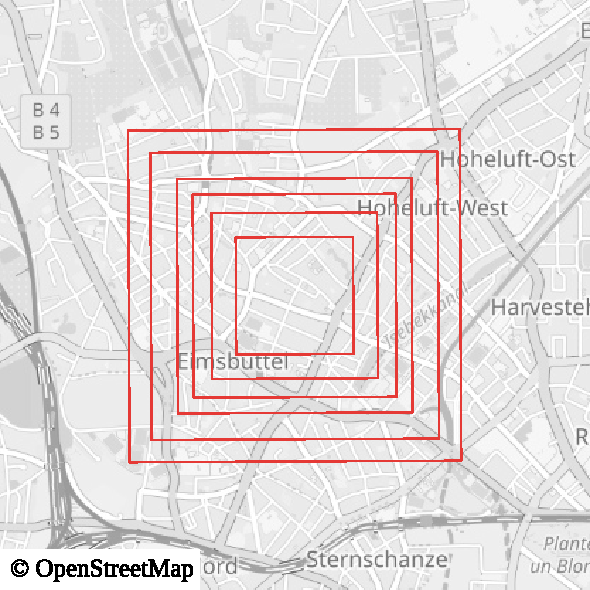
\includegraphics[width=\textwidth]{images/qgis-overview-city-rural_city}
					\end{figcenter}
				\end{minipage}
				\hspace{0.04\textwidth}
				\begin{minipage}[t]{.38\textwidth}
					\begin{figcenter}
						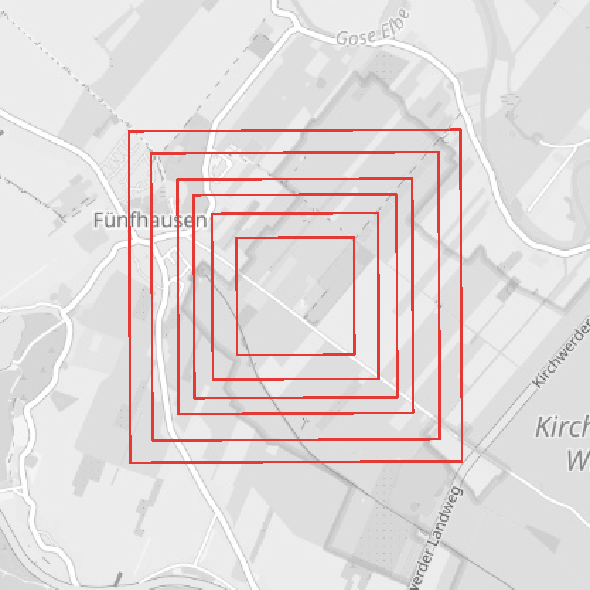
\includegraphics[width=\textwidth]{images/qgis-overview-city-rural_rural}
					\end{figcenter}
				\end{minipage}
				\caption[Areas of the \enquote{OSM city} and \enquote{OSM rural} datasets.]{All six regions from 0.5 km\textsuperscript{2} to 4 km\textsuperscript{2} of the \enquote{OSM city} datasets (left) and \enquote{OSM rural} datasets (right).}
			\end{figure}
		
		\subsubsection{Optimizations}
		
			As described in \Cref{chap:implementation}, several optimizations were made to the implementation.
			The effectiveness of these optimizations was evaluated using the 4 km\textsuperscript{2} \enquote{OSM city} dataset.
			Each of the following optimizations was deactivated or replaced for the evaluation:

			\begin{description}
				\item[Shadow areas] Instead, every visibility check was performed using the custom intersection check described in \Cref{subsubsec:intersection-checks}.
				\item[Custom intersection check] The custom intersection check was replaced by the \texttt{RobustLineIntersector} class from the NTS to determine intersections between line segments.
				\item[BinIndex] Instead, the \texttt{Bintree} from the NTS was used.
				\item[Convex hull] The restriction to only consider vertices on the convex hull of obstacles was removed.
				\item[Valid angle areas] Considering only potential visibility neighbors within certain angular ranges was deactivated.
				\item[kNN search] Instead, all visibility neighbors in all directions were determined.
			\end{description}		
			
		\subsubsection{Measurement method}
		
			Measuring the performance was done by a small agent-based simulation project called \texttt{HikerModel}, consisting of one agent consecutively visiting a given list of coordinates (routing waypoints) and using a given dataset as input to the hybrid routing algorithm.
			The coordinates are given via a linestring within a GeoJSON file, of which each coordinate of the linestring is visited by the agent in order.
			Each waypoint was within the range of the dataset, meaning each coordinate was surrounded by obstacles.
			The Euclidean distances (beeline distances) of the line segments within this linestring were distributed evenly to measure the required routing time relative to the distance and dataset size.
			
			Because the OSM datasets within one category cover differently sized areas, each waypoint linestring of an OSM-based dataset contains all waypoints of the next smaller one plus some additional ones.
			This means that the waypoints of the smallest dataset are also used by every other dataset.
		
		\subsubsection{Technical considerations}
		
			The measurement was done by an auxiliary class \texttt{PerformanceMeasurement}, which provides a method that measures the execution time of a passed function delegate.
			
			As part of its memory management, C\#/.NET uses automatic garbage collection, adding unavoidable noise to the measurements.
			Unfortunately, the garbage collector cannot be turned off and controlling it is only partially possible.
			
			Before each measurement, the garbage collector was triggered to provide equal circumstances to all iterations.
			This was done by the \texttt{GC.Collect()} and \texttt{GC.WaitForPendingFinalizers()} methods of the .NET framework.
			Using these two methods forces a garbage collection and waits for it to finish\footnote{\url{https://learn.microsoft.com/en-us/dotnet/api/system.gc.waitforpendingfinalizers?view=net-7.0}}.
			
			To prevent the garbage collection from interfering with the execution, a 256 MiB large no-GC-region is placed around the measured function call via \texttt{GC.TryStartNoGCRegion(256 * 1024 * 1024)}.
			Introducing this no-GC-region noticeably reduced noise in the measured times.
		
			C\#/.NET also uses \term*[just-in-time compilation]{just-in-time} (\term*{JIT}) compilation changing the code during runtime, which potentially yields different measurements for subsequent method calls.
			JIT compilation can not be turned off for regular .NET executions via the command \texttt{dotnet program.dll}.
			An alternative would be the usage of \term*[ahead-of-time compilation]{ahead-of-time} (\term*{AOT}) compilation, negatively affecting the performance of LINQ operations\footnote{\url{https://learn.microsoft.com/en-us/dotnet/core/deploying/native-aot/?tabs=net7}}, which are frequently used in the implementation.
			Because both compilation strategies have disadvantages, the default JIT compilation was chosen.
			
			The dynamic behavior of JIT compilation was mitigated by calling the measured function three times without storing the measurement results (warm-ups) before executing it five times and storing these last five results.
			This ensures that any JIT compilation and garbage collection of prior code was performed during the warm-up iterations and interfered with the actual iteration as little as possible.
			
			Another step to get stable and reproducible results was increasing the process priority to exclusively use one CPU core on which the single-threaded application ran.
			Increasing the process priority was done by settings the \texttt{Thread.CurrentThread.Priority} to \texttt{ProcessPriorityClass.High}, which required root permissions on Linux systems.
		
		\subsubsection{System and hardware}
		
			The measurements were performed on an up-to-date Arch Linux operating system (Kernel 6.4.3) with .NET Core 7.0.107 and MARS framework 4.5.2.
			Apart from necessary operating system processes and a minimal desktop environment, no other applications ran during the performance measurements.
			
			The hardware consisted of an octa-core Intel\textregistered\ Xeon\textregistered\ E3-1231 v3 CPU at 3.40 GHz, a total of 16GB DDR3 1333 MHz RAM and a Samsung EVO 850 SSD.
			However, the whole algorithm and the \texttt{HikerModel} simulation is single-threaded.
			File system operations are only performed to initially load the input data and to write the measurement results after completing all executions.
	
\section{Performance evaluation}

	In this section, the results of the performance evaluation of the hybrid routing algorithm are presented.
	First, results using OSM-based datasets are discussed, followed by the artificial pattern-based datasets.

	\subsection{OSM-based datasets}
		
		\subsubsection{Import and graph generation}
		
			A few aspects regarding the runtime behavior can be inferred from the general graph generation times shown in \Cref{fig:eval-import-city} and \Cref{fig:eval-import-rural}.
			First, as mentioned at the beginning of \Cref{subsec:related-work:visibility-graph}, the process of generating a visibility graph has an inherent quadratic runtime.
			This fact is directly visible in the import measurements shown in \Cref{fig:eval-import-city-abs} and \Cref{fig:eval-import-rural-abs}, even though it is less prominent in the \enquote{OSM rural} datasets.
%			Details on the contribution of each task to the overall graph generation time discussed below.
			Second, \Cref{fig:eval-import-city-rel} and \ref{fig:eval-import-rural-rel} show an increase in the per-vertex processing time, which not necessarily grows quadratic as the \enquote{OSM rural} dataset shows.
			
			\begin{figure}[h!]
				\begin{minipage}{.48\textwidth}
					\begin{subfigure}[t]{\linewidth}
						\begin{figcenter}
							\begingroup%
\makeatletter%
\begin{pgfpicture}%
\pgfpathrectangle{\pgfpointorigin}{\pgfqpoint{3.041406in}{1.869661in}}%
\pgfusepath{use as bounding box}%
\begin{pgfscope}%
\pgfsetbuttcap%
\pgfsetmiterjoin%
\definecolor{currentfill}{rgb}{1.000000,1.000000,1.000000}%
\pgfsetfillcolor{currentfill}%
\pgfsetlinewidth{0.000000pt}%
\definecolor{currentstroke}{rgb}{1.000000,1.000000,1.000000}%
\pgfsetstrokecolor{currentstroke}%
\pgfsetdash{}{0pt}%
\pgfpathmoveto{\pgfqpoint{0.000000in}{0.000000in}}%
\pgfpathlineto{\pgfqpoint{3.041406in}{0.000000in}}%
\pgfpathlineto{\pgfqpoint{3.041406in}{1.869661in}}%
\pgfpathlineto{\pgfqpoint{0.000000in}{1.869661in}}%
\pgfpathlineto{\pgfqpoint{0.000000in}{0.000000in}}%
\pgfpathclose%
\pgfusepath{fill}%
\end{pgfscope}%
\begin{pgfscope}%
\pgfsetbuttcap%
\pgfsetmiterjoin%
\definecolor{currentfill}{rgb}{1.000000,1.000000,1.000000}%
\pgfsetfillcolor{currentfill}%
\pgfsetlinewidth{0.000000pt}%
\definecolor{currentstroke}{rgb}{0.000000,0.000000,0.000000}%
\pgfsetstrokecolor{currentstroke}%
\pgfsetstrokeopacity{0.000000}%
\pgfsetdash{}{0pt}%
\pgfpathmoveto{\pgfqpoint{0.601779in}{0.451389in}}%
\pgfpathlineto{\pgfqpoint{3.041406in}{0.451389in}}%
\pgfpathlineto{\pgfqpoint{3.041406in}{1.848071in}}%
\pgfpathlineto{\pgfqpoint{0.601779in}{1.848071in}}%
\pgfpathlineto{\pgfqpoint{0.601779in}{0.451389in}}%
\pgfpathclose%
\pgfusepath{fill}%
\end{pgfscope}%
\begin{pgfscope}%
\pgfpathrectangle{\pgfqpoint{0.601779in}{0.451389in}}{\pgfqpoint{2.439626in}{1.396682in}}%
\pgfusepath{clip}%
\pgfsetroundcap%
\pgfsetroundjoin%
\pgfsetlinewidth{1.003750pt}%
\definecolor{currentstroke}{rgb}{0.800000,0.800000,0.800000}%
\pgfsetstrokecolor{currentstroke}%
\pgfsetdash{}{0pt}%
\pgfpathmoveto{\pgfqpoint{0.601779in}{0.451389in}}%
\pgfpathlineto{\pgfqpoint{0.601779in}{1.848071in}}%
\pgfusepath{stroke}%
\end{pgfscope}%
\begin{pgfscope}%
\definecolor{textcolor}{rgb}{0.150000,0.150000,0.150000}%
\pgfsetstrokecolor{textcolor}%
\pgfsetfillcolor{textcolor}%
\pgftext[x=0.601779in,y=0.319444in,,top]{\color{textcolor}\sffamily\fontsize{9.000000}{10.800000}\selectfont 0}%
\end{pgfscope}%
\begin{pgfscope}%
\pgfpathrectangle{\pgfqpoint{0.601779in}{0.451389in}}{\pgfqpoint{2.439626in}{1.396682in}}%
\pgfusepath{clip}%
\pgfsetroundcap%
\pgfsetroundjoin%
\pgfsetlinewidth{1.003750pt}%
\definecolor{currentstroke}{rgb}{0.800000,0.800000,0.800000}%
\pgfsetstrokecolor{currentstroke}%
\pgfsetdash{}{0pt}%
\pgfpathmoveto{\pgfqpoint{1.121799in}{0.451389in}}%
\pgfpathlineto{\pgfqpoint{1.121799in}{1.848071in}}%
\pgfusepath{stroke}%
\end{pgfscope}%
\begin{pgfscope}%
\definecolor{textcolor}{rgb}{0.150000,0.150000,0.150000}%
\pgfsetstrokecolor{textcolor}%
\pgfsetfillcolor{textcolor}%
\pgftext[x=1.121799in,y=0.319444in,,top]{\color{textcolor}\sffamily\fontsize{9.000000}{10.800000}\selectfont 10000}%
\end{pgfscope}%
\begin{pgfscope}%
\pgfpathrectangle{\pgfqpoint{0.601779in}{0.451389in}}{\pgfqpoint{2.439626in}{1.396682in}}%
\pgfusepath{clip}%
\pgfsetroundcap%
\pgfsetroundjoin%
\pgfsetlinewidth{1.003750pt}%
\definecolor{currentstroke}{rgb}{0.800000,0.800000,0.800000}%
\pgfsetstrokecolor{currentstroke}%
\pgfsetdash{}{0pt}%
\pgfpathmoveto{\pgfqpoint{1.641819in}{0.451389in}}%
\pgfpathlineto{\pgfqpoint{1.641819in}{1.848071in}}%
\pgfusepath{stroke}%
\end{pgfscope}%
\begin{pgfscope}%
\definecolor{textcolor}{rgb}{0.150000,0.150000,0.150000}%
\pgfsetstrokecolor{textcolor}%
\pgfsetfillcolor{textcolor}%
\pgftext[x=1.641819in,y=0.319444in,,top]{\color{textcolor}\sffamily\fontsize{9.000000}{10.800000}\selectfont 20000}%
\end{pgfscope}%
\begin{pgfscope}%
\pgfpathrectangle{\pgfqpoint{0.601779in}{0.451389in}}{\pgfqpoint{2.439626in}{1.396682in}}%
\pgfusepath{clip}%
\pgfsetroundcap%
\pgfsetroundjoin%
\pgfsetlinewidth{1.003750pt}%
\definecolor{currentstroke}{rgb}{0.800000,0.800000,0.800000}%
\pgfsetstrokecolor{currentstroke}%
\pgfsetdash{}{0pt}%
\pgfpathmoveto{\pgfqpoint{2.161839in}{0.451389in}}%
\pgfpathlineto{\pgfqpoint{2.161839in}{1.848071in}}%
\pgfusepath{stroke}%
\end{pgfscope}%
\begin{pgfscope}%
\definecolor{textcolor}{rgb}{0.150000,0.150000,0.150000}%
\pgfsetstrokecolor{textcolor}%
\pgfsetfillcolor{textcolor}%
\pgftext[x=2.161839in,y=0.319444in,,top]{\color{textcolor}\sffamily\fontsize{9.000000}{10.800000}\selectfont 30000}%
\end{pgfscope}%
\begin{pgfscope}%
\pgfpathrectangle{\pgfqpoint{0.601779in}{0.451389in}}{\pgfqpoint{2.439626in}{1.396682in}}%
\pgfusepath{clip}%
\pgfsetroundcap%
\pgfsetroundjoin%
\pgfsetlinewidth{1.003750pt}%
\definecolor{currentstroke}{rgb}{0.800000,0.800000,0.800000}%
\pgfsetstrokecolor{currentstroke}%
\pgfsetdash{}{0pt}%
\pgfpathmoveto{\pgfqpoint{2.681859in}{0.451389in}}%
\pgfpathlineto{\pgfqpoint{2.681859in}{1.848071in}}%
\pgfusepath{stroke}%
\end{pgfscope}%
\begin{pgfscope}%
\definecolor{textcolor}{rgb}{0.150000,0.150000,0.150000}%
\pgfsetstrokecolor{textcolor}%
\pgfsetfillcolor{textcolor}%
\pgftext[x=2.681859in,y=0.319444in,,top]{\color{textcolor}\sffamily\fontsize{9.000000}{10.800000}\selectfont 40000}%
\end{pgfscope}%
\begin{pgfscope}%
\definecolor{textcolor}{rgb}{0.150000,0.150000,0.150000}%
\pgfsetstrokecolor{textcolor}%
\pgfsetfillcolor{textcolor}%
\pgftext[x=1.821593in,y=0.125000in,,top]{\color{textcolor}\sffamily\fontsize{9.000000}{10.800000}\selectfont Input obstacle vertices}%
\end{pgfscope}%
\begin{pgfscope}%
\pgfpathrectangle{\pgfqpoint{0.601779in}{0.451389in}}{\pgfqpoint{2.439626in}{1.396682in}}%
\pgfusepath{clip}%
\pgfsetroundcap%
\pgfsetroundjoin%
\pgfsetlinewidth{1.003750pt}%
\definecolor{currentstroke}{rgb}{0.800000,0.800000,0.800000}%
\pgfsetstrokecolor{currentstroke}%
\pgfsetdash{}{0pt}%
\pgfpathmoveto{\pgfqpoint{0.601779in}{0.451389in}}%
\pgfpathlineto{\pgfqpoint{3.041406in}{0.451389in}}%
\pgfusepath{stroke}%
\end{pgfscope}%
\begin{pgfscope}%
\definecolor{textcolor}{rgb}{0.150000,0.150000,0.150000}%
\pgfsetstrokecolor{textcolor}%
\pgfsetfillcolor{textcolor}%
\pgftext[x=0.400987in, y=0.403903in, left, base]{\color{textcolor}\sffamily\fontsize{9.000000}{10.800000}\selectfont 0}%
\end{pgfscope}%
\begin{pgfscope}%
\pgfpathrectangle{\pgfqpoint{0.601779in}{0.451389in}}{\pgfqpoint{2.439626in}{1.396682in}}%
\pgfusepath{clip}%
\pgfsetroundcap%
\pgfsetroundjoin%
\pgfsetlinewidth{1.003750pt}%
\definecolor{currentstroke}{rgb}{0.800000,0.800000,0.800000}%
\pgfsetstrokecolor{currentstroke}%
\pgfsetdash{}{0pt}%
\pgfpathmoveto{\pgfqpoint{0.601779in}{0.794085in}}%
\pgfpathlineto{\pgfqpoint{3.041406in}{0.794085in}}%
\pgfusepath{stroke}%
\end{pgfscope}%
\begin{pgfscope}%
\definecolor{textcolor}{rgb}{0.150000,0.150000,0.150000}%
\pgfsetstrokecolor{textcolor}%
\pgfsetfillcolor{textcolor}%
\pgftext[x=0.263292in, y=0.746600in, left, base]{\color{textcolor}\sffamily\fontsize{9.000000}{10.800000}\selectfont 250}%
\end{pgfscope}%
\begin{pgfscope}%
\pgfpathrectangle{\pgfqpoint{0.601779in}{0.451389in}}{\pgfqpoint{2.439626in}{1.396682in}}%
\pgfusepath{clip}%
\pgfsetroundcap%
\pgfsetroundjoin%
\pgfsetlinewidth{1.003750pt}%
\definecolor{currentstroke}{rgb}{0.800000,0.800000,0.800000}%
\pgfsetstrokecolor{currentstroke}%
\pgfsetdash{}{0pt}%
\pgfpathmoveto{\pgfqpoint{0.601779in}{1.136782in}}%
\pgfpathlineto{\pgfqpoint{3.041406in}{1.136782in}}%
\pgfusepath{stroke}%
\end{pgfscope}%
\begin{pgfscope}%
\definecolor{textcolor}{rgb}{0.150000,0.150000,0.150000}%
\pgfsetstrokecolor{textcolor}%
\pgfsetfillcolor{textcolor}%
\pgftext[x=0.263292in, y=1.089297in, left, base]{\color{textcolor}\sffamily\fontsize{9.000000}{10.800000}\selectfont 500}%
\end{pgfscope}%
\begin{pgfscope}%
\pgfpathrectangle{\pgfqpoint{0.601779in}{0.451389in}}{\pgfqpoint{2.439626in}{1.396682in}}%
\pgfusepath{clip}%
\pgfsetroundcap%
\pgfsetroundjoin%
\pgfsetlinewidth{1.003750pt}%
\definecolor{currentstroke}{rgb}{0.800000,0.800000,0.800000}%
\pgfsetstrokecolor{currentstroke}%
\pgfsetdash{}{0pt}%
\pgfpathmoveto{\pgfqpoint{0.601779in}{1.479479in}}%
\pgfpathlineto{\pgfqpoint{3.041406in}{1.479479in}}%
\pgfusepath{stroke}%
\end{pgfscope}%
\begin{pgfscope}%
\definecolor{textcolor}{rgb}{0.150000,0.150000,0.150000}%
\pgfsetstrokecolor{textcolor}%
\pgfsetfillcolor{textcolor}%
\pgftext[x=0.263292in, y=1.431993in, left, base]{\color{textcolor}\sffamily\fontsize{9.000000}{10.800000}\selectfont 750}%
\end{pgfscope}%
\begin{pgfscope}%
\pgfpathrectangle{\pgfqpoint{0.601779in}{0.451389in}}{\pgfqpoint{2.439626in}{1.396682in}}%
\pgfusepath{clip}%
\pgfsetroundcap%
\pgfsetroundjoin%
\pgfsetlinewidth{1.003750pt}%
\definecolor{currentstroke}{rgb}{0.800000,0.800000,0.800000}%
\pgfsetstrokecolor{currentstroke}%
\pgfsetdash{}{0pt}%
\pgfpathmoveto{\pgfqpoint{0.601779in}{1.822175in}}%
\pgfpathlineto{\pgfqpoint{3.041406in}{1.822175in}}%
\pgfusepath{stroke}%
\end{pgfscope}%
\begin{pgfscope}%
\definecolor{textcolor}{rgb}{0.150000,0.150000,0.150000}%
\pgfsetstrokecolor{textcolor}%
\pgfsetfillcolor{textcolor}%
\pgftext[x=0.194444in, y=1.774690in, left, base]{\color{textcolor}\sffamily\fontsize{9.000000}{10.800000}\selectfont 1000}%
\end{pgfscope}%
\begin{pgfscope}%
\definecolor{textcolor}{rgb}{0.150000,0.150000,0.150000}%
\pgfsetstrokecolor{textcolor}%
\pgfsetfillcolor{textcolor}%
\pgftext[x=0.125000in,y=1.149730in,,bottom,rotate=90.000000]{\color{textcolor}\sffamily\fontsize{9.000000}{10.800000}\selectfont Time in s}%
\end{pgfscope}%
\begin{pgfscope}%
\pgfpathrectangle{\pgfqpoint{0.601779in}{0.451389in}}{\pgfqpoint{2.439626in}{1.396682in}}%
\pgfusepath{clip}%
\pgfsetbuttcap%
\pgfsetroundjoin%
\definecolor{currentfill}{rgb}{0.003922,0.450980,0.698039}%
\pgfsetfillcolor{currentfill}%
\pgfsetfillopacity{0.200000}%
\pgfsetlinewidth{1.003750pt}%
\definecolor{currentstroke}{rgb}{0.003922,0.450980,0.698039}%
\pgfsetstrokecolor{currentstroke}%
\pgfsetstrokeopacity{0.200000}%
\pgfsetdash{}{0pt}%
\pgfsys@defobject{currentmarker}{\pgfqpoint{0.970786in}{0.475103in}}{\pgfqpoint{2.942805in}{1.782692in}}{%
\pgfpathmoveto{\pgfqpoint{0.970786in}{0.475365in}}%
\pgfpathlineto{\pgfqpoint{0.970786in}{0.475103in}}%
\pgfpathlineto{\pgfqpoint{1.270421in}{0.525314in}}%
\pgfpathlineto{\pgfqpoint{1.532303in}{0.609750in}}%
\pgfpathlineto{\pgfqpoint{1.787477in}{0.734608in}}%
\pgfpathlineto{\pgfqpoint{2.380975in}{1.150136in}}%
\pgfpathlineto{\pgfqpoint{2.942805in}{1.763790in}}%
\pgfpathlineto{\pgfqpoint{2.942805in}{1.782692in}}%
\pgfpathlineto{\pgfqpoint{2.942805in}{1.782692in}}%
\pgfpathlineto{\pgfqpoint{2.380975in}{1.159429in}}%
\pgfpathlineto{\pgfqpoint{1.787477in}{0.735896in}}%
\pgfpathlineto{\pgfqpoint{1.532303in}{0.612478in}}%
\pgfpathlineto{\pgfqpoint{1.270421in}{0.526536in}}%
\pgfpathlineto{\pgfqpoint{0.970786in}{0.475365in}}%
\pgfpathlineto{\pgfqpoint{0.970786in}{0.475365in}}%
\pgfpathclose%
\pgfusepath{stroke,fill}%
}%
\begin{pgfscope}%
\pgfsys@transformshift{0.000000in}{0.000000in}%
\pgfsys@useobject{currentmarker}{}%
\end{pgfscope}%
\end{pgfscope}%
\begin{pgfscope}%
\pgfsetrectcap%
\pgfsetmiterjoin%
\pgfsetlinewidth{1.254687pt}%
\definecolor{currentstroke}{rgb}{0.800000,0.800000,0.800000}%
\pgfsetstrokecolor{currentstroke}%
\pgfsetdash{}{0pt}%
\pgfpathmoveto{\pgfqpoint{0.601779in}{0.451389in}}%
\pgfpathlineto{\pgfqpoint{0.601779in}{1.848071in}}%
\pgfusepath{stroke}%
\end{pgfscope}%
\begin{pgfscope}%
\pgfsetrectcap%
\pgfsetmiterjoin%
\pgfsetlinewidth{1.254687pt}%
\definecolor{currentstroke}{rgb}{0.800000,0.800000,0.800000}%
\pgfsetstrokecolor{currentstroke}%
\pgfsetdash{}{0pt}%
\pgfpathmoveto{\pgfqpoint{3.041406in}{0.451389in}}%
\pgfpathlineto{\pgfqpoint{3.041406in}{1.848071in}}%
\pgfusepath{stroke}%
\end{pgfscope}%
\begin{pgfscope}%
\pgfsetrectcap%
\pgfsetmiterjoin%
\pgfsetlinewidth{1.254687pt}%
\definecolor{currentstroke}{rgb}{0.800000,0.800000,0.800000}%
\pgfsetstrokecolor{currentstroke}%
\pgfsetdash{}{0pt}%
\pgfpathmoveto{\pgfqpoint{0.601779in}{0.451389in}}%
\pgfpathlineto{\pgfqpoint{3.041406in}{0.451389in}}%
\pgfusepath{stroke}%
\end{pgfscope}%
\begin{pgfscope}%
\pgfsetrectcap%
\pgfsetmiterjoin%
\pgfsetlinewidth{1.254687pt}%
\definecolor{currentstroke}{rgb}{0.800000,0.800000,0.800000}%
\pgfsetstrokecolor{currentstroke}%
\pgfsetdash{}{0pt}%
\pgfpathmoveto{\pgfqpoint{0.601779in}{1.848071in}}%
\pgfpathlineto{\pgfqpoint{3.041406in}{1.848071in}}%
\pgfusepath{stroke}%
\end{pgfscope}%
\begin{pgfscope}%
\pgfsetroundcap%
\pgfsetroundjoin%
\pgfsetlinewidth{1.003750pt}%
\definecolor{currentstroke}{rgb}{0.003922,0.450980,0.698039}%
\pgfsetstrokecolor{currentstroke}%
\pgfsetdash{}{0pt}%
\pgfpathmoveto{\pgfqpoint{0.970786in}{0.475218in}}%
\pgfpathlineto{\pgfqpoint{1.270421in}{0.525877in}}%
\pgfpathlineto{\pgfqpoint{1.532303in}{0.611282in}}%
\pgfpathlineto{\pgfqpoint{1.787477in}{0.735321in}}%
\pgfpathlineto{\pgfqpoint{2.380975in}{1.154498in}}%
\pgfpathlineto{\pgfqpoint{2.942805in}{1.771598in}}%
\pgfusepath{stroke}%
\end{pgfscope}%
\begin{pgfscope}%
\pgfsetbuttcap%
\pgfsetroundjoin%
\definecolor{currentfill}{rgb}{0.003922,0.450980,0.698039}%
\pgfsetfillcolor{currentfill}%
\pgfsetlinewidth{0.752812pt}%
\definecolor{currentstroke}{rgb}{1.000000,1.000000,1.000000}%
\pgfsetstrokecolor{currentstroke}%
\pgfsetdash{}{0pt}%
\pgfsys@defobject{currentmarker}{\pgfqpoint{-0.034722in}{-0.034722in}}{\pgfqpoint{0.034722in}{0.034722in}}{%
\pgfpathmoveto{\pgfqpoint{0.000000in}{-0.034722in}}%
\pgfpathcurveto{\pgfqpoint{0.009208in}{-0.034722in}}{\pgfqpoint{0.018041in}{-0.031064in}}{\pgfqpoint{0.024552in}{-0.024552in}}%
\pgfpathcurveto{\pgfqpoint{0.031064in}{-0.018041in}}{\pgfqpoint{0.034722in}{-0.009208in}}{\pgfqpoint{0.034722in}{0.000000in}}%
\pgfpathcurveto{\pgfqpoint{0.034722in}{0.009208in}}{\pgfqpoint{0.031064in}{0.018041in}}{\pgfqpoint{0.024552in}{0.024552in}}%
\pgfpathcurveto{\pgfqpoint{0.018041in}{0.031064in}}{\pgfqpoint{0.009208in}{0.034722in}}{\pgfqpoint{0.000000in}{0.034722in}}%
\pgfpathcurveto{\pgfqpoint{-0.009208in}{0.034722in}}{\pgfqpoint{-0.018041in}{0.031064in}}{\pgfqpoint{-0.024552in}{0.024552in}}%
\pgfpathcurveto{\pgfqpoint{-0.031064in}{0.018041in}}{\pgfqpoint{-0.034722in}{0.009208in}}{\pgfqpoint{-0.034722in}{0.000000in}}%
\pgfpathcurveto{\pgfqpoint{-0.034722in}{-0.009208in}}{\pgfqpoint{-0.031064in}{-0.018041in}}{\pgfqpoint{-0.024552in}{-0.024552in}}%
\pgfpathcurveto{\pgfqpoint{-0.018041in}{-0.031064in}}{\pgfqpoint{-0.009208in}{-0.034722in}}{\pgfqpoint{0.000000in}{-0.034722in}}%
\pgfpathlineto{\pgfqpoint{0.000000in}{-0.034722in}}%
\pgfpathclose%
\pgfusepath{stroke,fill}%
}%
\begin{pgfscope}%
\pgfsys@transformshift{0.970786in}{0.475218in}%
\pgfsys@useobject{currentmarker}{}%
\end{pgfscope}%
\begin{pgfscope}%
\pgfsys@transformshift{1.270421in}{0.525877in}%
\pgfsys@useobject{currentmarker}{}%
\end{pgfscope}%
\begin{pgfscope}%
\pgfsys@transformshift{1.532303in}{0.611282in}%
\pgfsys@useobject{currentmarker}{}%
\end{pgfscope}%
\begin{pgfscope}%
\pgfsys@transformshift{1.787477in}{0.735321in}%
\pgfsys@useobject{currentmarker}{}%
\end{pgfscope}%
\begin{pgfscope}%
\pgfsys@transformshift{2.380975in}{1.154498in}%
\pgfsys@useobject{currentmarker}{}%
\end{pgfscope}%
\begin{pgfscope}%
\pgfsys@transformshift{2.942805in}{1.771598in}%
\pgfsys@useobject{currentmarker}{}%
\end{pgfscope}%
\end{pgfscope}%
\end{pgfpicture}%
\makeatother%
\endgroup%

						\end{figcenter}
						\caption{Total graph generation times.}
						\label{fig:eval-import-city-abs}
					\end{subfigure}
					\\[3ex]
					\begin{subfigure}[t]{\linewidth}
						\begin{figcenter}
							\begingroup%
\makeatletter%
\begin{pgfpicture}%
\pgfpathrectangle{\pgfpointorigin}{\pgfqpoint{3.043196in}{1.867995in}}%
\pgfusepath{use as bounding box}%
\begin{pgfscope}%
\pgfsetbuttcap%
\pgfsetmiterjoin%
\definecolor{currentfill}{rgb}{1.000000,1.000000,1.000000}%
\pgfsetfillcolor{currentfill}%
\pgfsetlinewidth{0.000000pt}%
\definecolor{currentstroke}{rgb}{1.000000,1.000000,1.000000}%
\pgfsetstrokecolor{currentstroke}%
\pgfsetdash{}{0pt}%
\pgfpathmoveto{\pgfqpoint{0.000000in}{0.000000in}}%
\pgfpathlineto{\pgfqpoint{3.043196in}{0.000000in}}%
\pgfpathlineto{\pgfqpoint{3.043196in}{1.867995in}}%
\pgfpathlineto{\pgfqpoint{0.000000in}{1.867995in}}%
\pgfpathlineto{\pgfqpoint{0.000000in}{0.000000in}}%
\pgfpathclose%
\pgfusepath{fill}%
\end{pgfscope}%
\begin{pgfscope}%
\pgfsetbuttcap%
\pgfsetmiterjoin%
\definecolor{currentfill}{rgb}{1.000000,1.000000,1.000000}%
\pgfsetfillcolor{currentfill}%
\pgfsetlinewidth{0.000000pt}%
\definecolor{currentstroke}{rgb}{0.000000,0.000000,0.000000}%
\pgfsetstrokecolor{currentstroke}%
\pgfsetstrokeopacity{0.000000}%
\pgfsetdash{}{0pt}%
\pgfpathmoveto{\pgfqpoint{0.395236in}{0.451389in}}%
\pgfpathlineto{\pgfqpoint{3.043196in}{0.451389in}}%
\pgfpathlineto{\pgfqpoint{3.043196in}{1.867995in}}%
\pgfpathlineto{\pgfqpoint{0.395236in}{1.867995in}}%
\pgfpathlineto{\pgfqpoint{0.395236in}{0.451389in}}%
\pgfpathclose%
\pgfusepath{fill}%
\end{pgfscope}%
\begin{pgfscope}%
\pgfpathrectangle{\pgfqpoint{0.395236in}{0.451389in}}{\pgfqpoint{2.647959in}{1.416606in}}%
\pgfusepath{clip}%
\pgfsetroundcap%
\pgfsetroundjoin%
\pgfsetlinewidth{1.003750pt}%
\definecolor{currentstroke}{rgb}{0.800000,0.800000,0.800000}%
\pgfsetstrokecolor{currentstroke}%
\pgfsetdash{}{0pt}%
\pgfpathmoveto{\pgfqpoint{0.395236in}{0.451389in}}%
\pgfpathlineto{\pgfqpoint{0.395236in}{1.867995in}}%
\pgfusepath{stroke}%
\end{pgfscope}%
\begin{pgfscope}%
\definecolor{textcolor}{rgb}{0.150000,0.150000,0.150000}%
\pgfsetstrokecolor{textcolor}%
\pgfsetfillcolor{textcolor}%
\pgftext[x=0.395236in,y=0.319444in,,top]{\color{textcolor}\sffamily\fontsize{9.000000}{10.800000}\selectfont 0}%
\end{pgfscope}%
\begin{pgfscope}%
\pgfpathrectangle{\pgfqpoint{0.395236in}{0.451389in}}{\pgfqpoint{2.647959in}{1.416606in}}%
\pgfusepath{clip}%
\pgfsetroundcap%
\pgfsetroundjoin%
\pgfsetlinewidth{1.003750pt}%
\definecolor{currentstroke}{rgb}{0.800000,0.800000,0.800000}%
\pgfsetstrokecolor{currentstroke}%
\pgfsetdash{}{0pt}%
\pgfpathmoveto{\pgfqpoint{0.800662in}{0.451389in}}%
\pgfpathlineto{\pgfqpoint{0.800662in}{1.867995in}}%
\pgfusepath{stroke}%
\end{pgfscope}%
\begin{pgfscope}%
\definecolor{textcolor}{rgb}{0.150000,0.150000,0.150000}%
\pgfsetstrokecolor{textcolor}%
\pgfsetfillcolor{textcolor}%
\pgftext[x=0.800662in,y=0.319444in,,top]{\color{textcolor}\sffamily\fontsize{9.000000}{10.800000}\selectfont 5000}%
\end{pgfscope}%
\begin{pgfscope}%
\pgfpathrectangle{\pgfqpoint{0.395236in}{0.451389in}}{\pgfqpoint{2.647959in}{1.416606in}}%
\pgfusepath{clip}%
\pgfsetroundcap%
\pgfsetroundjoin%
\pgfsetlinewidth{1.003750pt}%
\definecolor{currentstroke}{rgb}{0.800000,0.800000,0.800000}%
\pgfsetstrokecolor{currentstroke}%
\pgfsetdash{}{0pt}%
\pgfpathmoveto{\pgfqpoint{1.206089in}{0.451389in}}%
\pgfpathlineto{\pgfqpoint{1.206089in}{1.867995in}}%
\pgfusepath{stroke}%
\end{pgfscope}%
\begin{pgfscope}%
\definecolor{textcolor}{rgb}{0.150000,0.150000,0.150000}%
\pgfsetstrokecolor{textcolor}%
\pgfsetfillcolor{textcolor}%
\pgftext[x=1.206089in,y=0.319444in,,top]{\color{textcolor}\sffamily\fontsize{9.000000}{10.800000}\selectfont 10000}%
\end{pgfscope}%
\begin{pgfscope}%
\pgfpathrectangle{\pgfqpoint{0.395236in}{0.451389in}}{\pgfqpoint{2.647959in}{1.416606in}}%
\pgfusepath{clip}%
\pgfsetroundcap%
\pgfsetroundjoin%
\pgfsetlinewidth{1.003750pt}%
\definecolor{currentstroke}{rgb}{0.800000,0.800000,0.800000}%
\pgfsetstrokecolor{currentstroke}%
\pgfsetdash{}{0pt}%
\pgfpathmoveto{\pgfqpoint{1.611515in}{0.451389in}}%
\pgfpathlineto{\pgfqpoint{1.611515in}{1.867995in}}%
\pgfusepath{stroke}%
\end{pgfscope}%
\begin{pgfscope}%
\definecolor{textcolor}{rgb}{0.150000,0.150000,0.150000}%
\pgfsetstrokecolor{textcolor}%
\pgfsetfillcolor{textcolor}%
\pgftext[x=1.611515in,y=0.319444in,,top]{\color{textcolor}\sffamily\fontsize{9.000000}{10.800000}\selectfont 15000}%
\end{pgfscope}%
\begin{pgfscope}%
\pgfpathrectangle{\pgfqpoint{0.395236in}{0.451389in}}{\pgfqpoint{2.647959in}{1.416606in}}%
\pgfusepath{clip}%
\pgfsetroundcap%
\pgfsetroundjoin%
\pgfsetlinewidth{1.003750pt}%
\definecolor{currentstroke}{rgb}{0.800000,0.800000,0.800000}%
\pgfsetstrokecolor{currentstroke}%
\pgfsetdash{}{0pt}%
\pgfpathmoveto{\pgfqpoint{2.016941in}{0.451389in}}%
\pgfpathlineto{\pgfqpoint{2.016941in}{1.867995in}}%
\pgfusepath{stroke}%
\end{pgfscope}%
\begin{pgfscope}%
\definecolor{textcolor}{rgb}{0.150000,0.150000,0.150000}%
\pgfsetstrokecolor{textcolor}%
\pgfsetfillcolor{textcolor}%
\pgftext[x=2.016941in,y=0.319444in,,top]{\color{textcolor}\sffamily\fontsize{9.000000}{10.800000}\selectfont 20000}%
\end{pgfscope}%
\begin{pgfscope}%
\pgfpathrectangle{\pgfqpoint{0.395236in}{0.451389in}}{\pgfqpoint{2.647959in}{1.416606in}}%
\pgfusepath{clip}%
\pgfsetroundcap%
\pgfsetroundjoin%
\pgfsetlinewidth{1.003750pt}%
\definecolor{currentstroke}{rgb}{0.800000,0.800000,0.800000}%
\pgfsetstrokecolor{currentstroke}%
\pgfsetdash{}{0pt}%
\pgfpathmoveto{\pgfqpoint{2.422367in}{0.451389in}}%
\pgfpathlineto{\pgfqpoint{2.422367in}{1.867995in}}%
\pgfusepath{stroke}%
\end{pgfscope}%
\begin{pgfscope}%
\definecolor{textcolor}{rgb}{0.150000,0.150000,0.150000}%
\pgfsetstrokecolor{textcolor}%
\pgfsetfillcolor{textcolor}%
\pgftext[x=2.422367in,y=0.319444in,,top]{\color{textcolor}\sffamily\fontsize{9.000000}{10.800000}\selectfont 25000}%
\end{pgfscope}%
\begin{pgfscope}%
\pgfpathrectangle{\pgfqpoint{0.395236in}{0.451389in}}{\pgfqpoint{2.647959in}{1.416606in}}%
\pgfusepath{clip}%
\pgfsetroundcap%
\pgfsetroundjoin%
\pgfsetlinewidth{1.003750pt}%
\definecolor{currentstroke}{rgb}{0.800000,0.800000,0.800000}%
\pgfsetstrokecolor{currentstroke}%
\pgfsetdash{}{0pt}%
\pgfpathmoveto{\pgfqpoint{2.827793in}{0.451389in}}%
\pgfpathlineto{\pgfqpoint{2.827793in}{1.867995in}}%
\pgfusepath{stroke}%
\end{pgfscope}%
\begin{pgfscope}%
\definecolor{textcolor}{rgb}{0.150000,0.150000,0.150000}%
\pgfsetstrokecolor{textcolor}%
\pgfsetfillcolor{textcolor}%
\pgftext[x=2.827793in,y=0.319444in,,top]{\color{textcolor}\sffamily\fontsize{9.000000}{10.800000}\selectfont 30000}%
\end{pgfscope}%
\begin{pgfscope}%
\definecolor{textcolor}{rgb}{0.150000,0.150000,0.150000}%
\pgfsetstrokecolor{textcolor}%
\pgfsetfillcolor{textcolor}%
\pgftext[x=1.719216in,y=0.125000in,,top]{\color{textcolor}\sffamily\fontsize{9.000000}{10.800000}\selectfont Input obstacle vertices}%
\end{pgfscope}%
\begin{pgfscope}%
\pgfpathrectangle{\pgfqpoint{0.395236in}{0.451389in}}{\pgfqpoint{2.647959in}{1.416606in}}%
\pgfusepath{clip}%
\pgfsetroundcap%
\pgfsetroundjoin%
\pgfsetlinewidth{1.003750pt}%
\definecolor{currentstroke}{rgb}{0.800000,0.800000,0.800000}%
\pgfsetstrokecolor{currentstroke}%
\pgfsetdash{}{0pt}%
\pgfpathmoveto{\pgfqpoint{0.395236in}{0.451389in}}%
\pgfpathlineto{\pgfqpoint{3.043196in}{0.451389in}}%
\pgfusepath{stroke}%
\end{pgfscope}%
\begin{pgfscope}%
\definecolor{textcolor}{rgb}{0.150000,0.150000,0.150000}%
\pgfsetstrokecolor{textcolor}%
\pgfsetfillcolor{textcolor}%
\pgftext[x=0.194444in, y=0.403903in, left, base]{\color{textcolor}\sffamily\fontsize{9.000000}{10.800000}\selectfont 0}%
\end{pgfscope}%
\begin{pgfscope}%
\pgfpathrectangle{\pgfqpoint{0.395236in}{0.451389in}}{\pgfqpoint{2.647959in}{1.416606in}}%
\pgfusepath{clip}%
\pgfsetroundcap%
\pgfsetroundjoin%
\pgfsetlinewidth{1.003750pt}%
\definecolor{currentstroke}{rgb}{0.800000,0.800000,0.800000}%
\pgfsetstrokecolor{currentstroke}%
\pgfsetdash{}{0pt}%
\pgfpathmoveto{\pgfqpoint{0.395236in}{0.854358in}}%
\pgfpathlineto{\pgfqpoint{3.043196in}{0.854358in}}%
\pgfusepath{stroke}%
\end{pgfscope}%
\begin{pgfscope}%
\definecolor{textcolor}{rgb}{0.150000,0.150000,0.150000}%
\pgfsetstrokecolor{textcolor}%
\pgfsetfillcolor{textcolor}%
\pgftext[x=0.194444in, y=0.806873in, left, base]{\color{textcolor}\sffamily\fontsize{9.000000}{10.800000}\selectfont 2}%
\end{pgfscope}%
\begin{pgfscope}%
\pgfpathrectangle{\pgfqpoint{0.395236in}{0.451389in}}{\pgfqpoint{2.647959in}{1.416606in}}%
\pgfusepath{clip}%
\pgfsetroundcap%
\pgfsetroundjoin%
\pgfsetlinewidth{1.003750pt}%
\definecolor{currentstroke}{rgb}{0.800000,0.800000,0.800000}%
\pgfsetstrokecolor{currentstroke}%
\pgfsetdash{}{0pt}%
\pgfpathmoveto{\pgfqpoint{0.395236in}{1.257328in}}%
\pgfpathlineto{\pgfqpoint{3.043196in}{1.257328in}}%
\pgfusepath{stroke}%
\end{pgfscope}%
\begin{pgfscope}%
\definecolor{textcolor}{rgb}{0.150000,0.150000,0.150000}%
\pgfsetstrokecolor{textcolor}%
\pgfsetfillcolor{textcolor}%
\pgftext[x=0.194444in, y=1.209842in, left, base]{\color{textcolor}\sffamily\fontsize{9.000000}{10.800000}\selectfont 4}%
\end{pgfscope}%
\begin{pgfscope}%
\pgfpathrectangle{\pgfqpoint{0.395236in}{0.451389in}}{\pgfqpoint{2.647959in}{1.416606in}}%
\pgfusepath{clip}%
\pgfsetroundcap%
\pgfsetroundjoin%
\pgfsetlinewidth{1.003750pt}%
\definecolor{currentstroke}{rgb}{0.800000,0.800000,0.800000}%
\pgfsetstrokecolor{currentstroke}%
\pgfsetdash{}{0pt}%
\pgfpathmoveto{\pgfqpoint{0.395236in}{1.660297in}}%
\pgfpathlineto{\pgfqpoint{3.043196in}{1.660297in}}%
\pgfusepath{stroke}%
\end{pgfscope}%
\begin{pgfscope}%
\definecolor{textcolor}{rgb}{0.150000,0.150000,0.150000}%
\pgfsetstrokecolor{textcolor}%
\pgfsetfillcolor{textcolor}%
\pgftext[x=0.194444in, y=1.612812in, left, base]{\color{textcolor}\sffamily\fontsize{9.000000}{10.800000}\selectfont 6}%
\end{pgfscope}%
\begin{pgfscope}%
\definecolor{textcolor}{rgb}{0.150000,0.150000,0.150000}%
\pgfsetstrokecolor{textcolor}%
\pgfsetfillcolor{textcolor}%
\pgftext[x=0.125000in,y=1.159692in,,bottom,rotate=90.000000]{\color{textcolor}\sffamily\fontsize{9.000000}{10.800000}\selectfont Time in ms}%
\end{pgfscope}%
\begin{pgfscope}%
\pgfpathrectangle{\pgfqpoint{0.395236in}{0.451389in}}{\pgfqpoint{2.647959in}{1.416606in}}%
\pgfusepath{clip}%
\pgfsetbuttcap%
\pgfsetroundjoin%
\definecolor{currentfill}{rgb}{0.003922,0.450980,0.698039}%
\pgfsetfillcolor{currentfill}%
\pgfsetfillopacity{0.200000}%
\pgfsetlinewidth{1.003750pt}%
\definecolor{currentstroke}{rgb}{0.003922,0.450980,0.698039}%
\pgfsetstrokecolor{currentstroke}%
\pgfsetstrokeopacity{0.200000}%
\pgfsetdash{}{0pt}%
\pgfsys@defobject{currentmarker}{\pgfqpoint{0.399615in}{0.472653in}}{\pgfqpoint{2.917311in}{1.801550in}}{%
\pgfpathmoveto{\pgfqpoint{0.399615in}{0.483482in}}%
\pgfpathlineto{\pgfqpoint{0.399615in}{0.472653in}}%
\pgfpathlineto{\pgfqpoint{0.412751in}{0.490586in}}%
\pgfpathlineto{\pgfqpoint{0.465294in}{0.494104in}}%
\pgfpathlineto{\pgfqpoint{0.552866in}{0.542933in}}%
\pgfpathlineto{\pgfqpoint{0.675467in}{0.592283in}}%
\pgfpathlineto{\pgfqpoint{0.833097in}{0.656559in}}%
\pgfpathlineto{\pgfqpoint{1.025755in}{0.752049in}}%
\pgfpathlineto{\pgfqpoint{1.253442in}{0.853539in}}%
\pgfpathlineto{\pgfqpoint{1.516158in}{0.976622in}}%
\pgfpathlineto{\pgfqpoint{1.813903in}{1.168476in}}%
\pgfpathlineto{\pgfqpoint{2.146677in}{1.309545in}}%
\pgfpathlineto{\pgfqpoint{2.514480in}{1.529714in}}%
\pgfpathlineto{\pgfqpoint{2.917311in}{1.794932in}}%
\pgfpathlineto{\pgfqpoint{2.917311in}{1.801550in}}%
\pgfpathlineto{\pgfqpoint{2.917311in}{1.801550in}}%
\pgfpathlineto{\pgfqpoint{2.514480in}{1.535942in}}%
\pgfpathlineto{\pgfqpoint{2.146677in}{1.320504in}}%
\pgfpathlineto{\pgfqpoint{1.813903in}{1.179577in}}%
\pgfpathlineto{\pgfqpoint{1.516158in}{0.980885in}}%
\pgfpathlineto{\pgfqpoint{1.253442in}{0.857408in}}%
\pgfpathlineto{\pgfqpoint{1.025755in}{0.753562in}}%
\pgfpathlineto{\pgfqpoint{0.833097in}{0.657935in}}%
\pgfpathlineto{\pgfqpoint{0.675467in}{0.592683in}}%
\pgfpathlineto{\pgfqpoint{0.552866in}{0.543553in}}%
\pgfpathlineto{\pgfqpoint{0.465294in}{0.495044in}}%
\pgfpathlineto{\pgfqpoint{0.412751in}{0.494366in}}%
\pgfpathlineto{\pgfqpoint{0.399615in}{0.483482in}}%
\pgfpathlineto{\pgfqpoint{0.399615in}{0.483482in}}%
\pgfpathclose%
\pgfusepath{stroke,fill}%
}%
\begin{pgfscope}%
\pgfsys@transformshift{0.000000in}{0.000000in}%
\pgfsys@useobject{currentmarker}{}%
\end{pgfscope}%
\end{pgfscope}%
\begin{pgfscope}%
\pgfsetrectcap%
\pgfsetmiterjoin%
\pgfsetlinewidth{1.254687pt}%
\definecolor{currentstroke}{rgb}{0.800000,0.800000,0.800000}%
\pgfsetstrokecolor{currentstroke}%
\pgfsetdash{}{0pt}%
\pgfpathmoveto{\pgfqpoint{0.395236in}{0.451389in}}%
\pgfpathlineto{\pgfqpoint{0.395236in}{1.867995in}}%
\pgfusepath{stroke}%
\end{pgfscope}%
\begin{pgfscope}%
\pgfsetrectcap%
\pgfsetmiterjoin%
\pgfsetlinewidth{1.254687pt}%
\definecolor{currentstroke}{rgb}{0.800000,0.800000,0.800000}%
\pgfsetstrokecolor{currentstroke}%
\pgfsetdash{}{0pt}%
\pgfpathmoveto{\pgfqpoint{3.043196in}{0.451389in}}%
\pgfpathlineto{\pgfqpoint{3.043196in}{1.867995in}}%
\pgfusepath{stroke}%
\end{pgfscope}%
\begin{pgfscope}%
\pgfsetrectcap%
\pgfsetmiterjoin%
\pgfsetlinewidth{1.254687pt}%
\definecolor{currentstroke}{rgb}{0.800000,0.800000,0.800000}%
\pgfsetstrokecolor{currentstroke}%
\pgfsetdash{}{0pt}%
\pgfpathmoveto{\pgfqpoint{0.395236in}{0.451389in}}%
\pgfpathlineto{\pgfqpoint{3.043196in}{0.451389in}}%
\pgfusepath{stroke}%
\end{pgfscope}%
\begin{pgfscope}%
\pgfsetrectcap%
\pgfsetmiterjoin%
\pgfsetlinewidth{1.254687pt}%
\definecolor{currentstroke}{rgb}{0.800000,0.800000,0.800000}%
\pgfsetstrokecolor{currentstroke}%
\pgfsetdash{}{0pt}%
\pgfpathmoveto{\pgfqpoint{0.395236in}{1.867995in}}%
\pgfpathlineto{\pgfqpoint{3.043196in}{1.867995in}}%
\pgfusepath{stroke}%
\end{pgfscope}%
\begin{pgfscope}%
\pgfsetroundcap%
\pgfsetroundjoin%
\pgfsetlinewidth{1.003750pt}%
\definecolor{currentstroke}{rgb}{0.003922,0.450980,0.698039}%
\pgfsetstrokecolor{currentstroke}%
\pgfsetdash{}{0pt}%
\pgfpathmoveto{\pgfqpoint{0.399615in}{0.475615in}}%
\pgfpathlineto{\pgfqpoint{0.412751in}{0.492303in}}%
\pgfpathlineto{\pgfqpoint{0.465294in}{0.494415in}}%
\pgfpathlineto{\pgfqpoint{0.552866in}{0.543255in}}%
\pgfpathlineto{\pgfqpoint{0.675467in}{0.592433in}}%
\pgfpathlineto{\pgfqpoint{0.833097in}{0.657188in}}%
\pgfpathlineto{\pgfqpoint{1.025755in}{0.752761in}}%
\pgfpathlineto{\pgfqpoint{1.253442in}{0.855586in}}%
\pgfpathlineto{\pgfqpoint{1.516158in}{0.978736in}}%
\pgfpathlineto{\pgfqpoint{1.813903in}{1.172913in}}%
\pgfpathlineto{\pgfqpoint{2.146677in}{1.316219in}}%
\pgfpathlineto{\pgfqpoint{2.514480in}{1.533767in}}%
\pgfpathlineto{\pgfqpoint{2.917311in}{1.797740in}}%
\pgfusepath{stroke}%
\end{pgfscope}%
\begin{pgfscope}%
\pgfsetbuttcap%
\pgfsetroundjoin%
\definecolor{currentfill}{rgb}{0.003922,0.450980,0.698039}%
\pgfsetfillcolor{currentfill}%
\pgfsetlinewidth{0.752812pt}%
\definecolor{currentstroke}{rgb}{1.000000,1.000000,1.000000}%
\pgfsetstrokecolor{currentstroke}%
\pgfsetdash{}{0pt}%
\pgfsys@defobject{currentmarker}{\pgfqpoint{-0.034722in}{-0.034722in}}{\pgfqpoint{0.034722in}{0.034722in}}{%
\pgfpathmoveto{\pgfqpoint{0.000000in}{-0.034722in}}%
\pgfpathcurveto{\pgfqpoint{0.009208in}{-0.034722in}}{\pgfqpoint{0.018041in}{-0.031064in}}{\pgfqpoint{0.024552in}{-0.024552in}}%
\pgfpathcurveto{\pgfqpoint{0.031064in}{-0.018041in}}{\pgfqpoint{0.034722in}{-0.009208in}}{\pgfqpoint{0.034722in}{0.000000in}}%
\pgfpathcurveto{\pgfqpoint{0.034722in}{0.009208in}}{\pgfqpoint{0.031064in}{0.018041in}}{\pgfqpoint{0.024552in}{0.024552in}}%
\pgfpathcurveto{\pgfqpoint{0.018041in}{0.031064in}}{\pgfqpoint{0.009208in}{0.034722in}}{\pgfqpoint{0.000000in}{0.034722in}}%
\pgfpathcurveto{\pgfqpoint{-0.009208in}{0.034722in}}{\pgfqpoint{-0.018041in}{0.031064in}}{\pgfqpoint{-0.024552in}{0.024552in}}%
\pgfpathcurveto{\pgfqpoint{-0.031064in}{0.018041in}}{\pgfqpoint{-0.034722in}{0.009208in}}{\pgfqpoint{-0.034722in}{0.000000in}}%
\pgfpathcurveto{\pgfqpoint{-0.034722in}{-0.009208in}}{\pgfqpoint{-0.031064in}{-0.018041in}}{\pgfqpoint{-0.024552in}{-0.024552in}}%
\pgfpathcurveto{\pgfqpoint{-0.018041in}{-0.031064in}}{\pgfqpoint{-0.009208in}{-0.034722in}}{\pgfqpoint{0.000000in}{-0.034722in}}%
\pgfpathlineto{\pgfqpoint{0.000000in}{-0.034722in}}%
\pgfpathclose%
\pgfusepath{stroke,fill}%
}%
\begin{pgfscope}%
\pgfsys@transformshift{0.399615in}{0.475615in}%
\pgfsys@useobject{currentmarker}{}%
\end{pgfscope}%
\begin{pgfscope}%
\pgfsys@transformshift{0.412751in}{0.492303in}%
\pgfsys@useobject{currentmarker}{}%
\end{pgfscope}%
\begin{pgfscope}%
\pgfsys@transformshift{0.465294in}{0.494415in}%
\pgfsys@useobject{currentmarker}{}%
\end{pgfscope}%
\begin{pgfscope}%
\pgfsys@transformshift{0.552866in}{0.543255in}%
\pgfsys@useobject{currentmarker}{}%
\end{pgfscope}%
\begin{pgfscope}%
\pgfsys@transformshift{0.675467in}{0.592433in}%
\pgfsys@useobject{currentmarker}{}%
\end{pgfscope}%
\begin{pgfscope}%
\pgfsys@transformshift{0.833097in}{0.657188in}%
\pgfsys@useobject{currentmarker}{}%
\end{pgfscope}%
\begin{pgfscope}%
\pgfsys@transformshift{1.025755in}{0.752761in}%
\pgfsys@useobject{currentmarker}{}%
\end{pgfscope}%
\begin{pgfscope}%
\pgfsys@transformshift{1.253442in}{0.855586in}%
\pgfsys@useobject{currentmarker}{}%
\end{pgfscope}%
\begin{pgfscope}%
\pgfsys@transformshift{1.516158in}{0.978736in}%
\pgfsys@useobject{currentmarker}{}%
\end{pgfscope}%
\begin{pgfscope}%
\pgfsys@transformshift{1.813903in}{1.172913in}%
\pgfsys@useobject{currentmarker}{}%
\end{pgfscope}%
\begin{pgfscope}%
\pgfsys@transformshift{2.146677in}{1.316219in}%
\pgfsys@useobject{currentmarker}{}%
\end{pgfscope}%
\begin{pgfscope}%
\pgfsys@transformshift{2.514480in}{1.533767in}%
\pgfsys@useobject{currentmarker}{}%
\end{pgfscope}%
\begin{pgfscope}%
\pgfsys@transformshift{2.917311in}{1.797740in}%
\pgfsys@useobject{currentmarker}{}%
\end{pgfscope}%
\end{pgfscope}%
\end{pgfpicture}%
\makeatother%
\endgroup%

						\end{figcenter}
						\caption{Graph generation times per input vertex.}
						\label{fig:eval-import-city-rel}
					\end{subfigure}
%					\\[3ex]
%					\begin{subfigure}[t]{\linewidth}
%						\begin{figcenter}
%							\begingroup%
\makeatletter%
\begin{pgfpicture}%
\pgfpathrectangle{\pgfpointorigin}{\pgfqpoint{3.042427in}{1.867995in}}%
\pgfusepath{use as bounding box}%
\begin{pgfscope}%
\pgfsetbuttcap%
\pgfsetmiterjoin%
\definecolor{currentfill}{rgb}{1.000000,1.000000,1.000000}%
\pgfsetfillcolor{currentfill}%
\pgfsetlinewidth{0.000000pt}%
\definecolor{currentstroke}{rgb}{1.000000,1.000000,1.000000}%
\pgfsetstrokecolor{currentstroke}%
\pgfsetdash{}{0pt}%
\pgfpathmoveto{\pgfqpoint{0.000000in}{0.000000in}}%
\pgfpathlineto{\pgfqpoint{3.042427in}{0.000000in}}%
\pgfpathlineto{\pgfqpoint{3.042427in}{1.867995in}}%
\pgfpathlineto{\pgfqpoint{0.000000in}{1.867995in}}%
\pgfpathlineto{\pgfqpoint{0.000000in}{0.000000in}}%
\pgfpathclose%
\pgfusepath{fill}%
\end{pgfscope}%
\begin{pgfscope}%
\pgfsetbuttcap%
\pgfsetmiterjoin%
\definecolor{currentfill}{rgb}{1.000000,1.000000,1.000000}%
\pgfsetfillcolor{currentfill}%
\pgfsetlinewidth{0.000000pt}%
\definecolor{currentstroke}{rgb}{0.000000,0.000000,0.000000}%
\pgfsetstrokecolor{currentstroke}%
\pgfsetstrokeopacity{0.000000}%
\pgfsetdash{}{0pt}%
\pgfpathmoveto{\pgfqpoint{0.497592in}{0.451389in}}%
\pgfpathlineto{\pgfqpoint{3.042427in}{0.451389in}}%
\pgfpathlineto{\pgfqpoint{3.042427in}{1.867995in}}%
\pgfpathlineto{\pgfqpoint{0.497592in}{1.867995in}}%
\pgfpathlineto{\pgfqpoint{0.497592in}{0.451389in}}%
\pgfpathclose%
\pgfusepath{fill}%
\end{pgfscope}%
\begin{pgfscope}%
\pgfpathrectangle{\pgfqpoint{0.497592in}{0.451389in}}{\pgfqpoint{2.544834in}{1.416606in}}%
\pgfusepath{clip}%
\pgfsetroundcap%
\pgfsetroundjoin%
\pgfsetlinewidth{1.003750pt}%
\definecolor{currentstroke}{rgb}{0.800000,0.800000,0.800000}%
\pgfsetstrokecolor{currentstroke}%
\pgfsetdash{}{0pt}%
\pgfpathmoveto{\pgfqpoint{0.497592in}{0.451389in}}%
\pgfpathlineto{\pgfqpoint{0.497592in}{1.867995in}}%
\pgfusepath{stroke}%
\end{pgfscope}%
\begin{pgfscope}%
\definecolor{textcolor}{rgb}{0.150000,0.150000,0.150000}%
\pgfsetstrokecolor{textcolor}%
\pgfsetfillcolor{textcolor}%
\pgftext[x=0.497592in,y=0.319444in,,top]{\color{textcolor}\sffamily\fontsize{9.000000}{10.800000}\selectfont 0}%
\end{pgfscope}%
\begin{pgfscope}%
\pgfpathrectangle{\pgfqpoint{0.497592in}{0.451389in}}{\pgfqpoint{2.544834in}{1.416606in}}%
\pgfusepath{clip}%
\pgfsetroundcap%
\pgfsetroundjoin%
\pgfsetlinewidth{1.003750pt}%
\definecolor{currentstroke}{rgb}{0.800000,0.800000,0.800000}%
\pgfsetstrokecolor{currentstroke}%
\pgfsetdash{}{0pt}%
\pgfpathmoveto{\pgfqpoint{1.043720in}{0.451389in}}%
\pgfpathlineto{\pgfqpoint{1.043720in}{1.867995in}}%
\pgfusepath{stroke}%
\end{pgfscope}%
\begin{pgfscope}%
\definecolor{textcolor}{rgb}{0.150000,0.150000,0.150000}%
\pgfsetstrokecolor{textcolor}%
\pgfsetfillcolor{textcolor}%
\pgftext[x=1.043720in,y=0.319444in,,top]{\color{textcolor}\sffamily\fontsize{9.000000}{10.800000}\selectfont 10000}%
\end{pgfscope}%
\begin{pgfscope}%
\pgfpathrectangle{\pgfqpoint{0.497592in}{0.451389in}}{\pgfqpoint{2.544834in}{1.416606in}}%
\pgfusepath{clip}%
\pgfsetroundcap%
\pgfsetroundjoin%
\pgfsetlinewidth{1.003750pt}%
\definecolor{currentstroke}{rgb}{0.800000,0.800000,0.800000}%
\pgfsetstrokecolor{currentstroke}%
\pgfsetdash{}{0pt}%
\pgfpathmoveto{\pgfqpoint{1.589848in}{0.451389in}}%
\pgfpathlineto{\pgfqpoint{1.589848in}{1.867995in}}%
\pgfusepath{stroke}%
\end{pgfscope}%
\begin{pgfscope}%
\definecolor{textcolor}{rgb}{0.150000,0.150000,0.150000}%
\pgfsetstrokecolor{textcolor}%
\pgfsetfillcolor{textcolor}%
\pgftext[x=1.589848in,y=0.319444in,,top]{\color{textcolor}\sffamily\fontsize{9.000000}{10.800000}\selectfont 20000}%
\end{pgfscope}%
\begin{pgfscope}%
\pgfpathrectangle{\pgfqpoint{0.497592in}{0.451389in}}{\pgfqpoint{2.544834in}{1.416606in}}%
\pgfusepath{clip}%
\pgfsetroundcap%
\pgfsetroundjoin%
\pgfsetlinewidth{1.003750pt}%
\definecolor{currentstroke}{rgb}{0.800000,0.800000,0.800000}%
\pgfsetstrokecolor{currentstroke}%
\pgfsetdash{}{0pt}%
\pgfpathmoveto{\pgfqpoint{2.135975in}{0.451389in}}%
\pgfpathlineto{\pgfqpoint{2.135975in}{1.867995in}}%
\pgfusepath{stroke}%
\end{pgfscope}%
\begin{pgfscope}%
\definecolor{textcolor}{rgb}{0.150000,0.150000,0.150000}%
\pgfsetstrokecolor{textcolor}%
\pgfsetfillcolor{textcolor}%
\pgftext[x=2.135975in,y=0.319444in,,top]{\color{textcolor}\sffamily\fontsize{9.000000}{10.800000}\selectfont 30000}%
\end{pgfscope}%
\begin{pgfscope}%
\pgfpathrectangle{\pgfqpoint{0.497592in}{0.451389in}}{\pgfqpoint{2.544834in}{1.416606in}}%
\pgfusepath{clip}%
\pgfsetroundcap%
\pgfsetroundjoin%
\pgfsetlinewidth{1.003750pt}%
\definecolor{currentstroke}{rgb}{0.800000,0.800000,0.800000}%
\pgfsetstrokecolor{currentstroke}%
\pgfsetdash{}{0pt}%
\pgfpathmoveto{\pgfqpoint{2.682103in}{0.451389in}}%
\pgfpathlineto{\pgfqpoint{2.682103in}{1.867995in}}%
\pgfusepath{stroke}%
\end{pgfscope}%
\begin{pgfscope}%
\definecolor{textcolor}{rgb}{0.150000,0.150000,0.150000}%
\pgfsetstrokecolor{textcolor}%
\pgfsetfillcolor{textcolor}%
\pgftext[x=2.682103in,y=0.319444in,,top]{\color{textcolor}\sffamily\fontsize{9.000000}{10.800000}\selectfont 40000}%
\end{pgfscope}%
\begin{pgfscope}%
\definecolor{textcolor}{rgb}{0.150000,0.150000,0.150000}%
\pgfsetstrokecolor{textcolor}%
\pgfsetfillcolor{textcolor}%
\pgftext[x=1.770010in,y=0.125000in,,top]{\color{textcolor}\sffamily\fontsize{9.000000}{10.800000}\selectfont Input obstacle vertices}%
\end{pgfscope}%
\begin{pgfscope}%
\pgfpathrectangle{\pgfqpoint{0.497592in}{0.451389in}}{\pgfqpoint{2.544834in}{1.416606in}}%
\pgfusepath{clip}%
\pgfsetroundcap%
\pgfsetroundjoin%
\pgfsetlinewidth{1.003750pt}%
\definecolor{currentstroke}{rgb}{0.800000,0.800000,0.800000}%
\pgfsetstrokecolor{currentstroke}%
\pgfsetdash{}{0pt}%
\pgfpathmoveto{\pgfqpoint{0.497592in}{0.451389in}}%
\pgfpathlineto{\pgfqpoint{3.042427in}{0.451389in}}%
\pgfusepath{stroke}%
\end{pgfscope}%
\begin{pgfscope}%
\definecolor{textcolor}{rgb}{0.150000,0.150000,0.150000}%
\pgfsetstrokecolor{textcolor}%
\pgfsetfillcolor{textcolor}%
\pgftext[x=0.194444in, y=0.403903in, left, base]{\color{textcolor}\sffamily\fontsize{9.000000}{10.800000}\selectfont 0.0}%
\end{pgfscope}%
\begin{pgfscope}%
\pgfpathrectangle{\pgfqpoint{0.497592in}{0.451389in}}{\pgfqpoint{2.544834in}{1.416606in}}%
\pgfusepath{clip}%
\pgfsetroundcap%
\pgfsetroundjoin%
\pgfsetlinewidth{1.003750pt}%
\definecolor{currentstroke}{rgb}{0.800000,0.800000,0.800000}%
\pgfsetstrokecolor{currentstroke}%
\pgfsetdash{}{0pt}%
\pgfpathmoveto{\pgfqpoint{0.497592in}{0.757507in}}%
\pgfpathlineto{\pgfqpoint{3.042427in}{0.757507in}}%
\pgfusepath{stroke}%
\end{pgfscope}%
\begin{pgfscope}%
\definecolor{textcolor}{rgb}{0.150000,0.150000,0.150000}%
\pgfsetstrokecolor{textcolor}%
\pgfsetfillcolor{textcolor}%
\pgftext[x=0.194444in, y=0.710021in, left, base]{\color{textcolor}\sffamily\fontsize{9.000000}{10.800000}\selectfont 0.1}%
\end{pgfscope}%
\begin{pgfscope}%
\pgfpathrectangle{\pgfqpoint{0.497592in}{0.451389in}}{\pgfqpoint{2.544834in}{1.416606in}}%
\pgfusepath{clip}%
\pgfsetroundcap%
\pgfsetroundjoin%
\pgfsetlinewidth{1.003750pt}%
\definecolor{currentstroke}{rgb}{0.800000,0.800000,0.800000}%
\pgfsetstrokecolor{currentstroke}%
\pgfsetdash{}{0pt}%
\pgfpathmoveto{\pgfqpoint{0.497592in}{1.063625in}}%
\pgfpathlineto{\pgfqpoint{3.042427in}{1.063625in}}%
\pgfusepath{stroke}%
\end{pgfscope}%
\begin{pgfscope}%
\definecolor{textcolor}{rgb}{0.150000,0.150000,0.150000}%
\pgfsetstrokecolor{textcolor}%
\pgfsetfillcolor{textcolor}%
\pgftext[x=0.194444in, y=1.016140in, left, base]{\color{textcolor}\sffamily\fontsize{9.000000}{10.800000}\selectfont 0.2}%
\end{pgfscope}%
\begin{pgfscope}%
\pgfpathrectangle{\pgfqpoint{0.497592in}{0.451389in}}{\pgfqpoint{2.544834in}{1.416606in}}%
\pgfusepath{clip}%
\pgfsetroundcap%
\pgfsetroundjoin%
\pgfsetlinewidth{1.003750pt}%
\definecolor{currentstroke}{rgb}{0.800000,0.800000,0.800000}%
\pgfsetstrokecolor{currentstroke}%
\pgfsetdash{}{0pt}%
\pgfpathmoveto{\pgfqpoint{0.497592in}{1.369743in}}%
\pgfpathlineto{\pgfqpoint{3.042427in}{1.369743in}}%
\pgfusepath{stroke}%
\end{pgfscope}%
\begin{pgfscope}%
\definecolor{textcolor}{rgb}{0.150000,0.150000,0.150000}%
\pgfsetstrokecolor{textcolor}%
\pgfsetfillcolor{textcolor}%
\pgftext[x=0.194444in, y=1.322258in, left, base]{\color{textcolor}\sffamily\fontsize{9.000000}{10.800000}\selectfont 0.3}%
\end{pgfscope}%
\begin{pgfscope}%
\pgfpathrectangle{\pgfqpoint{0.497592in}{0.451389in}}{\pgfqpoint{2.544834in}{1.416606in}}%
\pgfusepath{clip}%
\pgfsetroundcap%
\pgfsetroundjoin%
\pgfsetlinewidth{1.003750pt}%
\definecolor{currentstroke}{rgb}{0.800000,0.800000,0.800000}%
\pgfsetstrokecolor{currentstroke}%
\pgfsetdash{}{0pt}%
\pgfpathmoveto{\pgfqpoint{0.497592in}{1.675862in}}%
\pgfpathlineto{\pgfqpoint{3.042427in}{1.675862in}}%
\pgfusepath{stroke}%
\end{pgfscope}%
\begin{pgfscope}%
\definecolor{textcolor}{rgb}{0.150000,0.150000,0.150000}%
\pgfsetstrokecolor{textcolor}%
\pgfsetfillcolor{textcolor}%
\pgftext[x=0.194444in, y=1.628376in, left, base]{\color{textcolor}\sffamily\fontsize{9.000000}{10.800000}\selectfont 0.4}%
\end{pgfscope}%
\begin{pgfscope}%
\definecolor{textcolor}{rgb}{0.150000,0.150000,0.150000}%
\pgfsetstrokecolor{textcolor}%
\pgfsetfillcolor{textcolor}%
\pgftext[x=0.125000in,y=1.159692in,,bottom,rotate=90.000000]{\color{textcolor}\sffamily\fontsize{9.000000}{10.800000}\selectfont Time in µs}%
\end{pgfscope}%
\begin{pgfscope}%
\pgfpathrectangle{\pgfqpoint{0.497592in}{0.451389in}}{\pgfqpoint{2.544834in}{1.416606in}}%
\pgfusepath{clip}%
\pgfsetbuttcap%
\pgfsetroundjoin%
\definecolor{currentfill}{rgb}{0.003922,0.450980,0.698039}%
\pgfsetfillcolor{currentfill}%
\pgfsetfillopacity{0.200000}%
\pgfsetlinewidth{1.003750pt}%
\definecolor{currentstroke}{rgb}{0.003922,0.450980,0.698039}%
\pgfsetstrokecolor{currentstroke}%
\pgfsetstrokeopacity{0.200000}%
\pgfsetdash{}{0pt}%
\pgfsys@defobject{currentmarker}{\pgfqpoint{0.521840in}{1.283530in}}{\pgfqpoint{2.922399in}{1.840163in}}{%
\pgfpathmoveto{\pgfqpoint{0.521840in}{1.840163in}}%
\pgfpathlineto{\pgfqpoint{0.521840in}{1.685377in}}%
\pgfpathlineto{\pgfqpoint{0.594585in}{1.489045in}}%
\pgfpathlineto{\pgfqpoint{0.715825in}{1.382130in}}%
\pgfpathlineto{\pgfqpoint{0.885561in}{1.312715in}}%
\pgfpathlineto{\pgfqpoint{1.103794in}{1.283530in}}%
\pgfpathlineto{\pgfqpoint{1.370523in}{1.372552in}}%
\pgfpathlineto{\pgfqpoint{1.685748in}{1.323127in}}%
\pgfpathlineto{\pgfqpoint{2.049469in}{1.472716in}}%
\pgfpathlineto{\pgfqpoint{2.461686in}{1.423765in}}%
\pgfpathlineto{\pgfqpoint{2.922399in}{1.670304in}}%
\pgfpathlineto{\pgfqpoint{2.922399in}{1.686277in}}%
\pgfpathlineto{\pgfqpoint{2.922399in}{1.686277in}}%
\pgfpathlineto{\pgfqpoint{2.461686in}{1.430446in}}%
\pgfpathlineto{\pgfqpoint{2.049469in}{1.506497in}}%
\pgfpathlineto{\pgfqpoint{1.685748in}{1.335177in}}%
\pgfpathlineto{\pgfqpoint{1.370523in}{1.386770in}}%
\pgfpathlineto{\pgfqpoint{1.103794in}{1.297994in}}%
\pgfpathlineto{\pgfqpoint{0.885561in}{1.316776in}}%
\pgfpathlineto{\pgfqpoint{0.715825in}{1.405375in}}%
\pgfpathlineto{\pgfqpoint{0.594585in}{1.502386in}}%
\pgfpathlineto{\pgfqpoint{0.521840in}{1.840163in}}%
\pgfpathlineto{\pgfqpoint{0.521840in}{1.840163in}}%
\pgfpathclose%
\pgfusepath{stroke,fill}%
}%
\begin{pgfscope}%
\pgfsys@transformshift{0.000000in}{0.000000in}%
\pgfsys@useobject{currentmarker}{}%
\end{pgfscope}%
\end{pgfscope}%
\begin{pgfscope}%
\pgfsetrectcap%
\pgfsetmiterjoin%
\pgfsetlinewidth{1.254687pt}%
\definecolor{currentstroke}{rgb}{0.800000,0.800000,0.800000}%
\pgfsetstrokecolor{currentstroke}%
\pgfsetdash{}{0pt}%
\pgfpathmoveto{\pgfqpoint{0.497592in}{0.451389in}}%
\pgfpathlineto{\pgfqpoint{0.497592in}{1.867995in}}%
\pgfusepath{stroke}%
\end{pgfscope}%
\begin{pgfscope}%
\pgfsetrectcap%
\pgfsetmiterjoin%
\pgfsetlinewidth{1.254687pt}%
\definecolor{currentstroke}{rgb}{0.800000,0.800000,0.800000}%
\pgfsetstrokecolor{currentstroke}%
\pgfsetdash{}{0pt}%
\pgfpathmoveto{\pgfqpoint{3.042427in}{0.451389in}}%
\pgfpathlineto{\pgfqpoint{3.042427in}{1.867995in}}%
\pgfusepath{stroke}%
\end{pgfscope}%
\begin{pgfscope}%
\pgfsetrectcap%
\pgfsetmiterjoin%
\pgfsetlinewidth{1.254687pt}%
\definecolor{currentstroke}{rgb}{0.800000,0.800000,0.800000}%
\pgfsetstrokecolor{currentstroke}%
\pgfsetdash{}{0pt}%
\pgfpathmoveto{\pgfqpoint{0.497592in}{0.451389in}}%
\pgfpathlineto{\pgfqpoint{3.042427in}{0.451389in}}%
\pgfusepath{stroke}%
\end{pgfscope}%
\begin{pgfscope}%
\pgfsetrectcap%
\pgfsetmiterjoin%
\pgfsetlinewidth{1.254687pt}%
\definecolor{currentstroke}{rgb}{0.800000,0.800000,0.800000}%
\pgfsetstrokecolor{currentstroke}%
\pgfsetdash{}{0pt}%
\pgfpathmoveto{\pgfqpoint{0.497592in}{1.867995in}}%
\pgfpathlineto{\pgfqpoint{3.042427in}{1.867995in}}%
\pgfusepath{stroke}%
\end{pgfscope}%
\begin{pgfscope}%
\pgfsetroundcap%
\pgfsetroundjoin%
\pgfsetlinewidth{1.003750pt}%
\definecolor{currentstroke}{rgb}{0.003922,0.450980,0.698039}%
\pgfsetstrokecolor{currentstroke}%
\pgfsetdash{}{0pt}%
\pgfpathmoveto{\pgfqpoint{0.521840in}{1.763783in}}%
\pgfpathlineto{\pgfqpoint{0.594585in}{1.493641in}}%
\pgfpathlineto{\pgfqpoint{0.715825in}{1.395792in}}%
\pgfpathlineto{\pgfqpoint{0.885561in}{1.314789in}}%
\pgfpathlineto{\pgfqpoint{1.103794in}{1.289377in}}%
\pgfpathlineto{\pgfqpoint{1.370523in}{1.379765in}}%
\pgfpathlineto{\pgfqpoint{1.685748in}{1.330658in}}%
\pgfpathlineto{\pgfqpoint{2.049469in}{1.489351in}}%
\pgfpathlineto{\pgfqpoint{2.461686in}{1.426582in}}%
\pgfpathlineto{\pgfqpoint{2.922399in}{1.676096in}}%
\pgfusepath{stroke}%
\end{pgfscope}%
\begin{pgfscope}%
\pgfsetbuttcap%
\pgfsetroundjoin%
\definecolor{currentfill}{rgb}{0.003922,0.450980,0.698039}%
\pgfsetfillcolor{currentfill}%
\pgfsetlinewidth{0.752812pt}%
\definecolor{currentstroke}{rgb}{1.000000,1.000000,1.000000}%
\pgfsetstrokecolor{currentstroke}%
\pgfsetdash{}{0pt}%
\pgfsys@defobject{currentmarker}{\pgfqpoint{-0.034722in}{-0.034722in}}{\pgfqpoint{0.034722in}{0.034722in}}{%
\pgfpathmoveto{\pgfqpoint{0.000000in}{-0.034722in}}%
\pgfpathcurveto{\pgfqpoint{0.009208in}{-0.034722in}}{\pgfqpoint{0.018041in}{-0.031064in}}{\pgfqpoint{0.024552in}{-0.024552in}}%
\pgfpathcurveto{\pgfqpoint{0.031064in}{-0.018041in}}{\pgfqpoint{0.034722in}{-0.009208in}}{\pgfqpoint{0.034722in}{0.000000in}}%
\pgfpathcurveto{\pgfqpoint{0.034722in}{0.009208in}}{\pgfqpoint{0.031064in}{0.018041in}}{\pgfqpoint{0.024552in}{0.024552in}}%
\pgfpathcurveto{\pgfqpoint{0.018041in}{0.031064in}}{\pgfqpoint{0.009208in}{0.034722in}}{\pgfqpoint{0.000000in}{0.034722in}}%
\pgfpathcurveto{\pgfqpoint{-0.009208in}{0.034722in}}{\pgfqpoint{-0.018041in}{0.031064in}}{\pgfqpoint{-0.024552in}{0.024552in}}%
\pgfpathcurveto{\pgfqpoint{-0.031064in}{0.018041in}}{\pgfqpoint{-0.034722in}{0.009208in}}{\pgfqpoint{-0.034722in}{0.000000in}}%
\pgfpathcurveto{\pgfqpoint{-0.034722in}{-0.009208in}}{\pgfqpoint{-0.031064in}{-0.018041in}}{\pgfqpoint{-0.024552in}{-0.024552in}}%
\pgfpathcurveto{\pgfqpoint{-0.018041in}{-0.031064in}}{\pgfqpoint{-0.009208in}{-0.034722in}}{\pgfqpoint{0.000000in}{-0.034722in}}%
\pgfpathlineto{\pgfqpoint{0.000000in}{-0.034722in}}%
\pgfpathclose%
\pgfusepath{stroke,fill}%
}%
\begin{pgfscope}%
\pgfsys@transformshift{0.521840in}{1.763783in}%
\pgfsys@useobject{currentmarker}{}%
\end{pgfscope}%
\begin{pgfscope}%
\pgfsys@transformshift{0.594585in}{1.493641in}%
\pgfsys@useobject{currentmarker}{}%
\end{pgfscope}%
\begin{pgfscope}%
\pgfsys@transformshift{0.715825in}{1.395792in}%
\pgfsys@useobject{currentmarker}{}%
\end{pgfscope}%
\begin{pgfscope}%
\pgfsys@transformshift{0.885561in}{1.314789in}%
\pgfsys@useobject{currentmarker}{}%
\end{pgfscope}%
\begin{pgfscope}%
\pgfsys@transformshift{1.103794in}{1.289377in}%
\pgfsys@useobject{currentmarker}{}%
\end{pgfscope}%
\begin{pgfscope}%
\pgfsys@transformshift{1.370523in}{1.379765in}%
\pgfsys@useobject{currentmarker}{}%
\end{pgfscope}%
\begin{pgfscope}%
\pgfsys@transformshift{1.685748in}{1.330658in}%
\pgfsys@useobject{currentmarker}{}%
\end{pgfscope}%
\begin{pgfscope}%
\pgfsys@transformshift{2.049469in}{1.489351in}%
\pgfsys@useobject{currentmarker}{}%
\end{pgfscope}%
\begin{pgfscope}%
\pgfsys@transformshift{2.461686in}{1.426582in}%
\pgfsys@useobject{currentmarker}{}%
\end{pgfscope}%
\begin{pgfscope}%
\pgfsys@transformshift{2.922399in}{1.676096in}%
\pgfsys@useobject{currentmarker}{}%
\end{pgfscope}%
\end{pgfscope}%
\end{pgfpicture}%
\makeatother%
\endgroup%

%						\end{figcenter}
%						\caption{Increase in graph generation time per additionally added vertex.}
%						\label{fig:eval-import-city-rel-increase}
%					\end{subfigure}
					\caption{Graph generation times using the \enquote{OSM city} datasets.}
					\label{fig:eval-import-city}
				\end{minipage}
				\hfill
				\begin{minipage}{.48\textwidth}
					\begin{subfigure}[t]{\linewidth}
						\begin{figcenter}
							\begingroup%
\makeatletter%
\begin{pgfpicture}%
\pgfpathrectangle{\pgfpointorigin}{\pgfqpoint{3.041406in}{1.869661in}}%
\pgfusepath{use as bounding box}%
\begin{pgfscope}%
\pgfsetbuttcap%
\pgfsetmiterjoin%
\definecolor{currentfill}{rgb}{1.000000,1.000000,1.000000}%
\pgfsetfillcolor{currentfill}%
\pgfsetlinewidth{0.000000pt}%
\definecolor{currentstroke}{rgb}{1.000000,1.000000,1.000000}%
\pgfsetstrokecolor{currentstroke}%
\pgfsetdash{}{0pt}%
\pgfpathmoveto{\pgfqpoint{0.000000in}{0.000000in}}%
\pgfpathlineto{\pgfqpoint{3.041406in}{0.000000in}}%
\pgfpathlineto{\pgfqpoint{3.041406in}{1.869661in}}%
\pgfpathlineto{\pgfqpoint{0.000000in}{1.869661in}}%
\pgfpathlineto{\pgfqpoint{0.000000in}{0.000000in}}%
\pgfpathclose%
\pgfusepath{fill}%
\end{pgfscope}%
\begin{pgfscope}%
\pgfsetbuttcap%
\pgfsetmiterjoin%
\definecolor{currentfill}{rgb}{1.000000,1.000000,1.000000}%
\pgfsetfillcolor{currentfill}%
\pgfsetlinewidth{0.000000pt}%
\definecolor{currentstroke}{rgb}{0.000000,0.000000,0.000000}%
\pgfsetstrokecolor{currentstroke}%
\pgfsetstrokeopacity{0.000000}%
\pgfsetdash{}{0pt}%
\pgfpathmoveto{\pgfqpoint{0.601779in}{0.451389in}}%
\pgfpathlineto{\pgfqpoint{3.041406in}{0.451389in}}%
\pgfpathlineto{\pgfqpoint{3.041406in}{1.848071in}}%
\pgfpathlineto{\pgfqpoint{0.601779in}{1.848071in}}%
\pgfpathlineto{\pgfqpoint{0.601779in}{0.451389in}}%
\pgfpathclose%
\pgfusepath{fill}%
\end{pgfscope}%
\begin{pgfscope}%
\pgfpathrectangle{\pgfqpoint{0.601779in}{0.451389in}}{\pgfqpoint{2.439626in}{1.396682in}}%
\pgfusepath{clip}%
\pgfsetroundcap%
\pgfsetroundjoin%
\pgfsetlinewidth{1.003750pt}%
\definecolor{currentstroke}{rgb}{0.800000,0.800000,0.800000}%
\pgfsetstrokecolor{currentstroke}%
\pgfsetdash{}{0pt}%
\pgfpathmoveto{\pgfqpoint{0.601779in}{0.451389in}}%
\pgfpathlineto{\pgfqpoint{0.601779in}{1.848071in}}%
\pgfusepath{stroke}%
\end{pgfscope}%
\begin{pgfscope}%
\definecolor{textcolor}{rgb}{0.150000,0.150000,0.150000}%
\pgfsetstrokecolor{textcolor}%
\pgfsetfillcolor{textcolor}%
\pgftext[x=0.601779in,y=0.319444in,,top]{\color{textcolor}\sffamily\fontsize{9.000000}{10.800000}\selectfont 0}%
\end{pgfscope}%
\begin{pgfscope}%
\pgfpathrectangle{\pgfqpoint{0.601779in}{0.451389in}}{\pgfqpoint{2.439626in}{1.396682in}}%
\pgfusepath{clip}%
\pgfsetroundcap%
\pgfsetroundjoin%
\pgfsetlinewidth{1.003750pt}%
\definecolor{currentstroke}{rgb}{0.800000,0.800000,0.800000}%
\pgfsetstrokecolor{currentstroke}%
\pgfsetdash{}{0pt}%
\pgfpathmoveto{\pgfqpoint{1.121799in}{0.451389in}}%
\pgfpathlineto{\pgfqpoint{1.121799in}{1.848071in}}%
\pgfusepath{stroke}%
\end{pgfscope}%
\begin{pgfscope}%
\definecolor{textcolor}{rgb}{0.150000,0.150000,0.150000}%
\pgfsetstrokecolor{textcolor}%
\pgfsetfillcolor{textcolor}%
\pgftext[x=1.121799in,y=0.319444in,,top]{\color{textcolor}\sffamily\fontsize{9.000000}{10.800000}\selectfont 10000}%
\end{pgfscope}%
\begin{pgfscope}%
\pgfpathrectangle{\pgfqpoint{0.601779in}{0.451389in}}{\pgfqpoint{2.439626in}{1.396682in}}%
\pgfusepath{clip}%
\pgfsetroundcap%
\pgfsetroundjoin%
\pgfsetlinewidth{1.003750pt}%
\definecolor{currentstroke}{rgb}{0.800000,0.800000,0.800000}%
\pgfsetstrokecolor{currentstroke}%
\pgfsetdash{}{0pt}%
\pgfpathmoveto{\pgfqpoint{1.641819in}{0.451389in}}%
\pgfpathlineto{\pgfqpoint{1.641819in}{1.848071in}}%
\pgfusepath{stroke}%
\end{pgfscope}%
\begin{pgfscope}%
\definecolor{textcolor}{rgb}{0.150000,0.150000,0.150000}%
\pgfsetstrokecolor{textcolor}%
\pgfsetfillcolor{textcolor}%
\pgftext[x=1.641819in,y=0.319444in,,top]{\color{textcolor}\sffamily\fontsize{9.000000}{10.800000}\selectfont 20000}%
\end{pgfscope}%
\begin{pgfscope}%
\pgfpathrectangle{\pgfqpoint{0.601779in}{0.451389in}}{\pgfqpoint{2.439626in}{1.396682in}}%
\pgfusepath{clip}%
\pgfsetroundcap%
\pgfsetroundjoin%
\pgfsetlinewidth{1.003750pt}%
\definecolor{currentstroke}{rgb}{0.800000,0.800000,0.800000}%
\pgfsetstrokecolor{currentstroke}%
\pgfsetdash{}{0pt}%
\pgfpathmoveto{\pgfqpoint{2.161839in}{0.451389in}}%
\pgfpathlineto{\pgfqpoint{2.161839in}{1.848071in}}%
\pgfusepath{stroke}%
\end{pgfscope}%
\begin{pgfscope}%
\definecolor{textcolor}{rgb}{0.150000,0.150000,0.150000}%
\pgfsetstrokecolor{textcolor}%
\pgfsetfillcolor{textcolor}%
\pgftext[x=2.161839in,y=0.319444in,,top]{\color{textcolor}\sffamily\fontsize{9.000000}{10.800000}\selectfont 30000}%
\end{pgfscope}%
\begin{pgfscope}%
\pgfpathrectangle{\pgfqpoint{0.601779in}{0.451389in}}{\pgfqpoint{2.439626in}{1.396682in}}%
\pgfusepath{clip}%
\pgfsetroundcap%
\pgfsetroundjoin%
\pgfsetlinewidth{1.003750pt}%
\definecolor{currentstroke}{rgb}{0.800000,0.800000,0.800000}%
\pgfsetstrokecolor{currentstroke}%
\pgfsetdash{}{0pt}%
\pgfpathmoveto{\pgfqpoint{2.681859in}{0.451389in}}%
\pgfpathlineto{\pgfqpoint{2.681859in}{1.848071in}}%
\pgfusepath{stroke}%
\end{pgfscope}%
\begin{pgfscope}%
\definecolor{textcolor}{rgb}{0.150000,0.150000,0.150000}%
\pgfsetstrokecolor{textcolor}%
\pgfsetfillcolor{textcolor}%
\pgftext[x=2.681859in,y=0.319444in,,top]{\color{textcolor}\sffamily\fontsize{9.000000}{10.800000}\selectfont 40000}%
\end{pgfscope}%
\begin{pgfscope}%
\definecolor{textcolor}{rgb}{0.150000,0.150000,0.150000}%
\pgfsetstrokecolor{textcolor}%
\pgfsetfillcolor{textcolor}%
\pgftext[x=1.821593in,y=0.125000in,,top]{\color{textcolor}\sffamily\fontsize{9.000000}{10.800000}\selectfont Input obstacle vertices}%
\end{pgfscope}%
\begin{pgfscope}%
\pgfpathrectangle{\pgfqpoint{0.601779in}{0.451389in}}{\pgfqpoint{2.439626in}{1.396682in}}%
\pgfusepath{clip}%
\pgfsetroundcap%
\pgfsetroundjoin%
\pgfsetlinewidth{1.003750pt}%
\definecolor{currentstroke}{rgb}{0.800000,0.800000,0.800000}%
\pgfsetstrokecolor{currentstroke}%
\pgfsetdash{}{0pt}%
\pgfpathmoveto{\pgfqpoint{0.601779in}{0.451389in}}%
\pgfpathlineto{\pgfqpoint{3.041406in}{0.451389in}}%
\pgfusepath{stroke}%
\end{pgfscope}%
\begin{pgfscope}%
\definecolor{textcolor}{rgb}{0.150000,0.150000,0.150000}%
\pgfsetstrokecolor{textcolor}%
\pgfsetfillcolor{textcolor}%
\pgftext[x=0.400987in, y=0.403903in, left, base]{\color{textcolor}\sffamily\fontsize{9.000000}{10.800000}\selectfont 0}%
\end{pgfscope}%
\begin{pgfscope}%
\pgfpathrectangle{\pgfqpoint{0.601779in}{0.451389in}}{\pgfqpoint{2.439626in}{1.396682in}}%
\pgfusepath{clip}%
\pgfsetroundcap%
\pgfsetroundjoin%
\pgfsetlinewidth{1.003750pt}%
\definecolor{currentstroke}{rgb}{0.800000,0.800000,0.800000}%
\pgfsetstrokecolor{currentstroke}%
\pgfsetdash{}{0pt}%
\pgfpathmoveto{\pgfqpoint{0.601779in}{0.794085in}}%
\pgfpathlineto{\pgfqpoint{3.041406in}{0.794085in}}%
\pgfusepath{stroke}%
\end{pgfscope}%
\begin{pgfscope}%
\definecolor{textcolor}{rgb}{0.150000,0.150000,0.150000}%
\pgfsetstrokecolor{textcolor}%
\pgfsetfillcolor{textcolor}%
\pgftext[x=0.263292in, y=0.746600in, left, base]{\color{textcolor}\sffamily\fontsize{9.000000}{10.800000}\selectfont 250}%
\end{pgfscope}%
\begin{pgfscope}%
\pgfpathrectangle{\pgfqpoint{0.601779in}{0.451389in}}{\pgfqpoint{2.439626in}{1.396682in}}%
\pgfusepath{clip}%
\pgfsetroundcap%
\pgfsetroundjoin%
\pgfsetlinewidth{1.003750pt}%
\definecolor{currentstroke}{rgb}{0.800000,0.800000,0.800000}%
\pgfsetstrokecolor{currentstroke}%
\pgfsetdash{}{0pt}%
\pgfpathmoveto{\pgfqpoint{0.601779in}{1.136782in}}%
\pgfpathlineto{\pgfqpoint{3.041406in}{1.136782in}}%
\pgfusepath{stroke}%
\end{pgfscope}%
\begin{pgfscope}%
\definecolor{textcolor}{rgb}{0.150000,0.150000,0.150000}%
\pgfsetstrokecolor{textcolor}%
\pgfsetfillcolor{textcolor}%
\pgftext[x=0.263292in, y=1.089297in, left, base]{\color{textcolor}\sffamily\fontsize{9.000000}{10.800000}\selectfont 500}%
\end{pgfscope}%
\begin{pgfscope}%
\pgfpathrectangle{\pgfqpoint{0.601779in}{0.451389in}}{\pgfqpoint{2.439626in}{1.396682in}}%
\pgfusepath{clip}%
\pgfsetroundcap%
\pgfsetroundjoin%
\pgfsetlinewidth{1.003750pt}%
\definecolor{currentstroke}{rgb}{0.800000,0.800000,0.800000}%
\pgfsetstrokecolor{currentstroke}%
\pgfsetdash{}{0pt}%
\pgfpathmoveto{\pgfqpoint{0.601779in}{1.479479in}}%
\pgfpathlineto{\pgfqpoint{3.041406in}{1.479479in}}%
\pgfusepath{stroke}%
\end{pgfscope}%
\begin{pgfscope}%
\definecolor{textcolor}{rgb}{0.150000,0.150000,0.150000}%
\pgfsetstrokecolor{textcolor}%
\pgfsetfillcolor{textcolor}%
\pgftext[x=0.263292in, y=1.431993in, left, base]{\color{textcolor}\sffamily\fontsize{9.000000}{10.800000}\selectfont 750}%
\end{pgfscope}%
\begin{pgfscope}%
\pgfpathrectangle{\pgfqpoint{0.601779in}{0.451389in}}{\pgfqpoint{2.439626in}{1.396682in}}%
\pgfusepath{clip}%
\pgfsetroundcap%
\pgfsetroundjoin%
\pgfsetlinewidth{1.003750pt}%
\definecolor{currentstroke}{rgb}{0.800000,0.800000,0.800000}%
\pgfsetstrokecolor{currentstroke}%
\pgfsetdash{}{0pt}%
\pgfpathmoveto{\pgfqpoint{0.601779in}{1.822175in}}%
\pgfpathlineto{\pgfqpoint{3.041406in}{1.822175in}}%
\pgfusepath{stroke}%
\end{pgfscope}%
\begin{pgfscope}%
\definecolor{textcolor}{rgb}{0.150000,0.150000,0.150000}%
\pgfsetstrokecolor{textcolor}%
\pgfsetfillcolor{textcolor}%
\pgftext[x=0.194444in, y=1.774690in, left, base]{\color{textcolor}\sffamily\fontsize{9.000000}{10.800000}\selectfont 1000}%
\end{pgfscope}%
\begin{pgfscope}%
\definecolor{textcolor}{rgb}{0.150000,0.150000,0.150000}%
\pgfsetstrokecolor{textcolor}%
\pgfsetfillcolor{textcolor}%
\pgftext[x=0.125000in,y=1.149730in,,bottom,rotate=90.000000]{\color{textcolor}\sffamily\fontsize{9.000000}{10.800000}\selectfont Time in s}%
\end{pgfscope}%
\begin{pgfscope}%
\pgfpathrectangle{\pgfqpoint{0.601779in}{0.451389in}}{\pgfqpoint{2.439626in}{1.396682in}}%
\pgfusepath{clip}%
\pgfsetbuttcap%
\pgfsetroundjoin%
\definecolor{currentfill}{rgb}{0.003922,0.450980,0.698039}%
\pgfsetfillcolor{currentfill}%
\pgfsetfillopacity{0.200000}%
\pgfsetlinewidth{1.003750pt}%
\definecolor{currentstroke}{rgb}{0.003922,0.450980,0.698039}%
\pgfsetstrokecolor{currentstroke}%
\pgfsetstrokeopacity{0.200000}%
\pgfsetdash{}{0pt}%
\pgfsys@defobject{currentmarker}{\pgfqpoint{0.970786in}{0.475103in}}{\pgfqpoint{2.942805in}{1.782692in}}{%
\pgfpathmoveto{\pgfqpoint{0.970786in}{0.475365in}}%
\pgfpathlineto{\pgfqpoint{0.970786in}{0.475103in}}%
\pgfpathlineto{\pgfqpoint{1.270421in}{0.525314in}}%
\pgfpathlineto{\pgfqpoint{1.532303in}{0.609750in}}%
\pgfpathlineto{\pgfqpoint{1.787477in}{0.734608in}}%
\pgfpathlineto{\pgfqpoint{2.380975in}{1.150136in}}%
\pgfpathlineto{\pgfqpoint{2.942805in}{1.763790in}}%
\pgfpathlineto{\pgfqpoint{2.942805in}{1.782692in}}%
\pgfpathlineto{\pgfqpoint{2.942805in}{1.782692in}}%
\pgfpathlineto{\pgfqpoint{2.380975in}{1.159429in}}%
\pgfpathlineto{\pgfqpoint{1.787477in}{0.735896in}}%
\pgfpathlineto{\pgfqpoint{1.532303in}{0.612478in}}%
\pgfpathlineto{\pgfqpoint{1.270421in}{0.526536in}}%
\pgfpathlineto{\pgfqpoint{0.970786in}{0.475365in}}%
\pgfpathlineto{\pgfqpoint{0.970786in}{0.475365in}}%
\pgfpathclose%
\pgfusepath{stroke,fill}%
}%
\begin{pgfscope}%
\pgfsys@transformshift{0.000000in}{0.000000in}%
\pgfsys@useobject{currentmarker}{}%
\end{pgfscope}%
\end{pgfscope}%
\begin{pgfscope}%
\pgfsetrectcap%
\pgfsetmiterjoin%
\pgfsetlinewidth{1.254687pt}%
\definecolor{currentstroke}{rgb}{0.800000,0.800000,0.800000}%
\pgfsetstrokecolor{currentstroke}%
\pgfsetdash{}{0pt}%
\pgfpathmoveto{\pgfqpoint{0.601779in}{0.451389in}}%
\pgfpathlineto{\pgfqpoint{0.601779in}{1.848071in}}%
\pgfusepath{stroke}%
\end{pgfscope}%
\begin{pgfscope}%
\pgfsetrectcap%
\pgfsetmiterjoin%
\pgfsetlinewidth{1.254687pt}%
\definecolor{currentstroke}{rgb}{0.800000,0.800000,0.800000}%
\pgfsetstrokecolor{currentstroke}%
\pgfsetdash{}{0pt}%
\pgfpathmoveto{\pgfqpoint{3.041406in}{0.451389in}}%
\pgfpathlineto{\pgfqpoint{3.041406in}{1.848071in}}%
\pgfusepath{stroke}%
\end{pgfscope}%
\begin{pgfscope}%
\pgfsetrectcap%
\pgfsetmiterjoin%
\pgfsetlinewidth{1.254687pt}%
\definecolor{currentstroke}{rgb}{0.800000,0.800000,0.800000}%
\pgfsetstrokecolor{currentstroke}%
\pgfsetdash{}{0pt}%
\pgfpathmoveto{\pgfqpoint{0.601779in}{0.451389in}}%
\pgfpathlineto{\pgfqpoint{3.041406in}{0.451389in}}%
\pgfusepath{stroke}%
\end{pgfscope}%
\begin{pgfscope}%
\pgfsetrectcap%
\pgfsetmiterjoin%
\pgfsetlinewidth{1.254687pt}%
\definecolor{currentstroke}{rgb}{0.800000,0.800000,0.800000}%
\pgfsetstrokecolor{currentstroke}%
\pgfsetdash{}{0pt}%
\pgfpathmoveto{\pgfqpoint{0.601779in}{1.848071in}}%
\pgfpathlineto{\pgfqpoint{3.041406in}{1.848071in}}%
\pgfusepath{stroke}%
\end{pgfscope}%
\begin{pgfscope}%
\pgfsetroundcap%
\pgfsetroundjoin%
\pgfsetlinewidth{1.003750pt}%
\definecolor{currentstroke}{rgb}{0.003922,0.450980,0.698039}%
\pgfsetstrokecolor{currentstroke}%
\pgfsetdash{}{0pt}%
\pgfpathmoveto{\pgfqpoint{0.970786in}{0.475218in}}%
\pgfpathlineto{\pgfqpoint{1.270421in}{0.525877in}}%
\pgfpathlineto{\pgfqpoint{1.532303in}{0.611282in}}%
\pgfpathlineto{\pgfqpoint{1.787477in}{0.735321in}}%
\pgfpathlineto{\pgfqpoint{2.380975in}{1.154498in}}%
\pgfpathlineto{\pgfqpoint{2.942805in}{1.771598in}}%
\pgfusepath{stroke}%
\end{pgfscope}%
\begin{pgfscope}%
\pgfsetbuttcap%
\pgfsetroundjoin%
\definecolor{currentfill}{rgb}{0.003922,0.450980,0.698039}%
\pgfsetfillcolor{currentfill}%
\pgfsetlinewidth{0.752812pt}%
\definecolor{currentstroke}{rgb}{1.000000,1.000000,1.000000}%
\pgfsetstrokecolor{currentstroke}%
\pgfsetdash{}{0pt}%
\pgfsys@defobject{currentmarker}{\pgfqpoint{-0.034722in}{-0.034722in}}{\pgfqpoint{0.034722in}{0.034722in}}{%
\pgfpathmoveto{\pgfqpoint{0.000000in}{-0.034722in}}%
\pgfpathcurveto{\pgfqpoint{0.009208in}{-0.034722in}}{\pgfqpoint{0.018041in}{-0.031064in}}{\pgfqpoint{0.024552in}{-0.024552in}}%
\pgfpathcurveto{\pgfqpoint{0.031064in}{-0.018041in}}{\pgfqpoint{0.034722in}{-0.009208in}}{\pgfqpoint{0.034722in}{0.000000in}}%
\pgfpathcurveto{\pgfqpoint{0.034722in}{0.009208in}}{\pgfqpoint{0.031064in}{0.018041in}}{\pgfqpoint{0.024552in}{0.024552in}}%
\pgfpathcurveto{\pgfqpoint{0.018041in}{0.031064in}}{\pgfqpoint{0.009208in}{0.034722in}}{\pgfqpoint{0.000000in}{0.034722in}}%
\pgfpathcurveto{\pgfqpoint{-0.009208in}{0.034722in}}{\pgfqpoint{-0.018041in}{0.031064in}}{\pgfqpoint{-0.024552in}{0.024552in}}%
\pgfpathcurveto{\pgfqpoint{-0.031064in}{0.018041in}}{\pgfqpoint{-0.034722in}{0.009208in}}{\pgfqpoint{-0.034722in}{0.000000in}}%
\pgfpathcurveto{\pgfqpoint{-0.034722in}{-0.009208in}}{\pgfqpoint{-0.031064in}{-0.018041in}}{\pgfqpoint{-0.024552in}{-0.024552in}}%
\pgfpathcurveto{\pgfqpoint{-0.018041in}{-0.031064in}}{\pgfqpoint{-0.009208in}{-0.034722in}}{\pgfqpoint{0.000000in}{-0.034722in}}%
\pgfpathlineto{\pgfqpoint{0.000000in}{-0.034722in}}%
\pgfpathclose%
\pgfusepath{stroke,fill}%
}%
\begin{pgfscope}%
\pgfsys@transformshift{0.970786in}{0.475218in}%
\pgfsys@useobject{currentmarker}{}%
\end{pgfscope}%
\begin{pgfscope}%
\pgfsys@transformshift{1.270421in}{0.525877in}%
\pgfsys@useobject{currentmarker}{}%
\end{pgfscope}%
\begin{pgfscope}%
\pgfsys@transformshift{1.532303in}{0.611282in}%
\pgfsys@useobject{currentmarker}{}%
\end{pgfscope}%
\begin{pgfscope}%
\pgfsys@transformshift{1.787477in}{0.735321in}%
\pgfsys@useobject{currentmarker}{}%
\end{pgfscope}%
\begin{pgfscope}%
\pgfsys@transformshift{2.380975in}{1.154498in}%
\pgfsys@useobject{currentmarker}{}%
\end{pgfscope}%
\begin{pgfscope}%
\pgfsys@transformshift{2.942805in}{1.771598in}%
\pgfsys@useobject{currentmarker}{}%
\end{pgfscope}%
\end{pgfscope}%
\end{pgfpicture}%
\makeatother%
\endgroup%

						\end{figcenter}
						\caption{Total graph generation times.}
						\label{fig:eval-import-rural-abs}
					\end{subfigure}
					\\[3ex]
					\begin{subfigure}[t]{\linewidth}
						\begin{figcenter}
							\begingroup%
\makeatletter%
\begin{pgfpicture}%
\pgfpathrectangle{\pgfpointorigin}{\pgfqpoint{3.043196in}{1.867995in}}%
\pgfusepath{use as bounding box}%
\begin{pgfscope}%
\pgfsetbuttcap%
\pgfsetmiterjoin%
\definecolor{currentfill}{rgb}{1.000000,1.000000,1.000000}%
\pgfsetfillcolor{currentfill}%
\pgfsetlinewidth{0.000000pt}%
\definecolor{currentstroke}{rgb}{1.000000,1.000000,1.000000}%
\pgfsetstrokecolor{currentstroke}%
\pgfsetdash{}{0pt}%
\pgfpathmoveto{\pgfqpoint{0.000000in}{0.000000in}}%
\pgfpathlineto{\pgfqpoint{3.043196in}{0.000000in}}%
\pgfpathlineto{\pgfqpoint{3.043196in}{1.867995in}}%
\pgfpathlineto{\pgfqpoint{0.000000in}{1.867995in}}%
\pgfpathlineto{\pgfqpoint{0.000000in}{0.000000in}}%
\pgfpathclose%
\pgfusepath{fill}%
\end{pgfscope}%
\begin{pgfscope}%
\pgfsetbuttcap%
\pgfsetmiterjoin%
\definecolor{currentfill}{rgb}{1.000000,1.000000,1.000000}%
\pgfsetfillcolor{currentfill}%
\pgfsetlinewidth{0.000000pt}%
\definecolor{currentstroke}{rgb}{0.000000,0.000000,0.000000}%
\pgfsetstrokecolor{currentstroke}%
\pgfsetstrokeopacity{0.000000}%
\pgfsetdash{}{0pt}%
\pgfpathmoveto{\pgfqpoint{0.395236in}{0.451389in}}%
\pgfpathlineto{\pgfqpoint{3.043196in}{0.451389in}}%
\pgfpathlineto{\pgfqpoint{3.043196in}{1.867995in}}%
\pgfpathlineto{\pgfqpoint{0.395236in}{1.867995in}}%
\pgfpathlineto{\pgfqpoint{0.395236in}{0.451389in}}%
\pgfpathclose%
\pgfusepath{fill}%
\end{pgfscope}%
\begin{pgfscope}%
\pgfpathrectangle{\pgfqpoint{0.395236in}{0.451389in}}{\pgfqpoint{2.647959in}{1.416606in}}%
\pgfusepath{clip}%
\pgfsetroundcap%
\pgfsetroundjoin%
\pgfsetlinewidth{1.003750pt}%
\definecolor{currentstroke}{rgb}{0.800000,0.800000,0.800000}%
\pgfsetstrokecolor{currentstroke}%
\pgfsetdash{}{0pt}%
\pgfpathmoveto{\pgfqpoint{0.395236in}{0.451389in}}%
\pgfpathlineto{\pgfqpoint{0.395236in}{1.867995in}}%
\pgfusepath{stroke}%
\end{pgfscope}%
\begin{pgfscope}%
\definecolor{textcolor}{rgb}{0.150000,0.150000,0.150000}%
\pgfsetstrokecolor{textcolor}%
\pgfsetfillcolor{textcolor}%
\pgftext[x=0.395236in,y=0.319444in,,top]{\color{textcolor}\sffamily\fontsize{9.000000}{10.800000}\selectfont 0}%
\end{pgfscope}%
\begin{pgfscope}%
\pgfpathrectangle{\pgfqpoint{0.395236in}{0.451389in}}{\pgfqpoint{2.647959in}{1.416606in}}%
\pgfusepath{clip}%
\pgfsetroundcap%
\pgfsetroundjoin%
\pgfsetlinewidth{1.003750pt}%
\definecolor{currentstroke}{rgb}{0.800000,0.800000,0.800000}%
\pgfsetstrokecolor{currentstroke}%
\pgfsetdash{}{0pt}%
\pgfpathmoveto{\pgfqpoint{0.800662in}{0.451389in}}%
\pgfpathlineto{\pgfqpoint{0.800662in}{1.867995in}}%
\pgfusepath{stroke}%
\end{pgfscope}%
\begin{pgfscope}%
\definecolor{textcolor}{rgb}{0.150000,0.150000,0.150000}%
\pgfsetstrokecolor{textcolor}%
\pgfsetfillcolor{textcolor}%
\pgftext[x=0.800662in,y=0.319444in,,top]{\color{textcolor}\sffamily\fontsize{9.000000}{10.800000}\selectfont 5000}%
\end{pgfscope}%
\begin{pgfscope}%
\pgfpathrectangle{\pgfqpoint{0.395236in}{0.451389in}}{\pgfqpoint{2.647959in}{1.416606in}}%
\pgfusepath{clip}%
\pgfsetroundcap%
\pgfsetroundjoin%
\pgfsetlinewidth{1.003750pt}%
\definecolor{currentstroke}{rgb}{0.800000,0.800000,0.800000}%
\pgfsetstrokecolor{currentstroke}%
\pgfsetdash{}{0pt}%
\pgfpathmoveto{\pgfqpoint{1.206089in}{0.451389in}}%
\pgfpathlineto{\pgfqpoint{1.206089in}{1.867995in}}%
\pgfusepath{stroke}%
\end{pgfscope}%
\begin{pgfscope}%
\definecolor{textcolor}{rgb}{0.150000,0.150000,0.150000}%
\pgfsetstrokecolor{textcolor}%
\pgfsetfillcolor{textcolor}%
\pgftext[x=1.206089in,y=0.319444in,,top]{\color{textcolor}\sffamily\fontsize{9.000000}{10.800000}\selectfont 10000}%
\end{pgfscope}%
\begin{pgfscope}%
\pgfpathrectangle{\pgfqpoint{0.395236in}{0.451389in}}{\pgfqpoint{2.647959in}{1.416606in}}%
\pgfusepath{clip}%
\pgfsetroundcap%
\pgfsetroundjoin%
\pgfsetlinewidth{1.003750pt}%
\definecolor{currentstroke}{rgb}{0.800000,0.800000,0.800000}%
\pgfsetstrokecolor{currentstroke}%
\pgfsetdash{}{0pt}%
\pgfpathmoveto{\pgfqpoint{1.611515in}{0.451389in}}%
\pgfpathlineto{\pgfqpoint{1.611515in}{1.867995in}}%
\pgfusepath{stroke}%
\end{pgfscope}%
\begin{pgfscope}%
\definecolor{textcolor}{rgb}{0.150000,0.150000,0.150000}%
\pgfsetstrokecolor{textcolor}%
\pgfsetfillcolor{textcolor}%
\pgftext[x=1.611515in,y=0.319444in,,top]{\color{textcolor}\sffamily\fontsize{9.000000}{10.800000}\selectfont 15000}%
\end{pgfscope}%
\begin{pgfscope}%
\pgfpathrectangle{\pgfqpoint{0.395236in}{0.451389in}}{\pgfqpoint{2.647959in}{1.416606in}}%
\pgfusepath{clip}%
\pgfsetroundcap%
\pgfsetroundjoin%
\pgfsetlinewidth{1.003750pt}%
\definecolor{currentstroke}{rgb}{0.800000,0.800000,0.800000}%
\pgfsetstrokecolor{currentstroke}%
\pgfsetdash{}{0pt}%
\pgfpathmoveto{\pgfqpoint{2.016941in}{0.451389in}}%
\pgfpathlineto{\pgfqpoint{2.016941in}{1.867995in}}%
\pgfusepath{stroke}%
\end{pgfscope}%
\begin{pgfscope}%
\definecolor{textcolor}{rgb}{0.150000,0.150000,0.150000}%
\pgfsetstrokecolor{textcolor}%
\pgfsetfillcolor{textcolor}%
\pgftext[x=2.016941in,y=0.319444in,,top]{\color{textcolor}\sffamily\fontsize{9.000000}{10.800000}\selectfont 20000}%
\end{pgfscope}%
\begin{pgfscope}%
\pgfpathrectangle{\pgfqpoint{0.395236in}{0.451389in}}{\pgfqpoint{2.647959in}{1.416606in}}%
\pgfusepath{clip}%
\pgfsetroundcap%
\pgfsetroundjoin%
\pgfsetlinewidth{1.003750pt}%
\definecolor{currentstroke}{rgb}{0.800000,0.800000,0.800000}%
\pgfsetstrokecolor{currentstroke}%
\pgfsetdash{}{0pt}%
\pgfpathmoveto{\pgfqpoint{2.422367in}{0.451389in}}%
\pgfpathlineto{\pgfqpoint{2.422367in}{1.867995in}}%
\pgfusepath{stroke}%
\end{pgfscope}%
\begin{pgfscope}%
\definecolor{textcolor}{rgb}{0.150000,0.150000,0.150000}%
\pgfsetstrokecolor{textcolor}%
\pgfsetfillcolor{textcolor}%
\pgftext[x=2.422367in,y=0.319444in,,top]{\color{textcolor}\sffamily\fontsize{9.000000}{10.800000}\selectfont 25000}%
\end{pgfscope}%
\begin{pgfscope}%
\pgfpathrectangle{\pgfqpoint{0.395236in}{0.451389in}}{\pgfqpoint{2.647959in}{1.416606in}}%
\pgfusepath{clip}%
\pgfsetroundcap%
\pgfsetroundjoin%
\pgfsetlinewidth{1.003750pt}%
\definecolor{currentstroke}{rgb}{0.800000,0.800000,0.800000}%
\pgfsetstrokecolor{currentstroke}%
\pgfsetdash{}{0pt}%
\pgfpathmoveto{\pgfqpoint{2.827793in}{0.451389in}}%
\pgfpathlineto{\pgfqpoint{2.827793in}{1.867995in}}%
\pgfusepath{stroke}%
\end{pgfscope}%
\begin{pgfscope}%
\definecolor{textcolor}{rgb}{0.150000,0.150000,0.150000}%
\pgfsetstrokecolor{textcolor}%
\pgfsetfillcolor{textcolor}%
\pgftext[x=2.827793in,y=0.319444in,,top]{\color{textcolor}\sffamily\fontsize{9.000000}{10.800000}\selectfont 30000}%
\end{pgfscope}%
\begin{pgfscope}%
\definecolor{textcolor}{rgb}{0.150000,0.150000,0.150000}%
\pgfsetstrokecolor{textcolor}%
\pgfsetfillcolor{textcolor}%
\pgftext[x=1.719216in,y=0.125000in,,top]{\color{textcolor}\sffamily\fontsize{9.000000}{10.800000}\selectfont Input obstacle vertices}%
\end{pgfscope}%
\begin{pgfscope}%
\pgfpathrectangle{\pgfqpoint{0.395236in}{0.451389in}}{\pgfqpoint{2.647959in}{1.416606in}}%
\pgfusepath{clip}%
\pgfsetroundcap%
\pgfsetroundjoin%
\pgfsetlinewidth{1.003750pt}%
\definecolor{currentstroke}{rgb}{0.800000,0.800000,0.800000}%
\pgfsetstrokecolor{currentstroke}%
\pgfsetdash{}{0pt}%
\pgfpathmoveto{\pgfqpoint{0.395236in}{0.451389in}}%
\pgfpathlineto{\pgfqpoint{3.043196in}{0.451389in}}%
\pgfusepath{stroke}%
\end{pgfscope}%
\begin{pgfscope}%
\definecolor{textcolor}{rgb}{0.150000,0.150000,0.150000}%
\pgfsetstrokecolor{textcolor}%
\pgfsetfillcolor{textcolor}%
\pgftext[x=0.194444in, y=0.403903in, left, base]{\color{textcolor}\sffamily\fontsize{9.000000}{10.800000}\selectfont 0}%
\end{pgfscope}%
\begin{pgfscope}%
\pgfpathrectangle{\pgfqpoint{0.395236in}{0.451389in}}{\pgfqpoint{2.647959in}{1.416606in}}%
\pgfusepath{clip}%
\pgfsetroundcap%
\pgfsetroundjoin%
\pgfsetlinewidth{1.003750pt}%
\definecolor{currentstroke}{rgb}{0.800000,0.800000,0.800000}%
\pgfsetstrokecolor{currentstroke}%
\pgfsetdash{}{0pt}%
\pgfpathmoveto{\pgfqpoint{0.395236in}{0.854358in}}%
\pgfpathlineto{\pgfqpoint{3.043196in}{0.854358in}}%
\pgfusepath{stroke}%
\end{pgfscope}%
\begin{pgfscope}%
\definecolor{textcolor}{rgb}{0.150000,0.150000,0.150000}%
\pgfsetstrokecolor{textcolor}%
\pgfsetfillcolor{textcolor}%
\pgftext[x=0.194444in, y=0.806873in, left, base]{\color{textcolor}\sffamily\fontsize{9.000000}{10.800000}\selectfont 2}%
\end{pgfscope}%
\begin{pgfscope}%
\pgfpathrectangle{\pgfqpoint{0.395236in}{0.451389in}}{\pgfqpoint{2.647959in}{1.416606in}}%
\pgfusepath{clip}%
\pgfsetroundcap%
\pgfsetroundjoin%
\pgfsetlinewidth{1.003750pt}%
\definecolor{currentstroke}{rgb}{0.800000,0.800000,0.800000}%
\pgfsetstrokecolor{currentstroke}%
\pgfsetdash{}{0pt}%
\pgfpathmoveto{\pgfqpoint{0.395236in}{1.257328in}}%
\pgfpathlineto{\pgfqpoint{3.043196in}{1.257328in}}%
\pgfusepath{stroke}%
\end{pgfscope}%
\begin{pgfscope}%
\definecolor{textcolor}{rgb}{0.150000,0.150000,0.150000}%
\pgfsetstrokecolor{textcolor}%
\pgfsetfillcolor{textcolor}%
\pgftext[x=0.194444in, y=1.209842in, left, base]{\color{textcolor}\sffamily\fontsize{9.000000}{10.800000}\selectfont 4}%
\end{pgfscope}%
\begin{pgfscope}%
\pgfpathrectangle{\pgfqpoint{0.395236in}{0.451389in}}{\pgfqpoint{2.647959in}{1.416606in}}%
\pgfusepath{clip}%
\pgfsetroundcap%
\pgfsetroundjoin%
\pgfsetlinewidth{1.003750pt}%
\definecolor{currentstroke}{rgb}{0.800000,0.800000,0.800000}%
\pgfsetstrokecolor{currentstroke}%
\pgfsetdash{}{0pt}%
\pgfpathmoveto{\pgfqpoint{0.395236in}{1.660297in}}%
\pgfpathlineto{\pgfqpoint{3.043196in}{1.660297in}}%
\pgfusepath{stroke}%
\end{pgfscope}%
\begin{pgfscope}%
\definecolor{textcolor}{rgb}{0.150000,0.150000,0.150000}%
\pgfsetstrokecolor{textcolor}%
\pgfsetfillcolor{textcolor}%
\pgftext[x=0.194444in, y=1.612812in, left, base]{\color{textcolor}\sffamily\fontsize{9.000000}{10.800000}\selectfont 6}%
\end{pgfscope}%
\begin{pgfscope}%
\definecolor{textcolor}{rgb}{0.150000,0.150000,0.150000}%
\pgfsetstrokecolor{textcolor}%
\pgfsetfillcolor{textcolor}%
\pgftext[x=0.125000in,y=1.159692in,,bottom,rotate=90.000000]{\color{textcolor}\sffamily\fontsize{9.000000}{10.800000}\selectfont Time in ms}%
\end{pgfscope}%
\begin{pgfscope}%
\pgfpathrectangle{\pgfqpoint{0.395236in}{0.451389in}}{\pgfqpoint{2.647959in}{1.416606in}}%
\pgfusepath{clip}%
\pgfsetbuttcap%
\pgfsetroundjoin%
\definecolor{currentfill}{rgb}{0.003922,0.450980,0.698039}%
\pgfsetfillcolor{currentfill}%
\pgfsetfillopacity{0.200000}%
\pgfsetlinewidth{1.003750pt}%
\definecolor{currentstroke}{rgb}{0.003922,0.450980,0.698039}%
\pgfsetstrokecolor{currentstroke}%
\pgfsetstrokeopacity{0.200000}%
\pgfsetdash{}{0pt}%
\pgfsys@defobject{currentmarker}{\pgfqpoint{0.399615in}{0.472653in}}{\pgfqpoint{2.917311in}{1.801550in}}{%
\pgfpathmoveto{\pgfqpoint{0.399615in}{0.483482in}}%
\pgfpathlineto{\pgfqpoint{0.399615in}{0.472653in}}%
\pgfpathlineto{\pgfqpoint{0.412751in}{0.490586in}}%
\pgfpathlineto{\pgfqpoint{0.465294in}{0.494104in}}%
\pgfpathlineto{\pgfqpoint{0.552866in}{0.542933in}}%
\pgfpathlineto{\pgfqpoint{0.675467in}{0.592283in}}%
\pgfpathlineto{\pgfqpoint{0.833097in}{0.656559in}}%
\pgfpathlineto{\pgfqpoint{1.025755in}{0.752049in}}%
\pgfpathlineto{\pgfqpoint{1.253442in}{0.853539in}}%
\pgfpathlineto{\pgfqpoint{1.516158in}{0.976622in}}%
\pgfpathlineto{\pgfqpoint{1.813903in}{1.168476in}}%
\pgfpathlineto{\pgfqpoint{2.146677in}{1.309545in}}%
\pgfpathlineto{\pgfqpoint{2.514480in}{1.529714in}}%
\pgfpathlineto{\pgfqpoint{2.917311in}{1.794932in}}%
\pgfpathlineto{\pgfqpoint{2.917311in}{1.801550in}}%
\pgfpathlineto{\pgfqpoint{2.917311in}{1.801550in}}%
\pgfpathlineto{\pgfqpoint{2.514480in}{1.535942in}}%
\pgfpathlineto{\pgfqpoint{2.146677in}{1.320504in}}%
\pgfpathlineto{\pgfqpoint{1.813903in}{1.179577in}}%
\pgfpathlineto{\pgfqpoint{1.516158in}{0.980885in}}%
\pgfpathlineto{\pgfqpoint{1.253442in}{0.857408in}}%
\pgfpathlineto{\pgfqpoint{1.025755in}{0.753562in}}%
\pgfpathlineto{\pgfqpoint{0.833097in}{0.657935in}}%
\pgfpathlineto{\pgfqpoint{0.675467in}{0.592683in}}%
\pgfpathlineto{\pgfqpoint{0.552866in}{0.543553in}}%
\pgfpathlineto{\pgfqpoint{0.465294in}{0.495044in}}%
\pgfpathlineto{\pgfqpoint{0.412751in}{0.494366in}}%
\pgfpathlineto{\pgfqpoint{0.399615in}{0.483482in}}%
\pgfpathlineto{\pgfqpoint{0.399615in}{0.483482in}}%
\pgfpathclose%
\pgfusepath{stroke,fill}%
}%
\begin{pgfscope}%
\pgfsys@transformshift{0.000000in}{0.000000in}%
\pgfsys@useobject{currentmarker}{}%
\end{pgfscope}%
\end{pgfscope}%
\begin{pgfscope}%
\pgfsetrectcap%
\pgfsetmiterjoin%
\pgfsetlinewidth{1.254687pt}%
\definecolor{currentstroke}{rgb}{0.800000,0.800000,0.800000}%
\pgfsetstrokecolor{currentstroke}%
\pgfsetdash{}{0pt}%
\pgfpathmoveto{\pgfqpoint{0.395236in}{0.451389in}}%
\pgfpathlineto{\pgfqpoint{0.395236in}{1.867995in}}%
\pgfusepath{stroke}%
\end{pgfscope}%
\begin{pgfscope}%
\pgfsetrectcap%
\pgfsetmiterjoin%
\pgfsetlinewidth{1.254687pt}%
\definecolor{currentstroke}{rgb}{0.800000,0.800000,0.800000}%
\pgfsetstrokecolor{currentstroke}%
\pgfsetdash{}{0pt}%
\pgfpathmoveto{\pgfqpoint{3.043196in}{0.451389in}}%
\pgfpathlineto{\pgfqpoint{3.043196in}{1.867995in}}%
\pgfusepath{stroke}%
\end{pgfscope}%
\begin{pgfscope}%
\pgfsetrectcap%
\pgfsetmiterjoin%
\pgfsetlinewidth{1.254687pt}%
\definecolor{currentstroke}{rgb}{0.800000,0.800000,0.800000}%
\pgfsetstrokecolor{currentstroke}%
\pgfsetdash{}{0pt}%
\pgfpathmoveto{\pgfqpoint{0.395236in}{0.451389in}}%
\pgfpathlineto{\pgfqpoint{3.043196in}{0.451389in}}%
\pgfusepath{stroke}%
\end{pgfscope}%
\begin{pgfscope}%
\pgfsetrectcap%
\pgfsetmiterjoin%
\pgfsetlinewidth{1.254687pt}%
\definecolor{currentstroke}{rgb}{0.800000,0.800000,0.800000}%
\pgfsetstrokecolor{currentstroke}%
\pgfsetdash{}{0pt}%
\pgfpathmoveto{\pgfqpoint{0.395236in}{1.867995in}}%
\pgfpathlineto{\pgfqpoint{3.043196in}{1.867995in}}%
\pgfusepath{stroke}%
\end{pgfscope}%
\begin{pgfscope}%
\pgfsetroundcap%
\pgfsetroundjoin%
\pgfsetlinewidth{1.003750pt}%
\definecolor{currentstroke}{rgb}{0.003922,0.450980,0.698039}%
\pgfsetstrokecolor{currentstroke}%
\pgfsetdash{}{0pt}%
\pgfpathmoveto{\pgfqpoint{0.399615in}{0.475615in}}%
\pgfpathlineto{\pgfqpoint{0.412751in}{0.492303in}}%
\pgfpathlineto{\pgfqpoint{0.465294in}{0.494415in}}%
\pgfpathlineto{\pgfqpoint{0.552866in}{0.543255in}}%
\pgfpathlineto{\pgfqpoint{0.675467in}{0.592433in}}%
\pgfpathlineto{\pgfqpoint{0.833097in}{0.657188in}}%
\pgfpathlineto{\pgfqpoint{1.025755in}{0.752761in}}%
\pgfpathlineto{\pgfqpoint{1.253442in}{0.855586in}}%
\pgfpathlineto{\pgfqpoint{1.516158in}{0.978736in}}%
\pgfpathlineto{\pgfqpoint{1.813903in}{1.172913in}}%
\pgfpathlineto{\pgfqpoint{2.146677in}{1.316219in}}%
\pgfpathlineto{\pgfqpoint{2.514480in}{1.533767in}}%
\pgfpathlineto{\pgfqpoint{2.917311in}{1.797740in}}%
\pgfusepath{stroke}%
\end{pgfscope}%
\begin{pgfscope}%
\pgfsetbuttcap%
\pgfsetroundjoin%
\definecolor{currentfill}{rgb}{0.003922,0.450980,0.698039}%
\pgfsetfillcolor{currentfill}%
\pgfsetlinewidth{0.752812pt}%
\definecolor{currentstroke}{rgb}{1.000000,1.000000,1.000000}%
\pgfsetstrokecolor{currentstroke}%
\pgfsetdash{}{0pt}%
\pgfsys@defobject{currentmarker}{\pgfqpoint{-0.034722in}{-0.034722in}}{\pgfqpoint{0.034722in}{0.034722in}}{%
\pgfpathmoveto{\pgfqpoint{0.000000in}{-0.034722in}}%
\pgfpathcurveto{\pgfqpoint{0.009208in}{-0.034722in}}{\pgfqpoint{0.018041in}{-0.031064in}}{\pgfqpoint{0.024552in}{-0.024552in}}%
\pgfpathcurveto{\pgfqpoint{0.031064in}{-0.018041in}}{\pgfqpoint{0.034722in}{-0.009208in}}{\pgfqpoint{0.034722in}{0.000000in}}%
\pgfpathcurveto{\pgfqpoint{0.034722in}{0.009208in}}{\pgfqpoint{0.031064in}{0.018041in}}{\pgfqpoint{0.024552in}{0.024552in}}%
\pgfpathcurveto{\pgfqpoint{0.018041in}{0.031064in}}{\pgfqpoint{0.009208in}{0.034722in}}{\pgfqpoint{0.000000in}{0.034722in}}%
\pgfpathcurveto{\pgfqpoint{-0.009208in}{0.034722in}}{\pgfqpoint{-0.018041in}{0.031064in}}{\pgfqpoint{-0.024552in}{0.024552in}}%
\pgfpathcurveto{\pgfqpoint{-0.031064in}{0.018041in}}{\pgfqpoint{-0.034722in}{0.009208in}}{\pgfqpoint{-0.034722in}{0.000000in}}%
\pgfpathcurveto{\pgfqpoint{-0.034722in}{-0.009208in}}{\pgfqpoint{-0.031064in}{-0.018041in}}{\pgfqpoint{-0.024552in}{-0.024552in}}%
\pgfpathcurveto{\pgfqpoint{-0.018041in}{-0.031064in}}{\pgfqpoint{-0.009208in}{-0.034722in}}{\pgfqpoint{0.000000in}{-0.034722in}}%
\pgfpathlineto{\pgfqpoint{0.000000in}{-0.034722in}}%
\pgfpathclose%
\pgfusepath{stroke,fill}%
}%
\begin{pgfscope}%
\pgfsys@transformshift{0.399615in}{0.475615in}%
\pgfsys@useobject{currentmarker}{}%
\end{pgfscope}%
\begin{pgfscope}%
\pgfsys@transformshift{0.412751in}{0.492303in}%
\pgfsys@useobject{currentmarker}{}%
\end{pgfscope}%
\begin{pgfscope}%
\pgfsys@transformshift{0.465294in}{0.494415in}%
\pgfsys@useobject{currentmarker}{}%
\end{pgfscope}%
\begin{pgfscope}%
\pgfsys@transformshift{0.552866in}{0.543255in}%
\pgfsys@useobject{currentmarker}{}%
\end{pgfscope}%
\begin{pgfscope}%
\pgfsys@transformshift{0.675467in}{0.592433in}%
\pgfsys@useobject{currentmarker}{}%
\end{pgfscope}%
\begin{pgfscope}%
\pgfsys@transformshift{0.833097in}{0.657188in}%
\pgfsys@useobject{currentmarker}{}%
\end{pgfscope}%
\begin{pgfscope}%
\pgfsys@transformshift{1.025755in}{0.752761in}%
\pgfsys@useobject{currentmarker}{}%
\end{pgfscope}%
\begin{pgfscope}%
\pgfsys@transformshift{1.253442in}{0.855586in}%
\pgfsys@useobject{currentmarker}{}%
\end{pgfscope}%
\begin{pgfscope}%
\pgfsys@transformshift{1.516158in}{0.978736in}%
\pgfsys@useobject{currentmarker}{}%
\end{pgfscope}%
\begin{pgfscope}%
\pgfsys@transformshift{1.813903in}{1.172913in}%
\pgfsys@useobject{currentmarker}{}%
\end{pgfscope}%
\begin{pgfscope}%
\pgfsys@transformshift{2.146677in}{1.316219in}%
\pgfsys@useobject{currentmarker}{}%
\end{pgfscope}%
\begin{pgfscope}%
\pgfsys@transformshift{2.514480in}{1.533767in}%
\pgfsys@useobject{currentmarker}{}%
\end{pgfscope}%
\begin{pgfscope}%
\pgfsys@transformshift{2.917311in}{1.797740in}%
\pgfsys@useobject{currentmarker}{}%
\end{pgfscope}%
\end{pgfscope}%
\end{pgfpicture}%
\makeatother%
\endgroup%

						\end{figcenter}
						\caption{Graph generation times per input vertex.}
						\label{fig:eval-import-rural-rel}
					\end{subfigure}
%					\\[3ex]
%					\begin{subfigure}[t]{\linewidth}
%						\begin{figcenter}
%							\begingroup%
\makeatletter%
\begin{pgfpicture}%
\pgfpathrectangle{\pgfpointorigin}{\pgfqpoint{3.042427in}{1.867995in}}%
\pgfusepath{use as bounding box}%
\begin{pgfscope}%
\pgfsetbuttcap%
\pgfsetmiterjoin%
\definecolor{currentfill}{rgb}{1.000000,1.000000,1.000000}%
\pgfsetfillcolor{currentfill}%
\pgfsetlinewidth{0.000000pt}%
\definecolor{currentstroke}{rgb}{1.000000,1.000000,1.000000}%
\pgfsetstrokecolor{currentstroke}%
\pgfsetdash{}{0pt}%
\pgfpathmoveto{\pgfqpoint{0.000000in}{0.000000in}}%
\pgfpathlineto{\pgfqpoint{3.042427in}{0.000000in}}%
\pgfpathlineto{\pgfqpoint{3.042427in}{1.867995in}}%
\pgfpathlineto{\pgfqpoint{0.000000in}{1.867995in}}%
\pgfpathlineto{\pgfqpoint{0.000000in}{0.000000in}}%
\pgfpathclose%
\pgfusepath{fill}%
\end{pgfscope}%
\begin{pgfscope}%
\pgfsetbuttcap%
\pgfsetmiterjoin%
\definecolor{currentfill}{rgb}{1.000000,1.000000,1.000000}%
\pgfsetfillcolor{currentfill}%
\pgfsetlinewidth{0.000000pt}%
\definecolor{currentstroke}{rgb}{0.000000,0.000000,0.000000}%
\pgfsetstrokecolor{currentstroke}%
\pgfsetstrokeopacity{0.000000}%
\pgfsetdash{}{0pt}%
\pgfpathmoveto{\pgfqpoint{0.497592in}{0.451389in}}%
\pgfpathlineto{\pgfqpoint{3.042427in}{0.451389in}}%
\pgfpathlineto{\pgfqpoint{3.042427in}{1.867995in}}%
\pgfpathlineto{\pgfqpoint{0.497592in}{1.867995in}}%
\pgfpathlineto{\pgfqpoint{0.497592in}{0.451389in}}%
\pgfpathclose%
\pgfusepath{fill}%
\end{pgfscope}%
\begin{pgfscope}%
\pgfpathrectangle{\pgfqpoint{0.497592in}{0.451389in}}{\pgfqpoint{2.544834in}{1.416606in}}%
\pgfusepath{clip}%
\pgfsetroundcap%
\pgfsetroundjoin%
\pgfsetlinewidth{1.003750pt}%
\definecolor{currentstroke}{rgb}{0.800000,0.800000,0.800000}%
\pgfsetstrokecolor{currentstroke}%
\pgfsetdash{}{0pt}%
\pgfpathmoveto{\pgfqpoint{0.497592in}{0.451389in}}%
\pgfpathlineto{\pgfqpoint{0.497592in}{1.867995in}}%
\pgfusepath{stroke}%
\end{pgfscope}%
\begin{pgfscope}%
\definecolor{textcolor}{rgb}{0.150000,0.150000,0.150000}%
\pgfsetstrokecolor{textcolor}%
\pgfsetfillcolor{textcolor}%
\pgftext[x=0.497592in,y=0.319444in,,top]{\color{textcolor}\sffamily\fontsize{9.000000}{10.800000}\selectfont 0}%
\end{pgfscope}%
\begin{pgfscope}%
\pgfpathrectangle{\pgfqpoint{0.497592in}{0.451389in}}{\pgfqpoint{2.544834in}{1.416606in}}%
\pgfusepath{clip}%
\pgfsetroundcap%
\pgfsetroundjoin%
\pgfsetlinewidth{1.003750pt}%
\definecolor{currentstroke}{rgb}{0.800000,0.800000,0.800000}%
\pgfsetstrokecolor{currentstroke}%
\pgfsetdash{}{0pt}%
\pgfpathmoveto{\pgfqpoint{1.043720in}{0.451389in}}%
\pgfpathlineto{\pgfqpoint{1.043720in}{1.867995in}}%
\pgfusepath{stroke}%
\end{pgfscope}%
\begin{pgfscope}%
\definecolor{textcolor}{rgb}{0.150000,0.150000,0.150000}%
\pgfsetstrokecolor{textcolor}%
\pgfsetfillcolor{textcolor}%
\pgftext[x=1.043720in,y=0.319444in,,top]{\color{textcolor}\sffamily\fontsize{9.000000}{10.800000}\selectfont 10000}%
\end{pgfscope}%
\begin{pgfscope}%
\pgfpathrectangle{\pgfqpoint{0.497592in}{0.451389in}}{\pgfqpoint{2.544834in}{1.416606in}}%
\pgfusepath{clip}%
\pgfsetroundcap%
\pgfsetroundjoin%
\pgfsetlinewidth{1.003750pt}%
\definecolor{currentstroke}{rgb}{0.800000,0.800000,0.800000}%
\pgfsetstrokecolor{currentstroke}%
\pgfsetdash{}{0pt}%
\pgfpathmoveto{\pgfqpoint{1.589848in}{0.451389in}}%
\pgfpathlineto{\pgfqpoint{1.589848in}{1.867995in}}%
\pgfusepath{stroke}%
\end{pgfscope}%
\begin{pgfscope}%
\definecolor{textcolor}{rgb}{0.150000,0.150000,0.150000}%
\pgfsetstrokecolor{textcolor}%
\pgfsetfillcolor{textcolor}%
\pgftext[x=1.589848in,y=0.319444in,,top]{\color{textcolor}\sffamily\fontsize{9.000000}{10.800000}\selectfont 20000}%
\end{pgfscope}%
\begin{pgfscope}%
\pgfpathrectangle{\pgfqpoint{0.497592in}{0.451389in}}{\pgfqpoint{2.544834in}{1.416606in}}%
\pgfusepath{clip}%
\pgfsetroundcap%
\pgfsetroundjoin%
\pgfsetlinewidth{1.003750pt}%
\definecolor{currentstroke}{rgb}{0.800000,0.800000,0.800000}%
\pgfsetstrokecolor{currentstroke}%
\pgfsetdash{}{0pt}%
\pgfpathmoveto{\pgfqpoint{2.135975in}{0.451389in}}%
\pgfpathlineto{\pgfqpoint{2.135975in}{1.867995in}}%
\pgfusepath{stroke}%
\end{pgfscope}%
\begin{pgfscope}%
\definecolor{textcolor}{rgb}{0.150000,0.150000,0.150000}%
\pgfsetstrokecolor{textcolor}%
\pgfsetfillcolor{textcolor}%
\pgftext[x=2.135975in,y=0.319444in,,top]{\color{textcolor}\sffamily\fontsize{9.000000}{10.800000}\selectfont 30000}%
\end{pgfscope}%
\begin{pgfscope}%
\pgfpathrectangle{\pgfqpoint{0.497592in}{0.451389in}}{\pgfqpoint{2.544834in}{1.416606in}}%
\pgfusepath{clip}%
\pgfsetroundcap%
\pgfsetroundjoin%
\pgfsetlinewidth{1.003750pt}%
\definecolor{currentstroke}{rgb}{0.800000,0.800000,0.800000}%
\pgfsetstrokecolor{currentstroke}%
\pgfsetdash{}{0pt}%
\pgfpathmoveto{\pgfqpoint{2.682103in}{0.451389in}}%
\pgfpathlineto{\pgfqpoint{2.682103in}{1.867995in}}%
\pgfusepath{stroke}%
\end{pgfscope}%
\begin{pgfscope}%
\definecolor{textcolor}{rgb}{0.150000,0.150000,0.150000}%
\pgfsetstrokecolor{textcolor}%
\pgfsetfillcolor{textcolor}%
\pgftext[x=2.682103in,y=0.319444in,,top]{\color{textcolor}\sffamily\fontsize{9.000000}{10.800000}\selectfont 40000}%
\end{pgfscope}%
\begin{pgfscope}%
\definecolor{textcolor}{rgb}{0.150000,0.150000,0.150000}%
\pgfsetstrokecolor{textcolor}%
\pgfsetfillcolor{textcolor}%
\pgftext[x=1.770010in,y=0.125000in,,top]{\color{textcolor}\sffamily\fontsize{9.000000}{10.800000}\selectfont Input obstacle vertices}%
\end{pgfscope}%
\begin{pgfscope}%
\pgfpathrectangle{\pgfqpoint{0.497592in}{0.451389in}}{\pgfqpoint{2.544834in}{1.416606in}}%
\pgfusepath{clip}%
\pgfsetroundcap%
\pgfsetroundjoin%
\pgfsetlinewidth{1.003750pt}%
\definecolor{currentstroke}{rgb}{0.800000,0.800000,0.800000}%
\pgfsetstrokecolor{currentstroke}%
\pgfsetdash{}{0pt}%
\pgfpathmoveto{\pgfqpoint{0.497592in}{0.451389in}}%
\pgfpathlineto{\pgfqpoint{3.042427in}{0.451389in}}%
\pgfusepath{stroke}%
\end{pgfscope}%
\begin{pgfscope}%
\definecolor{textcolor}{rgb}{0.150000,0.150000,0.150000}%
\pgfsetstrokecolor{textcolor}%
\pgfsetfillcolor{textcolor}%
\pgftext[x=0.194444in, y=0.403903in, left, base]{\color{textcolor}\sffamily\fontsize{9.000000}{10.800000}\selectfont 0.0}%
\end{pgfscope}%
\begin{pgfscope}%
\pgfpathrectangle{\pgfqpoint{0.497592in}{0.451389in}}{\pgfqpoint{2.544834in}{1.416606in}}%
\pgfusepath{clip}%
\pgfsetroundcap%
\pgfsetroundjoin%
\pgfsetlinewidth{1.003750pt}%
\definecolor{currentstroke}{rgb}{0.800000,0.800000,0.800000}%
\pgfsetstrokecolor{currentstroke}%
\pgfsetdash{}{0pt}%
\pgfpathmoveto{\pgfqpoint{0.497592in}{0.757507in}}%
\pgfpathlineto{\pgfqpoint{3.042427in}{0.757507in}}%
\pgfusepath{stroke}%
\end{pgfscope}%
\begin{pgfscope}%
\definecolor{textcolor}{rgb}{0.150000,0.150000,0.150000}%
\pgfsetstrokecolor{textcolor}%
\pgfsetfillcolor{textcolor}%
\pgftext[x=0.194444in, y=0.710021in, left, base]{\color{textcolor}\sffamily\fontsize{9.000000}{10.800000}\selectfont 0.1}%
\end{pgfscope}%
\begin{pgfscope}%
\pgfpathrectangle{\pgfqpoint{0.497592in}{0.451389in}}{\pgfqpoint{2.544834in}{1.416606in}}%
\pgfusepath{clip}%
\pgfsetroundcap%
\pgfsetroundjoin%
\pgfsetlinewidth{1.003750pt}%
\definecolor{currentstroke}{rgb}{0.800000,0.800000,0.800000}%
\pgfsetstrokecolor{currentstroke}%
\pgfsetdash{}{0pt}%
\pgfpathmoveto{\pgfqpoint{0.497592in}{1.063625in}}%
\pgfpathlineto{\pgfqpoint{3.042427in}{1.063625in}}%
\pgfusepath{stroke}%
\end{pgfscope}%
\begin{pgfscope}%
\definecolor{textcolor}{rgb}{0.150000,0.150000,0.150000}%
\pgfsetstrokecolor{textcolor}%
\pgfsetfillcolor{textcolor}%
\pgftext[x=0.194444in, y=1.016140in, left, base]{\color{textcolor}\sffamily\fontsize{9.000000}{10.800000}\selectfont 0.2}%
\end{pgfscope}%
\begin{pgfscope}%
\pgfpathrectangle{\pgfqpoint{0.497592in}{0.451389in}}{\pgfqpoint{2.544834in}{1.416606in}}%
\pgfusepath{clip}%
\pgfsetroundcap%
\pgfsetroundjoin%
\pgfsetlinewidth{1.003750pt}%
\definecolor{currentstroke}{rgb}{0.800000,0.800000,0.800000}%
\pgfsetstrokecolor{currentstroke}%
\pgfsetdash{}{0pt}%
\pgfpathmoveto{\pgfqpoint{0.497592in}{1.369743in}}%
\pgfpathlineto{\pgfqpoint{3.042427in}{1.369743in}}%
\pgfusepath{stroke}%
\end{pgfscope}%
\begin{pgfscope}%
\definecolor{textcolor}{rgb}{0.150000,0.150000,0.150000}%
\pgfsetstrokecolor{textcolor}%
\pgfsetfillcolor{textcolor}%
\pgftext[x=0.194444in, y=1.322258in, left, base]{\color{textcolor}\sffamily\fontsize{9.000000}{10.800000}\selectfont 0.3}%
\end{pgfscope}%
\begin{pgfscope}%
\pgfpathrectangle{\pgfqpoint{0.497592in}{0.451389in}}{\pgfqpoint{2.544834in}{1.416606in}}%
\pgfusepath{clip}%
\pgfsetroundcap%
\pgfsetroundjoin%
\pgfsetlinewidth{1.003750pt}%
\definecolor{currentstroke}{rgb}{0.800000,0.800000,0.800000}%
\pgfsetstrokecolor{currentstroke}%
\pgfsetdash{}{0pt}%
\pgfpathmoveto{\pgfqpoint{0.497592in}{1.675862in}}%
\pgfpathlineto{\pgfqpoint{3.042427in}{1.675862in}}%
\pgfusepath{stroke}%
\end{pgfscope}%
\begin{pgfscope}%
\definecolor{textcolor}{rgb}{0.150000,0.150000,0.150000}%
\pgfsetstrokecolor{textcolor}%
\pgfsetfillcolor{textcolor}%
\pgftext[x=0.194444in, y=1.628376in, left, base]{\color{textcolor}\sffamily\fontsize{9.000000}{10.800000}\selectfont 0.4}%
\end{pgfscope}%
\begin{pgfscope}%
\definecolor{textcolor}{rgb}{0.150000,0.150000,0.150000}%
\pgfsetstrokecolor{textcolor}%
\pgfsetfillcolor{textcolor}%
\pgftext[x=0.125000in,y=1.159692in,,bottom,rotate=90.000000]{\color{textcolor}\sffamily\fontsize{9.000000}{10.800000}\selectfont Time in µs}%
\end{pgfscope}%
\begin{pgfscope}%
\pgfpathrectangle{\pgfqpoint{0.497592in}{0.451389in}}{\pgfqpoint{2.544834in}{1.416606in}}%
\pgfusepath{clip}%
\pgfsetbuttcap%
\pgfsetroundjoin%
\definecolor{currentfill}{rgb}{0.003922,0.450980,0.698039}%
\pgfsetfillcolor{currentfill}%
\pgfsetfillopacity{0.200000}%
\pgfsetlinewidth{1.003750pt}%
\definecolor{currentstroke}{rgb}{0.003922,0.450980,0.698039}%
\pgfsetstrokecolor{currentstroke}%
\pgfsetstrokeopacity{0.200000}%
\pgfsetdash{}{0pt}%
\pgfsys@defobject{currentmarker}{\pgfqpoint{0.521840in}{1.283530in}}{\pgfqpoint{2.922399in}{1.840163in}}{%
\pgfpathmoveto{\pgfqpoint{0.521840in}{1.840163in}}%
\pgfpathlineto{\pgfqpoint{0.521840in}{1.685377in}}%
\pgfpathlineto{\pgfqpoint{0.594585in}{1.489045in}}%
\pgfpathlineto{\pgfqpoint{0.715825in}{1.382130in}}%
\pgfpathlineto{\pgfqpoint{0.885561in}{1.312715in}}%
\pgfpathlineto{\pgfqpoint{1.103794in}{1.283530in}}%
\pgfpathlineto{\pgfqpoint{1.370523in}{1.372552in}}%
\pgfpathlineto{\pgfqpoint{1.685748in}{1.323127in}}%
\pgfpathlineto{\pgfqpoint{2.049469in}{1.472716in}}%
\pgfpathlineto{\pgfqpoint{2.461686in}{1.423765in}}%
\pgfpathlineto{\pgfqpoint{2.922399in}{1.670304in}}%
\pgfpathlineto{\pgfqpoint{2.922399in}{1.686277in}}%
\pgfpathlineto{\pgfqpoint{2.922399in}{1.686277in}}%
\pgfpathlineto{\pgfqpoint{2.461686in}{1.430446in}}%
\pgfpathlineto{\pgfqpoint{2.049469in}{1.506497in}}%
\pgfpathlineto{\pgfqpoint{1.685748in}{1.335177in}}%
\pgfpathlineto{\pgfqpoint{1.370523in}{1.386770in}}%
\pgfpathlineto{\pgfqpoint{1.103794in}{1.297994in}}%
\pgfpathlineto{\pgfqpoint{0.885561in}{1.316776in}}%
\pgfpathlineto{\pgfqpoint{0.715825in}{1.405375in}}%
\pgfpathlineto{\pgfqpoint{0.594585in}{1.502386in}}%
\pgfpathlineto{\pgfqpoint{0.521840in}{1.840163in}}%
\pgfpathlineto{\pgfqpoint{0.521840in}{1.840163in}}%
\pgfpathclose%
\pgfusepath{stroke,fill}%
}%
\begin{pgfscope}%
\pgfsys@transformshift{0.000000in}{0.000000in}%
\pgfsys@useobject{currentmarker}{}%
\end{pgfscope}%
\end{pgfscope}%
\begin{pgfscope}%
\pgfsetrectcap%
\pgfsetmiterjoin%
\pgfsetlinewidth{1.254687pt}%
\definecolor{currentstroke}{rgb}{0.800000,0.800000,0.800000}%
\pgfsetstrokecolor{currentstroke}%
\pgfsetdash{}{0pt}%
\pgfpathmoveto{\pgfqpoint{0.497592in}{0.451389in}}%
\pgfpathlineto{\pgfqpoint{0.497592in}{1.867995in}}%
\pgfusepath{stroke}%
\end{pgfscope}%
\begin{pgfscope}%
\pgfsetrectcap%
\pgfsetmiterjoin%
\pgfsetlinewidth{1.254687pt}%
\definecolor{currentstroke}{rgb}{0.800000,0.800000,0.800000}%
\pgfsetstrokecolor{currentstroke}%
\pgfsetdash{}{0pt}%
\pgfpathmoveto{\pgfqpoint{3.042427in}{0.451389in}}%
\pgfpathlineto{\pgfqpoint{3.042427in}{1.867995in}}%
\pgfusepath{stroke}%
\end{pgfscope}%
\begin{pgfscope}%
\pgfsetrectcap%
\pgfsetmiterjoin%
\pgfsetlinewidth{1.254687pt}%
\definecolor{currentstroke}{rgb}{0.800000,0.800000,0.800000}%
\pgfsetstrokecolor{currentstroke}%
\pgfsetdash{}{0pt}%
\pgfpathmoveto{\pgfqpoint{0.497592in}{0.451389in}}%
\pgfpathlineto{\pgfqpoint{3.042427in}{0.451389in}}%
\pgfusepath{stroke}%
\end{pgfscope}%
\begin{pgfscope}%
\pgfsetrectcap%
\pgfsetmiterjoin%
\pgfsetlinewidth{1.254687pt}%
\definecolor{currentstroke}{rgb}{0.800000,0.800000,0.800000}%
\pgfsetstrokecolor{currentstroke}%
\pgfsetdash{}{0pt}%
\pgfpathmoveto{\pgfqpoint{0.497592in}{1.867995in}}%
\pgfpathlineto{\pgfqpoint{3.042427in}{1.867995in}}%
\pgfusepath{stroke}%
\end{pgfscope}%
\begin{pgfscope}%
\pgfsetroundcap%
\pgfsetroundjoin%
\pgfsetlinewidth{1.003750pt}%
\definecolor{currentstroke}{rgb}{0.003922,0.450980,0.698039}%
\pgfsetstrokecolor{currentstroke}%
\pgfsetdash{}{0pt}%
\pgfpathmoveto{\pgfqpoint{0.521840in}{1.763783in}}%
\pgfpathlineto{\pgfqpoint{0.594585in}{1.493641in}}%
\pgfpathlineto{\pgfqpoint{0.715825in}{1.395792in}}%
\pgfpathlineto{\pgfqpoint{0.885561in}{1.314789in}}%
\pgfpathlineto{\pgfqpoint{1.103794in}{1.289377in}}%
\pgfpathlineto{\pgfqpoint{1.370523in}{1.379765in}}%
\pgfpathlineto{\pgfqpoint{1.685748in}{1.330658in}}%
\pgfpathlineto{\pgfqpoint{2.049469in}{1.489351in}}%
\pgfpathlineto{\pgfqpoint{2.461686in}{1.426582in}}%
\pgfpathlineto{\pgfqpoint{2.922399in}{1.676096in}}%
\pgfusepath{stroke}%
\end{pgfscope}%
\begin{pgfscope}%
\pgfsetbuttcap%
\pgfsetroundjoin%
\definecolor{currentfill}{rgb}{0.003922,0.450980,0.698039}%
\pgfsetfillcolor{currentfill}%
\pgfsetlinewidth{0.752812pt}%
\definecolor{currentstroke}{rgb}{1.000000,1.000000,1.000000}%
\pgfsetstrokecolor{currentstroke}%
\pgfsetdash{}{0pt}%
\pgfsys@defobject{currentmarker}{\pgfqpoint{-0.034722in}{-0.034722in}}{\pgfqpoint{0.034722in}{0.034722in}}{%
\pgfpathmoveto{\pgfqpoint{0.000000in}{-0.034722in}}%
\pgfpathcurveto{\pgfqpoint{0.009208in}{-0.034722in}}{\pgfqpoint{0.018041in}{-0.031064in}}{\pgfqpoint{0.024552in}{-0.024552in}}%
\pgfpathcurveto{\pgfqpoint{0.031064in}{-0.018041in}}{\pgfqpoint{0.034722in}{-0.009208in}}{\pgfqpoint{0.034722in}{0.000000in}}%
\pgfpathcurveto{\pgfqpoint{0.034722in}{0.009208in}}{\pgfqpoint{0.031064in}{0.018041in}}{\pgfqpoint{0.024552in}{0.024552in}}%
\pgfpathcurveto{\pgfqpoint{0.018041in}{0.031064in}}{\pgfqpoint{0.009208in}{0.034722in}}{\pgfqpoint{0.000000in}{0.034722in}}%
\pgfpathcurveto{\pgfqpoint{-0.009208in}{0.034722in}}{\pgfqpoint{-0.018041in}{0.031064in}}{\pgfqpoint{-0.024552in}{0.024552in}}%
\pgfpathcurveto{\pgfqpoint{-0.031064in}{0.018041in}}{\pgfqpoint{-0.034722in}{0.009208in}}{\pgfqpoint{-0.034722in}{0.000000in}}%
\pgfpathcurveto{\pgfqpoint{-0.034722in}{-0.009208in}}{\pgfqpoint{-0.031064in}{-0.018041in}}{\pgfqpoint{-0.024552in}{-0.024552in}}%
\pgfpathcurveto{\pgfqpoint{-0.018041in}{-0.031064in}}{\pgfqpoint{-0.009208in}{-0.034722in}}{\pgfqpoint{0.000000in}{-0.034722in}}%
\pgfpathlineto{\pgfqpoint{0.000000in}{-0.034722in}}%
\pgfpathclose%
\pgfusepath{stroke,fill}%
}%
\begin{pgfscope}%
\pgfsys@transformshift{0.521840in}{1.763783in}%
\pgfsys@useobject{currentmarker}{}%
\end{pgfscope}%
\begin{pgfscope}%
\pgfsys@transformshift{0.594585in}{1.493641in}%
\pgfsys@useobject{currentmarker}{}%
\end{pgfscope}%
\begin{pgfscope}%
\pgfsys@transformshift{0.715825in}{1.395792in}%
\pgfsys@useobject{currentmarker}{}%
\end{pgfscope}%
\begin{pgfscope}%
\pgfsys@transformshift{0.885561in}{1.314789in}%
\pgfsys@useobject{currentmarker}{}%
\end{pgfscope}%
\begin{pgfscope}%
\pgfsys@transformshift{1.103794in}{1.289377in}%
\pgfsys@useobject{currentmarker}{}%
\end{pgfscope}%
\begin{pgfscope}%
\pgfsys@transformshift{1.370523in}{1.379765in}%
\pgfsys@useobject{currentmarker}{}%
\end{pgfscope}%
\begin{pgfscope}%
\pgfsys@transformshift{1.685748in}{1.330658in}%
\pgfsys@useobject{currentmarker}{}%
\end{pgfscope}%
\begin{pgfscope}%
\pgfsys@transformshift{2.049469in}{1.489351in}%
\pgfsys@useobject{currentmarker}{}%
\end{pgfscope}%
\begin{pgfscope}%
\pgfsys@transformshift{2.461686in}{1.426582in}%
\pgfsys@useobject{currentmarker}{}%
\end{pgfscope}%
\begin{pgfscope}%
\pgfsys@transformshift{2.922399in}{1.676096in}%
\pgfsys@useobject{currentmarker}{}%
\end{pgfscope}%
\end{pgfscope}%
\end{pgfpicture}%
\makeatother%
\endgroup%

%						\end{figcenter}
%						\caption{Increase in graph generation time per additionally added vertex.}
%						\label{fig:eval-import-rural-rel-increase}
%					\end{subfigure}
					\caption{Graph generation times using the \enquote{OSM rural} datasets.}
					\label{fig:eval-import-rural}
				\end{minipage}
			\end{figure}
			
			\begin{figure}[h!]
				\begin{figcenter}
					\begin{subfigure}[t]{\textwidth}
						\begin{figcenter}
							%% Creator: Matplotlib, PGF backend
%%
%% To include the figure in your LaTeX document, write
%%   \input{<filename>.pgf}
%%
%% Make sure the required packages are loaded in your preamble
%%   \usepackage{pgf}
%%
%% Also ensure that all the required font packages are loaded; for instance,
%% the lmodern package is sometimes necessary when using math font.
%%   \usepackage{lmodern}
%%
%% Figures using additional raster images can only be included by \input if
%% they are in the same directory as the main LaTeX file. For loading figures
%% from other directories you can use the `import` package
%%   \usepackage{import}
%%
%% and then include the figures with
%%   \import{<path to file>}{<filename>.pgf}
%%
%% Matplotlib used the following preamble
%%   
%%   \usepackage{fontspec}
%%   \setmainfont{DejaVuSerif.ttf}[Path=\detokenize{/home/hauke/.local/lib/python3.11/site-packages/matplotlib/mpl-data/fonts/ttf/}]
%%   \setsansfont{DroidSans.ttf}[Path=\detokenize{/usr/share/fonts/droid/}]
%%   \setmonofont{DejaVuSansMono.ttf}[Path=\detokenize{/home/hauke/.local/lib/python3.11/site-packages/matplotlib/mpl-data/fonts/ttf/}]
%%   \makeatletter\@ifpackageloaded{underscore}{}{\usepackage[strings]{underscore}}\makeatother
%%
\begingroup%
\makeatletter%
\begin{pgfpicture}%
\pgfpathrectangle{\pgfpointorigin}{\pgfqpoint{5.697678in}{2.407400in}}%
\pgfusepath{use as bounding box, clip}%
\begin{pgfscope}%
\pgfsetbuttcap%
\pgfsetmiterjoin%
\definecolor{currentfill}{rgb}{1.000000,1.000000,1.000000}%
\pgfsetfillcolor{currentfill}%
\pgfsetlinewidth{0.000000pt}%
\definecolor{currentstroke}{rgb}{1.000000,1.000000,1.000000}%
\pgfsetstrokecolor{currentstroke}%
\pgfsetdash{}{0pt}%
\pgfpathmoveto{\pgfqpoint{0.000000in}{0.000000in}}%
\pgfpathlineto{\pgfqpoint{5.697678in}{0.000000in}}%
\pgfpathlineto{\pgfqpoint{5.697678in}{2.407400in}}%
\pgfpathlineto{\pgfqpoint{0.000000in}{2.407400in}}%
\pgfpathlineto{\pgfqpoint{0.000000in}{0.000000in}}%
\pgfpathclose%
\pgfusepath{fill}%
\end{pgfscope}%
\begin{pgfscope}%
\pgfsetbuttcap%
\pgfsetmiterjoin%
\definecolor{currentfill}{rgb}{1.000000,1.000000,1.000000}%
\pgfsetfillcolor{currentfill}%
\pgfsetlinewidth{0.000000pt}%
\definecolor{currentstroke}{rgb}{0.000000,0.000000,0.000000}%
\pgfsetstrokecolor{currentstroke}%
\pgfsetstrokeopacity{0.000000}%
\pgfsetdash{}{0pt}%
\pgfpathmoveto{\pgfqpoint{0.592976in}{0.451389in}}%
\pgfpathlineto{\pgfqpoint{4.297997in}{0.451389in}}%
\pgfpathlineto{\pgfqpoint{4.297997in}{2.407400in}}%
\pgfpathlineto{\pgfqpoint{0.592976in}{2.407400in}}%
\pgfpathlineto{\pgfqpoint{0.592976in}{0.451389in}}%
\pgfpathclose%
\pgfusepath{fill}%
\end{pgfscope}%
\begin{pgfscope}%
\pgfpathrectangle{\pgfqpoint{0.592976in}{0.451389in}}{\pgfqpoint{3.705021in}{1.956011in}}%
\pgfusepath{clip}%
\pgfsetroundcap%
\pgfsetroundjoin%
\pgfsetlinewidth{1.003750pt}%
\definecolor{currentstroke}{rgb}{0.800000,0.800000,0.800000}%
\pgfsetstrokecolor{currentstroke}%
\pgfsetdash{}{0pt}%
\pgfpathmoveto{\pgfqpoint{1.019317in}{0.451389in}}%
\pgfpathlineto{\pgfqpoint{1.019317in}{2.407400in}}%
\pgfusepath{stroke}%
\end{pgfscope}%
\begin{pgfscope}%
\definecolor{textcolor}{rgb}{0.150000,0.150000,0.150000}%
\pgfsetstrokecolor{textcolor}%
\pgfsetfillcolor{textcolor}%
\pgftext[x=1.019317in,y=0.319444in,,top]{\color{textcolor}\sffamily\fontsize{9.000000}{10.800000}\selectfont 10000}%
\end{pgfscope}%
\begin{pgfscope}%
\pgfpathrectangle{\pgfqpoint{0.592976in}{0.451389in}}{\pgfqpoint{3.705021in}{1.956011in}}%
\pgfusepath{clip}%
\pgfsetroundcap%
\pgfsetroundjoin%
\pgfsetlinewidth{1.003750pt}%
\definecolor{currentstroke}{rgb}{0.800000,0.800000,0.800000}%
\pgfsetstrokecolor{currentstroke}%
\pgfsetdash{}{0pt}%
\pgfpathmoveto{\pgfqpoint{1.463413in}{0.451389in}}%
\pgfpathlineto{\pgfqpoint{1.463413in}{2.407400in}}%
\pgfusepath{stroke}%
\end{pgfscope}%
\begin{pgfscope}%
\definecolor{textcolor}{rgb}{0.150000,0.150000,0.150000}%
\pgfsetstrokecolor{textcolor}%
\pgfsetfillcolor{textcolor}%
\pgftext[x=1.463413in,y=0.319444in,,top]{\color{textcolor}\sffamily\fontsize{9.000000}{10.800000}\selectfont 15000}%
\end{pgfscope}%
\begin{pgfscope}%
\pgfpathrectangle{\pgfqpoint{0.592976in}{0.451389in}}{\pgfqpoint{3.705021in}{1.956011in}}%
\pgfusepath{clip}%
\pgfsetroundcap%
\pgfsetroundjoin%
\pgfsetlinewidth{1.003750pt}%
\definecolor{currentstroke}{rgb}{0.800000,0.800000,0.800000}%
\pgfsetstrokecolor{currentstroke}%
\pgfsetdash{}{0pt}%
\pgfpathmoveto{\pgfqpoint{1.907509in}{0.451389in}}%
\pgfpathlineto{\pgfqpoint{1.907509in}{2.407400in}}%
\pgfusepath{stroke}%
\end{pgfscope}%
\begin{pgfscope}%
\definecolor{textcolor}{rgb}{0.150000,0.150000,0.150000}%
\pgfsetstrokecolor{textcolor}%
\pgfsetfillcolor{textcolor}%
\pgftext[x=1.907509in,y=0.319444in,,top]{\color{textcolor}\sffamily\fontsize{9.000000}{10.800000}\selectfont 20000}%
\end{pgfscope}%
\begin{pgfscope}%
\pgfpathrectangle{\pgfqpoint{0.592976in}{0.451389in}}{\pgfqpoint{3.705021in}{1.956011in}}%
\pgfusepath{clip}%
\pgfsetroundcap%
\pgfsetroundjoin%
\pgfsetlinewidth{1.003750pt}%
\definecolor{currentstroke}{rgb}{0.800000,0.800000,0.800000}%
\pgfsetstrokecolor{currentstroke}%
\pgfsetdash{}{0pt}%
\pgfpathmoveto{\pgfqpoint{2.351605in}{0.451389in}}%
\pgfpathlineto{\pgfqpoint{2.351605in}{2.407400in}}%
\pgfusepath{stroke}%
\end{pgfscope}%
\begin{pgfscope}%
\definecolor{textcolor}{rgb}{0.150000,0.150000,0.150000}%
\pgfsetstrokecolor{textcolor}%
\pgfsetfillcolor{textcolor}%
\pgftext[x=2.351605in,y=0.319444in,,top]{\color{textcolor}\sffamily\fontsize{9.000000}{10.800000}\selectfont 25000}%
\end{pgfscope}%
\begin{pgfscope}%
\pgfpathrectangle{\pgfqpoint{0.592976in}{0.451389in}}{\pgfqpoint{3.705021in}{1.956011in}}%
\pgfusepath{clip}%
\pgfsetroundcap%
\pgfsetroundjoin%
\pgfsetlinewidth{1.003750pt}%
\definecolor{currentstroke}{rgb}{0.800000,0.800000,0.800000}%
\pgfsetstrokecolor{currentstroke}%
\pgfsetdash{}{0pt}%
\pgfpathmoveto{\pgfqpoint{2.795701in}{0.451389in}}%
\pgfpathlineto{\pgfqpoint{2.795701in}{2.407400in}}%
\pgfusepath{stroke}%
\end{pgfscope}%
\begin{pgfscope}%
\definecolor{textcolor}{rgb}{0.150000,0.150000,0.150000}%
\pgfsetstrokecolor{textcolor}%
\pgfsetfillcolor{textcolor}%
\pgftext[x=2.795701in,y=0.319444in,,top]{\color{textcolor}\sffamily\fontsize{9.000000}{10.800000}\selectfont 30000}%
\end{pgfscope}%
\begin{pgfscope}%
\pgfpathrectangle{\pgfqpoint{0.592976in}{0.451389in}}{\pgfqpoint{3.705021in}{1.956011in}}%
\pgfusepath{clip}%
\pgfsetroundcap%
\pgfsetroundjoin%
\pgfsetlinewidth{1.003750pt}%
\definecolor{currentstroke}{rgb}{0.800000,0.800000,0.800000}%
\pgfsetstrokecolor{currentstroke}%
\pgfsetdash{}{0pt}%
\pgfpathmoveto{\pgfqpoint{3.239797in}{0.451389in}}%
\pgfpathlineto{\pgfqpoint{3.239797in}{2.407400in}}%
\pgfusepath{stroke}%
\end{pgfscope}%
\begin{pgfscope}%
\definecolor{textcolor}{rgb}{0.150000,0.150000,0.150000}%
\pgfsetstrokecolor{textcolor}%
\pgfsetfillcolor{textcolor}%
\pgftext[x=3.239797in,y=0.319444in,,top]{\color{textcolor}\sffamily\fontsize{9.000000}{10.800000}\selectfont 35000}%
\end{pgfscope}%
\begin{pgfscope}%
\pgfpathrectangle{\pgfqpoint{0.592976in}{0.451389in}}{\pgfqpoint{3.705021in}{1.956011in}}%
\pgfusepath{clip}%
\pgfsetroundcap%
\pgfsetroundjoin%
\pgfsetlinewidth{1.003750pt}%
\definecolor{currentstroke}{rgb}{0.800000,0.800000,0.800000}%
\pgfsetstrokecolor{currentstroke}%
\pgfsetdash{}{0pt}%
\pgfpathmoveto{\pgfqpoint{3.683892in}{0.451389in}}%
\pgfpathlineto{\pgfqpoint{3.683892in}{2.407400in}}%
\pgfusepath{stroke}%
\end{pgfscope}%
\begin{pgfscope}%
\definecolor{textcolor}{rgb}{0.150000,0.150000,0.150000}%
\pgfsetstrokecolor{textcolor}%
\pgfsetfillcolor{textcolor}%
\pgftext[x=3.683892in,y=0.319444in,,top]{\color{textcolor}\sffamily\fontsize{9.000000}{10.800000}\selectfont 40000}%
\end{pgfscope}%
\begin{pgfscope}%
\pgfpathrectangle{\pgfqpoint{0.592976in}{0.451389in}}{\pgfqpoint{3.705021in}{1.956011in}}%
\pgfusepath{clip}%
\pgfsetroundcap%
\pgfsetroundjoin%
\pgfsetlinewidth{1.003750pt}%
\definecolor{currentstroke}{rgb}{0.800000,0.800000,0.800000}%
\pgfsetstrokecolor{currentstroke}%
\pgfsetdash{}{0pt}%
\pgfpathmoveto{\pgfqpoint{4.127988in}{0.451389in}}%
\pgfpathlineto{\pgfqpoint{4.127988in}{2.407400in}}%
\pgfusepath{stroke}%
\end{pgfscope}%
\begin{pgfscope}%
\definecolor{textcolor}{rgb}{0.150000,0.150000,0.150000}%
\pgfsetstrokecolor{textcolor}%
\pgfsetfillcolor{textcolor}%
\pgftext[x=4.127988in,y=0.319444in,,top]{\color{textcolor}\sffamily\fontsize{9.000000}{10.800000}\selectfont 45000}%
\end{pgfscope}%
\begin{pgfscope}%
\definecolor{textcolor}{rgb}{0.150000,0.150000,0.150000}%
\pgfsetstrokecolor{textcolor}%
\pgfsetfillcolor{textcolor}%
\pgftext[x=2.445487in,y=0.125000in,,top]{\color{textcolor}\sffamily\fontsize{9.000000}{10.800000}\selectfont Input obstacle vertices}%
\end{pgfscope}%
\begin{pgfscope}%
\pgfpathrectangle{\pgfqpoint{0.592976in}{0.451389in}}{\pgfqpoint{3.705021in}{1.956011in}}%
\pgfusepath{clip}%
\pgfsetroundcap%
\pgfsetroundjoin%
\pgfsetlinewidth{1.003750pt}%
\definecolor{currentstroke}{rgb}{0.800000,0.800000,0.800000}%
\pgfsetstrokecolor{currentstroke}%
\pgfsetdash{}{0pt}%
\pgfpathmoveto{\pgfqpoint{0.592976in}{0.644245in}}%
\pgfpathlineto{\pgfqpoint{4.297997in}{0.644245in}}%
\pgfusepath{stroke}%
\end{pgfscope}%
\begin{pgfscope}%
\definecolor{textcolor}{rgb}{0.150000,0.150000,0.150000}%
\pgfsetstrokecolor{textcolor}%
\pgfsetfillcolor{textcolor}%
\pgftext[x=0.194444in, y=0.596759in, left, base]{\color{textcolor}\sffamily\fontsize{9.000000}{10.800000}\selectfont \(\displaystyle {10^{-2}}\)}%
\end{pgfscope}%
\begin{pgfscope}%
\pgfpathrectangle{\pgfqpoint{0.592976in}{0.451389in}}{\pgfqpoint{3.705021in}{1.956011in}}%
\pgfusepath{clip}%
\pgfsetroundcap%
\pgfsetroundjoin%
\pgfsetlinewidth{1.003750pt}%
\definecolor{currentstroke}{rgb}{0.800000,0.800000,0.800000}%
\pgfsetstrokecolor{currentstroke}%
\pgfsetdash{}{0pt}%
\pgfpathmoveto{\pgfqpoint{0.592976in}{0.966921in}}%
\pgfpathlineto{\pgfqpoint{4.297997in}{0.966921in}}%
\pgfusepath{stroke}%
\end{pgfscope}%
\begin{pgfscope}%
\definecolor{textcolor}{rgb}{0.150000,0.150000,0.150000}%
\pgfsetstrokecolor{textcolor}%
\pgfsetfillcolor{textcolor}%
\pgftext[x=0.194444in, y=0.919436in, left, base]{\color{textcolor}\sffamily\fontsize{9.000000}{10.800000}\selectfont \(\displaystyle {10^{-1}}\)}%
\end{pgfscope}%
\begin{pgfscope}%
\pgfpathrectangle{\pgfqpoint{0.592976in}{0.451389in}}{\pgfqpoint{3.705021in}{1.956011in}}%
\pgfusepath{clip}%
\pgfsetroundcap%
\pgfsetroundjoin%
\pgfsetlinewidth{1.003750pt}%
\definecolor{currentstroke}{rgb}{0.800000,0.800000,0.800000}%
\pgfsetstrokecolor{currentstroke}%
\pgfsetdash{}{0pt}%
\pgfpathmoveto{\pgfqpoint{0.592976in}{1.289598in}}%
\pgfpathlineto{\pgfqpoint{4.297997in}{1.289598in}}%
\pgfusepath{stroke}%
\end{pgfscope}%
\begin{pgfscope}%
\definecolor{textcolor}{rgb}{0.150000,0.150000,0.150000}%
\pgfsetstrokecolor{textcolor}%
\pgfsetfillcolor{textcolor}%
\pgftext[x=0.274690in, y=1.242113in, left, base]{\color{textcolor}\sffamily\fontsize{9.000000}{10.800000}\selectfont \(\displaystyle {10^{0}}\)}%
\end{pgfscope}%
\begin{pgfscope}%
\pgfpathrectangle{\pgfqpoint{0.592976in}{0.451389in}}{\pgfqpoint{3.705021in}{1.956011in}}%
\pgfusepath{clip}%
\pgfsetroundcap%
\pgfsetroundjoin%
\pgfsetlinewidth{1.003750pt}%
\definecolor{currentstroke}{rgb}{0.800000,0.800000,0.800000}%
\pgfsetstrokecolor{currentstroke}%
\pgfsetdash{}{0pt}%
\pgfpathmoveto{\pgfqpoint{0.592976in}{1.612275in}}%
\pgfpathlineto{\pgfqpoint{4.297997in}{1.612275in}}%
\pgfusepath{stroke}%
\end{pgfscope}%
\begin{pgfscope}%
\definecolor{textcolor}{rgb}{0.150000,0.150000,0.150000}%
\pgfsetstrokecolor{textcolor}%
\pgfsetfillcolor{textcolor}%
\pgftext[x=0.274690in, y=1.564790in, left, base]{\color{textcolor}\sffamily\fontsize{9.000000}{10.800000}\selectfont \(\displaystyle {10^{1}}\)}%
\end{pgfscope}%
\begin{pgfscope}%
\pgfpathrectangle{\pgfqpoint{0.592976in}{0.451389in}}{\pgfqpoint{3.705021in}{1.956011in}}%
\pgfusepath{clip}%
\pgfsetroundcap%
\pgfsetroundjoin%
\pgfsetlinewidth{1.003750pt}%
\definecolor{currentstroke}{rgb}{0.800000,0.800000,0.800000}%
\pgfsetstrokecolor{currentstroke}%
\pgfsetdash{}{0pt}%
\pgfpathmoveto{\pgfqpoint{0.592976in}{1.934952in}}%
\pgfpathlineto{\pgfqpoint{4.297997in}{1.934952in}}%
\pgfusepath{stroke}%
\end{pgfscope}%
\begin{pgfscope}%
\definecolor{textcolor}{rgb}{0.150000,0.150000,0.150000}%
\pgfsetstrokecolor{textcolor}%
\pgfsetfillcolor{textcolor}%
\pgftext[x=0.274690in, y=1.887467in, left, base]{\color{textcolor}\sffamily\fontsize{9.000000}{10.800000}\selectfont \(\displaystyle {10^{2}}\)}%
\end{pgfscope}%
\begin{pgfscope}%
\pgfpathrectangle{\pgfqpoint{0.592976in}{0.451389in}}{\pgfqpoint{3.705021in}{1.956011in}}%
\pgfusepath{clip}%
\pgfsetroundcap%
\pgfsetroundjoin%
\pgfsetlinewidth{1.003750pt}%
\definecolor{currentstroke}{rgb}{0.800000,0.800000,0.800000}%
\pgfsetstrokecolor{currentstroke}%
\pgfsetdash{}{0pt}%
\pgfpathmoveto{\pgfqpoint{0.592976in}{2.257629in}}%
\pgfpathlineto{\pgfqpoint{4.297997in}{2.257629in}}%
\pgfusepath{stroke}%
\end{pgfscope}%
\begin{pgfscope}%
\definecolor{textcolor}{rgb}{0.150000,0.150000,0.150000}%
\pgfsetstrokecolor{textcolor}%
\pgfsetfillcolor{textcolor}%
\pgftext[x=0.274690in, y=2.210144in, left, base]{\color{textcolor}\sffamily\fontsize{9.000000}{10.800000}\selectfont \(\displaystyle {10^{3}}\)}%
\end{pgfscope}%
\begin{pgfscope}%
\definecolor{textcolor}{rgb}{0.150000,0.150000,0.150000}%
\pgfsetstrokecolor{textcolor}%
\pgfsetfillcolor{textcolor}%
\pgftext[x=0.125000in,y=1.429394in,,bottom,rotate=90.000000]{\color{textcolor}\sffamily\fontsize{9.000000}{10.800000}\selectfont Time in s}%
\end{pgfscope}%
\begin{pgfscope}%
\pgfpathrectangle{\pgfqpoint{0.592976in}{0.451389in}}{\pgfqpoint{3.705021in}{1.956011in}}%
\pgfusepath{clip}%
\pgfsetbuttcap%
\pgfsetroundjoin%
\definecolor{currentfill}{rgb}{0.003922,0.450980,0.698039}%
\pgfsetfillcolor{currentfill}%
\pgfsetfillopacity{0.200000}%
\pgfsetlinewidth{1.003750pt}%
\definecolor{currentstroke}{rgb}{0.003922,0.450980,0.698039}%
\pgfsetstrokecolor{currentstroke}%
\pgfsetstrokeopacity{0.200000}%
\pgfsetdash{}{0pt}%
\pgfsys@defobject{currentmarker}{\pgfqpoint{0.761386in}{1.754091in}}{\pgfqpoint{4.129587in}{2.318490in}}{%
\pgfpathmoveto{\pgfqpoint{0.761386in}{1.754619in}}%
\pgfpathlineto{\pgfqpoint{0.761386in}{1.754091in}}%
\pgfpathlineto{\pgfqpoint{1.273162in}{1.926439in}}%
\pgfpathlineto{\pgfqpoint{1.720455in}{2.046433in}}%
\pgfpathlineto{\pgfqpoint{2.156291in}{2.132598in}}%
\pgfpathlineto{\pgfqpoint{3.169985in}{2.249715in}}%
\pgfpathlineto{\pgfqpoint{4.129587in}{2.316449in}}%
\pgfpathlineto{\pgfqpoint{4.129587in}{2.318490in}}%
\pgfpathlineto{\pgfqpoint{4.129587in}{2.318490in}}%
\pgfpathlineto{\pgfqpoint{3.169985in}{2.251777in}}%
\pgfpathlineto{\pgfqpoint{2.156291in}{2.134478in}}%
\pgfpathlineto{\pgfqpoint{1.720455in}{2.049240in}}%
\pgfpathlineto{\pgfqpoint{1.273162in}{1.930317in}}%
\pgfpathlineto{\pgfqpoint{0.761386in}{1.754619in}}%
\pgfpathlineto{\pgfqpoint{0.761386in}{1.754619in}}%
\pgfpathclose%
\pgfusepath{stroke,fill}%
}%
\begin{pgfscope}%
\pgfsys@transformshift{0.000000in}{0.000000in}%
\pgfsys@useobject{currentmarker}{}%
\end{pgfscope}%
\end{pgfscope}%
\begin{pgfscope}%
\pgfpathrectangle{\pgfqpoint{0.592976in}{0.451389in}}{\pgfqpoint{3.705021in}{1.956011in}}%
\pgfusepath{clip}%
\pgfsetbuttcap%
\pgfsetroundjoin%
\definecolor{currentfill}{rgb}{0.870588,0.560784,0.019608}%
\pgfsetfillcolor{currentfill}%
\pgfsetfillopacity{0.200000}%
\pgfsetlinewidth{1.003750pt}%
\definecolor{currentstroke}{rgb}{0.870588,0.560784,0.019608}%
\pgfsetstrokecolor{currentstroke}%
\pgfsetstrokeopacity{0.200000}%
\pgfsetdash{}{0pt}%
\pgfsys@defobject{currentmarker}{\pgfqpoint{0.761386in}{1.694946in}}{\pgfqpoint{4.129587in}{2.251360in}}{%
\pgfpathmoveto{\pgfqpoint{0.761386in}{1.696190in}}%
\pgfpathlineto{\pgfqpoint{0.761386in}{1.694946in}}%
\pgfpathlineto{\pgfqpoint{1.273162in}{1.868929in}}%
\pgfpathlineto{\pgfqpoint{1.720455in}{1.984345in}}%
\pgfpathlineto{\pgfqpoint{2.156291in}{2.067871in}}%
\pgfpathlineto{\pgfqpoint{3.169985in}{2.187680in}}%
\pgfpathlineto{\pgfqpoint{4.129587in}{2.250044in}}%
\pgfpathlineto{\pgfqpoint{4.129587in}{2.251360in}}%
\pgfpathlineto{\pgfqpoint{4.129587in}{2.251360in}}%
\pgfpathlineto{\pgfqpoint{3.169985in}{2.190306in}}%
\pgfpathlineto{\pgfqpoint{2.156291in}{2.070284in}}%
\pgfpathlineto{\pgfqpoint{1.720455in}{1.987618in}}%
\pgfpathlineto{\pgfqpoint{1.273162in}{1.874042in}}%
\pgfpathlineto{\pgfqpoint{0.761386in}{1.696190in}}%
\pgfpathlineto{\pgfqpoint{0.761386in}{1.696190in}}%
\pgfpathclose%
\pgfusepath{stroke,fill}%
}%
\begin{pgfscope}%
\pgfsys@transformshift{0.000000in}{0.000000in}%
\pgfsys@useobject{currentmarker}{}%
\end{pgfscope}%
\end{pgfscope}%
\begin{pgfscope}%
\pgfpathrectangle{\pgfqpoint{0.592976in}{0.451389in}}{\pgfqpoint{3.705021in}{1.956011in}}%
\pgfusepath{clip}%
\pgfsetbuttcap%
\pgfsetroundjoin%
\definecolor{currentfill}{rgb}{0.007843,0.619608,0.450980}%
\pgfsetfillcolor{currentfill}%
\pgfsetfillopacity{0.200000}%
\pgfsetlinewidth{1.003750pt}%
\definecolor{currentstroke}{rgb}{0.007843,0.619608,0.450980}%
\pgfsetstrokecolor{currentstroke}%
\pgfsetstrokeopacity{0.200000}%
\pgfsetdash{}{0pt}%
\pgfsys@defobject{currentmarker}{\pgfqpoint{0.761386in}{0.963073in}}{\pgfqpoint{4.129587in}{1.256810in}}{%
\pgfpathmoveto{\pgfqpoint{0.761386in}{0.975032in}}%
\pgfpathlineto{\pgfqpoint{0.761386in}{0.963073in}}%
\pgfpathlineto{\pgfqpoint{1.273162in}{1.060138in}}%
\pgfpathlineto{\pgfqpoint{1.720455in}{1.109000in}}%
\pgfpathlineto{\pgfqpoint{2.156291in}{1.146830in}}%
\pgfpathlineto{\pgfqpoint{3.169985in}{1.206855in}}%
\pgfpathlineto{\pgfqpoint{4.129587in}{1.252957in}}%
\pgfpathlineto{\pgfqpoint{4.129587in}{1.256810in}}%
\pgfpathlineto{\pgfqpoint{4.129587in}{1.256810in}}%
\pgfpathlineto{\pgfqpoint{3.169985in}{1.209741in}}%
\pgfpathlineto{\pgfqpoint{2.156291in}{1.149290in}}%
\pgfpathlineto{\pgfqpoint{1.720455in}{1.113438in}}%
\pgfpathlineto{\pgfqpoint{1.273162in}{1.062539in}}%
\pgfpathlineto{\pgfqpoint{0.761386in}{0.975032in}}%
\pgfpathlineto{\pgfqpoint{0.761386in}{0.975032in}}%
\pgfpathclose%
\pgfusepath{stroke,fill}%
}%
\begin{pgfscope}%
\pgfsys@transformshift{0.000000in}{0.000000in}%
\pgfsys@useobject{currentmarker}{}%
\end{pgfscope}%
\end{pgfscope}%
\begin{pgfscope}%
\pgfpathrectangle{\pgfqpoint{0.592976in}{0.451389in}}{\pgfqpoint{3.705021in}{1.956011in}}%
\pgfusepath{clip}%
\pgfsetbuttcap%
\pgfsetroundjoin%
\definecolor{currentfill}{rgb}{0.835294,0.368627,0.000000}%
\pgfsetfillcolor{currentfill}%
\pgfsetfillopacity{0.200000}%
\pgfsetlinewidth{1.003750pt}%
\definecolor{currentstroke}{rgb}{0.835294,0.368627,0.000000}%
\pgfsetstrokecolor{currentstroke}%
\pgfsetstrokeopacity{0.200000}%
\pgfsetdash{}{0pt}%
\pgfsys@defobject{currentmarker}{\pgfqpoint{0.761386in}{0.855215in}}{\pgfqpoint{4.129587in}{1.117644in}}{%
\pgfpathmoveto{\pgfqpoint{0.761386in}{0.882401in}}%
\pgfpathlineto{\pgfqpoint{0.761386in}{0.855215in}}%
\pgfpathlineto{\pgfqpoint{1.273162in}{0.930147in}}%
\pgfpathlineto{\pgfqpoint{1.720455in}{0.984135in}}%
\pgfpathlineto{\pgfqpoint{2.156291in}{1.008993in}}%
\pgfpathlineto{\pgfqpoint{3.169985in}{1.068481in}}%
\pgfpathlineto{\pgfqpoint{4.129587in}{1.107762in}}%
\pgfpathlineto{\pgfqpoint{4.129587in}{1.117644in}}%
\pgfpathlineto{\pgfqpoint{4.129587in}{1.117644in}}%
\pgfpathlineto{\pgfqpoint{3.169985in}{1.077992in}}%
\pgfpathlineto{\pgfqpoint{2.156291in}{1.023400in}}%
\pgfpathlineto{\pgfqpoint{1.720455in}{0.998796in}}%
\pgfpathlineto{\pgfqpoint{1.273162in}{0.949141in}}%
\pgfpathlineto{\pgfqpoint{0.761386in}{0.882401in}}%
\pgfpathlineto{\pgfqpoint{0.761386in}{0.882401in}}%
\pgfpathclose%
\pgfusepath{stroke,fill}%
}%
\begin{pgfscope}%
\pgfsys@transformshift{0.000000in}{0.000000in}%
\pgfsys@useobject{currentmarker}{}%
\end{pgfscope}%
\end{pgfscope}%
\begin{pgfscope}%
\pgfpathrectangle{\pgfqpoint{0.592976in}{0.451389in}}{\pgfqpoint{3.705021in}{1.956011in}}%
\pgfusepath{clip}%
\pgfsetbuttcap%
\pgfsetroundjoin%
\definecolor{currentfill}{rgb}{0.800000,0.470588,0.737255}%
\pgfsetfillcolor{currentfill}%
\pgfsetfillopacity{0.200000}%
\pgfsetlinewidth{1.003750pt}%
\definecolor{currentstroke}{rgb}{0.800000,0.470588,0.737255}%
\pgfsetstrokecolor{currentstroke}%
\pgfsetstrokeopacity{0.200000}%
\pgfsetdash{}{0pt}%
\pgfsys@defobject{currentmarker}{\pgfqpoint{0.761386in}{1.599559in}}{\pgfqpoint{4.129587in}{2.183831in}}{%
\pgfpathmoveto{\pgfqpoint{0.761386in}{1.601838in}}%
\pgfpathlineto{\pgfqpoint{0.761386in}{1.599559in}}%
\pgfpathlineto{\pgfqpoint{1.273162in}{1.771506in}}%
\pgfpathlineto{\pgfqpoint{1.720455in}{1.900887in}}%
\pgfpathlineto{\pgfqpoint{2.156291in}{1.991884in}}%
\pgfpathlineto{\pgfqpoint{3.169985in}{2.105118in}}%
\pgfpathlineto{\pgfqpoint{4.129587in}{2.179243in}}%
\pgfpathlineto{\pgfqpoint{4.129587in}{2.183831in}}%
\pgfpathlineto{\pgfqpoint{4.129587in}{2.183831in}}%
\pgfpathlineto{\pgfqpoint{3.169985in}{2.106364in}}%
\pgfpathlineto{\pgfqpoint{2.156291in}{1.993660in}}%
\pgfpathlineto{\pgfqpoint{1.720455in}{1.903842in}}%
\pgfpathlineto{\pgfqpoint{1.273162in}{1.774169in}}%
\pgfpathlineto{\pgfqpoint{0.761386in}{1.601838in}}%
\pgfpathlineto{\pgfqpoint{0.761386in}{1.601838in}}%
\pgfpathclose%
\pgfusepath{stroke,fill}%
}%
\begin{pgfscope}%
\pgfsys@transformshift{0.000000in}{0.000000in}%
\pgfsys@useobject{currentmarker}{}%
\end{pgfscope}%
\end{pgfscope}%
\begin{pgfscope}%
\pgfpathrectangle{\pgfqpoint{0.592976in}{0.451389in}}{\pgfqpoint{3.705021in}{1.956011in}}%
\pgfusepath{clip}%
\pgfsetbuttcap%
\pgfsetroundjoin%
\definecolor{currentfill}{rgb}{0.792157,0.568627,0.380392}%
\pgfsetfillcolor{currentfill}%
\pgfsetfillopacity{0.200000}%
\pgfsetlinewidth{1.003750pt}%
\definecolor{currentstroke}{rgb}{0.792157,0.568627,0.380392}%
\pgfsetstrokecolor{currentstroke}%
\pgfsetstrokeopacity{0.200000}%
\pgfsetdash{}{0pt}%
\pgfsys@defobject{currentmarker}{\pgfqpoint{0.761386in}{0.540298in}}{\pgfqpoint{4.129587in}{0.919634in}}{%
\pgfpathmoveto{\pgfqpoint{0.761386in}{0.626728in}}%
\pgfpathlineto{\pgfqpoint{0.761386in}{0.540298in}}%
\pgfpathlineto{\pgfqpoint{1.273162in}{0.684487in}}%
\pgfpathlineto{\pgfqpoint{1.720455in}{0.705066in}}%
\pgfpathlineto{\pgfqpoint{2.156291in}{0.738446in}}%
\pgfpathlineto{\pgfqpoint{3.169985in}{0.785244in}}%
\pgfpathlineto{\pgfqpoint{4.129587in}{0.917653in}}%
\pgfpathlineto{\pgfqpoint{4.129587in}{0.919634in}}%
\pgfpathlineto{\pgfqpoint{4.129587in}{0.919634in}}%
\pgfpathlineto{\pgfqpoint{3.169985in}{0.794153in}}%
\pgfpathlineto{\pgfqpoint{2.156291in}{0.792682in}}%
\pgfpathlineto{\pgfqpoint{1.720455in}{0.708029in}}%
\pgfpathlineto{\pgfqpoint{1.273162in}{0.690907in}}%
\pgfpathlineto{\pgfqpoint{0.761386in}{0.626728in}}%
\pgfpathlineto{\pgfqpoint{0.761386in}{0.626728in}}%
\pgfpathclose%
\pgfusepath{stroke,fill}%
}%
\begin{pgfscope}%
\pgfsys@transformshift{0.000000in}{0.000000in}%
\pgfsys@useobject{currentmarker}{}%
\end{pgfscope}%
\end{pgfscope}%
\begin{pgfscope}%
\pgfsetrectcap%
\pgfsetmiterjoin%
\pgfsetlinewidth{1.254687pt}%
\definecolor{currentstroke}{rgb}{0.800000,0.800000,0.800000}%
\pgfsetstrokecolor{currentstroke}%
\pgfsetdash{}{0pt}%
\pgfpathmoveto{\pgfqpoint{0.592976in}{0.451389in}}%
\pgfpathlineto{\pgfqpoint{0.592976in}{2.407400in}}%
\pgfusepath{stroke}%
\end{pgfscope}%
\begin{pgfscope}%
\pgfsetrectcap%
\pgfsetmiterjoin%
\pgfsetlinewidth{1.254687pt}%
\definecolor{currentstroke}{rgb}{0.800000,0.800000,0.800000}%
\pgfsetstrokecolor{currentstroke}%
\pgfsetdash{}{0pt}%
\pgfpathmoveto{\pgfqpoint{4.297997in}{0.451389in}}%
\pgfpathlineto{\pgfqpoint{4.297997in}{2.407400in}}%
\pgfusepath{stroke}%
\end{pgfscope}%
\begin{pgfscope}%
\pgfsetrectcap%
\pgfsetmiterjoin%
\pgfsetlinewidth{1.254687pt}%
\definecolor{currentstroke}{rgb}{0.800000,0.800000,0.800000}%
\pgfsetstrokecolor{currentstroke}%
\pgfsetdash{}{0pt}%
\pgfpathmoveto{\pgfqpoint{0.592976in}{0.451389in}}%
\pgfpathlineto{\pgfqpoint{4.297997in}{0.451389in}}%
\pgfusepath{stroke}%
\end{pgfscope}%
\begin{pgfscope}%
\pgfsetrectcap%
\pgfsetmiterjoin%
\pgfsetlinewidth{1.254687pt}%
\definecolor{currentstroke}{rgb}{0.800000,0.800000,0.800000}%
\pgfsetstrokecolor{currentstroke}%
\pgfsetdash{}{0pt}%
\pgfpathmoveto{\pgfqpoint{0.592976in}{2.407400in}}%
\pgfpathlineto{\pgfqpoint{4.297997in}{2.407400in}}%
\pgfusepath{stroke}%
\end{pgfscope}%
\begin{pgfscope}%
\pgfsetbuttcap%
\pgfsetmiterjoin%
\definecolor{currentfill}{rgb}{1.000000,1.000000,1.000000}%
\pgfsetfillcolor{currentfill}%
\pgfsetfillopacity{0.800000}%
\pgfsetlinewidth{1.003750pt}%
\definecolor{currentstroke}{rgb}{0.800000,0.800000,0.800000}%
\pgfsetstrokecolor{currentstroke}%
\pgfsetstrokeopacity{0.800000}%
\pgfsetdash{}{0pt}%
\pgfpathmoveto{\pgfqpoint{4.478123in}{0.538404in}}%
\pgfpathlineto{\pgfqpoint{5.672678in}{0.538404in}}%
\pgfpathquadraticcurveto{\pgfqpoint{5.697678in}{0.538404in}}{\pgfqpoint{5.697678in}{0.563404in}}%
\pgfpathlineto{\pgfqpoint{5.697678in}{2.295385in}}%
\pgfpathquadraticcurveto{\pgfqpoint{5.697678in}{2.320385in}}{\pgfqpoint{5.672678in}{2.320385in}}%
\pgfpathlineto{\pgfqpoint{4.478123in}{2.320385in}}%
\pgfpathquadraticcurveto{\pgfqpoint{4.453123in}{2.320385in}}{\pgfqpoint{4.453123in}{2.295385in}}%
\pgfpathlineto{\pgfqpoint{4.453123in}{0.563404in}}%
\pgfpathquadraticcurveto{\pgfqpoint{4.453123in}{0.538404in}}{\pgfqpoint{4.478123in}{0.538404in}}%
\pgfpathlineto{\pgfqpoint{4.478123in}{0.538404in}}%
\pgfpathclose%
\pgfusepath{stroke,fill}%
\end{pgfscope}%
\begin{pgfscope}%
\definecolor{textcolor}{rgb}{0.150000,0.150000,0.150000}%
\pgfsetstrokecolor{textcolor}%
\pgfsetfillcolor{textcolor}%
\pgftext[x=4.872001in,y=2.175414in,left,base]{\color{textcolor}\sffamily\fontsize{9.000000}{10.800000}\selectfont Legend}%
\end{pgfscope}%
\begin{pgfscope}%
\pgfsetroundcap%
\pgfsetroundjoin%
\pgfsetlinewidth{1.505625pt}%
\definecolor{currentstroke}{rgb}{0.003922,0.450980,0.698039}%
\pgfsetstrokecolor{currentstroke}%
\pgfsetdash{}{0pt}%
\pgfpathmoveto{\pgfqpoint{4.503123in}{2.031664in}}%
\pgfpathlineto{\pgfqpoint{4.628123in}{2.031664in}}%
\pgfpathlineto{\pgfqpoint{4.753123in}{2.031664in}}%
\pgfusepath{stroke}%
\end{pgfscope}%
\begin{pgfscope}%
\definecolor{textcolor}{rgb}{0.150000,0.150000,0.150000}%
\pgfsetstrokecolor{textcolor}%
\pgfsetfillcolor{textcolor}%
\pgftext[x=4.853123in,y=1.987914in,left,base]{\color{textcolor}\sffamily\fontsize{9.000000}{10.800000}\selectfont Total time}%
\end{pgfscope}%
\begin{pgfscope}%
\pgfsetroundcap%
\pgfsetroundjoin%
\pgfsetlinewidth{1.505625pt}%
\definecolor{currentstroke}{rgb}{0.870588,0.560784,0.019608}%
\pgfsetstrokecolor{currentstroke}%
\pgfsetdash{}{0pt}%
\pgfpathmoveto{\pgfqpoint{4.503123in}{1.844164in}}%
\pgfpathlineto{\pgfqpoint{4.628123in}{1.844164in}}%
\pgfpathlineto{\pgfqpoint{4.753123in}{1.844164in}}%
\pgfusepath{stroke}%
\end{pgfscope}%
\begin{pgfscope}%
\definecolor{textcolor}{rgb}{0.150000,0.150000,0.150000}%
\pgfsetstrokecolor{textcolor}%
\pgfsetfillcolor{textcolor}%
\pgftext[x=4.853123in,y=1.800414in,left,base]{\color{textcolor}\sffamily\fontsize{9.000000}{10.800000}\selectfont kNN search}%
\end{pgfscope}%
\begin{pgfscope}%
\pgfsetroundcap%
\pgfsetroundjoin%
\pgfsetlinewidth{1.505625pt}%
\definecolor{currentstroke}{rgb}{0.007843,0.619608,0.450980}%
\pgfsetstrokecolor{currentstroke}%
\pgfsetdash{}{0pt}%
\pgfpathmoveto{\pgfqpoint{4.503123in}{1.656664in}}%
\pgfpathlineto{\pgfqpoint{4.628123in}{1.656664in}}%
\pgfpathlineto{\pgfqpoint{4.753123in}{1.656664in}}%
\pgfusepath{stroke}%
\end{pgfscope}%
\begin{pgfscope}%
\definecolor{textcolor}{rgb}{0.150000,0.150000,0.150000}%
\pgfsetstrokecolor{textcolor}%
\pgfsetfillcolor{textcolor}%
\pgftext[x=4.853123in,y=1.612914in,left,base]{\color{textcolor}\sffamily\fontsize{9.000000}{10.800000}\selectfont Create graph}%
\end{pgfscope}%
\begin{pgfscope}%
\pgfsetroundcap%
\pgfsetroundjoin%
\pgfsetlinewidth{1.505625pt}%
\definecolor{currentstroke}{rgb}{0.835294,0.368627,0.000000}%
\pgfsetstrokecolor{currentstroke}%
\pgfsetdash{}{0pt}%
\pgfpathmoveto{\pgfqpoint{4.503123in}{1.382153in}}%
\pgfpathlineto{\pgfqpoint{4.628123in}{1.382153in}}%
\pgfpathlineto{\pgfqpoint{4.753123in}{1.382153in}}%
\pgfusepath{stroke}%
\end{pgfscope}%
\begin{pgfscope}%
\definecolor{textcolor}{rgb}{0.150000,0.150000,0.150000}%
\pgfsetstrokecolor{textcolor}%
\pgfsetfillcolor{textcolor}%
\pgftext[x=4.853123in, y=1.425415in, left, base]{\color{textcolor}\sffamily\fontsize{9.000000}{10.800000}\selectfont Get \& prepare}%
\end{pgfscope}%
\begin{pgfscope}%
\definecolor{textcolor}{rgb}{0.150000,0.150000,0.150000}%
\pgfsetstrokecolor{textcolor}%
\pgfsetfillcolor{textcolor}%
\pgftext[x=4.853123in, y=1.281421in, left, base]{\color{textcolor}\sffamily\fontsize{9.000000}{10.800000}\selectfont obstacles}%
\end{pgfscope}%
\begin{pgfscope}%
\pgfsetroundcap%
\pgfsetroundjoin%
\pgfsetlinewidth{1.505625pt}%
\definecolor{currentstroke}{rgb}{0.800000,0.470588,0.737255}%
\pgfsetstrokecolor{currentstroke}%
\pgfsetdash{}{0pt}%
\pgfpathmoveto{\pgfqpoint{4.503123in}{1.050659in}}%
\pgfpathlineto{\pgfqpoint{4.628123in}{1.050659in}}%
\pgfpathlineto{\pgfqpoint{4.753123in}{1.050659in}}%
\pgfusepath{stroke}%
\end{pgfscope}%
\begin{pgfscope}%
\definecolor{textcolor}{rgb}{0.150000,0.150000,0.150000}%
\pgfsetstrokecolor{textcolor}%
\pgfsetfillcolor{textcolor}%
\pgftext[x=4.853123in, y=1.093921in, left, base]{\color{textcolor}\sffamily\fontsize{9.000000}{10.800000}\selectfont Merge road}%
\end{pgfscope}%
\begin{pgfscope}%
\definecolor{textcolor}{rgb}{0.150000,0.150000,0.150000}%
\pgfsetstrokecolor{textcolor}%
\pgfsetfillcolor{textcolor}%
\pgftext[x=4.853123in, y=0.949927in, left, base]{\color{textcolor}\sffamily\fontsize{9.000000}{10.800000}\selectfont edges}%
\end{pgfscope}%
\begin{pgfscope}%
\pgfsetroundcap%
\pgfsetroundjoin%
\pgfsetlinewidth{1.505625pt}%
\definecolor{currentstroke}{rgb}{0.792157,0.568627,0.380392}%
\pgfsetstrokecolor{currentstroke}%
\pgfsetdash{}{0pt}%
\pgfpathmoveto{\pgfqpoint{4.503123in}{0.719165in}}%
\pgfpathlineto{\pgfqpoint{4.628123in}{0.719165in}}%
\pgfpathlineto{\pgfqpoint{4.753123in}{0.719165in}}%
\pgfusepath{stroke}%
\end{pgfscope}%
\begin{pgfscope}%
\definecolor{textcolor}{rgb}{0.150000,0.150000,0.150000}%
\pgfsetstrokecolor{textcolor}%
\pgfsetfillcolor{textcolor}%
\pgftext[x=4.853123in, y=0.762427in, left, base]{\color{textcolor}\sffamily\fontsize{9.000000}{10.800000}\selectfont Add POI}%
\end{pgfscope}%
\begin{pgfscope}%
\definecolor{textcolor}{rgb}{0.150000,0.150000,0.150000}%
\pgfsetstrokecolor{textcolor}%
\pgfsetfillcolor{textcolor}%
\pgftext[x=4.853123in, y=0.618433in, left, base]{\color{textcolor}\sffamily\fontsize{9.000000}{10.800000}\selectfont attributes}%
\end{pgfscope}%
\begin{pgfscope}%
\pgfsetroundcap%
\pgfsetroundjoin%
\pgfsetlinewidth{1.003750pt}%
\definecolor{currentstroke}{rgb}{0.003922,0.450980,0.698039}%
\pgfsetstrokecolor{currentstroke}%
\pgfsetdash{}{0pt}%
\pgfpathmoveto{\pgfqpoint{0.761386in}{1.754300in}}%
\pgfpathlineto{\pgfqpoint{1.273162in}{1.928456in}}%
\pgfpathlineto{\pgfqpoint{1.720455in}{2.048083in}}%
\pgfpathlineto{\pgfqpoint{2.156291in}{2.133620in}}%
\pgfpathlineto{\pgfqpoint{3.169985in}{2.250574in}}%
\pgfpathlineto{\pgfqpoint{4.129587in}{2.317319in}}%
\pgfusepath{stroke}%
\end{pgfscope}%
\begin{pgfscope}%
\pgfsetbuttcap%
\pgfsetroundjoin%
\definecolor{currentfill}{rgb}{0.003922,0.450980,0.698039}%
\pgfsetfillcolor{currentfill}%
\pgfsetlinewidth{0.752812pt}%
\definecolor{currentstroke}{rgb}{1.000000,1.000000,1.000000}%
\pgfsetstrokecolor{currentstroke}%
\pgfsetdash{}{0pt}%
\pgfsys@defobject{currentmarker}{\pgfqpoint{-0.034722in}{-0.034722in}}{\pgfqpoint{0.034722in}{0.034722in}}{%
\pgfpathmoveto{\pgfqpoint{0.000000in}{-0.034722in}}%
\pgfpathcurveto{\pgfqpoint{0.009208in}{-0.034722in}}{\pgfqpoint{0.018041in}{-0.031064in}}{\pgfqpoint{0.024552in}{-0.024552in}}%
\pgfpathcurveto{\pgfqpoint{0.031064in}{-0.018041in}}{\pgfqpoint{0.034722in}{-0.009208in}}{\pgfqpoint{0.034722in}{0.000000in}}%
\pgfpathcurveto{\pgfqpoint{0.034722in}{0.009208in}}{\pgfqpoint{0.031064in}{0.018041in}}{\pgfqpoint{0.024552in}{0.024552in}}%
\pgfpathcurveto{\pgfqpoint{0.018041in}{0.031064in}}{\pgfqpoint{0.009208in}{0.034722in}}{\pgfqpoint{0.000000in}{0.034722in}}%
\pgfpathcurveto{\pgfqpoint{-0.009208in}{0.034722in}}{\pgfqpoint{-0.018041in}{0.031064in}}{\pgfqpoint{-0.024552in}{0.024552in}}%
\pgfpathcurveto{\pgfqpoint{-0.031064in}{0.018041in}}{\pgfqpoint{-0.034722in}{0.009208in}}{\pgfqpoint{-0.034722in}{0.000000in}}%
\pgfpathcurveto{\pgfqpoint{-0.034722in}{-0.009208in}}{\pgfqpoint{-0.031064in}{-0.018041in}}{\pgfqpoint{-0.024552in}{-0.024552in}}%
\pgfpathcurveto{\pgfqpoint{-0.018041in}{-0.031064in}}{\pgfqpoint{-0.009208in}{-0.034722in}}{\pgfqpoint{0.000000in}{-0.034722in}}%
\pgfpathlineto{\pgfqpoint{0.000000in}{-0.034722in}}%
\pgfpathclose%
\pgfusepath{stroke,fill}%
}%
\begin{pgfscope}%
\pgfsys@transformshift{0.761386in}{1.754300in}%
\pgfsys@useobject{currentmarker}{}%
\end{pgfscope}%
\begin{pgfscope}%
\pgfsys@transformshift{1.273162in}{1.928456in}%
\pgfsys@useobject{currentmarker}{}%
\end{pgfscope}%
\begin{pgfscope}%
\pgfsys@transformshift{1.720455in}{2.048083in}%
\pgfsys@useobject{currentmarker}{}%
\end{pgfscope}%
\begin{pgfscope}%
\pgfsys@transformshift{2.156291in}{2.133620in}%
\pgfsys@useobject{currentmarker}{}%
\end{pgfscope}%
\begin{pgfscope}%
\pgfsys@transformshift{3.169985in}{2.250574in}%
\pgfsys@useobject{currentmarker}{}%
\end{pgfscope}%
\begin{pgfscope}%
\pgfsys@transformshift{4.129587in}{2.317319in}%
\pgfsys@useobject{currentmarker}{}%
\end{pgfscope}%
\end{pgfscope}%
\begin{pgfscope}%
\pgfsetroundcap%
\pgfsetroundjoin%
\pgfsetlinewidth{1.003750pt}%
\definecolor{currentstroke}{rgb}{0.870588,0.560784,0.019608}%
\pgfsetstrokecolor{currentstroke}%
\pgfsetdash{}{0pt}%
\pgfpathmoveto{\pgfqpoint{0.761386in}{1.695789in}}%
\pgfpathlineto{\pgfqpoint{1.273162in}{1.871511in}}%
\pgfpathlineto{\pgfqpoint{1.720455in}{1.986561in}}%
\pgfpathlineto{\pgfqpoint{2.156291in}{2.069337in}}%
\pgfpathlineto{\pgfqpoint{3.169985in}{2.188547in}}%
\pgfpathlineto{\pgfqpoint{4.129587in}{2.250417in}}%
\pgfusepath{stroke}%
\end{pgfscope}%
\begin{pgfscope}%
\pgfsetbuttcap%
\pgfsetroundjoin%
\definecolor{currentfill}{rgb}{0.870588,0.560784,0.019608}%
\pgfsetfillcolor{currentfill}%
\pgfsetlinewidth{0.752812pt}%
\definecolor{currentstroke}{rgb}{1.000000,1.000000,1.000000}%
\pgfsetstrokecolor{currentstroke}%
\pgfsetdash{}{0pt}%
\pgfsys@defobject{currentmarker}{\pgfqpoint{-0.034722in}{-0.034722in}}{\pgfqpoint{0.034722in}{0.034722in}}{%
\pgfpathmoveto{\pgfqpoint{0.000000in}{-0.034722in}}%
\pgfpathcurveto{\pgfqpoint{0.009208in}{-0.034722in}}{\pgfqpoint{0.018041in}{-0.031064in}}{\pgfqpoint{0.024552in}{-0.024552in}}%
\pgfpathcurveto{\pgfqpoint{0.031064in}{-0.018041in}}{\pgfqpoint{0.034722in}{-0.009208in}}{\pgfqpoint{0.034722in}{0.000000in}}%
\pgfpathcurveto{\pgfqpoint{0.034722in}{0.009208in}}{\pgfqpoint{0.031064in}{0.018041in}}{\pgfqpoint{0.024552in}{0.024552in}}%
\pgfpathcurveto{\pgfqpoint{0.018041in}{0.031064in}}{\pgfqpoint{0.009208in}{0.034722in}}{\pgfqpoint{0.000000in}{0.034722in}}%
\pgfpathcurveto{\pgfqpoint{-0.009208in}{0.034722in}}{\pgfqpoint{-0.018041in}{0.031064in}}{\pgfqpoint{-0.024552in}{0.024552in}}%
\pgfpathcurveto{\pgfqpoint{-0.031064in}{0.018041in}}{\pgfqpoint{-0.034722in}{0.009208in}}{\pgfqpoint{-0.034722in}{0.000000in}}%
\pgfpathcurveto{\pgfqpoint{-0.034722in}{-0.009208in}}{\pgfqpoint{-0.031064in}{-0.018041in}}{\pgfqpoint{-0.024552in}{-0.024552in}}%
\pgfpathcurveto{\pgfqpoint{-0.018041in}{-0.031064in}}{\pgfqpoint{-0.009208in}{-0.034722in}}{\pgfqpoint{0.000000in}{-0.034722in}}%
\pgfpathlineto{\pgfqpoint{0.000000in}{-0.034722in}}%
\pgfpathclose%
\pgfusepath{stroke,fill}%
}%
\begin{pgfscope}%
\pgfsys@transformshift{0.761386in}{1.695789in}%
\pgfsys@useobject{currentmarker}{}%
\end{pgfscope}%
\begin{pgfscope}%
\pgfsys@transformshift{1.273162in}{1.871511in}%
\pgfsys@useobject{currentmarker}{}%
\end{pgfscope}%
\begin{pgfscope}%
\pgfsys@transformshift{1.720455in}{1.986561in}%
\pgfsys@useobject{currentmarker}{}%
\end{pgfscope}%
\begin{pgfscope}%
\pgfsys@transformshift{2.156291in}{2.069337in}%
\pgfsys@useobject{currentmarker}{}%
\end{pgfscope}%
\begin{pgfscope}%
\pgfsys@transformshift{3.169985in}{2.188547in}%
\pgfsys@useobject{currentmarker}{}%
\end{pgfscope}%
\begin{pgfscope}%
\pgfsys@transformshift{4.129587in}{2.250417in}%
\pgfsys@useobject{currentmarker}{}%
\end{pgfscope}%
\end{pgfscope}%
\begin{pgfscope}%
\pgfsetroundcap%
\pgfsetroundjoin%
\pgfsetlinewidth{1.003750pt}%
\definecolor{currentstroke}{rgb}{0.007843,0.619608,0.450980}%
\pgfsetstrokecolor{currentstroke}%
\pgfsetdash{}{0pt}%
\pgfpathmoveto{\pgfqpoint{0.761386in}{0.968721in}}%
\pgfpathlineto{\pgfqpoint{1.273162in}{1.061540in}}%
\pgfpathlineto{\pgfqpoint{1.720455in}{1.111983in}}%
\pgfpathlineto{\pgfqpoint{2.156291in}{1.147880in}}%
\pgfpathlineto{\pgfqpoint{3.169985in}{1.208227in}}%
\pgfpathlineto{\pgfqpoint{4.129587in}{1.254891in}}%
\pgfusepath{stroke}%
\end{pgfscope}%
\begin{pgfscope}%
\pgfsetbuttcap%
\pgfsetroundjoin%
\definecolor{currentfill}{rgb}{0.007843,0.619608,0.450980}%
\pgfsetfillcolor{currentfill}%
\pgfsetlinewidth{0.752812pt}%
\definecolor{currentstroke}{rgb}{1.000000,1.000000,1.000000}%
\pgfsetstrokecolor{currentstroke}%
\pgfsetdash{}{0pt}%
\pgfsys@defobject{currentmarker}{\pgfqpoint{-0.034722in}{-0.034722in}}{\pgfqpoint{0.034722in}{0.034722in}}{%
\pgfpathmoveto{\pgfqpoint{0.000000in}{-0.034722in}}%
\pgfpathcurveto{\pgfqpoint{0.009208in}{-0.034722in}}{\pgfqpoint{0.018041in}{-0.031064in}}{\pgfqpoint{0.024552in}{-0.024552in}}%
\pgfpathcurveto{\pgfqpoint{0.031064in}{-0.018041in}}{\pgfqpoint{0.034722in}{-0.009208in}}{\pgfqpoint{0.034722in}{0.000000in}}%
\pgfpathcurveto{\pgfqpoint{0.034722in}{0.009208in}}{\pgfqpoint{0.031064in}{0.018041in}}{\pgfqpoint{0.024552in}{0.024552in}}%
\pgfpathcurveto{\pgfqpoint{0.018041in}{0.031064in}}{\pgfqpoint{0.009208in}{0.034722in}}{\pgfqpoint{0.000000in}{0.034722in}}%
\pgfpathcurveto{\pgfqpoint{-0.009208in}{0.034722in}}{\pgfqpoint{-0.018041in}{0.031064in}}{\pgfqpoint{-0.024552in}{0.024552in}}%
\pgfpathcurveto{\pgfqpoint{-0.031064in}{0.018041in}}{\pgfqpoint{-0.034722in}{0.009208in}}{\pgfqpoint{-0.034722in}{0.000000in}}%
\pgfpathcurveto{\pgfqpoint{-0.034722in}{-0.009208in}}{\pgfqpoint{-0.031064in}{-0.018041in}}{\pgfqpoint{-0.024552in}{-0.024552in}}%
\pgfpathcurveto{\pgfqpoint{-0.018041in}{-0.031064in}}{\pgfqpoint{-0.009208in}{-0.034722in}}{\pgfqpoint{0.000000in}{-0.034722in}}%
\pgfpathlineto{\pgfqpoint{0.000000in}{-0.034722in}}%
\pgfpathclose%
\pgfusepath{stroke,fill}%
}%
\begin{pgfscope}%
\pgfsys@transformshift{0.761386in}{0.968721in}%
\pgfsys@useobject{currentmarker}{}%
\end{pgfscope}%
\begin{pgfscope}%
\pgfsys@transformshift{1.273162in}{1.061540in}%
\pgfsys@useobject{currentmarker}{}%
\end{pgfscope}%
\begin{pgfscope}%
\pgfsys@transformshift{1.720455in}{1.111983in}%
\pgfsys@useobject{currentmarker}{}%
\end{pgfscope}%
\begin{pgfscope}%
\pgfsys@transformshift{2.156291in}{1.147880in}%
\pgfsys@useobject{currentmarker}{}%
\end{pgfscope}%
\begin{pgfscope}%
\pgfsys@transformshift{3.169985in}{1.208227in}%
\pgfsys@useobject{currentmarker}{}%
\end{pgfscope}%
\begin{pgfscope}%
\pgfsys@transformshift{4.129587in}{1.254891in}%
\pgfsys@useobject{currentmarker}{}%
\end{pgfscope}%
\end{pgfscope}%
\begin{pgfscope}%
\pgfsetroundcap%
\pgfsetroundjoin%
\pgfsetlinewidth{1.003750pt}%
\definecolor{currentstroke}{rgb}{0.835294,0.368627,0.000000}%
\pgfsetstrokecolor{currentstroke}%
\pgfsetdash{}{0pt}%
\pgfpathmoveto{\pgfqpoint{0.761386in}{0.863459in}}%
\pgfpathlineto{\pgfqpoint{1.273162in}{0.937231in}}%
\pgfpathlineto{\pgfqpoint{1.720455in}{0.989444in}}%
\pgfpathlineto{\pgfqpoint{2.156291in}{1.014798in}}%
\pgfpathlineto{\pgfqpoint{3.169985in}{1.072922in}}%
\pgfpathlineto{\pgfqpoint{4.129587in}{1.111729in}}%
\pgfusepath{stroke}%
\end{pgfscope}%
\begin{pgfscope}%
\pgfsetbuttcap%
\pgfsetroundjoin%
\definecolor{currentfill}{rgb}{0.835294,0.368627,0.000000}%
\pgfsetfillcolor{currentfill}%
\pgfsetlinewidth{0.752812pt}%
\definecolor{currentstroke}{rgb}{1.000000,1.000000,1.000000}%
\pgfsetstrokecolor{currentstroke}%
\pgfsetdash{}{0pt}%
\pgfsys@defobject{currentmarker}{\pgfqpoint{-0.034722in}{-0.034722in}}{\pgfqpoint{0.034722in}{0.034722in}}{%
\pgfpathmoveto{\pgfqpoint{0.000000in}{-0.034722in}}%
\pgfpathcurveto{\pgfqpoint{0.009208in}{-0.034722in}}{\pgfqpoint{0.018041in}{-0.031064in}}{\pgfqpoint{0.024552in}{-0.024552in}}%
\pgfpathcurveto{\pgfqpoint{0.031064in}{-0.018041in}}{\pgfqpoint{0.034722in}{-0.009208in}}{\pgfqpoint{0.034722in}{0.000000in}}%
\pgfpathcurveto{\pgfqpoint{0.034722in}{0.009208in}}{\pgfqpoint{0.031064in}{0.018041in}}{\pgfqpoint{0.024552in}{0.024552in}}%
\pgfpathcurveto{\pgfqpoint{0.018041in}{0.031064in}}{\pgfqpoint{0.009208in}{0.034722in}}{\pgfqpoint{0.000000in}{0.034722in}}%
\pgfpathcurveto{\pgfqpoint{-0.009208in}{0.034722in}}{\pgfqpoint{-0.018041in}{0.031064in}}{\pgfqpoint{-0.024552in}{0.024552in}}%
\pgfpathcurveto{\pgfqpoint{-0.031064in}{0.018041in}}{\pgfqpoint{-0.034722in}{0.009208in}}{\pgfqpoint{-0.034722in}{0.000000in}}%
\pgfpathcurveto{\pgfqpoint{-0.034722in}{-0.009208in}}{\pgfqpoint{-0.031064in}{-0.018041in}}{\pgfqpoint{-0.024552in}{-0.024552in}}%
\pgfpathcurveto{\pgfqpoint{-0.018041in}{-0.031064in}}{\pgfqpoint{-0.009208in}{-0.034722in}}{\pgfqpoint{0.000000in}{-0.034722in}}%
\pgfpathlineto{\pgfqpoint{0.000000in}{-0.034722in}}%
\pgfpathclose%
\pgfusepath{stroke,fill}%
}%
\begin{pgfscope}%
\pgfsys@transformshift{0.761386in}{0.863459in}%
\pgfsys@useobject{currentmarker}{}%
\end{pgfscope}%
\begin{pgfscope}%
\pgfsys@transformshift{1.273162in}{0.937231in}%
\pgfsys@useobject{currentmarker}{}%
\end{pgfscope}%
\begin{pgfscope}%
\pgfsys@transformshift{1.720455in}{0.989444in}%
\pgfsys@useobject{currentmarker}{}%
\end{pgfscope}%
\begin{pgfscope}%
\pgfsys@transformshift{2.156291in}{1.014798in}%
\pgfsys@useobject{currentmarker}{}%
\end{pgfscope}%
\begin{pgfscope}%
\pgfsys@transformshift{3.169985in}{1.072922in}%
\pgfsys@useobject{currentmarker}{}%
\end{pgfscope}%
\begin{pgfscope}%
\pgfsys@transformshift{4.129587in}{1.111729in}%
\pgfsys@useobject{currentmarker}{}%
\end{pgfscope}%
\end{pgfscope}%
\begin{pgfscope}%
\pgfsetroundcap%
\pgfsetroundjoin%
\pgfsetlinewidth{1.003750pt}%
\definecolor{currentstroke}{rgb}{0.800000,0.470588,0.737255}%
\pgfsetstrokecolor{currentstroke}%
\pgfsetdash{}{0pt}%
\pgfpathmoveto{\pgfqpoint{0.761386in}{1.600530in}}%
\pgfpathlineto{\pgfqpoint{1.273162in}{1.772979in}}%
\pgfpathlineto{\pgfqpoint{1.720455in}{1.902010in}}%
\pgfpathlineto{\pgfqpoint{2.156291in}{1.992756in}}%
\pgfpathlineto{\pgfqpoint{3.169985in}{2.105987in}}%
\pgfpathlineto{\pgfqpoint{4.129587in}{2.181174in}}%
\pgfusepath{stroke}%
\end{pgfscope}%
\begin{pgfscope}%
\pgfsetbuttcap%
\pgfsetroundjoin%
\definecolor{currentfill}{rgb}{0.800000,0.470588,0.737255}%
\pgfsetfillcolor{currentfill}%
\pgfsetlinewidth{0.752812pt}%
\definecolor{currentstroke}{rgb}{1.000000,1.000000,1.000000}%
\pgfsetstrokecolor{currentstroke}%
\pgfsetdash{}{0pt}%
\pgfsys@defobject{currentmarker}{\pgfqpoint{-0.034722in}{-0.034722in}}{\pgfqpoint{0.034722in}{0.034722in}}{%
\pgfpathmoveto{\pgfqpoint{0.000000in}{-0.034722in}}%
\pgfpathcurveto{\pgfqpoint{0.009208in}{-0.034722in}}{\pgfqpoint{0.018041in}{-0.031064in}}{\pgfqpoint{0.024552in}{-0.024552in}}%
\pgfpathcurveto{\pgfqpoint{0.031064in}{-0.018041in}}{\pgfqpoint{0.034722in}{-0.009208in}}{\pgfqpoint{0.034722in}{0.000000in}}%
\pgfpathcurveto{\pgfqpoint{0.034722in}{0.009208in}}{\pgfqpoint{0.031064in}{0.018041in}}{\pgfqpoint{0.024552in}{0.024552in}}%
\pgfpathcurveto{\pgfqpoint{0.018041in}{0.031064in}}{\pgfqpoint{0.009208in}{0.034722in}}{\pgfqpoint{0.000000in}{0.034722in}}%
\pgfpathcurveto{\pgfqpoint{-0.009208in}{0.034722in}}{\pgfqpoint{-0.018041in}{0.031064in}}{\pgfqpoint{-0.024552in}{0.024552in}}%
\pgfpathcurveto{\pgfqpoint{-0.031064in}{0.018041in}}{\pgfqpoint{-0.034722in}{0.009208in}}{\pgfqpoint{-0.034722in}{0.000000in}}%
\pgfpathcurveto{\pgfqpoint{-0.034722in}{-0.009208in}}{\pgfqpoint{-0.031064in}{-0.018041in}}{\pgfqpoint{-0.024552in}{-0.024552in}}%
\pgfpathcurveto{\pgfqpoint{-0.018041in}{-0.031064in}}{\pgfqpoint{-0.009208in}{-0.034722in}}{\pgfqpoint{0.000000in}{-0.034722in}}%
\pgfpathlineto{\pgfqpoint{0.000000in}{-0.034722in}}%
\pgfpathclose%
\pgfusepath{stroke,fill}%
}%
\begin{pgfscope}%
\pgfsys@transformshift{0.761386in}{1.600530in}%
\pgfsys@useobject{currentmarker}{}%
\end{pgfscope}%
\begin{pgfscope}%
\pgfsys@transformshift{1.273162in}{1.772979in}%
\pgfsys@useobject{currentmarker}{}%
\end{pgfscope}%
\begin{pgfscope}%
\pgfsys@transformshift{1.720455in}{1.902010in}%
\pgfsys@useobject{currentmarker}{}%
\end{pgfscope}%
\begin{pgfscope}%
\pgfsys@transformshift{2.156291in}{1.992756in}%
\pgfsys@useobject{currentmarker}{}%
\end{pgfscope}%
\begin{pgfscope}%
\pgfsys@transformshift{3.169985in}{2.105987in}%
\pgfsys@useobject{currentmarker}{}%
\end{pgfscope}%
\begin{pgfscope}%
\pgfsys@transformshift{4.129587in}{2.181174in}%
\pgfsys@useobject{currentmarker}{}%
\end{pgfscope}%
\end{pgfscope}%
\begin{pgfscope}%
\pgfsetroundcap%
\pgfsetroundjoin%
\pgfsetlinewidth{1.003750pt}%
\definecolor{currentstroke}{rgb}{0.792157,0.568627,0.380392}%
\pgfsetstrokecolor{currentstroke}%
\pgfsetdash{}{0pt}%
\pgfpathmoveto{\pgfqpoint{0.761386in}{0.575732in}}%
\pgfpathlineto{\pgfqpoint{1.273162in}{0.688864in}}%
\pgfpathlineto{\pgfqpoint{1.720455in}{0.706895in}}%
\pgfpathlineto{\pgfqpoint{2.156291in}{0.779042in}}%
\pgfpathlineto{\pgfqpoint{3.169985in}{0.789995in}}%
\pgfpathlineto{\pgfqpoint{4.129587in}{0.918804in}}%
\pgfusepath{stroke}%
\end{pgfscope}%
\begin{pgfscope}%
\pgfsetbuttcap%
\pgfsetroundjoin%
\definecolor{currentfill}{rgb}{0.792157,0.568627,0.380392}%
\pgfsetfillcolor{currentfill}%
\pgfsetlinewidth{0.752812pt}%
\definecolor{currentstroke}{rgb}{1.000000,1.000000,1.000000}%
\pgfsetstrokecolor{currentstroke}%
\pgfsetdash{}{0pt}%
\pgfsys@defobject{currentmarker}{\pgfqpoint{-0.034722in}{-0.034722in}}{\pgfqpoint{0.034722in}{0.034722in}}{%
\pgfpathmoveto{\pgfqpoint{0.000000in}{-0.034722in}}%
\pgfpathcurveto{\pgfqpoint{0.009208in}{-0.034722in}}{\pgfqpoint{0.018041in}{-0.031064in}}{\pgfqpoint{0.024552in}{-0.024552in}}%
\pgfpathcurveto{\pgfqpoint{0.031064in}{-0.018041in}}{\pgfqpoint{0.034722in}{-0.009208in}}{\pgfqpoint{0.034722in}{0.000000in}}%
\pgfpathcurveto{\pgfqpoint{0.034722in}{0.009208in}}{\pgfqpoint{0.031064in}{0.018041in}}{\pgfqpoint{0.024552in}{0.024552in}}%
\pgfpathcurveto{\pgfqpoint{0.018041in}{0.031064in}}{\pgfqpoint{0.009208in}{0.034722in}}{\pgfqpoint{0.000000in}{0.034722in}}%
\pgfpathcurveto{\pgfqpoint{-0.009208in}{0.034722in}}{\pgfqpoint{-0.018041in}{0.031064in}}{\pgfqpoint{-0.024552in}{0.024552in}}%
\pgfpathcurveto{\pgfqpoint{-0.031064in}{0.018041in}}{\pgfqpoint{-0.034722in}{0.009208in}}{\pgfqpoint{-0.034722in}{0.000000in}}%
\pgfpathcurveto{\pgfqpoint{-0.034722in}{-0.009208in}}{\pgfqpoint{-0.031064in}{-0.018041in}}{\pgfqpoint{-0.024552in}{-0.024552in}}%
\pgfpathcurveto{\pgfqpoint{-0.018041in}{-0.031064in}}{\pgfqpoint{-0.009208in}{-0.034722in}}{\pgfqpoint{0.000000in}{-0.034722in}}%
\pgfpathlineto{\pgfqpoint{0.000000in}{-0.034722in}}%
\pgfpathclose%
\pgfusepath{stroke,fill}%
}%
\begin{pgfscope}%
\pgfsys@transformshift{0.761386in}{0.575732in}%
\pgfsys@useobject{currentmarker}{}%
\end{pgfscope}%
\begin{pgfscope}%
\pgfsys@transformshift{1.273162in}{0.688864in}%
\pgfsys@useobject{currentmarker}{}%
\end{pgfscope}%
\begin{pgfscope}%
\pgfsys@transformshift{1.720455in}{0.706895in}%
\pgfsys@useobject{currentmarker}{}%
\end{pgfscope}%
\begin{pgfscope}%
\pgfsys@transformshift{2.156291in}{0.779042in}%
\pgfsys@useobject{currentmarker}{}%
\end{pgfscope}%
\begin{pgfscope}%
\pgfsys@transformshift{3.169985in}{0.789995in}%
\pgfsys@useobject{currentmarker}{}%
\end{pgfscope}%
\begin{pgfscope}%
\pgfsys@transformshift{4.129587in}{0.918804in}%
\pgfsys@useobject{currentmarker}{}%
\end{pgfscope}%
\end{pgfscope}%
\end{pgfpicture}%
\makeatother%
\endgroup%

						\end{figcenter}
						\caption{Import time of the \enquote{OSM city} dataset by tasks.}
					\end{subfigure}
					\\[3ex]
					\begin{subfigure}[t]{\textwidth}
						\begin{figcenter}
							%% Creator: Matplotlib, PGF backend
%%
%% To include the figure in your LaTeX document, write
%%   \input{<filename>.pgf}
%%
%% Make sure the required packages are loaded in your preamble
%%   \usepackage{pgf}
%%
%% Also ensure that all the required font packages are loaded; for instance,
%% the lmodern package is sometimes necessary when using math font.
%%   \usepackage{lmodern}
%%
%% Figures using additional raster images can only be included by \input if
%% they are in the same directory as the main LaTeX file. For loading figures
%% from other directories you can use the `import` package
%%   \usepackage{import}
%%
%% and then include the figures with
%%   \import{<path to file>}{<filename>.pgf}
%%
%% Matplotlib used the following preamble
%%   
%%   \usepackage{fontspec}
%%   \setmainfont{DejaVuSerif.ttf}[Path=\detokenize{/home/hauke/.local/lib/python3.11/site-packages/matplotlib/mpl-data/fonts/ttf/}]
%%   \setsansfont{DroidSans.ttf}[Path=\detokenize{/usr/share/fonts/droid/}]
%%   \setmonofont{DejaVuSansMono.ttf}[Path=\detokenize{/home/hauke/.local/lib/python3.11/site-packages/matplotlib/mpl-data/fonts/ttf/}]
%%   \makeatletter\@ifpackageloaded{underscore}{}{\usepackage[strings]{underscore}}\makeatother
%%
\begingroup%
\makeatletter%
\begin{pgfpicture}%
\pgfpathrectangle{\pgfpointorigin}{\pgfqpoint{5.697678in}{2.407400in}}%
\pgfusepath{use as bounding box, clip}%
\begin{pgfscope}%
\pgfsetbuttcap%
\pgfsetmiterjoin%
\definecolor{currentfill}{rgb}{1.000000,1.000000,1.000000}%
\pgfsetfillcolor{currentfill}%
\pgfsetlinewidth{0.000000pt}%
\definecolor{currentstroke}{rgb}{1.000000,1.000000,1.000000}%
\pgfsetstrokecolor{currentstroke}%
\pgfsetdash{}{0pt}%
\pgfpathmoveto{\pgfqpoint{0.000000in}{0.000000in}}%
\pgfpathlineto{\pgfqpoint{5.697678in}{0.000000in}}%
\pgfpathlineto{\pgfqpoint{5.697678in}{2.407400in}}%
\pgfpathlineto{\pgfqpoint{0.000000in}{2.407400in}}%
\pgfpathlineto{\pgfqpoint{0.000000in}{0.000000in}}%
\pgfpathclose%
\pgfusepath{fill}%
\end{pgfscope}%
\begin{pgfscope}%
\pgfsetbuttcap%
\pgfsetmiterjoin%
\definecolor{currentfill}{rgb}{1.000000,1.000000,1.000000}%
\pgfsetfillcolor{currentfill}%
\pgfsetlinewidth{0.000000pt}%
\definecolor{currentstroke}{rgb}{0.000000,0.000000,0.000000}%
\pgfsetstrokecolor{currentstroke}%
\pgfsetstrokeopacity{0.000000}%
\pgfsetdash{}{0pt}%
\pgfpathmoveto{\pgfqpoint{0.592976in}{0.451389in}}%
\pgfpathlineto{\pgfqpoint{4.297997in}{0.451389in}}%
\pgfpathlineto{\pgfqpoint{4.297997in}{2.407400in}}%
\pgfpathlineto{\pgfqpoint{0.592976in}{2.407400in}}%
\pgfpathlineto{\pgfqpoint{0.592976in}{0.451389in}}%
\pgfpathclose%
\pgfusepath{fill}%
\end{pgfscope}%
\begin{pgfscope}%
\pgfpathrectangle{\pgfqpoint{0.592976in}{0.451389in}}{\pgfqpoint{3.705021in}{1.956011in}}%
\pgfusepath{clip}%
\pgfsetroundcap%
\pgfsetroundjoin%
\pgfsetlinewidth{1.003750pt}%
\definecolor{currentstroke}{rgb}{0.800000,0.800000,0.800000}%
\pgfsetstrokecolor{currentstroke}%
\pgfsetdash{}{0pt}%
\pgfpathmoveto{\pgfqpoint{1.019317in}{0.451389in}}%
\pgfpathlineto{\pgfqpoint{1.019317in}{2.407400in}}%
\pgfusepath{stroke}%
\end{pgfscope}%
\begin{pgfscope}%
\definecolor{textcolor}{rgb}{0.150000,0.150000,0.150000}%
\pgfsetstrokecolor{textcolor}%
\pgfsetfillcolor{textcolor}%
\pgftext[x=1.019317in,y=0.319444in,,top]{\color{textcolor}\sffamily\fontsize{9.000000}{10.800000}\selectfont 10000}%
\end{pgfscope}%
\begin{pgfscope}%
\pgfpathrectangle{\pgfqpoint{0.592976in}{0.451389in}}{\pgfqpoint{3.705021in}{1.956011in}}%
\pgfusepath{clip}%
\pgfsetroundcap%
\pgfsetroundjoin%
\pgfsetlinewidth{1.003750pt}%
\definecolor{currentstroke}{rgb}{0.800000,0.800000,0.800000}%
\pgfsetstrokecolor{currentstroke}%
\pgfsetdash{}{0pt}%
\pgfpathmoveto{\pgfqpoint{1.463413in}{0.451389in}}%
\pgfpathlineto{\pgfqpoint{1.463413in}{2.407400in}}%
\pgfusepath{stroke}%
\end{pgfscope}%
\begin{pgfscope}%
\definecolor{textcolor}{rgb}{0.150000,0.150000,0.150000}%
\pgfsetstrokecolor{textcolor}%
\pgfsetfillcolor{textcolor}%
\pgftext[x=1.463413in,y=0.319444in,,top]{\color{textcolor}\sffamily\fontsize{9.000000}{10.800000}\selectfont 15000}%
\end{pgfscope}%
\begin{pgfscope}%
\pgfpathrectangle{\pgfqpoint{0.592976in}{0.451389in}}{\pgfqpoint{3.705021in}{1.956011in}}%
\pgfusepath{clip}%
\pgfsetroundcap%
\pgfsetroundjoin%
\pgfsetlinewidth{1.003750pt}%
\definecolor{currentstroke}{rgb}{0.800000,0.800000,0.800000}%
\pgfsetstrokecolor{currentstroke}%
\pgfsetdash{}{0pt}%
\pgfpathmoveto{\pgfqpoint{1.907509in}{0.451389in}}%
\pgfpathlineto{\pgfqpoint{1.907509in}{2.407400in}}%
\pgfusepath{stroke}%
\end{pgfscope}%
\begin{pgfscope}%
\definecolor{textcolor}{rgb}{0.150000,0.150000,0.150000}%
\pgfsetstrokecolor{textcolor}%
\pgfsetfillcolor{textcolor}%
\pgftext[x=1.907509in,y=0.319444in,,top]{\color{textcolor}\sffamily\fontsize{9.000000}{10.800000}\selectfont 20000}%
\end{pgfscope}%
\begin{pgfscope}%
\pgfpathrectangle{\pgfqpoint{0.592976in}{0.451389in}}{\pgfqpoint{3.705021in}{1.956011in}}%
\pgfusepath{clip}%
\pgfsetroundcap%
\pgfsetroundjoin%
\pgfsetlinewidth{1.003750pt}%
\definecolor{currentstroke}{rgb}{0.800000,0.800000,0.800000}%
\pgfsetstrokecolor{currentstroke}%
\pgfsetdash{}{0pt}%
\pgfpathmoveto{\pgfqpoint{2.351605in}{0.451389in}}%
\pgfpathlineto{\pgfqpoint{2.351605in}{2.407400in}}%
\pgfusepath{stroke}%
\end{pgfscope}%
\begin{pgfscope}%
\definecolor{textcolor}{rgb}{0.150000,0.150000,0.150000}%
\pgfsetstrokecolor{textcolor}%
\pgfsetfillcolor{textcolor}%
\pgftext[x=2.351605in,y=0.319444in,,top]{\color{textcolor}\sffamily\fontsize{9.000000}{10.800000}\selectfont 25000}%
\end{pgfscope}%
\begin{pgfscope}%
\pgfpathrectangle{\pgfqpoint{0.592976in}{0.451389in}}{\pgfqpoint{3.705021in}{1.956011in}}%
\pgfusepath{clip}%
\pgfsetroundcap%
\pgfsetroundjoin%
\pgfsetlinewidth{1.003750pt}%
\definecolor{currentstroke}{rgb}{0.800000,0.800000,0.800000}%
\pgfsetstrokecolor{currentstroke}%
\pgfsetdash{}{0pt}%
\pgfpathmoveto{\pgfqpoint{2.795701in}{0.451389in}}%
\pgfpathlineto{\pgfqpoint{2.795701in}{2.407400in}}%
\pgfusepath{stroke}%
\end{pgfscope}%
\begin{pgfscope}%
\definecolor{textcolor}{rgb}{0.150000,0.150000,0.150000}%
\pgfsetstrokecolor{textcolor}%
\pgfsetfillcolor{textcolor}%
\pgftext[x=2.795701in,y=0.319444in,,top]{\color{textcolor}\sffamily\fontsize{9.000000}{10.800000}\selectfont 30000}%
\end{pgfscope}%
\begin{pgfscope}%
\pgfpathrectangle{\pgfqpoint{0.592976in}{0.451389in}}{\pgfqpoint{3.705021in}{1.956011in}}%
\pgfusepath{clip}%
\pgfsetroundcap%
\pgfsetroundjoin%
\pgfsetlinewidth{1.003750pt}%
\definecolor{currentstroke}{rgb}{0.800000,0.800000,0.800000}%
\pgfsetstrokecolor{currentstroke}%
\pgfsetdash{}{0pt}%
\pgfpathmoveto{\pgfqpoint{3.239797in}{0.451389in}}%
\pgfpathlineto{\pgfqpoint{3.239797in}{2.407400in}}%
\pgfusepath{stroke}%
\end{pgfscope}%
\begin{pgfscope}%
\definecolor{textcolor}{rgb}{0.150000,0.150000,0.150000}%
\pgfsetstrokecolor{textcolor}%
\pgfsetfillcolor{textcolor}%
\pgftext[x=3.239797in,y=0.319444in,,top]{\color{textcolor}\sffamily\fontsize{9.000000}{10.800000}\selectfont 35000}%
\end{pgfscope}%
\begin{pgfscope}%
\pgfpathrectangle{\pgfqpoint{0.592976in}{0.451389in}}{\pgfqpoint{3.705021in}{1.956011in}}%
\pgfusepath{clip}%
\pgfsetroundcap%
\pgfsetroundjoin%
\pgfsetlinewidth{1.003750pt}%
\definecolor{currentstroke}{rgb}{0.800000,0.800000,0.800000}%
\pgfsetstrokecolor{currentstroke}%
\pgfsetdash{}{0pt}%
\pgfpathmoveto{\pgfqpoint{3.683892in}{0.451389in}}%
\pgfpathlineto{\pgfqpoint{3.683892in}{2.407400in}}%
\pgfusepath{stroke}%
\end{pgfscope}%
\begin{pgfscope}%
\definecolor{textcolor}{rgb}{0.150000,0.150000,0.150000}%
\pgfsetstrokecolor{textcolor}%
\pgfsetfillcolor{textcolor}%
\pgftext[x=3.683892in,y=0.319444in,,top]{\color{textcolor}\sffamily\fontsize{9.000000}{10.800000}\selectfont 40000}%
\end{pgfscope}%
\begin{pgfscope}%
\pgfpathrectangle{\pgfqpoint{0.592976in}{0.451389in}}{\pgfqpoint{3.705021in}{1.956011in}}%
\pgfusepath{clip}%
\pgfsetroundcap%
\pgfsetroundjoin%
\pgfsetlinewidth{1.003750pt}%
\definecolor{currentstroke}{rgb}{0.800000,0.800000,0.800000}%
\pgfsetstrokecolor{currentstroke}%
\pgfsetdash{}{0pt}%
\pgfpathmoveto{\pgfqpoint{4.127988in}{0.451389in}}%
\pgfpathlineto{\pgfqpoint{4.127988in}{2.407400in}}%
\pgfusepath{stroke}%
\end{pgfscope}%
\begin{pgfscope}%
\definecolor{textcolor}{rgb}{0.150000,0.150000,0.150000}%
\pgfsetstrokecolor{textcolor}%
\pgfsetfillcolor{textcolor}%
\pgftext[x=4.127988in,y=0.319444in,,top]{\color{textcolor}\sffamily\fontsize{9.000000}{10.800000}\selectfont 45000}%
\end{pgfscope}%
\begin{pgfscope}%
\definecolor{textcolor}{rgb}{0.150000,0.150000,0.150000}%
\pgfsetstrokecolor{textcolor}%
\pgfsetfillcolor{textcolor}%
\pgftext[x=2.445487in,y=0.125000in,,top]{\color{textcolor}\sffamily\fontsize{9.000000}{10.800000}\selectfont Input obstacle vertices}%
\end{pgfscope}%
\begin{pgfscope}%
\pgfpathrectangle{\pgfqpoint{0.592976in}{0.451389in}}{\pgfqpoint{3.705021in}{1.956011in}}%
\pgfusepath{clip}%
\pgfsetroundcap%
\pgfsetroundjoin%
\pgfsetlinewidth{1.003750pt}%
\definecolor{currentstroke}{rgb}{0.800000,0.800000,0.800000}%
\pgfsetstrokecolor{currentstroke}%
\pgfsetdash{}{0pt}%
\pgfpathmoveto{\pgfqpoint{0.592976in}{0.644245in}}%
\pgfpathlineto{\pgfqpoint{4.297997in}{0.644245in}}%
\pgfusepath{stroke}%
\end{pgfscope}%
\begin{pgfscope}%
\definecolor{textcolor}{rgb}{0.150000,0.150000,0.150000}%
\pgfsetstrokecolor{textcolor}%
\pgfsetfillcolor{textcolor}%
\pgftext[x=0.194444in, y=0.596759in, left, base]{\color{textcolor}\sffamily\fontsize{9.000000}{10.800000}\selectfont \(\displaystyle {10^{-2}}\)}%
\end{pgfscope}%
\begin{pgfscope}%
\pgfpathrectangle{\pgfqpoint{0.592976in}{0.451389in}}{\pgfqpoint{3.705021in}{1.956011in}}%
\pgfusepath{clip}%
\pgfsetroundcap%
\pgfsetroundjoin%
\pgfsetlinewidth{1.003750pt}%
\definecolor{currentstroke}{rgb}{0.800000,0.800000,0.800000}%
\pgfsetstrokecolor{currentstroke}%
\pgfsetdash{}{0pt}%
\pgfpathmoveto{\pgfqpoint{0.592976in}{0.966921in}}%
\pgfpathlineto{\pgfqpoint{4.297997in}{0.966921in}}%
\pgfusepath{stroke}%
\end{pgfscope}%
\begin{pgfscope}%
\definecolor{textcolor}{rgb}{0.150000,0.150000,0.150000}%
\pgfsetstrokecolor{textcolor}%
\pgfsetfillcolor{textcolor}%
\pgftext[x=0.194444in, y=0.919436in, left, base]{\color{textcolor}\sffamily\fontsize{9.000000}{10.800000}\selectfont \(\displaystyle {10^{-1}}\)}%
\end{pgfscope}%
\begin{pgfscope}%
\pgfpathrectangle{\pgfqpoint{0.592976in}{0.451389in}}{\pgfqpoint{3.705021in}{1.956011in}}%
\pgfusepath{clip}%
\pgfsetroundcap%
\pgfsetroundjoin%
\pgfsetlinewidth{1.003750pt}%
\definecolor{currentstroke}{rgb}{0.800000,0.800000,0.800000}%
\pgfsetstrokecolor{currentstroke}%
\pgfsetdash{}{0pt}%
\pgfpathmoveto{\pgfqpoint{0.592976in}{1.289598in}}%
\pgfpathlineto{\pgfqpoint{4.297997in}{1.289598in}}%
\pgfusepath{stroke}%
\end{pgfscope}%
\begin{pgfscope}%
\definecolor{textcolor}{rgb}{0.150000,0.150000,0.150000}%
\pgfsetstrokecolor{textcolor}%
\pgfsetfillcolor{textcolor}%
\pgftext[x=0.274690in, y=1.242113in, left, base]{\color{textcolor}\sffamily\fontsize{9.000000}{10.800000}\selectfont \(\displaystyle {10^{0}}\)}%
\end{pgfscope}%
\begin{pgfscope}%
\pgfpathrectangle{\pgfqpoint{0.592976in}{0.451389in}}{\pgfqpoint{3.705021in}{1.956011in}}%
\pgfusepath{clip}%
\pgfsetroundcap%
\pgfsetroundjoin%
\pgfsetlinewidth{1.003750pt}%
\definecolor{currentstroke}{rgb}{0.800000,0.800000,0.800000}%
\pgfsetstrokecolor{currentstroke}%
\pgfsetdash{}{0pt}%
\pgfpathmoveto{\pgfqpoint{0.592976in}{1.612275in}}%
\pgfpathlineto{\pgfqpoint{4.297997in}{1.612275in}}%
\pgfusepath{stroke}%
\end{pgfscope}%
\begin{pgfscope}%
\definecolor{textcolor}{rgb}{0.150000,0.150000,0.150000}%
\pgfsetstrokecolor{textcolor}%
\pgfsetfillcolor{textcolor}%
\pgftext[x=0.274690in, y=1.564790in, left, base]{\color{textcolor}\sffamily\fontsize{9.000000}{10.800000}\selectfont \(\displaystyle {10^{1}}\)}%
\end{pgfscope}%
\begin{pgfscope}%
\pgfpathrectangle{\pgfqpoint{0.592976in}{0.451389in}}{\pgfqpoint{3.705021in}{1.956011in}}%
\pgfusepath{clip}%
\pgfsetroundcap%
\pgfsetroundjoin%
\pgfsetlinewidth{1.003750pt}%
\definecolor{currentstroke}{rgb}{0.800000,0.800000,0.800000}%
\pgfsetstrokecolor{currentstroke}%
\pgfsetdash{}{0pt}%
\pgfpathmoveto{\pgfqpoint{0.592976in}{1.934952in}}%
\pgfpathlineto{\pgfqpoint{4.297997in}{1.934952in}}%
\pgfusepath{stroke}%
\end{pgfscope}%
\begin{pgfscope}%
\definecolor{textcolor}{rgb}{0.150000,0.150000,0.150000}%
\pgfsetstrokecolor{textcolor}%
\pgfsetfillcolor{textcolor}%
\pgftext[x=0.274690in, y=1.887467in, left, base]{\color{textcolor}\sffamily\fontsize{9.000000}{10.800000}\selectfont \(\displaystyle {10^{2}}\)}%
\end{pgfscope}%
\begin{pgfscope}%
\pgfpathrectangle{\pgfqpoint{0.592976in}{0.451389in}}{\pgfqpoint{3.705021in}{1.956011in}}%
\pgfusepath{clip}%
\pgfsetroundcap%
\pgfsetroundjoin%
\pgfsetlinewidth{1.003750pt}%
\definecolor{currentstroke}{rgb}{0.800000,0.800000,0.800000}%
\pgfsetstrokecolor{currentstroke}%
\pgfsetdash{}{0pt}%
\pgfpathmoveto{\pgfqpoint{0.592976in}{2.257629in}}%
\pgfpathlineto{\pgfqpoint{4.297997in}{2.257629in}}%
\pgfusepath{stroke}%
\end{pgfscope}%
\begin{pgfscope}%
\definecolor{textcolor}{rgb}{0.150000,0.150000,0.150000}%
\pgfsetstrokecolor{textcolor}%
\pgfsetfillcolor{textcolor}%
\pgftext[x=0.274690in, y=2.210144in, left, base]{\color{textcolor}\sffamily\fontsize{9.000000}{10.800000}\selectfont \(\displaystyle {10^{3}}\)}%
\end{pgfscope}%
\begin{pgfscope}%
\definecolor{textcolor}{rgb}{0.150000,0.150000,0.150000}%
\pgfsetstrokecolor{textcolor}%
\pgfsetfillcolor{textcolor}%
\pgftext[x=0.125000in,y=1.429394in,,bottom,rotate=90.000000]{\color{textcolor}\sffamily\fontsize{9.000000}{10.800000}\selectfont Time in s}%
\end{pgfscope}%
\begin{pgfscope}%
\pgfpathrectangle{\pgfqpoint{0.592976in}{0.451389in}}{\pgfqpoint{3.705021in}{1.956011in}}%
\pgfusepath{clip}%
\pgfsetbuttcap%
\pgfsetroundjoin%
\definecolor{currentfill}{rgb}{0.003922,0.450980,0.698039}%
\pgfsetfillcolor{currentfill}%
\pgfsetfillopacity{0.200000}%
\pgfsetlinewidth{1.003750pt}%
\definecolor{currentstroke}{rgb}{0.003922,0.450980,0.698039}%
\pgfsetstrokecolor{currentstroke}%
\pgfsetstrokeopacity{0.200000}%
\pgfsetdash{}{0pt}%
\pgfsys@defobject{currentmarker}{\pgfqpoint{0.761386in}{1.754091in}}{\pgfqpoint{4.129587in}{2.318490in}}{%
\pgfpathmoveto{\pgfqpoint{0.761386in}{1.754619in}}%
\pgfpathlineto{\pgfqpoint{0.761386in}{1.754091in}}%
\pgfpathlineto{\pgfqpoint{1.273162in}{1.926439in}}%
\pgfpathlineto{\pgfqpoint{1.720455in}{2.046433in}}%
\pgfpathlineto{\pgfqpoint{2.156291in}{2.132598in}}%
\pgfpathlineto{\pgfqpoint{3.169985in}{2.249715in}}%
\pgfpathlineto{\pgfqpoint{4.129587in}{2.316449in}}%
\pgfpathlineto{\pgfqpoint{4.129587in}{2.318490in}}%
\pgfpathlineto{\pgfqpoint{4.129587in}{2.318490in}}%
\pgfpathlineto{\pgfqpoint{3.169985in}{2.251777in}}%
\pgfpathlineto{\pgfqpoint{2.156291in}{2.134478in}}%
\pgfpathlineto{\pgfqpoint{1.720455in}{2.049240in}}%
\pgfpathlineto{\pgfqpoint{1.273162in}{1.930317in}}%
\pgfpathlineto{\pgfqpoint{0.761386in}{1.754619in}}%
\pgfpathlineto{\pgfqpoint{0.761386in}{1.754619in}}%
\pgfpathclose%
\pgfusepath{stroke,fill}%
}%
\begin{pgfscope}%
\pgfsys@transformshift{0.000000in}{0.000000in}%
\pgfsys@useobject{currentmarker}{}%
\end{pgfscope}%
\end{pgfscope}%
\begin{pgfscope}%
\pgfpathrectangle{\pgfqpoint{0.592976in}{0.451389in}}{\pgfqpoint{3.705021in}{1.956011in}}%
\pgfusepath{clip}%
\pgfsetbuttcap%
\pgfsetroundjoin%
\definecolor{currentfill}{rgb}{0.870588,0.560784,0.019608}%
\pgfsetfillcolor{currentfill}%
\pgfsetfillopacity{0.200000}%
\pgfsetlinewidth{1.003750pt}%
\definecolor{currentstroke}{rgb}{0.870588,0.560784,0.019608}%
\pgfsetstrokecolor{currentstroke}%
\pgfsetstrokeopacity{0.200000}%
\pgfsetdash{}{0pt}%
\pgfsys@defobject{currentmarker}{\pgfqpoint{0.761386in}{1.694946in}}{\pgfqpoint{4.129587in}{2.251360in}}{%
\pgfpathmoveto{\pgfqpoint{0.761386in}{1.696190in}}%
\pgfpathlineto{\pgfqpoint{0.761386in}{1.694946in}}%
\pgfpathlineto{\pgfqpoint{1.273162in}{1.868929in}}%
\pgfpathlineto{\pgfqpoint{1.720455in}{1.984345in}}%
\pgfpathlineto{\pgfqpoint{2.156291in}{2.067871in}}%
\pgfpathlineto{\pgfqpoint{3.169985in}{2.187680in}}%
\pgfpathlineto{\pgfqpoint{4.129587in}{2.250044in}}%
\pgfpathlineto{\pgfqpoint{4.129587in}{2.251360in}}%
\pgfpathlineto{\pgfqpoint{4.129587in}{2.251360in}}%
\pgfpathlineto{\pgfqpoint{3.169985in}{2.190306in}}%
\pgfpathlineto{\pgfqpoint{2.156291in}{2.070284in}}%
\pgfpathlineto{\pgfqpoint{1.720455in}{1.987618in}}%
\pgfpathlineto{\pgfqpoint{1.273162in}{1.874042in}}%
\pgfpathlineto{\pgfqpoint{0.761386in}{1.696190in}}%
\pgfpathlineto{\pgfqpoint{0.761386in}{1.696190in}}%
\pgfpathclose%
\pgfusepath{stroke,fill}%
}%
\begin{pgfscope}%
\pgfsys@transformshift{0.000000in}{0.000000in}%
\pgfsys@useobject{currentmarker}{}%
\end{pgfscope}%
\end{pgfscope}%
\begin{pgfscope}%
\pgfpathrectangle{\pgfqpoint{0.592976in}{0.451389in}}{\pgfqpoint{3.705021in}{1.956011in}}%
\pgfusepath{clip}%
\pgfsetbuttcap%
\pgfsetroundjoin%
\definecolor{currentfill}{rgb}{0.007843,0.619608,0.450980}%
\pgfsetfillcolor{currentfill}%
\pgfsetfillopacity{0.200000}%
\pgfsetlinewidth{1.003750pt}%
\definecolor{currentstroke}{rgb}{0.007843,0.619608,0.450980}%
\pgfsetstrokecolor{currentstroke}%
\pgfsetstrokeopacity{0.200000}%
\pgfsetdash{}{0pt}%
\pgfsys@defobject{currentmarker}{\pgfqpoint{0.761386in}{0.963073in}}{\pgfqpoint{4.129587in}{1.256810in}}{%
\pgfpathmoveto{\pgfqpoint{0.761386in}{0.975032in}}%
\pgfpathlineto{\pgfqpoint{0.761386in}{0.963073in}}%
\pgfpathlineto{\pgfqpoint{1.273162in}{1.060138in}}%
\pgfpathlineto{\pgfqpoint{1.720455in}{1.109000in}}%
\pgfpathlineto{\pgfqpoint{2.156291in}{1.146830in}}%
\pgfpathlineto{\pgfqpoint{3.169985in}{1.206855in}}%
\pgfpathlineto{\pgfqpoint{4.129587in}{1.252957in}}%
\pgfpathlineto{\pgfqpoint{4.129587in}{1.256810in}}%
\pgfpathlineto{\pgfqpoint{4.129587in}{1.256810in}}%
\pgfpathlineto{\pgfqpoint{3.169985in}{1.209741in}}%
\pgfpathlineto{\pgfqpoint{2.156291in}{1.149290in}}%
\pgfpathlineto{\pgfqpoint{1.720455in}{1.113438in}}%
\pgfpathlineto{\pgfqpoint{1.273162in}{1.062539in}}%
\pgfpathlineto{\pgfqpoint{0.761386in}{0.975032in}}%
\pgfpathlineto{\pgfqpoint{0.761386in}{0.975032in}}%
\pgfpathclose%
\pgfusepath{stroke,fill}%
}%
\begin{pgfscope}%
\pgfsys@transformshift{0.000000in}{0.000000in}%
\pgfsys@useobject{currentmarker}{}%
\end{pgfscope}%
\end{pgfscope}%
\begin{pgfscope}%
\pgfpathrectangle{\pgfqpoint{0.592976in}{0.451389in}}{\pgfqpoint{3.705021in}{1.956011in}}%
\pgfusepath{clip}%
\pgfsetbuttcap%
\pgfsetroundjoin%
\definecolor{currentfill}{rgb}{0.835294,0.368627,0.000000}%
\pgfsetfillcolor{currentfill}%
\pgfsetfillopacity{0.200000}%
\pgfsetlinewidth{1.003750pt}%
\definecolor{currentstroke}{rgb}{0.835294,0.368627,0.000000}%
\pgfsetstrokecolor{currentstroke}%
\pgfsetstrokeopacity{0.200000}%
\pgfsetdash{}{0pt}%
\pgfsys@defobject{currentmarker}{\pgfqpoint{0.761386in}{0.855215in}}{\pgfqpoint{4.129587in}{1.117644in}}{%
\pgfpathmoveto{\pgfqpoint{0.761386in}{0.882401in}}%
\pgfpathlineto{\pgfqpoint{0.761386in}{0.855215in}}%
\pgfpathlineto{\pgfqpoint{1.273162in}{0.930147in}}%
\pgfpathlineto{\pgfqpoint{1.720455in}{0.984135in}}%
\pgfpathlineto{\pgfqpoint{2.156291in}{1.008993in}}%
\pgfpathlineto{\pgfqpoint{3.169985in}{1.068481in}}%
\pgfpathlineto{\pgfqpoint{4.129587in}{1.107762in}}%
\pgfpathlineto{\pgfqpoint{4.129587in}{1.117644in}}%
\pgfpathlineto{\pgfqpoint{4.129587in}{1.117644in}}%
\pgfpathlineto{\pgfqpoint{3.169985in}{1.077992in}}%
\pgfpathlineto{\pgfqpoint{2.156291in}{1.023400in}}%
\pgfpathlineto{\pgfqpoint{1.720455in}{0.998796in}}%
\pgfpathlineto{\pgfqpoint{1.273162in}{0.949141in}}%
\pgfpathlineto{\pgfqpoint{0.761386in}{0.882401in}}%
\pgfpathlineto{\pgfqpoint{0.761386in}{0.882401in}}%
\pgfpathclose%
\pgfusepath{stroke,fill}%
}%
\begin{pgfscope}%
\pgfsys@transformshift{0.000000in}{0.000000in}%
\pgfsys@useobject{currentmarker}{}%
\end{pgfscope}%
\end{pgfscope}%
\begin{pgfscope}%
\pgfpathrectangle{\pgfqpoint{0.592976in}{0.451389in}}{\pgfqpoint{3.705021in}{1.956011in}}%
\pgfusepath{clip}%
\pgfsetbuttcap%
\pgfsetroundjoin%
\definecolor{currentfill}{rgb}{0.800000,0.470588,0.737255}%
\pgfsetfillcolor{currentfill}%
\pgfsetfillopacity{0.200000}%
\pgfsetlinewidth{1.003750pt}%
\definecolor{currentstroke}{rgb}{0.800000,0.470588,0.737255}%
\pgfsetstrokecolor{currentstroke}%
\pgfsetstrokeopacity{0.200000}%
\pgfsetdash{}{0pt}%
\pgfsys@defobject{currentmarker}{\pgfqpoint{0.761386in}{1.599559in}}{\pgfqpoint{4.129587in}{2.183831in}}{%
\pgfpathmoveto{\pgfqpoint{0.761386in}{1.601838in}}%
\pgfpathlineto{\pgfqpoint{0.761386in}{1.599559in}}%
\pgfpathlineto{\pgfqpoint{1.273162in}{1.771506in}}%
\pgfpathlineto{\pgfqpoint{1.720455in}{1.900887in}}%
\pgfpathlineto{\pgfqpoint{2.156291in}{1.991884in}}%
\pgfpathlineto{\pgfqpoint{3.169985in}{2.105118in}}%
\pgfpathlineto{\pgfqpoint{4.129587in}{2.179243in}}%
\pgfpathlineto{\pgfqpoint{4.129587in}{2.183831in}}%
\pgfpathlineto{\pgfqpoint{4.129587in}{2.183831in}}%
\pgfpathlineto{\pgfqpoint{3.169985in}{2.106364in}}%
\pgfpathlineto{\pgfqpoint{2.156291in}{1.993660in}}%
\pgfpathlineto{\pgfqpoint{1.720455in}{1.903842in}}%
\pgfpathlineto{\pgfqpoint{1.273162in}{1.774169in}}%
\pgfpathlineto{\pgfqpoint{0.761386in}{1.601838in}}%
\pgfpathlineto{\pgfqpoint{0.761386in}{1.601838in}}%
\pgfpathclose%
\pgfusepath{stroke,fill}%
}%
\begin{pgfscope}%
\pgfsys@transformshift{0.000000in}{0.000000in}%
\pgfsys@useobject{currentmarker}{}%
\end{pgfscope}%
\end{pgfscope}%
\begin{pgfscope}%
\pgfpathrectangle{\pgfqpoint{0.592976in}{0.451389in}}{\pgfqpoint{3.705021in}{1.956011in}}%
\pgfusepath{clip}%
\pgfsetbuttcap%
\pgfsetroundjoin%
\definecolor{currentfill}{rgb}{0.792157,0.568627,0.380392}%
\pgfsetfillcolor{currentfill}%
\pgfsetfillopacity{0.200000}%
\pgfsetlinewidth{1.003750pt}%
\definecolor{currentstroke}{rgb}{0.792157,0.568627,0.380392}%
\pgfsetstrokecolor{currentstroke}%
\pgfsetstrokeopacity{0.200000}%
\pgfsetdash{}{0pt}%
\pgfsys@defobject{currentmarker}{\pgfqpoint{0.761386in}{0.540298in}}{\pgfqpoint{4.129587in}{0.919634in}}{%
\pgfpathmoveto{\pgfqpoint{0.761386in}{0.626728in}}%
\pgfpathlineto{\pgfqpoint{0.761386in}{0.540298in}}%
\pgfpathlineto{\pgfqpoint{1.273162in}{0.684487in}}%
\pgfpathlineto{\pgfqpoint{1.720455in}{0.705066in}}%
\pgfpathlineto{\pgfqpoint{2.156291in}{0.738446in}}%
\pgfpathlineto{\pgfqpoint{3.169985in}{0.785244in}}%
\pgfpathlineto{\pgfqpoint{4.129587in}{0.917653in}}%
\pgfpathlineto{\pgfqpoint{4.129587in}{0.919634in}}%
\pgfpathlineto{\pgfqpoint{4.129587in}{0.919634in}}%
\pgfpathlineto{\pgfqpoint{3.169985in}{0.794153in}}%
\pgfpathlineto{\pgfqpoint{2.156291in}{0.792682in}}%
\pgfpathlineto{\pgfqpoint{1.720455in}{0.708029in}}%
\pgfpathlineto{\pgfqpoint{1.273162in}{0.690907in}}%
\pgfpathlineto{\pgfqpoint{0.761386in}{0.626728in}}%
\pgfpathlineto{\pgfqpoint{0.761386in}{0.626728in}}%
\pgfpathclose%
\pgfusepath{stroke,fill}%
}%
\begin{pgfscope}%
\pgfsys@transformshift{0.000000in}{0.000000in}%
\pgfsys@useobject{currentmarker}{}%
\end{pgfscope}%
\end{pgfscope}%
\begin{pgfscope}%
\pgfsetrectcap%
\pgfsetmiterjoin%
\pgfsetlinewidth{1.254687pt}%
\definecolor{currentstroke}{rgb}{0.800000,0.800000,0.800000}%
\pgfsetstrokecolor{currentstroke}%
\pgfsetdash{}{0pt}%
\pgfpathmoveto{\pgfqpoint{0.592976in}{0.451389in}}%
\pgfpathlineto{\pgfqpoint{0.592976in}{2.407400in}}%
\pgfusepath{stroke}%
\end{pgfscope}%
\begin{pgfscope}%
\pgfsetrectcap%
\pgfsetmiterjoin%
\pgfsetlinewidth{1.254687pt}%
\definecolor{currentstroke}{rgb}{0.800000,0.800000,0.800000}%
\pgfsetstrokecolor{currentstroke}%
\pgfsetdash{}{0pt}%
\pgfpathmoveto{\pgfqpoint{4.297997in}{0.451389in}}%
\pgfpathlineto{\pgfqpoint{4.297997in}{2.407400in}}%
\pgfusepath{stroke}%
\end{pgfscope}%
\begin{pgfscope}%
\pgfsetrectcap%
\pgfsetmiterjoin%
\pgfsetlinewidth{1.254687pt}%
\definecolor{currentstroke}{rgb}{0.800000,0.800000,0.800000}%
\pgfsetstrokecolor{currentstroke}%
\pgfsetdash{}{0pt}%
\pgfpathmoveto{\pgfqpoint{0.592976in}{0.451389in}}%
\pgfpathlineto{\pgfqpoint{4.297997in}{0.451389in}}%
\pgfusepath{stroke}%
\end{pgfscope}%
\begin{pgfscope}%
\pgfsetrectcap%
\pgfsetmiterjoin%
\pgfsetlinewidth{1.254687pt}%
\definecolor{currentstroke}{rgb}{0.800000,0.800000,0.800000}%
\pgfsetstrokecolor{currentstroke}%
\pgfsetdash{}{0pt}%
\pgfpathmoveto{\pgfqpoint{0.592976in}{2.407400in}}%
\pgfpathlineto{\pgfqpoint{4.297997in}{2.407400in}}%
\pgfusepath{stroke}%
\end{pgfscope}%
\begin{pgfscope}%
\pgfsetbuttcap%
\pgfsetmiterjoin%
\definecolor{currentfill}{rgb}{1.000000,1.000000,1.000000}%
\pgfsetfillcolor{currentfill}%
\pgfsetfillopacity{0.800000}%
\pgfsetlinewidth{1.003750pt}%
\definecolor{currentstroke}{rgb}{0.800000,0.800000,0.800000}%
\pgfsetstrokecolor{currentstroke}%
\pgfsetstrokeopacity{0.800000}%
\pgfsetdash{}{0pt}%
\pgfpathmoveto{\pgfqpoint{4.478123in}{0.538404in}}%
\pgfpathlineto{\pgfqpoint{5.672678in}{0.538404in}}%
\pgfpathquadraticcurveto{\pgfqpoint{5.697678in}{0.538404in}}{\pgfqpoint{5.697678in}{0.563404in}}%
\pgfpathlineto{\pgfqpoint{5.697678in}{2.295385in}}%
\pgfpathquadraticcurveto{\pgfqpoint{5.697678in}{2.320385in}}{\pgfqpoint{5.672678in}{2.320385in}}%
\pgfpathlineto{\pgfqpoint{4.478123in}{2.320385in}}%
\pgfpathquadraticcurveto{\pgfqpoint{4.453123in}{2.320385in}}{\pgfqpoint{4.453123in}{2.295385in}}%
\pgfpathlineto{\pgfqpoint{4.453123in}{0.563404in}}%
\pgfpathquadraticcurveto{\pgfqpoint{4.453123in}{0.538404in}}{\pgfqpoint{4.478123in}{0.538404in}}%
\pgfpathlineto{\pgfqpoint{4.478123in}{0.538404in}}%
\pgfpathclose%
\pgfusepath{stroke,fill}%
\end{pgfscope}%
\begin{pgfscope}%
\definecolor{textcolor}{rgb}{0.150000,0.150000,0.150000}%
\pgfsetstrokecolor{textcolor}%
\pgfsetfillcolor{textcolor}%
\pgftext[x=4.872001in,y=2.175414in,left,base]{\color{textcolor}\sffamily\fontsize{9.000000}{10.800000}\selectfont Legend}%
\end{pgfscope}%
\begin{pgfscope}%
\pgfsetroundcap%
\pgfsetroundjoin%
\pgfsetlinewidth{1.505625pt}%
\definecolor{currentstroke}{rgb}{0.003922,0.450980,0.698039}%
\pgfsetstrokecolor{currentstroke}%
\pgfsetdash{}{0pt}%
\pgfpathmoveto{\pgfqpoint{4.503123in}{2.031664in}}%
\pgfpathlineto{\pgfqpoint{4.628123in}{2.031664in}}%
\pgfpathlineto{\pgfqpoint{4.753123in}{2.031664in}}%
\pgfusepath{stroke}%
\end{pgfscope}%
\begin{pgfscope}%
\definecolor{textcolor}{rgb}{0.150000,0.150000,0.150000}%
\pgfsetstrokecolor{textcolor}%
\pgfsetfillcolor{textcolor}%
\pgftext[x=4.853123in,y=1.987914in,left,base]{\color{textcolor}\sffamily\fontsize{9.000000}{10.800000}\selectfont Total time}%
\end{pgfscope}%
\begin{pgfscope}%
\pgfsetroundcap%
\pgfsetroundjoin%
\pgfsetlinewidth{1.505625pt}%
\definecolor{currentstroke}{rgb}{0.870588,0.560784,0.019608}%
\pgfsetstrokecolor{currentstroke}%
\pgfsetdash{}{0pt}%
\pgfpathmoveto{\pgfqpoint{4.503123in}{1.844164in}}%
\pgfpathlineto{\pgfqpoint{4.628123in}{1.844164in}}%
\pgfpathlineto{\pgfqpoint{4.753123in}{1.844164in}}%
\pgfusepath{stroke}%
\end{pgfscope}%
\begin{pgfscope}%
\definecolor{textcolor}{rgb}{0.150000,0.150000,0.150000}%
\pgfsetstrokecolor{textcolor}%
\pgfsetfillcolor{textcolor}%
\pgftext[x=4.853123in,y=1.800414in,left,base]{\color{textcolor}\sffamily\fontsize{9.000000}{10.800000}\selectfont kNN search}%
\end{pgfscope}%
\begin{pgfscope}%
\pgfsetroundcap%
\pgfsetroundjoin%
\pgfsetlinewidth{1.505625pt}%
\definecolor{currentstroke}{rgb}{0.007843,0.619608,0.450980}%
\pgfsetstrokecolor{currentstroke}%
\pgfsetdash{}{0pt}%
\pgfpathmoveto{\pgfqpoint{4.503123in}{1.656664in}}%
\pgfpathlineto{\pgfqpoint{4.628123in}{1.656664in}}%
\pgfpathlineto{\pgfqpoint{4.753123in}{1.656664in}}%
\pgfusepath{stroke}%
\end{pgfscope}%
\begin{pgfscope}%
\definecolor{textcolor}{rgb}{0.150000,0.150000,0.150000}%
\pgfsetstrokecolor{textcolor}%
\pgfsetfillcolor{textcolor}%
\pgftext[x=4.853123in,y=1.612914in,left,base]{\color{textcolor}\sffamily\fontsize{9.000000}{10.800000}\selectfont Create graph}%
\end{pgfscope}%
\begin{pgfscope}%
\pgfsetroundcap%
\pgfsetroundjoin%
\pgfsetlinewidth{1.505625pt}%
\definecolor{currentstroke}{rgb}{0.835294,0.368627,0.000000}%
\pgfsetstrokecolor{currentstroke}%
\pgfsetdash{}{0pt}%
\pgfpathmoveto{\pgfqpoint{4.503123in}{1.382153in}}%
\pgfpathlineto{\pgfqpoint{4.628123in}{1.382153in}}%
\pgfpathlineto{\pgfqpoint{4.753123in}{1.382153in}}%
\pgfusepath{stroke}%
\end{pgfscope}%
\begin{pgfscope}%
\definecolor{textcolor}{rgb}{0.150000,0.150000,0.150000}%
\pgfsetstrokecolor{textcolor}%
\pgfsetfillcolor{textcolor}%
\pgftext[x=4.853123in, y=1.425415in, left, base]{\color{textcolor}\sffamily\fontsize{9.000000}{10.800000}\selectfont Get \& prepare}%
\end{pgfscope}%
\begin{pgfscope}%
\definecolor{textcolor}{rgb}{0.150000,0.150000,0.150000}%
\pgfsetstrokecolor{textcolor}%
\pgfsetfillcolor{textcolor}%
\pgftext[x=4.853123in, y=1.281421in, left, base]{\color{textcolor}\sffamily\fontsize{9.000000}{10.800000}\selectfont obstacles}%
\end{pgfscope}%
\begin{pgfscope}%
\pgfsetroundcap%
\pgfsetroundjoin%
\pgfsetlinewidth{1.505625pt}%
\definecolor{currentstroke}{rgb}{0.800000,0.470588,0.737255}%
\pgfsetstrokecolor{currentstroke}%
\pgfsetdash{}{0pt}%
\pgfpathmoveto{\pgfqpoint{4.503123in}{1.050659in}}%
\pgfpathlineto{\pgfqpoint{4.628123in}{1.050659in}}%
\pgfpathlineto{\pgfqpoint{4.753123in}{1.050659in}}%
\pgfusepath{stroke}%
\end{pgfscope}%
\begin{pgfscope}%
\definecolor{textcolor}{rgb}{0.150000,0.150000,0.150000}%
\pgfsetstrokecolor{textcolor}%
\pgfsetfillcolor{textcolor}%
\pgftext[x=4.853123in, y=1.093921in, left, base]{\color{textcolor}\sffamily\fontsize{9.000000}{10.800000}\selectfont Merge road}%
\end{pgfscope}%
\begin{pgfscope}%
\definecolor{textcolor}{rgb}{0.150000,0.150000,0.150000}%
\pgfsetstrokecolor{textcolor}%
\pgfsetfillcolor{textcolor}%
\pgftext[x=4.853123in, y=0.949927in, left, base]{\color{textcolor}\sffamily\fontsize{9.000000}{10.800000}\selectfont edges}%
\end{pgfscope}%
\begin{pgfscope}%
\pgfsetroundcap%
\pgfsetroundjoin%
\pgfsetlinewidth{1.505625pt}%
\definecolor{currentstroke}{rgb}{0.792157,0.568627,0.380392}%
\pgfsetstrokecolor{currentstroke}%
\pgfsetdash{}{0pt}%
\pgfpathmoveto{\pgfqpoint{4.503123in}{0.719165in}}%
\pgfpathlineto{\pgfqpoint{4.628123in}{0.719165in}}%
\pgfpathlineto{\pgfqpoint{4.753123in}{0.719165in}}%
\pgfusepath{stroke}%
\end{pgfscope}%
\begin{pgfscope}%
\definecolor{textcolor}{rgb}{0.150000,0.150000,0.150000}%
\pgfsetstrokecolor{textcolor}%
\pgfsetfillcolor{textcolor}%
\pgftext[x=4.853123in, y=0.762427in, left, base]{\color{textcolor}\sffamily\fontsize{9.000000}{10.800000}\selectfont Add POI}%
\end{pgfscope}%
\begin{pgfscope}%
\definecolor{textcolor}{rgb}{0.150000,0.150000,0.150000}%
\pgfsetstrokecolor{textcolor}%
\pgfsetfillcolor{textcolor}%
\pgftext[x=4.853123in, y=0.618433in, left, base]{\color{textcolor}\sffamily\fontsize{9.000000}{10.800000}\selectfont attributes}%
\end{pgfscope}%
\begin{pgfscope}%
\pgfsetroundcap%
\pgfsetroundjoin%
\pgfsetlinewidth{1.003750pt}%
\definecolor{currentstroke}{rgb}{0.003922,0.450980,0.698039}%
\pgfsetstrokecolor{currentstroke}%
\pgfsetdash{}{0pt}%
\pgfpathmoveto{\pgfqpoint{0.761386in}{1.754300in}}%
\pgfpathlineto{\pgfqpoint{1.273162in}{1.928456in}}%
\pgfpathlineto{\pgfqpoint{1.720455in}{2.048083in}}%
\pgfpathlineto{\pgfqpoint{2.156291in}{2.133620in}}%
\pgfpathlineto{\pgfqpoint{3.169985in}{2.250574in}}%
\pgfpathlineto{\pgfqpoint{4.129587in}{2.317319in}}%
\pgfusepath{stroke}%
\end{pgfscope}%
\begin{pgfscope}%
\pgfsetbuttcap%
\pgfsetroundjoin%
\definecolor{currentfill}{rgb}{0.003922,0.450980,0.698039}%
\pgfsetfillcolor{currentfill}%
\pgfsetlinewidth{0.752812pt}%
\definecolor{currentstroke}{rgb}{1.000000,1.000000,1.000000}%
\pgfsetstrokecolor{currentstroke}%
\pgfsetdash{}{0pt}%
\pgfsys@defobject{currentmarker}{\pgfqpoint{-0.034722in}{-0.034722in}}{\pgfqpoint{0.034722in}{0.034722in}}{%
\pgfpathmoveto{\pgfqpoint{0.000000in}{-0.034722in}}%
\pgfpathcurveto{\pgfqpoint{0.009208in}{-0.034722in}}{\pgfqpoint{0.018041in}{-0.031064in}}{\pgfqpoint{0.024552in}{-0.024552in}}%
\pgfpathcurveto{\pgfqpoint{0.031064in}{-0.018041in}}{\pgfqpoint{0.034722in}{-0.009208in}}{\pgfqpoint{0.034722in}{0.000000in}}%
\pgfpathcurveto{\pgfqpoint{0.034722in}{0.009208in}}{\pgfqpoint{0.031064in}{0.018041in}}{\pgfqpoint{0.024552in}{0.024552in}}%
\pgfpathcurveto{\pgfqpoint{0.018041in}{0.031064in}}{\pgfqpoint{0.009208in}{0.034722in}}{\pgfqpoint{0.000000in}{0.034722in}}%
\pgfpathcurveto{\pgfqpoint{-0.009208in}{0.034722in}}{\pgfqpoint{-0.018041in}{0.031064in}}{\pgfqpoint{-0.024552in}{0.024552in}}%
\pgfpathcurveto{\pgfqpoint{-0.031064in}{0.018041in}}{\pgfqpoint{-0.034722in}{0.009208in}}{\pgfqpoint{-0.034722in}{0.000000in}}%
\pgfpathcurveto{\pgfqpoint{-0.034722in}{-0.009208in}}{\pgfqpoint{-0.031064in}{-0.018041in}}{\pgfqpoint{-0.024552in}{-0.024552in}}%
\pgfpathcurveto{\pgfqpoint{-0.018041in}{-0.031064in}}{\pgfqpoint{-0.009208in}{-0.034722in}}{\pgfqpoint{0.000000in}{-0.034722in}}%
\pgfpathlineto{\pgfqpoint{0.000000in}{-0.034722in}}%
\pgfpathclose%
\pgfusepath{stroke,fill}%
}%
\begin{pgfscope}%
\pgfsys@transformshift{0.761386in}{1.754300in}%
\pgfsys@useobject{currentmarker}{}%
\end{pgfscope}%
\begin{pgfscope}%
\pgfsys@transformshift{1.273162in}{1.928456in}%
\pgfsys@useobject{currentmarker}{}%
\end{pgfscope}%
\begin{pgfscope}%
\pgfsys@transformshift{1.720455in}{2.048083in}%
\pgfsys@useobject{currentmarker}{}%
\end{pgfscope}%
\begin{pgfscope}%
\pgfsys@transformshift{2.156291in}{2.133620in}%
\pgfsys@useobject{currentmarker}{}%
\end{pgfscope}%
\begin{pgfscope}%
\pgfsys@transformshift{3.169985in}{2.250574in}%
\pgfsys@useobject{currentmarker}{}%
\end{pgfscope}%
\begin{pgfscope}%
\pgfsys@transformshift{4.129587in}{2.317319in}%
\pgfsys@useobject{currentmarker}{}%
\end{pgfscope}%
\end{pgfscope}%
\begin{pgfscope}%
\pgfsetroundcap%
\pgfsetroundjoin%
\pgfsetlinewidth{1.003750pt}%
\definecolor{currentstroke}{rgb}{0.870588,0.560784,0.019608}%
\pgfsetstrokecolor{currentstroke}%
\pgfsetdash{}{0pt}%
\pgfpathmoveto{\pgfqpoint{0.761386in}{1.695789in}}%
\pgfpathlineto{\pgfqpoint{1.273162in}{1.871511in}}%
\pgfpathlineto{\pgfqpoint{1.720455in}{1.986561in}}%
\pgfpathlineto{\pgfqpoint{2.156291in}{2.069337in}}%
\pgfpathlineto{\pgfqpoint{3.169985in}{2.188547in}}%
\pgfpathlineto{\pgfqpoint{4.129587in}{2.250417in}}%
\pgfusepath{stroke}%
\end{pgfscope}%
\begin{pgfscope}%
\pgfsetbuttcap%
\pgfsetroundjoin%
\definecolor{currentfill}{rgb}{0.870588,0.560784,0.019608}%
\pgfsetfillcolor{currentfill}%
\pgfsetlinewidth{0.752812pt}%
\definecolor{currentstroke}{rgb}{1.000000,1.000000,1.000000}%
\pgfsetstrokecolor{currentstroke}%
\pgfsetdash{}{0pt}%
\pgfsys@defobject{currentmarker}{\pgfqpoint{-0.034722in}{-0.034722in}}{\pgfqpoint{0.034722in}{0.034722in}}{%
\pgfpathmoveto{\pgfqpoint{0.000000in}{-0.034722in}}%
\pgfpathcurveto{\pgfqpoint{0.009208in}{-0.034722in}}{\pgfqpoint{0.018041in}{-0.031064in}}{\pgfqpoint{0.024552in}{-0.024552in}}%
\pgfpathcurveto{\pgfqpoint{0.031064in}{-0.018041in}}{\pgfqpoint{0.034722in}{-0.009208in}}{\pgfqpoint{0.034722in}{0.000000in}}%
\pgfpathcurveto{\pgfqpoint{0.034722in}{0.009208in}}{\pgfqpoint{0.031064in}{0.018041in}}{\pgfqpoint{0.024552in}{0.024552in}}%
\pgfpathcurveto{\pgfqpoint{0.018041in}{0.031064in}}{\pgfqpoint{0.009208in}{0.034722in}}{\pgfqpoint{0.000000in}{0.034722in}}%
\pgfpathcurveto{\pgfqpoint{-0.009208in}{0.034722in}}{\pgfqpoint{-0.018041in}{0.031064in}}{\pgfqpoint{-0.024552in}{0.024552in}}%
\pgfpathcurveto{\pgfqpoint{-0.031064in}{0.018041in}}{\pgfqpoint{-0.034722in}{0.009208in}}{\pgfqpoint{-0.034722in}{0.000000in}}%
\pgfpathcurveto{\pgfqpoint{-0.034722in}{-0.009208in}}{\pgfqpoint{-0.031064in}{-0.018041in}}{\pgfqpoint{-0.024552in}{-0.024552in}}%
\pgfpathcurveto{\pgfqpoint{-0.018041in}{-0.031064in}}{\pgfqpoint{-0.009208in}{-0.034722in}}{\pgfqpoint{0.000000in}{-0.034722in}}%
\pgfpathlineto{\pgfqpoint{0.000000in}{-0.034722in}}%
\pgfpathclose%
\pgfusepath{stroke,fill}%
}%
\begin{pgfscope}%
\pgfsys@transformshift{0.761386in}{1.695789in}%
\pgfsys@useobject{currentmarker}{}%
\end{pgfscope}%
\begin{pgfscope}%
\pgfsys@transformshift{1.273162in}{1.871511in}%
\pgfsys@useobject{currentmarker}{}%
\end{pgfscope}%
\begin{pgfscope}%
\pgfsys@transformshift{1.720455in}{1.986561in}%
\pgfsys@useobject{currentmarker}{}%
\end{pgfscope}%
\begin{pgfscope}%
\pgfsys@transformshift{2.156291in}{2.069337in}%
\pgfsys@useobject{currentmarker}{}%
\end{pgfscope}%
\begin{pgfscope}%
\pgfsys@transformshift{3.169985in}{2.188547in}%
\pgfsys@useobject{currentmarker}{}%
\end{pgfscope}%
\begin{pgfscope}%
\pgfsys@transformshift{4.129587in}{2.250417in}%
\pgfsys@useobject{currentmarker}{}%
\end{pgfscope}%
\end{pgfscope}%
\begin{pgfscope}%
\pgfsetroundcap%
\pgfsetroundjoin%
\pgfsetlinewidth{1.003750pt}%
\definecolor{currentstroke}{rgb}{0.007843,0.619608,0.450980}%
\pgfsetstrokecolor{currentstroke}%
\pgfsetdash{}{0pt}%
\pgfpathmoveto{\pgfqpoint{0.761386in}{0.968721in}}%
\pgfpathlineto{\pgfqpoint{1.273162in}{1.061540in}}%
\pgfpathlineto{\pgfqpoint{1.720455in}{1.111983in}}%
\pgfpathlineto{\pgfqpoint{2.156291in}{1.147880in}}%
\pgfpathlineto{\pgfqpoint{3.169985in}{1.208227in}}%
\pgfpathlineto{\pgfqpoint{4.129587in}{1.254891in}}%
\pgfusepath{stroke}%
\end{pgfscope}%
\begin{pgfscope}%
\pgfsetbuttcap%
\pgfsetroundjoin%
\definecolor{currentfill}{rgb}{0.007843,0.619608,0.450980}%
\pgfsetfillcolor{currentfill}%
\pgfsetlinewidth{0.752812pt}%
\definecolor{currentstroke}{rgb}{1.000000,1.000000,1.000000}%
\pgfsetstrokecolor{currentstroke}%
\pgfsetdash{}{0pt}%
\pgfsys@defobject{currentmarker}{\pgfqpoint{-0.034722in}{-0.034722in}}{\pgfqpoint{0.034722in}{0.034722in}}{%
\pgfpathmoveto{\pgfqpoint{0.000000in}{-0.034722in}}%
\pgfpathcurveto{\pgfqpoint{0.009208in}{-0.034722in}}{\pgfqpoint{0.018041in}{-0.031064in}}{\pgfqpoint{0.024552in}{-0.024552in}}%
\pgfpathcurveto{\pgfqpoint{0.031064in}{-0.018041in}}{\pgfqpoint{0.034722in}{-0.009208in}}{\pgfqpoint{0.034722in}{0.000000in}}%
\pgfpathcurveto{\pgfqpoint{0.034722in}{0.009208in}}{\pgfqpoint{0.031064in}{0.018041in}}{\pgfqpoint{0.024552in}{0.024552in}}%
\pgfpathcurveto{\pgfqpoint{0.018041in}{0.031064in}}{\pgfqpoint{0.009208in}{0.034722in}}{\pgfqpoint{0.000000in}{0.034722in}}%
\pgfpathcurveto{\pgfqpoint{-0.009208in}{0.034722in}}{\pgfqpoint{-0.018041in}{0.031064in}}{\pgfqpoint{-0.024552in}{0.024552in}}%
\pgfpathcurveto{\pgfqpoint{-0.031064in}{0.018041in}}{\pgfqpoint{-0.034722in}{0.009208in}}{\pgfqpoint{-0.034722in}{0.000000in}}%
\pgfpathcurveto{\pgfqpoint{-0.034722in}{-0.009208in}}{\pgfqpoint{-0.031064in}{-0.018041in}}{\pgfqpoint{-0.024552in}{-0.024552in}}%
\pgfpathcurveto{\pgfqpoint{-0.018041in}{-0.031064in}}{\pgfqpoint{-0.009208in}{-0.034722in}}{\pgfqpoint{0.000000in}{-0.034722in}}%
\pgfpathlineto{\pgfqpoint{0.000000in}{-0.034722in}}%
\pgfpathclose%
\pgfusepath{stroke,fill}%
}%
\begin{pgfscope}%
\pgfsys@transformshift{0.761386in}{0.968721in}%
\pgfsys@useobject{currentmarker}{}%
\end{pgfscope}%
\begin{pgfscope}%
\pgfsys@transformshift{1.273162in}{1.061540in}%
\pgfsys@useobject{currentmarker}{}%
\end{pgfscope}%
\begin{pgfscope}%
\pgfsys@transformshift{1.720455in}{1.111983in}%
\pgfsys@useobject{currentmarker}{}%
\end{pgfscope}%
\begin{pgfscope}%
\pgfsys@transformshift{2.156291in}{1.147880in}%
\pgfsys@useobject{currentmarker}{}%
\end{pgfscope}%
\begin{pgfscope}%
\pgfsys@transformshift{3.169985in}{1.208227in}%
\pgfsys@useobject{currentmarker}{}%
\end{pgfscope}%
\begin{pgfscope}%
\pgfsys@transformshift{4.129587in}{1.254891in}%
\pgfsys@useobject{currentmarker}{}%
\end{pgfscope}%
\end{pgfscope}%
\begin{pgfscope}%
\pgfsetroundcap%
\pgfsetroundjoin%
\pgfsetlinewidth{1.003750pt}%
\definecolor{currentstroke}{rgb}{0.835294,0.368627,0.000000}%
\pgfsetstrokecolor{currentstroke}%
\pgfsetdash{}{0pt}%
\pgfpathmoveto{\pgfqpoint{0.761386in}{0.863459in}}%
\pgfpathlineto{\pgfqpoint{1.273162in}{0.937231in}}%
\pgfpathlineto{\pgfqpoint{1.720455in}{0.989444in}}%
\pgfpathlineto{\pgfqpoint{2.156291in}{1.014798in}}%
\pgfpathlineto{\pgfqpoint{3.169985in}{1.072922in}}%
\pgfpathlineto{\pgfqpoint{4.129587in}{1.111729in}}%
\pgfusepath{stroke}%
\end{pgfscope}%
\begin{pgfscope}%
\pgfsetbuttcap%
\pgfsetroundjoin%
\definecolor{currentfill}{rgb}{0.835294,0.368627,0.000000}%
\pgfsetfillcolor{currentfill}%
\pgfsetlinewidth{0.752812pt}%
\definecolor{currentstroke}{rgb}{1.000000,1.000000,1.000000}%
\pgfsetstrokecolor{currentstroke}%
\pgfsetdash{}{0pt}%
\pgfsys@defobject{currentmarker}{\pgfqpoint{-0.034722in}{-0.034722in}}{\pgfqpoint{0.034722in}{0.034722in}}{%
\pgfpathmoveto{\pgfqpoint{0.000000in}{-0.034722in}}%
\pgfpathcurveto{\pgfqpoint{0.009208in}{-0.034722in}}{\pgfqpoint{0.018041in}{-0.031064in}}{\pgfqpoint{0.024552in}{-0.024552in}}%
\pgfpathcurveto{\pgfqpoint{0.031064in}{-0.018041in}}{\pgfqpoint{0.034722in}{-0.009208in}}{\pgfqpoint{0.034722in}{0.000000in}}%
\pgfpathcurveto{\pgfqpoint{0.034722in}{0.009208in}}{\pgfqpoint{0.031064in}{0.018041in}}{\pgfqpoint{0.024552in}{0.024552in}}%
\pgfpathcurveto{\pgfqpoint{0.018041in}{0.031064in}}{\pgfqpoint{0.009208in}{0.034722in}}{\pgfqpoint{0.000000in}{0.034722in}}%
\pgfpathcurveto{\pgfqpoint{-0.009208in}{0.034722in}}{\pgfqpoint{-0.018041in}{0.031064in}}{\pgfqpoint{-0.024552in}{0.024552in}}%
\pgfpathcurveto{\pgfqpoint{-0.031064in}{0.018041in}}{\pgfqpoint{-0.034722in}{0.009208in}}{\pgfqpoint{-0.034722in}{0.000000in}}%
\pgfpathcurveto{\pgfqpoint{-0.034722in}{-0.009208in}}{\pgfqpoint{-0.031064in}{-0.018041in}}{\pgfqpoint{-0.024552in}{-0.024552in}}%
\pgfpathcurveto{\pgfqpoint{-0.018041in}{-0.031064in}}{\pgfqpoint{-0.009208in}{-0.034722in}}{\pgfqpoint{0.000000in}{-0.034722in}}%
\pgfpathlineto{\pgfqpoint{0.000000in}{-0.034722in}}%
\pgfpathclose%
\pgfusepath{stroke,fill}%
}%
\begin{pgfscope}%
\pgfsys@transformshift{0.761386in}{0.863459in}%
\pgfsys@useobject{currentmarker}{}%
\end{pgfscope}%
\begin{pgfscope}%
\pgfsys@transformshift{1.273162in}{0.937231in}%
\pgfsys@useobject{currentmarker}{}%
\end{pgfscope}%
\begin{pgfscope}%
\pgfsys@transformshift{1.720455in}{0.989444in}%
\pgfsys@useobject{currentmarker}{}%
\end{pgfscope}%
\begin{pgfscope}%
\pgfsys@transformshift{2.156291in}{1.014798in}%
\pgfsys@useobject{currentmarker}{}%
\end{pgfscope}%
\begin{pgfscope}%
\pgfsys@transformshift{3.169985in}{1.072922in}%
\pgfsys@useobject{currentmarker}{}%
\end{pgfscope}%
\begin{pgfscope}%
\pgfsys@transformshift{4.129587in}{1.111729in}%
\pgfsys@useobject{currentmarker}{}%
\end{pgfscope}%
\end{pgfscope}%
\begin{pgfscope}%
\pgfsetroundcap%
\pgfsetroundjoin%
\pgfsetlinewidth{1.003750pt}%
\definecolor{currentstroke}{rgb}{0.800000,0.470588,0.737255}%
\pgfsetstrokecolor{currentstroke}%
\pgfsetdash{}{0pt}%
\pgfpathmoveto{\pgfqpoint{0.761386in}{1.600530in}}%
\pgfpathlineto{\pgfqpoint{1.273162in}{1.772979in}}%
\pgfpathlineto{\pgfqpoint{1.720455in}{1.902010in}}%
\pgfpathlineto{\pgfqpoint{2.156291in}{1.992756in}}%
\pgfpathlineto{\pgfqpoint{3.169985in}{2.105987in}}%
\pgfpathlineto{\pgfqpoint{4.129587in}{2.181174in}}%
\pgfusepath{stroke}%
\end{pgfscope}%
\begin{pgfscope}%
\pgfsetbuttcap%
\pgfsetroundjoin%
\definecolor{currentfill}{rgb}{0.800000,0.470588,0.737255}%
\pgfsetfillcolor{currentfill}%
\pgfsetlinewidth{0.752812pt}%
\definecolor{currentstroke}{rgb}{1.000000,1.000000,1.000000}%
\pgfsetstrokecolor{currentstroke}%
\pgfsetdash{}{0pt}%
\pgfsys@defobject{currentmarker}{\pgfqpoint{-0.034722in}{-0.034722in}}{\pgfqpoint{0.034722in}{0.034722in}}{%
\pgfpathmoveto{\pgfqpoint{0.000000in}{-0.034722in}}%
\pgfpathcurveto{\pgfqpoint{0.009208in}{-0.034722in}}{\pgfqpoint{0.018041in}{-0.031064in}}{\pgfqpoint{0.024552in}{-0.024552in}}%
\pgfpathcurveto{\pgfqpoint{0.031064in}{-0.018041in}}{\pgfqpoint{0.034722in}{-0.009208in}}{\pgfqpoint{0.034722in}{0.000000in}}%
\pgfpathcurveto{\pgfqpoint{0.034722in}{0.009208in}}{\pgfqpoint{0.031064in}{0.018041in}}{\pgfqpoint{0.024552in}{0.024552in}}%
\pgfpathcurveto{\pgfqpoint{0.018041in}{0.031064in}}{\pgfqpoint{0.009208in}{0.034722in}}{\pgfqpoint{0.000000in}{0.034722in}}%
\pgfpathcurveto{\pgfqpoint{-0.009208in}{0.034722in}}{\pgfqpoint{-0.018041in}{0.031064in}}{\pgfqpoint{-0.024552in}{0.024552in}}%
\pgfpathcurveto{\pgfqpoint{-0.031064in}{0.018041in}}{\pgfqpoint{-0.034722in}{0.009208in}}{\pgfqpoint{-0.034722in}{0.000000in}}%
\pgfpathcurveto{\pgfqpoint{-0.034722in}{-0.009208in}}{\pgfqpoint{-0.031064in}{-0.018041in}}{\pgfqpoint{-0.024552in}{-0.024552in}}%
\pgfpathcurveto{\pgfqpoint{-0.018041in}{-0.031064in}}{\pgfqpoint{-0.009208in}{-0.034722in}}{\pgfqpoint{0.000000in}{-0.034722in}}%
\pgfpathlineto{\pgfqpoint{0.000000in}{-0.034722in}}%
\pgfpathclose%
\pgfusepath{stroke,fill}%
}%
\begin{pgfscope}%
\pgfsys@transformshift{0.761386in}{1.600530in}%
\pgfsys@useobject{currentmarker}{}%
\end{pgfscope}%
\begin{pgfscope}%
\pgfsys@transformshift{1.273162in}{1.772979in}%
\pgfsys@useobject{currentmarker}{}%
\end{pgfscope}%
\begin{pgfscope}%
\pgfsys@transformshift{1.720455in}{1.902010in}%
\pgfsys@useobject{currentmarker}{}%
\end{pgfscope}%
\begin{pgfscope}%
\pgfsys@transformshift{2.156291in}{1.992756in}%
\pgfsys@useobject{currentmarker}{}%
\end{pgfscope}%
\begin{pgfscope}%
\pgfsys@transformshift{3.169985in}{2.105987in}%
\pgfsys@useobject{currentmarker}{}%
\end{pgfscope}%
\begin{pgfscope}%
\pgfsys@transformshift{4.129587in}{2.181174in}%
\pgfsys@useobject{currentmarker}{}%
\end{pgfscope}%
\end{pgfscope}%
\begin{pgfscope}%
\pgfsetroundcap%
\pgfsetroundjoin%
\pgfsetlinewidth{1.003750pt}%
\definecolor{currentstroke}{rgb}{0.792157,0.568627,0.380392}%
\pgfsetstrokecolor{currentstroke}%
\pgfsetdash{}{0pt}%
\pgfpathmoveto{\pgfqpoint{0.761386in}{0.575732in}}%
\pgfpathlineto{\pgfqpoint{1.273162in}{0.688864in}}%
\pgfpathlineto{\pgfqpoint{1.720455in}{0.706895in}}%
\pgfpathlineto{\pgfqpoint{2.156291in}{0.779042in}}%
\pgfpathlineto{\pgfqpoint{3.169985in}{0.789995in}}%
\pgfpathlineto{\pgfqpoint{4.129587in}{0.918804in}}%
\pgfusepath{stroke}%
\end{pgfscope}%
\begin{pgfscope}%
\pgfsetbuttcap%
\pgfsetroundjoin%
\definecolor{currentfill}{rgb}{0.792157,0.568627,0.380392}%
\pgfsetfillcolor{currentfill}%
\pgfsetlinewidth{0.752812pt}%
\definecolor{currentstroke}{rgb}{1.000000,1.000000,1.000000}%
\pgfsetstrokecolor{currentstroke}%
\pgfsetdash{}{0pt}%
\pgfsys@defobject{currentmarker}{\pgfqpoint{-0.034722in}{-0.034722in}}{\pgfqpoint{0.034722in}{0.034722in}}{%
\pgfpathmoveto{\pgfqpoint{0.000000in}{-0.034722in}}%
\pgfpathcurveto{\pgfqpoint{0.009208in}{-0.034722in}}{\pgfqpoint{0.018041in}{-0.031064in}}{\pgfqpoint{0.024552in}{-0.024552in}}%
\pgfpathcurveto{\pgfqpoint{0.031064in}{-0.018041in}}{\pgfqpoint{0.034722in}{-0.009208in}}{\pgfqpoint{0.034722in}{0.000000in}}%
\pgfpathcurveto{\pgfqpoint{0.034722in}{0.009208in}}{\pgfqpoint{0.031064in}{0.018041in}}{\pgfqpoint{0.024552in}{0.024552in}}%
\pgfpathcurveto{\pgfqpoint{0.018041in}{0.031064in}}{\pgfqpoint{0.009208in}{0.034722in}}{\pgfqpoint{0.000000in}{0.034722in}}%
\pgfpathcurveto{\pgfqpoint{-0.009208in}{0.034722in}}{\pgfqpoint{-0.018041in}{0.031064in}}{\pgfqpoint{-0.024552in}{0.024552in}}%
\pgfpathcurveto{\pgfqpoint{-0.031064in}{0.018041in}}{\pgfqpoint{-0.034722in}{0.009208in}}{\pgfqpoint{-0.034722in}{0.000000in}}%
\pgfpathcurveto{\pgfqpoint{-0.034722in}{-0.009208in}}{\pgfqpoint{-0.031064in}{-0.018041in}}{\pgfqpoint{-0.024552in}{-0.024552in}}%
\pgfpathcurveto{\pgfqpoint{-0.018041in}{-0.031064in}}{\pgfqpoint{-0.009208in}{-0.034722in}}{\pgfqpoint{0.000000in}{-0.034722in}}%
\pgfpathlineto{\pgfqpoint{0.000000in}{-0.034722in}}%
\pgfpathclose%
\pgfusepath{stroke,fill}%
}%
\begin{pgfscope}%
\pgfsys@transformshift{0.761386in}{0.575732in}%
\pgfsys@useobject{currentmarker}{}%
\end{pgfscope}%
\begin{pgfscope}%
\pgfsys@transformshift{1.273162in}{0.688864in}%
\pgfsys@useobject{currentmarker}{}%
\end{pgfscope}%
\begin{pgfscope}%
\pgfsys@transformshift{1.720455in}{0.706895in}%
\pgfsys@useobject{currentmarker}{}%
\end{pgfscope}%
\begin{pgfscope}%
\pgfsys@transformshift{2.156291in}{0.779042in}%
\pgfsys@useobject{currentmarker}{}%
\end{pgfscope}%
\begin{pgfscope}%
\pgfsys@transformshift{3.169985in}{0.789995in}%
\pgfsys@useobject{currentmarker}{}%
\end{pgfscope}%
\begin{pgfscope}%
\pgfsys@transformshift{4.129587in}{0.918804in}%
\pgfsys@useobject{currentmarker}{}%
\end{pgfscope}%
\end{pgfscope}%
\end{pgfpicture}%
\makeatother%
\endgroup%

						\end{figcenter}
						\caption{Import time of the \enquote{OSM rural} dataset by tasks.}
					\end{subfigure}
				\end{figcenter}
				\caption{Graph generation times by task for the OSM-based datasets.}
				\label{fig:eval-import-details}
			\end{figure}
			
			In \Cref{fig:eval-import-details}, both OSM category import times are split into the performed tasks.
			The task with the greatest effort regarding the required time differs from the dataset category.
			
			In the \enquote{OSM city} datasets, the \term*[k-nearest neighbors]{$k$ nearest neighbor} (\term*{kNN}) search is the most time-consuming task with a share on the total time of constantly over 60\%.
			The second most time-consuming task is the merge operation, where visibility and road edges are merged.
			Together, these two steps account for over 98.1\% of the total graph generation time throughout all \enquote{OSM city} datasets.
			
			Different proportions of the tasks can be seen in the \enquote{OSM rural} category.
			Here, the merge operation is the more time-consuming task with a share of at least 51.4\% on the overall graph generation time.
			This effect of a more time-consuming merge operation is further discussed in \Cref{subsubsec:dataset-without-roads-obstacles}.
			The times of the kNN search and the merge operation sum up to at least 96.5\% of the graph generation time.
			
			Even though the order of tasks is different, both times of the kNN search and the merge operation are the most significant ones.
			The graph creation task in the \enquote{OSM rural} datasets is the only additional task throughout all tasks in all OSM-based datasets with a share of over 1\%.
			All other tasks have a negligible share of the total graph generation time of below 1\%, which even decreases with the dataset size.
	
		\subsubsection{Routing}
		
			Routing consists of several tasks with varying degrees of impact on the total routing time.
			Two main factors influence the time required for a routing task.
			First, the dataset size is a strong influencing factor but has differently large impacts on the time of the routing task.
			Second, the structure of the data, meaning the number, size and distribution of obstacles, also influences the required time for routing.
			However, the dataset size is the strongest influence on the overall routing time as it affects all tasks during routing.
			\Cref{fig:eval-city-routing-details} and \ref{fig:eval-rural-routing-details} show the routing times from the \enquote{OSM city} and \enquote{OSM rural} datasets as well as details on the separate tasks during routing.
			
			Starting with the total routing times, both categories show different runtime behavior relative to the route length.
			While the \enquote{OSM city} datasets shows no clear correlation between the beeline distance and the routing time, the \enquote{OSM rural} dataset shows a negative correlation (longer distance means shorter routing time).
			
			This negative correlation is most prominent in the largest \enquote{OSM rural} dataset between the first and the fifth routing request.
			Since the majority of the time is needed to connect the source and destination locations to the graph, the presence of nearby obstacles has a significant impact on the routing time.
			As illustrated in \Cref{fig:eval-osm-rural-map}, the destination vertex of the first routing request has no nearby obstacles.
			This means shadow areas can not be used efficiently, resulting in more visibility checks and a slower runtime.
			The destination vertex of the fifth request has multiple obstacles nearby, casting large shadow areas towards many buildings, which do not need to be further checked.
			As a result, 86 visibility edges are connected to the source vertex of the first and 18 to the source vertex of the fifth request.
			
			This phenomenon of longer routing times for closer waypoints does not appear in the \enquote{OSM city} dataset due to the high density of obstacles and efficient use of shadow areas.
			However, the effect is still visible in \Cref{fig:eval-city-routing-details-a} at the requests with a beeline distance between 0.5 km and 1 km.
			Requests in this range, which have a longer processing time, contain vertices at junctions or wide roads with only a few surrounding obstacles, which yields longer processing times.

% TODO A* runtime rises -> general query times will rise with dataset size
			
%			\vspace{3ex}
%			\noindent
			\begin{minipage}{\textwidth}
				\begin{minipage}{0.4\textwidth}
					\centering
					\begin{tabularx}{\textwidth}{p{2cm}|X|X}
						\textbf{Request no.}				& 1			& 5			\\\hline
						\textbf{Beeline\newline distance}	& 100.42 m	& 300.78 m	\\\hline
						\textbf{Routing\newline time}		& 519.5 ms	& 127.19 ms	\\\hline
						\textbf{Time per m}					& 5.17 ms	& 0.42 ms
					\end{tabularx}
				\end{minipage}
				\hfill
				\begin{minipage}{0.56\textwidth}
					\centering
					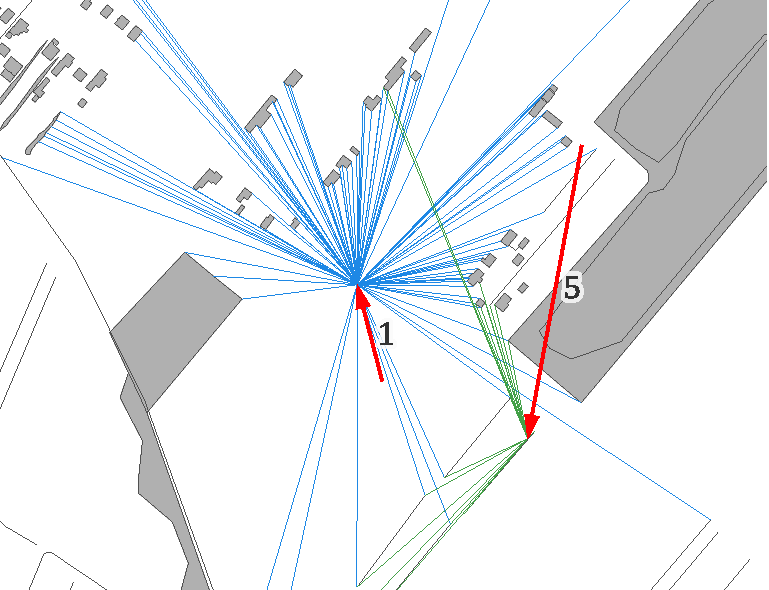
\includegraphics[width=\textwidth]{images/qgis-osm-rural}
				\end{minipage}
				\\
				\begin{minipage}[t]{0.4\textwidth}
					\captionof{table}[Statistics of routing requests with differently many visibility neighbors.]{Measured values for the first and fifth routing requests illustrated in \Cref{fig:eval-osm-rural-map}.}
				\end{minipage}
				\hfill
				\begin{minipage}[t]{0.56\textwidth}
					\captionof{figure}[Visualization of routing requests with differently many visibility neighbors.]{The first and fifth routing requests (red arrow between source and destination) with the nearby obstacles (gray). The bidirectional visibility edges of the two destinations are shown in blue and green.}
					\label{fig:eval-osm-rural-map}
				\end{minipage}
			\end{minipage}
			
			\clearpage
			\begin{figure}[h!]
				\begin{figcenter}
					\begin{subfigure}[t]{\textwidth}
						\begin{figcenter}
							\begingroup%
\makeatletter%
\begin{pgfpicture}%
\pgfpathrectangle{\pgfpointorigin}{\pgfqpoint{6.078790in}{1.733582in}}%
\pgfusepath{use as bounding box}%
\begin{pgfscope}%
\pgfsetbuttcap%
\pgfsetmiterjoin%
\definecolor{currentfill}{rgb}{1.000000,1.000000,1.000000}%
\pgfsetfillcolor{currentfill}%
\pgfsetlinewidth{0.000000pt}%
\definecolor{currentstroke}{rgb}{1.000000,1.000000,1.000000}%
\pgfsetstrokecolor{currentstroke}%
\pgfsetdash{}{0pt}%
\pgfpathmoveto{\pgfqpoint{0.000000in}{0.000000in}}%
\pgfpathlineto{\pgfqpoint{6.078790in}{0.000000in}}%
\pgfpathlineto{\pgfqpoint{6.078790in}{1.733582in}}%
\pgfpathlineto{\pgfqpoint{0.000000in}{1.733582in}}%
\pgfpathlineto{\pgfqpoint{0.000000in}{0.000000in}}%
\pgfpathclose%
\pgfusepath{fill}%
\end{pgfscope}%
\begin{pgfscope}%
\pgfsetbuttcap%
\pgfsetmiterjoin%
\definecolor{currentfill}{rgb}{1.000000,1.000000,1.000000}%
\pgfsetfillcolor{currentfill}%
\pgfsetlinewidth{0.000000pt}%
\definecolor{currentstroke}{rgb}{0.000000,0.000000,0.000000}%
\pgfsetstrokecolor{currentstroke}%
\pgfsetstrokeopacity{0.000000}%
\pgfsetdash{}{0pt}%
\pgfpathmoveto{\pgfqpoint{0.532932in}{0.451389in}}%
\pgfpathlineto{\pgfqpoint{5.094428in}{0.451389in}}%
\pgfpathlineto{\pgfqpoint{5.094428in}{1.665776in}}%
\pgfpathlineto{\pgfqpoint{0.532932in}{1.665776in}}%
\pgfpathlineto{\pgfqpoint{0.532932in}{0.451389in}}%
\pgfpathclose%
\pgfusepath{fill}%
\end{pgfscope}%
\begin{pgfscope}%
\pgfpathrectangle{\pgfqpoint{0.532932in}{0.451389in}}{\pgfqpoint{4.561496in}{1.214388in}}%
\pgfusepath{clip}%
\pgfsetroundcap%
\pgfsetroundjoin%
\pgfsetlinewidth{1.003750pt}%
\definecolor{currentstroke}{rgb}{0.800000,0.800000,0.800000}%
\pgfsetstrokecolor{currentstroke}%
\pgfsetdash{}{0pt}%
\pgfpathmoveto{\pgfqpoint{0.532932in}{0.451389in}}%
\pgfpathlineto{\pgfqpoint{0.532932in}{1.665776in}}%
\pgfusepath{stroke}%
\end{pgfscope}%
\begin{pgfscope}%
\definecolor{textcolor}{rgb}{0.150000,0.150000,0.150000}%
\pgfsetstrokecolor{textcolor}%
\pgfsetfillcolor{textcolor}%
\pgftext[x=0.532932in,y=0.319444in,,top]{\color{textcolor}\sffamily\fontsize{9.000000}{10.800000}\selectfont 0.0}%
\end{pgfscope}%
\begin{pgfscope}%
\pgfpathrectangle{\pgfqpoint{0.532932in}{0.451389in}}{\pgfqpoint{4.561496in}{1.214388in}}%
\pgfusepath{clip}%
\pgfsetroundcap%
\pgfsetroundjoin%
\pgfsetlinewidth{1.003750pt}%
\definecolor{currentstroke}{rgb}{0.800000,0.800000,0.800000}%
\pgfsetstrokecolor{currentstroke}%
\pgfsetdash{}{0pt}%
\pgfpathmoveto{\pgfqpoint{1.401742in}{0.451389in}}%
\pgfpathlineto{\pgfqpoint{1.401742in}{1.665776in}}%
\pgfusepath{stroke}%
\end{pgfscope}%
\begin{pgfscope}%
\definecolor{textcolor}{rgb}{0.150000,0.150000,0.150000}%
\pgfsetstrokecolor{textcolor}%
\pgfsetfillcolor{textcolor}%
\pgftext[x=1.401742in,y=0.319444in,,top]{\color{textcolor}\sffamily\fontsize{9.000000}{10.800000}\selectfont 0.5}%
\end{pgfscope}%
\begin{pgfscope}%
\pgfpathrectangle{\pgfqpoint{0.532932in}{0.451389in}}{\pgfqpoint{4.561496in}{1.214388in}}%
\pgfusepath{clip}%
\pgfsetroundcap%
\pgfsetroundjoin%
\pgfsetlinewidth{1.003750pt}%
\definecolor{currentstroke}{rgb}{0.800000,0.800000,0.800000}%
\pgfsetstrokecolor{currentstroke}%
\pgfsetdash{}{0pt}%
\pgfpathmoveto{\pgfqpoint{2.270552in}{0.451389in}}%
\pgfpathlineto{\pgfqpoint{2.270552in}{1.665776in}}%
\pgfusepath{stroke}%
\end{pgfscope}%
\begin{pgfscope}%
\definecolor{textcolor}{rgb}{0.150000,0.150000,0.150000}%
\pgfsetstrokecolor{textcolor}%
\pgfsetfillcolor{textcolor}%
\pgftext[x=2.270552in,y=0.319444in,,top]{\color{textcolor}\sffamily\fontsize{9.000000}{10.800000}\selectfont 1.0}%
\end{pgfscope}%
\begin{pgfscope}%
\pgfpathrectangle{\pgfqpoint{0.532932in}{0.451389in}}{\pgfqpoint{4.561496in}{1.214388in}}%
\pgfusepath{clip}%
\pgfsetroundcap%
\pgfsetroundjoin%
\pgfsetlinewidth{1.003750pt}%
\definecolor{currentstroke}{rgb}{0.800000,0.800000,0.800000}%
\pgfsetstrokecolor{currentstroke}%
\pgfsetdash{}{0pt}%
\pgfpathmoveto{\pgfqpoint{3.139362in}{0.451389in}}%
\pgfpathlineto{\pgfqpoint{3.139362in}{1.665776in}}%
\pgfusepath{stroke}%
\end{pgfscope}%
\begin{pgfscope}%
\definecolor{textcolor}{rgb}{0.150000,0.150000,0.150000}%
\pgfsetstrokecolor{textcolor}%
\pgfsetfillcolor{textcolor}%
\pgftext[x=3.139362in,y=0.319444in,,top]{\color{textcolor}\sffamily\fontsize{9.000000}{10.800000}\selectfont 1.5}%
\end{pgfscope}%
\begin{pgfscope}%
\pgfpathrectangle{\pgfqpoint{0.532932in}{0.451389in}}{\pgfqpoint{4.561496in}{1.214388in}}%
\pgfusepath{clip}%
\pgfsetroundcap%
\pgfsetroundjoin%
\pgfsetlinewidth{1.003750pt}%
\definecolor{currentstroke}{rgb}{0.800000,0.800000,0.800000}%
\pgfsetstrokecolor{currentstroke}%
\pgfsetdash{}{0pt}%
\pgfpathmoveto{\pgfqpoint{4.008172in}{0.451389in}}%
\pgfpathlineto{\pgfqpoint{4.008172in}{1.665776in}}%
\pgfusepath{stroke}%
\end{pgfscope}%
\begin{pgfscope}%
\definecolor{textcolor}{rgb}{0.150000,0.150000,0.150000}%
\pgfsetstrokecolor{textcolor}%
\pgfsetfillcolor{textcolor}%
\pgftext[x=4.008172in,y=0.319444in,,top]{\color{textcolor}\sffamily\fontsize{9.000000}{10.800000}\selectfont 2.0}%
\end{pgfscope}%
\begin{pgfscope}%
\pgfpathrectangle{\pgfqpoint{0.532932in}{0.451389in}}{\pgfqpoint{4.561496in}{1.214388in}}%
\pgfusepath{clip}%
\pgfsetroundcap%
\pgfsetroundjoin%
\pgfsetlinewidth{1.003750pt}%
\definecolor{currentstroke}{rgb}{0.800000,0.800000,0.800000}%
\pgfsetstrokecolor{currentstroke}%
\pgfsetdash{}{0pt}%
\pgfpathmoveto{\pgfqpoint{4.876983in}{0.451389in}}%
\pgfpathlineto{\pgfqpoint{4.876983in}{1.665776in}}%
\pgfusepath{stroke}%
\end{pgfscope}%
\begin{pgfscope}%
\definecolor{textcolor}{rgb}{0.150000,0.150000,0.150000}%
\pgfsetstrokecolor{textcolor}%
\pgfsetfillcolor{textcolor}%
\pgftext[x=4.876983in,y=0.319444in,,top]{\color{textcolor}\sffamily\fontsize{9.000000}{10.800000}\selectfont 2.5}%
\end{pgfscope}%
\begin{pgfscope}%
\definecolor{textcolor}{rgb}{0.150000,0.150000,0.150000}%
\pgfsetstrokecolor{textcolor}%
\pgfsetfillcolor{textcolor}%
\pgftext[x=2.813680in,y=0.125000in,,top]{\color{textcolor}\sffamily\fontsize{9.000000}{10.800000}\selectfont Beeline distance in km}%
\end{pgfscope}%
\begin{pgfscope}%
\pgfpathrectangle{\pgfqpoint{0.532932in}{0.451389in}}{\pgfqpoint{4.561496in}{1.214388in}}%
\pgfusepath{clip}%
\pgfsetroundcap%
\pgfsetroundjoin%
\pgfsetlinewidth{1.003750pt}%
\definecolor{currentstroke}{rgb}{0.800000,0.800000,0.800000}%
\pgfsetstrokecolor{currentstroke}%
\pgfsetdash{}{0pt}%
\pgfpathmoveto{\pgfqpoint{0.532932in}{0.451389in}}%
\pgfpathlineto{\pgfqpoint{5.094428in}{0.451389in}}%
\pgfusepath{stroke}%
\end{pgfscope}%
\begin{pgfscope}%
\definecolor{textcolor}{rgb}{0.150000,0.150000,0.150000}%
\pgfsetstrokecolor{textcolor}%
\pgfsetfillcolor{textcolor}%
\pgftext[x=0.332140in, y=0.403903in, left, base]{\color{textcolor}\sffamily\fontsize{9.000000}{10.800000}\selectfont 0}%
\end{pgfscope}%
\begin{pgfscope}%
\pgfpathrectangle{\pgfqpoint{0.532932in}{0.451389in}}{\pgfqpoint{4.561496in}{1.214388in}}%
\pgfusepath{clip}%
\pgfsetroundcap%
\pgfsetroundjoin%
\pgfsetlinewidth{1.003750pt}%
\definecolor{currentstroke}{rgb}{0.800000,0.800000,0.800000}%
\pgfsetstrokecolor{currentstroke}%
\pgfsetdash{}{0pt}%
\pgfpathmoveto{\pgfqpoint{0.532932in}{0.898454in}}%
\pgfpathlineto{\pgfqpoint{5.094428in}{0.898454in}}%
\pgfusepath{stroke}%
\end{pgfscope}%
\begin{pgfscope}%
\definecolor{textcolor}{rgb}{0.150000,0.150000,0.150000}%
\pgfsetstrokecolor{textcolor}%
\pgfsetfillcolor{textcolor}%
\pgftext[x=0.194444in, y=0.850969in, left, base]{\color{textcolor}\sffamily\fontsize{9.000000}{10.800000}\selectfont 200}%
\end{pgfscope}%
\begin{pgfscope}%
\pgfpathrectangle{\pgfqpoint{0.532932in}{0.451389in}}{\pgfqpoint{4.561496in}{1.214388in}}%
\pgfusepath{clip}%
\pgfsetroundcap%
\pgfsetroundjoin%
\pgfsetlinewidth{1.003750pt}%
\definecolor{currentstroke}{rgb}{0.800000,0.800000,0.800000}%
\pgfsetstrokecolor{currentstroke}%
\pgfsetdash{}{0pt}%
\pgfpathmoveto{\pgfqpoint{0.532932in}{1.345519in}}%
\pgfpathlineto{\pgfqpoint{5.094428in}{1.345519in}}%
\pgfusepath{stroke}%
\end{pgfscope}%
\begin{pgfscope}%
\definecolor{textcolor}{rgb}{0.150000,0.150000,0.150000}%
\pgfsetstrokecolor{textcolor}%
\pgfsetfillcolor{textcolor}%
\pgftext[x=0.194444in, y=1.298034in, left, base]{\color{textcolor}\sffamily\fontsize{9.000000}{10.800000}\selectfont 400}%
\end{pgfscope}%
\begin{pgfscope}%
\definecolor{textcolor}{rgb}{0.150000,0.150000,0.150000}%
\pgfsetstrokecolor{textcolor}%
\pgfsetfillcolor{textcolor}%
\pgftext[x=0.125000in,y=1.058583in,,bottom,rotate=90.000000]{\color{textcolor}\sffamily\fontsize{9.000000}{10.800000}\selectfont Average routing time in ms}%
\end{pgfscope}%
\begin{pgfscope}%
\pgfsetrectcap%
\pgfsetmiterjoin%
\pgfsetlinewidth{1.254687pt}%
\definecolor{currentstroke}{rgb}{0.800000,0.800000,0.800000}%
\pgfsetstrokecolor{currentstroke}%
\pgfsetdash{}{0pt}%
\pgfpathmoveto{\pgfqpoint{0.532932in}{0.451389in}}%
\pgfpathlineto{\pgfqpoint{0.532932in}{1.665776in}}%
\pgfusepath{stroke}%
\end{pgfscope}%
\begin{pgfscope}%
\pgfsetrectcap%
\pgfsetmiterjoin%
\pgfsetlinewidth{1.254687pt}%
\definecolor{currentstroke}{rgb}{0.800000,0.800000,0.800000}%
\pgfsetstrokecolor{currentstroke}%
\pgfsetdash{}{0pt}%
\pgfpathmoveto{\pgfqpoint{5.094428in}{0.451389in}}%
\pgfpathlineto{\pgfqpoint{5.094428in}{1.665776in}}%
\pgfusepath{stroke}%
\end{pgfscope}%
\begin{pgfscope}%
\pgfsetrectcap%
\pgfsetmiterjoin%
\pgfsetlinewidth{1.254687pt}%
\definecolor{currentstroke}{rgb}{0.800000,0.800000,0.800000}%
\pgfsetstrokecolor{currentstroke}%
\pgfsetdash{}{0pt}%
\pgfpathmoveto{\pgfqpoint{0.532932in}{0.451389in}}%
\pgfpathlineto{\pgfqpoint{5.094428in}{0.451389in}}%
\pgfusepath{stroke}%
\end{pgfscope}%
\begin{pgfscope}%
\pgfsetrectcap%
\pgfsetmiterjoin%
\pgfsetlinewidth{1.254687pt}%
\definecolor{currentstroke}{rgb}{0.800000,0.800000,0.800000}%
\pgfsetstrokecolor{currentstroke}%
\pgfsetdash{}{0pt}%
\pgfpathmoveto{\pgfqpoint{0.532932in}{1.665776in}}%
\pgfpathlineto{\pgfqpoint{5.094428in}{1.665776in}}%
\pgfusepath{stroke}%
\end{pgfscope}%
\begin{pgfscope}%
\pgfsetbuttcap%
\pgfsetmiterjoin%
\definecolor{currentfill}{rgb}{1.000000,1.000000,1.000000}%
\pgfsetfillcolor{currentfill}%
\pgfsetfillopacity{0.800000}%
\pgfsetlinewidth{1.003750pt}%
\definecolor{currentstroke}{rgb}{0.800000,0.800000,0.800000}%
\pgfsetstrokecolor{currentstroke}%
\pgfsetstrokeopacity{0.800000}%
\pgfsetdash{}{0pt}%
\pgfpathmoveto{\pgfqpoint{5.295965in}{0.383583in}}%
\pgfpathlineto{\pgfqpoint{6.053790in}{0.383583in}}%
\pgfpathquadraticcurveto{\pgfqpoint{6.078790in}{0.383583in}}{\pgfqpoint{6.078790in}{0.408583in}}%
\pgfpathlineto{\pgfqpoint{6.078790in}{1.708582in}}%
\pgfpathquadraticcurveto{\pgfqpoint{6.078790in}{1.733582in}}{\pgfqpoint{6.053790in}{1.733582in}}%
\pgfpathlineto{\pgfqpoint{5.295965in}{1.733582in}}%
\pgfpathquadraticcurveto{\pgfqpoint{5.270965in}{1.733582in}}{\pgfqpoint{5.270965in}{1.708582in}}%
\pgfpathlineto{\pgfqpoint{5.270965in}{0.408583in}}%
\pgfpathquadraticcurveto{\pgfqpoint{5.270965in}{0.383583in}}{\pgfqpoint{5.295965in}{0.383583in}}%
\pgfpathlineto{\pgfqpoint{5.295965in}{0.383583in}}%
\pgfpathclose%
\pgfusepath{stroke,fill}%
\end{pgfscope}%
\begin{pgfscope}%
\definecolor{textcolor}{rgb}{0.150000,0.150000,0.150000}%
\pgfsetstrokecolor{textcolor}%
\pgfsetfillcolor{textcolor}%
\pgftext[x=5.320965in,y=1.588611in,left,base]{\color{textcolor}\sffamily\fontsize{9.000000}{10.800000}\selectfont Vertex count}%
\end{pgfscope}%
\begin{pgfscope}%
\pgfsetroundcap%
\pgfsetroundjoin%
\pgfsetlinewidth{1.505625pt}%
\definecolor{currentstroke}{rgb}{0.003922,0.450980,0.698039}%
\pgfsetstrokecolor{currentstroke}%
\pgfsetdash{}{0pt}%
\pgfpathmoveto{\pgfqpoint{5.362182in}{1.444862in}}%
\pgfpathlineto{\pgfqpoint{5.487182in}{1.444862in}}%
\pgfpathlineto{\pgfqpoint{5.612182in}{1.444862in}}%
\pgfusepath{stroke}%
\end{pgfscope}%
\begin{pgfscope}%
\definecolor{textcolor}{rgb}{0.150000,0.150000,0.150000}%
\pgfsetstrokecolor{textcolor}%
\pgfsetfillcolor{textcolor}%
\pgftext[x=5.712182in,y=1.401112in,left,base]{\color{textcolor}\sffamily\fontsize{9.000000}{10.800000}\selectfont 370}%
\end{pgfscope}%
\begin{pgfscope}%
\pgfsetroundcap%
\pgfsetroundjoin%
\pgfsetlinewidth{1.505625pt}%
\definecolor{currentstroke}{rgb}{0.870588,0.560784,0.019608}%
\pgfsetstrokecolor{currentstroke}%
\pgfsetdash{}{0pt}%
\pgfpathmoveto{\pgfqpoint{5.362182in}{1.257362in}}%
\pgfpathlineto{\pgfqpoint{5.487182in}{1.257362in}}%
\pgfpathlineto{\pgfqpoint{5.612182in}{1.257362in}}%
\pgfusepath{stroke}%
\end{pgfscope}%
\begin{pgfscope}%
\definecolor{textcolor}{rgb}{0.150000,0.150000,0.150000}%
\pgfsetstrokecolor{textcolor}%
\pgfsetfillcolor{textcolor}%
\pgftext[x=5.712182in,y=1.213612in,left,base]{\color{textcolor}\sffamily\fontsize{9.000000}{10.800000}\selectfont 915}%
\end{pgfscope}%
\begin{pgfscope}%
\pgfsetroundcap%
\pgfsetroundjoin%
\pgfsetlinewidth{1.505625pt}%
\definecolor{currentstroke}{rgb}{0.007843,0.619608,0.450980}%
\pgfsetstrokecolor{currentstroke}%
\pgfsetdash{}{0pt}%
\pgfpathmoveto{\pgfqpoint{5.362182in}{1.069862in}}%
\pgfpathlineto{\pgfqpoint{5.487182in}{1.069862in}}%
\pgfpathlineto{\pgfqpoint{5.612182in}{1.069862in}}%
\pgfusepath{stroke}%
\end{pgfscope}%
\begin{pgfscope}%
\definecolor{textcolor}{rgb}{0.150000,0.150000,0.150000}%
\pgfsetstrokecolor{textcolor}%
\pgfsetfillcolor{textcolor}%
\pgftext[x=5.712182in,y=1.026112in,left,base]{\color{textcolor}\sffamily\fontsize{9.000000}{10.800000}\selectfont 1551}%
\end{pgfscope}%
\begin{pgfscope}%
\pgfsetroundcap%
\pgfsetroundjoin%
\pgfsetlinewidth{1.505625pt}%
\definecolor{currentstroke}{rgb}{0.835294,0.368627,0.000000}%
\pgfsetstrokecolor{currentstroke}%
\pgfsetdash{}{0pt}%
\pgfpathmoveto{\pgfqpoint{5.362182in}{0.882362in}}%
\pgfpathlineto{\pgfqpoint{5.487182in}{0.882362in}}%
\pgfpathlineto{\pgfqpoint{5.612182in}{0.882362in}}%
\pgfusepath{stroke}%
\end{pgfscope}%
\begin{pgfscope}%
\definecolor{textcolor}{rgb}{0.150000,0.150000,0.150000}%
\pgfsetstrokecolor{textcolor}%
\pgfsetfillcolor{textcolor}%
\pgftext[x=5.712182in,y=0.838612in,left,base]{\color{textcolor}\sffamily\fontsize{9.000000}{10.800000}\selectfont 2265}%
\end{pgfscope}%
\begin{pgfscope}%
\pgfsetroundcap%
\pgfsetroundjoin%
\pgfsetlinewidth{1.505625pt}%
\definecolor{currentstroke}{rgb}{0.800000,0.470588,0.737255}%
\pgfsetstrokecolor{currentstroke}%
\pgfsetdash{}{0pt}%
\pgfpathmoveto{\pgfqpoint{5.362182in}{0.694862in}}%
\pgfpathlineto{\pgfqpoint{5.487182in}{0.694862in}}%
\pgfpathlineto{\pgfqpoint{5.612182in}{0.694862in}}%
\pgfusepath{stroke}%
\end{pgfscope}%
\begin{pgfscope}%
\definecolor{textcolor}{rgb}{0.150000,0.150000,0.150000}%
\pgfsetstrokecolor{textcolor}%
\pgfsetfillcolor{textcolor}%
\pgftext[x=5.712182in,y=0.651112in,left,base]{\color{textcolor}\sffamily\fontsize{9.000000}{10.800000}\selectfont 4398}%
\end{pgfscope}%
\begin{pgfscope}%
\pgfsetroundcap%
\pgfsetroundjoin%
\pgfsetlinewidth{1.505625pt}%
\definecolor{currentstroke}{rgb}{0.792157,0.568627,0.380392}%
\pgfsetstrokecolor{currentstroke}%
\pgfsetdash{}{0pt}%
\pgfpathmoveto{\pgfqpoint{5.362182in}{0.507362in}}%
\pgfpathlineto{\pgfqpoint{5.487182in}{0.507362in}}%
\pgfpathlineto{\pgfqpoint{5.612182in}{0.507362in}}%
\pgfusepath{stroke}%
\end{pgfscope}%
\begin{pgfscope}%
\definecolor{textcolor}{rgb}{0.150000,0.150000,0.150000}%
\pgfsetstrokecolor{textcolor}%
\pgfsetfillcolor{textcolor}%
\pgftext[x=5.712182in,y=0.463612in,left,base]{\color{textcolor}\sffamily\fontsize{9.000000}{10.800000}\selectfont 6055}%
\end{pgfscope}%
\begin{pgfscope}%
\pgfsetroundcap%
\pgfsetroundjoin%
\pgfsetlinewidth{1.003750pt}%
\definecolor{currentstroke}{rgb}{0.003922,0.450980,0.698039}%
\pgfsetstrokecolor{currentstroke}%
\pgfsetdash{}{0pt}%
\pgfpathmoveto{\pgfqpoint{0.707425in}{0.869527in}}%
\pgfpathlineto{\pgfqpoint{0.795010in}{0.732629in}}%
\pgfpathlineto{\pgfqpoint{0.881627in}{0.697632in}}%
\pgfpathlineto{\pgfqpoint{0.968637in}{0.695690in}}%
\pgfpathlineto{\pgfqpoint{1.055570in}{0.554475in}}%
\pgfpathlineto{\pgfqpoint{1.142588in}{0.597072in}}%
\pgfpathlineto{\pgfqpoint{1.230777in}{0.732689in}}%
\pgfpathlineto{\pgfqpoint{1.316724in}{0.645701in}}%
\pgfpathlineto{\pgfqpoint{1.404053in}{0.598419in}}%
\pgfpathlineto{\pgfqpoint{1.491853in}{0.696682in}}%
\pgfpathlineto{\pgfqpoint{1.577891in}{0.773452in}}%
\pgfusepath{stroke}%
\end{pgfscope}%
\begin{pgfscope}%
\pgfsetbuttcap%
\pgfsetroundjoin%
\definecolor{currentfill}{rgb}{0.003922,0.450980,0.698039}%
\pgfsetfillcolor{currentfill}%
\pgfsetlinewidth{0.752812pt}%
\definecolor{currentstroke}{rgb}{1.000000,1.000000,1.000000}%
\pgfsetstrokecolor{currentstroke}%
\pgfsetdash{}{0pt}%
\pgfsys@defobject{currentmarker}{\pgfqpoint{-0.034722in}{-0.034722in}}{\pgfqpoint{0.034722in}{0.034722in}}{%
\pgfpathmoveto{\pgfqpoint{0.000000in}{-0.034722in}}%
\pgfpathcurveto{\pgfqpoint{0.009208in}{-0.034722in}}{\pgfqpoint{0.018041in}{-0.031064in}}{\pgfqpoint{0.024552in}{-0.024552in}}%
\pgfpathcurveto{\pgfqpoint{0.031064in}{-0.018041in}}{\pgfqpoint{0.034722in}{-0.009208in}}{\pgfqpoint{0.034722in}{0.000000in}}%
\pgfpathcurveto{\pgfqpoint{0.034722in}{0.009208in}}{\pgfqpoint{0.031064in}{0.018041in}}{\pgfqpoint{0.024552in}{0.024552in}}%
\pgfpathcurveto{\pgfqpoint{0.018041in}{0.031064in}}{\pgfqpoint{0.009208in}{0.034722in}}{\pgfqpoint{0.000000in}{0.034722in}}%
\pgfpathcurveto{\pgfqpoint{-0.009208in}{0.034722in}}{\pgfqpoint{-0.018041in}{0.031064in}}{\pgfqpoint{-0.024552in}{0.024552in}}%
\pgfpathcurveto{\pgfqpoint{-0.031064in}{0.018041in}}{\pgfqpoint{-0.034722in}{0.009208in}}{\pgfqpoint{-0.034722in}{0.000000in}}%
\pgfpathcurveto{\pgfqpoint{-0.034722in}{-0.009208in}}{\pgfqpoint{-0.031064in}{-0.018041in}}{\pgfqpoint{-0.024552in}{-0.024552in}}%
\pgfpathcurveto{\pgfqpoint{-0.018041in}{-0.031064in}}{\pgfqpoint{-0.009208in}{-0.034722in}}{\pgfqpoint{0.000000in}{-0.034722in}}%
\pgfpathlineto{\pgfqpoint{0.000000in}{-0.034722in}}%
\pgfpathclose%
\pgfusepath{stroke,fill}%
}%
\begin{pgfscope}%
\pgfsys@transformshift{0.707425in}{0.869527in}%
\pgfsys@useobject{currentmarker}{}%
\end{pgfscope}%
\begin{pgfscope}%
\pgfsys@transformshift{0.795010in}{0.732629in}%
\pgfsys@useobject{currentmarker}{}%
\end{pgfscope}%
\begin{pgfscope}%
\pgfsys@transformshift{0.881627in}{0.697632in}%
\pgfsys@useobject{currentmarker}{}%
\end{pgfscope}%
\begin{pgfscope}%
\pgfsys@transformshift{0.968637in}{0.695690in}%
\pgfsys@useobject{currentmarker}{}%
\end{pgfscope}%
\begin{pgfscope}%
\pgfsys@transformshift{1.055570in}{0.554475in}%
\pgfsys@useobject{currentmarker}{}%
\end{pgfscope}%
\begin{pgfscope}%
\pgfsys@transformshift{1.142588in}{0.597072in}%
\pgfsys@useobject{currentmarker}{}%
\end{pgfscope}%
\begin{pgfscope}%
\pgfsys@transformshift{1.230777in}{0.732689in}%
\pgfsys@useobject{currentmarker}{}%
\end{pgfscope}%
\begin{pgfscope}%
\pgfsys@transformshift{1.316724in}{0.645701in}%
\pgfsys@useobject{currentmarker}{}%
\end{pgfscope}%
\begin{pgfscope}%
\pgfsys@transformshift{1.404053in}{0.598419in}%
\pgfsys@useobject{currentmarker}{}%
\end{pgfscope}%
\begin{pgfscope}%
\pgfsys@transformshift{1.491853in}{0.696682in}%
\pgfsys@useobject{currentmarker}{}%
\end{pgfscope}%
\begin{pgfscope}%
\pgfsys@transformshift{1.577891in}{0.773452in}%
\pgfsys@useobject{currentmarker}{}%
\end{pgfscope}%
\end{pgfscope}%
\begin{pgfscope}%
\pgfsetroundcap%
\pgfsetroundjoin%
\pgfsetlinewidth{1.003750pt}%
\definecolor{currentstroke}{rgb}{0.870588,0.560784,0.019608}%
\pgfsetstrokecolor{currentstroke}%
\pgfsetdash{}{0pt}%
\pgfpathmoveto{\pgfqpoint{0.707425in}{1.303641in}}%
\pgfpathlineto{\pgfqpoint{0.795010in}{1.051227in}}%
\pgfpathlineto{\pgfqpoint{0.881627in}{0.986986in}}%
\pgfpathlineto{\pgfqpoint{0.968637in}{0.895783in}}%
\pgfpathlineto{\pgfqpoint{1.055570in}{0.618685in}}%
\pgfpathlineto{\pgfqpoint{1.142588in}{0.680116in}}%
\pgfpathlineto{\pgfqpoint{1.230777in}{0.959463in}}%
\pgfpathlineto{\pgfqpoint{1.316724in}{0.870727in}}%
\pgfpathlineto{\pgfqpoint{1.404053in}{0.746445in}}%
\pgfpathlineto{\pgfqpoint{1.491853in}{0.901856in}}%
\pgfpathlineto{\pgfqpoint{1.577891in}{1.103541in}}%
\pgfpathlineto{\pgfqpoint{1.665327in}{0.890740in}}%
\pgfpathlineto{\pgfqpoint{1.752647in}{0.581085in}}%
\pgfpathlineto{\pgfqpoint{1.838840in}{0.858683in}}%
\pgfpathlineto{\pgfqpoint{1.925918in}{0.938236in}}%
\pgfpathlineto{\pgfqpoint{2.014529in}{0.613790in}}%
\pgfpathlineto{\pgfqpoint{2.101363in}{0.551688in}}%
\pgfpathlineto{\pgfqpoint{2.188201in}{0.574973in}}%
\pgfpathlineto{\pgfqpoint{2.282396in}{0.568728in}}%
\pgfusepath{stroke}%
\end{pgfscope}%
\begin{pgfscope}%
\pgfsetbuttcap%
\pgfsetroundjoin%
\definecolor{currentfill}{rgb}{0.870588,0.560784,0.019608}%
\pgfsetfillcolor{currentfill}%
\pgfsetlinewidth{0.752812pt}%
\definecolor{currentstroke}{rgb}{1.000000,1.000000,1.000000}%
\pgfsetstrokecolor{currentstroke}%
\pgfsetdash{}{0pt}%
\pgfsys@defobject{currentmarker}{\pgfqpoint{-0.034722in}{-0.034722in}}{\pgfqpoint{0.034722in}{0.034722in}}{%
\pgfpathmoveto{\pgfqpoint{0.000000in}{-0.034722in}}%
\pgfpathcurveto{\pgfqpoint{0.009208in}{-0.034722in}}{\pgfqpoint{0.018041in}{-0.031064in}}{\pgfqpoint{0.024552in}{-0.024552in}}%
\pgfpathcurveto{\pgfqpoint{0.031064in}{-0.018041in}}{\pgfqpoint{0.034722in}{-0.009208in}}{\pgfqpoint{0.034722in}{0.000000in}}%
\pgfpathcurveto{\pgfqpoint{0.034722in}{0.009208in}}{\pgfqpoint{0.031064in}{0.018041in}}{\pgfqpoint{0.024552in}{0.024552in}}%
\pgfpathcurveto{\pgfqpoint{0.018041in}{0.031064in}}{\pgfqpoint{0.009208in}{0.034722in}}{\pgfqpoint{0.000000in}{0.034722in}}%
\pgfpathcurveto{\pgfqpoint{-0.009208in}{0.034722in}}{\pgfqpoint{-0.018041in}{0.031064in}}{\pgfqpoint{-0.024552in}{0.024552in}}%
\pgfpathcurveto{\pgfqpoint{-0.031064in}{0.018041in}}{\pgfqpoint{-0.034722in}{0.009208in}}{\pgfqpoint{-0.034722in}{0.000000in}}%
\pgfpathcurveto{\pgfqpoint{-0.034722in}{-0.009208in}}{\pgfqpoint{-0.031064in}{-0.018041in}}{\pgfqpoint{-0.024552in}{-0.024552in}}%
\pgfpathcurveto{\pgfqpoint{-0.018041in}{-0.031064in}}{\pgfqpoint{-0.009208in}{-0.034722in}}{\pgfqpoint{0.000000in}{-0.034722in}}%
\pgfpathlineto{\pgfqpoint{0.000000in}{-0.034722in}}%
\pgfpathclose%
\pgfusepath{stroke,fill}%
}%
\begin{pgfscope}%
\pgfsys@transformshift{0.707425in}{1.303641in}%
\pgfsys@useobject{currentmarker}{}%
\end{pgfscope}%
\begin{pgfscope}%
\pgfsys@transformshift{0.795010in}{1.051227in}%
\pgfsys@useobject{currentmarker}{}%
\end{pgfscope}%
\begin{pgfscope}%
\pgfsys@transformshift{0.881627in}{0.986986in}%
\pgfsys@useobject{currentmarker}{}%
\end{pgfscope}%
\begin{pgfscope}%
\pgfsys@transformshift{0.968637in}{0.895783in}%
\pgfsys@useobject{currentmarker}{}%
\end{pgfscope}%
\begin{pgfscope}%
\pgfsys@transformshift{1.055570in}{0.618685in}%
\pgfsys@useobject{currentmarker}{}%
\end{pgfscope}%
\begin{pgfscope}%
\pgfsys@transformshift{1.142588in}{0.680116in}%
\pgfsys@useobject{currentmarker}{}%
\end{pgfscope}%
\begin{pgfscope}%
\pgfsys@transformshift{1.230777in}{0.959463in}%
\pgfsys@useobject{currentmarker}{}%
\end{pgfscope}%
\begin{pgfscope}%
\pgfsys@transformshift{1.316724in}{0.870727in}%
\pgfsys@useobject{currentmarker}{}%
\end{pgfscope}%
\begin{pgfscope}%
\pgfsys@transformshift{1.404053in}{0.746445in}%
\pgfsys@useobject{currentmarker}{}%
\end{pgfscope}%
\begin{pgfscope}%
\pgfsys@transformshift{1.491853in}{0.901856in}%
\pgfsys@useobject{currentmarker}{}%
\end{pgfscope}%
\begin{pgfscope}%
\pgfsys@transformshift{1.577891in}{1.103541in}%
\pgfsys@useobject{currentmarker}{}%
\end{pgfscope}%
\begin{pgfscope}%
\pgfsys@transformshift{1.665327in}{0.890740in}%
\pgfsys@useobject{currentmarker}{}%
\end{pgfscope}%
\begin{pgfscope}%
\pgfsys@transformshift{1.752647in}{0.581085in}%
\pgfsys@useobject{currentmarker}{}%
\end{pgfscope}%
\begin{pgfscope}%
\pgfsys@transformshift{1.838840in}{0.858683in}%
\pgfsys@useobject{currentmarker}{}%
\end{pgfscope}%
\begin{pgfscope}%
\pgfsys@transformshift{1.925918in}{0.938236in}%
\pgfsys@useobject{currentmarker}{}%
\end{pgfscope}%
\begin{pgfscope}%
\pgfsys@transformshift{2.014529in}{0.613790in}%
\pgfsys@useobject{currentmarker}{}%
\end{pgfscope}%
\begin{pgfscope}%
\pgfsys@transformshift{2.101363in}{0.551688in}%
\pgfsys@useobject{currentmarker}{}%
\end{pgfscope}%
\begin{pgfscope}%
\pgfsys@transformshift{2.188201in}{0.574973in}%
\pgfsys@useobject{currentmarker}{}%
\end{pgfscope}%
\begin{pgfscope}%
\pgfsys@transformshift{2.282396in}{0.568728in}%
\pgfsys@useobject{currentmarker}{}%
\end{pgfscope}%
\end{pgfscope}%
\begin{pgfscope}%
\pgfsetroundcap%
\pgfsetroundjoin%
\pgfsetlinewidth{1.003750pt}%
\definecolor{currentstroke}{rgb}{0.007843,0.619608,0.450980}%
\pgfsetstrokecolor{currentstroke}%
\pgfsetdash{}{0pt}%
\pgfpathmoveto{\pgfqpoint{0.707425in}{1.330140in}}%
\pgfpathlineto{\pgfqpoint{0.795010in}{1.067438in}}%
\pgfpathlineto{\pgfqpoint{0.881627in}{1.014121in}}%
\pgfpathlineto{\pgfqpoint{0.968637in}{0.917682in}}%
\pgfpathlineto{\pgfqpoint{1.055570in}{0.625386in}}%
\pgfpathlineto{\pgfqpoint{1.142588in}{0.704477in}}%
\pgfpathlineto{\pgfqpoint{1.230777in}{0.991774in}}%
\pgfpathlineto{\pgfqpoint{1.316724in}{0.893930in}}%
\pgfpathlineto{\pgfqpoint{1.404053in}{0.766858in}}%
\pgfpathlineto{\pgfqpoint{1.491853in}{0.923402in}}%
\pgfpathlineto{\pgfqpoint{1.577891in}{1.139219in}}%
\pgfpathlineto{\pgfqpoint{1.665327in}{0.923738in}}%
\pgfpathlineto{\pgfqpoint{1.752647in}{0.590815in}}%
\pgfpathlineto{\pgfqpoint{1.838840in}{0.891062in}}%
\pgfpathlineto{\pgfqpoint{1.925918in}{0.974131in}}%
\pgfpathlineto{\pgfqpoint{2.014529in}{0.630172in}}%
\pgfpathlineto{\pgfqpoint{2.101363in}{0.699908in}}%
\pgfpathlineto{\pgfqpoint{2.188201in}{0.733594in}}%
\pgfpathlineto{\pgfqpoint{2.282396in}{0.585490in}}%
\pgfpathlineto{\pgfqpoint{2.354752in}{0.572686in}}%
\pgfpathlineto{\pgfqpoint{2.447051in}{0.549790in}}%
\pgfpathlineto{\pgfqpoint{2.543042in}{0.569423in}}%
\pgfpathlineto{\pgfqpoint{2.622057in}{0.598339in}}%
\pgfpathlineto{\pgfqpoint{2.700889in}{0.886743in}}%
\pgfpathlineto{\pgfqpoint{2.794273in}{0.853061in}}%
\pgfpathlineto{\pgfqpoint{3.143501in}{0.624519in}}%
\pgfusepath{stroke}%
\end{pgfscope}%
\begin{pgfscope}%
\pgfsetbuttcap%
\pgfsetroundjoin%
\definecolor{currentfill}{rgb}{0.007843,0.619608,0.450980}%
\pgfsetfillcolor{currentfill}%
\pgfsetlinewidth{0.752812pt}%
\definecolor{currentstroke}{rgb}{1.000000,1.000000,1.000000}%
\pgfsetstrokecolor{currentstroke}%
\pgfsetdash{}{0pt}%
\pgfsys@defobject{currentmarker}{\pgfqpoint{-0.034722in}{-0.034722in}}{\pgfqpoint{0.034722in}{0.034722in}}{%
\pgfpathmoveto{\pgfqpoint{0.000000in}{-0.034722in}}%
\pgfpathcurveto{\pgfqpoint{0.009208in}{-0.034722in}}{\pgfqpoint{0.018041in}{-0.031064in}}{\pgfqpoint{0.024552in}{-0.024552in}}%
\pgfpathcurveto{\pgfqpoint{0.031064in}{-0.018041in}}{\pgfqpoint{0.034722in}{-0.009208in}}{\pgfqpoint{0.034722in}{0.000000in}}%
\pgfpathcurveto{\pgfqpoint{0.034722in}{0.009208in}}{\pgfqpoint{0.031064in}{0.018041in}}{\pgfqpoint{0.024552in}{0.024552in}}%
\pgfpathcurveto{\pgfqpoint{0.018041in}{0.031064in}}{\pgfqpoint{0.009208in}{0.034722in}}{\pgfqpoint{0.000000in}{0.034722in}}%
\pgfpathcurveto{\pgfqpoint{-0.009208in}{0.034722in}}{\pgfqpoint{-0.018041in}{0.031064in}}{\pgfqpoint{-0.024552in}{0.024552in}}%
\pgfpathcurveto{\pgfqpoint{-0.031064in}{0.018041in}}{\pgfqpoint{-0.034722in}{0.009208in}}{\pgfqpoint{-0.034722in}{0.000000in}}%
\pgfpathcurveto{\pgfqpoint{-0.034722in}{-0.009208in}}{\pgfqpoint{-0.031064in}{-0.018041in}}{\pgfqpoint{-0.024552in}{-0.024552in}}%
\pgfpathcurveto{\pgfqpoint{-0.018041in}{-0.031064in}}{\pgfqpoint{-0.009208in}{-0.034722in}}{\pgfqpoint{0.000000in}{-0.034722in}}%
\pgfpathlineto{\pgfqpoint{0.000000in}{-0.034722in}}%
\pgfpathclose%
\pgfusepath{stroke,fill}%
}%
\begin{pgfscope}%
\pgfsys@transformshift{0.707425in}{1.330140in}%
\pgfsys@useobject{currentmarker}{}%
\end{pgfscope}%
\begin{pgfscope}%
\pgfsys@transformshift{0.795010in}{1.067438in}%
\pgfsys@useobject{currentmarker}{}%
\end{pgfscope}%
\begin{pgfscope}%
\pgfsys@transformshift{0.881627in}{1.014121in}%
\pgfsys@useobject{currentmarker}{}%
\end{pgfscope}%
\begin{pgfscope}%
\pgfsys@transformshift{0.968637in}{0.917682in}%
\pgfsys@useobject{currentmarker}{}%
\end{pgfscope}%
\begin{pgfscope}%
\pgfsys@transformshift{1.055570in}{0.625386in}%
\pgfsys@useobject{currentmarker}{}%
\end{pgfscope}%
\begin{pgfscope}%
\pgfsys@transformshift{1.142588in}{0.704477in}%
\pgfsys@useobject{currentmarker}{}%
\end{pgfscope}%
\begin{pgfscope}%
\pgfsys@transformshift{1.230777in}{0.991774in}%
\pgfsys@useobject{currentmarker}{}%
\end{pgfscope}%
\begin{pgfscope}%
\pgfsys@transformshift{1.316724in}{0.893930in}%
\pgfsys@useobject{currentmarker}{}%
\end{pgfscope}%
\begin{pgfscope}%
\pgfsys@transformshift{1.404053in}{0.766858in}%
\pgfsys@useobject{currentmarker}{}%
\end{pgfscope}%
\begin{pgfscope}%
\pgfsys@transformshift{1.491853in}{0.923402in}%
\pgfsys@useobject{currentmarker}{}%
\end{pgfscope}%
\begin{pgfscope}%
\pgfsys@transformshift{1.577891in}{1.139219in}%
\pgfsys@useobject{currentmarker}{}%
\end{pgfscope}%
\begin{pgfscope}%
\pgfsys@transformshift{1.665327in}{0.923738in}%
\pgfsys@useobject{currentmarker}{}%
\end{pgfscope}%
\begin{pgfscope}%
\pgfsys@transformshift{1.752647in}{0.590815in}%
\pgfsys@useobject{currentmarker}{}%
\end{pgfscope}%
\begin{pgfscope}%
\pgfsys@transformshift{1.838840in}{0.891062in}%
\pgfsys@useobject{currentmarker}{}%
\end{pgfscope}%
\begin{pgfscope}%
\pgfsys@transformshift{1.925918in}{0.974131in}%
\pgfsys@useobject{currentmarker}{}%
\end{pgfscope}%
\begin{pgfscope}%
\pgfsys@transformshift{2.014529in}{0.630172in}%
\pgfsys@useobject{currentmarker}{}%
\end{pgfscope}%
\begin{pgfscope}%
\pgfsys@transformshift{2.101363in}{0.699908in}%
\pgfsys@useobject{currentmarker}{}%
\end{pgfscope}%
\begin{pgfscope}%
\pgfsys@transformshift{2.188201in}{0.733594in}%
\pgfsys@useobject{currentmarker}{}%
\end{pgfscope}%
\begin{pgfscope}%
\pgfsys@transformshift{2.282396in}{0.585490in}%
\pgfsys@useobject{currentmarker}{}%
\end{pgfscope}%
\begin{pgfscope}%
\pgfsys@transformshift{2.354752in}{0.572686in}%
\pgfsys@useobject{currentmarker}{}%
\end{pgfscope}%
\begin{pgfscope}%
\pgfsys@transformshift{2.447051in}{0.549790in}%
\pgfsys@useobject{currentmarker}{}%
\end{pgfscope}%
\begin{pgfscope}%
\pgfsys@transformshift{2.543042in}{0.569423in}%
\pgfsys@useobject{currentmarker}{}%
\end{pgfscope}%
\begin{pgfscope}%
\pgfsys@transformshift{2.622057in}{0.598339in}%
\pgfsys@useobject{currentmarker}{}%
\end{pgfscope}%
\begin{pgfscope}%
\pgfsys@transformshift{2.700889in}{0.886743in}%
\pgfsys@useobject{currentmarker}{}%
\end{pgfscope}%
\begin{pgfscope}%
\pgfsys@transformshift{2.794273in}{0.853061in}%
\pgfsys@useobject{currentmarker}{}%
\end{pgfscope}%
\begin{pgfscope}%
\pgfsys@transformshift{3.143501in}{0.624519in}%
\pgfsys@useobject{currentmarker}{}%
\end{pgfscope}%
\end{pgfscope}%
\begin{pgfscope}%
\pgfsetroundcap%
\pgfsetroundjoin%
\pgfsetlinewidth{1.003750pt}%
\definecolor{currentstroke}{rgb}{0.835294,0.368627,0.000000}%
\pgfsetstrokecolor{currentstroke}%
\pgfsetdash{}{0pt}%
\pgfpathmoveto{\pgfqpoint{0.707425in}{1.397962in}}%
\pgfpathlineto{\pgfqpoint{0.795010in}{1.109078in}}%
\pgfpathlineto{\pgfqpoint{0.881627in}{1.052703in}}%
\pgfpathlineto{\pgfqpoint{0.968637in}{0.967519in}}%
\pgfpathlineto{\pgfqpoint{1.055570in}{0.652380in}}%
\pgfpathlineto{\pgfqpoint{1.142588in}{0.734613in}}%
\pgfpathlineto{\pgfqpoint{1.230777in}{1.048898in}}%
\pgfpathlineto{\pgfqpoint{1.316724in}{0.938448in}}%
\pgfpathlineto{\pgfqpoint{1.404053in}{0.807970in}}%
\pgfpathlineto{\pgfqpoint{1.491853in}{0.967968in}}%
\pgfpathlineto{\pgfqpoint{1.577891in}{1.195538in}}%
\pgfpathlineto{\pgfqpoint{1.665327in}{0.977059in}}%
\pgfpathlineto{\pgfqpoint{1.752647in}{0.635580in}}%
\pgfpathlineto{\pgfqpoint{1.838840in}{0.942345in}}%
\pgfpathlineto{\pgfqpoint{1.925918in}{1.015156in}}%
\pgfpathlineto{\pgfqpoint{2.014529in}{0.642015in}}%
\pgfpathlineto{\pgfqpoint{2.101363in}{0.741319in}}%
\pgfpathlineto{\pgfqpoint{2.188201in}{0.763302in}}%
\pgfpathlineto{\pgfqpoint{2.282396in}{0.606301in}}%
\pgfpathlineto{\pgfqpoint{2.354752in}{0.599526in}}%
\pgfpathlineto{\pgfqpoint{2.447051in}{0.575147in}}%
\pgfpathlineto{\pgfqpoint{2.543042in}{0.596857in}}%
\pgfpathlineto{\pgfqpoint{2.622057in}{0.627204in}}%
\pgfpathlineto{\pgfqpoint{2.700889in}{0.948391in}}%
\pgfpathlineto{\pgfqpoint{2.794273in}{0.898682in}}%
\pgfpathlineto{\pgfqpoint{3.143501in}{0.682039in}}%
\pgfusepath{stroke}%
\end{pgfscope}%
\begin{pgfscope}%
\pgfsetbuttcap%
\pgfsetroundjoin%
\definecolor{currentfill}{rgb}{0.835294,0.368627,0.000000}%
\pgfsetfillcolor{currentfill}%
\pgfsetlinewidth{0.752812pt}%
\definecolor{currentstroke}{rgb}{1.000000,1.000000,1.000000}%
\pgfsetstrokecolor{currentstroke}%
\pgfsetdash{}{0pt}%
\pgfsys@defobject{currentmarker}{\pgfqpoint{-0.034722in}{-0.034722in}}{\pgfqpoint{0.034722in}{0.034722in}}{%
\pgfpathmoveto{\pgfqpoint{0.000000in}{-0.034722in}}%
\pgfpathcurveto{\pgfqpoint{0.009208in}{-0.034722in}}{\pgfqpoint{0.018041in}{-0.031064in}}{\pgfqpoint{0.024552in}{-0.024552in}}%
\pgfpathcurveto{\pgfqpoint{0.031064in}{-0.018041in}}{\pgfqpoint{0.034722in}{-0.009208in}}{\pgfqpoint{0.034722in}{0.000000in}}%
\pgfpathcurveto{\pgfqpoint{0.034722in}{0.009208in}}{\pgfqpoint{0.031064in}{0.018041in}}{\pgfqpoint{0.024552in}{0.024552in}}%
\pgfpathcurveto{\pgfqpoint{0.018041in}{0.031064in}}{\pgfqpoint{0.009208in}{0.034722in}}{\pgfqpoint{0.000000in}{0.034722in}}%
\pgfpathcurveto{\pgfqpoint{-0.009208in}{0.034722in}}{\pgfqpoint{-0.018041in}{0.031064in}}{\pgfqpoint{-0.024552in}{0.024552in}}%
\pgfpathcurveto{\pgfqpoint{-0.031064in}{0.018041in}}{\pgfqpoint{-0.034722in}{0.009208in}}{\pgfqpoint{-0.034722in}{0.000000in}}%
\pgfpathcurveto{\pgfqpoint{-0.034722in}{-0.009208in}}{\pgfqpoint{-0.031064in}{-0.018041in}}{\pgfqpoint{-0.024552in}{-0.024552in}}%
\pgfpathcurveto{\pgfqpoint{-0.018041in}{-0.031064in}}{\pgfqpoint{-0.009208in}{-0.034722in}}{\pgfqpoint{0.000000in}{-0.034722in}}%
\pgfpathlineto{\pgfqpoint{0.000000in}{-0.034722in}}%
\pgfpathclose%
\pgfusepath{stroke,fill}%
}%
\begin{pgfscope}%
\pgfsys@transformshift{0.707425in}{1.397962in}%
\pgfsys@useobject{currentmarker}{}%
\end{pgfscope}%
\begin{pgfscope}%
\pgfsys@transformshift{0.795010in}{1.109078in}%
\pgfsys@useobject{currentmarker}{}%
\end{pgfscope}%
\begin{pgfscope}%
\pgfsys@transformshift{0.881627in}{1.052703in}%
\pgfsys@useobject{currentmarker}{}%
\end{pgfscope}%
\begin{pgfscope}%
\pgfsys@transformshift{0.968637in}{0.967519in}%
\pgfsys@useobject{currentmarker}{}%
\end{pgfscope}%
\begin{pgfscope}%
\pgfsys@transformshift{1.055570in}{0.652380in}%
\pgfsys@useobject{currentmarker}{}%
\end{pgfscope}%
\begin{pgfscope}%
\pgfsys@transformshift{1.142588in}{0.734613in}%
\pgfsys@useobject{currentmarker}{}%
\end{pgfscope}%
\begin{pgfscope}%
\pgfsys@transformshift{1.230777in}{1.048898in}%
\pgfsys@useobject{currentmarker}{}%
\end{pgfscope}%
\begin{pgfscope}%
\pgfsys@transformshift{1.316724in}{0.938448in}%
\pgfsys@useobject{currentmarker}{}%
\end{pgfscope}%
\begin{pgfscope}%
\pgfsys@transformshift{1.404053in}{0.807970in}%
\pgfsys@useobject{currentmarker}{}%
\end{pgfscope}%
\begin{pgfscope}%
\pgfsys@transformshift{1.491853in}{0.967968in}%
\pgfsys@useobject{currentmarker}{}%
\end{pgfscope}%
\begin{pgfscope}%
\pgfsys@transformshift{1.577891in}{1.195538in}%
\pgfsys@useobject{currentmarker}{}%
\end{pgfscope}%
\begin{pgfscope}%
\pgfsys@transformshift{1.665327in}{0.977059in}%
\pgfsys@useobject{currentmarker}{}%
\end{pgfscope}%
\begin{pgfscope}%
\pgfsys@transformshift{1.752647in}{0.635580in}%
\pgfsys@useobject{currentmarker}{}%
\end{pgfscope}%
\begin{pgfscope}%
\pgfsys@transformshift{1.838840in}{0.942345in}%
\pgfsys@useobject{currentmarker}{}%
\end{pgfscope}%
\begin{pgfscope}%
\pgfsys@transformshift{1.925918in}{1.015156in}%
\pgfsys@useobject{currentmarker}{}%
\end{pgfscope}%
\begin{pgfscope}%
\pgfsys@transformshift{2.014529in}{0.642015in}%
\pgfsys@useobject{currentmarker}{}%
\end{pgfscope}%
\begin{pgfscope}%
\pgfsys@transformshift{2.101363in}{0.741319in}%
\pgfsys@useobject{currentmarker}{}%
\end{pgfscope}%
\begin{pgfscope}%
\pgfsys@transformshift{2.188201in}{0.763302in}%
\pgfsys@useobject{currentmarker}{}%
\end{pgfscope}%
\begin{pgfscope}%
\pgfsys@transformshift{2.282396in}{0.606301in}%
\pgfsys@useobject{currentmarker}{}%
\end{pgfscope}%
\begin{pgfscope}%
\pgfsys@transformshift{2.354752in}{0.599526in}%
\pgfsys@useobject{currentmarker}{}%
\end{pgfscope}%
\begin{pgfscope}%
\pgfsys@transformshift{2.447051in}{0.575147in}%
\pgfsys@useobject{currentmarker}{}%
\end{pgfscope}%
\begin{pgfscope}%
\pgfsys@transformshift{2.543042in}{0.596857in}%
\pgfsys@useobject{currentmarker}{}%
\end{pgfscope}%
\begin{pgfscope}%
\pgfsys@transformshift{2.622057in}{0.627204in}%
\pgfsys@useobject{currentmarker}{}%
\end{pgfscope}%
\begin{pgfscope}%
\pgfsys@transformshift{2.700889in}{0.948391in}%
\pgfsys@useobject{currentmarker}{}%
\end{pgfscope}%
\begin{pgfscope}%
\pgfsys@transformshift{2.794273in}{0.898682in}%
\pgfsys@useobject{currentmarker}{}%
\end{pgfscope}%
\begin{pgfscope}%
\pgfsys@transformshift{3.143501in}{0.682039in}%
\pgfsys@useobject{currentmarker}{}%
\end{pgfscope}%
\end{pgfscope}%
\begin{pgfscope}%
\pgfsetroundcap%
\pgfsetroundjoin%
\pgfsetlinewidth{1.003750pt}%
\definecolor{currentstroke}{rgb}{0.800000,0.470588,0.737255}%
\pgfsetstrokecolor{currentstroke}%
\pgfsetdash{}{0pt}%
\pgfpathmoveto{\pgfqpoint{0.707425in}{1.472864in}}%
\pgfpathlineto{\pgfqpoint{0.795010in}{1.165462in}}%
\pgfpathlineto{\pgfqpoint{0.881627in}{1.113705in}}%
\pgfpathlineto{\pgfqpoint{0.968637in}{1.018140in}}%
\pgfpathlineto{\pgfqpoint{1.055570in}{0.692683in}}%
\pgfpathlineto{\pgfqpoint{1.142588in}{0.777009in}}%
\pgfpathlineto{\pgfqpoint{1.230777in}{1.097025in}}%
\pgfpathlineto{\pgfqpoint{1.316724in}{1.022269in}}%
\pgfpathlineto{\pgfqpoint{1.404053in}{0.881387in}}%
\pgfpathlineto{\pgfqpoint{1.491853in}{1.019412in}}%
\pgfpathlineto{\pgfqpoint{1.577891in}{1.250078in}}%
\pgfpathlineto{\pgfqpoint{1.665327in}{1.052821in}}%
\pgfpathlineto{\pgfqpoint{1.752647in}{0.753797in}}%
\pgfpathlineto{\pgfqpoint{1.838840in}{1.027423in}}%
\pgfpathlineto{\pgfqpoint{1.925918in}{1.065911in}}%
\pgfpathlineto{\pgfqpoint{2.014529in}{0.694404in}}%
\pgfpathlineto{\pgfqpoint{2.101363in}{0.875039in}}%
\pgfpathlineto{\pgfqpoint{2.188201in}{0.850973in}}%
\pgfpathlineto{\pgfqpoint{2.282396in}{0.663993in}}%
\pgfpathlineto{\pgfqpoint{2.354752in}{0.714634in}}%
\pgfpathlineto{\pgfqpoint{2.447051in}{0.667648in}}%
\pgfpathlineto{\pgfqpoint{2.543042in}{0.703639in}}%
\pgfpathlineto{\pgfqpoint{2.622057in}{0.720041in}}%
\pgfpathlineto{\pgfqpoint{2.700889in}{1.091573in}}%
\pgfpathlineto{\pgfqpoint{2.794273in}{0.966500in}}%
\pgfpathlineto{\pgfqpoint{3.143501in}{0.817173in}}%
\pgfpathlineto{\pgfqpoint{3.326970in}{0.814810in}}%
\pgfpathlineto{\pgfqpoint{3.492238in}{0.681272in}}%
\pgfpathlineto{\pgfqpoint{3.664367in}{0.779834in}}%
\pgfpathlineto{\pgfqpoint{3.847331in}{0.750283in}}%
\pgfpathlineto{\pgfqpoint{4.022061in}{0.653122in}}%
\pgfusepath{stroke}%
\end{pgfscope}%
\begin{pgfscope}%
\pgfsetbuttcap%
\pgfsetroundjoin%
\definecolor{currentfill}{rgb}{0.800000,0.470588,0.737255}%
\pgfsetfillcolor{currentfill}%
\pgfsetlinewidth{0.752812pt}%
\definecolor{currentstroke}{rgb}{1.000000,1.000000,1.000000}%
\pgfsetstrokecolor{currentstroke}%
\pgfsetdash{}{0pt}%
\pgfsys@defobject{currentmarker}{\pgfqpoint{-0.034722in}{-0.034722in}}{\pgfqpoint{0.034722in}{0.034722in}}{%
\pgfpathmoveto{\pgfqpoint{0.000000in}{-0.034722in}}%
\pgfpathcurveto{\pgfqpoint{0.009208in}{-0.034722in}}{\pgfqpoint{0.018041in}{-0.031064in}}{\pgfqpoint{0.024552in}{-0.024552in}}%
\pgfpathcurveto{\pgfqpoint{0.031064in}{-0.018041in}}{\pgfqpoint{0.034722in}{-0.009208in}}{\pgfqpoint{0.034722in}{0.000000in}}%
\pgfpathcurveto{\pgfqpoint{0.034722in}{0.009208in}}{\pgfqpoint{0.031064in}{0.018041in}}{\pgfqpoint{0.024552in}{0.024552in}}%
\pgfpathcurveto{\pgfqpoint{0.018041in}{0.031064in}}{\pgfqpoint{0.009208in}{0.034722in}}{\pgfqpoint{0.000000in}{0.034722in}}%
\pgfpathcurveto{\pgfqpoint{-0.009208in}{0.034722in}}{\pgfqpoint{-0.018041in}{0.031064in}}{\pgfqpoint{-0.024552in}{0.024552in}}%
\pgfpathcurveto{\pgfqpoint{-0.031064in}{0.018041in}}{\pgfqpoint{-0.034722in}{0.009208in}}{\pgfqpoint{-0.034722in}{0.000000in}}%
\pgfpathcurveto{\pgfqpoint{-0.034722in}{-0.009208in}}{\pgfqpoint{-0.031064in}{-0.018041in}}{\pgfqpoint{-0.024552in}{-0.024552in}}%
\pgfpathcurveto{\pgfqpoint{-0.018041in}{-0.031064in}}{\pgfqpoint{-0.009208in}{-0.034722in}}{\pgfqpoint{0.000000in}{-0.034722in}}%
\pgfpathlineto{\pgfqpoint{0.000000in}{-0.034722in}}%
\pgfpathclose%
\pgfusepath{stroke,fill}%
}%
\begin{pgfscope}%
\pgfsys@transformshift{0.707425in}{1.472864in}%
\pgfsys@useobject{currentmarker}{}%
\end{pgfscope}%
\begin{pgfscope}%
\pgfsys@transformshift{0.795010in}{1.165462in}%
\pgfsys@useobject{currentmarker}{}%
\end{pgfscope}%
\begin{pgfscope}%
\pgfsys@transformshift{0.881627in}{1.113705in}%
\pgfsys@useobject{currentmarker}{}%
\end{pgfscope}%
\begin{pgfscope}%
\pgfsys@transformshift{0.968637in}{1.018140in}%
\pgfsys@useobject{currentmarker}{}%
\end{pgfscope}%
\begin{pgfscope}%
\pgfsys@transformshift{1.055570in}{0.692683in}%
\pgfsys@useobject{currentmarker}{}%
\end{pgfscope}%
\begin{pgfscope}%
\pgfsys@transformshift{1.142588in}{0.777009in}%
\pgfsys@useobject{currentmarker}{}%
\end{pgfscope}%
\begin{pgfscope}%
\pgfsys@transformshift{1.230777in}{1.097025in}%
\pgfsys@useobject{currentmarker}{}%
\end{pgfscope}%
\begin{pgfscope}%
\pgfsys@transformshift{1.316724in}{1.022269in}%
\pgfsys@useobject{currentmarker}{}%
\end{pgfscope}%
\begin{pgfscope}%
\pgfsys@transformshift{1.404053in}{0.881387in}%
\pgfsys@useobject{currentmarker}{}%
\end{pgfscope}%
\begin{pgfscope}%
\pgfsys@transformshift{1.491853in}{1.019412in}%
\pgfsys@useobject{currentmarker}{}%
\end{pgfscope}%
\begin{pgfscope}%
\pgfsys@transformshift{1.577891in}{1.250078in}%
\pgfsys@useobject{currentmarker}{}%
\end{pgfscope}%
\begin{pgfscope}%
\pgfsys@transformshift{1.665327in}{1.052821in}%
\pgfsys@useobject{currentmarker}{}%
\end{pgfscope}%
\begin{pgfscope}%
\pgfsys@transformshift{1.752647in}{0.753797in}%
\pgfsys@useobject{currentmarker}{}%
\end{pgfscope}%
\begin{pgfscope}%
\pgfsys@transformshift{1.838840in}{1.027423in}%
\pgfsys@useobject{currentmarker}{}%
\end{pgfscope}%
\begin{pgfscope}%
\pgfsys@transformshift{1.925918in}{1.065911in}%
\pgfsys@useobject{currentmarker}{}%
\end{pgfscope}%
\begin{pgfscope}%
\pgfsys@transformshift{2.014529in}{0.694404in}%
\pgfsys@useobject{currentmarker}{}%
\end{pgfscope}%
\begin{pgfscope}%
\pgfsys@transformshift{2.101363in}{0.875039in}%
\pgfsys@useobject{currentmarker}{}%
\end{pgfscope}%
\begin{pgfscope}%
\pgfsys@transformshift{2.188201in}{0.850973in}%
\pgfsys@useobject{currentmarker}{}%
\end{pgfscope}%
\begin{pgfscope}%
\pgfsys@transformshift{2.282396in}{0.663993in}%
\pgfsys@useobject{currentmarker}{}%
\end{pgfscope}%
\begin{pgfscope}%
\pgfsys@transformshift{2.354752in}{0.714634in}%
\pgfsys@useobject{currentmarker}{}%
\end{pgfscope}%
\begin{pgfscope}%
\pgfsys@transformshift{2.447051in}{0.667648in}%
\pgfsys@useobject{currentmarker}{}%
\end{pgfscope}%
\begin{pgfscope}%
\pgfsys@transformshift{2.543042in}{0.703639in}%
\pgfsys@useobject{currentmarker}{}%
\end{pgfscope}%
\begin{pgfscope}%
\pgfsys@transformshift{2.622057in}{0.720041in}%
\pgfsys@useobject{currentmarker}{}%
\end{pgfscope}%
\begin{pgfscope}%
\pgfsys@transformshift{2.700889in}{1.091573in}%
\pgfsys@useobject{currentmarker}{}%
\end{pgfscope}%
\begin{pgfscope}%
\pgfsys@transformshift{2.794273in}{0.966500in}%
\pgfsys@useobject{currentmarker}{}%
\end{pgfscope}%
\begin{pgfscope}%
\pgfsys@transformshift{3.143501in}{0.817173in}%
\pgfsys@useobject{currentmarker}{}%
\end{pgfscope}%
\begin{pgfscope}%
\pgfsys@transformshift{3.326970in}{0.814810in}%
\pgfsys@useobject{currentmarker}{}%
\end{pgfscope}%
\begin{pgfscope}%
\pgfsys@transformshift{3.492238in}{0.681272in}%
\pgfsys@useobject{currentmarker}{}%
\end{pgfscope}%
\begin{pgfscope}%
\pgfsys@transformshift{3.664367in}{0.779834in}%
\pgfsys@useobject{currentmarker}{}%
\end{pgfscope}%
\begin{pgfscope}%
\pgfsys@transformshift{3.847331in}{0.750283in}%
\pgfsys@useobject{currentmarker}{}%
\end{pgfscope}%
\begin{pgfscope}%
\pgfsys@transformshift{4.022061in}{0.653122in}%
\pgfsys@useobject{currentmarker}{}%
\end{pgfscope}%
\end{pgfscope}%
\begin{pgfscope}%
\pgfsetroundcap%
\pgfsetroundjoin%
\pgfsetlinewidth{1.003750pt}%
\definecolor{currentstroke}{rgb}{0.792157,0.568627,0.380392}%
\pgfsetstrokecolor{currentstroke}%
\pgfsetdash{}{0pt}%
\pgfpathmoveto{\pgfqpoint{0.707425in}{1.612634in}}%
\pgfpathlineto{\pgfqpoint{0.795010in}{1.264931in}}%
\pgfpathlineto{\pgfqpoint{0.881627in}{1.197965in}}%
\pgfpathlineto{\pgfqpoint{0.968637in}{1.095992in}}%
\pgfpathlineto{\pgfqpoint{1.055570in}{0.735709in}}%
\pgfpathlineto{\pgfqpoint{1.142588in}{0.831533in}}%
\pgfpathlineto{\pgfqpoint{1.230777in}{1.185524in}}%
\pgfpathlineto{\pgfqpoint{1.316724in}{1.115549in}}%
\pgfpathlineto{\pgfqpoint{1.404053in}{0.956186in}}%
\pgfpathlineto{\pgfqpoint{1.491853in}{1.098446in}}%
\pgfpathlineto{\pgfqpoint{1.577891in}{1.363431in}}%
\pgfpathlineto{\pgfqpoint{1.665327in}{1.154298in}}%
\pgfpathlineto{\pgfqpoint{1.752647in}{0.837631in}}%
\pgfpathlineto{\pgfqpoint{1.838840in}{1.126120in}}%
\pgfpathlineto{\pgfqpoint{1.925918in}{1.159200in}}%
\pgfpathlineto{\pgfqpoint{2.014529in}{0.750035in}}%
\pgfpathlineto{\pgfqpoint{2.101363in}{0.970311in}}%
\pgfpathlineto{\pgfqpoint{2.188201in}{0.918306in}}%
\pgfpathlineto{\pgfqpoint{2.282396in}{0.723280in}}%
\pgfpathlineto{\pgfqpoint{2.354752in}{0.784662in}}%
\pgfpathlineto{\pgfqpoint{2.447051in}{0.707964in}}%
\pgfpathlineto{\pgfqpoint{2.543042in}{0.810907in}}%
\pgfpathlineto{\pgfqpoint{2.622057in}{0.779123in}}%
\pgfpathlineto{\pgfqpoint{2.700889in}{1.243606in}}%
\pgfpathlineto{\pgfqpoint{2.794273in}{1.112013in}}%
\pgfpathlineto{\pgfqpoint{3.143501in}{0.910775in}}%
\pgfpathlineto{\pgfqpoint{3.326970in}{0.871203in}}%
\pgfpathlineto{\pgfqpoint{3.492238in}{0.738011in}}%
\pgfpathlineto{\pgfqpoint{3.664367in}{0.877189in}}%
\pgfpathlineto{\pgfqpoint{3.847331in}{0.845817in}}%
\pgfpathlineto{\pgfqpoint{4.022061in}{0.756871in}}%
\pgfpathlineto{\pgfqpoint{4.184937in}{0.757190in}}%
\pgfpathlineto{\pgfqpoint{4.359820in}{0.757669in}}%
\pgfpathlineto{\pgfqpoint{4.544981in}{0.824498in}}%
\pgfpathlineto{\pgfqpoint{4.885523in}{0.862673in}}%
\pgfusepath{stroke}%
\end{pgfscope}%
\begin{pgfscope}%
\pgfsetbuttcap%
\pgfsetroundjoin%
\definecolor{currentfill}{rgb}{0.792157,0.568627,0.380392}%
\pgfsetfillcolor{currentfill}%
\pgfsetlinewidth{0.752812pt}%
\definecolor{currentstroke}{rgb}{1.000000,1.000000,1.000000}%
\pgfsetstrokecolor{currentstroke}%
\pgfsetdash{}{0pt}%
\pgfsys@defobject{currentmarker}{\pgfqpoint{-0.034722in}{-0.034722in}}{\pgfqpoint{0.034722in}{0.034722in}}{%
\pgfpathmoveto{\pgfqpoint{0.000000in}{-0.034722in}}%
\pgfpathcurveto{\pgfqpoint{0.009208in}{-0.034722in}}{\pgfqpoint{0.018041in}{-0.031064in}}{\pgfqpoint{0.024552in}{-0.024552in}}%
\pgfpathcurveto{\pgfqpoint{0.031064in}{-0.018041in}}{\pgfqpoint{0.034722in}{-0.009208in}}{\pgfqpoint{0.034722in}{0.000000in}}%
\pgfpathcurveto{\pgfqpoint{0.034722in}{0.009208in}}{\pgfqpoint{0.031064in}{0.018041in}}{\pgfqpoint{0.024552in}{0.024552in}}%
\pgfpathcurveto{\pgfqpoint{0.018041in}{0.031064in}}{\pgfqpoint{0.009208in}{0.034722in}}{\pgfqpoint{0.000000in}{0.034722in}}%
\pgfpathcurveto{\pgfqpoint{-0.009208in}{0.034722in}}{\pgfqpoint{-0.018041in}{0.031064in}}{\pgfqpoint{-0.024552in}{0.024552in}}%
\pgfpathcurveto{\pgfqpoint{-0.031064in}{0.018041in}}{\pgfqpoint{-0.034722in}{0.009208in}}{\pgfqpoint{-0.034722in}{0.000000in}}%
\pgfpathcurveto{\pgfqpoint{-0.034722in}{-0.009208in}}{\pgfqpoint{-0.031064in}{-0.018041in}}{\pgfqpoint{-0.024552in}{-0.024552in}}%
\pgfpathcurveto{\pgfqpoint{-0.018041in}{-0.031064in}}{\pgfqpoint{-0.009208in}{-0.034722in}}{\pgfqpoint{0.000000in}{-0.034722in}}%
\pgfpathlineto{\pgfqpoint{0.000000in}{-0.034722in}}%
\pgfpathclose%
\pgfusepath{stroke,fill}%
}%
\begin{pgfscope}%
\pgfsys@transformshift{0.707425in}{1.612634in}%
\pgfsys@useobject{currentmarker}{}%
\end{pgfscope}%
\begin{pgfscope}%
\pgfsys@transformshift{0.795010in}{1.264931in}%
\pgfsys@useobject{currentmarker}{}%
\end{pgfscope}%
\begin{pgfscope}%
\pgfsys@transformshift{0.881627in}{1.197965in}%
\pgfsys@useobject{currentmarker}{}%
\end{pgfscope}%
\begin{pgfscope}%
\pgfsys@transformshift{0.968637in}{1.095992in}%
\pgfsys@useobject{currentmarker}{}%
\end{pgfscope}%
\begin{pgfscope}%
\pgfsys@transformshift{1.055570in}{0.735709in}%
\pgfsys@useobject{currentmarker}{}%
\end{pgfscope}%
\begin{pgfscope}%
\pgfsys@transformshift{1.142588in}{0.831533in}%
\pgfsys@useobject{currentmarker}{}%
\end{pgfscope}%
\begin{pgfscope}%
\pgfsys@transformshift{1.230777in}{1.185524in}%
\pgfsys@useobject{currentmarker}{}%
\end{pgfscope}%
\begin{pgfscope}%
\pgfsys@transformshift{1.316724in}{1.115549in}%
\pgfsys@useobject{currentmarker}{}%
\end{pgfscope}%
\begin{pgfscope}%
\pgfsys@transformshift{1.404053in}{0.956186in}%
\pgfsys@useobject{currentmarker}{}%
\end{pgfscope}%
\begin{pgfscope}%
\pgfsys@transformshift{1.491853in}{1.098446in}%
\pgfsys@useobject{currentmarker}{}%
\end{pgfscope}%
\begin{pgfscope}%
\pgfsys@transformshift{1.577891in}{1.363431in}%
\pgfsys@useobject{currentmarker}{}%
\end{pgfscope}%
\begin{pgfscope}%
\pgfsys@transformshift{1.665327in}{1.154298in}%
\pgfsys@useobject{currentmarker}{}%
\end{pgfscope}%
\begin{pgfscope}%
\pgfsys@transformshift{1.752647in}{0.837631in}%
\pgfsys@useobject{currentmarker}{}%
\end{pgfscope}%
\begin{pgfscope}%
\pgfsys@transformshift{1.838840in}{1.126120in}%
\pgfsys@useobject{currentmarker}{}%
\end{pgfscope}%
\begin{pgfscope}%
\pgfsys@transformshift{1.925918in}{1.159200in}%
\pgfsys@useobject{currentmarker}{}%
\end{pgfscope}%
\begin{pgfscope}%
\pgfsys@transformshift{2.014529in}{0.750035in}%
\pgfsys@useobject{currentmarker}{}%
\end{pgfscope}%
\begin{pgfscope}%
\pgfsys@transformshift{2.101363in}{0.970311in}%
\pgfsys@useobject{currentmarker}{}%
\end{pgfscope}%
\begin{pgfscope}%
\pgfsys@transformshift{2.188201in}{0.918306in}%
\pgfsys@useobject{currentmarker}{}%
\end{pgfscope}%
\begin{pgfscope}%
\pgfsys@transformshift{2.282396in}{0.723280in}%
\pgfsys@useobject{currentmarker}{}%
\end{pgfscope}%
\begin{pgfscope}%
\pgfsys@transformshift{2.354752in}{0.784662in}%
\pgfsys@useobject{currentmarker}{}%
\end{pgfscope}%
\begin{pgfscope}%
\pgfsys@transformshift{2.447051in}{0.707964in}%
\pgfsys@useobject{currentmarker}{}%
\end{pgfscope}%
\begin{pgfscope}%
\pgfsys@transformshift{2.543042in}{0.810907in}%
\pgfsys@useobject{currentmarker}{}%
\end{pgfscope}%
\begin{pgfscope}%
\pgfsys@transformshift{2.622057in}{0.779123in}%
\pgfsys@useobject{currentmarker}{}%
\end{pgfscope}%
\begin{pgfscope}%
\pgfsys@transformshift{2.700889in}{1.243606in}%
\pgfsys@useobject{currentmarker}{}%
\end{pgfscope}%
\begin{pgfscope}%
\pgfsys@transformshift{2.794273in}{1.112013in}%
\pgfsys@useobject{currentmarker}{}%
\end{pgfscope}%
\begin{pgfscope}%
\pgfsys@transformshift{3.143501in}{0.910775in}%
\pgfsys@useobject{currentmarker}{}%
\end{pgfscope}%
\begin{pgfscope}%
\pgfsys@transformshift{3.326970in}{0.871203in}%
\pgfsys@useobject{currentmarker}{}%
\end{pgfscope}%
\begin{pgfscope}%
\pgfsys@transformshift{3.492238in}{0.738011in}%
\pgfsys@useobject{currentmarker}{}%
\end{pgfscope}%
\begin{pgfscope}%
\pgfsys@transformshift{3.664367in}{0.877189in}%
\pgfsys@useobject{currentmarker}{}%
\end{pgfscope}%
\begin{pgfscope}%
\pgfsys@transformshift{3.847331in}{0.845817in}%
\pgfsys@useobject{currentmarker}{}%
\end{pgfscope}%
\begin{pgfscope}%
\pgfsys@transformshift{4.022061in}{0.756871in}%
\pgfsys@useobject{currentmarker}{}%
\end{pgfscope}%
\begin{pgfscope}%
\pgfsys@transformshift{4.184937in}{0.757190in}%
\pgfsys@useobject{currentmarker}{}%
\end{pgfscope}%
\begin{pgfscope}%
\pgfsys@transformshift{4.359820in}{0.757669in}%
\pgfsys@useobject{currentmarker}{}%
\end{pgfscope}%
\begin{pgfscope}%
\pgfsys@transformshift{4.544981in}{0.824498in}%
\pgfsys@useobject{currentmarker}{}%
\end{pgfscope}%
\begin{pgfscope}%
\pgfsys@transformshift{4.885523in}{0.862673in}%
\pgfsys@useobject{currentmarker}{}%
\end{pgfscope}%
\end{pgfscope}%
\end{pgfpicture}%
\makeatother%
\endgroup%

						\end{figcenter}
						\caption{Total routing times of all datasets.}
						\label{fig:eval-city-routing-details-a}
					\end{subfigure}
					\\[3ex]
					\begin{subfigure}[t]{\textwidth}
						\begin{figcenter}
							\begingroup%
\makeatletter%
\begin{pgfpicture}%
\pgfpathrectangle{\pgfpointorigin}{\pgfqpoint{6.079644in}{1.715788in}}%
\pgfusepath{use as bounding box}%
\begin{pgfscope}%
\pgfsetbuttcap%
\pgfsetmiterjoin%
\definecolor{currentfill}{rgb}{1.000000,1.000000,1.000000}%
\pgfsetfillcolor{currentfill}%
\pgfsetlinewidth{0.000000pt}%
\definecolor{currentstroke}{rgb}{1.000000,1.000000,1.000000}%
\pgfsetstrokecolor{currentstroke}%
\pgfsetdash{}{0pt}%
\pgfpathmoveto{\pgfqpoint{0.000000in}{0.000000in}}%
\pgfpathlineto{\pgfqpoint{6.079644in}{0.000000in}}%
\pgfpathlineto{\pgfqpoint{6.079644in}{1.715788in}}%
\pgfpathlineto{\pgfqpoint{0.000000in}{1.715788in}}%
\pgfpathlineto{\pgfqpoint{0.000000in}{0.000000in}}%
\pgfpathclose%
\pgfusepath{fill}%
\end{pgfscope}%
\begin{pgfscope}%
\pgfsetbuttcap%
\pgfsetmiterjoin%
\definecolor{currentfill}{rgb}{1.000000,1.000000,1.000000}%
\pgfsetfillcolor{currentfill}%
\pgfsetlinewidth{0.000000pt}%
\definecolor{currentstroke}{rgb}{0.000000,0.000000,0.000000}%
\pgfsetstrokecolor{currentstroke}%
\pgfsetstrokeopacity{0.000000}%
\pgfsetdash{}{0pt}%
\pgfpathmoveto{\pgfqpoint{0.601779in}{0.451389in}}%
\pgfpathlineto{\pgfqpoint{4.376166in}{0.451389in}}%
\pgfpathlineto{\pgfqpoint{4.376166in}{1.715788in}}%
\pgfpathlineto{\pgfqpoint{0.601779in}{1.715788in}}%
\pgfpathlineto{\pgfqpoint{0.601779in}{0.451389in}}%
\pgfpathclose%
\pgfusepath{fill}%
\end{pgfscope}%
\begin{pgfscope}%
\pgfpathrectangle{\pgfqpoint{0.601779in}{0.451389in}}{\pgfqpoint{3.774387in}{1.264399in}}%
\pgfusepath{clip}%
\pgfsetroundcap%
\pgfsetroundjoin%
\pgfsetlinewidth{1.003750pt}%
\definecolor{currentstroke}{rgb}{0.800000,0.800000,0.800000}%
\pgfsetstrokecolor{currentstroke}%
\pgfsetdash{}{0pt}%
\pgfpathmoveto{\pgfqpoint{0.601779in}{0.451389in}}%
\pgfpathlineto{\pgfqpoint{0.601779in}{1.715788in}}%
\pgfusepath{stroke}%
\end{pgfscope}%
\begin{pgfscope}%
\definecolor{textcolor}{rgb}{0.150000,0.150000,0.150000}%
\pgfsetstrokecolor{textcolor}%
\pgfsetfillcolor{textcolor}%
\pgftext[x=0.601779in,y=0.319444in,,top]{\color{textcolor}\sffamily\fontsize{9.000000}{10.800000}\selectfont 0.0}%
\end{pgfscope}%
\begin{pgfscope}%
\pgfpathrectangle{\pgfqpoint{0.601779in}{0.451389in}}{\pgfqpoint{3.774387in}{1.264399in}}%
\pgfusepath{clip}%
\pgfsetroundcap%
\pgfsetroundjoin%
\pgfsetlinewidth{1.003750pt}%
\definecolor{currentstroke}{rgb}{0.800000,0.800000,0.800000}%
\pgfsetstrokecolor{currentstroke}%
\pgfsetdash{}{0pt}%
\pgfpathmoveto{\pgfqpoint{1.321582in}{0.451389in}}%
\pgfpathlineto{\pgfqpoint{1.321582in}{1.715788in}}%
\pgfusepath{stroke}%
\end{pgfscope}%
\begin{pgfscope}%
\definecolor{textcolor}{rgb}{0.150000,0.150000,0.150000}%
\pgfsetstrokecolor{textcolor}%
\pgfsetfillcolor{textcolor}%
\pgftext[x=1.321582in,y=0.319444in,,top]{\color{textcolor}\sffamily\fontsize{9.000000}{10.800000}\selectfont 0.5}%
\end{pgfscope}%
\begin{pgfscope}%
\pgfpathrectangle{\pgfqpoint{0.601779in}{0.451389in}}{\pgfqpoint{3.774387in}{1.264399in}}%
\pgfusepath{clip}%
\pgfsetroundcap%
\pgfsetroundjoin%
\pgfsetlinewidth{1.003750pt}%
\definecolor{currentstroke}{rgb}{0.800000,0.800000,0.800000}%
\pgfsetstrokecolor{currentstroke}%
\pgfsetdash{}{0pt}%
\pgfpathmoveto{\pgfqpoint{2.041385in}{0.451389in}}%
\pgfpathlineto{\pgfqpoint{2.041385in}{1.715788in}}%
\pgfusepath{stroke}%
\end{pgfscope}%
\begin{pgfscope}%
\definecolor{textcolor}{rgb}{0.150000,0.150000,0.150000}%
\pgfsetstrokecolor{textcolor}%
\pgfsetfillcolor{textcolor}%
\pgftext[x=2.041385in,y=0.319444in,,top]{\color{textcolor}\sffamily\fontsize{9.000000}{10.800000}\selectfont 1.0}%
\end{pgfscope}%
\begin{pgfscope}%
\pgfpathrectangle{\pgfqpoint{0.601779in}{0.451389in}}{\pgfqpoint{3.774387in}{1.264399in}}%
\pgfusepath{clip}%
\pgfsetroundcap%
\pgfsetroundjoin%
\pgfsetlinewidth{1.003750pt}%
\definecolor{currentstroke}{rgb}{0.800000,0.800000,0.800000}%
\pgfsetstrokecolor{currentstroke}%
\pgfsetdash{}{0pt}%
\pgfpathmoveto{\pgfqpoint{2.761188in}{0.451389in}}%
\pgfpathlineto{\pgfqpoint{2.761188in}{1.715788in}}%
\pgfusepath{stroke}%
\end{pgfscope}%
\begin{pgfscope}%
\definecolor{textcolor}{rgb}{0.150000,0.150000,0.150000}%
\pgfsetstrokecolor{textcolor}%
\pgfsetfillcolor{textcolor}%
\pgftext[x=2.761188in,y=0.319444in,,top]{\color{textcolor}\sffamily\fontsize{9.000000}{10.800000}\selectfont 1.5}%
\end{pgfscope}%
\begin{pgfscope}%
\pgfpathrectangle{\pgfqpoint{0.601779in}{0.451389in}}{\pgfqpoint{3.774387in}{1.264399in}}%
\pgfusepath{clip}%
\pgfsetroundcap%
\pgfsetroundjoin%
\pgfsetlinewidth{1.003750pt}%
\definecolor{currentstroke}{rgb}{0.800000,0.800000,0.800000}%
\pgfsetstrokecolor{currentstroke}%
\pgfsetdash{}{0pt}%
\pgfpathmoveto{\pgfqpoint{3.480991in}{0.451389in}}%
\pgfpathlineto{\pgfqpoint{3.480991in}{1.715788in}}%
\pgfusepath{stroke}%
\end{pgfscope}%
\begin{pgfscope}%
\definecolor{textcolor}{rgb}{0.150000,0.150000,0.150000}%
\pgfsetstrokecolor{textcolor}%
\pgfsetfillcolor{textcolor}%
\pgftext[x=3.480991in,y=0.319444in,,top]{\color{textcolor}\sffamily\fontsize{9.000000}{10.800000}\selectfont 2.0}%
\end{pgfscope}%
\begin{pgfscope}%
\pgfpathrectangle{\pgfqpoint{0.601779in}{0.451389in}}{\pgfqpoint{3.774387in}{1.264399in}}%
\pgfusepath{clip}%
\pgfsetroundcap%
\pgfsetroundjoin%
\pgfsetlinewidth{1.003750pt}%
\definecolor{currentstroke}{rgb}{0.800000,0.800000,0.800000}%
\pgfsetstrokecolor{currentstroke}%
\pgfsetdash{}{0pt}%
\pgfpathmoveto{\pgfqpoint{4.200794in}{0.451389in}}%
\pgfpathlineto{\pgfqpoint{4.200794in}{1.715788in}}%
\pgfusepath{stroke}%
\end{pgfscope}%
\begin{pgfscope}%
\definecolor{textcolor}{rgb}{0.150000,0.150000,0.150000}%
\pgfsetstrokecolor{textcolor}%
\pgfsetfillcolor{textcolor}%
\pgftext[x=4.200794in,y=0.319444in,,top]{\color{textcolor}\sffamily\fontsize{9.000000}{10.800000}\selectfont 2.5}%
\end{pgfscope}%
\begin{pgfscope}%
\definecolor{textcolor}{rgb}{0.150000,0.150000,0.150000}%
\pgfsetstrokecolor{textcolor}%
\pgfsetfillcolor{textcolor}%
\pgftext[x=2.488973in,y=0.125000in,,top]{\color{textcolor}\sffamily\fontsize{9.000000}{10.800000}\selectfont Beeline distance in km}%
\end{pgfscope}%
\begin{pgfscope}%
\pgfpathrectangle{\pgfqpoint{0.601779in}{0.451389in}}{\pgfqpoint{3.774387in}{1.264399in}}%
\pgfusepath{clip}%
\pgfsetroundcap%
\pgfsetroundjoin%
\pgfsetlinewidth{1.003750pt}%
\definecolor{currentstroke}{rgb}{0.800000,0.800000,0.800000}%
\pgfsetstrokecolor{currentstroke}%
\pgfsetdash{}{0pt}%
\pgfpathmoveto{\pgfqpoint{0.601779in}{0.451389in}}%
\pgfpathlineto{\pgfqpoint{4.376166in}{0.451389in}}%
\pgfusepath{stroke}%
\end{pgfscope}%
\begin{pgfscope}%
\definecolor{textcolor}{rgb}{0.150000,0.150000,0.150000}%
\pgfsetstrokecolor{textcolor}%
\pgfsetfillcolor{textcolor}%
\pgftext[x=0.400987in, y=0.403903in, left, base]{\color{textcolor}\sffamily\fontsize{9.000000}{10.800000}\selectfont 0}%
\end{pgfscope}%
\begin{pgfscope}%
\pgfpathrectangle{\pgfqpoint{0.601779in}{0.451389in}}{\pgfqpoint{3.774387in}{1.264399in}}%
\pgfusepath{clip}%
\pgfsetroundcap%
\pgfsetroundjoin%
\pgfsetlinewidth{1.003750pt}%
\definecolor{currentstroke}{rgb}{0.800000,0.800000,0.800000}%
\pgfsetstrokecolor{currentstroke}%
\pgfsetdash{}{0pt}%
\pgfpathmoveto{\pgfqpoint{0.601779in}{0.882791in}}%
\pgfpathlineto{\pgfqpoint{4.376166in}{0.882791in}}%
\pgfusepath{stroke}%
\end{pgfscope}%
\begin{pgfscope}%
\definecolor{textcolor}{rgb}{0.150000,0.150000,0.150000}%
\pgfsetstrokecolor{textcolor}%
\pgfsetfillcolor{textcolor}%
\pgftext[x=0.263292in, y=0.835305in, left, base]{\color{textcolor}\sffamily\fontsize{9.000000}{10.800000}\selectfont 500}%
\end{pgfscope}%
\begin{pgfscope}%
\pgfpathrectangle{\pgfqpoint{0.601779in}{0.451389in}}{\pgfqpoint{3.774387in}{1.264399in}}%
\pgfusepath{clip}%
\pgfsetroundcap%
\pgfsetroundjoin%
\pgfsetlinewidth{1.003750pt}%
\definecolor{currentstroke}{rgb}{0.800000,0.800000,0.800000}%
\pgfsetstrokecolor{currentstroke}%
\pgfsetdash{}{0pt}%
\pgfpathmoveto{\pgfqpoint{0.601779in}{1.314193in}}%
\pgfpathlineto{\pgfqpoint{4.376166in}{1.314193in}}%
\pgfusepath{stroke}%
\end{pgfscope}%
\begin{pgfscope}%
\definecolor{textcolor}{rgb}{0.150000,0.150000,0.150000}%
\pgfsetstrokecolor{textcolor}%
\pgfsetfillcolor{textcolor}%
\pgftext[x=0.194444in, y=1.266708in, left, base]{\color{textcolor}\sffamily\fontsize{9.000000}{10.800000}\selectfont 1000}%
\end{pgfscope}%
\begin{pgfscope}%
\definecolor{textcolor}{rgb}{0.150000,0.150000,0.150000}%
\pgfsetstrokecolor{textcolor}%
\pgfsetfillcolor{textcolor}%
\pgftext[x=0.125000in,y=1.083588in,,bottom,rotate=90.000000]{\color{textcolor}\sffamily\fontsize{9.000000}{10.800000}\selectfont Time in ms}%
\end{pgfscope}%
\begin{pgfscope}%
\pgfsetrectcap%
\pgfsetmiterjoin%
\pgfsetlinewidth{1.254687pt}%
\definecolor{currentstroke}{rgb}{0.800000,0.800000,0.800000}%
\pgfsetstrokecolor{currentstroke}%
\pgfsetdash{}{0pt}%
\pgfpathmoveto{\pgfqpoint{0.601779in}{0.451389in}}%
\pgfpathlineto{\pgfqpoint{0.601779in}{1.715788in}}%
\pgfusepath{stroke}%
\end{pgfscope}%
\begin{pgfscope}%
\pgfsetrectcap%
\pgfsetmiterjoin%
\pgfsetlinewidth{1.254687pt}%
\definecolor{currentstroke}{rgb}{0.800000,0.800000,0.800000}%
\pgfsetstrokecolor{currentstroke}%
\pgfsetdash{}{0pt}%
\pgfpathmoveto{\pgfqpoint{4.376166in}{0.451389in}}%
\pgfpathlineto{\pgfqpoint{4.376166in}{1.715788in}}%
\pgfusepath{stroke}%
\end{pgfscope}%
\begin{pgfscope}%
\pgfsetrectcap%
\pgfsetmiterjoin%
\pgfsetlinewidth{1.254687pt}%
\definecolor{currentstroke}{rgb}{0.800000,0.800000,0.800000}%
\pgfsetstrokecolor{currentstroke}%
\pgfsetdash{}{0pt}%
\pgfpathmoveto{\pgfqpoint{0.601779in}{0.451389in}}%
\pgfpathlineto{\pgfqpoint{4.376166in}{0.451389in}}%
\pgfusepath{stroke}%
\end{pgfscope}%
\begin{pgfscope}%
\pgfsetrectcap%
\pgfsetmiterjoin%
\pgfsetlinewidth{1.254687pt}%
\definecolor{currentstroke}{rgb}{0.800000,0.800000,0.800000}%
\pgfsetstrokecolor{currentstroke}%
\pgfsetdash{}{0pt}%
\pgfpathmoveto{\pgfqpoint{0.601779in}{1.715788in}}%
\pgfpathlineto{\pgfqpoint{4.376166in}{1.715788in}}%
\pgfusepath{stroke}%
\end{pgfscope}%
\begin{pgfscope}%
\pgfsetbuttcap%
\pgfsetmiterjoin%
\definecolor{currentfill}{rgb}{1.000000,1.000000,1.000000}%
\pgfsetfillcolor{currentfill}%
\pgfsetfillopacity{0.800000}%
\pgfsetlinewidth{1.003750pt}%
\definecolor{currentstroke}{rgb}{0.800000,0.800000,0.800000}%
\pgfsetstrokecolor{currentstroke}%
\pgfsetstrokeopacity{0.800000}%
\pgfsetdash{}{0pt}%
\pgfpathmoveto{\pgfqpoint{4.558026in}{0.524092in}}%
\pgfpathlineto{\pgfqpoint{6.054644in}{0.524092in}}%
\pgfpathquadraticcurveto{\pgfqpoint{6.079644in}{0.524092in}}{\pgfqpoint{6.079644in}{0.549092in}}%
\pgfpathlineto{\pgfqpoint{6.079644in}{1.618085in}}%
\pgfpathquadraticcurveto{\pgfqpoint{6.079644in}{1.643085in}}{\pgfqpoint{6.054644in}{1.643085in}}%
\pgfpathlineto{\pgfqpoint{4.558026in}{1.643085in}}%
\pgfpathquadraticcurveto{\pgfqpoint{4.533026in}{1.643085in}}{\pgfqpoint{4.533026in}{1.618085in}}%
\pgfpathlineto{\pgfqpoint{4.533026in}{0.549092in}}%
\pgfpathquadraticcurveto{\pgfqpoint{4.533026in}{0.524092in}}{\pgfqpoint{4.558026in}{0.524092in}}%
\pgfpathlineto{\pgfqpoint{4.558026in}{0.524092in}}%
\pgfpathclose%
\pgfusepath{stroke,fill}%
\end{pgfscope}%
\begin{pgfscope}%
\definecolor{textcolor}{rgb}{0.150000,0.150000,0.150000}%
\pgfsetstrokecolor{textcolor}%
\pgfsetfillcolor{textcolor}%
\pgftext[x=5.102935in,y=1.498114in,left,base]{\color{textcolor}\sffamily\fontsize{9.000000}{10.800000}\selectfont Legend}%
\end{pgfscope}%
\begin{pgfscope}%
\pgfsetroundcap%
\pgfsetroundjoin%
\pgfsetlinewidth{1.505625pt}%
\definecolor{currentstroke}{rgb}{0.003922,0.450980,0.698039}%
\pgfsetstrokecolor{currentstroke}%
\pgfsetdash{}{0pt}%
\pgfpathmoveto{\pgfqpoint{4.583026in}{1.354364in}}%
\pgfpathlineto{\pgfqpoint{4.708026in}{1.354364in}}%
\pgfpathlineto{\pgfqpoint{4.833026in}{1.354364in}}%
\pgfusepath{stroke}%
\end{pgfscope}%
\begin{pgfscope}%
\definecolor{textcolor}{rgb}{0.150000,0.150000,0.150000}%
\pgfsetstrokecolor{textcolor}%
\pgfsetfillcolor{textcolor}%
\pgftext[x=4.933026in,y=1.310614in,left,base]{\color{textcolor}\sffamily\fontsize{9.000000}{10.800000}\selectfont Total time}%
\end{pgfscope}%
\begin{pgfscope}%
\pgfsetroundcap%
\pgfsetroundjoin%
\pgfsetlinewidth{1.505625pt}%
\definecolor{currentstroke}{rgb}{0.870588,0.560784,0.019608}%
\pgfsetstrokecolor{currentstroke}%
\pgfsetdash{}{0pt}%
\pgfpathmoveto{\pgfqpoint{4.583026in}{1.166864in}}%
\pgfpathlineto{\pgfqpoint{4.708026in}{1.166864in}}%
\pgfpathlineto{\pgfqpoint{4.833026in}{1.166864in}}%
\pgfusepath{stroke}%
\end{pgfscope}%
\begin{pgfscope}%
\definecolor{textcolor}{rgb}{0.150000,0.150000,0.150000}%
\pgfsetstrokecolor{textcolor}%
\pgfsetfillcolor{textcolor}%
\pgftext[x=4.933026in,y=1.123114in,left,base]{\color{textcolor}\sffamily\fontsize{9.000000}{10.800000}\selectfont A* routing}%
\end{pgfscope}%
\begin{pgfscope}%
\pgfsetroundcap%
\pgfsetroundjoin%
\pgfsetlinewidth{1.505625pt}%
\definecolor{currentstroke}{rgb}{0.007843,0.619608,0.450980}%
\pgfsetstrokecolor{currentstroke}%
\pgfsetdash{}{0pt}%
\pgfpathmoveto{\pgfqpoint{4.583026in}{0.892353in}}%
\pgfpathlineto{\pgfqpoint{4.708026in}{0.892353in}}%
\pgfpathlineto{\pgfqpoint{4.833026in}{0.892353in}}%
\pgfusepath{stroke}%
\end{pgfscope}%
\begin{pgfscope}%
\definecolor{textcolor}{rgb}{0.150000,0.150000,0.150000}%
\pgfsetstrokecolor{textcolor}%
\pgfsetfillcolor{textcolor}%
\pgftext[x=4.933026in, y=0.935615in, left, base]{\color{textcolor}\sffamily\fontsize{9.000000}{10.800000}\selectfont Connect source \&}%
\end{pgfscope}%
\begin{pgfscope}%
\definecolor{textcolor}{rgb}{0.150000,0.150000,0.150000}%
\pgfsetstrokecolor{textcolor}%
\pgfsetfillcolor{textcolor}%
\pgftext[x=4.933026in, y=0.791621in, left, base]{\color{textcolor}\sffamily\fontsize{9.000000}{10.800000}\selectfont destination vertices}%
\end{pgfscope}%
\begin{pgfscope}%
\pgfsetroundcap%
\pgfsetroundjoin%
\pgfsetlinewidth{1.505625pt}%
\definecolor{currentstroke}{rgb}{0.835294,0.368627,0.000000}%
\pgfsetstrokecolor{currentstroke}%
\pgfsetdash{}{0pt}%
\pgfpathmoveto{\pgfqpoint{4.583026in}{0.647871in}}%
\pgfpathlineto{\pgfqpoint{4.708026in}{0.647871in}}%
\pgfpathlineto{\pgfqpoint{4.833026in}{0.647871in}}%
\pgfusepath{stroke}%
\end{pgfscope}%
\begin{pgfscope}%
\definecolor{textcolor}{rgb}{0.150000,0.150000,0.150000}%
\pgfsetstrokecolor{textcolor}%
\pgfsetfillcolor{textcolor}%
\pgftext[x=4.933026in,y=0.604121in,left,base]{\color{textcolor}\sffamily\fontsize{9.000000}{10.800000}\selectfont Restoring graph}%
\end{pgfscope}%
\begin{pgfscope}%
\pgfsetroundcap%
\pgfsetroundjoin%
\pgfsetlinewidth{1.003750pt}%
\definecolor{currentstroke}{rgb}{0.003922,0.450980,0.698039}%
\pgfsetstrokecolor{currentstroke}%
\pgfsetdash{}{0pt}%
\pgfpathmoveto{\pgfqpoint{0.745887in}{1.399808in}}%
\pgfpathlineto{\pgfqpoint{0.818221in}{1.067905in}}%
\pgfpathlineto{\pgfqpoint{0.889755in}{1.187851in}}%
\pgfpathlineto{\pgfqpoint{0.961613in}{1.241861in}}%
\pgfpathlineto{\pgfqpoint{1.033408in}{1.303790in}}%
\pgfpathlineto{\pgfqpoint{1.105273in}{1.247631in}}%
\pgfpathlineto{\pgfqpoint{1.178107in}{1.449202in}}%
\pgfpathlineto{\pgfqpoint{1.249087in}{1.371564in}}%
\pgfpathlineto{\pgfqpoint{1.321208in}{1.141457in}}%
\pgfpathlineto{\pgfqpoint{1.393720in}{1.494318in}}%
\pgfpathlineto{\pgfqpoint{1.464776in}{1.201536in}}%
\pgfpathlineto{\pgfqpoint{1.536986in}{1.307786in}}%
\pgfpathlineto{\pgfqpoint{1.609100in}{1.501788in}}%
\pgfpathlineto{\pgfqpoint{1.680285in}{1.112698in}}%
\pgfpathlineto{\pgfqpoint{1.752199in}{1.531079in}}%
\pgfpathlineto{\pgfqpoint{1.825380in}{1.403397in}}%
\pgfpathlineto{\pgfqpoint{1.897092in}{1.243126in}}%
\pgfpathlineto{\pgfqpoint{1.968809in}{1.498698in}}%
\pgfpathlineto{\pgfqpoint{2.046601in}{1.228767in}}%
\pgfpathlineto{\pgfqpoint{2.106358in}{1.263095in}}%
\pgfpathlineto{\pgfqpoint{2.182585in}{1.212556in}}%
\pgfpathlineto{\pgfqpoint{2.261861in}{1.088173in}}%
\pgfpathlineto{\pgfqpoint{2.320009in}{0.942562in}}%
\pgfpathlineto{\pgfqpoint{2.387763in}{1.001401in}}%
\pgfpathlineto{\pgfqpoint{2.469343in}{1.006110in}}%
\pgfpathlineto{\pgfqpoint{2.757758in}{1.128722in}}%
\pgfpathlineto{\pgfqpoint{2.909278in}{1.238779in}}%
\pgfpathlineto{\pgfqpoint{3.045767in}{1.197697in}}%
\pgfpathlineto{\pgfqpoint{3.187923in}{1.230308in}}%
\pgfpathlineto{\pgfqpoint{3.339026in}{1.485928in}}%
\pgfpathlineto{\pgfqpoint{3.483329in}{1.655729in}}%
\pgfpathlineto{\pgfqpoint{3.617844in}{1.329151in}}%
\pgfpathlineto{\pgfqpoint{3.762273in}{1.181372in}}%
\pgfpathlineto{\pgfqpoint{3.915192in}{1.277693in}}%
\pgfpathlineto{\pgfqpoint{4.196433in}{1.287445in}}%
\pgfusepath{stroke}%
\end{pgfscope}%
\begin{pgfscope}%
\pgfsetbuttcap%
\pgfsetroundjoin%
\definecolor{currentfill}{rgb}{0.003922,0.450980,0.698039}%
\pgfsetfillcolor{currentfill}%
\pgfsetlinewidth{0.752812pt}%
\definecolor{currentstroke}{rgb}{1.000000,1.000000,1.000000}%
\pgfsetstrokecolor{currentstroke}%
\pgfsetdash{}{0pt}%
\pgfsys@defobject{currentmarker}{\pgfqpoint{-0.034722in}{-0.034722in}}{\pgfqpoint{0.034722in}{0.034722in}}{%
\pgfpathmoveto{\pgfqpoint{0.000000in}{-0.034722in}}%
\pgfpathcurveto{\pgfqpoint{0.009208in}{-0.034722in}}{\pgfqpoint{0.018041in}{-0.031064in}}{\pgfqpoint{0.024552in}{-0.024552in}}%
\pgfpathcurveto{\pgfqpoint{0.031064in}{-0.018041in}}{\pgfqpoint{0.034722in}{-0.009208in}}{\pgfqpoint{0.034722in}{0.000000in}}%
\pgfpathcurveto{\pgfqpoint{0.034722in}{0.009208in}}{\pgfqpoint{0.031064in}{0.018041in}}{\pgfqpoint{0.024552in}{0.024552in}}%
\pgfpathcurveto{\pgfqpoint{0.018041in}{0.031064in}}{\pgfqpoint{0.009208in}{0.034722in}}{\pgfqpoint{0.000000in}{0.034722in}}%
\pgfpathcurveto{\pgfqpoint{-0.009208in}{0.034722in}}{\pgfqpoint{-0.018041in}{0.031064in}}{\pgfqpoint{-0.024552in}{0.024552in}}%
\pgfpathcurveto{\pgfqpoint{-0.031064in}{0.018041in}}{\pgfqpoint{-0.034722in}{0.009208in}}{\pgfqpoint{-0.034722in}{0.000000in}}%
\pgfpathcurveto{\pgfqpoint{-0.034722in}{-0.009208in}}{\pgfqpoint{-0.031064in}{-0.018041in}}{\pgfqpoint{-0.024552in}{-0.024552in}}%
\pgfpathcurveto{\pgfqpoint{-0.018041in}{-0.031064in}}{\pgfqpoint{-0.009208in}{-0.034722in}}{\pgfqpoint{0.000000in}{-0.034722in}}%
\pgfpathlineto{\pgfqpoint{0.000000in}{-0.034722in}}%
\pgfpathclose%
\pgfusepath{stroke,fill}%
}%
\begin{pgfscope}%
\pgfsys@transformshift{0.745887in}{1.399808in}%
\pgfsys@useobject{currentmarker}{}%
\end{pgfscope}%
\begin{pgfscope}%
\pgfsys@transformshift{0.818221in}{1.067905in}%
\pgfsys@useobject{currentmarker}{}%
\end{pgfscope}%
\begin{pgfscope}%
\pgfsys@transformshift{0.889755in}{1.187851in}%
\pgfsys@useobject{currentmarker}{}%
\end{pgfscope}%
\begin{pgfscope}%
\pgfsys@transformshift{0.961613in}{1.241861in}%
\pgfsys@useobject{currentmarker}{}%
\end{pgfscope}%
\begin{pgfscope}%
\pgfsys@transformshift{1.033408in}{1.303790in}%
\pgfsys@useobject{currentmarker}{}%
\end{pgfscope}%
\begin{pgfscope}%
\pgfsys@transformshift{1.105273in}{1.247631in}%
\pgfsys@useobject{currentmarker}{}%
\end{pgfscope}%
\begin{pgfscope}%
\pgfsys@transformshift{1.178107in}{1.449202in}%
\pgfsys@useobject{currentmarker}{}%
\end{pgfscope}%
\begin{pgfscope}%
\pgfsys@transformshift{1.249087in}{1.371564in}%
\pgfsys@useobject{currentmarker}{}%
\end{pgfscope}%
\begin{pgfscope}%
\pgfsys@transformshift{1.321208in}{1.141457in}%
\pgfsys@useobject{currentmarker}{}%
\end{pgfscope}%
\begin{pgfscope}%
\pgfsys@transformshift{1.393720in}{1.494318in}%
\pgfsys@useobject{currentmarker}{}%
\end{pgfscope}%
\begin{pgfscope}%
\pgfsys@transformshift{1.464776in}{1.201536in}%
\pgfsys@useobject{currentmarker}{}%
\end{pgfscope}%
\begin{pgfscope}%
\pgfsys@transformshift{1.536986in}{1.307786in}%
\pgfsys@useobject{currentmarker}{}%
\end{pgfscope}%
\begin{pgfscope}%
\pgfsys@transformshift{1.609100in}{1.501788in}%
\pgfsys@useobject{currentmarker}{}%
\end{pgfscope}%
\begin{pgfscope}%
\pgfsys@transformshift{1.680285in}{1.112698in}%
\pgfsys@useobject{currentmarker}{}%
\end{pgfscope}%
\begin{pgfscope}%
\pgfsys@transformshift{1.752199in}{1.531079in}%
\pgfsys@useobject{currentmarker}{}%
\end{pgfscope}%
\begin{pgfscope}%
\pgfsys@transformshift{1.825380in}{1.403397in}%
\pgfsys@useobject{currentmarker}{}%
\end{pgfscope}%
\begin{pgfscope}%
\pgfsys@transformshift{1.897092in}{1.243126in}%
\pgfsys@useobject{currentmarker}{}%
\end{pgfscope}%
\begin{pgfscope}%
\pgfsys@transformshift{1.968809in}{1.498698in}%
\pgfsys@useobject{currentmarker}{}%
\end{pgfscope}%
\begin{pgfscope}%
\pgfsys@transformshift{2.046601in}{1.228767in}%
\pgfsys@useobject{currentmarker}{}%
\end{pgfscope}%
\begin{pgfscope}%
\pgfsys@transformshift{2.106358in}{1.263095in}%
\pgfsys@useobject{currentmarker}{}%
\end{pgfscope}%
\begin{pgfscope}%
\pgfsys@transformshift{2.182585in}{1.212556in}%
\pgfsys@useobject{currentmarker}{}%
\end{pgfscope}%
\begin{pgfscope}%
\pgfsys@transformshift{2.261861in}{1.088173in}%
\pgfsys@useobject{currentmarker}{}%
\end{pgfscope}%
\begin{pgfscope}%
\pgfsys@transformshift{2.320009in}{0.942562in}%
\pgfsys@useobject{currentmarker}{}%
\end{pgfscope}%
\begin{pgfscope}%
\pgfsys@transformshift{2.387763in}{1.001401in}%
\pgfsys@useobject{currentmarker}{}%
\end{pgfscope}%
\begin{pgfscope}%
\pgfsys@transformshift{2.469343in}{1.006110in}%
\pgfsys@useobject{currentmarker}{}%
\end{pgfscope}%
\begin{pgfscope}%
\pgfsys@transformshift{2.757758in}{1.128722in}%
\pgfsys@useobject{currentmarker}{}%
\end{pgfscope}%
\begin{pgfscope}%
\pgfsys@transformshift{2.909278in}{1.238779in}%
\pgfsys@useobject{currentmarker}{}%
\end{pgfscope}%
\begin{pgfscope}%
\pgfsys@transformshift{3.045767in}{1.197697in}%
\pgfsys@useobject{currentmarker}{}%
\end{pgfscope}%
\begin{pgfscope}%
\pgfsys@transformshift{3.187923in}{1.230308in}%
\pgfsys@useobject{currentmarker}{}%
\end{pgfscope}%
\begin{pgfscope}%
\pgfsys@transformshift{3.339026in}{1.485928in}%
\pgfsys@useobject{currentmarker}{}%
\end{pgfscope}%
\begin{pgfscope}%
\pgfsys@transformshift{3.483329in}{1.655729in}%
\pgfsys@useobject{currentmarker}{}%
\end{pgfscope}%
\begin{pgfscope}%
\pgfsys@transformshift{3.617844in}{1.329151in}%
\pgfsys@useobject{currentmarker}{}%
\end{pgfscope}%
\begin{pgfscope}%
\pgfsys@transformshift{3.762273in}{1.181372in}%
\pgfsys@useobject{currentmarker}{}%
\end{pgfscope}%
\begin{pgfscope}%
\pgfsys@transformshift{3.915192in}{1.277693in}%
\pgfsys@useobject{currentmarker}{}%
\end{pgfscope}%
\begin{pgfscope}%
\pgfsys@transformshift{4.196433in}{1.287445in}%
\pgfsys@useobject{currentmarker}{}%
\end{pgfscope}%
\end{pgfscope}%
\begin{pgfscope}%
\pgfsetroundcap%
\pgfsetroundjoin%
\pgfsetlinewidth{1.003750pt}%
\definecolor{currentstroke}{rgb}{0.870588,0.560784,0.019608}%
\pgfsetstrokecolor{currentstroke}%
\pgfsetdash{}{0pt}%
\pgfpathmoveto{\pgfqpoint{0.745887in}{0.454553in}}%
\pgfpathlineto{\pgfqpoint{0.818221in}{0.456478in}}%
\pgfpathlineto{\pgfqpoint{0.889755in}{0.461292in}}%
\pgfpathlineto{\pgfqpoint{0.961613in}{0.458904in}}%
\pgfpathlineto{\pgfqpoint{1.033408in}{0.470614in}}%
\pgfpathlineto{\pgfqpoint{1.105273in}{0.490627in}}%
\pgfpathlineto{\pgfqpoint{1.178107in}{0.491386in}}%
\pgfpathlineto{\pgfqpoint{1.249087in}{0.533988in}}%
\pgfpathlineto{\pgfqpoint{1.321208in}{0.499081in}}%
\pgfpathlineto{\pgfqpoint{1.393720in}{0.585890in}}%
\pgfpathlineto{\pgfqpoint{1.464776in}{0.513908in}}%
\pgfpathlineto{\pgfqpoint{1.536986in}{0.568138in}}%
\pgfpathlineto{\pgfqpoint{1.609100in}{0.603794in}}%
\pgfpathlineto{\pgfqpoint{1.680285in}{0.580867in}}%
\pgfpathlineto{\pgfqpoint{1.752199in}{0.673946in}}%
\pgfpathlineto{\pgfqpoint{1.825380in}{0.516912in}}%
\pgfpathlineto{\pgfqpoint{1.897092in}{0.610586in}}%
\pgfpathlineto{\pgfqpoint{1.968809in}{0.648365in}}%
\pgfpathlineto{\pgfqpoint{2.046601in}{0.585839in}}%
\pgfpathlineto{\pgfqpoint{2.106358in}{0.684408in}}%
\pgfpathlineto{\pgfqpoint{2.182585in}{0.612736in}}%
\pgfpathlineto{\pgfqpoint{2.261861in}{0.700564in}}%
\pgfpathlineto{\pgfqpoint{2.320009in}{0.635603in}}%
\pgfpathlineto{\pgfqpoint{2.387763in}{0.716343in}}%
\pgfpathlineto{\pgfqpoint{2.469343in}{0.657489in}}%
\pgfpathlineto{\pgfqpoint{2.757758in}{0.707235in}}%
\pgfpathlineto{\pgfqpoint{2.909278in}{0.689185in}}%
\pgfpathlineto{\pgfqpoint{3.045767in}{0.694643in}}%
\pgfpathlineto{\pgfqpoint{3.187923in}{0.721569in}}%
\pgfpathlineto{\pgfqpoint{3.339026in}{0.785435in}}%
\pgfpathlineto{\pgfqpoint{3.483329in}{0.813175in}}%
\pgfpathlineto{\pgfqpoint{3.617844in}{0.737642in}}%
\pgfpathlineto{\pgfqpoint{3.762273in}{0.739044in}}%
\pgfpathlineto{\pgfqpoint{3.915192in}{0.792226in}}%
\pgfpathlineto{\pgfqpoint{4.196433in}{0.809924in}}%
\pgfusepath{stroke}%
\end{pgfscope}%
\begin{pgfscope}%
\pgfsetbuttcap%
\pgfsetroundjoin%
\definecolor{currentfill}{rgb}{0.870588,0.560784,0.019608}%
\pgfsetfillcolor{currentfill}%
\pgfsetlinewidth{0.752812pt}%
\definecolor{currentstroke}{rgb}{1.000000,1.000000,1.000000}%
\pgfsetstrokecolor{currentstroke}%
\pgfsetdash{}{0pt}%
\pgfsys@defobject{currentmarker}{\pgfqpoint{-0.034722in}{-0.034722in}}{\pgfqpoint{0.034722in}{0.034722in}}{%
\pgfpathmoveto{\pgfqpoint{0.000000in}{-0.034722in}}%
\pgfpathcurveto{\pgfqpoint{0.009208in}{-0.034722in}}{\pgfqpoint{0.018041in}{-0.031064in}}{\pgfqpoint{0.024552in}{-0.024552in}}%
\pgfpathcurveto{\pgfqpoint{0.031064in}{-0.018041in}}{\pgfqpoint{0.034722in}{-0.009208in}}{\pgfqpoint{0.034722in}{0.000000in}}%
\pgfpathcurveto{\pgfqpoint{0.034722in}{0.009208in}}{\pgfqpoint{0.031064in}{0.018041in}}{\pgfqpoint{0.024552in}{0.024552in}}%
\pgfpathcurveto{\pgfqpoint{0.018041in}{0.031064in}}{\pgfqpoint{0.009208in}{0.034722in}}{\pgfqpoint{0.000000in}{0.034722in}}%
\pgfpathcurveto{\pgfqpoint{-0.009208in}{0.034722in}}{\pgfqpoint{-0.018041in}{0.031064in}}{\pgfqpoint{-0.024552in}{0.024552in}}%
\pgfpathcurveto{\pgfqpoint{-0.031064in}{0.018041in}}{\pgfqpoint{-0.034722in}{0.009208in}}{\pgfqpoint{-0.034722in}{0.000000in}}%
\pgfpathcurveto{\pgfqpoint{-0.034722in}{-0.009208in}}{\pgfqpoint{-0.031064in}{-0.018041in}}{\pgfqpoint{-0.024552in}{-0.024552in}}%
\pgfpathcurveto{\pgfqpoint{-0.018041in}{-0.031064in}}{\pgfqpoint{-0.009208in}{-0.034722in}}{\pgfqpoint{0.000000in}{-0.034722in}}%
\pgfpathlineto{\pgfqpoint{0.000000in}{-0.034722in}}%
\pgfpathclose%
\pgfusepath{stroke,fill}%
}%
\begin{pgfscope}%
\pgfsys@transformshift{0.745887in}{0.454553in}%
\pgfsys@useobject{currentmarker}{}%
\end{pgfscope}%
\begin{pgfscope}%
\pgfsys@transformshift{0.818221in}{0.456478in}%
\pgfsys@useobject{currentmarker}{}%
\end{pgfscope}%
\begin{pgfscope}%
\pgfsys@transformshift{0.889755in}{0.461292in}%
\pgfsys@useobject{currentmarker}{}%
\end{pgfscope}%
\begin{pgfscope}%
\pgfsys@transformshift{0.961613in}{0.458904in}%
\pgfsys@useobject{currentmarker}{}%
\end{pgfscope}%
\begin{pgfscope}%
\pgfsys@transformshift{1.033408in}{0.470614in}%
\pgfsys@useobject{currentmarker}{}%
\end{pgfscope}%
\begin{pgfscope}%
\pgfsys@transformshift{1.105273in}{0.490627in}%
\pgfsys@useobject{currentmarker}{}%
\end{pgfscope}%
\begin{pgfscope}%
\pgfsys@transformshift{1.178107in}{0.491386in}%
\pgfsys@useobject{currentmarker}{}%
\end{pgfscope}%
\begin{pgfscope}%
\pgfsys@transformshift{1.249087in}{0.533988in}%
\pgfsys@useobject{currentmarker}{}%
\end{pgfscope}%
\begin{pgfscope}%
\pgfsys@transformshift{1.321208in}{0.499081in}%
\pgfsys@useobject{currentmarker}{}%
\end{pgfscope}%
\begin{pgfscope}%
\pgfsys@transformshift{1.393720in}{0.585890in}%
\pgfsys@useobject{currentmarker}{}%
\end{pgfscope}%
\begin{pgfscope}%
\pgfsys@transformshift{1.464776in}{0.513908in}%
\pgfsys@useobject{currentmarker}{}%
\end{pgfscope}%
\begin{pgfscope}%
\pgfsys@transformshift{1.536986in}{0.568138in}%
\pgfsys@useobject{currentmarker}{}%
\end{pgfscope}%
\begin{pgfscope}%
\pgfsys@transformshift{1.609100in}{0.603794in}%
\pgfsys@useobject{currentmarker}{}%
\end{pgfscope}%
\begin{pgfscope}%
\pgfsys@transformshift{1.680285in}{0.580867in}%
\pgfsys@useobject{currentmarker}{}%
\end{pgfscope}%
\begin{pgfscope}%
\pgfsys@transformshift{1.752199in}{0.673946in}%
\pgfsys@useobject{currentmarker}{}%
\end{pgfscope}%
\begin{pgfscope}%
\pgfsys@transformshift{1.825380in}{0.516912in}%
\pgfsys@useobject{currentmarker}{}%
\end{pgfscope}%
\begin{pgfscope}%
\pgfsys@transformshift{1.897092in}{0.610586in}%
\pgfsys@useobject{currentmarker}{}%
\end{pgfscope}%
\begin{pgfscope}%
\pgfsys@transformshift{1.968809in}{0.648365in}%
\pgfsys@useobject{currentmarker}{}%
\end{pgfscope}%
\begin{pgfscope}%
\pgfsys@transformshift{2.046601in}{0.585839in}%
\pgfsys@useobject{currentmarker}{}%
\end{pgfscope}%
\begin{pgfscope}%
\pgfsys@transformshift{2.106358in}{0.684408in}%
\pgfsys@useobject{currentmarker}{}%
\end{pgfscope}%
\begin{pgfscope}%
\pgfsys@transformshift{2.182585in}{0.612736in}%
\pgfsys@useobject{currentmarker}{}%
\end{pgfscope}%
\begin{pgfscope}%
\pgfsys@transformshift{2.261861in}{0.700564in}%
\pgfsys@useobject{currentmarker}{}%
\end{pgfscope}%
\begin{pgfscope}%
\pgfsys@transformshift{2.320009in}{0.635603in}%
\pgfsys@useobject{currentmarker}{}%
\end{pgfscope}%
\begin{pgfscope}%
\pgfsys@transformshift{2.387763in}{0.716343in}%
\pgfsys@useobject{currentmarker}{}%
\end{pgfscope}%
\begin{pgfscope}%
\pgfsys@transformshift{2.469343in}{0.657489in}%
\pgfsys@useobject{currentmarker}{}%
\end{pgfscope}%
\begin{pgfscope}%
\pgfsys@transformshift{2.757758in}{0.707235in}%
\pgfsys@useobject{currentmarker}{}%
\end{pgfscope}%
\begin{pgfscope}%
\pgfsys@transformshift{2.909278in}{0.689185in}%
\pgfsys@useobject{currentmarker}{}%
\end{pgfscope}%
\begin{pgfscope}%
\pgfsys@transformshift{3.045767in}{0.694643in}%
\pgfsys@useobject{currentmarker}{}%
\end{pgfscope}%
\begin{pgfscope}%
\pgfsys@transformshift{3.187923in}{0.721569in}%
\pgfsys@useobject{currentmarker}{}%
\end{pgfscope}%
\begin{pgfscope}%
\pgfsys@transformshift{3.339026in}{0.785435in}%
\pgfsys@useobject{currentmarker}{}%
\end{pgfscope}%
\begin{pgfscope}%
\pgfsys@transformshift{3.483329in}{0.813175in}%
\pgfsys@useobject{currentmarker}{}%
\end{pgfscope}%
\begin{pgfscope}%
\pgfsys@transformshift{3.617844in}{0.737642in}%
\pgfsys@useobject{currentmarker}{}%
\end{pgfscope}%
\begin{pgfscope}%
\pgfsys@transformshift{3.762273in}{0.739044in}%
\pgfsys@useobject{currentmarker}{}%
\end{pgfscope}%
\begin{pgfscope}%
\pgfsys@transformshift{3.915192in}{0.792226in}%
\pgfsys@useobject{currentmarker}{}%
\end{pgfscope}%
\begin{pgfscope}%
\pgfsys@transformshift{4.196433in}{0.809924in}%
\pgfsys@useobject{currentmarker}{}%
\end{pgfscope}%
\end{pgfscope}%
\begin{pgfscope}%
\pgfsetroundcap%
\pgfsetroundjoin%
\pgfsetlinewidth{1.003750pt}%
\definecolor{currentstroke}{rgb}{0.007843,0.619608,0.450980}%
\pgfsetstrokecolor{currentstroke}%
\pgfsetdash{}{0pt}%
\pgfpathmoveto{\pgfqpoint{0.745887in}{1.314305in}}%
\pgfpathlineto{\pgfqpoint{0.818221in}{0.982208in}}%
\pgfpathlineto{\pgfqpoint{0.889755in}{1.096568in}}%
\pgfpathlineto{\pgfqpoint{0.961613in}{1.153535in}}%
\pgfpathlineto{\pgfqpoint{1.033408in}{1.203191in}}%
\pgfpathlineto{\pgfqpoint{1.105273in}{1.126855in}}%
\pgfpathlineto{\pgfqpoint{1.178107in}{1.325572in}}%
\pgfpathlineto{\pgfqpoint{1.249087in}{1.206962in}}%
\pgfpathlineto{\pgfqpoint{1.321208in}{1.013727in}}%
\pgfpathlineto{\pgfqpoint{1.393720in}{1.278592in}}%
\pgfpathlineto{\pgfqpoint{1.464776in}{1.058947in}}%
\pgfpathlineto{\pgfqpoint{1.536986in}{1.109882in}}%
\pgfpathlineto{\pgfqpoint{1.609100in}{1.265406in}}%
\pgfpathlineto{\pgfqpoint{1.680285in}{0.901464in}}%
\pgfpathlineto{\pgfqpoint{1.752199in}{1.162374in}}%
\pgfpathlineto{\pgfqpoint{1.825380in}{1.254798in}}%
\pgfpathlineto{\pgfqpoint{1.897092in}{1.002312in}}%
\pgfpathlineto{\pgfqpoint{1.968809in}{1.219277in}}%
\pgfpathlineto{\pgfqpoint{2.046601in}{1.012691in}}%
\pgfpathlineto{\pgfqpoint{2.106358in}{0.948746in}}%
\pgfpathlineto{\pgfqpoint{2.182585in}{0.970088in}}%
\pgfpathlineto{\pgfqpoint{2.261861in}{0.759978in}}%
\pgfpathlineto{\pgfqpoint{2.320009in}{0.679612in}}%
\pgfpathlineto{\pgfqpoint{2.387763in}{0.657735in}}%
\pgfpathlineto{\pgfqpoint{2.469343in}{0.721282in}}%
\pgfpathlineto{\pgfqpoint{2.757758in}{0.793463in}}%
\pgfpathlineto{\pgfqpoint{2.909278in}{0.920784in}}%
\pgfpathlineto{\pgfqpoint{3.045767in}{0.873842in}}%
\pgfpathlineto{\pgfqpoint{3.187923in}{0.829331in}}%
\pgfpathlineto{\pgfqpoint{3.339026in}{1.032349in}}%
\pgfpathlineto{\pgfqpoint{3.483329in}{1.167137in}}%
\pgfpathlineto{\pgfqpoint{3.617844in}{0.902261in}}%
\pgfpathlineto{\pgfqpoint{3.762273in}{0.748821in}}%
\pgfpathlineto{\pgfqpoint{3.915192in}{0.826249in}}%
\pgfpathlineto{\pgfqpoint{4.196433in}{0.807723in}}%
\pgfusepath{stroke}%
\end{pgfscope}%
\begin{pgfscope}%
\pgfsetbuttcap%
\pgfsetroundjoin%
\definecolor{currentfill}{rgb}{0.007843,0.619608,0.450980}%
\pgfsetfillcolor{currentfill}%
\pgfsetlinewidth{0.752812pt}%
\definecolor{currentstroke}{rgb}{1.000000,1.000000,1.000000}%
\pgfsetstrokecolor{currentstroke}%
\pgfsetdash{}{0pt}%
\pgfsys@defobject{currentmarker}{\pgfqpoint{-0.034722in}{-0.034722in}}{\pgfqpoint{0.034722in}{0.034722in}}{%
\pgfpathmoveto{\pgfqpoint{0.000000in}{-0.034722in}}%
\pgfpathcurveto{\pgfqpoint{0.009208in}{-0.034722in}}{\pgfqpoint{0.018041in}{-0.031064in}}{\pgfqpoint{0.024552in}{-0.024552in}}%
\pgfpathcurveto{\pgfqpoint{0.031064in}{-0.018041in}}{\pgfqpoint{0.034722in}{-0.009208in}}{\pgfqpoint{0.034722in}{0.000000in}}%
\pgfpathcurveto{\pgfqpoint{0.034722in}{0.009208in}}{\pgfqpoint{0.031064in}{0.018041in}}{\pgfqpoint{0.024552in}{0.024552in}}%
\pgfpathcurveto{\pgfqpoint{0.018041in}{0.031064in}}{\pgfqpoint{0.009208in}{0.034722in}}{\pgfqpoint{0.000000in}{0.034722in}}%
\pgfpathcurveto{\pgfqpoint{-0.009208in}{0.034722in}}{\pgfqpoint{-0.018041in}{0.031064in}}{\pgfqpoint{-0.024552in}{0.024552in}}%
\pgfpathcurveto{\pgfqpoint{-0.031064in}{0.018041in}}{\pgfqpoint{-0.034722in}{0.009208in}}{\pgfqpoint{-0.034722in}{0.000000in}}%
\pgfpathcurveto{\pgfqpoint{-0.034722in}{-0.009208in}}{\pgfqpoint{-0.031064in}{-0.018041in}}{\pgfqpoint{-0.024552in}{-0.024552in}}%
\pgfpathcurveto{\pgfqpoint{-0.018041in}{-0.031064in}}{\pgfqpoint{-0.009208in}{-0.034722in}}{\pgfqpoint{0.000000in}{-0.034722in}}%
\pgfpathlineto{\pgfqpoint{0.000000in}{-0.034722in}}%
\pgfpathclose%
\pgfusepath{stroke,fill}%
}%
\begin{pgfscope}%
\pgfsys@transformshift{0.745887in}{1.314305in}%
\pgfsys@useobject{currentmarker}{}%
\end{pgfscope}%
\begin{pgfscope}%
\pgfsys@transformshift{0.818221in}{0.982208in}%
\pgfsys@useobject{currentmarker}{}%
\end{pgfscope}%
\begin{pgfscope}%
\pgfsys@transformshift{0.889755in}{1.096568in}%
\pgfsys@useobject{currentmarker}{}%
\end{pgfscope}%
\begin{pgfscope}%
\pgfsys@transformshift{0.961613in}{1.153535in}%
\pgfsys@useobject{currentmarker}{}%
\end{pgfscope}%
\begin{pgfscope}%
\pgfsys@transformshift{1.033408in}{1.203191in}%
\pgfsys@useobject{currentmarker}{}%
\end{pgfscope}%
\begin{pgfscope}%
\pgfsys@transformshift{1.105273in}{1.126855in}%
\pgfsys@useobject{currentmarker}{}%
\end{pgfscope}%
\begin{pgfscope}%
\pgfsys@transformshift{1.178107in}{1.325572in}%
\pgfsys@useobject{currentmarker}{}%
\end{pgfscope}%
\begin{pgfscope}%
\pgfsys@transformshift{1.249087in}{1.206962in}%
\pgfsys@useobject{currentmarker}{}%
\end{pgfscope}%
\begin{pgfscope}%
\pgfsys@transformshift{1.321208in}{1.013727in}%
\pgfsys@useobject{currentmarker}{}%
\end{pgfscope}%
\begin{pgfscope}%
\pgfsys@transformshift{1.393720in}{1.278592in}%
\pgfsys@useobject{currentmarker}{}%
\end{pgfscope}%
\begin{pgfscope}%
\pgfsys@transformshift{1.464776in}{1.058947in}%
\pgfsys@useobject{currentmarker}{}%
\end{pgfscope}%
\begin{pgfscope}%
\pgfsys@transformshift{1.536986in}{1.109882in}%
\pgfsys@useobject{currentmarker}{}%
\end{pgfscope}%
\begin{pgfscope}%
\pgfsys@transformshift{1.609100in}{1.265406in}%
\pgfsys@useobject{currentmarker}{}%
\end{pgfscope}%
\begin{pgfscope}%
\pgfsys@transformshift{1.680285in}{0.901464in}%
\pgfsys@useobject{currentmarker}{}%
\end{pgfscope}%
\begin{pgfscope}%
\pgfsys@transformshift{1.752199in}{1.162374in}%
\pgfsys@useobject{currentmarker}{}%
\end{pgfscope}%
\begin{pgfscope}%
\pgfsys@transformshift{1.825380in}{1.254798in}%
\pgfsys@useobject{currentmarker}{}%
\end{pgfscope}%
\begin{pgfscope}%
\pgfsys@transformshift{1.897092in}{1.002312in}%
\pgfsys@useobject{currentmarker}{}%
\end{pgfscope}%
\begin{pgfscope}%
\pgfsys@transformshift{1.968809in}{1.219277in}%
\pgfsys@useobject{currentmarker}{}%
\end{pgfscope}%
\begin{pgfscope}%
\pgfsys@transformshift{2.046601in}{1.012691in}%
\pgfsys@useobject{currentmarker}{}%
\end{pgfscope}%
\begin{pgfscope}%
\pgfsys@transformshift{2.106358in}{0.948746in}%
\pgfsys@useobject{currentmarker}{}%
\end{pgfscope}%
\begin{pgfscope}%
\pgfsys@transformshift{2.182585in}{0.970088in}%
\pgfsys@useobject{currentmarker}{}%
\end{pgfscope}%
\begin{pgfscope}%
\pgfsys@transformshift{2.261861in}{0.759978in}%
\pgfsys@useobject{currentmarker}{}%
\end{pgfscope}%
\begin{pgfscope}%
\pgfsys@transformshift{2.320009in}{0.679612in}%
\pgfsys@useobject{currentmarker}{}%
\end{pgfscope}%
\begin{pgfscope}%
\pgfsys@transformshift{2.387763in}{0.657735in}%
\pgfsys@useobject{currentmarker}{}%
\end{pgfscope}%
\begin{pgfscope}%
\pgfsys@transformshift{2.469343in}{0.721282in}%
\pgfsys@useobject{currentmarker}{}%
\end{pgfscope}%
\begin{pgfscope}%
\pgfsys@transformshift{2.757758in}{0.793463in}%
\pgfsys@useobject{currentmarker}{}%
\end{pgfscope}%
\begin{pgfscope}%
\pgfsys@transformshift{2.909278in}{0.920784in}%
\pgfsys@useobject{currentmarker}{}%
\end{pgfscope}%
\begin{pgfscope}%
\pgfsys@transformshift{3.045767in}{0.873842in}%
\pgfsys@useobject{currentmarker}{}%
\end{pgfscope}%
\begin{pgfscope}%
\pgfsys@transformshift{3.187923in}{0.829331in}%
\pgfsys@useobject{currentmarker}{}%
\end{pgfscope}%
\begin{pgfscope}%
\pgfsys@transformshift{3.339026in}{1.032349in}%
\pgfsys@useobject{currentmarker}{}%
\end{pgfscope}%
\begin{pgfscope}%
\pgfsys@transformshift{3.483329in}{1.167137in}%
\pgfsys@useobject{currentmarker}{}%
\end{pgfscope}%
\begin{pgfscope}%
\pgfsys@transformshift{3.617844in}{0.902261in}%
\pgfsys@useobject{currentmarker}{}%
\end{pgfscope}%
\begin{pgfscope}%
\pgfsys@transformshift{3.762273in}{0.748821in}%
\pgfsys@useobject{currentmarker}{}%
\end{pgfscope}%
\begin{pgfscope}%
\pgfsys@transformshift{3.915192in}{0.826249in}%
\pgfsys@useobject{currentmarker}{}%
\end{pgfscope}%
\begin{pgfscope}%
\pgfsys@transformshift{4.196433in}{0.807723in}%
\pgfsys@useobject{currentmarker}{}%
\end{pgfscope}%
\end{pgfscope}%
\begin{pgfscope}%
\pgfsetroundcap%
\pgfsetroundjoin%
\pgfsetlinewidth{1.003750pt}%
\definecolor{currentstroke}{rgb}{0.835294,0.368627,0.000000}%
\pgfsetstrokecolor{currentstroke}%
\pgfsetdash{}{0pt}%
\pgfpathmoveto{\pgfqpoint{0.745887in}{0.533676in}}%
\pgfpathlineto{\pgfqpoint{0.818221in}{0.531936in}}%
\pgfpathlineto{\pgfqpoint{0.889755in}{0.532721in}}%
\pgfpathlineto{\pgfqpoint{0.961613in}{0.532100in}}%
\pgfpathlineto{\pgfqpoint{1.033408in}{0.532686in}}%
\pgfpathlineto{\pgfqpoint{1.105273in}{0.532843in}}%
\pgfpathlineto{\pgfqpoint{1.178107in}{0.534880in}}%
\pgfpathlineto{\pgfqpoint{1.249087in}{0.533242in}}%
\pgfpathlineto{\pgfqpoint{1.321208in}{0.531300in}}%
\pgfpathlineto{\pgfqpoint{1.393720in}{0.532464in}}%
\pgfpathlineto{\pgfqpoint{1.464776in}{0.531289in}}%
\pgfpathlineto{\pgfqpoint{1.536986in}{0.532371in}}%
\pgfpathlineto{\pgfqpoint{1.609100in}{0.535081in}}%
\pgfpathlineto{\pgfqpoint{1.680285in}{0.532872in}}%
\pgfpathlineto{\pgfqpoint{1.752199in}{0.597200in}}%
\pgfpathlineto{\pgfqpoint{1.825380in}{0.534241in}}%
\pgfpathlineto{\pgfqpoint{1.897092in}{0.532834in}}%
\pgfpathlineto{\pgfqpoint{1.968809in}{0.533528in}}%
\pgfpathlineto{\pgfqpoint{2.046601in}{0.532795in}}%
\pgfpathlineto{\pgfqpoint{2.106358in}{0.532509in}}%
\pgfpathlineto{\pgfqpoint{2.182585in}{0.532113in}}%
\pgfpathlineto{\pgfqpoint{2.261861in}{0.530178in}}%
\pgfpathlineto{\pgfqpoint{2.320009in}{0.529820in}}%
\pgfpathlineto{\pgfqpoint{2.387763in}{0.529791in}}%
\pgfpathlineto{\pgfqpoint{2.469343in}{0.529748in}}%
\pgfpathlineto{\pgfqpoint{2.757758in}{0.530480in}}%
\pgfpathlineto{\pgfqpoint{2.909278in}{0.531207in}}%
\pgfpathlineto{\pgfqpoint{3.045767in}{0.531570in}}%
\pgfpathlineto{\pgfqpoint{3.187923in}{0.581777in}}%
\pgfpathlineto{\pgfqpoint{3.339026in}{0.560985in}}%
\pgfpathlineto{\pgfqpoint{3.483329in}{0.577611in}}%
\pgfpathlineto{\pgfqpoint{3.617844in}{0.590429in}}%
\pgfpathlineto{\pgfqpoint{3.762273in}{0.595718in}}%
\pgfpathlineto{\pgfqpoint{3.915192in}{0.561421in}}%
\pgfpathlineto{\pgfqpoint{4.196433in}{0.571649in}}%
\pgfusepath{stroke}%
\end{pgfscope}%
\begin{pgfscope}%
\pgfsetbuttcap%
\pgfsetroundjoin%
\definecolor{currentfill}{rgb}{0.835294,0.368627,0.000000}%
\pgfsetfillcolor{currentfill}%
\pgfsetlinewidth{0.752812pt}%
\definecolor{currentstroke}{rgb}{1.000000,1.000000,1.000000}%
\pgfsetstrokecolor{currentstroke}%
\pgfsetdash{}{0pt}%
\pgfsys@defobject{currentmarker}{\pgfqpoint{-0.034722in}{-0.034722in}}{\pgfqpoint{0.034722in}{0.034722in}}{%
\pgfpathmoveto{\pgfqpoint{0.000000in}{-0.034722in}}%
\pgfpathcurveto{\pgfqpoint{0.009208in}{-0.034722in}}{\pgfqpoint{0.018041in}{-0.031064in}}{\pgfqpoint{0.024552in}{-0.024552in}}%
\pgfpathcurveto{\pgfqpoint{0.031064in}{-0.018041in}}{\pgfqpoint{0.034722in}{-0.009208in}}{\pgfqpoint{0.034722in}{0.000000in}}%
\pgfpathcurveto{\pgfqpoint{0.034722in}{0.009208in}}{\pgfqpoint{0.031064in}{0.018041in}}{\pgfqpoint{0.024552in}{0.024552in}}%
\pgfpathcurveto{\pgfqpoint{0.018041in}{0.031064in}}{\pgfqpoint{0.009208in}{0.034722in}}{\pgfqpoint{0.000000in}{0.034722in}}%
\pgfpathcurveto{\pgfqpoint{-0.009208in}{0.034722in}}{\pgfqpoint{-0.018041in}{0.031064in}}{\pgfqpoint{-0.024552in}{0.024552in}}%
\pgfpathcurveto{\pgfqpoint{-0.031064in}{0.018041in}}{\pgfqpoint{-0.034722in}{0.009208in}}{\pgfqpoint{-0.034722in}{0.000000in}}%
\pgfpathcurveto{\pgfqpoint{-0.034722in}{-0.009208in}}{\pgfqpoint{-0.031064in}{-0.018041in}}{\pgfqpoint{-0.024552in}{-0.024552in}}%
\pgfpathcurveto{\pgfqpoint{-0.018041in}{-0.031064in}}{\pgfqpoint{-0.009208in}{-0.034722in}}{\pgfqpoint{0.000000in}{-0.034722in}}%
\pgfpathlineto{\pgfqpoint{0.000000in}{-0.034722in}}%
\pgfpathclose%
\pgfusepath{stroke,fill}%
}%
\begin{pgfscope}%
\pgfsys@transformshift{0.745887in}{0.533676in}%
\pgfsys@useobject{currentmarker}{}%
\end{pgfscope}%
\begin{pgfscope}%
\pgfsys@transformshift{0.818221in}{0.531936in}%
\pgfsys@useobject{currentmarker}{}%
\end{pgfscope}%
\begin{pgfscope}%
\pgfsys@transformshift{0.889755in}{0.532721in}%
\pgfsys@useobject{currentmarker}{}%
\end{pgfscope}%
\begin{pgfscope}%
\pgfsys@transformshift{0.961613in}{0.532100in}%
\pgfsys@useobject{currentmarker}{}%
\end{pgfscope}%
\begin{pgfscope}%
\pgfsys@transformshift{1.033408in}{0.532686in}%
\pgfsys@useobject{currentmarker}{}%
\end{pgfscope}%
\begin{pgfscope}%
\pgfsys@transformshift{1.105273in}{0.532843in}%
\pgfsys@useobject{currentmarker}{}%
\end{pgfscope}%
\begin{pgfscope}%
\pgfsys@transformshift{1.178107in}{0.534880in}%
\pgfsys@useobject{currentmarker}{}%
\end{pgfscope}%
\begin{pgfscope}%
\pgfsys@transformshift{1.249087in}{0.533242in}%
\pgfsys@useobject{currentmarker}{}%
\end{pgfscope}%
\begin{pgfscope}%
\pgfsys@transformshift{1.321208in}{0.531300in}%
\pgfsys@useobject{currentmarker}{}%
\end{pgfscope}%
\begin{pgfscope}%
\pgfsys@transformshift{1.393720in}{0.532464in}%
\pgfsys@useobject{currentmarker}{}%
\end{pgfscope}%
\begin{pgfscope}%
\pgfsys@transformshift{1.464776in}{0.531289in}%
\pgfsys@useobject{currentmarker}{}%
\end{pgfscope}%
\begin{pgfscope}%
\pgfsys@transformshift{1.536986in}{0.532371in}%
\pgfsys@useobject{currentmarker}{}%
\end{pgfscope}%
\begin{pgfscope}%
\pgfsys@transformshift{1.609100in}{0.535081in}%
\pgfsys@useobject{currentmarker}{}%
\end{pgfscope}%
\begin{pgfscope}%
\pgfsys@transformshift{1.680285in}{0.532872in}%
\pgfsys@useobject{currentmarker}{}%
\end{pgfscope}%
\begin{pgfscope}%
\pgfsys@transformshift{1.752199in}{0.597200in}%
\pgfsys@useobject{currentmarker}{}%
\end{pgfscope}%
\begin{pgfscope}%
\pgfsys@transformshift{1.825380in}{0.534241in}%
\pgfsys@useobject{currentmarker}{}%
\end{pgfscope}%
\begin{pgfscope}%
\pgfsys@transformshift{1.897092in}{0.532834in}%
\pgfsys@useobject{currentmarker}{}%
\end{pgfscope}%
\begin{pgfscope}%
\pgfsys@transformshift{1.968809in}{0.533528in}%
\pgfsys@useobject{currentmarker}{}%
\end{pgfscope}%
\begin{pgfscope}%
\pgfsys@transformshift{2.046601in}{0.532795in}%
\pgfsys@useobject{currentmarker}{}%
\end{pgfscope}%
\begin{pgfscope}%
\pgfsys@transformshift{2.106358in}{0.532509in}%
\pgfsys@useobject{currentmarker}{}%
\end{pgfscope}%
\begin{pgfscope}%
\pgfsys@transformshift{2.182585in}{0.532113in}%
\pgfsys@useobject{currentmarker}{}%
\end{pgfscope}%
\begin{pgfscope}%
\pgfsys@transformshift{2.261861in}{0.530178in}%
\pgfsys@useobject{currentmarker}{}%
\end{pgfscope}%
\begin{pgfscope}%
\pgfsys@transformshift{2.320009in}{0.529820in}%
\pgfsys@useobject{currentmarker}{}%
\end{pgfscope}%
\begin{pgfscope}%
\pgfsys@transformshift{2.387763in}{0.529791in}%
\pgfsys@useobject{currentmarker}{}%
\end{pgfscope}%
\begin{pgfscope}%
\pgfsys@transformshift{2.469343in}{0.529748in}%
\pgfsys@useobject{currentmarker}{}%
\end{pgfscope}%
\begin{pgfscope}%
\pgfsys@transformshift{2.757758in}{0.530480in}%
\pgfsys@useobject{currentmarker}{}%
\end{pgfscope}%
\begin{pgfscope}%
\pgfsys@transformshift{2.909278in}{0.531207in}%
\pgfsys@useobject{currentmarker}{}%
\end{pgfscope}%
\begin{pgfscope}%
\pgfsys@transformshift{3.045767in}{0.531570in}%
\pgfsys@useobject{currentmarker}{}%
\end{pgfscope}%
\begin{pgfscope}%
\pgfsys@transformshift{3.187923in}{0.581777in}%
\pgfsys@useobject{currentmarker}{}%
\end{pgfscope}%
\begin{pgfscope}%
\pgfsys@transformshift{3.339026in}{0.560985in}%
\pgfsys@useobject{currentmarker}{}%
\end{pgfscope}%
\begin{pgfscope}%
\pgfsys@transformshift{3.483329in}{0.577611in}%
\pgfsys@useobject{currentmarker}{}%
\end{pgfscope}%
\begin{pgfscope}%
\pgfsys@transformshift{3.617844in}{0.590429in}%
\pgfsys@useobject{currentmarker}{}%
\end{pgfscope}%
\begin{pgfscope}%
\pgfsys@transformshift{3.762273in}{0.595718in}%
\pgfsys@useobject{currentmarker}{}%
\end{pgfscope}%
\begin{pgfscope}%
\pgfsys@transformshift{3.915192in}{0.561421in}%
\pgfsys@useobject{currentmarker}{}%
\end{pgfscope}%
\begin{pgfscope}%
\pgfsys@transformshift{4.196433in}{0.571649in}%
\pgfsys@useobject{currentmarker}{}%
\end{pgfscope}%
\end{pgfscope}%
\end{pgfpicture}%
\makeatother%
\endgroup%

						\end{figcenter}
						\caption{Each task during routing using the largest dataset with 45018 input vertices.}
						\label{fig:eval-city-routing-details-b}
					\end{subfigure}
					\\[3ex]
					\begin{subfigure}[t]{\textwidth}
						\begin{figcenter}
							%% Creator: Matplotlib, PGF backend
%%
%% To include the figure in your LaTeX document, write
%%   \input{<filename>.pgf}
%%
%% Make sure the required packages are loaded in your preamble
%%   \usepackage{pgf}
%%
%% Also ensure that all the required font packages are loaded; for instance,
%% the lmodern package is sometimes necessary when using math font.
%%   \usepackage{lmodern}
%%
%% Figures using additional raster images can only be included by \input if
%% they are in the same directory as the main LaTeX file. For loading figures
%% from other directories you can use the `import` package
%%   \usepackage{import}
%%
%% and then include the figures with
%%   \import{<path to file>}{<filename>.pgf}
%%
%% Matplotlib used the following preamble
%%   
%%   \usepackage{fontspec}
%%   \setmainfont{DejaVuSerif.ttf}[Path=\detokenize{/home/hauke/.local/lib/python3.11/site-packages/matplotlib/mpl-data/fonts/ttf/}]
%%   \setsansfont{DroidSans.ttf}[Path=\detokenize{/usr/share/fonts/droid/}]
%%   \setmonofont{DejaVuSansMono.ttf}[Path=\detokenize{/home/hauke/.local/lib/python3.11/site-packages/matplotlib/mpl-data/fonts/ttf/}]
%%   \makeatletter\@ifpackageloaded{underscore}{}{\usepackage[strings]{underscore}}\makeatother
%%
\begingroup%
\makeatletter%
\begin{pgfpicture}%
\pgfpathrectangle{\pgfpointorigin}{\pgfqpoint{6.079699in}{1.715788in}}%
\pgfusepath{use as bounding box, clip}%
\begin{pgfscope}%
\pgfsetbuttcap%
\pgfsetmiterjoin%
\definecolor{currentfill}{rgb}{1.000000,1.000000,1.000000}%
\pgfsetfillcolor{currentfill}%
\pgfsetlinewidth{0.000000pt}%
\definecolor{currentstroke}{rgb}{1.000000,1.000000,1.000000}%
\pgfsetstrokecolor{currentstroke}%
\pgfsetdash{}{0pt}%
\pgfpathmoveto{\pgfqpoint{0.000000in}{0.000000in}}%
\pgfpathlineto{\pgfqpoint{6.079699in}{0.000000in}}%
\pgfpathlineto{\pgfqpoint{6.079699in}{1.715788in}}%
\pgfpathlineto{\pgfqpoint{0.000000in}{1.715788in}}%
\pgfpathlineto{\pgfqpoint{0.000000in}{0.000000in}}%
\pgfpathclose%
\pgfusepath{fill}%
\end{pgfscope}%
\begin{pgfscope}%
\pgfsetbuttcap%
\pgfsetmiterjoin%
\definecolor{currentfill}{rgb}{1.000000,1.000000,1.000000}%
\pgfsetfillcolor{currentfill}%
\pgfsetlinewidth{0.000000pt}%
\definecolor{currentstroke}{rgb}{0.000000,0.000000,0.000000}%
\pgfsetstrokecolor{currentstroke}%
\pgfsetstrokeopacity{0.000000}%
\pgfsetdash{}{0pt}%
\pgfpathmoveto{\pgfqpoint{0.566440in}{0.451389in}}%
\pgfpathlineto{\pgfqpoint{4.375358in}{0.451389in}}%
\pgfpathlineto{\pgfqpoint{4.375358in}{1.715788in}}%
\pgfpathlineto{\pgfqpoint{0.566440in}{1.715788in}}%
\pgfpathlineto{\pgfqpoint{0.566440in}{0.451389in}}%
\pgfpathclose%
\pgfusepath{fill}%
\end{pgfscope}%
\begin{pgfscope}%
\pgfpathrectangle{\pgfqpoint{0.566440in}{0.451389in}}{\pgfqpoint{3.808918in}{1.264399in}}%
\pgfusepath{clip}%
\pgfsetroundcap%
\pgfsetroundjoin%
\pgfsetlinewidth{1.003750pt}%
\definecolor{currentstroke}{rgb}{0.800000,0.800000,0.800000}%
\pgfsetstrokecolor{currentstroke}%
\pgfsetdash{}{0pt}%
\pgfpathmoveto{\pgfqpoint{0.566440in}{0.451389in}}%
\pgfpathlineto{\pgfqpoint{0.566440in}{1.715788in}}%
\pgfusepath{stroke}%
\end{pgfscope}%
\begin{pgfscope}%
\definecolor{textcolor}{rgb}{0.150000,0.150000,0.150000}%
\pgfsetstrokecolor{textcolor}%
\pgfsetfillcolor{textcolor}%
\pgftext[x=0.566440in,y=0.319444in,,top]{\color{textcolor}\sffamily\fontsize{9.000000}{10.800000}\selectfont 0.0}%
\end{pgfscope}%
\begin{pgfscope}%
\pgfpathrectangle{\pgfqpoint{0.566440in}{0.451389in}}{\pgfqpoint{3.808918in}{1.264399in}}%
\pgfusepath{clip}%
\pgfsetroundcap%
\pgfsetroundjoin%
\pgfsetlinewidth{1.003750pt}%
\definecolor{currentstroke}{rgb}{0.800000,0.800000,0.800000}%
\pgfsetstrokecolor{currentstroke}%
\pgfsetdash{}{0pt}%
\pgfpathmoveto{\pgfqpoint{1.292828in}{0.451389in}}%
\pgfpathlineto{\pgfqpoint{1.292828in}{1.715788in}}%
\pgfusepath{stroke}%
\end{pgfscope}%
\begin{pgfscope}%
\definecolor{textcolor}{rgb}{0.150000,0.150000,0.150000}%
\pgfsetstrokecolor{textcolor}%
\pgfsetfillcolor{textcolor}%
\pgftext[x=1.292828in,y=0.319444in,,top]{\color{textcolor}\sffamily\fontsize{9.000000}{10.800000}\selectfont 0.5}%
\end{pgfscope}%
\begin{pgfscope}%
\pgfpathrectangle{\pgfqpoint{0.566440in}{0.451389in}}{\pgfqpoint{3.808918in}{1.264399in}}%
\pgfusepath{clip}%
\pgfsetroundcap%
\pgfsetroundjoin%
\pgfsetlinewidth{1.003750pt}%
\definecolor{currentstroke}{rgb}{0.800000,0.800000,0.800000}%
\pgfsetstrokecolor{currentstroke}%
\pgfsetdash{}{0pt}%
\pgfpathmoveto{\pgfqpoint{2.019217in}{0.451389in}}%
\pgfpathlineto{\pgfqpoint{2.019217in}{1.715788in}}%
\pgfusepath{stroke}%
\end{pgfscope}%
\begin{pgfscope}%
\definecolor{textcolor}{rgb}{0.150000,0.150000,0.150000}%
\pgfsetstrokecolor{textcolor}%
\pgfsetfillcolor{textcolor}%
\pgftext[x=2.019217in,y=0.319444in,,top]{\color{textcolor}\sffamily\fontsize{9.000000}{10.800000}\selectfont 1.0}%
\end{pgfscope}%
\begin{pgfscope}%
\pgfpathrectangle{\pgfqpoint{0.566440in}{0.451389in}}{\pgfqpoint{3.808918in}{1.264399in}}%
\pgfusepath{clip}%
\pgfsetroundcap%
\pgfsetroundjoin%
\pgfsetlinewidth{1.003750pt}%
\definecolor{currentstroke}{rgb}{0.800000,0.800000,0.800000}%
\pgfsetstrokecolor{currentstroke}%
\pgfsetdash{}{0pt}%
\pgfpathmoveto{\pgfqpoint{2.745605in}{0.451389in}}%
\pgfpathlineto{\pgfqpoint{2.745605in}{1.715788in}}%
\pgfusepath{stroke}%
\end{pgfscope}%
\begin{pgfscope}%
\definecolor{textcolor}{rgb}{0.150000,0.150000,0.150000}%
\pgfsetstrokecolor{textcolor}%
\pgfsetfillcolor{textcolor}%
\pgftext[x=2.745605in,y=0.319444in,,top]{\color{textcolor}\sffamily\fontsize{9.000000}{10.800000}\selectfont 1.5}%
\end{pgfscope}%
\begin{pgfscope}%
\pgfpathrectangle{\pgfqpoint{0.566440in}{0.451389in}}{\pgfqpoint{3.808918in}{1.264399in}}%
\pgfusepath{clip}%
\pgfsetroundcap%
\pgfsetroundjoin%
\pgfsetlinewidth{1.003750pt}%
\definecolor{currentstroke}{rgb}{0.800000,0.800000,0.800000}%
\pgfsetstrokecolor{currentstroke}%
\pgfsetdash{}{0pt}%
\pgfpathmoveto{\pgfqpoint{3.471993in}{0.451389in}}%
\pgfpathlineto{\pgfqpoint{3.471993in}{1.715788in}}%
\pgfusepath{stroke}%
\end{pgfscope}%
\begin{pgfscope}%
\definecolor{textcolor}{rgb}{0.150000,0.150000,0.150000}%
\pgfsetstrokecolor{textcolor}%
\pgfsetfillcolor{textcolor}%
\pgftext[x=3.471993in,y=0.319444in,,top]{\color{textcolor}\sffamily\fontsize{9.000000}{10.800000}\selectfont 2.0}%
\end{pgfscope}%
\begin{pgfscope}%
\pgfpathrectangle{\pgfqpoint{0.566440in}{0.451389in}}{\pgfqpoint{3.808918in}{1.264399in}}%
\pgfusepath{clip}%
\pgfsetroundcap%
\pgfsetroundjoin%
\pgfsetlinewidth{1.003750pt}%
\definecolor{currentstroke}{rgb}{0.800000,0.800000,0.800000}%
\pgfsetstrokecolor{currentstroke}%
\pgfsetdash{}{0pt}%
\pgfpathmoveto{\pgfqpoint{4.198381in}{0.451389in}}%
\pgfpathlineto{\pgfqpoint{4.198381in}{1.715788in}}%
\pgfusepath{stroke}%
\end{pgfscope}%
\begin{pgfscope}%
\definecolor{textcolor}{rgb}{0.150000,0.150000,0.150000}%
\pgfsetstrokecolor{textcolor}%
\pgfsetfillcolor{textcolor}%
\pgftext[x=4.198381in,y=0.319444in,,top]{\color{textcolor}\sffamily\fontsize{9.000000}{10.800000}\selectfont 2.5}%
\end{pgfscope}%
\begin{pgfscope}%
\definecolor{textcolor}{rgb}{0.150000,0.150000,0.150000}%
\pgfsetstrokecolor{textcolor}%
\pgfsetfillcolor{textcolor}%
\pgftext[x=2.470899in,y=0.125000in,,top]{\color{textcolor}\sffamily\fontsize{9.000000}{10.800000}\selectfont Beeline distance in km}%
\end{pgfscope}%
\begin{pgfscope}%
\pgfpathrectangle{\pgfqpoint{0.566440in}{0.451389in}}{\pgfqpoint{3.808918in}{1.264399in}}%
\pgfusepath{clip}%
\pgfsetroundcap%
\pgfsetroundjoin%
\pgfsetlinewidth{1.003750pt}%
\definecolor{currentstroke}{rgb}{0.800000,0.800000,0.800000}%
\pgfsetstrokecolor{currentstroke}%
\pgfsetdash{}{0pt}%
\pgfpathmoveto{\pgfqpoint{0.566440in}{0.451389in}}%
\pgfpathlineto{\pgfqpoint{4.375358in}{0.451389in}}%
\pgfusepath{stroke}%
\end{pgfscope}%
\begin{pgfscope}%
\definecolor{textcolor}{rgb}{0.150000,0.150000,0.150000}%
\pgfsetstrokecolor{textcolor}%
\pgfsetfillcolor{textcolor}%
\pgftext[x=0.194444in, y=0.403903in, left, base]{\color{textcolor}\sffamily\fontsize{9.000000}{10.800000}\selectfont 0.00}%
\end{pgfscope}%
\begin{pgfscope}%
\pgfpathrectangle{\pgfqpoint{0.566440in}{0.451389in}}{\pgfqpoint{3.808918in}{1.264399in}}%
\pgfusepath{clip}%
\pgfsetroundcap%
\pgfsetroundjoin%
\pgfsetlinewidth{1.003750pt}%
\definecolor{currentstroke}{rgb}{0.800000,0.800000,0.800000}%
\pgfsetstrokecolor{currentstroke}%
\pgfsetdash{}{0pt}%
\pgfpathmoveto{\pgfqpoint{0.566440in}{0.752494in}}%
\pgfpathlineto{\pgfqpoint{4.375358in}{0.752494in}}%
\pgfusepath{stroke}%
\end{pgfscope}%
\begin{pgfscope}%
\definecolor{textcolor}{rgb}{0.150000,0.150000,0.150000}%
\pgfsetstrokecolor{textcolor}%
\pgfsetfillcolor{textcolor}%
\pgftext[x=0.194444in, y=0.705009in, left, base]{\color{textcolor}\sffamily\fontsize{9.000000}{10.800000}\selectfont 0.25}%
\end{pgfscope}%
\begin{pgfscope}%
\pgfpathrectangle{\pgfqpoint{0.566440in}{0.451389in}}{\pgfqpoint{3.808918in}{1.264399in}}%
\pgfusepath{clip}%
\pgfsetroundcap%
\pgfsetroundjoin%
\pgfsetlinewidth{1.003750pt}%
\definecolor{currentstroke}{rgb}{0.800000,0.800000,0.800000}%
\pgfsetstrokecolor{currentstroke}%
\pgfsetdash{}{0pt}%
\pgfpathmoveto{\pgfqpoint{0.566440in}{1.053600in}}%
\pgfpathlineto{\pgfqpoint{4.375358in}{1.053600in}}%
\pgfusepath{stroke}%
\end{pgfscope}%
\begin{pgfscope}%
\definecolor{textcolor}{rgb}{0.150000,0.150000,0.150000}%
\pgfsetstrokecolor{textcolor}%
\pgfsetfillcolor{textcolor}%
\pgftext[x=0.194444in, y=1.006115in, left, base]{\color{textcolor}\sffamily\fontsize{9.000000}{10.800000}\selectfont 0.50}%
\end{pgfscope}%
\begin{pgfscope}%
\pgfpathrectangle{\pgfqpoint{0.566440in}{0.451389in}}{\pgfqpoint{3.808918in}{1.264399in}}%
\pgfusepath{clip}%
\pgfsetroundcap%
\pgfsetroundjoin%
\pgfsetlinewidth{1.003750pt}%
\definecolor{currentstroke}{rgb}{0.800000,0.800000,0.800000}%
\pgfsetstrokecolor{currentstroke}%
\pgfsetdash{}{0pt}%
\pgfpathmoveto{\pgfqpoint{0.566440in}{1.354706in}}%
\pgfpathlineto{\pgfqpoint{4.375358in}{1.354706in}}%
\pgfusepath{stroke}%
\end{pgfscope}%
\begin{pgfscope}%
\definecolor{textcolor}{rgb}{0.150000,0.150000,0.150000}%
\pgfsetstrokecolor{textcolor}%
\pgfsetfillcolor{textcolor}%
\pgftext[x=0.194444in, y=1.307221in, left, base]{\color{textcolor}\sffamily\fontsize{9.000000}{10.800000}\selectfont 0.75}%
\end{pgfscope}%
\begin{pgfscope}%
\pgfpathrectangle{\pgfqpoint{0.566440in}{0.451389in}}{\pgfqpoint{3.808918in}{1.264399in}}%
\pgfusepath{clip}%
\pgfsetroundcap%
\pgfsetroundjoin%
\pgfsetlinewidth{1.003750pt}%
\definecolor{currentstroke}{rgb}{0.800000,0.800000,0.800000}%
\pgfsetstrokecolor{currentstroke}%
\pgfsetdash{}{0pt}%
\pgfpathmoveto{\pgfqpoint{0.566440in}{1.655812in}}%
\pgfpathlineto{\pgfqpoint{4.375358in}{1.655812in}}%
\pgfusepath{stroke}%
\end{pgfscope}%
\begin{pgfscope}%
\definecolor{textcolor}{rgb}{0.150000,0.150000,0.150000}%
\pgfsetstrokecolor{textcolor}%
\pgfsetfillcolor{textcolor}%
\pgftext[x=0.194444in, y=1.608327in, left, base]{\color{textcolor}\sffamily\fontsize{9.000000}{10.800000}\selectfont 1.00}%
\end{pgfscope}%
\begin{pgfscope}%
\definecolor{textcolor}{rgb}{0.150000,0.150000,0.150000}%
\pgfsetstrokecolor{textcolor}%
\pgfsetfillcolor{textcolor}%
\pgftext[x=0.125000in,y=1.083588in,,bottom,rotate=90.000000]{\color{textcolor}\sffamily\fontsize{9.000000}{10.800000}\selectfont Share of total time}%
\end{pgfscope}%
\begin{pgfscope}%
\pgfsetrectcap%
\pgfsetmiterjoin%
\pgfsetlinewidth{1.254687pt}%
\definecolor{currentstroke}{rgb}{0.800000,0.800000,0.800000}%
\pgfsetstrokecolor{currentstroke}%
\pgfsetdash{}{0pt}%
\pgfpathmoveto{\pgfqpoint{0.566440in}{0.451389in}}%
\pgfpathlineto{\pgfqpoint{0.566440in}{1.715788in}}%
\pgfusepath{stroke}%
\end{pgfscope}%
\begin{pgfscope}%
\pgfsetrectcap%
\pgfsetmiterjoin%
\pgfsetlinewidth{1.254687pt}%
\definecolor{currentstroke}{rgb}{0.800000,0.800000,0.800000}%
\pgfsetstrokecolor{currentstroke}%
\pgfsetdash{}{0pt}%
\pgfpathmoveto{\pgfqpoint{4.375358in}{0.451389in}}%
\pgfpathlineto{\pgfqpoint{4.375358in}{1.715788in}}%
\pgfusepath{stroke}%
\end{pgfscope}%
\begin{pgfscope}%
\pgfsetrectcap%
\pgfsetmiterjoin%
\pgfsetlinewidth{1.254687pt}%
\definecolor{currentstroke}{rgb}{0.800000,0.800000,0.800000}%
\pgfsetstrokecolor{currentstroke}%
\pgfsetdash{}{0pt}%
\pgfpathmoveto{\pgfqpoint{0.566440in}{0.451389in}}%
\pgfpathlineto{\pgfqpoint{4.375358in}{0.451389in}}%
\pgfusepath{stroke}%
\end{pgfscope}%
\begin{pgfscope}%
\pgfsetrectcap%
\pgfsetmiterjoin%
\pgfsetlinewidth{1.254687pt}%
\definecolor{currentstroke}{rgb}{0.800000,0.800000,0.800000}%
\pgfsetstrokecolor{currentstroke}%
\pgfsetdash{}{0pt}%
\pgfpathmoveto{\pgfqpoint{0.566440in}{1.715788in}}%
\pgfpathlineto{\pgfqpoint{4.375358in}{1.715788in}}%
\pgfusepath{stroke}%
\end{pgfscope}%
\begin{pgfscope}%
\pgfsetbuttcap%
\pgfsetmiterjoin%
\definecolor{currentfill}{rgb}{1.000000,1.000000,1.000000}%
\pgfsetfillcolor{currentfill}%
\pgfsetfillopacity{0.800000}%
\pgfsetlinewidth{1.003750pt}%
\definecolor{currentstroke}{rgb}{0.800000,0.800000,0.800000}%
\pgfsetstrokecolor{currentstroke}%
\pgfsetstrokeopacity{0.800000}%
\pgfsetdash{}{0pt}%
\pgfpathmoveto{\pgfqpoint{4.558081in}{0.524092in}}%
\pgfpathlineto{\pgfqpoint{6.054699in}{0.524092in}}%
\pgfpathquadraticcurveto{\pgfqpoint{6.079699in}{0.524092in}}{\pgfqpoint{6.079699in}{0.549092in}}%
\pgfpathlineto{\pgfqpoint{6.079699in}{1.618085in}}%
\pgfpathquadraticcurveto{\pgfqpoint{6.079699in}{1.643085in}}{\pgfqpoint{6.054699in}{1.643085in}}%
\pgfpathlineto{\pgfqpoint{4.558081in}{1.643085in}}%
\pgfpathquadraticcurveto{\pgfqpoint{4.533081in}{1.643085in}}{\pgfqpoint{4.533081in}{1.618085in}}%
\pgfpathlineto{\pgfqpoint{4.533081in}{0.549092in}}%
\pgfpathquadraticcurveto{\pgfqpoint{4.533081in}{0.524092in}}{\pgfqpoint{4.558081in}{0.524092in}}%
\pgfpathlineto{\pgfqpoint{4.558081in}{0.524092in}}%
\pgfpathclose%
\pgfusepath{stroke,fill}%
\end{pgfscope}%
\begin{pgfscope}%
\definecolor{textcolor}{rgb}{0.150000,0.150000,0.150000}%
\pgfsetstrokecolor{textcolor}%
\pgfsetfillcolor{textcolor}%
\pgftext[x=5.102991in,y=1.498114in,left,base]{\color{textcolor}\sffamily\fontsize{9.000000}{10.800000}\selectfont Legend}%
\end{pgfscope}%
\begin{pgfscope}%
\pgfsetroundcap%
\pgfsetroundjoin%
\pgfsetlinewidth{1.505625pt}%
\definecolor{currentstroke}{rgb}{0.003922,0.450980,0.698039}%
\pgfsetstrokecolor{currentstroke}%
\pgfsetdash{}{0pt}%
\pgfpathmoveto{\pgfqpoint{4.583081in}{1.354364in}}%
\pgfpathlineto{\pgfqpoint{4.708081in}{1.354364in}}%
\pgfpathlineto{\pgfqpoint{4.833081in}{1.354364in}}%
\pgfusepath{stroke}%
\end{pgfscope}%
\begin{pgfscope}%
\definecolor{textcolor}{rgb}{0.150000,0.150000,0.150000}%
\pgfsetstrokecolor{textcolor}%
\pgfsetfillcolor{textcolor}%
\pgftext[x=4.933081in,y=1.310614in,left,base]{\color{textcolor}\sffamily\fontsize{9.000000}{10.800000}\selectfont Total time}%
\end{pgfscope}%
\begin{pgfscope}%
\pgfsetroundcap%
\pgfsetroundjoin%
\pgfsetlinewidth{1.505625pt}%
\definecolor{currentstroke}{rgb}{0.870588,0.560784,0.019608}%
\pgfsetstrokecolor{currentstroke}%
\pgfsetdash{}{0pt}%
\pgfpathmoveto{\pgfqpoint{4.583081in}{1.166864in}}%
\pgfpathlineto{\pgfqpoint{4.708081in}{1.166864in}}%
\pgfpathlineto{\pgfqpoint{4.833081in}{1.166864in}}%
\pgfusepath{stroke}%
\end{pgfscope}%
\begin{pgfscope}%
\definecolor{textcolor}{rgb}{0.150000,0.150000,0.150000}%
\pgfsetstrokecolor{textcolor}%
\pgfsetfillcolor{textcolor}%
\pgftext[x=4.933081in,y=1.123114in,left,base]{\color{textcolor}\sffamily\fontsize{9.000000}{10.800000}\selectfont A* routing}%
\end{pgfscope}%
\begin{pgfscope}%
\pgfsetroundcap%
\pgfsetroundjoin%
\pgfsetlinewidth{1.505625pt}%
\definecolor{currentstroke}{rgb}{0.007843,0.619608,0.450980}%
\pgfsetstrokecolor{currentstroke}%
\pgfsetdash{}{0pt}%
\pgfpathmoveto{\pgfqpoint{4.583081in}{0.892353in}}%
\pgfpathlineto{\pgfqpoint{4.708081in}{0.892353in}}%
\pgfpathlineto{\pgfqpoint{4.833081in}{0.892353in}}%
\pgfusepath{stroke}%
\end{pgfscope}%
\begin{pgfscope}%
\definecolor{textcolor}{rgb}{0.150000,0.150000,0.150000}%
\pgfsetstrokecolor{textcolor}%
\pgfsetfillcolor{textcolor}%
\pgftext[x=4.933081in, y=0.935615in, left, base]{\color{textcolor}\sffamily\fontsize{9.000000}{10.800000}\selectfont Connect source \&}%
\end{pgfscope}%
\begin{pgfscope}%
\definecolor{textcolor}{rgb}{0.150000,0.150000,0.150000}%
\pgfsetstrokecolor{textcolor}%
\pgfsetfillcolor{textcolor}%
\pgftext[x=4.933081in, y=0.791621in, left, base]{\color{textcolor}\sffamily\fontsize{9.000000}{10.800000}\selectfont destination vertices}%
\end{pgfscope}%
\begin{pgfscope}%
\pgfsetroundcap%
\pgfsetroundjoin%
\pgfsetlinewidth{1.505625pt}%
\definecolor{currentstroke}{rgb}{0.835294,0.368627,0.000000}%
\pgfsetstrokecolor{currentstroke}%
\pgfsetdash{}{0pt}%
\pgfpathmoveto{\pgfqpoint{4.583081in}{0.647871in}}%
\pgfpathlineto{\pgfqpoint{4.708081in}{0.647871in}}%
\pgfpathlineto{\pgfqpoint{4.833081in}{0.647871in}}%
\pgfusepath{stroke}%
\end{pgfscope}%
\begin{pgfscope}%
\definecolor{textcolor}{rgb}{0.150000,0.150000,0.150000}%
\pgfsetstrokecolor{textcolor}%
\pgfsetfillcolor{textcolor}%
\pgftext[x=4.933081in,y=0.604121in,left,base]{\color{textcolor}\sffamily\fontsize{9.000000}{10.800000}\selectfont Restoring graph}%
\end{pgfscope}%
\begin{pgfscope}%
\pgfsetroundcap%
\pgfsetroundjoin%
\pgfsetlinewidth{1.003750pt}%
\definecolor{currentstroke}{rgb}{0.003922,0.450980,0.698039}%
\pgfsetstrokecolor{currentstroke}%
\pgfsetdash{}{0pt}%
\pgfpathmoveto{\pgfqpoint{0.711866in}{1.655812in}}%
\pgfpathlineto{\pgfqpoint{0.784862in}{1.655812in}}%
\pgfpathlineto{\pgfqpoint{0.857051in}{1.655812in}}%
\pgfpathlineto{\pgfqpoint{0.929566in}{1.655812in}}%
\pgfpathlineto{\pgfqpoint{1.002017in}{1.655812in}}%
\pgfpathlineto{\pgfqpoint{1.074540in}{1.655812in}}%
\pgfpathlineto{\pgfqpoint{1.148040in}{1.655812in}}%
\pgfpathlineto{\pgfqpoint{1.219669in}{1.655812in}}%
\pgfpathlineto{\pgfqpoint{1.292451in}{1.655812in}}%
\pgfpathlineto{\pgfqpoint{1.365625in}{1.655812in}}%
\pgfpathlineto{\pgfqpoint{1.437332in}{1.655812in}}%
\pgfpathlineto{\pgfqpoint{1.510203in}{1.655812in}}%
\pgfpathlineto{\pgfqpoint{1.582977in}{1.655812in}}%
\pgfpathlineto{\pgfqpoint{1.654812in}{1.655812in}}%
\pgfpathlineto{\pgfqpoint{1.727384in}{1.655812in}}%
\pgfpathlineto{\pgfqpoint{1.801235in}{1.655812in}}%
\pgfpathlineto{\pgfqpoint{1.873603in}{1.655812in}}%
\pgfpathlineto{\pgfqpoint{1.945976in}{1.655812in}}%
\pgfpathlineto{\pgfqpoint{2.024480in}{1.655812in}}%
\pgfpathlineto{\pgfqpoint{2.084783in}{1.655812in}}%
\pgfpathlineto{\pgfqpoint{2.161708in}{1.655812in}}%
\pgfpathlineto{\pgfqpoint{2.241709in}{1.655812in}}%
\pgfpathlineto{\pgfqpoint{2.307561in}{1.655812in}}%
\pgfpathlineto{\pgfqpoint{2.373263in}{1.655812in}}%
\pgfpathlineto{\pgfqpoint{2.451089in}{1.655812in}}%
\pgfpathlineto{\pgfqpoint{2.742143in}{1.655812in}}%
\pgfpathlineto{\pgfqpoint{2.895049in}{1.655812in}}%
\pgfpathlineto{\pgfqpoint{3.032787in}{1.655812in}}%
\pgfpathlineto{\pgfqpoint{3.176244in}{1.655812in}}%
\pgfpathlineto{\pgfqpoint{3.328729in}{1.655812in}}%
\pgfpathlineto{\pgfqpoint{3.474352in}{1.655812in}}%
\pgfpathlineto{\pgfqpoint{3.610098in}{1.655812in}}%
\pgfpathlineto{\pgfqpoint{3.755848in}{1.655812in}}%
\pgfpathlineto{\pgfqpoint{3.910166in}{1.655812in}}%
\pgfpathlineto{\pgfqpoint{4.193981in}{1.655812in}}%
\pgfusepath{stroke}%
\end{pgfscope}%
\begin{pgfscope}%
\pgfsetbuttcap%
\pgfsetroundjoin%
\definecolor{currentfill}{rgb}{0.003922,0.450980,0.698039}%
\pgfsetfillcolor{currentfill}%
\pgfsetlinewidth{0.752812pt}%
\definecolor{currentstroke}{rgb}{1.000000,1.000000,1.000000}%
\pgfsetstrokecolor{currentstroke}%
\pgfsetdash{}{0pt}%
\pgfsys@defobject{currentmarker}{\pgfqpoint{-0.034722in}{-0.034722in}}{\pgfqpoint{0.034722in}{0.034722in}}{%
\pgfpathmoveto{\pgfqpoint{0.000000in}{-0.034722in}}%
\pgfpathcurveto{\pgfqpoint{0.009208in}{-0.034722in}}{\pgfqpoint{0.018041in}{-0.031064in}}{\pgfqpoint{0.024552in}{-0.024552in}}%
\pgfpathcurveto{\pgfqpoint{0.031064in}{-0.018041in}}{\pgfqpoint{0.034722in}{-0.009208in}}{\pgfqpoint{0.034722in}{0.000000in}}%
\pgfpathcurveto{\pgfqpoint{0.034722in}{0.009208in}}{\pgfqpoint{0.031064in}{0.018041in}}{\pgfqpoint{0.024552in}{0.024552in}}%
\pgfpathcurveto{\pgfqpoint{0.018041in}{0.031064in}}{\pgfqpoint{0.009208in}{0.034722in}}{\pgfqpoint{0.000000in}{0.034722in}}%
\pgfpathcurveto{\pgfqpoint{-0.009208in}{0.034722in}}{\pgfqpoint{-0.018041in}{0.031064in}}{\pgfqpoint{-0.024552in}{0.024552in}}%
\pgfpathcurveto{\pgfqpoint{-0.031064in}{0.018041in}}{\pgfqpoint{-0.034722in}{0.009208in}}{\pgfqpoint{-0.034722in}{0.000000in}}%
\pgfpathcurveto{\pgfqpoint{-0.034722in}{-0.009208in}}{\pgfqpoint{-0.031064in}{-0.018041in}}{\pgfqpoint{-0.024552in}{-0.024552in}}%
\pgfpathcurveto{\pgfqpoint{-0.018041in}{-0.031064in}}{\pgfqpoint{-0.009208in}{-0.034722in}}{\pgfqpoint{0.000000in}{-0.034722in}}%
\pgfpathlineto{\pgfqpoint{0.000000in}{-0.034722in}}%
\pgfpathclose%
\pgfusepath{stroke,fill}%
}%
\begin{pgfscope}%
\pgfsys@transformshift{0.711866in}{1.655812in}%
\pgfsys@useobject{currentmarker}{}%
\end{pgfscope}%
\begin{pgfscope}%
\pgfsys@transformshift{0.784862in}{1.655812in}%
\pgfsys@useobject{currentmarker}{}%
\end{pgfscope}%
\begin{pgfscope}%
\pgfsys@transformshift{0.857051in}{1.655812in}%
\pgfsys@useobject{currentmarker}{}%
\end{pgfscope}%
\begin{pgfscope}%
\pgfsys@transformshift{0.929566in}{1.655812in}%
\pgfsys@useobject{currentmarker}{}%
\end{pgfscope}%
\begin{pgfscope}%
\pgfsys@transformshift{1.002017in}{1.655812in}%
\pgfsys@useobject{currentmarker}{}%
\end{pgfscope}%
\begin{pgfscope}%
\pgfsys@transformshift{1.074540in}{1.655812in}%
\pgfsys@useobject{currentmarker}{}%
\end{pgfscope}%
\begin{pgfscope}%
\pgfsys@transformshift{1.148040in}{1.655812in}%
\pgfsys@useobject{currentmarker}{}%
\end{pgfscope}%
\begin{pgfscope}%
\pgfsys@transformshift{1.219669in}{1.655812in}%
\pgfsys@useobject{currentmarker}{}%
\end{pgfscope}%
\begin{pgfscope}%
\pgfsys@transformshift{1.292451in}{1.655812in}%
\pgfsys@useobject{currentmarker}{}%
\end{pgfscope}%
\begin{pgfscope}%
\pgfsys@transformshift{1.365625in}{1.655812in}%
\pgfsys@useobject{currentmarker}{}%
\end{pgfscope}%
\begin{pgfscope}%
\pgfsys@transformshift{1.437332in}{1.655812in}%
\pgfsys@useobject{currentmarker}{}%
\end{pgfscope}%
\begin{pgfscope}%
\pgfsys@transformshift{1.510203in}{1.655812in}%
\pgfsys@useobject{currentmarker}{}%
\end{pgfscope}%
\begin{pgfscope}%
\pgfsys@transformshift{1.582977in}{1.655812in}%
\pgfsys@useobject{currentmarker}{}%
\end{pgfscope}%
\begin{pgfscope}%
\pgfsys@transformshift{1.654812in}{1.655812in}%
\pgfsys@useobject{currentmarker}{}%
\end{pgfscope}%
\begin{pgfscope}%
\pgfsys@transformshift{1.727384in}{1.655812in}%
\pgfsys@useobject{currentmarker}{}%
\end{pgfscope}%
\begin{pgfscope}%
\pgfsys@transformshift{1.801235in}{1.655812in}%
\pgfsys@useobject{currentmarker}{}%
\end{pgfscope}%
\begin{pgfscope}%
\pgfsys@transformshift{1.873603in}{1.655812in}%
\pgfsys@useobject{currentmarker}{}%
\end{pgfscope}%
\begin{pgfscope}%
\pgfsys@transformshift{1.945976in}{1.655812in}%
\pgfsys@useobject{currentmarker}{}%
\end{pgfscope}%
\begin{pgfscope}%
\pgfsys@transformshift{2.024480in}{1.655812in}%
\pgfsys@useobject{currentmarker}{}%
\end{pgfscope}%
\begin{pgfscope}%
\pgfsys@transformshift{2.084783in}{1.655812in}%
\pgfsys@useobject{currentmarker}{}%
\end{pgfscope}%
\begin{pgfscope}%
\pgfsys@transformshift{2.161708in}{1.655812in}%
\pgfsys@useobject{currentmarker}{}%
\end{pgfscope}%
\begin{pgfscope}%
\pgfsys@transformshift{2.241709in}{1.655812in}%
\pgfsys@useobject{currentmarker}{}%
\end{pgfscope}%
\begin{pgfscope}%
\pgfsys@transformshift{2.307561in}{1.655812in}%
\pgfsys@useobject{currentmarker}{}%
\end{pgfscope}%
\begin{pgfscope}%
\pgfsys@transformshift{2.373263in}{1.655812in}%
\pgfsys@useobject{currentmarker}{}%
\end{pgfscope}%
\begin{pgfscope}%
\pgfsys@transformshift{2.451089in}{1.655812in}%
\pgfsys@useobject{currentmarker}{}%
\end{pgfscope}%
\begin{pgfscope}%
\pgfsys@transformshift{2.742143in}{1.655812in}%
\pgfsys@useobject{currentmarker}{}%
\end{pgfscope}%
\begin{pgfscope}%
\pgfsys@transformshift{2.895049in}{1.655812in}%
\pgfsys@useobject{currentmarker}{}%
\end{pgfscope}%
\begin{pgfscope}%
\pgfsys@transformshift{3.032787in}{1.655812in}%
\pgfsys@useobject{currentmarker}{}%
\end{pgfscope}%
\begin{pgfscope}%
\pgfsys@transformshift{3.176244in}{1.655812in}%
\pgfsys@useobject{currentmarker}{}%
\end{pgfscope}%
\begin{pgfscope}%
\pgfsys@transformshift{3.328729in}{1.655812in}%
\pgfsys@useobject{currentmarker}{}%
\end{pgfscope}%
\begin{pgfscope}%
\pgfsys@transformshift{3.474352in}{1.655812in}%
\pgfsys@useobject{currentmarker}{}%
\end{pgfscope}%
\begin{pgfscope}%
\pgfsys@transformshift{3.610098in}{1.655812in}%
\pgfsys@useobject{currentmarker}{}%
\end{pgfscope}%
\begin{pgfscope}%
\pgfsys@transformshift{3.755848in}{1.655812in}%
\pgfsys@useobject{currentmarker}{}%
\end{pgfscope}%
\begin{pgfscope}%
\pgfsys@transformshift{3.910166in}{1.655812in}%
\pgfsys@useobject{currentmarker}{}%
\end{pgfscope}%
\begin{pgfscope}%
\pgfsys@transformshift{4.193981in}{1.655812in}%
\pgfsys@useobject{currentmarker}{}%
\end{pgfscope}%
\end{pgfscope}%
\begin{pgfscope}%
\pgfsetroundcap%
\pgfsetroundjoin%
\pgfsetlinewidth{1.003750pt}%
\definecolor{currentstroke}{rgb}{0.870588,0.560784,0.019608}%
\pgfsetstrokecolor{currentstroke}%
\pgfsetdash{}{0pt}%
\pgfpathmoveto{\pgfqpoint{0.711866in}{0.456298in}}%
\pgfpathlineto{\pgfqpoint{0.784862in}{0.462034in}}%
\pgfpathlineto{\pgfqpoint{0.857051in}{0.470194in}}%
\pgfpathlineto{\pgfqpoint{0.929566in}{0.464279in}}%
\pgfpathlineto{\pgfqpoint{1.002017in}{0.502538in}}%
\pgfpathlineto{\pgfqpoint{1.074540in}{0.557992in}}%
\pgfpathlineto{\pgfqpoint{1.148040in}{0.515243in}}%
\pgfpathlineto{\pgfqpoint{1.219669in}{0.617383in}}%
\pgfpathlineto{\pgfqpoint{1.292451in}{0.547007in}}%
\pgfpathlineto{\pgfqpoint{1.365625in}{0.702549in}}%
\pgfpathlineto{\pgfqpoint{1.437332in}{0.580472in}}%
\pgfpathlineto{\pgfqpoint{1.510203in}{0.685444in}}%
\pgfpathlineto{\pgfqpoint{1.582977in}{0.663020in}}%
\pgfpathlineto{\pgfqpoint{1.654812in}{0.706354in}}%
\pgfpathlineto{\pgfqpoint{1.727384in}{0.847406in}}%
\pgfpathlineto{\pgfqpoint{1.801235in}{0.565727in}}%
\pgfpathlineto{\pgfqpoint{1.873603in}{0.785407in}}%
\pgfpathlineto{\pgfqpoint{1.945976in}{0.801729in}}%
\pgfpathlineto{\pgfqpoint{2.024480in}{0.688089in}}%
\pgfpathlineto{\pgfqpoint{2.084783in}{0.925939in}}%
\pgfpathlineto{\pgfqpoint{2.161708in}{0.727304in}}%
\pgfpathlineto{\pgfqpoint{2.241709in}{1.016883in}}%
\pgfpathlineto{\pgfqpoint{2.307561in}{0.828020in}}%
\pgfpathlineto{\pgfqpoint{2.373263in}{1.014660in}}%
\pgfpathlineto{\pgfqpoint{2.451089in}{0.853883in}}%
\pgfpathlineto{\pgfqpoint{2.742143in}{0.983537in}}%
\pgfpathlineto{\pgfqpoint{2.895049in}{0.912029in}}%
\pgfpathlineto{\pgfqpoint{3.032787in}{0.948922in}}%
\pgfpathlineto{\pgfqpoint{3.176244in}{0.985992in}}%
\pgfpathlineto{\pgfqpoint{3.328729in}{0.899788in}}%
\pgfpathlineto{\pgfqpoint{3.474352in}{0.893265in}}%
\pgfpathlineto{\pgfqpoint{3.610098in}{0.958626in}}%
\pgfpathlineto{\pgfqpoint{3.755848in}{1.002423in}}%
\pgfpathlineto{\pgfqpoint{3.910166in}{1.006947in}}%
\pgfpathlineto{\pgfqpoint{4.193981in}{1.012664in}}%
\pgfusepath{stroke}%
\end{pgfscope}%
\begin{pgfscope}%
\pgfsetbuttcap%
\pgfsetroundjoin%
\definecolor{currentfill}{rgb}{0.870588,0.560784,0.019608}%
\pgfsetfillcolor{currentfill}%
\pgfsetlinewidth{0.752812pt}%
\definecolor{currentstroke}{rgb}{1.000000,1.000000,1.000000}%
\pgfsetstrokecolor{currentstroke}%
\pgfsetdash{}{0pt}%
\pgfsys@defobject{currentmarker}{\pgfqpoint{-0.034722in}{-0.034722in}}{\pgfqpoint{0.034722in}{0.034722in}}{%
\pgfpathmoveto{\pgfqpoint{0.000000in}{-0.034722in}}%
\pgfpathcurveto{\pgfqpoint{0.009208in}{-0.034722in}}{\pgfqpoint{0.018041in}{-0.031064in}}{\pgfqpoint{0.024552in}{-0.024552in}}%
\pgfpathcurveto{\pgfqpoint{0.031064in}{-0.018041in}}{\pgfqpoint{0.034722in}{-0.009208in}}{\pgfqpoint{0.034722in}{0.000000in}}%
\pgfpathcurveto{\pgfqpoint{0.034722in}{0.009208in}}{\pgfqpoint{0.031064in}{0.018041in}}{\pgfqpoint{0.024552in}{0.024552in}}%
\pgfpathcurveto{\pgfqpoint{0.018041in}{0.031064in}}{\pgfqpoint{0.009208in}{0.034722in}}{\pgfqpoint{0.000000in}{0.034722in}}%
\pgfpathcurveto{\pgfqpoint{-0.009208in}{0.034722in}}{\pgfqpoint{-0.018041in}{0.031064in}}{\pgfqpoint{-0.024552in}{0.024552in}}%
\pgfpathcurveto{\pgfqpoint{-0.031064in}{0.018041in}}{\pgfqpoint{-0.034722in}{0.009208in}}{\pgfqpoint{-0.034722in}{0.000000in}}%
\pgfpathcurveto{\pgfqpoint{-0.034722in}{-0.009208in}}{\pgfqpoint{-0.031064in}{-0.018041in}}{\pgfqpoint{-0.024552in}{-0.024552in}}%
\pgfpathcurveto{\pgfqpoint{-0.018041in}{-0.031064in}}{\pgfqpoint{-0.009208in}{-0.034722in}}{\pgfqpoint{0.000000in}{-0.034722in}}%
\pgfpathlineto{\pgfqpoint{0.000000in}{-0.034722in}}%
\pgfpathclose%
\pgfusepath{stroke,fill}%
}%
\begin{pgfscope}%
\pgfsys@transformshift{0.711866in}{0.456298in}%
\pgfsys@useobject{currentmarker}{}%
\end{pgfscope}%
\begin{pgfscope}%
\pgfsys@transformshift{0.784862in}{0.462034in}%
\pgfsys@useobject{currentmarker}{}%
\end{pgfscope}%
\begin{pgfscope}%
\pgfsys@transformshift{0.857051in}{0.470194in}%
\pgfsys@useobject{currentmarker}{}%
\end{pgfscope}%
\begin{pgfscope}%
\pgfsys@transformshift{0.929566in}{0.464279in}%
\pgfsys@useobject{currentmarker}{}%
\end{pgfscope}%
\begin{pgfscope}%
\pgfsys@transformshift{1.002017in}{0.502538in}%
\pgfsys@useobject{currentmarker}{}%
\end{pgfscope}%
\begin{pgfscope}%
\pgfsys@transformshift{1.074540in}{0.557992in}%
\pgfsys@useobject{currentmarker}{}%
\end{pgfscope}%
\begin{pgfscope}%
\pgfsys@transformshift{1.148040in}{0.515243in}%
\pgfsys@useobject{currentmarker}{}%
\end{pgfscope}%
\begin{pgfscope}%
\pgfsys@transformshift{1.219669in}{0.617383in}%
\pgfsys@useobject{currentmarker}{}%
\end{pgfscope}%
\begin{pgfscope}%
\pgfsys@transformshift{1.292451in}{0.547007in}%
\pgfsys@useobject{currentmarker}{}%
\end{pgfscope}%
\begin{pgfscope}%
\pgfsys@transformshift{1.365625in}{0.702549in}%
\pgfsys@useobject{currentmarker}{}%
\end{pgfscope}%
\begin{pgfscope}%
\pgfsys@transformshift{1.437332in}{0.580472in}%
\pgfsys@useobject{currentmarker}{}%
\end{pgfscope}%
\begin{pgfscope}%
\pgfsys@transformshift{1.510203in}{0.685444in}%
\pgfsys@useobject{currentmarker}{}%
\end{pgfscope}%
\begin{pgfscope}%
\pgfsys@transformshift{1.582977in}{0.663020in}%
\pgfsys@useobject{currentmarker}{}%
\end{pgfscope}%
\begin{pgfscope}%
\pgfsys@transformshift{1.654812in}{0.706354in}%
\pgfsys@useobject{currentmarker}{}%
\end{pgfscope}%
\begin{pgfscope}%
\pgfsys@transformshift{1.727384in}{0.847406in}%
\pgfsys@useobject{currentmarker}{}%
\end{pgfscope}%
\begin{pgfscope}%
\pgfsys@transformshift{1.801235in}{0.565727in}%
\pgfsys@useobject{currentmarker}{}%
\end{pgfscope}%
\begin{pgfscope}%
\pgfsys@transformshift{1.873603in}{0.785407in}%
\pgfsys@useobject{currentmarker}{}%
\end{pgfscope}%
\begin{pgfscope}%
\pgfsys@transformshift{1.945976in}{0.801729in}%
\pgfsys@useobject{currentmarker}{}%
\end{pgfscope}%
\begin{pgfscope}%
\pgfsys@transformshift{2.024480in}{0.688089in}%
\pgfsys@useobject{currentmarker}{}%
\end{pgfscope}%
\begin{pgfscope}%
\pgfsys@transformshift{2.084783in}{0.925939in}%
\pgfsys@useobject{currentmarker}{}%
\end{pgfscope}%
\begin{pgfscope}%
\pgfsys@transformshift{2.161708in}{0.727304in}%
\pgfsys@useobject{currentmarker}{}%
\end{pgfscope}%
\begin{pgfscope}%
\pgfsys@transformshift{2.241709in}{1.016883in}%
\pgfsys@useobject{currentmarker}{}%
\end{pgfscope}%
\begin{pgfscope}%
\pgfsys@transformshift{2.307561in}{0.828020in}%
\pgfsys@useobject{currentmarker}{}%
\end{pgfscope}%
\begin{pgfscope}%
\pgfsys@transformshift{2.373263in}{1.014660in}%
\pgfsys@useobject{currentmarker}{}%
\end{pgfscope}%
\begin{pgfscope}%
\pgfsys@transformshift{2.451089in}{0.853883in}%
\pgfsys@useobject{currentmarker}{}%
\end{pgfscope}%
\begin{pgfscope}%
\pgfsys@transformshift{2.742143in}{0.983537in}%
\pgfsys@useobject{currentmarker}{}%
\end{pgfscope}%
\begin{pgfscope}%
\pgfsys@transformshift{2.895049in}{0.912029in}%
\pgfsys@useobject{currentmarker}{}%
\end{pgfscope}%
\begin{pgfscope}%
\pgfsys@transformshift{3.032787in}{0.948922in}%
\pgfsys@useobject{currentmarker}{}%
\end{pgfscope}%
\begin{pgfscope}%
\pgfsys@transformshift{3.176244in}{0.985992in}%
\pgfsys@useobject{currentmarker}{}%
\end{pgfscope}%
\begin{pgfscope}%
\pgfsys@transformshift{3.328729in}{0.899788in}%
\pgfsys@useobject{currentmarker}{}%
\end{pgfscope}%
\begin{pgfscope}%
\pgfsys@transformshift{3.474352in}{0.893265in}%
\pgfsys@useobject{currentmarker}{}%
\end{pgfscope}%
\begin{pgfscope}%
\pgfsys@transformshift{3.610098in}{0.958626in}%
\pgfsys@useobject{currentmarker}{}%
\end{pgfscope}%
\begin{pgfscope}%
\pgfsys@transformshift{3.755848in}{1.002423in}%
\pgfsys@useobject{currentmarker}{}%
\end{pgfscope}%
\begin{pgfscope}%
\pgfsys@transformshift{3.910166in}{1.006947in}%
\pgfsys@useobject{currentmarker}{}%
\end{pgfscope}%
\begin{pgfscope}%
\pgfsys@transformshift{4.193981in}{1.012664in}%
\pgfsys@useobject{currentmarker}{}%
\end{pgfscope}%
\end{pgfscope}%
\begin{pgfscope}%
\pgfsetroundcap%
\pgfsetroundjoin%
\pgfsetlinewidth{1.003750pt}%
\definecolor{currentstroke}{rgb}{0.007843,0.619608,0.450980}%
\pgfsetstrokecolor{currentstroke}%
\pgfsetdash{}{0pt}%
\pgfpathmoveto{\pgfqpoint{0.711866in}{1.469398in}}%
\pgfpathlineto{\pgfqpoint{0.784862in}{1.414431in}}%
\pgfpathlineto{\pgfqpoint{0.857051in}{1.429583in}}%
\pgfpathlineto{\pgfqpoint{0.929566in}{1.447289in}}%
\pgfpathlineto{\pgfqpoint{1.002017in}{1.398216in}}%
\pgfpathlineto{\pgfqpoint{1.074540in}{1.335088in}}%
\pgfpathlineto{\pgfqpoint{1.148040in}{1.425740in}}%
\pgfpathlineto{\pgfqpoint{1.219669in}{1.329309in}}%
\pgfpathlineto{\pgfqpoint{1.292451in}{1.366249in}}%
\pgfpathlineto{\pgfqpoint{1.365625in}{1.263837in}}%
\pgfpathlineto{\pgfqpoint{1.437332in}{1.345548in}}%
\pgfpathlineto{\pgfqpoint{1.510203in}{1.254375in}}%
\pgfpathlineto{\pgfqpoint{1.582977in}{1.225045in}}%
\pgfpathlineto{\pgfqpoint{1.654812in}{1.247182in}}%
\pgfpathlineto{\pgfqpoint{1.727384in}{1.096626in}}%
\pgfpathlineto{\pgfqpoint{1.801235in}{1.384939in}}%
\pgfpathlineto{\pgfqpoint{1.873603in}{1.055179in}}%
\pgfpathlineto{\pgfqpoint{1.945976in}{1.149361in}}%
\pgfpathlineto{\pgfqpoint{2.024480in}{1.275008in}}%
\pgfpathlineto{\pgfqpoint{2.084783in}{1.002848in}}%
\pgfpathlineto{\pgfqpoint{2.161708in}{1.156930in}}%
\pgfpathlineto{\pgfqpoint{2.241709in}{0.888707in}}%
\pgfpathlineto{\pgfqpoint{2.307561in}{1.076300in}}%
\pgfpathlineto{\pgfqpoint{2.373263in}{0.877041in}}%
\pgfpathlineto{\pgfqpoint{2.451089in}{0.936364in}}%
\pgfpathlineto{\pgfqpoint{2.742143in}{0.930813in}}%
\pgfpathlineto{\pgfqpoint{2.895049in}{0.992833in}}%
\pgfpathlineto{\pgfqpoint{3.032787in}{0.941075in}}%
\pgfpathlineto{\pgfqpoint{3.176244in}{0.932682in}}%
\pgfpathlineto{\pgfqpoint{3.328729in}{1.032645in}}%
\pgfpathlineto{\pgfqpoint{3.474352in}{1.057376in}}%
\pgfpathlineto{\pgfqpoint{3.610098in}{0.943449in}}%
\pgfpathlineto{\pgfqpoint{3.755848in}{0.885922in}}%
\pgfpathlineto{\pgfqpoint{3.910166in}{0.906757in}}%
\pgfpathlineto{\pgfqpoint{4.193981in}{0.899047in}}%
\pgfusepath{stroke}%
\end{pgfscope}%
\begin{pgfscope}%
\pgfsetbuttcap%
\pgfsetroundjoin%
\definecolor{currentfill}{rgb}{0.007843,0.619608,0.450980}%
\pgfsetfillcolor{currentfill}%
\pgfsetlinewidth{0.752812pt}%
\definecolor{currentstroke}{rgb}{1.000000,1.000000,1.000000}%
\pgfsetstrokecolor{currentstroke}%
\pgfsetdash{}{0pt}%
\pgfsys@defobject{currentmarker}{\pgfqpoint{-0.034722in}{-0.034722in}}{\pgfqpoint{0.034722in}{0.034722in}}{%
\pgfpathmoveto{\pgfqpoint{0.000000in}{-0.034722in}}%
\pgfpathcurveto{\pgfqpoint{0.009208in}{-0.034722in}}{\pgfqpoint{0.018041in}{-0.031064in}}{\pgfqpoint{0.024552in}{-0.024552in}}%
\pgfpathcurveto{\pgfqpoint{0.031064in}{-0.018041in}}{\pgfqpoint{0.034722in}{-0.009208in}}{\pgfqpoint{0.034722in}{0.000000in}}%
\pgfpathcurveto{\pgfqpoint{0.034722in}{0.009208in}}{\pgfqpoint{0.031064in}{0.018041in}}{\pgfqpoint{0.024552in}{0.024552in}}%
\pgfpathcurveto{\pgfqpoint{0.018041in}{0.031064in}}{\pgfqpoint{0.009208in}{0.034722in}}{\pgfqpoint{0.000000in}{0.034722in}}%
\pgfpathcurveto{\pgfqpoint{-0.009208in}{0.034722in}}{\pgfqpoint{-0.018041in}{0.031064in}}{\pgfqpoint{-0.024552in}{0.024552in}}%
\pgfpathcurveto{\pgfqpoint{-0.031064in}{0.018041in}}{\pgfqpoint{-0.034722in}{0.009208in}}{\pgfqpoint{-0.034722in}{0.000000in}}%
\pgfpathcurveto{\pgfqpoint{-0.034722in}{-0.009208in}}{\pgfqpoint{-0.031064in}{-0.018041in}}{\pgfqpoint{-0.024552in}{-0.024552in}}%
\pgfpathcurveto{\pgfqpoint{-0.018041in}{-0.031064in}}{\pgfqpoint{-0.009208in}{-0.034722in}}{\pgfqpoint{0.000000in}{-0.034722in}}%
\pgfpathlineto{\pgfqpoint{0.000000in}{-0.034722in}}%
\pgfpathclose%
\pgfusepath{stroke,fill}%
}%
\begin{pgfscope}%
\pgfsys@transformshift{0.711866in}{1.469398in}%
\pgfsys@useobject{currentmarker}{}%
\end{pgfscope}%
\begin{pgfscope}%
\pgfsys@transformshift{0.784862in}{1.414431in}%
\pgfsys@useobject{currentmarker}{}%
\end{pgfscope}%
\begin{pgfscope}%
\pgfsys@transformshift{0.857051in}{1.429583in}%
\pgfsys@useobject{currentmarker}{}%
\end{pgfscope}%
\begin{pgfscope}%
\pgfsys@transformshift{0.929566in}{1.447289in}%
\pgfsys@useobject{currentmarker}{}%
\end{pgfscope}%
\begin{pgfscope}%
\pgfsys@transformshift{1.002017in}{1.398216in}%
\pgfsys@useobject{currentmarker}{}%
\end{pgfscope}%
\begin{pgfscope}%
\pgfsys@transformshift{1.074540in}{1.335088in}%
\pgfsys@useobject{currentmarker}{}%
\end{pgfscope}%
\begin{pgfscope}%
\pgfsys@transformshift{1.148040in}{1.425740in}%
\pgfsys@useobject{currentmarker}{}%
\end{pgfscope}%
\begin{pgfscope}%
\pgfsys@transformshift{1.219669in}{1.329309in}%
\pgfsys@useobject{currentmarker}{}%
\end{pgfscope}%
\begin{pgfscope}%
\pgfsys@transformshift{1.292451in}{1.366249in}%
\pgfsys@useobject{currentmarker}{}%
\end{pgfscope}%
\begin{pgfscope}%
\pgfsys@transformshift{1.365625in}{1.263837in}%
\pgfsys@useobject{currentmarker}{}%
\end{pgfscope}%
\begin{pgfscope}%
\pgfsys@transformshift{1.437332in}{1.345548in}%
\pgfsys@useobject{currentmarker}{}%
\end{pgfscope}%
\begin{pgfscope}%
\pgfsys@transformshift{1.510203in}{1.254375in}%
\pgfsys@useobject{currentmarker}{}%
\end{pgfscope}%
\begin{pgfscope}%
\pgfsys@transformshift{1.582977in}{1.225045in}%
\pgfsys@useobject{currentmarker}{}%
\end{pgfscope}%
\begin{pgfscope}%
\pgfsys@transformshift{1.654812in}{1.247182in}%
\pgfsys@useobject{currentmarker}{}%
\end{pgfscope}%
\begin{pgfscope}%
\pgfsys@transformshift{1.727384in}{1.096626in}%
\pgfsys@useobject{currentmarker}{}%
\end{pgfscope}%
\begin{pgfscope}%
\pgfsys@transformshift{1.801235in}{1.384939in}%
\pgfsys@useobject{currentmarker}{}%
\end{pgfscope}%
\begin{pgfscope}%
\pgfsys@transformshift{1.873603in}{1.055179in}%
\pgfsys@useobject{currentmarker}{}%
\end{pgfscope}%
\begin{pgfscope}%
\pgfsys@transformshift{1.945976in}{1.149361in}%
\pgfsys@useobject{currentmarker}{}%
\end{pgfscope}%
\begin{pgfscope}%
\pgfsys@transformshift{2.024480in}{1.275008in}%
\pgfsys@useobject{currentmarker}{}%
\end{pgfscope}%
\begin{pgfscope}%
\pgfsys@transformshift{2.084783in}{1.002848in}%
\pgfsys@useobject{currentmarker}{}%
\end{pgfscope}%
\begin{pgfscope}%
\pgfsys@transformshift{2.161708in}{1.156930in}%
\pgfsys@useobject{currentmarker}{}%
\end{pgfscope}%
\begin{pgfscope}%
\pgfsys@transformshift{2.241709in}{0.888707in}%
\pgfsys@useobject{currentmarker}{}%
\end{pgfscope}%
\begin{pgfscope}%
\pgfsys@transformshift{2.307561in}{1.076300in}%
\pgfsys@useobject{currentmarker}{}%
\end{pgfscope}%
\begin{pgfscope}%
\pgfsys@transformshift{2.373263in}{0.877041in}%
\pgfsys@useobject{currentmarker}{}%
\end{pgfscope}%
\begin{pgfscope}%
\pgfsys@transformshift{2.451089in}{0.936364in}%
\pgfsys@useobject{currentmarker}{}%
\end{pgfscope}%
\begin{pgfscope}%
\pgfsys@transformshift{2.742143in}{0.930813in}%
\pgfsys@useobject{currentmarker}{}%
\end{pgfscope}%
\begin{pgfscope}%
\pgfsys@transformshift{2.895049in}{0.992833in}%
\pgfsys@useobject{currentmarker}{}%
\end{pgfscope}%
\begin{pgfscope}%
\pgfsys@transformshift{3.032787in}{0.941075in}%
\pgfsys@useobject{currentmarker}{}%
\end{pgfscope}%
\begin{pgfscope}%
\pgfsys@transformshift{3.176244in}{0.932682in}%
\pgfsys@useobject{currentmarker}{}%
\end{pgfscope}%
\begin{pgfscope}%
\pgfsys@transformshift{3.328729in}{1.032645in}%
\pgfsys@useobject{currentmarker}{}%
\end{pgfscope}%
\begin{pgfscope}%
\pgfsys@transformshift{3.474352in}{1.057376in}%
\pgfsys@useobject{currentmarker}{}%
\end{pgfscope}%
\begin{pgfscope}%
\pgfsys@transformshift{3.610098in}{0.943449in}%
\pgfsys@useobject{currentmarker}{}%
\end{pgfscope}%
\begin{pgfscope}%
\pgfsys@transformshift{3.755848in}{0.885922in}%
\pgfsys@useobject{currentmarker}{}%
\end{pgfscope}%
\begin{pgfscope}%
\pgfsys@transformshift{3.910166in}{0.906757in}%
\pgfsys@useobject{currentmarker}{}%
\end{pgfscope}%
\begin{pgfscope}%
\pgfsys@transformshift{4.193981in}{0.899047in}%
\pgfsys@useobject{currentmarker}{}%
\end{pgfscope}%
\end{pgfscope}%
\begin{pgfscope}%
\pgfsetroundcap%
\pgfsetroundjoin%
\pgfsetlinewidth{1.003750pt}%
\definecolor{currentstroke}{rgb}{0.835294,0.368627,0.000000}%
\pgfsetstrokecolor{currentstroke}%
\pgfsetdash{}{0pt}%
\pgfpathmoveto{\pgfqpoint{0.711866in}{0.632823in}}%
\pgfpathlineto{\pgfqpoint{0.784862in}{0.682023in}}%
\pgfpathlineto{\pgfqpoint{0.857051in}{0.658730in}}%
\pgfpathlineto{\pgfqpoint{0.929566in}{0.646861in}}%
\pgfpathlineto{\pgfqpoint{1.002017in}{0.657669in}}%
\pgfpathlineto{\pgfqpoint{1.074540in}{0.665342in}}%
\pgfpathlineto{\pgfqpoint{1.148040in}{0.617415in}}%
\pgfpathlineto{\pgfqpoint{1.219669in}{0.611647in}}%
\pgfpathlineto{\pgfqpoint{1.292451in}{0.645097in}}%
\pgfpathlineto{\pgfqpoint{1.365625in}{0.592035in}}%
\pgfpathlineto{\pgfqpoint{1.437332in}{0.632287in}}%
\pgfpathlineto{\pgfqpoint{1.510203in}{0.618513in}}%
\pgfpathlineto{\pgfqpoint{1.582977in}{0.656734in}}%
\pgfpathlineto{\pgfqpoint{1.654812in}{0.604645in}}%
\pgfpathlineto{\pgfqpoint{1.727384in}{0.614189in}}%
\pgfpathlineto{\pgfqpoint{1.801235in}{0.607573in}}%
\pgfpathlineto{\pgfqpoint{1.873603in}{0.717727in}}%
\pgfpathlineto{\pgfqpoint{1.945976in}{0.607197in}}%
\pgfpathlineto{\pgfqpoint{2.024480in}{0.595189in}}%
\pgfpathlineto{\pgfqpoint{2.084783in}{0.629524in}}%
\pgfpathlineto{\pgfqpoint{2.161708in}{0.673769in}}%
\pgfpathlineto{\pgfqpoint{2.241709in}{0.652669in}}%
\pgfpathlineto{\pgfqpoint{2.307561in}{0.653697in}}%
\pgfpathlineto{\pgfqpoint{2.373263in}{0.666439in}}%
\pgfpathlineto{\pgfqpoint{2.451089in}{0.767680in}}%
\pgfpathlineto{\pgfqpoint{2.742143in}{0.643826in}}%
\pgfpathlineto{\pgfqpoint{2.895049in}{0.653247in}}%
\pgfpathlineto{\pgfqpoint{3.032787in}{0.668011in}}%
\pgfpathlineto{\pgfqpoint{3.176244in}{0.639312in}}%
\pgfpathlineto{\pgfqpoint{3.328729in}{0.610778in}}%
\pgfpathlineto{\pgfqpoint{3.474352in}{0.607256in}}%
\pgfpathlineto{\pgfqpoint{3.610098in}{0.654601in}}%
\pgfpathlineto{\pgfqpoint{3.755848in}{0.669387in}}%
\pgfpathlineto{\pgfqpoint{3.910166in}{0.644007in}}%
\pgfpathlineto{\pgfqpoint{4.193981in}{0.645586in}}%
\pgfusepath{stroke}%
\end{pgfscope}%
\begin{pgfscope}%
\pgfsetbuttcap%
\pgfsetroundjoin%
\definecolor{currentfill}{rgb}{0.835294,0.368627,0.000000}%
\pgfsetfillcolor{currentfill}%
\pgfsetlinewidth{0.752812pt}%
\definecolor{currentstroke}{rgb}{1.000000,1.000000,1.000000}%
\pgfsetstrokecolor{currentstroke}%
\pgfsetdash{}{0pt}%
\pgfsys@defobject{currentmarker}{\pgfqpoint{-0.034722in}{-0.034722in}}{\pgfqpoint{0.034722in}{0.034722in}}{%
\pgfpathmoveto{\pgfqpoint{0.000000in}{-0.034722in}}%
\pgfpathcurveto{\pgfqpoint{0.009208in}{-0.034722in}}{\pgfqpoint{0.018041in}{-0.031064in}}{\pgfqpoint{0.024552in}{-0.024552in}}%
\pgfpathcurveto{\pgfqpoint{0.031064in}{-0.018041in}}{\pgfqpoint{0.034722in}{-0.009208in}}{\pgfqpoint{0.034722in}{0.000000in}}%
\pgfpathcurveto{\pgfqpoint{0.034722in}{0.009208in}}{\pgfqpoint{0.031064in}{0.018041in}}{\pgfqpoint{0.024552in}{0.024552in}}%
\pgfpathcurveto{\pgfqpoint{0.018041in}{0.031064in}}{\pgfqpoint{0.009208in}{0.034722in}}{\pgfqpoint{0.000000in}{0.034722in}}%
\pgfpathcurveto{\pgfqpoint{-0.009208in}{0.034722in}}{\pgfqpoint{-0.018041in}{0.031064in}}{\pgfqpoint{-0.024552in}{0.024552in}}%
\pgfpathcurveto{\pgfqpoint{-0.031064in}{0.018041in}}{\pgfqpoint{-0.034722in}{0.009208in}}{\pgfqpoint{-0.034722in}{0.000000in}}%
\pgfpathcurveto{\pgfqpoint{-0.034722in}{-0.009208in}}{\pgfqpoint{-0.031064in}{-0.018041in}}{\pgfqpoint{-0.024552in}{-0.024552in}}%
\pgfpathcurveto{\pgfqpoint{-0.018041in}{-0.031064in}}{\pgfqpoint{-0.009208in}{-0.034722in}}{\pgfqpoint{0.000000in}{-0.034722in}}%
\pgfpathlineto{\pgfqpoint{0.000000in}{-0.034722in}}%
\pgfpathclose%
\pgfusepath{stroke,fill}%
}%
\begin{pgfscope}%
\pgfsys@transformshift{0.711866in}{0.632823in}%
\pgfsys@useobject{currentmarker}{}%
\end{pgfscope}%
\begin{pgfscope}%
\pgfsys@transformshift{0.784862in}{0.682023in}%
\pgfsys@useobject{currentmarker}{}%
\end{pgfscope}%
\begin{pgfscope}%
\pgfsys@transformshift{0.857051in}{0.658730in}%
\pgfsys@useobject{currentmarker}{}%
\end{pgfscope}%
\begin{pgfscope}%
\pgfsys@transformshift{0.929566in}{0.646861in}%
\pgfsys@useobject{currentmarker}{}%
\end{pgfscope}%
\begin{pgfscope}%
\pgfsys@transformshift{1.002017in}{0.657669in}%
\pgfsys@useobject{currentmarker}{}%
\end{pgfscope}%
\begin{pgfscope}%
\pgfsys@transformshift{1.074540in}{0.665342in}%
\pgfsys@useobject{currentmarker}{}%
\end{pgfscope}%
\begin{pgfscope}%
\pgfsys@transformshift{1.148040in}{0.617415in}%
\pgfsys@useobject{currentmarker}{}%
\end{pgfscope}%
\begin{pgfscope}%
\pgfsys@transformshift{1.219669in}{0.611647in}%
\pgfsys@useobject{currentmarker}{}%
\end{pgfscope}%
\begin{pgfscope}%
\pgfsys@transformshift{1.292451in}{0.645097in}%
\pgfsys@useobject{currentmarker}{}%
\end{pgfscope}%
\begin{pgfscope}%
\pgfsys@transformshift{1.365625in}{0.592035in}%
\pgfsys@useobject{currentmarker}{}%
\end{pgfscope}%
\begin{pgfscope}%
\pgfsys@transformshift{1.437332in}{0.632287in}%
\pgfsys@useobject{currentmarker}{}%
\end{pgfscope}%
\begin{pgfscope}%
\pgfsys@transformshift{1.510203in}{0.618513in}%
\pgfsys@useobject{currentmarker}{}%
\end{pgfscope}%
\begin{pgfscope}%
\pgfsys@transformshift{1.582977in}{0.656734in}%
\pgfsys@useobject{currentmarker}{}%
\end{pgfscope}%
\begin{pgfscope}%
\pgfsys@transformshift{1.654812in}{0.604645in}%
\pgfsys@useobject{currentmarker}{}%
\end{pgfscope}%
\begin{pgfscope}%
\pgfsys@transformshift{1.727384in}{0.614189in}%
\pgfsys@useobject{currentmarker}{}%
\end{pgfscope}%
\begin{pgfscope}%
\pgfsys@transformshift{1.801235in}{0.607573in}%
\pgfsys@useobject{currentmarker}{}%
\end{pgfscope}%
\begin{pgfscope}%
\pgfsys@transformshift{1.873603in}{0.717727in}%
\pgfsys@useobject{currentmarker}{}%
\end{pgfscope}%
\begin{pgfscope}%
\pgfsys@transformshift{1.945976in}{0.607197in}%
\pgfsys@useobject{currentmarker}{}%
\end{pgfscope}%
\begin{pgfscope}%
\pgfsys@transformshift{2.024480in}{0.595189in}%
\pgfsys@useobject{currentmarker}{}%
\end{pgfscope}%
\begin{pgfscope}%
\pgfsys@transformshift{2.084783in}{0.629524in}%
\pgfsys@useobject{currentmarker}{}%
\end{pgfscope}%
\begin{pgfscope}%
\pgfsys@transformshift{2.161708in}{0.673769in}%
\pgfsys@useobject{currentmarker}{}%
\end{pgfscope}%
\begin{pgfscope}%
\pgfsys@transformshift{2.241709in}{0.652669in}%
\pgfsys@useobject{currentmarker}{}%
\end{pgfscope}%
\begin{pgfscope}%
\pgfsys@transformshift{2.307561in}{0.653697in}%
\pgfsys@useobject{currentmarker}{}%
\end{pgfscope}%
\begin{pgfscope}%
\pgfsys@transformshift{2.373263in}{0.666439in}%
\pgfsys@useobject{currentmarker}{}%
\end{pgfscope}%
\begin{pgfscope}%
\pgfsys@transformshift{2.451089in}{0.767680in}%
\pgfsys@useobject{currentmarker}{}%
\end{pgfscope}%
\begin{pgfscope}%
\pgfsys@transformshift{2.742143in}{0.643826in}%
\pgfsys@useobject{currentmarker}{}%
\end{pgfscope}%
\begin{pgfscope}%
\pgfsys@transformshift{2.895049in}{0.653247in}%
\pgfsys@useobject{currentmarker}{}%
\end{pgfscope}%
\begin{pgfscope}%
\pgfsys@transformshift{3.032787in}{0.668011in}%
\pgfsys@useobject{currentmarker}{}%
\end{pgfscope}%
\begin{pgfscope}%
\pgfsys@transformshift{3.176244in}{0.639312in}%
\pgfsys@useobject{currentmarker}{}%
\end{pgfscope}%
\begin{pgfscope}%
\pgfsys@transformshift{3.328729in}{0.610778in}%
\pgfsys@useobject{currentmarker}{}%
\end{pgfscope}%
\begin{pgfscope}%
\pgfsys@transformshift{3.474352in}{0.607256in}%
\pgfsys@useobject{currentmarker}{}%
\end{pgfscope}%
\begin{pgfscope}%
\pgfsys@transformshift{3.610098in}{0.654601in}%
\pgfsys@useobject{currentmarker}{}%
\end{pgfscope}%
\begin{pgfscope}%
\pgfsys@transformshift{3.755848in}{0.669387in}%
\pgfsys@useobject{currentmarker}{}%
\end{pgfscope}%
\begin{pgfscope}%
\pgfsys@transformshift{3.910166in}{0.644007in}%
\pgfsys@useobject{currentmarker}{}%
\end{pgfscope}%
\begin{pgfscope}%
\pgfsys@transformshift{4.193981in}{0.645586in}%
\pgfsys@useobject{currentmarker}{}%
\end{pgfscope}%
\end{pgfscope}%
\end{pgfpicture}%
\makeatother%
\endgroup%

						\end{figcenter}
						\caption{Same as \Cref{fig:eval-city-routing-details-b} but showing the relative shares on the total time.}
					\end{subfigure}
					\\[3ex]
					\begin{subfigure}[t]{\textwidth}
						\begin{figcenter}
							%% Creator: Matplotlib, PGF backend
%%
%% To include the figure in your LaTeX document, write
%%   \input{<filename>.pgf}
%%
%% Make sure the required packages are loaded in your preamble
%%   \usepackage{pgf}
%%
%% Also ensure that all the required font packages are loaded; for instance,
%% the lmodern package is sometimes necessary when using math font.
%%   \usepackage{lmodern}
%%
%% Figures using additional raster images can only be included by \input if
%% they are in the same directory as the main LaTeX file. For loading figures
%% from other directories you can use the `import` package
%%   \usepackage{import}
%%
%% and then include the figures with
%%   \import{<path to file>}{<filename>.pgf}
%%
%% Matplotlib used the following preamble
%%   
%%   \usepackage{fontspec}
%%   \setmainfont{DejaVuSerif.ttf}[Path=\detokenize{/home/hauke/.local/lib/python3.11/site-packages/matplotlib/mpl-data/fonts/ttf/}]
%%   \setsansfont{DroidSans.ttf}[Path=\detokenize{/usr/share/fonts/droid/}]
%%   \setmonofont{DejaVuSansMono.ttf}[Path=\detokenize{/home/hauke/.local/lib/python3.11/site-packages/matplotlib/mpl-data/fonts/ttf/}]
%%   \makeatletter\@ifpackageloaded{underscore}{}{\usepackage[strings]{underscore}}\makeatother
%%
\begingroup%
\makeatletter%
\begin{pgfpicture}%
\pgfpathrectangle{\pgfpointorigin}{\pgfqpoint{6.079504in}{1.715788in}}%
\pgfusepath{use as bounding box, clip}%
\begin{pgfscope}%
\pgfsetbuttcap%
\pgfsetmiterjoin%
\definecolor{currentfill}{rgb}{1.000000,1.000000,1.000000}%
\pgfsetfillcolor{currentfill}%
\pgfsetlinewidth{0.000000pt}%
\definecolor{currentstroke}{rgb}{1.000000,1.000000,1.000000}%
\pgfsetstrokecolor{currentstroke}%
\pgfsetdash{}{0pt}%
\pgfpathmoveto{\pgfqpoint{0.000000in}{0.000000in}}%
\pgfpathlineto{\pgfqpoint{6.079504in}{0.000000in}}%
\pgfpathlineto{\pgfqpoint{6.079504in}{1.715788in}}%
\pgfpathlineto{\pgfqpoint{0.000000in}{1.715788in}}%
\pgfpathlineto{\pgfqpoint{0.000000in}{0.000000in}}%
\pgfpathclose%
\pgfusepath{fill}%
\end{pgfscope}%
\begin{pgfscope}%
\pgfsetbuttcap%
\pgfsetmiterjoin%
\definecolor{currentfill}{rgb}{1.000000,1.000000,1.000000}%
\pgfsetfillcolor{currentfill}%
\pgfsetlinewidth{0.000000pt}%
\definecolor{currentstroke}{rgb}{0.000000,0.000000,0.000000}%
\pgfsetstrokecolor{currentstroke}%
\pgfsetstrokeopacity{0.000000}%
\pgfsetdash{}{0pt}%
\pgfpathmoveto{\pgfqpoint{0.532932in}{0.451389in}}%
\pgfpathlineto{\pgfqpoint{4.374350in}{0.451389in}}%
\pgfpathlineto{\pgfqpoint{4.374350in}{1.715788in}}%
\pgfpathlineto{\pgfqpoint{0.532932in}{1.715788in}}%
\pgfpathlineto{\pgfqpoint{0.532932in}{0.451389in}}%
\pgfpathclose%
\pgfusepath{fill}%
\end{pgfscope}%
\begin{pgfscope}%
\pgfpathrectangle{\pgfqpoint{0.532932in}{0.451389in}}{\pgfqpoint{3.841418in}{1.264399in}}%
\pgfusepath{clip}%
\pgfsetroundcap%
\pgfsetroundjoin%
\pgfsetlinewidth{1.003750pt}%
\definecolor{currentstroke}{rgb}{0.800000,0.800000,0.800000}%
\pgfsetstrokecolor{currentstroke}%
\pgfsetdash{}{0pt}%
\pgfpathmoveto{\pgfqpoint{0.532932in}{0.451389in}}%
\pgfpathlineto{\pgfqpoint{0.532932in}{1.715788in}}%
\pgfusepath{stroke}%
\end{pgfscope}%
\begin{pgfscope}%
\definecolor{textcolor}{rgb}{0.150000,0.150000,0.150000}%
\pgfsetstrokecolor{textcolor}%
\pgfsetfillcolor{textcolor}%
\pgftext[x=0.532932in,y=0.319444in,,top]{\color{textcolor}\sffamily\fontsize{9.000000}{10.800000}\selectfont 0}%
\end{pgfscope}%
\begin{pgfscope}%
\pgfpathrectangle{\pgfqpoint{0.532932in}{0.451389in}}{\pgfqpoint{3.841418in}{1.264399in}}%
\pgfusepath{clip}%
\pgfsetroundcap%
\pgfsetroundjoin%
\pgfsetlinewidth{1.003750pt}%
\definecolor{currentstroke}{rgb}{0.800000,0.800000,0.800000}%
\pgfsetstrokecolor{currentstroke}%
\pgfsetdash{}{0pt}%
\pgfpathmoveto{\pgfqpoint{1.351751in}{0.451389in}}%
\pgfpathlineto{\pgfqpoint{1.351751in}{1.715788in}}%
\pgfusepath{stroke}%
\end{pgfscope}%
\begin{pgfscope}%
\definecolor{textcolor}{rgb}{0.150000,0.150000,0.150000}%
\pgfsetstrokecolor{textcolor}%
\pgfsetfillcolor{textcolor}%
\pgftext[x=1.351751in,y=0.319444in,,top]{\color{textcolor}\sffamily\fontsize{9.000000}{10.800000}\selectfont 10000}%
\end{pgfscope}%
\begin{pgfscope}%
\pgfpathrectangle{\pgfqpoint{0.532932in}{0.451389in}}{\pgfqpoint{3.841418in}{1.264399in}}%
\pgfusepath{clip}%
\pgfsetroundcap%
\pgfsetroundjoin%
\pgfsetlinewidth{1.003750pt}%
\definecolor{currentstroke}{rgb}{0.800000,0.800000,0.800000}%
\pgfsetstrokecolor{currentstroke}%
\pgfsetdash{}{0pt}%
\pgfpathmoveto{\pgfqpoint{2.170571in}{0.451389in}}%
\pgfpathlineto{\pgfqpoint{2.170571in}{1.715788in}}%
\pgfusepath{stroke}%
\end{pgfscope}%
\begin{pgfscope}%
\definecolor{textcolor}{rgb}{0.150000,0.150000,0.150000}%
\pgfsetstrokecolor{textcolor}%
\pgfsetfillcolor{textcolor}%
\pgftext[x=2.170571in,y=0.319444in,,top]{\color{textcolor}\sffamily\fontsize{9.000000}{10.800000}\selectfont 20000}%
\end{pgfscope}%
\begin{pgfscope}%
\pgfpathrectangle{\pgfqpoint{0.532932in}{0.451389in}}{\pgfqpoint{3.841418in}{1.264399in}}%
\pgfusepath{clip}%
\pgfsetroundcap%
\pgfsetroundjoin%
\pgfsetlinewidth{1.003750pt}%
\definecolor{currentstroke}{rgb}{0.800000,0.800000,0.800000}%
\pgfsetstrokecolor{currentstroke}%
\pgfsetdash{}{0pt}%
\pgfpathmoveto{\pgfqpoint{2.989390in}{0.451389in}}%
\pgfpathlineto{\pgfqpoint{2.989390in}{1.715788in}}%
\pgfusepath{stroke}%
\end{pgfscope}%
\begin{pgfscope}%
\definecolor{textcolor}{rgb}{0.150000,0.150000,0.150000}%
\pgfsetstrokecolor{textcolor}%
\pgfsetfillcolor{textcolor}%
\pgftext[x=2.989390in,y=0.319444in,,top]{\color{textcolor}\sffamily\fontsize{9.000000}{10.800000}\selectfont 30000}%
\end{pgfscope}%
\begin{pgfscope}%
\pgfpathrectangle{\pgfqpoint{0.532932in}{0.451389in}}{\pgfqpoint{3.841418in}{1.264399in}}%
\pgfusepath{clip}%
\pgfsetroundcap%
\pgfsetroundjoin%
\pgfsetlinewidth{1.003750pt}%
\definecolor{currentstroke}{rgb}{0.800000,0.800000,0.800000}%
\pgfsetstrokecolor{currentstroke}%
\pgfsetdash{}{0pt}%
\pgfpathmoveto{\pgfqpoint{3.808210in}{0.451389in}}%
\pgfpathlineto{\pgfqpoint{3.808210in}{1.715788in}}%
\pgfusepath{stroke}%
\end{pgfscope}%
\begin{pgfscope}%
\definecolor{textcolor}{rgb}{0.150000,0.150000,0.150000}%
\pgfsetstrokecolor{textcolor}%
\pgfsetfillcolor{textcolor}%
\pgftext[x=3.808210in,y=0.319444in,,top]{\color{textcolor}\sffamily\fontsize{9.000000}{10.800000}\selectfont 40000}%
\end{pgfscope}%
\begin{pgfscope}%
\definecolor{textcolor}{rgb}{0.150000,0.150000,0.150000}%
\pgfsetstrokecolor{textcolor}%
\pgfsetfillcolor{textcolor}%
\pgftext[x=2.453641in,y=0.125000in,,top]{\color{textcolor}\sffamily\fontsize{9.000000}{10.800000}\selectfont Input obstacle vertices}%
\end{pgfscope}%
\begin{pgfscope}%
\pgfpathrectangle{\pgfqpoint{0.532932in}{0.451389in}}{\pgfqpoint{3.841418in}{1.264399in}}%
\pgfusepath{clip}%
\pgfsetroundcap%
\pgfsetroundjoin%
\pgfsetlinewidth{1.003750pt}%
\definecolor{currentstroke}{rgb}{0.800000,0.800000,0.800000}%
\pgfsetstrokecolor{currentstroke}%
\pgfsetdash{}{0pt}%
\pgfpathmoveto{\pgfqpoint{0.532932in}{0.451389in}}%
\pgfpathlineto{\pgfqpoint{4.374350in}{0.451389in}}%
\pgfusepath{stroke}%
\end{pgfscope}%
\begin{pgfscope}%
\definecolor{textcolor}{rgb}{0.150000,0.150000,0.150000}%
\pgfsetstrokecolor{textcolor}%
\pgfsetfillcolor{textcolor}%
\pgftext[x=0.332140in, y=0.403903in, left, base]{\color{textcolor}\sffamily\fontsize{9.000000}{10.800000}\selectfont 0}%
\end{pgfscope}%
\begin{pgfscope}%
\pgfpathrectangle{\pgfqpoint{0.532932in}{0.451389in}}{\pgfqpoint{3.841418in}{1.264399in}}%
\pgfusepath{clip}%
\pgfsetroundcap%
\pgfsetroundjoin%
\pgfsetlinewidth{1.003750pt}%
\definecolor{currentstroke}{rgb}{0.800000,0.800000,0.800000}%
\pgfsetstrokecolor{currentstroke}%
\pgfsetdash{}{0pt}%
\pgfpathmoveto{\pgfqpoint{0.532932in}{0.721625in}}%
\pgfpathlineto{\pgfqpoint{4.374350in}{0.721625in}}%
\pgfusepath{stroke}%
\end{pgfscope}%
\begin{pgfscope}%
\definecolor{textcolor}{rgb}{0.150000,0.150000,0.150000}%
\pgfsetstrokecolor{textcolor}%
\pgfsetfillcolor{textcolor}%
\pgftext[x=0.194444in, y=0.674140in, left, base]{\color{textcolor}\sffamily\fontsize{9.000000}{10.800000}\selectfont 200}%
\end{pgfscope}%
\begin{pgfscope}%
\pgfpathrectangle{\pgfqpoint{0.532932in}{0.451389in}}{\pgfqpoint{3.841418in}{1.264399in}}%
\pgfusepath{clip}%
\pgfsetroundcap%
\pgfsetroundjoin%
\pgfsetlinewidth{1.003750pt}%
\definecolor{currentstroke}{rgb}{0.800000,0.800000,0.800000}%
\pgfsetstrokecolor{currentstroke}%
\pgfsetdash{}{0pt}%
\pgfpathmoveto{\pgfqpoint{0.532932in}{0.991862in}}%
\pgfpathlineto{\pgfqpoint{4.374350in}{0.991862in}}%
\pgfusepath{stroke}%
\end{pgfscope}%
\begin{pgfscope}%
\definecolor{textcolor}{rgb}{0.150000,0.150000,0.150000}%
\pgfsetstrokecolor{textcolor}%
\pgfsetfillcolor{textcolor}%
\pgftext[x=0.194444in, y=0.944377in, left, base]{\color{textcolor}\sffamily\fontsize{9.000000}{10.800000}\selectfont 400}%
\end{pgfscope}%
\begin{pgfscope}%
\pgfpathrectangle{\pgfqpoint{0.532932in}{0.451389in}}{\pgfqpoint{3.841418in}{1.264399in}}%
\pgfusepath{clip}%
\pgfsetroundcap%
\pgfsetroundjoin%
\pgfsetlinewidth{1.003750pt}%
\definecolor{currentstroke}{rgb}{0.800000,0.800000,0.800000}%
\pgfsetstrokecolor{currentstroke}%
\pgfsetdash{}{0pt}%
\pgfpathmoveto{\pgfqpoint{0.532932in}{1.262099in}}%
\pgfpathlineto{\pgfqpoint{4.374350in}{1.262099in}}%
\pgfusepath{stroke}%
\end{pgfscope}%
\begin{pgfscope}%
\definecolor{textcolor}{rgb}{0.150000,0.150000,0.150000}%
\pgfsetstrokecolor{textcolor}%
\pgfsetfillcolor{textcolor}%
\pgftext[x=0.194444in, y=1.214613in, left, base]{\color{textcolor}\sffamily\fontsize{9.000000}{10.800000}\selectfont 600}%
\end{pgfscope}%
\begin{pgfscope}%
\pgfpathrectangle{\pgfqpoint{0.532932in}{0.451389in}}{\pgfqpoint{3.841418in}{1.264399in}}%
\pgfusepath{clip}%
\pgfsetroundcap%
\pgfsetroundjoin%
\pgfsetlinewidth{1.003750pt}%
\definecolor{currentstroke}{rgb}{0.800000,0.800000,0.800000}%
\pgfsetstrokecolor{currentstroke}%
\pgfsetdash{}{0pt}%
\pgfpathmoveto{\pgfqpoint{0.532932in}{1.532335in}}%
\pgfpathlineto{\pgfqpoint{4.374350in}{1.532335in}}%
\pgfusepath{stroke}%
\end{pgfscope}%
\begin{pgfscope}%
\definecolor{textcolor}{rgb}{0.150000,0.150000,0.150000}%
\pgfsetstrokecolor{textcolor}%
\pgfsetfillcolor{textcolor}%
\pgftext[x=0.194444in, y=1.484850in, left, base]{\color{textcolor}\sffamily\fontsize{9.000000}{10.800000}\selectfont 800}%
\end{pgfscope}%
\begin{pgfscope}%
\definecolor{textcolor}{rgb}{0.150000,0.150000,0.150000}%
\pgfsetstrokecolor{textcolor}%
\pgfsetfillcolor{textcolor}%
\pgftext[x=0.125000in,y=1.083588in,,bottom,rotate=90.000000]{\color{textcolor}\sffamily\fontsize{9.000000}{10.800000}\selectfont Time in ms}%
\end{pgfscope}%
\begin{pgfscope}%
\pgfsetrectcap%
\pgfsetmiterjoin%
\pgfsetlinewidth{1.254687pt}%
\definecolor{currentstroke}{rgb}{0.800000,0.800000,0.800000}%
\pgfsetstrokecolor{currentstroke}%
\pgfsetdash{}{0pt}%
\pgfpathmoveto{\pgfqpoint{0.532932in}{0.451389in}}%
\pgfpathlineto{\pgfqpoint{0.532932in}{1.715788in}}%
\pgfusepath{stroke}%
\end{pgfscope}%
\begin{pgfscope}%
\pgfsetrectcap%
\pgfsetmiterjoin%
\pgfsetlinewidth{1.254687pt}%
\definecolor{currentstroke}{rgb}{0.800000,0.800000,0.800000}%
\pgfsetstrokecolor{currentstroke}%
\pgfsetdash{}{0pt}%
\pgfpathmoveto{\pgfqpoint{4.374350in}{0.451389in}}%
\pgfpathlineto{\pgfqpoint{4.374350in}{1.715788in}}%
\pgfusepath{stroke}%
\end{pgfscope}%
\begin{pgfscope}%
\pgfsetrectcap%
\pgfsetmiterjoin%
\pgfsetlinewidth{1.254687pt}%
\definecolor{currentstroke}{rgb}{0.800000,0.800000,0.800000}%
\pgfsetstrokecolor{currentstroke}%
\pgfsetdash{}{0pt}%
\pgfpathmoveto{\pgfqpoint{0.532932in}{0.451389in}}%
\pgfpathlineto{\pgfqpoint{4.374350in}{0.451389in}}%
\pgfusepath{stroke}%
\end{pgfscope}%
\begin{pgfscope}%
\pgfsetrectcap%
\pgfsetmiterjoin%
\pgfsetlinewidth{1.254687pt}%
\definecolor{currentstroke}{rgb}{0.800000,0.800000,0.800000}%
\pgfsetstrokecolor{currentstroke}%
\pgfsetdash{}{0pt}%
\pgfpathmoveto{\pgfqpoint{0.532932in}{1.715788in}}%
\pgfpathlineto{\pgfqpoint{4.374350in}{1.715788in}}%
\pgfusepath{stroke}%
\end{pgfscope}%
\begin{pgfscope}%
\pgfsetbuttcap%
\pgfsetmiterjoin%
\definecolor{currentfill}{rgb}{1.000000,1.000000,1.000000}%
\pgfsetfillcolor{currentfill}%
\pgfsetfillopacity{0.800000}%
\pgfsetlinewidth{1.003750pt}%
\definecolor{currentstroke}{rgb}{0.800000,0.800000,0.800000}%
\pgfsetstrokecolor{currentstroke}%
\pgfsetstrokeopacity{0.800000}%
\pgfsetdash{}{0pt}%
\pgfpathmoveto{\pgfqpoint{4.557885in}{0.524092in}}%
\pgfpathlineto{\pgfqpoint{6.054504in}{0.524092in}}%
\pgfpathquadraticcurveto{\pgfqpoint{6.079504in}{0.524092in}}{\pgfqpoint{6.079504in}{0.549092in}}%
\pgfpathlineto{\pgfqpoint{6.079504in}{1.618085in}}%
\pgfpathquadraticcurveto{\pgfqpoint{6.079504in}{1.643085in}}{\pgfqpoint{6.054504in}{1.643085in}}%
\pgfpathlineto{\pgfqpoint{4.557885in}{1.643085in}}%
\pgfpathquadraticcurveto{\pgfqpoint{4.532885in}{1.643085in}}{\pgfqpoint{4.532885in}{1.618085in}}%
\pgfpathlineto{\pgfqpoint{4.532885in}{0.549092in}}%
\pgfpathquadraticcurveto{\pgfqpoint{4.532885in}{0.524092in}}{\pgfqpoint{4.557885in}{0.524092in}}%
\pgfpathlineto{\pgfqpoint{4.557885in}{0.524092in}}%
\pgfpathclose%
\pgfusepath{stroke,fill}%
\end{pgfscope}%
\begin{pgfscope}%
\definecolor{textcolor}{rgb}{0.150000,0.150000,0.150000}%
\pgfsetstrokecolor{textcolor}%
\pgfsetfillcolor{textcolor}%
\pgftext[x=5.102795in,y=1.498114in,left,base]{\color{textcolor}\sffamily\fontsize{9.000000}{10.800000}\selectfont Legend}%
\end{pgfscope}%
\begin{pgfscope}%
\pgfsetroundcap%
\pgfsetroundjoin%
\pgfsetlinewidth{1.505625pt}%
\definecolor{currentstroke}{rgb}{0.003922,0.450980,0.698039}%
\pgfsetstrokecolor{currentstroke}%
\pgfsetdash{}{0pt}%
\pgfpathmoveto{\pgfqpoint{4.582885in}{1.354364in}}%
\pgfpathlineto{\pgfqpoint{4.707885in}{1.354364in}}%
\pgfpathlineto{\pgfqpoint{4.832885in}{1.354364in}}%
\pgfusepath{stroke}%
\end{pgfscope}%
\begin{pgfscope}%
\definecolor{textcolor}{rgb}{0.150000,0.150000,0.150000}%
\pgfsetstrokecolor{textcolor}%
\pgfsetfillcolor{textcolor}%
\pgftext[x=4.932885in,y=1.310614in,left,base]{\color{textcolor}\sffamily\fontsize{9.000000}{10.800000}\selectfont Total time}%
\end{pgfscope}%
\begin{pgfscope}%
\pgfsetroundcap%
\pgfsetroundjoin%
\pgfsetlinewidth{1.505625pt}%
\definecolor{currentstroke}{rgb}{0.870588,0.560784,0.019608}%
\pgfsetstrokecolor{currentstroke}%
\pgfsetdash{}{0pt}%
\pgfpathmoveto{\pgfqpoint{4.582885in}{1.166864in}}%
\pgfpathlineto{\pgfqpoint{4.707885in}{1.166864in}}%
\pgfpathlineto{\pgfqpoint{4.832885in}{1.166864in}}%
\pgfusepath{stroke}%
\end{pgfscope}%
\begin{pgfscope}%
\definecolor{textcolor}{rgb}{0.150000,0.150000,0.150000}%
\pgfsetstrokecolor{textcolor}%
\pgfsetfillcolor{textcolor}%
\pgftext[x=4.932885in,y=1.123114in,left,base]{\color{textcolor}\sffamily\fontsize{9.000000}{10.800000}\selectfont A* routing}%
\end{pgfscope}%
\begin{pgfscope}%
\pgfsetroundcap%
\pgfsetroundjoin%
\pgfsetlinewidth{1.505625pt}%
\definecolor{currentstroke}{rgb}{0.007843,0.619608,0.450980}%
\pgfsetstrokecolor{currentstroke}%
\pgfsetdash{}{0pt}%
\pgfpathmoveto{\pgfqpoint{4.582885in}{0.892353in}}%
\pgfpathlineto{\pgfqpoint{4.707885in}{0.892353in}}%
\pgfpathlineto{\pgfqpoint{4.832885in}{0.892353in}}%
\pgfusepath{stroke}%
\end{pgfscope}%
\begin{pgfscope}%
\definecolor{textcolor}{rgb}{0.150000,0.150000,0.150000}%
\pgfsetstrokecolor{textcolor}%
\pgfsetfillcolor{textcolor}%
\pgftext[x=4.932885in, y=0.935615in, left, base]{\color{textcolor}\sffamily\fontsize{9.000000}{10.800000}\selectfont Connect source \&}%
\end{pgfscope}%
\begin{pgfscope}%
\definecolor{textcolor}{rgb}{0.150000,0.150000,0.150000}%
\pgfsetstrokecolor{textcolor}%
\pgfsetfillcolor{textcolor}%
\pgftext[x=4.932885in, y=0.791621in, left, base]{\color{textcolor}\sffamily\fontsize{9.000000}{10.800000}\selectfont destination vertices}%
\end{pgfscope}%
\begin{pgfscope}%
\pgfsetroundcap%
\pgfsetroundjoin%
\pgfsetlinewidth{1.505625pt}%
\definecolor{currentstroke}{rgb}{0.835294,0.368627,0.000000}%
\pgfsetstrokecolor{currentstroke}%
\pgfsetdash{}{0pt}%
\pgfpathmoveto{\pgfqpoint{4.582885in}{0.647871in}}%
\pgfpathlineto{\pgfqpoint{4.707885in}{0.647871in}}%
\pgfpathlineto{\pgfqpoint{4.832885in}{0.647871in}}%
\pgfusepath{stroke}%
\end{pgfscope}%
\begin{pgfscope}%
\definecolor{textcolor}{rgb}{0.150000,0.150000,0.150000}%
\pgfsetstrokecolor{textcolor}%
\pgfsetfillcolor{textcolor}%
\pgftext[x=4.932885in,y=0.604121in,left,base]{\color{textcolor}\sffamily\fontsize{9.000000}{10.800000}\selectfont Restoring graph}%
\end{pgfscope}%
\begin{pgfscope}%
\pgfsetroundcap%
\pgfsetroundjoin%
\pgfsetlinewidth{1.003750pt}%
\definecolor{currentstroke}{rgb}{0.003922,0.450980,0.698039}%
\pgfsetstrokecolor{currentstroke}%
\pgfsetdash{}{0pt}%
\pgfpathmoveto{\pgfqpoint{1.113966in}{0.608160in}}%
\pgfpathlineto{\pgfqpoint{1.585770in}{0.746456in}}%
\pgfpathlineto{\pgfqpoint{1.998127in}{0.943999in}}%
\pgfpathlineto{\pgfqpoint{2.399922in}{1.142223in}}%
\pgfpathlineto{\pgfqpoint{3.334441in}{1.422342in}}%
\pgfpathlineto{\pgfqpoint{4.219093in}{1.656432in}}%
\pgfusepath{stroke}%
\end{pgfscope}%
\begin{pgfscope}%
\pgfsetbuttcap%
\pgfsetroundjoin%
\definecolor{currentfill}{rgb}{0.003922,0.450980,0.698039}%
\pgfsetfillcolor{currentfill}%
\pgfsetlinewidth{0.752812pt}%
\definecolor{currentstroke}{rgb}{1.000000,1.000000,1.000000}%
\pgfsetstrokecolor{currentstroke}%
\pgfsetdash{}{0pt}%
\pgfsys@defobject{currentmarker}{\pgfqpoint{-0.034722in}{-0.034722in}}{\pgfqpoint{0.034722in}{0.034722in}}{%
\pgfpathmoveto{\pgfqpoint{0.000000in}{-0.034722in}}%
\pgfpathcurveto{\pgfqpoint{0.009208in}{-0.034722in}}{\pgfqpoint{0.018041in}{-0.031064in}}{\pgfqpoint{0.024552in}{-0.024552in}}%
\pgfpathcurveto{\pgfqpoint{0.031064in}{-0.018041in}}{\pgfqpoint{0.034722in}{-0.009208in}}{\pgfqpoint{0.034722in}{0.000000in}}%
\pgfpathcurveto{\pgfqpoint{0.034722in}{0.009208in}}{\pgfqpoint{0.031064in}{0.018041in}}{\pgfqpoint{0.024552in}{0.024552in}}%
\pgfpathcurveto{\pgfqpoint{0.018041in}{0.031064in}}{\pgfqpoint{0.009208in}{0.034722in}}{\pgfqpoint{0.000000in}{0.034722in}}%
\pgfpathcurveto{\pgfqpoint{-0.009208in}{0.034722in}}{\pgfqpoint{-0.018041in}{0.031064in}}{\pgfqpoint{-0.024552in}{0.024552in}}%
\pgfpathcurveto{\pgfqpoint{-0.031064in}{0.018041in}}{\pgfqpoint{-0.034722in}{0.009208in}}{\pgfqpoint{-0.034722in}{0.000000in}}%
\pgfpathcurveto{\pgfqpoint{-0.034722in}{-0.009208in}}{\pgfqpoint{-0.031064in}{-0.018041in}}{\pgfqpoint{-0.024552in}{-0.024552in}}%
\pgfpathcurveto{\pgfqpoint{-0.018041in}{-0.031064in}}{\pgfqpoint{-0.009208in}{-0.034722in}}{\pgfqpoint{0.000000in}{-0.034722in}}%
\pgfpathlineto{\pgfqpoint{0.000000in}{-0.034722in}}%
\pgfpathclose%
\pgfusepath{stroke,fill}%
}%
\begin{pgfscope}%
\pgfsys@transformshift{1.113966in}{0.608160in}%
\pgfsys@useobject{currentmarker}{}%
\end{pgfscope}%
\begin{pgfscope}%
\pgfsys@transformshift{1.585770in}{0.746456in}%
\pgfsys@useobject{currentmarker}{}%
\end{pgfscope}%
\begin{pgfscope}%
\pgfsys@transformshift{1.998127in}{0.943999in}%
\pgfsys@useobject{currentmarker}{}%
\end{pgfscope}%
\begin{pgfscope}%
\pgfsys@transformshift{2.399922in}{1.142223in}%
\pgfsys@useobject{currentmarker}{}%
\end{pgfscope}%
\begin{pgfscope}%
\pgfsys@transformshift{3.334441in}{1.422342in}%
\pgfsys@useobject{currentmarker}{}%
\end{pgfscope}%
\begin{pgfscope}%
\pgfsys@transformshift{4.219093in}{1.656432in}%
\pgfsys@useobject{currentmarker}{}%
\end{pgfscope}%
\end{pgfscope}%
\begin{pgfscope}%
\pgfsetroundcap%
\pgfsetroundjoin%
\pgfsetlinewidth{1.003750pt}%
\definecolor{currentstroke}{rgb}{0.870588,0.560784,0.019608}%
\pgfsetstrokecolor{currentstroke}%
\pgfsetdash{}{0pt}%
\pgfpathmoveto{\pgfqpoint{1.113966in}{0.491454in}}%
\pgfpathlineto{\pgfqpoint{1.585770in}{0.518244in}}%
\pgfpathlineto{\pgfqpoint{1.998127in}{0.559668in}}%
\pgfpathlineto{\pgfqpoint{2.399922in}{0.559413in}}%
\pgfpathlineto{\pgfqpoint{3.334441in}{0.575118in}}%
\pgfpathlineto{\pgfqpoint{4.219093in}{0.580539in}}%
\pgfusepath{stroke}%
\end{pgfscope}%
\begin{pgfscope}%
\pgfsetbuttcap%
\pgfsetroundjoin%
\definecolor{currentfill}{rgb}{0.870588,0.560784,0.019608}%
\pgfsetfillcolor{currentfill}%
\pgfsetlinewidth{0.752812pt}%
\definecolor{currentstroke}{rgb}{1.000000,1.000000,1.000000}%
\pgfsetstrokecolor{currentstroke}%
\pgfsetdash{}{0pt}%
\pgfsys@defobject{currentmarker}{\pgfqpoint{-0.034722in}{-0.034722in}}{\pgfqpoint{0.034722in}{0.034722in}}{%
\pgfpathmoveto{\pgfqpoint{0.000000in}{-0.034722in}}%
\pgfpathcurveto{\pgfqpoint{0.009208in}{-0.034722in}}{\pgfqpoint{0.018041in}{-0.031064in}}{\pgfqpoint{0.024552in}{-0.024552in}}%
\pgfpathcurveto{\pgfqpoint{0.031064in}{-0.018041in}}{\pgfqpoint{0.034722in}{-0.009208in}}{\pgfqpoint{0.034722in}{0.000000in}}%
\pgfpathcurveto{\pgfqpoint{0.034722in}{0.009208in}}{\pgfqpoint{0.031064in}{0.018041in}}{\pgfqpoint{0.024552in}{0.024552in}}%
\pgfpathcurveto{\pgfqpoint{0.018041in}{0.031064in}}{\pgfqpoint{0.009208in}{0.034722in}}{\pgfqpoint{0.000000in}{0.034722in}}%
\pgfpathcurveto{\pgfqpoint{-0.009208in}{0.034722in}}{\pgfqpoint{-0.018041in}{0.031064in}}{\pgfqpoint{-0.024552in}{0.024552in}}%
\pgfpathcurveto{\pgfqpoint{-0.031064in}{0.018041in}}{\pgfqpoint{-0.034722in}{0.009208in}}{\pgfqpoint{-0.034722in}{0.000000in}}%
\pgfpathcurveto{\pgfqpoint{-0.034722in}{-0.009208in}}{\pgfqpoint{-0.031064in}{-0.018041in}}{\pgfqpoint{-0.024552in}{-0.024552in}}%
\pgfpathcurveto{\pgfqpoint{-0.018041in}{-0.031064in}}{\pgfqpoint{-0.009208in}{-0.034722in}}{\pgfqpoint{0.000000in}{-0.034722in}}%
\pgfpathlineto{\pgfqpoint{0.000000in}{-0.034722in}}%
\pgfpathclose%
\pgfusepath{stroke,fill}%
}%
\begin{pgfscope}%
\pgfsys@transformshift{1.113966in}{0.491454in}%
\pgfsys@useobject{currentmarker}{}%
\end{pgfscope}%
\begin{pgfscope}%
\pgfsys@transformshift{1.585770in}{0.518244in}%
\pgfsys@useobject{currentmarker}{}%
\end{pgfscope}%
\begin{pgfscope}%
\pgfsys@transformshift{1.998127in}{0.559668in}%
\pgfsys@useobject{currentmarker}{}%
\end{pgfscope}%
\begin{pgfscope}%
\pgfsys@transformshift{2.399922in}{0.559413in}%
\pgfsys@useobject{currentmarker}{}%
\end{pgfscope}%
\begin{pgfscope}%
\pgfsys@transformshift{3.334441in}{0.575118in}%
\pgfsys@useobject{currentmarker}{}%
\end{pgfscope}%
\begin{pgfscope}%
\pgfsys@transformshift{4.219093in}{0.580539in}%
\pgfsys@useobject{currentmarker}{}%
\end{pgfscope}%
\end{pgfscope}%
\begin{pgfscope}%
\pgfsetroundcap%
\pgfsetroundjoin%
\pgfsetlinewidth{1.003750pt}%
\definecolor{currentstroke}{rgb}{0.007843,0.619608,0.450980}%
\pgfsetstrokecolor{currentstroke}%
\pgfsetdash{}{0pt}%
\pgfpathmoveto{\pgfqpoint{1.113966in}{0.549651in}}%
\pgfpathlineto{\pgfqpoint{1.585770in}{0.643420in}}%
\pgfpathlineto{\pgfqpoint{1.998127in}{0.776633in}}%
\pgfpathlineto{\pgfqpoint{2.399922in}{0.945864in}}%
\pgfpathlineto{\pgfqpoint{3.334441in}{1.165786in}}%
\pgfpathlineto{\pgfqpoint{4.219093in}{1.346009in}}%
\pgfusepath{stroke}%
\end{pgfscope}%
\begin{pgfscope}%
\pgfsetbuttcap%
\pgfsetroundjoin%
\definecolor{currentfill}{rgb}{0.007843,0.619608,0.450980}%
\pgfsetfillcolor{currentfill}%
\pgfsetlinewidth{0.752812pt}%
\definecolor{currentstroke}{rgb}{1.000000,1.000000,1.000000}%
\pgfsetstrokecolor{currentstroke}%
\pgfsetdash{}{0pt}%
\pgfsys@defobject{currentmarker}{\pgfqpoint{-0.034722in}{-0.034722in}}{\pgfqpoint{0.034722in}{0.034722in}}{%
\pgfpathmoveto{\pgfqpoint{0.000000in}{-0.034722in}}%
\pgfpathcurveto{\pgfqpoint{0.009208in}{-0.034722in}}{\pgfqpoint{0.018041in}{-0.031064in}}{\pgfqpoint{0.024552in}{-0.024552in}}%
\pgfpathcurveto{\pgfqpoint{0.031064in}{-0.018041in}}{\pgfqpoint{0.034722in}{-0.009208in}}{\pgfqpoint{0.034722in}{0.000000in}}%
\pgfpathcurveto{\pgfqpoint{0.034722in}{0.009208in}}{\pgfqpoint{0.031064in}{0.018041in}}{\pgfqpoint{0.024552in}{0.024552in}}%
\pgfpathcurveto{\pgfqpoint{0.018041in}{0.031064in}}{\pgfqpoint{0.009208in}{0.034722in}}{\pgfqpoint{0.000000in}{0.034722in}}%
\pgfpathcurveto{\pgfqpoint{-0.009208in}{0.034722in}}{\pgfqpoint{-0.018041in}{0.031064in}}{\pgfqpoint{-0.024552in}{0.024552in}}%
\pgfpathcurveto{\pgfqpoint{-0.031064in}{0.018041in}}{\pgfqpoint{-0.034722in}{0.009208in}}{\pgfqpoint{-0.034722in}{0.000000in}}%
\pgfpathcurveto{\pgfqpoint{-0.034722in}{-0.009208in}}{\pgfqpoint{-0.031064in}{-0.018041in}}{\pgfqpoint{-0.024552in}{-0.024552in}}%
\pgfpathcurveto{\pgfqpoint{-0.018041in}{-0.031064in}}{\pgfqpoint{-0.009208in}{-0.034722in}}{\pgfqpoint{0.000000in}{-0.034722in}}%
\pgfpathlineto{\pgfqpoint{0.000000in}{-0.034722in}}%
\pgfpathclose%
\pgfusepath{stroke,fill}%
}%
\begin{pgfscope}%
\pgfsys@transformshift{1.113966in}{0.549651in}%
\pgfsys@useobject{currentmarker}{}%
\end{pgfscope}%
\begin{pgfscope}%
\pgfsys@transformshift{1.585770in}{0.643420in}%
\pgfsys@useobject{currentmarker}{}%
\end{pgfscope}%
\begin{pgfscope}%
\pgfsys@transformshift{1.998127in}{0.776633in}%
\pgfsys@useobject{currentmarker}{}%
\end{pgfscope}%
\begin{pgfscope}%
\pgfsys@transformshift{2.399922in}{0.945864in}%
\pgfsys@useobject{currentmarker}{}%
\end{pgfscope}%
\begin{pgfscope}%
\pgfsys@transformshift{3.334441in}{1.165786in}%
\pgfsys@useobject{currentmarker}{}%
\end{pgfscope}%
\begin{pgfscope}%
\pgfsys@transformshift{4.219093in}{1.346009in}%
\pgfsys@useobject{currentmarker}{}%
\end{pgfscope}%
\end{pgfscope}%
\begin{pgfscope}%
\pgfsetroundcap%
\pgfsetroundjoin%
\pgfsetlinewidth{1.003750pt}%
\definecolor{currentstroke}{rgb}{0.835294,0.368627,0.000000}%
\pgfsetstrokecolor{currentstroke}%
\pgfsetdash{}{0pt}%
\pgfpathmoveto{\pgfqpoint{1.113966in}{0.469322in}}%
\pgfpathlineto{\pgfqpoint{1.585770in}{0.487304in}}%
\pgfpathlineto{\pgfqpoint{1.998127in}{0.510187in}}%
\pgfpathlineto{\pgfqpoint{2.399922in}{0.539455in}}%
\pgfpathlineto{\pgfqpoint{3.334441in}{0.583949in}}%
\pgfpathlineto{\pgfqpoint{4.219093in}{0.632380in}}%
\pgfusepath{stroke}%
\end{pgfscope}%
\begin{pgfscope}%
\pgfsetbuttcap%
\pgfsetroundjoin%
\definecolor{currentfill}{rgb}{0.835294,0.368627,0.000000}%
\pgfsetfillcolor{currentfill}%
\pgfsetlinewidth{0.752812pt}%
\definecolor{currentstroke}{rgb}{1.000000,1.000000,1.000000}%
\pgfsetstrokecolor{currentstroke}%
\pgfsetdash{}{0pt}%
\pgfsys@defobject{currentmarker}{\pgfqpoint{-0.034722in}{-0.034722in}}{\pgfqpoint{0.034722in}{0.034722in}}{%
\pgfpathmoveto{\pgfqpoint{0.000000in}{-0.034722in}}%
\pgfpathcurveto{\pgfqpoint{0.009208in}{-0.034722in}}{\pgfqpoint{0.018041in}{-0.031064in}}{\pgfqpoint{0.024552in}{-0.024552in}}%
\pgfpathcurveto{\pgfqpoint{0.031064in}{-0.018041in}}{\pgfqpoint{0.034722in}{-0.009208in}}{\pgfqpoint{0.034722in}{0.000000in}}%
\pgfpathcurveto{\pgfqpoint{0.034722in}{0.009208in}}{\pgfqpoint{0.031064in}{0.018041in}}{\pgfqpoint{0.024552in}{0.024552in}}%
\pgfpathcurveto{\pgfqpoint{0.018041in}{0.031064in}}{\pgfqpoint{0.009208in}{0.034722in}}{\pgfqpoint{0.000000in}{0.034722in}}%
\pgfpathcurveto{\pgfqpoint{-0.009208in}{0.034722in}}{\pgfqpoint{-0.018041in}{0.031064in}}{\pgfqpoint{-0.024552in}{0.024552in}}%
\pgfpathcurveto{\pgfqpoint{-0.031064in}{0.018041in}}{\pgfqpoint{-0.034722in}{0.009208in}}{\pgfqpoint{-0.034722in}{0.000000in}}%
\pgfpathcurveto{\pgfqpoint{-0.034722in}{-0.009208in}}{\pgfqpoint{-0.031064in}{-0.018041in}}{\pgfqpoint{-0.024552in}{-0.024552in}}%
\pgfpathcurveto{\pgfqpoint{-0.018041in}{-0.031064in}}{\pgfqpoint{-0.009208in}{-0.034722in}}{\pgfqpoint{0.000000in}{-0.034722in}}%
\pgfpathlineto{\pgfqpoint{0.000000in}{-0.034722in}}%
\pgfpathclose%
\pgfusepath{stroke,fill}%
}%
\begin{pgfscope}%
\pgfsys@transformshift{1.113966in}{0.469322in}%
\pgfsys@useobject{currentmarker}{}%
\end{pgfscope}%
\begin{pgfscope}%
\pgfsys@transformshift{1.585770in}{0.487304in}%
\pgfsys@useobject{currentmarker}{}%
\end{pgfscope}%
\begin{pgfscope}%
\pgfsys@transformshift{1.998127in}{0.510187in}%
\pgfsys@useobject{currentmarker}{}%
\end{pgfscope}%
\begin{pgfscope}%
\pgfsys@transformshift{2.399922in}{0.539455in}%
\pgfsys@useobject{currentmarker}{}%
\end{pgfscope}%
\begin{pgfscope}%
\pgfsys@transformshift{3.334441in}{0.583949in}%
\pgfsys@useobject{currentmarker}{}%
\end{pgfscope}%
\begin{pgfscope}%
\pgfsys@transformshift{4.219093in}{0.632380in}%
\pgfsys@useobject{currentmarker}{}%
\end{pgfscope}%
\end{pgfscope}%
\end{pgfpicture}%
\makeatother%
\endgroup%

						\end{figcenter}
						\caption{Routing between the same waypoints appearing in all datasets (distance between the waypoints: 600 m).}
					\end{subfigure}
				\end{figcenter}
				\caption{Routing time statistics of the \enquote{OSM city} datasets.}
				\label{fig:eval-city-routing-details}
			\end{figure}
			
			\clearpage
			\begin{figure}[h!]
				\begin{figcenter}
					\begin{subfigure}[t]{\textwidth}
						\begin{figcenter}
							\begingroup%
\makeatletter%
\begin{pgfpicture}%
\pgfpathrectangle{\pgfpointorigin}{\pgfqpoint{6.078790in}{1.733582in}}%
\pgfusepath{use as bounding box}%
\begin{pgfscope}%
\pgfsetbuttcap%
\pgfsetmiterjoin%
\definecolor{currentfill}{rgb}{1.000000,1.000000,1.000000}%
\pgfsetfillcolor{currentfill}%
\pgfsetlinewidth{0.000000pt}%
\definecolor{currentstroke}{rgb}{1.000000,1.000000,1.000000}%
\pgfsetstrokecolor{currentstroke}%
\pgfsetdash{}{0pt}%
\pgfpathmoveto{\pgfqpoint{0.000000in}{0.000000in}}%
\pgfpathlineto{\pgfqpoint{6.078790in}{0.000000in}}%
\pgfpathlineto{\pgfqpoint{6.078790in}{1.733582in}}%
\pgfpathlineto{\pgfqpoint{0.000000in}{1.733582in}}%
\pgfpathlineto{\pgfqpoint{0.000000in}{0.000000in}}%
\pgfpathclose%
\pgfusepath{fill}%
\end{pgfscope}%
\begin{pgfscope}%
\pgfsetbuttcap%
\pgfsetmiterjoin%
\definecolor{currentfill}{rgb}{1.000000,1.000000,1.000000}%
\pgfsetfillcolor{currentfill}%
\pgfsetlinewidth{0.000000pt}%
\definecolor{currentstroke}{rgb}{0.000000,0.000000,0.000000}%
\pgfsetstrokecolor{currentstroke}%
\pgfsetstrokeopacity{0.000000}%
\pgfsetdash{}{0pt}%
\pgfpathmoveto{\pgfqpoint{0.532932in}{0.451389in}}%
\pgfpathlineto{\pgfqpoint{5.094428in}{0.451389in}}%
\pgfpathlineto{\pgfqpoint{5.094428in}{1.665776in}}%
\pgfpathlineto{\pgfqpoint{0.532932in}{1.665776in}}%
\pgfpathlineto{\pgfqpoint{0.532932in}{0.451389in}}%
\pgfpathclose%
\pgfusepath{fill}%
\end{pgfscope}%
\begin{pgfscope}%
\pgfpathrectangle{\pgfqpoint{0.532932in}{0.451389in}}{\pgfqpoint{4.561496in}{1.214388in}}%
\pgfusepath{clip}%
\pgfsetroundcap%
\pgfsetroundjoin%
\pgfsetlinewidth{1.003750pt}%
\definecolor{currentstroke}{rgb}{0.800000,0.800000,0.800000}%
\pgfsetstrokecolor{currentstroke}%
\pgfsetdash{}{0pt}%
\pgfpathmoveto{\pgfqpoint{0.532932in}{0.451389in}}%
\pgfpathlineto{\pgfqpoint{0.532932in}{1.665776in}}%
\pgfusepath{stroke}%
\end{pgfscope}%
\begin{pgfscope}%
\definecolor{textcolor}{rgb}{0.150000,0.150000,0.150000}%
\pgfsetstrokecolor{textcolor}%
\pgfsetfillcolor{textcolor}%
\pgftext[x=0.532932in,y=0.319444in,,top]{\color{textcolor}\sffamily\fontsize{9.000000}{10.800000}\selectfont 0.0}%
\end{pgfscope}%
\begin{pgfscope}%
\pgfpathrectangle{\pgfqpoint{0.532932in}{0.451389in}}{\pgfqpoint{4.561496in}{1.214388in}}%
\pgfusepath{clip}%
\pgfsetroundcap%
\pgfsetroundjoin%
\pgfsetlinewidth{1.003750pt}%
\definecolor{currentstroke}{rgb}{0.800000,0.800000,0.800000}%
\pgfsetstrokecolor{currentstroke}%
\pgfsetdash{}{0pt}%
\pgfpathmoveto{\pgfqpoint{1.401742in}{0.451389in}}%
\pgfpathlineto{\pgfqpoint{1.401742in}{1.665776in}}%
\pgfusepath{stroke}%
\end{pgfscope}%
\begin{pgfscope}%
\definecolor{textcolor}{rgb}{0.150000,0.150000,0.150000}%
\pgfsetstrokecolor{textcolor}%
\pgfsetfillcolor{textcolor}%
\pgftext[x=1.401742in,y=0.319444in,,top]{\color{textcolor}\sffamily\fontsize{9.000000}{10.800000}\selectfont 0.5}%
\end{pgfscope}%
\begin{pgfscope}%
\pgfpathrectangle{\pgfqpoint{0.532932in}{0.451389in}}{\pgfqpoint{4.561496in}{1.214388in}}%
\pgfusepath{clip}%
\pgfsetroundcap%
\pgfsetroundjoin%
\pgfsetlinewidth{1.003750pt}%
\definecolor{currentstroke}{rgb}{0.800000,0.800000,0.800000}%
\pgfsetstrokecolor{currentstroke}%
\pgfsetdash{}{0pt}%
\pgfpathmoveto{\pgfqpoint{2.270552in}{0.451389in}}%
\pgfpathlineto{\pgfqpoint{2.270552in}{1.665776in}}%
\pgfusepath{stroke}%
\end{pgfscope}%
\begin{pgfscope}%
\definecolor{textcolor}{rgb}{0.150000,0.150000,0.150000}%
\pgfsetstrokecolor{textcolor}%
\pgfsetfillcolor{textcolor}%
\pgftext[x=2.270552in,y=0.319444in,,top]{\color{textcolor}\sffamily\fontsize{9.000000}{10.800000}\selectfont 1.0}%
\end{pgfscope}%
\begin{pgfscope}%
\pgfpathrectangle{\pgfqpoint{0.532932in}{0.451389in}}{\pgfqpoint{4.561496in}{1.214388in}}%
\pgfusepath{clip}%
\pgfsetroundcap%
\pgfsetroundjoin%
\pgfsetlinewidth{1.003750pt}%
\definecolor{currentstroke}{rgb}{0.800000,0.800000,0.800000}%
\pgfsetstrokecolor{currentstroke}%
\pgfsetdash{}{0pt}%
\pgfpathmoveto{\pgfqpoint{3.139362in}{0.451389in}}%
\pgfpathlineto{\pgfqpoint{3.139362in}{1.665776in}}%
\pgfusepath{stroke}%
\end{pgfscope}%
\begin{pgfscope}%
\definecolor{textcolor}{rgb}{0.150000,0.150000,0.150000}%
\pgfsetstrokecolor{textcolor}%
\pgfsetfillcolor{textcolor}%
\pgftext[x=3.139362in,y=0.319444in,,top]{\color{textcolor}\sffamily\fontsize{9.000000}{10.800000}\selectfont 1.5}%
\end{pgfscope}%
\begin{pgfscope}%
\pgfpathrectangle{\pgfqpoint{0.532932in}{0.451389in}}{\pgfqpoint{4.561496in}{1.214388in}}%
\pgfusepath{clip}%
\pgfsetroundcap%
\pgfsetroundjoin%
\pgfsetlinewidth{1.003750pt}%
\definecolor{currentstroke}{rgb}{0.800000,0.800000,0.800000}%
\pgfsetstrokecolor{currentstroke}%
\pgfsetdash{}{0pt}%
\pgfpathmoveto{\pgfqpoint{4.008172in}{0.451389in}}%
\pgfpathlineto{\pgfqpoint{4.008172in}{1.665776in}}%
\pgfusepath{stroke}%
\end{pgfscope}%
\begin{pgfscope}%
\definecolor{textcolor}{rgb}{0.150000,0.150000,0.150000}%
\pgfsetstrokecolor{textcolor}%
\pgfsetfillcolor{textcolor}%
\pgftext[x=4.008172in,y=0.319444in,,top]{\color{textcolor}\sffamily\fontsize{9.000000}{10.800000}\selectfont 2.0}%
\end{pgfscope}%
\begin{pgfscope}%
\pgfpathrectangle{\pgfqpoint{0.532932in}{0.451389in}}{\pgfqpoint{4.561496in}{1.214388in}}%
\pgfusepath{clip}%
\pgfsetroundcap%
\pgfsetroundjoin%
\pgfsetlinewidth{1.003750pt}%
\definecolor{currentstroke}{rgb}{0.800000,0.800000,0.800000}%
\pgfsetstrokecolor{currentstroke}%
\pgfsetdash{}{0pt}%
\pgfpathmoveto{\pgfqpoint{4.876983in}{0.451389in}}%
\pgfpathlineto{\pgfqpoint{4.876983in}{1.665776in}}%
\pgfusepath{stroke}%
\end{pgfscope}%
\begin{pgfscope}%
\definecolor{textcolor}{rgb}{0.150000,0.150000,0.150000}%
\pgfsetstrokecolor{textcolor}%
\pgfsetfillcolor{textcolor}%
\pgftext[x=4.876983in,y=0.319444in,,top]{\color{textcolor}\sffamily\fontsize{9.000000}{10.800000}\selectfont 2.5}%
\end{pgfscope}%
\begin{pgfscope}%
\definecolor{textcolor}{rgb}{0.150000,0.150000,0.150000}%
\pgfsetstrokecolor{textcolor}%
\pgfsetfillcolor{textcolor}%
\pgftext[x=2.813680in,y=0.125000in,,top]{\color{textcolor}\sffamily\fontsize{9.000000}{10.800000}\selectfont Beeline distance in km}%
\end{pgfscope}%
\begin{pgfscope}%
\pgfpathrectangle{\pgfqpoint{0.532932in}{0.451389in}}{\pgfqpoint{4.561496in}{1.214388in}}%
\pgfusepath{clip}%
\pgfsetroundcap%
\pgfsetroundjoin%
\pgfsetlinewidth{1.003750pt}%
\definecolor{currentstroke}{rgb}{0.800000,0.800000,0.800000}%
\pgfsetstrokecolor{currentstroke}%
\pgfsetdash{}{0pt}%
\pgfpathmoveto{\pgfqpoint{0.532932in}{0.451389in}}%
\pgfpathlineto{\pgfqpoint{5.094428in}{0.451389in}}%
\pgfusepath{stroke}%
\end{pgfscope}%
\begin{pgfscope}%
\definecolor{textcolor}{rgb}{0.150000,0.150000,0.150000}%
\pgfsetstrokecolor{textcolor}%
\pgfsetfillcolor{textcolor}%
\pgftext[x=0.332140in, y=0.403903in, left, base]{\color{textcolor}\sffamily\fontsize{9.000000}{10.800000}\selectfont 0}%
\end{pgfscope}%
\begin{pgfscope}%
\pgfpathrectangle{\pgfqpoint{0.532932in}{0.451389in}}{\pgfqpoint{4.561496in}{1.214388in}}%
\pgfusepath{clip}%
\pgfsetroundcap%
\pgfsetroundjoin%
\pgfsetlinewidth{1.003750pt}%
\definecolor{currentstroke}{rgb}{0.800000,0.800000,0.800000}%
\pgfsetstrokecolor{currentstroke}%
\pgfsetdash{}{0pt}%
\pgfpathmoveto{\pgfqpoint{0.532932in}{0.898454in}}%
\pgfpathlineto{\pgfqpoint{5.094428in}{0.898454in}}%
\pgfusepath{stroke}%
\end{pgfscope}%
\begin{pgfscope}%
\definecolor{textcolor}{rgb}{0.150000,0.150000,0.150000}%
\pgfsetstrokecolor{textcolor}%
\pgfsetfillcolor{textcolor}%
\pgftext[x=0.194444in, y=0.850969in, left, base]{\color{textcolor}\sffamily\fontsize{9.000000}{10.800000}\selectfont 200}%
\end{pgfscope}%
\begin{pgfscope}%
\pgfpathrectangle{\pgfqpoint{0.532932in}{0.451389in}}{\pgfqpoint{4.561496in}{1.214388in}}%
\pgfusepath{clip}%
\pgfsetroundcap%
\pgfsetroundjoin%
\pgfsetlinewidth{1.003750pt}%
\definecolor{currentstroke}{rgb}{0.800000,0.800000,0.800000}%
\pgfsetstrokecolor{currentstroke}%
\pgfsetdash{}{0pt}%
\pgfpathmoveto{\pgfqpoint{0.532932in}{1.345519in}}%
\pgfpathlineto{\pgfqpoint{5.094428in}{1.345519in}}%
\pgfusepath{stroke}%
\end{pgfscope}%
\begin{pgfscope}%
\definecolor{textcolor}{rgb}{0.150000,0.150000,0.150000}%
\pgfsetstrokecolor{textcolor}%
\pgfsetfillcolor{textcolor}%
\pgftext[x=0.194444in, y=1.298034in, left, base]{\color{textcolor}\sffamily\fontsize{9.000000}{10.800000}\selectfont 400}%
\end{pgfscope}%
\begin{pgfscope}%
\definecolor{textcolor}{rgb}{0.150000,0.150000,0.150000}%
\pgfsetstrokecolor{textcolor}%
\pgfsetfillcolor{textcolor}%
\pgftext[x=0.125000in,y=1.058583in,,bottom,rotate=90.000000]{\color{textcolor}\sffamily\fontsize{9.000000}{10.800000}\selectfont Average routing time in ms}%
\end{pgfscope}%
\begin{pgfscope}%
\pgfsetrectcap%
\pgfsetmiterjoin%
\pgfsetlinewidth{1.254687pt}%
\definecolor{currentstroke}{rgb}{0.800000,0.800000,0.800000}%
\pgfsetstrokecolor{currentstroke}%
\pgfsetdash{}{0pt}%
\pgfpathmoveto{\pgfqpoint{0.532932in}{0.451389in}}%
\pgfpathlineto{\pgfqpoint{0.532932in}{1.665776in}}%
\pgfusepath{stroke}%
\end{pgfscope}%
\begin{pgfscope}%
\pgfsetrectcap%
\pgfsetmiterjoin%
\pgfsetlinewidth{1.254687pt}%
\definecolor{currentstroke}{rgb}{0.800000,0.800000,0.800000}%
\pgfsetstrokecolor{currentstroke}%
\pgfsetdash{}{0pt}%
\pgfpathmoveto{\pgfqpoint{5.094428in}{0.451389in}}%
\pgfpathlineto{\pgfqpoint{5.094428in}{1.665776in}}%
\pgfusepath{stroke}%
\end{pgfscope}%
\begin{pgfscope}%
\pgfsetrectcap%
\pgfsetmiterjoin%
\pgfsetlinewidth{1.254687pt}%
\definecolor{currentstroke}{rgb}{0.800000,0.800000,0.800000}%
\pgfsetstrokecolor{currentstroke}%
\pgfsetdash{}{0pt}%
\pgfpathmoveto{\pgfqpoint{0.532932in}{0.451389in}}%
\pgfpathlineto{\pgfqpoint{5.094428in}{0.451389in}}%
\pgfusepath{stroke}%
\end{pgfscope}%
\begin{pgfscope}%
\pgfsetrectcap%
\pgfsetmiterjoin%
\pgfsetlinewidth{1.254687pt}%
\definecolor{currentstroke}{rgb}{0.800000,0.800000,0.800000}%
\pgfsetstrokecolor{currentstroke}%
\pgfsetdash{}{0pt}%
\pgfpathmoveto{\pgfqpoint{0.532932in}{1.665776in}}%
\pgfpathlineto{\pgfqpoint{5.094428in}{1.665776in}}%
\pgfusepath{stroke}%
\end{pgfscope}%
\begin{pgfscope}%
\pgfsetbuttcap%
\pgfsetmiterjoin%
\definecolor{currentfill}{rgb}{1.000000,1.000000,1.000000}%
\pgfsetfillcolor{currentfill}%
\pgfsetfillopacity{0.800000}%
\pgfsetlinewidth{1.003750pt}%
\definecolor{currentstroke}{rgb}{0.800000,0.800000,0.800000}%
\pgfsetstrokecolor{currentstroke}%
\pgfsetstrokeopacity{0.800000}%
\pgfsetdash{}{0pt}%
\pgfpathmoveto{\pgfqpoint{5.295965in}{0.383583in}}%
\pgfpathlineto{\pgfqpoint{6.053790in}{0.383583in}}%
\pgfpathquadraticcurveto{\pgfqpoint{6.078790in}{0.383583in}}{\pgfqpoint{6.078790in}{0.408583in}}%
\pgfpathlineto{\pgfqpoint{6.078790in}{1.708582in}}%
\pgfpathquadraticcurveto{\pgfqpoint{6.078790in}{1.733582in}}{\pgfqpoint{6.053790in}{1.733582in}}%
\pgfpathlineto{\pgfqpoint{5.295965in}{1.733582in}}%
\pgfpathquadraticcurveto{\pgfqpoint{5.270965in}{1.733582in}}{\pgfqpoint{5.270965in}{1.708582in}}%
\pgfpathlineto{\pgfqpoint{5.270965in}{0.408583in}}%
\pgfpathquadraticcurveto{\pgfqpoint{5.270965in}{0.383583in}}{\pgfqpoint{5.295965in}{0.383583in}}%
\pgfpathlineto{\pgfqpoint{5.295965in}{0.383583in}}%
\pgfpathclose%
\pgfusepath{stroke,fill}%
\end{pgfscope}%
\begin{pgfscope}%
\definecolor{textcolor}{rgb}{0.150000,0.150000,0.150000}%
\pgfsetstrokecolor{textcolor}%
\pgfsetfillcolor{textcolor}%
\pgftext[x=5.320965in,y=1.588611in,left,base]{\color{textcolor}\sffamily\fontsize{9.000000}{10.800000}\selectfont Vertex count}%
\end{pgfscope}%
\begin{pgfscope}%
\pgfsetroundcap%
\pgfsetroundjoin%
\pgfsetlinewidth{1.505625pt}%
\definecolor{currentstroke}{rgb}{0.003922,0.450980,0.698039}%
\pgfsetstrokecolor{currentstroke}%
\pgfsetdash{}{0pt}%
\pgfpathmoveto{\pgfqpoint{5.362182in}{1.444862in}}%
\pgfpathlineto{\pgfqpoint{5.487182in}{1.444862in}}%
\pgfpathlineto{\pgfqpoint{5.612182in}{1.444862in}}%
\pgfusepath{stroke}%
\end{pgfscope}%
\begin{pgfscope}%
\definecolor{textcolor}{rgb}{0.150000,0.150000,0.150000}%
\pgfsetstrokecolor{textcolor}%
\pgfsetfillcolor{textcolor}%
\pgftext[x=5.712182in,y=1.401112in,left,base]{\color{textcolor}\sffamily\fontsize{9.000000}{10.800000}\selectfont 370}%
\end{pgfscope}%
\begin{pgfscope}%
\pgfsetroundcap%
\pgfsetroundjoin%
\pgfsetlinewidth{1.505625pt}%
\definecolor{currentstroke}{rgb}{0.870588,0.560784,0.019608}%
\pgfsetstrokecolor{currentstroke}%
\pgfsetdash{}{0pt}%
\pgfpathmoveto{\pgfqpoint{5.362182in}{1.257362in}}%
\pgfpathlineto{\pgfqpoint{5.487182in}{1.257362in}}%
\pgfpathlineto{\pgfqpoint{5.612182in}{1.257362in}}%
\pgfusepath{stroke}%
\end{pgfscope}%
\begin{pgfscope}%
\definecolor{textcolor}{rgb}{0.150000,0.150000,0.150000}%
\pgfsetstrokecolor{textcolor}%
\pgfsetfillcolor{textcolor}%
\pgftext[x=5.712182in,y=1.213612in,left,base]{\color{textcolor}\sffamily\fontsize{9.000000}{10.800000}\selectfont 915}%
\end{pgfscope}%
\begin{pgfscope}%
\pgfsetroundcap%
\pgfsetroundjoin%
\pgfsetlinewidth{1.505625pt}%
\definecolor{currentstroke}{rgb}{0.007843,0.619608,0.450980}%
\pgfsetstrokecolor{currentstroke}%
\pgfsetdash{}{0pt}%
\pgfpathmoveto{\pgfqpoint{5.362182in}{1.069862in}}%
\pgfpathlineto{\pgfqpoint{5.487182in}{1.069862in}}%
\pgfpathlineto{\pgfqpoint{5.612182in}{1.069862in}}%
\pgfusepath{stroke}%
\end{pgfscope}%
\begin{pgfscope}%
\definecolor{textcolor}{rgb}{0.150000,0.150000,0.150000}%
\pgfsetstrokecolor{textcolor}%
\pgfsetfillcolor{textcolor}%
\pgftext[x=5.712182in,y=1.026112in,left,base]{\color{textcolor}\sffamily\fontsize{9.000000}{10.800000}\selectfont 1551}%
\end{pgfscope}%
\begin{pgfscope}%
\pgfsetroundcap%
\pgfsetroundjoin%
\pgfsetlinewidth{1.505625pt}%
\definecolor{currentstroke}{rgb}{0.835294,0.368627,0.000000}%
\pgfsetstrokecolor{currentstroke}%
\pgfsetdash{}{0pt}%
\pgfpathmoveto{\pgfqpoint{5.362182in}{0.882362in}}%
\pgfpathlineto{\pgfqpoint{5.487182in}{0.882362in}}%
\pgfpathlineto{\pgfqpoint{5.612182in}{0.882362in}}%
\pgfusepath{stroke}%
\end{pgfscope}%
\begin{pgfscope}%
\definecolor{textcolor}{rgb}{0.150000,0.150000,0.150000}%
\pgfsetstrokecolor{textcolor}%
\pgfsetfillcolor{textcolor}%
\pgftext[x=5.712182in,y=0.838612in,left,base]{\color{textcolor}\sffamily\fontsize{9.000000}{10.800000}\selectfont 2265}%
\end{pgfscope}%
\begin{pgfscope}%
\pgfsetroundcap%
\pgfsetroundjoin%
\pgfsetlinewidth{1.505625pt}%
\definecolor{currentstroke}{rgb}{0.800000,0.470588,0.737255}%
\pgfsetstrokecolor{currentstroke}%
\pgfsetdash{}{0pt}%
\pgfpathmoveto{\pgfqpoint{5.362182in}{0.694862in}}%
\pgfpathlineto{\pgfqpoint{5.487182in}{0.694862in}}%
\pgfpathlineto{\pgfqpoint{5.612182in}{0.694862in}}%
\pgfusepath{stroke}%
\end{pgfscope}%
\begin{pgfscope}%
\definecolor{textcolor}{rgb}{0.150000,0.150000,0.150000}%
\pgfsetstrokecolor{textcolor}%
\pgfsetfillcolor{textcolor}%
\pgftext[x=5.712182in,y=0.651112in,left,base]{\color{textcolor}\sffamily\fontsize{9.000000}{10.800000}\selectfont 4398}%
\end{pgfscope}%
\begin{pgfscope}%
\pgfsetroundcap%
\pgfsetroundjoin%
\pgfsetlinewidth{1.505625pt}%
\definecolor{currentstroke}{rgb}{0.792157,0.568627,0.380392}%
\pgfsetstrokecolor{currentstroke}%
\pgfsetdash{}{0pt}%
\pgfpathmoveto{\pgfqpoint{5.362182in}{0.507362in}}%
\pgfpathlineto{\pgfqpoint{5.487182in}{0.507362in}}%
\pgfpathlineto{\pgfqpoint{5.612182in}{0.507362in}}%
\pgfusepath{stroke}%
\end{pgfscope}%
\begin{pgfscope}%
\definecolor{textcolor}{rgb}{0.150000,0.150000,0.150000}%
\pgfsetstrokecolor{textcolor}%
\pgfsetfillcolor{textcolor}%
\pgftext[x=5.712182in,y=0.463612in,left,base]{\color{textcolor}\sffamily\fontsize{9.000000}{10.800000}\selectfont 6055}%
\end{pgfscope}%
\begin{pgfscope}%
\pgfsetroundcap%
\pgfsetroundjoin%
\pgfsetlinewidth{1.003750pt}%
\definecolor{currentstroke}{rgb}{0.003922,0.450980,0.698039}%
\pgfsetstrokecolor{currentstroke}%
\pgfsetdash{}{0pt}%
\pgfpathmoveto{\pgfqpoint{0.707425in}{0.869527in}}%
\pgfpathlineto{\pgfqpoint{0.795010in}{0.732629in}}%
\pgfpathlineto{\pgfqpoint{0.881627in}{0.697632in}}%
\pgfpathlineto{\pgfqpoint{0.968637in}{0.695690in}}%
\pgfpathlineto{\pgfqpoint{1.055570in}{0.554475in}}%
\pgfpathlineto{\pgfqpoint{1.142588in}{0.597072in}}%
\pgfpathlineto{\pgfqpoint{1.230777in}{0.732689in}}%
\pgfpathlineto{\pgfqpoint{1.316724in}{0.645701in}}%
\pgfpathlineto{\pgfqpoint{1.404053in}{0.598419in}}%
\pgfpathlineto{\pgfqpoint{1.491853in}{0.696682in}}%
\pgfpathlineto{\pgfqpoint{1.577891in}{0.773452in}}%
\pgfusepath{stroke}%
\end{pgfscope}%
\begin{pgfscope}%
\pgfsetbuttcap%
\pgfsetroundjoin%
\definecolor{currentfill}{rgb}{0.003922,0.450980,0.698039}%
\pgfsetfillcolor{currentfill}%
\pgfsetlinewidth{0.752812pt}%
\definecolor{currentstroke}{rgb}{1.000000,1.000000,1.000000}%
\pgfsetstrokecolor{currentstroke}%
\pgfsetdash{}{0pt}%
\pgfsys@defobject{currentmarker}{\pgfqpoint{-0.034722in}{-0.034722in}}{\pgfqpoint{0.034722in}{0.034722in}}{%
\pgfpathmoveto{\pgfqpoint{0.000000in}{-0.034722in}}%
\pgfpathcurveto{\pgfqpoint{0.009208in}{-0.034722in}}{\pgfqpoint{0.018041in}{-0.031064in}}{\pgfqpoint{0.024552in}{-0.024552in}}%
\pgfpathcurveto{\pgfqpoint{0.031064in}{-0.018041in}}{\pgfqpoint{0.034722in}{-0.009208in}}{\pgfqpoint{0.034722in}{0.000000in}}%
\pgfpathcurveto{\pgfqpoint{0.034722in}{0.009208in}}{\pgfqpoint{0.031064in}{0.018041in}}{\pgfqpoint{0.024552in}{0.024552in}}%
\pgfpathcurveto{\pgfqpoint{0.018041in}{0.031064in}}{\pgfqpoint{0.009208in}{0.034722in}}{\pgfqpoint{0.000000in}{0.034722in}}%
\pgfpathcurveto{\pgfqpoint{-0.009208in}{0.034722in}}{\pgfqpoint{-0.018041in}{0.031064in}}{\pgfqpoint{-0.024552in}{0.024552in}}%
\pgfpathcurveto{\pgfqpoint{-0.031064in}{0.018041in}}{\pgfqpoint{-0.034722in}{0.009208in}}{\pgfqpoint{-0.034722in}{0.000000in}}%
\pgfpathcurveto{\pgfqpoint{-0.034722in}{-0.009208in}}{\pgfqpoint{-0.031064in}{-0.018041in}}{\pgfqpoint{-0.024552in}{-0.024552in}}%
\pgfpathcurveto{\pgfqpoint{-0.018041in}{-0.031064in}}{\pgfqpoint{-0.009208in}{-0.034722in}}{\pgfqpoint{0.000000in}{-0.034722in}}%
\pgfpathlineto{\pgfqpoint{0.000000in}{-0.034722in}}%
\pgfpathclose%
\pgfusepath{stroke,fill}%
}%
\begin{pgfscope}%
\pgfsys@transformshift{0.707425in}{0.869527in}%
\pgfsys@useobject{currentmarker}{}%
\end{pgfscope}%
\begin{pgfscope}%
\pgfsys@transformshift{0.795010in}{0.732629in}%
\pgfsys@useobject{currentmarker}{}%
\end{pgfscope}%
\begin{pgfscope}%
\pgfsys@transformshift{0.881627in}{0.697632in}%
\pgfsys@useobject{currentmarker}{}%
\end{pgfscope}%
\begin{pgfscope}%
\pgfsys@transformshift{0.968637in}{0.695690in}%
\pgfsys@useobject{currentmarker}{}%
\end{pgfscope}%
\begin{pgfscope}%
\pgfsys@transformshift{1.055570in}{0.554475in}%
\pgfsys@useobject{currentmarker}{}%
\end{pgfscope}%
\begin{pgfscope}%
\pgfsys@transformshift{1.142588in}{0.597072in}%
\pgfsys@useobject{currentmarker}{}%
\end{pgfscope}%
\begin{pgfscope}%
\pgfsys@transformshift{1.230777in}{0.732689in}%
\pgfsys@useobject{currentmarker}{}%
\end{pgfscope}%
\begin{pgfscope}%
\pgfsys@transformshift{1.316724in}{0.645701in}%
\pgfsys@useobject{currentmarker}{}%
\end{pgfscope}%
\begin{pgfscope}%
\pgfsys@transformshift{1.404053in}{0.598419in}%
\pgfsys@useobject{currentmarker}{}%
\end{pgfscope}%
\begin{pgfscope}%
\pgfsys@transformshift{1.491853in}{0.696682in}%
\pgfsys@useobject{currentmarker}{}%
\end{pgfscope}%
\begin{pgfscope}%
\pgfsys@transformshift{1.577891in}{0.773452in}%
\pgfsys@useobject{currentmarker}{}%
\end{pgfscope}%
\end{pgfscope}%
\begin{pgfscope}%
\pgfsetroundcap%
\pgfsetroundjoin%
\pgfsetlinewidth{1.003750pt}%
\definecolor{currentstroke}{rgb}{0.870588,0.560784,0.019608}%
\pgfsetstrokecolor{currentstroke}%
\pgfsetdash{}{0pt}%
\pgfpathmoveto{\pgfqpoint{0.707425in}{1.303641in}}%
\pgfpathlineto{\pgfqpoint{0.795010in}{1.051227in}}%
\pgfpathlineto{\pgfqpoint{0.881627in}{0.986986in}}%
\pgfpathlineto{\pgfqpoint{0.968637in}{0.895783in}}%
\pgfpathlineto{\pgfqpoint{1.055570in}{0.618685in}}%
\pgfpathlineto{\pgfqpoint{1.142588in}{0.680116in}}%
\pgfpathlineto{\pgfqpoint{1.230777in}{0.959463in}}%
\pgfpathlineto{\pgfqpoint{1.316724in}{0.870727in}}%
\pgfpathlineto{\pgfqpoint{1.404053in}{0.746445in}}%
\pgfpathlineto{\pgfqpoint{1.491853in}{0.901856in}}%
\pgfpathlineto{\pgfqpoint{1.577891in}{1.103541in}}%
\pgfpathlineto{\pgfqpoint{1.665327in}{0.890740in}}%
\pgfpathlineto{\pgfqpoint{1.752647in}{0.581085in}}%
\pgfpathlineto{\pgfqpoint{1.838840in}{0.858683in}}%
\pgfpathlineto{\pgfqpoint{1.925918in}{0.938236in}}%
\pgfpathlineto{\pgfqpoint{2.014529in}{0.613790in}}%
\pgfpathlineto{\pgfqpoint{2.101363in}{0.551688in}}%
\pgfpathlineto{\pgfqpoint{2.188201in}{0.574973in}}%
\pgfpathlineto{\pgfqpoint{2.282396in}{0.568728in}}%
\pgfusepath{stroke}%
\end{pgfscope}%
\begin{pgfscope}%
\pgfsetbuttcap%
\pgfsetroundjoin%
\definecolor{currentfill}{rgb}{0.870588,0.560784,0.019608}%
\pgfsetfillcolor{currentfill}%
\pgfsetlinewidth{0.752812pt}%
\definecolor{currentstroke}{rgb}{1.000000,1.000000,1.000000}%
\pgfsetstrokecolor{currentstroke}%
\pgfsetdash{}{0pt}%
\pgfsys@defobject{currentmarker}{\pgfqpoint{-0.034722in}{-0.034722in}}{\pgfqpoint{0.034722in}{0.034722in}}{%
\pgfpathmoveto{\pgfqpoint{0.000000in}{-0.034722in}}%
\pgfpathcurveto{\pgfqpoint{0.009208in}{-0.034722in}}{\pgfqpoint{0.018041in}{-0.031064in}}{\pgfqpoint{0.024552in}{-0.024552in}}%
\pgfpathcurveto{\pgfqpoint{0.031064in}{-0.018041in}}{\pgfqpoint{0.034722in}{-0.009208in}}{\pgfqpoint{0.034722in}{0.000000in}}%
\pgfpathcurveto{\pgfqpoint{0.034722in}{0.009208in}}{\pgfqpoint{0.031064in}{0.018041in}}{\pgfqpoint{0.024552in}{0.024552in}}%
\pgfpathcurveto{\pgfqpoint{0.018041in}{0.031064in}}{\pgfqpoint{0.009208in}{0.034722in}}{\pgfqpoint{0.000000in}{0.034722in}}%
\pgfpathcurveto{\pgfqpoint{-0.009208in}{0.034722in}}{\pgfqpoint{-0.018041in}{0.031064in}}{\pgfqpoint{-0.024552in}{0.024552in}}%
\pgfpathcurveto{\pgfqpoint{-0.031064in}{0.018041in}}{\pgfqpoint{-0.034722in}{0.009208in}}{\pgfqpoint{-0.034722in}{0.000000in}}%
\pgfpathcurveto{\pgfqpoint{-0.034722in}{-0.009208in}}{\pgfqpoint{-0.031064in}{-0.018041in}}{\pgfqpoint{-0.024552in}{-0.024552in}}%
\pgfpathcurveto{\pgfqpoint{-0.018041in}{-0.031064in}}{\pgfqpoint{-0.009208in}{-0.034722in}}{\pgfqpoint{0.000000in}{-0.034722in}}%
\pgfpathlineto{\pgfqpoint{0.000000in}{-0.034722in}}%
\pgfpathclose%
\pgfusepath{stroke,fill}%
}%
\begin{pgfscope}%
\pgfsys@transformshift{0.707425in}{1.303641in}%
\pgfsys@useobject{currentmarker}{}%
\end{pgfscope}%
\begin{pgfscope}%
\pgfsys@transformshift{0.795010in}{1.051227in}%
\pgfsys@useobject{currentmarker}{}%
\end{pgfscope}%
\begin{pgfscope}%
\pgfsys@transformshift{0.881627in}{0.986986in}%
\pgfsys@useobject{currentmarker}{}%
\end{pgfscope}%
\begin{pgfscope}%
\pgfsys@transformshift{0.968637in}{0.895783in}%
\pgfsys@useobject{currentmarker}{}%
\end{pgfscope}%
\begin{pgfscope}%
\pgfsys@transformshift{1.055570in}{0.618685in}%
\pgfsys@useobject{currentmarker}{}%
\end{pgfscope}%
\begin{pgfscope}%
\pgfsys@transformshift{1.142588in}{0.680116in}%
\pgfsys@useobject{currentmarker}{}%
\end{pgfscope}%
\begin{pgfscope}%
\pgfsys@transformshift{1.230777in}{0.959463in}%
\pgfsys@useobject{currentmarker}{}%
\end{pgfscope}%
\begin{pgfscope}%
\pgfsys@transformshift{1.316724in}{0.870727in}%
\pgfsys@useobject{currentmarker}{}%
\end{pgfscope}%
\begin{pgfscope}%
\pgfsys@transformshift{1.404053in}{0.746445in}%
\pgfsys@useobject{currentmarker}{}%
\end{pgfscope}%
\begin{pgfscope}%
\pgfsys@transformshift{1.491853in}{0.901856in}%
\pgfsys@useobject{currentmarker}{}%
\end{pgfscope}%
\begin{pgfscope}%
\pgfsys@transformshift{1.577891in}{1.103541in}%
\pgfsys@useobject{currentmarker}{}%
\end{pgfscope}%
\begin{pgfscope}%
\pgfsys@transformshift{1.665327in}{0.890740in}%
\pgfsys@useobject{currentmarker}{}%
\end{pgfscope}%
\begin{pgfscope}%
\pgfsys@transformshift{1.752647in}{0.581085in}%
\pgfsys@useobject{currentmarker}{}%
\end{pgfscope}%
\begin{pgfscope}%
\pgfsys@transformshift{1.838840in}{0.858683in}%
\pgfsys@useobject{currentmarker}{}%
\end{pgfscope}%
\begin{pgfscope}%
\pgfsys@transformshift{1.925918in}{0.938236in}%
\pgfsys@useobject{currentmarker}{}%
\end{pgfscope}%
\begin{pgfscope}%
\pgfsys@transformshift{2.014529in}{0.613790in}%
\pgfsys@useobject{currentmarker}{}%
\end{pgfscope}%
\begin{pgfscope}%
\pgfsys@transformshift{2.101363in}{0.551688in}%
\pgfsys@useobject{currentmarker}{}%
\end{pgfscope}%
\begin{pgfscope}%
\pgfsys@transformshift{2.188201in}{0.574973in}%
\pgfsys@useobject{currentmarker}{}%
\end{pgfscope}%
\begin{pgfscope}%
\pgfsys@transformshift{2.282396in}{0.568728in}%
\pgfsys@useobject{currentmarker}{}%
\end{pgfscope}%
\end{pgfscope}%
\begin{pgfscope}%
\pgfsetroundcap%
\pgfsetroundjoin%
\pgfsetlinewidth{1.003750pt}%
\definecolor{currentstroke}{rgb}{0.007843,0.619608,0.450980}%
\pgfsetstrokecolor{currentstroke}%
\pgfsetdash{}{0pt}%
\pgfpathmoveto{\pgfqpoint{0.707425in}{1.330140in}}%
\pgfpathlineto{\pgfqpoint{0.795010in}{1.067438in}}%
\pgfpathlineto{\pgfqpoint{0.881627in}{1.014121in}}%
\pgfpathlineto{\pgfqpoint{0.968637in}{0.917682in}}%
\pgfpathlineto{\pgfqpoint{1.055570in}{0.625386in}}%
\pgfpathlineto{\pgfqpoint{1.142588in}{0.704477in}}%
\pgfpathlineto{\pgfqpoint{1.230777in}{0.991774in}}%
\pgfpathlineto{\pgfqpoint{1.316724in}{0.893930in}}%
\pgfpathlineto{\pgfqpoint{1.404053in}{0.766858in}}%
\pgfpathlineto{\pgfqpoint{1.491853in}{0.923402in}}%
\pgfpathlineto{\pgfqpoint{1.577891in}{1.139219in}}%
\pgfpathlineto{\pgfqpoint{1.665327in}{0.923738in}}%
\pgfpathlineto{\pgfqpoint{1.752647in}{0.590815in}}%
\pgfpathlineto{\pgfqpoint{1.838840in}{0.891062in}}%
\pgfpathlineto{\pgfqpoint{1.925918in}{0.974131in}}%
\pgfpathlineto{\pgfqpoint{2.014529in}{0.630172in}}%
\pgfpathlineto{\pgfqpoint{2.101363in}{0.699908in}}%
\pgfpathlineto{\pgfqpoint{2.188201in}{0.733594in}}%
\pgfpathlineto{\pgfqpoint{2.282396in}{0.585490in}}%
\pgfpathlineto{\pgfqpoint{2.354752in}{0.572686in}}%
\pgfpathlineto{\pgfqpoint{2.447051in}{0.549790in}}%
\pgfpathlineto{\pgfqpoint{2.543042in}{0.569423in}}%
\pgfpathlineto{\pgfqpoint{2.622057in}{0.598339in}}%
\pgfpathlineto{\pgfqpoint{2.700889in}{0.886743in}}%
\pgfpathlineto{\pgfqpoint{2.794273in}{0.853061in}}%
\pgfpathlineto{\pgfqpoint{3.143501in}{0.624519in}}%
\pgfusepath{stroke}%
\end{pgfscope}%
\begin{pgfscope}%
\pgfsetbuttcap%
\pgfsetroundjoin%
\definecolor{currentfill}{rgb}{0.007843,0.619608,0.450980}%
\pgfsetfillcolor{currentfill}%
\pgfsetlinewidth{0.752812pt}%
\definecolor{currentstroke}{rgb}{1.000000,1.000000,1.000000}%
\pgfsetstrokecolor{currentstroke}%
\pgfsetdash{}{0pt}%
\pgfsys@defobject{currentmarker}{\pgfqpoint{-0.034722in}{-0.034722in}}{\pgfqpoint{0.034722in}{0.034722in}}{%
\pgfpathmoveto{\pgfqpoint{0.000000in}{-0.034722in}}%
\pgfpathcurveto{\pgfqpoint{0.009208in}{-0.034722in}}{\pgfqpoint{0.018041in}{-0.031064in}}{\pgfqpoint{0.024552in}{-0.024552in}}%
\pgfpathcurveto{\pgfqpoint{0.031064in}{-0.018041in}}{\pgfqpoint{0.034722in}{-0.009208in}}{\pgfqpoint{0.034722in}{0.000000in}}%
\pgfpathcurveto{\pgfqpoint{0.034722in}{0.009208in}}{\pgfqpoint{0.031064in}{0.018041in}}{\pgfqpoint{0.024552in}{0.024552in}}%
\pgfpathcurveto{\pgfqpoint{0.018041in}{0.031064in}}{\pgfqpoint{0.009208in}{0.034722in}}{\pgfqpoint{0.000000in}{0.034722in}}%
\pgfpathcurveto{\pgfqpoint{-0.009208in}{0.034722in}}{\pgfqpoint{-0.018041in}{0.031064in}}{\pgfqpoint{-0.024552in}{0.024552in}}%
\pgfpathcurveto{\pgfqpoint{-0.031064in}{0.018041in}}{\pgfqpoint{-0.034722in}{0.009208in}}{\pgfqpoint{-0.034722in}{0.000000in}}%
\pgfpathcurveto{\pgfqpoint{-0.034722in}{-0.009208in}}{\pgfqpoint{-0.031064in}{-0.018041in}}{\pgfqpoint{-0.024552in}{-0.024552in}}%
\pgfpathcurveto{\pgfqpoint{-0.018041in}{-0.031064in}}{\pgfqpoint{-0.009208in}{-0.034722in}}{\pgfqpoint{0.000000in}{-0.034722in}}%
\pgfpathlineto{\pgfqpoint{0.000000in}{-0.034722in}}%
\pgfpathclose%
\pgfusepath{stroke,fill}%
}%
\begin{pgfscope}%
\pgfsys@transformshift{0.707425in}{1.330140in}%
\pgfsys@useobject{currentmarker}{}%
\end{pgfscope}%
\begin{pgfscope}%
\pgfsys@transformshift{0.795010in}{1.067438in}%
\pgfsys@useobject{currentmarker}{}%
\end{pgfscope}%
\begin{pgfscope}%
\pgfsys@transformshift{0.881627in}{1.014121in}%
\pgfsys@useobject{currentmarker}{}%
\end{pgfscope}%
\begin{pgfscope}%
\pgfsys@transformshift{0.968637in}{0.917682in}%
\pgfsys@useobject{currentmarker}{}%
\end{pgfscope}%
\begin{pgfscope}%
\pgfsys@transformshift{1.055570in}{0.625386in}%
\pgfsys@useobject{currentmarker}{}%
\end{pgfscope}%
\begin{pgfscope}%
\pgfsys@transformshift{1.142588in}{0.704477in}%
\pgfsys@useobject{currentmarker}{}%
\end{pgfscope}%
\begin{pgfscope}%
\pgfsys@transformshift{1.230777in}{0.991774in}%
\pgfsys@useobject{currentmarker}{}%
\end{pgfscope}%
\begin{pgfscope}%
\pgfsys@transformshift{1.316724in}{0.893930in}%
\pgfsys@useobject{currentmarker}{}%
\end{pgfscope}%
\begin{pgfscope}%
\pgfsys@transformshift{1.404053in}{0.766858in}%
\pgfsys@useobject{currentmarker}{}%
\end{pgfscope}%
\begin{pgfscope}%
\pgfsys@transformshift{1.491853in}{0.923402in}%
\pgfsys@useobject{currentmarker}{}%
\end{pgfscope}%
\begin{pgfscope}%
\pgfsys@transformshift{1.577891in}{1.139219in}%
\pgfsys@useobject{currentmarker}{}%
\end{pgfscope}%
\begin{pgfscope}%
\pgfsys@transformshift{1.665327in}{0.923738in}%
\pgfsys@useobject{currentmarker}{}%
\end{pgfscope}%
\begin{pgfscope}%
\pgfsys@transformshift{1.752647in}{0.590815in}%
\pgfsys@useobject{currentmarker}{}%
\end{pgfscope}%
\begin{pgfscope}%
\pgfsys@transformshift{1.838840in}{0.891062in}%
\pgfsys@useobject{currentmarker}{}%
\end{pgfscope}%
\begin{pgfscope}%
\pgfsys@transformshift{1.925918in}{0.974131in}%
\pgfsys@useobject{currentmarker}{}%
\end{pgfscope}%
\begin{pgfscope}%
\pgfsys@transformshift{2.014529in}{0.630172in}%
\pgfsys@useobject{currentmarker}{}%
\end{pgfscope}%
\begin{pgfscope}%
\pgfsys@transformshift{2.101363in}{0.699908in}%
\pgfsys@useobject{currentmarker}{}%
\end{pgfscope}%
\begin{pgfscope}%
\pgfsys@transformshift{2.188201in}{0.733594in}%
\pgfsys@useobject{currentmarker}{}%
\end{pgfscope}%
\begin{pgfscope}%
\pgfsys@transformshift{2.282396in}{0.585490in}%
\pgfsys@useobject{currentmarker}{}%
\end{pgfscope}%
\begin{pgfscope}%
\pgfsys@transformshift{2.354752in}{0.572686in}%
\pgfsys@useobject{currentmarker}{}%
\end{pgfscope}%
\begin{pgfscope}%
\pgfsys@transformshift{2.447051in}{0.549790in}%
\pgfsys@useobject{currentmarker}{}%
\end{pgfscope}%
\begin{pgfscope}%
\pgfsys@transformshift{2.543042in}{0.569423in}%
\pgfsys@useobject{currentmarker}{}%
\end{pgfscope}%
\begin{pgfscope}%
\pgfsys@transformshift{2.622057in}{0.598339in}%
\pgfsys@useobject{currentmarker}{}%
\end{pgfscope}%
\begin{pgfscope}%
\pgfsys@transformshift{2.700889in}{0.886743in}%
\pgfsys@useobject{currentmarker}{}%
\end{pgfscope}%
\begin{pgfscope}%
\pgfsys@transformshift{2.794273in}{0.853061in}%
\pgfsys@useobject{currentmarker}{}%
\end{pgfscope}%
\begin{pgfscope}%
\pgfsys@transformshift{3.143501in}{0.624519in}%
\pgfsys@useobject{currentmarker}{}%
\end{pgfscope}%
\end{pgfscope}%
\begin{pgfscope}%
\pgfsetroundcap%
\pgfsetroundjoin%
\pgfsetlinewidth{1.003750pt}%
\definecolor{currentstroke}{rgb}{0.835294,0.368627,0.000000}%
\pgfsetstrokecolor{currentstroke}%
\pgfsetdash{}{0pt}%
\pgfpathmoveto{\pgfqpoint{0.707425in}{1.397962in}}%
\pgfpathlineto{\pgfqpoint{0.795010in}{1.109078in}}%
\pgfpathlineto{\pgfqpoint{0.881627in}{1.052703in}}%
\pgfpathlineto{\pgfqpoint{0.968637in}{0.967519in}}%
\pgfpathlineto{\pgfqpoint{1.055570in}{0.652380in}}%
\pgfpathlineto{\pgfqpoint{1.142588in}{0.734613in}}%
\pgfpathlineto{\pgfqpoint{1.230777in}{1.048898in}}%
\pgfpathlineto{\pgfqpoint{1.316724in}{0.938448in}}%
\pgfpathlineto{\pgfqpoint{1.404053in}{0.807970in}}%
\pgfpathlineto{\pgfqpoint{1.491853in}{0.967968in}}%
\pgfpathlineto{\pgfqpoint{1.577891in}{1.195538in}}%
\pgfpathlineto{\pgfqpoint{1.665327in}{0.977059in}}%
\pgfpathlineto{\pgfqpoint{1.752647in}{0.635580in}}%
\pgfpathlineto{\pgfqpoint{1.838840in}{0.942345in}}%
\pgfpathlineto{\pgfqpoint{1.925918in}{1.015156in}}%
\pgfpathlineto{\pgfqpoint{2.014529in}{0.642015in}}%
\pgfpathlineto{\pgfqpoint{2.101363in}{0.741319in}}%
\pgfpathlineto{\pgfqpoint{2.188201in}{0.763302in}}%
\pgfpathlineto{\pgfqpoint{2.282396in}{0.606301in}}%
\pgfpathlineto{\pgfqpoint{2.354752in}{0.599526in}}%
\pgfpathlineto{\pgfqpoint{2.447051in}{0.575147in}}%
\pgfpathlineto{\pgfqpoint{2.543042in}{0.596857in}}%
\pgfpathlineto{\pgfqpoint{2.622057in}{0.627204in}}%
\pgfpathlineto{\pgfqpoint{2.700889in}{0.948391in}}%
\pgfpathlineto{\pgfqpoint{2.794273in}{0.898682in}}%
\pgfpathlineto{\pgfqpoint{3.143501in}{0.682039in}}%
\pgfusepath{stroke}%
\end{pgfscope}%
\begin{pgfscope}%
\pgfsetbuttcap%
\pgfsetroundjoin%
\definecolor{currentfill}{rgb}{0.835294,0.368627,0.000000}%
\pgfsetfillcolor{currentfill}%
\pgfsetlinewidth{0.752812pt}%
\definecolor{currentstroke}{rgb}{1.000000,1.000000,1.000000}%
\pgfsetstrokecolor{currentstroke}%
\pgfsetdash{}{0pt}%
\pgfsys@defobject{currentmarker}{\pgfqpoint{-0.034722in}{-0.034722in}}{\pgfqpoint{0.034722in}{0.034722in}}{%
\pgfpathmoveto{\pgfqpoint{0.000000in}{-0.034722in}}%
\pgfpathcurveto{\pgfqpoint{0.009208in}{-0.034722in}}{\pgfqpoint{0.018041in}{-0.031064in}}{\pgfqpoint{0.024552in}{-0.024552in}}%
\pgfpathcurveto{\pgfqpoint{0.031064in}{-0.018041in}}{\pgfqpoint{0.034722in}{-0.009208in}}{\pgfqpoint{0.034722in}{0.000000in}}%
\pgfpathcurveto{\pgfqpoint{0.034722in}{0.009208in}}{\pgfqpoint{0.031064in}{0.018041in}}{\pgfqpoint{0.024552in}{0.024552in}}%
\pgfpathcurveto{\pgfqpoint{0.018041in}{0.031064in}}{\pgfqpoint{0.009208in}{0.034722in}}{\pgfqpoint{0.000000in}{0.034722in}}%
\pgfpathcurveto{\pgfqpoint{-0.009208in}{0.034722in}}{\pgfqpoint{-0.018041in}{0.031064in}}{\pgfqpoint{-0.024552in}{0.024552in}}%
\pgfpathcurveto{\pgfqpoint{-0.031064in}{0.018041in}}{\pgfqpoint{-0.034722in}{0.009208in}}{\pgfqpoint{-0.034722in}{0.000000in}}%
\pgfpathcurveto{\pgfqpoint{-0.034722in}{-0.009208in}}{\pgfqpoint{-0.031064in}{-0.018041in}}{\pgfqpoint{-0.024552in}{-0.024552in}}%
\pgfpathcurveto{\pgfqpoint{-0.018041in}{-0.031064in}}{\pgfqpoint{-0.009208in}{-0.034722in}}{\pgfqpoint{0.000000in}{-0.034722in}}%
\pgfpathlineto{\pgfqpoint{0.000000in}{-0.034722in}}%
\pgfpathclose%
\pgfusepath{stroke,fill}%
}%
\begin{pgfscope}%
\pgfsys@transformshift{0.707425in}{1.397962in}%
\pgfsys@useobject{currentmarker}{}%
\end{pgfscope}%
\begin{pgfscope}%
\pgfsys@transformshift{0.795010in}{1.109078in}%
\pgfsys@useobject{currentmarker}{}%
\end{pgfscope}%
\begin{pgfscope}%
\pgfsys@transformshift{0.881627in}{1.052703in}%
\pgfsys@useobject{currentmarker}{}%
\end{pgfscope}%
\begin{pgfscope}%
\pgfsys@transformshift{0.968637in}{0.967519in}%
\pgfsys@useobject{currentmarker}{}%
\end{pgfscope}%
\begin{pgfscope}%
\pgfsys@transformshift{1.055570in}{0.652380in}%
\pgfsys@useobject{currentmarker}{}%
\end{pgfscope}%
\begin{pgfscope}%
\pgfsys@transformshift{1.142588in}{0.734613in}%
\pgfsys@useobject{currentmarker}{}%
\end{pgfscope}%
\begin{pgfscope}%
\pgfsys@transformshift{1.230777in}{1.048898in}%
\pgfsys@useobject{currentmarker}{}%
\end{pgfscope}%
\begin{pgfscope}%
\pgfsys@transformshift{1.316724in}{0.938448in}%
\pgfsys@useobject{currentmarker}{}%
\end{pgfscope}%
\begin{pgfscope}%
\pgfsys@transformshift{1.404053in}{0.807970in}%
\pgfsys@useobject{currentmarker}{}%
\end{pgfscope}%
\begin{pgfscope}%
\pgfsys@transformshift{1.491853in}{0.967968in}%
\pgfsys@useobject{currentmarker}{}%
\end{pgfscope}%
\begin{pgfscope}%
\pgfsys@transformshift{1.577891in}{1.195538in}%
\pgfsys@useobject{currentmarker}{}%
\end{pgfscope}%
\begin{pgfscope}%
\pgfsys@transformshift{1.665327in}{0.977059in}%
\pgfsys@useobject{currentmarker}{}%
\end{pgfscope}%
\begin{pgfscope}%
\pgfsys@transformshift{1.752647in}{0.635580in}%
\pgfsys@useobject{currentmarker}{}%
\end{pgfscope}%
\begin{pgfscope}%
\pgfsys@transformshift{1.838840in}{0.942345in}%
\pgfsys@useobject{currentmarker}{}%
\end{pgfscope}%
\begin{pgfscope}%
\pgfsys@transformshift{1.925918in}{1.015156in}%
\pgfsys@useobject{currentmarker}{}%
\end{pgfscope}%
\begin{pgfscope}%
\pgfsys@transformshift{2.014529in}{0.642015in}%
\pgfsys@useobject{currentmarker}{}%
\end{pgfscope}%
\begin{pgfscope}%
\pgfsys@transformshift{2.101363in}{0.741319in}%
\pgfsys@useobject{currentmarker}{}%
\end{pgfscope}%
\begin{pgfscope}%
\pgfsys@transformshift{2.188201in}{0.763302in}%
\pgfsys@useobject{currentmarker}{}%
\end{pgfscope}%
\begin{pgfscope}%
\pgfsys@transformshift{2.282396in}{0.606301in}%
\pgfsys@useobject{currentmarker}{}%
\end{pgfscope}%
\begin{pgfscope}%
\pgfsys@transformshift{2.354752in}{0.599526in}%
\pgfsys@useobject{currentmarker}{}%
\end{pgfscope}%
\begin{pgfscope}%
\pgfsys@transformshift{2.447051in}{0.575147in}%
\pgfsys@useobject{currentmarker}{}%
\end{pgfscope}%
\begin{pgfscope}%
\pgfsys@transformshift{2.543042in}{0.596857in}%
\pgfsys@useobject{currentmarker}{}%
\end{pgfscope}%
\begin{pgfscope}%
\pgfsys@transformshift{2.622057in}{0.627204in}%
\pgfsys@useobject{currentmarker}{}%
\end{pgfscope}%
\begin{pgfscope}%
\pgfsys@transformshift{2.700889in}{0.948391in}%
\pgfsys@useobject{currentmarker}{}%
\end{pgfscope}%
\begin{pgfscope}%
\pgfsys@transformshift{2.794273in}{0.898682in}%
\pgfsys@useobject{currentmarker}{}%
\end{pgfscope}%
\begin{pgfscope}%
\pgfsys@transformshift{3.143501in}{0.682039in}%
\pgfsys@useobject{currentmarker}{}%
\end{pgfscope}%
\end{pgfscope}%
\begin{pgfscope}%
\pgfsetroundcap%
\pgfsetroundjoin%
\pgfsetlinewidth{1.003750pt}%
\definecolor{currentstroke}{rgb}{0.800000,0.470588,0.737255}%
\pgfsetstrokecolor{currentstroke}%
\pgfsetdash{}{0pt}%
\pgfpathmoveto{\pgfqpoint{0.707425in}{1.472864in}}%
\pgfpathlineto{\pgfqpoint{0.795010in}{1.165462in}}%
\pgfpathlineto{\pgfqpoint{0.881627in}{1.113705in}}%
\pgfpathlineto{\pgfqpoint{0.968637in}{1.018140in}}%
\pgfpathlineto{\pgfqpoint{1.055570in}{0.692683in}}%
\pgfpathlineto{\pgfqpoint{1.142588in}{0.777009in}}%
\pgfpathlineto{\pgfqpoint{1.230777in}{1.097025in}}%
\pgfpathlineto{\pgfqpoint{1.316724in}{1.022269in}}%
\pgfpathlineto{\pgfqpoint{1.404053in}{0.881387in}}%
\pgfpathlineto{\pgfqpoint{1.491853in}{1.019412in}}%
\pgfpathlineto{\pgfqpoint{1.577891in}{1.250078in}}%
\pgfpathlineto{\pgfqpoint{1.665327in}{1.052821in}}%
\pgfpathlineto{\pgfqpoint{1.752647in}{0.753797in}}%
\pgfpathlineto{\pgfqpoint{1.838840in}{1.027423in}}%
\pgfpathlineto{\pgfqpoint{1.925918in}{1.065911in}}%
\pgfpathlineto{\pgfqpoint{2.014529in}{0.694404in}}%
\pgfpathlineto{\pgfqpoint{2.101363in}{0.875039in}}%
\pgfpathlineto{\pgfqpoint{2.188201in}{0.850973in}}%
\pgfpathlineto{\pgfqpoint{2.282396in}{0.663993in}}%
\pgfpathlineto{\pgfqpoint{2.354752in}{0.714634in}}%
\pgfpathlineto{\pgfqpoint{2.447051in}{0.667648in}}%
\pgfpathlineto{\pgfqpoint{2.543042in}{0.703639in}}%
\pgfpathlineto{\pgfqpoint{2.622057in}{0.720041in}}%
\pgfpathlineto{\pgfqpoint{2.700889in}{1.091573in}}%
\pgfpathlineto{\pgfqpoint{2.794273in}{0.966500in}}%
\pgfpathlineto{\pgfqpoint{3.143501in}{0.817173in}}%
\pgfpathlineto{\pgfqpoint{3.326970in}{0.814810in}}%
\pgfpathlineto{\pgfqpoint{3.492238in}{0.681272in}}%
\pgfpathlineto{\pgfqpoint{3.664367in}{0.779834in}}%
\pgfpathlineto{\pgfqpoint{3.847331in}{0.750283in}}%
\pgfpathlineto{\pgfqpoint{4.022061in}{0.653122in}}%
\pgfusepath{stroke}%
\end{pgfscope}%
\begin{pgfscope}%
\pgfsetbuttcap%
\pgfsetroundjoin%
\definecolor{currentfill}{rgb}{0.800000,0.470588,0.737255}%
\pgfsetfillcolor{currentfill}%
\pgfsetlinewidth{0.752812pt}%
\definecolor{currentstroke}{rgb}{1.000000,1.000000,1.000000}%
\pgfsetstrokecolor{currentstroke}%
\pgfsetdash{}{0pt}%
\pgfsys@defobject{currentmarker}{\pgfqpoint{-0.034722in}{-0.034722in}}{\pgfqpoint{0.034722in}{0.034722in}}{%
\pgfpathmoveto{\pgfqpoint{0.000000in}{-0.034722in}}%
\pgfpathcurveto{\pgfqpoint{0.009208in}{-0.034722in}}{\pgfqpoint{0.018041in}{-0.031064in}}{\pgfqpoint{0.024552in}{-0.024552in}}%
\pgfpathcurveto{\pgfqpoint{0.031064in}{-0.018041in}}{\pgfqpoint{0.034722in}{-0.009208in}}{\pgfqpoint{0.034722in}{0.000000in}}%
\pgfpathcurveto{\pgfqpoint{0.034722in}{0.009208in}}{\pgfqpoint{0.031064in}{0.018041in}}{\pgfqpoint{0.024552in}{0.024552in}}%
\pgfpathcurveto{\pgfqpoint{0.018041in}{0.031064in}}{\pgfqpoint{0.009208in}{0.034722in}}{\pgfqpoint{0.000000in}{0.034722in}}%
\pgfpathcurveto{\pgfqpoint{-0.009208in}{0.034722in}}{\pgfqpoint{-0.018041in}{0.031064in}}{\pgfqpoint{-0.024552in}{0.024552in}}%
\pgfpathcurveto{\pgfqpoint{-0.031064in}{0.018041in}}{\pgfqpoint{-0.034722in}{0.009208in}}{\pgfqpoint{-0.034722in}{0.000000in}}%
\pgfpathcurveto{\pgfqpoint{-0.034722in}{-0.009208in}}{\pgfqpoint{-0.031064in}{-0.018041in}}{\pgfqpoint{-0.024552in}{-0.024552in}}%
\pgfpathcurveto{\pgfqpoint{-0.018041in}{-0.031064in}}{\pgfqpoint{-0.009208in}{-0.034722in}}{\pgfqpoint{0.000000in}{-0.034722in}}%
\pgfpathlineto{\pgfqpoint{0.000000in}{-0.034722in}}%
\pgfpathclose%
\pgfusepath{stroke,fill}%
}%
\begin{pgfscope}%
\pgfsys@transformshift{0.707425in}{1.472864in}%
\pgfsys@useobject{currentmarker}{}%
\end{pgfscope}%
\begin{pgfscope}%
\pgfsys@transformshift{0.795010in}{1.165462in}%
\pgfsys@useobject{currentmarker}{}%
\end{pgfscope}%
\begin{pgfscope}%
\pgfsys@transformshift{0.881627in}{1.113705in}%
\pgfsys@useobject{currentmarker}{}%
\end{pgfscope}%
\begin{pgfscope}%
\pgfsys@transformshift{0.968637in}{1.018140in}%
\pgfsys@useobject{currentmarker}{}%
\end{pgfscope}%
\begin{pgfscope}%
\pgfsys@transformshift{1.055570in}{0.692683in}%
\pgfsys@useobject{currentmarker}{}%
\end{pgfscope}%
\begin{pgfscope}%
\pgfsys@transformshift{1.142588in}{0.777009in}%
\pgfsys@useobject{currentmarker}{}%
\end{pgfscope}%
\begin{pgfscope}%
\pgfsys@transformshift{1.230777in}{1.097025in}%
\pgfsys@useobject{currentmarker}{}%
\end{pgfscope}%
\begin{pgfscope}%
\pgfsys@transformshift{1.316724in}{1.022269in}%
\pgfsys@useobject{currentmarker}{}%
\end{pgfscope}%
\begin{pgfscope}%
\pgfsys@transformshift{1.404053in}{0.881387in}%
\pgfsys@useobject{currentmarker}{}%
\end{pgfscope}%
\begin{pgfscope}%
\pgfsys@transformshift{1.491853in}{1.019412in}%
\pgfsys@useobject{currentmarker}{}%
\end{pgfscope}%
\begin{pgfscope}%
\pgfsys@transformshift{1.577891in}{1.250078in}%
\pgfsys@useobject{currentmarker}{}%
\end{pgfscope}%
\begin{pgfscope}%
\pgfsys@transformshift{1.665327in}{1.052821in}%
\pgfsys@useobject{currentmarker}{}%
\end{pgfscope}%
\begin{pgfscope}%
\pgfsys@transformshift{1.752647in}{0.753797in}%
\pgfsys@useobject{currentmarker}{}%
\end{pgfscope}%
\begin{pgfscope}%
\pgfsys@transformshift{1.838840in}{1.027423in}%
\pgfsys@useobject{currentmarker}{}%
\end{pgfscope}%
\begin{pgfscope}%
\pgfsys@transformshift{1.925918in}{1.065911in}%
\pgfsys@useobject{currentmarker}{}%
\end{pgfscope}%
\begin{pgfscope}%
\pgfsys@transformshift{2.014529in}{0.694404in}%
\pgfsys@useobject{currentmarker}{}%
\end{pgfscope}%
\begin{pgfscope}%
\pgfsys@transformshift{2.101363in}{0.875039in}%
\pgfsys@useobject{currentmarker}{}%
\end{pgfscope}%
\begin{pgfscope}%
\pgfsys@transformshift{2.188201in}{0.850973in}%
\pgfsys@useobject{currentmarker}{}%
\end{pgfscope}%
\begin{pgfscope}%
\pgfsys@transformshift{2.282396in}{0.663993in}%
\pgfsys@useobject{currentmarker}{}%
\end{pgfscope}%
\begin{pgfscope}%
\pgfsys@transformshift{2.354752in}{0.714634in}%
\pgfsys@useobject{currentmarker}{}%
\end{pgfscope}%
\begin{pgfscope}%
\pgfsys@transformshift{2.447051in}{0.667648in}%
\pgfsys@useobject{currentmarker}{}%
\end{pgfscope}%
\begin{pgfscope}%
\pgfsys@transformshift{2.543042in}{0.703639in}%
\pgfsys@useobject{currentmarker}{}%
\end{pgfscope}%
\begin{pgfscope}%
\pgfsys@transformshift{2.622057in}{0.720041in}%
\pgfsys@useobject{currentmarker}{}%
\end{pgfscope}%
\begin{pgfscope}%
\pgfsys@transformshift{2.700889in}{1.091573in}%
\pgfsys@useobject{currentmarker}{}%
\end{pgfscope}%
\begin{pgfscope}%
\pgfsys@transformshift{2.794273in}{0.966500in}%
\pgfsys@useobject{currentmarker}{}%
\end{pgfscope}%
\begin{pgfscope}%
\pgfsys@transformshift{3.143501in}{0.817173in}%
\pgfsys@useobject{currentmarker}{}%
\end{pgfscope}%
\begin{pgfscope}%
\pgfsys@transformshift{3.326970in}{0.814810in}%
\pgfsys@useobject{currentmarker}{}%
\end{pgfscope}%
\begin{pgfscope}%
\pgfsys@transformshift{3.492238in}{0.681272in}%
\pgfsys@useobject{currentmarker}{}%
\end{pgfscope}%
\begin{pgfscope}%
\pgfsys@transformshift{3.664367in}{0.779834in}%
\pgfsys@useobject{currentmarker}{}%
\end{pgfscope}%
\begin{pgfscope}%
\pgfsys@transformshift{3.847331in}{0.750283in}%
\pgfsys@useobject{currentmarker}{}%
\end{pgfscope}%
\begin{pgfscope}%
\pgfsys@transformshift{4.022061in}{0.653122in}%
\pgfsys@useobject{currentmarker}{}%
\end{pgfscope}%
\end{pgfscope}%
\begin{pgfscope}%
\pgfsetroundcap%
\pgfsetroundjoin%
\pgfsetlinewidth{1.003750pt}%
\definecolor{currentstroke}{rgb}{0.792157,0.568627,0.380392}%
\pgfsetstrokecolor{currentstroke}%
\pgfsetdash{}{0pt}%
\pgfpathmoveto{\pgfqpoint{0.707425in}{1.612634in}}%
\pgfpathlineto{\pgfqpoint{0.795010in}{1.264931in}}%
\pgfpathlineto{\pgfqpoint{0.881627in}{1.197965in}}%
\pgfpathlineto{\pgfqpoint{0.968637in}{1.095992in}}%
\pgfpathlineto{\pgfqpoint{1.055570in}{0.735709in}}%
\pgfpathlineto{\pgfqpoint{1.142588in}{0.831533in}}%
\pgfpathlineto{\pgfqpoint{1.230777in}{1.185524in}}%
\pgfpathlineto{\pgfqpoint{1.316724in}{1.115549in}}%
\pgfpathlineto{\pgfqpoint{1.404053in}{0.956186in}}%
\pgfpathlineto{\pgfqpoint{1.491853in}{1.098446in}}%
\pgfpathlineto{\pgfqpoint{1.577891in}{1.363431in}}%
\pgfpathlineto{\pgfqpoint{1.665327in}{1.154298in}}%
\pgfpathlineto{\pgfqpoint{1.752647in}{0.837631in}}%
\pgfpathlineto{\pgfqpoint{1.838840in}{1.126120in}}%
\pgfpathlineto{\pgfqpoint{1.925918in}{1.159200in}}%
\pgfpathlineto{\pgfqpoint{2.014529in}{0.750035in}}%
\pgfpathlineto{\pgfqpoint{2.101363in}{0.970311in}}%
\pgfpathlineto{\pgfqpoint{2.188201in}{0.918306in}}%
\pgfpathlineto{\pgfqpoint{2.282396in}{0.723280in}}%
\pgfpathlineto{\pgfqpoint{2.354752in}{0.784662in}}%
\pgfpathlineto{\pgfqpoint{2.447051in}{0.707964in}}%
\pgfpathlineto{\pgfqpoint{2.543042in}{0.810907in}}%
\pgfpathlineto{\pgfqpoint{2.622057in}{0.779123in}}%
\pgfpathlineto{\pgfqpoint{2.700889in}{1.243606in}}%
\pgfpathlineto{\pgfqpoint{2.794273in}{1.112013in}}%
\pgfpathlineto{\pgfqpoint{3.143501in}{0.910775in}}%
\pgfpathlineto{\pgfqpoint{3.326970in}{0.871203in}}%
\pgfpathlineto{\pgfqpoint{3.492238in}{0.738011in}}%
\pgfpathlineto{\pgfqpoint{3.664367in}{0.877189in}}%
\pgfpathlineto{\pgfqpoint{3.847331in}{0.845817in}}%
\pgfpathlineto{\pgfqpoint{4.022061in}{0.756871in}}%
\pgfpathlineto{\pgfqpoint{4.184937in}{0.757190in}}%
\pgfpathlineto{\pgfqpoint{4.359820in}{0.757669in}}%
\pgfpathlineto{\pgfqpoint{4.544981in}{0.824498in}}%
\pgfpathlineto{\pgfqpoint{4.885523in}{0.862673in}}%
\pgfusepath{stroke}%
\end{pgfscope}%
\begin{pgfscope}%
\pgfsetbuttcap%
\pgfsetroundjoin%
\definecolor{currentfill}{rgb}{0.792157,0.568627,0.380392}%
\pgfsetfillcolor{currentfill}%
\pgfsetlinewidth{0.752812pt}%
\definecolor{currentstroke}{rgb}{1.000000,1.000000,1.000000}%
\pgfsetstrokecolor{currentstroke}%
\pgfsetdash{}{0pt}%
\pgfsys@defobject{currentmarker}{\pgfqpoint{-0.034722in}{-0.034722in}}{\pgfqpoint{0.034722in}{0.034722in}}{%
\pgfpathmoveto{\pgfqpoint{0.000000in}{-0.034722in}}%
\pgfpathcurveto{\pgfqpoint{0.009208in}{-0.034722in}}{\pgfqpoint{0.018041in}{-0.031064in}}{\pgfqpoint{0.024552in}{-0.024552in}}%
\pgfpathcurveto{\pgfqpoint{0.031064in}{-0.018041in}}{\pgfqpoint{0.034722in}{-0.009208in}}{\pgfqpoint{0.034722in}{0.000000in}}%
\pgfpathcurveto{\pgfqpoint{0.034722in}{0.009208in}}{\pgfqpoint{0.031064in}{0.018041in}}{\pgfqpoint{0.024552in}{0.024552in}}%
\pgfpathcurveto{\pgfqpoint{0.018041in}{0.031064in}}{\pgfqpoint{0.009208in}{0.034722in}}{\pgfqpoint{0.000000in}{0.034722in}}%
\pgfpathcurveto{\pgfqpoint{-0.009208in}{0.034722in}}{\pgfqpoint{-0.018041in}{0.031064in}}{\pgfqpoint{-0.024552in}{0.024552in}}%
\pgfpathcurveto{\pgfqpoint{-0.031064in}{0.018041in}}{\pgfqpoint{-0.034722in}{0.009208in}}{\pgfqpoint{-0.034722in}{0.000000in}}%
\pgfpathcurveto{\pgfqpoint{-0.034722in}{-0.009208in}}{\pgfqpoint{-0.031064in}{-0.018041in}}{\pgfqpoint{-0.024552in}{-0.024552in}}%
\pgfpathcurveto{\pgfqpoint{-0.018041in}{-0.031064in}}{\pgfqpoint{-0.009208in}{-0.034722in}}{\pgfqpoint{0.000000in}{-0.034722in}}%
\pgfpathlineto{\pgfqpoint{0.000000in}{-0.034722in}}%
\pgfpathclose%
\pgfusepath{stroke,fill}%
}%
\begin{pgfscope}%
\pgfsys@transformshift{0.707425in}{1.612634in}%
\pgfsys@useobject{currentmarker}{}%
\end{pgfscope}%
\begin{pgfscope}%
\pgfsys@transformshift{0.795010in}{1.264931in}%
\pgfsys@useobject{currentmarker}{}%
\end{pgfscope}%
\begin{pgfscope}%
\pgfsys@transformshift{0.881627in}{1.197965in}%
\pgfsys@useobject{currentmarker}{}%
\end{pgfscope}%
\begin{pgfscope}%
\pgfsys@transformshift{0.968637in}{1.095992in}%
\pgfsys@useobject{currentmarker}{}%
\end{pgfscope}%
\begin{pgfscope}%
\pgfsys@transformshift{1.055570in}{0.735709in}%
\pgfsys@useobject{currentmarker}{}%
\end{pgfscope}%
\begin{pgfscope}%
\pgfsys@transformshift{1.142588in}{0.831533in}%
\pgfsys@useobject{currentmarker}{}%
\end{pgfscope}%
\begin{pgfscope}%
\pgfsys@transformshift{1.230777in}{1.185524in}%
\pgfsys@useobject{currentmarker}{}%
\end{pgfscope}%
\begin{pgfscope}%
\pgfsys@transformshift{1.316724in}{1.115549in}%
\pgfsys@useobject{currentmarker}{}%
\end{pgfscope}%
\begin{pgfscope}%
\pgfsys@transformshift{1.404053in}{0.956186in}%
\pgfsys@useobject{currentmarker}{}%
\end{pgfscope}%
\begin{pgfscope}%
\pgfsys@transformshift{1.491853in}{1.098446in}%
\pgfsys@useobject{currentmarker}{}%
\end{pgfscope}%
\begin{pgfscope}%
\pgfsys@transformshift{1.577891in}{1.363431in}%
\pgfsys@useobject{currentmarker}{}%
\end{pgfscope}%
\begin{pgfscope}%
\pgfsys@transformshift{1.665327in}{1.154298in}%
\pgfsys@useobject{currentmarker}{}%
\end{pgfscope}%
\begin{pgfscope}%
\pgfsys@transformshift{1.752647in}{0.837631in}%
\pgfsys@useobject{currentmarker}{}%
\end{pgfscope}%
\begin{pgfscope}%
\pgfsys@transformshift{1.838840in}{1.126120in}%
\pgfsys@useobject{currentmarker}{}%
\end{pgfscope}%
\begin{pgfscope}%
\pgfsys@transformshift{1.925918in}{1.159200in}%
\pgfsys@useobject{currentmarker}{}%
\end{pgfscope}%
\begin{pgfscope}%
\pgfsys@transformshift{2.014529in}{0.750035in}%
\pgfsys@useobject{currentmarker}{}%
\end{pgfscope}%
\begin{pgfscope}%
\pgfsys@transformshift{2.101363in}{0.970311in}%
\pgfsys@useobject{currentmarker}{}%
\end{pgfscope}%
\begin{pgfscope}%
\pgfsys@transformshift{2.188201in}{0.918306in}%
\pgfsys@useobject{currentmarker}{}%
\end{pgfscope}%
\begin{pgfscope}%
\pgfsys@transformshift{2.282396in}{0.723280in}%
\pgfsys@useobject{currentmarker}{}%
\end{pgfscope}%
\begin{pgfscope}%
\pgfsys@transformshift{2.354752in}{0.784662in}%
\pgfsys@useobject{currentmarker}{}%
\end{pgfscope}%
\begin{pgfscope}%
\pgfsys@transformshift{2.447051in}{0.707964in}%
\pgfsys@useobject{currentmarker}{}%
\end{pgfscope}%
\begin{pgfscope}%
\pgfsys@transformshift{2.543042in}{0.810907in}%
\pgfsys@useobject{currentmarker}{}%
\end{pgfscope}%
\begin{pgfscope}%
\pgfsys@transformshift{2.622057in}{0.779123in}%
\pgfsys@useobject{currentmarker}{}%
\end{pgfscope}%
\begin{pgfscope}%
\pgfsys@transformshift{2.700889in}{1.243606in}%
\pgfsys@useobject{currentmarker}{}%
\end{pgfscope}%
\begin{pgfscope}%
\pgfsys@transformshift{2.794273in}{1.112013in}%
\pgfsys@useobject{currentmarker}{}%
\end{pgfscope}%
\begin{pgfscope}%
\pgfsys@transformshift{3.143501in}{0.910775in}%
\pgfsys@useobject{currentmarker}{}%
\end{pgfscope}%
\begin{pgfscope}%
\pgfsys@transformshift{3.326970in}{0.871203in}%
\pgfsys@useobject{currentmarker}{}%
\end{pgfscope}%
\begin{pgfscope}%
\pgfsys@transformshift{3.492238in}{0.738011in}%
\pgfsys@useobject{currentmarker}{}%
\end{pgfscope}%
\begin{pgfscope}%
\pgfsys@transformshift{3.664367in}{0.877189in}%
\pgfsys@useobject{currentmarker}{}%
\end{pgfscope}%
\begin{pgfscope}%
\pgfsys@transformshift{3.847331in}{0.845817in}%
\pgfsys@useobject{currentmarker}{}%
\end{pgfscope}%
\begin{pgfscope}%
\pgfsys@transformshift{4.022061in}{0.756871in}%
\pgfsys@useobject{currentmarker}{}%
\end{pgfscope}%
\begin{pgfscope}%
\pgfsys@transformshift{4.184937in}{0.757190in}%
\pgfsys@useobject{currentmarker}{}%
\end{pgfscope}%
\begin{pgfscope}%
\pgfsys@transformshift{4.359820in}{0.757669in}%
\pgfsys@useobject{currentmarker}{}%
\end{pgfscope}%
\begin{pgfscope}%
\pgfsys@transformshift{4.544981in}{0.824498in}%
\pgfsys@useobject{currentmarker}{}%
\end{pgfscope}%
\begin{pgfscope}%
\pgfsys@transformshift{4.885523in}{0.862673in}%
\pgfsys@useobject{currentmarker}{}%
\end{pgfscope}%
\end{pgfscope}%
\end{pgfpicture}%
\makeatother%
\endgroup%

						\end{figcenter}
						\caption{Total routing times of all datasets.}
					\end{subfigure}
					\\[3ex]
					\begin{subfigure}[t]{\textwidth}
						\begin{figcenter}
							%% Creator: Matplotlib, PGF backend
%%
%% To include the figure in your LaTeX document, write
%%   \input{<filename>.pgf}
%%
%% Make sure the required packages are loaded in your preamble
%%   \usepackage{pgf}
%%
%% Also ensure that all the required font packages are loaded; for instance,
%% the lmodern package is sometimes necessary when using math font.
%%   \usepackage{lmodern}
%%
%% Figures using additional raster images can only be included by \input if
%% they are in the same directory as the main LaTeX file. For loading figures
%% from other directories you can use the `import` package
%%   \usepackage{import}
%%
%% and then include the figures with
%%   \import{<path to file>}{<filename>.pgf}
%%
%% Matplotlib used the following preamble
%%   
%%   \usepackage{fontspec}
%%   \setmainfont{DejaVuSerif.ttf}[Path=\detokenize{/home/hauke/.local/lib/python3.11/site-packages/matplotlib/mpl-data/fonts/ttf/}]
%%   \setsansfont{DroidSans.ttf}[Path=\detokenize{/usr/share/fonts/droid/}]
%%   \setmonofont{DejaVuSansMono.ttf}[Path=\detokenize{/home/hauke/.local/lib/python3.11/site-packages/matplotlib/mpl-data/fonts/ttf/}]
%%   \makeatletter\@ifpackageloaded{underscore}{}{\usepackage[strings]{underscore}}\makeatother
%%
\begingroup%
\makeatletter%
\begin{pgfpicture}%
\pgfpathrectangle{\pgfpointorigin}{\pgfqpoint{6.080545in}{1.715788in}}%
\pgfusepath{use as bounding box, clip}%
\begin{pgfscope}%
\pgfsetbuttcap%
\pgfsetmiterjoin%
\definecolor{currentfill}{rgb}{1.000000,1.000000,1.000000}%
\pgfsetfillcolor{currentfill}%
\pgfsetlinewidth{0.000000pt}%
\definecolor{currentstroke}{rgb}{1.000000,1.000000,1.000000}%
\pgfsetstrokecolor{currentstroke}%
\pgfsetdash{}{0pt}%
\pgfpathmoveto{\pgfqpoint{0.000000in}{0.000000in}}%
\pgfpathlineto{\pgfqpoint{6.080545in}{0.000000in}}%
\pgfpathlineto{\pgfqpoint{6.080545in}{1.715788in}}%
\pgfpathlineto{\pgfqpoint{0.000000in}{1.715788in}}%
\pgfpathlineto{\pgfqpoint{0.000000in}{0.000000in}}%
\pgfpathclose%
\pgfusepath{fill}%
\end{pgfscope}%
\begin{pgfscope}%
\pgfsetbuttcap%
\pgfsetmiterjoin%
\definecolor{currentfill}{rgb}{1.000000,1.000000,1.000000}%
\pgfsetfillcolor{currentfill}%
\pgfsetlinewidth{0.000000pt}%
\definecolor{currentstroke}{rgb}{0.000000,0.000000,0.000000}%
\pgfsetstrokecolor{currentstroke}%
\pgfsetstrokeopacity{0.000000}%
\pgfsetdash{}{0pt}%
\pgfpathmoveto{\pgfqpoint{0.532932in}{0.451389in}}%
\pgfpathlineto{\pgfqpoint{4.375365in}{0.451389in}}%
\pgfpathlineto{\pgfqpoint{4.375365in}{1.715788in}}%
\pgfpathlineto{\pgfqpoint{0.532932in}{1.715788in}}%
\pgfpathlineto{\pgfqpoint{0.532932in}{0.451389in}}%
\pgfpathclose%
\pgfusepath{fill}%
\end{pgfscope}%
\begin{pgfscope}%
\pgfpathrectangle{\pgfqpoint{0.532932in}{0.451389in}}{\pgfqpoint{3.842434in}{1.264399in}}%
\pgfusepath{clip}%
\pgfsetroundcap%
\pgfsetroundjoin%
\pgfsetlinewidth{1.003750pt}%
\definecolor{currentstroke}{rgb}{0.800000,0.800000,0.800000}%
\pgfsetstrokecolor{currentstroke}%
\pgfsetdash{}{0pt}%
\pgfpathmoveto{\pgfqpoint{0.532932in}{0.451389in}}%
\pgfpathlineto{\pgfqpoint{0.532932in}{1.715788in}}%
\pgfusepath{stroke}%
\end{pgfscope}%
\begin{pgfscope}%
\definecolor{textcolor}{rgb}{0.150000,0.150000,0.150000}%
\pgfsetstrokecolor{textcolor}%
\pgfsetfillcolor{textcolor}%
\pgftext[x=0.532932in,y=0.319444in,,top]{\color{textcolor}\sffamily\fontsize{9.000000}{10.800000}\selectfont 0.0}%
\end{pgfscope}%
\begin{pgfscope}%
\pgfpathrectangle{\pgfqpoint{0.532932in}{0.451389in}}{\pgfqpoint{3.842434in}{1.264399in}}%
\pgfusepath{clip}%
\pgfsetroundcap%
\pgfsetroundjoin%
\pgfsetlinewidth{1.003750pt}%
\definecolor{currentstroke}{rgb}{0.800000,0.800000,0.800000}%
\pgfsetstrokecolor{currentstroke}%
\pgfsetdash{}{0pt}%
\pgfpathmoveto{\pgfqpoint{1.263388in}{0.451389in}}%
\pgfpathlineto{\pgfqpoint{1.263388in}{1.715788in}}%
\pgfusepath{stroke}%
\end{pgfscope}%
\begin{pgfscope}%
\definecolor{textcolor}{rgb}{0.150000,0.150000,0.150000}%
\pgfsetstrokecolor{textcolor}%
\pgfsetfillcolor{textcolor}%
\pgftext[x=1.263388in,y=0.319444in,,top]{\color{textcolor}\sffamily\fontsize{9.000000}{10.800000}\selectfont 0.5}%
\end{pgfscope}%
\begin{pgfscope}%
\pgfpathrectangle{\pgfqpoint{0.532932in}{0.451389in}}{\pgfqpoint{3.842434in}{1.264399in}}%
\pgfusepath{clip}%
\pgfsetroundcap%
\pgfsetroundjoin%
\pgfsetlinewidth{1.003750pt}%
\definecolor{currentstroke}{rgb}{0.800000,0.800000,0.800000}%
\pgfsetstrokecolor{currentstroke}%
\pgfsetdash{}{0pt}%
\pgfpathmoveto{\pgfqpoint{1.993844in}{0.451389in}}%
\pgfpathlineto{\pgfqpoint{1.993844in}{1.715788in}}%
\pgfusepath{stroke}%
\end{pgfscope}%
\begin{pgfscope}%
\definecolor{textcolor}{rgb}{0.150000,0.150000,0.150000}%
\pgfsetstrokecolor{textcolor}%
\pgfsetfillcolor{textcolor}%
\pgftext[x=1.993844in,y=0.319444in,,top]{\color{textcolor}\sffamily\fontsize{9.000000}{10.800000}\selectfont 1.0}%
\end{pgfscope}%
\begin{pgfscope}%
\pgfpathrectangle{\pgfqpoint{0.532932in}{0.451389in}}{\pgfqpoint{3.842434in}{1.264399in}}%
\pgfusepath{clip}%
\pgfsetroundcap%
\pgfsetroundjoin%
\pgfsetlinewidth{1.003750pt}%
\definecolor{currentstroke}{rgb}{0.800000,0.800000,0.800000}%
\pgfsetstrokecolor{currentstroke}%
\pgfsetdash{}{0pt}%
\pgfpathmoveto{\pgfqpoint{2.724300in}{0.451389in}}%
\pgfpathlineto{\pgfqpoint{2.724300in}{1.715788in}}%
\pgfusepath{stroke}%
\end{pgfscope}%
\begin{pgfscope}%
\definecolor{textcolor}{rgb}{0.150000,0.150000,0.150000}%
\pgfsetstrokecolor{textcolor}%
\pgfsetfillcolor{textcolor}%
\pgftext[x=2.724300in,y=0.319444in,,top]{\color{textcolor}\sffamily\fontsize{9.000000}{10.800000}\selectfont 1.5}%
\end{pgfscope}%
\begin{pgfscope}%
\pgfpathrectangle{\pgfqpoint{0.532932in}{0.451389in}}{\pgfqpoint{3.842434in}{1.264399in}}%
\pgfusepath{clip}%
\pgfsetroundcap%
\pgfsetroundjoin%
\pgfsetlinewidth{1.003750pt}%
\definecolor{currentstroke}{rgb}{0.800000,0.800000,0.800000}%
\pgfsetstrokecolor{currentstroke}%
\pgfsetdash{}{0pt}%
\pgfpathmoveto{\pgfqpoint{3.454756in}{0.451389in}}%
\pgfpathlineto{\pgfqpoint{3.454756in}{1.715788in}}%
\pgfusepath{stroke}%
\end{pgfscope}%
\begin{pgfscope}%
\definecolor{textcolor}{rgb}{0.150000,0.150000,0.150000}%
\pgfsetstrokecolor{textcolor}%
\pgfsetfillcolor{textcolor}%
\pgftext[x=3.454756in,y=0.319444in,,top]{\color{textcolor}\sffamily\fontsize{9.000000}{10.800000}\selectfont 2.0}%
\end{pgfscope}%
\begin{pgfscope}%
\pgfpathrectangle{\pgfqpoint{0.532932in}{0.451389in}}{\pgfqpoint{3.842434in}{1.264399in}}%
\pgfusepath{clip}%
\pgfsetroundcap%
\pgfsetroundjoin%
\pgfsetlinewidth{1.003750pt}%
\definecolor{currentstroke}{rgb}{0.800000,0.800000,0.800000}%
\pgfsetstrokecolor{currentstroke}%
\pgfsetdash{}{0pt}%
\pgfpathmoveto{\pgfqpoint{4.185212in}{0.451389in}}%
\pgfpathlineto{\pgfqpoint{4.185212in}{1.715788in}}%
\pgfusepath{stroke}%
\end{pgfscope}%
\begin{pgfscope}%
\definecolor{textcolor}{rgb}{0.150000,0.150000,0.150000}%
\pgfsetstrokecolor{textcolor}%
\pgfsetfillcolor{textcolor}%
\pgftext[x=4.185212in,y=0.319444in,,top]{\color{textcolor}\sffamily\fontsize{9.000000}{10.800000}\selectfont 2.5}%
\end{pgfscope}%
\begin{pgfscope}%
\definecolor{textcolor}{rgb}{0.150000,0.150000,0.150000}%
\pgfsetstrokecolor{textcolor}%
\pgfsetfillcolor{textcolor}%
\pgftext[x=2.454149in,y=0.125000in,,top]{\color{textcolor}\sffamily\fontsize{9.000000}{10.800000}\selectfont Beeline distance in km}%
\end{pgfscope}%
\begin{pgfscope}%
\pgfpathrectangle{\pgfqpoint{0.532932in}{0.451389in}}{\pgfqpoint{3.842434in}{1.264399in}}%
\pgfusepath{clip}%
\pgfsetroundcap%
\pgfsetroundjoin%
\pgfsetlinewidth{1.003750pt}%
\definecolor{currentstroke}{rgb}{0.800000,0.800000,0.800000}%
\pgfsetstrokecolor{currentstroke}%
\pgfsetdash{}{0pt}%
\pgfpathmoveto{\pgfqpoint{0.532932in}{0.451389in}}%
\pgfpathlineto{\pgfqpoint{4.375365in}{0.451389in}}%
\pgfusepath{stroke}%
\end{pgfscope}%
\begin{pgfscope}%
\definecolor{textcolor}{rgb}{0.150000,0.150000,0.150000}%
\pgfsetstrokecolor{textcolor}%
\pgfsetfillcolor{textcolor}%
\pgftext[x=0.332140in, y=0.403903in, left, base]{\color{textcolor}\sffamily\fontsize{9.000000}{10.800000}\selectfont 0}%
\end{pgfscope}%
\begin{pgfscope}%
\pgfpathrectangle{\pgfqpoint{0.532932in}{0.451389in}}{\pgfqpoint{3.842434in}{1.264399in}}%
\pgfusepath{clip}%
\pgfsetroundcap%
\pgfsetroundjoin%
\pgfsetlinewidth{1.003750pt}%
\definecolor{currentstroke}{rgb}{0.800000,0.800000,0.800000}%
\pgfsetstrokecolor{currentstroke}%
\pgfsetdash{}{0pt}%
\pgfpathmoveto{\pgfqpoint{0.532932in}{0.717301in}}%
\pgfpathlineto{\pgfqpoint{4.375365in}{0.717301in}}%
\pgfusepath{stroke}%
\end{pgfscope}%
\begin{pgfscope}%
\definecolor{textcolor}{rgb}{0.150000,0.150000,0.150000}%
\pgfsetstrokecolor{textcolor}%
\pgfsetfillcolor{textcolor}%
\pgftext[x=0.194444in, y=0.669816in, left, base]{\color{textcolor}\sffamily\fontsize{9.000000}{10.800000}\selectfont 100}%
\end{pgfscope}%
\begin{pgfscope}%
\pgfpathrectangle{\pgfqpoint{0.532932in}{0.451389in}}{\pgfqpoint{3.842434in}{1.264399in}}%
\pgfusepath{clip}%
\pgfsetroundcap%
\pgfsetroundjoin%
\pgfsetlinewidth{1.003750pt}%
\definecolor{currentstroke}{rgb}{0.800000,0.800000,0.800000}%
\pgfsetstrokecolor{currentstroke}%
\pgfsetdash{}{0pt}%
\pgfpathmoveto{\pgfqpoint{0.532932in}{0.983213in}}%
\pgfpathlineto{\pgfqpoint{4.375365in}{0.983213in}}%
\pgfusepath{stroke}%
\end{pgfscope}%
\begin{pgfscope}%
\definecolor{textcolor}{rgb}{0.150000,0.150000,0.150000}%
\pgfsetstrokecolor{textcolor}%
\pgfsetfillcolor{textcolor}%
\pgftext[x=0.194444in, y=0.935728in, left, base]{\color{textcolor}\sffamily\fontsize{9.000000}{10.800000}\selectfont 200}%
\end{pgfscope}%
\begin{pgfscope}%
\pgfpathrectangle{\pgfqpoint{0.532932in}{0.451389in}}{\pgfqpoint{3.842434in}{1.264399in}}%
\pgfusepath{clip}%
\pgfsetroundcap%
\pgfsetroundjoin%
\pgfsetlinewidth{1.003750pt}%
\definecolor{currentstroke}{rgb}{0.800000,0.800000,0.800000}%
\pgfsetstrokecolor{currentstroke}%
\pgfsetdash{}{0pt}%
\pgfpathmoveto{\pgfqpoint{0.532932in}{1.249126in}}%
\pgfpathlineto{\pgfqpoint{4.375365in}{1.249126in}}%
\pgfusepath{stroke}%
\end{pgfscope}%
\begin{pgfscope}%
\definecolor{textcolor}{rgb}{0.150000,0.150000,0.150000}%
\pgfsetstrokecolor{textcolor}%
\pgfsetfillcolor{textcolor}%
\pgftext[x=0.194444in, y=1.201640in, left, base]{\color{textcolor}\sffamily\fontsize{9.000000}{10.800000}\selectfont 300}%
\end{pgfscope}%
\begin{pgfscope}%
\pgfpathrectangle{\pgfqpoint{0.532932in}{0.451389in}}{\pgfqpoint{3.842434in}{1.264399in}}%
\pgfusepath{clip}%
\pgfsetroundcap%
\pgfsetroundjoin%
\pgfsetlinewidth{1.003750pt}%
\definecolor{currentstroke}{rgb}{0.800000,0.800000,0.800000}%
\pgfsetstrokecolor{currentstroke}%
\pgfsetdash{}{0pt}%
\pgfpathmoveto{\pgfqpoint{0.532932in}{1.515038in}}%
\pgfpathlineto{\pgfqpoint{4.375365in}{1.515038in}}%
\pgfusepath{stroke}%
\end{pgfscope}%
\begin{pgfscope}%
\definecolor{textcolor}{rgb}{0.150000,0.150000,0.150000}%
\pgfsetstrokecolor{textcolor}%
\pgfsetfillcolor{textcolor}%
\pgftext[x=0.194444in, y=1.467553in, left, base]{\color{textcolor}\sffamily\fontsize{9.000000}{10.800000}\selectfont 400}%
\end{pgfscope}%
\begin{pgfscope}%
\definecolor{textcolor}{rgb}{0.150000,0.150000,0.150000}%
\pgfsetstrokecolor{textcolor}%
\pgfsetfillcolor{textcolor}%
\pgftext[x=0.125000in,y=1.083588in,,bottom,rotate=90.000000]{\color{textcolor}\sffamily\fontsize{9.000000}{10.800000}\selectfont Time in ms}%
\end{pgfscope}%
\begin{pgfscope}%
\pgfsetrectcap%
\pgfsetmiterjoin%
\pgfsetlinewidth{1.254687pt}%
\definecolor{currentstroke}{rgb}{0.800000,0.800000,0.800000}%
\pgfsetstrokecolor{currentstroke}%
\pgfsetdash{}{0pt}%
\pgfpathmoveto{\pgfqpoint{0.532932in}{0.451389in}}%
\pgfpathlineto{\pgfqpoint{0.532932in}{1.715788in}}%
\pgfusepath{stroke}%
\end{pgfscope}%
\begin{pgfscope}%
\pgfsetrectcap%
\pgfsetmiterjoin%
\pgfsetlinewidth{1.254687pt}%
\definecolor{currentstroke}{rgb}{0.800000,0.800000,0.800000}%
\pgfsetstrokecolor{currentstroke}%
\pgfsetdash{}{0pt}%
\pgfpathmoveto{\pgfqpoint{4.375365in}{0.451389in}}%
\pgfpathlineto{\pgfqpoint{4.375365in}{1.715788in}}%
\pgfusepath{stroke}%
\end{pgfscope}%
\begin{pgfscope}%
\pgfsetrectcap%
\pgfsetmiterjoin%
\pgfsetlinewidth{1.254687pt}%
\definecolor{currentstroke}{rgb}{0.800000,0.800000,0.800000}%
\pgfsetstrokecolor{currentstroke}%
\pgfsetdash{}{0pt}%
\pgfpathmoveto{\pgfqpoint{0.532932in}{0.451389in}}%
\pgfpathlineto{\pgfqpoint{4.375365in}{0.451389in}}%
\pgfusepath{stroke}%
\end{pgfscope}%
\begin{pgfscope}%
\pgfsetrectcap%
\pgfsetmiterjoin%
\pgfsetlinewidth{1.254687pt}%
\definecolor{currentstroke}{rgb}{0.800000,0.800000,0.800000}%
\pgfsetstrokecolor{currentstroke}%
\pgfsetdash{}{0pt}%
\pgfpathmoveto{\pgfqpoint{0.532932in}{1.715788in}}%
\pgfpathlineto{\pgfqpoint{4.375365in}{1.715788in}}%
\pgfusepath{stroke}%
\end{pgfscope}%
\begin{pgfscope}%
\pgfsetbuttcap%
\pgfsetmiterjoin%
\definecolor{currentfill}{rgb}{1.000000,1.000000,1.000000}%
\pgfsetfillcolor{currentfill}%
\pgfsetfillopacity{0.800000}%
\pgfsetlinewidth{1.003750pt}%
\definecolor{currentstroke}{rgb}{0.800000,0.800000,0.800000}%
\pgfsetstrokecolor{currentstroke}%
\pgfsetstrokeopacity{0.800000}%
\pgfsetdash{}{0pt}%
\pgfpathmoveto{\pgfqpoint{4.558926in}{0.524092in}}%
\pgfpathlineto{\pgfqpoint{6.055545in}{0.524092in}}%
\pgfpathquadraticcurveto{\pgfqpoint{6.080545in}{0.524092in}}{\pgfqpoint{6.080545in}{0.549092in}}%
\pgfpathlineto{\pgfqpoint{6.080545in}{1.618085in}}%
\pgfpathquadraticcurveto{\pgfqpoint{6.080545in}{1.643085in}}{\pgfqpoint{6.055545in}{1.643085in}}%
\pgfpathlineto{\pgfqpoint{4.558926in}{1.643085in}}%
\pgfpathquadraticcurveto{\pgfqpoint{4.533926in}{1.643085in}}{\pgfqpoint{4.533926in}{1.618085in}}%
\pgfpathlineto{\pgfqpoint{4.533926in}{0.549092in}}%
\pgfpathquadraticcurveto{\pgfqpoint{4.533926in}{0.524092in}}{\pgfqpoint{4.558926in}{0.524092in}}%
\pgfpathlineto{\pgfqpoint{4.558926in}{0.524092in}}%
\pgfpathclose%
\pgfusepath{stroke,fill}%
\end{pgfscope}%
\begin{pgfscope}%
\definecolor{textcolor}{rgb}{0.150000,0.150000,0.150000}%
\pgfsetstrokecolor{textcolor}%
\pgfsetfillcolor{textcolor}%
\pgftext[x=5.103836in,y=1.498114in,left,base]{\color{textcolor}\sffamily\fontsize{9.000000}{10.800000}\selectfont Legend}%
\end{pgfscope}%
\begin{pgfscope}%
\pgfsetroundcap%
\pgfsetroundjoin%
\pgfsetlinewidth{1.505625pt}%
\definecolor{currentstroke}{rgb}{0.003922,0.450980,0.698039}%
\pgfsetstrokecolor{currentstroke}%
\pgfsetdash{}{0pt}%
\pgfpathmoveto{\pgfqpoint{4.583926in}{1.354364in}}%
\pgfpathlineto{\pgfqpoint{4.708926in}{1.354364in}}%
\pgfpathlineto{\pgfqpoint{4.833926in}{1.354364in}}%
\pgfusepath{stroke}%
\end{pgfscope}%
\begin{pgfscope}%
\definecolor{textcolor}{rgb}{0.150000,0.150000,0.150000}%
\pgfsetstrokecolor{textcolor}%
\pgfsetfillcolor{textcolor}%
\pgftext[x=4.933926in,y=1.310614in,left,base]{\color{textcolor}\sffamily\fontsize{9.000000}{10.800000}\selectfont Total time}%
\end{pgfscope}%
\begin{pgfscope}%
\pgfsetroundcap%
\pgfsetroundjoin%
\pgfsetlinewidth{1.505625pt}%
\definecolor{currentstroke}{rgb}{0.870588,0.560784,0.019608}%
\pgfsetstrokecolor{currentstroke}%
\pgfsetdash{}{0pt}%
\pgfpathmoveto{\pgfqpoint{4.583926in}{1.166864in}}%
\pgfpathlineto{\pgfqpoint{4.708926in}{1.166864in}}%
\pgfpathlineto{\pgfqpoint{4.833926in}{1.166864in}}%
\pgfusepath{stroke}%
\end{pgfscope}%
\begin{pgfscope}%
\definecolor{textcolor}{rgb}{0.150000,0.150000,0.150000}%
\pgfsetstrokecolor{textcolor}%
\pgfsetfillcolor{textcolor}%
\pgftext[x=4.933926in,y=1.123114in,left,base]{\color{textcolor}\sffamily\fontsize{9.000000}{10.800000}\selectfont A* routing}%
\end{pgfscope}%
\begin{pgfscope}%
\pgfsetroundcap%
\pgfsetroundjoin%
\pgfsetlinewidth{1.505625pt}%
\definecolor{currentstroke}{rgb}{0.007843,0.619608,0.450980}%
\pgfsetstrokecolor{currentstroke}%
\pgfsetdash{}{0pt}%
\pgfpathmoveto{\pgfqpoint{4.583926in}{0.892353in}}%
\pgfpathlineto{\pgfqpoint{4.708926in}{0.892353in}}%
\pgfpathlineto{\pgfqpoint{4.833926in}{0.892353in}}%
\pgfusepath{stroke}%
\end{pgfscope}%
\begin{pgfscope}%
\definecolor{textcolor}{rgb}{0.150000,0.150000,0.150000}%
\pgfsetstrokecolor{textcolor}%
\pgfsetfillcolor{textcolor}%
\pgftext[x=4.933926in, y=0.935615in, left, base]{\color{textcolor}\sffamily\fontsize{9.000000}{10.800000}\selectfont Connect source \&}%
\end{pgfscope}%
\begin{pgfscope}%
\definecolor{textcolor}{rgb}{0.150000,0.150000,0.150000}%
\pgfsetstrokecolor{textcolor}%
\pgfsetfillcolor{textcolor}%
\pgftext[x=4.933926in, y=0.791621in, left, base]{\color{textcolor}\sffamily\fontsize{9.000000}{10.800000}\selectfont destination vertices}%
\end{pgfscope}%
\begin{pgfscope}%
\pgfsetroundcap%
\pgfsetroundjoin%
\pgfsetlinewidth{1.505625pt}%
\definecolor{currentstroke}{rgb}{0.835294,0.368627,0.000000}%
\pgfsetstrokecolor{currentstroke}%
\pgfsetdash{}{0pt}%
\pgfpathmoveto{\pgfqpoint{4.583926in}{0.647871in}}%
\pgfpathlineto{\pgfqpoint{4.708926in}{0.647871in}}%
\pgfpathlineto{\pgfqpoint{4.833926in}{0.647871in}}%
\pgfusepath{stroke}%
\end{pgfscope}%
\begin{pgfscope}%
\definecolor{textcolor}{rgb}{0.150000,0.150000,0.150000}%
\pgfsetstrokecolor{textcolor}%
\pgfsetfillcolor{textcolor}%
\pgftext[x=4.933926in,y=0.604121in,left,base]{\color{textcolor}\sffamily\fontsize{9.000000}{10.800000}\selectfont Restoring graph}%
\end{pgfscope}%
\begin{pgfscope}%
\pgfsetroundcap%
\pgfsetroundjoin%
\pgfsetlinewidth{1.003750pt}%
\definecolor{currentstroke}{rgb}{0.003922,0.450980,0.698039}%
\pgfsetstrokecolor{currentstroke}%
\pgfsetdash{}{0pt}%
\pgfpathmoveto{\pgfqpoint{0.679638in}{1.655740in}}%
\pgfpathlineto{\pgfqpoint{0.753275in}{1.363301in}}%
\pgfpathlineto{\pgfqpoint{0.826099in}{1.316689in}}%
\pgfpathlineto{\pgfqpoint{0.899253in}{1.173551in}}%
\pgfpathlineto{\pgfqpoint{0.972342in}{0.797274in}}%
\pgfpathlineto{\pgfqpoint{1.045503in}{0.883682in}}%
\pgfpathlineto{\pgfqpoint{1.119649in}{1.188798in}}%
\pgfpathlineto{\pgfqpoint{1.191908in}{1.130415in}}%
\pgfpathlineto{\pgfqpoint{1.265331in}{0.988303in}}%
\pgfpathlineto{\pgfqpoint{1.339149in}{1.137756in}}%
\pgfpathlineto{\pgfqpoint{1.411486in}{1.337135in}}%
\pgfpathlineto{\pgfqpoint{1.484998in}{1.184052in}}%
\pgfpathlineto{\pgfqpoint{1.558413in}{0.948842in}}%
\pgfpathlineto{\pgfqpoint{1.630880in}{1.161186in}}%
\pgfpathlineto{\pgfqpoint{1.704091in}{1.213725in}}%
\pgfpathlineto{\pgfqpoint{1.778592in}{0.826275in}}%
\pgfpathlineto{\pgfqpoint{1.851598in}{0.993813in}}%
\pgfpathlineto{\pgfqpoint{1.924607in}{0.936918in}}%
\pgfpathlineto{\pgfqpoint{2.003801in}{0.745389in}}%
\pgfpathlineto{\pgfqpoint{2.064635in}{0.833616in}}%
\pgfpathlineto{\pgfqpoint{2.142236in}{0.804462in}}%
\pgfpathlineto{\pgfqpoint{2.222941in}{0.883406in}}%
\pgfpathlineto{\pgfqpoint{2.289373in}{0.860615in}}%
\pgfpathlineto{\pgfqpoint{2.355652in}{1.290832in}}%
\pgfpathlineto{\pgfqpoint{2.434164in}{1.088323in}}%
\pgfpathlineto{\pgfqpoint{2.727780in}{1.024760in}}%
\pgfpathlineto{\pgfqpoint{2.882032in}{1.015998in}}%
\pgfpathlineto{\pgfqpoint{3.020982in}{0.842591in}}%
\pgfpathlineto{\pgfqpoint{3.165700in}{1.023954in}}%
\pgfpathlineto{\pgfqpoint{3.319528in}{0.975786in}}%
\pgfpathlineto{\pgfqpoint{3.466433in}{0.837352in}}%
\pgfpathlineto{\pgfqpoint{3.603372in}{0.846965in}}%
\pgfpathlineto{\pgfqpoint{3.750405in}{0.869743in}}%
\pgfpathlineto{\pgfqpoint{3.906080in}{0.916605in}}%
\pgfpathlineto{\pgfqpoint{4.192392in}{0.938662in}}%
\pgfusepath{stroke}%
\end{pgfscope}%
\begin{pgfscope}%
\pgfsetbuttcap%
\pgfsetroundjoin%
\definecolor{currentfill}{rgb}{0.003922,0.450980,0.698039}%
\pgfsetfillcolor{currentfill}%
\pgfsetlinewidth{0.752812pt}%
\definecolor{currentstroke}{rgb}{1.000000,1.000000,1.000000}%
\pgfsetstrokecolor{currentstroke}%
\pgfsetdash{}{0pt}%
\pgfsys@defobject{currentmarker}{\pgfqpoint{-0.034722in}{-0.034722in}}{\pgfqpoint{0.034722in}{0.034722in}}{%
\pgfpathmoveto{\pgfqpoint{0.000000in}{-0.034722in}}%
\pgfpathcurveto{\pgfqpoint{0.009208in}{-0.034722in}}{\pgfqpoint{0.018041in}{-0.031064in}}{\pgfqpoint{0.024552in}{-0.024552in}}%
\pgfpathcurveto{\pgfqpoint{0.031064in}{-0.018041in}}{\pgfqpoint{0.034722in}{-0.009208in}}{\pgfqpoint{0.034722in}{0.000000in}}%
\pgfpathcurveto{\pgfqpoint{0.034722in}{0.009208in}}{\pgfqpoint{0.031064in}{0.018041in}}{\pgfqpoint{0.024552in}{0.024552in}}%
\pgfpathcurveto{\pgfqpoint{0.018041in}{0.031064in}}{\pgfqpoint{0.009208in}{0.034722in}}{\pgfqpoint{0.000000in}{0.034722in}}%
\pgfpathcurveto{\pgfqpoint{-0.009208in}{0.034722in}}{\pgfqpoint{-0.018041in}{0.031064in}}{\pgfqpoint{-0.024552in}{0.024552in}}%
\pgfpathcurveto{\pgfqpoint{-0.031064in}{0.018041in}}{\pgfqpoint{-0.034722in}{0.009208in}}{\pgfqpoint{-0.034722in}{0.000000in}}%
\pgfpathcurveto{\pgfqpoint{-0.034722in}{-0.009208in}}{\pgfqpoint{-0.031064in}{-0.018041in}}{\pgfqpoint{-0.024552in}{-0.024552in}}%
\pgfpathcurveto{\pgfqpoint{-0.018041in}{-0.031064in}}{\pgfqpoint{-0.009208in}{-0.034722in}}{\pgfqpoint{0.000000in}{-0.034722in}}%
\pgfpathlineto{\pgfqpoint{0.000000in}{-0.034722in}}%
\pgfpathclose%
\pgfusepath{stroke,fill}%
}%
\begin{pgfscope}%
\pgfsys@transformshift{0.679638in}{1.655740in}%
\pgfsys@useobject{currentmarker}{}%
\end{pgfscope}%
\begin{pgfscope}%
\pgfsys@transformshift{0.753275in}{1.363301in}%
\pgfsys@useobject{currentmarker}{}%
\end{pgfscope}%
\begin{pgfscope}%
\pgfsys@transformshift{0.826099in}{1.316689in}%
\pgfsys@useobject{currentmarker}{}%
\end{pgfscope}%
\begin{pgfscope}%
\pgfsys@transformshift{0.899253in}{1.173551in}%
\pgfsys@useobject{currentmarker}{}%
\end{pgfscope}%
\begin{pgfscope}%
\pgfsys@transformshift{0.972342in}{0.797274in}%
\pgfsys@useobject{currentmarker}{}%
\end{pgfscope}%
\begin{pgfscope}%
\pgfsys@transformshift{1.045503in}{0.883682in}%
\pgfsys@useobject{currentmarker}{}%
\end{pgfscope}%
\begin{pgfscope}%
\pgfsys@transformshift{1.119649in}{1.188798in}%
\pgfsys@useobject{currentmarker}{}%
\end{pgfscope}%
\begin{pgfscope}%
\pgfsys@transformshift{1.191908in}{1.130415in}%
\pgfsys@useobject{currentmarker}{}%
\end{pgfscope}%
\begin{pgfscope}%
\pgfsys@transformshift{1.265331in}{0.988303in}%
\pgfsys@useobject{currentmarker}{}%
\end{pgfscope}%
\begin{pgfscope}%
\pgfsys@transformshift{1.339149in}{1.137756in}%
\pgfsys@useobject{currentmarker}{}%
\end{pgfscope}%
\begin{pgfscope}%
\pgfsys@transformshift{1.411486in}{1.337135in}%
\pgfsys@useobject{currentmarker}{}%
\end{pgfscope}%
\begin{pgfscope}%
\pgfsys@transformshift{1.484998in}{1.184052in}%
\pgfsys@useobject{currentmarker}{}%
\end{pgfscope}%
\begin{pgfscope}%
\pgfsys@transformshift{1.558413in}{0.948842in}%
\pgfsys@useobject{currentmarker}{}%
\end{pgfscope}%
\begin{pgfscope}%
\pgfsys@transformshift{1.630880in}{1.161186in}%
\pgfsys@useobject{currentmarker}{}%
\end{pgfscope}%
\begin{pgfscope}%
\pgfsys@transformshift{1.704091in}{1.213725in}%
\pgfsys@useobject{currentmarker}{}%
\end{pgfscope}%
\begin{pgfscope}%
\pgfsys@transformshift{1.778592in}{0.826275in}%
\pgfsys@useobject{currentmarker}{}%
\end{pgfscope}%
\begin{pgfscope}%
\pgfsys@transformshift{1.851598in}{0.993813in}%
\pgfsys@useobject{currentmarker}{}%
\end{pgfscope}%
\begin{pgfscope}%
\pgfsys@transformshift{1.924607in}{0.936918in}%
\pgfsys@useobject{currentmarker}{}%
\end{pgfscope}%
\begin{pgfscope}%
\pgfsys@transformshift{2.003801in}{0.745389in}%
\pgfsys@useobject{currentmarker}{}%
\end{pgfscope}%
\begin{pgfscope}%
\pgfsys@transformshift{2.064635in}{0.833616in}%
\pgfsys@useobject{currentmarker}{}%
\end{pgfscope}%
\begin{pgfscope}%
\pgfsys@transformshift{2.142236in}{0.804462in}%
\pgfsys@useobject{currentmarker}{}%
\end{pgfscope}%
\begin{pgfscope}%
\pgfsys@transformshift{2.222941in}{0.883406in}%
\pgfsys@useobject{currentmarker}{}%
\end{pgfscope}%
\begin{pgfscope}%
\pgfsys@transformshift{2.289373in}{0.860615in}%
\pgfsys@useobject{currentmarker}{}%
\end{pgfscope}%
\begin{pgfscope}%
\pgfsys@transformshift{2.355652in}{1.290832in}%
\pgfsys@useobject{currentmarker}{}%
\end{pgfscope}%
\begin{pgfscope}%
\pgfsys@transformshift{2.434164in}{1.088323in}%
\pgfsys@useobject{currentmarker}{}%
\end{pgfscope}%
\begin{pgfscope}%
\pgfsys@transformshift{2.727780in}{1.024760in}%
\pgfsys@useobject{currentmarker}{}%
\end{pgfscope}%
\begin{pgfscope}%
\pgfsys@transformshift{2.882032in}{1.015998in}%
\pgfsys@useobject{currentmarker}{}%
\end{pgfscope}%
\begin{pgfscope}%
\pgfsys@transformshift{3.020982in}{0.842591in}%
\pgfsys@useobject{currentmarker}{}%
\end{pgfscope}%
\begin{pgfscope}%
\pgfsys@transformshift{3.165700in}{1.023954in}%
\pgfsys@useobject{currentmarker}{}%
\end{pgfscope}%
\begin{pgfscope}%
\pgfsys@transformshift{3.319528in}{0.975786in}%
\pgfsys@useobject{currentmarker}{}%
\end{pgfscope}%
\begin{pgfscope}%
\pgfsys@transformshift{3.466433in}{0.837352in}%
\pgfsys@useobject{currentmarker}{}%
\end{pgfscope}%
\begin{pgfscope}%
\pgfsys@transformshift{3.603372in}{0.846965in}%
\pgfsys@useobject{currentmarker}{}%
\end{pgfscope}%
\begin{pgfscope}%
\pgfsys@transformshift{3.750405in}{0.869743in}%
\pgfsys@useobject{currentmarker}{}%
\end{pgfscope}%
\begin{pgfscope}%
\pgfsys@transformshift{3.906080in}{0.916605in}%
\pgfsys@useobject{currentmarker}{}%
\end{pgfscope}%
\begin{pgfscope}%
\pgfsys@transformshift{4.192392in}{0.938662in}%
\pgfsys@useobject{currentmarker}{}%
\end{pgfscope}%
\end{pgfscope}%
\begin{pgfscope}%
\pgfsetroundcap%
\pgfsetroundjoin%
\pgfsetlinewidth{1.003750pt}%
\definecolor{currentstroke}{rgb}{0.870588,0.560784,0.019608}%
\pgfsetstrokecolor{currentstroke}%
\pgfsetdash{}{0pt}%
\pgfpathmoveto{\pgfqpoint{0.679638in}{0.454795in}}%
\pgfpathlineto{\pgfqpoint{0.753275in}{0.467774in}}%
\pgfpathlineto{\pgfqpoint{0.826099in}{0.465171in}}%
\pgfpathlineto{\pgfqpoint{0.899253in}{0.460063in}}%
\pgfpathlineto{\pgfqpoint{0.972342in}{0.462586in}}%
\pgfpathlineto{\pgfqpoint{1.045503in}{0.470806in}}%
\pgfpathlineto{\pgfqpoint{1.119649in}{0.485231in}}%
\pgfpathlineto{\pgfqpoint{1.191908in}{0.464219in}}%
\pgfpathlineto{\pgfqpoint{1.265331in}{0.489204in}}%
\pgfpathlineto{\pgfqpoint{1.339149in}{0.482769in}}%
\pgfpathlineto{\pgfqpoint{1.411486in}{0.508754in}}%
\pgfpathlineto{\pgfqpoint{1.484998in}{0.501697in}}%
\pgfpathlineto{\pgfqpoint{1.558413in}{0.607485in}}%
\pgfpathlineto{\pgfqpoint{1.630880in}{0.626261in}}%
\pgfpathlineto{\pgfqpoint{1.704091in}{0.507376in}}%
\pgfpathlineto{\pgfqpoint{1.778592in}{0.502372in}}%
\pgfpathlineto{\pgfqpoint{1.851598in}{0.626795in}}%
\pgfpathlineto{\pgfqpoint{1.924607in}{0.514442in}}%
\pgfpathlineto{\pgfqpoint{2.003801in}{0.508459in}}%
\pgfpathlineto{\pgfqpoint{2.064635in}{0.635621in}}%
\pgfpathlineto{\pgfqpoint{2.142236in}{0.571951in}}%
\pgfpathlineto{\pgfqpoint{2.222941in}{0.638442in}}%
\pgfpathlineto{\pgfqpoint{2.289373in}{0.539379in}}%
\pgfpathlineto{\pgfqpoint{2.355652in}{0.633063in}}%
\pgfpathlineto{\pgfqpoint{2.434164in}{0.529373in}}%
\pgfpathlineto{\pgfqpoint{2.727780in}{0.644010in}}%
\pgfpathlineto{\pgfqpoint{2.882032in}{0.623352in}}%
\pgfpathlineto{\pgfqpoint{3.020982in}{0.614087in}}%
\pgfpathlineto{\pgfqpoint{3.165700in}{0.658787in}}%
\pgfpathlineto{\pgfqpoint{3.319528in}{0.648464in}}%
\pgfpathlineto{\pgfqpoint{3.466433in}{0.660013in}}%
\pgfpathlineto{\pgfqpoint{3.603372in}{0.661755in}}%
\pgfpathlineto{\pgfqpoint{3.750405in}{0.659202in}}%
\pgfpathlineto{\pgfqpoint{3.906080in}{0.660747in}}%
\pgfpathlineto{\pgfqpoint{4.192392in}{0.657582in}}%
\pgfusepath{stroke}%
\end{pgfscope}%
\begin{pgfscope}%
\pgfsetbuttcap%
\pgfsetroundjoin%
\definecolor{currentfill}{rgb}{0.870588,0.560784,0.019608}%
\pgfsetfillcolor{currentfill}%
\pgfsetlinewidth{0.752812pt}%
\definecolor{currentstroke}{rgb}{1.000000,1.000000,1.000000}%
\pgfsetstrokecolor{currentstroke}%
\pgfsetdash{}{0pt}%
\pgfsys@defobject{currentmarker}{\pgfqpoint{-0.034722in}{-0.034722in}}{\pgfqpoint{0.034722in}{0.034722in}}{%
\pgfpathmoveto{\pgfqpoint{0.000000in}{-0.034722in}}%
\pgfpathcurveto{\pgfqpoint{0.009208in}{-0.034722in}}{\pgfqpoint{0.018041in}{-0.031064in}}{\pgfqpoint{0.024552in}{-0.024552in}}%
\pgfpathcurveto{\pgfqpoint{0.031064in}{-0.018041in}}{\pgfqpoint{0.034722in}{-0.009208in}}{\pgfqpoint{0.034722in}{0.000000in}}%
\pgfpathcurveto{\pgfqpoint{0.034722in}{0.009208in}}{\pgfqpoint{0.031064in}{0.018041in}}{\pgfqpoint{0.024552in}{0.024552in}}%
\pgfpathcurveto{\pgfqpoint{0.018041in}{0.031064in}}{\pgfqpoint{0.009208in}{0.034722in}}{\pgfqpoint{0.000000in}{0.034722in}}%
\pgfpathcurveto{\pgfqpoint{-0.009208in}{0.034722in}}{\pgfqpoint{-0.018041in}{0.031064in}}{\pgfqpoint{-0.024552in}{0.024552in}}%
\pgfpathcurveto{\pgfqpoint{-0.031064in}{0.018041in}}{\pgfqpoint{-0.034722in}{0.009208in}}{\pgfqpoint{-0.034722in}{0.000000in}}%
\pgfpathcurveto{\pgfqpoint{-0.034722in}{-0.009208in}}{\pgfqpoint{-0.031064in}{-0.018041in}}{\pgfqpoint{-0.024552in}{-0.024552in}}%
\pgfpathcurveto{\pgfqpoint{-0.018041in}{-0.031064in}}{\pgfqpoint{-0.009208in}{-0.034722in}}{\pgfqpoint{0.000000in}{-0.034722in}}%
\pgfpathlineto{\pgfqpoint{0.000000in}{-0.034722in}}%
\pgfpathclose%
\pgfusepath{stroke,fill}%
}%
\begin{pgfscope}%
\pgfsys@transformshift{0.679638in}{0.454795in}%
\pgfsys@useobject{currentmarker}{}%
\end{pgfscope}%
\begin{pgfscope}%
\pgfsys@transformshift{0.753275in}{0.467774in}%
\pgfsys@useobject{currentmarker}{}%
\end{pgfscope}%
\begin{pgfscope}%
\pgfsys@transformshift{0.826099in}{0.465171in}%
\pgfsys@useobject{currentmarker}{}%
\end{pgfscope}%
\begin{pgfscope}%
\pgfsys@transformshift{0.899253in}{0.460063in}%
\pgfsys@useobject{currentmarker}{}%
\end{pgfscope}%
\begin{pgfscope}%
\pgfsys@transformshift{0.972342in}{0.462586in}%
\pgfsys@useobject{currentmarker}{}%
\end{pgfscope}%
\begin{pgfscope}%
\pgfsys@transformshift{1.045503in}{0.470806in}%
\pgfsys@useobject{currentmarker}{}%
\end{pgfscope}%
\begin{pgfscope}%
\pgfsys@transformshift{1.119649in}{0.485231in}%
\pgfsys@useobject{currentmarker}{}%
\end{pgfscope}%
\begin{pgfscope}%
\pgfsys@transformshift{1.191908in}{0.464219in}%
\pgfsys@useobject{currentmarker}{}%
\end{pgfscope}%
\begin{pgfscope}%
\pgfsys@transformshift{1.265331in}{0.489204in}%
\pgfsys@useobject{currentmarker}{}%
\end{pgfscope}%
\begin{pgfscope}%
\pgfsys@transformshift{1.339149in}{0.482769in}%
\pgfsys@useobject{currentmarker}{}%
\end{pgfscope}%
\begin{pgfscope}%
\pgfsys@transformshift{1.411486in}{0.508754in}%
\pgfsys@useobject{currentmarker}{}%
\end{pgfscope}%
\begin{pgfscope}%
\pgfsys@transformshift{1.484998in}{0.501697in}%
\pgfsys@useobject{currentmarker}{}%
\end{pgfscope}%
\begin{pgfscope}%
\pgfsys@transformshift{1.558413in}{0.607485in}%
\pgfsys@useobject{currentmarker}{}%
\end{pgfscope}%
\begin{pgfscope}%
\pgfsys@transformshift{1.630880in}{0.626261in}%
\pgfsys@useobject{currentmarker}{}%
\end{pgfscope}%
\begin{pgfscope}%
\pgfsys@transformshift{1.704091in}{0.507376in}%
\pgfsys@useobject{currentmarker}{}%
\end{pgfscope}%
\begin{pgfscope}%
\pgfsys@transformshift{1.778592in}{0.502372in}%
\pgfsys@useobject{currentmarker}{}%
\end{pgfscope}%
\begin{pgfscope}%
\pgfsys@transformshift{1.851598in}{0.626795in}%
\pgfsys@useobject{currentmarker}{}%
\end{pgfscope}%
\begin{pgfscope}%
\pgfsys@transformshift{1.924607in}{0.514442in}%
\pgfsys@useobject{currentmarker}{}%
\end{pgfscope}%
\begin{pgfscope}%
\pgfsys@transformshift{2.003801in}{0.508459in}%
\pgfsys@useobject{currentmarker}{}%
\end{pgfscope}%
\begin{pgfscope}%
\pgfsys@transformshift{2.064635in}{0.635621in}%
\pgfsys@useobject{currentmarker}{}%
\end{pgfscope}%
\begin{pgfscope}%
\pgfsys@transformshift{2.142236in}{0.571951in}%
\pgfsys@useobject{currentmarker}{}%
\end{pgfscope}%
\begin{pgfscope}%
\pgfsys@transformshift{2.222941in}{0.638442in}%
\pgfsys@useobject{currentmarker}{}%
\end{pgfscope}%
\begin{pgfscope}%
\pgfsys@transformshift{2.289373in}{0.539379in}%
\pgfsys@useobject{currentmarker}{}%
\end{pgfscope}%
\begin{pgfscope}%
\pgfsys@transformshift{2.355652in}{0.633063in}%
\pgfsys@useobject{currentmarker}{}%
\end{pgfscope}%
\begin{pgfscope}%
\pgfsys@transformshift{2.434164in}{0.529373in}%
\pgfsys@useobject{currentmarker}{}%
\end{pgfscope}%
\begin{pgfscope}%
\pgfsys@transformshift{2.727780in}{0.644010in}%
\pgfsys@useobject{currentmarker}{}%
\end{pgfscope}%
\begin{pgfscope}%
\pgfsys@transformshift{2.882032in}{0.623352in}%
\pgfsys@useobject{currentmarker}{}%
\end{pgfscope}%
\begin{pgfscope}%
\pgfsys@transformshift{3.020982in}{0.614087in}%
\pgfsys@useobject{currentmarker}{}%
\end{pgfscope}%
\begin{pgfscope}%
\pgfsys@transformshift{3.165700in}{0.658787in}%
\pgfsys@useobject{currentmarker}{}%
\end{pgfscope}%
\begin{pgfscope}%
\pgfsys@transformshift{3.319528in}{0.648464in}%
\pgfsys@useobject{currentmarker}{}%
\end{pgfscope}%
\begin{pgfscope}%
\pgfsys@transformshift{3.466433in}{0.660013in}%
\pgfsys@useobject{currentmarker}{}%
\end{pgfscope}%
\begin{pgfscope}%
\pgfsys@transformshift{3.603372in}{0.661755in}%
\pgfsys@useobject{currentmarker}{}%
\end{pgfscope}%
\begin{pgfscope}%
\pgfsys@transformshift{3.750405in}{0.659202in}%
\pgfsys@useobject{currentmarker}{}%
\end{pgfscope}%
\begin{pgfscope}%
\pgfsys@transformshift{3.906080in}{0.660747in}%
\pgfsys@useobject{currentmarker}{}%
\end{pgfscope}%
\begin{pgfscope}%
\pgfsys@transformshift{4.192392in}{0.657582in}%
\pgfsys@useobject{currentmarker}{}%
\end{pgfscope}%
\end{pgfscope}%
\begin{pgfscope}%
\pgfsetroundcap%
\pgfsetroundjoin%
\pgfsetlinewidth{1.003750pt}%
\definecolor{currentstroke}{rgb}{0.007843,0.619608,0.450980}%
\pgfsetstrokecolor{currentstroke}%
\pgfsetdash{}{0pt}%
\pgfpathmoveto{\pgfqpoint{0.679638in}{1.595312in}}%
\pgfpathlineto{\pgfqpoint{0.753275in}{1.292108in}}%
\pgfpathlineto{\pgfqpoint{0.826099in}{1.251211in}}%
\pgfpathlineto{\pgfqpoint{0.899253in}{1.115332in}}%
\pgfpathlineto{\pgfqpoint{0.972342in}{0.742892in}}%
\pgfpathlineto{\pgfqpoint{1.045503in}{0.819808in}}%
\pgfpathlineto{\pgfqpoint{1.119649in}{1.106884in}}%
\pgfpathlineto{\pgfqpoint{1.191908in}{1.066258in}}%
\pgfpathlineto{\pgfqpoint{1.265331in}{0.902775in}}%
\pgfpathlineto{\pgfqpoint{1.339149in}{1.057166in}}%
\pgfpathlineto{\pgfqpoint{1.411486in}{1.227800in}}%
\pgfpathlineto{\pgfqpoint{1.484998in}{1.081574in}}%
\pgfpathlineto{\pgfqpoint{1.558413in}{0.748506in}}%
\pgfpathlineto{\pgfqpoint{1.630880in}{0.939138in}}%
\pgfpathlineto{\pgfqpoint{1.704091in}{1.106020in}}%
\pgfpathlineto{\pgfqpoint{1.778592in}{0.729001in}}%
\pgfpathlineto{\pgfqpoint{1.851598in}{0.776586in}}%
\pgfpathlineto{\pgfqpoint{1.924607in}{0.830051in}}%
\pgfpathlineto{\pgfqpoint{2.003801in}{0.646483in}}%
\pgfpathlineto{\pgfqpoint{2.064635in}{0.608452in}}%
\pgfpathlineto{\pgfqpoint{2.142236in}{0.641660in}}%
\pgfpathlineto{\pgfqpoint{2.222941in}{0.653131in}}%
\pgfpathlineto{\pgfqpoint{2.289373in}{0.726284in}}%
\pgfpathlineto{\pgfqpoint{2.355652in}{1.057975in}}%
\pgfpathlineto{\pgfqpoint{2.434164in}{0.961643in}}%
\pgfpathlineto{\pgfqpoint{2.727780in}{0.787991in}}%
\pgfpathlineto{\pgfqpoint{2.882032in}{0.799386in}}%
\pgfpathlineto{\pgfqpoint{3.020982in}{0.638399in}}%
\pgfpathlineto{\pgfqpoint{3.165700in}{0.773627in}}%
\pgfpathlineto{\pgfqpoint{3.319528in}{0.736253in}}%
\pgfpathlineto{\pgfqpoint{3.466433in}{0.588193in}}%
\pgfpathlineto{\pgfqpoint{3.603372in}{0.593032in}}%
\pgfpathlineto{\pgfqpoint{3.750405in}{0.621283in}}%
\pgfpathlineto{\pgfqpoint{3.906080in}{0.664563in}}%
\pgfpathlineto{\pgfqpoint{4.192392in}{0.687529in}}%
\pgfusepath{stroke}%
\end{pgfscope}%
\begin{pgfscope}%
\pgfsetbuttcap%
\pgfsetroundjoin%
\definecolor{currentfill}{rgb}{0.007843,0.619608,0.450980}%
\pgfsetfillcolor{currentfill}%
\pgfsetlinewidth{0.752812pt}%
\definecolor{currentstroke}{rgb}{1.000000,1.000000,1.000000}%
\pgfsetstrokecolor{currentstroke}%
\pgfsetdash{}{0pt}%
\pgfsys@defobject{currentmarker}{\pgfqpoint{-0.034722in}{-0.034722in}}{\pgfqpoint{0.034722in}{0.034722in}}{%
\pgfpathmoveto{\pgfqpoint{0.000000in}{-0.034722in}}%
\pgfpathcurveto{\pgfqpoint{0.009208in}{-0.034722in}}{\pgfqpoint{0.018041in}{-0.031064in}}{\pgfqpoint{0.024552in}{-0.024552in}}%
\pgfpathcurveto{\pgfqpoint{0.031064in}{-0.018041in}}{\pgfqpoint{0.034722in}{-0.009208in}}{\pgfqpoint{0.034722in}{0.000000in}}%
\pgfpathcurveto{\pgfqpoint{0.034722in}{0.009208in}}{\pgfqpoint{0.031064in}{0.018041in}}{\pgfqpoint{0.024552in}{0.024552in}}%
\pgfpathcurveto{\pgfqpoint{0.018041in}{0.031064in}}{\pgfqpoint{0.009208in}{0.034722in}}{\pgfqpoint{0.000000in}{0.034722in}}%
\pgfpathcurveto{\pgfqpoint{-0.009208in}{0.034722in}}{\pgfqpoint{-0.018041in}{0.031064in}}{\pgfqpoint{-0.024552in}{0.024552in}}%
\pgfpathcurveto{\pgfqpoint{-0.031064in}{0.018041in}}{\pgfqpoint{-0.034722in}{0.009208in}}{\pgfqpoint{-0.034722in}{0.000000in}}%
\pgfpathcurveto{\pgfqpoint{-0.034722in}{-0.009208in}}{\pgfqpoint{-0.031064in}{-0.018041in}}{\pgfqpoint{-0.024552in}{-0.024552in}}%
\pgfpathcurveto{\pgfqpoint{-0.018041in}{-0.031064in}}{\pgfqpoint{-0.009208in}{-0.034722in}}{\pgfqpoint{0.000000in}{-0.034722in}}%
\pgfpathlineto{\pgfqpoint{0.000000in}{-0.034722in}}%
\pgfpathclose%
\pgfusepath{stroke,fill}%
}%
\begin{pgfscope}%
\pgfsys@transformshift{0.679638in}{1.595312in}%
\pgfsys@useobject{currentmarker}{}%
\end{pgfscope}%
\begin{pgfscope}%
\pgfsys@transformshift{0.753275in}{1.292108in}%
\pgfsys@useobject{currentmarker}{}%
\end{pgfscope}%
\begin{pgfscope}%
\pgfsys@transformshift{0.826099in}{1.251211in}%
\pgfsys@useobject{currentmarker}{}%
\end{pgfscope}%
\begin{pgfscope}%
\pgfsys@transformshift{0.899253in}{1.115332in}%
\pgfsys@useobject{currentmarker}{}%
\end{pgfscope}%
\begin{pgfscope}%
\pgfsys@transformshift{0.972342in}{0.742892in}%
\pgfsys@useobject{currentmarker}{}%
\end{pgfscope}%
\begin{pgfscope}%
\pgfsys@transformshift{1.045503in}{0.819808in}%
\pgfsys@useobject{currentmarker}{}%
\end{pgfscope}%
\begin{pgfscope}%
\pgfsys@transformshift{1.119649in}{1.106884in}%
\pgfsys@useobject{currentmarker}{}%
\end{pgfscope}%
\begin{pgfscope}%
\pgfsys@transformshift{1.191908in}{1.066258in}%
\pgfsys@useobject{currentmarker}{}%
\end{pgfscope}%
\begin{pgfscope}%
\pgfsys@transformshift{1.265331in}{0.902775in}%
\pgfsys@useobject{currentmarker}{}%
\end{pgfscope}%
\begin{pgfscope}%
\pgfsys@transformshift{1.339149in}{1.057166in}%
\pgfsys@useobject{currentmarker}{}%
\end{pgfscope}%
\begin{pgfscope}%
\pgfsys@transformshift{1.411486in}{1.227800in}%
\pgfsys@useobject{currentmarker}{}%
\end{pgfscope}%
\begin{pgfscope}%
\pgfsys@transformshift{1.484998in}{1.081574in}%
\pgfsys@useobject{currentmarker}{}%
\end{pgfscope}%
\begin{pgfscope}%
\pgfsys@transformshift{1.558413in}{0.748506in}%
\pgfsys@useobject{currentmarker}{}%
\end{pgfscope}%
\begin{pgfscope}%
\pgfsys@transformshift{1.630880in}{0.939138in}%
\pgfsys@useobject{currentmarker}{}%
\end{pgfscope}%
\begin{pgfscope}%
\pgfsys@transformshift{1.704091in}{1.106020in}%
\pgfsys@useobject{currentmarker}{}%
\end{pgfscope}%
\begin{pgfscope}%
\pgfsys@transformshift{1.778592in}{0.729001in}%
\pgfsys@useobject{currentmarker}{}%
\end{pgfscope}%
\begin{pgfscope}%
\pgfsys@transformshift{1.851598in}{0.776586in}%
\pgfsys@useobject{currentmarker}{}%
\end{pgfscope}%
\begin{pgfscope}%
\pgfsys@transformshift{1.924607in}{0.830051in}%
\pgfsys@useobject{currentmarker}{}%
\end{pgfscope}%
\begin{pgfscope}%
\pgfsys@transformshift{2.003801in}{0.646483in}%
\pgfsys@useobject{currentmarker}{}%
\end{pgfscope}%
\begin{pgfscope}%
\pgfsys@transformshift{2.064635in}{0.608452in}%
\pgfsys@useobject{currentmarker}{}%
\end{pgfscope}%
\begin{pgfscope}%
\pgfsys@transformshift{2.142236in}{0.641660in}%
\pgfsys@useobject{currentmarker}{}%
\end{pgfscope}%
\begin{pgfscope}%
\pgfsys@transformshift{2.222941in}{0.653131in}%
\pgfsys@useobject{currentmarker}{}%
\end{pgfscope}%
\begin{pgfscope}%
\pgfsys@transformshift{2.289373in}{0.726284in}%
\pgfsys@useobject{currentmarker}{}%
\end{pgfscope}%
\begin{pgfscope}%
\pgfsys@transformshift{2.355652in}{1.057975in}%
\pgfsys@useobject{currentmarker}{}%
\end{pgfscope}%
\begin{pgfscope}%
\pgfsys@transformshift{2.434164in}{0.961643in}%
\pgfsys@useobject{currentmarker}{}%
\end{pgfscope}%
\begin{pgfscope}%
\pgfsys@transformshift{2.727780in}{0.787991in}%
\pgfsys@useobject{currentmarker}{}%
\end{pgfscope}%
\begin{pgfscope}%
\pgfsys@transformshift{2.882032in}{0.799386in}%
\pgfsys@useobject{currentmarker}{}%
\end{pgfscope}%
\begin{pgfscope}%
\pgfsys@transformshift{3.020982in}{0.638399in}%
\pgfsys@useobject{currentmarker}{}%
\end{pgfscope}%
\begin{pgfscope}%
\pgfsys@transformshift{3.165700in}{0.773627in}%
\pgfsys@useobject{currentmarker}{}%
\end{pgfscope}%
\begin{pgfscope}%
\pgfsys@transformshift{3.319528in}{0.736253in}%
\pgfsys@useobject{currentmarker}{}%
\end{pgfscope}%
\begin{pgfscope}%
\pgfsys@transformshift{3.466433in}{0.588193in}%
\pgfsys@useobject{currentmarker}{}%
\end{pgfscope}%
\begin{pgfscope}%
\pgfsys@transformshift{3.603372in}{0.593032in}%
\pgfsys@useobject{currentmarker}{}%
\end{pgfscope}%
\begin{pgfscope}%
\pgfsys@transformshift{3.750405in}{0.621283in}%
\pgfsys@useobject{currentmarker}{}%
\end{pgfscope}%
\begin{pgfscope}%
\pgfsys@transformshift{3.906080in}{0.664563in}%
\pgfsys@useobject{currentmarker}{}%
\end{pgfscope}%
\begin{pgfscope}%
\pgfsys@transformshift{4.192392in}{0.687529in}%
\pgfsys@useobject{currentmarker}{}%
\end{pgfscope}%
\end{pgfscope}%
\begin{pgfscope}%
\pgfsetroundcap%
\pgfsetroundjoin%
\pgfsetlinewidth{1.003750pt}%
\definecolor{currentstroke}{rgb}{0.835294,0.368627,0.000000}%
\pgfsetstrokecolor{currentstroke}%
\pgfsetdash{}{0pt}%
\pgfpathmoveto{\pgfqpoint{0.679638in}{0.508323in}}%
\pgfpathlineto{\pgfqpoint{0.753275in}{0.506095in}}%
\pgfpathlineto{\pgfqpoint{0.826099in}{0.502779in}}%
\pgfpathlineto{\pgfqpoint{0.899253in}{0.500832in}}%
\pgfpathlineto{\pgfqpoint{0.972342in}{0.494482in}}%
\pgfpathlineto{\pgfqpoint{1.045503in}{0.495764in}}%
\pgfpathlineto{\pgfqpoint{1.119649in}{0.499373in}}%
\pgfpathlineto{\pgfqpoint{1.191908in}{0.502486in}}%
\pgfpathlineto{\pgfqpoint{1.265331in}{0.498886in}}%
\pgfpathlineto{\pgfqpoint{1.339149in}{0.500067in}}%
\pgfpathlineto{\pgfqpoint{1.411486in}{0.503263in}}%
\pgfpathlineto{\pgfqpoint{1.484998in}{0.503377in}}%
\pgfpathlineto{\pgfqpoint{1.558413in}{0.495522in}}%
\pgfpathlineto{\pgfqpoint{1.630880in}{0.498458in}}%
\pgfpathlineto{\pgfqpoint{1.704091in}{0.502981in}}%
\pgfpathlineto{\pgfqpoint{1.778592in}{0.497535in}}%
\pgfpathlineto{\pgfqpoint{1.851598in}{0.493054in}}%
\pgfpathlineto{\pgfqpoint{1.924607in}{0.494299in}}%
\pgfpathlineto{\pgfqpoint{2.003801in}{0.493073in}}%
\pgfpathlineto{\pgfqpoint{2.064635in}{0.492126in}}%
\pgfpathlineto{\pgfqpoint{2.142236in}{0.493514in}}%
\pgfpathlineto{\pgfqpoint{2.222941in}{0.493243in}}%
\pgfpathlineto{\pgfqpoint{2.289373in}{0.496381in}}%
\pgfpathlineto{\pgfqpoint{2.355652in}{0.502114in}}%
\pgfpathlineto{\pgfqpoint{2.434164in}{0.499670in}}%
\pgfpathlineto{\pgfqpoint{2.727780in}{0.494201in}}%
\pgfpathlineto{\pgfqpoint{2.882032in}{0.494740in}}%
\pgfpathlineto{\pgfqpoint{3.020982in}{0.492493in}}%
\pgfpathlineto{\pgfqpoint{3.165700in}{0.493100in}}%
\pgfpathlineto{\pgfqpoint{3.319528in}{0.492504in}}%
\pgfpathlineto{\pgfqpoint{3.466433in}{0.491579in}}%
\pgfpathlineto{\pgfqpoint{3.603372in}{0.491799in}}%
\pgfpathlineto{\pgfqpoint{3.750405in}{0.491704in}}%
\pgfpathlineto{\pgfqpoint{3.906080in}{0.493693in}}%
\pgfpathlineto{\pgfqpoint{4.192392in}{0.493706in}}%
\pgfusepath{stroke}%
\end{pgfscope}%
\begin{pgfscope}%
\pgfsetbuttcap%
\pgfsetroundjoin%
\definecolor{currentfill}{rgb}{0.835294,0.368627,0.000000}%
\pgfsetfillcolor{currentfill}%
\pgfsetlinewidth{0.752812pt}%
\definecolor{currentstroke}{rgb}{1.000000,1.000000,1.000000}%
\pgfsetstrokecolor{currentstroke}%
\pgfsetdash{}{0pt}%
\pgfsys@defobject{currentmarker}{\pgfqpoint{-0.034722in}{-0.034722in}}{\pgfqpoint{0.034722in}{0.034722in}}{%
\pgfpathmoveto{\pgfqpoint{0.000000in}{-0.034722in}}%
\pgfpathcurveto{\pgfqpoint{0.009208in}{-0.034722in}}{\pgfqpoint{0.018041in}{-0.031064in}}{\pgfqpoint{0.024552in}{-0.024552in}}%
\pgfpathcurveto{\pgfqpoint{0.031064in}{-0.018041in}}{\pgfqpoint{0.034722in}{-0.009208in}}{\pgfqpoint{0.034722in}{0.000000in}}%
\pgfpathcurveto{\pgfqpoint{0.034722in}{0.009208in}}{\pgfqpoint{0.031064in}{0.018041in}}{\pgfqpoint{0.024552in}{0.024552in}}%
\pgfpathcurveto{\pgfqpoint{0.018041in}{0.031064in}}{\pgfqpoint{0.009208in}{0.034722in}}{\pgfqpoint{0.000000in}{0.034722in}}%
\pgfpathcurveto{\pgfqpoint{-0.009208in}{0.034722in}}{\pgfqpoint{-0.018041in}{0.031064in}}{\pgfqpoint{-0.024552in}{0.024552in}}%
\pgfpathcurveto{\pgfqpoint{-0.031064in}{0.018041in}}{\pgfqpoint{-0.034722in}{0.009208in}}{\pgfqpoint{-0.034722in}{0.000000in}}%
\pgfpathcurveto{\pgfqpoint{-0.034722in}{-0.009208in}}{\pgfqpoint{-0.031064in}{-0.018041in}}{\pgfqpoint{-0.024552in}{-0.024552in}}%
\pgfpathcurveto{\pgfqpoint{-0.018041in}{-0.031064in}}{\pgfqpoint{-0.009208in}{-0.034722in}}{\pgfqpoint{0.000000in}{-0.034722in}}%
\pgfpathlineto{\pgfqpoint{0.000000in}{-0.034722in}}%
\pgfpathclose%
\pgfusepath{stroke,fill}%
}%
\begin{pgfscope}%
\pgfsys@transformshift{0.679638in}{0.508323in}%
\pgfsys@useobject{currentmarker}{}%
\end{pgfscope}%
\begin{pgfscope}%
\pgfsys@transformshift{0.753275in}{0.506095in}%
\pgfsys@useobject{currentmarker}{}%
\end{pgfscope}%
\begin{pgfscope}%
\pgfsys@transformshift{0.826099in}{0.502779in}%
\pgfsys@useobject{currentmarker}{}%
\end{pgfscope}%
\begin{pgfscope}%
\pgfsys@transformshift{0.899253in}{0.500832in}%
\pgfsys@useobject{currentmarker}{}%
\end{pgfscope}%
\begin{pgfscope}%
\pgfsys@transformshift{0.972342in}{0.494482in}%
\pgfsys@useobject{currentmarker}{}%
\end{pgfscope}%
\begin{pgfscope}%
\pgfsys@transformshift{1.045503in}{0.495764in}%
\pgfsys@useobject{currentmarker}{}%
\end{pgfscope}%
\begin{pgfscope}%
\pgfsys@transformshift{1.119649in}{0.499373in}%
\pgfsys@useobject{currentmarker}{}%
\end{pgfscope}%
\begin{pgfscope}%
\pgfsys@transformshift{1.191908in}{0.502486in}%
\pgfsys@useobject{currentmarker}{}%
\end{pgfscope}%
\begin{pgfscope}%
\pgfsys@transformshift{1.265331in}{0.498886in}%
\pgfsys@useobject{currentmarker}{}%
\end{pgfscope}%
\begin{pgfscope}%
\pgfsys@transformshift{1.339149in}{0.500067in}%
\pgfsys@useobject{currentmarker}{}%
\end{pgfscope}%
\begin{pgfscope}%
\pgfsys@transformshift{1.411486in}{0.503263in}%
\pgfsys@useobject{currentmarker}{}%
\end{pgfscope}%
\begin{pgfscope}%
\pgfsys@transformshift{1.484998in}{0.503377in}%
\pgfsys@useobject{currentmarker}{}%
\end{pgfscope}%
\begin{pgfscope}%
\pgfsys@transformshift{1.558413in}{0.495522in}%
\pgfsys@useobject{currentmarker}{}%
\end{pgfscope}%
\begin{pgfscope}%
\pgfsys@transformshift{1.630880in}{0.498458in}%
\pgfsys@useobject{currentmarker}{}%
\end{pgfscope}%
\begin{pgfscope}%
\pgfsys@transformshift{1.704091in}{0.502981in}%
\pgfsys@useobject{currentmarker}{}%
\end{pgfscope}%
\begin{pgfscope}%
\pgfsys@transformshift{1.778592in}{0.497535in}%
\pgfsys@useobject{currentmarker}{}%
\end{pgfscope}%
\begin{pgfscope}%
\pgfsys@transformshift{1.851598in}{0.493054in}%
\pgfsys@useobject{currentmarker}{}%
\end{pgfscope}%
\begin{pgfscope}%
\pgfsys@transformshift{1.924607in}{0.494299in}%
\pgfsys@useobject{currentmarker}{}%
\end{pgfscope}%
\begin{pgfscope}%
\pgfsys@transformshift{2.003801in}{0.493073in}%
\pgfsys@useobject{currentmarker}{}%
\end{pgfscope}%
\begin{pgfscope}%
\pgfsys@transformshift{2.064635in}{0.492126in}%
\pgfsys@useobject{currentmarker}{}%
\end{pgfscope}%
\begin{pgfscope}%
\pgfsys@transformshift{2.142236in}{0.493514in}%
\pgfsys@useobject{currentmarker}{}%
\end{pgfscope}%
\begin{pgfscope}%
\pgfsys@transformshift{2.222941in}{0.493243in}%
\pgfsys@useobject{currentmarker}{}%
\end{pgfscope}%
\begin{pgfscope}%
\pgfsys@transformshift{2.289373in}{0.496381in}%
\pgfsys@useobject{currentmarker}{}%
\end{pgfscope}%
\begin{pgfscope}%
\pgfsys@transformshift{2.355652in}{0.502114in}%
\pgfsys@useobject{currentmarker}{}%
\end{pgfscope}%
\begin{pgfscope}%
\pgfsys@transformshift{2.434164in}{0.499670in}%
\pgfsys@useobject{currentmarker}{}%
\end{pgfscope}%
\begin{pgfscope}%
\pgfsys@transformshift{2.727780in}{0.494201in}%
\pgfsys@useobject{currentmarker}{}%
\end{pgfscope}%
\begin{pgfscope}%
\pgfsys@transformshift{2.882032in}{0.494740in}%
\pgfsys@useobject{currentmarker}{}%
\end{pgfscope}%
\begin{pgfscope}%
\pgfsys@transformshift{3.020982in}{0.492493in}%
\pgfsys@useobject{currentmarker}{}%
\end{pgfscope}%
\begin{pgfscope}%
\pgfsys@transformshift{3.165700in}{0.493100in}%
\pgfsys@useobject{currentmarker}{}%
\end{pgfscope}%
\begin{pgfscope}%
\pgfsys@transformshift{3.319528in}{0.492504in}%
\pgfsys@useobject{currentmarker}{}%
\end{pgfscope}%
\begin{pgfscope}%
\pgfsys@transformshift{3.466433in}{0.491579in}%
\pgfsys@useobject{currentmarker}{}%
\end{pgfscope}%
\begin{pgfscope}%
\pgfsys@transformshift{3.603372in}{0.491799in}%
\pgfsys@useobject{currentmarker}{}%
\end{pgfscope}%
\begin{pgfscope}%
\pgfsys@transformshift{3.750405in}{0.491704in}%
\pgfsys@useobject{currentmarker}{}%
\end{pgfscope}%
\begin{pgfscope}%
\pgfsys@transformshift{3.906080in}{0.493693in}%
\pgfsys@useobject{currentmarker}{}%
\end{pgfscope}%
\begin{pgfscope}%
\pgfsys@transformshift{4.192392in}{0.493706in}%
\pgfsys@useobject{currentmarker}{}%
\end{pgfscope}%
\end{pgfscope}%
\end{pgfpicture}%
\makeatother%
\endgroup%

						\end{figcenter}
						\caption{Detailed routing times using the largest dataset with 6055 input vertices.}
						\label{fig:eval-rural-routing-details-b}
					\end{subfigure}
					\\[3ex]
					\begin{subfigure}[t]{\textwidth}
						\begin{figcenter}
							%% Creator: Matplotlib, PGF backend
%%
%% To include the figure in your LaTeX document, write
%%   \input{<filename>.pgf}
%%
%% Make sure the required packages are loaded in your preamble
%%   \usepackage{pgf}
%%
%% Also ensure that all the required font packages are loaded; for instance,
%% the lmodern package is sometimes necessary when using math font.
%%   \usepackage{lmodern}
%%
%% Figures using additional raster images can only be included by \input if
%% they are in the same directory as the main LaTeX file. For loading figures
%% from other directories you can use the `import` package
%%   \usepackage{import}
%%
%% and then include the figures with
%%   \import{<path to file>}{<filename>.pgf}
%%
%% Matplotlib used the following preamble
%%   
%%   \usepackage{fontspec}
%%   \setmainfont{DejaVuSerif.ttf}[Path=\detokenize{/usr/lib/python3.11/site-packages/matplotlib/mpl-data/fonts/ttf/}]
%%   \setsansfont{DroidSans.ttf}[Path=\detokenize{/usr/share/fonts/droid/}]
%%   \setmonofont{DejaVuSansMono.ttf}[Path=\detokenize{/usr/lib/python3.11/site-packages/matplotlib/mpl-data/fonts/ttf/}]
%%   \makeatletter\@ifpackageloaded{underscore}{}{\usepackage[strings]{underscore}}\makeatother
%%
\begingroup%
\makeatletter%
\begin{pgfpicture}%
\pgfpathrectangle{\pgfpointorigin}{\pgfqpoint{5.721286in}{1.715550in}}%
\pgfusepath{use as bounding box, clip}%
\begin{pgfscope}%
\pgfsetbuttcap%
\pgfsetmiterjoin%
\definecolor{currentfill}{rgb}{1.000000,1.000000,1.000000}%
\pgfsetfillcolor{currentfill}%
\pgfsetlinewidth{0.000000pt}%
\definecolor{currentstroke}{rgb}{1.000000,1.000000,1.000000}%
\pgfsetstrokecolor{currentstroke}%
\pgfsetdash{}{0pt}%
\pgfpathmoveto{\pgfqpoint{0.000000in}{0.000000in}}%
\pgfpathlineto{\pgfqpoint{5.721286in}{0.000000in}}%
\pgfpathlineto{\pgfqpoint{5.721286in}{1.715550in}}%
\pgfpathlineto{\pgfqpoint{0.000000in}{1.715550in}}%
\pgfpathlineto{\pgfqpoint{0.000000in}{0.000000in}}%
\pgfpathclose%
\pgfusepath{fill}%
\end{pgfscope}%
\begin{pgfscope}%
\pgfsetbuttcap%
\pgfsetmiterjoin%
\definecolor{currentfill}{rgb}{1.000000,1.000000,1.000000}%
\pgfsetfillcolor{currentfill}%
\pgfsetlinewidth{0.000000pt}%
\definecolor{currentstroke}{rgb}{0.000000,0.000000,0.000000}%
\pgfsetstrokecolor{currentstroke}%
\pgfsetstrokeopacity{0.000000}%
\pgfsetdash{}{0pt}%
\pgfpathmoveto{\pgfqpoint{0.566440in}{0.451389in}}%
\pgfpathlineto{\pgfqpoint{4.025686in}{0.451389in}}%
\pgfpathlineto{\pgfqpoint{4.025686in}{1.715550in}}%
\pgfpathlineto{\pgfqpoint{0.566440in}{1.715550in}}%
\pgfpathlineto{\pgfqpoint{0.566440in}{0.451389in}}%
\pgfpathclose%
\pgfusepath{fill}%
\end{pgfscope}%
\begin{pgfscope}%
\pgfpathrectangle{\pgfqpoint{0.566440in}{0.451389in}}{\pgfqpoint{3.459246in}{1.264161in}}%
\pgfusepath{clip}%
\pgfsetroundcap%
\pgfsetroundjoin%
\pgfsetlinewidth{1.003750pt}%
\definecolor{currentstroke}{rgb}{0.800000,0.800000,0.800000}%
\pgfsetstrokecolor{currentstroke}%
\pgfsetdash{}{0pt}%
\pgfpathmoveto{\pgfqpoint{0.566440in}{0.451389in}}%
\pgfpathlineto{\pgfqpoint{0.566440in}{1.715550in}}%
\pgfusepath{stroke}%
\end{pgfscope}%
\begin{pgfscope}%
\definecolor{textcolor}{rgb}{0.150000,0.150000,0.150000}%
\pgfsetstrokecolor{textcolor}%
\pgfsetfillcolor{textcolor}%
\pgftext[x=0.566440in,y=0.319444in,,top]{\color{textcolor}\sffamily\fontsize{9.000000}{10.800000}\selectfont 0.0}%
\end{pgfscope}%
\begin{pgfscope}%
\pgfpathrectangle{\pgfqpoint{0.566440in}{0.451389in}}{\pgfqpoint{3.459246in}{1.264161in}}%
\pgfusepath{clip}%
\pgfsetroundcap%
\pgfsetroundjoin%
\pgfsetlinewidth{1.003750pt}%
\definecolor{currentstroke}{rgb}{0.800000,0.800000,0.800000}%
\pgfsetstrokecolor{currentstroke}%
\pgfsetdash{}{0pt}%
\pgfpathmoveto{\pgfqpoint{1.224051in}{0.451389in}}%
\pgfpathlineto{\pgfqpoint{1.224051in}{1.715550in}}%
\pgfusepath{stroke}%
\end{pgfscope}%
\begin{pgfscope}%
\definecolor{textcolor}{rgb}{0.150000,0.150000,0.150000}%
\pgfsetstrokecolor{textcolor}%
\pgfsetfillcolor{textcolor}%
\pgftext[x=1.224051in,y=0.319444in,,top]{\color{textcolor}\sffamily\fontsize{9.000000}{10.800000}\selectfont 0.5}%
\end{pgfscope}%
\begin{pgfscope}%
\pgfpathrectangle{\pgfqpoint{0.566440in}{0.451389in}}{\pgfqpoint{3.459246in}{1.264161in}}%
\pgfusepath{clip}%
\pgfsetroundcap%
\pgfsetroundjoin%
\pgfsetlinewidth{1.003750pt}%
\definecolor{currentstroke}{rgb}{0.800000,0.800000,0.800000}%
\pgfsetstrokecolor{currentstroke}%
\pgfsetdash{}{0pt}%
\pgfpathmoveto{\pgfqpoint{1.881662in}{0.451389in}}%
\pgfpathlineto{\pgfqpoint{1.881662in}{1.715550in}}%
\pgfusepath{stroke}%
\end{pgfscope}%
\begin{pgfscope}%
\definecolor{textcolor}{rgb}{0.150000,0.150000,0.150000}%
\pgfsetstrokecolor{textcolor}%
\pgfsetfillcolor{textcolor}%
\pgftext[x=1.881662in,y=0.319444in,,top]{\color{textcolor}\sffamily\fontsize{9.000000}{10.800000}\selectfont 1.0}%
\end{pgfscope}%
\begin{pgfscope}%
\pgfpathrectangle{\pgfqpoint{0.566440in}{0.451389in}}{\pgfqpoint{3.459246in}{1.264161in}}%
\pgfusepath{clip}%
\pgfsetroundcap%
\pgfsetroundjoin%
\pgfsetlinewidth{1.003750pt}%
\definecolor{currentstroke}{rgb}{0.800000,0.800000,0.800000}%
\pgfsetstrokecolor{currentstroke}%
\pgfsetdash{}{0pt}%
\pgfpathmoveto{\pgfqpoint{2.539273in}{0.451389in}}%
\pgfpathlineto{\pgfqpoint{2.539273in}{1.715550in}}%
\pgfusepath{stroke}%
\end{pgfscope}%
\begin{pgfscope}%
\definecolor{textcolor}{rgb}{0.150000,0.150000,0.150000}%
\pgfsetstrokecolor{textcolor}%
\pgfsetfillcolor{textcolor}%
\pgftext[x=2.539273in,y=0.319444in,,top]{\color{textcolor}\sffamily\fontsize{9.000000}{10.800000}\selectfont 1.5}%
\end{pgfscope}%
\begin{pgfscope}%
\pgfpathrectangle{\pgfqpoint{0.566440in}{0.451389in}}{\pgfqpoint{3.459246in}{1.264161in}}%
\pgfusepath{clip}%
\pgfsetroundcap%
\pgfsetroundjoin%
\pgfsetlinewidth{1.003750pt}%
\definecolor{currentstroke}{rgb}{0.800000,0.800000,0.800000}%
\pgfsetstrokecolor{currentstroke}%
\pgfsetdash{}{0pt}%
\pgfpathmoveto{\pgfqpoint{3.196885in}{0.451389in}}%
\pgfpathlineto{\pgfqpoint{3.196885in}{1.715550in}}%
\pgfusepath{stroke}%
\end{pgfscope}%
\begin{pgfscope}%
\definecolor{textcolor}{rgb}{0.150000,0.150000,0.150000}%
\pgfsetstrokecolor{textcolor}%
\pgfsetfillcolor{textcolor}%
\pgftext[x=3.196885in,y=0.319444in,,top]{\color{textcolor}\sffamily\fontsize{9.000000}{10.800000}\selectfont 2.0}%
\end{pgfscope}%
\begin{pgfscope}%
\pgfpathrectangle{\pgfqpoint{0.566440in}{0.451389in}}{\pgfqpoint{3.459246in}{1.264161in}}%
\pgfusepath{clip}%
\pgfsetroundcap%
\pgfsetroundjoin%
\pgfsetlinewidth{1.003750pt}%
\definecolor{currentstroke}{rgb}{0.800000,0.800000,0.800000}%
\pgfsetstrokecolor{currentstroke}%
\pgfsetdash{}{0pt}%
\pgfpathmoveto{\pgfqpoint{3.854496in}{0.451389in}}%
\pgfpathlineto{\pgfqpoint{3.854496in}{1.715550in}}%
\pgfusepath{stroke}%
\end{pgfscope}%
\begin{pgfscope}%
\definecolor{textcolor}{rgb}{0.150000,0.150000,0.150000}%
\pgfsetstrokecolor{textcolor}%
\pgfsetfillcolor{textcolor}%
\pgftext[x=3.854496in,y=0.319444in,,top]{\color{textcolor}\sffamily\fontsize{9.000000}{10.800000}\selectfont 2.5}%
\end{pgfscope}%
\begin{pgfscope}%
\definecolor{textcolor}{rgb}{0.150000,0.150000,0.150000}%
\pgfsetstrokecolor{textcolor}%
\pgfsetfillcolor{textcolor}%
\pgftext[x=2.296063in,y=0.125000in,,top]{\color{textcolor}\sffamily\fontsize{9.000000}{10.800000}\selectfont Beeline distance in km}%
\end{pgfscope}%
\begin{pgfscope}%
\pgfpathrectangle{\pgfqpoint{0.566440in}{0.451389in}}{\pgfqpoint{3.459246in}{1.264161in}}%
\pgfusepath{clip}%
\pgfsetroundcap%
\pgfsetroundjoin%
\pgfsetlinewidth{1.003750pt}%
\definecolor{currentstroke}{rgb}{0.800000,0.800000,0.800000}%
\pgfsetstrokecolor{currentstroke}%
\pgfsetdash{}{0pt}%
\pgfpathmoveto{\pgfqpoint{0.566440in}{0.451389in}}%
\pgfpathlineto{\pgfqpoint{4.025686in}{0.451389in}}%
\pgfusepath{stroke}%
\end{pgfscope}%
\begin{pgfscope}%
\definecolor{textcolor}{rgb}{0.150000,0.150000,0.150000}%
\pgfsetstrokecolor{textcolor}%
\pgfsetfillcolor{textcolor}%
\pgftext[x=0.194444in, y=0.403903in, left, base]{\color{textcolor}\sffamily\fontsize{9.000000}{10.800000}\selectfont 0.00}%
\end{pgfscope}%
\begin{pgfscope}%
\pgfpathrectangle{\pgfqpoint{0.566440in}{0.451389in}}{\pgfqpoint{3.459246in}{1.264161in}}%
\pgfusepath{clip}%
\pgfsetroundcap%
\pgfsetroundjoin%
\pgfsetlinewidth{1.003750pt}%
\definecolor{currentstroke}{rgb}{0.800000,0.800000,0.800000}%
\pgfsetstrokecolor{currentstroke}%
\pgfsetdash{}{0pt}%
\pgfpathmoveto{\pgfqpoint{0.566440in}{0.752420in}}%
\pgfpathlineto{\pgfqpoint{4.025686in}{0.752420in}}%
\pgfusepath{stroke}%
\end{pgfscope}%
\begin{pgfscope}%
\definecolor{textcolor}{rgb}{0.150000,0.150000,0.150000}%
\pgfsetstrokecolor{textcolor}%
\pgfsetfillcolor{textcolor}%
\pgftext[x=0.194444in, y=0.704935in, left, base]{\color{textcolor}\sffamily\fontsize{9.000000}{10.800000}\selectfont 0.25}%
\end{pgfscope}%
\begin{pgfscope}%
\pgfpathrectangle{\pgfqpoint{0.566440in}{0.451389in}}{\pgfqpoint{3.459246in}{1.264161in}}%
\pgfusepath{clip}%
\pgfsetroundcap%
\pgfsetroundjoin%
\pgfsetlinewidth{1.003750pt}%
\definecolor{currentstroke}{rgb}{0.800000,0.800000,0.800000}%
\pgfsetstrokecolor{currentstroke}%
\pgfsetdash{}{0pt}%
\pgfpathmoveto{\pgfqpoint{0.566440in}{1.053451in}}%
\pgfpathlineto{\pgfqpoint{4.025686in}{1.053451in}}%
\pgfusepath{stroke}%
\end{pgfscope}%
\begin{pgfscope}%
\definecolor{textcolor}{rgb}{0.150000,0.150000,0.150000}%
\pgfsetstrokecolor{textcolor}%
\pgfsetfillcolor{textcolor}%
\pgftext[x=0.194444in, y=1.005966in, left, base]{\color{textcolor}\sffamily\fontsize{9.000000}{10.800000}\selectfont 0.50}%
\end{pgfscope}%
\begin{pgfscope}%
\pgfpathrectangle{\pgfqpoint{0.566440in}{0.451389in}}{\pgfqpoint{3.459246in}{1.264161in}}%
\pgfusepath{clip}%
\pgfsetroundcap%
\pgfsetroundjoin%
\pgfsetlinewidth{1.003750pt}%
\definecolor{currentstroke}{rgb}{0.800000,0.800000,0.800000}%
\pgfsetstrokecolor{currentstroke}%
\pgfsetdash{}{0pt}%
\pgfpathmoveto{\pgfqpoint{0.566440in}{1.354482in}}%
\pgfpathlineto{\pgfqpoint{4.025686in}{1.354482in}}%
\pgfusepath{stroke}%
\end{pgfscope}%
\begin{pgfscope}%
\definecolor{textcolor}{rgb}{0.150000,0.150000,0.150000}%
\pgfsetstrokecolor{textcolor}%
\pgfsetfillcolor{textcolor}%
\pgftext[x=0.194444in, y=1.306997in, left, base]{\color{textcolor}\sffamily\fontsize{9.000000}{10.800000}\selectfont 0.75}%
\end{pgfscope}%
\begin{pgfscope}%
\pgfpathrectangle{\pgfqpoint{0.566440in}{0.451389in}}{\pgfqpoint{3.459246in}{1.264161in}}%
\pgfusepath{clip}%
\pgfsetroundcap%
\pgfsetroundjoin%
\pgfsetlinewidth{1.003750pt}%
\definecolor{currentstroke}{rgb}{0.800000,0.800000,0.800000}%
\pgfsetstrokecolor{currentstroke}%
\pgfsetdash{}{0pt}%
\pgfpathmoveto{\pgfqpoint{0.566440in}{1.655514in}}%
\pgfpathlineto{\pgfqpoint{4.025686in}{1.655514in}}%
\pgfusepath{stroke}%
\end{pgfscope}%
\begin{pgfscope}%
\definecolor{textcolor}{rgb}{0.150000,0.150000,0.150000}%
\pgfsetstrokecolor{textcolor}%
\pgfsetfillcolor{textcolor}%
\pgftext[x=0.194444in, y=1.608028in, left, base]{\color{textcolor}\sffamily\fontsize{9.000000}{10.800000}\selectfont 1.00}%
\end{pgfscope}%
\begin{pgfscope}%
\definecolor{textcolor}{rgb}{0.150000,0.150000,0.150000}%
\pgfsetstrokecolor{textcolor}%
\pgfsetfillcolor{textcolor}%
\pgftext[x=0.125000in,y=1.083469in,,bottom,rotate=90.000000]{\color{textcolor}\sffamily\fontsize{9.000000}{10.800000}\selectfont Share of total time}%
\end{pgfscope}%
\begin{pgfscope}%
\pgfsetrectcap%
\pgfsetmiterjoin%
\pgfsetlinewidth{1.254687pt}%
\definecolor{currentstroke}{rgb}{0.800000,0.800000,0.800000}%
\pgfsetstrokecolor{currentstroke}%
\pgfsetdash{}{0pt}%
\pgfpathmoveto{\pgfqpoint{0.566440in}{0.451389in}}%
\pgfpathlineto{\pgfqpoint{0.566440in}{1.715550in}}%
\pgfusepath{stroke}%
\end{pgfscope}%
\begin{pgfscope}%
\pgfsetrectcap%
\pgfsetmiterjoin%
\pgfsetlinewidth{1.254687pt}%
\definecolor{currentstroke}{rgb}{0.800000,0.800000,0.800000}%
\pgfsetstrokecolor{currentstroke}%
\pgfsetdash{}{0pt}%
\pgfpathmoveto{\pgfqpoint{4.025686in}{0.451389in}}%
\pgfpathlineto{\pgfqpoint{4.025686in}{1.715550in}}%
\pgfusepath{stroke}%
\end{pgfscope}%
\begin{pgfscope}%
\pgfsetrectcap%
\pgfsetmiterjoin%
\pgfsetlinewidth{1.254687pt}%
\definecolor{currentstroke}{rgb}{0.800000,0.800000,0.800000}%
\pgfsetstrokecolor{currentstroke}%
\pgfsetdash{}{0pt}%
\pgfpathmoveto{\pgfqpoint{0.566440in}{0.451389in}}%
\pgfpathlineto{\pgfqpoint{4.025686in}{0.451389in}}%
\pgfusepath{stroke}%
\end{pgfscope}%
\begin{pgfscope}%
\pgfsetrectcap%
\pgfsetmiterjoin%
\pgfsetlinewidth{1.254687pt}%
\definecolor{currentstroke}{rgb}{0.800000,0.800000,0.800000}%
\pgfsetstrokecolor{currentstroke}%
\pgfsetdash{}{0pt}%
\pgfpathmoveto{\pgfqpoint{0.566440in}{1.715550in}}%
\pgfpathlineto{\pgfqpoint{4.025686in}{1.715550in}}%
\pgfusepath{stroke}%
\end{pgfscope}%
\begin{pgfscope}%
\pgfsetbuttcap%
\pgfsetmiterjoin%
\definecolor{currentfill}{rgb}{1.000000,1.000000,1.000000}%
\pgfsetfillcolor{currentfill}%
\pgfsetfillopacity{0.800000}%
\pgfsetlinewidth{1.003750pt}%
\definecolor{currentstroke}{rgb}{0.800000,0.800000,0.800000}%
\pgfsetstrokecolor{currentstroke}%
\pgfsetstrokeopacity{0.800000}%
\pgfsetdash{}{0pt}%
\pgfpathmoveto{\pgfqpoint{4.199667in}{0.523973in}}%
\pgfpathlineto{\pgfqpoint{5.696286in}{0.523973in}}%
\pgfpathquadraticcurveto{\pgfqpoint{5.721286in}{0.523973in}}{\pgfqpoint{5.721286in}{0.548973in}}%
\pgfpathlineto{\pgfqpoint{5.721286in}{1.617966in}}%
\pgfpathquadraticcurveto{\pgfqpoint{5.721286in}{1.642966in}}{\pgfqpoint{5.696286in}{1.642966in}}%
\pgfpathlineto{\pgfqpoint{4.199667in}{1.642966in}}%
\pgfpathquadraticcurveto{\pgfqpoint{4.174667in}{1.642966in}}{\pgfqpoint{4.174667in}{1.617966in}}%
\pgfpathlineto{\pgfqpoint{4.174667in}{0.548973in}}%
\pgfpathquadraticcurveto{\pgfqpoint{4.174667in}{0.523973in}}{\pgfqpoint{4.199667in}{0.523973in}}%
\pgfpathlineto{\pgfqpoint{4.199667in}{0.523973in}}%
\pgfpathclose%
\pgfusepath{stroke,fill}%
\end{pgfscope}%
\begin{pgfscope}%
\definecolor{textcolor}{rgb}{0.150000,0.150000,0.150000}%
\pgfsetstrokecolor{textcolor}%
\pgfsetfillcolor{textcolor}%
\pgftext[x=4.744577in,y=1.497995in,left,base]{\color{textcolor}\sffamily\fontsize{9.000000}{10.800000}\selectfont Legend}%
\end{pgfscope}%
\begin{pgfscope}%
\pgfsetroundcap%
\pgfsetroundjoin%
\pgfsetlinewidth{1.505625pt}%
\definecolor{currentstroke}{rgb}{0.003922,0.450980,0.698039}%
\pgfsetstrokecolor{currentstroke}%
\pgfsetdash{}{0pt}%
\pgfpathmoveto{\pgfqpoint{4.224667in}{1.354245in}}%
\pgfpathlineto{\pgfqpoint{4.349667in}{1.354245in}}%
\pgfpathlineto{\pgfqpoint{4.474667in}{1.354245in}}%
\pgfusepath{stroke}%
\end{pgfscope}%
\begin{pgfscope}%
\definecolor{textcolor}{rgb}{0.150000,0.150000,0.150000}%
\pgfsetstrokecolor{textcolor}%
\pgfsetfillcolor{textcolor}%
\pgftext[x=4.574667in,y=1.310495in,left,base]{\color{textcolor}\sffamily\fontsize{9.000000}{10.800000}\selectfont Total time}%
\end{pgfscope}%
\begin{pgfscope}%
\pgfsetroundcap%
\pgfsetroundjoin%
\pgfsetlinewidth{1.505625pt}%
\definecolor{currentstroke}{rgb}{0.870588,0.560784,0.019608}%
\pgfsetstrokecolor{currentstroke}%
\pgfsetdash{}{0pt}%
\pgfpathmoveto{\pgfqpoint{4.224667in}{1.166745in}}%
\pgfpathlineto{\pgfqpoint{4.349667in}{1.166745in}}%
\pgfpathlineto{\pgfqpoint{4.474667in}{1.166745in}}%
\pgfusepath{stroke}%
\end{pgfscope}%
\begin{pgfscope}%
\definecolor{textcolor}{rgb}{0.150000,0.150000,0.150000}%
\pgfsetstrokecolor{textcolor}%
\pgfsetfillcolor{textcolor}%
\pgftext[x=4.574667in,y=1.122995in,left,base]{\color{textcolor}\sffamily\fontsize{9.000000}{10.800000}\selectfont A* routing}%
\end{pgfscope}%
\begin{pgfscope}%
\pgfsetroundcap%
\pgfsetroundjoin%
\pgfsetlinewidth{1.505625pt}%
\definecolor{currentstroke}{rgb}{0.007843,0.619608,0.450980}%
\pgfsetstrokecolor{currentstroke}%
\pgfsetdash{}{0pt}%
\pgfpathmoveto{\pgfqpoint{4.224667in}{0.892234in}}%
\pgfpathlineto{\pgfqpoint{4.349667in}{0.892234in}}%
\pgfpathlineto{\pgfqpoint{4.474667in}{0.892234in}}%
\pgfusepath{stroke}%
\end{pgfscope}%
\begin{pgfscope}%
\definecolor{textcolor}{rgb}{0.150000,0.150000,0.150000}%
\pgfsetstrokecolor{textcolor}%
\pgfsetfillcolor{textcolor}%
\pgftext[x=4.574667in, y=0.935496in, left, base]{\color{textcolor}\sffamily\fontsize{9.000000}{10.800000}\selectfont Connect source \&}%
\end{pgfscope}%
\begin{pgfscope}%
\definecolor{textcolor}{rgb}{0.150000,0.150000,0.150000}%
\pgfsetstrokecolor{textcolor}%
\pgfsetfillcolor{textcolor}%
\pgftext[x=4.574667in, y=0.791502in, left, base]{\color{textcolor}\sffamily\fontsize{9.000000}{10.800000}\selectfont destination vertices}%
\end{pgfscope}%
\begin{pgfscope}%
\pgfsetroundcap%
\pgfsetroundjoin%
\pgfsetlinewidth{1.505625pt}%
\definecolor{currentstroke}{rgb}{0.835294,0.368627,0.000000}%
\pgfsetstrokecolor{currentstroke}%
\pgfsetdash{}{0pt}%
\pgfpathmoveto{\pgfqpoint{4.224667in}{0.647752in}}%
\pgfpathlineto{\pgfqpoint{4.349667in}{0.647752in}}%
\pgfpathlineto{\pgfqpoint{4.474667in}{0.647752in}}%
\pgfusepath{stroke}%
\end{pgfscope}%
\begin{pgfscope}%
\definecolor{textcolor}{rgb}{0.150000,0.150000,0.150000}%
\pgfsetstrokecolor{textcolor}%
\pgfsetfillcolor{textcolor}%
\pgftext[x=4.574667in,y=0.604002in,left,base]{\color{textcolor}\sffamily\fontsize{9.000000}{10.800000}\selectfont Restoring graph}%
\end{pgfscope}%
\begin{pgfscope}%
\pgfsetroundcap%
\pgfsetroundjoin%
\pgfsetlinewidth{1.003750pt}%
\definecolor{currentstroke}{rgb}{0.003922,0.450980,0.698039}%
\pgfsetstrokecolor{currentstroke}%
\pgfsetdash{}{0pt}%
\pgfpathmoveto{\pgfqpoint{0.698516in}{1.655514in}}%
\pgfpathlineto{\pgfqpoint{0.764810in}{1.655514in}}%
\pgfpathlineto{\pgfqpoint{0.830371in}{1.655514in}}%
\pgfpathlineto{\pgfqpoint{0.896229in}{1.655514in}}%
\pgfpathlineto{\pgfqpoint{0.962030in}{1.655514in}}%
\pgfpathlineto{\pgfqpoint{1.027895in}{1.655514in}}%
\pgfpathlineto{\pgfqpoint{1.094646in}{1.655514in}}%
\pgfpathlineto{\pgfqpoint{1.159700in}{1.655514in}}%
\pgfpathlineto{\pgfqpoint{1.225800in}{1.655514in}}%
\pgfpathlineto{\pgfqpoint{1.292257in}{1.655514in}}%
\pgfpathlineto{\pgfqpoint{1.357380in}{1.655514in}}%
\pgfpathlineto{\pgfqpoint{1.423561in}{1.655514in}}%
\pgfpathlineto{\pgfqpoint{1.489655in}{1.655514in}}%
\pgfpathlineto{\pgfqpoint{1.554895in}{1.655514in}}%
\pgfpathlineto{\pgfqpoint{1.620805in}{1.655514in}}%
\pgfpathlineto{\pgfqpoint{1.687876in}{1.655514in}}%
\pgfpathlineto{\pgfqpoint{1.753602in}{1.655514in}}%
\pgfpathlineto{\pgfqpoint{1.819330in}{1.655514in}}%
\pgfpathlineto{\pgfqpoint{1.890627in}{1.655514in}}%
\pgfpathlineto{\pgfqpoint{1.945394in}{1.655514in}}%
\pgfpathlineto{\pgfqpoint{2.015256in}{1.655514in}}%
\pgfpathlineto{\pgfqpoint{2.087913in}{1.655514in}}%
\pgfpathlineto{\pgfqpoint{2.147720in}{1.655514in}}%
\pgfpathlineto{\pgfqpoint{2.207389in}{1.655514in}}%
\pgfpathlineto{\pgfqpoint{2.278072in}{1.655514in}}%
\pgfpathlineto{\pgfqpoint{2.542406in}{1.655514in}}%
\pgfpathlineto{\pgfqpoint{2.681275in}{1.655514in}}%
\pgfpathlineto{\pgfqpoint{2.806369in}{1.655514in}}%
\pgfpathlineto{\pgfqpoint{2.936655in}{1.655514in}}%
\pgfpathlineto{\pgfqpoint{3.075142in}{1.655514in}}%
\pgfpathlineto{\pgfqpoint{3.207397in}{1.655514in}}%
\pgfpathlineto{\pgfqpoint{3.330680in}{1.655514in}}%
\pgfpathlineto{\pgfqpoint{3.463050in}{1.655514in}}%
\pgfpathlineto{\pgfqpoint{3.603200in}{1.655514in}}%
\pgfpathlineto{\pgfqpoint{3.860960in}{1.655514in}}%
\pgfusepath{stroke}%
\end{pgfscope}%
\begin{pgfscope}%
\pgfsetbuttcap%
\pgfsetroundjoin%
\definecolor{currentfill}{rgb}{0.003922,0.450980,0.698039}%
\pgfsetfillcolor{currentfill}%
\pgfsetlinewidth{0.752812pt}%
\definecolor{currentstroke}{rgb}{1.000000,1.000000,1.000000}%
\pgfsetstrokecolor{currentstroke}%
\pgfsetdash{}{0pt}%
\pgfsys@defobject{currentmarker}{\pgfqpoint{-0.034722in}{-0.034722in}}{\pgfqpoint{0.034722in}{0.034722in}}{%
\pgfpathmoveto{\pgfqpoint{0.000000in}{-0.034722in}}%
\pgfpathcurveto{\pgfqpoint{0.009208in}{-0.034722in}}{\pgfqpoint{0.018041in}{-0.031064in}}{\pgfqpoint{0.024552in}{-0.024552in}}%
\pgfpathcurveto{\pgfqpoint{0.031064in}{-0.018041in}}{\pgfqpoint{0.034722in}{-0.009208in}}{\pgfqpoint{0.034722in}{0.000000in}}%
\pgfpathcurveto{\pgfqpoint{0.034722in}{0.009208in}}{\pgfqpoint{0.031064in}{0.018041in}}{\pgfqpoint{0.024552in}{0.024552in}}%
\pgfpathcurveto{\pgfqpoint{0.018041in}{0.031064in}}{\pgfqpoint{0.009208in}{0.034722in}}{\pgfqpoint{0.000000in}{0.034722in}}%
\pgfpathcurveto{\pgfqpoint{-0.009208in}{0.034722in}}{\pgfqpoint{-0.018041in}{0.031064in}}{\pgfqpoint{-0.024552in}{0.024552in}}%
\pgfpathcurveto{\pgfqpoint{-0.031064in}{0.018041in}}{\pgfqpoint{-0.034722in}{0.009208in}}{\pgfqpoint{-0.034722in}{0.000000in}}%
\pgfpathcurveto{\pgfqpoint{-0.034722in}{-0.009208in}}{\pgfqpoint{-0.031064in}{-0.018041in}}{\pgfqpoint{-0.024552in}{-0.024552in}}%
\pgfpathcurveto{\pgfqpoint{-0.018041in}{-0.031064in}}{\pgfqpoint{-0.009208in}{-0.034722in}}{\pgfqpoint{0.000000in}{-0.034722in}}%
\pgfpathlineto{\pgfqpoint{0.000000in}{-0.034722in}}%
\pgfpathclose%
\pgfusepath{stroke,fill}%
}%
\begin{pgfscope}%
\pgfsys@transformshift{0.698516in}{1.655514in}%
\pgfsys@useobject{currentmarker}{}%
\end{pgfscope}%
\begin{pgfscope}%
\pgfsys@transformshift{0.764810in}{1.655514in}%
\pgfsys@useobject{currentmarker}{}%
\end{pgfscope}%
\begin{pgfscope}%
\pgfsys@transformshift{0.830371in}{1.655514in}%
\pgfsys@useobject{currentmarker}{}%
\end{pgfscope}%
\begin{pgfscope}%
\pgfsys@transformshift{0.896229in}{1.655514in}%
\pgfsys@useobject{currentmarker}{}%
\end{pgfscope}%
\begin{pgfscope}%
\pgfsys@transformshift{0.962030in}{1.655514in}%
\pgfsys@useobject{currentmarker}{}%
\end{pgfscope}%
\begin{pgfscope}%
\pgfsys@transformshift{1.027895in}{1.655514in}%
\pgfsys@useobject{currentmarker}{}%
\end{pgfscope}%
\begin{pgfscope}%
\pgfsys@transformshift{1.094646in}{1.655514in}%
\pgfsys@useobject{currentmarker}{}%
\end{pgfscope}%
\begin{pgfscope}%
\pgfsys@transformshift{1.159700in}{1.655514in}%
\pgfsys@useobject{currentmarker}{}%
\end{pgfscope}%
\begin{pgfscope}%
\pgfsys@transformshift{1.225800in}{1.655514in}%
\pgfsys@useobject{currentmarker}{}%
\end{pgfscope}%
\begin{pgfscope}%
\pgfsys@transformshift{1.292257in}{1.655514in}%
\pgfsys@useobject{currentmarker}{}%
\end{pgfscope}%
\begin{pgfscope}%
\pgfsys@transformshift{1.357380in}{1.655514in}%
\pgfsys@useobject{currentmarker}{}%
\end{pgfscope}%
\begin{pgfscope}%
\pgfsys@transformshift{1.423561in}{1.655514in}%
\pgfsys@useobject{currentmarker}{}%
\end{pgfscope}%
\begin{pgfscope}%
\pgfsys@transformshift{1.489655in}{1.655514in}%
\pgfsys@useobject{currentmarker}{}%
\end{pgfscope}%
\begin{pgfscope}%
\pgfsys@transformshift{1.554895in}{1.655514in}%
\pgfsys@useobject{currentmarker}{}%
\end{pgfscope}%
\begin{pgfscope}%
\pgfsys@transformshift{1.620805in}{1.655514in}%
\pgfsys@useobject{currentmarker}{}%
\end{pgfscope}%
\begin{pgfscope}%
\pgfsys@transformshift{1.687876in}{1.655514in}%
\pgfsys@useobject{currentmarker}{}%
\end{pgfscope}%
\begin{pgfscope}%
\pgfsys@transformshift{1.753602in}{1.655514in}%
\pgfsys@useobject{currentmarker}{}%
\end{pgfscope}%
\begin{pgfscope}%
\pgfsys@transformshift{1.819330in}{1.655514in}%
\pgfsys@useobject{currentmarker}{}%
\end{pgfscope}%
\begin{pgfscope}%
\pgfsys@transformshift{1.890627in}{1.655514in}%
\pgfsys@useobject{currentmarker}{}%
\end{pgfscope}%
\begin{pgfscope}%
\pgfsys@transformshift{1.945394in}{1.655514in}%
\pgfsys@useobject{currentmarker}{}%
\end{pgfscope}%
\begin{pgfscope}%
\pgfsys@transformshift{2.015256in}{1.655514in}%
\pgfsys@useobject{currentmarker}{}%
\end{pgfscope}%
\begin{pgfscope}%
\pgfsys@transformshift{2.087913in}{1.655514in}%
\pgfsys@useobject{currentmarker}{}%
\end{pgfscope}%
\begin{pgfscope}%
\pgfsys@transformshift{2.147720in}{1.655514in}%
\pgfsys@useobject{currentmarker}{}%
\end{pgfscope}%
\begin{pgfscope}%
\pgfsys@transformshift{2.207389in}{1.655514in}%
\pgfsys@useobject{currentmarker}{}%
\end{pgfscope}%
\begin{pgfscope}%
\pgfsys@transformshift{2.278072in}{1.655514in}%
\pgfsys@useobject{currentmarker}{}%
\end{pgfscope}%
\begin{pgfscope}%
\pgfsys@transformshift{2.542406in}{1.655514in}%
\pgfsys@useobject{currentmarker}{}%
\end{pgfscope}%
\begin{pgfscope}%
\pgfsys@transformshift{2.681275in}{1.655514in}%
\pgfsys@useobject{currentmarker}{}%
\end{pgfscope}%
\begin{pgfscope}%
\pgfsys@transformshift{2.806369in}{1.655514in}%
\pgfsys@useobject{currentmarker}{}%
\end{pgfscope}%
\begin{pgfscope}%
\pgfsys@transformshift{2.936655in}{1.655514in}%
\pgfsys@useobject{currentmarker}{}%
\end{pgfscope}%
\begin{pgfscope}%
\pgfsys@transformshift{3.075142in}{1.655514in}%
\pgfsys@useobject{currentmarker}{}%
\end{pgfscope}%
\begin{pgfscope}%
\pgfsys@transformshift{3.207397in}{1.655514in}%
\pgfsys@useobject{currentmarker}{}%
\end{pgfscope}%
\begin{pgfscope}%
\pgfsys@transformshift{3.330680in}{1.655514in}%
\pgfsys@useobject{currentmarker}{}%
\end{pgfscope}%
\begin{pgfscope}%
\pgfsys@transformshift{3.463050in}{1.655514in}%
\pgfsys@useobject{currentmarker}{}%
\end{pgfscope}%
\begin{pgfscope}%
\pgfsys@transformshift{3.603200in}{1.655514in}%
\pgfsys@useobject{currentmarker}{}%
\end{pgfscope}%
\begin{pgfscope}%
\pgfsys@transformshift{3.860960in}{1.655514in}%
\pgfsys@useobject{currentmarker}{}%
\end{pgfscope}%
\end{pgfscope}%
\begin{pgfscope}%
\pgfsetroundcap%
\pgfsetroundjoin%
\pgfsetlinewidth{1.003750pt}%
\definecolor{currentstroke}{rgb}{0.870588,0.560784,0.019608}%
\pgfsetstrokecolor{currentstroke}%
\pgfsetdash{}{0pt}%
\pgfpathmoveto{\pgfqpoint{0.698516in}{0.454794in}}%
\pgfpathlineto{\pgfqpoint{0.764810in}{0.473025in}}%
\pgfpathlineto{\pgfqpoint{0.830371in}{0.470568in}}%
\pgfpathlineto{\pgfqpoint{0.896229in}{0.465852in}}%
\pgfpathlineto{\pgfqpoint{0.962030in}{0.490371in}}%
\pgfpathlineto{\pgfqpoint{1.027895in}{0.505473in}}%
\pgfpathlineto{\pgfqpoint{1.094646in}{0.506651in}}%
\pgfpathlineto{\pgfqpoint{1.159700in}{0.474141in}}%
\pgfpathlineto{\pgfqpoint{1.225800in}{0.536196in}}%
\pgfpathlineto{\pgfqpoint{1.292257in}{0.506440in}}%
\pgfpathlineto{\pgfqpoint{1.357380in}{0.529374in}}%
\pgfpathlineto{\pgfqpoint{1.423561in}{0.534069in}}%
\pgfpathlineto{\pgfqpoint{1.489655in}{0.829231in}}%
\pgfpathlineto{\pgfqpoint{1.554895in}{0.748048in}}%
\pgfpathlineto{\pgfqpoint{1.620805in}{0.539823in}}%
\pgfpathlineto{\pgfqpoint{1.687876in}{0.615146in}}%
\pgfpathlineto{\pgfqpoint{1.753602in}{0.840773in}}%
\pgfpathlineto{\pgfqpoint{1.819330in}{0.607762in}}%
\pgfpathlineto{\pgfqpoint{1.890627in}{0.685128in}}%
\pgfpathlineto{\pgfqpoint{1.945394in}{1.031772in}}%
\pgfpathlineto{\pgfqpoint{2.015256in}{0.862555in}}%
\pgfpathlineto{\pgfqpoint{2.087913in}{0.972747in}}%
\pgfpathlineto{\pgfqpoint{2.147720in}{0.710296in}}%
\pgfpathlineto{\pgfqpoint{2.207389in}{0.711988in}}%
\pgfpathlineto{\pgfqpoint{2.278072in}{0.598818in}}%
\pgfpathlineto{\pgfqpoint{2.542406in}{0.855910in}}%
\pgfpathlineto{\pgfqpoint{2.681275in}{0.818129in}}%
\pgfpathlineto{\pgfqpoint{2.806369in}{0.952176in}}%
\pgfpathlineto{\pgfqpoint{2.936655in}{0.887555in}}%
\pgfpathlineto{\pgfqpoint{3.075142in}{0.903915in}}%
\pgfpathlineto{\pgfqpoint{3.207397in}{1.102252in}}%
\pgfpathlineto{\pgfqpoint{3.330680in}{1.091737in}}%
\pgfpathlineto{\pgfqpoint{3.463050in}{1.049525in}}%
\pgfpathlineto{\pgfqpoint{3.603200in}{0.993273in}}%
\pgfpathlineto{\pgfqpoint{3.860960in}{0.960924in}}%
\pgfusepath{stroke}%
\end{pgfscope}%
\begin{pgfscope}%
\pgfsetbuttcap%
\pgfsetroundjoin%
\definecolor{currentfill}{rgb}{0.870588,0.560784,0.019608}%
\pgfsetfillcolor{currentfill}%
\pgfsetlinewidth{0.752812pt}%
\definecolor{currentstroke}{rgb}{1.000000,1.000000,1.000000}%
\pgfsetstrokecolor{currentstroke}%
\pgfsetdash{}{0pt}%
\pgfsys@defobject{currentmarker}{\pgfqpoint{-0.034722in}{-0.034722in}}{\pgfqpoint{0.034722in}{0.034722in}}{%
\pgfpathmoveto{\pgfqpoint{0.000000in}{-0.034722in}}%
\pgfpathcurveto{\pgfqpoint{0.009208in}{-0.034722in}}{\pgfqpoint{0.018041in}{-0.031064in}}{\pgfqpoint{0.024552in}{-0.024552in}}%
\pgfpathcurveto{\pgfqpoint{0.031064in}{-0.018041in}}{\pgfqpoint{0.034722in}{-0.009208in}}{\pgfqpoint{0.034722in}{0.000000in}}%
\pgfpathcurveto{\pgfqpoint{0.034722in}{0.009208in}}{\pgfqpoint{0.031064in}{0.018041in}}{\pgfqpoint{0.024552in}{0.024552in}}%
\pgfpathcurveto{\pgfqpoint{0.018041in}{0.031064in}}{\pgfqpoint{0.009208in}{0.034722in}}{\pgfqpoint{0.000000in}{0.034722in}}%
\pgfpathcurveto{\pgfqpoint{-0.009208in}{0.034722in}}{\pgfqpoint{-0.018041in}{0.031064in}}{\pgfqpoint{-0.024552in}{0.024552in}}%
\pgfpathcurveto{\pgfqpoint{-0.031064in}{0.018041in}}{\pgfqpoint{-0.034722in}{0.009208in}}{\pgfqpoint{-0.034722in}{0.000000in}}%
\pgfpathcurveto{\pgfqpoint{-0.034722in}{-0.009208in}}{\pgfqpoint{-0.031064in}{-0.018041in}}{\pgfqpoint{-0.024552in}{-0.024552in}}%
\pgfpathcurveto{\pgfqpoint{-0.018041in}{-0.031064in}}{\pgfqpoint{-0.009208in}{-0.034722in}}{\pgfqpoint{0.000000in}{-0.034722in}}%
\pgfpathlineto{\pgfqpoint{0.000000in}{-0.034722in}}%
\pgfpathclose%
\pgfusepath{stroke,fill}%
}%
\begin{pgfscope}%
\pgfsys@transformshift{0.698516in}{0.454794in}%
\pgfsys@useobject{currentmarker}{}%
\end{pgfscope}%
\begin{pgfscope}%
\pgfsys@transformshift{0.764810in}{0.473025in}%
\pgfsys@useobject{currentmarker}{}%
\end{pgfscope}%
\begin{pgfscope}%
\pgfsys@transformshift{0.830371in}{0.470568in}%
\pgfsys@useobject{currentmarker}{}%
\end{pgfscope}%
\begin{pgfscope}%
\pgfsys@transformshift{0.896229in}{0.465852in}%
\pgfsys@useobject{currentmarker}{}%
\end{pgfscope}%
\begin{pgfscope}%
\pgfsys@transformshift{0.962030in}{0.490371in}%
\pgfsys@useobject{currentmarker}{}%
\end{pgfscope}%
\begin{pgfscope}%
\pgfsys@transformshift{1.027895in}{0.505473in}%
\pgfsys@useobject{currentmarker}{}%
\end{pgfscope}%
\begin{pgfscope}%
\pgfsys@transformshift{1.094646in}{0.506651in}%
\pgfsys@useobject{currentmarker}{}%
\end{pgfscope}%
\begin{pgfscope}%
\pgfsys@transformshift{1.159700in}{0.474141in}%
\pgfsys@useobject{currentmarker}{}%
\end{pgfscope}%
\begin{pgfscope}%
\pgfsys@transformshift{1.225800in}{0.536196in}%
\pgfsys@useobject{currentmarker}{}%
\end{pgfscope}%
\begin{pgfscope}%
\pgfsys@transformshift{1.292257in}{0.506440in}%
\pgfsys@useobject{currentmarker}{}%
\end{pgfscope}%
\begin{pgfscope}%
\pgfsys@transformshift{1.357380in}{0.529374in}%
\pgfsys@useobject{currentmarker}{}%
\end{pgfscope}%
\begin{pgfscope}%
\pgfsys@transformshift{1.423561in}{0.534069in}%
\pgfsys@useobject{currentmarker}{}%
\end{pgfscope}%
\begin{pgfscope}%
\pgfsys@transformshift{1.489655in}{0.829231in}%
\pgfsys@useobject{currentmarker}{}%
\end{pgfscope}%
\begin{pgfscope}%
\pgfsys@transformshift{1.554895in}{0.748048in}%
\pgfsys@useobject{currentmarker}{}%
\end{pgfscope}%
\begin{pgfscope}%
\pgfsys@transformshift{1.620805in}{0.539823in}%
\pgfsys@useobject{currentmarker}{}%
\end{pgfscope}%
\begin{pgfscope}%
\pgfsys@transformshift{1.687876in}{0.615146in}%
\pgfsys@useobject{currentmarker}{}%
\end{pgfscope}%
\begin{pgfscope}%
\pgfsys@transformshift{1.753602in}{0.840773in}%
\pgfsys@useobject{currentmarker}{}%
\end{pgfscope}%
\begin{pgfscope}%
\pgfsys@transformshift{1.819330in}{0.607762in}%
\pgfsys@useobject{currentmarker}{}%
\end{pgfscope}%
\begin{pgfscope}%
\pgfsys@transformshift{1.890627in}{0.685128in}%
\pgfsys@useobject{currentmarker}{}%
\end{pgfscope}%
\begin{pgfscope}%
\pgfsys@transformshift{1.945394in}{1.031772in}%
\pgfsys@useobject{currentmarker}{}%
\end{pgfscope}%
\begin{pgfscope}%
\pgfsys@transformshift{2.015256in}{0.862555in}%
\pgfsys@useobject{currentmarker}{}%
\end{pgfscope}%
\begin{pgfscope}%
\pgfsys@transformshift{2.087913in}{0.972747in}%
\pgfsys@useobject{currentmarker}{}%
\end{pgfscope}%
\begin{pgfscope}%
\pgfsys@transformshift{2.147720in}{0.710296in}%
\pgfsys@useobject{currentmarker}{}%
\end{pgfscope}%
\begin{pgfscope}%
\pgfsys@transformshift{2.207389in}{0.711988in}%
\pgfsys@useobject{currentmarker}{}%
\end{pgfscope}%
\begin{pgfscope}%
\pgfsys@transformshift{2.278072in}{0.598818in}%
\pgfsys@useobject{currentmarker}{}%
\end{pgfscope}%
\begin{pgfscope}%
\pgfsys@transformshift{2.542406in}{0.855910in}%
\pgfsys@useobject{currentmarker}{}%
\end{pgfscope}%
\begin{pgfscope}%
\pgfsys@transformshift{2.681275in}{0.818129in}%
\pgfsys@useobject{currentmarker}{}%
\end{pgfscope}%
\begin{pgfscope}%
\pgfsys@transformshift{2.806369in}{0.952176in}%
\pgfsys@useobject{currentmarker}{}%
\end{pgfscope}%
\begin{pgfscope}%
\pgfsys@transformshift{2.936655in}{0.887555in}%
\pgfsys@useobject{currentmarker}{}%
\end{pgfscope}%
\begin{pgfscope}%
\pgfsys@transformshift{3.075142in}{0.903915in}%
\pgfsys@useobject{currentmarker}{}%
\end{pgfscope}%
\begin{pgfscope}%
\pgfsys@transformshift{3.207397in}{1.102252in}%
\pgfsys@useobject{currentmarker}{}%
\end{pgfscope}%
\begin{pgfscope}%
\pgfsys@transformshift{3.330680in}{1.091737in}%
\pgfsys@useobject{currentmarker}{}%
\end{pgfscope}%
\begin{pgfscope}%
\pgfsys@transformshift{3.463050in}{1.049525in}%
\pgfsys@useobject{currentmarker}{}%
\end{pgfscope}%
\begin{pgfscope}%
\pgfsys@transformshift{3.603200in}{0.993273in}%
\pgfsys@useobject{currentmarker}{}%
\end{pgfscope}%
\begin{pgfscope}%
\pgfsys@transformshift{3.860960in}{0.960924in}%
\pgfsys@useobject{currentmarker}{}%
\end{pgfscope}%
\end{pgfscope}%
\begin{pgfscope}%
\pgfsetroundcap%
\pgfsetroundjoin%
\pgfsetlinewidth{1.003750pt}%
\definecolor{currentstroke}{rgb}{0.007843,0.619608,0.450980}%
\pgfsetstrokecolor{currentstroke}%
\pgfsetdash{}{0pt}%
\pgfpathmoveto{\pgfqpoint{0.698516in}{1.595097in}}%
\pgfpathlineto{\pgfqpoint{0.764810in}{1.561508in}}%
\pgfpathlineto{\pgfqpoint{0.830371in}{1.564396in}}%
\pgfpathlineto{\pgfqpoint{0.896229in}{1.558440in}}%
\pgfpathlineto{\pgfqpoint{0.962030in}{1.466196in}}%
\pgfpathlineto{\pgfqpoint{1.027895in}{1.477595in}}%
\pgfpathlineto{\pgfqpoint{1.094646in}{1.521755in}}%
\pgfpathlineto{\pgfqpoint{1.159700in}{1.541744in}}%
\pgfpathlineto{\pgfqpoint{1.225800in}{1.463702in}}%
\pgfpathlineto{\pgfqpoint{1.292257in}{1.514131in}}%
\pgfpathlineto{\pgfqpoint{1.357380in}{1.506878in}}%
\pgfpathlineto{\pgfqpoint{1.423561in}{1.487093in}}%
\pgfpathlineto{\pgfqpoint{1.489655in}{1.170585in}}%
\pgfpathlineto{\pgfqpoint{1.554895in}{1.278825in}}%
\pgfpathlineto{\pgfqpoint{1.620805in}{1.485391in}}%
\pgfpathlineto{\pgfqpoint{1.687876in}{1.343074in}}%
\pgfpathlineto{\pgfqpoint{1.753602in}{1.173293in}}%
\pgfpathlineto{\pgfqpoint{1.819330in}{1.390480in}}%
\pgfpathlineto{\pgfqpoint{1.890627in}{1.250429in}}%
\pgfpathlineto{\pgfqpoint{1.945394in}{0.946184in}}%
\pgfpathlineto{\pgfqpoint{2.015256in}{1.100291in}}%
\pgfpathlineto{\pgfqpoint{2.087913in}{1.013688in}}%
\pgfpathlineto{\pgfqpoint{2.147720in}{1.260252in}}%
\pgfpathlineto{\pgfqpoint{2.207389in}{1.321496in}}%
\pgfpathlineto{\pgfqpoint{2.278072in}{1.416024in}}%
\pgfpathlineto{\pgfqpoint{2.542406in}{1.158281in}}%
\pgfpathlineto{\pgfqpoint{2.681275in}{1.193551in}}%
\pgfpathlineto{\pgfqpoint{2.806369in}{1.027010in}}%
\pgfpathlineto{\pgfqpoint{2.936655in}{1.129067in}}%
\pgfpathlineto{\pgfqpoint{3.075142in}{1.105495in}}%
\pgfpathlineto{\pgfqpoint{3.207397in}{0.878188in}}%
\pgfpathlineto{\pgfqpoint{3.330680in}{0.882548in}}%
\pgfpathlineto{\pgfqpoint{3.463050in}{0.940385in}}%
\pgfpathlineto{\pgfqpoint{3.603200in}{1.003149in}}%
\pgfpathlineto{\pgfqpoint{3.860960in}{1.034927in}}%
\pgfusepath{stroke}%
\end{pgfscope}%
\begin{pgfscope}%
\pgfsetbuttcap%
\pgfsetroundjoin%
\definecolor{currentfill}{rgb}{0.007843,0.619608,0.450980}%
\pgfsetfillcolor{currentfill}%
\pgfsetlinewidth{0.752812pt}%
\definecolor{currentstroke}{rgb}{1.000000,1.000000,1.000000}%
\pgfsetstrokecolor{currentstroke}%
\pgfsetdash{}{0pt}%
\pgfsys@defobject{currentmarker}{\pgfqpoint{-0.034722in}{-0.034722in}}{\pgfqpoint{0.034722in}{0.034722in}}{%
\pgfpathmoveto{\pgfqpoint{0.000000in}{-0.034722in}}%
\pgfpathcurveto{\pgfqpoint{0.009208in}{-0.034722in}}{\pgfqpoint{0.018041in}{-0.031064in}}{\pgfqpoint{0.024552in}{-0.024552in}}%
\pgfpathcurveto{\pgfqpoint{0.031064in}{-0.018041in}}{\pgfqpoint{0.034722in}{-0.009208in}}{\pgfqpoint{0.034722in}{0.000000in}}%
\pgfpathcurveto{\pgfqpoint{0.034722in}{0.009208in}}{\pgfqpoint{0.031064in}{0.018041in}}{\pgfqpoint{0.024552in}{0.024552in}}%
\pgfpathcurveto{\pgfqpoint{0.018041in}{0.031064in}}{\pgfqpoint{0.009208in}{0.034722in}}{\pgfqpoint{0.000000in}{0.034722in}}%
\pgfpathcurveto{\pgfqpoint{-0.009208in}{0.034722in}}{\pgfqpoint{-0.018041in}{0.031064in}}{\pgfqpoint{-0.024552in}{0.024552in}}%
\pgfpathcurveto{\pgfqpoint{-0.031064in}{0.018041in}}{\pgfqpoint{-0.034722in}{0.009208in}}{\pgfqpoint{-0.034722in}{0.000000in}}%
\pgfpathcurveto{\pgfqpoint{-0.034722in}{-0.009208in}}{\pgfqpoint{-0.031064in}{-0.018041in}}{\pgfqpoint{-0.024552in}{-0.024552in}}%
\pgfpathcurveto{\pgfqpoint{-0.018041in}{-0.031064in}}{\pgfqpoint{-0.009208in}{-0.034722in}}{\pgfqpoint{0.000000in}{-0.034722in}}%
\pgfpathlineto{\pgfqpoint{0.000000in}{-0.034722in}}%
\pgfpathclose%
\pgfusepath{stroke,fill}%
}%
\begin{pgfscope}%
\pgfsys@transformshift{0.698516in}{1.595097in}%
\pgfsys@useobject{currentmarker}{}%
\end{pgfscope}%
\begin{pgfscope}%
\pgfsys@transformshift{0.764810in}{1.561508in}%
\pgfsys@useobject{currentmarker}{}%
\end{pgfscope}%
\begin{pgfscope}%
\pgfsys@transformshift{0.830371in}{1.564396in}%
\pgfsys@useobject{currentmarker}{}%
\end{pgfscope}%
\begin{pgfscope}%
\pgfsys@transformshift{0.896229in}{1.558440in}%
\pgfsys@useobject{currentmarker}{}%
\end{pgfscope}%
\begin{pgfscope}%
\pgfsys@transformshift{0.962030in}{1.466196in}%
\pgfsys@useobject{currentmarker}{}%
\end{pgfscope}%
\begin{pgfscope}%
\pgfsys@transformshift{1.027895in}{1.477595in}%
\pgfsys@useobject{currentmarker}{}%
\end{pgfscope}%
\begin{pgfscope}%
\pgfsys@transformshift{1.094646in}{1.521755in}%
\pgfsys@useobject{currentmarker}{}%
\end{pgfscope}%
\begin{pgfscope}%
\pgfsys@transformshift{1.159700in}{1.541744in}%
\pgfsys@useobject{currentmarker}{}%
\end{pgfscope}%
\begin{pgfscope}%
\pgfsys@transformshift{1.225800in}{1.463702in}%
\pgfsys@useobject{currentmarker}{}%
\end{pgfscope}%
\begin{pgfscope}%
\pgfsys@transformshift{1.292257in}{1.514131in}%
\pgfsys@useobject{currentmarker}{}%
\end{pgfscope}%
\begin{pgfscope}%
\pgfsys@transformshift{1.357380in}{1.506878in}%
\pgfsys@useobject{currentmarker}{}%
\end{pgfscope}%
\begin{pgfscope}%
\pgfsys@transformshift{1.423561in}{1.487093in}%
\pgfsys@useobject{currentmarker}{}%
\end{pgfscope}%
\begin{pgfscope}%
\pgfsys@transformshift{1.489655in}{1.170585in}%
\pgfsys@useobject{currentmarker}{}%
\end{pgfscope}%
\begin{pgfscope}%
\pgfsys@transformshift{1.554895in}{1.278825in}%
\pgfsys@useobject{currentmarker}{}%
\end{pgfscope}%
\begin{pgfscope}%
\pgfsys@transformshift{1.620805in}{1.485391in}%
\pgfsys@useobject{currentmarker}{}%
\end{pgfscope}%
\begin{pgfscope}%
\pgfsys@transformshift{1.687876in}{1.343074in}%
\pgfsys@useobject{currentmarker}{}%
\end{pgfscope}%
\begin{pgfscope}%
\pgfsys@transformshift{1.753602in}{1.173293in}%
\pgfsys@useobject{currentmarker}{}%
\end{pgfscope}%
\begin{pgfscope}%
\pgfsys@transformshift{1.819330in}{1.390480in}%
\pgfsys@useobject{currentmarker}{}%
\end{pgfscope}%
\begin{pgfscope}%
\pgfsys@transformshift{1.890627in}{1.250429in}%
\pgfsys@useobject{currentmarker}{}%
\end{pgfscope}%
\begin{pgfscope}%
\pgfsys@transformshift{1.945394in}{0.946184in}%
\pgfsys@useobject{currentmarker}{}%
\end{pgfscope}%
\begin{pgfscope}%
\pgfsys@transformshift{2.015256in}{1.100291in}%
\pgfsys@useobject{currentmarker}{}%
\end{pgfscope}%
\begin{pgfscope}%
\pgfsys@transformshift{2.087913in}{1.013688in}%
\pgfsys@useobject{currentmarker}{}%
\end{pgfscope}%
\begin{pgfscope}%
\pgfsys@transformshift{2.147720in}{1.260252in}%
\pgfsys@useobject{currentmarker}{}%
\end{pgfscope}%
\begin{pgfscope}%
\pgfsys@transformshift{2.207389in}{1.321496in}%
\pgfsys@useobject{currentmarker}{}%
\end{pgfscope}%
\begin{pgfscope}%
\pgfsys@transformshift{2.278072in}{1.416024in}%
\pgfsys@useobject{currentmarker}{}%
\end{pgfscope}%
\begin{pgfscope}%
\pgfsys@transformshift{2.542406in}{1.158281in}%
\pgfsys@useobject{currentmarker}{}%
\end{pgfscope}%
\begin{pgfscope}%
\pgfsys@transformshift{2.681275in}{1.193551in}%
\pgfsys@useobject{currentmarker}{}%
\end{pgfscope}%
\begin{pgfscope}%
\pgfsys@transformshift{2.806369in}{1.027010in}%
\pgfsys@useobject{currentmarker}{}%
\end{pgfscope}%
\begin{pgfscope}%
\pgfsys@transformshift{2.936655in}{1.129067in}%
\pgfsys@useobject{currentmarker}{}%
\end{pgfscope}%
\begin{pgfscope}%
\pgfsys@transformshift{3.075142in}{1.105495in}%
\pgfsys@useobject{currentmarker}{}%
\end{pgfscope}%
\begin{pgfscope}%
\pgfsys@transformshift{3.207397in}{0.878188in}%
\pgfsys@useobject{currentmarker}{}%
\end{pgfscope}%
\begin{pgfscope}%
\pgfsys@transformshift{3.330680in}{0.882548in}%
\pgfsys@useobject{currentmarker}{}%
\end{pgfscope}%
\begin{pgfscope}%
\pgfsys@transformshift{3.463050in}{0.940385in}%
\pgfsys@useobject{currentmarker}{}%
\end{pgfscope}%
\begin{pgfscope}%
\pgfsys@transformshift{3.603200in}{1.003149in}%
\pgfsys@useobject{currentmarker}{}%
\end{pgfscope}%
\begin{pgfscope}%
\pgfsys@transformshift{3.860960in}{1.034927in}%
\pgfsys@useobject{currentmarker}{}%
\end{pgfscope}%
\end{pgfscope}%
\begin{pgfscope}%
\pgfsetroundcap%
\pgfsetroundjoin%
\pgfsetlinewidth{1.003750pt}%
\definecolor{currentstroke}{rgb}{0.835294,0.368627,0.000000}%
\pgfsetstrokecolor{currentstroke}%
\pgfsetdash{}{0pt}%
\pgfpathmoveto{\pgfqpoint{0.698516in}{0.508312in}}%
\pgfpathlineto{\pgfqpoint{0.764810in}{0.523625in}}%
\pgfpathlineto{\pgfqpoint{0.830371in}{0.522902in}}%
\pgfpathlineto{\pgfqpoint{0.896229in}{0.533831in}}%
\pgfpathlineto{\pgfqpoint{0.962030in}{0.601410in}}%
\pgfpathlineto{\pgfqpoint{1.027895in}{0.574993in}}%
\pgfpathlineto{\pgfqpoint{1.094646in}{0.529742in}}%
\pgfpathlineto{\pgfqpoint{1.159700in}{0.542001in}}%
\pgfpathlineto{\pgfqpoint{1.225800in}{0.557910in}}%
\pgfpathlineto{\pgfqpoint{1.292257in}{0.536786in}}%
\pgfpathlineto{\pgfqpoint{1.357380in}{0.521909in}}%
\pgfpathlineto{\pgfqpoint{1.423561in}{0.536831in}}%
\pgfpathlineto{\pgfqpoint{1.489655in}{0.558217in}}%
\pgfpathlineto{\pgfqpoint{1.554895in}{0.531238in}}%
\pgfpathlineto{\pgfqpoint{1.620805in}{0.532880in}}%
\pgfpathlineto{\pgfqpoint{1.687876in}{0.599610in}}%
\pgfpathlineto{\pgfqpoint{1.753602in}{0.543882in}}%
\pgfpathlineto{\pgfqpoint{1.819330in}{0.557807in}}%
\pgfpathlineto{\pgfqpoint{1.890627in}{0.622114in}}%
\pgfpathlineto{\pgfqpoint{1.945394in}{0.579724in}}%
\pgfpathlineto{\pgfqpoint{2.015256in}{0.595055in}}%
\pgfpathlineto{\pgfqpoint{2.087913in}{0.568046in}}%
\pgfpathlineto{\pgfqpoint{2.147720in}{0.583776in}}%
\pgfpathlineto{\pgfqpoint{2.207389in}{0.524151in}}%
\pgfpathlineto{\pgfqpoint{2.278072in}{0.542665in}}%
\pgfpathlineto{\pgfqpoint{2.542406in}{0.541297in}}%
\pgfpathlineto{\pgfqpoint{2.681275in}{0.543843in}}%
\pgfpathlineto{\pgfqpoint{2.806369in}{0.577909in}}%
\pgfpathlineto{\pgfqpoint{2.936655in}{0.539108in}}%
\pgfpathlineto{\pgfqpoint{3.075142in}{0.545798in}}%
\pgfpathlineto{\pgfqpoint{3.207397in}{0.576773in}}%
\pgfpathlineto{\pgfqpoint{3.330680in}{0.574398in}}%
\pgfpathlineto{\pgfqpoint{3.463050in}{0.567425in}}%
\pgfpathlineto{\pgfqpoint{3.603200in}{0.560885in}}%
\pgfpathlineto{\pgfqpoint{3.860960in}{0.555961in}}%
\pgfusepath{stroke}%
\end{pgfscope}%
\begin{pgfscope}%
\pgfsetbuttcap%
\pgfsetroundjoin%
\definecolor{currentfill}{rgb}{0.835294,0.368627,0.000000}%
\pgfsetfillcolor{currentfill}%
\pgfsetlinewidth{0.752812pt}%
\definecolor{currentstroke}{rgb}{1.000000,1.000000,1.000000}%
\pgfsetstrokecolor{currentstroke}%
\pgfsetdash{}{0pt}%
\pgfsys@defobject{currentmarker}{\pgfqpoint{-0.034722in}{-0.034722in}}{\pgfqpoint{0.034722in}{0.034722in}}{%
\pgfpathmoveto{\pgfqpoint{0.000000in}{-0.034722in}}%
\pgfpathcurveto{\pgfqpoint{0.009208in}{-0.034722in}}{\pgfqpoint{0.018041in}{-0.031064in}}{\pgfqpoint{0.024552in}{-0.024552in}}%
\pgfpathcurveto{\pgfqpoint{0.031064in}{-0.018041in}}{\pgfqpoint{0.034722in}{-0.009208in}}{\pgfqpoint{0.034722in}{0.000000in}}%
\pgfpathcurveto{\pgfqpoint{0.034722in}{0.009208in}}{\pgfqpoint{0.031064in}{0.018041in}}{\pgfqpoint{0.024552in}{0.024552in}}%
\pgfpathcurveto{\pgfqpoint{0.018041in}{0.031064in}}{\pgfqpoint{0.009208in}{0.034722in}}{\pgfqpoint{0.000000in}{0.034722in}}%
\pgfpathcurveto{\pgfqpoint{-0.009208in}{0.034722in}}{\pgfqpoint{-0.018041in}{0.031064in}}{\pgfqpoint{-0.024552in}{0.024552in}}%
\pgfpathcurveto{\pgfqpoint{-0.031064in}{0.018041in}}{\pgfqpoint{-0.034722in}{0.009208in}}{\pgfqpoint{-0.034722in}{0.000000in}}%
\pgfpathcurveto{\pgfqpoint{-0.034722in}{-0.009208in}}{\pgfqpoint{-0.031064in}{-0.018041in}}{\pgfqpoint{-0.024552in}{-0.024552in}}%
\pgfpathcurveto{\pgfqpoint{-0.018041in}{-0.031064in}}{\pgfqpoint{-0.009208in}{-0.034722in}}{\pgfqpoint{0.000000in}{-0.034722in}}%
\pgfpathlineto{\pgfqpoint{0.000000in}{-0.034722in}}%
\pgfpathclose%
\pgfusepath{stroke,fill}%
}%
\begin{pgfscope}%
\pgfsys@transformshift{0.698516in}{0.508312in}%
\pgfsys@useobject{currentmarker}{}%
\end{pgfscope}%
\begin{pgfscope}%
\pgfsys@transformshift{0.764810in}{0.523625in}%
\pgfsys@useobject{currentmarker}{}%
\end{pgfscope}%
\begin{pgfscope}%
\pgfsys@transformshift{0.830371in}{0.522902in}%
\pgfsys@useobject{currentmarker}{}%
\end{pgfscope}%
\begin{pgfscope}%
\pgfsys@transformshift{0.896229in}{0.533831in}%
\pgfsys@useobject{currentmarker}{}%
\end{pgfscope}%
\begin{pgfscope}%
\pgfsys@transformshift{0.962030in}{0.601410in}%
\pgfsys@useobject{currentmarker}{}%
\end{pgfscope}%
\begin{pgfscope}%
\pgfsys@transformshift{1.027895in}{0.574993in}%
\pgfsys@useobject{currentmarker}{}%
\end{pgfscope}%
\begin{pgfscope}%
\pgfsys@transformshift{1.094646in}{0.529742in}%
\pgfsys@useobject{currentmarker}{}%
\end{pgfscope}%
\begin{pgfscope}%
\pgfsys@transformshift{1.159700in}{0.542001in}%
\pgfsys@useobject{currentmarker}{}%
\end{pgfscope}%
\begin{pgfscope}%
\pgfsys@transformshift{1.225800in}{0.557910in}%
\pgfsys@useobject{currentmarker}{}%
\end{pgfscope}%
\begin{pgfscope}%
\pgfsys@transformshift{1.292257in}{0.536786in}%
\pgfsys@useobject{currentmarker}{}%
\end{pgfscope}%
\begin{pgfscope}%
\pgfsys@transformshift{1.357380in}{0.521909in}%
\pgfsys@useobject{currentmarker}{}%
\end{pgfscope}%
\begin{pgfscope}%
\pgfsys@transformshift{1.423561in}{0.536831in}%
\pgfsys@useobject{currentmarker}{}%
\end{pgfscope}%
\begin{pgfscope}%
\pgfsys@transformshift{1.489655in}{0.558217in}%
\pgfsys@useobject{currentmarker}{}%
\end{pgfscope}%
\begin{pgfscope}%
\pgfsys@transformshift{1.554895in}{0.531238in}%
\pgfsys@useobject{currentmarker}{}%
\end{pgfscope}%
\begin{pgfscope}%
\pgfsys@transformshift{1.620805in}{0.532880in}%
\pgfsys@useobject{currentmarker}{}%
\end{pgfscope}%
\begin{pgfscope}%
\pgfsys@transformshift{1.687876in}{0.599610in}%
\pgfsys@useobject{currentmarker}{}%
\end{pgfscope}%
\begin{pgfscope}%
\pgfsys@transformshift{1.753602in}{0.543882in}%
\pgfsys@useobject{currentmarker}{}%
\end{pgfscope}%
\begin{pgfscope}%
\pgfsys@transformshift{1.819330in}{0.557807in}%
\pgfsys@useobject{currentmarker}{}%
\end{pgfscope}%
\begin{pgfscope}%
\pgfsys@transformshift{1.890627in}{0.622114in}%
\pgfsys@useobject{currentmarker}{}%
\end{pgfscope}%
\begin{pgfscope}%
\pgfsys@transformshift{1.945394in}{0.579724in}%
\pgfsys@useobject{currentmarker}{}%
\end{pgfscope}%
\begin{pgfscope}%
\pgfsys@transformshift{2.015256in}{0.595055in}%
\pgfsys@useobject{currentmarker}{}%
\end{pgfscope}%
\begin{pgfscope}%
\pgfsys@transformshift{2.087913in}{0.568046in}%
\pgfsys@useobject{currentmarker}{}%
\end{pgfscope}%
\begin{pgfscope}%
\pgfsys@transformshift{2.147720in}{0.583776in}%
\pgfsys@useobject{currentmarker}{}%
\end{pgfscope}%
\begin{pgfscope}%
\pgfsys@transformshift{2.207389in}{0.524151in}%
\pgfsys@useobject{currentmarker}{}%
\end{pgfscope}%
\begin{pgfscope}%
\pgfsys@transformshift{2.278072in}{0.542665in}%
\pgfsys@useobject{currentmarker}{}%
\end{pgfscope}%
\begin{pgfscope}%
\pgfsys@transformshift{2.542406in}{0.541297in}%
\pgfsys@useobject{currentmarker}{}%
\end{pgfscope}%
\begin{pgfscope}%
\pgfsys@transformshift{2.681275in}{0.543843in}%
\pgfsys@useobject{currentmarker}{}%
\end{pgfscope}%
\begin{pgfscope}%
\pgfsys@transformshift{2.806369in}{0.577909in}%
\pgfsys@useobject{currentmarker}{}%
\end{pgfscope}%
\begin{pgfscope}%
\pgfsys@transformshift{2.936655in}{0.539108in}%
\pgfsys@useobject{currentmarker}{}%
\end{pgfscope}%
\begin{pgfscope}%
\pgfsys@transformshift{3.075142in}{0.545798in}%
\pgfsys@useobject{currentmarker}{}%
\end{pgfscope}%
\begin{pgfscope}%
\pgfsys@transformshift{3.207397in}{0.576773in}%
\pgfsys@useobject{currentmarker}{}%
\end{pgfscope}%
\begin{pgfscope}%
\pgfsys@transformshift{3.330680in}{0.574398in}%
\pgfsys@useobject{currentmarker}{}%
\end{pgfscope}%
\begin{pgfscope}%
\pgfsys@transformshift{3.463050in}{0.567425in}%
\pgfsys@useobject{currentmarker}{}%
\end{pgfscope}%
\begin{pgfscope}%
\pgfsys@transformshift{3.603200in}{0.560885in}%
\pgfsys@useobject{currentmarker}{}%
\end{pgfscope}%
\begin{pgfscope}%
\pgfsys@transformshift{3.860960in}{0.555961in}%
\pgfsys@useobject{currentmarker}{}%
\end{pgfscope}%
\end{pgfscope}%
\end{pgfpicture}%
\makeatother%
\endgroup%

						\end{figcenter}
						\caption{Same as \Cref{fig:eval-rural-routing-details-b} but showing the relative shares on the total time.}
					\end{subfigure}
					\\[3ex]
					\begin{subfigure}[t]{\textwidth}
						\begin{figcenter}
							%% Creator: Matplotlib, PGF backend
%%
%% To include the figure in your LaTeX document, write
%%   \input{<filename>.pgf}
%%
%% Make sure the required packages are loaded in your preamble
%%   \usepackage{pgf}
%%
%% Also ensure that all the required font packages are loaded; for instance,
%% the lmodern package is sometimes necessary when using math font.
%%   \usepackage{lmodern}
%%
%% Figures using additional raster images can only be included by \input if
%% they are in the same directory as the main LaTeX file. For loading figures
%% from other directories you can use the `import` package
%%   \usepackage{import}
%%
%% and then include the figures with
%%   \import{<path to file>}{<filename>.pgf}
%%
%% Matplotlib used the following preamble
%%   
%%   \usepackage{fontspec}
%%   \setmainfont{DejaVuSerif.ttf}[Path=\detokenize{/home/hauke/.local/lib/python3.11/site-packages/matplotlib/mpl-data/fonts/ttf/}]
%%   \setsansfont{DroidSans.ttf}[Path=\detokenize{/usr/share/fonts/droid/}]
%%   \setmonofont{DejaVuSansMono.ttf}[Path=\detokenize{/home/hauke/.local/lib/python3.11/site-packages/matplotlib/mpl-data/fonts/ttf/}]
%%   \makeatletter\@ifpackageloaded{underscore}{}{\usepackage[strings]{underscore}}\makeatother
%%
\begingroup%
\makeatletter%
\begin{pgfpicture}%
\pgfpathrectangle{\pgfpointorigin}{\pgfqpoint{6.079504in}{1.715788in}}%
\pgfusepath{use as bounding box, clip}%
\begin{pgfscope}%
\pgfsetbuttcap%
\pgfsetmiterjoin%
\definecolor{currentfill}{rgb}{1.000000,1.000000,1.000000}%
\pgfsetfillcolor{currentfill}%
\pgfsetlinewidth{0.000000pt}%
\definecolor{currentstroke}{rgb}{1.000000,1.000000,1.000000}%
\pgfsetstrokecolor{currentstroke}%
\pgfsetdash{}{0pt}%
\pgfpathmoveto{\pgfqpoint{0.000000in}{0.000000in}}%
\pgfpathlineto{\pgfqpoint{6.079504in}{0.000000in}}%
\pgfpathlineto{\pgfqpoint{6.079504in}{1.715788in}}%
\pgfpathlineto{\pgfqpoint{0.000000in}{1.715788in}}%
\pgfpathlineto{\pgfqpoint{0.000000in}{0.000000in}}%
\pgfpathclose%
\pgfusepath{fill}%
\end{pgfscope}%
\begin{pgfscope}%
\pgfsetbuttcap%
\pgfsetmiterjoin%
\definecolor{currentfill}{rgb}{1.000000,1.000000,1.000000}%
\pgfsetfillcolor{currentfill}%
\pgfsetlinewidth{0.000000pt}%
\definecolor{currentstroke}{rgb}{0.000000,0.000000,0.000000}%
\pgfsetstrokecolor{currentstroke}%
\pgfsetstrokeopacity{0.000000}%
\pgfsetdash{}{0pt}%
\pgfpathmoveto{\pgfqpoint{0.532932in}{0.451389in}}%
\pgfpathlineto{\pgfqpoint{4.374350in}{0.451389in}}%
\pgfpathlineto{\pgfqpoint{4.374350in}{1.715788in}}%
\pgfpathlineto{\pgfqpoint{0.532932in}{1.715788in}}%
\pgfpathlineto{\pgfqpoint{0.532932in}{0.451389in}}%
\pgfpathclose%
\pgfusepath{fill}%
\end{pgfscope}%
\begin{pgfscope}%
\pgfpathrectangle{\pgfqpoint{0.532932in}{0.451389in}}{\pgfqpoint{3.841418in}{1.264399in}}%
\pgfusepath{clip}%
\pgfsetroundcap%
\pgfsetroundjoin%
\pgfsetlinewidth{1.003750pt}%
\definecolor{currentstroke}{rgb}{0.800000,0.800000,0.800000}%
\pgfsetstrokecolor{currentstroke}%
\pgfsetdash{}{0pt}%
\pgfpathmoveto{\pgfqpoint{0.532932in}{0.451389in}}%
\pgfpathlineto{\pgfqpoint{0.532932in}{1.715788in}}%
\pgfusepath{stroke}%
\end{pgfscope}%
\begin{pgfscope}%
\definecolor{textcolor}{rgb}{0.150000,0.150000,0.150000}%
\pgfsetstrokecolor{textcolor}%
\pgfsetfillcolor{textcolor}%
\pgftext[x=0.532932in,y=0.319444in,,top]{\color{textcolor}\sffamily\fontsize{9.000000}{10.800000}\selectfont 0}%
\end{pgfscope}%
\begin{pgfscope}%
\pgfpathrectangle{\pgfqpoint{0.532932in}{0.451389in}}{\pgfqpoint{3.841418in}{1.264399in}}%
\pgfusepath{clip}%
\pgfsetroundcap%
\pgfsetroundjoin%
\pgfsetlinewidth{1.003750pt}%
\definecolor{currentstroke}{rgb}{0.800000,0.800000,0.800000}%
\pgfsetstrokecolor{currentstroke}%
\pgfsetdash{}{0pt}%
\pgfpathmoveto{\pgfqpoint{1.351751in}{0.451389in}}%
\pgfpathlineto{\pgfqpoint{1.351751in}{1.715788in}}%
\pgfusepath{stroke}%
\end{pgfscope}%
\begin{pgfscope}%
\definecolor{textcolor}{rgb}{0.150000,0.150000,0.150000}%
\pgfsetstrokecolor{textcolor}%
\pgfsetfillcolor{textcolor}%
\pgftext[x=1.351751in,y=0.319444in,,top]{\color{textcolor}\sffamily\fontsize{9.000000}{10.800000}\selectfont 10000}%
\end{pgfscope}%
\begin{pgfscope}%
\pgfpathrectangle{\pgfqpoint{0.532932in}{0.451389in}}{\pgfqpoint{3.841418in}{1.264399in}}%
\pgfusepath{clip}%
\pgfsetroundcap%
\pgfsetroundjoin%
\pgfsetlinewidth{1.003750pt}%
\definecolor{currentstroke}{rgb}{0.800000,0.800000,0.800000}%
\pgfsetstrokecolor{currentstroke}%
\pgfsetdash{}{0pt}%
\pgfpathmoveto{\pgfqpoint{2.170571in}{0.451389in}}%
\pgfpathlineto{\pgfqpoint{2.170571in}{1.715788in}}%
\pgfusepath{stroke}%
\end{pgfscope}%
\begin{pgfscope}%
\definecolor{textcolor}{rgb}{0.150000,0.150000,0.150000}%
\pgfsetstrokecolor{textcolor}%
\pgfsetfillcolor{textcolor}%
\pgftext[x=2.170571in,y=0.319444in,,top]{\color{textcolor}\sffamily\fontsize{9.000000}{10.800000}\selectfont 20000}%
\end{pgfscope}%
\begin{pgfscope}%
\pgfpathrectangle{\pgfqpoint{0.532932in}{0.451389in}}{\pgfqpoint{3.841418in}{1.264399in}}%
\pgfusepath{clip}%
\pgfsetroundcap%
\pgfsetroundjoin%
\pgfsetlinewidth{1.003750pt}%
\definecolor{currentstroke}{rgb}{0.800000,0.800000,0.800000}%
\pgfsetstrokecolor{currentstroke}%
\pgfsetdash{}{0pt}%
\pgfpathmoveto{\pgfqpoint{2.989390in}{0.451389in}}%
\pgfpathlineto{\pgfqpoint{2.989390in}{1.715788in}}%
\pgfusepath{stroke}%
\end{pgfscope}%
\begin{pgfscope}%
\definecolor{textcolor}{rgb}{0.150000,0.150000,0.150000}%
\pgfsetstrokecolor{textcolor}%
\pgfsetfillcolor{textcolor}%
\pgftext[x=2.989390in,y=0.319444in,,top]{\color{textcolor}\sffamily\fontsize{9.000000}{10.800000}\selectfont 30000}%
\end{pgfscope}%
\begin{pgfscope}%
\pgfpathrectangle{\pgfqpoint{0.532932in}{0.451389in}}{\pgfqpoint{3.841418in}{1.264399in}}%
\pgfusepath{clip}%
\pgfsetroundcap%
\pgfsetroundjoin%
\pgfsetlinewidth{1.003750pt}%
\definecolor{currentstroke}{rgb}{0.800000,0.800000,0.800000}%
\pgfsetstrokecolor{currentstroke}%
\pgfsetdash{}{0pt}%
\pgfpathmoveto{\pgfqpoint{3.808210in}{0.451389in}}%
\pgfpathlineto{\pgfqpoint{3.808210in}{1.715788in}}%
\pgfusepath{stroke}%
\end{pgfscope}%
\begin{pgfscope}%
\definecolor{textcolor}{rgb}{0.150000,0.150000,0.150000}%
\pgfsetstrokecolor{textcolor}%
\pgfsetfillcolor{textcolor}%
\pgftext[x=3.808210in,y=0.319444in,,top]{\color{textcolor}\sffamily\fontsize{9.000000}{10.800000}\selectfont 40000}%
\end{pgfscope}%
\begin{pgfscope}%
\definecolor{textcolor}{rgb}{0.150000,0.150000,0.150000}%
\pgfsetstrokecolor{textcolor}%
\pgfsetfillcolor{textcolor}%
\pgftext[x=2.453641in,y=0.125000in,,top]{\color{textcolor}\sffamily\fontsize{9.000000}{10.800000}\selectfont Input obstacle vertices}%
\end{pgfscope}%
\begin{pgfscope}%
\pgfpathrectangle{\pgfqpoint{0.532932in}{0.451389in}}{\pgfqpoint{3.841418in}{1.264399in}}%
\pgfusepath{clip}%
\pgfsetroundcap%
\pgfsetroundjoin%
\pgfsetlinewidth{1.003750pt}%
\definecolor{currentstroke}{rgb}{0.800000,0.800000,0.800000}%
\pgfsetstrokecolor{currentstroke}%
\pgfsetdash{}{0pt}%
\pgfpathmoveto{\pgfqpoint{0.532932in}{0.451389in}}%
\pgfpathlineto{\pgfqpoint{4.374350in}{0.451389in}}%
\pgfusepath{stroke}%
\end{pgfscope}%
\begin{pgfscope}%
\definecolor{textcolor}{rgb}{0.150000,0.150000,0.150000}%
\pgfsetstrokecolor{textcolor}%
\pgfsetfillcolor{textcolor}%
\pgftext[x=0.332140in, y=0.403903in, left, base]{\color{textcolor}\sffamily\fontsize{9.000000}{10.800000}\selectfont 0}%
\end{pgfscope}%
\begin{pgfscope}%
\pgfpathrectangle{\pgfqpoint{0.532932in}{0.451389in}}{\pgfqpoint{3.841418in}{1.264399in}}%
\pgfusepath{clip}%
\pgfsetroundcap%
\pgfsetroundjoin%
\pgfsetlinewidth{1.003750pt}%
\definecolor{currentstroke}{rgb}{0.800000,0.800000,0.800000}%
\pgfsetstrokecolor{currentstroke}%
\pgfsetdash{}{0pt}%
\pgfpathmoveto{\pgfqpoint{0.532932in}{0.721625in}}%
\pgfpathlineto{\pgfqpoint{4.374350in}{0.721625in}}%
\pgfusepath{stroke}%
\end{pgfscope}%
\begin{pgfscope}%
\definecolor{textcolor}{rgb}{0.150000,0.150000,0.150000}%
\pgfsetstrokecolor{textcolor}%
\pgfsetfillcolor{textcolor}%
\pgftext[x=0.194444in, y=0.674140in, left, base]{\color{textcolor}\sffamily\fontsize{9.000000}{10.800000}\selectfont 200}%
\end{pgfscope}%
\begin{pgfscope}%
\pgfpathrectangle{\pgfqpoint{0.532932in}{0.451389in}}{\pgfqpoint{3.841418in}{1.264399in}}%
\pgfusepath{clip}%
\pgfsetroundcap%
\pgfsetroundjoin%
\pgfsetlinewidth{1.003750pt}%
\definecolor{currentstroke}{rgb}{0.800000,0.800000,0.800000}%
\pgfsetstrokecolor{currentstroke}%
\pgfsetdash{}{0pt}%
\pgfpathmoveto{\pgfqpoint{0.532932in}{0.991862in}}%
\pgfpathlineto{\pgfqpoint{4.374350in}{0.991862in}}%
\pgfusepath{stroke}%
\end{pgfscope}%
\begin{pgfscope}%
\definecolor{textcolor}{rgb}{0.150000,0.150000,0.150000}%
\pgfsetstrokecolor{textcolor}%
\pgfsetfillcolor{textcolor}%
\pgftext[x=0.194444in, y=0.944377in, left, base]{\color{textcolor}\sffamily\fontsize{9.000000}{10.800000}\selectfont 400}%
\end{pgfscope}%
\begin{pgfscope}%
\pgfpathrectangle{\pgfqpoint{0.532932in}{0.451389in}}{\pgfqpoint{3.841418in}{1.264399in}}%
\pgfusepath{clip}%
\pgfsetroundcap%
\pgfsetroundjoin%
\pgfsetlinewidth{1.003750pt}%
\definecolor{currentstroke}{rgb}{0.800000,0.800000,0.800000}%
\pgfsetstrokecolor{currentstroke}%
\pgfsetdash{}{0pt}%
\pgfpathmoveto{\pgfqpoint{0.532932in}{1.262099in}}%
\pgfpathlineto{\pgfqpoint{4.374350in}{1.262099in}}%
\pgfusepath{stroke}%
\end{pgfscope}%
\begin{pgfscope}%
\definecolor{textcolor}{rgb}{0.150000,0.150000,0.150000}%
\pgfsetstrokecolor{textcolor}%
\pgfsetfillcolor{textcolor}%
\pgftext[x=0.194444in, y=1.214613in, left, base]{\color{textcolor}\sffamily\fontsize{9.000000}{10.800000}\selectfont 600}%
\end{pgfscope}%
\begin{pgfscope}%
\pgfpathrectangle{\pgfqpoint{0.532932in}{0.451389in}}{\pgfqpoint{3.841418in}{1.264399in}}%
\pgfusepath{clip}%
\pgfsetroundcap%
\pgfsetroundjoin%
\pgfsetlinewidth{1.003750pt}%
\definecolor{currentstroke}{rgb}{0.800000,0.800000,0.800000}%
\pgfsetstrokecolor{currentstroke}%
\pgfsetdash{}{0pt}%
\pgfpathmoveto{\pgfqpoint{0.532932in}{1.532335in}}%
\pgfpathlineto{\pgfqpoint{4.374350in}{1.532335in}}%
\pgfusepath{stroke}%
\end{pgfscope}%
\begin{pgfscope}%
\definecolor{textcolor}{rgb}{0.150000,0.150000,0.150000}%
\pgfsetstrokecolor{textcolor}%
\pgfsetfillcolor{textcolor}%
\pgftext[x=0.194444in, y=1.484850in, left, base]{\color{textcolor}\sffamily\fontsize{9.000000}{10.800000}\selectfont 800}%
\end{pgfscope}%
\begin{pgfscope}%
\definecolor{textcolor}{rgb}{0.150000,0.150000,0.150000}%
\pgfsetstrokecolor{textcolor}%
\pgfsetfillcolor{textcolor}%
\pgftext[x=0.125000in,y=1.083588in,,bottom,rotate=90.000000]{\color{textcolor}\sffamily\fontsize{9.000000}{10.800000}\selectfont Time in ms}%
\end{pgfscope}%
\begin{pgfscope}%
\pgfsetrectcap%
\pgfsetmiterjoin%
\pgfsetlinewidth{1.254687pt}%
\definecolor{currentstroke}{rgb}{0.800000,0.800000,0.800000}%
\pgfsetstrokecolor{currentstroke}%
\pgfsetdash{}{0pt}%
\pgfpathmoveto{\pgfqpoint{0.532932in}{0.451389in}}%
\pgfpathlineto{\pgfqpoint{0.532932in}{1.715788in}}%
\pgfusepath{stroke}%
\end{pgfscope}%
\begin{pgfscope}%
\pgfsetrectcap%
\pgfsetmiterjoin%
\pgfsetlinewidth{1.254687pt}%
\definecolor{currentstroke}{rgb}{0.800000,0.800000,0.800000}%
\pgfsetstrokecolor{currentstroke}%
\pgfsetdash{}{0pt}%
\pgfpathmoveto{\pgfqpoint{4.374350in}{0.451389in}}%
\pgfpathlineto{\pgfqpoint{4.374350in}{1.715788in}}%
\pgfusepath{stroke}%
\end{pgfscope}%
\begin{pgfscope}%
\pgfsetrectcap%
\pgfsetmiterjoin%
\pgfsetlinewidth{1.254687pt}%
\definecolor{currentstroke}{rgb}{0.800000,0.800000,0.800000}%
\pgfsetstrokecolor{currentstroke}%
\pgfsetdash{}{0pt}%
\pgfpathmoveto{\pgfqpoint{0.532932in}{0.451389in}}%
\pgfpathlineto{\pgfqpoint{4.374350in}{0.451389in}}%
\pgfusepath{stroke}%
\end{pgfscope}%
\begin{pgfscope}%
\pgfsetrectcap%
\pgfsetmiterjoin%
\pgfsetlinewidth{1.254687pt}%
\definecolor{currentstroke}{rgb}{0.800000,0.800000,0.800000}%
\pgfsetstrokecolor{currentstroke}%
\pgfsetdash{}{0pt}%
\pgfpathmoveto{\pgfqpoint{0.532932in}{1.715788in}}%
\pgfpathlineto{\pgfqpoint{4.374350in}{1.715788in}}%
\pgfusepath{stroke}%
\end{pgfscope}%
\begin{pgfscope}%
\pgfsetbuttcap%
\pgfsetmiterjoin%
\definecolor{currentfill}{rgb}{1.000000,1.000000,1.000000}%
\pgfsetfillcolor{currentfill}%
\pgfsetfillopacity{0.800000}%
\pgfsetlinewidth{1.003750pt}%
\definecolor{currentstroke}{rgb}{0.800000,0.800000,0.800000}%
\pgfsetstrokecolor{currentstroke}%
\pgfsetstrokeopacity{0.800000}%
\pgfsetdash{}{0pt}%
\pgfpathmoveto{\pgfqpoint{4.557885in}{0.524092in}}%
\pgfpathlineto{\pgfqpoint{6.054504in}{0.524092in}}%
\pgfpathquadraticcurveto{\pgfqpoint{6.079504in}{0.524092in}}{\pgfqpoint{6.079504in}{0.549092in}}%
\pgfpathlineto{\pgfqpoint{6.079504in}{1.618085in}}%
\pgfpathquadraticcurveto{\pgfqpoint{6.079504in}{1.643085in}}{\pgfqpoint{6.054504in}{1.643085in}}%
\pgfpathlineto{\pgfqpoint{4.557885in}{1.643085in}}%
\pgfpathquadraticcurveto{\pgfqpoint{4.532885in}{1.643085in}}{\pgfqpoint{4.532885in}{1.618085in}}%
\pgfpathlineto{\pgfqpoint{4.532885in}{0.549092in}}%
\pgfpathquadraticcurveto{\pgfqpoint{4.532885in}{0.524092in}}{\pgfqpoint{4.557885in}{0.524092in}}%
\pgfpathlineto{\pgfqpoint{4.557885in}{0.524092in}}%
\pgfpathclose%
\pgfusepath{stroke,fill}%
\end{pgfscope}%
\begin{pgfscope}%
\definecolor{textcolor}{rgb}{0.150000,0.150000,0.150000}%
\pgfsetstrokecolor{textcolor}%
\pgfsetfillcolor{textcolor}%
\pgftext[x=5.102795in,y=1.498114in,left,base]{\color{textcolor}\sffamily\fontsize{9.000000}{10.800000}\selectfont Legend}%
\end{pgfscope}%
\begin{pgfscope}%
\pgfsetroundcap%
\pgfsetroundjoin%
\pgfsetlinewidth{1.505625pt}%
\definecolor{currentstroke}{rgb}{0.003922,0.450980,0.698039}%
\pgfsetstrokecolor{currentstroke}%
\pgfsetdash{}{0pt}%
\pgfpathmoveto{\pgfqpoint{4.582885in}{1.354364in}}%
\pgfpathlineto{\pgfqpoint{4.707885in}{1.354364in}}%
\pgfpathlineto{\pgfqpoint{4.832885in}{1.354364in}}%
\pgfusepath{stroke}%
\end{pgfscope}%
\begin{pgfscope}%
\definecolor{textcolor}{rgb}{0.150000,0.150000,0.150000}%
\pgfsetstrokecolor{textcolor}%
\pgfsetfillcolor{textcolor}%
\pgftext[x=4.932885in,y=1.310614in,left,base]{\color{textcolor}\sffamily\fontsize{9.000000}{10.800000}\selectfont Total time}%
\end{pgfscope}%
\begin{pgfscope}%
\pgfsetroundcap%
\pgfsetroundjoin%
\pgfsetlinewidth{1.505625pt}%
\definecolor{currentstroke}{rgb}{0.870588,0.560784,0.019608}%
\pgfsetstrokecolor{currentstroke}%
\pgfsetdash{}{0pt}%
\pgfpathmoveto{\pgfqpoint{4.582885in}{1.166864in}}%
\pgfpathlineto{\pgfqpoint{4.707885in}{1.166864in}}%
\pgfpathlineto{\pgfqpoint{4.832885in}{1.166864in}}%
\pgfusepath{stroke}%
\end{pgfscope}%
\begin{pgfscope}%
\definecolor{textcolor}{rgb}{0.150000,0.150000,0.150000}%
\pgfsetstrokecolor{textcolor}%
\pgfsetfillcolor{textcolor}%
\pgftext[x=4.932885in,y=1.123114in,left,base]{\color{textcolor}\sffamily\fontsize{9.000000}{10.800000}\selectfont A* routing}%
\end{pgfscope}%
\begin{pgfscope}%
\pgfsetroundcap%
\pgfsetroundjoin%
\pgfsetlinewidth{1.505625pt}%
\definecolor{currentstroke}{rgb}{0.007843,0.619608,0.450980}%
\pgfsetstrokecolor{currentstroke}%
\pgfsetdash{}{0pt}%
\pgfpathmoveto{\pgfqpoint{4.582885in}{0.892353in}}%
\pgfpathlineto{\pgfqpoint{4.707885in}{0.892353in}}%
\pgfpathlineto{\pgfqpoint{4.832885in}{0.892353in}}%
\pgfusepath{stroke}%
\end{pgfscope}%
\begin{pgfscope}%
\definecolor{textcolor}{rgb}{0.150000,0.150000,0.150000}%
\pgfsetstrokecolor{textcolor}%
\pgfsetfillcolor{textcolor}%
\pgftext[x=4.932885in, y=0.935615in, left, base]{\color{textcolor}\sffamily\fontsize{9.000000}{10.800000}\selectfont Connect source \&}%
\end{pgfscope}%
\begin{pgfscope}%
\definecolor{textcolor}{rgb}{0.150000,0.150000,0.150000}%
\pgfsetstrokecolor{textcolor}%
\pgfsetfillcolor{textcolor}%
\pgftext[x=4.932885in, y=0.791621in, left, base]{\color{textcolor}\sffamily\fontsize{9.000000}{10.800000}\selectfont destination vertices}%
\end{pgfscope}%
\begin{pgfscope}%
\pgfsetroundcap%
\pgfsetroundjoin%
\pgfsetlinewidth{1.505625pt}%
\definecolor{currentstroke}{rgb}{0.835294,0.368627,0.000000}%
\pgfsetstrokecolor{currentstroke}%
\pgfsetdash{}{0pt}%
\pgfpathmoveto{\pgfqpoint{4.582885in}{0.647871in}}%
\pgfpathlineto{\pgfqpoint{4.707885in}{0.647871in}}%
\pgfpathlineto{\pgfqpoint{4.832885in}{0.647871in}}%
\pgfusepath{stroke}%
\end{pgfscope}%
\begin{pgfscope}%
\definecolor{textcolor}{rgb}{0.150000,0.150000,0.150000}%
\pgfsetstrokecolor{textcolor}%
\pgfsetfillcolor{textcolor}%
\pgftext[x=4.932885in,y=0.604121in,left,base]{\color{textcolor}\sffamily\fontsize{9.000000}{10.800000}\selectfont Restoring graph}%
\end{pgfscope}%
\begin{pgfscope}%
\pgfsetroundcap%
\pgfsetroundjoin%
\pgfsetlinewidth{1.003750pt}%
\definecolor{currentstroke}{rgb}{0.003922,0.450980,0.698039}%
\pgfsetstrokecolor{currentstroke}%
\pgfsetdash{}{0pt}%
\pgfpathmoveto{\pgfqpoint{1.113966in}{0.608160in}}%
\pgfpathlineto{\pgfqpoint{1.585770in}{0.746456in}}%
\pgfpathlineto{\pgfqpoint{1.998127in}{0.943999in}}%
\pgfpathlineto{\pgfqpoint{2.399922in}{1.142223in}}%
\pgfpathlineto{\pgfqpoint{3.334441in}{1.422342in}}%
\pgfpathlineto{\pgfqpoint{4.219093in}{1.656432in}}%
\pgfusepath{stroke}%
\end{pgfscope}%
\begin{pgfscope}%
\pgfsetbuttcap%
\pgfsetroundjoin%
\definecolor{currentfill}{rgb}{0.003922,0.450980,0.698039}%
\pgfsetfillcolor{currentfill}%
\pgfsetlinewidth{0.752812pt}%
\definecolor{currentstroke}{rgb}{1.000000,1.000000,1.000000}%
\pgfsetstrokecolor{currentstroke}%
\pgfsetdash{}{0pt}%
\pgfsys@defobject{currentmarker}{\pgfqpoint{-0.034722in}{-0.034722in}}{\pgfqpoint{0.034722in}{0.034722in}}{%
\pgfpathmoveto{\pgfqpoint{0.000000in}{-0.034722in}}%
\pgfpathcurveto{\pgfqpoint{0.009208in}{-0.034722in}}{\pgfqpoint{0.018041in}{-0.031064in}}{\pgfqpoint{0.024552in}{-0.024552in}}%
\pgfpathcurveto{\pgfqpoint{0.031064in}{-0.018041in}}{\pgfqpoint{0.034722in}{-0.009208in}}{\pgfqpoint{0.034722in}{0.000000in}}%
\pgfpathcurveto{\pgfqpoint{0.034722in}{0.009208in}}{\pgfqpoint{0.031064in}{0.018041in}}{\pgfqpoint{0.024552in}{0.024552in}}%
\pgfpathcurveto{\pgfqpoint{0.018041in}{0.031064in}}{\pgfqpoint{0.009208in}{0.034722in}}{\pgfqpoint{0.000000in}{0.034722in}}%
\pgfpathcurveto{\pgfqpoint{-0.009208in}{0.034722in}}{\pgfqpoint{-0.018041in}{0.031064in}}{\pgfqpoint{-0.024552in}{0.024552in}}%
\pgfpathcurveto{\pgfqpoint{-0.031064in}{0.018041in}}{\pgfqpoint{-0.034722in}{0.009208in}}{\pgfqpoint{-0.034722in}{0.000000in}}%
\pgfpathcurveto{\pgfqpoint{-0.034722in}{-0.009208in}}{\pgfqpoint{-0.031064in}{-0.018041in}}{\pgfqpoint{-0.024552in}{-0.024552in}}%
\pgfpathcurveto{\pgfqpoint{-0.018041in}{-0.031064in}}{\pgfqpoint{-0.009208in}{-0.034722in}}{\pgfqpoint{0.000000in}{-0.034722in}}%
\pgfpathlineto{\pgfqpoint{0.000000in}{-0.034722in}}%
\pgfpathclose%
\pgfusepath{stroke,fill}%
}%
\begin{pgfscope}%
\pgfsys@transformshift{1.113966in}{0.608160in}%
\pgfsys@useobject{currentmarker}{}%
\end{pgfscope}%
\begin{pgfscope}%
\pgfsys@transformshift{1.585770in}{0.746456in}%
\pgfsys@useobject{currentmarker}{}%
\end{pgfscope}%
\begin{pgfscope}%
\pgfsys@transformshift{1.998127in}{0.943999in}%
\pgfsys@useobject{currentmarker}{}%
\end{pgfscope}%
\begin{pgfscope}%
\pgfsys@transformshift{2.399922in}{1.142223in}%
\pgfsys@useobject{currentmarker}{}%
\end{pgfscope}%
\begin{pgfscope}%
\pgfsys@transformshift{3.334441in}{1.422342in}%
\pgfsys@useobject{currentmarker}{}%
\end{pgfscope}%
\begin{pgfscope}%
\pgfsys@transformshift{4.219093in}{1.656432in}%
\pgfsys@useobject{currentmarker}{}%
\end{pgfscope}%
\end{pgfscope}%
\begin{pgfscope}%
\pgfsetroundcap%
\pgfsetroundjoin%
\pgfsetlinewidth{1.003750pt}%
\definecolor{currentstroke}{rgb}{0.870588,0.560784,0.019608}%
\pgfsetstrokecolor{currentstroke}%
\pgfsetdash{}{0pt}%
\pgfpathmoveto{\pgfqpoint{1.113966in}{0.491454in}}%
\pgfpathlineto{\pgfqpoint{1.585770in}{0.518244in}}%
\pgfpathlineto{\pgfqpoint{1.998127in}{0.559668in}}%
\pgfpathlineto{\pgfqpoint{2.399922in}{0.559413in}}%
\pgfpathlineto{\pgfqpoint{3.334441in}{0.575118in}}%
\pgfpathlineto{\pgfqpoint{4.219093in}{0.580539in}}%
\pgfusepath{stroke}%
\end{pgfscope}%
\begin{pgfscope}%
\pgfsetbuttcap%
\pgfsetroundjoin%
\definecolor{currentfill}{rgb}{0.870588,0.560784,0.019608}%
\pgfsetfillcolor{currentfill}%
\pgfsetlinewidth{0.752812pt}%
\definecolor{currentstroke}{rgb}{1.000000,1.000000,1.000000}%
\pgfsetstrokecolor{currentstroke}%
\pgfsetdash{}{0pt}%
\pgfsys@defobject{currentmarker}{\pgfqpoint{-0.034722in}{-0.034722in}}{\pgfqpoint{0.034722in}{0.034722in}}{%
\pgfpathmoveto{\pgfqpoint{0.000000in}{-0.034722in}}%
\pgfpathcurveto{\pgfqpoint{0.009208in}{-0.034722in}}{\pgfqpoint{0.018041in}{-0.031064in}}{\pgfqpoint{0.024552in}{-0.024552in}}%
\pgfpathcurveto{\pgfqpoint{0.031064in}{-0.018041in}}{\pgfqpoint{0.034722in}{-0.009208in}}{\pgfqpoint{0.034722in}{0.000000in}}%
\pgfpathcurveto{\pgfqpoint{0.034722in}{0.009208in}}{\pgfqpoint{0.031064in}{0.018041in}}{\pgfqpoint{0.024552in}{0.024552in}}%
\pgfpathcurveto{\pgfqpoint{0.018041in}{0.031064in}}{\pgfqpoint{0.009208in}{0.034722in}}{\pgfqpoint{0.000000in}{0.034722in}}%
\pgfpathcurveto{\pgfqpoint{-0.009208in}{0.034722in}}{\pgfqpoint{-0.018041in}{0.031064in}}{\pgfqpoint{-0.024552in}{0.024552in}}%
\pgfpathcurveto{\pgfqpoint{-0.031064in}{0.018041in}}{\pgfqpoint{-0.034722in}{0.009208in}}{\pgfqpoint{-0.034722in}{0.000000in}}%
\pgfpathcurveto{\pgfqpoint{-0.034722in}{-0.009208in}}{\pgfqpoint{-0.031064in}{-0.018041in}}{\pgfqpoint{-0.024552in}{-0.024552in}}%
\pgfpathcurveto{\pgfqpoint{-0.018041in}{-0.031064in}}{\pgfqpoint{-0.009208in}{-0.034722in}}{\pgfqpoint{0.000000in}{-0.034722in}}%
\pgfpathlineto{\pgfqpoint{0.000000in}{-0.034722in}}%
\pgfpathclose%
\pgfusepath{stroke,fill}%
}%
\begin{pgfscope}%
\pgfsys@transformshift{1.113966in}{0.491454in}%
\pgfsys@useobject{currentmarker}{}%
\end{pgfscope}%
\begin{pgfscope}%
\pgfsys@transformshift{1.585770in}{0.518244in}%
\pgfsys@useobject{currentmarker}{}%
\end{pgfscope}%
\begin{pgfscope}%
\pgfsys@transformshift{1.998127in}{0.559668in}%
\pgfsys@useobject{currentmarker}{}%
\end{pgfscope}%
\begin{pgfscope}%
\pgfsys@transformshift{2.399922in}{0.559413in}%
\pgfsys@useobject{currentmarker}{}%
\end{pgfscope}%
\begin{pgfscope}%
\pgfsys@transformshift{3.334441in}{0.575118in}%
\pgfsys@useobject{currentmarker}{}%
\end{pgfscope}%
\begin{pgfscope}%
\pgfsys@transformshift{4.219093in}{0.580539in}%
\pgfsys@useobject{currentmarker}{}%
\end{pgfscope}%
\end{pgfscope}%
\begin{pgfscope}%
\pgfsetroundcap%
\pgfsetroundjoin%
\pgfsetlinewidth{1.003750pt}%
\definecolor{currentstroke}{rgb}{0.007843,0.619608,0.450980}%
\pgfsetstrokecolor{currentstroke}%
\pgfsetdash{}{0pt}%
\pgfpathmoveto{\pgfqpoint{1.113966in}{0.549651in}}%
\pgfpathlineto{\pgfqpoint{1.585770in}{0.643420in}}%
\pgfpathlineto{\pgfqpoint{1.998127in}{0.776633in}}%
\pgfpathlineto{\pgfqpoint{2.399922in}{0.945864in}}%
\pgfpathlineto{\pgfqpoint{3.334441in}{1.165786in}}%
\pgfpathlineto{\pgfqpoint{4.219093in}{1.346009in}}%
\pgfusepath{stroke}%
\end{pgfscope}%
\begin{pgfscope}%
\pgfsetbuttcap%
\pgfsetroundjoin%
\definecolor{currentfill}{rgb}{0.007843,0.619608,0.450980}%
\pgfsetfillcolor{currentfill}%
\pgfsetlinewidth{0.752812pt}%
\definecolor{currentstroke}{rgb}{1.000000,1.000000,1.000000}%
\pgfsetstrokecolor{currentstroke}%
\pgfsetdash{}{0pt}%
\pgfsys@defobject{currentmarker}{\pgfqpoint{-0.034722in}{-0.034722in}}{\pgfqpoint{0.034722in}{0.034722in}}{%
\pgfpathmoveto{\pgfqpoint{0.000000in}{-0.034722in}}%
\pgfpathcurveto{\pgfqpoint{0.009208in}{-0.034722in}}{\pgfqpoint{0.018041in}{-0.031064in}}{\pgfqpoint{0.024552in}{-0.024552in}}%
\pgfpathcurveto{\pgfqpoint{0.031064in}{-0.018041in}}{\pgfqpoint{0.034722in}{-0.009208in}}{\pgfqpoint{0.034722in}{0.000000in}}%
\pgfpathcurveto{\pgfqpoint{0.034722in}{0.009208in}}{\pgfqpoint{0.031064in}{0.018041in}}{\pgfqpoint{0.024552in}{0.024552in}}%
\pgfpathcurveto{\pgfqpoint{0.018041in}{0.031064in}}{\pgfqpoint{0.009208in}{0.034722in}}{\pgfqpoint{0.000000in}{0.034722in}}%
\pgfpathcurveto{\pgfqpoint{-0.009208in}{0.034722in}}{\pgfqpoint{-0.018041in}{0.031064in}}{\pgfqpoint{-0.024552in}{0.024552in}}%
\pgfpathcurveto{\pgfqpoint{-0.031064in}{0.018041in}}{\pgfqpoint{-0.034722in}{0.009208in}}{\pgfqpoint{-0.034722in}{0.000000in}}%
\pgfpathcurveto{\pgfqpoint{-0.034722in}{-0.009208in}}{\pgfqpoint{-0.031064in}{-0.018041in}}{\pgfqpoint{-0.024552in}{-0.024552in}}%
\pgfpathcurveto{\pgfqpoint{-0.018041in}{-0.031064in}}{\pgfqpoint{-0.009208in}{-0.034722in}}{\pgfqpoint{0.000000in}{-0.034722in}}%
\pgfpathlineto{\pgfqpoint{0.000000in}{-0.034722in}}%
\pgfpathclose%
\pgfusepath{stroke,fill}%
}%
\begin{pgfscope}%
\pgfsys@transformshift{1.113966in}{0.549651in}%
\pgfsys@useobject{currentmarker}{}%
\end{pgfscope}%
\begin{pgfscope}%
\pgfsys@transformshift{1.585770in}{0.643420in}%
\pgfsys@useobject{currentmarker}{}%
\end{pgfscope}%
\begin{pgfscope}%
\pgfsys@transformshift{1.998127in}{0.776633in}%
\pgfsys@useobject{currentmarker}{}%
\end{pgfscope}%
\begin{pgfscope}%
\pgfsys@transformshift{2.399922in}{0.945864in}%
\pgfsys@useobject{currentmarker}{}%
\end{pgfscope}%
\begin{pgfscope}%
\pgfsys@transformshift{3.334441in}{1.165786in}%
\pgfsys@useobject{currentmarker}{}%
\end{pgfscope}%
\begin{pgfscope}%
\pgfsys@transformshift{4.219093in}{1.346009in}%
\pgfsys@useobject{currentmarker}{}%
\end{pgfscope}%
\end{pgfscope}%
\begin{pgfscope}%
\pgfsetroundcap%
\pgfsetroundjoin%
\pgfsetlinewidth{1.003750pt}%
\definecolor{currentstroke}{rgb}{0.835294,0.368627,0.000000}%
\pgfsetstrokecolor{currentstroke}%
\pgfsetdash{}{0pt}%
\pgfpathmoveto{\pgfqpoint{1.113966in}{0.469322in}}%
\pgfpathlineto{\pgfqpoint{1.585770in}{0.487304in}}%
\pgfpathlineto{\pgfqpoint{1.998127in}{0.510187in}}%
\pgfpathlineto{\pgfqpoint{2.399922in}{0.539455in}}%
\pgfpathlineto{\pgfqpoint{3.334441in}{0.583949in}}%
\pgfpathlineto{\pgfqpoint{4.219093in}{0.632380in}}%
\pgfusepath{stroke}%
\end{pgfscope}%
\begin{pgfscope}%
\pgfsetbuttcap%
\pgfsetroundjoin%
\definecolor{currentfill}{rgb}{0.835294,0.368627,0.000000}%
\pgfsetfillcolor{currentfill}%
\pgfsetlinewidth{0.752812pt}%
\definecolor{currentstroke}{rgb}{1.000000,1.000000,1.000000}%
\pgfsetstrokecolor{currentstroke}%
\pgfsetdash{}{0pt}%
\pgfsys@defobject{currentmarker}{\pgfqpoint{-0.034722in}{-0.034722in}}{\pgfqpoint{0.034722in}{0.034722in}}{%
\pgfpathmoveto{\pgfqpoint{0.000000in}{-0.034722in}}%
\pgfpathcurveto{\pgfqpoint{0.009208in}{-0.034722in}}{\pgfqpoint{0.018041in}{-0.031064in}}{\pgfqpoint{0.024552in}{-0.024552in}}%
\pgfpathcurveto{\pgfqpoint{0.031064in}{-0.018041in}}{\pgfqpoint{0.034722in}{-0.009208in}}{\pgfqpoint{0.034722in}{0.000000in}}%
\pgfpathcurveto{\pgfqpoint{0.034722in}{0.009208in}}{\pgfqpoint{0.031064in}{0.018041in}}{\pgfqpoint{0.024552in}{0.024552in}}%
\pgfpathcurveto{\pgfqpoint{0.018041in}{0.031064in}}{\pgfqpoint{0.009208in}{0.034722in}}{\pgfqpoint{0.000000in}{0.034722in}}%
\pgfpathcurveto{\pgfqpoint{-0.009208in}{0.034722in}}{\pgfqpoint{-0.018041in}{0.031064in}}{\pgfqpoint{-0.024552in}{0.024552in}}%
\pgfpathcurveto{\pgfqpoint{-0.031064in}{0.018041in}}{\pgfqpoint{-0.034722in}{0.009208in}}{\pgfqpoint{-0.034722in}{0.000000in}}%
\pgfpathcurveto{\pgfqpoint{-0.034722in}{-0.009208in}}{\pgfqpoint{-0.031064in}{-0.018041in}}{\pgfqpoint{-0.024552in}{-0.024552in}}%
\pgfpathcurveto{\pgfqpoint{-0.018041in}{-0.031064in}}{\pgfqpoint{-0.009208in}{-0.034722in}}{\pgfqpoint{0.000000in}{-0.034722in}}%
\pgfpathlineto{\pgfqpoint{0.000000in}{-0.034722in}}%
\pgfpathclose%
\pgfusepath{stroke,fill}%
}%
\begin{pgfscope}%
\pgfsys@transformshift{1.113966in}{0.469322in}%
\pgfsys@useobject{currentmarker}{}%
\end{pgfscope}%
\begin{pgfscope}%
\pgfsys@transformshift{1.585770in}{0.487304in}%
\pgfsys@useobject{currentmarker}{}%
\end{pgfscope}%
\begin{pgfscope}%
\pgfsys@transformshift{1.998127in}{0.510187in}%
\pgfsys@useobject{currentmarker}{}%
\end{pgfscope}%
\begin{pgfscope}%
\pgfsys@transformshift{2.399922in}{0.539455in}%
\pgfsys@useobject{currentmarker}{}%
\end{pgfscope}%
\begin{pgfscope}%
\pgfsys@transformshift{3.334441in}{0.583949in}%
\pgfsys@useobject{currentmarker}{}%
\end{pgfscope}%
\begin{pgfscope}%
\pgfsys@transformshift{4.219093in}{0.632380in}%
\pgfsys@useobject{currentmarker}{}%
\end{pgfscope}%
\end{pgfscope}%
\end{pgfpicture}%
\makeatother%
\endgroup%

						\end{figcenter}
						\caption{Routing between the same waypoints appearing in all datasets (distance between the waypoints: 600 m).}
					\end{subfigure}
				\end{figcenter}
				\caption{Routing time statistics of the \enquote{OSM rural} datasets.}
				\label{fig:eval-rural-routing-details}
			\end{figure}
			
		\subsubsection{Dataset without roads or obstacles}
		\label{subsubsec:dataset-without-roads-obstacles}
		
			The normal OSM-based datasets contain both roads and obstacles.
			However, datasets containing only roads or only obstacles are thinkable and can also be used with the hybrid routing algorithm.
			For this evaluation, the 4 km\textsuperscript{2} datasets of the \enquote{OSM city} and \enquote{OSM rural} categories were filtered yielding three datasets for each category:
			A normal dataset with roads and obstacles, one dataset without roads and one without obstacles.
			In the dataset without roads, all road edges that do not cross buildings were removed, meaning building passages remained within this dataset to ensure the reachability of backyards.
			The influences of the two filters are discussed in the following.
			
			\begin{figure}[h!]
				\begin{figcenter}
					\begin{tabularx}{0.95\textwidth}{p{2.85cm}RRR>{\raggedleft\arraybackslash}p{2.25cm}R}
\toprule
\textbf{Operation}	& \textbf{Normal}	& \textbf{No roads}	& \textbf{Decrease compared to normal}	& \textbf{No obstacles}	& \textbf{Decrease compared to normal}	\\
\midrule
kNN search			& 315.86 s			& 288.69 s			&  8.60\%								&   0.01 ms				& 99.99\%								\\
Create graph		&   0.69 s			&   0.68 s			&  0.84\%								&   0.01 ms				& 99.99\%								\\
Get obstacles		&   0.30 s			&   0.29 s			&  3.28\%								&   9.54 ms				& 96.82\%								\\
Merge road edges	& 120.13 s			&  30.79 s			& 74.37\%								& 484.55 ms				& 99.60\%								\\
Add POI attributes	&   0.06 s			&   0.03 s			& 53.81\%								&   7.63 ms				& 85.97\%								\\
\midrule
Total time			& 437.34 s			& 320.57 s			& 26.70\%								& 525.61 ms				& 99.88\%								\\
\bottomrule
					\end{tabularx}
					\captionof{table}[Measurements for the 4 km\textsuperscript{2} \enquote{OSM city} normal, no roads and no obstacles datasets.]{}
				\end{figcenter}
				\vspace{3ex}
				\begin{figcenter}
					%% Creator: Matplotlib, PGF backend
%%
%% To include the figure in your LaTeX document, write
%%   \input{<filename>.pgf}
%%
%% Make sure the required packages are loaded in your preamble
%%   \usepackage{pgf}
%%
%% Also ensure that all the required font packages are loaded; for instance,
%% the lmodern package is sometimes necessary when using math font.
%%   \usepackage{lmodern}
%%
%% Figures using additional raster images can only be included by \input if
%% they are in the same directory as the main LaTeX file. For loading figures
%% from other directories you can use the `import` package
%%   \usepackage{import}
%%
%% and then include the figures with
%%   \import{<path to file>}{<filename>.pgf}
%%
%% Matplotlib used the following preamble
%%   
%%   \usepackage{fontspec}
%%   \setmainfont{DejaVuSerif.ttf}[Path=\detokenize{/home/hauke/.local/lib/python3.11/site-packages/matplotlib/mpl-data/fonts/ttf/}]
%%   \setsansfont{DroidSans.ttf}[Path=\detokenize{/usr/share/fonts/droid/}]
%%   \setmonofont{DejaVuSansMono.ttf}[Path=\detokenize{/home/hauke/.local/lib/python3.11/site-packages/matplotlib/mpl-data/fonts/ttf/}]
%%   \makeatletter\@ifpackageloaded{underscore}{}{\usepackage[strings]{underscore}}\makeatother
%%
\begingroup%
\makeatletter%
\begin{pgfpicture}%
\pgfpathrectangle{\pgfpointorigin}{\pgfqpoint{6.103826in}{1.704469in}}%
\pgfusepath{use as bounding box}%
\begin{pgfscope}%
\pgfsetbuttcap%
\pgfsetmiterjoin%
\definecolor{currentfill}{rgb}{1.000000,1.000000,1.000000}%
\pgfsetfillcolor{currentfill}%
\pgfsetlinewidth{0.000000pt}%
\definecolor{currentstroke}{rgb}{1.000000,1.000000,1.000000}%
\pgfsetstrokecolor{currentstroke}%
\pgfsetdash{}{0pt}%
\pgfpathmoveto{\pgfqpoint{0.000000in}{0.000000in}}%
\pgfpathlineto{\pgfqpoint{6.103826in}{0.000000in}}%
\pgfpathlineto{\pgfqpoint{6.103826in}{1.704469in}}%
\pgfpathlineto{\pgfqpoint{0.000000in}{1.704469in}}%
\pgfpathlineto{\pgfqpoint{0.000000in}{0.000000in}}%
\pgfpathclose%
\pgfusepath{fill}%
\end{pgfscope}%
\begin{pgfscope}%
\pgfsetbuttcap%
\pgfsetmiterjoin%
\definecolor{currentfill}{rgb}{1.000000,1.000000,1.000000}%
\pgfsetfillcolor{currentfill}%
\pgfsetlinewidth{0.000000pt}%
\definecolor{currentstroke}{rgb}{0.000000,0.000000,0.000000}%
\pgfsetstrokecolor{currentstroke}%
\pgfsetstrokeopacity{0.000000}%
\pgfsetdash{}{0pt}%
\pgfpathmoveto{\pgfqpoint{0.592976in}{0.595383in}}%
\pgfpathlineto{\pgfqpoint{4.767243in}{0.595383in}}%
\pgfpathlineto{\pgfqpoint{4.767243in}{1.704469in}}%
\pgfpathlineto{\pgfqpoint{0.592976in}{1.704469in}}%
\pgfpathlineto{\pgfqpoint{0.592976in}{0.595383in}}%
\pgfpathclose%
\pgfusepath{fill}%
\end{pgfscope}%
\begin{pgfscope}%
\definecolor{textcolor}{rgb}{0.150000,0.150000,0.150000}%
\pgfsetstrokecolor{textcolor}%
\pgfsetfillcolor{textcolor}%
\pgftext[x=0.940831in,y=0.463438in,,top]{\color{textcolor}\sffamily\fontsize{9.000000}{10.800000}\selectfont Total time}%
\end{pgfscope}%
\begin{pgfscope}%
\definecolor{textcolor}{rgb}{0.150000,0.150000,0.150000}%
\pgfsetstrokecolor{textcolor}%
\pgfsetfillcolor{textcolor}%
\pgftext[x=1.636543in,y=0.463438in,,top]{\color{textcolor}\sffamily\fontsize{9.000000}{10.800000}\selectfont kNN search}%
\end{pgfscope}%
\begin{pgfscope}%
\definecolor{textcolor}{rgb}{0.150000,0.150000,0.150000}%
\pgfsetstrokecolor{textcolor}%
\pgfsetfillcolor{textcolor}%
\pgftext[x=2.148385in, y=0.368467in, left, base]{\color{textcolor}\sffamily\fontsize{9.000000}{10.800000}\selectfont Create}%
\end{pgfscope}%
\begin{pgfscope}%
\definecolor{textcolor}{rgb}{0.150000,0.150000,0.150000}%
\pgfsetstrokecolor{textcolor}%
\pgfsetfillcolor{textcolor}%
\pgftext[x=2.168954in, y=0.224473in, left, base]{\color{textcolor}\sffamily\fontsize{9.000000}{10.800000}\selectfont graph}%
\end{pgfscope}%
\begin{pgfscope}%
\definecolor{textcolor}{rgb}{0.150000,0.150000,0.150000}%
\pgfsetstrokecolor{textcolor}%
\pgfsetfillcolor{textcolor}%
\pgftext[x=2.930217in, y=0.368467in, left, base]{\color{textcolor}\sffamily\fontsize{9.000000}{10.800000}\selectfont Get}%
\end{pgfscope}%
\begin{pgfscope}%
\definecolor{textcolor}{rgb}{0.150000,0.150000,0.150000}%
\pgfsetstrokecolor{textcolor}%
\pgfsetfillcolor{textcolor}%
\pgftext[x=2.765971in, y=0.224473in, left, base]{\color{textcolor}\sffamily\fontsize{9.000000}{10.800000}\selectfont obstacles}%
\end{pgfscope}%
\begin{pgfscope}%
\definecolor{textcolor}{rgb}{0.150000,0.150000,0.150000}%
\pgfsetstrokecolor{textcolor}%
\pgfsetfillcolor{textcolor}%
\pgftext[x=3.398664in, y=0.368467in, left, base]{\color{textcolor}\sffamily\fontsize{9.000000}{10.800000}\selectfont Merge road}%
\end{pgfscope}%
\begin{pgfscope}%
\definecolor{textcolor}{rgb}{0.150000,0.150000,0.150000}%
\pgfsetstrokecolor{textcolor}%
\pgfsetfillcolor{textcolor}%
\pgftext[x=3.559583in, y=0.224473in, left, base]{\color{textcolor}\sffamily\fontsize{9.000000}{10.800000}\selectfont edges}%
\end{pgfscope}%
\begin{pgfscope}%
\definecolor{textcolor}{rgb}{0.150000,0.150000,0.150000}%
\pgfsetstrokecolor{textcolor}%
\pgfsetfillcolor{textcolor}%
\pgftext[x=4.188949in, y=0.368467in, left, base]{\color{textcolor}\sffamily\fontsize{9.000000}{10.800000}\selectfont Add POI}%
\end{pgfscope}%
\begin{pgfscope}%
\definecolor{textcolor}{rgb}{0.150000,0.150000,0.150000}%
\pgfsetstrokecolor{textcolor}%
\pgfsetfillcolor{textcolor}%
\pgftext[x=4.145889in, y=0.224473in, left, base]{\color{textcolor}\sffamily\fontsize{9.000000}{10.800000}\selectfont attributes}%
\end{pgfscope}%
\begin{pgfscope}%
\definecolor{textcolor}{rgb}{0.150000,0.150000,0.150000}%
\pgfsetstrokecolor{textcolor}%
\pgfsetfillcolor{textcolor}%
\pgftext[x=2.680109in,y=0.125000in,,top]{\color{textcolor}\sffamily\fontsize{9.000000}{10.800000}\selectfont Input obstacle vertices}%
\end{pgfscope}%
\begin{pgfscope}%
\pgfpathrectangle{\pgfqpoint{0.592976in}{0.595383in}}{\pgfqpoint{4.174267in}{1.109087in}}%
\pgfusepath{clip}%
\pgfsetroundcap%
\pgfsetroundjoin%
\pgfsetlinewidth{1.003750pt}%
\definecolor{currentstroke}{rgb}{0.800000,0.800000,0.800000}%
\pgfsetstrokecolor{currentstroke}%
\pgfsetdash{}{0pt}%
\pgfpathmoveto{\pgfqpoint{0.592976in}{0.891511in}}%
\pgfpathlineto{\pgfqpoint{4.767243in}{0.891511in}}%
\pgfusepath{stroke}%
\end{pgfscope}%
\begin{pgfscope}%
\definecolor{textcolor}{rgb}{0.150000,0.150000,0.150000}%
\pgfsetstrokecolor{textcolor}%
\pgfsetfillcolor{textcolor}%
\pgftext[x=0.194444in, y=0.844025in, left, base]{\color{textcolor}\sffamily\fontsize{9.000000}{10.800000}\selectfont \(\displaystyle {10^{-3}}\)}%
\end{pgfscope}%
\begin{pgfscope}%
\pgfpathrectangle{\pgfqpoint{0.592976in}{0.595383in}}{\pgfqpoint{4.174267in}{1.109087in}}%
\pgfusepath{clip}%
\pgfsetroundcap%
\pgfsetroundjoin%
\pgfsetlinewidth{1.003750pt}%
\definecolor{currentstroke}{rgb}{0.800000,0.800000,0.800000}%
\pgfsetstrokecolor{currentstroke}%
\pgfsetdash{}{0pt}%
\pgfpathmoveto{\pgfqpoint{0.592976in}{1.273824in}}%
\pgfpathlineto{\pgfqpoint{4.767243in}{1.273824in}}%
\pgfusepath{stroke}%
\end{pgfscope}%
\begin{pgfscope}%
\definecolor{textcolor}{rgb}{0.150000,0.150000,0.150000}%
\pgfsetstrokecolor{textcolor}%
\pgfsetfillcolor{textcolor}%
\pgftext[x=0.274690in, y=1.226339in, left, base]{\color{textcolor}\sffamily\fontsize{9.000000}{10.800000}\selectfont \(\displaystyle {10^{0}}\)}%
\end{pgfscope}%
\begin{pgfscope}%
\pgfpathrectangle{\pgfqpoint{0.592976in}{0.595383in}}{\pgfqpoint{4.174267in}{1.109087in}}%
\pgfusepath{clip}%
\pgfsetroundcap%
\pgfsetroundjoin%
\pgfsetlinewidth{1.003750pt}%
\definecolor{currentstroke}{rgb}{0.800000,0.800000,0.800000}%
\pgfsetstrokecolor{currentstroke}%
\pgfsetdash{}{0pt}%
\pgfpathmoveto{\pgfqpoint{0.592976in}{1.656137in}}%
\pgfpathlineto{\pgfqpoint{4.767243in}{1.656137in}}%
\pgfusepath{stroke}%
\end{pgfscope}%
\begin{pgfscope}%
\definecolor{textcolor}{rgb}{0.150000,0.150000,0.150000}%
\pgfsetstrokecolor{textcolor}%
\pgfsetfillcolor{textcolor}%
\pgftext[x=0.274690in, y=1.608652in, left, base]{\color{textcolor}\sffamily\fontsize{9.000000}{10.800000}\selectfont \(\displaystyle {10^{3}}\)}%
\end{pgfscope}%
\begin{pgfscope}%
\definecolor{textcolor}{rgb}{0.150000,0.150000,0.150000}%
\pgfsetstrokecolor{textcolor}%
\pgfsetfillcolor{textcolor}%
\pgftext[x=0.125000in,y=1.149926in,,bottom,rotate=90.000000]{\color{textcolor}\sffamily\fontsize{9.000000}{10.800000}\selectfont Time in s}%
\end{pgfscope}%
\begin{pgfscope}%
\pgfpathrectangle{\pgfqpoint{0.592976in}{0.595383in}}{\pgfqpoint{4.174267in}{1.109087in}}%
\pgfusepath{clip}%
\pgfsetbuttcap%
\pgfsetmiterjoin%
\definecolor{currentfill}{rgb}{0.349020,0.490196,0.749020}%
\pgfsetfillcolor{currentfill}%
\pgfsetlinewidth{1.003750pt}%
\definecolor{currentstroke}{rgb}{1.000000,1.000000,1.000000}%
\pgfsetstrokecolor{currentstroke}%
\pgfsetdash{}{0pt}%
\pgfpathmoveto{\pgfqpoint{0.662547in}{-126.163917in}}%
\pgfpathlineto{\pgfqpoint{0.848070in}{-126.163917in}}%
\pgfpathlineto{\pgfqpoint{0.848070in}{1.654056in}}%
\pgfpathlineto{\pgfqpoint{0.662547in}{1.654056in}}%
\pgfpathlineto{\pgfqpoint{0.662547in}{-126.163917in}}%
\pgfpathclose%
\pgfusepath{stroke,fill}%
\end{pgfscope}%
\begin{pgfscope}%
\pgfpathrectangle{\pgfqpoint{0.592976in}{0.595383in}}{\pgfqpoint{4.174267in}{1.109087in}}%
\pgfusepath{clip}%
\pgfsetbuttcap%
\pgfsetmiterjoin%
\definecolor{currentfill}{rgb}{0.349020,0.490196,0.749020}%
\pgfsetfillcolor{currentfill}%
\pgfsetlinewidth{1.003750pt}%
\definecolor{currentstroke}{rgb}{1.000000,1.000000,1.000000}%
\pgfsetstrokecolor{currentstroke}%
\pgfsetdash{}{0pt}%
\pgfpathmoveto{\pgfqpoint{1.358258in}{-126.163917in}}%
\pgfpathlineto{\pgfqpoint{1.543781in}{-126.163917in}}%
\pgfpathlineto{\pgfqpoint{1.543781in}{1.621794in}}%
\pgfpathlineto{\pgfqpoint{1.358258in}{1.621794in}}%
\pgfpathlineto{\pgfqpoint{1.358258in}{-126.163917in}}%
\pgfpathclose%
\pgfusepath{stroke,fill}%
\end{pgfscope}%
\begin{pgfscope}%
\pgfpathrectangle{\pgfqpoint{0.592976in}{0.595383in}}{\pgfqpoint{4.174267in}{1.109087in}}%
\pgfusepath{clip}%
\pgfsetbuttcap%
\pgfsetmiterjoin%
\definecolor{currentfill}{rgb}{0.349020,0.490196,0.749020}%
\pgfsetfillcolor{currentfill}%
\pgfsetlinewidth{1.003750pt}%
\definecolor{currentstroke}{rgb}{1.000000,1.000000,1.000000}%
\pgfsetstrokecolor{currentstroke}%
\pgfsetdash{}{0pt}%
\pgfpathmoveto{\pgfqpoint{2.053969in}{-126.163917in}}%
\pgfpathlineto{\pgfqpoint{2.239492in}{-126.163917in}}%
\pgfpathlineto{\pgfqpoint{2.239492in}{1.282485in}}%
\pgfpathlineto{\pgfqpoint{2.053969in}{1.282485in}}%
\pgfpathlineto{\pgfqpoint{2.053969in}{-126.163917in}}%
\pgfpathclose%
\pgfusepath{stroke,fill}%
\end{pgfscope}%
\begin{pgfscope}%
\pgfpathrectangle{\pgfqpoint{0.592976in}{0.595383in}}{\pgfqpoint{4.174267in}{1.109087in}}%
\pgfusepath{clip}%
\pgfsetbuttcap%
\pgfsetmiterjoin%
\definecolor{currentfill}{rgb}{0.349020,0.490196,0.749020}%
\pgfsetfillcolor{currentfill}%
\pgfsetlinewidth{1.003750pt}%
\definecolor{currentstroke}{rgb}{1.000000,1.000000,1.000000}%
\pgfsetstrokecolor{currentstroke}%
\pgfsetdash{}{0pt}%
\pgfpathmoveto{\pgfqpoint{2.749680in}{-126.163917in}}%
\pgfpathlineto{\pgfqpoint{2.935203in}{-126.163917in}}%
\pgfpathlineto{\pgfqpoint{2.935203in}{1.184746in}}%
\pgfpathlineto{\pgfqpoint{2.749680in}{1.184746in}}%
\pgfpathlineto{\pgfqpoint{2.749680in}{-126.163917in}}%
\pgfpathclose%
\pgfusepath{stroke,fill}%
\end{pgfscope}%
\begin{pgfscope}%
\pgfpathrectangle{\pgfqpoint{0.592976in}{0.595383in}}{\pgfqpoint{4.174267in}{1.109087in}}%
\pgfusepath{clip}%
\pgfsetbuttcap%
\pgfsetmiterjoin%
\definecolor{currentfill}{rgb}{0.349020,0.490196,0.749020}%
\pgfsetfillcolor{currentfill}%
\pgfsetlinewidth{1.003750pt}%
\definecolor{currentstroke}{rgb}{1.000000,1.000000,1.000000}%
\pgfsetstrokecolor{currentstroke}%
\pgfsetdash{}{0pt}%
\pgfpathmoveto{\pgfqpoint{3.445391in}{-126.163917in}}%
\pgfpathlineto{\pgfqpoint{3.630914in}{-126.163917in}}%
\pgfpathlineto{\pgfqpoint{3.630914in}{1.608561in}}%
\pgfpathlineto{\pgfqpoint{3.445391in}{1.608561in}}%
\pgfpathlineto{\pgfqpoint{3.445391in}{-126.163917in}}%
\pgfpathclose%
\pgfusepath{stroke,fill}%
\end{pgfscope}%
\begin{pgfscope}%
\pgfpathrectangle{\pgfqpoint{0.592976in}{0.595383in}}{\pgfqpoint{4.174267in}{1.109087in}}%
\pgfusepath{clip}%
\pgfsetbuttcap%
\pgfsetmiterjoin%
\definecolor{currentfill}{rgb}{0.349020,0.490196,0.749020}%
\pgfsetfillcolor{currentfill}%
\pgfsetlinewidth{1.003750pt}%
\definecolor{currentstroke}{rgb}{1.000000,1.000000,1.000000}%
\pgfsetstrokecolor{currentstroke}%
\pgfsetdash{}{0pt}%
\pgfpathmoveto{\pgfqpoint{4.141103in}{-126.163917in}}%
\pgfpathlineto{\pgfqpoint{4.326626in}{-126.163917in}}%
\pgfpathlineto{\pgfqpoint{4.326626in}{1.116913in}}%
\pgfpathlineto{\pgfqpoint{4.141103in}{1.116913in}}%
\pgfpathlineto{\pgfqpoint{4.141103in}{-126.163917in}}%
\pgfpathclose%
\pgfusepath{stroke,fill}%
\end{pgfscope}%
\begin{pgfscope}%
\pgfpathrectangle{\pgfqpoint{0.592976in}{0.595383in}}{\pgfqpoint{4.174267in}{1.109087in}}%
\pgfusepath{clip}%
\pgfsetbuttcap%
\pgfsetmiterjoin%
\definecolor{currentfill}{rgb}{0.852941,0.544118,0.370588}%
\pgfsetfillcolor{currentfill}%
\pgfsetlinewidth{1.003750pt}%
\definecolor{currentstroke}{rgb}{1.000000,1.000000,1.000000}%
\pgfsetstrokecolor{currentstroke}%
\pgfsetdash{}{0pt}%
\pgfpathmoveto{\pgfqpoint{0.848070in}{-126.163917in}}%
\pgfpathlineto{\pgfqpoint{1.033593in}{-126.163917in}}%
\pgfpathlineto{\pgfqpoint{1.033593in}{1.621550in}}%
\pgfpathlineto{\pgfqpoint{0.848070in}{1.621550in}}%
\pgfpathlineto{\pgfqpoint{0.848070in}{-126.163917in}}%
\pgfpathclose%
\pgfusepath{stroke,fill}%
\end{pgfscope}%
\begin{pgfscope}%
\pgfpathrectangle{\pgfqpoint{0.592976in}{0.595383in}}{\pgfqpoint{4.174267in}{1.109087in}}%
\pgfusepath{clip}%
\pgfsetbuttcap%
\pgfsetmiterjoin%
\definecolor{currentfill}{rgb}{0.852941,0.544118,0.370588}%
\pgfsetfillcolor{currentfill}%
\pgfsetlinewidth{1.003750pt}%
\definecolor{currentstroke}{rgb}{1.000000,1.000000,1.000000}%
\pgfsetstrokecolor{currentstroke}%
\pgfsetdash{}{0pt}%
\pgfpathmoveto{\pgfqpoint{1.543781in}{-126.163917in}}%
\pgfpathlineto{\pgfqpoint{1.729304in}{-126.163917in}}%
\pgfpathlineto{\pgfqpoint{1.729304in}{1.619104in}}%
\pgfpathlineto{\pgfqpoint{1.543781in}{1.619104in}}%
\pgfpathlineto{\pgfqpoint{1.543781in}{-126.163917in}}%
\pgfpathclose%
\pgfusepath{stroke,fill}%
\end{pgfscope}%
\begin{pgfscope}%
\pgfpathrectangle{\pgfqpoint{0.592976in}{0.595383in}}{\pgfqpoint{4.174267in}{1.109087in}}%
\pgfusepath{clip}%
\pgfsetbuttcap%
\pgfsetmiterjoin%
\definecolor{currentfill}{rgb}{0.852941,0.544118,0.370588}%
\pgfsetfillcolor{currentfill}%
\pgfsetlinewidth{1.003750pt}%
\definecolor{currentstroke}{rgb}{1.000000,1.000000,1.000000}%
\pgfsetstrokecolor{currentstroke}%
\pgfsetdash{}{0pt}%
\pgfpathmoveto{\pgfqpoint{2.239492in}{-126.163917in}}%
\pgfpathlineto{\pgfqpoint{2.425015in}{-126.163917in}}%
\pgfpathlineto{\pgfqpoint{2.425015in}{1.276251in}}%
\pgfpathlineto{\pgfqpoint{2.239492in}{1.276251in}}%
\pgfpathlineto{\pgfqpoint{2.239492in}{-126.163917in}}%
\pgfpathclose%
\pgfusepath{stroke,fill}%
\end{pgfscope}%
\begin{pgfscope}%
\pgfpathrectangle{\pgfqpoint{0.592976in}{0.595383in}}{\pgfqpoint{4.174267in}{1.109087in}}%
\pgfusepath{clip}%
\pgfsetbuttcap%
\pgfsetmiterjoin%
\definecolor{currentfill}{rgb}{0.852941,0.544118,0.370588}%
\pgfsetfillcolor{currentfill}%
\pgfsetlinewidth{1.003750pt}%
\definecolor{currentstroke}{rgb}{1.000000,1.000000,1.000000}%
\pgfsetstrokecolor{currentstroke}%
\pgfsetdash{}{0pt}%
\pgfpathmoveto{\pgfqpoint{2.935203in}{-126.163917in}}%
\pgfpathlineto{\pgfqpoint{3.120726in}{-126.163917in}}%
\pgfpathlineto{\pgfqpoint{3.120726in}{1.185267in}}%
\pgfpathlineto{\pgfqpoint{2.935203in}{1.185267in}}%
\pgfpathlineto{\pgfqpoint{2.935203in}{-126.163917in}}%
\pgfpathclose%
\pgfusepath{stroke,fill}%
\end{pgfscope}%
\begin{pgfscope}%
\pgfpathrectangle{\pgfqpoint{0.592976in}{0.595383in}}{\pgfqpoint{4.174267in}{1.109087in}}%
\pgfusepath{clip}%
\pgfsetbuttcap%
\pgfsetmiterjoin%
\definecolor{currentfill}{rgb}{0.852941,0.544118,0.370588}%
\pgfsetfillcolor{currentfill}%
\pgfsetlinewidth{1.003750pt}%
\definecolor{currentstroke}{rgb}{1.000000,1.000000,1.000000}%
\pgfsetstrokecolor{currentstroke}%
\pgfsetdash{}{0pt}%
\pgfpathmoveto{\pgfqpoint{3.630914in}{-126.163917in}}%
\pgfpathlineto{\pgfqpoint{3.816437in}{-126.163917in}}%
\pgfpathlineto{\pgfqpoint{3.816437in}{1.444306in}}%
\pgfpathlineto{\pgfqpoint{3.630914in}{1.444306in}}%
\pgfpathlineto{\pgfqpoint{3.630914in}{-126.163917in}}%
\pgfpathclose%
\pgfusepath{stroke,fill}%
\end{pgfscope}%
\begin{pgfscope}%
\pgfpathrectangle{\pgfqpoint{0.592976in}{0.595383in}}{\pgfqpoint{4.174267in}{1.109087in}}%
\pgfusepath{clip}%
\pgfsetbuttcap%
\pgfsetmiterjoin%
\definecolor{currentfill}{rgb}{0.852941,0.544118,0.370588}%
\pgfsetfillcolor{currentfill}%
\pgfsetlinewidth{1.003750pt}%
\definecolor{currentstroke}{rgb}{1.000000,1.000000,1.000000}%
\pgfsetstrokecolor{currentstroke}%
\pgfsetdash{}{0pt}%
\pgfpathmoveto{\pgfqpoint{4.326626in}{-126.163917in}}%
\pgfpathlineto{\pgfqpoint{4.512149in}{-126.163917in}}%
\pgfpathlineto{\pgfqpoint{4.512149in}{1.084764in}}%
\pgfpathlineto{\pgfqpoint{4.326626in}{1.084764in}}%
\pgfpathlineto{\pgfqpoint{4.326626in}{-126.163917in}}%
\pgfpathclose%
\pgfusepath{stroke,fill}%
\end{pgfscope}%
\begin{pgfscope}%
\pgfpathrectangle{\pgfqpoint{0.592976in}{0.595383in}}{\pgfqpoint{4.174267in}{1.109087in}}%
\pgfusepath{clip}%
\pgfsetbuttcap%
\pgfsetmiterjoin%
\definecolor{currentfill}{rgb}{0.460784,0.749020,0.443137}%
\pgfsetfillcolor{currentfill}%
\pgfsetlinewidth{1.003750pt}%
\definecolor{currentstroke}{rgb}{1.000000,1.000000,1.000000}%
\pgfsetstrokecolor{currentstroke}%
\pgfsetdash{}{0pt}%
\pgfpathmoveto{\pgfqpoint{1.033593in}{-126.163917in}}%
\pgfpathlineto{\pgfqpoint{1.219116in}{-126.163917in}}%
\pgfpathlineto{\pgfqpoint{1.219116in}{1.293809in}}%
\pgfpathlineto{\pgfqpoint{1.033593in}{1.293809in}}%
\pgfpathlineto{\pgfqpoint{1.033593in}{-126.163917in}}%
\pgfpathclose%
\pgfusepath{stroke,fill}%
\end{pgfscope}%
\begin{pgfscope}%
\pgfpathrectangle{\pgfqpoint{0.592976in}{0.595383in}}{\pgfqpoint{4.174267in}{1.109087in}}%
\pgfusepath{clip}%
\pgfsetbuttcap%
\pgfsetmiterjoin%
\definecolor{currentfill}{rgb}{0.460784,0.749020,0.443137}%
\pgfsetfillcolor{currentfill}%
\pgfsetlinewidth{1.003750pt}%
\definecolor{currentstroke}{rgb}{1.000000,1.000000,1.000000}%
\pgfsetstrokecolor{currentstroke}%
\pgfsetdash{}{0pt}%
\pgfpathmoveto{\pgfqpoint{1.729304in}{-126.163917in}}%
\pgfpathlineto{\pgfqpoint{1.914827in}{-126.163917in}}%
\pgfpathlineto{\pgfqpoint{1.914827in}{0.645796in}}%
\pgfpathlineto{\pgfqpoint{1.729304in}{0.645796in}}%
\pgfpathlineto{\pgfqpoint{1.729304in}{-126.163917in}}%
\pgfpathclose%
\pgfusepath{stroke,fill}%
\end{pgfscope}%
\begin{pgfscope}%
\pgfpathrectangle{\pgfqpoint{0.592976in}{0.595383in}}{\pgfqpoint{4.174267in}{1.109087in}}%
\pgfusepath{clip}%
\pgfsetbuttcap%
\pgfsetmiterjoin%
\definecolor{currentfill}{rgb}{0.460784,0.749020,0.443137}%
\pgfsetfillcolor{currentfill}%
\pgfsetlinewidth{1.003750pt}%
\definecolor{currentstroke}{rgb}{1.000000,1.000000,1.000000}%
\pgfsetstrokecolor{currentstroke}%
\pgfsetdash{}{0pt}%
\pgfpathmoveto{\pgfqpoint{2.425015in}{-126.163917in}}%
\pgfpathlineto{\pgfqpoint{2.610538in}{-126.163917in}}%
\pgfpathlineto{\pgfqpoint{2.610538in}{0.652833in}}%
\pgfpathlineto{\pgfqpoint{2.425015in}{0.652833in}}%
\pgfpathlineto{\pgfqpoint{2.425015in}{-126.163917in}}%
\pgfpathclose%
\pgfusepath{stroke,fill}%
\end{pgfscope}%
\begin{pgfscope}%
\pgfpathrectangle{\pgfqpoint{0.592976in}{0.595383in}}{\pgfqpoint{4.174267in}{1.109087in}}%
\pgfusepath{clip}%
\pgfsetbuttcap%
\pgfsetmiterjoin%
\definecolor{currentfill}{rgb}{0.460784,0.749020,0.443137}%
\pgfsetfillcolor{currentfill}%
\pgfsetlinewidth{1.003750pt}%
\definecolor{currentstroke}{rgb}{1.000000,1.000000,1.000000}%
\pgfsetstrokecolor{currentstroke}%
\pgfsetdash{}{0pt}%
\pgfpathmoveto{\pgfqpoint{3.120726in}{-126.163917in}}%
\pgfpathlineto{\pgfqpoint{3.306249in}{-126.163917in}}%
\pgfpathlineto{\pgfqpoint{3.306249in}{1.020032in}}%
\pgfpathlineto{\pgfqpoint{3.120726in}{1.020032in}}%
\pgfpathlineto{\pgfqpoint{3.120726in}{-126.163917in}}%
\pgfpathclose%
\pgfusepath{stroke,fill}%
\end{pgfscope}%
\begin{pgfscope}%
\pgfpathrectangle{\pgfqpoint{0.592976in}{0.595383in}}{\pgfqpoint{4.174267in}{1.109087in}}%
\pgfusepath{clip}%
\pgfsetbuttcap%
\pgfsetmiterjoin%
\definecolor{currentfill}{rgb}{0.460784,0.749020,0.443137}%
\pgfsetfillcolor{currentfill}%
\pgfsetlinewidth{1.003750pt}%
\definecolor{currentstroke}{rgb}{1.000000,1.000000,1.000000}%
\pgfsetstrokecolor{currentstroke}%
\pgfsetdash{}{0pt}%
\pgfpathmoveto{\pgfqpoint{3.816437in}{-126.163917in}}%
\pgfpathlineto{\pgfqpoint{4.001960in}{-126.163917in}}%
\pgfpathlineto{\pgfqpoint{4.001960in}{1.291903in}}%
\pgfpathlineto{\pgfqpoint{3.816437in}{1.291903in}}%
\pgfpathlineto{\pgfqpoint{3.816437in}{-126.163917in}}%
\pgfpathclose%
\pgfusepath{stroke,fill}%
\end{pgfscope}%
\begin{pgfscope}%
\pgfpathrectangle{\pgfqpoint{0.592976in}{0.595383in}}{\pgfqpoint{4.174267in}{1.109087in}}%
\pgfusepath{clip}%
\pgfsetbuttcap%
\pgfsetmiterjoin%
\definecolor{currentfill}{rgb}{0.460784,0.749020,0.443137}%
\pgfsetfillcolor{currentfill}%
\pgfsetlinewidth{1.003750pt}%
\definecolor{currentstroke}{rgb}{1.000000,1.000000,1.000000}%
\pgfsetstrokecolor{currentstroke}%
\pgfsetdash{}{0pt}%
\pgfpathmoveto{\pgfqpoint{4.512149in}{-126.163917in}}%
\pgfpathlineto{\pgfqpoint{4.697672in}{-126.163917in}}%
\pgfpathlineto{\pgfqpoint{4.697672in}{1.028773in}}%
\pgfpathlineto{\pgfqpoint{4.512149in}{1.028773in}}%
\pgfpathlineto{\pgfqpoint{4.512149in}{-126.163917in}}%
\pgfpathclose%
\pgfusepath{stroke,fill}%
\end{pgfscope}%
\begin{pgfscope}%
\pgfsetrectcap%
\pgfsetmiterjoin%
\pgfsetlinewidth{1.254687pt}%
\definecolor{currentstroke}{rgb}{0.800000,0.800000,0.800000}%
\pgfsetstrokecolor{currentstroke}%
\pgfsetdash{}{0pt}%
\pgfpathmoveto{\pgfqpoint{0.592976in}{0.595383in}}%
\pgfpathlineto{\pgfqpoint{0.592976in}{1.704469in}}%
\pgfusepath{stroke}%
\end{pgfscope}%
\begin{pgfscope}%
\pgfsetrectcap%
\pgfsetmiterjoin%
\pgfsetlinewidth{1.254687pt}%
\definecolor{currentstroke}{rgb}{0.800000,0.800000,0.800000}%
\pgfsetstrokecolor{currentstroke}%
\pgfsetdash{}{0pt}%
\pgfpathmoveto{\pgfqpoint{4.767243in}{0.595383in}}%
\pgfpathlineto{\pgfqpoint{4.767243in}{1.704469in}}%
\pgfusepath{stroke}%
\end{pgfscope}%
\begin{pgfscope}%
\pgfsetrectcap%
\pgfsetmiterjoin%
\pgfsetlinewidth{1.254687pt}%
\definecolor{currentstroke}{rgb}{0.800000,0.800000,0.800000}%
\pgfsetstrokecolor{currentstroke}%
\pgfsetdash{}{0pt}%
\pgfpathmoveto{\pgfqpoint{0.592976in}{0.595383in}}%
\pgfpathlineto{\pgfqpoint{4.767243in}{0.595383in}}%
\pgfusepath{stroke}%
\end{pgfscope}%
\begin{pgfscope}%
\pgfsetrectcap%
\pgfsetmiterjoin%
\pgfsetlinewidth{1.254687pt}%
\definecolor{currentstroke}{rgb}{0.800000,0.800000,0.800000}%
\pgfsetstrokecolor{currentstroke}%
\pgfsetdash{}{0pt}%
\pgfpathmoveto{\pgfqpoint{0.592976in}{1.704469in}}%
\pgfpathlineto{\pgfqpoint{4.767243in}{1.704469in}}%
\pgfusepath{stroke}%
\end{pgfscope}%
\begin{pgfscope}%
\pgfsetbuttcap%
\pgfsetmiterjoin%
\definecolor{currentfill}{rgb}{1.000000,1.000000,1.000000}%
\pgfsetfillcolor{currentfill}%
\pgfsetfillopacity{0.800000}%
\pgfsetlinewidth{1.003750pt}%
\definecolor{currentstroke}{rgb}{0.800000,0.800000,0.800000}%
\pgfsetstrokecolor{currentstroke}%
\pgfsetstrokeopacity{0.800000}%
\pgfsetdash{}{0pt}%
\pgfpathmoveto{\pgfqpoint{4.959099in}{0.756176in}}%
\pgfpathlineto{\pgfqpoint{6.078826in}{0.756176in}}%
\pgfpathquadraticcurveto{\pgfqpoint{6.103826in}{0.756176in}}{\pgfqpoint{6.103826in}{0.781176in}}%
\pgfpathlineto{\pgfqpoint{6.103826in}{1.518676in}}%
\pgfpathquadraticcurveto{\pgfqpoint{6.103826in}{1.543676in}}{\pgfqpoint{6.078826in}{1.543676in}}%
\pgfpathlineto{\pgfqpoint{4.959099in}{1.543676in}}%
\pgfpathquadraticcurveto{\pgfqpoint{4.934099in}{1.543676in}}{\pgfqpoint{4.934099in}{1.518676in}}%
\pgfpathlineto{\pgfqpoint{4.934099in}{0.781176in}}%
\pgfpathquadraticcurveto{\pgfqpoint{4.934099in}{0.756176in}}{\pgfqpoint{4.959099in}{0.756176in}}%
\pgfpathlineto{\pgfqpoint{4.959099in}{0.756176in}}%
\pgfpathclose%
\pgfusepath{stroke,fill}%
\end{pgfscope}%
\begin{pgfscope}%
\definecolor{textcolor}{rgb}{0.150000,0.150000,0.150000}%
\pgfsetstrokecolor{textcolor}%
\pgfsetfillcolor{textcolor}%
\pgftext[x=5.305858in,y=1.398705in,left,base]{\color{textcolor}\sffamily\fontsize{9.000000}{10.800000}\selectfont Dataset}%
\end{pgfscope}%
\begin{pgfscope}%
\pgfsetbuttcap%
\pgfsetmiterjoin%
\definecolor{currentfill}{rgb}{0.349020,0.490196,0.749020}%
\pgfsetfillcolor{currentfill}%
\pgfsetlinewidth{1.003750pt}%
\definecolor{currentstroke}{rgb}{1.000000,1.000000,1.000000}%
\pgfsetstrokecolor{currentstroke}%
\pgfsetdash{}{0pt}%
\pgfpathmoveto{\pgfqpoint{4.984099in}{1.211205in}}%
\pgfpathlineto{\pgfqpoint{5.234099in}{1.211205in}}%
\pgfpathlineto{\pgfqpoint{5.234099in}{1.298705in}}%
\pgfpathlineto{\pgfqpoint{4.984099in}{1.298705in}}%
\pgfpathlineto{\pgfqpoint{4.984099in}{1.211205in}}%
\pgfpathclose%
\pgfusepath{stroke,fill}%
\end{pgfscope}%
\begin{pgfscope}%
\definecolor{textcolor}{rgb}{0.150000,0.150000,0.150000}%
\pgfsetstrokecolor{textcolor}%
\pgfsetfillcolor{textcolor}%
\pgftext[x=5.334099in,y=1.211205in,left,base]{\color{textcolor}\sffamily\fontsize{9.000000}{10.800000}\selectfont Normal}%
\end{pgfscope}%
\begin{pgfscope}%
\pgfsetbuttcap%
\pgfsetmiterjoin%
\definecolor{currentfill}{rgb}{0.852941,0.544118,0.370588}%
\pgfsetfillcolor{currentfill}%
\pgfsetlinewidth{1.003750pt}%
\definecolor{currentstroke}{rgb}{1.000000,1.000000,1.000000}%
\pgfsetstrokecolor{currentstroke}%
\pgfsetdash{}{0pt}%
\pgfpathmoveto{\pgfqpoint{4.984099in}{1.023705in}}%
\pgfpathlineto{\pgfqpoint{5.234099in}{1.023705in}}%
\pgfpathlineto{\pgfqpoint{5.234099in}{1.111205in}}%
\pgfpathlineto{\pgfqpoint{4.984099in}{1.111205in}}%
\pgfpathlineto{\pgfqpoint{4.984099in}{1.023705in}}%
\pgfpathclose%
\pgfusepath{stroke,fill}%
\end{pgfscope}%
\begin{pgfscope}%
\definecolor{textcolor}{rgb}{0.150000,0.150000,0.150000}%
\pgfsetstrokecolor{textcolor}%
\pgfsetfillcolor{textcolor}%
\pgftext[x=5.334099in,y=1.023705in,left,base]{\color{textcolor}\sffamily\fontsize{9.000000}{10.800000}\selectfont No roads}%
\end{pgfscope}%
\begin{pgfscope}%
\pgfsetbuttcap%
\pgfsetmiterjoin%
\definecolor{currentfill}{rgb}{0.460784,0.749020,0.443137}%
\pgfsetfillcolor{currentfill}%
\pgfsetlinewidth{1.003750pt}%
\definecolor{currentstroke}{rgb}{1.000000,1.000000,1.000000}%
\pgfsetstrokecolor{currentstroke}%
\pgfsetdash{}{0pt}%
\pgfpathmoveto{\pgfqpoint{4.984099in}{0.836205in}}%
\pgfpathlineto{\pgfqpoint{5.234099in}{0.836205in}}%
\pgfpathlineto{\pgfqpoint{5.234099in}{0.923705in}}%
\pgfpathlineto{\pgfqpoint{4.984099in}{0.923705in}}%
\pgfpathlineto{\pgfqpoint{4.984099in}{0.836205in}}%
\pgfpathclose%
\pgfusepath{stroke,fill}%
\end{pgfscope}%
\begin{pgfscope}%
\definecolor{textcolor}{rgb}{0.150000,0.150000,0.150000}%
\pgfsetstrokecolor{textcolor}%
\pgfsetfillcolor{textcolor}%
\pgftext[x=5.334099in,y=0.836205in,left,base]{\color{textcolor}\sffamily\fontsize{9.000000}{10.800000}\selectfont No obstacles}%
\end{pgfscope}%
\end{pgfpicture}%
\makeatother%
\endgroup%

				\end{figcenter}
				\caption[Graph generation time comparison of normal, no-road and no-obstacle \enquote{OSM city} datasets.]{Comparison of the normal 4 km\textsuperscript{2} \enquote{OSM city} dataset (blue) with the same dataset but without roads (orange) and obstacles (green).}
				\label{fig:eval-import-osm-no-roads-obstacles-city}
			\end{figure}
			
			\noindent
			\Cref{fig:eval-import-osm-no-roads-obstacles-city} lists and illustrates the results for the \enquote{OSM city} datasets.
			Some noteworthy insights can be inferred from these data:
			\begin{itemize}
				\item The kNN search and visibility graph creation times were significantly reduced for the dataset without obstacles, which is expected since both operations take only obstacles into account.
				\item The merge operation for the dataset without roads took longer than for the dataset without obstacles.
				This is due to the 175 remaining building passages within the \enquote{no roads} dataset, which means this operation still merged road edges and therefore required some time.
				However, compared to the normal dataset, the merge operation of the \enquote{no road} dataset only required 25.63\% of the time, which does not match the number of remaining road edges of 4.82\% (175 edges) compared to the normal dataset (3629 edges).\\
				Because building passages consist of short segments, their start and end vertices (dead-end vertices) need to be connected to the rest of the graph.
				This requires the creation of visibility edges, which is an expensive operation.
				The normal dataset contains 742 and the dataset without roads (and only building passages) 346 such dead-end vertices, which yields a relatively long merge operation time.
				\item In the \enquote{no obstacles} dataset, the merge operation took 0.4\% of the normal time. It is a low but expected value because no visibility edges exist and no merge of edges took place.
			\end{itemize}
			
			\begin{figure}[h!]
				\begin{figcenter}
					\begin{tabularx}{0.95\textwidth}{p{2.85cm}>{\raggedleft\arraybackslash}p{1.95cm}RR>{\raggedleft\arraybackslash}p{2.15cm}R}
\toprule
\textbf{Operation}	& \textbf{Normal}	& \textbf{No roads}	& \textbf{Decrease compared to normal}	& \textbf{No obstacles}	& \textbf{Decrease compared to normal}	\\
\midrule
kNN search			&  5,957.97 ms		& 5,924.27 ms		&   0.57\%								&  0.01 ms				& 99.99\%								\\
Create graph		&    191.68 ms		&   210.40 ms		&  -9.76\%								&  0.01 ms				& 99.99\%								\\
Get obstacles		&     42.53 ms		&    40.76 ms		&   4.15\%								&  0.78 ms				& 98.16\%								\\
Merge road edges	&  6,599.78 ms		&     5.67 ms		&  99.91\%								& 32.79 ms				& 99.50\%								\\
Add POI attributes	&      4.83 ms		&     1.53 ms		&  68.21\%								&  0.42 ms				& 91.26\%								\\
\midrule
Total time			& 12,853.51 ms		& 6,201.96 ms		&  51.75\%								& 37.19 ms				& 99.71\%								\\
\bottomrule
					\end{tabularx}
					\captionof{table}{Measurements for the 4 km\textsuperscript{2} \enquote{OSM rural} normal, no roads and no obstacles datasets.}
				\end{figcenter}
				\vspace{3ex}
				\begin{figcenter}
					%% Creator: Matplotlib, PGF backend
%%
%% To include the figure in your LaTeX document, write
%%   \input{<filename>.pgf}
%%
%% Make sure the required packages are loaded in your preamble
%%   \usepackage{pgf}
%%
%% Also ensure that all the required font packages are loaded; for instance,
%% the lmodern package is sometimes necessary when using math font.
%%   \usepackage{lmodern}
%%
%% Figures using additional raster images can only be included by \input if
%% they are in the same directory as the main LaTeX file. For loading figures
%% from other directories you can use the `import` package
%%   \usepackage{import}
%%
%% and then include the figures with
%%   \import{<path to file>}{<filename>.pgf}
%%
%% Matplotlib used the following preamble
%%   
%%   \usepackage{fontspec}
%%   \setmainfont{DejaVuSerif.ttf}[Path=\detokenize{/home/hauke/.local/lib/python3.11/site-packages/matplotlib/mpl-data/fonts/ttf/}]
%%   \setsansfont{DroidSans.ttf}[Path=\detokenize{/usr/share/fonts/droid/}]
%%   \setmonofont{DejaVuSansMono.ttf}[Path=\detokenize{/home/hauke/.local/lib/python3.11/site-packages/matplotlib/mpl-data/fonts/ttf/}]
%%   \makeatletter\@ifpackageloaded{underscore}{}{\usepackage[strings]{underscore}}\makeatother
%%
\begingroup%
\makeatletter%
\begin{pgfpicture}%
\pgfpathrectangle{\pgfpointorigin}{\pgfqpoint{6.103826in}{1.704469in}}%
\pgfusepath{use as bounding box}%
\begin{pgfscope}%
\pgfsetbuttcap%
\pgfsetmiterjoin%
\definecolor{currentfill}{rgb}{1.000000,1.000000,1.000000}%
\pgfsetfillcolor{currentfill}%
\pgfsetlinewidth{0.000000pt}%
\definecolor{currentstroke}{rgb}{1.000000,1.000000,1.000000}%
\pgfsetstrokecolor{currentstroke}%
\pgfsetdash{}{0pt}%
\pgfpathmoveto{\pgfqpoint{0.000000in}{0.000000in}}%
\pgfpathlineto{\pgfqpoint{6.103826in}{0.000000in}}%
\pgfpathlineto{\pgfqpoint{6.103826in}{1.704469in}}%
\pgfpathlineto{\pgfqpoint{0.000000in}{1.704469in}}%
\pgfpathlineto{\pgfqpoint{0.000000in}{0.000000in}}%
\pgfpathclose%
\pgfusepath{fill}%
\end{pgfscope}%
\begin{pgfscope}%
\pgfsetbuttcap%
\pgfsetmiterjoin%
\definecolor{currentfill}{rgb}{1.000000,1.000000,1.000000}%
\pgfsetfillcolor{currentfill}%
\pgfsetlinewidth{0.000000pt}%
\definecolor{currentstroke}{rgb}{0.000000,0.000000,0.000000}%
\pgfsetstrokecolor{currentstroke}%
\pgfsetstrokeopacity{0.000000}%
\pgfsetdash{}{0pt}%
\pgfpathmoveto{\pgfqpoint{0.592976in}{0.595383in}}%
\pgfpathlineto{\pgfqpoint{4.767243in}{0.595383in}}%
\pgfpathlineto{\pgfqpoint{4.767243in}{1.704469in}}%
\pgfpathlineto{\pgfqpoint{0.592976in}{1.704469in}}%
\pgfpathlineto{\pgfqpoint{0.592976in}{0.595383in}}%
\pgfpathclose%
\pgfusepath{fill}%
\end{pgfscope}%
\begin{pgfscope}%
\definecolor{textcolor}{rgb}{0.150000,0.150000,0.150000}%
\pgfsetstrokecolor{textcolor}%
\pgfsetfillcolor{textcolor}%
\pgftext[x=0.940831in,y=0.463438in,,top]{\color{textcolor}\sffamily\fontsize{9.000000}{10.800000}\selectfont Total time}%
\end{pgfscope}%
\begin{pgfscope}%
\definecolor{textcolor}{rgb}{0.150000,0.150000,0.150000}%
\pgfsetstrokecolor{textcolor}%
\pgfsetfillcolor{textcolor}%
\pgftext[x=1.636543in,y=0.463438in,,top]{\color{textcolor}\sffamily\fontsize{9.000000}{10.800000}\selectfont kNN search}%
\end{pgfscope}%
\begin{pgfscope}%
\definecolor{textcolor}{rgb}{0.150000,0.150000,0.150000}%
\pgfsetstrokecolor{textcolor}%
\pgfsetfillcolor{textcolor}%
\pgftext[x=2.148385in, y=0.368467in, left, base]{\color{textcolor}\sffamily\fontsize{9.000000}{10.800000}\selectfont Create}%
\end{pgfscope}%
\begin{pgfscope}%
\definecolor{textcolor}{rgb}{0.150000,0.150000,0.150000}%
\pgfsetstrokecolor{textcolor}%
\pgfsetfillcolor{textcolor}%
\pgftext[x=2.168954in, y=0.224473in, left, base]{\color{textcolor}\sffamily\fontsize{9.000000}{10.800000}\selectfont graph}%
\end{pgfscope}%
\begin{pgfscope}%
\definecolor{textcolor}{rgb}{0.150000,0.150000,0.150000}%
\pgfsetstrokecolor{textcolor}%
\pgfsetfillcolor{textcolor}%
\pgftext[x=2.930217in, y=0.368467in, left, base]{\color{textcolor}\sffamily\fontsize{9.000000}{10.800000}\selectfont Get}%
\end{pgfscope}%
\begin{pgfscope}%
\definecolor{textcolor}{rgb}{0.150000,0.150000,0.150000}%
\pgfsetstrokecolor{textcolor}%
\pgfsetfillcolor{textcolor}%
\pgftext[x=2.765971in, y=0.224473in, left, base]{\color{textcolor}\sffamily\fontsize{9.000000}{10.800000}\selectfont obstacles}%
\end{pgfscope}%
\begin{pgfscope}%
\definecolor{textcolor}{rgb}{0.150000,0.150000,0.150000}%
\pgfsetstrokecolor{textcolor}%
\pgfsetfillcolor{textcolor}%
\pgftext[x=3.398664in, y=0.368467in, left, base]{\color{textcolor}\sffamily\fontsize{9.000000}{10.800000}\selectfont Merge road}%
\end{pgfscope}%
\begin{pgfscope}%
\definecolor{textcolor}{rgb}{0.150000,0.150000,0.150000}%
\pgfsetstrokecolor{textcolor}%
\pgfsetfillcolor{textcolor}%
\pgftext[x=3.559583in, y=0.224473in, left, base]{\color{textcolor}\sffamily\fontsize{9.000000}{10.800000}\selectfont edges}%
\end{pgfscope}%
\begin{pgfscope}%
\definecolor{textcolor}{rgb}{0.150000,0.150000,0.150000}%
\pgfsetstrokecolor{textcolor}%
\pgfsetfillcolor{textcolor}%
\pgftext[x=4.188949in, y=0.368467in, left, base]{\color{textcolor}\sffamily\fontsize{9.000000}{10.800000}\selectfont Add POI}%
\end{pgfscope}%
\begin{pgfscope}%
\definecolor{textcolor}{rgb}{0.150000,0.150000,0.150000}%
\pgfsetstrokecolor{textcolor}%
\pgfsetfillcolor{textcolor}%
\pgftext[x=4.145889in, y=0.224473in, left, base]{\color{textcolor}\sffamily\fontsize{9.000000}{10.800000}\selectfont attributes}%
\end{pgfscope}%
\begin{pgfscope}%
\definecolor{textcolor}{rgb}{0.150000,0.150000,0.150000}%
\pgfsetstrokecolor{textcolor}%
\pgfsetfillcolor{textcolor}%
\pgftext[x=2.680109in,y=0.125000in,,top]{\color{textcolor}\sffamily\fontsize{9.000000}{10.800000}\selectfont Input obstacle vertices}%
\end{pgfscope}%
\begin{pgfscope}%
\pgfpathrectangle{\pgfqpoint{0.592976in}{0.595383in}}{\pgfqpoint{4.174267in}{1.109087in}}%
\pgfusepath{clip}%
\pgfsetroundcap%
\pgfsetroundjoin%
\pgfsetlinewidth{1.003750pt}%
\definecolor{currentstroke}{rgb}{0.800000,0.800000,0.800000}%
\pgfsetstrokecolor{currentstroke}%
\pgfsetdash{}{0pt}%
\pgfpathmoveto{\pgfqpoint{0.592976in}{0.891511in}}%
\pgfpathlineto{\pgfqpoint{4.767243in}{0.891511in}}%
\pgfusepath{stroke}%
\end{pgfscope}%
\begin{pgfscope}%
\definecolor{textcolor}{rgb}{0.150000,0.150000,0.150000}%
\pgfsetstrokecolor{textcolor}%
\pgfsetfillcolor{textcolor}%
\pgftext[x=0.194444in, y=0.844025in, left, base]{\color{textcolor}\sffamily\fontsize{9.000000}{10.800000}\selectfont \(\displaystyle {10^{-3}}\)}%
\end{pgfscope}%
\begin{pgfscope}%
\pgfpathrectangle{\pgfqpoint{0.592976in}{0.595383in}}{\pgfqpoint{4.174267in}{1.109087in}}%
\pgfusepath{clip}%
\pgfsetroundcap%
\pgfsetroundjoin%
\pgfsetlinewidth{1.003750pt}%
\definecolor{currentstroke}{rgb}{0.800000,0.800000,0.800000}%
\pgfsetstrokecolor{currentstroke}%
\pgfsetdash{}{0pt}%
\pgfpathmoveto{\pgfqpoint{0.592976in}{1.273824in}}%
\pgfpathlineto{\pgfqpoint{4.767243in}{1.273824in}}%
\pgfusepath{stroke}%
\end{pgfscope}%
\begin{pgfscope}%
\definecolor{textcolor}{rgb}{0.150000,0.150000,0.150000}%
\pgfsetstrokecolor{textcolor}%
\pgfsetfillcolor{textcolor}%
\pgftext[x=0.274690in, y=1.226339in, left, base]{\color{textcolor}\sffamily\fontsize{9.000000}{10.800000}\selectfont \(\displaystyle {10^{0}}\)}%
\end{pgfscope}%
\begin{pgfscope}%
\pgfpathrectangle{\pgfqpoint{0.592976in}{0.595383in}}{\pgfqpoint{4.174267in}{1.109087in}}%
\pgfusepath{clip}%
\pgfsetroundcap%
\pgfsetroundjoin%
\pgfsetlinewidth{1.003750pt}%
\definecolor{currentstroke}{rgb}{0.800000,0.800000,0.800000}%
\pgfsetstrokecolor{currentstroke}%
\pgfsetdash{}{0pt}%
\pgfpathmoveto{\pgfqpoint{0.592976in}{1.656137in}}%
\pgfpathlineto{\pgfqpoint{4.767243in}{1.656137in}}%
\pgfusepath{stroke}%
\end{pgfscope}%
\begin{pgfscope}%
\definecolor{textcolor}{rgb}{0.150000,0.150000,0.150000}%
\pgfsetstrokecolor{textcolor}%
\pgfsetfillcolor{textcolor}%
\pgftext[x=0.274690in, y=1.608652in, left, base]{\color{textcolor}\sffamily\fontsize{9.000000}{10.800000}\selectfont \(\displaystyle {10^{3}}\)}%
\end{pgfscope}%
\begin{pgfscope}%
\definecolor{textcolor}{rgb}{0.150000,0.150000,0.150000}%
\pgfsetstrokecolor{textcolor}%
\pgfsetfillcolor{textcolor}%
\pgftext[x=0.125000in,y=1.149926in,,bottom,rotate=90.000000]{\color{textcolor}\sffamily\fontsize{9.000000}{10.800000}\selectfont Time in s}%
\end{pgfscope}%
\begin{pgfscope}%
\pgfpathrectangle{\pgfqpoint{0.592976in}{0.595383in}}{\pgfqpoint{4.174267in}{1.109087in}}%
\pgfusepath{clip}%
\pgfsetbuttcap%
\pgfsetmiterjoin%
\definecolor{currentfill}{rgb}{0.349020,0.490196,0.749020}%
\pgfsetfillcolor{currentfill}%
\pgfsetlinewidth{1.003750pt}%
\definecolor{currentstroke}{rgb}{1.000000,1.000000,1.000000}%
\pgfsetstrokecolor{currentstroke}%
\pgfsetdash{}{0pt}%
\pgfpathmoveto{\pgfqpoint{0.662547in}{-126.163917in}}%
\pgfpathlineto{\pgfqpoint{0.848070in}{-126.163917in}}%
\pgfpathlineto{\pgfqpoint{0.848070in}{1.654056in}}%
\pgfpathlineto{\pgfqpoint{0.662547in}{1.654056in}}%
\pgfpathlineto{\pgfqpoint{0.662547in}{-126.163917in}}%
\pgfpathclose%
\pgfusepath{stroke,fill}%
\end{pgfscope}%
\begin{pgfscope}%
\pgfpathrectangle{\pgfqpoint{0.592976in}{0.595383in}}{\pgfqpoint{4.174267in}{1.109087in}}%
\pgfusepath{clip}%
\pgfsetbuttcap%
\pgfsetmiterjoin%
\definecolor{currentfill}{rgb}{0.349020,0.490196,0.749020}%
\pgfsetfillcolor{currentfill}%
\pgfsetlinewidth{1.003750pt}%
\definecolor{currentstroke}{rgb}{1.000000,1.000000,1.000000}%
\pgfsetstrokecolor{currentstroke}%
\pgfsetdash{}{0pt}%
\pgfpathmoveto{\pgfqpoint{1.358258in}{-126.163917in}}%
\pgfpathlineto{\pgfqpoint{1.543781in}{-126.163917in}}%
\pgfpathlineto{\pgfqpoint{1.543781in}{1.621794in}}%
\pgfpathlineto{\pgfqpoint{1.358258in}{1.621794in}}%
\pgfpathlineto{\pgfqpoint{1.358258in}{-126.163917in}}%
\pgfpathclose%
\pgfusepath{stroke,fill}%
\end{pgfscope}%
\begin{pgfscope}%
\pgfpathrectangle{\pgfqpoint{0.592976in}{0.595383in}}{\pgfqpoint{4.174267in}{1.109087in}}%
\pgfusepath{clip}%
\pgfsetbuttcap%
\pgfsetmiterjoin%
\definecolor{currentfill}{rgb}{0.349020,0.490196,0.749020}%
\pgfsetfillcolor{currentfill}%
\pgfsetlinewidth{1.003750pt}%
\definecolor{currentstroke}{rgb}{1.000000,1.000000,1.000000}%
\pgfsetstrokecolor{currentstroke}%
\pgfsetdash{}{0pt}%
\pgfpathmoveto{\pgfqpoint{2.053969in}{-126.163917in}}%
\pgfpathlineto{\pgfqpoint{2.239492in}{-126.163917in}}%
\pgfpathlineto{\pgfqpoint{2.239492in}{1.282485in}}%
\pgfpathlineto{\pgfqpoint{2.053969in}{1.282485in}}%
\pgfpathlineto{\pgfqpoint{2.053969in}{-126.163917in}}%
\pgfpathclose%
\pgfusepath{stroke,fill}%
\end{pgfscope}%
\begin{pgfscope}%
\pgfpathrectangle{\pgfqpoint{0.592976in}{0.595383in}}{\pgfqpoint{4.174267in}{1.109087in}}%
\pgfusepath{clip}%
\pgfsetbuttcap%
\pgfsetmiterjoin%
\definecolor{currentfill}{rgb}{0.349020,0.490196,0.749020}%
\pgfsetfillcolor{currentfill}%
\pgfsetlinewidth{1.003750pt}%
\definecolor{currentstroke}{rgb}{1.000000,1.000000,1.000000}%
\pgfsetstrokecolor{currentstroke}%
\pgfsetdash{}{0pt}%
\pgfpathmoveto{\pgfqpoint{2.749680in}{-126.163917in}}%
\pgfpathlineto{\pgfqpoint{2.935203in}{-126.163917in}}%
\pgfpathlineto{\pgfqpoint{2.935203in}{1.184746in}}%
\pgfpathlineto{\pgfqpoint{2.749680in}{1.184746in}}%
\pgfpathlineto{\pgfqpoint{2.749680in}{-126.163917in}}%
\pgfpathclose%
\pgfusepath{stroke,fill}%
\end{pgfscope}%
\begin{pgfscope}%
\pgfpathrectangle{\pgfqpoint{0.592976in}{0.595383in}}{\pgfqpoint{4.174267in}{1.109087in}}%
\pgfusepath{clip}%
\pgfsetbuttcap%
\pgfsetmiterjoin%
\definecolor{currentfill}{rgb}{0.349020,0.490196,0.749020}%
\pgfsetfillcolor{currentfill}%
\pgfsetlinewidth{1.003750pt}%
\definecolor{currentstroke}{rgb}{1.000000,1.000000,1.000000}%
\pgfsetstrokecolor{currentstroke}%
\pgfsetdash{}{0pt}%
\pgfpathmoveto{\pgfqpoint{3.445391in}{-126.163917in}}%
\pgfpathlineto{\pgfqpoint{3.630914in}{-126.163917in}}%
\pgfpathlineto{\pgfqpoint{3.630914in}{1.608561in}}%
\pgfpathlineto{\pgfqpoint{3.445391in}{1.608561in}}%
\pgfpathlineto{\pgfqpoint{3.445391in}{-126.163917in}}%
\pgfpathclose%
\pgfusepath{stroke,fill}%
\end{pgfscope}%
\begin{pgfscope}%
\pgfpathrectangle{\pgfqpoint{0.592976in}{0.595383in}}{\pgfqpoint{4.174267in}{1.109087in}}%
\pgfusepath{clip}%
\pgfsetbuttcap%
\pgfsetmiterjoin%
\definecolor{currentfill}{rgb}{0.349020,0.490196,0.749020}%
\pgfsetfillcolor{currentfill}%
\pgfsetlinewidth{1.003750pt}%
\definecolor{currentstroke}{rgb}{1.000000,1.000000,1.000000}%
\pgfsetstrokecolor{currentstroke}%
\pgfsetdash{}{0pt}%
\pgfpathmoveto{\pgfqpoint{4.141103in}{-126.163917in}}%
\pgfpathlineto{\pgfqpoint{4.326626in}{-126.163917in}}%
\pgfpathlineto{\pgfqpoint{4.326626in}{1.116913in}}%
\pgfpathlineto{\pgfqpoint{4.141103in}{1.116913in}}%
\pgfpathlineto{\pgfqpoint{4.141103in}{-126.163917in}}%
\pgfpathclose%
\pgfusepath{stroke,fill}%
\end{pgfscope}%
\begin{pgfscope}%
\pgfpathrectangle{\pgfqpoint{0.592976in}{0.595383in}}{\pgfqpoint{4.174267in}{1.109087in}}%
\pgfusepath{clip}%
\pgfsetbuttcap%
\pgfsetmiterjoin%
\definecolor{currentfill}{rgb}{0.852941,0.544118,0.370588}%
\pgfsetfillcolor{currentfill}%
\pgfsetlinewidth{1.003750pt}%
\definecolor{currentstroke}{rgb}{1.000000,1.000000,1.000000}%
\pgfsetstrokecolor{currentstroke}%
\pgfsetdash{}{0pt}%
\pgfpathmoveto{\pgfqpoint{0.848070in}{-126.163917in}}%
\pgfpathlineto{\pgfqpoint{1.033593in}{-126.163917in}}%
\pgfpathlineto{\pgfqpoint{1.033593in}{1.621550in}}%
\pgfpathlineto{\pgfqpoint{0.848070in}{1.621550in}}%
\pgfpathlineto{\pgfqpoint{0.848070in}{-126.163917in}}%
\pgfpathclose%
\pgfusepath{stroke,fill}%
\end{pgfscope}%
\begin{pgfscope}%
\pgfpathrectangle{\pgfqpoint{0.592976in}{0.595383in}}{\pgfqpoint{4.174267in}{1.109087in}}%
\pgfusepath{clip}%
\pgfsetbuttcap%
\pgfsetmiterjoin%
\definecolor{currentfill}{rgb}{0.852941,0.544118,0.370588}%
\pgfsetfillcolor{currentfill}%
\pgfsetlinewidth{1.003750pt}%
\definecolor{currentstroke}{rgb}{1.000000,1.000000,1.000000}%
\pgfsetstrokecolor{currentstroke}%
\pgfsetdash{}{0pt}%
\pgfpathmoveto{\pgfqpoint{1.543781in}{-126.163917in}}%
\pgfpathlineto{\pgfqpoint{1.729304in}{-126.163917in}}%
\pgfpathlineto{\pgfqpoint{1.729304in}{1.619104in}}%
\pgfpathlineto{\pgfqpoint{1.543781in}{1.619104in}}%
\pgfpathlineto{\pgfqpoint{1.543781in}{-126.163917in}}%
\pgfpathclose%
\pgfusepath{stroke,fill}%
\end{pgfscope}%
\begin{pgfscope}%
\pgfpathrectangle{\pgfqpoint{0.592976in}{0.595383in}}{\pgfqpoint{4.174267in}{1.109087in}}%
\pgfusepath{clip}%
\pgfsetbuttcap%
\pgfsetmiterjoin%
\definecolor{currentfill}{rgb}{0.852941,0.544118,0.370588}%
\pgfsetfillcolor{currentfill}%
\pgfsetlinewidth{1.003750pt}%
\definecolor{currentstroke}{rgb}{1.000000,1.000000,1.000000}%
\pgfsetstrokecolor{currentstroke}%
\pgfsetdash{}{0pt}%
\pgfpathmoveto{\pgfqpoint{2.239492in}{-126.163917in}}%
\pgfpathlineto{\pgfqpoint{2.425015in}{-126.163917in}}%
\pgfpathlineto{\pgfqpoint{2.425015in}{1.276251in}}%
\pgfpathlineto{\pgfqpoint{2.239492in}{1.276251in}}%
\pgfpathlineto{\pgfqpoint{2.239492in}{-126.163917in}}%
\pgfpathclose%
\pgfusepath{stroke,fill}%
\end{pgfscope}%
\begin{pgfscope}%
\pgfpathrectangle{\pgfqpoint{0.592976in}{0.595383in}}{\pgfqpoint{4.174267in}{1.109087in}}%
\pgfusepath{clip}%
\pgfsetbuttcap%
\pgfsetmiterjoin%
\definecolor{currentfill}{rgb}{0.852941,0.544118,0.370588}%
\pgfsetfillcolor{currentfill}%
\pgfsetlinewidth{1.003750pt}%
\definecolor{currentstroke}{rgb}{1.000000,1.000000,1.000000}%
\pgfsetstrokecolor{currentstroke}%
\pgfsetdash{}{0pt}%
\pgfpathmoveto{\pgfqpoint{2.935203in}{-126.163917in}}%
\pgfpathlineto{\pgfqpoint{3.120726in}{-126.163917in}}%
\pgfpathlineto{\pgfqpoint{3.120726in}{1.185267in}}%
\pgfpathlineto{\pgfqpoint{2.935203in}{1.185267in}}%
\pgfpathlineto{\pgfqpoint{2.935203in}{-126.163917in}}%
\pgfpathclose%
\pgfusepath{stroke,fill}%
\end{pgfscope}%
\begin{pgfscope}%
\pgfpathrectangle{\pgfqpoint{0.592976in}{0.595383in}}{\pgfqpoint{4.174267in}{1.109087in}}%
\pgfusepath{clip}%
\pgfsetbuttcap%
\pgfsetmiterjoin%
\definecolor{currentfill}{rgb}{0.852941,0.544118,0.370588}%
\pgfsetfillcolor{currentfill}%
\pgfsetlinewidth{1.003750pt}%
\definecolor{currentstroke}{rgb}{1.000000,1.000000,1.000000}%
\pgfsetstrokecolor{currentstroke}%
\pgfsetdash{}{0pt}%
\pgfpathmoveto{\pgfqpoint{3.630914in}{-126.163917in}}%
\pgfpathlineto{\pgfqpoint{3.816437in}{-126.163917in}}%
\pgfpathlineto{\pgfqpoint{3.816437in}{1.444306in}}%
\pgfpathlineto{\pgfqpoint{3.630914in}{1.444306in}}%
\pgfpathlineto{\pgfqpoint{3.630914in}{-126.163917in}}%
\pgfpathclose%
\pgfusepath{stroke,fill}%
\end{pgfscope}%
\begin{pgfscope}%
\pgfpathrectangle{\pgfqpoint{0.592976in}{0.595383in}}{\pgfqpoint{4.174267in}{1.109087in}}%
\pgfusepath{clip}%
\pgfsetbuttcap%
\pgfsetmiterjoin%
\definecolor{currentfill}{rgb}{0.852941,0.544118,0.370588}%
\pgfsetfillcolor{currentfill}%
\pgfsetlinewidth{1.003750pt}%
\definecolor{currentstroke}{rgb}{1.000000,1.000000,1.000000}%
\pgfsetstrokecolor{currentstroke}%
\pgfsetdash{}{0pt}%
\pgfpathmoveto{\pgfqpoint{4.326626in}{-126.163917in}}%
\pgfpathlineto{\pgfqpoint{4.512149in}{-126.163917in}}%
\pgfpathlineto{\pgfqpoint{4.512149in}{1.084764in}}%
\pgfpathlineto{\pgfqpoint{4.326626in}{1.084764in}}%
\pgfpathlineto{\pgfqpoint{4.326626in}{-126.163917in}}%
\pgfpathclose%
\pgfusepath{stroke,fill}%
\end{pgfscope}%
\begin{pgfscope}%
\pgfpathrectangle{\pgfqpoint{0.592976in}{0.595383in}}{\pgfqpoint{4.174267in}{1.109087in}}%
\pgfusepath{clip}%
\pgfsetbuttcap%
\pgfsetmiterjoin%
\definecolor{currentfill}{rgb}{0.460784,0.749020,0.443137}%
\pgfsetfillcolor{currentfill}%
\pgfsetlinewidth{1.003750pt}%
\definecolor{currentstroke}{rgb}{1.000000,1.000000,1.000000}%
\pgfsetstrokecolor{currentstroke}%
\pgfsetdash{}{0pt}%
\pgfpathmoveto{\pgfqpoint{1.033593in}{-126.163917in}}%
\pgfpathlineto{\pgfqpoint{1.219116in}{-126.163917in}}%
\pgfpathlineto{\pgfqpoint{1.219116in}{1.293809in}}%
\pgfpathlineto{\pgfqpoint{1.033593in}{1.293809in}}%
\pgfpathlineto{\pgfqpoint{1.033593in}{-126.163917in}}%
\pgfpathclose%
\pgfusepath{stroke,fill}%
\end{pgfscope}%
\begin{pgfscope}%
\pgfpathrectangle{\pgfqpoint{0.592976in}{0.595383in}}{\pgfqpoint{4.174267in}{1.109087in}}%
\pgfusepath{clip}%
\pgfsetbuttcap%
\pgfsetmiterjoin%
\definecolor{currentfill}{rgb}{0.460784,0.749020,0.443137}%
\pgfsetfillcolor{currentfill}%
\pgfsetlinewidth{1.003750pt}%
\definecolor{currentstroke}{rgb}{1.000000,1.000000,1.000000}%
\pgfsetstrokecolor{currentstroke}%
\pgfsetdash{}{0pt}%
\pgfpathmoveto{\pgfqpoint{1.729304in}{-126.163917in}}%
\pgfpathlineto{\pgfqpoint{1.914827in}{-126.163917in}}%
\pgfpathlineto{\pgfqpoint{1.914827in}{0.645796in}}%
\pgfpathlineto{\pgfqpoint{1.729304in}{0.645796in}}%
\pgfpathlineto{\pgfqpoint{1.729304in}{-126.163917in}}%
\pgfpathclose%
\pgfusepath{stroke,fill}%
\end{pgfscope}%
\begin{pgfscope}%
\pgfpathrectangle{\pgfqpoint{0.592976in}{0.595383in}}{\pgfqpoint{4.174267in}{1.109087in}}%
\pgfusepath{clip}%
\pgfsetbuttcap%
\pgfsetmiterjoin%
\definecolor{currentfill}{rgb}{0.460784,0.749020,0.443137}%
\pgfsetfillcolor{currentfill}%
\pgfsetlinewidth{1.003750pt}%
\definecolor{currentstroke}{rgb}{1.000000,1.000000,1.000000}%
\pgfsetstrokecolor{currentstroke}%
\pgfsetdash{}{0pt}%
\pgfpathmoveto{\pgfqpoint{2.425015in}{-126.163917in}}%
\pgfpathlineto{\pgfqpoint{2.610538in}{-126.163917in}}%
\pgfpathlineto{\pgfqpoint{2.610538in}{0.652833in}}%
\pgfpathlineto{\pgfqpoint{2.425015in}{0.652833in}}%
\pgfpathlineto{\pgfqpoint{2.425015in}{-126.163917in}}%
\pgfpathclose%
\pgfusepath{stroke,fill}%
\end{pgfscope}%
\begin{pgfscope}%
\pgfpathrectangle{\pgfqpoint{0.592976in}{0.595383in}}{\pgfqpoint{4.174267in}{1.109087in}}%
\pgfusepath{clip}%
\pgfsetbuttcap%
\pgfsetmiterjoin%
\definecolor{currentfill}{rgb}{0.460784,0.749020,0.443137}%
\pgfsetfillcolor{currentfill}%
\pgfsetlinewidth{1.003750pt}%
\definecolor{currentstroke}{rgb}{1.000000,1.000000,1.000000}%
\pgfsetstrokecolor{currentstroke}%
\pgfsetdash{}{0pt}%
\pgfpathmoveto{\pgfqpoint{3.120726in}{-126.163917in}}%
\pgfpathlineto{\pgfqpoint{3.306249in}{-126.163917in}}%
\pgfpathlineto{\pgfqpoint{3.306249in}{1.020032in}}%
\pgfpathlineto{\pgfqpoint{3.120726in}{1.020032in}}%
\pgfpathlineto{\pgfqpoint{3.120726in}{-126.163917in}}%
\pgfpathclose%
\pgfusepath{stroke,fill}%
\end{pgfscope}%
\begin{pgfscope}%
\pgfpathrectangle{\pgfqpoint{0.592976in}{0.595383in}}{\pgfqpoint{4.174267in}{1.109087in}}%
\pgfusepath{clip}%
\pgfsetbuttcap%
\pgfsetmiterjoin%
\definecolor{currentfill}{rgb}{0.460784,0.749020,0.443137}%
\pgfsetfillcolor{currentfill}%
\pgfsetlinewidth{1.003750pt}%
\definecolor{currentstroke}{rgb}{1.000000,1.000000,1.000000}%
\pgfsetstrokecolor{currentstroke}%
\pgfsetdash{}{0pt}%
\pgfpathmoveto{\pgfqpoint{3.816437in}{-126.163917in}}%
\pgfpathlineto{\pgfqpoint{4.001960in}{-126.163917in}}%
\pgfpathlineto{\pgfqpoint{4.001960in}{1.291903in}}%
\pgfpathlineto{\pgfqpoint{3.816437in}{1.291903in}}%
\pgfpathlineto{\pgfqpoint{3.816437in}{-126.163917in}}%
\pgfpathclose%
\pgfusepath{stroke,fill}%
\end{pgfscope}%
\begin{pgfscope}%
\pgfpathrectangle{\pgfqpoint{0.592976in}{0.595383in}}{\pgfqpoint{4.174267in}{1.109087in}}%
\pgfusepath{clip}%
\pgfsetbuttcap%
\pgfsetmiterjoin%
\definecolor{currentfill}{rgb}{0.460784,0.749020,0.443137}%
\pgfsetfillcolor{currentfill}%
\pgfsetlinewidth{1.003750pt}%
\definecolor{currentstroke}{rgb}{1.000000,1.000000,1.000000}%
\pgfsetstrokecolor{currentstroke}%
\pgfsetdash{}{0pt}%
\pgfpathmoveto{\pgfqpoint{4.512149in}{-126.163917in}}%
\pgfpathlineto{\pgfqpoint{4.697672in}{-126.163917in}}%
\pgfpathlineto{\pgfqpoint{4.697672in}{1.028773in}}%
\pgfpathlineto{\pgfqpoint{4.512149in}{1.028773in}}%
\pgfpathlineto{\pgfqpoint{4.512149in}{-126.163917in}}%
\pgfpathclose%
\pgfusepath{stroke,fill}%
\end{pgfscope}%
\begin{pgfscope}%
\pgfsetrectcap%
\pgfsetmiterjoin%
\pgfsetlinewidth{1.254687pt}%
\definecolor{currentstroke}{rgb}{0.800000,0.800000,0.800000}%
\pgfsetstrokecolor{currentstroke}%
\pgfsetdash{}{0pt}%
\pgfpathmoveto{\pgfqpoint{0.592976in}{0.595383in}}%
\pgfpathlineto{\pgfqpoint{0.592976in}{1.704469in}}%
\pgfusepath{stroke}%
\end{pgfscope}%
\begin{pgfscope}%
\pgfsetrectcap%
\pgfsetmiterjoin%
\pgfsetlinewidth{1.254687pt}%
\definecolor{currentstroke}{rgb}{0.800000,0.800000,0.800000}%
\pgfsetstrokecolor{currentstroke}%
\pgfsetdash{}{0pt}%
\pgfpathmoveto{\pgfqpoint{4.767243in}{0.595383in}}%
\pgfpathlineto{\pgfqpoint{4.767243in}{1.704469in}}%
\pgfusepath{stroke}%
\end{pgfscope}%
\begin{pgfscope}%
\pgfsetrectcap%
\pgfsetmiterjoin%
\pgfsetlinewidth{1.254687pt}%
\definecolor{currentstroke}{rgb}{0.800000,0.800000,0.800000}%
\pgfsetstrokecolor{currentstroke}%
\pgfsetdash{}{0pt}%
\pgfpathmoveto{\pgfqpoint{0.592976in}{0.595383in}}%
\pgfpathlineto{\pgfqpoint{4.767243in}{0.595383in}}%
\pgfusepath{stroke}%
\end{pgfscope}%
\begin{pgfscope}%
\pgfsetrectcap%
\pgfsetmiterjoin%
\pgfsetlinewidth{1.254687pt}%
\definecolor{currentstroke}{rgb}{0.800000,0.800000,0.800000}%
\pgfsetstrokecolor{currentstroke}%
\pgfsetdash{}{0pt}%
\pgfpathmoveto{\pgfqpoint{0.592976in}{1.704469in}}%
\pgfpathlineto{\pgfqpoint{4.767243in}{1.704469in}}%
\pgfusepath{stroke}%
\end{pgfscope}%
\begin{pgfscope}%
\pgfsetbuttcap%
\pgfsetmiterjoin%
\definecolor{currentfill}{rgb}{1.000000,1.000000,1.000000}%
\pgfsetfillcolor{currentfill}%
\pgfsetfillopacity{0.800000}%
\pgfsetlinewidth{1.003750pt}%
\definecolor{currentstroke}{rgb}{0.800000,0.800000,0.800000}%
\pgfsetstrokecolor{currentstroke}%
\pgfsetstrokeopacity{0.800000}%
\pgfsetdash{}{0pt}%
\pgfpathmoveto{\pgfqpoint{4.959099in}{0.756176in}}%
\pgfpathlineto{\pgfqpoint{6.078826in}{0.756176in}}%
\pgfpathquadraticcurveto{\pgfqpoint{6.103826in}{0.756176in}}{\pgfqpoint{6.103826in}{0.781176in}}%
\pgfpathlineto{\pgfqpoint{6.103826in}{1.518676in}}%
\pgfpathquadraticcurveto{\pgfqpoint{6.103826in}{1.543676in}}{\pgfqpoint{6.078826in}{1.543676in}}%
\pgfpathlineto{\pgfqpoint{4.959099in}{1.543676in}}%
\pgfpathquadraticcurveto{\pgfqpoint{4.934099in}{1.543676in}}{\pgfqpoint{4.934099in}{1.518676in}}%
\pgfpathlineto{\pgfqpoint{4.934099in}{0.781176in}}%
\pgfpathquadraticcurveto{\pgfqpoint{4.934099in}{0.756176in}}{\pgfqpoint{4.959099in}{0.756176in}}%
\pgfpathlineto{\pgfqpoint{4.959099in}{0.756176in}}%
\pgfpathclose%
\pgfusepath{stroke,fill}%
\end{pgfscope}%
\begin{pgfscope}%
\definecolor{textcolor}{rgb}{0.150000,0.150000,0.150000}%
\pgfsetstrokecolor{textcolor}%
\pgfsetfillcolor{textcolor}%
\pgftext[x=5.305858in,y=1.398705in,left,base]{\color{textcolor}\sffamily\fontsize{9.000000}{10.800000}\selectfont Dataset}%
\end{pgfscope}%
\begin{pgfscope}%
\pgfsetbuttcap%
\pgfsetmiterjoin%
\definecolor{currentfill}{rgb}{0.349020,0.490196,0.749020}%
\pgfsetfillcolor{currentfill}%
\pgfsetlinewidth{1.003750pt}%
\definecolor{currentstroke}{rgb}{1.000000,1.000000,1.000000}%
\pgfsetstrokecolor{currentstroke}%
\pgfsetdash{}{0pt}%
\pgfpathmoveto{\pgfqpoint{4.984099in}{1.211205in}}%
\pgfpathlineto{\pgfqpoint{5.234099in}{1.211205in}}%
\pgfpathlineto{\pgfqpoint{5.234099in}{1.298705in}}%
\pgfpathlineto{\pgfqpoint{4.984099in}{1.298705in}}%
\pgfpathlineto{\pgfqpoint{4.984099in}{1.211205in}}%
\pgfpathclose%
\pgfusepath{stroke,fill}%
\end{pgfscope}%
\begin{pgfscope}%
\definecolor{textcolor}{rgb}{0.150000,0.150000,0.150000}%
\pgfsetstrokecolor{textcolor}%
\pgfsetfillcolor{textcolor}%
\pgftext[x=5.334099in,y=1.211205in,left,base]{\color{textcolor}\sffamily\fontsize{9.000000}{10.800000}\selectfont Normal}%
\end{pgfscope}%
\begin{pgfscope}%
\pgfsetbuttcap%
\pgfsetmiterjoin%
\definecolor{currentfill}{rgb}{0.852941,0.544118,0.370588}%
\pgfsetfillcolor{currentfill}%
\pgfsetlinewidth{1.003750pt}%
\definecolor{currentstroke}{rgb}{1.000000,1.000000,1.000000}%
\pgfsetstrokecolor{currentstroke}%
\pgfsetdash{}{0pt}%
\pgfpathmoveto{\pgfqpoint{4.984099in}{1.023705in}}%
\pgfpathlineto{\pgfqpoint{5.234099in}{1.023705in}}%
\pgfpathlineto{\pgfqpoint{5.234099in}{1.111205in}}%
\pgfpathlineto{\pgfqpoint{4.984099in}{1.111205in}}%
\pgfpathlineto{\pgfqpoint{4.984099in}{1.023705in}}%
\pgfpathclose%
\pgfusepath{stroke,fill}%
\end{pgfscope}%
\begin{pgfscope}%
\definecolor{textcolor}{rgb}{0.150000,0.150000,0.150000}%
\pgfsetstrokecolor{textcolor}%
\pgfsetfillcolor{textcolor}%
\pgftext[x=5.334099in,y=1.023705in,left,base]{\color{textcolor}\sffamily\fontsize{9.000000}{10.800000}\selectfont No roads}%
\end{pgfscope}%
\begin{pgfscope}%
\pgfsetbuttcap%
\pgfsetmiterjoin%
\definecolor{currentfill}{rgb}{0.460784,0.749020,0.443137}%
\pgfsetfillcolor{currentfill}%
\pgfsetlinewidth{1.003750pt}%
\definecolor{currentstroke}{rgb}{1.000000,1.000000,1.000000}%
\pgfsetstrokecolor{currentstroke}%
\pgfsetdash{}{0pt}%
\pgfpathmoveto{\pgfqpoint{4.984099in}{0.836205in}}%
\pgfpathlineto{\pgfqpoint{5.234099in}{0.836205in}}%
\pgfpathlineto{\pgfqpoint{5.234099in}{0.923705in}}%
\pgfpathlineto{\pgfqpoint{4.984099in}{0.923705in}}%
\pgfpathlineto{\pgfqpoint{4.984099in}{0.836205in}}%
\pgfpathclose%
\pgfusepath{stroke,fill}%
\end{pgfscope}%
\begin{pgfscope}%
\definecolor{textcolor}{rgb}{0.150000,0.150000,0.150000}%
\pgfsetstrokecolor{textcolor}%
\pgfsetfillcolor{textcolor}%
\pgftext[x=5.334099in,y=0.836205in,left,base]{\color{textcolor}\sffamily\fontsize{9.000000}{10.800000}\selectfont No obstacles}%
\end{pgfscope}%
\end{pgfpicture}%
\makeatother%
\endgroup%

				\end{figcenter}
				\caption[Graph generation time comparison of normal, no-road and no-obstacle \enquote{OSM rural} datasets.]{Comparison of the normal 4 km\textsuperscript{2} \enquote{OSM rural} dataset (blue) with the same dataset but without roads (orange) and obstacles (green).}
				\label{fig:eval-import-osm-no-roads-obstacles-rural}
			\end{figure}
			
			\noindent
			\Cref{fig:eval-import-osm-no-roads-obstacles-rural} lists and illustrates the results for the \enquote{OSM rural} datasets.
			There are some differences to the results of the \enquote{OSM city} dataset:
			\begin{itemize}
				\item The rural dataset contains no building passages and therefore shows the expected reduction in time for the merge operation.
				\item A comparison of the kNN search and road merge operations using the normal dataset shows that the merge operation actually took 10.77\% longer than the kNN search.
				Results of the normal \enquote{OSM city} dataset shows the opposite relation with 61.97\% less time required for the merge operation.
				A possible explanation is the ratio of road to visibility edges, which is 1:33 for the city dataset (33 visibility edges per road edge) and 1:264 for the rural dataset.
				This means that more intersections per road edges were processed using the rural dataset, which was actually the case:
				Using the city dataset, the number of road edges increased due to splitting at intersections by a factor of 66 and within the rural dataset by a factor of 221.
				Therefore, the time spent on one road edge was significantly higher within the rural dataset and likely led to the significant increase in time required for the merge operation.
				\item The graph creation time using the \enquote{no roads} dataset is especially noteworthy since it shows an \emph{increase} in processing time compared to the normal dataset.
				Because no algorithmic reason exists, that would result in an increase of the graph generation time, and because the measurements contain outliers, no further investigation took place finding an explanation for this increase.
			\end{itemize}
			Apart from these differences and unique characteristics, both dataset categories show similar results for the kNN search, graph generation and overall processing time.
			First, removing all obstacles eliminates the main complexity and significantly decreases the processing time.
			Therefore, decreasing their amount will significantly reduce the processing time due to the overall quadratic runtime complexity of the kNN search.
			Second, removing roads does not affect the kNN search and graph creation, but the total processing time decreases due to the faster merge operation.
			Third, even though it is not a significant part of the processing time in the first place, getting obstacles and adding attributes to POIs is also reduced when removing obstacles or roads.
	
	\subsection{Pattern-based datasets}
	
		\subsubsection{Import and graph generation}
		
			The pattern-based datasets contain repeating patterns of obstacles and thus have a much more regular structure compared to OSM-based datasets.
			This is also reflected in the results of the graph generation containing fewer deviations as shown in \Cref{fig:eval-import-pattern-abs}.
			Due to the absence of roads, the overall graph generation time is mainly determined by the kNN search.
			Only smaller datasets of up to an input vertex count of about 3,500 (depending on the dataset category) show a combined time of all other tasks of up to 5\% on the total graph generation time.
			All datasets show the already mentioned quadratic runtime complexity of the kNN search and no anomalies were observed during the overall graph generation.
			The maze dataset's detailed absolute and relative times can be seen in \Cref{fig:eval-import-pattern-maze-abs-rel}.
			
			\begin{figure}[h]
				\begin{figcenter}
					\begingroup%
\makeatletter%
\begin{pgfpicture}%
\pgfpathrectangle{\pgfpointorigin}{\pgfqpoint{6.086490in}{2.410942in}}%
\pgfusepath{use as bounding box}%
\begin{pgfscope}%
\pgfsetbuttcap%
\pgfsetmiterjoin%
\definecolor{currentfill}{rgb}{1.000000,1.000000,1.000000}%
\pgfsetfillcolor{currentfill}%
\pgfsetlinewidth{0.000000pt}%
\definecolor{currentstroke}{rgb}{1.000000,1.000000,1.000000}%
\pgfsetstrokecolor{currentstroke}%
\pgfsetdash{}{0pt}%
\pgfpathmoveto{\pgfqpoint{0.000000in}{0.000000in}}%
\pgfpathlineto{\pgfqpoint{6.086490in}{0.000000in}}%
\pgfpathlineto{\pgfqpoint{6.086490in}{2.410942in}}%
\pgfpathlineto{\pgfqpoint{0.000000in}{2.410942in}}%
\pgfpathlineto{\pgfqpoint{0.000000in}{0.000000in}}%
\pgfpathclose%
\pgfusepath{fill}%
\end{pgfscope}%
\begin{pgfscope}%
\pgfsetbuttcap%
\pgfsetmiterjoin%
\definecolor{currentfill}{rgb}{1.000000,1.000000,1.000000}%
\pgfsetfillcolor{currentfill}%
\pgfsetlinewidth{0.000000pt}%
\definecolor{currentstroke}{rgb}{0.000000,0.000000,0.000000}%
\pgfsetstrokecolor{currentstroke}%
\pgfsetstrokeopacity{0.000000}%
\pgfsetdash{}{0pt}%
\pgfpathmoveto{\pgfqpoint{0.532932in}{0.451389in}}%
\pgfpathlineto{\pgfqpoint{2.036571in}{0.451389in}}%
\pgfpathlineto{\pgfqpoint{2.036571in}{2.204860in}}%
\pgfpathlineto{\pgfqpoint{0.532932in}{2.204860in}}%
\pgfpathlineto{\pgfqpoint{0.532932in}{0.451389in}}%
\pgfpathclose%
\pgfusepath{fill}%
\end{pgfscope}%
\begin{pgfscope}%
\pgfpathrectangle{\pgfqpoint{0.532932in}{0.451389in}}{\pgfqpoint{1.503640in}{1.753471in}}%
\pgfusepath{clip}%
\pgfsetroundcap%
\pgfsetroundjoin%
\pgfsetlinewidth{1.003750pt}%
\definecolor{currentstroke}{rgb}{0.800000,0.800000,0.800000}%
\pgfsetstrokecolor{currentstroke}%
\pgfsetdash{}{0pt}%
\pgfpathmoveto{\pgfqpoint{0.532932in}{0.451389in}}%
\pgfpathlineto{\pgfqpoint{0.532932in}{2.204860in}}%
\pgfusepath{stroke}%
\end{pgfscope}%
\begin{pgfscope}%
\definecolor{textcolor}{rgb}{0.150000,0.150000,0.150000}%
\pgfsetstrokecolor{textcolor}%
\pgfsetfillcolor{textcolor}%
\pgftext[x=0.532932in,y=0.319444in,,top]{\color{textcolor}\sffamily\fontsize{9.000000}{10.800000}\selectfont 0k}%
\end{pgfscope}%
\begin{pgfscope}%
\pgfpathrectangle{\pgfqpoint{0.532932in}{0.451389in}}{\pgfqpoint{1.503640in}{1.753471in}}%
\pgfusepath{clip}%
\pgfsetroundcap%
\pgfsetroundjoin%
\pgfsetlinewidth{1.003750pt}%
\definecolor{currentstroke}{rgb}{0.800000,0.800000,0.800000}%
\pgfsetstrokecolor{currentstroke}%
\pgfsetdash{}{0pt}%
\pgfpathmoveto{\pgfqpoint{0.988580in}{0.451389in}}%
\pgfpathlineto{\pgfqpoint{0.988580in}{2.204860in}}%
\pgfusepath{stroke}%
\end{pgfscope}%
\begin{pgfscope}%
\definecolor{textcolor}{rgb}{0.150000,0.150000,0.150000}%
\pgfsetstrokecolor{textcolor}%
\pgfsetfillcolor{textcolor}%
\pgftext[x=0.988580in,y=0.319444in,,top]{\color{textcolor}\sffamily\fontsize{9.000000}{10.800000}\selectfont 10k}%
\end{pgfscope}%
\begin{pgfscope}%
\pgfpathrectangle{\pgfqpoint{0.532932in}{0.451389in}}{\pgfqpoint{1.503640in}{1.753471in}}%
\pgfusepath{clip}%
\pgfsetroundcap%
\pgfsetroundjoin%
\pgfsetlinewidth{1.003750pt}%
\definecolor{currentstroke}{rgb}{0.800000,0.800000,0.800000}%
\pgfsetstrokecolor{currentstroke}%
\pgfsetdash{}{0pt}%
\pgfpathmoveto{\pgfqpoint{1.444229in}{0.451389in}}%
\pgfpathlineto{\pgfqpoint{1.444229in}{2.204860in}}%
\pgfusepath{stroke}%
\end{pgfscope}%
\begin{pgfscope}%
\definecolor{textcolor}{rgb}{0.150000,0.150000,0.150000}%
\pgfsetstrokecolor{textcolor}%
\pgfsetfillcolor{textcolor}%
\pgftext[x=1.444229in,y=0.319444in,,top]{\color{textcolor}\sffamily\fontsize{9.000000}{10.800000}\selectfont 20k}%
\end{pgfscope}%
\begin{pgfscope}%
\pgfpathrectangle{\pgfqpoint{0.532932in}{0.451389in}}{\pgfqpoint{1.503640in}{1.753471in}}%
\pgfusepath{clip}%
\pgfsetroundcap%
\pgfsetroundjoin%
\pgfsetlinewidth{1.003750pt}%
\definecolor{currentstroke}{rgb}{0.800000,0.800000,0.800000}%
\pgfsetstrokecolor{currentstroke}%
\pgfsetdash{}{0pt}%
\pgfpathmoveto{\pgfqpoint{1.899877in}{0.451389in}}%
\pgfpathlineto{\pgfqpoint{1.899877in}{2.204860in}}%
\pgfusepath{stroke}%
\end{pgfscope}%
\begin{pgfscope}%
\definecolor{textcolor}{rgb}{0.150000,0.150000,0.150000}%
\pgfsetstrokecolor{textcolor}%
\pgfsetfillcolor{textcolor}%
\pgftext[x=1.899877in,y=0.319444in,,top]{\color{textcolor}\sffamily\fontsize{9.000000}{10.800000}\selectfont 30k}%
\end{pgfscope}%
\begin{pgfscope}%
\definecolor{textcolor}{rgb}{0.150000,0.150000,0.150000}%
\pgfsetstrokecolor{textcolor}%
\pgfsetfillcolor{textcolor}%
\pgftext[x=1.284752in,y=0.125000in,,top]{\color{textcolor}\sffamily\fontsize{9.000000}{10.800000}\selectfont Input obstacle vertices}%
\end{pgfscope}%
\begin{pgfscope}%
\pgfpathrectangle{\pgfqpoint{0.532932in}{0.451389in}}{\pgfqpoint{1.503640in}{1.753471in}}%
\pgfusepath{clip}%
\pgfsetroundcap%
\pgfsetroundjoin%
\pgfsetlinewidth{1.003750pt}%
\definecolor{currentstroke}{rgb}{0.800000,0.800000,0.800000}%
\pgfsetstrokecolor{currentstroke}%
\pgfsetdash{}{0pt}%
\pgfpathmoveto{\pgfqpoint{0.532932in}{0.451389in}}%
\pgfpathlineto{\pgfqpoint{2.036571in}{0.451389in}}%
\pgfusepath{stroke}%
\end{pgfscope}%
\begin{pgfscope}%
\definecolor{textcolor}{rgb}{0.150000,0.150000,0.150000}%
\pgfsetstrokecolor{textcolor}%
\pgfsetfillcolor{textcolor}%
\pgftext[x=0.332140in, y=0.403903in, left, base]{\color{textcolor}\sffamily\fontsize{9.000000}{10.800000}\selectfont 0}%
\end{pgfscope}%
\begin{pgfscope}%
\pgfpathrectangle{\pgfqpoint{0.532932in}{0.451389in}}{\pgfqpoint{1.503640in}{1.753471in}}%
\pgfusepath{clip}%
\pgfsetroundcap%
\pgfsetroundjoin%
\pgfsetlinewidth{1.003750pt}%
\definecolor{currentstroke}{rgb}{0.800000,0.800000,0.800000}%
\pgfsetstrokecolor{currentstroke}%
\pgfsetdash{}{0pt}%
\pgfpathmoveto{\pgfqpoint{0.532932in}{0.824468in}}%
\pgfpathlineto{\pgfqpoint{2.036571in}{0.824468in}}%
\pgfusepath{stroke}%
\end{pgfscope}%
\begin{pgfscope}%
\definecolor{textcolor}{rgb}{0.150000,0.150000,0.150000}%
\pgfsetstrokecolor{textcolor}%
\pgfsetfillcolor{textcolor}%
\pgftext[x=0.263292in, y=0.776982in, left, base]{\color{textcolor}\sffamily\fontsize{9.000000}{10.800000}\selectfont 50}%
\end{pgfscope}%
\begin{pgfscope}%
\pgfpathrectangle{\pgfqpoint{0.532932in}{0.451389in}}{\pgfqpoint{1.503640in}{1.753471in}}%
\pgfusepath{clip}%
\pgfsetroundcap%
\pgfsetroundjoin%
\pgfsetlinewidth{1.003750pt}%
\definecolor{currentstroke}{rgb}{0.800000,0.800000,0.800000}%
\pgfsetstrokecolor{currentstroke}%
\pgfsetdash{}{0pt}%
\pgfpathmoveto{\pgfqpoint{0.532932in}{1.197547in}}%
\pgfpathlineto{\pgfqpoint{2.036571in}{1.197547in}}%
\pgfusepath{stroke}%
\end{pgfscope}%
\begin{pgfscope}%
\definecolor{textcolor}{rgb}{0.150000,0.150000,0.150000}%
\pgfsetstrokecolor{textcolor}%
\pgfsetfillcolor{textcolor}%
\pgftext[x=0.194444in, y=1.150061in, left, base]{\color{textcolor}\sffamily\fontsize{9.000000}{10.800000}\selectfont 100}%
\end{pgfscope}%
\begin{pgfscope}%
\pgfpathrectangle{\pgfqpoint{0.532932in}{0.451389in}}{\pgfqpoint{1.503640in}{1.753471in}}%
\pgfusepath{clip}%
\pgfsetroundcap%
\pgfsetroundjoin%
\pgfsetlinewidth{1.003750pt}%
\definecolor{currentstroke}{rgb}{0.800000,0.800000,0.800000}%
\pgfsetstrokecolor{currentstroke}%
\pgfsetdash{}{0pt}%
\pgfpathmoveto{\pgfqpoint{0.532932in}{1.570626in}}%
\pgfpathlineto{\pgfqpoint{2.036571in}{1.570626in}}%
\pgfusepath{stroke}%
\end{pgfscope}%
\begin{pgfscope}%
\definecolor{textcolor}{rgb}{0.150000,0.150000,0.150000}%
\pgfsetstrokecolor{textcolor}%
\pgfsetfillcolor{textcolor}%
\pgftext[x=0.194444in, y=1.523140in, left, base]{\color{textcolor}\sffamily\fontsize{9.000000}{10.800000}\selectfont 150}%
\end{pgfscope}%
\begin{pgfscope}%
\pgfpathrectangle{\pgfqpoint{0.532932in}{0.451389in}}{\pgfqpoint{1.503640in}{1.753471in}}%
\pgfusepath{clip}%
\pgfsetroundcap%
\pgfsetroundjoin%
\pgfsetlinewidth{1.003750pt}%
\definecolor{currentstroke}{rgb}{0.800000,0.800000,0.800000}%
\pgfsetstrokecolor{currentstroke}%
\pgfsetdash{}{0pt}%
\pgfpathmoveto{\pgfqpoint{0.532932in}{1.943705in}}%
\pgfpathlineto{\pgfqpoint{2.036571in}{1.943705in}}%
\pgfusepath{stroke}%
\end{pgfscope}%
\begin{pgfscope}%
\definecolor{textcolor}{rgb}{0.150000,0.150000,0.150000}%
\pgfsetstrokecolor{textcolor}%
\pgfsetfillcolor{textcolor}%
\pgftext[x=0.194444in, y=1.896219in, left, base]{\color{textcolor}\sffamily\fontsize{9.000000}{10.800000}\selectfont 200}%
\end{pgfscope}%
\begin{pgfscope}%
\definecolor{textcolor}{rgb}{0.150000,0.150000,0.150000}%
\pgfsetstrokecolor{textcolor}%
\pgfsetfillcolor{textcolor}%
\pgftext[x=0.125000in,y=1.328124in,,bottom,rotate=90.000000]{\color{textcolor}\sffamily\fontsize{9.000000}{10.800000}\selectfont Time in s}%
\end{pgfscope}%
\begin{pgfscope}%
\pgfpathrectangle{\pgfqpoint{0.532932in}{0.451389in}}{\pgfqpoint{1.503640in}{1.753471in}}%
\pgfusepath{clip}%
\pgfsetbuttcap%
\pgfsetroundjoin%
\definecolor{currentfill}{rgb}{0.003922,0.450980,0.698039}%
\pgfsetfillcolor{currentfill}%
\pgfsetfillopacity{0.200000}%
\pgfsetlinewidth{1.003750pt}%
\definecolor{currentstroke}{rgb}{0.003922,0.450980,0.698039}%
\pgfsetstrokecolor{currentstroke}%
\pgfsetstrokeopacity{0.200000}%
\pgfsetdash{}{0pt}%
\pgfsys@defobject{currentmarker}{\pgfqpoint{0.536349in}{0.451456in}}{\pgfqpoint{1.899877in}{1.648125in}}{%
\pgfpathmoveto{\pgfqpoint{0.536349in}{0.451476in}}%
\pgfpathlineto{\pgfqpoint{0.536349in}{0.451456in}}%
\pgfpathlineto{\pgfqpoint{0.546601in}{0.451661in}}%
\pgfpathlineto{\pgfqpoint{0.563688in}{0.452258in}}%
\pgfpathlineto{\pgfqpoint{0.587610in}{0.453791in}}%
\pgfpathlineto{\pgfqpoint{0.618366in}{0.457195in}}%
\pgfpathlineto{\pgfqpoint{0.655957in}{0.461782in}}%
\pgfpathlineto{\pgfqpoint{0.700383in}{0.470361in}}%
\pgfpathlineto{\pgfqpoint{0.751643in}{0.481466in}}%
\pgfpathlineto{\pgfqpoint{0.809738in}{0.497854in}}%
\pgfpathlineto{\pgfqpoint{0.874668in}{0.530202in}}%
\pgfpathlineto{\pgfqpoint{1.025032in}{0.593663in}}%
\pgfpathlineto{\pgfqpoint{1.202735in}{0.723497in}}%
\pgfpathlineto{\pgfqpoint{1.407777in}{0.885636in}}%
\pgfpathlineto{\pgfqpoint{1.640157in}{1.203238in}}%
\pgfpathlineto{\pgfqpoint{1.899877in}{1.634338in}}%
\pgfpathlineto{\pgfqpoint{1.899877in}{1.648125in}}%
\pgfpathlineto{\pgfqpoint{1.899877in}{1.648125in}}%
\pgfpathlineto{\pgfqpoint{1.640157in}{1.215321in}}%
\pgfpathlineto{\pgfqpoint{1.407777in}{0.896266in}}%
\pgfpathlineto{\pgfqpoint{1.202735in}{0.725732in}}%
\pgfpathlineto{\pgfqpoint{1.025032in}{0.596078in}}%
\pgfpathlineto{\pgfqpoint{0.874668in}{0.531213in}}%
\pgfpathlineto{\pgfqpoint{0.809738in}{0.498050in}}%
\pgfpathlineto{\pgfqpoint{0.751643in}{0.481634in}}%
\pgfpathlineto{\pgfqpoint{0.700383in}{0.470412in}}%
\pgfpathlineto{\pgfqpoint{0.655957in}{0.461820in}}%
\pgfpathlineto{\pgfqpoint{0.618366in}{0.457225in}}%
\pgfpathlineto{\pgfqpoint{0.587610in}{0.453813in}}%
\pgfpathlineto{\pgfqpoint{0.563688in}{0.452781in}}%
\pgfpathlineto{\pgfqpoint{0.546601in}{0.451716in}}%
\pgfpathlineto{\pgfqpoint{0.536349in}{0.451476in}}%
\pgfpathlineto{\pgfqpoint{0.536349in}{0.451476in}}%
\pgfpathclose%
\pgfusepath{stroke,fill}%
}%
\begin{pgfscope}%
\pgfsys@transformshift{0.000000in}{0.000000in}%
\pgfsys@useobject{currentmarker}{}%
\end{pgfscope}%
\end{pgfscope}%
\begin{pgfscope}%
\pgfsetrectcap%
\pgfsetmiterjoin%
\pgfsetlinewidth{1.254687pt}%
\definecolor{currentstroke}{rgb}{0.800000,0.800000,0.800000}%
\pgfsetstrokecolor{currentstroke}%
\pgfsetdash{}{0pt}%
\pgfpathmoveto{\pgfqpoint{0.532932in}{0.451389in}}%
\pgfpathlineto{\pgfqpoint{0.532932in}{2.204860in}}%
\pgfusepath{stroke}%
\end{pgfscope}%
\begin{pgfscope}%
\pgfsetrectcap%
\pgfsetmiterjoin%
\pgfsetlinewidth{1.254687pt}%
\definecolor{currentstroke}{rgb}{0.800000,0.800000,0.800000}%
\pgfsetstrokecolor{currentstroke}%
\pgfsetdash{}{0pt}%
\pgfpathmoveto{\pgfqpoint{2.036571in}{0.451389in}}%
\pgfpathlineto{\pgfqpoint{2.036571in}{2.204860in}}%
\pgfusepath{stroke}%
\end{pgfscope}%
\begin{pgfscope}%
\pgfsetrectcap%
\pgfsetmiterjoin%
\pgfsetlinewidth{1.254687pt}%
\definecolor{currentstroke}{rgb}{0.800000,0.800000,0.800000}%
\pgfsetstrokecolor{currentstroke}%
\pgfsetdash{}{0pt}%
\pgfpathmoveto{\pgfqpoint{0.532932in}{0.451389in}}%
\pgfpathlineto{\pgfqpoint{2.036571in}{0.451389in}}%
\pgfusepath{stroke}%
\end{pgfscope}%
\begin{pgfscope}%
\pgfsetrectcap%
\pgfsetmiterjoin%
\pgfsetlinewidth{1.254687pt}%
\definecolor{currentstroke}{rgb}{0.800000,0.800000,0.800000}%
\pgfsetstrokecolor{currentstroke}%
\pgfsetdash{}{0pt}%
\pgfpathmoveto{\pgfqpoint{0.532932in}{2.204860in}}%
\pgfpathlineto{\pgfqpoint{2.036571in}{2.204860in}}%
\pgfusepath{stroke}%
\end{pgfscope}%
\begin{pgfscope}%
\definecolor{textcolor}{rgb}{0.150000,0.150000,0.150000}%
\pgfsetstrokecolor{textcolor}%
\pgfsetfillcolor{textcolor}%
\pgftext[x=1.284752in,y=2.315971in,,base]{\color{textcolor}\sffamily\fontsize{9.000000}{10.800000}\selectfont Rectangles}%
\end{pgfscope}%
\begin{pgfscope}%
\pgfsetroundcap%
\pgfsetroundjoin%
\pgfsetlinewidth{1.003750pt}%
\definecolor{currentstroke}{rgb}{0.003922,0.450980,0.698039}%
\pgfsetstrokecolor{currentstroke}%
\pgfsetdash{}{0pt}%
\pgfpathmoveto{\pgfqpoint{0.536349in}{0.451462in}}%
\pgfpathlineto{\pgfqpoint{0.546601in}{0.451686in}}%
\pgfpathlineto{\pgfqpoint{0.563688in}{0.452410in}}%
\pgfpathlineto{\pgfqpoint{0.587610in}{0.453799in}}%
\pgfpathlineto{\pgfqpoint{0.618366in}{0.457214in}}%
\pgfpathlineto{\pgfqpoint{0.655957in}{0.461802in}}%
\pgfpathlineto{\pgfqpoint{0.700383in}{0.470382in}}%
\pgfpathlineto{\pgfqpoint{0.751643in}{0.481524in}}%
\pgfpathlineto{\pgfqpoint{0.809738in}{0.497976in}}%
\pgfpathlineto{\pgfqpoint{0.874668in}{0.530767in}}%
\pgfpathlineto{\pgfqpoint{1.025032in}{0.594735in}}%
\pgfpathlineto{\pgfqpoint{1.202735in}{0.724301in}}%
\pgfpathlineto{\pgfqpoint{1.407777in}{0.890702in}}%
\pgfpathlineto{\pgfqpoint{1.640157in}{1.209848in}}%
\pgfpathlineto{\pgfqpoint{1.899877in}{1.640341in}}%
\pgfusepath{stroke}%
\end{pgfscope}%
\begin{pgfscope}%
\pgfsetbuttcap%
\pgfsetroundjoin%
\definecolor{currentfill}{rgb}{0.003922,0.450980,0.698039}%
\pgfsetfillcolor{currentfill}%
\pgfsetlinewidth{0.752812pt}%
\definecolor{currentstroke}{rgb}{1.000000,1.000000,1.000000}%
\pgfsetstrokecolor{currentstroke}%
\pgfsetdash{}{0pt}%
\pgfsys@defobject{currentmarker}{\pgfqpoint{-0.034722in}{-0.034722in}}{\pgfqpoint{0.034722in}{0.034722in}}{%
\pgfpathmoveto{\pgfqpoint{0.000000in}{-0.034722in}}%
\pgfpathcurveto{\pgfqpoint{0.009208in}{-0.034722in}}{\pgfqpoint{0.018041in}{-0.031064in}}{\pgfqpoint{0.024552in}{-0.024552in}}%
\pgfpathcurveto{\pgfqpoint{0.031064in}{-0.018041in}}{\pgfqpoint{0.034722in}{-0.009208in}}{\pgfqpoint{0.034722in}{0.000000in}}%
\pgfpathcurveto{\pgfqpoint{0.034722in}{0.009208in}}{\pgfqpoint{0.031064in}{0.018041in}}{\pgfqpoint{0.024552in}{0.024552in}}%
\pgfpathcurveto{\pgfqpoint{0.018041in}{0.031064in}}{\pgfqpoint{0.009208in}{0.034722in}}{\pgfqpoint{0.000000in}{0.034722in}}%
\pgfpathcurveto{\pgfqpoint{-0.009208in}{0.034722in}}{\pgfqpoint{-0.018041in}{0.031064in}}{\pgfqpoint{-0.024552in}{0.024552in}}%
\pgfpathcurveto{\pgfqpoint{-0.031064in}{0.018041in}}{\pgfqpoint{-0.034722in}{0.009208in}}{\pgfqpoint{-0.034722in}{0.000000in}}%
\pgfpathcurveto{\pgfqpoint{-0.034722in}{-0.009208in}}{\pgfqpoint{-0.031064in}{-0.018041in}}{\pgfqpoint{-0.024552in}{-0.024552in}}%
\pgfpathcurveto{\pgfqpoint{-0.018041in}{-0.031064in}}{\pgfqpoint{-0.009208in}{-0.034722in}}{\pgfqpoint{0.000000in}{-0.034722in}}%
\pgfpathlineto{\pgfqpoint{0.000000in}{-0.034722in}}%
\pgfpathclose%
\pgfusepath{stroke,fill}%
}%
\begin{pgfscope}%
\pgfsys@transformshift{0.536349in}{0.451462in}%
\pgfsys@useobject{currentmarker}{}%
\end{pgfscope}%
\begin{pgfscope}%
\pgfsys@transformshift{0.546601in}{0.451686in}%
\pgfsys@useobject{currentmarker}{}%
\end{pgfscope}%
\begin{pgfscope}%
\pgfsys@transformshift{0.563688in}{0.452410in}%
\pgfsys@useobject{currentmarker}{}%
\end{pgfscope}%
\begin{pgfscope}%
\pgfsys@transformshift{0.587610in}{0.453799in}%
\pgfsys@useobject{currentmarker}{}%
\end{pgfscope}%
\begin{pgfscope}%
\pgfsys@transformshift{0.618366in}{0.457214in}%
\pgfsys@useobject{currentmarker}{}%
\end{pgfscope}%
\begin{pgfscope}%
\pgfsys@transformshift{0.655957in}{0.461802in}%
\pgfsys@useobject{currentmarker}{}%
\end{pgfscope}%
\begin{pgfscope}%
\pgfsys@transformshift{0.700383in}{0.470382in}%
\pgfsys@useobject{currentmarker}{}%
\end{pgfscope}%
\begin{pgfscope}%
\pgfsys@transformshift{0.751643in}{0.481524in}%
\pgfsys@useobject{currentmarker}{}%
\end{pgfscope}%
\begin{pgfscope}%
\pgfsys@transformshift{0.809738in}{0.497976in}%
\pgfsys@useobject{currentmarker}{}%
\end{pgfscope}%
\begin{pgfscope}%
\pgfsys@transformshift{0.874668in}{0.530767in}%
\pgfsys@useobject{currentmarker}{}%
\end{pgfscope}%
\begin{pgfscope}%
\pgfsys@transformshift{1.025032in}{0.594735in}%
\pgfsys@useobject{currentmarker}{}%
\end{pgfscope}%
\begin{pgfscope}%
\pgfsys@transformshift{1.202735in}{0.724301in}%
\pgfsys@useobject{currentmarker}{}%
\end{pgfscope}%
\begin{pgfscope}%
\pgfsys@transformshift{1.407777in}{0.890702in}%
\pgfsys@useobject{currentmarker}{}%
\end{pgfscope}%
\begin{pgfscope}%
\pgfsys@transformshift{1.640157in}{1.209848in}%
\pgfsys@useobject{currentmarker}{}%
\end{pgfscope}%
\begin{pgfscope}%
\pgfsys@transformshift{1.899877in}{1.640341in}%
\pgfsys@useobject{currentmarker}{}%
\end{pgfscope}%
\end{pgfscope}%
\begin{pgfscope}%
\pgfsetbuttcap%
\pgfsetmiterjoin%
\definecolor{currentfill}{rgb}{1.000000,1.000000,1.000000}%
\pgfsetfillcolor{currentfill}%
\pgfsetlinewidth{0.000000pt}%
\definecolor{currentstroke}{rgb}{0.000000,0.000000,0.000000}%
\pgfsetstrokecolor{currentstroke}%
\pgfsetstrokeopacity{0.000000}%
\pgfsetdash{}{0pt}%
\pgfpathmoveto{\pgfqpoint{2.557891in}{0.451389in}}%
\pgfpathlineto{\pgfqpoint{4.061531in}{0.451389in}}%
\pgfpathlineto{\pgfqpoint{4.061531in}{2.204860in}}%
\pgfpathlineto{\pgfqpoint{2.557891in}{2.204860in}}%
\pgfpathlineto{\pgfqpoint{2.557891in}{0.451389in}}%
\pgfpathclose%
\pgfusepath{fill}%
\end{pgfscope}%
\begin{pgfscope}%
\pgfpathrectangle{\pgfqpoint{2.557891in}{0.451389in}}{\pgfqpoint{1.503640in}{1.753471in}}%
\pgfusepath{clip}%
\pgfsetroundcap%
\pgfsetroundjoin%
\pgfsetlinewidth{1.003750pt}%
\definecolor{currentstroke}{rgb}{0.800000,0.800000,0.800000}%
\pgfsetstrokecolor{currentstroke}%
\pgfsetdash{}{0pt}%
\pgfpathmoveto{\pgfqpoint{2.557891in}{0.451389in}}%
\pgfpathlineto{\pgfqpoint{2.557891in}{2.204860in}}%
\pgfusepath{stroke}%
\end{pgfscope}%
\begin{pgfscope}%
\definecolor{textcolor}{rgb}{0.150000,0.150000,0.150000}%
\pgfsetstrokecolor{textcolor}%
\pgfsetfillcolor{textcolor}%
\pgftext[x=2.557891in,y=0.319444in,,top]{\color{textcolor}\sffamily\fontsize{9.000000}{10.800000}\selectfont 0k}%
\end{pgfscope}%
\begin{pgfscope}%
\pgfpathrectangle{\pgfqpoint{2.557891in}{0.451389in}}{\pgfqpoint{1.503640in}{1.753471in}}%
\pgfusepath{clip}%
\pgfsetroundcap%
\pgfsetroundjoin%
\pgfsetlinewidth{1.003750pt}%
\definecolor{currentstroke}{rgb}{0.800000,0.800000,0.800000}%
\pgfsetstrokecolor{currentstroke}%
\pgfsetdash{}{0pt}%
\pgfpathmoveto{\pgfqpoint{3.013539in}{0.451389in}}%
\pgfpathlineto{\pgfqpoint{3.013539in}{2.204860in}}%
\pgfusepath{stroke}%
\end{pgfscope}%
\begin{pgfscope}%
\definecolor{textcolor}{rgb}{0.150000,0.150000,0.150000}%
\pgfsetstrokecolor{textcolor}%
\pgfsetfillcolor{textcolor}%
\pgftext[x=3.013539in,y=0.319444in,,top]{\color{textcolor}\sffamily\fontsize{9.000000}{10.800000}\selectfont 10k}%
\end{pgfscope}%
\begin{pgfscope}%
\pgfpathrectangle{\pgfqpoint{2.557891in}{0.451389in}}{\pgfqpoint{1.503640in}{1.753471in}}%
\pgfusepath{clip}%
\pgfsetroundcap%
\pgfsetroundjoin%
\pgfsetlinewidth{1.003750pt}%
\definecolor{currentstroke}{rgb}{0.800000,0.800000,0.800000}%
\pgfsetstrokecolor{currentstroke}%
\pgfsetdash{}{0pt}%
\pgfpathmoveto{\pgfqpoint{3.469188in}{0.451389in}}%
\pgfpathlineto{\pgfqpoint{3.469188in}{2.204860in}}%
\pgfusepath{stroke}%
\end{pgfscope}%
\begin{pgfscope}%
\definecolor{textcolor}{rgb}{0.150000,0.150000,0.150000}%
\pgfsetstrokecolor{textcolor}%
\pgfsetfillcolor{textcolor}%
\pgftext[x=3.469188in,y=0.319444in,,top]{\color{textcolor}\sffamily\fontsize{9.000000}{10.800000}\selectfont 20k}%
\end{pgfscope}%
\begin{pgfscope}%
\pgfpathrectangle{\pgfqpoint{2.557891in}{0.451389in}}{\pgfqpoint{1.503640in}{1.753471in}}%
\pgfusepath{clip}%
\pgfsetroundcap%
\pgfsetroundjoin%
\pgfsetlinewidth{1.003750pt}%
\definecolor{currentstroke}{rgb}{0.800000,0.800000,0.800000}%
\pgfsetstrokecolor{currentstroke}%
\pgfsetdash{}{0pt}%
\pgfpathmoveto{\pgfqpoint{3.924836in}{0.451389in}}%
\pgfpathlineto{\pgfqpoint{3.924836in}{2.204860in}}%
\pgfusepath{stroke}%
\end{pgfscope}%
\begin{pgfscope}%
\definecolor{textcolor}{rgb}{0.150000,0.150000,0.150000}%
\pgfsetstrokecolor{textcolor}%
\pgfsetfillcolor{textcolor}%
\pgftext[x=3.924836in,y=0.319444in,,top]{\color{textcolor}\sffamily\fontsize{9.000000}{10.800000}\selectfont 30k}%
\end{pgfscope}%
\begin{pgfscope}%
\definecolor{textcolor}{rgb}{0.150000,0.150000,0.150000}%
\pgfsetstrokecolor{textcolor}%
\pgfsetfillcolor{textcolor}%
\pgftext[x=3.309711in,y=0.125000in,,top]{\color{textcolor}\sffamily\fontsize{9.000000}{10.800000}\selectfont Input obstacle vertices}%
\end{pgfscope}%
\begin{pgfscope}%
\pgfpathrectangle{\pgfqpoint{2.557891in}{0.451389in}}{\pgfqpoint{1.503640in}{1.753471in}}%
\pgfusepath{clip}%
\pgfsetroundcap%
\pgfsetroundjoin%
\pgfsetlinewidth{1.003750pt}%
\definecolor{currentstroke}{rgb}{0.800000,0.800000,0.800000}%
\pgfsetstrokecolor{currentstroke}%
\pgfsetdash{}{0pt}%
\pgfpathmoveto{\pgfqpoint{2.557891in}{0.451389in}}%
\pgfpathlineto{\pgfqpoint{4.061531in}{0.451389in}}%
\pgfusepath{stroke}%
\end{pgfscope}%
\begin{pgfscope}%
\definecolor{textcolor}{rgb}{0.150000,0.150000,0.150000}%
\pgfsetstrokecolor{textcolor}%
\pgfsetfillcolor{textcolor}%
\pgftext[x=2.357099in, y=0.403903in, left, base]{\color{textcolor}\sffamily\fontsize{9.000000}{10.800000}\selectfont 0}%
\end{pgfscope}%
\begin{pgfscope}%
\pgfpathrectangle{\pgfqpoint{2.557891in}{0.451389in}}{\pgfqpoint{1.503640in}{1.753471in}}%
\pgfusepath{clip}%
\pgfsetroundcap%
\pgfsetroundjoin%
\pgfsetlinewidth{1.003750pt}%
\definecolor{currentstroke}{rgb}{0.800000,0.800000,0.800000}%
\pgfsetstrokecolor{currentstroke}%
\pgfsetdash{}{0pt}%
\pgfpathmoveto{\pgfqpoint{2.557891in}{0.824468in}}%
\pgfpathlineto{\pgfqpoint{4.061531in}{0.824468in}}%
\pgfusepath{stroke}%
\end{pgfscope}%
\begin{pgfscope}%
\definecolor{textcolor}{rgb}{0.150000,0.150000,0.150000}%
\pgfsetstrokecolor{textcolor}%
\pgfsetfillcolor{textcolor}%
\pgftext[x=2.288251in, y=0.776982in, left, base]{\color{textcolor}\sffamily\fontsize{9.000000}{10.800000}\selectfont 50}%
\end{pgfscope}%
\begin{pgfscope}%
\pgfpathrectangle{\pgfqpoint{2.557891in}{0.451389in}}{\pgfqpoint{1.503640in}{1.753471in}}%
\pgfusepath{clip}%
\pgfsetroundcap%
\pgfsetroundjoin%
\pgfsetlinewidth{1.003750pt}%
\definecolor{currentstroke}{rgb}{0.800000,0.800000,0.800000}%
\pgfsetstrokecolor{currentstroke}%
\pgfsetdash{}{0pt}%
\pgfpathmoveto{\pgfqpoint{2.557891in}{1.197547in}}%
\pgfpathlineto{\pgfqpoint{4.061531in}{1.197547in}}%
\pgfusepath{stroke}%
\end{pgfscope}%
\begin{pgfscope}%
\definecolor{textcolor}{rgb}{0.150000,0.150000,0.150000}%
\pgfsetstrokecolor{textcolor}%
\pgfsetfillcolor{textcolor}%
\pgftext[x=2.219403in, y=1.150061in, left, base]{\color{textcolor}\sffamily\fontsize{9.000000}{10.800000}\selectfont 100}%
\end{pgfscope}%
\begin{pgfscope}%
\pgfpathrectangle{\pgfqpoint{2.557891in}{0.451389in}}{\pgfqpoint{1.503640in}{1.753471in}}%
\pgfusepath{clip}%
\pgfsetroundcap%
\pgfsetroundjoin%
\pgfsetlinewidth{1.003750pt}%
\definecolor{currentstroke}{rgb}{0.800000,0.800000,0.800000}%
\pgfsetstrokecolor{currentstroke}%
\pgfsetdash{}{0pt}%
\pgfpathmoveto{\pgfqpoint{2.557891in}{1.570626in}}%
\pgfpathlineto{\pgfqpoint{4.061531in}{1.570626in}}%
\pgfusepath{stroke}%
\end{pgfscope}%
\begin{pgfscope}%
\definecolor{textcolor}{rgb}{0.150000,0.150000,0.150000}%
\pgfsetstrokecolor{textcolor}%
\pgfsetfillcolor{textcolor}%
\pgftext[x=2.219403in, y=1.523140in, left, base]{\color{textcolor}\sffamily\fontsize{9.000000}{10.800000}\selectfont 150}%
\end{pgfscope}%
\begin{pgfscope}%
\pgfpathrectangle{\pgfqpoint{2.557891in}{0.451389in}}{\pgfqpoint{1.503640in}{1.753471in}}%
\pgfusepath{clip}%
\pgfsetroundcap%
\pgfsetroundjoin%
\pgfsetlinewidth{1.003750pt}%
\definecolor{currentstroke}{rgb}{0.800000,0.800000,0.800000}%
\pgfsetstrokecolor{currentstroke}%
\pgfsetdash{}{0pt}%
\pgfpathmoveto{\pgfqpoint{2.557891in}{1.943705in}}%
\pgfpathlineto{\pgfqpoint{4.061531in}{1.943705in}}%
\pgfusepath{stroke}%
\end{pgfscope}%
\begin{pgfscope}%
\definecolor{textcolor}{rgb}{0.150000,0.150000,0.150000}%
\pgfsetstrokecolor{textcolor}%
\pgfsetfillcolor{textcolor}%
\pgftext[x=2.219403in, y=1.896219in, left, base]{\color{textcolor}\sffamily\fontsize{9.000000}{10.800000}\selectfont 200}%
\end{pgfscope}%
\begin{pgfscope}%
\pgfpathrectangle{\pgfqpoint{2.557891in}{0.451389in}}{\pgfqpoint{1.503640in}{1.753471in}}%
\pgfusepath{clip}%
\pgfsetbuttcap%
\pgfsetroundjoin%
\definecolor{currentfill}{rgb}{0.003922,0.450980,0.698039}%
\pgfsetfillcolor{currentfill}%
\pgfsetfillopacity{0.200000}%
\pgfsetlinewidth{1.003750pt}%
\definecolor{currentstroke}{rgb}{0.003922,0.450980,0.698039}%
\pgfsetstrokecolor{currentstroke}%
\pgfsetstrokeopacity{0.200000}%
\pgfsetdash{}{0pt}%
\pgfsys@defobject{currentmarker}{\pgfqpoint{2.560351in}{0.451431in}}{\pgfqpoint{3.975140in}{1.990221in}}{%
\pgfpathmoveto{\pgfqpoint{2.560351in}{0.451454in}}%
\pgfpathlineto{\pgfqpoint{2.560351in}{0.451431in}}%
\pgfpathlineto{\pgfqpoint{2.567733in}{0.451694in}}%
\pgfpathlineto{\pgfqpoint{2.597259in}{0.452761in}}%
\pgfpathlineto{\pgfqpoint{2.646469in}{0.457901in}}%
\pgfpathlineto{\pgfqpoint{2.715363in}{0.469204in}}%
\pgfpathlineto{\pgfqpoint{2.803941in}{0.492226in}}%
\pgfpathlineto{\pgfqpoint{2.912203in}{0.539191in}}%
\pgfpathlineto{\pgfqpoint{3.040149in}{0.608914in}}%
\pgfpathlineto{\pgfqpoint{3.187779in}{0.716234in}}%
\pgfpathlineto{\pgfqpoint{3.355093in}{0.901256in}}%
\pgfpathlineto{\pgfqpoint{3.542091in}{1.138402in}}%
\pgfpathlineto{\pgfqpoint{3.748774in}{1.496831in}}%
\pgfpathlineto{\pgfqpoint{3.975140in}{1.979625in}}%
\pgfpathlineto{\pgfqpoint{3.975140in}{1.990221in}}%
\pgfpathlineto{\pgfqpoint{3.975140in}{1.990221in}}%
\pgfpathlineto{\pgfqpoint{3.748774in}{1.514818in}}%
\pgfpathlineto{\pgfqpoint{3.542091in}{1.163350in}}%
\pgfpathlineto{\pgfqpoint{3.355093in}{0.903846in}}%
\pgfpathlineto{\pgfqpoint{3.187779in}{0.718113in}}%
\pgfpathlineto{\pgfqpoint{3.040149in}{0.610609in}}%
\pgfpathlineto{\pgfqpoint{2.912203in}{0.539755in}}%
\pgfpathlineto{\pgfqpoint{2.803941in}{0.492476in}}%
\pgfpathlineto{\pgfqpoint{2.715363in}{0.469305in}}%
\pgfpathlineto{\pgfqpoint{2.646469in}{0.457928in}}%
\pgfpathlineto{\pgfqpoint{2.597259in}{0.452781in}}%
\pgfpathlineto{\pgfqpoint{2.567733in}{0.451731in}}%
\pgfpathlineto{\pgfqpoint{2.560351in}{0.451454in}}%
\pgfpathlineto{\pgfqpoint{2.560351in}{0.451454in}}%
\pgfpathclose%
\pgfusepath{stroke,fill}%
}%
\begin{pgfscope}%
\pgfsys@transformshift{0.000000in}{0.000000in}%
\pgfsys@useobject{currentmarker}{}%
\end{pgfscope}%
\end{pgfscope}%
\begin{pgfscope}%
\pgfsetrectcap%
\pgfsetmiterjoin%
\pgfsetlinewidth{1.254687pt}%
\definecolor{currentstroke}{rgb}{0.800000,0.800000,0.800000}%
\pgfsetstrokecolor{currentstroke}%
\pgfsetdash{}{0pt}%
\pgfpathmoveto{\pgfqpoint{2.557891in}{0.451389in}}%
\pgfpathlineto{\pgfqpoint{2.557891in}{2.204860in}}%
\pgfusepath{stroke}%
\end{pgfscope}%
\begin{pgfscope}%
\pgfsetrectcap%
\pgfsetmiterjoin%
\pgfsetlinewidth{1.254687pt}%
\definecolor{currentstroke}{rgb}{0.800000,0.800000,0.800000}%
\pgfsetstrokecolor{currentstroke}%
\pgfsetdash{}{0pt}%
\pgfpathmoveto{\pgfqpoint{4.061531in}{0.451389in}}%
\pgfpathlineto{\pgfqpoint{4.061531in}{2.204860in}}%
\pgfusepath{stroke}%
\end{pgfscope}%
\begin{pgfscope}%
\pgfsetrectcap%
\pgfsetmiterjoin%
\pgfsetlinewidth{1.254687pt}%
\definecolor{currentstroke}{rgb}{0.800000,0.800000,0.800000}%
\pgfsetstrokecolor{currentstroke}%
\pgfsetdash{}{0pt}%
\pgfpathmoveto{\pgfqpoint{2.557891in}{0.451389in}}%
\pgfpathlineto{\pgfqpoint{4.061531in}{0.451389in}}%
\pgfusepath{stroke}%
\end{pgfscope}%
\begin{pgfscope}%
\pgfsetrectcap%
\pgfsetmiterjoin%
\pgfsetlinewidth{1.254687pt}%
\definecolor{currentstroke}{rgb}{0.800000,0.800000,0.800000}%
\pgfsetstrokecolor{currentstroke}%
\pgfsetdash{}{0pt}%
\pgfpathmoveto{\pgfqpoint{2.557891in}{2.204860in}}%
\pgfpathlineto{\pgfqpoint{4.061531in}{2.204860in}}%
\pgfusepath{stroke}%
\end{pgfscope}%
\begin{pgfscope}%
\definecolor{textcolor}{rgb}{0.150000,0.150000,0.150000}%
\pgfsetstrokecolor{textcolor}%
\pgfsetfillcolor{textcolor}%
\pgftext[x=3.309711in,y=2.315971in,,base]{\color{textcolor}\sffamily\fontsize{9.000000}{10.800000}\selectfont Maze}%
\end{pgfscope}%
\begin{pgfscope}%
\pgfsetroundcap%
\pgfsetroundjoin%
\pgfsetlinewidth{1.003750pt}%
\definecolor{currentstroke}{rgb}{0.003922,0.450980,0.698039}%
\pgfsetstrokecolor{currentstroke}%
\pgfsetdash{}{0pt}%
\pgfpathmoveto{\pgfqpoint{2.560351in}{0.451437in}}%
\pgfpathlineto{\pgfqpoint{2.567733in}{0.451709in}}%
\pgfpathlineto{\pgfqpoint{2.597259in}{0.452768in}}%
\pgfpathlineto{\pgfqpoint{2.646469in}{0.457915in}}%
\pgfpathlineto{\pgfqpoint{2.715363in}{0.469249in}}%
\pgfpathlineto{\pgfqpoint{2.803941in}{0.492348in}}%
\pgfpathlineto{\pgfqpoint{2.912203in}{0.539399in}}%
\pgfpathlineto{\pgfqpoint{3.040149in}{0.609661in}}%
\pgfpathlineto{\pgfqpoint{3.187779in}{0.717273in}}%
\pgfpathlineto{\pgfqpoint{3.355093in}{0.902677in}}%
\pgfpathlineto{\pgfqpoint{3.542091in}{1.148594in}}%
\pgfpathlineto{\pgfqpoint{3.748774in}{1.504044in}}%
\pgfpathlineto{\pgfqpoint{3.975140in}{1.984821in}}%
\pgfusepath{stroke}%
\end{pgfscope}%
\begin{pgfscope}%
\pgfsetbuttcap%
\pgfsetroundjoin%
\definecolor{currentfill}{rgb}{0.003922,0.450980,0.698039}%
\pgfsetfillcolor{currentfill}%
\pgfsetlinewidth{0.752812pt}%
\definecolor{currentstroke}{rgb}{1.000000,1.000000,1.000000}%
\pgfsetstrokecolor{currentstroke}%
\pgfsetdash{}{0pt}%
\pgfsys@defobject{currentmarker}{\pgfqpoint{-0.034722in}{-0.034722in}}{\pgfqpoint{0.034722in}{0.034722in}}{%
\pgfpathmoveto{\pgfqpoint{0.000000in}{-0.034722in}}%
\pgfpathcurveto{\pgfqpoint{0.009208in}{-0.034722in}}{\pgfqpoint{0.018041in}{-0.031064in}}{\pgfqpoint{0.024552in}{-0.024552in}}%
\pgfpathcurveto{\pgfqpoint{0.031064in}{-0.018041in}}{\pgfqpoint{0.034722in}{-0.009208in}}{\pgfqpoint{0.034722in}{0.000000in}}%
\pgfpathcurveto{\pgfqpoint{0.034722in}{0.009208in}}{\pgfqpoint{0.031064in}{0.018041in}}{\pgfqpoint{0.024552in}{0.024552in}}%
\pgfpathcurveto{\pgfqpoint{0.018041in}{0.031064in}}{\pgfqpoint{0.009208in}{0.034722in}}{\pgfqpoint{0.000000in}{0.034722in}}%
\pgfpathcurveto{\pgfqpoint{-0.009208in}{0.034722in}}{\pgfqpoint{-0.018041in}{0.031064in}}{\pgfqpoint{-0.024552in}{0.024552in}}%
\pgfpathcurveto{\pgfqpoint{-0.031064in}{0.018041in}}{\pgfqpoint{-0.034722in}{0.009208in}}{\pgfqpoint{-0.034722in}{0.000000in}}%
\pgfpathcurveto{\pgfqpoint{-0.034722in}{-0.009208in}}{\pgfqpoint{-0.031064in}{-0.018041in}}{\pgfqpoint{-0.024552in}{-0.024552in}}%
\pgfpathcurveto{\pgfqpoint{-0.018041in}{-0.031064in}}{\pgfqpoint{-0.009208in}{-0.034722in}}{\pgfqpoint{0.000000in}{-0.034722in}}%
\pgfpathlineto{\pgfqpoint{0.000000in}{-0.034722in}}%
\pgfpathclose%
\pgfusepath{stroke,fill}%
}%
\begin{pgfscope}%
\pgfsys@transformshift{2.560351in}{0.451437in}%
\pgfsys@useobject{currentmarker}{}%
\end{pgfscope}%
\begin{pgfscope}%
\pgfsys@transformshift{2.567733in}{0.451709in}%
\pgfsys@useobject{currentmarker}{}%
\end{pgfscope}%
\begin{pgfscope}%
\pgfsys@transformshift{2.597259in}{0.452768in}%
\pgfsys@useobject{currentmarker}{}%
\end{pgfscope}%
\begin{pgfscope}%
\pgfsys@transformshift{2.646469in}{0.457915in}%
\pgfsys@useobject{currentmarker}{}%
\end{pgfscope}%
\begin{pgfscope}%
\pgfsys@transformshift{2.715363in}{0.469249in}%
\pgfsys@useobject{currentmarker}{}%
\end{pgfscope}%
\begin{pgfscope}%
\pgfsys@transformshift{2.803941in}{0.492348in}%
\pgfsys@useobject{currentmarker}{}%
\end{pgfscope}%
\begin{pgfscope}%
\pgfsys@transformshift{2.912203in}{0.539399in}%
\pgfsys@useobject{currentmarker}{}%
\end{pgfscope}%
\begin{pgfscope}%
\pgfsys@transformshift{3.040149in}{0.609661in}%
\pgfsys@useobject{currentmarker}{}%
\end{pgfscope}%
\begin{pgfscope}%
\pgfsys@transformshift{3.187779in}{0.717273in}%
\pgfsys@useobject{currentmarker}{}%
\end{pgfscope}%
\begin{pgfscope}%
\pgfsys@transformshift{3.355093in}{0.902677in}%
\pgfsys@useobject{currentmarker}{}%
\end{pgfscope}%
\begin{pgfscope}%
\pgfsys@transformshift{3.542091in}{1.148594in}%
\pgfsys@useobject{currentmarker}{}%
\end{pgfscope}%
\begin{pgfscope}%
\pgfsys@transformshift{3.748774in}{1.504044in}%
\pgfsys@useobject{currentmarker}{}%
\end{pgfscope}%
\begin{pgfscope}%
\pgfsys@transformshift{3.975140in}{1.984821in}%
\pgfsys@useobject{currentmarker}{}%
\end{pgfscope}%
\end{pgfscope}%
\begin{pgfscope}%
\pgfsetbuttcap%
\pgfsetmiterjoin%
\definecolor{currentfill}{rgb}{1.000000,1.000000,1.000000}%
\pgfsetfillcolor{currentfill}%
\pgfsetlinewidth{0.000000pt}%
\definecolor{currentstroke}{rgb}{0.000000,0.000000,0.000000}%
\pgfsetstrokecolor{currentstroke}%
\pgfsetstrokeopacity{0.000000}%
\pgfsetdash{}{0pt}%
\pgfpathmoveto{\pgfqpoint{4.582850in}{0.451389in}}%
\pgfpathlineto{\pgfqpoint{6.086490in}{0.451389in}}%
\pgfpathlineto{\pgfqpoint{6.086490in}{2.204860in}}%
\pgfpathlineto{\pgfqpoint{4.582850in}{2.204860in}}%
\pgfpathlineto{\pgfqpoint{4.582850in}{0.451389in}}%
\pgfpathclose%
\pgfusepath{fill}%
\end{pgfscope}%
\begin{pgfscope}%
\pgfpathrectangle{\pgfqpoint{4.582850in}{0.451389in}}{\pgfqpoint{1.503640in}{1.753471in}}%
\pgfusepath{clip}%
\pgfsetroundcap%
\pgfsetroundjoin%
\pgfsetlinewidth{1.003750pt}%
\definecolor{currentstroke}{rgb}{0.800000,0.800000,0.800000}%
\pgfsetstrokecolor{currentstroke}%
\pgfsetdash{}{0pt}%
\pgfpathmoveto{\pgfqpoint{4.582850in}{0.451389in}}%
\pgfpathlineto{\pgfqpoint{4.582850in}{2.204860in}}%
\pgfusepath{stroke}%
\end{pgfscope}%
\begin{pgfscope}%
\definecolor{textcolor}{rgb}{0.150000,0.150000,0.150000}%
\pgfsetstrokecolor{textcolor}%
\pgfsetfillcolor{textcolor}%
\pgftext[x=4.582850in,y=0.319444in,,top]{\color{textcolor}\sffamily\fontsize{9.000000}{10.800000}\selectfont 0k}%
\end{pgfscope}%
\begin{pgfscope}%
\pgfpathrectangle{\pgfqpoint{4.582850in}{0.451389in}}{\pgfqpoint{1.503640in}{1.753471in}}%
\pgfusepath{clip}%
\pgfsetroundcap%
\pgfsetroundjoin%
\pgfsetlinewidth{1.003750pt}%
\definecolor{currentstroke}{rgb}{0.800000,0.800000,0.800000}%
\pgfsetstrokecolor{currentstroke}%
\pgfsetdash{}{0pt}%
\pgfpathmoveto{\pgfqpoint{4.905535in}{0.451389in}}%
\pgfpathlineto{\pgfqpoint{4.905535in}{2.204860in}}%
\pgfusepath{stroke}%
\end{pgfscope}%
\begin{pgfscope}%
\definecolor{textcolor}{rgb}{0.150000,0.150000,0.150000}%
\pgfsetstrokecolor{textcolor}%
\pgfsetfillcolor{textcolor}%
\pgftext[x=4.905535in,y=0.319444in,,top]{\color{textcolor}\sffamily\fontsize{9.000000}{10.800000}\selectfont 10k}%
\end{pgfscope}%
\begin{pgfscope}%
\pgfpathrectangle{\pgfqpoint{4.582850in}{0.451389in}}{\pgfqpoint{1.503640in}{1.753471in}}%
\pgfusepath{clip}%
\pgfsetroundcap%
\pgfsetroundjoin%
\pgfsetlinewidth{1.003750pt}%
\definecolor{currentstroke}{rgb}{0.800000,0.800000,0.800000}%
\pgfsetstrokecolor{currentstroke}%
\pgfsetdash{}{0pt}%
\pgfpathmoveto{\pgfqpoint{5.228219in}{0.451389in}}%
\pgfpathlineto{\pgfqpoint{5.228219in}{2.204860in}}%
\pgfusepath{stroke}%
\end{pgfscope}%
\begin{pgfscope}%
\definecolor{textcolor}{rgb}{0.150000,0.150000,0.150000}%
\pgfsetstrokecolor{textcolor}%
\pgfsetfillcolor{textcolor}%
\pgftext[x=5.228219in,y=0.319444in,,top]{\color{textcolor}\sffamily\fontsize{9.000000}{10.800000}\selectfont 20k}%
\end{pgfscope}%
\begin{pgfscope}%
\pgfpathrectangle{\pgfqpoint{4.582850in}{0.451389in}}{\pgfqpoint{1.503640in}{1.753471in}}%
\pgfusepath{clip}%
\pgfsetroundcap%
\pgfsetroundjoin%
\pgfsetlinewidth{1.003750pt}%
\definecolor{currentstroke}{rgb}{0.800000,0.800000,0.800000}%
\pgfsetstrokecolor{currentstroke}%
\pgfsetdash{}{0pt}%
\pgfpathmoveto{\pgfqpoint{5.550904in}{0.451389in}}%
\pgfpathlineto{\pgfqpoint{5.550904in}{2.204860in}}%
\pgfusepath{stroke}%
\end{pgfscope}%
\begin{pgfscope}%
\definecolor{textcolor}{rgb}{0.150000,0.150000,0.150000}%
\pgfsetstrokecolor{textcolor}%
\pgfsetfillcolor{textcolor}%
\pgftext[x=5.550904in,y=0.319444in,,top]{\color{textcolor}\sffamily\fontsize{9.000000}{10.800000}\selectfont 30k}%
\end{pgfscope}%
\begin{pgfscope}%
\pgfpathrectangle{\pgfqpoint{4.582850in}{0.451389in}}{\pgfqpoint{1.503640in}{1.753471in}}%
\pgfusepath{clip}%
\pgfsetroundcap%
\pgfsetroundjoin%
\pgfsetlinewidth{1.003750pt}%
\definecolor{currentstroke}{rgb}{0.800000,0.800000,0.800000}%
\pgfsetstrokecolor{currentstroke}%
\pgfsetdash{}{0pt}%
\pgfpathmoveto{\pgfqpoint{5.873589in}{0.451389in}}%
\pgfpathlineto{\pgfqpoint{5.873589in}{2.204860in}}%
\pgfusepath{stroke}%
\end{pgfscope}%
\begin{pgfscope}%
\definecolor{textcolor}{rgb}{0.150000,0.150000,0.150000}%
\pgfsetstrokecolor{textcolor}%
\pgfsetfillcolor{textcolor}%
\pgftext[x=5.873589in,y=0.319444in,,top]{\color{textcolor}\sffamily\fontsize{9.000000}{10.800000}\selectfont 40k}%
\end{pgfscope}%
\begin{pgfscope}%
\definecolor{textcolor}{rgb}{0.150000,0.150000,0.150000}%
\pgfsetstrokecolor{textcolor}%
\pgfsetfillcolor{textcolor}%
\pgftext[x=5.334670in,y=0.125000in,,top]{\color{textcolor}\sffamily\fontsize{9.000000}{10.800000}\selectfont Input obstacle vertices}%
\end{pgfscope}%
\begin{pgfscope}%
\pgfpathrectangle{\pgfqpoint{4.582850in}{0.451389in}}{\pgfqpoint{1.503640in}{1.753471in}}%
\pgfusepath{clip}%
\pgfsetroundcap%
\pgfsetroundjoin%
\pgfsetlinewidth{1.003750pt}%
\definecolor{currentstroke}{rgb}{0.800000,0.800000,0.800000}%
\pgfsetstrokecolor{currentstroke}%
\pgfsetdash{}{0pt}%
\pgfpathmoveto{\pgfqpoint{4.582850in}{0.451389in}}%
\pgfpathlineto{\pgfqpoint{6.086490in}{0.451389in}}%
\pgfusepath{stroke}%
\end{pgfscope}%
\begin{pgfscope}%
\definecolor{textcolor}{rgb}{0.150000,0.150000,0.150000}%
\pgfsetstrokecolor{textcolor}%
\pgfsetfillcolor{textcolor}%
\pgftext[x=4.382058in, y=0.403903in, left, base]{\color{textcolor}\sffamily\fontsize{9.000000}{10.800000}\selectfont 0}%
\end{pgfscope}%
\begin{pgfscope}%
\pgfpathrectangle{\pgfqpoint{4.582850in}{0.451389in}}{\pgfqpoint{1.503640in}{1.753471in}}%
\pgfusepath{clip}%
\pgfsetroundcap%
\pgfsetroundjoin%
\pgfsetlinewidth{1.003750pt}%
\definecolor{currentstroke}{rgb}{0.800000,0.800000,0.800000}%
\pgfsetstrokecolor{currentstroke}%
\pgfsetdash{}{0pt}%
\pgfpathmoveto{\pgfqpoint{4.582850in}{0.846054in}}%
\pgfpathlineto{\pgfqpoint{6.086490in}{0.846054in}}%
\pgfusepath{stroke}%
\end{pgfscope}%
\begin{pgfscope}%
\definecolor{textcolor}{rgb}{0.150000,0.150000,0.150000}%
\pgfsetstrokecolor{textcolor}%
\pgfsetfillcolor{textcolor}%
\pgftext[x=4.244362in, y=0.798568in, left, base]{\color{textcolor}\sffamily\fontsize{9.000000}{10.800000}\selectfont 200}%
\end{pgfscope}%
\begin{pgfscope}%
\pgfpathrectangle{\pgfqpoint{4.582850in}{0.451389in}}{\pgfqpoint{1.503640in}{1.753471in}}%
\pgfusepath{clip}%
\pgfsetroundcap%
\pgfsetroundjoin%
\pgfsetlinewidth{1.003750pt}%
\definecolor{currentstroke}{rgb}{0.800000,0.800000,0.800000}%
\pgfsetstrokecolor{currentstroke}%
\pgfsetdash{}{0pt}%
\pgfpathmoveto{\pgfqpoint{4.582850in}{1.240719in}}%
\pgfpathlineto{\pgfqpoint{6.086490in}{1.240719in}}%
\pgfusepath{stroke}%
\end{pgfscope}%
\begin{pgfscope}%
\definecolor{textcolor}{rgb}{0.150000,0.150000,0.150000}%
\pgfsetstrokecolor{textcolor}%
\pgfsetfillcolor{textcolor}%
\pgftext[x=4.244362in, y=1.193233in, left, base]{\color{textcolor}\sffamily\fontsize{9.000000}{10.800000}\selectfont 400}%
\end{pgfscope}%
\begin{pgfscope}%
\pgfpathrectangle{\pgfqpoint{4.582850in}{0.451389in}}{\pgfqpoint{1.503640in}{1.753471in}}%
\pgfusepath{clip}%
\pgfsetroundcap%
\pgfsetroundjoin%
\pgfsetlinewidth{1.003750pt}%
\definecolor{currentstroke}{rgb}{0.800000,0.800000,0.800000}%
\pgfsetstrokecolor{currentstroke}%
\pgfsetdash{}{0pt}%
\pgfpathmoveto{\pgfqpoint{4.582850in}{1.635384in}}%
\pgfpathlineto{\pgfqpoint{6.086490in}{1.635384in}}%
\pgfusepath{stroke}%
\end{pgfscope}%
\begin{pgfscope}%
\definecolor{textcolor}{rgb}{0.150000,0.150000,0.150000}%
\pgfsetstrokecolor{textcolor}%
\pgfsetfillcolor{textcolor}%
\pgftext[x=4.244362in, y=1.587898in, left, base]{\color{textcolor}\sffamily\fontsize{9.000000}{10.800000}\selectfont 600}%
\end{pgfscope}%
\begin{pgfscope}%
\pgfpathrectangle{\pgfqpoint{4.582850in}{0.451389in}}{\pgfqpoint{1.503640in}{1.753471in}}%
\pgfusepath{clip}%
\pgfsetroundcap%
\pgfsetroundjoin%
\pgfsetlinewidth{1.003750pt}%
\definecolor{currentstroke}{rgb}{0.800000,0.800000,0.800000}%
\pgfsetstrokecolor{currentstroke}%
\pgfsetdash{}{0pt}%
\pgfpathmoveto{\pgfqpoint{4.582850in}{2.030049in}}%
\pgfpathlineto{\pgfqpoint{6.086490in}{2.030049in}}%
\pgfusepath{stroke}%
\end{pgfscope}%
\begin{pgfscope}%
\definecolor{textcolor}{rgb}{0.150000,0.150000,0.150000}%
\pgfsetstrokecolor{textcolor}%
\pgfsetfillcolor{textcolor}%
\pgftext[x=4.244362in, y=1.982563in, left, base]{\color{textcolor}\sffamily\fontsize{9.000000}{10.800000}\selectfont 800}%
\end{pgfscope}%
\begin{pgfscope}%
\pgfpathrectangle{\pgfqpoint{4.582850in}{0.451389in}}{\pgfqpoint{1.503640in}{1.753471in}}%
\pgfusepath{clip}%
\pgfsetbuttcap%
\pgfsetroundjoin%
\definecolor{currentfill}{rgb}{0.003922,0.450980,0.698039}%
\pgfsetfillcolor{currentfill}%
\pgfsetfillopacity{0.200000}%
\pgfsetlinewidth{1.003750pt}%
\definecolor{currentstroke}{rgb}{0.003922,0.450980,0.698039}%
\pgfsetstrokecolor{currentstroke}%
\pgfsetstrokeopacity{0.200000}%
\pgfsetdash{}{0pt}%
\pgfsys@defobject{currentmarker}{\pgfqpoint{4.597177in}{0.451572in}}{\pgfqpoint{6.015570in}{2.121370in}}{%
\pgfpathmoveto{\pgfqpoint{4.597177in}{0.451580in}}%
\pgfpathlineto{\pgfqpoint{4.597177in}{0.451572in}}%
\pgfpathlineto{\pgfqpoint{4.640159in}{0.453559in}}%
\pgfpathlineto{\pgfqpoint{4.711795in}{0.460684in}}%
\pgfpathlineto{\pgfqpoint{4.812085in}{0.479438in}}%
\pgfpathlineto{\pgfqpoint{4.941030in}{0.521597in}}%
\pgfpathlineto{\pgfqpoint{5.098629in}{0.591563in}}%
\pgfpathlineto{\pgfqpoint{5.284883in}{0.709910in}}%
\pgfpathlineto{\pgfqpoint{5.499791in}{0.998498in}}%
\pgfpathlineto{\pgfqpoint{5.743353in}{1.397735in}}%
\pgfpathlineto{\pgfqpoint{6.015570in}{2.074418in}}%
\pgfpathlineto{\pgfqpoint{6.015570in}{2.121370in}}%
\pgfpathlineto{\pgfqpoint{6.015570in}{2.121370in}}%
\pgfpathlineto{\pgfqpoint{5.743353in}{1.463055in}}%
\pgfpathlineto{\pgfqpoint{5.499791in}{1.077770in}}%
\pgfpathlineto{\pgfqpoint{5.284883in}{0.716404in}}%
\pgfpathlineto{\pgfqpoint{5.098629in}{0.593351in}}%
\pgfpathlineto{\pgfqpoint{4.941030in}{0.523923in}}%
\pgfpathlineto{\pgfqpoint{4.812085in}{0.479752in}}%
\pgfpathlineto{\pgfqpoint{4.711795in}{0.460738in}}%
\pgfpathlineto{\pgfqpoint{4.640159in}{0.453567in}}%
\pgfpathlineto{\pgfqpoint{4.597177in}{0.451580in}}%
\pgfpathlineto{\pgfqpoint{4.597177in}{0.451580in}}%
\pgfpathclose%
\pgfusepath{stroke,fill}%
}%
\begin{pgfscope}%
\pgfsys@transformshift{0.000000in}{0.000000in}%
\pgfsys@useobject{currentmarker}{}%
\end{pgfscope}%
\end{pgfscope}%
\begin{pgfscope}%
\pgfsetrectcap%
\pgfsetmiterjoin%
\pgfsetlinewidth{1.254687pt}%
\definecolor{currentstroke}{rgb}{0.800000,0.800000,0.800000}%
\pgfsetstrokecolor{currentstroke}%
\pgfsetdash{}{0pt}%
\pgfpathmoveto{\pgfqpoint{4.582850in}{0.451389in}}%
\pgfpathlineto{\pgfqpoint{4.582850in}{2.204860in}}%
\pgfusepath{stroke}%
\end{pgfscope}%
\begin{pgfscope}%
\pgfsetrectcap%
\pgfsetmiterjoin%
\pgfsetlinewidth{1.254687pt}%
\definecolor{currentstroke}{rgb}{0.800000,0.800000,0.800000}%
\pgfsetstrokecolor{currentstroke}%
\pgfsetdash{}{0pt}%
\pgfpathmoveto{\pgfqpoint{6.086490in}{0.451389in}}%
\pgfpathlineto{\pgfqpoint{6.086490in}{2.204860in}}%
\pgfusepath{stroke}%
\end{pgfscope}%
\begin{pgfscope}%
\pgfsetrectcap%
\pgfsetmiterjoin%
\pgfsetlinewidth{1.254687pt}%
\definecolor{currentstroke}{rgb}{0.800000,0.800000,0.800000}%
\pgfsetstrokecolor{currentstroke}%
\pgfsetdash{}{0pt}%
\pgfpathmoveto{\pgfqpoint{4.582850in}{0.451389in}}%
\pgfpathlineto{\pgfqpoint{6.086490in}{0.451389in}}%
\pgfusepath{stroke}%
\end{pgfscope}%
\begin{pgfscope}%
\pgfsetrectcap%
\pgfsetmiterjoin%
\pgfsetlinewidth{1.254687pt}%
\definecolor{currentstroke}{rgb}{0.800000,0.800000,0.800000}%
\pgfsetstrokecolor{currentstroke}%
\pgfsetdash{}{0pt}%
\pgfpathmoveto{\pgfqpoint{4.582850in}{2.204860in}}%
\pgfpathlineto{\pgfqpoint{6.086490in}{2.204860in}}%
\pgfusepath{stroke}%
\end{pgfscope}%
\begin{pgfscope}%
\definecolor{textcolor}{rgb}{0.150000,0.150000,0.150000}%
\pgfsetstrokecolor{textcolor}%
\pgfsetfillcolor{textcolor}%
\pgftext[x=5.334670in,y=2.315971in,,base]{\color{textcolor}\sffamily\fontsize{9.000000}{10.800000}\selectfont Circles}%
\end{pgfscope}%
\begin{pgfscope}%
\pgfsetroundcap%
\pgfsetroundjoin%
\pgfsetlinewidth{1.003750pt}%
\definecolor{currentstroke}{rgb}{0.003922,0.450980,0.698039}%
\pgfsetstrokecolor{currentstroke}%
\pgfsetdash{}{0pt}%
\pgfpathmoveto{\pgfqpoint{4.597177in}{0.451575in}}%
\pgfpathlineto{\pgfqpoint{4.640159in}{0.453563in}}%
\pgfpathlineto{\pgfqpoint{4.711795in}{0.460712in}}%
\pgfpathlineto{\pgfqpoint{4.812085in}{0.479566in}}%
\pgfpathlineto{\pgfqpoint{4.941030in}{0.523222in}}%
\pgfpathlineto{\pgfqpoint{5.098629in}{0.592497in}}%
\pgfpathlineto{\pgfqpoint{5.284883in}{0.713360in}}%
\pgfpathlineto{\pgfqpoint{5.499791in}{1.055155in}}%
\pgfpathlineto{\pgfqpoint{5.743353in}{1.422895in}}%
\pgfpathlineto{\pgfqpoint{6.015570in}{2.105667in}}%
\pgfusepath{stroke}%
\end{pgfscope}%
\begin{pgfscope}%
\pgfsetbuttcap%
\pgfsetroundjoin%
\definecolor{currentfill}{rgb}{0.003922,0.450980,0.698039}%
\pgfsetfillcolor{currentfill}%
\pgfsetlinewidth{0.752812pt}%
\definecolor{currentstroke}{rgb}{1.000000,1.000000,1.000000}%
\pgfsetstrokecolor{currentstroke}%
\pgfsetdash{}{0pt}%
\pgfsys@defobject{currentmarker}{\pgfqpoint{-0.034722in}{-0.034722in}}{\pgfqpoint{0.034722in}{0.034722in}}{%
\pgfpathmoveto{\pgfqpoint{0.000000in}{-0.034722in}}%
\pgfpathcurveto{\pgfqpoint{0.009208in}{-0.034722in}}{\pgfqpoint{0.018041in}{-0.031064in}}{\pgfqpoint{0.024552in}{-0.024552in}}%
\pgfpathcurveto{\pgfqpoint{0.031064in}{-0.018041in}}{\pgfqpoint{0.034722in}{-0.009208in}}{\pgfqpoint{0.034722in}{0.000000in}}%
\pgfpathcurveto{\pgfqpoint{0.034722in}{0.009208in}}{\pgfqpoint{0.031064in}{0.018041in}}{\pgfqpoint{0.024552in}{0.024552in}}%
\pgfpathcurveto{\pgfqpoint{0.018041in}{0.031064in}}{\pgfqpoint{0.009208in}{0.034722in}}{\pgfqpoint{0.000000in}{0.034722in}}%
\pgfpathcurveto{\pgfqpoint{-0.009208in}{0.034722in}}{\pgfqpoint{-0.018041in}{0.031064in}}{\pgfqpoint{-0.024552in}{0.024552in}}%
\pgfpathcurveto{\pgfqpoint{-0.031064in}{0.018041in}}{\pgfqpoint{-0.034722in}{0.009208in}}{\pgfqpoint{-0.034722in}{0.000000in}}%
\pgfpathcurveto{\pgfqpoint{-0.034722in}{-0.009208in}}{\pgfqpoint{-0.031064in}{-0.018041in}}{\pgfqpoint{-0.024552in}{-0.024552in}}%
\pgfpathcurveto{\pgfqpoint{-0.018041in}{-0.031064in}}{\pgfqpoint{-0.009208in}{-0.034722in}}{\pgfqpoint{0.000000in}{-0.034722in}}%
\pgfpathlineto{\pgfqpoint{0.000000in}{-0.034722in}}%
\pgfpathclose%
\pgfusepath{stroke,fill}%
}%
\begin{pgfscope}%
\pgfsys@transformshift{4.597177in}{0.451575in}%
\pgfsys@useobject{currentmarker}{}%
\end{pgfscope}%
\begin{pgfscope}%
\pgfsys@transformshift{4.640159in}{0.453563in}%
\pgfsys@useobject{currentmarker}{}%
\end{pgfscope}%
\begin{pgfscope}%
\pgfsys@transformshift{4.711795in}{0.460712in}%
\pgfsys@useobject{currentmarker}{}%
\end{pgfscope}%
\begin{pgfscope}%
\pgfsys@transformshift{4.812085in}{0.479566in}%
\pgfsys@useobject{currentmarker}{}%
\end{pgfscope}%
\begin{pgfscope}%
\pgfsys@transformshift{4.941030in}{0.523222in}%
\pgfsys@useobject{currentmarker}{}%
\end{pgfscope}%
\begin{pgfscope}%
\pgfsys@transformshift{5.098629in}{0.592497in}%
\pgfsys@useobject{currentmarker}{}%
\end{pgfscope}%
\begin{pgfscope}%
\pgfsys@transformshift{5.284883in}{0.713360in}%
\pgfsys@useobject{currentmarker}{}%
\end{pgfscope}%
\begin{pgfscope}%
\pgfsys@transformshift{5.499791in}{1.055155in}%
\pgfsys@useobject{currentmarker}{}%
\end{pgfscope}%
\begin{pgfscope}%
\pgfsys@transformshift{5.743353in}{1.422895in}%
\pgfsys@useobject{currentmarker}{}%
\end{pgfscope}%
\begin{pgfscope}%
\pgfsys@transformshift{6.015570in}{2.105667in}%
\pgfsys@useobject{currentmarker}{}%
\end{pgfscope}%
\end{pgfscope}%
\end{pgfpicture}%
\makeatother%
\endgroup%

				\end{figcenter}
				\caption{Total graph generation times for all three pattern-based dataset categories.}
				\label{fig:eval-import-pattern-abs}
			\end{figure}
			
			\begin{figure}[h]
				\begin{figcenter}
					\begingroup%
\makeatletter%
\begin{pgfpicture}%
\pgfpathrectangle{\pgfpointorigin}{\pgfqpoint{6.054442in}{2.407638in}}%
\pgfusepath{use as bounding box}%
\begin{pgfscope}%
\pgfsetbuttcap%
\pgfsetmiterjoin%
\definecolor{currentfill}{rgb}{1.000000,1.000000,1.000000}%
\pgfsetfillcolor{currentfill}%
\pgfsetlinewidth{0.000000pt}%
\definecolor{currentstroke}{rgb}{1.000000,1.000000,1.000000}%
\pgfsetstrokecolor{currentstroke}%
\pgfsetdash{}{0pt}%
\pgfpathmoveto{\pgfqpoint{0.000000in}{0.000000in}}%
\pgfpathlineto{\pgfqpoint{6.054442in}{0.000000in}}%
\pgfpathlineto{\pgfqpoint{6.054442in}{2.407638in}}%
\pgfpathlineto{\pgfqpoint{0.000000in}{2.407638in}}%
\pgfpathlineto{\pgfqpoint{0.000000in}{0.000000in}}%
\pgfpathclose%
\pgfusepath{fill}%
\end{pgfscope}%
\begin{pgfscope}%
\pgfsetbuttcap%
\pgfsetmiterjoin%
\definecolor{currentfill}{rgb}{1.000000,1.000000,1.000000}%
\pgfsetfillcolor{currentfill}%
\pgfsetlinewidth{0.000000pt}%
\definecolor{currentstroke}{rgb}{0.000000,0.000000,0.000000}%
\pgfsetstrokecolor{currentstroke}%
\pgfsetstrokeopacity{0.000000}%
\pgfsetdash{}{0pt}%
\pgfpathmoveto{\pgfqpoint{0.592976in}{0.451389in}}%
\pgfpathlineto{\pgfqpoint{2.271359in}{0.451389in}}%
\pgfpathlineto{\pgfqpoint{2.271359in}{2.407638in}}%
\pgfpathlineto{\pgfqpoint{0.592976in}{2.407638in}}%
\pgfpathlineto{\pgfqpoint{0.592976in}{0.451389in}}%
\pgfpathclose%
\pgfusepath{fill}%
\end{pgfscope}%
\begin{pgfscope}%
\pgfpathrectangle{\pgfqpoint{0.592976in}{0.451389in}}{\pgfqpoint{1.678384in}{1.956249in}}%
\pgfusepath{clip}%
\pgfsetroundcap%
\pgfsetroundjoin%
\pgfsetlinewidth{1.003750pt}%
\definecolor{currentstroke}{rgb}{0.800000,0.800000,0.800000}%
\pgfsetstrokecolor{currentstroke}%
\pgfsetdash{}{0pt}%
\pgfpathmoveto{\pgfqpoint{0.666612in}{0.451389in}}%
\pgfpathlineto{\pgfqpoint{0.666612in}{2.407638in}}%
\pgfusepath{stroke}%
\end{pgfscope}%
\begin{pgfscope}%
\definecolor{textcolor}{rgb}{0.150000,0.150000,0.150000}%
\pgfsetstrokecolor{textcolor}%
\pgfsetfillcolor{textcolor}%
\pgftext[x=0.666612in,y=0.319444in,,top]{\color{textcolor}\sffamily\fontsize{9.000000}{10.800000}\selectfont 0k}%
\end{pgfscope}%
\begin{pgfscope}%
\pgfpathrectangle{\pgfqpoint{0.592976in}{0.451389in}}{\pgfqpoint{1.678384in}{1.956249in}}%
\pgfusepath{clip}%
\pgfsetroundcap%
\pgfsetroundjoin%
\pgfsetlinewidth{1.003750pt}%
\definecolor{currentstroke}{rgb}{0.800000,0.800000,0.800000}%
\pgfsetstrokecolor{currentstroke}%
\pgfsetdash{}{0pt}%
\pgfpathmoveto{\pgfqpoint{1.158014in}{0.451389in}}%
\pgfpathlineto{\pgfqpoint{1.158014in}{2.407638in}}%
\pgfusepath{stroke}%
\end{pgfscope}%
\begin{pgfscope}%
\definecolor{textcolor}{rgb}{0.150000,0.150000,0.150000}%
\pgfsetstrokecolor{textcolor}%
\pgfsetfillcolor{textcolor}%
\pgftext[x=1.158014in,y=0.319444in,,top]{\color{textcolor}\sffamily\fontsize{9.000000}{10.800000}\selectfont 10k}%
\end{pgfscope}%
\begin{pgfscope}%
\pgfpathrectangle{\pgfqpoint{0.592976in}{0.451389in}}{\pgfqpoint{1.678384in}{1.956249in}}%
\pgfusepath{clip}%
\pgfsetroundcap%
\pgfsetroundjoin%
\pgfsetlinewidth{1.003750pt}%
\definecolor{currentstroke}{rgb}{0.800000,0.800000,0.800000}%
\pgfsetstrokecolor{currentstroke}%
\pgfsetdash{}{0pt}%
\pgfpathmoveto{\pgfqpoint{1.649416in}{0.451389in}}%
\pgfpathlineto{\pgfqpoint{1.649416in}{2.407638in}}%
\pgfusepath{stroke}%
\end{pgfscope}%
\begin{pgfscope}%
\definecolor{textcolor}{rgb}{0.150000,0.150000,0.150000}%
\pgfsetstrokecolor{textcolor}%
\pgfsetfillcolor{textcolor}%
\pgftext[x=1.649416in,y=0.319444in,,top]{\color{textcolor}\sffamily\fontsize{9.000000}{10.800000}\selectfont 20k}%
\end{pgfscope}%
\begin{pgfscope}%
\pgfpathrectangle{\pgfqpoint{0.592976in}{0.451389in}}{\pgfqpoint{1.678384in}{1.956249in}}%
\pgfusepath{clip}%
\pgfsetroundcap%
\pgfsetroundjoin%
\pgfsetlinewidth{1.003750pt}%
\definecolor{currentstroke}{rgb}{0.800000,0.800000,0.800000}%
\pgfsetstrokecolor{currentstroke}%
\pgfsetdash{}{0pt}%
\pgfpathmoveto{\pgfqpoint{2.140818in}{0.451389in}}%
\pgfpathlineto{\pgfqpoint{2.140818in}{2.407638in}}%
\pgfusepath{stroke}%
\end{pgfscope}%
\begin{pgfscope}%
\definecolor{textcolor}{rgb}{0.150000,0.150000,0.150000}%
\pgfsetstrokecolor{textcolor}%
\pgfsetfillcolor{textcolor}%
\pgftext[x=2.140818in,y=0.319444in,,top]{\color{textcolor}\sffamily\fontsize{9.000000}{10.800000}\selectfont 30k}%
\end{pgfscope}%
\begin{pgfscope}%
\definecolor{textcolor}{rgb}{0.150000,0.150000,0.150000}%
\pgfsetstrokecolor{textcolor}%
\pgfsetfillcolor{textcolor}%
\pgftext[x=1.432168in,y=0.125000in,,top]{\color{textcolor}\sffamily\fontsize{9.000000}{10.800000}\selectfont Input obstacle vertices}%
\end{pgfscope}%
\begin{pgfscope}%
\pgfpathrectangle{\pgfqpoint{0.592976in}{0.451389in}}{\pgfqpoint{1.678384in}{1.956249in}}%
\pgfusepath{clip}%
\pgfsetroundcap%
\pgfsetroundjoin%
\pgfsetlinewidth{1.003750pt}%
\definecolor{currentstroke}{rgb}{0.800000,0.800000,0.800000}%
\pgfsetstrokecolor{currentstroke}%
\pgfsetdash{}{0pt}%
\pgfpathmoveto{\pgfqpoint{0.592976in}{0.721588in}}%
\pgfpathlineto{\pgfqpoint{2.271359in}{0.721588in}}%
\pgfusepath{stroke}%
\end{pgfscope}%
\begin{pgfscope}%
\definecolor{textcolor}{rgb}{0.150000,0.150000,0.150000}%
\pgfsetstrokecolor{textcolor}%
\pgfsetfillcolor{textcolor}%
\pgftext[x=0.194444in, y=0.674103in, left, base]{\color{textcolor}\sffamily\fontsize{9.000000}{10.800000}\selectfont \(\displaystyle {10^{-4}}\)}%
\end{pgfscope}%
\begin{pgfscope}%
\pgfpathrectangle{\pgfqpoint{0.592976in}{0.451389in}}{\pgfqpoint{1.678384in}{1.956249in}}%
\pgfusepath{clip}%
\pgfsetroundcap%
\pgfsetroundjoin%
\pgfsetlinewidth{1.003750pt}%
\definecolor{currentstroke}{rgb}{0.800000,0.800000,0.800000}%
\pgfsetstrokecolor{currentstroke}%
\pgfsetdash{}{0pt}%
\pgfpathmoveto{\pgfqpoint{0.592976in}{1.227460in}}%
\pgfpathlineto{\pgfqpoint{2.271359in}{1.227460in}}%
\pgfusepath{stroke}%
\end{pgfscope}%
\begin{pgfscope}%
\definecolor{textcolor}{rgb}{0.150000,0.150000,0.150000}%
\pgfsetstrokecolor{textcolor}%
\pgfsetfillcolor{textcolor}%
\pgftext[x=0.194444in, y=1.179975in, left, base]{\color{textcolor}\sffamily\fontsize{9.000000}{10.800000}\selectfont \(\displaystyle {10^{-2}}\)}%
\end{pgfscope}%
\begin{pgfscope}%
\pgfpathrectangle{\pgfqpoint{0.592976in}{0.451389in}}{\pgfqpoint{1.678384in}{1.956249in}}%
\pgfusepath{clip}%
\pgfsetroundcap%
\pgfsetroundjoin%
\pgfsetlinewidth{1.003750pt}%
\definecolor{currentstroke}{rgb}{0.800000,0.800000,0.800000}%
\pgfsetstrokecolor{currentstroke}%
\pgfsetdash{}{0pt}%
\pgfpathmoveto{\pgfqpoint{0.592976in}{1.733332in}}%
\pgfpathlineto{\pgfqpoint{2.271359in}{1.733332in}}%
\pgfusepath{stroke}%
\end{pgfscope}%
\begin{pgfscope}%
\definecolor{textcolor}{rgb}{0.150000,0.150000,0.150000}%
\pgfsetstrokecolor{textcolor}%
\pgfsetfillcolor{textcolor}%
\pgftext[x=0.274690in, y=1.685847in, left, base]{\color{textcolor}\sffamily\fontsize{9.000000}{10.800000}\selectfont \(\displaystyle {10^{0}}\)}%
\end{pgfscope}%
\begin{pgfscope}%
\pgfpathrectangle{\pgfqpoint{0.592976in}{0.451389in}}{\pgfqpoint{1.678384in}{1.956249in}}%
\pgfusepath{clip}%
\pgfsetroundcap%
\pgfsetroundjoin%
\pgfsetlinewidth{1.003750pt}%
\definecolor{currentstroke}{rgb}{0.800000,0.800000,0.800000}%
\pgfsetstrokecolor{currentstroke}%
\pgfsetdash{}{0pt}%
\pgfpathmoveto{\pgfqpoint{0.592976in}{2.239204in}}%
\pgfpathlineto{\pgfqpoint{2.271359in}{2.239204in}}%
\pgfusepath{stroke}%
\end{pgfscope}%
\begin{pgfscope}%
\definecolor{textcolor}{rgb}{0.150000,0.150000,0.150000}%
\pgfsetstrokecolor{textcolor}%
\pgfsetfillcolor{textcolor}%
\pgftext[x=0.274690in, y=2.191719in, left, base]{\color{textcolor}\sffamily\fontsize{9.000000}{10.800000}\selectfont \(\displaystyle {10^{2}}\)}%
\end{pgfscope}%
\begin{pgfscope}%
\definecolor{textcolor}{rgb}{0.150000,0.150000,0.150000}%
\pgfsetstrokecolor{textcolor}%
\pgfsetfillcolor{textcolor}%
\pgftext[x=0.125000in,y=1.429513in,,bottom,rotate=90.000000]{\color{textcolor}\sffamily\fontsize{9.000000}{10.800000}\selectfont Time in s}%
\end{pgfscope}%
\begin{pgfscope}%
\pgfpathrectangle{\pgfqpoint{0.592976in}{0.451389in}}{\pgfqpoint{1.678384in}{1.956249in}}%
\pgfusepath{clip}%
\pgfsetbuttcap%
\pgfsetroundjoin%
\definecolor{currentfill}{rgb}{0.003922,0.450980,0.698039}%
\pgfsetfillcolor{currentfill}%
\pgfsetfillopacity{0.200000}%
\pgfsetlinewidth{1.003750pt}%
\definecolor{currentstroke}{rgb}{0.003922,0.450980,0.698039}%
\pgfsetstrokecolor{currentstroke}%
\pgfsetstrokeopacity{0.200000}%
\pgfsetdash{}{0pt}%
\pgfsys@defobject{currentmarker}{\pgfqpoint{0.669266in}{1.165569in}}{\pgfqpoint{2.195069in}{2.318717in}}{%
\pgfpathmoveto{\pgfqpoint{0.669266in}{1.213592in}}%
\pgfpathlineto{\pgfqpoint{0.669266in}{1.165569in}}%
\pgfpathlineto{\pgfqpoint{0.677227in}{1.382238in}}%
\pgfpathlineto{\pgfqpoint{0.709070in}{1.547329in}}%
\pgfpathlineto{\pgfqpoint{0.762141in}{1.718384in}}%
\pgfpathlineto{\pgfqpoint{0.836441in}{1.828935in}}%
\pgfpathlineto{\pgfqpoint{0.931970in}{1.920056in}}%
\pgfpathlineto{\pgfqpoint{1.048727in}{2.004145in}}%
\pgfpathlineto{\pgfqpoint{1.186712in}{2.068351in}}%
\pgfpathlineto{\pgfqpoint{1.345927in}{2.125424in}}%
\pgfpathlineto{\pgfqpoint{1.526369in}{2.183622in}}%
\pgfpathlineto{\pgfqpoint{1.728041in}{2.230133in}}%
\pgfpathlineto{\pgfqpoint{1.950941in}{2.276252in}}%
\pgfpathlineto{\pgfqpoint{2.195069in}{2.317958in}}%
\pgfpathlineto{\pgfqpoint{2.195069in}{2.318717in}}%
\pgfpathlineto{\pgfqpoint{2.195069in}{2.318717in}}%
\pgfpathlineto{\pgfqpoint{1.950941in}{2.278125in}}%
\pgfpathlineto{\pgfqpoint{1.728041in}{2.234051in}}%
\pgfpathlineto{\pgfqpoint{1.526369in}{2.184253in}}%
\pgfpathlineto{\pgfqpoint{1.345927in}{2.126200in}}%
\pgfpathlineto{\pgfqpoint{1.186712in}{2.069526in}}%
\pgfpathlineto{\pgfqpoint{1.048727in}{2.004848in}}%
\pgfpathlineto{\pgfqpoint{0.931970in}{1.920725in}}%
\pgfpathlineto{\pgfqpoint{0.836441in}{1.829552in}}%
\pgfpathlineto{\pgfqpoint{0.762141in}{1.718845in}}%
\pgfpathlineto{\pgfqpoint{0.709070in}{1.548936in}}%
\pgfpathlineto{\pgfqpoint{0.677227in}{1.394752in}}%
\pgfpathlineto{\pgfqpoint{0.669266in}{1.213592in}}%
\pgfpathlineto{\pgfqpoint{0.669266in}{1.213592in}}%
\pgfpathclose%
\pgfusepath{stroke,fill}%
}%
\begin{pgfscope}%
\pgfsys@transformshift{0.000000in}{0.000000in}%
\pgfsys@useobject{currentmarker}{}%
\end{pgfscope}%
\end{pgfscope}%
\begin{pgfscope}%
\pgfpathrectangle{\pgfqpoint{0.592976in}{0.451389in}}{\pgfqpoint{1.678384in}{1.956249in}}%
\pgfusepath{clip}%
\pgfsetbuttcap%
\pgfsetroundjoin%
\definecolor{currentfill}{rgb}{0.870588,0.560784,0.019608}%
\pgfsetfillcolor{currentfill}%
\pgfsetfillopacity{0.200000}%
\pgfsetlinewidth{1.003750pt}%
\definecolor{currentstroke}{rgb}{0.870588,0.560784,0.019608}%
\pgfsetstrokecolor{currentstroke}%
\pgfsetstrokeopacity{0.200000}%
\pgfsetdash{}{0pt}%
\pgfsys@defobject{currentmarker}{\pgfqpoint{0.669266in}{1.130676in}}{\pgfqpoint{2.195069in}{2.318105in}}{%
\pgfpathmoveto{\pgfqpoint{0.669266in}{1.136233in}}%
\pgfpathlineto{\pgfqpoint{0.669266in}{1.130676in}}%
\pgfpathlineto{\pgfqpoint{0.677227in}{1.364716in}}%
\pgfpathlineto{\pgfqpoint{0.709070in}{1.539613in}}%
\pgfpathlineto{\pgfqpoint{0.762141in}{1.711635in}}%
\pgfpathlineto{\pgfqpoint{0.836441in}{1.824551in}}%
\pgfpathlineto{\pgfqpoint{0.931970in}{1.916629in}}%
\pgfpathlineto{\pgfqpoint{1.048727in}{2.001693in}}%
\pgfpathlineto{\pgfqpoint{1.186712in}{2.066588in}}%
\pgfpathlineto{\pgfqpoint{1.345927in}{2.123915in}}%
\pgfpathlineto{\pgfqpoint{1.526369in}{2.182411in}}%
\pgfpathlineto{\pgfqpoint{1.728041in}{2.229347in}}%
\pgfpathlineto{\pgfqpoint{1.950941in}{2.275502in}}%
\pgfpathlineto{\pgfqpoint{2.195069in}{2.317372in}}%
\pgfpathlineto{\pgfqpoint{2.195069in}{2.318105in}}%
\pgfpathlineto{\pgfqpoint{2.195069in}{2.318105in}}%
\pgfpathlineto{\pgfqpoint{1.950941in}{2.277379in}}%
\pgfpathlineto{\pgfqpoint{1.728041in}{2.233262in}}%
\pgfpathlineto{\pgfqpoint{1.526369in}{2.183058in}}%
\pgfpathlineto{\pgfqpoint{1.345927in}{2.124922in}}%
\pgfpathlineto{\pgfqpoint{1.186712in}{2.067645in}}%
\pgfpathlineto{\pgfqpoint{1.048727in}{2.002344in}}%
\pgfpathlineto{\pgfqpoint{0.931970in}{1.917163in}}%
\pgfpathlineto{\pgfqpoint{0.836441in}{1.825147in}}%
\pgfpathlineto{\pgfqpoint{0.762141in}{1.711807in}}%
\pgfpathlineto{\pgfqpoint{0.709070in}{1.540539in}}%
\pgfpathlineto{\pgfqpoint{0.677227in}{1.371796in}}%
\pgfpathlineto{\pgfqpoint{0.669266in}{1.136233in}}%
\pgfpathlineto{\pgfqpoint{0.669266in}{1.136233in}}%
\pgfpathclose%
\pgfusepath{stroke,fill}%
}%
\begin{pgfscope}%
\pgfsys@transformshift{0.000000in}{0.000000in}%
\pgfsys@useobject{currentmarker}{}%
\end{pgfscope}%
\end{pgfscope}%
\begin{pgfscope}%
\pgfpathrectangle{\pgfqpoint{0.592976in}{0.451389in}}{\pgfqpoint{1.678384in}{1.956249in}}%
\pgfusepath{clip}%
\pgfsetbuttcap%
\pgfsetroundjoin%
\definecolor{currentfill}{rgb}{0.007843,0.619608,0.450980}%
\pgfsetfillcolor{currentfill}%
\pgfsetfillopacity{0.200000}%
\pgfsetlinewidth{1.003750pt}%
\definecolor{currentstroke}{rgb}{0.007843,0.619608,0.450980}%
\pgfsetstrokecolor{currentstroke}%
\pgfsetstrokeopacity{0.200000}%
\pgfsetdash{}{0pt}%
\pgfsys@defobject{currentmarker}{\pgfqpoint{0.669266in}{0.985631in}}{\pgfqpoint{2.195069in}{1.734896in}}{%
\pgfpathmoveto{\pgfqpoint{0.669266in}{1.007523in}}%
\pgfpathlineto{\pgfqpoint{0.669266in}{0.985631in}}%
\pgfpathlineto{\pgfqpoint{0.677227in}{1.142721in}}%
\pgfpathlineto{\pgfqpoint{0.709070in}{1.219722in}}%
\pgfpathlineto{\pgfqpoint{0.762141in}{1.359929in}}%
\pgfpathlineto{\pgfqpoint{0.836441in}{1.442650in}}%
\pgfpathlineto{\pgfqpoint{0.931970in}{1.508545in}}%
\pgfpathlineto{\pgfqpoint{1.048727in}{1.552805in}}%
\pgfpathlineto{\pgfqpoint{1.186712in}{1.586886in}}%
\pgfpathlineto{\pgfqpoint{1.345927in}{1.616859in}}%
\pgfpathlineto{\pgfqpoint{1.526369in}{1.670541in}}%
\pgfpathlineto{\pgfqpoint{1.728041in}{1.664436in}}%
\pgfpathlineto{\pgfqpoint{1.950941in}{1.698481in}}%
\pgfpathlineto{\pgfqpoint{2.195069in}{1.727363in}}%
\pgfpathlineto{\pgfqpoint{2.195069in}{1.734896in}}%
\pgfpathlineto{\pgfqpoint{2.195069in}{1.734896in}}%
\pgfpathlineto{\pgfqpoint{1.950941in}{1.715018in}}%
\pgfpathlineto{\pgfqpoint{1.728041in}{1.683983in}}%
\pgfpathlineto{\pgfqpoint{1.526369in}{1.673052in}}%
\pgfpathlineto{\pgfqpoint{1.345927in}{1.641515in}}%
\pgfpathlineto{\pgfqpoint{1.186712in}{1.606930in}}%
\pgfpathlineto{\pgfqpoint{1.048727in}{1.573804in}}%
\pgfpathlineto{\pgfqpoint{0.931970in}{1.524650in}}%
\pgfpathlineto{\pgfqpoint{0.836441in}{1.445547in}}%
\pgfpathlineto{\pgfqpoint{0.762141in}{1.362152in}}%
\pgfpathlineto{\pgfqpoint{0.709070in}{1.225039in}}%
\pgfpathlineto{\pgfqpoint{0.677227in}{1.154215in}}%
\pgfpathlineto{\pgfqpoint{0.669266in}{1.007523in}}%
\pgfpathlineto{\pgfqpoint{0.669266in}{1.007523in}}%
\pgfpathclose%
\pgfusepath{stroke,fill}%
}%
\begin{pgfscope}%
\pgfsys@transformshift{0.000000in}{0.000000in}%
\pgfsys@useobject{currentmarker}{}%
\end{pgfscope}%
\end{pgfscope}%
\begin{pgfscope}%
\pgfpathrectangle{\pgfqpoint{0.592976in}{0.451389in}}{\pgfqpoint{1.678384in}{1.956249in}}%
\pgfusepath{clip}%
\pgfsetbuttcap%
\pgfsetroundjoin%
\definecolor{currentfill}{rgb}{0.835294,0.368627,0.000000}%
\pgfsetfillcolor{currentfill}%
\pgfsetfillopacity{0.200000}%
\pgfsetlinewidth{1.003750pt}%
\definecolor{currentstroke}{rgb}{0.835294,0.368627,0.000000}%
\pgfsetstrokecolor{currentstroke}%
\pgfsetstrokeopacity{0.200000}%
\pgfsetdash{}{0pt}%
\pgfsys@defobject{currentmarker}{\pgfqpoint{0.669266in}{0.791049in}}{\pgfqpoint{2.195069in}{1.409369in}}{%
\pgfpathmoveto{\pgfqpoint{0.669266in}{0.806994in}}%
\pgfpathlineto{\pgfqpoint{0.669266in}{0.791049in}}%
\pgfpathlineto{\pgfqpoint{0.677227in}{0.895263in}}%
\pgfpathlineto{\pgfqpoint{0.709070in}{0.975378in}}%
\pgfpathlineto{\pgfqpoint{0.762141in}{1.072626in}}%
\pgfpathlineto{\pgfqpoint{0.836441in}{1.128372in}}%
\pgfpathlineto{\pgfqpoint{0.931970in}{1.187606in}}%
\pgfpathlineto{\pgfqpoint{1.048727in}{1.220084in}}%
\pgfpathlineto{\pgfqpoint{1.186712in}{1.255871in}}%
\pgfpathlineto{\pgfqpoint{1.345927in}{1.288137in}}%
\pgfpathlineto{\pgfqpoint{1.526369in}{1.327881in}}%
\pgfpathlineto{\pgfqpoint{1.728041in}{1.347347in}}%
\pgfpathlineto{\pgfqpoint{1.950941in}{1.369464in}}%
\pgfpathlineto{\pgfqpoint{2.195069in}{1.388536in}}%
\pgfpathlineto{\pgfqpoint{2.195069in}{1.409369in}}%
\pgfpathlineto{\pgfqpoint{2.195069in}{1.409369in}}%
\pgfpathlineto{\pgfqpoint{1.950941in}{1.401632in}}%
\pgfpathlineto{\pgfqpoint{1.728041in}{1.382153in}}%
\pgfpathlineto{\pgfqpoint{1.526369in}{1.336043in}}%
\pgfpathlineto{\pgfqpoint{1.345927in}{1.305444in}}%
\pgfpathlineto{\pgfqpoint{1.186712in}{1.325581in}}%
\pgfpathlineto{\pgfqpoint{1.048727in}{1.306015in}}%
\pgfpathlineto{\pgfqpoint{0.931970in}{1.293307in}}%
\pgfpathlineto{\pgfqpoint{0.836441in}{1.143964in}}%
\pgfpathlineto{\pgfqpoint{0.762141in}{1.082651in}}%
\pgfpathlineto{\pgfqpoint{0.709070in}{0.978069in}}%
\pgfpathlineto{\pgfqpoint{0.677227in}{0.898996in}}%
\pgfpathlineto{\pgfqpoint{0.669266in}{0.806994in}}%
\pgfpathlineto{\pgfqpoint{0.669266in}{0.806994in}}%
\pgfpathclose%
\pgfusepath{stroke,fill}%
}%
\begin{pgfscope}%
\pgfsys@transformshift{0.000000in}{0.000000in}%
\pgfsys@useobject{currentmarker}{}%
\end{pgfscope}%
\end{pgfscope}%
\begin{pgfscope}%
\pgfpathrectangle{\pgfqpoint{0.592976in}{0.451389in}}{\pgfqpoint{1.678384in}{1.956249in}}%
\pgfusepath{clip}%
\pgfsetbuttcap%
\pgfsetroundjoin%
\definecolor{currentfill}{rgb}{0.800000,0.470588,0.737255}%
\pgfsetfillcolor{currentfill}%
\pgfsetfillopacity{0.200000}%
\pgfsetlinewidth{1.003750pt}%
\definecolor{currentstroke}{rgb}{0.800000,0.470588,0.737255}%
\pgfsetstrokecolor{currentstroke}%
\pgfsetstrokeopacity{0.200000}%
\pgfsetdash{}{0pt}%
\pgfsys@defobject{currentmarker}{\pgfqpoint{0.669266in}{0.585609in}}{\pgfqpoint{2.195069in}{1.298428in}}{%
\pgfpathmoveto{\pgfqpoint{0.669266in}{0.610575in}}%
\pgfpathlineto{\pgfqpoint{0.669266in}{0.585609in}}%
\pgfpathlineto{\pgfqpoint{0.677227in}{0.672564in}}%
\pgfpathlineto{\pgfqpoint{0.709070in}{0.736366in}}%
\pgfpathlineto{\pgfqpoint{0.762141in}{0.850926in}}%
\pgfpathlineto{\pgfqpoint{0.836441in}{1.222395in}}%
\pgfpathlineto{\pgfqpoint{0.931970in}{0.951132in}}%
\pgfpathlineto{\pgfqpoint{1.048727in}{0.960182in}}%
\pgfpathlineto{\pgfqpoint{1.186712in}{1.034378in}}%
\pgfpathlineto{\pgfqpoint{1.345927in}{1.101440in}}%
\pgfpathlineto{\pgfqpoint{1.526369in}{1.133420in}}%
\pgfpathlineto{\pgfqpoint{1.728041in}{1.155728in}}%
\pgfpathlineto{\pgfqpoint{1.950941in}{1.174245in}}%
\pgfpathlineto{\pgfqpoint{2.195069in}{1.148992in}}%
\pgfpathlineto{\pgfqpoint{2.195069in}{1.270511in}}%
\pgfpathlineto{\pgfqpoint{2.195069in}{1.270511in}}%
\pgfpathlineto{\pgfqpoint{1.950941in}{1.298428in}}%
\pgfpathlineto{\pgfqpoint{1.728041in}{1.289661in}}%
\pgfpathlineto{\pgfqpoint{1.526369in}{1.233896in}}%
\pgfpathlineto{\pgfqpoint{1.345927in}{1.233815in}}%
\pgfpathlineto{\pgfqpoint{1.186712in}{1.285638in}}%
\pgfpathlineto{\pgfqpoint{1.048727in}{1.023274in}}%
\pgfpathlineto{\pgfqpoint{0.931970in}{1.002240in}}%
\pgfpathlineto{\pgfqpoint{0.836441in}{1.230207in}}%
\pgfpathlineto{\pgfqpoint{0.762141in}{0.871315in}}%
\pgfpathlineto{\pgfqpoint{0.709070in}{0.742527in}}%
\pgfpathlineto{\pgfqpoint{0.677227in}{0.695694in}}%
\pgfpathlineto{\pgfqpoint{0.669266in}{0.610575in}}%
\pgfpathlineto{\pgfqpoint{0.669266in}{0.610575in}}%
\pgfpathclose%
\pgfusepath{stroke,fill}%
}%
\begin{pgfscope}%
\pgfsys@transformshift{0.000000in}{0.000000in}%
\pgfsys@useobject{currentmarker}{}%
\end{pgfscope}%
\end{pgfscope}%
\begin{pgfscope}%
\pgfpathrectangle{\pgfqpoint{0.592976in}{0.451389in}}{\pgfqpoint{1.678384in}{1.956249in}}%
\pgfusepath{clip}%
\pgfsetbuttcap%
\pgfsetroundjoin%
\definecolor{currentfill}{rgb}{0.792157,0.568627,0.380392}%
\pgfsetfillcolor{currentfill}%
\pgfsetfillopacity{0.200000}%
\pgfsetlinewidth{1.003750pt}%
\definecolor{currentstroke}{rgb}{0.792157,0.568627,0.380392}%
\pgfsetstrokecolor{currentstroke}%
\pgfsetstrokeopacity{0.200000}%
\pgfsetdash{}{0pt}%
\pgfsys@defobject{currentmarker}{\pgfqpoint{0.669266in}{0.540309in}}{\pgfqpoint{2.195069in}{1.255777in}}{%
\pgfpathmoveto{\pgfqpoint{0.669266in}{0.594343in}}%
\pgfpathlineto{\pgfqpoint{0.669266in}{0.540309in}}%
\pgfpathlineto{\pgfqpoint{0.677227in}{0.656315in}}%
\pgfpathlineto{\pgfqpoint{0.709070in}{0.725473in}}%
\pgfpathlineto{\pgfqpoint{0.762141in}{0.837096in}}%
\pgfpathlineto{\pgfqpoint{0.836441in}{0.908732in}}%
\pgfpathlineto{\pgfqpoint{0.931970in}{1.009090in}}%
\pgfpathlineto{\pgfqpoint{1.048727in}{1.101170in}}%
\pgfpathlineto{\pgfqpoint{1.186712in}{1.030962in}}%
\pgfpathlineto{\pgfqpoint{1.345927in}{1.075213in}}%
\pgfpathlineto{\pgfqpoint{1.526369in}{1.098871in}}%
\pgfpathlineto{\pgfqpoint{1.728041in}{1.112044in}}%
\pgfpathlineto{\pgfqpoint{1.950941in}{1.132433in}}%
\pgfpathlineto{\pgfqpoint{2.195069in}{1.148100in}}%
\pgfpathlineto{\pgfqpoint{2.195069in}{1.252957in}}%
\pgfpathlineto{\pgfqpoint{2.195069in}{1.252957in}}%
\pgfpathlineto{\pgfqpoint{1.950941in}{1.239844in}}%
\pgfpathlineto{\pgfqpoint{1.728041in}{1.120685in}}%
\pgfpathlineto{\pgfqpoint{1.526369in}{1.203403in}}%
\pgfpathlineto{\pgfqpoint{1.345927in}{1.255777in}}%
\pgfpathlineto{\pgfqpoint{1.186712in}{1.091352in}}%
\pgfpathlineto{\pgfqpoint{1.048727in}{1.134254in}}%
\pgfpathlineto{\pgfqpoint{0.931970in}{1.015929in}}%
\pgfpathlineto{\pgfqpoint{0.836441in}{0.916042in}}%
\pgfpathlineto{\pgfqpoint{0.762141in}{0.854194in}}%
\pgfpathlineto{\pgfqpoint{0.709070in}{0.744507in}}%
\pgfpathlineto{\pgfqpoint{0.677227in}{0.670834in}}%
\pgfpathlineto{\pgfqpoint{0.669266in}{0.594343in}}%
\pgfpathlineto{\pgfqpoint{0.669266in}{0.594343in}}%
\pgfpathclose%
\pgfusepath{stroke,fill}%
}%
\begin{pgfscope}%
\pgfsys@transformshift{0.000000in}{0.000000in}%
\pgfsys@useobject{currentmarker}{}%
\end{pgfscope}%
\end{pgfscope}%
\begin{pgfscope}%
\pgfsetrectcap%
\pgfsetmiterjoin%
\pgfsetlinewidth{1.254687pt}%
\definecolor{currentstroke}{rgb}{0.800000,0.800000,0.800000}%
\pgfsetstrokecolor{currentstroke}%
\pgfsetdash{}{0pt}%
\pgfpathmoveto{\pgfqpoint{0.592976in}{0.451389in}}%
\pgfpathlineto{\pgfqpoint{0.592976in}{2.407638in}}%
\pgfusepath{stroke}%
\end{pgfscope}%
\begin{pgfscope}%
\pgfsetrectcap%
\pgfsetmiterjoin%
\pgfsetlinewidth{1.254687pt}%
\definecolor{currentstroke}{rgb}{0.800000,0.800000,0.800000}%
\pgfsetstrokecolor{currentstroke}%
\pgfsetdash{}{0pt}%
\pgfpathmoveto{\pgfqpoint{2.271359in}{0.451389in}}%
\pgfpathlineto{\pgfqpoint{2.271359in}{2.407638in}}%
\pgfusepath{stroke}%
\end{pgfscope}%
\begin{pgfscope}%
\pgfsetrectcap%
\pgfsetmiterjoin%
\pgfsetlinewidth{1.254687pt}%
\definecolor{currentstroke}{rgb}{0.800000,0.800000,0.800000}%
\pgfsetstrokecolor{currentstroke}%
\pgfsetdash{}{0pt}%
\pgfpathmoveto{\pgfqpoint{0.592976in}{0.451389in}}%
\pgfpathlineto{\pgfqpoint{2.271359in}{0.451389in}}%
\pgfusepath{stroke}%
\end{pgfscope}%
\begin{pgfscope}%
\pgfsetrectcap%
\pgfsetmiterjoin%
\pgfsetlinewidth{1.254687pt}%
\definecolor{currentstroke}{rgb}{0.800000,0.800000,0.800000}%
\pgfsetstrokecolor{currentstroke}%
\pgfsetdash{}{0pt}%
\pgfpathmoveto{\pgfqpoint{0.592976in}{2.407638in}}%
\pgfpathlineto{\pgfqpoint{2.271359in}{2.407638in}}%
\pgfusepath{stroke}%
\end{pgfscope}%
\begin{pgfscope}%
\pgfsetroundcap%
\pgfsetroundjoin%
\pgfsetlinewidth{1.003750pt}%
\definecolor{currentstroke}{rgb}{0.003922,0.450980,0.698039}%
\pgfsetstrokecolor{currentstroke}%
\pgfsetdash{}{0pt}%
\pgfpathmoveto{\pgfqpoint{0.669266in}{1.180991in}}%
\pgfpathlineto{\pgfqpoint{0.677227in}{1.387683in}}%
\pgfpathlineto{\pgfqpoint{0.709070in}{1.547896in}}%
\pgfpathlineto{\pgfqpoint{0.762141in}{1.718623in}}%
\pgfpathlineto{\pgfqpoint{0.836441in}{1.829210in}}%
\pgfpathlineto{\pgfqpoint{0.931970in}{1.920385in}}%
\pgfpathlineto{\pgfqpoint{1.048727in}{2.004405in}}%
\pgfpathlineto{\pgfqpoint{1.186712in}{2.068870in}}%
\pgfpathlineto{\pgfqpoint{1.345927in}{2.125854in}}%
\pgfpathlineto{\pgfqpoint{1.526369in}{2.183969in}}%
\pgfpathlineto{\pgfqpoint{1.728041in}{2.231750in}}%
\pgfpathlineto{\pgfqpoint{1.950941in}{2.277007in}}%
\pgfpathlineto{\pgfqpoint{2.195069in}{2.318331in}}%
\pgfusepath{stroke}%
\end{pgfscope}%
\begin{pgfscope}%
\pgfsetbuttcap%
\pgfsetroundjoin%
\definecolor{currentfill}{rgb}{0.003922,0.450980,0.698039}%
\pgfsetfillcolor{currentfill}%
\pgfsetlinewidth{0.752812pt}%
\definecolor{currentstroke}{rgb}{1.000000,1.000000,1.000000}%
\pgfsetstrokecolor{currentstroke}%
\pgfsetdash{}{0pt}%
\pgfsys@defobject{currentmarker}{\pgfqpoint{-0.034722in}{-0.034722in}}{\pgfqpoint{0.034722in}{0.034722in}}{%
\pgfpathmoveto{\pgfqpoint{0.000000in}{-0.034722in}}%
\pgfpathcurveto{\pgfqpoint{0.009208in}{-0.034722in}}{\pgfqpoint{0.018041in}{-0.031064in}}{\pgfqpoint{0.024552in}{-0.024552in}}%
\pgfpathcurveto{\pgfqpoint{0.031064in}{-0.018041in}}{\pgfqpoint{0.034722in}{-0.009208in}}{\pgfqpoint{0.034722in}{0.000000in}}%
\pgfpathcurveto{\pgfqpoint{0.034722in}{0.009208in}}{\pgfqpoint{0.031064in}{0.018041in}}{\pgfqpoint{0.024552in}{0.024552in}}%
\pgfpathcurveto{\pgfqpoint{0.018041in}{0.031064in}}{\pgfqpoint{0.009208in}{0.034722in}}{\pgfqpoint{0.000000in}{0.034722in}}%
\pgfpathcurveto{\pgfqpoint{-0.009208in}{0.034722in}}{\pgfqpoint{-0.018041in}{0.031064in}}{\pgfqpoint{-0.024552in}{0.024552in}}%
\pgfpathcurveto{\pgfqpoint{-0.031064in}{0.018041in}}{\pgfqpoint{-0.034722in}{0.009208in}}{\pgfqpoint{-0.034722in}{0.000000in}}%
\pgfpathcurveto{\pgfqpoint{-0.034722in}{-0.009208in}}{\pgfqpoint{-0.031064in}{-0.018041in}}{\pgfqpoint{-0.024552in}{-0.024552in}}%
\pgfpathcurveto{\pgfqpoint{-0.018041in}{-0.031064in}}{\pgfqpoint{-0.009208in}{-0.034722in}}{\pgfqpoint{0.000000in}{-0.034722in}}%
\pgfpathlineto{\pgfqpoint{0.000000in}{-0.034722in}}%
\pgfpathclose%
\pgfusepath{stroke,fill}%
}%
\begin{pgfscope}%
\pgfsys@transformshift{0.669266in}{1.180991in}%
\pgfsys@useobject{currentmarker}{}%
\end{pgfscope}%
\begin{pgfscope}%
\pgfsys@transformshift{0.677227in}{1.387683in}%
\pgfsys@useobject{currentmarker}{}%
\end{pgfscope}%
\begin{pgfscope}%
\pgfsys@transformshift{0.709070in}{1.547896in}%
\pgfsys@useobject{currentmarker}{}%
\end{pgfscope}%
\begin{pgfscope}%
\pgfsys@transformshift{0.762141in}{1.718623in}%
\pgfsys@useobject{currentmarker}{}%
\end{pgfscope}%
\begin{pgfscope}%
\pgfsys@transformshift{0.836441in}{1.829210in}%
\pgfsys@useobject{currentmarker}{}%
\end{pgfscope}%
\begin{pgfscope}%
\pgfsys@transformshift{0.931970in}{1.920385in}%
\pgfsys@useobject{currentmarker}{}%
\end{pgfscope}%
\begin{pgfscope}%
\pgfsys@transformshift{1.048727in}{2.004405in}%
\pgfsys@useobject{currentmarker}{}%
\end{pgfscope}%
\begin{pgfscope}%
\pgfsys@transformshift{1.186712in}{2.068870in}%
\pgfsys@useobject{currentmarker}{}%
\end{pgfscope}%
\begin{pgfscope}%
\pgfsys@transformshift{1.345927in}{2.125854in}%
\pgfsys@useobject{currentmarker}{}%
\end{pgfscope}%
\begin{pgfscope}%
\pgfsys@transformshift{1.526369in}{2.183969in}%
\pgfsys@useobject{currentmarker}{}%
\end{pgfscope}%
\begin{pgfscope}%
\pgfsys@transformshift{1.728041in}{2.231750in}%
\pgfsys@useobject{currentmarker}{}%
\end{pgfscope}%
\begin{pgfscope}%
\pgfsys@transformshift{1.950941in}{2.277007in}%
\pgfsys@useobject{currentmarker}{}%
\end{pgfscope}%
\begin{pgfscope}%
\pgfsys@transformshift{2.195069in}{2.318331in}%
\pgfsys@useobject{currentmarker}{}%
\end{pgfscope}%
\end{pgfscope}%
\begin{pgfscope}%
\pgfsetroundcap%
\pgfsetroundjoin%
\pgfsetlinewidth{1.003750pt}%
\definecolor{currentstroke}{rgb}{0.870588,0.560784,0.019608}%
\pgfsetstrokecolor{currentstroke}%
\pgfsetdash{}{0pt}%
\pgfpathmoveto{\pgfqpoint{0.669266in}{1.133290in}}%
\pgfpathlineto{\pgfqpoint{0.677227in}{1.369013in}}%
\pgfpathlineto{\pgfqpoint{0.709070in}{1.539950in}}%
\pgfpathlineto{\pgfqpoint{0.762141in}{1.711714in}}%
\pgfpathlineto{\pgfqpoint{0.836441in}{1.824833in}}%
\pgfpathlineto{\pgfqpoint{0.931970in}{1.916888in}}%
\pgfpathlineto{\pgfqpoint{1.048727in}{2.002057in}}%
\pgfpathlineto{\pgfqpoint{1.186712in}{2.067053in}}%
\pgfpathlineto{\pgfqpoint{1.345927in}{2.124389in}}%
\pgfpathlineto{\pgfqpoint{1.526369in}{2.182770in}}%
\pgfpathlineto{\pgfqpoint{1.728041in}{2.230947in}}%
\pgfpathlineto{\pgfqpoint{1.950941in}{2.276276in}}%
\pgfpathlineto{\pgfqpoint{2.195069in}{2.317733in}}%
\pgfusepath{stroke}%
\end{pgfscope}%
\begin{pgfscope}%
\pgfsetbuttcap%
\pgfsetroundjoin%
\definecolor{currentfill}{rgb}{0.870588,0.560784,0.019608}%
\pgfsetfillcolor{currentfill}%
\pgfsetlinewidth{0.752812pt}%
\definecolor{currentstroke}{rgb}{1.000000,1.000000,1.000000}%
\pgfsetstrokecolor{currentstroke}%
\pgfsetdash{}{0pt}%
\pgfsys@defobject{currentmarker}{\pgfqpoint{-0.034722in}{-0.034722in}}{\pgfqpoint{0.034722in}{0.034722in}}{%
\pgfpathmoveto{\pgfqpoint{0.000000in}{-0.034722in}}%
\pgfpathcurveto{\pgfqpoint{0.009208in}{-0.034722in}}{\pgfqpoint{0.018041in}{-0.031064in}}{\pgfqpoint{0.024552in}{-0.024552in}}%
\pgfpathcurveto{\pgfqpoint{0.031064in}{-0.018041in}}{\pgfqpoint{0.034722in}{-0.009208in}}{\pgfqpoint{0.034722in}{0.000000in}}%
\pgfpathcurveto{\pgfqpoint{0.034722in}{0.009208in}}{\pgfqpoint{0.031064in}{0.018041in}}{\pgfqpoint{0.024552in}{0.024552in}}%
\pgfpathcurveto{\pgfqpoint{0.018041in}{0.031064in}}{\pgfqpoint{0.009208in}{0.034722in}}{\pgfqpoint{0.000000in}{0.034722in}}%
\pgfpathcurveto{\pgfqpoint{-0.009208in}{0.034722in}}{\pgfqpoint{-0.018041in}{0.031064in}}{\pgfqpoint{-0.024552in}{0.024552in}}%
\pgfpathcurveto{\pgfqpoint{-0.031064in}{0.018041in}}{\pgfqpoint{-0.034722in}{0.009208in}}{\pgfqpoint{-0.034722in}{0.000000in}}%
\pgfpathcurveto{\pgfqpoint{-0.034722in}{-0.009208in}}{\pgfqpoint{-0.031064in}{-0.018041in}}{\pgfqpoint{-0.024552in}{-0.024552in}}%
\pgfpathcurveto{\pgfqpoint{-0.018041in}{-0.031064in}}{\pgfqpoint{-0.009208in}{-0.034722in}}{\pgfqpoint{0.000000in}{-0.034722in}}%
\pgfpathlineto{\pgfqpoint{0.000000in}{-0.034722in}}%
\pgfpathclose%
\pgfusepath{stroke,fill}%
}%
\begin{pgfscope}%
\pgfsys@transformshift{0.669266in}{1.133290in}%
\pgfsys@useobject{currentmarker}{}%
\end{pgfscope}%
\begin{pgfscope}%
\pgfsys@transformshift{0.677227in}{1.369013in}%
\pgfsys@useobject{currentmarker}{}%
\end{pgfscope}%
\begin{pgfscope}%
\pgfsys@transformshift{0.709070in}{1.539950in}%
\pgfsys@useobject{currentmarker}{}%
\end{pgfscope}%
\begin{pgfscope}%
\pgfsys@transformshift{0.762141in}{1.711714in}%
\pgfsys@useobject{currentmarker}{}%
\end{pgfscope}%
\begin{pgfscope}%
\pgfsys@transformshift{0.836441in}{1.824833in}%
\pgfsys@useobject{currentmarker}{}%
\end{pgfscope}%
\begin{pgfscope}%
\pgfsys@transformshift{0.931970in}{1.916888in}%
\pgfsys@useobject{currentmarker}{}%
\end{pgfscope}%
\begin{pgfscope}%
\pgfsys@transformshift{1.048727in}{2.002057in}%
\pgfsys@useobject{currentmarker}{}%
\end{pgfscope}%
\begin{pgfscope}%
\pgfsys@transformshift{1.186712in}{2.067053in}%
\pgfsys@useobject{currentmarker}{}%
\end{pgfscope}%
\begin{pgfscope}%
\pgfsys@transformshift{1.345927in}{2.124389in}%
\pgfsys@useobject{currentmarker}{}%
\end{pgfscope}%
\begin{pgfscope}%
\pgfsys@transformshift{1.526369in}{2.182770in}%
\pgfsys@useobject{currentmarker}{}%
\end{pgfscope}%
\begin{pgfscope}%
\pgfsys@transformshift{1.728041in}{2.230947in}%
\pgfsys@useobject{currentmarker}{}%
\end{pgfscope}%
\begin{pgfscope}%
\pgfsys@transformshift{1.950941in}{2.276276in}%
\pgfsys@useobject{currentmarker}{}%
\end{pgfscope}%
\begin{pgfscope}%
\pgfsys@transformshift{2.195069in}{2.317733in}%
\pgfsys@useobject{currentmarker}{}%
\end{pgfscope}%
\end{pgfscope}%
\begin{pgfscope}%
\pgfsetroundcap%
\pgfsetroundjoin%
\pgfsetlinewidth{1.003750pt}%
\definecolor{currentstroke}{rgb}{0.007843,0.619608,0.450980}%
\pgfsetstrokecolor{currentstroke}%
\pgfsetdash{}{0pt}%
\pgfpathmoveto{\pgfqpoint{0.669266in}{0.996151in}}%
\pgfpathlineto{\pgfqpoint{0.677227in}{1.148578in}}%
\pgfpathlineto{\pgfqpoint{0.709070in}{1.222259in}}%
\pgfpathlineto{\pgfqpoint{0.762141in}{1.361425in}}%
\pgfpathlineto{\pgfqpoint{0.836441in}{1.443769in}}%
\pgfpathlineto{\pgfqpoint{0.931970in}{1.518038in}}%
\pgfpathlineto{\pgfqpoint{1.048727in}{1.563184in}}%
\pgfpathlineto{\pgfqpoint{1.186712in}{1.594970in}}%
\pgfpathlineto{\pgfqpoint{1.345927in}{1.633281in}}%
\pgfpathlineto{\pgfqpoint{1.526369in}{1.671775in}}%
\pgfpathlineto{\pgfqpoint{1.728041in}{1.673651in}}%
\pgfpathlineto{\pgfqpoint{1.950941in}{1.709899in}}%
\pgfpathlineto{\pgfqpoint{2.195069in}{1.730815in}}%
\pgfusepath{stroke}%
\end{pgfscope}%
\begin{pgfscope}%
\pgfsetbuttcap%
\pgfsetroundjoin%
\definecolor{currentfill}{rgb}{0.007843,0.619608,0.450980}%
\pgfsetfillcolor{currentfill}%
\pgfsetlinewidth{0.752812pt}%
\definecolor{currentstroke}{rgb}{1.000000,1.000000,1.000000}%
\pgfsetstrokecolor{currentstroke}%
\pgfsetdash{}{0pt}%
\pgfsys@defobject{currentmarker}{\pgfqpoint{-0.034722in}{-0.034722in}}{\pgfqpoint{0.034722in}{0.034722in}}{%
\pgfpathmoveto{\pgfqpoint{0.000000in}{-0.034722in}}%
\pgfpathcurveto{\pgfqpoint{0.009208in}{-0.034722in}}{\pgfqpoint{0.018041in}{-0.031064in}}{\pgfqpoint{0.024552in}{-0.024552in}}%
\pgfpathcurveto{\pgfqpoint{0.031064in}{-0.018041in}}{\pgfqpoint{0.034722in}{-0.009208in}}{\pgfqpoint{0.034722in}{0.000000in}}%
\pgfpathcurveto{\pgfqpoint{0.034722in}{0.009208in}}{\pgfqpoint{0.031064in}{0.018041in}}{\pgfqpoint{0.024552in}{0.024552in}}%
\pgfpathcurveto{\pgfqpoint{0.018041in}{0.031064in}}{\pgfqpoint{0.009208in}{0.034722in}}{\pgfqpoint{0.000000in}{0.034722in}}%
\pgfpathcurveto{\pgfqpoint{-0.009208in}{0.034722in}}{\pgfqpoint{-0.018041in}{0.031064in}}{\pgfqpoint{-0.024552in}{0.024552in}}%
\pgfpathcurveto{\pgfqpoint{-0.031064in}{0.018041in}}{\pgfqpoint{-0.034722in}{0.009208in}}{\pgfqpoint{-0.034722in}{0.000000in}}%
\pgfpathcurveto{\pgfqpoint{-0.034722in}{-0.009208in}}{\pgfqpoint{-0.031064in}{-0.018041in}}{\pgfqpoint{-0.024552in}{-0.024552in}}%
\pgfpathcurveto{\pgfqpoint{-0.018041in}{-0.031064in}}{\pgfqpoint{-0.009208in}{-0.034722in}}{\pgfqpoint{0.000000in}{-0.034722in}}%
\pgfpathlineto{\pgfqpoint{0.000000in}{-0.034722in}}%
\pgfpathclose%
\pgfusepath{stroke,fill}%
}%
\begin{pgfscope}%
\pgfsys@transformshift{0.669266in}{0.996151in}%
\pgfsys@useobject{currentmarker}{}%
\end{pgfscope}%
\begin{pgfscope}%
\pgfsys@transformshift{0.677227in}{1.148578in}%
\pgfsys@useobject{currentmarker}{}%
\end{pgfscope}%
\begin{pgfscope}%
\pgfsys@transformshift{0.709070in}{1.222259in}%
\pgfsys@useobject{currentmarker}{}%
\end{pgfscope}%
\begin{pgfscope}%
\pgfsys@transformshift{0.762141in}{1.361425in}%
\pgfsys@useobject{currentmarker}{}%
\end{pgfscope}%
\begin{pgfscope}%
\pgfsys@transformshift{0.836441in}{1.443769in}%
\pgfsys@useobject{currentmarker}{}%
\end{pgfscope}%
\begin{pgfscope}%
\pgfsys@transformshift{0.931970in}{1.518038in}%
\pgfsys@useobject{currentmarker}{}%
\end{pgfscope}%
\begin{pgfscope}%
\pgfsys@transformshift{1.048727in}{1.563184in}%
\pgfsys@useobject{currentmarker}{}%
\end{pgfscope}%
\begin{pgfscope}%
\pgfsys@transformshift{1.186712in}{1.594970in}%
\pgfsys@useobject{currentmarker}{}%
\end{pgfscope}%
\begin{pgfscope}%
\pgfsys@transformshift{1.345927in}{1.633281in}%
\pgfsys@useobject{currentmarker}{}%
\end{pgfscope}%
\begin{pgfscope}%
\pgfsys@transformshift{1.526369in}{1.671775in}%
\pgfsys@useobject{currentmarker}{}%
\end{pgfscope}%
\begin{pgfscope}%
\pgfsys@transformshift{1.728041in}{1.673651in}%
\pgfsys@useobject{currentmarker}{}%
\end{pgfscope}%
\begin{pgfscope}%
\pgfsys@transformshift{1.950941in}{1.709899in}%
\pgfsys@useobject{currentmarker}{}%
\end{pgfscope}%
\begin{pgfscope}%
\pgfsys@transformshift{2.195069in}{1.730815in}%
\pgfsys@useobject{currentmarker}{}%
\end{pgfscope}%
\end{pgfscope}%
\begin{pgfscope}%
\pgfsetroundcap%
\pgfsetroundjoin%
\pgfsetlinewidth{1.003750pt}%
\definecolor{currentstroke}{rgb}{0.835294,0.368627,0.000000}%
\pgfsetstrokecolor{currentstroke}%
\pgfsetdash{}{0pt}%
\pgfpathmoveto{\pgfqpoint{0.669266in}{0.800656in}}%
\pgfpathlineto{\pgfqpoint{0.677227in}{0.896834in}}%
\pgfpathlineto{\pgfqpoint{0.709070in}{0.976957in}}%
\pgfpathlineto{\pgfqpoint{0.762141in}{1.076912in}}%
\pgfpathlineto{\pgfqpoint{0.836441in}{1.135047in}}%
\pgfpathlineto{\pgfqpoint{0.931970in}{1.231143in}}%
\pgfpathlineto{\pgfqpoint{1.048727in}{1.255356in}}%
\pgfpathlineto{\pgfqpoint{1.186712in}{1.281901in}}%
\pgfpathlineto{\pgfqpoint{1.345927in}{1.295899in}}%
\pgfpathlineto{\pgfqpoint{1.526369in}{1.330860in}}%
\pgfpathlineto{\pgfqpoint{1.728041in}{1.358676in}}%
\pgfpathlineto{\pgfqpoint{1.950941in}{1.382629in}}%
\pgfpathlineto{\pgfqpoint{2.195069in}{1.395584in}}%
\pgfusepath{stroke}%
\end{pgfscope}%
\begin{pgfscope}%
\pgfsetbuttcap%
\pgfsetroundjoin%
\definecolor{currentfill}{rgb}{0.835294,0.368627,0.000000}%
\pgfsetfillcolor{currentfill}%
\pgfsetlinewidth{0.752812pt}%
\definecolor{currentstroke}{rgb}{1.000000,1.000000,1.000000}%
\pgfsetstrokecolor{currentstroke}%
\pgfsetdash{}{0pt}%
\pgfsys@defobject{currentmarker}{\pgfqpoint{-0.034722in}{-0.034722in}}{\pgfqpoint{0.034722in}{0.034722in}}{%
\pgfpathmoveto{\pgfqpoint{0.000000in}{-0.034722in}}%
\pgfpathcurveto{\pgfqpoint{0.009208in}{-0.034722in}}{\pgfqpoint{0.018041in}{-0.031064in}}{\pgfqpoint{0.024552in}{-0.024552in}}%
\pgfpathcurveto{\pgfqpoint{0.031064in}{-0.018041in}}{\pgfqpoint{0.034722in}{-0.009208in}}{\pgfqpoint{0.034722in}{0.000000in}}%
\pgfpathcurveto{\pgfqpoint{0.034722in}{0.009208in}}{\pgfqpoint{0.031064in}{0.018041in}}{\pgfqpoint{0.024552in}{0.024552in}}%
\pgfpathcurveto{\pgfqpoint{0.018041in}{0.031064in}}{\pgfqpoint{0.009208in}{0.034722in}}{\pgfqpoint{0.000000in}{0.034722in}}%
\pgfpathcurveto{\pgfqpoint{-0.009208in}{0.034722in}}{\pgfqpoint{-0.018041in}{0.031064in}}{\pgfqpoint{-0.024552in}{0.024552in}}%
\pgfpathcurveto{\pgfqpoint{-0.031064in}{0.018041in}}{\pgfqpoint{-0.034722in}{0.009208in}}{\pgfqpoint{-0.034722in}{0.000000in}}%
\pgfpathcurveto{\pgfqpoint{-0.034722in}{-0.009208in}}{\pgfqpoint{-0.031064in}{-0.018041in}}{\pgfqpoint{-0.024552in}{-0.024552in}}%
\pgfpathcurveto{\pgfqpoint{-0.018041in}{-0.031064in}}{\pgfqpoint{-0.009208in}{-0.034722in}}{\pgfqpoint{0.000000in}{-0.034722in}}%
\pgfpathlineto{\pgfqpoint{0.000000in}{-0.034722in}}%
\pgfpathclose%
\pgfusepath{stroke,fill}%
}%
\begin{pgfscope}%
\pgfsys@transformshift{0.669266in}{0.800656in}%
\pgfsys@useobject{currentmarker}{}%
\end{pgfscope}%
\begin{pgfscope}%
\pgfsys@transformshift{0.677227in}{0.896834in}%
\pgfsys@useobject{currentmarker}{}%
\end{pgfscope}%
\begin{pgfscope}%
\pgfsys@transformshift{0.709070in}{0.976957in}%
\pgfsys@useobject{currentmarker}{}%
\end{pgfscope}%
\begin{pgfscope}%
\pgfsys@transformshift{0.762141in}{1.076912in}%
\pgfsys@useobject{currentmarker}{}%
\end{pgfscope}%
\begin{pgfscope}%
\pgfsys@transformshift{0.836441in}{1.135047in}%
\pgfsys@useobject{currentmarker}{}%
\end{pgfscope}%
\begin{pgfscope}%
\pgfsys@transformshift{0.931970in}{1.231143in}%
\pgfsys@useobject{currentmarker}{}%
\end{pgfscope}%
\begin{pgfscope}%
\pgfsys@transformshift{1.048727in}{1.255356in}%
\pgfsys@useobject{currentmarker}{}%
\end{pgfscope}%
\begin{pgfscope}%
\pgfsys@transformshift{1.186712in}{1.281901in}%
\pgfsys@useobject{currentmarker}{}%
\end{pgfscope}%
\begin{pgfscope}%
\pgfsys@transformshift{1.345927in}{1.295899in}%
\pgfsys@useobject{currentmarker}{}%
\end{pgfscope}%
\begin{pgfscope}%
\pgfsys@transformshift{1.526369in}{1.330860in}%
\pgfsys@useobject{currentmarker}{}%
\end{pgfscope}%
\begin{pgfscope}%
\pgfsys@transformshift{1.728041in}{1.358676in}%
\pgfsys@useobject{currentmarker}{}%
\end{pgfscope}%
\begin{pgfscope}%
\pgfsys@transformshift{1.950941in}{1.382629in}%
\pgfsys@useobject{currentmarker}{}%
\end{pgfscope}%
\begin{pgfscope}%
\pgfsys@transformshift{2.195069in}{1.395584in}%
\pgfsys@useobject{currentmarker}{}%
\end{pgfscope}%
\end{pgfscope}%
\begin{pgfscope}%
\pgfsetroundcap%
\pgfsetroundjoin%
\pgfsetlinewidth{1.003750pt}%
\definecolor{currentstroke}{rgb}{0.800000,0.470588,0.737255}%
\pgfsetstrokecolor{currentstroke}%
\pgfsetdash{}{0pt}%
\pgfpathmoveto{\pgfqpoint{0.669266in}{0.593641in}}%
\pgfpathlineto{\pgfqpoint{0.677227in}{0.681145in}}%
\pgfpathlineto{\pgfqpoint{0.709070in}{0.739956in}}%
\pgfpathlineto{\pgfqpoint{0.762141in}{0.861255in}}%
\pgfpathlineto{\pgfqpoint{0.836441in}{1.226618in}}%
\pgfpathlineto{\pgfqpoint{0.931970in}{0.971901in}}%
\pgfpathlineto{\pgfqpoint{1.048727in}{0.991300in}}%
\pgfpathlineto{\pgfqpoint{1.186712in}{1.167406in}}%
\pgfpathlineto{\pgfqpoint{1.345927in}{1.155233in}}%
\pgfpathlineto{\pgfqpoint{1.526369in}{1.201148in}}%
\pgfpathlineto{\pgfqpoint{1.728041in}{1.260244in}}%
\pgfpathlineto{\pgfqpoint{1.950941in}{1.263089in}}%
\pgfpathlineto{\pgfqpoint{2.195069in}{1.234894in}}%
\pgfusepath{stroke}%
\end{pgfscope}%
\begin{pgfscope}%
\pgfsetbuttcap%
\pgfsetroundjoin%
\definecolor{currentfill}{rgb}{0.800000,0.470588,0.737255}%
\pgfsetfillcolor{currentfill}%
\pgfsetlinewidth{0.752812pt}%
\definecolor{currentstroke}{rgb}{1.000000,1.000000,1.000000}%
\pgfsetstrokecolor{currentstroke}%
\pgfsetdash{}{0pt}%
\pgfsys@defobject{currentmarker}{\pgfqpoint{-0.034722in}{-0.034722in}}{\pgfqpoint{0.034722in}{0.034722in}}{%
\pgfpathmoveto{\pgfqpoint{0.000000in}{-0.034722in}}%
\pgfpathcurveto{\pgfqpoint{0.009208in}{-0.034722in}}{\pgfqpoint{0.018041in}{-0.031064in}}{\pgfqpoint{0.024552in}{-0.024552in}}%
\pgfpathcurveto{\pgfqpoint{0.031064in}{-0.018041in}}{\pgfqpoint{0.034722in}{-0.009208in}}{\pgfqpoint{0.034722in}{0.000000in}}%
\pgfpathcurveto{\pgfqpoint{0.034722in}{0.009208in}}{\pgfqpoint{0.031064in}{0.018041in}}{\pgfqpoint{0.024552in}{0.024552in}}%
\pgfpathcurveto{\pgfqpoint{0.018041in}{0.031064in}}{\pgfqpoint{0.009208in}{0.034722in}}{\pgfqpoint{0.000000in}{0.034722in}}%
\pgfpathcurveto{\pgfqpoint{-0.009208in}{0.034722in}}{\pgfqpoint{-0.018041in}{0.031064in}}{\pgfqpoint{-0.024552in}{0.024552in}}%
\pgfpathcurveto{\pgfqpoint{-0.031064in}{0.018041in}}{\pgfqpoint{-0.034722in}{0.009208in}}{\pgfqpoint{-0.034722in}{0.000000in}}%
\pgfpathcurveto{\pgfqpoint{-0.034722in}{-0.009208in}}{\pgfqpoint{-0.031064in}{-0.018041in}}{\pgfqpoint{-0.024552in}{-0.024552in}}%
\pgfpathcurveto{\pgfqpoint{-0.018041in}{-0.031064in}}{\pgfqpoint{-0.009208in}{-0.034722in}}{\pgfqpoint{0.000000in}{-0.034722in}}%
\pgfpathlineto{\pgfqpoint{0.000000in}{-0.034722in}}%
\pgfpathclose%
\pgfusepath{stroke,fill}%
}%
\begin{pgfscope}%
\pgfsys@transformshift{0.669266in}{0.593641in}%
\pgfsys@useobject{currentmarker}{}%
\end{pgfscope}%
\begin{pgfscope}%
\pgfsys@transformshift{0.677227in}{0.681145in}%
\pgfsys@useobject{currentmarker}{}%
\end{pgfscope}%
\begin{pgfscope}%
\pgfsys@transformshift{0.709070in}{0.739956in}%
\pgfsys@useobject{currentmarker}{}%
\end{pgfscope}%
\begin{pgfscope}%
\pgfsys@transformshift{0.762141in}{0.861255in}%
\pgfsys@useobject{currentmarker}{}%
\end{pgfscope}%
\begin{pgfscope}%
\pgfsys@transformshift{0.836441in}{1.226618in}%
\pgfsys@useobject{currentmarker}{}%
\end{pgfscope}%
\begin{pgfscope}%
\pgfsys@transformshift{0.931970in}{0.971901in}%
\pgfsys@useobject{currentmarker}{}%
\end{pgfscope}%
\begin{pgfscope}%
\pgfsys@transformshift{1.048727in}{0.991300in}%
\pgfsys@useobject{currentmarker}{}%
\end{pgfscope}%
\begin{pgfscope}%
\pgfsys@transformshift{1.186712in}{1.167406in}%
\pgfsys@useobject{currentmarker}{}%
\end{pgfscope}%
\begin{pgfscope}%
\pgfsys@transformshift{1.345927in}{1.155233in}%
\pgfsys@useobject{currentmarker}{}%
\end{pgfscope}%
\begin{pgfscope}%
\pgfsys@transformshift{1.526369in}{1.201148in}%
\pgfsys@useobject{currentmarker}{}%
\end{pgfscope}%
\begin{pgfscope}%
\pgfsys@transformshift{1.728041in}{1.260244in}%
\pgfsys@useobject{currentmarker}{}%
\end{pgfscope}%
\begin{pgfscope}%
\pgfsys@transformshift{1.950941in}{1.263089in}%
\pgfsys@useobject{currentmarker}{}%
\end{pgfscope}%
\begin{pgfscope}%
\pgfsys@transformshift{2.195069in}{1.234894in}%
\pgfsys@useobject{currentmarker}{}%
\end{pgfscope}%
\end{pgfscope}%
\begin{pgfscope}%
\pgfsetroundcap%
\pgfsetroundjoin%
\pgfsetlinewidth{1.003750pt}%
\definecolor{currentstroke}{rgb}{0.792157,0.568627,0.380392}%
\pgfsetstrokecolor{currentstroke}%
\pgfsetdash{}{0pt}%
\pgfpathmoveto{\pgfqpoint{0.669266in}{0.562040in}}%
\pgfpathlineto{\pgfqpoint{0.677227in}{0.662881in}}%
\pgfpathlineto{\pgfqpoint{0.709070in}{0.733644in}}%
\pgfpathlineto{\pgfqpoint{0.762141in}{0.846083in}}%
\pgfpathlineto{\pgfqpoint{0.836441in}{0.911925in}}%
\pgfpathlineto{\pgfqpoint{0.931970in}{1.011312in}}%
\pgfpathlineto{\pgfqpoint{1.048727in}{1.116549in}}%
\pgfpathlineto{\pgfqpoint{1.186712in}{1.064401in}}%
\pgfpathlineto{\pgfqpoint{1.345927in}{1.210388in}}%
\pgfpathlineto{\pgfqpoint{1.526369in}{1.152725in}}%
\pgfpathlineto{\pgfqpoint{1.728041in}{1.116417in}}%
\pgfpathlineto{\pgfqpoint{1.950941in}{1.175327in}}%
\pgfpathlineto{\pgfqpoint{2.195069in}{1.190144in}}%
\pgfusepath{stroke}%
\end{pgfscope}%
\begin{pgfscope}%
\pgfsetbuttcap%
\pgfsetroundjoin%
\definecolor{currentfill}{rgb}{0.792157,0.568627,0.380392}%
\pgfsetfillcolor{currentfill}%
\pgfsetlinewidth{0.752812pt}%
\definecolor{currentstroke}{rgb}{1.000000,1.000000,1.000000}%
\pgfsetstrokecolor{currentstroke}%
\pgfsetdash{}{0pt}%
\pgfsys@defobject{currentmarker}{\pgfqpoint{-0.034722in}{-0.034722in}}{\pgfqpoint{0.034722in}{0.034722in}}{%
\pgfpathmoveto{\pgfqpoint{0.000000in}{-0.034722in}}%
\pgfpathcurveto{\pgfqpoint{0.009208in}{-0.034722in}}{\pgfqpoint{0.018041in}{-0.031064in}}{\pgfqpoint{0.024552in}{-0.024552in}}%
\pgfpathcurveto{\pgfqpoint{0.031064in}{-0.018041in}}{\pgfqpoint{0.034722in}{-0.009208in}}{\pgfqpoint{0.034722in}{0.000000in}}%
\pgfpathcurveto{\pgfqpoint{0.034722in}{0.009208in}}{\pgfqpoint{0.031064in}{0.018041in}}{\pgfqpoint{0.024552in}{0.024552in}}%
\pgfpathcurveto{\pgfqpoint{0.018041in}{0.031064in}}{\pgfqpoint{0.009208in}{0.034722in}}{\pgfqpoint{0.000000in}{0.034722in}}%
\pgfpathcurveto{\pgfqpoint{-0.009208in}{0.034722in}}{\pgfqpoint{-0.018041in}{0.031064in}}{\pgfqpoint{-0.024552in}{0.024552in}}%
\pgfpathcurveto{\pgfqpoint{-0.031064in}{0.018041in}}{\pgfqpoint{-0.034722in}{0.009208in}}{\pgfqpoint{-0.034722in}{0.000000in}}%
\pgfpathcurveto{\pgfqpoint{-0.034722in}{-0.009208in}}{\pgfqpoint{-0.031064in}{-0.018041in}}{\pgfqpoint{-0.024552in}{-0.024552in}}%
\pgfpathcurveto{\pgfqpoint{-0.018041in}{-0.031064in}}{\pgfqpoint{-0.009208in}{-0.034722in}}{\pgfqpoint{0.000000in}{-0.034722in}}%
\pgfpathlineto{\pgfqpoint{0.000000in}{-0.034722in}}%
\pgfpathclose%
\pgfusepath{stroke,fill}%
}%
\begin{pgfscope}%
\pgfsys@transformshift{0.669266in}{0.562040in}%
\pgfsys@useobject{currentmarker}{}%
\end{pgfscope}%
\begin{pgfscope}%
\pgfsys@transformshift{0.677227in}{0.662881in}%
\pgfsys@useobject{currentmarker}{}%
\end{pgfscope}%
\begin{pgfscope}%
\pgfsys@transformshift{0.709070in}{0.733644in}%
\pgfsys@useobject{currentmarker}{}%
\end{pgfscope}%
\begin{pgfscope}%
\pgfsys@transformshift{0.762141in}{0.846083in}%
\pgfsys@useobject{currentmarker}{}%
\end{pgfscope}%
\begin{pgfscope}%
\pgfsys@transformshift{0.836441in}{0.911925in}%
\pgfsys@useobject{currentmarker}{}%
\end{pgfscope}%
\begin{pgfscope}%
\pgfsys@transformshift{0.931970in}{1.011312in}%
\pgfsys@useobject{currentmarker}{}%
\end{pgfscope}%
\begin{pgfscope}%
\pgfsys@transformshift{1.048727in}{1.116549in}%
\pgfsys@useobject{currentmarker}{}%
\end{pgfscope}%
\begin{pgfscope}%
\pgfsys@transformshift{1.186712in}{1.064401in}%
\pgfsys@useobject{currentmarker}{}%
\end{pgfscope}%
\begin{pgfscope}%
\pgfsys@transformshift{1.345927in}{1.210388in}%
\pgfsys@useobject{currentmarker}{}%
\end{pgfscope}%
\begin{pgfscope}%
\pgfsys@transformshift{1.526369in}{1.152725in}%
\pgfsys@useobject{currentmarker}{}%
\end{pgfscope}%
\begin{pgfscope}%
\pgfsys@transformshift{1.728041in}{1.116417in}%
\pgfsys@useobject{currentmarker}{}%
\end{pgfscope}%
\begin{pgfscope}%
\pgfsys@transformshift{1.950941in}{1.175327in}%
\pgfsys@useobject{currentmarker}{}%
\end{pgfscope}%
\begin{pgfscope}%
\pgfsys@transformshift{2.195069in}{1.190144in}%
\pgfsys@useobject{currentmarker}{}%
\end{pgfscope}%
\end{pgfscope}%
\begin{pgfscope}%
\pgfsetbuttcap%
\pgfsetmiterjoin%
\definecolor{currentfill}{rgb}{1.000000,1.000000,1.000000}%
\pgfsetfillcolor{currentfill}%
\pgfsetlinewidth{0.000000pt}%
\definecolor{currentstroke}{rgb}{0.000000,0.000000,0.000000}%
\pgfsetstrokecolor{currentstroke}%
\pgfsetstrokeopacity{0.000000}%
\pgfsetdash{}{0pt}%
\pgfpathmoveto{\pgfqpoint{3.027043in}{0.451389in}}%
\pgfpathlineto{\pgfqpoint{4.705427in}{0.451389in}}%
\pgfpathlineto{\pgfqpoint{4.705427in}{2.407638in}}%
\pgfpathlineto{\pgfqpoint{3.027043in}{2.407638in}}%
\pgfpathlineto{\pgfqpoint{3.027043in}{0.451389in}}%
\pgfpathclose%
\pgfusepath{fill}%
\end{pgfscope}%
\begin{pgfscope}%
\pgfpathrectangle{\pgfqpoint{3.027043in}{0.451389in}}{\pgfqpoint{1.678384in}{1.956249in}}%
\pgfusepath{clip}%
\pgfsetroundcap%
\pgfsetroundjoin%
\pgfsetlinewidth{1.003750pt}%
\definecolor{currentstroke}{rgb}{0.800000,0.800000,0.800000}%
\pgfsetstrokecolor{currentstroke}%
\pgfsetdash{}{0pt}%
\pgfpathmoveto{\pgfqpoint{3.100680in}{0.451389in}}%
\pgfpathlineto{\pgfqpoint{3.100680in}{2.407638in}}%
\pgfusepath{stroke}%
\end{pgfscope}%
\begin{pgfscope}%
\definecolor{textcolor}{rgb}{0.150000,0.150000,0.150000}%
\pgfsetstrokecolor{textcolor}%
\pgfsetfillcolor{textcolor}%
\pgftext[x=3.100680in,y=0.319444in,,top]{\color{textcolor}\sffamily\fontsize{9.000000}{10.800000}\selectfont 0k}%
\end{pgfscope}%
\begin{pgfscope}%
\pgfpathrectangle{\pgfqpoint{3.027043in}{0.451389in}}{\pgfqpoint{1.678384in}{1.956249in}}%
\pgfusepath{clip}%
\pgfsetroundcap%
\pgfsetroundjoin%
\pgfsetlinewidth{1.003750pt}%
\definecolor{currentstroke}{rgb}{0.800000,0.800000,0.800000}%
\pgfsetstrokecolor{currentstroke}%
\pgfsetdash{}{0pt}%
\pgfpathmoveto{\pgfqpoint{3.592082in}{0.451389in}}%
\pgfpathlineto{\pgfqpoint{3.592082in}{2.407638in}}%
\pgfusepath{stroke}%
\end{pgfscope}%
\begin{pgfscope}%
\definecolor{textcolor}{rgb}{0.150000,0.150000,0.150000}%
\pgfsetstrokecolor{textcolor}%
\pgfsetfillcolor{textcolor}%
\pgftext[x=3.592082in,y=0.319444in,,top]{\color{textcolor}\sffamily\fontsize{9.000000}{10.800000}\selectfont 10k}%
\end{pgfscope}%
\begin{pgfscope}%
\pgfpathrectangle{\pgfqpoint{3.027043in}{0.451389in}}{\pgfqpoint{1.678384in}{1.956249in}}%
\pgfusepath{clip}%
\pgfsetroundcap%
\pgfsetroundjoin%
\pgfsetlinewidth{1.003750pt}%
\definecolor{currentstroke}{rgb}{0.800000,0.800000,0.800000}%
\pgfsetstrokecolor{currentstroke}%
\pgfsetdash{}{0pt}%
\pgfpathmoveto{\pgfqpoint{4.083484in}{0.451389in}}%
\pgfpathlineto{\pgfqpoint{4.083484in}{2.407638in}}%
\pgfusepath{stroke}%
\end{pgfscope}%
\begin{pgfscope}%
\definecolor{textcolor}{rgb}{0.150000,0.150000,0.150000}%
\pgfsetstrokecolor{textcolor}%
\pgfsetfillcolor{textcolor}%
\pgftext[x=4.083484in,y=0.319444in,,top]{\color{textcolor}\sffamily\fontsize{9.000000}{10.800000}\selectfont 20k}%
\end{pgfscope}%
\begin{pgfscope}%
\pgfpathrectangle{\pgfqpoint{3.027043in}{0.451389in}}{\pgfqpoint{1.678384in}{1.956249in}}%
\pgfusepath{clip}%
\pgfsetroundcap%
\pgfsetroundjoin%
\pgfsetlinewidth{1.003750pt}%
\definecolor{currentstroke}{rgb}{0.800000,0.800000,0.800000}%
\pgfsetstrokecolor{currentstroke}%
\pgfsetdash{}{0pt}%
\pgfpathmoveto{\pgfqpoint{4.574886in}{0.451389in}}%
\pgfpathlineto{\pgfqpoint{4.574886in}{2.407638in}}%
\pgfusepath{stroke}%
\end{pgfscope}%
\begin{pgfscope}%
\definecolor{textcolor}{rgb}{0.150000,0.150000,0.150000}%
\pgfsetstrokecolor{textcolor}%
\pgfsetfillcolor{textcolor}%
\pgftext[x=4.574886in,y=0.319444in,,top]{\color{textcolor}\sffamily\fontsize{9.000000}{10.800000}\selectfont 30k}%
\end{pgfscope}%
\begin{pgfscope}%
\definecolor{textcolor}{rgb}{0.150000,0.150000,0.150000}%
\pgfsetstrokecolor{textcolor}%
\pgfsetfillcolor{textcolor}%
\pgftext[x=3.866235in,y=0.125000in,,top]{\color{textcolor}\sffamily\fontsize{9.000000}{10.800000}\selectfont Input obstacle vertices}%
\end{pgfscope}%
\begin{pgfscope}%
\pgfpathrectangle{\pgfqpoint{3.027043in}{0.451389in}}{\pgfqpoint{1.678384in}{1.956249in}}%
\pgfusepath{clip}%
\pgfsetroundcap%
\pgfsetroundjoin%
\pgfsetlinewidth{1.003750pt}%
\definecolor{currentstroke}{rgb}{0.800000,0.800000,0.800000}%
\pgfsetstrokecolor{currentstroke}%
\pgfsetdash{}{0pt}%
\pgfpathmoveto{\pgfqpoint{3.027043in}{0.781669in}}%
\pgfpathlineto{\pgfqpoint{4.705427in}{0.781669in}}%
\pgfusepath{stroke}%
\end{pgfscope}%
\begin{pgfscope}%
\definecolor{textcolor}{rgb}{0.150000,0.150000,0.150000}%
\pgfsetstrokecolor{textcolor}%
\pgfsetfillcolor{textcolor}%
\pgftext[x=2.628512in, y=0.734184in, left, base]{\color{textcolor}\sffamily\fontsize{9.000000}{10.800000}\selectfont \(\displaystyle {10^{-4}}\)}%
\end{pgfscope}%
\begin{pgfscope}%
\pgfpathrectangle{\pgfqpoint{3.027043in}{0.451389in}}{\pgfqpoint{1.678384in}{1.956249in}}%
\pgfusepath{clip}%
\pgfsetroundcap%
\pgfsetroundjoin%
\pgfsetlinewidth{1.003750pt}%
\definecolor{currentstroke}{rgb}{0.800000,0.800000,0.800000}%
\pgfsetstrokecolor{currentstroke}%
\pgfsetdash{}{0pt}%
\pgfpathmoveto{\pgfqpoint{3.027043in}{1.165931in}}%
\pgfpathlineto{\pgfqpoint{4.705427in}{1.165931in}}%
\pgfusepath{stroke}%
\end{pgfscope}%
\begin{pgfscope}%
\definecolor{textcolor}{rgb}{0.150000,0.150000,0.150000}%
\pgfsetstrokecolor{textcolor}%
\pgfsetfillcolor{textcolor}%
\pgftext[x=2.628512in, y=1.118446in, left, base]{\color{textcolor}\sffamily\fontsize{9.000000}{10.800000}\selectfont \(\displaystyle {10^{-3}}\)}%
\end{pgfscope}%
\begin{pgfscope}%
\pgfpathrectangle{\pgfqpoint{3.027043in}{0.451389in}}{\pgfqpoint{1.678384in}{1.956249in}}%
\pgfusepath{clip}%
\pgfsetroundcap%
\pgfsetroundjoin%
\pgfsetlinewidth{1.003750pt}%
\definecolor{currentstroke}{rgb}{0.800000,0.800000,0.800000}%
\pgfsetstrokecolor{currentstroke}%
\pgfsetdash{}{0pt}%
\pgfpathmoveto{\pgfqpoint{3.027043in}{1.550193in}}%
\pgfpathlineto{\pgfqpoint{4.705427in}{1.550193in}}%
\pgfusepath{stroke}%
\end{pgfscope}%
\begin{pgfscope}%
\definecolor{textcolor}{rgb}{0.150000,0.150000,0.150000}%
\pgfsetstrokecolor{textcolor}%
\pgfsetfillcolor{textcolor}%
\pgftext[x=2.628512in, y=1.502708in, left, base]{\color{textcolor}\sffamily\fontsize{9.000000}{10.800000}\selectfont \(\displaystyle {10^{-2}}\)}%
\end{pgfscope}%
\begin{pgfscope}%
\pgfpathrectangle{\pgfqpoint{3.027043in}{0.451389in}}{\pgfqpoint{1.678384in}{1.956249in}}%
\pgfusepath{clip}%
\pgfsetroundcap%
\pgfsetroundjoin%
\pgfsetlinewidth{1.003750pt}%
\definecolor{currentstroke}{rgb}{0.800000,0.800000,0.800000}%
\pgfsetstrokecolor{currentstroke}%
\pgfsetdash{}{0pt}%
\pgfpathmoveto{\pgfqpoint{3.027043in}{1.934455in}}%
\pgfpathlineto{\pgfqpoint{4.705427in}{1.934455in}}%
\pgfusepath{stroke}%
\end{pgfscope}%
\begin{pgfscope}%
\definecolor{textcolor}{rgb}{0.150000,0.150000,0.150000}%
\pgfsetstrokecolor{textcolor}%
\pgfsetfillcolor{textcolor}%
\pgftext[x=2.628512in, y=1.886970in, left, base]{\color{textcolor}\sffamily\fontsize{9.000000}{10.800000}\selectfont \(\displaystyle {10^{-1}}\)}%
\end{pgfscope}%
\begin{pgfscope}%
\pgfpathrectangle{\pgfqpoint{3.027043in}{0.451389in}}{\pgfqpoint{1.678384in}{1.956249in}}%
\pgfusepath{clip}%
\pgfsetroundcap%
\pgfsetroundjoin%
\pgfsetlinewidth{1.003750pt}%
\definecolor{currentstroke}{rgb}{0.800000,0.800000,0.800000}%
\pgfsetstrokecolor{currentstroke}%
\pgfsetdash{}{0pt}%
\pgfpathmoveto{\pgfqpoint{3.027043in}{2.318717in}}%
\pgfpathlineto{\pgfqpoint{4.705427in}{2.318717in}}%
\pgfusepath{stroke}%
\end{pgfscope}%
\begin{pgfscope}%
\definecolor{textcolor}{rgb}{0.150000,0.150000,0.150000}%
\pgfsetstrokecolor{textcolor}%
\pgfsetfillcolor{textcolor}%
\pgftext[x=2.708758in, y=2.271232in, left, base]{\color{textcolor}\sffamily\fontsize{9.000000}{10.800000}\selectfont \(\displaystyle {10^{0}}\)}%
\end{pgfscope}%
\begin{pgfscope}%
\definecolor{textcolor}{rgb}{0.150000,0.150000,0.150000}%
\pgfsetstrokecolor{textcolor}%
\pgfsetfillcolor{textcolor}%
\pgftext[x=2.559067in,y=1.429513in,,bottom,rotate=90.000000]{\color{textcolor}\sffamily\fontsize{9.000000}{10.800000}\selectfont Share of total time}%
\end{pgfscope}%
\begin{pgfscope}%
\pgfpathrectangle{\pgfqpoint{3.027043in}{0.451389in}}{\pgfqpoint{1.678384in}{1.956249in}}%
\pgfusepath{clip}%
\pgfsetbuttcap%
\pgfsetroundjoin%
\definecolor{currentfill}{rgb}{0.003922,0.450980,0.698039}%
\pgfsetfillcolor{currentfill}%
\pgfsetfillopacity{0.200000}%
\pgfsetlinewidth{1.003750pt}%
\definecolor{currentstroke}{rgb}{0.003922,0.450980,0.698039}%
\pgfsetstrokecolor{currentstroke}%
\pgfsetstrokeopacity{0.200000}%
\pgfsetdash{}{0pt}%
\pgfsys@defobject{currentmarker}{\pgfqpoint{3.103333in}{2.318717in}}{\pgfqpoint{4.629137in}{2.318717in}}{%
\pgfpathmoveto{\pgfqpoint{3.103333in}{2.318717in}}%
\pgfpathlineto{\pgfqpoint{3.103333in}{2.318717in}}%
\pgfpathlineto{\pgfqpoint{3.111294in}{2.318717in}}%
\pgfpathlineto{\pgfqpoint{3.143137in}{2.318717in}}%
\pgfpathlineto{\pgfqpoint{3.196208in}{2.318717in}}%
\pgfpathlineto{\pgfqpoint{3.270508in}{2.318717in}}%
\pgfpathlineto{\pgfqpoint{3.366037in}{2.318717in}}%
\pgfpathlineto{\pgfqpoint{3.482794in}{2.318717in}}%
\pgfpathlineto{\pgfqpoint{3.620780in}{2.318717in}}%
\pgfpathlineto{\pgfqpoint{3.779994in}{2.318717in}}%
\pgfpathlineto{\pgfqpoint{3.960437in}{2.318717in}}%
\pgfpathlineto{\pgfqpoint{4.162108in}{2.318717in}}%
\pgfpathlineto{\pgfqpoint{4.385008in}{2.318717in}}%
\pgfpathlineto{\pgfqpoint{4.629137in}{2.318717in}}%
\pgfpathlineto{\pgfqpoint{4.629137in}{2.318717in}}%
\pgfpathlineto{\pgfqpoint{4.629137in}{2.318717in}}%
\pgfpathlineto{\pgfqpoint{4.385008in}{2.318717in}}%
\pgfpathlineto{\pgfqpoint{4.162108in}{2.318717in}}%
\pgfpathlineto{\pgfqpoint{3.960437in}{2.318717in}}%
\pgfpathlineto{\pgfqpoint{3.779994in}{2.318717in}}%
\pgfpathlineto{\pgfqpoint{3.620780in}{2.318717in}}%
\pgfpathlineto{\pgfqpoint{3.482794in}{2.318717in}}%
\pgfpathlineto{\pgfqpoint{3.366037in}{2.318717in}}%
\pgfpathlineto{\pgfqpoint{3.270508in}{2.318717in}}%
\pgfpathlineto{\pgfqpoint{3.196208in}{2.318717in}}%
\pgfpathlineto{\pgfqpoint{3.143137in}{2.318717in}}%
\pgfpathlineto{\pgfqpoint{3.111294in}{2.318717in}}%
\pgfpathlineto{\pgfqpoint{3.103333in}{2.318717in}}%
\pgfpathlineto{\pgfqpoint{3.103333in}{2.318717in}}%
\pgfpathclose%
\pgfusepath{stroke,fill}%
}%
\begin{pgfscope}%
\pgfsys@transformshift{0.000000in}{0.000000in}%
\pgfsys@useobject{currentmarker}{}%
\end{pgfscope}%
\end{pgfscope}%
\begin{pgfscope}%
\pgfpathrectangle{\pgfqpoint{3.027043in}{0.451389in}}{\pgfqpoint{1.678384in}{1.956249in}}%
\pgfusepath{clip}%
\pgfsetbuttcap%
\pgfsetroundjoin%
\definecolor{currentfill}{rgb}{0.870588,0.560784,0.019608}%
\pgfsetfillcolor{currentfill}%
\pgfsetfillopacity{0.200000}%
\pgfsetlinewidth{1.003750pt}%
\definecolor{currentstroke}{rgb}{0.870588,0.560784,0.019608}%
\pgfsetstrokecolor{currentstroke}%
\pgfsetstrokeopacity{0.200000}%
\pgfsetdash{}{0pt}%
\pgfsys@defobject{currentmarker}{\pgfqpoint{3.103333in}{2.205319in}}{\pgfqpoint{4.629137in}{2.317828in}}{%
\pgfpathmoveto{\pgfqpoint{3.103333in}{2.268472in}}%
\pgfpathlineto{\pgfqpoint{3.103333in}{2.205319in}}%
\pgfpathlineto{\pgfqpoint{3.111294in}{2.282689in}}%
\pgfpathlineto{\pgfqpoint{3.143137in}{2.304697in}}%
\pgfpathlineto{\pgfqpoint{3.196208in}{2.307813in}}%
\pgfpathlineto{\pgfqpoint{3.270508in}{2.311876in}}%
\pgfpathlineto{\pgfqpoint{3.366037in}{2.312979in}}%
\pgfpathlineto{\pgfqpoint{3.482794in}{2.314838in}}%
\pgfpathlineto{\pgfqpoint{3.620780in}{2.315758in}}%
\pgfpathlineto{\pgfqpoint{3.779994in}{2.316337in}}%
\pgfpathlineto{\pgfqpoint{3.960437in}{2.316868in}}%
\pgfpathlineto{\pgfqpoint{4.162108in}{2.317392in}}%
\pgfpathlineto{\pgfqpoint{4.385008in}{2.317553in}}%
\pgfpathlineto{\pgfqpoint{4.629137in}{2.317784in}}%
\pgfpathlineto{\pgfqpoint{4.629137in}{2.317828in}}%
\pgfpathlineto{\pgfqpoint{4.629137in}{2.317828in}}%
\pgfpathlineto{\pgfqpoint{4.385008in}{2.317712in}}%
\pgfpathlineto{\pgfqpoint{4.162108in}{2.317578in}}%
\pgfpathlineto{\pgfqpoint{3.960437in}{2.316924in}}%
\pgfpathlineto{\pgfqpoint{3.779994in}{2.316775in}}%
\pgfpathlineto{\pgfqpoint{3.620780in}{2.316211in}}%
\pgfpathlineto{\pgfqpoint{3.482794in}{2.315500in}}%
\pgfpathlineto{\pgfqpoint{3.366037in}{2.313882in}}%
\pgfpathlineto{\pgfqpoint{3.270508in}{2.312185in}}%
\pgfpathlineto{\pgfqpoint{3.196208in}{2.308499in}}%
\pgfpathlineto{\pgfqpoint{3.143137in}{2.307640in}}%
\pgfpathlineto{\pgfqpoint{3.111294in}{2.293956in}}%
\pgfpathlineto{\pgfqpoint{3.103333in}{2.268472in}}%
\pgfpathlineto{\pgfqpoint{3.103333in}{2.268472in}}%
\pgfpathclose%
\pgfusepath{stroke,fill}%
}%
\begin{pgfscope}%
\pgfsys@transformshift{0.000000in}{0.000000in}%
\pgfsys@useobject{currentmarker}{}%
\end{pgfscope}%
\end{pgfscope}%
\begin{pgfscope}%
\pgfpathrectangle{\pgfqpoint{3.027043in}{0.451389in}}{\pgfqpoint{1.678384in}{1.956249in}}%
\pgfusepath{clip}%
\pgfsetbuttcap%
\pgfsetroundjoin%
\definecolor{currentfill}{rgb}{0.007843,0.619608,0.450980}%
\pgfsetfillcolor{currentfill}%
\pgfsetfillopacity{0.200000}%
\pgfsetlinewidth{1.003750pt}%
\definecolor{currentstroke}{rgb}{0.007843,0.619608,0.450980}%
\pgfsetstrokecolor{currentstroke}%
\pgfsetstrokeopacity{0.200000}%
\pgfsetdash{}{0pt}%
\pgfsys@defobject{currentmarker}{\pgfqpoint{3.103333in}{1.421287in}}{\pgfqpoint{4.629137in}{2.067482in}}{%
\pgfpathmoveto{\pgfqpoint{3.103333in}{2.067482in}}%
\pgfpathlineto{\pgfqpoint{3.103333in}{2.001948in}}%
\pgfpathlineto{\pgfqpoint{3.111294in}{1.949229in}}%
\pgfpathlineto{\pgfqpoint{3.143137in}{1.820282in}}%
\pgfpathlineto{\pgfqpoint{3.196208in}{1.774098in}}%
\pgfpathlineto{\pgfqpoint{3.270508in}{1.730969in}}%
\pgfpathlineto{\pgfqpoint{3.366037in}{1.693405in}}%
\pgfpathlineto{\pgfqpoint{3.482794in}{1.632890in}}%
\pgfpathlineto{\pgfqpoint{3.620780in}{1.586533in}}%
\pgfpathlineto{\pgfqpoint{3.779994in}{1.544925in}}%
\pgfpathlineto{\pgfqpoint{3.960437in}{1.538813in}}%
\pgfpathlineto{\pgfqpoint{4.162108in}{1.458691in}}%
\pgfpathlineto{\pgfqpoint{4.385008in}{1.439667in}}%
\pgfpathlineto{\pgfqpoint{4.629137in}{1.421287in}}%
\pgfpathlineto{\pgfqpoint{4.629137in}{1.431876in}}%
\pgfpathlineto{\pgfqpoint{4.629137in}{1.431876in}}%
\pgfpathlineto{\pgfqpoint{4.385008in}{1.465057in}}%
\pgfpathlineto{\pgfqpoint{4.162108in}{1.485806in}}%
\pgfpathlineto{\pgfqpoint{3.960437in}{1.542955in}}%
\pgfpathlineto{\pgfqpoint{3.779994in}{1.582945in}}%
\pgfpathlineto{\pgfqpoint{3.620780in}{1.615939in}}%
\pgfpathlineto{\pgfqpoint{3.482794in}{1.663960in}}%
\pgfpathlineto{\pgfqpoint{3.366037in}{1.717265in}}%
\pgfpathlineto{\pgfqpoint{3.270508in}{1.736264in}}%
\pgfpathlineto{\pgfqpoint{3.196208in}{1.777191in}}%
\pgfpathlineto{\pgfqpoint{3.143137in}{1.826829in}}%
\pgfpathlineto{\pgfqpoint{3.111294in}{1.963848in}}%
\pgfpathlineto{\pgfqpoint{3.103333in}{2.067482in}}%
\pgfpathlineto{\pgfqpoint{3.103333in}{2.067482in}}%
\pgfpathclose%
\pgfusepath{stroke,fill}%
}%
\begin{pgfscope}%
\pgfsys@transformshift{0.000000in}{0.000000in}%
\pgfsys@useobject{currentmarker}{}%
\end{pgfscope}%
\end{pgfscope}%
\begin{pgfscope}%
\pgfpathrectangle{\pgfqpoint{3.027043in}{0.451389in}}{\pgfqpoint{1.678384in}{1.956249in}}%
\pgfusepath{clip}%
\pgfsetbuttcap%
\pgfsetroundjoin%
\definecolor{currentfill}{rgb}{0.835294,0.368627,0.000000}%
\pgfsetfillcolor{currentfill}%
\pgfsetfillopacity{0.200000}%
\pgfsetlinewidth{1.003750pt}%
\definecolor{currentstroke}{rgb}{0.835294,0.368627,0.000000}%
\pgfsetstrokecolor{currentstroke}%
\pgfsetstrokeopacity{0.200000}%
\pgfsetdash{}{0pt}%
\pgfsys@defobject{currentmarker}{\pgfqpoint{3.103333in}{0.905684in}}{\pgfqpoint{4.629137in}{1.763164in}}{%
\pgfpathmoveto{\pgfqpoint{3.103333in}{1.763164in}}%
\pgfpathlineto{\pgfqpoint{3.103333in}{1.702401in}}%
\pgfpathlineto{\pgfqpoint{3.111294in}{1.565364in}}%
\pgfpathlineto{\pgfqpoint{3.143137in}{1.447373in}}%
\pgfpathlineto{\pgfqpoint{3.196208in}{1.337122in}}%
\pgfpathlineto{\pgfqpoint{3.270508in}{1.254418in}}%
\pgfpathlineto{\pgfqpoint{3.366037in}{1.204963in}}%
\pgfpathlineto{\pgfqpoint{3.482794in}{1.127306in}}%
\pgfpathlineto{\pgfqpoint{3.620780in}{1.083569in}}%
\pgfpathlineto{\pgfqpoint{3.779994in}{1.045649in}}%
\pgfpathlineto{\pgfqpoint{3.960437in}{1.017738in}}%
\pgfpathlineto{\pgfqpoint{4.162108in}{0.974433in}}%
\pgfpathlineto{\pgfqpoint{4.385008in}{0.939924in}}%
\pgfpathlineto{\pgfqpoint{4.629137in}{0.905684in}}%
\pgfpathlineto{\pgfqpoint{4.629137in}{0.937980in}}%
\pgfpathlineto{\pgfqpoint{4.629137in}{0.937980in}}%
\pgfpathlineto{\pgfqpoint{4.385008in}{0.987217in}}%
\pgfpathlineto{\pgfqpoint{4.162108in}{1.025064in}}%
\pgfpathlineto{\pgfqpoint{3.960437in}{1.030655in}}%
\pgfpathlineto{\pgfqpoint{3.779994in}{1.072045in}}%
\pgfpathlineto{\pgfqpoint{3.620780in}{1.190335in}}%
\pgfpathlineto{\pgfqpoint{3.482794in}{1.257920in}}%
\pgfpathlineto{\pgfqpoint{3.366037in}{1.366338in}}%
\pgfpathlineto{\pgfqpoint{3.270508in}{1.277204in}}%
\pgfpathlineto{\pgfqpoint{3.196208in}{1.352569in}}%
\pgfpathlineto{\pgfqpoint{3.143137in}{1.453843in}}%
\pgfpathlineto{\pgfqpoint{3.111294in}{1.579195in}}%
\pgfpathlineto{\pgfqpoint{3.103333in}{1.763164in}}%
\pgfpathlineto{\pgfqpoint{3.103333in}{1.763164in}}%
\pgfpathclose%
\pgfusepath{stroke,fill}%
}%
\begin{pgfscope}%
\pgfsys@transformshift{0.000000in}{0.000000in}%
\pgfsys@useobject{currentmarker}{}%
\end{pgfscope}%
\end{pgfscope}%
\begin{pgfscope}%
\pgfpathrectangle{\pgfqpoint{3.027043in}{0.451389in}}{\pgfqpoint{1.678384in}{1.956249in}}%
\pgfusepath{clip}%
\pgfsetbuttcap%
\pgfsetroundjoin%
\definecolor{currentfill}{rgb}{0.800000,0.470588,0.737255}%
\pgfsetfillcolor{currentfill}%
\pgfsetfillopacity{0.200000}%
\pgfsetlinewidth{1.003750pt}%
\definecolor{currentstroke}{rgb}{0.800000,0.470588,0.737255}%
\pgfsetstrokecolor{currentstroke}%
\pgfsetstrokeopacity{0.200000}%
\pgfsetdash{}{0pt}%
\pgfsys@defobject{currentmarker}{\pgfqpoint{3.103333in}{0.541954in}}{\pgfqpoint{4.629137in}{1.439861in}}{%
\pgfpathmoveto{\pgfqpoint{3.103333in}{1.439861in}}%
\pgfpathlineto{\pgfqpoint{3.103333in}{1.405169in}}%
\pgfpathlineto{\pgfqpoint{3.111294in}{1.231726in}}%
\pgfpathlineto{\pgfqpoint{3.143137in}{1.085964in}}%
\pgfpathlineto{\pgfqpoint{3.196208in}{1.000869in}}%
\pgfpathlineto{\pgfqpoint{3.270508in}{1.397133in}}%
\pgfpathlineto{\pgfqpoint{3.366037in}{0.846186in}}%
\pgfpathlineto{\pgfqpoint{3.482794in}{0.732675in}}%
\pgfpathlineto{\pgfqpoint{3.620780in}{0.746795in}}%
\pgfpathlineto{\pgfqpoint{3.779994in}{0.762878in}}%
\pgfpathlineto{\pgfqpoint{3.960437in}{0.723097in}}%
\pgfpathlineto{\pgfqpoint{4.162108in}{0.683036in}}%
\pgfpathlineto{\pgfqpoint{4.385008in}{0.642798in}}%
\pgfpathlineto{\pgfqpoint{4.629137in}{0.541954in}}%
\pgfpathlineto{\pgfqpoint{4.629137in}{0.726388in}}%
\pgfpathlineto{\pgfqpoint{4.629137in}{0.726388in}}%
\pgfpathlineto{\pgfqpoint{4.385008in}{0.831992in}}%
\pgfpathlineto{\pgfqpoint{4.162108in}{0.889323in}}%
\pgfpathlineto{\pgfqpoint{3.960437in}{0.875354in}}%
\pgfpathlineto{\pgfqpoint{3.779994in}{0.963114in}}%
\pgfpathlineto{\pgfqpoint{3.620780in}{1.129220in}}%
\pgfpathlineto{\pgfqpoint{3.482794in}{0.827564in}}%
\pgfpathlineto{\pgfqpoint{3.366037in}{0.923463in}}%
\pgfpathlineto{\pgfqpoint{3.270508in}{1.408234in}}%
\pgfpathlineto{\pgfqpoint{3.196208in}{1.031353in}}%
\pgfpathlineto{\pgfqpoint{3.143137in}{1.095156in}}%
\pgfpathlineto{\pgfqpoint{3.111294in}{1.273687in}}%
\pgfpathlineto{\pgfqpoint{3.103333in}{1.439861in}}%
\pgfpathlineto{\pgfqpoint{3.103333in}{1.439861in}}%
\pgfpathclose%
\pgfusepath{stroke,fill}%
}%
\begin{pgfscope}%
\pgfsys@transformshift{0.000000in}{0.000000in}%
\pgfsys@useobject{currentmarker}{}%
\end{pgfscope}%
\end{pgfscope}%
\begin{pgfscope}%
\pgfpathrectangle{\pgfqpoint{3.027043in}{0.451389in}}{\pgfqpoint{1.678384in}{1.956249in}}%
\pgfusepath{clip}%
\pgfsetbuttcap%
\pgfsetroundjoin%
\definecolor{currentfill}{rgb}{0.792157,0.568627,0.380392}%
\pgfsetfillcolor{currentfill}%
\pgfsetfillopacity{0.200000}%
\pgfsetlinewidth{1.003750pt}%
\definecolor{currentstroke}{rgb}{0.792157,0.568627,0.380392}%
\pgfsetstrokecolor{currentstroke}%
\pgfsetstrokeopacity{0.200000}%
\pgfsetdash{}{0pt}%
\pgfsys@defobject{currentmarker}{\pgfqpoint{3.103333in}{0.540309in}}{\pgfqpoint{4.629137in}{1.398723in}}{%
\pgfpathmoveto{\pgfqpoint{3.103333in}{1.398723in}}%
\pgfpathlineto{\pgfqpoint{3.103333in}{1.366661in}}%
\pgfpathlineto{\pgfqpoint{3.111294in}{1.205514in}}%
\pgfpathlineto{\pgfqpoint{3.143137in}{1.070095in}}%
\pgfpathlineto{\pgfqpoint{3.196208in}{0.979415in}}%
\pgfpathlineto{\pgfqpoint{3.270508in}{0.920740in}}%
\pgfpathlineto{\pgfqpoint{3.366037in}{0.934584in}}%
\pgfpathlineto{\pgfqpoint{3.482794in}{0.946886in}}%
\pgfpathlineto{\pgfqpoint{3.620780in}{0.741987in}}%
\pgfpathlineto{\pgfqpoint{3.779994in}{0.722086in}}%
\pgfpathlineto{\pgfqpoint{3.960437in}{0.670717in}}%
\pgfpathlineto{\pgfqpoint{4.162108in}{0.620086in}}%
\pgfpathlineto{\pgfqpoint{4.385008in}{0.580473in}}%
\pgfpathlineto{\pgfqpoint{4.629137in}{0.540309in}}%
\pgfpathlineto{\pgfqpoint{4.629137in}{0.700485in}}%
\pgfpathlineto{\pgfqpoint{4.629137in}{0.700485in}}%
\pgfpathlineto{\pgfqpoint{4.385008in}{0.743366in}}%
\pgfpathlineto{\pgfqpoint{4.162108in}{0.631450in}}%
\pgfpathlineto{\pgfqpoint{3.960437in}{0.828701in}}%
\pgfpathlineto{\pgfqpoint{3.779994in}{0.997210in}}%
\pgfpathlineto{\pgfqpoint{3.620780in}{0.834176in}}%
\pgfpathlineto{\pgfqpoint{3.482794in}{0.996183in}}%
\pgfpathlineto{\pgfqpoint{3.366037in}{0.944851in}}%
\pgfpathlineto{\pgfqpoint{3.270508in}{0.931526in}}%
\pgfpathlineto{\pgfqpoint{3.196208in}{1.005722in}}%
\pgfpathlineto{\pgfqpoint{3.143137in}{1.096604in}}%
\pgfpathlineto{\pgfqpoint{3.111294in}{1.238063in}}%
\pgfpathlineto{\pgfqpoint{3.103333in}{1.398723in}}%
\pgfpathlineto{\pgfqpoint{3.103333in}{1.398723in}}%
\pgfpathclose%
\pgfusepath{stroke,fill}%
}%
\begin{pgfscope}%
\pgfsys@transformshift{0.000000in}{0.000000in}%
\pgfsys@useobject{currentmarker}{}%
\end{pgfscope}%
\end{pgfscope}%
\begin{pgfscope}%
\pgfsetrectcap%
\pgfsetmiterjoin%
\pgfsetlinewidth{1.254687pt}%
\definecolor{currentstroke}{rgb}{0.800000,0.800000,0.800000}%
\pgfsetstrokecolor{currentstroke}%
\pgfsetdash{}{0pt}%
\pgfpathmoveto{\pgfqpoint{3.027043in}{0.451389in}}%
\pgfpathlineto{\pgfqpoint{3.027043in}{2.407638in}}%
\pgfusepath{stroke}%
\end{pgfscope}%
\begin{pgfscope}%
\pgfsetrectcap%
\pgfsetmiterjoin%
\pgfsetlinewidth{1.254687pt}%
\definecolor{currentstroke}{rgb}{0.800000,0.800000,0.800000}%
\pgfsetstrokecolor{currentstroke}%
\pgfsetdash{}{0pt}%
\pgfpathmoveto{\pgfqpoint{4.705427in}{0.451389in}}%
\pgfpathlineto{\pgfqpoint{4.705427in}{2.407638in}}%
\pgfusepath{stroke}%
\end{pgfscope}%
\begin{pgfscope}%
\pgfsetrectcap%
\pgfsetmiterjoin%
\pgfsetlinewidth{1.254687pt}%
\definecolor{currentstroke}{rgb}{0.800000,0.800000,0.800000}%
\pgfsetstrokecolor{currentstroke}%
\pgfsetdash{}{0pt}%
\pgfpathmoveto{\pgfqpoint{3.027043in}{0.451389in}}%
\pgfpathlineto{\pgfqpoint{4.705427in}{0.451389in}}%
\pgfusepath{stroke}%
\end{pgfscope}%
\begin{pgfscope}%
\pgfsetrectcap%
\pgfsetmiterjoin%
\pgfsetlinewidth{1.254687pt}%
\definecolor{currentstroke}{rgb}{0.800000,0.800000,0.800000}%
\pgfsetstrokecolor{currentstroke}%
\pgfsetdash{}{0pt}%
\pgfpathmoveto{\pgfqpoint{3.027043in}{2.407638in}}%
\pgfpathlineto{\pgfqpoint{4.705427in}{2.407638in}}%
\pgfusepath{stroke}%
\end{pgfscope}%
\begin{pgfscope}%
\pgfsetbuttcap%
\pgfsetmiterjoin%
\definecolor{currentfill}{rgb}{1.000000,1.000000,1.000000}%
\pgfsetfillcolor{currentfill}%
\pgfsetfillopacity{0.800000}%
\pgfsetlinewidth{1.003750pt}%
\definecolor{currentstroke}{rgb}{0.800000,0.800000,0.800000}%
\pgfsetstrokecolor{currentstroke}%
\pgfsetstrokeopacity{0.800000}%
\pgfsetdash{}{0pt}%
\pgfpathmoveto{\pgfqpoint{4.834886in}{0.538523in}}%
\pgfpathlineto{\pgfqpoint{6.029442in}{0.538523in}}%
\pgfpathquadraticcurveto{\pgfqpoint{6.054442in}{0.538523in}}{\pgfqpoint{6.054442in}{0.563523in}}%
\pgfpathlineto{\pgfqpoint{6.054442in}{2.295504in}}%
\pgfpathquadraticcurveto{\pgfqpoint{6.054442in}{2.320504in}}{\pgfqpoint{6.029442in}{2.320504in}}%
\pgfpathlineto{\pgfqpoint{4.834886in}{2.320504in}}%
\pgfpathquadraticcurveto{\pgfqpoint{4.809886in}{2.320504in}}{\pgfqpoint{4.809886in}{2.295504in}}%
\pgfpathlineto{\pgfqpoint{4.809886in}{0.563523in}}%
\pgfpathquadraticcurveto{\pgfqpoint{4.809886in}{0.538523in}}{\pgfqpoint{4.834886in}{0.538523in}}%
\pgfpathlineto{\pgfqpoint{4.834886in}{0.538523in}}%
\pgfpathclose%
\pgfusepath{stroke,fill}%
\end{pgfscope}%
\begin{pgfscope}%
\definecolor{textcolor}{rgb}{0.150000,0.150000,0.150000}%
\pgfsetstrokecolor{textcolor}%
\pgfsetfillcolor{textcolor}%
\pgftext[x=5.228765in,y=2.175533in,left,base]{\color{textcolor}\sffamily\fontsize{9.000000}{10.800000}\selectfont Legend}%
\end{pgfscope}%
\begin{pgfscope}%
\pgfsetroundcap%
\pgfsetroundjoin%
\pgfsetlinewidth{1.505625pt}%
\definecolor{currentstroke}{rgb}{0.003922,0.450980,0.698039}%
\pgfsetstrokecolor{currentstroke}%
\pgfsetdash{}{0pt}%
\pgfpathmoveto{\pgfqpoint{4.859886in}{2.031783in}}%
\pgfpathlineto{\pgfqpoint{4.984886in}{2.031783in}}%
\pgfpathlineto{\pgfqpoint{5.109886in}{2.031783in}}%
\pgfusepath{stroke}%
\end{pgfscope}%
\begin{pgfscope}%
\definecolor{textcolor}{rgb}{0.150000,0.150000,0.150000}%
\pgfsetstrokecolor{textcolor}%
\pgfsetfillcolor{textcolor}%
\pgftext[x=5.209886in,y=1.988033in,left,base]{\color{textcolor}\sffamily\fontsize{9.000000}{10.800000}\selectfont Total time}%
\end{pgfscope}%
\begin{pgfscope}%
\pgfsetroundcap%
\pgfsetroundjoin%
\pgfsetlinewidth{1.505625pt}%
\definecolor{currentstroke}{rgb}{0.870588,0.560784,0.019608}%
\pgfsetstrokecolor{currentstroke}%
\pgfsetdash{}{0pt}%
\pgfpathmoveto{\pgfqpoint{4.859886in}{1.844283in}}%
\pgfpathlineto{\pgfqpoint{4.984886in}{1.844283in}}%
\pgfpathlineto{\pgfqpoint{5.109886in}{1.844283in}}%
\pgfusepath{stroke}%
\end{pgfscope}%
\begin{pgfscope}%
\definecolor{textcolor}{rgb}{0.150000,0.150000,0.150000}%
\pgfsetstrokecolor{textcolor}%
\pgfsetfillcolor{textcolor}%
\pgftext[x=5.209886in,y=1.800533in,left,base]{\color{textcolor}\sffamily\fontsize{9.000000}{10.800000}\selectfont kNN search}%
\end{pgfscope}%
\begin{pgfscope}%
\pgfsetroundcap%
\pgfsetroundjoin%
\pgfsetlinewidth{1.505625pt}%
\definecolor{currentstroke}{rgb}{0.007843,0.619608,0.450980}%
\pgfsetstrokecolor{currentstroke}%
\pgfsetdash{}{0pt}%
\pgfpathmoveto{\pgfqpoint{4.859886in}{1.656783in}}%
\pgfpathlineto{\pgfqpoint{4.984886in}{1.656783in}}%
\pgfpathlineto{\pgfqpoint{5.109886in}{1.656783in}}%
\pgfusepath{stroke}%
\end{pgfscope}%
\begin{pgfscope}%
\definecolor{textcolor}{rgb}{0.150000,0.150000,0.150000}%
\pgfsetstrokecolor{textcolor}%
\pgfsetfillcolor{textcolor}%
\pgftext[x=5.209886in,y=1.613033in,left,base]{\color{textcolor}\sffamily\fontsize{9.000000}{10.800000}\selectfont Create graph}%
\end{pgfscope}%
\begin{pgfscope}%
\pgfsetroundcap%
\pgfsetroundjoin%
\pgfsetlinewidth{1.505625pt}%
\definecolor{currentstroke}{rgb}{0.835294,0.368627,0.000000}%
\pgfsetstrokecolor{currentstroke}%
\pgfsetdash{}{0pt}%
\pgfpathmoveto{\pgfqpoint{4.859886in}{1.382272in}}%
\pgfpathlineto{\pgfqpoint{4.984886in}{1.382272in}}%
\pgfpathlineto{\pgfqpoint{5.109886in}{1.382272in}}%
\pgfusepath{stroke}%
\end{pgfscope}%
\begin{pgfscope}%
\definecolor{textcolor}{rgb}{0.150000,0.150000,0.150000}%
\pgfsetstrokecolor{textcolor}%
\pgfsetfillcolor{textcolor}%
\pgftext[x=5.209886in, y=1.425534in, left, base]{\color{textcolor}\sffamily\fontsize{9.000000}{10.800000}\selectfont Get \& prepare}%
\end{pgfscope}%
\begin{pgfscope}%
\definecolor{textcolor}{rgb}{0.150000,0.150000,0.150000}%
\pgfsetstrokecolor{textcolor}%
\pgfsetfillcolor{textcolor}%
\pgftext[x=5.209886in, y=1.281540in, left, base]{\color{textcolor}\sffamily\fontsize{9.000000}{10.800000}\selectfont obstacles}%
\end{pgfscope}%
\begin{pgfscope}%
\pgfsetroundcap%
\pgfsetroundjoin%
\pgfsetlinewidth{1.505625pt}%
\definecolor{currentstroke}{rgb}{0.800000,0.470588,0.737255}%
\pgfsetstrokecolor{currentstroke}%
\pgfsetdash{}{0pt}%
\pgfpathmoveto{\pgfqpoint{4.859886in}{1.050778in}}%
\pgfpathlineto{\pgfqpoint{4.984886in}{1.050778in}}%
\pgfpathlineto{\pgfqpoint{5.109886in}{1.050778in}}%
\pgfusepath{stroke}%
\end{pgfscope}%
\begin{pgfscope}%
\definecolor{textcolor}{rgb}{0.150000,0.150000,0.150000}%
\pgfsetstrokecolor{textcolor}%
\pgfsetfillcolor{textcolor}%
\pgftext[x=5.209886in, y=1.094040in, left, base]{\color{textcolor}\sffamily\fontsize{9.000000}{10.800000}\selectfont Merge road}%
\end{pgfscope}%
\begin{pgfscope}%
\definecolor{textcolor}{rgb}{0.150000,0.150000,0.150000}%
\pgfsetstrokecolor{textcolor}%
\pgfsetfillcolor{textcolor}%
\pgftext[x=5.209886in, y=0.950046in, left, base]{\color{textcolor}\sffamily\fontsize{9.000000}{10.800000}\selectfont edges}%
\end{pgfscope}%
\begin{pgfscope}%
\pgfsetroundcap%
\pgfsetroundjoin%
\pgfsetlinewidth{1.505625pt}%
\definecolor{currentstroke}{rgb}{0.792157,0.568627,0.380392}%
\pgfsetstrokecolor{currentstroke}%
\pgfsetdash{}{0pt}%
\pgfpathmoveto{\pgfqpoint{4.859886in}{0.719284in}}%
\pgfpathlineto{\pgfqpoint{4.984886in}{0.719284in}}%
\pgfpathlineto{\pgfqpoint{5.109886in}{0.719284in}}%
\pgfusepath{stroke}%
\end{pgfscope}%
\begin{pgfscope}%
\definecolor{textcolor}{rgb}{0.150000,0.150000,0.150000}%
\pgfsetstrokecolor{textcolor}%
\pgfsetfillcolor{textcolor}%
\pgftext[x=5.209886in, y=0.762546in, left, base]{\color{textcolor}\sffamily\fontsize{9.000000}{10.800000}\selectfont Add POI}%
\end{pgfscope}%
\begin{pgfscope}%
\definecolor{textcolor}{rgb}{0.150000,0.150000,0.150000}%
\pgfsetstrokecolor{textcolor}%
\pgfsetfillcolor{textcolor}%
\pgftext[x=5.209886in, y=0.618552in, left, base]{\color{textcolor}\sffamily\fontsize{9.000000}{10.800000}\selectfont attributes}%
\end{pgfscope}%
\begin{pgfscope}%
\pgfsetroundcap%
\pgfsetroundjoin%
\pgfsetlinewidth{1.003750pt}%
\definecolor{currentstroke}{rgb}{0.003922,0.450980,0.698039}%
\pgfsetstrokecolor{currentstroke}%
\pgfsetdash{}{0pt}%
\pgfpathmoveto{\pgfqpoint{3.103333in}{2.318717in}}%
\pgfpathlineto{\pgfqpoint{3.111294in}{2.318717in}}%
\pgfpathlineto{\pgfqpoint{3.143137in}{2.318717in}}%
\pgfpathlineto{\pgfqpoint{3.196208in}{2.318717in}}%
\pgfpathlineto{\pgfqpoint{3.270508in}{2.318717in}}%
\pgfpathlineto{\pgfqpoint{3.366037in}{2.318717in}}%
\pgfpathlineto{\pgfqpoint{3.482794in}{2.318717in}}%
\pgfpathlineto{\pgfqpoint{3.620780in}{2.318717in}}%
\pgfpathlineto{\pgfqpoint{3.779994in}{2.318717in}}%
\pgfpathlineto{\pgfqpoint{3.960437in}{2.318717in}}%
\pgfpathlineto{\pgfqpoint{4.162108in}{2.318717in}}%
\pgfpathlineto{\pgfqpoint{4.385008in}{2.318717in}}%
\pgfpathlineto{\pgfqpoint{4.629137in}{2.318717in}}%
\pgfusepath{stroke}%
\end{pgfscope}%
\begin{pgfscope}%
\pgfsetbuttcap%
\pgfsetroundjoin%
\definecolor{currentfill}{rgb}{0.003922,0.450980,0.698039}%
\pgfsetfillcolor{currentfill}%
\pgfsetlinewidth{0.752812pt}%
\definecolor{currentstroke}{rgb}{1.000000,1.000000,1.000000}%
\pgfsetstrokecolor{currentstroke}%
\pgfsetdash{}{0pt}%
\pgfsys@defobject{currentmarker}{\pgfqpoint{-0.034722in}{-0.034722in}}{\pgfqpoint{0.034722in}{0.034722in}}{%
\pgfpathmoveto{\pgfqpoint{0.000000in}{-0.034722in}}%
\pgfpathcurveto{\pgfqpoint{0.009208in}{-0.034722in}}{\pgfqpoint{0.018041in}{-0.031064in}}{\pgfqpoint{0.024552in}{-0.024552in}}%
\pgfpathcurveto{\pgfqpoint{0.031064in}{-0.018041in}}{\pgfqpoint{0.034722in}{-0.009208in}}{\pgfqpoint{0.034722in}{0.000000in}}%
\pgfpathcurveto{\pgfqpoint{0.034722in}{0.009208in}}{\pgfqpoint{0.031064in}{0.018041in}}{\pgfqpoint{0.024552in}{0.024552in}}%
\pgfpathcurveto{\pgfqpoint{0.018041in}{0.031064in}}{\pgfqpoint{0.009208in}{0.034722in}}{\pgfqpoint{0.000000in}{0.034722in}}%
\pgfpathcurveto{\pgfqpoint{-0.009208in}{0.034722in}}{\pgfqpoint{-0.018041in}{0.031064in}}{\pgfqpoint{-0.024552in}{0.024552in}}%
\pgfpathcurveto{\pgfqpoint{-0.031064in}{0.018041in}}{\pgfqpoint{-0.034722in}{0.009208in}}{\pgfqpoint{-0.034722in}{0.000000in}}%
\pgfpathcurveto{\pgfqpoint{-0.034722in}{-0.009208in}}{\pgfqpoint{-0.031064in}{-0.018041in}}{\pgfqpoint{-0.024552in}{-0.024552in}}%
\pgfpathcurveto{\pgfqpoint{-0.018041in}{-0.031064in}}{\pgfqpoint{-0.009208in}{-0.034722in}}{\pgfqpoint{0.000000in}{-0.034722in}}%
\pgfpathlineto{\pgfqpoint{0.000000in}{-0.034722in}}%
\pgfpathclose%
\pgfusepath{stroke,fill}%
}%
\begin{pgfscope}%
\pgfsys@transformshift{3.103333in}{2.318717in}%
\pgfsys@useobject{currentmarker}{}%
\end{pgfscope}%
\begin{pgfscope}%
\pgfsys@transformshift{3.111294in}{2.318717in}%
\pgfsys@useobject{currentmarker}{}%
\end{pgfscope}%
\begin{pgfscope}%
\pgfsys@transformshift{3.143137in}{2.318717in}%
\pgfsys@useobject{currentmarker}{}%
\end{pgfscope}%
\begin{pgfscope}%
\pgfsys@transformshift{3.196208in}{2.318717in}%
\pgfsys@useobject{currentmarker}{}%
\end{pgfscope}%
\begin{pgfscope}%
\pgfsys@transformshift{3.270508in}{2.318717in}%
\pgfsys@useobject{currentmarker}{}%
\end{pgfscope}%
\begin{pgfscope}%
\pgfsys@transformshift{3.366037in}{2.318717in}%
\pgfsys@useobject{currentmarker}{}%
\end{pgfscope}%
\begin{pgfscope}%
\pgfsys@transformshift{3.482794in}{2.318717in}%
\pgfsys@useobject{currentmarker}{}%
\end{pgfscope}%
\begin{pgfscope}%
\pgfsys@transformshift{3.620780in}{2.318717in}%
\pgfsys@useobject{currentmarker}{}%
\end{pgfscope}%
\begin{pgfscope}%
\pgfsys@transformshift{3.779994in}{2.318717in}%
\pgfsys@useobject{currentmarker}{}%
\end{pgfscope}%
\begin{pgfscope}%
\pgfsys@transformshift{3.960437in}{2.318717in}%
\pgfsys@useobject{currentmarker}{}%
\end{pgfscope}%
\begin{pgfscope}%
\pgfsys@transformshift{4.162108in}{2.318717in}%
\pgfsys@useobject{currentmarker}{}%
\end{pgfscope}%
\begin{pgfscope}%
\pgfsys@transformshift{4.385008in}{2.318717in}%
\pgfsys@useobject{currentmarker}{}%
\end{pgfscope}%
\begin{pgfscope}%
\pgfsys@transformshift{4.629137in}{2.318717in}%
\pgfsys@useobject{currentmarker}{}%
\end{pgfscope}%
\end{pgfscope}%
\begin{pgfscope}%
\pgfsetroundcap%
\pgfsetroundjoin%
\pgfsetlinewidth{1.003750pt}%
\definecolor{currentstroke}{rgb}{0.870588,0.560784,0.019608}%
\pgfsetstrokecolor{currentstroke}%
\pgfsetdash{}{0pt}%
\pgfpathmoveto{\pgfqpoint{3.103333in}{2.252367in}}%
\pgfpathlineto{\pgfqpoint{3.111294in}{2.290542in}}%
\pgfpathlineto{\pgfqpoint{3.143137in}{2.306654in}}%
\pgfpathlineto{\pgfqpoint{3.196208in}{2.308222in}}%
\pgfpathlineto{\pgfqpoint{3.270508in}{2.312067in}}%
\pgfpathlineto{\pgfqpoint{3.366037in}{2.313407in}}%
\pgfpathlineto{\pgfqpoint{3.482794in}{2.315151in}}%
\pgfpathlineto{\pgfqpoint{3.620780in}{2.315956in}}%
\pgfpathlineto{\pgfqpoint{3.779994in}{2.316492in}}%
\pgfpathlineto{\pgfqpoint{3.960437in}{2.316895in}}%
\pgfpathlineto{\pgfqpoint{4.162108in}{2.317497in}}%
\pgfpathlineto{\pgfqpoint{4.385008in}{2.317607in}}%
\pgfpathlineto{\pgfqpoint{4.629137in}{2.317808in}}%
\pgfusepath{stroke}%
\end{pgfscope}%
\begin{pgfscope}%
\pgfsetbuttcap%
\pgfsetroundjoin%
\definecolor{currentfill}{rgb}{0.870588,0.560784,0.019608}%
\pgfsetfillcolor{currentfill}%
\pgfsetlinewidth{0.752812pt}%
\definecolor{currentstroke}{rgb}{1.000000,1.000000,1.000000}%
\pgfsetstrokecolor{currentstroke}%
\pgfsetdash{}{0pt}%
\pgfsys@defobject{currentmarker}{\pgfqpoint{-0.034722in}{-0.034722in}}{\pgfqpoint{0.034722in}{0.034722in}}{%
\pgfpathmoveto{\pgfqpoint{0.000000in}{-0.034722in}}%
\pgfpathcurveto{\pgfqpoint{0.009208in}{-0.034722in}}{\pgfqpoint{0.018041in}{-0.031064in}}{\pgfqpoint{0.024552in}{-0.024552in}}%
\pgfpathcurveto{\pgfqpoint{0.031064in}{-0.018041in}}{\pgfqpoint{0.034722in}{-0.009208in}}{\pgfqpoint{0.034722in}{0.000000in}}%
\pgfpathcurveto{\pgfqpoint{0.034722in}{0.009208in}}{\pgfqpoint{0.031064in}{0.018041in}}{\pgfqpoint{0.024552in}{0.024552in}}%
\pgfpathcurveto{\pgfqpoint{0.018041in}{0.031064in}}{\pgfqpoint{0.009208in}{0.034722in}}{\pgfqpoint{0.000000in}{0.034722in}}%
\pgfpathcurveto{\pgfqpoint{-0.009208in}{0.034722in}}{\pgfqpoint{-0.018041in}{0.031064in}}{\pgfqpoint{-0.024552in}{0.024552in}}%
\pgfpathcurveto{\pgfqpoint{-0.031064in}{0.018041in}}{\pgfqpoint{-0.034722in}{0.009208in}}{\pgfqpoint{-0.034722in}{0.000000in}}%
\pgfpathcurveto{\pgfqpoint{-0.034722in}{-0.009208in}}{\pgfqpoint{-0.031064in}{-0.018041in}}{\pgfqpoint{-0.024552in}{-0.024552in}}%
\pgfpathcurveto{\pgfqpoint{-0.018041in}{-0.031064in}}{\pgfqpoint{-0.009208in}{-0.034722in}}{\pgfqpoint{0.000000in}{-0.034722in}}%
\pgfpathlineto{\pgfqpoint{0.000000in}{-0.034722in}}%
\pgfpathclose%
\pgfusepath{stroke,fill}%
}%
\begin{pgfscope}%
\pgfsys@transformshift{3.103333in}{2.252367in}%
\pgfsys@useobject{currentmarker}{}%
\end{pgfscope}%
\begin{pgfscope}%
\pgfsys@transformshift{3.111294in}{2.290542in}%
\pgfsys@useobject{currentmarker}{}%
\end{pgfscope}%
\begin{pgfscope}%
\pgfsys@transformshift{3.143137in}{2.306654in}%
\pgfsys@useobject{currentmarker}{}%
\end{pgfscope}%
\begin{pgfscope}%
\pgfsys@transformshift{3.196208in}{2.308222in}%
\pgfsys@useobject{currentmarker}{}%
\end{pgfscope}%
\begin{pgfscope}%
\pgfsys@transformshift{3.270508in}{2.312067in}%
\pgfsys@useobject{currentmarker}{}%
\end{pgfscope}%
\begin{pgfscope}%
\pgfsys@transformshift{3.366037in}{2.313407in}%
\pgfsys@useobject{currentmarker}{}%
\end{pgfscope}%
\begin{pgfscope}%
\pgfsys@transformshift{3.482794in}{2.315151in}%
\pgfsys@useobject{currentmarker}{}%
\end{pgfscope}%
\begin{pgfscope}%
\pgfsys@transformshift{3.620780in}{2.315956in}%
\pgfsys@useobject{currentmarker}{}%
\end{pgfscope}%
\begin{pgfscope}%
\pgfsys@transformshift{3.779994in}{2.316492in}%
\pgfsys@useobject{currentmarker}{}%
\end{pgfscope}%
\begin{pgfscope}%
\pgfsys@transformshift{3.960437in}{2.316895in}%
\pgfsys@useobject{currentmarker}{}%
\end{pgfscope}%
\begin{pgfscope}%
\pgfsys@transformshift{4.162108in}{2.317497in}%
\pgfsys@useobject{currentmarker}{}%
\end{pgfscope}%
\begin{pgfscope}%
\pgfsys@transformshift{4.385008in}{2.317607in}%
\pgfsys@useobject{currentmarker}{}%
\end{pgfscope}%
\begin{pgfscope}%
\pgfsys@transformshift{4.629137in}{2.317808in}%
\pgfsys@useobject{currentmarker}{}%
\end{pgfscope}%
\end{pgfscope}%
\begin{pgfscope}%
\pgfsetroundcap%
\pgfsetroundjoin%
\pgfsetlinewidth{1.003750pt}%
\definecolor{currentstroke}{rgb}{0.007843,0.619608,0.450980}%
\pgfsetstrokecolor{currentstroke}%
\pgfsetdash{}{0pt}%
\pgfpathmoveto{\pgfqpoint{3.103333in}{2.042991in}}%
\pgfpathlineto{\pgfqpoint{3.111294in}{1.955588in}}%
\pgfpathlineto{\pgfqpoint{3.143137in}{1.824003in}}%
\pgfpathlineto{\pgfqpoint{3.196208in}{1.776060in}}%
\pgfpathlineto{\pgfqpoint{3.270508in}{1.733157in}}%
\pgfpathlineto{\pgfqpoint{3.366037in}{1.707451in}}%
\pgfpathlineto{\pgfqpoint{3.482794in}{1.648389in}}%
\pgfpathlineto{\pgfqpoint{3.620780in}{1.598721in}}%
\pgfpathlineto{\pgfqpoint{3.779994in}{1.570422in}}%
\pgfpathlineto{\pgfqpoint{3.960437in}{1.540591in}}%
\pgfpathlineto{\pgfqpoint{4.162108in}{1.470830in}}%
\pgfpathlineto{\pgfqpoint{4.385008in}{1.457159in}}%
\pgfpathlineto{\pgfqpoint{4.629137in}{1.426147in}}%
\pgfusepath{stroke}%
\end{pgfscope}%
\begin{pgfscope}%
\pgfsetbuttcap%
\pgfsetroundjoin%
\definecolor{currentfill}{rgb}{0.007843,0.619608,0.450980}%
\pgfsetfillcolor{currentfill}%
\pgfsetlinewidth{0.752812pt}%
\definecolor{currentstroke}{rgb}{1.000000,1.000000,1.000000}%
\pgfsetstrokecolor{currentstroke}%
\pgfsetdash{}{0pt}%
\pgfsys@defobject{currentmarker}{\pgfqpoint{-0.034722in}{-0.034722in}}{\pgfqpoint{0.034722in}{0.034722in}}{%
\pgfpathmoveto{\pgfqpoint{0.000000in}{-0.034722in}}%
\pgfpathcurveto{\pgfqpoint{0.009208in}{-0.034722in}}{\pgfqpoint{0.018041in}{-0.031064in}}{\pgfqpoint{0.024552in}{-0.024552in}}%
\pgfpathcurveto{\pgfqpoint{0.031064in}{-0.018041in}}{\pgfqpoint{0.034722in}{-0.009208in}}{\pgfqpoint{0.034722in}{0.000000in}}%
\pgfpathcurveto{\pgfqpoint{0.034722in}{0.009208in}}{\pgfqpoint{0.031064in}{0.018041in}}{\pgfqpoint{0.024552in}{0.024552in}}%
\pgfpathcurveto{\pgfqpoint{0.018041in}{0.031064in}}{\pgfqpoint{0.009208in}{0.034722in}}{\pgfqpoint{0.000000in}{0.034722in}}%
\pgfpathcurveto{\pgfqpoint{-0.009208in}{0.034722in}}{\pgfqpoint{-0.018041in}{0.031064in}}{\pgfqpoint{-0.024552in}{0.024552in}}%
\pgfpathcurveto{\pgfqpoint{-0.031064in}{0.018041in}}{\pgfqpoint{-0.034722in}{0.009208in}}{\pgfqpoint{-0.034722in}{0.000000in}}%
\pgfpathcurveto{\pgfqpoint{-0.034722in}{-0.009208in}}{\pgfqpoint{-0.031064in}{-0.018041in}}{\pgfqpoint{-0.024552in}{-0.024552in}}%
\pgfpathcurveto{\pgfqpoint{-0.018041in}{-0.031064in}}{\pgfqpoint{-0.009208in}{-0.034722in}}{\pgfqpoint{0.000000in}{-0.034722in}}%
\pgfpathlineto{\pgfqpoint{0.000000in}{-0.034722in}}%
\pgfpathclose%
\pgfusepath{stroke,fill}%
}%
\begin{pgfscope}%
\pgfsys@transformshift{3.103333in}{2.042991in}%
\pgfsys@useobject{currentmarker}{}%
\end{pgfscope}%
\begin{pgfscope}%
\pgfsys@transformshift{3.111294in}{1.955588in}%
\pgfsys@useobject{currentmarker}{}%
\end{pgfscope}%
\begin{pgfscope}%
\pgfsys@transformshift{3.143137in}{1.824003in}%
\pgfsys@useobject{currentmarker}{}%
\end{pgfscope}%
\begin{pgfscope}%
\pgfsys@transformshift{3.196208in}{1.776060in}%
\pgfsys@useobject{currentmarker}{}%
\end{pgfscope}%
\begin{pgfscope}%
\pgfsys@transformshift{3.270508in}{1.733157in}%
\pgfsys@useobject{currentmarker}{}%
\end{pgfscope}%
\begin{pgfscope}%
\pgfsys@transformshift{3.366037in}{1.707451in}%
\pgfsys@useobject{currentmarker}{}%
\end{pgfscope}%
\begin{pgfscope}%
\pgfsys@transformshift{3.482794in}{1.648389in}%
\pgfsys@useobject{currentmarker}{}%
\end{pgfscope}%
\begin{pgfscope}%
\pgfsys@transformshift{3.620780in}{1.598721in}%
\pgfsys@useobject{currentmarker}{}%
\end{pgfscope}%
\begin{pgfscope}%
\pgfsys@transformshift{3.779994in}{1.570422in}%
\pgfsys@useobject{currentmarker}{}%
\end{pgfscope}%
\begin{pgfscope}%
\pgfsys@transformshift{3.960437in}{1.540591in}%
\pgfsys@useobject{currentmarker}{}%
\end{pgfscope}%
\begin{pgfscope}%
\pgfsys@transformshift{4.162108in}{1.470830in}%
\pgfsys@useobject{currentmarker}{}%
\end{pgfscope}%
\begin{pgfscope}%
\pgfsys@transformshift{4.385008in}{1.457159in}%
\pgfsys@useobject{currentmarker}{}%
\end{pgfscope}%
\begin{pgfscope}%
\pgfsys@transformshift{4.629137in}{1.426147in}%
\pgfsys@useobject{currentmarker}{}%
\end{pgfscope}%
\end{pgfscope}%
\begin{pgfscope}%
\pgfsetroundcap%
\pgfsetroundjoin%
\pgfsetlinewidth{1.003750pt}%
\definecolor{currentstroke}{rgb}{0.835294,0.368627,0.000000}%
\pgfsetstrokecolor{currentstroke}%
\pgfsetdash{}{0pt}%
\pgfpathmoveto{\pgfqpoint{3.103333in}{1.746420in}}%
\pgfpathlineto{\pgfqpoint{3.111294in}{1.573258in}}%
\pgfpathlineto{\pgfqpoint{3.143137in}{1.451360in}}%
\pgfpathlineto{\pgfqpoint{3.196208in}{1.343830in}}%
\pgfpathlineto{\pgfqpoint{3.270508in}{1.264115in}}%
\pgfpathlineto{\pgfqpoint{3.366037in}{1.271707in}}%
\pgfpathlineto{\pgfqpoint{3.482794in}{1.180804in}}%
\pgfpathlineto{\pgfqpoint{3.620780in}{1.123285in}}%
\pgfpathlineto{\pgfqpoint{3.779994in}{1.057847in}}%
\pgfpathlineto{\pgfqpoint{3.960437in}{1.022674in}}%
\pgfpathlineto{\pgfqpoint{4.162108in}{0.992098in}}%
\pgfpathlineto{\pgfqpoint{4.385008in}{0.959871in}}%
\pgfpathlineto{\pgfqpoint{4.629137in}{0.916887in}}%
\pgfusepath{stroke}%
\end{pgfscope}%
\begin{pgfscope}%
\pgfsetbuttcap%
\pgfsetroundjoin%
\definecolor{currentfill}{rgb}{0.835294,0.368627,0.000000}%
\pgfsetfillcolor{currentfill}%
\pgfsetlinewidth{0.752812pt}%
\definecolor{currentstroke}{rgb}{1.000000,1.000000,1.000000}%
\pgfsetstrokecolor{currentstroke}%
\pgfsetdash{}{0pt}%
\pgfsys@defobject{currentmarker}{\pgfqpoint{-0.034722in}{-0.034722in}}{\pgfqpoint{0.034722in}{0.034722in}}{%
\pgfpathmoveto{\pgfqpoint{0.000000in}{-0.034722in}}%
\pgfpathcurveto{\pgfqpoint{0.009208in}{-0.034722in}}{\pgfqpoint{0.018041in}{-0.031064in}}{\pgfqpoint{0.024552in}{-0.024552in}}%
\pgfpathcurveto{\pgfqpoint{0.031064in}{-0.018041in}}{\pgfqpoint{0.034722in}{-0.009208in}}{\pgfqpoint{0.034722in}{0.000000in}}%
\pgfpathcurveto{\pgfqpoint{0.034722in}{0.009208in}}{\pgfqpoint{0.031064in}{0.018041in}}{\pgfqpoint{0.024552in}{0.024552in}}%
\pgfpathcurveto{\pgfqpoint{0.018041in}{0.031064in}}{\pgfqpoint{0.009208in}{0.034722in}}{\pgfqpoint{0.000000in}{0.034722in}}%
\pgfpathcurveto{\pgfqpoint{-0.009208in}{0.034722in}}{\pgfqpoint{-0.018041in}{0.031064in}}{\pgfqpoint{-0.024552in}{0.024552in}}%
\pgfpathcurveto{\pgfqpoint{-0.031064in}{0.018041in}}{\pgfqpoint{-0.034722in}{0.009208in}}{\pgfqpoint{-0.034722in}{0.000000in}}%
\pgfpathcurveto{\pgfqpoint{-0.034722in}{-0.009208in}}{\pgfqpoint{-0.031064in}{-0.018041in}}{\pgfqpoint{-0.024552in}{-0.024552in}}%
\pgfpathcurveto{\pgfqpoint{-0.018041in}{-0.031064in}}{\pgfqpoint{-0.009208in}{-0.034722in}}{\pgfqpoint{0.000000in}{-0.034722in}}%
\pgfpathlineto{\pgfqpoint{0.000000in}{-0.034722in}}%
\pgfpathclose%
\pgfusepath{stroke,fill}%
}%
\begin{pgfscope}%
\pgfsys@transformshift{3.103333in}{1.746420in}%
\pgfsys@useobject{currentmarker}{}%
\end{pgfscope}%
\begin{pgfscope}%
\pgfsys@transformshift{3.111294in}{1.573258in}%
\pgfsys@useobject{currentmarker}{}%
\end{pgfscope}%
\begin{pgfscope}%
\pgfsys@transformshift{3.143137in}{1.451360in}%
\pgfsys@useobject{currentmarker}{}%
\end{pgfscope}%
\begin{pgfscope}%
\pgfsys@transformshift{3.196208in}{1.343830in}%
\pgfsys@useobject{currentmarker}{}%
\end{pgfscope}%
\begin{pgfscope}%
\pgfsys@transformshift{3.270508in}{1.264115in}%
\pgfsys@useobject{currentmarker}{}%
\end{pgfscope}%
\begin{pgfscope}%
\pgfsys@transformshift{3.366037in}{1.271707in}%
\pgfsys@useobject{currentmarker}{}%
\end{pgfscope}%
\begin{pgfscope}%
\pgfsys@transformshift{3.482794in}{1.180804in}%
\pgfsys@useobject{currentmarker}{}%
\end{pgfscope}%
\begin{pgfscope}%
\pgfsys@transformshift{3.620780in}{1.123285in}%
\pgfsys@useobject{currentmarker}{}%
\end{pgfscope}%
\begin{pgfscope}%
\pgfsys@transformshift{3.779994in}{1.057847in}%
\pgfsys@useobject{currentmarker}{}%
\end{pgfscope}%
\begin{pgfscope}%
\pgfsys@transformshift{3.960437in}{1.022674in}%
\pgfsys@useobject{currentmarker}{}%
\end{pgfscope}%
\begin{pgfscope}%
\pgfsys@transformshift{4.162108in}{0.992098in}%
\pgfsys@useobject{currentmarker}{}%
\end{pgfscope}%
\begin{pgfscope}%
\pgfsys@transformshift{4.385008in}{0.959871in}%
\pgfsys@useobject{currentmarker}{}%
\end{pgfscope}%
\begin{pgfscope}%
\pgfsys@transformshift{4.629137in}{0.916887in}%
\pgfsys@useobject{currentmarker}{}%
\end{pgfscope}%
\end{pgfscope}%
\begin{pgfscope}%
\pgfsetroundcap%
\pgfsetroundjoin%
\pgfsetlinewidth{1.003750pt}%
\definecolor{currentstroke}{rgb}{0.800000,0.470588,0.737255}%
\pgfsetstrokecolor{currentstroke}%
\pgfsetdash{}{0pt}%
\pgfpathmoveto{\pgfqpoint{3.103333in}{1.429842in}}%
\pgfpathlineto{\pgfqpoint{3.111294in}{1.245892in}}%
\pgfpathlineto{\pgfqpoint{3.143137in}{1.091287in}}%
\pgfpathlineto{\pgfqpoint{3.196208in}{1.016187in}}%
\pgfpathlineto{\pgfqpoint{3.270508in}{1.403248in}}%
\pgfpathlineto{\pgfqpoint{3.366037in}{0.877733in}}%
\pgfpathlineto{\pgfqpoint{3.482794in}{0.779526in}}%
\pgfpathlineto{\pgfqpoint{3.620780in}{0.949474in}}%
\pgfpathlineto{\pgfqpoint{3.779994in}{0.843983in}}%
\pgfpathlineto{\pgfqpoint{3.960437in}{0.825564in}}%
\pgfpathlineto{\pgfqpoint{4.162108in}{0.843567in}}%
\pgfpathlineto{\pgfqpoint{4.385008in}{0.778320in}}%
\pgfpathlineto{\pgfqpoint{4.629137in}{0.672774in}}%
\pgfusepath{stroke}%
\end{pgfscope}%
\begin{pgfscope}%
\pgfsetbuttcap%
\pgfsetroundjoin%
\definecolor{currentfill}{rgb}{0.800000,0.470588,0.737255}%
\pgfsetfillcolor{currentfill}%
\pgfsetlinewidth{0.752812pt}%
\definecolor{currentstroke}{rgb}{1.000000,1.000000,1.000000}%
\pgfsetstrokecolor{currentstroke}%
\pgfsetdash{}{0pt}%
\pgfsys@defobject{currentmarker}{\pgfqpoint{-0.034722in}{-0.034722in}}{\pgfqpoint{0.034722in}{0.034722in}}{%
\pgfpathmoveto{\pgfqpoint{0.000000in}{-0.034722in}}%
\pgfpathcurveto{\pgfqpoint{0.009208in}{-0.034722in}}{\pgfqpoint{0.018041in}{-0.031064in}}{\pgfqpoint{0.024552in}{-0.024552in}}%
\pgfpathcurveto{\pgfqpoint{0.031064in}{-0.018041in}}{\pgfqpoint{0.034722in}{-0.009208in}}{\pgfqpoint{0.034722in}{0.000000in}}%
\pgfpathcurveto{\pgfqpoint{0.034722in}{0.009208in}}{\pgfqpoint{0.031064in}{0.018041in}}{\pgfqpoint{0.024552in}{0.024552in}}%
\pgfpathcurveto{\pgfqpoint{0.018041in}{0.031064in}}{\pgfqpoint{0.009208in}{0.034722in}}{\pgfqpoint{0.000000in}{0.034722in}}%
\pgfpathcurveto{\pgfqpoint{-0.009208in}{0.034722in}}{\pgfqpoint{-0.018041in}{0.031064in}}{\pgfqpoint{-0.024552in}{0.024552in}}%
\pgfpathcurveto{\pgfqpoint{-0.031064in}{0.018041in}}{\pgfqpoint{-0.034722in}{0.009208in}}{\pgfqpoint{-0.034722in}{0.000000in}}%
\pgfpathcurveto{\pgfqpoint{-0.034722in}{-0.009208in}}{\pgfqpoint{-0.031064in}{-0.018041in}}{\pgfqpoint{-0.024552in}{-0.024552in}}%
\pgfpathcurveto{\pgfqpoint{-0.018041in}{-0.031064in}}{\pgfqpoint{-0.009208in}{-0.034722in}}{\pgfqpoint{0.000000in}{-0.034722in}}%
\pgfpathlineto{\pgfqpoint{0.000000in}{-0.034722in}}%
\pgfpathclose%
\pgfusepath{stroke,fill}%
}%
\begin{pgfscope}%
\pgfsys@transformshift{3.103333in}{1.429842in}%
\pgfsys@useobject{currentmarker}{}%
\end{pgfscope}%
\begin{pgfscope}%
\pgfsys@transformshift{3.111294in}{1.245892in}%
\pgfsys@useobject{currentmarker}{}%
\end{pgfscope}%
\begin{pgfscope}%
\pgfsys@transformshift{3.143137in}{1.091287in}%
\pgfsys@useobject{currentmarker}{}%
\end{pgfscope}%
\begin{pgfscope}%
\pgfsys@transformshift{3.196208in}{1.016187in}%
\pgfsys@useobject{currentmarker}{}%
\end{pgfscope}%
\begin{pgfscope}%
\pgfsys@transformshift{3.270508in}{1.403248in}%
\pgfsys@useobject{currentmarker}{}%
\end{pgfscope}%
\begin{pgfscope}%
\pgfsys@transformshift{3.366037in}{0.877733in}%
\pgfsys@useobject{currentmarker}{}%
\end{pgfscope}%
\begin{pgfscope}%
\pgfsys@transformshift{3.482794in}{0.779526in}%
\pgfsys@useobject{currentmarker}{}%
\end{pgfscope}%
\begin{pgfscope}%
\pgfsys@transformshift{3.620780in}{0.949474in}%
\pgfsys@useobject{currentmarker}{}%
\end{pgfscope}%
\begin{pgfscope}%
\pgfsys@transformshift{3.779994in}{0.843983in}%
\pgfsys@useobject{currentmarker}{}%
\end{pgfscope}%
\begin{pgfscope}%
\pgfsys@transformshift{3.960437in}{0.825564in}%
\pgfsys@useobject{currentmarker}{}%
\end{pgfscope}%
\begin{pgfscope}%
\pgfsys@transformshift{4.162108in}{0.843567in}%
\pgfsys@useobject{currentmarker}{}%
\end{pgfscope}%
\begin{pgfscope}%
\pgfsys@transformshift{4.385008in}{0.778320in}%
\pgfsys@useobject{currentmarker}{}%
\end{pgfscope}%
\begin{pgfscope}%
\pgfsys@transformshift{4.629137in}{0.672774in}%
\pgfsys@useobject{currentmarker}{}%
\end{pgfscope}%
\end{pgfscope}%
\begin{pgfscope}%
\pgfsetroundcap%
\pgfsetroundjoin%
\pgfsetlinewidth{1.003750pt}%
\definecolor{currentstroke}{rgb}{0.792157,0.568627,0.380392}%
\pgfsetstrokecolor{currentstroke}%
\pgfsetdash{}{0pt}%
\pgfpathmoveto{\pgfqpoint{3.103333in}{1.378803in}}%
\pgfpathlineto{\pgfqpoint{3.111294in}{1.218091in}}%
\pgfpathlineto{\pgfqpoint{3.143137in}{1.081638in}}%
\pgfpathlineto{\pgfqpoint{3.196208in}{0.993156in}}%
\pgfpathlineto{\pgfqpoint{3.270508in}{0.925169in}}%
\pgfpathlineto{\pgfqpoint{3.366037in}{0.937653in}}%
\pgfpathlineto{\pgfqpoint{3.482794in}{0.969842in}}%
\pgfpathlineto{\pgfqpoint{3.620780in}{0.792741in}}%
\pgfpathlineto{\pgfqpoint{3.779994in}{0.928163in}}%
\pgfpathlineto{\pgfqpoint{3.960437in}{0.751934in}}%
\pgfpathlineto{\pgfqpoint{4.162108in}{0.624294in}}%
\pgfpathlineto{\pgfqpoint{4.385008in}{0.645129in}}%
\pgfpathlineto{\pgfqpoint{4.629137in}{0.604861in}}%
\pgfusepath{stroke}%
\end{pgfscope}%
\begin{pgfscope}%
\pgfsetbuttcap%
\pgfsetroundjoin%
\definecolor{currentfill}{rgb}{0.792157,0.568627,0.380392}%
\pgfsetfillcolor{currentfill}%
\pgfsetlinewidth{0.752812pt}%
\definecolor{currentstroke}{rgb}{1.000000,1.000000,1.000000}%
\pgfsetstrokecolor{currentstroke}%
\pgfsetdash{}{0pt}%
\pgfsys@defobject{currentmarker}{\pgfqpoint{-0.034722in}{-0.034722in}}{\pgfqpoint{0.034722in}{0.034722in}}{%
\pgfpathmoveto{\pgfqpoint{0.000000in}{-0.034722in}}%
\pgfpathcurveto{\pgfqpoint{0.009208in}{-0.034722in}}{\pgfqpoint{0.018041in}{-0.031064in}}{\pgfqpoint{0.024552in}{-0.024552in}}%
\pgfpathcurveto{\pgfqpoint{0.031064in}{-0.018041in}}{\pgfqpoint{0.034722in}{-0.009208in}}{\pgfqpoint{0.034722in}{0.000000in}}%
\pgfpathcurveto{\pgfqpoint{0.034722in}{0.009208in}}{\pgfqpoint{0.031064in}{0.018041in}}{\pgfqpoint{0.024552in}{0.024552in}}%
\pgfpathcurveto{\pgfqpoint{0.018041in}{0.031064in}}{\pgfqpoint{0.009208in}{0.034722in}}{\pgfqpoint{0.000000in}{0.034722in}}%
\pgfpathcurveto{\pgfqpoint{-0.009208in}{0.034722in}}{\pgfqpoint{-0.018041in}{0.031064in}}{\pgfqpoint{-0.024552in}{0.024552in}}%
\pgfpathcurveto{\pgfqpoint{-0.031064in}{0.018041in}}{\pgfqpoint{-0.034722in}{0.009208in}}{\pgfqpoint{-0.034722in}{0.000000in}}%
\pgfpathcurveto{\pgfqpoint{-0.034722in}{-0.009208in}}{\pgfqpoint{-0.031064in}{-0.018041in}}{\pgfqpoint{-0.024552in}{-0.024552in}}%
\pgfpathcurveto{\pgfqpoint{-0.018041in}{-0.031064in}}{\pgfqpoint{-0.009208in}{-0.034722in}}{\pgfqpoint{0.000000in}{-0.034722in}}%
\pgfpathlineto{\pgfqpoint{0.000000in}{-0.034722in}}%
\pgfpathclose%
\pgfusepath{stroke,fill}%
}%
\begin{pgfscope}%
\pgfsys@transformshift{3.103333in}{1.378803in}%
\pgfsys@useobject{currentmarker}{}%
\end{pgfscope}%
\begin{pgfscope}%
\pgfsys@transformshift{3.111294in}{1.218091in}%
\pgfsys@useobject{currentmarker}{}%
\end{pgfscope}%
\begin{pgfscope}%
\pgfsys@transformshift{3.143137in}{1.081638in}%
\pgfsys@useobject{currentmarker}{}%
\end{pgfscope}%
\begin{pgfscope}%
\pgfsys@transformshift{3.196208in}{0.993156in}%
\pgfsys@useobject{currentmarker}{}%
\end{pgfscope}%
\begin{pgfscope}%
\pgfsys@transformshift{3.270508in}{0.925169in}%
\pgfsys@useobject{currentmarker}{}%
\end{pgfscope}%
\begin{pgfscope}%
\pgfsys@transformshift{3.366037in}{0.937653in}%
\pgfsys@useobject{currentmarker}{}%
\end{pgfscope}%
\begin{pgfscope}%
\pgfsys@transformshift{3.482794in}{0.969842in}%
\pgfsys@useobject{currentmarker}{}%
\end{pgfscope}%
\begin{pgfscope}%
\pgfsys@transformshift{3.620780in}{0.792741in}%
\pgfsys@useobject{currentmarker}{}%
\end{pgfscope}%
\begin{pgfscope}%
\pgfsys@transformshift{3.779994in}{0.928163in}%
\pgfsys@useobject{currentmarker}{}%
\end{pgfscope}%
\begin{pgfscope}%
\pgfsys@transformshift{3.960437in}{0.751934in}%
\pgfsys@useobject{currentmarker}{}%
\end{pgfscope}%
\begin{pgfscope}%
\pgfsys@transformshift{4.162108in}{0.624294in}%
\pgfsys@useobject{currentmarker}{}%
\end{pgfscope}%
\begin{pgfscope}%
\pgfsys@transformshift{4.385008in}{0.645129in}%
\pgfsys@useobject{currentmarker}{}%
\end{pgfscope}%
\begin{pgfscope}%
\pgfsys@transformshift{4.629137in}{0.604861in}%
\pgfsys@useobject{currentmarker}{}%
\end{pgfscope}%
\end{pgfscope}%
\end{pgfpicture}%
\makeatother%
\endgroup%

				\end{figcenter}
				\caption[Absolute and relative graph generation time per task for the maze dataset.]{Tasks during graph generation using the maze dataset in absolute time (left) and relative share on the total time (right). The kNN search determines the total processing time covering the data points for the total time.}
				\label{fig:eval-import-pattern-maze-abs-rel}
			\end{figure}
		
		\subsubsection{Routing}
		
			Because the pattern-based datasets did not contain any roads, routing times in these datasets solely depended on the size of the visibility graph and therefore on the time required to connect the source and destination vertices, which is the most time-consuming task during routing.
			Connecting vertices uses the kNN search of the graph generation and its runtime therefore increases quadratically with the number of vertices in the graph.
			
			The A* algorithm uses this quadratically growing graph and therefore shows a quadratic runtime, too.
			However, this quadratic runtime is not directly visible in all measurements and a linear regression on the maze- and rectangle-based measurements yield a similarly good correlation.
			The effect of a quadratic complexity might therefore only be significant in larger datasets.
			
			\begin{figure}[h!]
				\hspace{-20pt}
				%% Creator: Matplotlib, PGF backend
%%
%% To include the figure in your LaTeX document, write
%%   \input{<filename>.pgf}
%%
%% Make sure the required packages are loaded in your preamble
%%   \usepackage{pgf}
%%
%% Also ensure that all the required font packages are loaded; for instance,
%% the lmodern package is sometimes necessary when using math font.
%%   \usepackage{lmodern}
%%
%% Figures using additional raster images can only be included by \input if
%% they are in the same directory as the main LaTeX file. For loading figures
%% from other directories you can use the `import` package
%%   \usepackage{import}
%%
%% and then include the figures with
%%   \import{<path to file>}{<filename>.pgf}
%%
%% Matplotlib used the following preamble
%%   
%%   \usepackage{fontspec}
%%   \setmainfont{DejaVuSerif.ttf}[Path=\detokenize{/home/hauke/.local/lib/python3.11/site-packages/matplotlib/mpl-data/fonts/ttf/}]
%%   \setsansfont{DroidSans.ttf}[Path=\detokenize{/usr/share/fonts/droid/}]
%%   \setmonofont{DejaVuSansMono.ttf}[Path=\detokenize{/home/hauke/.local/lib/python3.11/site-packages/matplotlib/mpl-data/fonts/ttf/}]
%%   \makeatletter\@ifpackageloaded{underscore}{}{\usepackage[strings]{underscore}}\makeatother
%%
\begingroup%
\makeatletter%
\begin{pgfpicture}%
\pgfpathrectangle{\pgfpointorigin}{\pgfqpoint{6.635097in}{2.410942in}}%
\pgfusepath{use as bounding box, clip}%
\begin{pgfscope}%
\pgfsetbuttcap%
\pgfsetmiterjoin%
\definecolor{currentfill}{rgb}{1.000000,1.000000,1.000000}%
\pgfsetfillcolor{currentfill}%
\pgfsetlinewidth{0.000000pt}%
\definecolor{currentstroke}{rgb}{1.000000,1.000000,1.000000}%
\pgfsetstrokecolor{currentstroke}%
\pgfsetdash{}{0pt}%
\pgfpathmoveto{\pgfqpoint{0.000000in}{0.000000in}}%
\pgfpathlineto{\pgfqpoint{6.635097in}{0.000000in}}%
\pgfpathlineto{\pgfqpoint{6.635097in}{2.410942in}}%
\pgfpathlineto{\pgfqpoint{0.000000in}{2.410942in}}%
\pgfpathlineto{\pgfqpoint{0.000000in}{0.000000in}}%
\pgfpathclose%
\pgfusepath{fill}%
\end{pgfscope}%
\begin{pgfscope}%
\pgfsetbuttcap%
\pgfsetmiterjoin%
\definecolor{currentfill}{rgb}{1.000000,1.000000,1.000000}%
\pgfsetfillcolor{currentfill}%
\pgfsetlinewidth{0.000000pt}%
\definecolor{currentstroke}{rgb}{0.000000,0.000000,0.000000}%
\pgfsetstrokecolor{currentstroke}%
\pgfsetstrokeopacity{0.000000}%
\pgfsetdash{}{0pt}%
\pgfpathmoveto{\pgfqpoint{0.456543in}{0.451389in}}%
\pgfpathlineto{\pgfqpoint{1.852525in}{0.451389in}}%
\pgfpathlineto{\pgfqpoint{1.852525in}{2.204860in}}%
\pgfpathlineto{\pgfqpoint{0.456543in}{2.204860in}}%
\pgfpathlineto{\pgfqpoint{0.456543in}{0.451389in}}%
\pgfpathclose%
\pgfusepath{fill}%
\end{pgfscope}%
\begin{pgfscope}%
\pgfpathrectangle{\pgfqpoint{0.456543in}{0.451389in}}{\pgfqpoint{1.395982in}{1.753471in}}%
\pgfusepath{clip}%
\pgfsetroundcap%
\pgfsetroundjoin%
\pgfsetlinewidth{1.003750pt}%
\definecolor{currentstroke}{rgb}{0.800000,0.800000,0.800000}%
\pgfsetstrokecolor{currentstroke}%
\pgfsetdash{}{0pt}%
\pgfpathmoveto{\pgfqpoint{0.456543in}{0.451389in}}%
\pgfpathlineto{\pgfqpoint{0.456543in}{2.204860in}}%
\pgfusepath{stroke}%
\end{pgfscope}%
\begin{pgfscope}%
\definecolor{textcolor}{rgb}{0.150000,0.150000,0.150000}%
\pgfsetstrokecolor{textcolor}%
\pgfsetfillcolor{textcolor}%
\pgftext[x=0.456543in,y=0.319444in,,top]{\color{textcolor}\sffamily\fontsize{9.000000}{10.800000}\selectfont 0k}%
\end{pgfscope}%
\begin{pgfscope}%
\pgfpathrectangle{\pgfqpoint{0.456543in}{0.451389in}}{\pgfqpoint{1.395982in}{1.753471in}}%
\pgfusepath{clip}%
\pgfsetroundcap%
\pgfsetroundjoin%
\pgfsetlinewidth{1.003750pt}%
\definecolor{currentstroke}{rgb}{0.800000,0.800000,0.800000}%
\pgfsetstrokecolor{currentstroke}%
\pgfsetdash{}{0pt}%
\pgfpathmoveto{\pgfqpoint{0.899765in}{0.451389in}}%
\pgfpathlineto{\pgfqpoint{0.899765in}{2.204860in}}%
\pgfusepath{stroke}%
\end{pgfscope}%
\begin{pgfscope}%
\definecolor{textcolor}{rgb}{0.150000,0.150000,0.150000}%
\pgfsetstrokecolor{textcolor}%
\pgfsetfillcolor{textcolor}%
\pgftext[x=0.899765in,y=0.319444in,,top]{\color{textcolor}\sffamily\fontsize{9.000000}{10.800000}\selectfont 10k}%
\end{pgfscope}%
\begin{pgfscope}%
\pgfpathrectangle{\pgfqpoint{0.456543in}{0.451389in}}{\pgfqpoint{1.395982in}{1.753471in}}%
\pgfusepath{clip}%
\pgfsetroundcap%
\pgfsetroundjoin%
\pgfsetlinewidth{1.003750pt}%
\definecolor{currentstroke}{rgb}{0.800000,0.800000,0.800000}%
\pgfsetstrokecolor{currentstroke}%
\pgfsetdash{}{0pt}%
\pgfpathmoveto{\pgfqpoint{1.342986in}{0.451389in}}%
\pgfpathlineto{\pgfqpoint{1.342986in}{2.204860in}}%
\pgfusepath{stroke}%
\end{pgfscope}%
\begin{pgfscope}%
\definecolor{textcolor}{rgb}{0.150000,0.150000,0.150000}%
\pgfsetstrokecolor{textcolor}%
\pgfsetfillcolor{textcolor}%
\pgftext[x=1.342986in,y=0.319444in,,top]{\color{textcolor}\sffamily\fontsize{9.000000}{10.800000}\selectfont 20k}%
\end{pgfscope}%
\begin{pgfscope}%
\pgfpathrectangle{\pgfqpoint{0.456543in}{0.451389in}}{\pgfqpoint{1.395982in}{1.753471in}}%
\pgfusepath{clip}%
\pgfsetroundcap%
\pgfsetroundjoin%
\pgfsetlinewidth{1.003750pt}%
\definecolor{currentstroke}{rgb}{0.800000,0.800000,0.800000}%
\pgfsetstrokecolor{currentstroke}%
\pgfsetdash{}{0pt}%
\pgfpathmoveto{\pgfqpoint{1.786208in}{0.451389in}}%
\pgfpathlineto{\pgfqpoint{1.786208in}{2.204860in}}%
\pgfusepath{stroke}%
\end{pgfscope}%
\begin{pgfscope}%
\definecolor{textcolor}{rgb}{0.150000,0.150000,0.150000}%
\pgfsetstrokecolor{textcolor}%
\pgfsetfillcolor{textcolor}%
\pgftext[x=1.786208in,y=0.319444in,,top]{\color{textcolor}\sffamily\fontsize{9.000000}{10.800000}\selectfont 30k}%
\end{pgfscope}%
\begin{pgfscope}%
\definecolor{textcolor}{rgb}{0.150000,0.150000,0.150000}%
\pgfsetstrokecolor{textcolor}%
\pgfsetfillcolor{textcolor}%
\pgftext[x=1.154534in,y=0.125000in,,top]{\color{textcolor}\sffamily\fontsize{9.000000}{10.800000}\selectfont Input obstacle vertices}%
\end{pgfscope}%
\begin{pgfscope}%
\pgfpathrectangle{\pgfqpoint{0.456543in}{0.451389in}}{\pgfqpoint{1.395982in}{1.753471in}}%
\pgfusepath{clip}%
\pgfsetroundcap%
\pgfsetroundjoin%
\pgfsetlinewidth{1.003750pt}%
\definecolor{currentstroke}{rgb}{0.800000,0.800000,0.800000}%
\pgfsetstrokecolor{currentstroke}%
\pgfsetdash{}{0pt}%
\pgfpathmoveto{\pgfqpoint{0.456543in}{0.451389in}}%
\pgfpathlineto{\pgfqpoint{1.852525in}{0.451389in}}%
\pgfusepath{stroke}%
\end{pgfscope}%
\begin{pgfscope}%
\definecolor{textcolor}{rgb}{0.150000,0.150000,0.150000}%
\pgfsetstrokecolor{textcolor}%
\pgfsetfillcolor{textcolor}%
\pgftext[x=0.332140in, y=0.403903in, left, base]{\color{textcolor}\sffamily\fontsize{9.000000}{10.800000}\selectfont 0}%
\end{pgfscope}%
\begin{pgfscope}%
\pgfpathrectangle{\pgfqpoint{0.456543in}{0.451389in}}{\pgfqpoint{1.395982in}{1.753471in}}%
\pgfusepath{clip}%
\pgfsetroundcap%
\pgfsetroundjoin%
\pgfsetlinewidth{1.003750pt}%
\definecolor{currentstroke}{rgb}{0.800000,0.800000,0.800000}%
\pgfsetstrokecolor{currentstroke}%
\pgfsetdash{}{0pt}%
\pgfpathmoveto{\pgfqpoint{0.456543in}{0.822467in}}%
\pgfpathlineto{\pgfqpoint{1.852525in}{0.822467in}}%
\pgfusepath{stroke}%
\end{pgfscope}%
\begin{pgfscope}%
\definecolor{textcolor}{rgb}{0.150000,0.150000,0.150000}%
\pgfsetstrokecolor{textcolor}%
\pgfsetfillcolor{textcolor}%
\pgftext[x=0.263292in, y=0.774981in, left, base]{\color{textcolor}\sffamily\fontsize{9.000000}{10.800000}\selectfont 50}%
\end{pgfscope}%
\begin{pgfscope}%
\pgfpathrectangle{\pgfqpoint{0.456543in}{0.451389in}}{\pgfqpoint{1.395982in}{1.753471in}}%
\pgfusepath{clip}%
\pgfsetroundcap%
\pgfsetroundjoin%
\pgfsetlinewidth{1.003750pt}%
\definecolor{currentstroke}{rgb}{0.800000,0.800000,0.800000}%
\pgfsetstrokecolor{currentstroke}%
\pgfsetdash{}{0pt}%
\pgfpathmoveto{\pgfqpoint{0.456543in}{1.193545in}}%
\pgfpathlineto{\pgfqpoint{1.852525in}{1.193545in}}%
\pgfusepath{stroke}%
\end{pgfscope}%
\begin{pgfscope}%
\definecolor{textcolor}{rgb}{0.150000,0.150000,0.150000}%
\pgfsetstrokecolor{textcolor}%
\pgfsetfillcolor{textcolor}%
\pgftext[x=0.194444in, y=1.146059in, left, base]{\color{textcolor}\sffamily\fontsize{9.000000}{10.800000}\selectfont 100}%
\end{pgfscope}%
\begin{pgfscope}%
\pgfpathrectangle{\pgfqpoint{0.456543in}{0.451389in}}{\pgfqpoint{1.395982in}{1.753471in}}%
\pgfusepath{clip}%
\pgfsetroundcap%
\pgfsetroundjoin%
\pgfsetlinewidth{1.003750pt}%
\definecolor{currentstroke}{rgb}{0.800000,0.800000,0.800000}%
\pgfsetstrokecolor{currentstroke}%
\pgfsetdash{}{0pt}%
\pgfpathmoveto{\pgfqpoint{0.456543in}{1.564623in}}%
\pgfpathlineto{\pgfqpoint{1.852525in}{1.564623in}}%
\pgfusepath{stroke}%
\end{pgfscope}%
\begin{pgfscope}%
\definecolor{textcolor}{rgb}{0.150000,0.150000,0.150000}%
\pgfsetstrokecolor{textcolor}%
\pgfsetfillcolor{textcolor}%
\pgftext[x=0.194444in, y=1.517137in, left, base]{\color{textcolor}\sffamily\fontsize{9.000000}{10.800000}\selectfont 150}%
\end{pgfscope}%
\begin{pgfscope}%
\pgfpathrectangle{\pgfqpoint{0.456543in}{0.451389in}}{\pgfqpoint{1.395982in}{1.753471in}}%
\pgfusepath{clip}%
\pgfsetroundcap%
\pgfsetroundjoin%
\pgfsetlinewidth{1.003750pt}%
\definecolor{currentstroke}{rgb}{0.800000,0.800000,0.800000}%
\pgfsetstrokecolor{currentstroke}%
\pgfsetdash{}{0pt}%
\pgfpathmoveto{\pgfqpoint{0.456543in}{1.935701in}}%
\pgfpathlineto{\pgfqpoint{1.852525in}{1.935701in}}%
\pgfusepath{stroke}%
\end{pgfscope}%
\begin{pgfscope}%
\definecolor{textcolor}{rgb}{0.150000,0.150000,0.150000}%
\pgfsetstrokecolor{textcolor}%
\pgfsetfillcolor{textcolor}%
\pgftext[x=0.194444in, y=1.888215in, left, base]{\color{textcolor}\sffamily\fontsize{9.000000}{10.800000}\selectfont 200}%
\end{pgfscope}%
\begin{pgfscope}%
\definecolor{textcolor}{rgb}{0.150000,0.150000,0.150000}%
\pgfsetstrokecolor{textcolor}%
\pgfsetfillcolor{textcolor}%
\pgftext[x=0.125000in,y=1.328124in,,bottom,rotate=90.000000]{\color{textcolor}\sffamily\fontsize{9.000000}{10.800000}\selectfont Time in ms}%
\end{pgfscope}%
\begin{pgfscope}%
\pgfsetrectcap%
\pgfsetmiterjoin%
\pgfsetlinewidth{1.254687pt}%
\definecolor{currentstroke}{rgb}{0.800000,0.800000,0.800000}%
\pgfsetstrokecolor{currentstroke}%
\pgfsetdash{}{0pt}%
\pgfpathmoveto{\pgfqpoint{0.456543in}{0.451389in}}%
\pgfpathlineto{\pgfqpoint{0.456543in}{2.204860in}}%
\pgfusepath{stroke}%
\end{pgfscope}%
\begin{pgfscope}%
\pgfsetrectcap%
\pgfsetmiterjoin%
\pgfsetlinewidth{1.254687pt}%
\definecolor{currentstroke}{rgb}{0.800000,0.800000,0.800000}%
\pgfsetstrokecolor{currentstroke}%
\pgfsetdash{}{0pt}%
\pgfpathmoveto{\pgfqpoint{1.852525in}{0.451389in}}%
\pgfpathlineto{\pgfqpoint{1.852525in}{2.204860in}}%
\pgfusepath{stroke}%
\end{pgfscope}%
\begin{pgfscope}%
\pgfsetrectcap%
\pgfsetmiterjoin%
\pgfsetlinewidth{1.254687pt}%
\definecolor{currentstroke}{rgb}{0.800000,0.800000,0.800000}%
\pgfsetstrokecolor{currentstroke}%
\pgfsetdash{}{0pt}%
\pgfpathmoveto{\pgfqpoint{0.456543in}{0.451389in}}%
\pgfpathlineto{\pgfqpoint{1.852525in}{0.451389in}}%
\pgfusepath{stroke}%
\end{pgfscope}%
\begin{pgfscope}%
\pgfsetrectcap%
\pgfsetmiterjoin%
\pgfsetlinewidth{1.254687pt}%
\definecolor{currentstroke}{rgb}{0.800000,0.800000,0.800000}%
\pgfsetstrokecolor{currentstroke}%
\pgfsetdash{}{0pt}%
\pgfpathmoveto{\pgfqpoint{0.456543in}{2.204860in}}%
\pgfpathlineto{\pgfqpoint{1.852525in}{2.204860in}}%
\pgfusepath{stroke}%
\end{pgfscope}%
\begin{pgfscope}%
\definecolor{textcolor}{rgb}{0.150000,0.150000,0.150000}%
\pgfsetstrokecolor{textcolor}%
\pgfsetfillcolor{textcolor}%
\pgftext[x=1.154534in,y=2.315971in,,base]{\color{textcolor}\sffamily\fontsize{9.000000}{10.800000}\selectfont Rectangles}%
\end{pgfscope}%
\begin{pgfscope}%
\pgfsetroundcap%
\pgfsetroundjoin%
\pgfsetlinewidth{1.003750pt}%
\definecolor{currentstroke}{rgb}{0.003922,0.450980,0.698039}%
\pgfsetstrokecolor{currentstroke}%
\pgfsetdash{}{0pt}%
\pgfpathmoveto{\pgfqpoint{0.459867in}{0.461081in}}%
\pgfpathlineto{\pgfqpoint{0.469840in}{0.468696in}}%
\pgfpathlineto{\pgfqpoint{0.486460in}{0.492831in}}%
\pgfpathlineto{\pgfqpoint{0.509730in}{0.517923in}}%
\pgfpathlineto{\pgfqpoint{0.539647in}{0.536455in}}%
\pgfpathlineto{\pgfqpoint{0.576213in}{0.576694in}}%
\pgfpathlineto{\pgfqpoint{0.619427in}{0.607353in}}%
\pgfpathlineto{\pgfqpoint{0.669289in}{0.647437in}}%
\pgfpathlineto{\pgfqpoint{0.725800in}{0.746782in}}%
\pgfpathlineto{\pgfqpoint{0.788959in}{0.822519in}}%
\pgfpathlineto{\pgfqpoint{0.935222in}{1.012755in}}%
\pgfpathlineto{\pgfqpoint{1.108079in}{1.233985in}}%
\pgfpathlineto{\pgfqpoint{1.307529in}{1.375789in}}%
\pgfpathlineto{\pgfqpoint{1.533572in}{1.691754in}}%
\pgfpathlineto{\pgfqpoint{1.786208in}{2.121381in}}%
\pgfusepath{stroke}%
\end{pgfscope}%
\begin{pgfscope}%
\pgfsetbuttcap%
\pgfsetroundjoin%
\definecolor{currentfill}{rgb}{0.003922,0.450980,0.698039}%
\pgfsetfillcolor{currentfill}%
\pgfsetlinewidth{0.752812pt}%
\definecolor{currentstroke}{rgb}{1.000000,1.000000,1.000000}%
\pgfsetstrokecolor{currentstroke}%
\pgfsetdash{}{0pt}%
\pgfsys@defobject{currentmarker}{\pgfqpoint{-0.034722in}{-0.034722in}}{\pgfqpoint{0.034722in}{0.034722in}}{%
\pgfpathmoveto{\pgfqpoint{0.000000in}{-0.034722in}}%
\pgfpathcurveto{\pgfqpoint{0.009208in}{-0.034722in}}{\pgfqpoint{0.018041in}{-0.031064in}}{\pgfqpoint{0.024552in}{-0.024552in}}%
\pgfpathcurveto{\pgfqpoint{0.031064in}{-0.018041in}}{\pgfqpoint{0.034722in}{-0.009208in}}{\pgfqpoint{0.034722in}{0.000000in}}%
\pgfpathcurveto{\pgfqpoint{0.034722in}{0.009208in}}{\pgfqpoint{0.031064in}{0.018041in}}{\pgfqpoint{0.024552in}{0.024552in}}%
\pgfpathcurveto{\pgfqpoint{0.018041in}{0.031064in}}{\pgfqpoint{0.009208in}{0.034722in}}{\pgfqpoint{0.000000in}{0.034722in}}%
\pgfpathcurveto{\pgfqpoint{-0.009208in}{0.034722in}}{\pgfqpoint{-0.018041in}{0.031064in}}{\pgfqpoint{-0.024552in}{0.024552in}}%
\pgfpathcurveto{\pgfqpoint{-0.031064in}{0.018041in}}{\pgfqpoint{-0.034722in}{0.009208in}}{\pgfqpoint{-0.034722in}{0.000000in}}%
\pgfpathcurveto{\pgfqpoint{-0.034722in}{-0.009208in}}{\pgfqpoint{-0.031064in}{-0.018041in}}{\pgfqpoint{-0.024552in}{-0.024552in}}%
\pgfpathcurveto{\pgfqpoint{-0.018041in}{-0.031064in}}{\pgfqpoint{-0.009208in}{-0.034722in}}{\pgfqpoint{0.000000in}{-0.034722in}}%
\pgfpathlineto{\pgfqpoint{0.000000in}{-0.034722in}}%
\pgfpathclose%
\pgfusepath{stroke,fill}%
}%
\begin{pgfscope}%
\pgfsys@transformshift{0.459867in}{0.461081in}%
\pgfsys@useobject{currentmarker}{}%
\end{pgfscope}%
\begin{pgfscope}%
\pgfsys@transformshift{0.469840in}{0.468696in}%
\pgfsys@useobject{currentmarker}{}%
\end{pgfscope}%
\begin{pgfscope}%
\pgfsys@transformshift{0.486460in}{0.492831in}%
\pgfsys@useobject{currentmarker}{}%
\end{pgfscope}%
\begin{pgfscope}%
\pgfsys@transformshift{0.509730in}{0.517923in}%
\pgfsys@useobject{currentmarker}{}%
\end{pgfscope}%
\begin{pgfscope}%
\pgfsys@transformshift{0.539647in}{0.536455in}%
\pgfsys@useobject{currentmarker}{}%
\end{pgfscope}%
\begin{pgfscope}%
\pgfsys@transformshift{0.576213in}{0.576694in}%
\pgfsys@useobject{currentmarker}{}%
\end{pgfscope}%
\begin{pgfscope}%
\pgfsys@transformshift{0.619427in}{0.607353in}%
\pgfsys@useobject{currentmarker}{}%
\end{pgfscope}%
\begin{pgfscope}%
\pgfsys@transformshift{0.669289in}{0.647437in}%
\pgfsys@useobject{currentmarker}{}%
\end{pgfscope}%
\begin{pgfscope}%
\pgfsys@transformshift{0.725800in}{0.746782in}%
\pgfsys@useobject{currentmarker}{}%
\end{pgfscope}%
\begin{pgfscope}%
\pgfsys@transformshift{0.788959in}{0.822519in}%
\pgfsys@useobject{currentmarker}{}%
\end{pgfscope}%
\begin{pgfscope}%
\pgfsys@transformshift{0.935222in}{1.012755in}%
\pgfsys@useobject{currentmarker}{}%
\end{pgfscope}%
\begin{pgfscope}%
\pgfsys@transformshift{1.108079in}{1.233985in}%
\pgfsys@useobject{currentmarker}{}%
\end{pgfscope}%
\begin{pgfscope}%
\pgfsys@transformshift{1.307529in}{1.375789in}%
\pgfsys@useobject{currentmarker}{}%
\end{pgfscope}%
\begin{pgfscope}%
\pgfsys@transformshift{1.533572in}{1.691754in}%
\pgfsys@useobject{currentmarker}{}%
\end{pgfscope}%
\begin{pgfscope}%
\pgfsys@transformshift{1.786208in}{2.121381in}%
\pgfsys@useobject{currentmarker}{}%
\end{pgfscope}%
\end{pgfscope}%
\begin{pgfscope}%
\pgfsetroundcap%
\pgfsetroundjoin%
\pgfsetlinewidth{1.003750pt}%
\definecolor{currentstroke}{rgb}{0.870588,0.560784,0.019608}%
\pgfsetstrokecolor{currentstroke}%
\pgfsetdash{}{0pt}%
\pgfpathmoveto{\pgfqpoint{0.459867in}{0.451797in}}%
\pgfpathlineto{\pgfqpoint{0.469840in}{0.454046in}}%
\pgfpathlineto{\pgfqpoint{0.486460in}{0.457422in}}%
\pgfpathlineto{\pgfqpoint{0.509730in}{0.463961in}}%
\pgfpathlineto{\pgfqpoint{0.539647in}{0.472043in}}%
\pgfpathlineto{\pgfqpoint{0.576213in}{0.483724in}}%
\pgfpathlineto{\pgfqpoint{0.619427in}{0.496623in}}%
\pgfpathlineto{\pgfqpoint{0.669289in}{0.514784in}}%
\pgfpathlineto{\pgfqpoint{0.725800in}{0.530695in}}%
\pgfpathlineto{\pgfqpoint{0.788959in}{0.554007in}}%
\pgfpathlineto{\pgfqpoint{0.935222in}{0.603063in}}%
\pgfpathlineto{\pgfqpoint{1.108079in}{0.665835in}}%
\pgfpathlineto{\pgfqpoint{1.307529in}{0.736584in}}%
\pgfpathlineto{\pgfqpoint{1.533572in}{0.826645in}}%
\pgfpathlineto{\pgfqpoint{1.786208in}{0.907956in}}%
\pgfusepath{stroke}%
\end{pgfscope}%
\begin{pgfscope}%
\pgfsetbuttcap%
\pgfsetroundjoin%
\definecolor{currentfill}{rgb}{0.870588,0.560784,0.019608}%
\pgfsetfillcolor{currentfill}%
\pgfsetlinewidth{0.752812pt}%
\definecolor{currentstroke}{rgb}{1.000000,1.000000,1.000000}%
\pgfsetstrokecolor{currentstroke}%
\pgfsetdash{}{0pt}%
\pgfsys@defobject{currentmarker}{\pgfqpoint{-0.034722in}{-0.034722in}}{\pgfqpoint{0.034722in}{0.034722in}}{%
\pgfpathmoveto{\pgfqpoint{0.000000in}{-0.034722in}}%
\pgfpathcurveto{\pgfqpoint{0.009208in}{-0.034722in}}{\pgfqpoint{0.018041in}{-0.031064in}}{\pgfqpoint{0.024552in}{-0.024552in}}%
\pgfpathcurveto{\pgfqpoint{0.031064in}{-0.018041in}}{\pgfqpoint{0.034722in}{-0.009208in}}{\pgfqpoint{0.034722in}{0.000000in}}%
\pgfpathcurveto{\pgfqpoint{0.034722in}{0.009208in}}{\pgfqpoint{0.031064in}{0.018041in}}{\pgfqpoint{0.024552in}{0.024552in}}%
\pgfpathcurveto{\pgfqpoint{0.018041in}{0.031064in}}{\pgfqpoint{0.009208in}{0.034722in}}{\pgfqpoint{0.000000in}{0.034722in}}%
\pgfpathcurveto{\pgfqpoint{-0.009208in}{0.034722in}}{\pgfqpoint{-0.018041in}{0.031064in}}{\pgfqpoint{-0.024552in}{0.024552in}}%
\pgfpathcurveto{\pgfqpoint{-0.031064in}{0.018041in}}{\pgfqpoint{-0.034722in}{0.009208in}}{\pgfqpoint{-0.034722in}{0.000000in}}%
\pgfpathcurveto{\pgfqpoint{-0.034722in}{-0.009208in}}{\pgfqpoint{-0.031064in}{-0.018041in}}{\pgfqpoint{-0.024552in}{-0.024552in}}%
\pgfpathcurveto{\pgfqpoint{-0.018041in}{-0.031064in}}{\pgfqpoint{-0.009208in}{-0.034722in}}{\pgfqpoint{0.000000in}{-0.034722in}}%
\pgfpathlineto{\pgfqpoint{0.000000in}{-0.034722in}}%
\pgfpathclose%
\pgfusepath{stroke,fill}%
}%
\begin{pgfscope}%
\pgfsys@transformshift{0.459867in}{0.451797in}%
\pgfsys@useobject{currentmarker}{}%
\end{pgfscope}%
\begin{pgfscope}%
\pgfsys@transformshift{0.469840in}{0.454046in}%
\pgfsys@useobject{currentmarker}{}%
\end{pgfscope}%
\begin{pgfscope}%
\pgfsys@transformshift{0.486460in}{0.457422in}%
\pgfsys@useobject{currentmarker}{}%
\end{pgfscope}%
\begin{pgfscope}%
\pgfsys@transformshift{0.509730in}{0.463961in}%
\pgfsys@useobject{currentmarker}{}%
\end{pgfscope}%
\begin{pgfscope}%
\pgfsys@transformshift{0.539647in}{0.472043in}%
\pgfsys@useobject{currentmarker}{}%
\end{pgfscope}%
\begin{pgfscope}%
\pgfsys@transformshift{0.576213in}{0.483724in}%
\pgfsys@useobject{currentmarker}{}%
\end{pgfscope}%
\begin{pgfscope}%
\pgfsys@transformshift{0.619427in}{0.496623in}%
\pgfsys@useobject{currentmarker}{}%
\end{pgfscope}%
\begin{pgfscope}%
\pgfsys@transformshift{0.669289in}{0.514784in}%
\pgfsys@useobject{currentmarker}{}%
\end{pgfscope}%
\begin{pgfscope}%
\pgfsys@transformshift{0.725800in}{0.530695in}%
\pgfsys@useobject{currentmarker}{}%
\end{pgfscope}%
\begin{pgfscope}%
\pgfsys@transformshift{0.788959in}{0.554007in}%
\pgfsys@useobject{currentmarker}{}%
\end{pgfscope}%
\begin{pgfscope}%
\pgfsys@transformshift{0.935222in}{0.603063in}%
\pgfsys@useobject{currentmarker}{}%
\end{pgfscope}%
\begin{pgfscope}%
\pgfsys@transformshift{1.108079in}{0.665835in}%
\pgfsys@useobject{currentmarker}{}%
\end{pgfscope}%
\begin{pgfscope}%
\pgfsys@transformshift{1.307529in}{0.736584in}%
\pgfsys@useobject{currentmarker}{}%
\end{pgfscope}%
\begin{pgfscope}%
\pgfsys@transformshift{1.533572in}{0.826645in}%
\pgfsys@useobject{currentmarker}{}%
\end{pgfscope}%
\begin{pgfscope}%
\pgfsys@transformshift{1.786208in}{0.907956in}%
\pgfsys@useobject{currentmarker}{}%
\end{pgfscope}%
\end{pgfscope}%
\begin{pgfscope}%
\pgfsetroundcap%
\pgfsetroundjoin%
\pgfsetlinewidth{1.003750pt}%
\definecolor{currentstroke}{rgb}{0.007843,0.619608,0.450980}%
\pgfsetstrokecolor{currentstroke}%
\pgfsetdash{}{0pt}%
\pgfpathmoveto{\pgfqpoint{0.459867in}{0.459990in}}%
\pgfpathlineto{\pgfqpoint{0.469840in}{0.464451in}}%
\pgfpathlineto{\pgfqpoint{0.486460in}{0.483806in}}%
\pgfpathlineto{\pgfqpoint{0.509730in}{0.499347in}}%
\pgfpathlineto{\pgfqpoint{0.539647in}{0.505803in}}%
\pgfpathlineto{\pgfqpoint{0.576213in}{0.528751in}}%
\pgfpathlineto{\pgfqpoint{0.619427in}{0.540522in}}%
\pgfpathlineto{\pgfqpoint{0.669289in}{0.555402in}}%
\pgfpathlineto{\pgfqpoint{0.725800in}{0.629090in}}%
\pgfpathlineto{\pgfqpoint{0.788959in}{0.661441in}}%
\pgfpathlineto{\pgfqpoint{0.935222in}{0.778286in}}%
\pgfpathlineto{\pgfqpoint{1.108079in}{0.899725in}}%
\pgfpathlineto{\pgfqpoint{1.307529in}{0.912527in}}%
\pgfpathlineto{\pgfqpoint{1.533572in}{1.113681in}}%
\pgfpathlineto{\pgfqpoint{1.786208in}{1.388962in}}%
\pgfusepath{stroke}%
\end{pgfscope}%
\begin{pgfscope}%
\pgfsetbuttcap%
\pgfsetroundjoin%
\definecolor{currentfill}{rgb}{0.007843,0.619608,0.450980}%
\pgfsetfillcolor{currentfill}%
\pgfsetlinewidth{0.752812pt}%
\definecolor{currentstroke}{rgb}{1.000000,1.000000,1.000000}%
\pgfsetstrokecolor{currentstroke}%
\pgfsetdash{}{0pt}%
\pgfsys@defobject{currentmarker}{\pgfqpoint{-0.034722in}{-0.034722in}}{\pgfqpoint{0.034722in}{0.034722in}}{%
\pgfpathmoveto{\pgfqpoint{0.000000in}{-0.034722in}}%
\pgfpathcurveto{\pgfqpoint{0.009208in}{-0.034722in}}{\pgfqpoint{0.018041in}{-0.031064in}}{\pgfqpoint{0.024552in}{-0.024552in}}%
\pgfpathcurveto{\pgfqpoint{0.031064in}{-0.018041in}}{\pgfqpoint{0.034722in}{-0.009208in}}{\pgfqpoint{0.034722in}{0.000000in}}%
\pgfpathcurveto{\pgfqpoint{0.034722in}{0.009208in}}{\pgfqpoint{0.031064in}{0.018041in}}{\pgfqpoint{0.024552in}{0.024552in}}%
\pgfpathcurveto{\pgfqpoint{0.018041in}{0.031064in}}{\pgfqpoint{0.009208in}{0.034722in}}{\pgfqpoint{0.000000in}{0.034722in}}%
\pgfpathcurveto{\pgfqpoint{-0.009208in}{0.034722in}}{\pgfqpoint{-0.018041in}{0.031064in}}{\pgfqpoint{-0.024552in}{0.024552in}}%
\pgfpathcurveto{\pgfqpoint{-0.031064in}{0.018041in}}{\pgfqpoint{-0.034722in}{0.009208in}}{\pgfqpoint{-0.034722in}{0.000000in}}%
\pgfpathcurveto{\pgfqpoint{-0.034722in}{-0.009208in}}{\pgfqpoint{-0.031064in}{-0.018041in}}{\pgfqpoint{-0.024552in}{-0.024552in}}%
\pgfpathcurveto{\pgfqpoint{-0.018041in}{-0.031064in}}{\pgfqpoint{-0.009208in}{-0.034722in}}{\pgfqpoint{0.000000in}{-0.034722in}}%
\pgfpathlineto{\pgfqpoint{0.000000in}{-0.034722in}}%
\pgfpathclose%
\pgfusepath{stroke,fill}%
}%
\begin{pgfscope}%
\pgfsys@transformshift{0.459867in}{0.459990in}%
\pgfsys@useobject{currentmarker}{}%
\end{pgfscope}%
\begin{pgfscope}%
\pgfsys@transformshift{0.469840in}{0.464451in}%
\pgfsys@useobject{currentmarker}{}%
\end{pgfscope}%
\begin{pgfscope}%
\pgfsys@transformshift{0.486460in}{0.483806in}%
\pgfsys@useobject{currentmarker}{}%
\end{pgfscope}%
\begin{pgfscope}%
\pgfsys@transformshift{0.509730in}{0.499347in}%
\pgfsys@useobject{currentmarker}{}%
\end{pgfscope}%
\begin{pgfscope}%
\pgfsys@transformshift{0.539647in}{0.505803in}%
\pgfsys@useobject{currentmarker}{}%
\end{pgfscope}%
\begin{pgfscope}%
\pgfsys@transformshift{0.576213in}{0.528751in}%
\pgfsys@useobject{currentmarker}{}%
\end{pgfscope}%
\begin{pgfscope}%
\pgfsys@transformshift{0.619427in}{0.540522in}%
\pgfsys@useobject{currentmarker}{}%
\end{pgfscope}%
\begin{pgfscope}%
\pgfsys@transformshift{0.669289in}{0.555402in}%
\pgfsys@useobject{currentmarker}{}%
\end{pgfscope}%
\begin{pgfscope}%
\pgfsys@transformshift{0.725800in}{0.629090in}%
\pgfsys@useobject{currentmarker}{}%
\end{pgfscope}%
\begin{pgfscope}%
\pgfsys@transformshift{0.788959in}{0.661441in}%
\pgfsys@useobject{currentmarker}{}%
\end{pgfscope}%
\begin{pgfscope}%
\pgfsys@transformshift{0.935222in}{0.778286in}%
\pgfsys@useobject{currentmarker}{}%
\end{pgfscope}%
\begin{pgfscope}%
\pgfsys@transformshift{1.108079in}{0.899725in}%
\pgfsys@useobject{currentmarker}{}%
\end{pgfscope}%
\begin{pgfscope}%
\pgfsys@transformshift{1.307529in}{0.912527in}%
\pgfsys@useobject{currentmarker}{}%
\end{pgfscope}%
\begin{pgfscope}%
\pgfsys@transformshift{1.533572in}{1.113681in}%
\pgfsys@useobject{currentmarker}{}%
\end{pgfscope}%
\begin{pgfscope}%
\pgfsys@transformshift{1.786208in}{1.388962in}%
\pgfsys@useobject{currentmarker}{}%
\end{pgfscope}%
\end{pgfscope}%
\begin{pgfscope}%
\pgfsetroundcap%
\pgfsetroundjoin%
\pgfsetlinewidth{1.003750pt}%
\definecolor{currentstroke}{rgb}{0.835294,0.368627,0.000000}%
\pgfsetstrokecolor{currentstroke}%
\pgfsetdash{}{0pt}%
\pgfpathmoveto{\pgfqpoint{0.459867in}{0.451953in}}%
\pgfpathlineto{\pgfqpoint{0.469840in}{0.452858in}}%
\pgfpathlineto{\pgfqpoint{0.486460in}{0.454231in}}%
\pgfpathlineto{\pgfqpoint{0.509730in}{0.457252in}}%
\pgfpathlineto{\pgfqpoint{0.539647in}{0.461215in}}%
\pgfpathlineto{\pgfqpoint{0.576213in}{0.466803in}}%
\pgfpathlineto{\pgfqpoint{0.619427in}{0.472755in}}%
\pgfpathlineto{\pgfqpoint{0.669289in}{0.479769in}}%
\pgfpathlineto{\pgfqpoint{0.725800in}{0.489506in}}%
\pgfpathlineto{\pgfqpoint{0.788959in}{0.509551in}}%
\pgfpathlineto{\pgfqpoint{0.935222in}{0.533842in}}%
\pgfpathlineto{\pgfqpoint{1.108079in}{0.570794in}}%
\pgfpathlineto{\pgfqpoint{1.307529in}{0.629016in}}%
\pgfpathlineto{\pgfqpoint{1.533572in}{0.653760in}}%
\pgfpathlineto{\pgfqpoint{1.786208in}{0.726773in}}%
\pgfusepath{stroke}%
\end{pgfscope}%
\begin{pgfscope}%
\pgfsetbuttcap%
\pgfsetroundjoin%
\definecolor{currentfill}{rgb}{0.835294,0.368627,0.000000}%
\pgfsetfillcolor{currentfill}%
\pgfsetlinewidth{0.752812pt}%
\definecolor{currentstroke}{rgb}{1.000000,1.000000,1.000000}%
\pgfsetstrokecolor{currentstroke}%
\pgfsetdash{}{0pt}%
\pgfsys@defobject{currentmarker}{\pgfqpoint{-0.034722in}{-0.034722in}}{\pgfqpoint{0.034722in}{0.034722in}}{%
\pgfpathmoveto{\pgfqpoint{0.000000in}{-0.034722in}}%
\pgfpathcurveto{\pgfqpoint{0.009208in}{-0.034722in}}{\pgfqpoint{0.018041in}{-0.031064in}}{\pgfqpoint{0.024552in}{-0.024552in}}%
\pgfpathcurveto{\pgfqpoint{0.031064in}{-0.018041in}}{\pgfqpoint{0.034722in}{-0.009208in}}{\pgfqpoint{0.034722in}{0.000000in}}%
\pgfpathcurveto{\pgfqpoint{0.034722in}{0.009208in}}{\pgfqpoint{0.031064in}{0.018041in}}{\pgfqpoint{0.024552in}{0.024552in}}%
\pgfpathcurveto{\pgfqpoint{0.018041in}{0.031064in}}{\pgfqpoint{0.009208in}{0.034722in}}{\pgfqpoint{0.000000in}{0.034722in}}%
\pgfpathcurveto{\pgfqpoint{-0.009208in}{0.034722in}}{\pgfqpoint{-0.018041in}{0.031064in}}{\pgfqpoint{-0.024552in}{0.024552in}}%
\pgfpathcurveto{\pgfqpoint{-0.031064in}{0.018041in}}{\pgfqpoint{-0.034722in}{0.009208in}}{\pgfqpoint{-0.034722in}{0.000000in}}%
\pgfpathcurveto{\pgfqpoint{-0.034722in}{-0.009208in}}{\pgfqpoint{-0.031064in}{-0.018041in}}{\pgfqpoint{-0.024552in}{-0.024552in}}%
\pgfpathcurveto{\pgfqpoint{-0.018041in}{-0.031064in}}{\pgfqpoint{-0.009208in}{-0.034722in}}{\pgfqpoint{0.000000in}{-0.034722in}}%
\pgfpathlineto{\pgfqpoint{0.000000in}{-0.034722in}}%
\pgfpathclose%
\pgfusepath{stroke,fill}%
}%
\begin{pgfscope}%
\pgfsys@transformshift{0.459867in}{0.451953in}%
\pgfsys@useobject{currentmarker}{}%
\end{pgfscope}%
\begin{pgfscope}%
\pgfsys@transformshift{0.469840in}{0.452858in}%
\pgfsys@useobject{currentmarker}{}%
\end{pgfscope}%
\begin{pgfscope}%
\pgfsys@transformshift{0.486460in}{0.454231in}%
\pgfsys@useobject{currentmarker}{}%
\end{pgfscope}%
\begin{pgfscope}%
\pgfsys@transformshift{0.509730in}{0.457252in}%
\pgfsys@useobject{currentmarker}{}%
\end{pgfscope}%
\begin{pgfscope}%
\pgfsys@transformshift{0.539647in}{0.461215in}%
\pgfsys@useobject{currentmarker}{}%
\end{pgfscope}%
\begin{pgfscope}%
\pgfsys@transformshift{0.576213in}{0.466803in}%
\pgfsys@useobject{currentmarker}{}%
\end{pgfscope}%
\begin{pgfscope}%
\pgfsys@transformshift{0.619427in}{0.472755in}%
\pgfsys@useobject{currentmarker}{}%
\end{pgfscope}%
\begin{pgfscope}%
\pgfsys@transformshift{0.669289in}{0.479769in}%
\pgfsys@useobject{currentmarker}{}%
\end{pgfscope}%
\begin{pgfscope}%
\pgfsys@transformshift{0.725800in}{0.489506in}%
\pgfsys@useobject{currentmarker}{}%
\end{pgfscope}%
\begin{pgfscope}%
\pgfsys@transformshift{0.788959in}{0.509551in}%
\pgfsys@useobject{currentmarker}{}%
\end{pgfscope}%
\begin{pgfscope}%
\pgfsys@transformshift{0.935222in}{0.533842in}%
\pgfsys@useobject{currentmarker}{}%
\end{pgfscope}%
\begin{pgfscope}%
\pgfsys@transformshift{1.108079in}{0.570794in}%
\pgfsys@useobject{currentmarker}{}%
\end{pgfscope}%
\begin{pgfscope}%
\pgfsys@transformshift{1.307529in}{0.629016in}%
\pgfsys@useobject{currentmarker}{}%
\end{pgfscope}%
\begin{pgfscope}%
\pgfsys@transformshift{1.533572in}{0.653760in}%
\pgfsys@useobject{currentmarker}{}%
\end{pgfscope}%
\begin{pgfscope}%
\pgfsys@transformshift{1.786208in}{0.726773in}%
\pgfsys@useobject{currentmarker}{}%
\end{pgfscope}%
\end{pgfscope}%
\begin{pgfscope}%
\pgfsetbuttcap%
\pgfsetmiterjoin%
\definecolor{currentfill}{rgb}{1.000000,1.000000,1.000000}%
\pgfsetfillcolor{currentfill}%
\pgfsetlinewidth{0.000000pt}%
\definecolor{currentstroke}{rgb}{0.000000,0.000000,0.000000}%
\pgfsetstrokecolor{currentstroke}%
\pgfsetstrokeopacity{0.000000}%
\pgfsetdash{}{0pt}%
\pgfpathmoveto{\pgfqpoint{2.258303in}{0.451389in}}%
\pgfpathlineto{\pgfqpoint{3.654285in}{0.451389in}}%
\pgfpathlineto{\pgfqpoint{3.654285in}{2.204860in}}%
\pgfpathlineto{\pgfqpoint{2.258303in}{2.204860in}}%
\pgfpathlineto{\pgfqpoint{2.258303in}{0.451389in}}%
\pgfpathclose%
\pgfusepath{fill}%
\end{pgfscope}%
\begin{pgfscope}%
\pgfpathrectangle{\pgfqpoint{2.258303in}{0.451389in}}{\pgfqpoint{1.395982in}{1.753471in}}%
\pgfusepath{clip}%
\pgfsetroundcap%
\pgfsetroundjoin%
\pgfsetlinewidth{1.003750pt}%
\definecolor{currentstroke}{rgb}{0.800000,0.800000,0.800000}%
\pgfsetstrokecolor{currentstroke}%
\pgfsetdash{}{0pt}%
\pgfpathmoveto{\pgfqpoint{2.258303in}{0.451389in}}%
\pgfpathlineto{\pgfqpoint{2.258303in}{2.204860in}}%
\pgfusepath{stroke}%
\end{pgfscope}%
\begin{pgfscope}%
\definecolor{textcolor}{rgb}{0.150000,0.150000,0.150000}%
\pgfsetstrokecolor{textcolor}%
\pgfsetfillcolor{textcolor}%
\pgftext[x=2.258303in,y=0.319444in,,top]{\color{textcolor}\sffamily\fontsize{9.000000}{10.800000}\selectfont 0k}%
\end{pgfscope}%
\begin{pgfscope}%
\pgfpathrectangle{\pgfqpoint{2.258303in}{0.451389in}}{\pgfqpoint{1.395982in}{1.753471in}}%
\pgfusepath{clip}%
\pgfsetroundcap%
\pgfsetroundjoin%
\pgfsetlinewidth{1.003750pt}%
\definecolor{currentstroke}{rgb}{0.800000,0.800000,0.800000}%
\pgfsetstrokecolor{currentstroke}%
\pgfsetdash{}{0pt}%
\pgfpathmoveto{\pgfqpoint{2.685777in}{0.451389in}}%
\pgfpathlineto{\pgfqpoint{2.685777in}{2.204860in}}%
\pgfusepath{stroke}%
\end{pgfscope}%
\begin{pgfscope}%
\definecolor{textcolor}{rgb}{0.150000,0.150000,0.150000}%
\pgfsetstrokecolor{textcolor}%
\pgfsetfillcolor{textcolor}%
\pgftext[x=2.685777in,y=0.319444in,,top]{\color{textcolor}\sffamily\fontsize{9.000000}{10.800000}\selectfont 10k}%
\end{pgfscope}%
\begin{pgfscope}%
\pgfpathrectangle{\pgfqpoint{2.258303in}{0.451389in}}{\pgfqpoint{1.395982in}{1.753471in}}%
\pgfusepath{clip}%
\pgfsetroundcap%
\pgfsetroundjoin%
\pgfsetlinewidth{1.003750pt}%
\definecolor{currentstroke}{rgb}{0.800000,0.800000,0.800000}%
\pgfsetstrokecolor{currentstroke}%
\pgfsetdash{}{0pt}%
\pgfpathmoveto{\pgfqpoint{3.113252in}{0.451389in}}%
\pgfpathlineto{\pgfqpoint{3.113252in}{2.204860in}}%
\pgfusepath{stroke}%
\end{pgfscope}%
\begin{pgfscope}%
\definecolor{textcolor}{rgb}{0.150000,0.150000,0.150000}%
\pgfsetstrokecolor{textcolor}%
\pgfsetfillcolor{textcolor}%
\pgftext[x=3.113252in,y=0.319444in,,top]{\color{textcolor}\sffamily\fontsize{9.000000}{10.800000}\selectfont 20k}%
\end{pgfscope}%
\begin{pgfscope}%
\pgfpathrectangle{\pgfqpoint{2.258303in}{0.451389in}}{\pgfqpoint{1.395982in}{1.753471in}}%
\pgfusepath{clip}%
\pgfsetroundcap%
\pgfsetroundjoin%
\pgfsetlinewidth{1.003750pt}%
\definecolor{currentstroke}{rgb}{0.800000,0.800000,0.800000}%
\pgfsetstrokecolor{currentstroke}%
\pgfsetdash{}{0pt}%
\pgfpathmoveto{\pgfqpoint{3.540726in}{0.451389in}}%
\pgfpathlineto{\pgfqpoint{3.540726in}{2.204860in}}%
\pgfusepath{stroke}%
\end{pgfscope}%
\begin{pgfscope}%
\definecolor{textcolor}{rgb}{0.150000,0.150000,0.150000}%
\pgfsetstrokecolor{textcolor}%
\pgfsetfillcolor{textcolor}%
\pgftext[x=3.540726in,y=0.319444in,,top]{\color{textcolor}\sffamily\fontsize{9.000000}{10.800000}\selectfont 30k}%
\end{pgfscope}%
\begin{pgfscope}%
\definecolor{textcolor}{rgb}{0.150000,0.150000,0.150000}%
\pgfsetstrokecolor{textcolor}%
\pgfsetfillcolor{textcolor}%
\pgftext[x=2.956294in,y=0.125000in,,top]{\color{textcolor}\sffamily\fontsize{9.000000}{10.800000}\selectfont Input obstacle vertices}%
\end{pgfscope}%
\begin{pgfscope}%
\pgfpathrectangle{\pgfqpoint{2.258303in}{0.451389in}}{\pgfqpoint{1.395982in}{1.753471in}}%
\pgfusepath{clip}%
\pgfsetroundcap%
\pgfsetroundjoin%
\pgfsetlinewidth{1.003750pt}%
\definecolor{currentstroke}{rgb}{0.800000,0.800000,0.800000}%
\pgfsetstrokecolor{currentstroke}%
\pgfsetdash{}{0pt}%
\pgfpathmoveto{\pgfqpoint{2.258303in}{0.451389in}}%
\pgfpathlineto{\pgfqpoint{3.654285in}{0.451389in}}%
\pgfusepath{stroke}%
\end{pgfscope}%
\begin{pgfscope}%
\definecolor{textcolor}{rgb}{0.150000,0.150000,0.150000}%
\pgfsetstrokecolor{textcolor}%
\pgfsetfillcolor{textcolor}%
\pgftext[x=2.133899in, y=0.403903in, left, base]{\color{textcolor}\sffamily\fontsize{9.000000}{10.800000}\selectfont 0}%
\end{pgfscope}%
\begin{pgfscope}%
\pgfpathrectangle{\pgfqpoint{2.258303in}{0.451389in}}{\pgfqpoint{1.395982in}{1.753471in}}%
\pgfusepath{clip}%
\pgfsetroundcap%
\pgfsetroundjoin%
\pgfsetlinewidth{1.003750pt}%
\definecolor{currentstroke}{rgb}{0.800000,0.800000,0.800000}%
\pgfsetstrokecolor{currentstroke}%
\pgfsetdash{}{0pt}%
\pgfpathmoveto{\pgfqpoint{2.258303in}{0.837681in}}%
\pgfpathlineto{\pgfqpoint{3.654285in}{0.837681in}}%
\pgfusepath{stroke}%
\end{pgfscope}%
\begin{pgfscope}%
\definecolor{textcolor}{rgb}{0.150000,0.150000,0.150000}%
\pgfsetstrokecolor{textcolor}%
\pgfsetfillcolor{textcolor}%
\pgftext[x=2.065052in, y=0.790196in, left, base]{\color{textcolor}\sffamily\fontsize{9.000000}{10.800000}\selectfont 50}%
\end{pgfscope}%
\begin{pgfscope}%
\pgfpathrectangle{\pgfqpoint{2.258303in}{0.451389in}}{\pgfqpoint{1.395982in}{1.753471in}}%
\pgfusepath{clip}%
\pgfsetroundcap%
\pgfsetroundjoin%
\pgfsetlinewidth{1.003750pt}%
\definecolor{currentstroke}{rgb}{0.800000,0.800000,0.800000}%
\pgfsetstrokecolor{currentstroke}%
\pgfsetdash{}{0pt}%
\pgfpathmoveto{\pgfqpoint{2.258303in}{1.223973in}}%
\pgfpathlineto{\pgfqpoint{3.654285in}{1.223973in}}%
\pgfusepath{stroke}%
\end{pgfscope}%
\begin{pgfscope}%
\definecolor{textcolor}{rgb}{0.150000,0.150000,0.150000}%
\pgfsetstrokecolor{textcolor}%
\pgfsetfillcolor{textcolor}%
\pgftext[x=1.996204in, y=1.176488in, left, base]{\color{textcolor}\sffamily\fontsize{9.000000}{10.800000}\selectfont 100}%
\end{pgfscope}%
\begin{pgfscope}%
\pgfpathrectangle{\pgfqpoint{2.258303in}{0.451389in}}{\pgfqpoint{1.395982in}{1.753471in}}%
\pgfusepath{clip}%
\pgfsetroundcap%
\pgfsetroundjoin%
\pgfsetlinewidth{1.003750pt}%
\definecolor{currentstroke}{rgb}{0.800000,0.800000,0.800000}%
\pgfsetstrokecolor{currentstroke}%
\pgfsetdash{}{0pt}%
\pgfpathmoveto{\pgfqpoint{2.258303in}{1.610266in}}%
\pgfpathlineto{\pgfqpoint{3.654285in}{1.610266in}}%
\pgfusepath{stroke}%
\end{pgfscope}%
\begin{pgfscope}%
\definecolor{textcolor}{rgb}{0.150000,0.150000,0.150000}%
\pgfsetstrokecolor{textcolor}%
\pgfsetfillcolor{textcolor}%
\pgftext[x=1.996204in, y=1.562781in, left, base]{\color{textcolor}\sffamily\fontsize{9.000000}{10.800000}\selectfont 150}%
\end{pgfscope}%
\begin{pgfscope}%
\pgfpathrectangle{\pgfqpoint{2.258303in}{0.451389in}}{\pgfqpoint{1.395982in}{1.753471in}}%
\pgfusepath{clip}%
\pgfsetroundcap%
\pgfsetroundjoin%
\pgfsetlinewidth{1.003750pt}%
\definecolor{currentstroke}{rgb}{0.800000,0.800000,0.800000}%
\pgfsetstrokecolor{currentstroke}%
\pgfsetdash{}{0pt}%
\pgfpathmoveto{\pgfqpoint{2.258303in}{1.996558in}}%
\pgfpathlineto{\pgfqpoint{3.654285in}{1.996558in}}%
\pgfusepath{stroke}%
\end{pgfscope}%
\begin{pgfscope}%
\definecolor{textcolor}{rgb}{0.150000,0.150000,0.150000}%
\pgfsetstrokecolor{textcolor}%
\pgfsetfillcolor{textcolor}%
\pgftext[x=1.996204in, y=1.949073in, left, base]{\color{textcolor}\sffamily\fontsize{9.000000}{10.800000}\selectfont 200}%
\end{pgfscope}%
\begin{pgfscope}%
\pgfsetrectcap%
\pgfsetmiterjoin%
\pgfsetlinewidth{1.254687pt}%
\definecolor{currentstroke}{rgb}{0.800000,0.800000,0.800000}%
\pgfsetstrokecolor{currentstroke}%
\pgfsetdash{}{0pt}%
\pgfpathmoveto{\pgfqpoint{2.258303in}{0.451389in}}%
\pgfpathlineto{\pgfqpoint{2.258303in}{2.204860in}}%
\pgfusepath{stroke}%
\end{pgfscope}%
\begin{pgfscope}%
\pgfsetrectcap%
\pgfsetmiterjoin%
\pgfsetlinewidth{1.254687pt}%
\definecolor{currentstroke}{rgb}{0.800000,0.800000,0.800000}%
\pgfsetstrokecolor{currentstroke}%
\pgfsetdash{}{0pt}%
\pgfpathmoveto{\pgfqpoint{3.654285in}{0.451389in}}%
\pgfpathlineto{\pgfqpoint{3.654285in}{2.204860in}}%
\pgfusepath{stroke}%
\end{pgfscope}%
\begin{pgfscope}%
\pgfsetrectcap%
\pgfsetmiterjoin%
\pgfsetlinewidth{1.254687pt}%
\definecolor{currentstroke}{rgb}{0.800000,0.800000,0.800000}%
\pgfsetstrokecolor{currentstroke}%
\pgfsetdash{}{0pt}%
\pgfpathmoveto{\pgfqpoint{2.258303in}{0.451389in}}%
\pgfpathlineto{\pgfqpoint{3.654285in}{0.451389in}}%
\pgfusepath{stroke}%
\end{pgfscope}%
\begin{pgfscope}%
\pgfsetrectcap%
\pgfsetmiterjoin%
\pgfsetlinewidth{1.254687pt}%
\definecolor{currentstroke}{rgb}{0.800000,0.800000,0.800000}%
\pgfsetstrokecolor{currentstroke}%
\pgfsetdash{}{0pt}%
\pgfpathmoveto{\pgfqpoint{2.258303in}{2.204860in}}%
\pgfpathlineto{\pgfqpoint{3.654285in}{2.204860in}}%
\pgfusepath{stroke}%
\end{pgfscope}%
\begin{pgfscope}%
\definecolor{textcolor}{rgb}{0.150000,0.150000,0.150000}%
\pgfsetstrokecolor{textcolor}%
\pgfsetfillcolor{textcolor}%
\pgftext[x=2.956294in,y=2.315971in,,base]{\color{textcolor}\sffamily\fontsize{9.000000}{10.800000}\selectfont Maze}%
\end{pgfscope}%
\begin{pgfscope}%
\pgfsetroundcap%
\pgfsetroundjoin%
\pgfsetlinewidth{1.003750pt}%
\definecolor{currentstroke}{rgb}{0.003922,0.450980,0.698039}%
\pgfsetstrokecolor{currentstroke}%
\pgfsetdash{}{0pt}%
\pgfpathmoveto{\pgfqpoint{2.260611in}{0.458790in}}%
\pgfpathlineto{\pgfqpoint{2.267536in}{0.472998in}}%
\pgfpathlineto{\pgfqpoint{2.295236in}{0.486464in}}%
\pgfpathlineto{\pgfqpoint{2.341404in}{0.531761in}}%
\pgfpathlineto{\pgfqpoint{2.406038in}{0.593173in}}%
\pgfpathlineto{\pgfqpoint{2.489139in}{0.652199in}}%
\pgfpathlineto{\pgfqpoint{2.590707in}{0.790654in}}%
\pgfpathlineto{\pgfqpoint{2.710742in}{0.979736in}}%
\pgfpathlineto{\pgfqpoint{2.849243in}{1.066034in}}%
\pgfpathlineto{\pgfqpoint{3.006212in}{1.404527in}}%
\pgfpathlineto{\pgfqpoint{3.181648in}{1.380484in}}%
\pgfpathlineto{\pgfqpoint{3.375550in}{1.802253in}}%
\pgfpathlineto{\pgfqpoint{3.587919in}{2.121385in}}%
\pgfusepath{stroke}%
\end{pgfscope}%
\begin{pgfscope}%
\pgfsetbuttcap%
\pgfsetroundjoin%
\definecolor{currentfill}{rgb}{0.003922,0.450980,0.698039}%
\pgfsetfillcolor{currentfill}%
\pgfsetlinewidth{0.752812pt}%
\definecolor{currentstroke}{rgb}{1.000000,1.000000,1.000000}%
\pgfsetstrokecolor{currentstroke}%
\pgfsetdash{}{0pt}%
\pgfsys@defobject{currentmarker}{\pgfqpoint{-0.034722in}{-0.034722in}}{\pgfqpoint{0.034722in}{0.034722in}}{%
\pgfpathmoveto{\pgfqpoint{0.000000in}{-0.034722in}}%
\pgfpathcurveto{\pgfqpoint{0.009208in}{-0.034722in}}{\pgfqpoint{0.018041in}{-0.031064in}}{\pgfqpoint{0.024552in}{-0.024552in}}%
\pgfpathcurveto{\pgfqpoint{0.031064in}{-0.018041in}}{\pgfqpoint{0.034722in}{-0.009208in}}{\pgfqpoint{0.034722in}{0.000000in}}%
\pgfpathcurveto{\pgfqpoint{0.034722in}{0.009208in}}{\pgfqpoint{0.031064in}{0.018041in}}{\pgfqpoint{0.024552in}{0.024552in}}%
\pgfpathcurveto{\pgfqpoint{0.018041in}{0.031064in}}{\pgfqpoint{0.009208in}{0.034722in}}{\pgfqpoint{0.000000in}{0.034722in}}%
\pgfpathcurveto{\pgfqpoint{-0.009208in}{0.034722in}}{\pgfqpoint{-0.018041in}{0.031064in}}{\pgfqpoint{-0.024552in}{0.024552in}}%
\pgfpathcurveto{\pgfqpoint{-0.031064in}{0.018041in}}{\pgfqpoint{-0.034722in}{0.009208in}}{\pgfqpoint{-0.034722in}{0.000000in}}%
\pgfpathcurveto{\pgfqpoint{-0.034722in}{-0.009208in}}{\pgfqpoint{-0.031064in}{-0.018041in}}{\pgfqpoint{-0.024552in}{-0.024552in}}%
\pgfpathcurveto{\pgfqpoint{-0.018041in}{-0.031064in}}{\pgfqpoint{-0.009208in}{-0.034722in}}{\pgfqpoint{0.000000in}{-0.034722in}}%
\pgfpathlineto{\pgfqpoint{0.000000in}{-0.034722in}}%
\pgfpathclose%
\pgfusepath{stroke,fill}%
}%
\begin{pgfscope}%
\pgfsys@transformshift{2.260611in}{0.458790in}%
\pgfsys@useobject{currentmarker}{}%
\end{pgfscope}%
\begin{pgfscope}%
\pgfsys@transformshift{2.267536in}{0.472998in}%
\pgfsys@useobject{currentmarker}{}%
\end{pgfscope}%
\begin{pgfscope}%
\pgfsys@transformshift{2.295236in}{0.486464in}%
\pgfsys@useobject{currentmarker}{}%
\end{pgfscope}%
\begin{pgfscope}%
\pgfsys@transformshift{2.341404in}{0.531761in}%
\pgfsys@useobject{currentmarker}{}%
\end{pgfscope}%
\begin{pgfscope}%
\pgfsys@transformshift{2.406038in}{0.593173in}%
\pgfsys@useobject{currentmarker}{}%
\end{pgfscope}%
\begin{pgfscope}%
\pgfsys@transformshift{2.489139in}{0.652199in}%
\pgfsys@useobject{currentmarker}{}%
\end{pgfscope}%
\begin{pgfscope}%
\pgfsys@transformshift{2.590707in}{0.790654in}%
\pgfsys@useobject{currentmarker}{}%
\end{pgfscope}%
\begin{pgfscope}%
\pgfsys@transformshift{2.710742in}{0.979736in}%
\pgfsys@useobject{currentmarker}{}%
\end{pgfscope}%
\begin{pgfscope}%
\pgfsys@transformshift{2.849243in}{1.066034in}%
\pgfsys@useobject{currentmarker}{}%
\end{pgfscope}%
\begin{pgfscope}%
\pgfsys@transformshift{3.006212in}{1.404527in}%
\pgfsys@useobject{currentmarker}{}%
\end{pgfscope}%
\begin{pgfscope}%
\pgfsys@transformshift{3.181648in}{1.380484in}%
\pgfsys@useobject{currentmarker}{}%
\end{pgfscope}%
\begin{pgfscope}%
\pgfsys@transformshift{3.375550in}{1.802253in}%
\pgfsys@useobject{currentmarker}{}%
\end{pgfscope}%
\begin{pgfscope}%
\pgfsys@transformshift{3.587919in}{2.121385in}%
\pgfsys@useobject{currentmarker}{}%
\end{pgfscope}%
\end{pgfscope}%
\begin{pgfscope}%
\pgfsetroundcap%
\pgfsetroundjoin%
\pgfsetlinewidth{1.003750pt}%
\definecolor{currentstroke}{rgb}{0.870588,0.560784,0.019608}%
\pgfsetstrokecolor{currentstroke}%
\pgfsetdash{}{0pt}%
\pgfpathmoveto{\pgfqpoint{2.260611in}{0.451883in}}%
\pgfpathlineto{\pgfqpoint{2.267536in}{0.455669in}}%
\pgfpathlineto{\pgfqpoint{2.295236in}{0.459223in}}%
\pgfpathlineto{\pgfqpoint{2.341404in}{0.473886in}}%
\pgfpathlineto{\pgfqpoint{2.406038in}{0.488032in}}%
\pgfpathlineto{\pgfqpoint{2.489139in}{0.513103in}}%
\pgfpathlineto{\pgfqpoint{2.590707in}{0.548008in}}%
\pgfpathlineto{\pgfqpoint{2.710742in}{0.585285in}}%
\pgfpathlineto{\pgfqpoint{2.849243in}{0.614443in}}%
\pgfpathlineto{\pgfqpoint{3.006212in}{0.688240in}}%
\pgfpathlineto{\pgfqpoint{3.181648in}{0.718286in}}%
\pgfpathlineto{\pgfqpoint{3.375550in}{0.798835in}}%
\pgfpathlineto{\pgfqpoint{3.587919in}{0.871149in}}%
\pgfusepath{stroke}%
\end{pgfscope}%
\begin{pgfscope}%
\pgfsetbuttcap%
\pgfsetroundjoin%
\definecolor{currentfill}{rgb}{0.870588,0.560784,0.019608}%
\pgfsetfillcolor{currentfill}%
\pgfsetlinewidth{0.752812pt}%
\definecolor{currentstroke}{rgb}{1.000000,1.000000,1.000000}%
\pgfsetstrokecolor{currentstroke}%
\pgfsetdash{}{0pt}%
\pgfsys@defobject{currentmarker}{\pgfqpoint{-0.034722in}{-0.034722in}}{\pgfqpoint{0.034722in}{0.034722in}}{%
\pgfpathmoveto{\pgfqpoint{0.000000in}{-0.034722in}}%
\pgfpathcurveto{\pgfqpoint{0.009208in}{-0.034722in}}{\pgfqpoint{0.018041in}{-0.031064in}}{\pgfqpoint{0.024552in}{-0.024552in}}%
\pgfpathcurveto{\pgfqpoint{0.031064in}{-0.018041in}}{\pgfqpoint{0.034722in}{-0.009208in}}{\pgfqpoint{0.034722in}{0.000000in}}%
\pgfpathcurveto{\pgfqpoint{0.034722in}{0.009208in}}{\pgfqpoint{0.031064in}{0.018041in}}{\pgfqpoint{0.024552in}{0.024552in}}%
\pgfpathcurveto{\pgfqpoint{0.018041in}{0.031064in}}{\pgfqpoint{0.009208in}{0.034722in}}{\pgfqpoint{0.000000in}{0.034722in}}%
\pgfpathcurveto{\pgfqpoint{-0.009208in}{0.034722in}}{\pgfqpoint{-0.018041in}{0.031064in}}{\pgfqpoint{-0.024552in}{0.024552in}}%
\pgfpathcurveto{\pgfqpoint{-0.031064in}{0.018041in}}{\pgfqpoint{-0.034722in}{0.009208in}}{\pgfqpoint{-0.034722in}{0.000000in}}%
\pgfpathcurveto{\pgfqpoint{-0.034722in}{-0.009208in}}{\pgfqpoint{-0.031064in}{-0.018041in}}{\pgfqpoint{-0.024552in}{-0.024552in}}%
\pgfpathcurveto{\pgfqpoint{-0.018041in}{-0.031064in}}{\pgfqpoint{-0.009208in}{-0.034722in}}{\pgfqpoint{0.000000in}{-0.034722in}}%
\pgfpathlineto{\pgfqpoint{0.000000in}{-0.034722in}}%
\pgfpathclose%
\pgfusepath{stroke,fill}%
}%
\begin{pgfscope}%
\pgfsys@transformshift{2.260611in}{0.451883in}%
\pgfsys@useobject{currentmarker}{}%
\end{pgfscope}%
\begin{pgfscope}%
\pgfsys@transformshift{2.267536in}{0.455669in}%
\pgfsys@useobject{currentmarker}{}%
\end{pgfscope}%
\begin{pgfscope}%
\pgfsys@transformshift{2.295236in}{0.459223in}%
\pgfsys@useobject{currentmarker}{}%
\end{pgfscope}%
\begin{pgfscope}%
\pgfsys@transformshift{2.341404in}{0.473886in}%
\pgfsys@useobject{currentmarker}{}%
\end{pgfscope}%
\begin{pgfscope}%
\pgfsys@transformshift{2.406038in}{0.488032in}%
\pgfsys@useobject{currentmarker}{}%
\end{pgfscope}%
\begin{pgfscope}%
\pgfsys@transformshift{2.489139in}{0.513103in}%
\pgfsys@useobject{currentmarker}{}%
\end{pgfscope}%
\begin{pgfscope}%
\pgfsys@transformshift{2.590707in}{0.548008in}%
\pgfsys@useobject{currentmarker}{}%
\end{pgfscope}%
\begin{pgfscope}%
\pgfsys@transformshift{2.710742in}{0.585285in}%
\pgfsys@useobject{currentmarker}{}%
\end{pgfscope}%
\begin{pgfscope}%
\pgfsys@transformshift{2.849243in}{0.614443in}%
\pgfsys@useobject{currentmarker}{}%
\end{pgfscope}%
\begin{pgfscope}%
\pgfsys@transformshift{3.006212in}{0.688240in}%
\pgfsys@useobject{currentmarker}{}%
\end{pgfscope}%
\begin{pgfscope}%
\pgfsys@transformshift{3.181648in}{0.718286in}%
\pgfsys@useobject{currentmarker}{}%
\end{pgfscope}%
\begin{pgfscope}%
\pgfsys@transformshift{3.375550in}{0.798835in}%
\pgfsys@useobject{currentmarker}{}%
\end{pgfscope}%
\begin{pgfscope}%
\pgfsys@transformshift{3.587919in}{0.871149in}%
\pgfsys@useobject{currentmarker}{}%
\end{pgfscope}%
\end{pgfscope}%
\begin{pgfscope}%
\pgfsetroundcap%
\pgfsetroundjoin%
\pgfsetlinewidth{1.003750pt}%
\definecolor{currentstroke}{rgb}{0.007843,0.619608,0.450980}%
\pgfsetstrokecolor{currentstroke}%
\pgfsetdash{}{0pt}%
\pgfpathmoveto{\pgfqpoint{2.260611in}{0.457631in}}%
\pgfpathlineto{\pgfqpoint{2.267536in}{0.467227in}}%
\pgfpathlineto{\pgfqpoint{2.295236in}{0.474280in}}%
\pgfpathlineto{\pgfqpoint{2.341404in}{0.498910in}}%
\pgfpathlineto{\pgfqpoint{2.406038in}{0.534094in}}%
\pgfpathlineto{\pgfqpoint{2.489139in}{0.556089in}}%
\pgfpathlineto{\pgfqpoint{2.590707in}{0.636461in}}%
\pgfpathlineto{\pgfqpoint{2.710742in}{0.750881in}}%
\pgfpathlineto{\pgfqpoint{2.849243in}{0.783878in}}%
\pgfpathlineto{\pgfqpoint{3.006212in}{0.981382in}}%
\pgfpathlineto{\pgfqpoint{3.181648in}{0.932701in}}%
\pgfpathlineto{\pgfqpoint{3.375550in}{1.177974in}}%
\pgfpathlineto{\pgfqpoint{3.587919in}{1.362900in}}%
\pgfusepath{stroke}%
\end{pgfscope}%
\begin{pgfscope}%
\pgfsetbuttcap%
\pgfsetroundjoin%
\definecolor{currentfill}{rgb}{0.007843,0.619608,0.450980}%
\pgfsetfillcolor{currentfill}%
\pgfsetlinewidth{0.752812pt}%
\definecolor{currentstroke}{rgb}{1.000000,1.000000,1.000000}%
\pgfsetstrokecolor{currentstroke}%
\pgfsetdash{}{0pt}%
\pgfsys@defobject{currentmarker}{\pgfqpoint{-0.034722in}{-0.034722in}}{\pgfqpoint{0.034722in}{0.034722in}}{%
\pgfpathmoveto{\pgfqpoint{0.000000in}{-0.034722in}}%
\pgfpathcurveto{\pgfqpoint{0.009208in}{-0.034722in}}{\pgfqpoint{0.018041in}{-0.031064in}}{\pgfqpoint{0.024552in}{-0.024552in}}%
\pgfpathcurveto{\pgfqpoint{0.031064in}{-0.018041in}}{\pgfqpoint{0.034722in}{-0.009208in}}{\pgfqpoint{0.034722in}{0.000000in}}%
\pgfpathcurveto{\pgfqpoint{0.034722in}{0.009208in}}{\pgfqpoint{0.031064in}{0.018041in}}{\pgfqpoint{0.024552in}{0.024552in}}%
\pgfpathcurveto{\pgfqpoint{0.018041in}{0.031064in}}{\pgfqpoint{0.009208in}{0.034722in}}{\pgfqpoint{0.000000in}{0.034722in}}%
\pgfpathcurveto{\pgfqpoint{-0.009208in}{0.034722in}}{\pgfqpoint{-0.018041in}{0.031064in}}{\pgfqpoint{-0.024552in}{0.024552in}}%
\pgfpathcurveto{\pgfqpoint{-0.031064in}{0.018041in}}{\pgfqpoint{-0.034722in}{0.009208in}}{\pgfqpoint{-0.034722in}{0.000000in}}%
\pgfpathcurveto{\pgfqpoint{-0.034722in}{-0.009208in}}{\pgfqpoint{-0.031064in}{-0.018041in}}{\pgfqpoint{-0.024552in}{-0.024552in}}%
\pgfpathcurveto{\pgfqpoint{-0.018041in}{-0.031064in}}{\pgfqpoint{-0.009208in}{-0.034722in}}{\pgfqpoint{0.000000in}{-0.034722in}}%
\pgfpathlineto{\pgfqpoint{0.000000in}{-0.034722in}}%
\pgfpathclose%
\pgfusepath{stroke,fill}%
}%
\begin{pgfscope}%
\pgfsys@transformshift{2.260611in}{0.457631in}%
\pgfsys@useobject{currentmarker}{}%
\end{pgfscope}%
\begin{pgfscope}%
\pgfsys@transformshift{2.267536in}{0.467227in}%
\pgfsys@useobject{currentmarker}{}%
\end{pgfscope}%
\begin{pgfscope}%
\pgfsys@transformshift{2.295236in}{0.474280in}%
\pgfsys@useobject{currentmarker}{}%
\end{pgfscope}%
\begin{pgfscope}%
\pgfsys@transformshift{2.341404in}{0.498910in}%
\pgfsys@useobject{currentmarker}{}%
\end{pgfscope}%
\begin{pgfscope}%
\pgfsys@transformshift{2.406038in}{0.534094in}%
\pgfsys@useobject{currentmarker}{}%
\end{pgfscope}%
\begin{pgfscope}%
\pgfsys@transformshift{2.489139in}{0.556089in}%
\pgfsys@useobject{currentmarker}{}%
\end{pgfscope}%
\begin{pgfscope}%
\pgfsys@transformshift{2.590707in}{0.636461in}%
\pgfsys@useobject{currentmarker}{}%
\end{pgfscope}%
\begin{pgfscope}%
\pgfsys@transformshift{2.710742in}{0.750881in}%
\pgfsys@useobject{currentmarker}{}%
\end{pgfscope}%
\begin{pgfscope}%
\pgfsys@transformshift{2.849243in}{0.783878in}%
\pgfsys@useobject{currentmarker}{}%
\end{pgfscope}%
\begin{pgfscope}%
\pgfsys@transformshift{3.006212in}{0.981382in}%
\pgfsys@useobject{currentmarker}{}%
\end{pgfscope}%
\begin{pgfscope}%
\pgfsys@transformshift{3.181648in}{0.932701in}%
\pgfsys@useobject{currentmarker}{}%
\end{pgfscope}%
\begin{pgfscope}%
\pgfsys@transformshift{3.375550in}{1.177974in}%
\pgfsys@useobject{currentmarker}{}%
\end{pgfscope}%
\begin{pgfscope}%
\pgfsys@transformshift{3.587919in}{1.362900in}%
\pgfsys@useobject{currentmarker}{}%
\end{pgfscope}%
\end{pgfscope}%
\begin{pgfscope}%
\pgfsetroundcap%
\pgfsetroundjoin%
\pgfsetlinewidth{1.003750pt}%
\definecolor{currentstroke}{rgb}{0.835294,0.368627,0.000000}%
\pgfsetstrokecolor{currentstroke}%
\pgfsetdash{}{0pt}%
\pgfpathmoveto{\pgfqpoint{2.260611in}{0.451906in}}%
\pgfpathlineto{\pgfqpoint{2.267536in}{0.452663in}}%
\pgfpathlineto{\pgfqpoint{2.295236in}{0.455584in}}%
\pgfpathlineto{\pgfqpoint{2.341404in}{0.461509in}}%
\pgfpathlineto{\pgfqpoint{2.406038in}{0.473562in}}%
\pgfpathlineto{\pgfqpoint{2.489139in}{0.485460in}}%
\pgfpathlineto{\pgfqpoint{2.590707in}{0.508614in}}%
\pgfpathlineto{\pgfqpoint{2.710742in}{0.545953in}}%
\pgfpathlineto{\pgfqpoint{2.849243in}{0.570027in}}%
\pgfpathlineto{\pgfqpoint{3.006212in}{0.637188in}}%
\pgfpathlineto{\pgfqpoint{3.181648in}{0.631702in}}%
\pgfpathlineto{\pgfqpoint{3.375550in}{0.727657in}}%
\pgfpathlineto{\pgfqpoint{3.587919in}{0.789580in}}%
\pgfusepath{stroke}%
\end{pgfscope}%
\begin{pgfscope}%
\pgfsetbuttcap%
\pgfsetroundjoin%
\definecolor{currentfill}{rgb}{0.835294,0.368627,0.000000}%
\pgfsetfillcolor{currentfill}%
\pgfsetlinewidth{0.752812pt}%
\definecolor{currentstroke}{rgb}{1.000000,1.000000,1.000000}%
\pgfsetstrokecolor{currentstroke}%
\pgfsetdash{}{0pt}%
\pgfsys@defobject{currentmarker}{\pgfqpoint{-0.034722in}{-0.034722in}}{\pgfqpoint{0.034722in}{0.034722in}}{%
\pgfpathmoveto{\pgfqpoint{0.000000in}{-0.034722in}}%
\pgfpathcurveto{\pgfqpoint{0.009208in}{-0.034722in}}{\pgfqpoint{0.018041in}{-0.031064in}}{\pgfqpoint{0.024552in}{-0.024552in}}%
\pgfpathcurveto{\pgfqpoint{0.031064in}{-0.018041in}}{\pgfqpoint{0.034722in}{-0.009208in}}{\pgfqpoint{0.034722in}{0.000000in}}%
\pgfpathcurveto{\pgfqpoint{0.034722in}{0.009208in}}{\pgfqpoint{0.031064in}{0.018041in}}{\pgfqpoint{0.024552in}{0.024552in}}%
\pgfpathcurveto{\pgfqpoint{0.018041in}{0.031064in}}{\pgfqpoint{0.009208in}{0.034722in}}{\pgfqpoint{0.000000in}{0.034722in}}%
\pgfpathcurveto{\pgfqpoint{-0.009208in}{0.034722in}}{\pgfqpoint{-0.018041in}{0.031064in}}{\pgfqpoint{-0.024552in}{0.024552in}}%
\pgfpathcurveto{\pgfqpoint{-0.031064in}{0.018041in}}{\pgfqpoint{-0.034722in}{0.009208in}}{\pgfqpoint{-0.034722in}{0.000000in}}%
\pgfpathcurveto{\pgfqpoint{-0.034722in}{-0.009208in}}{\pgfqpoint{-0.031064in}{-0.018041in}}{\pgfqpoint{-0.024552in}{-0.024552in}}%
\pgfpathcurveto{\pgfqpoint{-0.018041in}{-0.031064in}}{\pgfqpoint{-0.009208in}{-0.034722in}}{\pgfqpoint{0.000000in}{-0.034722in}}%
\pgfpathlineto{\pgfqpoint{0.000000in}{-0.034722in}}%
\pgfpathclose%
\pgfusepath{stroke,fill}%
}%
\begin{pgfscope}%
\pgfsys@transformshift{2.260611in}{0.451906in}%
\pgfsys@useobject{currentmarker}{}%
\end{pgfscope}%
\begin{pgfscope}%
\pgfsys@transformshift{2.267536in}{0.452663in}%
\pgfsys@useobject{currentmarker}{}%
\end{pgfscope}%
\begin{pgfscope}%
\pgfsys@transformshift{2.295236in}{0.455584in}%
\pgfsys@useobject{currentmarker}{}%
\end{pgfscope}%
\begin{pgfscope}%
\pgfsys@transformshift{2.341404in}{0.461509in}%
\pgfsys@useobject{currentmarker}{}%
\end{pgfscope}%
\begin{pgfscope}%
\pgfsys@transformshift{2.406038in}{0.473562in}%
\pgfsys@useobject{currentmarker}{}%
\end{pgfscope}%
\begin{pgfscope}%
\pgfsys@transformshift{2.489139in}{0.485460in}%
\pgfsys@useobject{currentmarker}{}%
\end{pgfscope}%
\begin{pgfscope}%
\pgfsys@transformshift{2.590707in}{0.508614in}%
\pgfsys@useobject{currentmarker}{}%
\end{pgfscope}%
\begin{pgfscope}%
\pgfsys@transformshift{2.710742in}{0.545953in}%
\pgfsys@useobject{currentmarker}{}%
\end{pgfscope}%
\begin{pgfscope}%
\pgfsys@transformshift{2.849243in}{0.570027in}%
\pgfsys@useobject{currentmarker}{}%
\end{pgfscope}%
\begin{pgfscope}%
\pgfsys@transformshift{3.006212in}{0.637188in}%
\pgfsys@useobject{currentmarker}{}%
\end{pgfscope}%
\begin{pgfscope}%
\pgfsys@transformshift{3.181648in}{0.631702in}%
\pgfsys@useobject{currentmarker}{}%
\end{pgfscope}%
\begin{pgfscope}%
\pgfsys@transformshift{3.375550in}{0.727657in}%
\pgfsys@useobject{currentmarker}{}%
\end{pgfscope}%
\begin{pgfscope}%
\pgfsys@transformshift{3.587919in}{0.789580in}%
\pgfsys@useobject{currentmarker}{}%
\end{pgfscope}%
\end{pgfscope}%
\begin{pgfscope}%
\pgfsetbuttcap%
\pgfsetmiterjoin%
\definecolor{currentfill}{rgb}{1.000000,1.000000,1.000000}%
\pgfsetfillcolor{currentfill}%
\pgfsetlinewidth{0.000000pt}%
\definecolor{currentstroke}{rgb}{0.000000,0.000000,0.000000}%
\pgfsetstrokecolor{currentstroke}%
\pgfsetstrokeopacity{0.000000}%
\pgfsetdash{}{0pt}%
\pgfpathmoveto{\pgfqpoint{4.060062in}{0.451389in}}%
\pgfpathlineto{\pgfqpoint{5.456045in}{0.451389in}}%
\pgfpathlineto{\pgfqpoint{5.456045in}{2.204860in}}%
\pgfpathlineto{\pgfqpoint{4.060062in}{2.204860in}}%
\pgfpathlineto{\pgfqpoint{4.060062in}{0.451389in}}%
\pgfpathclose%
\pgfusepath{fill}%
\end{pgfscope}%
\begin{pgfscope}%
\pgfpathrectangle{\pgfqpoint{4.060062in}{0.451389in}}{\pgfqpoint{1.395982in}{1.753471in}}%
\pgfusepath{clip}%
\pgfsetroundcap%
\pgfsetroundjoin%
\pgfsetlinewidth{1.003750pt}%
\definecolor{currentstroke}{rgb}{0.800000,0.800000,0.800000}%
\pgfsetstrokecolor{currentstroke}%
\pgfsetdash{}{0pt}%
\pgfpathmoveto{\pgfqpoint{4.060062in}{0.451389in}}%
\pgfpathlineto{\pgfqpoint{4.060062in}{2.204860in}}%
\pgfusepath{stroke}%
\end{pgfscope}%
\begin{pgfscope}%
\definecolor{textcolor}{rgb}{0.150000,0.150000,0.150000}%
\pgfsetstrokecolor{textcolor}%
\pgfsetfillcolor{textcolor}%
\pgftext[x=4.060062in,y=0.319444in,,top]{\color{textcolor}\sffamily\fontsize{9.000000}{10.800000}\selectfont 0k}%
\end{pgfscope}%
\begin{pgfscope}%
\pgfpathrectangle{\pgfqpoint{4.060062in}{0.451389in}}{\pgfqpoint{1.395982in}{1.753471in}}%
\pgfusepath{clip}%
\pgfsetroundcap%
\pgfsetroundjoin%
\pgfsetlinewidth{1.003750pt}%
\definecolor{currentstroke}{rgb}{0.800000,0.800000,0.800000}%
\pgfsetstrokecolor{currentstroke}%
\pgfsetdash{}{0pt}%
\pgfpathmoveto{\pgfqpoint{4.359643in}{0.451389in}}%
\pgfpathlineto{\pgfqpoint{4.359643in}{2.204860in}}%
\pgfusepath{stroke}%
\end{pgfscope}%
\begin{pgfscope}%
\definecolor{textcolor}{rgb}{0.150000,0.150000,0.150000}%
\pgfsetstrokecolor{textcolor}%
\pgfsetfillcolor{textcolor}%
\pgftext[x=4.359643in,y=0.319444in,,top]{\color{textcolor}\sffamily\fontsize{9.000000}{10.800000}\selectfont 10k}%
\end{pgfscope}%
\begin{pgfscope}%
\pgfpathrectangle{\pgfqpoint{4.060062in}{0.451389in}}{\pgfqpoint{1.395982in}{1.753471in}}%
\pgfusepath{clip}%
\pgfsetroundcap%
\pgfsetroundjoin%
\pgfsetlinewidth{1.003750pt}%
\definecolor{currentstroke}{rgb}{0.800000,0.800000,0.800000}%
\pgfsetstrokecolor{currentstroke}%
\pgfsetdash{}{0pt}%
\pgfpathmoveto{\pgfqpoint{4.659225in}{0.451389in}}%
\pgfpathlineto{\pgfqpoint{4.659225in}{2.204860in}}%
\pgfusepath{stroke}%
\end{pgfscope}%
\begin{pgfscope}%
\definecolor{textcolor}{rgb}{0.150000,0.150000,0.150000}%
\pgfsetstrokecolor{textcolor}%
\pgfsetfillcolor{textcolor}%
\pgftext[x=4.659225in,y=0.319444in,,top]{\color{textcolor}\sffamily\fontsize{9.000000}{10.800000}\selectfont 20k}%
\end{pgfscope}%
\begin{pgfscope}%
\pgfpathrectangle{\pgfqpoint{4.060062in}{0.451389in}}{\pgfqpoint{1.395982in}{1.753471in}}%
\pgfusepath{clip}%
\pgfsetroundcap%
\pgfsetroundjoin%
\pgfsetlinewidth{1.003750pt}%
\definecolor{currentstroke}{rgb}{0.800000,0.800000,0.800000}%
\pgfsetstrokecolor{currentstroke}%
\pgfsetdash{}{0pt}%
\pgfpathmoveto{\pgfqpoint{4.958806in}{0.451389in}}%
\pgfpathlineto{\pgfqpoint{4.958806in}{2.204860in}}%
\pgfusepath{stroke}%
\end{pgfscope}%
\begin{pgfscope}%
\definecolor{textcolor}{rgb}{0.150000,0.150000,0.150000}%
\pgfsetstrokecolor{textcolor}%
\pgfsetfillcolor{textcolor}%
\pgftext[x=4.958806in,y=0.319444in,,top]{\color{textcolor}\sffamily\fontsize{9.000000}{10.800000}\selectfont 30k}%
\end{pgfscope}%
\begin{pgfscope}%
\pgfpathrectangle{\pgfqpoint{4.060062in}{0.451389in}}{\pgfqpoint{1.395982in}{1.753471in}}%
\pgfusepath{clip}%
\pgfsetroundcap%
\pgfsetroundjoin%
\pgfsetlinewidth{1.003750pt}%
\definecolor{currentstroke}{rgb}{0.800000,0.800000,0.800000}%
\pgfsetstrokecolor{currentstroke}%
\pgfsetdash{}{0pt}%
\pgfpathmoveto{\pgfqpoint{5.258387in}{0.451389in}}%
\pgfpathlineto{\pgfqpoint{5.258387in}{2.204860in}}%
\pgfusepath{stroke}%
\end{pgfscope}%
\begin{pgfscope}%
\definecolor{textcolor}{rgb}{0.150000,0.150000,0.150000}%
\pgfsetstrokecolor{textcolor}%
\pgfsetfillcolor{textcolor}%
\pgftext[x=5.258387in,y=0.319444in,,top]{\color{textcolor}\sffamily\fontsize{9.000000}{10.800000}\selectfont 40k}%
\end{pgfscope}%
\begin{pgfscope}%
\definecolor{textcolor}{rgb}{0.150000,0.150000,0.150000}%
\pgfsetstrokecolor{textcolor}%
\pgfsetfillcolor{textcolor}%
\pgftext[x=4.758053in,y=0.125000in,,top]{\color{textcolor}\sffamily\fontsize{9.000000}{10.800000}\selectfont Input obstacle vertices}%
\end{pgfscope}%
\begin{pgfscope}%
\pgfpathrectangle{\pgfqpoint{4.060062in}{0.451389in}}{\pgfqpoint{1.395982in}{1.753471in}}%
\pgfusepath{clip}%
\pgfsetroundcap%
\pgfsetroundjoin%
\pgfsetlinewidth{1.003750pt}%
\definecolor{currentstroke}{rgb}{0.800000,0.800000,0.800000}%
\pgfsetstrokecolor{currentstroke}%
\pgfsetdash{}{0pt}%
\pgfpathmoveto{\pgfqpoint{4.060062in}{0.451389in}}%
\pgfpathlineto{\pgfqpoint{5.456045in}{0.451389in}}%
\pgfusepath{stroke}%
\end{pgfscope}%
\begin{pgfscope}%
\definecolor{textcolor}{rgb}{0.150000,0.150000,0.150000}%
\pgfsetstrokecolor{textcolor}%
\pgfsetfillcolor{textcolor}%
\pgftext[x=3.935659in, y=0.403903in, left, base]{\color{textcolor}\sffamily\fontsize{9.000000}{10.800000}\selectfont 0}%
\end{pgfscope}%
\begin{pgfscope}%
\pgfpathrectangle{\pgfqpoint{4.060062in}{0.451389in}}{\pgfqpoint{1.395982in}{1.753471in}}%
\pgfusepath{clip}%
\pgfsetroundcap%
\pgfsetroundjoin%
\pgfsetlinewidth{1.003750pt}%
\definecolor{currentstroke}{rgb}{0.800000,0.800000,0.800000}%
\pgfsetstrokecolor{currentstroke}%
\pgfsetdash{}{0pt}%
\pgfpathmoveto{\pgfqpoint{4.060062in}{0.860421in}}%
\pgfpathlineto{\pgfqpoint{5.456045in}{0.860421in}}%
\pgfusepath{stroke}%
\end{pgfscope}%
\begin{pgfscope}%
\definecolor{textcolor}{rgb}{0.150000,0.150000,0.150000}%
\pgfsetstrokecolor{textcolor}%
\pgfsetfillcolor{textcolor}%
\pgftext[x=3.797964in, y=0.812935in, left, base]{\color{textcolor}\sffamily\fontsize{9.000000}{10.800000}\selectfont 200}%
\end{pgfscope}%
\begin{pgfscope}%
\pgfpathrectangle{\pgfqpoint{4.060062in}{0.451389in}}{\pgfqpoint{1.395982in}{1.753471in}}%
\pgfusepath{clip}%
\pgfsetroundcap%
\pgfsetroundjoin%
\pgfsetlinewidth{1.003750pt}%
\definecolor{currentstroke}{rgb}{0.800000,0.800000,0.800000}%
\pgfsetstrokecolor{currentstroke}%
\pgfsetdash{}{0pt}%
\pgfpathmoveto{\pgfqpoint{4.060062in}{1.269453in}}%
\pgfpathlineto{\pgfqpoint{5.456045in}{1.269453in}}%
\pgfusepath{stroke}%
\end{pgfscope}%
\begin{pgfscope}%
\definecolor{textcolor}{rgb}{0.150000,0.150000,0.150000}%
\pgfsetstrokecolor{textcolor}%
\pgfsetfillcolor{textcolor}%
\pgftext[x=3.797964in, y=1.221967in, left, base]{\color{textcolor}\sffamily\fontsize{9.000000}{10.800000}\selectfont 400}%
\end{pgfscope}%
\begin{pgfscope}%
\pgfpathrectangle{\pgfqpoint{4.060062in}{0.451389in}}{\pgfqpoint{1.395982in}{1.753471in}}%
\pgfusepath{clip}%
\pgfsetroundcap%
\pgfsetroundjoin%
\pgfsetlinewidth{1.003750pt}%
\definecolor{currentstroke}{rgb}{0.800000,0.800000,0.800000}%
\pgfsetstrokecolor{currentstroke}%
\pgfsetdash{}{0pt}%
\pgfpathmoveto{\pgfqpoint{4.060062in}{1.678485in}}%
\pgfpathlineto{\pgfqpoint{5.456045in}{1.678485in}}%
\pgfusepath{stroke}%
\end{pgfscope}%
\begin{pgfscope}%
\definecolor{textcolor}{rgb}{0.150000,0.150000,0.150000}%
\pgfsetstrokecolor{textcolor}%
\pgfsetfillcolor{textcolor}%
\pgftext[x=3.797964in, y=1.630999in, left, base]{\color{textcolor}\sffamily\fontsize{9.000000}{10.800000}\selectfont 600}%
\end{pgfscope}%
\begin{pgfscope}%
\pgfpathrectangle{\pgfqpoint{4.060062in}{0.451389in}}{\pgfqpoint{1.395982in}{1.753471in}}%
\pgfusepath{clip}%
\pgfsetroundcap%
\pgfsetroundjoin%
\pgfsetlinewidth{1.003750pt}%
\definecolor{currentstroke}{rgb}{0.800000,0.800000,0.800000}%
\pgfsetstrokecolor{currentstroke}%
\pgfsetdash{}{0pt}%
\pgfpathmoveto{\pgfqpoint{4.060062in}{2.087517in}}%
\pgfpathlineto{\pgfqpoint{5.456045in}{2.087517in}}%
\pgfusepath{stroke}%
\end{pgfscope}%
\begin{pgfscope}%
\definecolor{textcolor}{rgb}{0.150000,0.150000,0.150000}%
\pgfsetstrokecolor{textcolor}%
\pgfsetfillcolor{textcolor}%
\pgftext[x=3.797964in, y=2.040031in, left, base]{\color{textcolor}\sffamily\fontsize{9.000000}{10.800000}\selectfont 800}%
\end{pgfscope}%
\begin{pgfscope}%
\pgfsetrectcap%
\pgfsetmiterjoin%
\pgfsetlinewidth{1.254687pt}%
\definecolor{currentstroke}{rgb}{0.800000,0.800000,0.800000}%
\pgfsetstrokecolor{currentstroke}%
\pgfsetdash{}{0pt}%
\pgfpathmoveto{\pgfqpoint{4.060062in}{0.451389in}}%
\pgfpathlineto{\pgfqpoint{4.060062in}{2.204860in}}%
\pgfusepath{stroke}%
\end{pgfscope}%
\begin{pgfscope}%
\pgfsetrectcap%
\pgfsetmiterjoin%
\pgfsetlinewidth{1.254687pt}%
\definecolor{currentstroke}{rgb}{0.800000,0.800000,0.800000}%
\pgfsetstrokecolor{currentstroke}%
\pgfsetdash{}{0pt}%
\pgfpathmoveto{\pgfqpoint{5.456045in}{0.451389in}}%
\pgfpathlineto{\pgfqpoint{5.456045in}{2.204860in}}%
\pgfusepath{stroke}%
\end{pgfscope}%
\begin{pgfscope}%
\pgfsetrectcap%
\pgfsetmiterjoin%
\pgfsetlinewidth{1.254687pt}%
\definecolor{currentstroke}{rgb}{0.800000,0.800000,0.800000}%
\pgfsetstrokecolor{currentstroke}%
\pgfsetdash{}{0pt}%
\pgfpathmoveto{\pgfqpoint{4.060062in}{0.451389in}}%
\pgfpathlineto{\pgfqpoint{5.456045in}{0.451389in}}%
\pgfusepath{stroke}%
\end{pgfscope}%
\begin{pgfscope}%
\pgfsetrectcap%
\pgfsetmiterjoin%
\pgfsetlinewidth{1.254687pt}%
\definecolor{currentstroke}{rgb}{0.800000,0.800000,0.800000}%
\pgfsetstrokecolor{currentstroke}%
\pgfsetdash{}{0pt}%
\pgfpathmoveto{\pgfqpoint{4.060062in}{2.204860in}}%
\pgfpathlineto{\pgfqpoint{5.456045in}{2.204860in}}%
\pgfusepath{stroke}%
\end{pgfscope}%
\begin{pgfscope}%
\definecolor{textcolor}{rgb}{0.150000,0.150000,0.150000}%
\pgfsetstrokecolor{textcolor}%
\pgfsetfillcolor{textcolor}%
\pgftext[x=4.758053in,y=2.315971in,,base]{\color{textcolor}\sffamily\fontsize{9.000000}{10.800000}\selectfont Circles}%
\end{pgfscope}%
\begin{pgfscope}%
\pgfsetbuttcap%
\pgfsetmiterjoin%
\definecolor{currentfill}{rgb}{1.000000,1.000000,1.000000}%
\pgfsetfillcolor{currentfill}%
\pgfsetfillopacity{0.800000}%
\pgfsetlinewidth{1.003750pt}%
\definecolor{currentstroke}{rgb}{0.800000,0.800000,0.800000}%
\pgfsetstrokecolor{currentstroke}%
\pgfsetstrokeopacity{0.800000}%
\pgfsetdash{}{0pt}%
\pgfpathmoveto{\pgfqpoint{5.578444in}{0.552637in}}%
\pgfpathlineto{\pgfqpoint{6.610097in}{0.552637in}}%
\pgfpathquadraticcurveto{\pgfqpoint{6.635097in}{0.552637in}}{\pgfqpoint{6.635097in}{0.577637in}}%
\pgfpathlineto{\pgfqpoint{6.635097in}{2.078612in}}%
\pgfpathquadraticcurveto{\pgfqpoint{6.635097in}{2.103612in}}{\pgfqpoint{6.610097in}{2.103612in}}%
\pgfpathlineto{\pgfqpoint{5.578444in}{2.103612in}}%
\pgfpathquadraticcurveto{\pgfqpoint{5.553444in}{2.103612in}}{\pgfqpoint{5.553444in}{2.078612in}}%
\pgfpathlineto{\pgfqpoint{5.553444in}{0.577637in}}%
\pgfpathquadraticcurveto{\pgfqpoint{5.553444in}{0.552637in}}{\pgfqpoint{5.578444in}{0.552637in}}%
\pgfpathlineto{\pgfqpoint{5.578444in}{0.552637in}}%
\pgfpathclose%
\pgfusepath{stroke,fill}%
\end{pgfscope}%
\begin{pgfscope}%
\definecolor{textcolor}{rgb}{0.150000,0.150000,0.150000}%
\pgfsetstrokecolor{textcolor}%
\pgfsetfillcolor{textcolor}%
\pgftext[x=5.890871in,y=1.958641in,left,base]{\color{textcolor}\sffamily\fontsize{9.000000}{10.800000}\selectfont Legend}%
\end{pgfscope}%
\begin{pgfscope}%
\pgfsetroundcap%
\pgfsetroundjoin%
\pgfsetlinewidth{1.505625pt}%
\definecolor{currentstroke}{rgb}{0.003922,0.450980,0.698039}%
\pgfsetstrokecolor{currentstroke}%
\pgfsetdash{}{0pt}%
\pgfpathmoveto{\pgfqpoint{5.603444in}{1.814891in}}%
\pgfpathlineto{\pgfqpoint{5.728444in}{1.814891in}}%
\pgfpathlineto{\pgfqpoint{5.853444in}{1.814891in}}%
\pgfusepath{stroke}%
\end{pgfscope}%
\begin{pgfscope}%
\definecolor{textcolor}{rgb}{0.150000,0.150000,0.150000}%
\pgfsetstrokecolor{textcolor}%
\pgfsetfillcolor{textcolor}%
\pgftext[x=5.953444in,y=1.771141in,left,base]{\color{textcolor}\sffamily\fontsize{9.000000}{10.800000}\selectfont Total time}%
\end{pgfscope}%
\begin{pgfscope}%
\pgfsetroundcap%
\pgfsetroundjoin%
\pgfsetlinewidth{1.505625pt}%
\definecolor{currentstroke}{rgb}{0.870588,0.560784,0.019608}%
\pgfsetstrokecolor{currentstroke}%
\pgfsetdash{}{0pt}%
\pgfpathmoveto{\pgfqpoint{5.603444in}{1.627392in}}%
\pgfpathlineto{\pgfqpoint{5.728444in}{1.627392in}}%
\pgfpathlineto{\pgfqpoint{5.853444in}{1.627392in}}%
\pgfusepath{stroke}%
\end{pgfscope}%
\begin{pgfscope}%
\definecolor{textcolor}{rgb}{0.150000,0.150000,0.150000}%
\pgfsetstrokecolor{textcolor}%
\pgfsetfillcolor{textcolor}%
\pgftext[x=5.953444in,y=1.583642in,left,base]{\color{textcolor}\sffamily\fontsize{9.000000}{10.800000}\selectfont A* routing}%
\end{pgfscope}%
\begin{pgfscope}%
\pgfsetroundcap%
\pgfsetroundjoin%
\pgfsetlinewidth{1.505625pt}%
\definecolor{currentstroke}{rgb}{0.007843,0.619608,0.450980}%
\pgfsetstrokecolor{currentstroke}%
\pgfsetdash{}{0pt}%
\pgfpathmoveto{\pgfqpoint{5.603444in}{1.208886in}}%
\pgfpathlineto{\pgfqpoint{5.728444in}{1.208886in}}%
\pgfpathlineto{\pgfqpoint{5.853444in}{1.208886in}}%
\pgfusepath{stroke}%
\end{pgfscope}%
\begin{pgfscope}%
\definecolor{textcolor}{rgb}{0.150000,0.150000,0.150000}%
\pgfsetstrokecolor{textcolor}%
\pgfsetfillcolor{textcolor}%
\pgftext[x=5.953444in, y=1.396142in, left, base]{\color{textcolor}\sffamily\fontsize{9.000000}{10.800000}\selectfont Connect}%
\end{pgfscope}%
\begin{pgfscope}%
\definecolor{textcolor}{rgb}{0.150000,0.150000,0.150000}%
\pgfsetstrokecolor{textcolor}%
\pgfsetfillcolor{textcolor}%
\pgftext[x=5.953444in, y=1.252148in, left, base]{\color{textcolor}\sffamily\fontsize{9.000000}{10.800000}\selectfont source \&}%
\end{pgfscope}%
\begin{pgfscope}%
\definecolor{textcolor}{rgb}{0.150000,0.150000,0.150000}%
\pgfsetstrokecolor{textcolor}%
\pgfsetfillcolor{textcolor}%
\pgftext[x=5.953444in, y=1.108154in, left, base]{\color{textcolor}\sffamily\fontsize{9.000000}{10.800000}\selectfont destination}%
\end{pgfscope}%
\begin{pgfscope}%
\definecolor{textcolor}{rgb}{0.150000,0.150000,0.150000}%
\pgfsetstrokecolor{textcolor}%
\pgfsetfillcolor{textcolor}%
\pgftext[x=5.953444in, y=0.964160in, left, base]{\color{textcolor}\sffamily\fontsize{9.000000}{10.800000}\selectfont vertices}%
\end{pgfscope}%
\begin{pgfscope}%
\pgfsetroundcap%
\pgfsetroundjoin%
\pgfsetlinewidth{1.505625pt}%
\definecolor{currentstroke}{rgb}{0.835294,0.368627,0.000000}%
\pgfsetstrokecolor{currentstroke}%
\pgfsetdash{}{0pt}%
\pgfpathmoveto{\pgfqpoint{5.603444in}{0.733398in}}%
\pgfpathlineto{\pgfqpoint{5.728444in}{0.733398in}}%
\pgfpathlineto{\pgfqpoint{5.853444in}{0.733398in}}%
\pgfusepath{stroke}%
\end{pgfscope}%
\begin{pgfscope}%
\definecolor{textcolor}{rgb}{0.150000,0.150000,0.150000}%
\pgfsetstrokecolor{textcolor}%
\pgfsetfillcolor{textcolor}%
\pgftext[x=5.953444in, y=0.776660in, left, base]{\color{textcolor}\sffamily\fontsize{9.000000}{10.800000}\selectfont Restoring}%
\end{pgfscope}%
\begin{pgfscope}%
\definecolor{textcolor}{rgb}{0.150000,0.150000,0.150000}%
\pgfsetstrokecolor{textcolor}%
\pgfsetfillcolor{textcolor}%
\pgftext[x=5.953444in, y=0.632666in, left, base]{\color{textcolor}\sffamily\fontsize{9.000000}{10.800000}\selectfont graph}%
\end{pgfscope}%
\begin{pgfscope}%
\pgfsetroundcap%
\pgfsetroundjoin%
\pgfsetlinewidth{1.003750pt}%
\definecolor{currentstroke}{rgb}{0.003922,0.450980,0.698039}%
\pgfsetstrokecolor{currentstroke}%
\pgfsetdash{}{0pt}%
\pgfpathmoveto{\pgfqpoint{4.073364in}{0.475931in}}%
\pgfpathlineto{\pgfqpoint{4.113268in}{0.518685in}}%
\pgfpathlineto{\pgfqpoint{4.179775in}{0.600197in}}%
\pgfpathlineto{\pgfqpoint{4.272885in}{0.692752in}}%
\pgfpathlineto{\pgfqpoint{4.392597in}{0.778492in}}%
\pgfpathlineto{\pgfqpoint{4.538913in}{0.997606in}}%
\pgfpathlineto{\pgfqpoint{4.711831in}{1.051300in}}%
\pgfpathlineto{\pgfqpoint{4.911352in}{1.511090in}}%
\pgfpathlineto{\pgfqpoint{5.137476in}{1.667641in}}%
\pgfpathlineto{\pgfqpoint{5.390203in}{2.121374in}}%
\pgfusepath{stroke}%
\end{pgfscope}%
\begin{pgfscope}%
\pgfsetbuttcap%
\pgfsetroundjoin%
\definecolor{currentfill}{rgb}{0.003922,0.450980,0.698039}%
\pgfsetfillcolor{currentfill}%
\pgfsetlinewidth{0.752812pt}%
\definecolor{currentstroke}{rgb}{1.000000,1.000000,1.000000}%
\pgfsetstrokecolor{currentstroke}%
\pgfsetdash{}{0pt}%
\pgfsys@defobject{currentmarker}{\pgfqpoint{-0.034722in}{-0.034722in}}{\pgfqpoint{0.034722in}{0.034722in}}{%
\pgfpathmoveto{\pgfqpoint{0.000000in}{-0.034722in}}%
\pgfpathcurveto{\pgfqpoint{0.009208in}{-0.034722in}}{\pgfqpoint{0.018041in}{-0.031064in}}{\pgfqpoint{0.024552in}{-0.024552in}}%
\pgfpathcurveto{\pgfqpoint{0.031064in}{-0.018041in}}{\pgfqpoint{0.034722in}{-0.009208in}}{\pgfqpoint{0.034722in}{0.000000in}}%
\pgfpathcurveto{\pgfqpoint{0.034722in}{0.009208in}}{\pgfqpoint{0.031064in}{0.018041in}}{\pgfqpoint{0.024552in}{0.024552in}}%
\pgfpathcurveto{\pgfqpoint{0.018041in}{0.031064in}}{\pgfqpoint{0.009208in}{0.034722in}}{\pgfqpoint{0.000000in}{0.034722in}}%
\pgfpathcurveto{\pgfqpoint{-0.009208in}{0.034722in}}{\pgfqpoint{-0.018041in}{0.031064in}}{\pgfqpoint{-0.024552in}{0.024552in}}%
\pgfpathcurveto{\pgfqpoint{-0.031064in}{0.018041in}}{\pgfqpoint{-0.034722in}{0.009208in}}{\pgfqpoint{-0.034722in}{0.000000in}}%
\pgfpathcurveto{\pgfqpoint{-0.034722in}{-0.009208in}}{\pgfqpoint{-0.031064in}{-0.018041in}}{\pgfqpoint{-0.024552in}{-0.024552in}}%
\pgfpathcurveto{\pgfqpoint{-0.018041in}{-0.031064in}}{\pgfqpoint{-0.009208in}{-0.034722in}}{\pgfqpoint{0.000000in}{-0.034722in}}%
\pgfpathlineto{\pgfqpoint{0.000000in}{-0.034722in}}%
\pgfpathclose%
\pgfusepath{stroke,fill}%
}%
\begin{pgfscope}%
\pgfsys@transformshift{4.073364in}{0.475931in}%
\pgfsys@useobject{currentmarker}{}%
\end{pgfscope}%
\begin{pgfscope}%
\pgfsys@transformshift{4.113268in}{0.518685in}%
\pgfsys@useobject{currentmarker}{}%
\end{pgfscope}%
\begin{pgfscope}%
\pgfsys@transformshift{4.179775in}{0.600197in}%
\pgfsys@useobject{currentmarker}{}%
\end{pgfscope}%
\begin{pgfscope}%
\pgfsys@transformshift{4.272885in}{0.692752in}%
\pgfsys@useobject{currentmarker}{}%
\end{pgfscope}%
\begin{pgfscope}%
\pgfsys@transformshift{4.392597in}{0.778492in}%
\pgfsys@useobject{currentmarker}{}%
\end{pgfscope}%
\begin{pgfscope}%
\pgfsys@transformshift{4.538913in}{0.997606in}%
\pgfsys@useobject{currentmarker}{}%
\end{pgfscope}%
\begin{pgfscope}%
\pgfsys@transformshift{4.711831in}{1.051300in}%
\pgfsys@useobject{currentmarker}{}%
\end{pgfscope}%
\begin{pgfscope}%
\pgfsys@transformshift{4.911352in}{1.511090in}%
\pgfsys@useobject{currentmarker}{}%
\end{pgfscope}%
\begin{pgfscope}%
\pgfsys@transformshift{5.137476in}{1.667641in}%
\pgfsys@useobject{currentmarker}{}%
\end{pgfscope}%
\begin{pgfscope}%
\pgfsys@transformshift{5.390203in}{2.121374in}%
\pgfsys@useobject{currentmarker}{}%
\end{pgfscope}%
\end{pgfscope}%
\begin{pgfscope}%
\pgfsetroundcap%
\pgfsetroundjoin%
\pgfsetlinewidth{1.003750pt}%
\definecolor{currentstroke}{rgb}{0.870588,0.560784,0.019608}%
\pgfsetstrokecolor{currentstroke}%
\pgfsetdash{}{0pt}%
\pgfpathmoveto{\pgfqpoint{4.073364in}{0.451661in}}%
\pgfpathlineto{\pgfqpoint{4.113268in}{0.453299in}}%
\pgfpathlineto{\pgfqpoint{4.179775in}{0.457131in}}%
\pgfpathlineto{\pgfqpoint{4.272885in}{0.461477in}}%
\pgfpathlineto{\pgfqpoint{4.392597in}{0.467934in}}%
\pgfpathlineto{\pgfqpoint{4.538913in}{0.476319in}}%
\pgfpathlineto{\pgfqpoint{4.711831in}{0.485306in}}%
\pgfpathlineto{\pgfqpoint{4.911352in}{0.500798in}}%
\pgfpathlineto{\pgfqpoint{5.137476in}{0.513852in}}%
\pgfpathlineto{\pgfqpoint{5.390203in}{0.531557in}}%
\pgfusepath{stroke}%
\end{pgfscope}%
\begin{pgfscope}%
\pgfsetbuttcap%
\pgfsetroundjoin%
\definecolor{currentfill}{rgb}{0.870588,0.560784,0.019608}%
\pgfsetfillcolor{currentfill}%
\pgfsetlinewidth{0.752812pt}%
\definecolor{currentstroke}{rgb}{1.000000,1.000000,1.000000}%
\pgfsetstrokecolor{currentstroke}%
\pgfsetdash{}{0pt}%
\pgfsys@defobject{currentmarker}{\pgfqpoint{-0.034722in}{-0.034722in}}{\pgfqpoint{0.034722in}{0.034722in}}{%
\pgfpathmoveto{\pgfqpoint{0.000000in}{-0.034722in}}%
\pgfpathcurveto{\pgfqpoint{0.009208in}{-0.034722in}}{\pgfqpoint{0.018041in}{-0.031064in}}{\pgfqpoint{0.024552in}{-0.024552in}}%
\pgfpathcurveto{\pgfqpoint{0.031064in}{-0.018041in}}{\pgfqpoint{0.034722in}{-0.009208in}}{\pgfqpoint{0.034722in}{0.000000in}}%
\pgfpathcurveto{\pgfqpoint{0.034722in}{0.009208in}}{\pgfqpoint{0.031064in}{0.018041in}}{\pgfqpoint{0.024552in}{0.024552in}}%
\pgfpathcurveto{\pgfqpoint{0.018041in}{0.031064in}}{\pgfqpoint{0.009208in}{0.034722in}}{\pgfqpoint{0.000000in}{0.034722in}}%
\pgfpathcurveto{\pgfqpoint{-0.009208in}{0.034722in}}{\pgfqpoint{-0.018041in}{0.031064in}}{\pgfqpoint{-0.024552in}{0.024552in}}%
\pgfpathcurveto{\pgfqpoint{-0.031064in}{0.018041in}}{\pgfqpoint{-0.034722in}{0.009208in}}{\pgfqpoint{-0.034722in}{0.000000in}}%
\pgfpathcurveto{\pgfqpoint{-0.034722in}{-0.009208in}}{\pgfqpoint{-0.031064in}{-0.018041in}}{\pgfqpoint{-0.024552in}{-0.024552in}}%
\pgfpathcurveto{\pgfqpoint{-0.018041in}{-0.031064in}}{\pgfqpoint{-0.009208in}{-0.034722in}}{\pgfqpoint{0.000000in}{-0.034722in}}%
\pgfpathlineto{\pgfqpoint{0.000000in}{-0.034722in}}%
\pgfpathclose%
\pgfusepath{stroke,fill}%
}%
\begin{pgfscope}%
\pgfsys@transformshift{4.073364in}{0.451661in}%
\pgfsys@useobject{currentmarker}{}%
\end{pgfscope}%
\begin{pgfscope}%
\pgfsys@transformshift{4.113268in}{0.453299in}%
\pgfsys@useobject{currentmarker}{}%
\end{pgfscope}%
\begin{pgfscope}%
\pgfsys@transformshift{4.179775in}{0.457131in}%
\pgfsys@useobject{currentmarker}{}%
\end{pgfscope}%
\begin{pgfscope}%
\pgfsys@transformshift{4.272885in}{0.461477in}%
\pgfsys@useobject{currentmarker}{}%
\end{pgfscope}%
\begin{pgfscope}%
\pgfsys@transformshift{4.392597in}{0.467934in}%
\pgfsys@useobject{currentmarker}{}%
\end{pgfscope}%
\begin{pgfscope}%
\pgfsys@transformshift{4.538913in}{0.476319in}%
\pgfsys@useobject{currentmarker}{}%
\end{pgfscope}%
\begin{pgfscope}%
\pgfsys@transformshift{4.711831in}{0.485306in}%
\pgfsys@useobject{currentmarker}{}%
\end{pgfscope}%
\begin{pgfscope}%
\pgfsys@transformshift{4.911352in}{0.500798in}%
\pgfsys@useobject{currentmarker}{}%
\end{pgfscope}%
\begin{pgfscope}%
\pgfsys@transformshift{5.137476in}{0.513852in}%
\pgfsys@useobject{currentmarker}{}%
\end{pgfscope}%
\begin{pgfscope}%
\pgfsys@transformshift{5.390203in}{0.531557in}%
\pgfsys@useobject{currentmarker}{}%
\end{pgfscope}%
\end{pgfscope}%
\begin{pgfscope}%
\pgfsetroundcap%
\pgfsetroundjoin%
\pgfsetlinewidth{1.003750pt}%
\definecolor{currentstroke}{rgb}{0.007843,0.619608,0.450980}%
\pgfsetstrokecolor{currentstroke}%
\pgfsetdash{}{0pt}%
\pgfpathmoveto{\pgfqpoint{4.073364in}{0.474190in}}%
\pgfpathlineto{\pgfqpoint{4.113268in}{0.511946in}}%
\pgfpathlineto{\pgfqpoint{4.179775in}{0.583608in}}%
\pgfpathlineto{\pgfqpoint{4.272885in}{0.660928in}}%
\pgfpathlineto{\pgfqpoint{4.392597in}{0.732377in}}%
\pgfpathlineto{\pgfqpoint{4.538913in}{0.920342in}}%
\pgfpathlineto{\pgfqpoint{4.711831in}{0.955809in}}%
\pgfpathlineto{\pgfqpoint{4.911352in}{1.351234in}}%
\pgfpathlineto{\pgfqpoint{5.137476in}{1.489228in}}%
\pgfpathlineto{\pgfqpoint{5.390203in}{1.875879in}}%
\pgfusepath{stroke}%
\end{pgfscope}%
\begin{pgfscope}%
\pgfsetbuttcap%
\pgfsetroundjoin%
\definecolor{currentfill}{rgb}{0.007843,0.619608,0.450980}%
\pgfsetfillcolor{currentfill}%
\pgfsetlinewidth{0.752812pt}%
\definecolor{currentstroke}{rgb}{1.000000,1.000000,1.000000}%
\pgfsetstrokecolor{currentstroke}%
\pgfsetdash{}{0pt}%
\pgfsys@defobject{currentmarker}{\pgfqpoint{-0.034722in}{-0.034722in}}{\pgfqpoint{0.034722in}{0.034722in}}{%
\pgfpathmoveto{\pgfqpoint{0.000000in}{-0.034722in}}%
\pgfpathcurveto{\pgfqpoint{0.009208in}{-0.034722in}}{\pgfqpoint{0.018041in}{-0.031064in}}{\pgfqpoint{0.024552in}{-0.024552in}}%
\pgfpathcurveto{\pgfqpoint{0.031064in}{-0.018041in}}{\pgfqpoint{0.034722in}{-0.009208in}}{\pgfqpoint{0.034722in}{0.000000in}}%
\pgfpathcurveto{\pgfqpoint{0.034722in}{0.009208in}}{\pgfqpoint{0.031064in}{0.018041in}}{\pgfqpoint{0.024552in}{0.024552in}}%
\pgfpathcurveto{\pgfqpoint{0.018041in}{0.031064in}}{\pgfqpoint{0.009208in}{0.034722in}}{\pgfqpoint{0.000000in}{0.034722in}}%
\pgfpathcurveto{\pgfqpoint{-0.009208in}{0.034722in}}{\pgfqpoint{-0.018041in}{0.031064in}}{\pgfqpoint{-0.024552in}{0.024552in}}%
\pgfpathcurveto{\pgfqpoint{-0.031064in}{0.018041in}}{\pgfqpoint{-0.034722in}{0.009208in}}{\pgfqpoint{-0.034722in}{0.000000in}}%
\pgfpathcurveto{\pgfqpoint{-0.034722in}{-0.009208in}}{\pgfqpoint{-0.031064in}{-0.018041in}}{\pgfqpoint{-0.024552in}{-0.024552in}}%
\pgfpathcurveto{\pgfqpoint{-0.018041in}{-0.031064in}}{\pgfqpoint{-0.009208in}{-0.034722in}}{\pgfqpoint{0.000000in}{-0.034722in}}%
\pgfpathlineto{\pgfqpoint{0.000000in}{-0.034722in}}%
\pgfpathclose%
\pgfusepath{stroke,fill}%
}%
\begin{pgfscope}%
\pgfsys@transformshift{4.073364in}{0.474190in}%
\pgfsys@useobject{currentmarker}{}%
\end{pgfscope}%
\begin{pgfscope}%
\pgfsys@transformshift{4.113268in}{0.511946in}%
\pgfsys@useobject{currentmarker}{}%
\end{pgfscope}%
\begin{pgfscope}%
\pgfsys@transformshift{4.179775in}{0.583608in}%
\pgfsys@useobject{currentmarker}{}%
\end{pgfscope}%
\begin{pgfscope}%
\pgfsys@transformshift{4.272885in}{0.660928in}%
\pgfsys@useobject{currentmarker}{}%
\end{pgfscope}%
\begin{pgfscope}%
\pgfsys@transformshift{4.392597in}{0.732377in}%
\pgfsys@useobject{currentmarker}{}%
\end{pgfscope}%
\begin{pgfscope}%
\pgfsys@transformshift{4.538913in}{0.920342in}%
\pgfsys@useobject{currentmarker}{}%
\end{pgfscope}%
\begin{pgfscope}%
\pgfsys@transformshift{4.711831in}{0.955809in}%
\pgfsys@useobject{currentmarker}{}%
\end{pgfscope}%
\begin{pgfscope}%
\pgfsys@transformshift{4.911352in}{1.351234in}%
\pgfsys@useobject{currentmarker}{}%
\end{pgfscope}%
\begin{pgfscope}%
\pgfsys@transformshift{5.137476in}{1.489228in}%
\pgfsys@useobject{currentmarker}{}%
\end{pgfscope}%
\begin{pgfscope}%
\pgfsys@transformshift{5.390203in}{1.875879in}%
\pgfsys@useobject{currentmarker}{}%
\end{pgfscope}%
\end{pgfscope}%
\begin{pgfscope}%
\pgfsetroundcap%
\pgfsetroundjoin%
\pgfsetlinewidth{1.003750pt}%
\definecolor{currentstroke}{rgb}{0.835294,0.368627,0.000000}%
\pgfsetstrokecolor{currentstroke}%
\pgfsetdash{}{0pt}%
\pgfpathmoveto{\pgfqpoint{4.073364in}{0.452818in}}%
\pgfpathlineto{\pgfqpoint{4.113268in}{0.456174in}}%
\pgfpathlineto{\pgfqpoint{4.179775in}{0.462160in}}%
\pgfpathlineto{\pgfqpoint{4.272885in}{0.473043in}}%
\pgfpathlineto{\pgfqpoint{4.392597in}{0.480870in}}%
\pgfpathlineto{\pgfqpoint{4.538913in}{0.503614in}}%
\pgfpathlineto{\pgfqpoint{4.711831in}{0.512866in}}%
\pgfpathlineto{\pgfqpoint{4.911352in}{0.561719in}}%
\pgfpathlineto{\pgfqpoint{5.137476in}{0.567206in}}%
\pgfpathlineto{\pgfqpoint{5.390203in}{0.616597in}}%
\pgfusepath{stroke}%
\end{pgfscope}%
\begin{pgfscope}%
\pgfsetbuttcap%
\pgfsetroundjoin%
\definecolor{currentfill}{rgb}{0.835294,0.368627,0.000000}%
\pgfsetfillcolor{currentfill}%
\pgfsetlinewidth{0.752812pt}%
\definecolor{currentstroke}{rgb}{1.000000,1.000000,1.000000}%
\pgfsetstrokecolor{currentstroke}%
\pgfsetdash{}{0pt}%
\pgfsys@defobject{currentmarker}{\pgfqpoint{-0.034722in}{-0.034722in}}{\pgfqpoint{0.034722in}{0.034722in}}{%
\pgfpathmoveto{\pgfqpoint{0.000000in}{-0.034722in}}%
\pgfpathcurveto{\pgfqpoint{0.009208in}{-0.034722in}}{\pgfqpoint{0.018041in}{-0.031064in}}{\pgfqpoint{0.024552in}{-0.024552in}}%
\pgfpathcurveto{\pgfqpoint{0.031064in}{-0.018041in}}{\pgfqpoint{0.034722in}{-0.009208in}}{\pgfqpoint{0.034722in}{0.000000in}}%
\pgfpathcurveto{\pgfqpoint{0.034722in}{0.009208in}}{\pgfqpoint{0.031064in}{0.018041in}}{\pgfqpoint{0.024552in}{0.024552in}}%
\pgfpathcurveto{\pgfqpoint{0.018041in}{0.031064in}}{\pgfqpoint{0.009208in}{0.034722in}}{\pgfqpoint{0.000000in}{0.034722in}}%
\pgfpathcurveto{\pgfqpoint{-0.009208in}{0.034722in}}{\pgfqpoint{-0.018041in}{0.031064in}}{\pgfqpoint{-0.024552in}{0.024552in}}%
\pgfpathcurveto{\pgfqpoint{-0.031064in}{0.018041in}}{\pgfqpoint{-0.034722in}{0.009208in}}{\pgfqpoint{-0.034722in}{0.000000in}}%
\pgfpathcurveto{\pgfqpoint{-0.034722in}{-0.009208in}}{\pgfqpoint{-0.031064in}{-0.018041in}}{\pgfqpoint{-0.024552in}{-0.024552in}}%
\pgfpathcurveto{\pgfqpoint{-0.018041in}{-0.031064in}}{\pgfqpoint{-0.009208in}{-0.034722in}}{\pgfqpoint{0.000000in}{-0.034722in}}%
\pgfpathlineto{\pgfqpoint{0.000000in}{-0.034722in}}%
\pgfpathclose%
\pgfusepath{stroke,fill}%
}%
\begin{pgfscope}%
\pgfsys@transformshift{4.073364in}{0.452818in}%
\pgfsys@useobject{currentmarker}{}%
\end{pgfscope}%
\begin{pgfscope}%
\pgfsys@transformshift{4.113268in}{0.456174in}%
\pgfsys@useobject{currentmarker}{}%
\end{pgfscope}%
\begin{pgfscope}%
\pgfsys@transformshift{4.179775in}{0.462160in}%
\pgfsys@useobject{currentmarker}{}%
\end{pgfscope}%
\begin{pgfscope}%
\pgfsys@transformshift{4.272885in}{0.473043in}%
\pgfsys@useobject{currentmarker}{}%
\end{pgfscope}%
\begin{pgfscope}%
\pgfsys@transformshift{4.392597in}{0.480870in}%
\pgfsys@useobject{currentmarker}{}%
\end{pgfscope}%
\begin{pgfscope}%
\pgfsys@transformshift{4.538913in}{0.503614in}%
\pgfsys@useobject{currentmarker}{}%
\end{pgfscope}%
\begin{pgfscope}%
\pgfsys@transformshift{4.711831in}{0.512866in}%
\pgfsys@useobject{currentmarker}{}%
\end{pgfscope}%
\begin{pgfscope}%
\pgfsys@transformshift{4.911352in}{0.561719in}%
\pgfsys@useobject{currentmarker}{}%
\end{pgfscope}%
\begin{pgfscope}%
\pgfsys@transformshift{5.137476in}{0.567206in}%
\pgfsys@useobject{currentmarker}{}%
\end{pgfscope}%
\begin{pgfscope}%
\pgfsys@transformshift{5.390203in}{0.616597in}%
\pgfsys@useobject{currentmarker}{}%
\end{pgfscope}%
\end{pgfscope}%
\end{pgfpicture}%
\makeatother%
\endgroup%

				\caption{Routing time between the longest distant waypoints in each pattern-based dataset.}
				\label{fig:eval-pattern-routing-details}
			\end{figure}
			
	\subsection{Memory consumption}
	\label{subsec:memory-consumption}
	
		\begin{figure}[h]
			\begin{figcenter}
				\begingroup%
\makeatletter%
\begin{pgfpicture}%
\pgfpathrectangle{\pgfpointorigin}{\pgfqpoint{6.085546in}{1.978691in}}%
\pgfusepath{use as bounding box}%
\begin{pgfscope}%
\pgfsetbuttcap%
\pgfsetmiterjoin%
\definecolor{currentfill}{rgb}{1.000000,1.000000,1.000000}%
\pgfsetfillcolor{currentfill}%
\pgfsetlinewidth{0.000000pt}%
\definecolor{currentstroke}{rgb}{1.000000,1.000000,1.000000}%
\pgfsetstrokecolor{currentstroke}%
\pgfsetdash{}{0pt}%
\pgfpathmoveto{\pgfqpoint{0.000000in}{0.000000in}}%
\pgfpathlineto{\pgfqpoint{6.085546in}{0.000000in}}%
\pgfpathlineto{\pgfqpoint{6.085546in}{1.978691in}}%
\pgfpathlineto{\pgfqpoint{0.000000in}{1.978691in}}%
\pgfpathlineto{\pgfqpoint{0.000000in}{0.000000in}}%
\pgfpathclose%
\pgfusepath{fill}%
\end{pgfscope}%
\begin{pgfscope}%
\pgfsetbuttcap%
\pgfsetmiterjoin%
\definecolor{currentfill}{rgb}{1.000000,1.000000,1.000000}%
\pgfsetfillcolor{currentfill}%
\pgfsetlinewidth{0.000000pt}%
\definecolor{currentstroke}{rgb}{0.000000,0.000000,0.000000}%
\pgfsetstrokecolor{currentstroke}%
\pgfsetstrokeopacity{0.000000}%
\pgfsetdash{}{0pt}%
\pgfpathmoveto{\pgfqpoint{0.601779in}{0.451389in}}%
\pgfpathlineto{\pgfqpoint{6.085546in}{0.451389in}}%
\pgfpathlineto{\pgfqpoint{6.085546in}{1.978691in}}%
\pgfpathlineto{\pgfqpoint{0.601779in}{1.978691in}}%
\pgfpathlineto{\pgfqpoint{0.601779in}{0.451389in}}%
\pgfpathclose%
\pgfusepath{fill}%
\end{pgfscope}%
\begin{pgfscope}%
\pgfpathrectangle{\pgfqpoint{0.601779in}{0.451389in}}{\pgfqpoint{5.483766in}{1.527302in}}%
\pgfusepath{clip}%
\pgfsetroundcap%
\pgfsetroundjoin%
\pgfsetlinewidth{1.003750pt}%
\definecolor{currentstroke}{rgb}{0.800000,0.800000,0.800000}%
\pgfsetstrokecolor{currentstroke}%
\pgfsetdash{}{0pt}%
\pgfpathmoveto{\pgfqpoint{0.601779in}{0.451389in}}%
\pgfpathlineto{\pgfqpoint{0.601779in}{1.978691in}}%
\pgfusepath{stroke}%
\end{pgfscope}%
\begin{pgfscope}%
\definecolor{textcolor}{rgb}{0.150000,0.150000,0.150000}%
\pgfsetstrokecolor{textcolor}%
\pgfsetfillcolor{textcolor}%
\pgftext[x=0.601779in,y=0.319444in,,top]{\color{textcolor}\sffamily\fontsize{9.000000}{10.800000}\selectfont 0}%
\end{pgfscope}%
\begin{pgfscope}%
\pgfpathrectangle{\pgfqpoint{0.601779in}{0.451389in}}{\pgfqpoint{5.483766in}{1.527302in}}%
\pgfusepath{clip}%
\pgfsetroundcap%
\pgfsetroundjoin%
\pgfsetlinewidth{1.003750pt}%
\definecolor{currentstroke}{rgb}{0.800000,0.800000,0.800000}%
\pgfsetstrokecolor{currentstroke}%
\pgfsetdash{}{0pt}%
\pgfpathmoveto{\pgfqpoint{1.522507in}{0.451389in}}%
\pgfpathlineto{\pgfqpoint{1.522507in}{1.978691in}}%
\pgfusepath{stroke}%
\end{pgfscope}%
\begin{pgfscope}%
\definecolor{textcolor}{rgb}{0.150000,0.150000,0.150000}%
\pgfsetstrokecolor{textcolor}%
\pgfsetfillcolor{textcolor}%
\pgftext[x=1.522507in,y=0.319444in,,top]{\color{textcolor}\sffamily\fontsize{9.000000}{10.800000}\selectfont 100}%
\end{pgfscope}%
\begin{pgfscope}%
\pgfpathrectangle{\pgfqpoint{0.601779in}{0.451389in}}{\pgfqpoint{5.483766in}{1.527302in}}%
\pgfusepath{clip}%
\pgfsetroundcap%
\pgfsetroundjoin%
\pgfsetlinewidth{1.003750pt}%
\definecolor{currentstroke}{rgb}{0.800000,0.800000,0.800000}%
\pgfsetstrokecolor{currentstroke}%
\pgfsetdash{}{0pt}%
\pgfpathmoveto{\pgfqpoint{2.443234in}{0.451389in}}%
\pgfpathlineto{\pgfqpoint{2.443234in}{1.978691in}}%
\pgfusepath{stroke}%
\end{pgfscope}%
\begin{pgfscope}%
\definecolor{textcolor}{rgb}{0.150000,0.150000,0.150000}%
\pgfsetstrokecolor{textcolor}%
\pgfsetfillcolor{textcolor}%
\pgftext[x=2.443234in,y=0.319444in,,top]{\color{textcolor}\sffamily\fontsize{9.000000}{10.800000}\selectfont 200}%
\end{pgfscope}%
\begin{pgfscope}%
\pgfpathrectangle{\pgfqpoint{0.601779in}{0.451389in}}{\pgfqpoint{5.483766in}{1.527302in}}%
\pgfusepath{clip}%
\pgfsetroundcap%
\pgfsetroundjoin%
\pgfsetlinewidth{1.003750pt}%
\definecolor{currentstroke}{rgb}{0.800000,0.800000,0.800000}%
\pgfsetstrokecolor{currentstroke}%
\pgfsetdash{}{0pt}%
\pgfpathmoveto{\pgfqpoint{3.363961in}{0.451389in}}%
\pgfpathlineto{\pgfqpoint{3.363961in}{1.978691in}}%
\pgfusepath{stroke}%
\end{pgfscope}%
\begin{pgfscope}%
\definecolor{textcolor}{rgb}{0.150000,0.150000,0.150000}%
\pgfsetstrokecolor{textcolor}%
\pgfsetfillcolor{textcolor}%
\pgftext[x=3.363961in,y=0.319444in,,top]{\color{textcolor}\sffamily\fontsize{9.000000}{10.800000}\selectfont 300}%
\end{pgfscope}%
\begin{pgfscope}%
\pgfpathrectangle{\pgfqpoint{0.601779in}{0.451389in}}{\pgfqpoint{5.483766in}{1.527302in}}%
\pgfusepath{clip}%
\pgfsetroundcap%
\pgfsetroundjoin%
\pgfsetlinewidth{1.003750pt}%
\definecolor{currentstroke}{rgb}{0.800000,0.800000,0.800000}%
\pgfsetstrokecolor{currentstroke}%
\pgfsetdash{}{0pt}%
\pgfpathmoveto{\pgfqpoint{4.284689in}{0.451389in}}%
\pgfpathlineto{\pgfqpoint{4.284689in}{1.978691in}}%
\pgfusepath{stroke}%
\end{pgfscope}%
\begin{pgfscope}%
\definecolor{textcolor}{rgb}{0.150000,0.150000,0.150000}%
\pgfsetstrokecolor{textcolor}%
\pgfsetfillcolor{textcolor}%
\pgftext[x=4.284689in,y=0.319444in,,top]{\color{textcolor}\sffamily\fontsize{9.000000}{10.800000}\selectfont 400}%
\end{pgfscope}%
\begin{pgfscope}%
\pgfpathrectangle{\pgfqpoint{0.601779in}{0.451389in}}{\pgfqpoint{5.483766in}{1.527302in}}%
\pgfusepath{clip}%
\pgfsetroundcap%
\pgfsetroundjoin%
\pgfsetlinewidth{1.003750pt}%
\definecolor{currentstroke}{rgb}{0.800000,0.800000,0.800000}%
\pgfsetstrokecolor{currentstroke}%
\pgfsetdash{}{0pt}%
\pgfpathmoveto{\pgfqpoint{5.205416in}{0.451389in}}%
\pgfpathlineto{\pgfqpoint{5.205416in}{1.978691in}}%
\pgfusepath{stroke}%
\end{pgfscope}%
\begin{pgfscope}%
\definecolor{textcolor}{rgb}{0.150000,0.150000,0.150000}%
\pgfsetstrokecolor{textcolor}%
\pgfsetfillcolor{textcolor}%
\pgftext[x=5.205416in,y=0.319444in,,top]{\color{textcolor}\sffamily\fontsize{9.000000}{10.800000}\selectfont 500}%
\end{pgfscope}%
\begin{pgfscope}%
\definecolor{textcolor}{rgb}{0.150000,0.150000,0.150000}%
\pgfsetstrokecolor{textcolor}%
\pgfsetfillcolor{textcolor}%
\pgftext[x=3.343663in,y=0.125000in,,top]{\color{textcolor}\sffamily\fontsize{9.000000}{10.800000}\selectfont Seconds after start}%
\end{pgfscope}%
\begin{pgfscope}%
\pgfpathrectangle{\pgfqpoint{0.601779in}{0.451389in}}{\pgfqpoint{5.483766in}{1.527302in}}%
\pgfusepath{clip}%
\pgfsetroundcap%
\pgfsetroundjoin%
\pgfsetlinewidth{1.003750pt}%
\definecolor{currentstroke}{rgb}{0.800000,0.800000,0.800000}%
\pgfsetstrokecolor{currentstroke}%
\pgfsetdash{}{0pt}%
\pgfpathmoveto{\pgfqpoint{0.601779in}{0.451389in}}%
\pgfpathlineto{\pgfqpoint{6.085546in}{0.451389in}}%
\pgfusepath{stroke}%
\end{pgfscope}%
\begin{pgfscope}%
\definecolor{textcolor}{rgb}{0.150000,0.150000,0.150000}%
\pgfsetstrokecolor{textcolor}%
\pgfsetfillcolor{textcolor}%
\pgftext[x=0.400987in, y=0.403903in, left, base]{\color{textcolor}\sffamily\fontsize{9.000000}{10.800000}\selectfont 0}%
\end{pgfscope}%
\begin{pgfscope}%
\pgfpathrectangle{\pgfqpoint{0.601779in}{0.451389in}}{\pgfqpoint{5.483766in}{1.527302in}}%
\pgfusepath{clip}%
\pgfsetroundcap%
\pgfsetroundjoin%
\pgfsetlinewidth{1.003750pt}%
\definecolor{currentstroke}{rgb}{0.800000,0.800000,0.800000}%
\pgfsetstrokecolor{currentstroke}%
\pgfsetdash{}{0pt}%
\pgfpathmoveto{\pgfqpoint{0.601779in}{0.729956in}}%
\pgfpathlineto{\pgfqpoint{6.085546in}{0.729956in}}%
\pgfusepath{stroke}%
\end{pgfscope}%
\begin{pgfscope}%
\definecolor{textcolor}{rgb}{0.150000,0.150000,0.150000}%
\pgfsetstrokecolor{textcolor}%
\pgfsetfillcolor{textcolor}%
\pgftext[x=0.263292in, y=0.682471in, left, base]{\color{textcolor}\sffamily\fontsize{9.000000}{10.800000}\selectfont 250}%
\end{pgfscope}%
\begin{pgfscope}%
\pgfpathrectangle{\pgfqpoint{0.601779in}{0.451389in}}{\pgfqpoint{5.483766in}{1.527302in}}%
\pgfusepath{clip}%
\pgfsetroundcap%
\pgfsetroundjoin%
\pgfsetlinewidth{1.003750pt}%
\definecolor{currentstroke}{rgb}{0.800000,0.800000,0.800000}%
\pgfsetstrokecolor{currentstroke}%
\pgfsetdash{}{0pt}%
\pgfpathmoveto{\pgfqpoint{0.601779in}{1.008523in}}%
\pgfpathlineto{\pgfqpoint{6.085546in}{1.008523in}}%
\pgfusepath{stroke}%
\end{pgfscope}%
\begin{pgfscope}%
\definecolor{textcolor}{rgb}{0.150000,0.150000,0.150000}%
\pgfsetstrokecolor{textcolor}%
\pgfsetfillcolor{textcolor}%
\pgftext[x=0.263292in, y=0.961038in, left, base]{\color{textcolor}\sffamily\fontsize{9.000000}{10.800000}\selectfont 500}%
\end{pgfscope}%
\begin{pgfscope}%
\pgfpathrectangle{\pgfqpoint{0.601779in}{0.451389in}}{\pgfqpoint{5.483766in}{1.527302in}}%
\pgfusepath{clip}%
\pgfsetroundcap%
\pgfsetroundjoin%
\pgfsetlinewidth{1.003750pt}%
\definecolor{currentstroke}{rgb}{0.800000,0.800000,0.800000}%
\pgfsetstrokecolor{currentstroke}%
\pgfsetdash{}{0pt}%
\pgfpathmoveto{\pgfqpoint{0.601779in}{1.287091in}}%
\pgfpathlineto{\pgfqpoint{6.085546in}{1.287091in}}%
\pgfusepath{stroke}%
\end{pgfscope}%
\begin{pgfscope}%
\definecolor{textcolor}{rgb}{0.150000,0.150000,0.150000}%
\pgfsetstrokecolor{textcolor}%
\pgfsetfillcolor{textcolor}%
\pgftext[x=0.263292in, y=1.239606in, left, base]{\color{textcolor}\sffamily\fontsize{9.000000}{10.800000}\selectfont 750}%
\end{pgfscope}%
\begin{pgfscope}%
\pgfpathrectangle{\pgfqpoint{0.601779in}{0.451389in}}{\pgfqpoint{5.483766in}{1.527302in}}%
\pgfusepath{clip}%
\pgfsetroundcap%
\pgfsetroundjoin%
\pgfsetlinewidth{1.003750pt}%
\definecolor{currentstroke}{rgb}{0.800000,0.800000,0.800000}%
\pgfsetstrokecolor{currentstroke}%
\pgfsetdash{}{0pt}%
\pgfpathmoveto{\pgfqpoint{0.601779in}{1.565658in}}%
\pgfpathlineto{\pgfqpoint{6.085546in}{1.565658in}}%
\pgfusepath{stroke}%
\end{pgfscope}%
\begin{pgfscope}%
\definecolor{textcolor}{rgb}{0.150000,0.150000,0.150000}%
\pgfsetstrokecolor{textcolor}%
\pgfsetfillcolor{textcolor}%
\pgftext[x=0.194444in, y=1.518173in, left, base]{\color{textcolor}\sffamily\fontsize{9.000000}{10.800000}\selectfont 1000}%
\end{pgfscope}%
\begin{pgfscope}%
\pgfpathrectangle{\pgfqpoint{0.601779in}{0.451389in}}{\pgfqpoint{5.483766in}{1.527302in}}%
\pgfusepath{clip}%
\pgfsetroundcap%
\pgfsetroundjoin%
\pgfsetlinewidth{1.003750pt}%
\definecolor{currentstroke}{rgb}{0.800000,0.800000,0.800000}%
\pgfsetstrokecolor{currentstroke}%
\pgfsetdash{}{0pt}%
\pgfpathmoveto{\pgfqpoint{0.601779in}{1.844226in}}%
\pgfpathlineto{\pgfqpoint{6.085546in}{1.844226in}}%
\pgfusepath{stroke}%
\end{pgfscope}%
\begin{pgfscope}%
\definecolor{textcolor}{rgb}{0.150000,0.150000,0.150000}%
\pgfsetstrokecolor{textcolor}%
\pgfsetfillcolor{textcolor}%
\pgftext[x=0.194444in, y=1.796740in, left, base]{\color{textcolor}\sffamily\fontsize{9.000000}{10.800000}\selectfont 1250}%
\end{pgfscope}%
\begin{pgfscope}%
\definecolor{textcolor}{rgb}{0.150000,0.150000,0.150000}%
\pgfsetstrokecolor{textcolor}%
\pgfsetfillcolor{textcolor}%
\pgftext[x=0.125000in,y=1.215040in,,bottom,rotate=90.000000]{\color{textcolor}\sffamily\fontsize{9.000000}{10.800000}\selectfont RAM usage in MB}%
\end{pgfscope}%
\begin{pgfscope}%
\pgfpathrectangle{\pgfqpoint{0.601779in}{0.451389in}}{\pgfqpoint{5.483766in}{1.527302in}}%
\pgfusepath{clip}%
\pgfsetroundcap%
\pgfsetroundjoin%
\pgfsetlinewidth{0.501875pt}%
\definecolor{currentstroke}{rgb}{0.705882,0.152941,0.152941}%
\pgfsetstrokecolor{currentstroke}%
\pgfsetdash{}{0pt}%
\pgfpathmoveto{\pgfqpoint{0.613233in}{0.604119in}}%
\pgfpathlineto{\pgfqpoint{0.613233in}{1.978691in}}%
\pgfusepath{stroke}%
\end{pgfscope}%
\begin{pgfscope}%
\pgfpathrectangle{\pgfqpoint{0.601779in}{0.451389in}}{\pgfqpoint{5.483766in}{1.527302in}}%
\pgfusepath{clip}%
\pgfsetroundcap%
\pgfsetroundjoin%
\pgfsetlinewidth{0.501875pt}%
\definecolor{currentstroke}{rgb}{0.705882,0.152941,0.152941}%
\pgfsetstrokecolor{currentstroke}%
\pgfsetdash{}{0pt}%
\pgfpathmoveto{\pgfqpoint{2.072098in}{0.604119in}}%
\pgfpathlineto{\pgfqpoint{2.072098in}{1.978691in}}%
\pgfusepath{stroke}%
\end{pgfscope}%
\begin{pgfscope}%
\pgfpathrectangle{\pgfqpoint{0.601779in}{0.451389in}}{\pgfqpoint{5.483766in}{1.527302in}}%
\pgfusepath{clip}%
\pgfsetroundcap%
\pgfsetroundjoin%
\pgfsetlinewidth{0.501875pt}%
\definecolor{currentstroke}{rgb}{0.705882,0.152941,0.152941}%
\pgfsetstrokecolor{currentstroke}%
\pgfsetdash{}{0pt}%
\pgfpathmoveto{\pgfqpoint{4.020578in}{0.604119in}}%
\pgfpathlineto{\pgfqpoint{4.020578in}{1.978691in}}%
\pgfusepath{stroke}%
\end{pgfscope}%
\begin{pgfscope}%
\pgfpathrectangle{\pgfqpoint{0.601779in}{0.451389in}}{\pgfqpoint{5.483766in}{1.527302in}}%
\pgfusepath{clip}%
\pgfsetroundcap%
\pgfsetroundjoin%
\pgfsetlinewidth{0.501875pt}%
\definecolor{currentstroke}{rgb}{0.705882,0.152941,0.152941}%
\pgfsetstrokecolor{currentstroke}%
\pgfsetdash{}{0pt}%
\pgfpathmoveto{\pgfqpoint{4.029132in}{0.604119in}}%
\pgfpathlineto{\pgfqpoint{4.029132in}{1.978691in}}%
\pgfusepath{stroke}%
\end{pgfscope}%
\begin{pgfscope}%
\pgfpathrectangle{\pgfqpoint{0.601779in}{0.451389in}}{\pgfqpoint{5.483766in}{1.527302in}}%
\pgfusepath{clip}%
\pgfsetroundcap%
\pgfsetroundjoin%
\pgfsetlinewidth{0.501875pt}%
\definecolor{currentstroke}{rgb}{0.705882,0.152941,0.152941}%
\pgfsetstrokecolor{currentstroke}%
\pgfsetdash{}{0pt}%
\pgfpathmoveto{\pgfqpoint{4.880675in}{0.604119in}}%
\pgfpathlineto{\pgfqpoint{4.880675in}{1.978691in}}%
\pgfusepath{stroke}%
\end{pgfscope}%
\begin{pgfscope}%
\pgfpathrectangle{\pgfqpoint{0.601779in}{0.451389in}}{\pgfqpoint{5.483766in}{1.527302in}}%
\pgfusepath{clip}%
\pgfsetroundcap%
\pgfsetroundjoin%
\pgfsetlinewidth{0.501875pt}%
\definecolor{currentstroke}{rgb}{0.705882,0.152941,0.152941}%
\pgfsetstrokecolor{currentstroke}%
\pgfsetdash{}{0pt}%
\pgfpathmoveto{\pgfqpoint{5.279792in}{0.604119in}}%
\pgfpathlineto{\pgfqpoint{5.279792in}{1.978691in}}%
\pgfusepath{stroke}%
\end{pgfscope}%
\begin{pgfscope}%
\pgfpathrectangle{\pgfqpoint{0.601779in}{0.451389in}}{\pgfqpoint{5.483766in}{1.527302in}}%
\pgfusepath{clip}%
\pgfsetroundcap%
\pgfsetroundjoin%
\pgfsetlinewidth{0.501875pt}%
\definecolor{currentstroke}{rgb}{0.705882,0.152941,0.152941}%
\pgfsetstrokecolor{currentstroke}%
\pgfsetdash{}{0pt}%
\pgfpathmoveto{\pgfqpoint{5.792094in}{0.604119in}}%
\pgfpathlineto{\pgfqpoint{5.792094in}{1.978691in}}%
\pgfusepath{stroke}%
\end{pgfscope}%
\begin{pgfscope}%
\pgfsetrectcap%
\pgfsetmiterjoin%
\pgfsetlinewidth{1.254687pt}%
\definecolor{currentstroke}{rgb}{0.800000,0.800000,0.800000}%
\pgfsetstrokecolor{currentstroke}%
\pgfsetdash{}{0pt}%
\pgfpathmoveto{\pgfqpoint{0.601779in}{0.451389in}}%
\pgfpathlineto{\pgfqpoint{0.601779in}{1.978691in}}%
\pgfusepath{stroke}%
\end{pgfscope}%
\begin{pgfscope}%
\pgfsetrectcap%
\pgfsetmiterjoin%
\pgfsetlinewidth{1.254687pt}%
\definecolor{currentstroke}{rgb}{0.800000,0.800000,0.800000}%
\pgfsetstrokecolor{currentstroke}%
\pgfsetdash{}{0pt}%
\pgfpathmoveto{\pgfqpoint{6.085546in}{0.451389in}}%
\pgfpathlineto{\pgfqpoint{6.085546in}{1.978691in}}%
\pgfusepath{stroke}%
\end{pgfscope}%
\begin{pgfscope}%
\pgfsetrectcap%
\pgfsetmiterjoin%
\pgfsetlinewidth{1.254687pt}%
\definecolor{currentstroke}{rgb}{0.800000,0.800000,0.800000}%
\pgfsetstrokecolor{currentstroke}%
\pgfsetdash{}{0pt}%
\pgfpathmoveto{\pgfqpoint{0.601779in}{0.451389in}}%
\pgfpathlineto{\pgfqpoint{6.085546in}{0.451389in}}%
\pgfusepath{stroke}%
\end{pgfscope}%
\begin{pgfscope}%
\pgfsetrectcap%
\pgfsetmiterjoin%
\pgfsetlinewidth{1.254687pt}%
\definecolor{currentstroke}{rgb}{0.800000,0.800000,0.800000}%
\pgfsetstrokecolor{currentstroke}%
\pgfsetdash{}{0pt}%
\pgfpathmoveto{\pgfqpoint{0.601779in}{1.978691in}}%
\pgfpathlineto{\pgfqpoint{6.085546in}{1.978691in}}%
\pgfusepath{stroke}%
\end{pgfscope}%
\begin{pgfscope}%
\definecolor{textcolor}{rgb}{0.150000,0.150000,0.150000}%
\pgfsetstrokecolor{textcolor}%
\pgfsetfillcolor{textcolor}%
\pgftext[x=0.578233in,y=0.501389in,left,base]{\color{textcolor}\sffamily\fontsize{9.000000}{10.800000}\selectfont 1}%
\end{pgfscope}%
\begin{pgfscope}%
\definecolor{textcolor}{rgb}{0.150000,0.150000,0.150000}%
\pgfsetstrokecolor{textcolor}%
\pgfsetfillcolor{textcolor}%
\pgftext[x=2.037098in,y=0.501389in,left,base]{\color{textcolor}\sffamily\fontsize{9.000000}{10.800000}\selectfont 2}%
\end{pgfscope}%
\begin{pgfscope}%
\definecolor{textcolor}{rgb}{0.150000,0.150000,0.150000}%
\pgfsetstrokecolor{textcolor}%
\pgfsetfillcolor{textcolor}%
\pgftext[x=3.945578in,y=0.501389in,left,base]{\color{textcolor}\sffamily\fontsize{9.000000}{10.800000}\selectfont 3}%
\end{pgfscope}%
\begin{pgfscope}%
\definecolor{textcolor}{rgb}{0.150000,0.150000,0.150000}%
\pgfsetstrokecolor{textcolor}%
\pgfsetfillcolor{textcolor}%
\pgftext[x=4.034132in,y=0.501389in,left,base]{\color{textcolor}\sffamily\fontsize{9.000000}{10.800000}\selectfont 4}%
\end{pgfscope}%
\begin{pgfscope}%
\definecolor{textcolor}{rgb}{0.150000,0.150000,0.150000}%
\pgfsetstrokecolor{textcolor}%
\pgfsetfillcolor{textcolor}%
\pgftext[x=4.845675in,y=0.501389in,left,base]{\color{textcolor}\sffamily\fontsize{9.000000}{10.800000}\selectfont 5}%
\end{pgfscope}%
\begin{pgfscope}%
\definecolor{textcolor}{rgb}{0.150000,0.150000,0.150000}%
\pgfsetstrokecolor{textcolor}%
\pgfsetfillcolor{textcolor}%
\pgftext[x=5.244792in,y=0.501389in,left,base]{\color{textcolor}\sffamily\fontsize{9.000000}{10.800000}\selectfont 6}%
\end{pgfscope}%
\begin{pgfscope}%
\definecolor{textcolor}{rgb}{0.150000,0.150000,0.150000}%
\pgfsetstrokecolor{textcolor}%
\pgfsetfillcolor{textcolor}%
\pgftext[x=5.757094in,y=0.501389in,left,base]{\color{textcolor}\sffamily\fontsize{9.000000}{10.800000}\selectfont 7}%
\end{pgfscope}%
\begin{pgfscope}%
\pgfsetroundcap%
\pgfsetroundjoin%
\pgfsetlinewidth{0.501875pt}%
\definecolor{currentstroke}{rgb}{0.003922,0.450980,0.698039}%
\pgfsetstrokecolor{currentstroke}%
\pgfsetdash{}{0pt}%
\pgfpathmoveto{\pgfqpoint{0.602700in}{0.600558in}}%
\pgfpathlineto{\pgfqpoint{0.603639in}{0.601013in}}%
\pgfpathlineto{\pgfqpoint{0.606466in}{0.636816in}}%
\pgfpathlineto{\pgfqpoint{0.607414in}{0.641666in}}%
\pgfpathlineto{\pgfqpoint{0.608372in}{0.655211in}}%
\pgfpathlineto{\pgfqpoint{0.610259in}{0.655608in}}%
\pgfpathlineto{\pgfqpoint{0.612138in}{0.661379in}}%
\pgfpathlineto{\pgfqpoint{0.614016in}{0.674020in}}%
\pgfpathlineto{\pgfqpoint{0.687739in}{0.674728in}}%
\pgfpathlineto{\pgfqpoint{0.689617in}{0.675442in}}%
\pgfpathlineto{\pgfqpoint{2.071205in}{0.675869in}}%
\pgfpathlineto{\pgfqpoint{2.072144in}{0.677697in}}%
\pgfpathlineto{\pgfqpoint{2.074032in}{0.682582in}}%
\pgfpathlineto{\pgfqpoint{2.078755in}{0.682822in}}%
\pgfpathlineto{\pgfqpoint{2.084362in}{0.684021in}}%
\pgfpathlineto{\pgfqpoint{2.086231in}{0.683758in}}%
\pgfpathlineto{\pgfqpoint{2.091838in}{0.696537in}}%
\pgfpathlineto{\pgfqpoint{2.094656in}{0.702683in}}%
\pgfpathlineto{\pgfqpoint{2.100254in}{0.716384in}}%
\pgfpathlineto{\pgfqpoint{2.103062in}{0.722446in}}%
\pgfpathlineto{\pgfqpoint{2.103992in}{0.710131in}}%
\pgfpathlineto{\pgfqpoint{2.110538in}{0.710189in}}%
\pgfpathlineto{\pgfqpoint{2.124736in}{0.711366in}}%
\pgfpathlineto{\pgfqpoint{2.130362in}{0.724336in}}%
\pgfpathlineto{\pgfqpoint{2.132240in}{0.727861in}}%
\pgfpathlineto{\pgfqpoint{2.133179in}{0.715885in}}%
\pgfpathlineto{\pgfqpoint{2.151060in}{0.716014in}}%
\pgfpathlineto{\pgfqpoint{2.156704in}{0.716014in}}%
\pgfpathlineto{\pgfqpoint{2.158591in}{0.718800in}}%
\pgfpathlineto{\pgfqpoint{2.164244in}{0.729488in}}%
\pgfpathlineto{\pgfqpoint{2.165202in}{0.716656in}}%
\pgfpathlineto{\pgfqpoint{2.179289in}{0.716745in}}%
\pgfpathlineto{\pgfqpoint{2.187723in}{0.716808in}}%
\pgfpathlineto{\pgfqpoint{2.190531in}{0.722753in}}%
\pgfpathlineto{\pgfqpoint{2.194325in}{0.729537in}}%
\pgfpathlineto{\pgfqpoint{2.206543in}{0.729706in}}%
\pgfpathlineto{\pgfqpoint{2.208430in}{0.729599in}}%
\pgfpathlineto{\pgfqpoint{2.210308in}{0.729501in}}%
\pgfpathlineto{\pgfqpoint{2.219709in}{0.729484in}}%
\pgfpathlineto{\pgfqpoint{2.223466in}{0.729430in}}%
\pgfpathlineto{\pgfqpoint{2.224423in}{0.716669in}}%
\pgfpathlineto{\pgfqpoint{2.230040in}{0.716772in}}%
\pgfpathlineto{\pgfqpoint{2.236623in}{0.716678in}}%
\pgfpathlineto{\pgfqpoint{2.247893in}{0.716986in}}%
\pgfpathlineto{\pgfqpoint{2.252616in}{0.728534in}}%
\pgfpathlineto{\pgfqpoint{2.253555in}{0.707015in}}%
\pgfpathlineto{\pgfqpoint{2.272319in}{0.708076in}}%
\pgfpathlineto{\pgfqpoint{2.278875in}{0.722005in}}%
\pgfpathlineto{\pgfqpoint{2.281702in}{0.728565in}}%
\pgfpathlineto{\pgfqpoint{2.282641in}{0.716620in}}%
\pgfpathlineto{\pgfqpoint{2.288266in}{0.716683in}}%
\pgfpathlineto{\pgfqpoint{2.298560in}{0.716701in}}%
\pgfpathlineto{\pgfqpoint{2.302326in}{0.716959in}}%
\pgfpathlineto{\pgfqpoint{2.305153in}{0.717195in}}%
\pgfpathlineto{\pgfqpoint{2.307022in}{0.720467in}}%
\pgfpathlineto{\pgfqpoint{2.311717in}{0.729862in}}%
\pgfpathlineto{\pgfqpoint{2.312684in}{0.707127in}}%
\pgfpathlineto{\pgfqpoint{2.324875in}{0.706824in}}%
\pgfpathlineto{\pgfqpoint{2.328640in}{0.707011in}}%
\pgfpathlineto{\pgfqpoint{2.331449in}{0.708161in}}%
\pgfpathlineto{\pgfqpoint{2.340822in}{0.728819in}}%
\pgfpathlineto{\pgfqpoint{2.341770in}{0.716723in}}%
\pgfpathlineto{\pgfqpoint{2.352994in}{0.716825in}}%
\pgfpathlineto{\pgfqpoint{2.357689in}{0.716959in}}%
\pgfpathlineto{\pgfqpoint{2.361446in}{0.717151in}}%
\pgfpathlineto{\pgfqpoint{2.366132in}{0.717351in}}%
\pgfpathlineto{\pgfqpoint{2.368941in}{0.722156in}}%
\pgfpathlineto{\pgfqpoint{2.373636in}{0.730785in}}%
\pgfpathlineto{\pgfqpoint{2.378323in}{0.730691in}}%
\pgfpathlineto{\pgfqpoint{2.388635in}{0.730478in}}%
\pgfpathlineto{\pgfqpoint{2.402704in}{0.730580in}}%
\pgfpathlineto{\pgfqpoint{2.403652in}{0.718060in}}%
\pgfpathlineto{\pgfqpoint{2.428079in}{0.718978in}}%
\pgfpathlineto{\pgfqpoint{2.432765in}{0.728904in}}%
\pgfpathlineto{\pgfqpoint{2.433705in}{0.730616in}}%
\pgfpathlineto{\pgfqpoint{2.434662in}{0.721813in}}%
\pgfpathlineto{\pgfqpoint{2.445969in}{0.722129in}}%
\pgfpathlineto{\pgfqpoint{2.454402in}{0.722223in}}%
\pgfpathlineto{\pgfqpoint{2.461934in}{0.723217in}}%
\pgfpathlineto{\pgfqpoint{2.465681in}{0.730790in}}%
\pgfpathlineto{\pgfqpoint{2.466630in}{0.717846in}}%
\pgfpathlineto{\pgfqpoint{2.469438in}{0.717958in}}%
\pgfpathlineto{\pgfqpoint{2.482549in}{0.717922in}}%
\pgfpathlineto{\pgfqpoint{2.491977in}{0.719130in}}%
\pgfpathlineto{\pgfqpoint{2.497631in}{0.729684in}}%
\pgfpathlineto{\pgfqpoint{2.498570in}{0.721795in}}%
\pgfpathlineto{\pgfqpoint{2.507952in}{0.721826in}}%
\pgfpathlineto{\pgfqpoint{2.518283in}{0.722348in}}%
\pgfpathlineto{\pgfqpoint{2.523899in}{0.722406in}}%
\pgfpathlineto{\pgfqpoint{2.527637in}{0.730767in}}%
\pgfpathlineto{\pgfqpoint{2.528585in}{0.718399in}}%
\pgfpathlineto{\pgfqpoint{2.534266in}{0.718363in}}%
\pgfpathlineto{\pgfqpoint{2.552101in}{0.718229in}}%
\pgfpathlineto{\pgfqpoint{2.557717in}{0.731026in}}%
\pgfpathlineto{\pgfqpoint{2.558656in}{0.722477in}}%
\pgfpathlineto{\pgfqpoint{2.579244in}{0.722883in}}%
\pgfpathlineto{\pgfqpoint{2.582061in}{0.722749in}}%
\pgfpathlineto{\pgfqpoint{2.585799in}{0.730691in}}%
\pgfpathlineto{\pgfqpoint{2.586739in}{0.718292in}}%
\pgfpathlineto{\pgfqpoint{2.592355in}{0.718261in}}%
\pgfpathlineto{\pgfqpoint{2.606405in}{0.718292in}}%
\pgfpathlineto{\pgfqpoint{2.610162in}{0.718969in}}%
\pgfpathlineto{\pgfqpoint{2.615788in}{0.730932in}}%
\pgfpathlineto{\pgfqpoint{2.616736in}{0.710176in}}%
\pgfpathlineto{\pgfqpoint{2.627066in}{0.710033in}}%
\pgfpathlineto{\pgfqpoint{2.636439in}{0.711486in}}%
\pgfpathlineto{\pgfqpoint{2.640205in}{0.721095in}}%
\pgfpathlineto{\pgfqpoint{2.642093in}{0.728717in}}%
\pgfpathlineto{\pgfqpoint{2.644910in}{0.734498in}}%
\pgfpathlineto{\pgfqpoint{2.645849in}{0.720681in}}%
\pgfpathlineto{\pgfqpoint{2.649597in}{0.721029in}}%
\pgfpathlineto{\pgfqpoint{2.654311in}{0.720877in}}%
\pgfpathlineto{\pgfqpoint{2.666547in}{0.720676in}}%
\pgfpathlineto{\pgfqpoint{2.668426in}{0.721434in}}%
\pgfpathlineto{\pgfqpoint{2.674060in}{0.733767in}}%
\pgfpathlineto{\pgfqpoint{2.674990in}{0.734422in}}%
\pgfpathlineto{\pgfqpoint{2.675948in}{0.712480in}}%
\pgfpathlineto{\pgfqpoint{2.678756in}{0.712703in}}%
\pgfpathlineto{\pgfqpoint{2.684373in}{0.712565in}}%
\pgfpathlineto{\pgfqpoint{2.693746in}{0.712622in}}%
\pgfpathlineto{\pgfqpoint{2.702189in}{0.732657in}}%
\pgfpathlineto{\pgfqpoint{2.703137in}{0.720930in}}%
\pgfpathlineto{\pgfqpoint{2.705006in}{0.720935in}}%
\pgfpathlineto{\pgfqpoint{2.711589in}{0.720850in}}%
\pgfpathlineto{\pgfqpoint{2.726615in}{0.722201in}}%
\pgfpathlineto{\pgfqpoint{2.733180in}{0.733905in}}%
\pgfpathlineto{\pgfqpoint{2.734129in}{0.712351in}}%
\pgfpathlineto{\pgfqpoint{2.739754in}{0.712342in}}%
\pgfpathlineto{\pgfqpoint{2.748170in}{0.712582in}}%
\pgfpathlineto{\pgfqpoint{2.753805in}{0.712819in}}%
\pgfpathlineto{\pgfqpoint{2.755674in}{0.713202in}}%
\pgfpathlineto{\pgfqpoint{2.764108in}{0.729033in}}%
\pgfpathlineto{\pgfqpoint{2.766916in}{0.733847in}}%
\pgfpathlineto{\pgfqpoint{2.767864in}{0.721229in}}%
\pgfpathlineto{\pgfqpoint{2.773490in}{0.721421in}}%
\pgfpathlineto{\pgfqpoint{2.779143in}{0.721314in}}%
\pgfpathlineto{\pgfqpoint{2.785708in}{0.721113in}}%
\pgfpathlineto{\pgfqpoint{2.792291in}{0.721238in}}%
\pgfpathlineto{\pgfqpoint{2.796038in}{0.729149in}}%
\pgfpathlineto{\pgfqpoint{2.798856in}{0.733896in}}%
\pgfpathlineto{\pgfqpoint{2.800743in}{0.725142in}}%
\pgfpathlineto{\pgfqpoint{2.817593in}{0.725918in}}%
\pgfpathlineto{\pgfqpoint{2.824167in}{0.725931in}}%
\pgfpathlineto{\pgfqpoint{2.826036in}{0.726979in}}%
\pgfpathlineto{\pgfqpoint{2.829792in}{0.734828in}}%
\pgfpathlineto{\pgfqpoint{2.831670in}{0.722504in}}%
\pgfpathlineto{\pgfqpoint{2.841043in}{0.722802in}}%
\pgfpathlineto{\pgfqpoint{2.845730in}{0.722522in}}%
\pgfpathlineto{\pgfqpoint{2.850416in}{0.722490in}}%
\pgfpathlineto{\pgfqpoint{2.855112in}{0.722869in}}%
\pgfpathlineto{\pgfqpoint{2.856051in}{0.723217in}}%
\pgfpathlineto{\pgfqpoint{2.862644in}{0.736463in}}%
\pgfpathlineto{\pgfqpoint{2.877633in}{0.736615in}}%
\pgfpathlineto{\pgfqpoint{2.892641in}{0.736731in}}%
\pgfpathlineto{\pgfqpoint{2.895458in}{0.736642in}}%
\pgfpathlineto{\pgfqpoint{2.896388in}{0.724050in}}%
\pgfpathlineto{\pgfqpoint{2.923568in}{0.723957in}}%
\pgfpathlineto{\pgfqpoint{2.931091in}{0.736815in}}%
\pgfpathlineto{\pgfqpoint{2.936698in}{0.736753in}}%
\pgfpathlineto{\pgfqpoint{2.947940in}{0.737074in}}%
\pgfpathlineto{\pgfqpoint{2.954505in}{0.736958in}}%
\pgfpathlineto{\pgfqpoint{2.959182in}{0.736900in}}%
\pgfpathlineto{\pgfqpoint{2.964817in}{0.736829in}}%
\pgfpathlineto{\pgfqpoint{2.965774in}{0.707680in}}%
\pgfpathlineto{\pgfqpoint{2.978849in}{0.707782in}}%
\pgfpathlineto{\pgfqpoint{2.985395in}{0.707983in}}%
\pgfpathlineto{\pgfqpoint{2.995716in}{0.730023in}}%
\pgfpathlineto{\pgfqpoint{2.998525in}{0.736517in}}%
\pgfpathlineto{\pgfqpoint{2.999473in}{0.723698in}}%
\pgfpathlineto{\pgfqpoint{3.013579in}{0.723912in}}%
\pgfpathlineto{\pgfqpoint{3.017344in}{0.723712in}}%
\pgfpathlineto{\pgfqpoint{3.023937in}{0.724407in}}%
\pgfpathlineto{\pgfqpoint{3.029553in}{0.735202in}}%
\pgfpathlineto{\pgfqpoint{3.031441in}{0.736347in}}%
\pgfpathlineto{\pgfqpoint{3.032389in}{0.707800in}}%
\pgfpathlineto{\pgfqpoint{3.047397in}{0.708197in}}%
\pgfpathlineto{\pgfqpoint{3.056788in}{0.728909in}}%
\pgfpathlineto{\pgfqpoint{3.059606in}{0.735590in}}%
\pgfpathlineto{\pgfqpoint{3.060545in}{0.723859in}}%
\pgfpathlineto{\pgfqpoint{3.063362in}{0.724015in}}%
\pgfpathlineto{\pgfqpoint{3.075580in}{0.723801in}}%
\pgfpathlineto{\pgfqpoint{3.078398in}{0.723952in}}%
\pgfpathlineto{\pgfqpoint{3.085957in}{0.724282in}}%
\pgfpathlineto{\pgfqpoint{3.087863in}{0.727326in}}%
\pgfpathlineto{\pgfqpoint{3.092595in}{0.736579in}}%
\pgfpathlineto{\pgfqpoint{3.093544in}{0.720922in}}%
\pgfpathlineto{\pgfqpoint{3.097300in}{0.721176in}}%
\pgfpathlineto{\pgfqpoint{3.099179in}{0.725566in}}%
\pgfpathlineto{\pgfqpoint{3.101057in}{0.725490in}}%
\pgfpathlineto{\pgfqpoint{3.102935in}{0.723279in}}%
\pgfpathlineto{\pgfqpoint{3.107631in}{0.723364in}}%
\pgfpathlineto{\pgfqpoint{3.116074in}{0.723502in}}%
\pgfpathlineto{\pgfqpoint{3.120770in}{0.733107in}}%
\pgfpathlineto{\pgfqpoint{3.123587in}{0.738683in}}%
\pgfpathlineto{\pgfqpoint{3.124526in}{0.726506in}}%
\pgfpathlineto{\pgfqpoint{3.127353in}{0.726569in}}%
\pgfpathlineto{\pgfqpoint{3.148014in}{0.728213in}}%
\pgfpathlineto{\pgfqpoint{3.154579in}{0.739040in}}%
\pgfpathlineto{\pgfqpoint{3.155527in}{0.710906in}}%
\pgfpathlineto{\pgfqpoint{3.173334in}{0.711771in}}%
\pgfpathlineto{\pgfqpoint{3.186528in}{0.738808in}}%
\pgfpathlineto{\pgfqpoint{3.188415in}{0.727411in}}%
\pgfpathlineto{\pgfqpoint{3.207235in}{0.727674in}}%
\pgfpathlineto{\pgfqpoint{3.210053in}{0.727982in}}%
\pgfpathlineto{\pgfqpoint{3.213837in}{0.728681in}}%
\pgfpathlineto{\pgfqpoint{3.219462in}{0.740319in}}%
\pgfpathlineto{\pgfqpoint{3.220402in}{0.724407in}}%
\pgfpathlineto{\pgfqpoint{3.229848in}{0.724452in}}%
\pgfpathlineto{\pgfqpoint{3.233623in}{0.724692in}}%
\pgfpathlineto{\pgfqpoint{3.244957in}{0.724830in}}%
\pgfpathlineto{\pgfqpoint{3.255362in}{0.741656in}}%
\pgfpathlineto{\pgfqpoint{3.256319in}{0.712658in}}%
\pgfpathlineto{\pgfqpoint{3.260076in}{0.712908in}}%
\pgfpathlineto{\pgfqpoint{3.263841in}{0.712649in}}%
\pgfpathlineto{\pgfqpoint{3.273279in}{0.712957in}}%
\pgfpathlineto{\pgfqpoint{3.275166in}{0.712926in}}%
\pgfpathlineto{\pgfqpoint{3.282707in}{0.727794in}}%
\pgfpathlineto{\pgfqpoint{3.287421in}{0.739378in}}%
\pgfpathlineto{\pgfqpoint{3.288360in}{0.728124in}}%
\pgfpathlineto{\pgfqpoint{3.314684in}{0.728525in}}%
\pgfpathlineto{\pgfqpoint{3.316572in}{0.729252in}}%
\pgfpathlineto{\pgfqpoint{3.320356in}{0.736731in}}%
\pgfpathlineto{\pgfqpoint{3.323155in}{0.741714in}}%
\pgfpathlineto{\pgfqpoint{3.324094in}{0.741794in}}%
\pgfpathlineto{\pgfqpoint{3.325033in}{0.712979in}}%
\pgfpathlineto{\pgfqpoint{3.346652in}{0.713572in}}%
\pgfpathlineto{\pgfqpoint{3.352287in}{0.723631in}}%
\pgfpathlineto{\pgfqpoint{3.356982in}{0.730990in}}%
\pgfpathlineto{\pgfqpoint{3.362626in}{0.740889in}}%
\pgfpathlineto{\pgfqpoint{3.363584in}{0.728539in}}%
\pgfpathlineto{\pgfqpoint{3.373979in}{0.728383in}}%
\pgfpathlineto{\pgfqpoint{3.384319in}{0.728463in}}%
\pgfpathlineto{\pgfqpoint{3.389024in}{0.728824in}}%
\pgfpathlineto{\pgfqpoint{3.392789in}{0.735514in}}%
\pgfpathlineto{\pgfqpoint{3.396574in}{0.741937in}}%
\pgfpathlineto{\pgfqpoint{3.397522in}{0.741803in}}%
\pgfpathlineto{\pgfqpoint{3.400339in}{0.713215in}}%
\pgfpathlineto{\pgfqpoint{3.411618in}{0.713220in}}%
\pgfpathlineto{\pgfqpoint{3.419159in}{0.714441in}}%
\pgfpathlineto{\pgfqpoint{3.432316in}{0.738995in}}%
\pgfpathlineto{\pgfqpoint{3.433255in}{0.740649in}}%
\pgfpathlineto{\pgfqpoint{3.435134in}{0.728757in}}%
\pgfpathlineto{\pgfqpoint{3.449239in}{0.728824in}}%
\pgfpathlineto{\pgfqpoint{3.459579in}{0.729555in}}%
\pgfpathlineto{\pgfqpoint{3.463335in}{0.737484in}}%
\pgfpathlineto{\pgfqpoint{3.467120in}{0.742226in}}%
\pgfpathlineto{\pgfqpoint{3.468077in}{0.742097in}}%
\pgfpathlineto{\pgfqpoint{3.469016in}{0.713064in}}%
\pgfpathlineto{\pgfqpoint{3.471834in}{0.713180in}}%
\pgfpathlineto{\pgfqpoint{3.485000in}{0.713238in}}%
\pgfpathlineto{\pgfqpoint{3.488738in}{0.714026in}}%
\pgfpathlineto{\pgfqpoint{3.491556in}{0.720084in}}%
\pgfpathlineto{\pgfqpoint{3.493434in}{0.726203in}}%
\pgfpathlineto{\pgfqpoint{3.494373in}{0.727638in}}%
\pgfpathlineto{\pgfqpoint{3.495312in}{0.727121in}}%
\pgfpathlineto{\pgfqpoint{3.502816in}{0.741469in}}%
\pgfpathlineto{\pgfqpoint{3.504713in}{0.728811in}}%
\pgfpathlineto{\pgfqpoint{3.515973in}{0.728819in}}%
\pgfpathlineto{\pgfqpoint{3.519739in}{0.728846in}}%
\pgfpathlineto{\pgfqpoint{3.525392in}{0.728944in}}%
\pgfpathlineto{\pgfqpoint{3.529149in}{0.729715in}}%
\pgfpathlineto{\pgfqpoint{3.535714in}{0.741892in}}%
\pgfpathlineto{\pgfqpoint{3.537592in}{0.741660in}}%
\pgfpathlineto{\pgfqpoint{3.538531in}{0.713242in}}%
\pgfpathlineto{\pgfqpoint{3.555445in}{0.713398in}}%
\pgfpathlineto{\pgfqpoint{3.557314in}{0.713367in}}%
\pgfpathlineto{\pgfqpoint{3.565766in}{0.729149in}}%
\pgfpathlineto{\pgfqpoint{3.571392in}{0.740666in}}%
\pgfpathlineto{\pgfqpoint{3.572331in}{0.741861in}}%
\pgfpathlineto{\pgfqpoint{3.573298in}{0.729131in}}%
\pgfpathlineto{\pgfqpoint{3.581741in}{0.729025in}}%
\pgfpathlineto{\pgfqpoint{3.585498in}{0.729377in}}%
\pgfpathlineto{\pgfqpoint{3.588315in}{0.729074in}}%
\pgfpathlineto{\pgfqpoint{3.592081in}{0.729323in}}%
\pgfpathlineto{\pgfqpoint{3.595856in}{0.729800in}}%
\pgfpathlineto{\pgfqpoint{3.597734in}{0.729595in}}%
\pgfpathlineto{\pgfqpoint{3.604290in}{0.741192in}}%
\pgfpathlineto{\pgfqpoint{3.605238in}{0.726007in}}%
\pgfpathlineto{\pgfqpoint{3.610873in}{0.726078in}}%
\pgfpathlineto{\pgfqpoint{3.616498in}{0.726310in}}%
\pgfpathlineto{\pgfqpoint{3.621213in}{0.726849in}}%
\pgfpathlineto{\pgfqpoint{3.629683in}{0.726564in}}%
\pgfpathlineto{\pgfqpoint{3.631571in}{0.727068in}}%
\pgfpathlineto{\pgfqpoint{3.636285in}{0.736392in}}%
\pgfpathlineto{\pgfqpoint{3.638163in}{0.742529in}}%
\pgfpathlineto{\pgfqpoint{3.639111in}{0.744384in}}%
\pgfpathlineto{\pgfqpoint{3.640051in}{0.728048in}}%
\pgfpathlineto{\pgfqpoint{3.649460in}{0.727910in}}%
\pgfpathlineto{\pgfqpoint{3.655114in}{0.727919in}}%
\pgfpathlineto{\pgfqpoint{3.663612in}{0.728253in}}%
\pgfpathlineto{\pgfqpoint{3.668317in}{0.728565in}}%
\pgfpathlineto{\pgfqpoint{3.674909in}{0.741237in}}%
\pgfpathlineto{\pgfqpoint{3.675849in}{0.724933in}}%
\pgfpathlineto{\pgfqpoint{3.694659in}{0.725325in}}%
\pgfpathlineto{\pgfqpoint{3.696565in}{0.725597in}}%
\pgfpathlineto{\pgfqpoint{3.704124in}{0.740724in}}%
\pgfpathlineto{\pgfqpoint{3.705072in}{0.740760in}}%
\pgfpathlineto{\pgfqpoint{3.706002in}{0.712382in}}%
\pgfpathlineto{\pgfqpoint{3.709759in}{0.712658in}}%
\pgfpathlineto{\pgfqpoint{3.715394in}{0.712435in}}%
\pgfpathlineto{\pgfqpoint{3.722916in}{0.712480in}}%
\pgfpathlineto{\pgfqpoint{3.734195in}{0.737043in}}%
\pgfpathlineto{\pgfqpoint{3.736073in}{0.740858in}}%
\pgfpathlineto{\pgfqpoint{3.737022in}{0.728164in}}%
\pgfpathlineto{\pgfqpoint{3.740760in}{0.728356in}}%
\pgfpathlineto{\pgfqpoint{3.749184in}{0.728351in}}%
\pgfpathlineto{\pgfqpoint{3.759506in}{0.728614in}}%
\pgfpathlineto{\pgfqpoint{3.765131in}{0.741536in}}%
\pgfpathlineto{\pgfqpoint{3.767940in}{0.742044in}}%
\pgfpathlineto{\pgfqpoint{3.768897in}{0.709248in}}%
\pgfpathlineto{\pgfqpoint{3.785829in}{0.710942in}}%
\pgfpathlineto{\pgfqpoint{3.787708in}{0.714922in}}%
\pgfpathlineto{\pgfqpoint{3.800856in}{0.741130in}}%
\pgfpathlineto{\pgfqpoint{3.801813in}{0.728775in}}%
\pgfpathlineto{\pgfqpoint{3.808396in}{0.728877in}}%
\pgfpathlineto{\pgfqpoint{3.815992in}{0.728753in}}%
\pgfpathlineto{\pgfqpoint{3.818810in}{0.728686in}}%
\pgfpathlineto{\pgfqpoint{3.827317in}{0.729755in}}%
\pgfpathlineto{\pgfqpoint{3.833919in}{0.742235in}}%
\pgfpathlineto{\pgfqpoint{3.835788in}{0.742204in}}%
\pgfpathlineto{\pgfqpoint{3.836746in}{0.710028in}}%
\pgfpathlineto{\pgfqpoint{3.851836in}{0.710416in}}%
\pgfpathlineto{\pgfqpoint{3.852775in}{0.710104in}}%
\pgfpathlineto{\pgfqpoint{3.854672in}{0.712796in}}%
\pgfpathlineto{\pgfqpoint{3.861246in}{0.726007in}}%
\pgfpathlineto{\pgfqpoint{3.867839in}{0.740880in}}%
\pgfpathlineto{\pgfqpoint{3.868778in}{0.729925in}}%
\pgfpathlineto{\pgfqpoint{3.873501in}{0.729903in}}%
\pgfpathlineto{\pgfqpoint{3.884798in}{0.730018in}}%
\pgfpathlineto{\pgfqpoint{3.893278in}{0.730357in}}%
\pgfpathlineto{\pgfqpoint{3.897035in}{0.738113in}}%
\pgfpathlineto{\pgfqpoint{3.899843in}{0.743122in}}%
\pgfpathlineto{\pgfqpoint{3.901721in}{0.743104in}}%
\pgfpathlineto{\pgfqpoint{3.902660in}{0.710265in}}%
\pgfpathlineto{\pgfqpoint{3.910174in}{0.710251in}}%
\pgfpathlineto{\pgfqpoint{3.916766in}{0.710100in}}%
\pgfpathlineto{\pgfqpoint{3.920513in}{0.719362in}}%
\pgfpathlineto{\pgfqpoint{3.928956in}{0.741504in}}%
\pgfpathlineto{\pgfqpoint{3.930872in}{0.730393in}}%
\pgfpathlineto{\pgfqpoint{3.940254in}{0.730433in}}%
\pgfpathlineto{\pgfqpoint{3.947758in}{0.730241in}}%
\pgfpathlineto{\pgfqpoint{3.948697in}{0.731298in}}%
\pgfpathlineto{\pgfqpoint{3.953374in}{0.742645in}}%
\pgfpathlineto{\pgfqpoint{3.956201in}{0.742819in}}%
\pgfpathlineto{\pgfqpoint{3.957140in}{0.710523in}}%
\pgfpathlineto{\pgfqpoint{3.968400in}{0.710532in}}%
\pgfpathlineto{\pgfqpoint{3.971236in}{0.710465in}}%
\pgfpathlineto{\pgfqpoint{3.972175in}{0.710425in}}%
\pgfpathlineto{\pgfqpoint{3.977829in}{0.723533in}}%
\pgfpathlineto{\pgfqpoint{3.985351in}{0.742316in}}%
\pgfpathlineto{\pgfqpoint{3.986290in}{0.730330in}}%
\pgfpathlineto{\pgfqpoint{4.006942in}{0.730504in}}%
\pgfpathlineto{\pgfqpoint{4.011638in}{0.743069in}}%
\pgfpathlineto{\pgfqpoint{4.014455in}{0.743867in}}%
\pgfpathlineto{\pgfqpoint{4.015413in}{0.711334in}}%
\pgfpathlineto{\pgfqpoint{4.020099in}{0.711196in}}%
\pgfpathlineto{\pgfqpoint{4.023902in}{0.749710in}}%
\pgfpathlineto{\pgfqpoint{4.025789in}{0.777192in}}%
\pgfpathlineto{\pgfqpoint{4.026747in}{0.751724in}}%
\pgfpathlineto{\pgfqpoint{4.028644in}{0.762163in}}%
\pgfpathlineto{\pgfqpoint{4.030513in}{0.787537in}}%
\pgfpathlineto{\pgfqpoint{4.031452in}{0.792435in}}%
\pgfpathlineto{\pgfqpoint{4.033349in}{0.806266in}}%
\pgfpathlineto{\pgfqpoint{4.040880in}{0.859488in}}%
\pgfpathlineto{\pgfqpoint{4.041847in}{0.851960in}}%
\pgfpathlineto{\pgfqpoint{4.044664in}{0.861881in}}%
\pgfpathlineto{\pgfqpoint{4.046543in}{0.862728in}}%
\pgfpathlineto{\pgfqpoint{4.047482in}{0.862871in}}%
\pgfpathlineto{\pgfqpoint{4.048430in}{0.866699in}}%
\pgfpathlineto{\pgfqpoint{4.049369in}{0.861262in}}%
\pgfpathlineto{\pgfqpoint{4.050299in}{0.863111in}}%
\pgfpathlineto{\pgfqpoint{4.052177in}{0.875827in}}%
\pgfpathlineto{\pgfqpoint{4.053117in}{0.880249in}}%
\pgfpathlineto{\pgfqpoint{4.054995in}{0.894765in}}%
\pgfpathlineto{\pgfqpoint{4.055934in}{0.896606in}}%
\pgfpathlineto{\pgfqpoint{4.056873in}{0.903167in}}%
\pgfpathlineto{\pgfqpoint{4.063475in}{0.996302in}}%
\pgfpathlineto{\pgfqpoint{4.064414in}{0.998584in}}%
\pgfpathlineto{\pgfqpoint{4.065362in}{0.897814in}}%
\pgfpathlineto{\pgfqpoint{4.066301in}{0.897814in}}%
\pgfpathlineto{\pgfqpoint{4.067250in}{0.888579in}}%
\pgfpathlineto{\pgfqpoint{4.068189in}{0.889292in}}%
\pgfpathlineto{\pgfqpoint{4.070067in}{0.876670in}}%
\pgfpathlineto{\pgfqpoint{4.072875in}{0.877325in}}%
\pgfpathlineto{\pgfqpoint{4.073814in}{0.878034in}}%
\pgfpathlineto{\pgfqpoint{4.075693in}{0.881528in}}%
\pgfpathlineto{\pgfqpoint{4.078547in}{0.909995in}}%
\pgfpathlineto{\pgfqpoint{4.079495in}{0.881622in}}%
\pgfpathlineto{\pgfqpoint{4.081392in}{0.881702in}}%
\pgfpathlineto{\pgfqpoint{4.083280in}{0.884554in}}%
\pgfpathlineto{\pgfqpoint{4.085204in}{0.885918in}}%
\pgfpathlineto{\pgfqpoint{4.088979in}{0.893500in}}%
\pgfpathlineto{\pgfqpoint{4.091815in}{0.919467in}}%
\pgfpathlineto{\pgfqpoint{4.094623in}{0.945982in}}%
\pgfpathlineto{\pgfqpoint{4.096510in}{0.959848in}}%
\pgfpathlineto{\pgfqpoint{4.098398in}{0.973522in}}%
\pgfpathlineto{\pgfqpoint{4.099355in}{0.905828in}}%
\pgfpathlineto{\pgfqpoint{4.101252in}{0.908101in}}%
\pgfpathlineto{\pgfqpoint{4.105036in}{0.906911in}}%
\pgfpathlineto{\pgfqpoint{4.108811in}{0.914871in}}%
\pgfpathlineto{\pgfqpoint{4.114483in}{0.963578in}}%
\pgfpathlineto{\pgfqpoint{4.115431in}{0.921584in}}%
\pgfpathlineto{\pgfqpoint{4.117319in}{0.921789in}}%
\pgfpathlineto{\pgfqpoint{4.120155in}{0.927200in}}%
\pgfpathlineto{\pgfqpoint{4.122033in}{0.927596in}}%
\pgfpathlineto{\pgfqpoint{4.122991in}{0.891556in}}%
\pgfpathlineto{\pgfqpoint{4.124887in}{0.893945in}}%
\pgfpathlineto{\pgfqpoint{4.129611in}{0.893825in}}%
\pgfpathlineto{\pgfqpoint{4.131507in}{0.893767in}}%
\pgfpathlineto{\pgfqpoint{4.132446in}{0.892007in}}%
\pgfpathlineto{\pgfqpoint{4.133386in}{0.895184in}}%
\pgfpathlineto{\pgfqpoint{4.137170in}{0.935352in}}%
\pgfpathlineto{\pgfqpoint{4.138118in}{0.940557in}}%
\pgfpathlineto{\pgfqpoint{4.139057in}{0.957454in}}%
\pgfpathlineto{\pgfqpoint{4.140024in}{0.957107in}}%
\pgfpathlineto{\pgfqpoint{4.140972in}{0.926108in}}%
\pgfpathlineto{\pgfqpoint{4.143799in}{0.932780in}}%
\pgfpathlineto{\pgfqpoint{4.144729in}{0.941908in}}%
\pgfpathlineto{\pgfqpoint{4.145686in}{0.941480in}}%
\pgfpathlineto{\pgfqpoint{4.146644in}{0.943620in}}%
\pgfpathlineto{\pgfqpoint{4.147602in}{0.948897in}}%
\pgfpathlineto{\pgfqpoint{4.148559in}{0.931385in}}%
\pgfpathlineto{\pgfqpoint{4.149498in}{0.934523in}}%
\pgfpathlineto{\pgfqpoint{4.150428in}{0.934309in}}%
\pgfpathlineto{\pgfqpoint{4.153246in}{0.942198in}}%
\pgfpathlineto{\pgfqpoint{4.155133in}{0.939911in}}%
\pgfpathlineto{\pgfqpoint{4.156072in}{0.940005in}}%
\pgfpathlineto{\pgfqpoint{4.158890in}{0.947060in}}%
\pgfpathlineto{\pgfqpoint{4.160768in}{0.948157in}}%
\pgfpathlineto{\pgfqpoint{4.162646in}{0.952052in}}%
\pgfpathlineto{\pgfqpoint{4.166449in}{0.993521in}}%
\pgfpathlineto{\pgfqpoint{4.168364in}{0.933230in}}%
\pgfpathlineto{\pgfqpoint{4.169303in}{0.935548in}}%
\pgfpathlineto{\pgfqpoint{4.171209in}{0.939933in}}%
\pgfpathlineto{\pgfqpoint{4.173087in}{0.946994in}}%
\pgfpathlineto{\pgfqpoint{4.174036in}{0.949703in}}%
\pgfpathlineto{\pgfqpoint{4.175002in}{0.917653in}}%
\pgfpathlineto{\pgfqpoint{4.176918in}{0.917456in}}%
\pgfpathlineto{\pgfqpoint{4.179790in}{0.922524in}}%
\pgfpathlineto{\pgfqpoint{4.180739in}{0.922667in}}%
\pgfpathlineto{\pgfqpoint{4.181687in}{0.920313in}}%
\pgfpathlineto{\pgfqpoint{4.183565in}{0.925016in}}%
\pgfpathlineto{\pgfqpoint{4.184514in}{0.927155in}}%
\pgfpathlineto{\pgfqpoint{4.186392in}{0.934607in}}%
\pgfpathlineto{\pgfqpoint{4.187331in}{0.935566in}}%
\pgfpathlineto{\pgfqpoint{4.192054in}{0.958025in}}%
\pgfpathlineto{\pgfqpoint{4.193951in}{0.979882in}}%
\pgfpathlineto{\pgfqpoint{4.194909in}{0.935494in}}%
\pgfpathlineto{\pgfqpoint{4.195848in}{0.935494in}}%
\pgfpathlineto{\pgfqpoint{4.197726in}{0.938066in}}%
\pgfpathlineto{\pgfqpoint{4.199613in}{0.925096in}}%
\pgfpathlineto{\pgfqpoint{4.200553in}{0.928777in}}%
\pgfpathlineto{\pgfqpoint{4.201501in}{0.925680in}}%
\pgfpathlineto{\pgfqpoint{4.202449in}{0.927939in}}%
\pgfpathlineto{\pgfqpoint{4.204318in}{0.941444in}}%
\pgfpathlineto{\pgfqpoint{4.208103in}{0.956438in}}%
\pgfpathlineto{\pgfqpoint{4.209999in}{0.963119in}}%
\pgfpathlineto{\pgfqpoint{4.210938in}{0.963471in}}%
\pgfpathlineto{\pgfqpoint{4.211887in}{0.961697in}}%
\pgfpathlineto{\pgfqpoint{4.214723in}{0.972149in}}%
\pgfpathlineto{\pgfqpoint{4.218525in}{0.991649in}}%
\pgfpathlineto{\pgfqpoint{4.219464in}{0.997185in}}%
\pgfpathlineto{\pgfqpoint{4.220403in}{1.011131in}}%
\pgfpathlineto{\pgfqpoint{4.221361in}{0.941667in}}%
\pgfpathlineto{\pgfqpoint{4.222309in}{0.941953in}}%
\pgfpathlineto{\pgfqpoint{4.224206in}{0.953211in}}%
\pgfpathlineto{\pgfqpoint{4.227042in}{0.954308in}}%
\pgfpathlineto{\pgfqpoint{4.228939in}{0.957258in}}%
\pgfpathlineto{\pgfqpoint{4.229887in}{0.948562in}}%
\pgfpathlineto{\pgfqpoint{4.230845in}{0.950987in}}%
\pgfpathlineto{\pgfqpoint{4.231793in}{0.959518in}}%
\pgfpathlineto{\pgfqpoint{4.233680in}{0.959286in}}%
\pgfpathlineto{\pgfqpoint{4.236535in}{0.966787in}}%
\pgfpathlineto{\pgfqpoint{4.237474in}{0.964439in}}%
\pgfpathlineto{\pgfqpoint{4.238422in}{0.964621in}}%
\pgfpathlineto{\pgfqpoint{4.240319in}{0.969110in}}%
\pgfpathlineto{\pgfqpoint{4.243145in}{0.985997in}}%
\pgfpathlineto{\pgfqpoint{4.244094in}{0.956853in}}%
\pgfpathlineto{\pgfqpoint{4.245033in}{0.956808in}}%
\pgfpathlineto{\pgfqpoint{4.247878in}{0.972648in}}%
\pgfpathlineto{\pgfqpoint{4.249765in}{0.982565in}}%
\pgfpathlineto{\pgfqpoint{4.250732in}{0.960151in}}%
\pgfpathlineto{\pgfqpoint{4.251681in}{0.964817in}}%
\pgfpathlineto{\pgfqpoint{4.253568in}{0.962526in}}%
\pgfpathlineto{\pgfqpoint{4.255456in}{0.970032in}}%
\pgfpathlineto{\pgfqpoint{4.256395in}{0.967781in}}%
\pgfpathlineto{\pgfqpoint{4.257352in}{0.949641in}}%
\pgfpathlineto{\pgfqpoint{4.259240in}{0.951910in}}%
\pgfpathlineto{\pgfqpoint{4.260188in}{0.952043in}}%
\pgfpathlineto{\pgfqpoint{4.261127in}{0.954134in}}%
\pgfpathlineto{\pgfqpoint{4.263024in}{0.959607in}}%
\pgfpathlineto{\pgfqpoint{4.263963in}{0.960160in}}%
\pgfpathlineto{\pgfqpoint{4.264902in}{0.967073in}}%
\pgfpathlineto{\pgfqpoint{4.265878in}{0.958346in}}%
\pgfpathlineto{\pgfqpoint{4.266817in}{0.960485in}}%
\pgfpathlineto{\pgfqpoint{4.267756in}{0.965334in}}%
\pgfpathlineto{\pgfqpoint{4.268705in}{0.963124in}}%
\pgfpathlineto{\pgfqpoint{4.269653in}{0.964033in}}%
\pgfpathlineto{\pgfqpoint{4.271531in}{0.967349in}}%
\pgfpathlineto{\pgfqpoint{4.272498in}{0.967349in}}%
\pgfpathlineto{\pgfqpoint{4.273456in}{0.968347in}}%
\pgfpathlineto{\pgfqpoint{4.274413in}{0.966235in}}%
\pgfpathlineto{\pgfqpoint{4.275362in}{0.966618in}}%
\pgfpathlineto{\pgfqpoint{4.276319in}{0.968249in}}%
\pgfpathlineto{\pgfqpoint{4.278207in}{0.976522in}}%
\pgfpathlineto{\pgfqpoint{4.279146in}{0.976811in}}%
\pgfpathlineto{\pgfqpoint{4.280085in}{0.974690in}}%
\pgfpathlineto{\pgfqpoint{4.282921in}{0.985463in}}%
\pgfpathlineto{\pgfqpoint{4.283869in}{0.959126in}}%
\pgfpathlineto{\pgfqpoint{4.284818in}{0.958930in}}%
\pgfpathlineto{\pgfqpoint{4.286696in}{0.967928in}}%
\pgfpathlineto{\pgfqpoint{4.287653in}{0.966261in}}%
\pgfpathlineto{\pgfqpoint{4.288593in}{0.973941in}}%
\pgfpathlineto{\pgfqpoint{4.289541in}{0.967394in}}%
\pgfpathlineto{\pgfqpoint{4.291428in}{0.967616in}}%
\pgfpathlineto{\pgfqpoint{4.292386in}{0.964135in}}%
\pgfpathlineto{\pgfqpoint{4.293325in}{0.969047in}}%
\pgfpathlineto{\pgfqpoint{4.295213in}{0.966756in}}%
\pgfpathlineto{\pgfqpoint{4.298067in}{0.971427in}}%
\pgfpathlineto{\pgfqpoint{4.299006in}{0.971793in}}%
\pgfpathlineto{\pgfqpoint{4.299954in}{0.959161in}}%
\pgfpathlineto{\pgfqpoint{4.301860in}{0.960026in}}%
\pgfpathlineto{\pgfqpoint{4.305617in}{0.975800in}}%
\pgfpathlineto{\pgfqpoint{4.308462in}{0.988502in}}%
\pgfpathlineto{\pgfqpoint{4.309438in}{0.966079in}}%
\pgfpathlineto{\pgfqpoint{4.313185in}{0.982664in}}%
\pgfpathlineto{\pgfqpoint{4.314134in}{0.981759in}}%
\pgfpathlineto{\pgfqpoint{4.316049in}{0.984972in}}%
\pgfpathlineto{\pgfqpoint{4.317955in}{0.988912in}}%
\pgfpathlineto{\pgfqpoint{4.318903in}{0.980769in}}%
\pgfpathlineto{\pgfqpoint{4.319860in}{0.980988in}}%
\pgfpathlineto{\pgfqpoint{4.322705in}{0.992295in}}%
\pgfpathlineto{\pgfqpoint{4.323654in}{1.003086in}}%
\pgfpathlineto{\pgfqpoint{4.325569in}{1.001517in}}%
\pgfpathlineto{\pgfqpoint{4.326536in}{0.992246in}}%
\pgfpathlineto{\pgfqpoint{4.328423in}{0.992340in}}%
\pgfpathlineto{\pgfqpoint{4.330348in}{0.999106in}}%
\pgfpathlineto{\pgfqpoint{4.331287in}{0.998473in}}%
\pgfpathlineto{\pgfqpoint{4.333183in}{0.996730in}}%
\pgfpathlineto{\pgfqpoint{4.334122in}{0.995785in}}%
\pgfpathlineto{\pgfqpoint{4.336968in}{1.000327in}}%
\pgfpathlineto{\pgfqpoint{4.337916in}{1.000256in}}%
\pgfpathlineto{\pgfqpoint{4.339794in}{1.004949in}}%
\pgfpathlineto{\pgfqpoint{4.341691in}{0.975144in}}%
\pgfpathlineto{\pgfqpoint{4.346414in}{0.983470in}}%
\pgfpathlineto{\pgfqpoint{4.348311in}{0.989313in}}%
\pgfpathlineto{\pgfqpoint{4.349259in}{0.981901in}}%
\pgfpathlineto{\pgfqpoint{4.350217in}{0.983894in}}%
\pgfpathlineto{\pgfqpoint{4.352104in}{0.993579in}}%
\pgfpathlineto{\pgfqpoint{4.353973in}{0.997104in}}%
\pgfpathlineto{\pgfqpoint{4.355861in}{1.002756in}}%
\pgfpathlineto{\pgfqpoint{4.356809in}{1.002738in}}%
\pgfpathlineto{\pgfqpoint{4.357776in}{1.008296in}}%
\pgfpathlineto{\pgfqpoint{4.359682in}{1.004873in}}%
\pgfpathlineto{\pgfqpoint{4.361560in}{1.014487in}}%
\pgfpathlineto{\pgfqpoint{4.362499in}{1.013814in}}%
\pgfpathlineto{\pgfqpoint{4.364368in}{1.017464in}}%
\pgfpathlineto{\pgfqpoint{4.366256in}{1.024832in}}%
\pgfpathlineto{\pgfqpoint{4.367204in}{1.028099in}}%
\pgfpathlineto{\pgfqpoint{4.368162in}{0.991431in}}%
\pgfpathlineto{\pgfqpoint{4.371016in}{1.000617in}}%
\pgfpathlineto{\pgfqpoint{4.373861in}{1.014135in}}%
\pgfpathlineto{\pgfqpoint{4.374809in}{1.014705in}}%
\pgfpathlineto{\pgfqpoint{4.376706in}{1.022791in}}%
\pgfpathlineto{\pgfqpoint{4.377654in}{1.017469in}}%
\pgfpathlineto{\pgfqpoint{4.378594in}{1.000394in}}%
\pgfpathlineto{\pgfqpoint{4.379542in}{1.000238in}}%
\pgfpathlineto{\pgfqpoint{4.381439in}{1.009771in}}%
\pgfpathlineto{\pgfqpoint{4.386217in}{1.015579in}}%
\pgfpathlineto{\pgfqpoint{4.387193in}{1.012049in}}%
\pgfpathlineto{\pgfqpoint{4.389090in}{1.012147in}}%
\pgfpathlineto{\pgfqpoint{4.390038in}{1.010017in}}%
\pgfpathlineto{\pgfqpoint{4.390977in}{1.010418in}}%
\pgfpathlineto{\pgfqpoint{4.392874in}{1.020388in}}%
\pgfpathlineto{\pgfqpoint{4.394771in}{1.019702in}}%
\pgfpathlineto{\pgfqpoint{4.395747in}{0.987187in}}%
\pgfpathlineto{\pgfqpoint{4.396677in}{0.987094in}}%
\pgfpathlineto{\pgfqpoint{4.401437in}{1.004209in}}%
\pgfpathlineto{\pgfqpoint{4.404310in}{1.009629in}}%
\pgfpathlineto{\pgfqpoint{4.405267in}{1.008256in}}%
\pgfpathlineto{\pgfqpoint{4.406206in}{1.008969in}}%
\pgfpathlineto{\pgfqpoint{4.409963in}{1.029343in}}%
\pgfpathlineto{\pgfqpoint{4.411878in}{0.996373in}}%
\pgfpathlineto{\pgfqpoint{4.412826in}{0.997644in}}%
\pgfpathlineto{\pgfqpoint{4.413765in}{0.996944in}}%
\pgfpathlineto{\pgfqpoint{4.416610in}{1.002604in}}%
\pgfpathlineto{\pgfqpoint{4.417568in}{1.002506in}}%
\pgfpathlineto{\pgfqpoint{4.418526in}{1.006834in}}%
\pgfpathlineto{\pgfqpoint{4.420441in}{1.004566in}}%
\pgfpathlineto{\pgfqpoint{4.424206in}{1.020486in}}%
\pgfpathlineto{\pgfqpoint{4.426085in}{1.001660in}}%
\pgfpathlineto{\pgfqpoint{4.427033in}{1.010645in}}%
\pgfpathlineto{\pgfqpoint{4.427991in}{1.007779in}}%
\pgfpathlineto{\pgfqpoint{4.431766in}{1.021779in}}%
\pgfpathlineto{\pgfqpoint{4.433653in}{1.016885in}}%
\pgfpathlineto{\pgfqpoint{4.434583in}{1.019310in}}%
\pgfpathlineto{\pgfqpoint{4.435522in}{1.024961in}}%
\pgfpathlineto{\pgfqpoint{4.437400in}{1.024854in}}%
\pgfpathlineto{\pgfqpoint{4.439306in}{1.033693in}}%
\pgfpathlineto{\pgfqpoint{4.440273in}{0.998214in}}%
\pgfpathlineto{\pgfqpoint{4.441212in}{0.999342in}}%
\pgfpathlineto{\pgfqpoint{4.442142in}{1.010324in}}%
\pgfpathlineto{\pgfqpoint{4.443100in}{1.009134in}}%
\pgfpathlineto{\pgfqpoint{4.444048in}{1.016239in}}%
\pgfpathlineto{\pgfqpoint{4.444987in}{1.015958in}}%
\pgfpathlineto{\pgfqpoint{4.445936in}{1.018088in}}%
\pgfpathlineto{\pgfqpoint{4.446893in}{1.007623in}}%
\pgfpathlineto{\pgfqpoint{4.447860in}{1.008060in}}%
\pgfpathlineto{\pgfqpoint{4.451635in}{1.019114in}}%
\pgfpathlineto{\pgfqpoint{4.453513in}{1.019042in}}%
\pgfpathlineto{\pgfqpoint{4.454462in}{1.023455in}}%
\pgfpathlineto{\pgfqpoint{4.456367in}{1.020928in}}%
\pgfpathlineto{\pgfqpoint{4.459194in}{1.020856in}}%
\pgfpathlineto{\pgfqpoint{4.461100in}{1.025309in}}%
\pgfpathlineto{\pgfqpoint{4.463973in}{1.021467in}}%
\pgfpathlineto{\pgfqpoint{4.464921in}{1.021690in}}%
\pgfpathlineto{\pgfqpoint{4.465851in}{1.026169in}}%
\pgfpathlineto{\pgfqpoint{4.467738in}{1.026107in}}%
\pgfpathlineto{\pgfqpoint{4.469635in}{1.037450in}}%
\pgfpathlineto{\pgfqpoint{4.470583in}{1.028197in}}%
\pgfpathlineto{\pgfqpoint{4.472453in}{1.034999in}}%
\pgfpathlineto{\pgfqpoint{4.473401in}{1.032810in}}%
\pgfpathlineto{\pgfqpoint{4.475279in}{1.033180in}}%
\pgfpathlineto{\pgfqpoint{4.476218in}{1.034276in}}%
\pgfpathlineto{\pgfqpoint{4.478097in}{1.040882in}}%
\pgfpathlineto{\pgfqpoint{4.479984in}{1.005163in}}%
\pgfpathlineto{\pgfqpoint{4.481853in}{1.015089in}}%
\pgfpathlineto{\pgfqpoint{4.486567in}{1.042825in}}%
\pgfpathlineto{\pgfqpoint{4.487516in}{1.020205in}}%
\pgfpathlineto{\pgfqpoint{4.492221in}{1.038956in}}%
\pgfpathlineto{\pgfqpoint{4.493160in}{1.037597in}}%
\pgfpathlineto{\pgfqpoint{4.494136in}{1.039166in}}%
\pgfpathlineto{\pgfqpoint{4.495093in}{1.031237in}}%
\pgfpathlineto{\pgfqpoint{4.496042in}{1.035801in}}%
\pgfpathlineto{\pgfqpoint{4.496981in}{1.033452in}}%
\pgfpathlineto{\pgfqpoint{4.498868in}{1.033479in}}%
\pgfpathlineto{\pgfqpoint{4.499817in}{1.035903in}}%
\pgfpathlineto{\pgfqpoint{4.500774in}{1.035725in}}%
\pgfpathlineto{\pgfqpoint{4.501732in}{1.018030in}}%
\pgfpathlineto{\pgfqpoint{4.502671in}{1.024689in}}%
\pgfpathlineto{\pgfqpoint{4.504549in}{1.020170in}}%
\pgfpathlineto{\pgfqpoint{4.505488in}{1.020312in}}%
\pgfpathlineto{\pgfqpoint{4.506427in}{1.023735in}}%
\pgfpathlineto{\pgfqpoint{4.507376in}{1.022773in}}%
\pgfpathlineto{\pgfqpoint{4.509291in}{1.026766in}}%
\pgfpathlineto{\pgfqpoint{4.510221in}{1.026174in}}%
\pgfpathlineto{\pgfqpoint{4.513029in}{1.033858in}}%
\pgfpathlineto{\pgfqpoint{4.513977in}{1.031518in}}%
\pgfpathlineto{\pgfqpoint{4.514917in}{1.033800in}}%
\pgfpathlineto{\pgfqpoint{4.515865in}{1.006175in}}%
\pgfpathlineto{\pgfqpoint{4.516804in}{1.005956in}}%
\pgfpathlineto{\pgfqpoint{4.517734in}{1.007810in}}%
\pgfpathlineto{\pgfqpoint{4.522420in}{1.028375in}}%
\pgfpathlineto{\pgfqpoint{4.523406in}{1.028803in}}%
\pgfpathlineto{\pgfqpoint{4.524345in}{1.009959in}}%
\pgfpathlineto{\pgfqpoint{4.528138in}{1.030608in}}%
\pgfpathlineto{\pgfqpoint{4.529086in}{1.032177in}}%
\pgfpathlineto{\pgfqpoint{4.530992in}{1.044528in}}%
\pgfpathlineto{\pgfqpoint{4.531959in}{1.020027in}}%
\pgfpathlineto{\pgfqpoint{4.536682in}{1.036469in}}%
\pgfpathlineto{\pgfqpoint{4.537649in}{1.016644in}}%
\pgfpathlineto{\pgfqpoint{4.539555in}{1.019483in}}%
\pgfpathlineto{\pgfqpoint{4.541452in}{1.027011in}}%
\pgfpathlineto{\pgfqpoint{4.542409in}{1.026490in}}%
\pgfpathlineto{\pgfqpoint{4.545245in}{1.036420in}}%
\pgfpathlineto{\pgfqpoint{4.546184in}{1.038916in}}%
\pgfpathlineto{\pgfqpoint{4.548090in}{1.039380in}}%
\pgfpathlineto{\pgfqpoint{4.551865in}{1.047242in}}%
\pgfpathlineto{\pgfqpoint{4.554692in}{1.055826in}}%
\pgfpathlineto{\pgfqpoint{4.556570in}{1.047059in}}%
\pgfpathlineto{\pgfqpoint{4.558458in}{1.045392in}}%
\pgfpathlineto{\pgfqpoint{4.563190in}{1.046021in}}%
\pgfpathlineto{\pgfqpoint{4.564129in}{1.047572in}}%
\pgfpathlineto{\pgfqpoint{4.565069in}{1.044109in}}%
\pgfpathlineto{\pgfqpoint{4.566008in}{1.050955in}}%
\pgfpathlineto{\pgfqpoint{4.566938in}{1.048619in}}%
\pgfpathlineto{\pgfqpoint{4.568834in}{1.051686in}}%
\pgfpathlineto{\pgfqpoint{4.569792in}{1.052969in}}%
\pgfpathlineto{\pgfqpoint{4.570740in}{1.023156in}}%
\pgfpathlineto{\pgfqpoint{4.572618in}{1.023218in}}%
\pgfpathlineto{\pgfqpoint{4.573558in}{1.021382in}}%
\pgfpathlineto{\pgfqpoint{4.574497in}{1.024012in}}%
\pgfpathlineto{\pgfqpoint{4.576375in}{1.034990in}}%
\pgfpathlineto{\pgfqpoint{4.579211in}{1.034923in}}%
\pgfpathlineto{\pgfqpoint{4.582047in}{1.045927in}}%
\pgfpathlineto{\pgfqpoint{4.582986in}{1.043935in}}%
\pgfpathlineto{\pgfqpoint{4.583925in}{1.046034in}}%
\pgfpathlineto{\pgfqpoint{4.585803in}{1.022666in}}%
\pgfpathlineto{\pgfqpoint{4.588621in}{1.041903in}}%
\pgfpathlineto{\pgfqpoint{4.589569in}{1.043498in}}%
\pgfpathlineto{\pgfqpoint{4.592377in}{1.058697in}}%
\pgfpathlineto{\pgfqpoint{4.594256in}{1.063978in}}%
\pgfpathlineto{\pgfqpoint{4.595195in}{1.023125in}}%
\pgfpathlineto{\pgfqpoint{4.597073in}{1.027404in}}%
\pgfpathlineto{\pgfqpoint{4.598951in}{1.034098in}}%
\pgfpathlineto{\pgfqpoint{4.603665in}{1.048905in}}%
\pgfpathlineto{\pgfqpoint{4.604623in}{1.028906in}}%
\pgfpathlineto{\pgfqpoint{4.606492in}{1.032253in}}%
\pgfpathlineto{\pgfqpoint{4.607431in}{1.032498in}}%
\pgfpathlineto{\pgfqpoint{4.610258in}{1.041314in}}%
\pgfpathlineto{\pgfqpoint{4.611206in}{1.041519in}}%
\pgfpathlineto{\pgfqpoint{4.612145in}{1.044229in}}%
\pgfpathlineto{\pgfqpoint{4.614033in}{1.037753in}}%
\pgfpathlineto{\pgfqpoint{4.616832in}{1.041684in}}%
\pgfpathlineto{\pgfqpoint{4.620634in}{1.048713in}}%
\pgfpathlineto{\pgfqpoint{4.623461in}{1.048120in}}%
\pgfpathlineto{\pgfqpoint{4.624400in}{1.049226in}}%
\pgfpathlineto{\pgfqpoint{4.625339in}{1.051793in}}%
\pgfpathlineto{\pgfqpoint{4.628166in}{1.070009in}}%
\pgfpathlineto{\pgfqpoint{4.629124in}{1.042451in}}%
\pgfpathlineto{\pgfqpoint{4.631941in}{1.042464in}}%
\pgfpathlineto{\pgfqpoint{4.632889in}{1.049680in}}%
\pgfpathlineto{\pgfqpoint{4.633838in}{1.046016in}}%
\pgfpathlineto{\pgfqpoint{4.634804in}{1.048272in}}%
\pgfpathlineto{\pgfqpoint{4.635771in}{1.030225in}}%
\pgfpathlineto{\pgfqpoint{4.638579in}{1.035516in}}%
\pgfpathlineto{\pgfqpoint{4.641388in}{1.036616in}}%
\pgfpathlineto{\pgfqpoint{4.642327in}{1.032360in}}%
\pgfpathlineto{\pgfqpoint{4.643257in}{1.034927in}}%
\pgfpathlineto{\pgfqpoint{4.644196in}{1.034317in}}%
\pgfpathlineto{\pgfqpoint{4.646074in}{1.039812in}}%
\pgfpathlineto{\pgfqpoint{4.647004in}{1.045802in}}%
\pgfpathlineto{\pgfqpoint{4.647943in}{1.045165in}}%
\pgfpathlineto{\pgfqpoint{4.649831in}{1.042651in}}%
\pgfpathlineto{\pgfqpoint{4.651718in}{1.043703in}}%
\pgfpathlineto{\pgfqpoint{4.653606in}{1.048049in}}%
\pgfpathlineto{\pgfqpoint{4.656432in}{1.057944in}}%
\pgfpathlineto{\pgfqpoint{4.657381in}{1.060939in}}%
\pgfpathlineto{\pgfqpoint{4.659277in}{1.035872in}}%
\pgfpathlineto{\pgfqpoint{4.662104in}{1.044448in}}%
\pgfpathlineto{\pgfqpoint{4.665870in}{1.057159in}}%
\pgfpathlineto{\pgfqpoint{4.666818in}{1.048530in}}%
\pgfpathlineto{\pgfqpoint{4.668687in}{1.053745in}}%
\pgfpathlineto{\pgfqpoint{4.669626in}{1.055341in}}%
\pgfpathlineto{\pgfqpoint{4.670575in}{1.058906in}}%
\pgfpathlineto{\pgfqpoint{4.672462in}{1.058897in}}%
\pgfpathlineto{\pgfqpoint{4.674377in}{1.060720in}}%
\pgfpathlineto{\pgfqpoint{4.675316in}{1.058438in}}%
\pgfpathlineto{\pgfqpoint{4.676265in}{1.060863in}}%
\pgfpathlineto{\pgfqpoint{4.678143in}{1.058496in}}%
\pgfpathlineto{\pgfqpoint{4.680021in}{1.060297in}}%
\pgfpathlineto{\pgfqpoint{4.680979in}{1.062722in}}%
\pgfpathlineto{\pgfqpoint{4.681927in}{1.036625in}}%
\pgfpathlineto{\pgfqpoint{4.682866in}{1.041189in}}%
\pgfpathlineto{\pgfqpoint{4.683806in}{1.038925in}}%
\pgfpathlineto{\pgfqpoint{4.684745in}{1.042206in}}%
\pgfpathlineto{\pgfqpoint{4.685684in}{1.049480in}}%
\pgfpathlineto{\pgfqpoint{4.686641in}{1.047416in}}%
\pgfpathlineto{\pgfqpoint{4.687571in}{1.048985in}}%
\pgfpathlineto{\pgfqpoint{4.689459in}{1.062766in}}%
\pgfpathlineto{\pgfqpoint{4.691383in}{1.050179in}}%
\pgfpathlineto{\pgfqpoint{4.692322in}{1.052319in}}%
\pgfpathlineto{\pgfqpoint{4.693271in}{1.050322in}}%
\pgfpathlineto{\pgfqpoint{4.694210in}{1.053848in}}%
\pgfpathlineto{\pgfqpoint{4.695158in}{1.053696in}}%
\pgfpathlineto{\pgfqpoint{4.697994in}{1.061023in}}%
\pgfpathlineto{\pgfqpoint{4.698933in}{1.061794in}}%
\pgfpathlineto{\pgfqpoint{4.699891in}{1.065494in}}%
\pgfpathlineto{\pgfqpoint{4.700857in}{1.036924in}}%
\pgfpathlineto{\pgfqpoint{4.703666in}{1.056415in}}%
\pgfpathlineto{\pgfqpoint{4.704605in}{1.056076in}}%
\pgfpathlineto{\pgfqpoint{4.706492in}{1.059383in}}%
\pgfpathlineto{\pgfqpoint{4.707450in}{1.061095in}}%
\pgfpathlineto{\pgfqpoint{4.708398in}{1.052029in}}%
\pgfpathlineto{\pgfqpoint{4.709337in}{1.056165in}}%
\pgfpathlineto{\pgfqpoint{4.710276in}{1.054685in}}%
\pgfpathlineto{\pgfqpoint{4.714061in}{1.064050in}}%
\pgfpathlineto{\pgfqpoint{4.715994in}{1.058572in}}%
\pgfpathlineto{\pgfqpoint{4.716942in}{1.060426in}}%
\pgfpathlineto{\pgfqpoint{4.719788in}{1.070027in}}%
\pgfpathlineto{\pgfqpoint{4.720727in}{1.070348in}}%
\pgfpathlineto{\pgfqpoint{4.721666in}{1.073307in}}%
\pgfpathlineto{\pgfqpoint{4.723563in}{1.072077in}}%
\pgfpathlineto{\pgfqpoint{4.724511in}{1.047100in}}%
\pgfpathlineto{\pgfqpoint{4.727328in}{1.047340in}}%
\pgfpathlineto{\pgfqpoint{4.728267in}{1.046493in}}%
\pgfpathlineto{\pgfqpoint{4.730146in}{1.055412in}}%
\pgfpathlineto{\pgfqpoint{4.734841in}{1.082480in}}%
\pgfpathlineto{\pgfqpoint{4.735790in}{1.055055in}}%
\pgfpathlineto{\pgfqpoint{4.737677in}{1.055274in}}%
\pgfpathlineto{\pgfqpoint{4.739565in}{1.061006in}}%
\pgfpathlineto{\pgfqpoint{4.741443in}{1.063546in}}%
\pgfpathlineto{\pgfqpoint{4.742382in}{1.064687in}}%
\pgfpathlineto{\pgfqpoint{4.743312in}{1.068061in}}%
\pgfpathlineto{\pgfqpoint{4.745218in}{1.049127in}}%
\pgfpathlineto{\pgfqpoint{4.746166in}{1.049796in}}%
\pgfpathlineto{\pgfqpoint{4.752750in}{1.067281in}}%
\pgfpathlineto{\pgfqpoint{4.753707in}{1.049386in}}%
\pgfpathlineto{\pgfqpoint{4.754665in}{1.049952in}}%
\pgfpathlineto{\pgfqpoint{4.756543in}{1.053344in}}%
\pgfpathlineto{\pgfqpoint{4.757482in}{1.055911in}}%
\pgfpathlineto{\pgfqpoint{4.759360in}{1.062231in}}%
\pgfpathlineto{\pgfqpoint{4.761248in}{1.068672in}}%
\pgfpathlineto{\pgfqpoint{4.762187in}{1.057832in}}%
\pgfpathlineto{\pgfqpoint{4.764065in}{1.065668in}}%
\pgfpathlineto{\pgfqpoint{4.765934in}{1.072068in}}%
\pgfpathlineto{\pgfqpoint{4.766883in}{1.070651in}}%
\pgfpathlineto{\pgfqpoint{4.769700in}{1.074141in}}%
\pgfpathlineto{\pgfqpoint{4.770658in}{1.047835in}}%
\pgfpathlineto{\pgfqpoint{4.772536in}{1.051931in}}%
\pgfpathlineto{\pgfqpoint{4.775344in}{1.070709in}}%
\pgfpathlineto{\pgfqpoint{4.777232in}{1.082239in}}%
\pgfpathlineto{\pgfqpoint{4.778180in}{1.055510in}}%
\pgfpathlineto{\pgfqpoint{4.779119in}{1.056116in}}%
\pgfpathlineto{\pgfqpoint{4.783833in}{1.080603in}}%
\pgfpathlineto{\pgfqpoint{4.784782in}{1.083884in}}%
\pgfpathlineto{\pgfqpoint{4.785739in}{1.080407in}}%
\pgfpathlineto{\pgfqpoint{4.787608in}{1.085381in}}%
\pgfpathlineto{\pgfqpoint{4.790417in}{1.094630in}}%
\pgfpathlineto{\pgfqpoint{4.791365in}{1.093921in}}%
\pgfpathlineto{\pgfqpoint{4.792304in}{1.094634in}}%
\pgfpathlineto{\pgfqpoint{4.793262in}{1.055907in}}%
\pgfpathlineto{\pgfqpoint{4.795158in}{1.057115in}}%
\pgfpathlineto{\pgfqpoint{4.796107in}{1.055572in}}%
\pgfpathlineto{\pgfqpoint{4.799872in}{1.075888in}}%
\pgfpathlineto{\pgfqpoint{4.804587in}{1.090146in}}%
\pgfpathlineto{\pgfqpoint{4.805526in}{1.090396in}}%
\pgfpathlineto{\pgfqpoint{4.806483in}{1.092963in}}%
\pgfpathlineto{\pgfqpoint{4.807450in}{1.062811in}}%
\pgfpathlineto{\pgfqpoint{4.808398in}{1.062869in}}%
\pgfpathlineto{\pgfqpoint{4.811234in}{1.069563in}}%
\pgfpathlineto{\pgfqpoint{4.813131in}{1.052444in}}%
\pgfpathlineto{\pgfqpoint{4.817827in}{1.079797in}}%
\pgfpathlineto{\pgfqpoint{4.819732in}{1.076784in}}%
\pgfpathlineto{\pgfqpoint{4.821611in}{1.086259in}}%
\pgfpathlineto{\pgfqpoint{4.822550in}{1.087819in}}%
\pgfpathlineto{\pgfqpoint{4.824437in}{1.096479in}}%
\pgfpathlineto{\pgfqpoint{4.826343in}{1.099042in}}%
\pgfpathlineto{\pgfqpoint{4.828240in}{1.088305in}}%
\pgfpathlineto{\pgfqpoint{4.829198in}{1.088448in}}%
\pgfpathlineto{\pgfqpoint{4.831076in}{1.092825in}}%
\pgfpathlineto{\pgfqpoint{4.832015in}{1.092954in}}%
\pgfpathlineto{\pgfqpoint{4.833902in}{1.103860in}}%
\pgfpathlineto{\pgfqpoint{4.835799in}{1.107319in}}%
\pgfpathlineto{\pgfqpoint{4.836766in}{1.064117in}}%
\pgfpathlineto{\pgfqpoint{4.840541in}{1.064687in}}%
\pgfpathlineto{\pgfqpoint{4.842419in}{1.067914in}}%
\pgfpathlineto{\pgfqpoint{4.843358in}{1.063386in}}%
\pgfpathlineto{\pgfqpoint{4.848063in}{1.080871in}}%
\pgfpathlineto{\pgfqpoint{4.849002in}{1.106677in}}%
\pgfpathlineto{\pgfqpoint{4.849942in}{1.102185in}}%
\pgfpathlineto{\pgfqpoint{4.851820in}{1.104542in}}%
\pgfpathlineto{\pgfqpoint{4.854646in}{1.110296in}}%
\pgfpathlineto{\pgfqpoint{4.855586in}{1.109659in}}%
\pgfpathlineto{\pgfqpoint{4.856534in}{1.113456in}}%
\pgfpathlineto{\pgfqpoint{4.858431in}{1.084280in}}%
\pgfpathlineto{\pgfqpoint{4.859370in}{1.086317in}}%
\pgfpathlineto{\pgfqpoint{4.863126in}{1.101534in}}%
\pgfpathlineto{\pgfqpoint{4.866901in}{1.115770in}}%
\pgfpathlineto{\pgfqpoint{4.868798in}{1.102341in}}%
\pgfpathlineto{\pgfqpoint{4.869737in}{1.102554in}}%
\pgfpathlineto{\pgfqpoint{4.873494in}{1.119884in}}%
\pgfpathlineto{\pgfqpoint{4.875427in}{1.120508in}}%
\pgfpathlineto{\pgfqpoint{4.876394in}{1.112534in}}%
\pgfpathlineto{\pgfqpoint{4.877342in}{1.112440in}}%
\pgfpathlineto{\pgfqpoint{4.879230in}{1.116113in}}%
\pgfpathlineto{\pgfqpoint{4.883014in}{1.119514in}}%
\pgfpathlineto{\pgfqpoint{4.884920in}{1.101405in}}%
\pgfpathlineto{\pgfqpoint{4.888667in}{1.101636in}}%
\pgfpathlineto{\pgfqpoint{4.890546in}{1.104199in}}%
\pgfpathlineto{\pgfqpoint{4.897120in}{1.114976in}}%
\pgfpathlineto{\pgfqpoint{4.906539in}{1.130220in}}%
\pgfpathlineto{\pgfqpoint{4.913131in}{1.143248in}}%
\pgfpathlineto{\pgfqpoint{4.914079in}{1.128606in}}%
\pgfpathlineto{\pgfqpoint{4.915976in}{1.130019in}}%
\pgfpathlineto{\pgfqpoint{4.923489in}{1.131187in}}%
\pgfpathlineto{\pgfqpoint{4.925368in}{1.131632in}}%
\pgfpathlineto{\pgfqpoint{4.928176in}{1.136335in}}%
\pgfpathlineto{\pgfqpoint{4.937567in}{1.153080in}}%
\pgfpathlineto{\pgfqpoint{4.938525in}{1.138104in}}%
\pgfpathlineto{\pgfqpoint{4.946949in}{1.139771in}}%
\pgfpathlineto{\pgfqpoint{4.950706in}{1.140110in}}%
\pgfpathlineto{\pgfqpoint{4.953542in}{1.143283in}}%
\pgfpathlineto{\pgfqpoint{4.966671in}{1.168123in}}%
\pgfpathlineto{\pgfqpoint{4.968540in}{1.174643in}}%
\pgfpathlineto{\pgfqpoint{4.970437in}{1.177398in}}%
\pgfpathlineto{\pgfqpoint{4.978880in}{1.182269in}}%
\pgfpathlineto{\pgfqpoint{4.981688in}{1.184288in}}%
\pgfpathlineto{\pgfqpoint{4.982637in}{1.185287in}}%
\pgfpathlineto{\pgfqpoint{4.983576in}{1.215096in}}%
\pgfpathlineto{\pgfqpoint{4.984515in}{1.215096in}}%
\pgfpathlineto{\pgfqpoint{4.985454in}{1.163862in}}%
\pgfpathlineto{\pgfqpoint{4.994855in}{1.166157in}}%
\pgfpathlineto{\pgfqpoint{4.998602in}{1.170084in}}%
\pgfpathlineto{\pgfqpoint{5.003289in}{1.178722in}}%
\pgfpathlineto{\pgfqpoint{5.019245in}{1.209248in}}%
\pgfpathlineto{\pgfqpoint{5.026749in}{1.225146in}}%
\pgfpathlineto{\pgfqpoint{5.038065in}{1.245350in}}%
\pgfpathlineto{\pgfqpoint{5.039022in}{1.246019in}}%
\pgfpathlineto{\pgfqpoint{5.039980in}{1.159525in}}%
\pgfpathlineto{\pgfqpoint{5.042806in}{1.160296in}}%
\pgfpathlineto{\pgfqpoint{5.045615in}{1.160430in}}%
\pgfpathlineto{\pgfqpoint{5.050301in}{1.161138in}}%
\pgfpathlineto{\pgfqpoint{5.052198in}{1.161468in}}%
\pgfpathlineto{\pgfqpoint{5.058772in}{1.168809in}}%
\pgfpathlineto{\pgfqpoint{5.063467in}{1.173591in}}%
\pgfpathlineto{\pgfqpoint{5.065346in}{1.175446in}}%
\pgfpathlineto{\pgfqpoint{5.067224in}{1.178543in}}%
\pgfpathlineto{\pgfqpoint{5.074719in}{1.192396in}}%
\pgfpathlineto{\pgfqpoint{5.079396in}{1.201814in}}%
\pgfpathlineto{\pgfqpoint{5.089708in}{1.221928in}}%
\pgfpathlineto{\pgfqpoint{5.098142in}{1.236806in}}%
\pgfpathlineto{\pgfqpoint{5.101899in}{1.248305in}}%
\pgfpathlineto{\pgfqpoint{5.106576in}{1.259310in}}%
\pgfpathlineto{\pgfqpoint{5.111253in}{1.271647in}}%
\pgfpathlineto{\pgfqpoint{5.116906in}{1.281185in}}%
\pgfpathlineto{\pgfqpoint{5.117855in}{1.206404in}}%
\pgfpathlineto{\pgfqpoint{5.119724in}{1.206783in}}%
\pgfpathlineto{\pgfqpoint{5.124401in}{1.210991in}}%
\pgfpathlineto{\pgfqpoint{5.125340in}{1.211267in}}%
\pgfpathlineto{\pgfqpoint{5.128149in}{1.215822in}}%
\pgfpathlineto{\pgfqpoint{5.132817in}{1.219704in}}%
\pgfpathlineto{\pgfqpoint{5.138424in}{1.228048in}}%
\pgfpathlineto{\pgfqpoint{5.144031in}{1.242796in}}%
\pgfpathlineto{\pgfqpoint{5.178696in}{1.324878in}}%
\pgfpathlineto{\pgfqpoint{5.181505in}{1.331956in}}%
\pgfpathlineto{\pgfqpoint{5.192747in}{1.356871in}}%
\pgfpathlineto{\pgfqpoint{5.194616in}{1.360191in}}%
\pgfpathlineto{\pgfqpoint{5.198354in}{1.369266in}}%
\pgfpathlineto{\pgfqpoint{5.202083in}{1.373335in}}%
\pgfpathlineto{\pgfqpoint{5.211438in}{1.379878in}}%
\pgfpathlineto{\pgfqpoint{5.215185in}{1.383925in}}%
\pgfpathlineto{\pgfqpoint{5.219862in}{1.394854in}}%
\pgfpathlineto{\pgfqpoint{5.225479in}{1.402935in}}%
\pgfpathlineto{\pgfqpoint{5.226409in}{1.402935in}}%
\pgfpathlineto{\pgfqpoint{5.227357in}{1.326032in}}%
\pgfpathlineto{\pgfqpoint{5.232016in}{1.328118in}}%
\pgfpathlineto{\pgfqpoint{5.236675in}{1.331341in}}%
\pgfpathlineto{\pgfqpoint{5.239474in}{1.333226in}}%
\pgfpathlineto{\pgfqpoint{5.248837in}{1.347565in}}%
\pgfpathlineto{\pgfqpoint{5.260043in}{1.373104in}}%
\pgfpathlineto{\pgfqpoint{5.263781in}{1.380850in}}%
\pgfpathlineto{\pgfqpoint{5.270300in}{1.396575in}}%
\pgfpathlineto{\pgfqpoint{5.272169in}{1.413650in}}%
\pgfpathlineto{\pgfqpoint{5.277767in}{1.427364in}}%
\pgfpathlineto{\pgfqpoint{5.279636in}{1.431260in}}%
\pgfpathlineto{\pgfqpoint{5.281505in}{1.445741in}}%
\pgfpathlineto{\pgfqpoint{5.284322in}{1.502595in}}%
\pgfpathlineto{\pgfqpoint{5.285261in}{1.502100in}}%
\pgfpathlineto{\pgfqpoint{5.289018in}{1.511853in}}%
\pgfpathlineto{\pgfqpoint{5.289948in}{1.510974in}}%
\pgfpathlineto{\pgfqpoint{5.293732in}{1.541439in}}%
\pgfpathlineto{\pgfqpoint{5.294680in}{1.551859in}}%
\pgfpathlineto{\pgfqpoint{5.295629in}{1.551743in}}%
\pgfpathlineto{\pgfqpoint{5.300352in}{1.606926in}}%
\pgfpathlineto{\pgfqpoint{5.302230in}{1.610122in}}%
\pgfpathlineto{\pgfqpoint{5.303160in}{1.610376in}}%
\pgfpathlineto{\pgfqpoint{5.305048in}{1.608010in}}%
\pgfpathlineto{\pgfqpoint{5.305987in}{1.608295in}}%
\pgfpathlineto{\pgfqpoint{5.306935in}{1.613692in}}%
\pgfpathlineto{\pgfqpoint{5.308814in}{1.635929in}}%
\pgfpathlineto{\pgfqpoint{5.313528in}{1.699509in}}%
\pgfpathlineto{\pgfqpoint{5.314467in}{1.695061in}}%
\pgfpathlineto{\pgfqpoint{5.316336in}{1.695364in}}%
\pgfpathlineto{\pgfqpoint{5.318205in}{1.690876in}}%
\pgfpathlineto{\pgfqpoint{5.320074in}{1.715291in}}%
\pgfpathlineto{\pgfqpoint{5.322910in}{1.715220in}}%
\pgfpathlineto{\pgfqpoint{5.323849in}{1.473432in}}%
\pgfpathlineto{\pgfqpoint{5.325755in}{1.486946in}}%
\pgfpathlineto{\pgfqpoint{5.326694in}{1.489175in}}%
\pgfpathlineto{\pgfqpoint{5.328572in}{1.496596in}}%
\pgfpathlineto{\pgfqpoint{5.329512in}{1.496596in}}%
\pgfpathlineto{\pgfqpoint{5.333241in}{1.504333in}}%
\pgfpathlineto{\pgfqpoint{5.334180in}{1.500393in}}%
\pgfpathlineto{\pgfqpoint{5.335119in}{1.501008in}}%
\pgfpathlineto{\pgfqpoint{5.336049in}{1.506188in}}%
\pgfpathlineto{\pgfqpoint{5.339833in}{1.559913in}}%
\pgfpathlineto{\pgfqpoint{5.344510in}{1.603298in}}%
\pgfpathlineto{\pgfqpoint{5.350117in}{1.625735in}}%
\pgfpathlineto{\pgfqpoint{5.351047in}{1.624764in}}%
\pgfpathlineto{\pgfqpoint{5.351987in}{1.621728in}}%
\pgfpathlineto{\pgfqpoint{5.353856in}{1.626939in}}%
\pgfpathlineto{\pgfqpoint{5.360457in}{1.725204in}}%
\pgfpathlineto{\pgfqpoint{5.366074in}{1.726559in}}%
\pgfpathlineto{\pgfqpoint{5.367013in}{1.715037in}}%
\pgfpathlineto{\pgfqpoint{5.368900in}{1.715002in}}%
\pgfpathlineto{\pgfqpoint{5.369839in}{1.716629in}}%
\pgfpathlineto{\pgfqpoint{5.371718in}{1.751817in}}%
\pgfpathlineto{\pgfqpoint{5.372648in}{1.758427in}}%
\pgfpathlineto{\pgfqpoint{5.374535in}{1.789346in}}%
\pgfpathlineto{\pgfqpoint{5.376413in}{1.799254in}}%
\pgfpathlineto{\pgfqpoint{5.379222in}{1.799624in}}%
\pgfpathlineto{\pgfqpoint{5.381091in}{1.796963in}}%
\pgfpathlineto{\pgfqpoint{5.382030in}{1.805012in}}%
\pgfpathlineto{\pgfqpoint{5.383927in}{1.826990in}}%
\pgfpathlineto{\pgfqpoint{5.386772in}{1.877346in}}%
\pgfpathlineto{\pgfqpoint{5.388641in}{1.877774in}}%
\pgfpathlineto{\pgfqpoint{5.391458in}{1.471070in}}%
\pgfpathlineto{\pgfqpoint{5.392406in}{1.470879in}}%
\pgfpathlineto{\pgfqpoint{5.394276in}{1.466399in}}%
\pgfpathlineto{\pgfqpoint{5.398078in}{1.466417in}}%
\pgfpathlineto{\pgfqpoint{5.399975in}{1.477622in}}%
\pgfpathlineto{\pgfqpoint{5.400932in}{1.473691in}}%
\pgfpathlineto{\pgfqpoint{5.402838in}{1.492121in}}%
\pgfpathlineto{\pgfqpoint{5.404717in}{1.520455in}}%
\pgfpathlineto{\pgfqpoint{5.405656in}{1.516234in}}%
\pgfpathlineto{\pgfqpoint{5.410351in}{1.531611in}}%
\pgfpathlineto{\pgfqpoint{5.411291in}{1.530635in}}%
\pgfpathlineto{\pgfqpoint{5.414108in}{1.552880in}}%
\pgfpathlineto{\pgfqpoint{5.417929in}{1.604194in}}%
\pgfpathlineto{\pgfqpoint{5.419807in}{1.624483in}}%
\pgfpathlineto{\pgfqpoint{5.425433in}{1.643541in}}%
\pgfpathlineto{\pgfqpoint{5.431132in}{1.721625in}}%
\pgfpathlineto{\pgfqpoint{5.432071in}{1.725476in}}%
\pgfpathlineto{\pgfqpoint{5.433977in}{1.737742in}}%
\pgfpathlineto{\pgfqpoint{5.434926in}{1.533077in}}%
\pgfpathlineto{\pgfqpoint{5.435874in}{1.533345in}}%
\pgfpathlineto{\pgfqpoint{5.436804in}{1.526703in}}%
\pgfpathlineto{\pgfqpoint{5.437752in}{1.509071in}}%
\pgfpathlineto{\pgfqpoint{5.438682in}{1.519817in}}%
\pgfpathlineto{\pgfqpoint{5.442494in}{1.520312in}}%
\pgfpathlineto{\pgfqpoint{5.443442in}{1.526262in}}%
\pgfpathlineto{\pgfqpoint{5.445330in}{1.526169in}}%
\pgfpathlineto{\pgfqpoint{5.447199in}{1.514683in}}%
\pgfpathlineto{\pgfqpoint{5.453856in}{1.606998in}}%
\pgfpathlineto{\pgfqpoint{5.455725in}{1.608045in}}%
\pgfpathlineto{\pgfqpoint{5.456655in}{1.597027in}}%
\pgfpathlineto{\pgfqpoint{5.459481in}{1.645168in}}%
\pgfpathlineto{\pgfqpoint{5.464196in}{1.698426in}}%
\pgfpathlineto{\pgfqpoint{5.465135in}{1.703195in}}%
\pgfpathlineto{\pgfqpoint{5.466074in}{1.692948in}}%
\pgfpathlineto{\pgfqpoint{5.467013in}{1.699001in}}%
\pgfpathlineto{\pgfqpoint{5.473605in}{1.794913in}}%
\pgfpathlineto{\pgfqpoint{5.481100in}{1.825970in}}%
\pgfpathlineto{\pgfqpoint{5.483936in}{1.867826in}}%
\pgfpathlineto{\pgfqpoint{5.485833in}{1.888436in}}%
\pgfpathlineto{\pgfqpoint{5.487739in}{1.900407in}}%
\pgfpathlineto{\pgfqpoint{5.488687in}{1.602603in}}%
\pgfpathlineto{\pgfqpoint{5.489635in}{1.602603in}}%
\pgfpathlineto{\pgfqpoint{5.492453in}{1.530033in}}%
\pgfpathlineto{\pgfqpoint{5.493383in}{1.529930in}}%
\pgfpathlineto{\pgfqpoint{5.495270in}{1.525277in}}%
\pgfpathlineto{\pgfqpoint{5.496209in}{1.525340in}}%
\pgfpathlineto{\pgfqpoint{5.497148in}{1.532877in}}%
\pgfpathlineto{\pgfqpoint{5.498088in}{1.532315in}}%
\pgfpathlineto{\pgfqpoint{5.499027in}{1.541345in}}%
\pgfpathlineto{\pgfqpoint{5.501853in}{1.534521in}}%
\pgfpathlineto{\pgfqpoint{5.504652in}{1.536625in}}%
\pgfpathlineto{\pgfqpoint{5.508418in}{1.550032in}}%
\pgfpathlineto{\pgfqpoint{5.509357in}{1.550179in}}%
\pgfpathlineto{\pgfqpoint{5.510287in}{1.551293in}}%
\pgfpathlineto{\pgfqpoint{5.514044in}{1.602960in}}%
\pgfpathlineto{\pgfqpoint{5.515931in}{1.632599in}}%
\pgfpathlineto{\pgfqpoint{5.520645in}{1.648752in}}%
\pgfpathlineto{\pgfqpoint{5.522542in}{1.654564in}}%
\pgfpathlineto{\pgfqpoint{5.527219in}{1.671224in}}%
\pgfpathlineto{\pgfqpoint{5.528158in}{1.668902in}}%
\pgfpathlineto{\pgfqpoint{5.529098in}{1.669406in}}%
\pgfpathlineto{\pgfqpoint{5.531933in}{1.711757in}}%
\pgfpathlineto{\pgfqpoint{5.534751in}{1.747431in}}%
\pgfpathlineto{\pgfqpoint{5.535690in}{1.754991in}}%
\pgfpathlineto{\pgfqpoint{5.537587in}{1.755133in}}%
\pgfpathlineto{\pgfqpoint{5.540423in}{1.550937in}}%
\pgfpathlineto{\pgfqpoint{5.542301in}{1.550865in}}%
\pgfpathlineto{\pgfqpoint{5.543240in}{1.546292in}}%
\pgfpathlineto{\pgfqpoint{5.544170in}{1.526926in}}%
\pgfpathlineto{\pgfqpoint{5.545109in}{1.533759in}}%
\pgfpathlineto{\pgfqpoint{5.551692in}{1.533790in}}%
\pgfpathlineto{\pgfqpoint{5.558239in}{1.534062in}}%
\pgfpathlineto{\pgfqpoint{5.559169in}{1.526619in}}%
\pgfpathlineto{\pgfqpoint{5.561047in}{1.548035in}}%
\pgfpathlineto{\pgfqpoint{5.563864in}{1.592526in}}%
\pgfpathlineto{\pgfqpoint{5.565743in}{1.606503in}}%
\pgfpathlineto{\pgfqpoint{5.568551in}{1.616344in}}%
\pgfpathlineto{\pgfqpoint{5.572307in}{1.630179in}}%
\pgfpathlineto{\pgfqpoint{5.573247in}{1.630415in}}%
\pgfpathlineto{\pgfqpoint{5.574186in}{1.624902in}}%
\pgfpathlineto{\pgfqpoint{5.576082in}{1.635577in}}%
\pgfpathlineto{\pgfqpoint{5.582693in}{1.732157in}}%
\pgfpathlineto{\pgfqpoint{5.586441in}{1.746286in}}%
\pgfpathlineto{\pgfqpoint{5.587380in}{1.743010in}}%
\pgfpathlineto{\pgfqpoint{5.593042in}{1.819493in}}%
\pgfpathlineto{\pgfqpoint{5.597719in}{1.830890in}}%
\pgfpathlineto{\pgfqpoint{5.601458in}{1.831015in}}%
\pgfpathlineto{\pgfqpoint{5.606135in}{1.836105in}}%
\pgfpathlineto{\pgfqpoint{5.608980in}{1.875889in}}%
\pgfpathlineto{\pgfqpoint{5.611889in}{1.913065in}}%
\pgfpathlineto{\pgfqpoint{5.614734in}{1.581227in}}%
\pgfpathlineto{\pgfqpoint{5.622220in}{1.581485in}}%
\pgfpathlineto{\pgfqpoint{5.623159in}{1.585867in}}%
\pgfpathlineto{\pgfqpoint{5.624107in}{1.579163in}}%
\pgfpathlineto{\pgfqpoint{5.626934in}{1.585764in}}%
\pgfpathlineto{\pgfqpoint{5.628803in}{1.578802in}}%
\pgfpathlineto{\pgfqpoint{5.632615in}{1.588064in}}%
\pgfpathlineto{\pgfqpoint{5.637311in}{1.612377in}}%
\pgfpathlineto{\pgfqpoint{5.638250in}{1.607751in}}%
\pgfpathlineto{\pgfqpoint{5.639198in}{1.612458in}}%
\pgfpathlineto{\pgfqpoint{5.642052in}{1.648480in}}%
\pgfpathlineto{\pgfqpoint{5.643940in}{1.653414in}}%
\pgfpathlineto{\pgfqpoint{5.651453in}{1.685206in}}%
\pgfpathlineto{\pgfqpoint{5.653322in}{1.694178in}}%
\pgfpathlineto{\pgfqpoint{5.654261in}{1.690278in}}%
\pgfpathlineto{\pgfqpoint{5.658975in}{1.773211in}}%
\pgfpathlineto{\pgfqpoint{5.659915in}{1.768946in}}%
\pgfpathlineto{\pgfqpoint{5.661793in}{1.781925in}}%
\pgfpathlineto{\pgfqpoint{5.663699in}{1.787059in}}%
\pgfpathlineto{\pgfqpoint{5.666516in}{1.787483in}}%
\pgfpathlineto{\pgfqpoint{5.667446in}{1.789052in}}%
\pgfpathlineto{\pgfqpoint{5.672151in}{1.857004in}}%
\pgfpathlineto{\pgfqpoint{5.673099in}{1.869943in}}%
\pgfpathlineto{\pgfqpoint{5.674048in}{1.855961in}}%
\pgfpathlineto{\pgfqpoint{5.675935in}{1.611388in}}%
\pgfpathlineto{\pgfqpoint{5.685391in}{1.611419in}}%
\pgfpathlineto{\pgfqpoint{5.688190in}{1.583701in}}%
\pgfpathlineto{\pgfqpoint{5.693862in}{1.583870in}}%
\pgfpathlineto{\pgfqpoint{5.694801in}{1.583714in}}%
\pgfpathlineto{\pgfqpoint{5.695749in}{1.582141in}}%
\pgfpathlineto{\pgfqpoint{5.702360in}{1.606383in}}%
\pgfpathlineto{\pgfqpoint{5.704248in}{1.613037in}}%
\pgfpathlineto{\pgfqpoint{5.705196in}{1.608549in}}%
\pgfpathlineto{\pgfqpoint{5.707083in}{1.632483in}}%
\pgfpathlineto{\pgfqpoint{5.708962in}{1.662725in}}%
\pgfpathlineto{\pgfqpoint{5.709901in}{1.662061in}}%
\pgfpathlineto{\pgfqpoint{5.716466in}{1.687011in}}%
\pgfpathlineto{\pgfqpoint{5.723979in}{1.779464in}}%
\pgfpathlineto{\pgfqpoint{5.725857in}{1.785713in}}%
\pgfpathlineto{\pgfqpoint{5.730544in}{1.786132in}}%
\pgfpathlineto{\pgfqpoint{5.731483in}{1.781662in}}%
\pgfpathlineto{\pgfqpoint{5.732431in}{1.788642in}}%
\pgfpathlineto{\pgfqpoint{5.735258in}{1.848549in}}%
\pgfpathlineto{\pgfqpoint{5.737136in}{1.873834in}}%
\pgfpathlineto{\pgfqpoint{5.738075in}{1.867438in}}%
\pgfpathlineto{\pgfqpoint{5.741887in}{1.870433in}}%
\pgfpathlineto{\pgfqpoint{5.744741in}{1.570236in}}%
\pgfpathlineto{\pgfqpoint{5.747549in}{1.570378in}}%
\pgfpathlineto{\pgfqpoint{5.748489in}{1.571377in}}%
\pgfpathlineto{\pgfqpoint{5.751315in}{1.582020in}}%
\pgfpathlineto{\pgfqpoint{5.752264in}{1.577465in}}%
\pgfpathlineto{\pgfqpoint{5.754160in}{1.581927in}}%
\pgfpathlineto{\pgfqpoint{5.755099in}{1.575067in}}%
\pgfpathlineto{\pgfqpoint{5.762612in}{1.575058in}}%
\pgfpathlineto{\pgfqpoint{5.765448in}{1.581695in}}%
\pgfpathlineto{\pgfqpoint{5.766387in}{1.579119in}}%
\pgfpathlineto{\pgfqpoint{5.768284in}{1.600326in}}%
\pgfpathlineto{\pgfqpoint{5.769233in}{1.595708in}}%
\pgfpathlineto{\pgfqpoint{5.773928in}{1.609226in}}%
\pgfpathlineto{\pgfqpoint{5.778642in}{1.696001in}}%
\pgfpathlineto{\pgfqpoint{5.779581in}{1.693340in}}%
\pgfpathlineto{\pgfqpoint{5.790851in}{1.733507in}}%
\pgfpathlineto{\pgfqpoint{5.792739in}{1.770492in}}%
\pgfpathlineto{\pgfqpoint{5.794691in}{1.763994in}}%
\pgfpathlineto{\pgfqpoint{5.795667in}{1.763802in}}%
\pgfpathlineto{\pgfqpoint{5.796615in}{1.764903in}}%
\pgfpathlineto{\pgfqpoint{5.800491in}{1.763348in}}%
\pgfpathlineto{\pgfqpoint{5.802434in}{1.764395in}}%
\pgfpathlineto{\pgfqpoint{5.805288in}{1.764199in}}%
\pgfpathlineto{\pgfqpoint{5.807222in}{1.764422in}}%
\pgfpathlineto{\pgfqpoint{5.810150in}{1.763753in}}%
\pgfpathlineto{\pgfqpoint{5.812092in}{1.763981in}}%
\pgfpathlineto{\pgfqpoint{5.813032in}{1.764172in}}%
\pgfpathlineto{\pgfqpoint{5.814928in}{1.763521in}}%
\pgfpathlineto{\pgfqpoint{5.815913in}{1.764689in}}%
\pgfpathlineto{\pgfqpoint{5.817819in}{1.764123in}}%
\pgfpathlineto{\pgfqpoint{5.820683in}{1.763936in}}%
\pgfpathlineto{\pgfqpoint{5.821650in}{1.766004in}}%
\pgfpathlineto{\pgfqpoint{5.822589in}{1.774615in}}%
\pgfpathlineto{\pgfqpoint{5.824458in}{1.806537in}}%
\pgfpathlineto{\pgfqpoint{5.824458in}{1.806537in}}%
\pgfusepath{stroke}%
\end{pgfscope}%
\end{pgfpicture}%
\makeatother%
\endgroup%

			\end{figcenter}
			\caption[Memory usage of the 4 km\textsuperscript{2} \enquote{OSM city} dataset]{Memory usage of the 4 km\textsuperscript{2} \enquote{OSM city} dataset. The marks represent the following operations: \textbf{(1)} Start of unwrapping and triangulating obstacles and also determining obstacle neighbors, \textbf{(2)} start of kNN search, \textbf{(3)} create visibility graph, \textbf{(4)} prepare road merge operation, \textbf{(5)} start of merging road edges into graph, \textbf{(6)} end of graph generation and start of agent routing, \textbf{(7)} end agent routing and end of simulation.}
			\label{fig:eval-memory-usage}
		\end{figure}
	
		In this section, the memory usage of the hybrid routing algorithm is analyzed using the 4 km\textsuperscript{2} \enquote{OSM city} dataset as presented in \Cref{fig:eval-memory-usage}.
		
		Until the creation of the visibility graph (3), the memory requirement only shows a very slight linear increase due to simple mapping creations without new and larger data structures.
		With the start of the merge operation (4), memory usage rises due to additional data structures and newly added vertices and edges to the graph.
		The period between (4 to 5) determines dead-end road vertices, which are connected with new nodes separately to the graph.
		Merging road edges (5 to 6) then introduces many new nodes and edges due to the large number of intersections.
		Routing requests (6 to 7) also require a certain amount of memory and the garbage collection regularly frees up the memory of prior requests resulting in recurring spikes in the memory usage.
		
		Possible memory optimizations and other performance improvements are discussed in \Cref{sec:future-work}.
		
	\subsection{Optimizations}
	
		Impacts of the implemented optimizations were measured using the 0.5 km\textsuperscript{2} \enquote{OSM city} dataset as listed in \Cref{table:optimization-impact}.
		Noteworthy is the discrepancy between the product of all speedup/slowdown factors and the overall speedup of about 71 when all optimizations are active.
		Activating all optimizations should, according to the separate speedup factors on the right side of \Cref{table:optimization-impact}, result in a speedup of over 255, but only 71 can be observed.
		This is because the filtering methods interfere with each other.
		When a vertex is filtered out by one filtering method, it reduces the efficiency of the other filtering methods.
		Therefore, the selective (de)activation of single optimizations yields a differently strong impact than the (de)activation of all optimizations together.
		
		\begin{table}[h]
			\begin{figcenter}
				\begin{tabularx}{\textwidth}{p{4.25cm}RRRR}
\toprule
							& \multicolumn{2}{c}{\textbf{All activated except}}	& \multicolumn{2}{c}{\textbf{All deactivated except}}	\\
							  \cmidrule(lr){2-3}									  \cmidrule(lr){4-5}
\textbf{Optimization}		& \textbf{Time}	& \textbf{Slowdown}						& \textbf{Time}	& \textbf{Speedup}						\\
\midrule
Shadow areas				& 121.6 s 		& 10.97									&  22.2 s		& 35.56									\\
kNN filtering				&  11.3 s		&  1.02									& 751.7 s		&  1.05									\\
Vertices on convex hull		&  18.6 s		&  1.68									& 287.9 s		&  2.74									\\
Valid angle areas			&  12.8 s		&  1.16									& 322.5 s		&  2.44									\\
Custom collision detection	&  11.6 s		&  1.05									& 769.3 s		&  1.02									\\
\midrule
No active optimization		& 788.5 s 		& 71.13									& 788.5 s		&  1.00									\\
All optimizations active	&  11.1 s		&  1.00									&  11.1 s		& 71.13									\\
\bottomrule
				\end{tabularx}
			\end{figcenter}
			\caption[Comparison of optimizations regarding performance.]{Optimization impact on the 0.5 km\textsuperscript{2} \enquote{OSM city} dataset import. The optimization of a row was selectively deactivated (left) or activated (right).}
			\label{table:optimization-impact}
		\end{table}
		
		Some filtering optimizations presented in \Cref{chap:implementation}, namely the convex hull and valid angle area filtering, remove vertices that might be useful when determining non-shortest but otherwise optimal paths based on a custom weighting.
		Deactivating these two optimizations, and solving the problem of non-optimal paths, results in a measured slowdown factor of about 1.9.
		
\section{Route correctness and quality}

	\subsection{Weight function}
	
		Before the correctness and quality of the routes are discussed, a brief introduction into the functioning of the weight function is given.
		
		When determining actual shortest paths, the length of an edge is its weight, which should be minimized to obtain the shortest path.
		When certain edges should be preferred or avoided, a factor is determined based on edge attributes and multiplied to the edge length.
		Due to the minimization algorithm, a factor lower one means an edge is preferred, a factor greater one rather avoids those edges.
		A factor of positive infinity on an edge $e$ completely avoids this edge since any other path has a lower total weight than a path containing $e$.
		
		The implementation of the hybrid visibility graph provides three routing methods.
		One determines the actual shortest path (all weight factors are one), one determines a weighted path (factor of 0.8 for road edges) and one accepts a custom weight function.
		
		All following analyses use the predefined weight function with a factor of 0.8 on road edges.
		The factor 0.8 is based on experience and yields routes where the agent switches between road and visibility edges.
		Impacts of different weight factors on the resulting paths are discussed in the following \hyperref[subsubsec:manual-route-analysis]{manual route analysis}.

	\subsection{Correctness}
	\label{subsec:correctness}
	
		In this section, theoretic considerations on the correctness of the hybrid routing algorithm are presented, which therefore does not include mistakes in the implementation.
		The hybrid routing algorithm is considered \emph{correct} if the resulting path between any two given locations is the shortest possible path with respect to the obstacles of the dataset and the given weight function.
		In the following, the weight function represents the distance of edges to find truly shortest paths.
		
		Edges in the generated visibility graph are the shortest possible segments between vertices of obstacles.
		In other words, for any two vertices $v$ and $v'$, a visibility edge $e=(v, v')$ is the shortest possible connection between these two vertices.
		A shortest path through a visibility graph is therefore equal to a shortest geometric path around obstacles in the plane.
		
		For shortest path algorithms, such as A* or Dijkstra, the term \emph{correct} refers to the fact that their result is the shortest possible path between two vertices in a graph.
		Using a correct graph-based shortest path algorithm on a visibility graph yields the shortest path in the plane.
		The hybrid visibility routing is therefore considered correct regarding the shortest path between existing vertices.
		
		In addition to routing on a visibility graph, the presented hybrid routing algorithm actively connects locations to the graph as part of answering the routing query yielding a temporarily augmented graph.
		This means the resulting path $p$ from a newly added vertex $s$ to a newly added vertex $t$ contains two additional new edges $e_s=(s, v_s)$ and $e_t=(v_t, t)$, which are not part of the normal non-augmented hybrid visibility graph, resulting in $p=\left\langle s, v_s, ..., v_t, t \right\rangle$.
		The correctness of the path from $v_s$ to $v_t$ follows from the argumentation above.
		The edges $e_s$ and $e_t$ are visibility edges and the correctness argument applies to them as well, meaning that the overall path $p$ is shortest on the augmented visibility graph and therefore shortest in the plane under the presence of obstacles.
		Therefore, the overall hybrid routing algorithm is considered to be correct.
		
		One noteworthy aspect is the filtering of vertices, as described in \Cref{subsec:step-2-knn-search}, which might result in missing edges.
		However, these filters are solely performance optimizations and can be deactivated without negative effects on the algorithms functioning, except the performance.
		
	\subsection{Quality of routes}
	
		\subsubsection{Definition and measurement of route quality}
	
			An ideal route, meaning a route of maximum quality, would exactly match a path chosen by an actual pedestrian.
			To approximate a real pedestrian, the expected paths used in the following sections were obtained using aerial imagery, data contained in OSM and local knowledge.
			Therefore, an expected path is realistically walkable in the real world and would likely be chosen by actual pedestrians.
			This also means that an expected path contains a certain subjective component, for example, the exact location of a road crossing, the preference of shortcuts via unpaved areas or the avoidance of steps.
			Therefore, the quality analysis of routes uses mathematical metrics in addition to a manual analysis.
		
		% How realistic are the routes (= can I go there in real life)? If not: Why not?
		\subsubsection{Manual route analysis}
		\label{subsubsec:manual-route-analysis}
		
			\begin{wrapfigure}[13]{r}{0.5\textwidth}
				\vspace{-2.5\baselineskip}
				\begin{figcenter}
					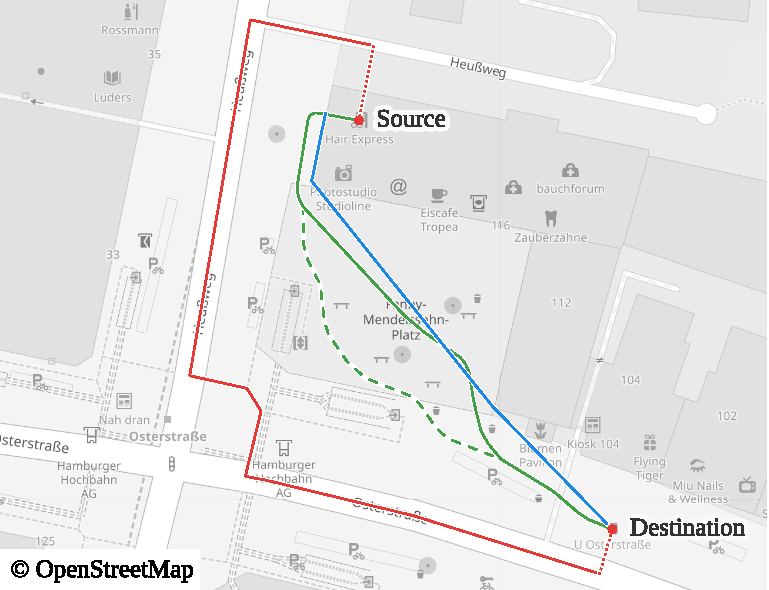
\includegraphics[width=\linewidth]{images/qgis-routing-osterstrasse}
				\end{figcenter}
				\caption[Comparison of normal routing with hybrid visibility routing.]{Graph-based route (red), hybrid routing algorithm result (blue) and the expected route (green). The dashed part of the expected result is an equally good alternative route.}
				\label{fig:eval-osterstrasse}
			\end{wrapfigure}
		
			In the following examples, routes determined by graph-based routing and the hybrid routing algorithm are compared against an expected result.
			This expected route was created based on OpenStreetMap data, aerial imagery and local knowledge.
			It was \emph{not} created to intentionally match the results from the hybrid routing algorithm.
		
			% From motivation
			The first situation, shown in \Cref{fig:eval-osterstrasse}, illustrates the problem of missing edges for graph-based algorithms.
			The square \enquote{Fanny-Mendelssohn Platz} in Hamburg, Germany, is a mostly unconnected area and therefore not traversable by graph-based algorithms.
			A routing request using GraphHopper\footnote{\url{https://www.osm.org/directions?engine=graphhopper\_foot\&route=53.57657,9.95210;53.57601,9.95268}} yields the red route, which does not cross the square due to missing edges and therefore takes a detour.
			The hybrid routing algorithm (blue path) does not entirely match the expected route but is a better approximation than the graph-based result.
			Next to this example, analyzing routes determined within the 1 km\textsuperscript{2} \enquote{OSM city} dataset yields some noteworthy findings.
			
			\begin{itemize}
				\item The route quality significantly decreases with missing or wrong data as shown in \Cref{fig:eval-osterstrasse} as well as \Cref{fig:eval-city-usefulness-b} to \ref{fig:eval-city-usefulness-c}.
				Red passages are not usable in the real world, often traversing private areas, which usually contain obstacles such as fences or vegetation.
				As described in \Cref{subsubsec:data-not-in-osm}, data of private areas in OSM is often sparse, resulting in these unrealistic routes.
				\item Within densely built-up areas, larger open spaces are rare and the combination of roads and buildings form corridors where routes tend to lie.
				When and how often a route determined by the hybrid routing algorithm follows a road depends on the weighting function.
				\item Larger roads result in wide obstacle-free corridor areas where unrealistic road crossings might appear.
				Such a situation can be seen in \Cref{fig:eval-city-road-crossing} with crossings over a six-lane road, which would be dangerous and unrealistic for real-world pedestrians.
				\item The weight function has a huge impact on the route quality.
				The weighting factors used in this work specify how strongly roads should be preferred, which is illustrated in \Cref{fig:eval-city-weights} with the same route using different weights for road edges.
				Adjusting and defining fine-grained weight functions may help to improve the route quality.
				\item In the \enquote{OSM city} datasets with only smaller open areas, graph-based routes and routes determined by the hybrid routing algorithm were often similar and some parts are even identical.
			\end{itemize}
			
			\begin{figure}[h!]
				\begin{minipage}[t]{.48\textwidth}
					\begin{subfigure}[t]{\linewidth}
						\begin{figcenter}
							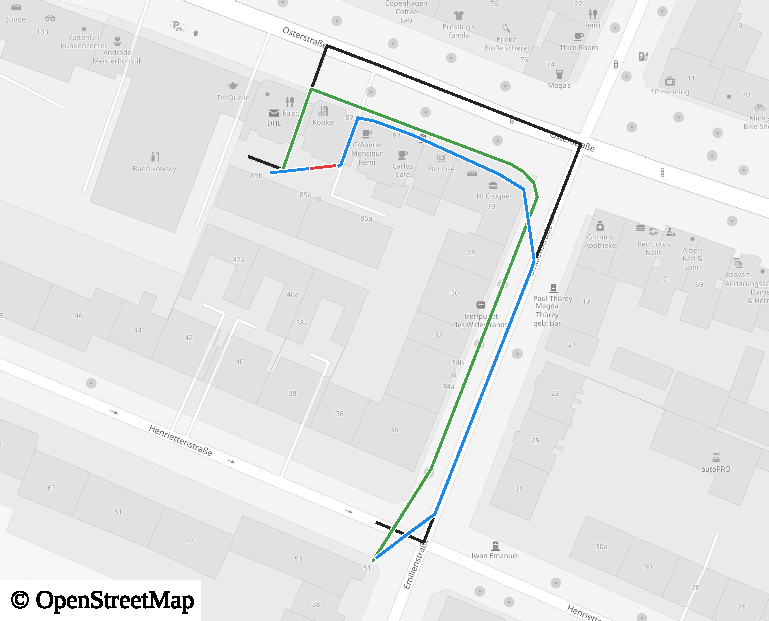
\includegraphics[width=\textwidth]{images/qgis-routing-city-routing-1}
						\end{figcenter}
						\caption{Simple route with only one small passage of missing data.}
						\label{fig:eval-city-usefulness-1}
					\end{subfigure}
				\end{minipage}
				\hfill
				\begin{minipage}[t]{.48\textwidth}
					\begin{subfigure}[t]{\linewidth}
						\begin{figcenter}
							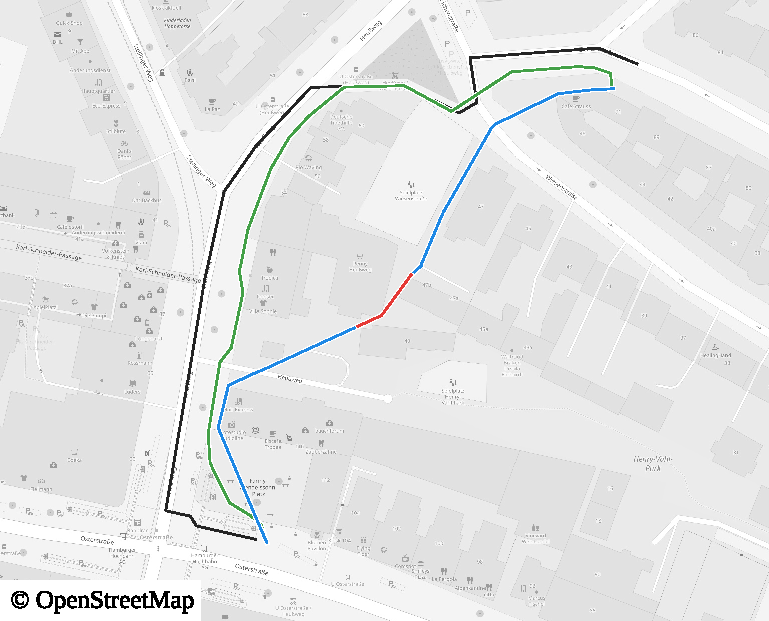
\includegraphics[width=\textwidth]{images/qgis-routing-city-routing-3}
						\end{figcenter}
						\caption{Missing obstacles (mainly walls and fences between buildings) lead to non-realistic routes.}
						\label{fig:eval-city-usefulness-b}
					\end{subfigure}
				\end{minipage}
				\\[3ex]
				\begin{minipage}[t]{.48\textwidth}
					\begin{subfigure}[t]{\linewidth}
						\begin{figcenter}
							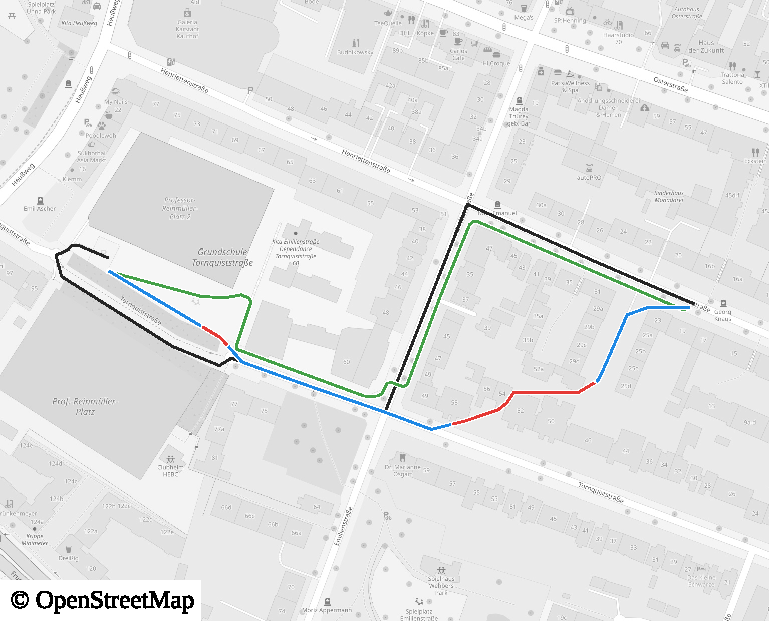
\includegraphics[width=\textwidth]{images/qgis-routing-city-routing-6}
						\end{figcenter}
						\caption{Missing walls, fences and hedges on private property are a common type of missing obstacles.}
						\label{fig:eval-city-usefulness-c}
					\end{subfigure}
				\end{minipage}
				\hfill
				\begin{minipage}[t]{.48\textwidth}
					\begin{subfigure}[t]{\linewidth}
						\begin{figcenter}
							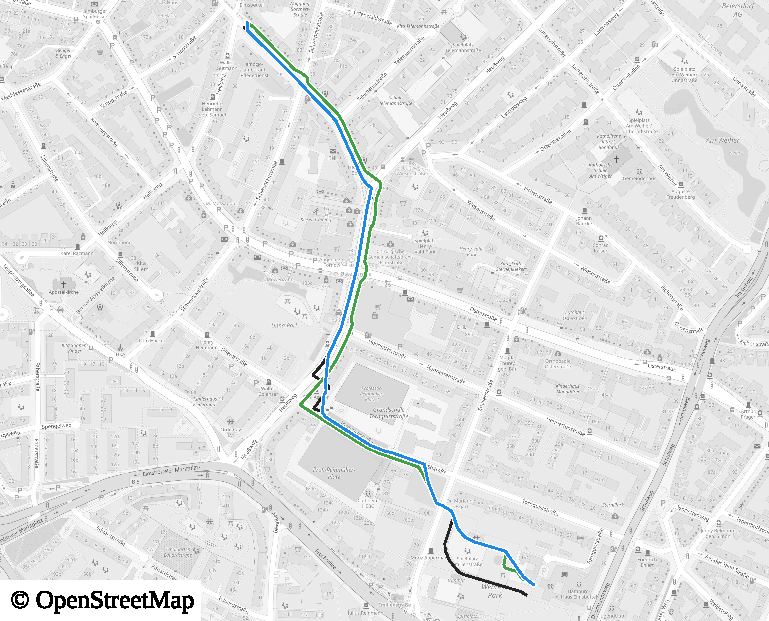
\includegraphics[width=\textwidth]{images/qgis-routing-city-routing-18}
						\end{figcenter}
						\caption{Cities with closed rows of buildings do not provide many degrees of freedom, resulting in similar or equal routes, regardless of the algorithm.}
						\label{fig:eval-city-usefulness-d}
					\end{subfigure}
				\end{minipage}
				\caption[Comparison of graph-based, actual and expected routes.]{Expected (green), graph-based (black) and hybrid routing algorithm results (blue) using the 1 km\textsuperscript{2} city dataset. Unexpected parts due to missing or faulty data are marked in red.}
				\label{fig:eval-city-usefulness}
			\end{figure}
			
			\begin{figure}[h!]
				\begin{minipage}[t]{.48\textwidth}
					\begin{figcenter}
						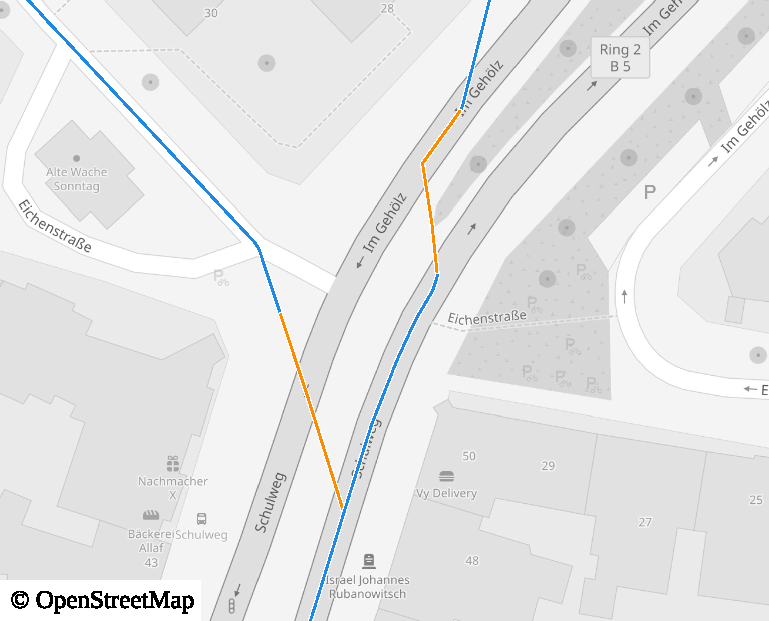
\includegraphics[width=\textwidth]{images/qgis-routing-city-roads}
					\end{figcenter}
					\caption{Two unrealistic road crossings (yellow) across a six-lane road.}
					\label{fig:eval-city-road-crossing}
				\end{minipage}
				\hfill
				\begin{minipage}[t]{.48\textwidth}
					\begin{figcenter}
						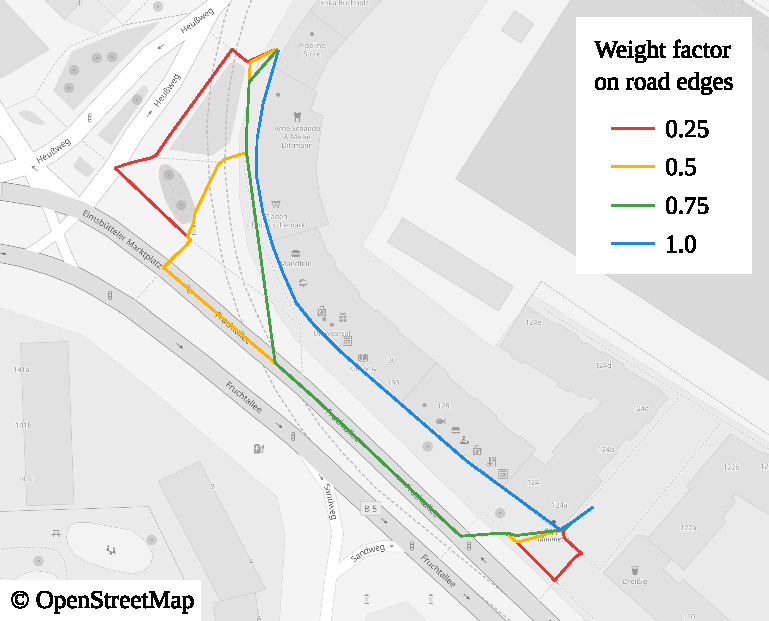
\includegraphics[width=\textwidth]{images/qgis-routing-city-weights}
					\end{figcenter}
					\caption{Influence of weight factors. Lower value result in a stronger preference for roads.}
					\label{fig:eval-city-weights}
				\end{minipage}
			\end{figure}
			
			% Interesting passages from the rural dataset
			\noindent
			Figures \Cref{fig:eval-rural-routing-6} and \ref{fig:eval-rural-graph-based-comparison} give examples of routes in a rural area with large open spaces.
			Two findings can be inferred from the analysis of the rural routing results.
			
			\begin{itemize}
				\item Datasets with larger open areas and irregularly distributed obstacles, as in the \enquote{OSM rural} datasets, can greatly benefit from the hybrid routing algorithm because graph-based routes might take long detours due to a sparse road network.
				\item The difference between graph-based routes and routes from the hybrid routing algorithm is significantly larger.
				They might not have any location in common and graph-based routes tend to be significantly longer.
				This can be seen in \Cref{fig:eval-rural-graph-based-comparison-6} with a 1.73 km long graph-based and 0.67 km long expected route.
				\Cref{fig:eval-rural-graph-based-comparison-17} shows a similar behavior even though the difference in distance is smaller because the graph-based, expected and actual route share common parts.
				\item The accuracy and therefore the usefulness for real-world applications (such as navigation apps) heavily depends on the level of detail in the dataset.
				\Cref{fig:eval-rural-routing-6-osm} illustrates the problem of missing data, in this case missing ditches within the farmland.
				The determined route has a length of 365 m, while the shortest possible route (determined using aerial imagery as seen in \Cref{fig:eval-rural-routing-6-aerial}) is 677 m long.
			\end{itemize}
			
			\begin{figure}[h!]
				\begin{minipage}[t]{.48\textwidth}
					\begin{subfigure}[t]{\linewidth}
						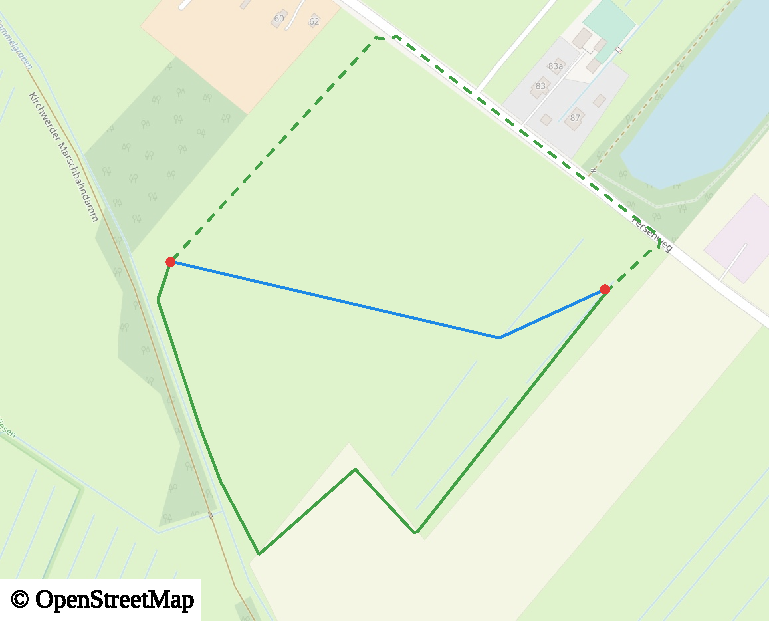
\includegraphics[width=\textwidth]{images/qgis-routing-rural-routing-6-osm}
						\caption{The expected route differs significantly from the actual route taken by the agent. The dashed line is an alternative route under the assumption that the farmland is reachable from the upper road.}
						\label{fig:eval-rural-routing-6-osm}
					\end{subfigure}
				\end{minipage}
				\hfill
				\begin{minipage}[t]{.48\textwidth}
					\begin{subfigure}[t]{\linewidth}
						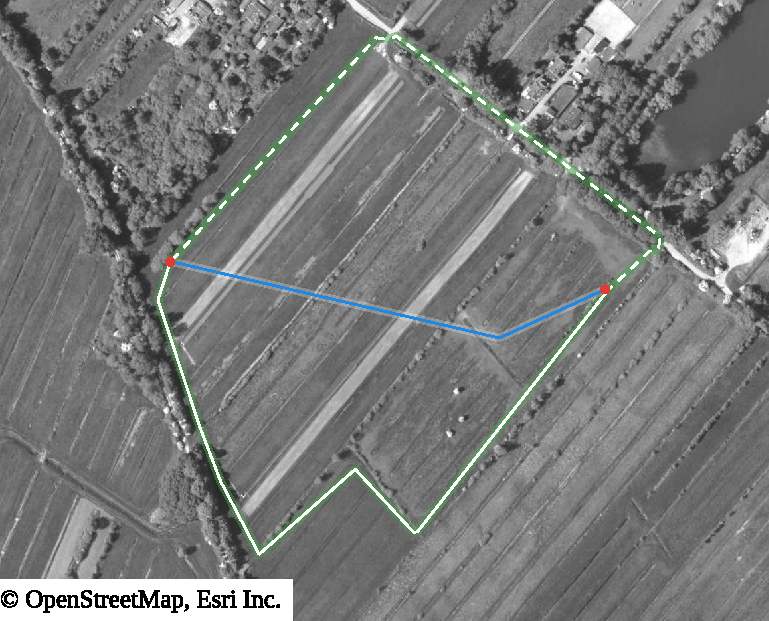
\includegraphics[width=\textwidth]{images/qgis-routing-rural-routing-6-aerial}
						\caption{Aerial imagery shows the amount of missing data, in this case numerous missing ditches within the farmland.}
						\label{fig:eval-rural-routing-6-aerial}
					\end{subfigure}
				\end{minipage}
				\caption[Illustration of routing problems and different weight-function values.]{Routing on farmland illustrating the importance of correct data in the routing result showing the expected route (green) and determined route by the hybrid routing algorithm (green).}
				\label{fig:eval-rural-routing-6}
			\end{figure}
			
			\begin{figure}[h!]
				\begin{minipage}[t]{.48\textwidth}
					\begin{subfigure}[t]{\linewidth}
						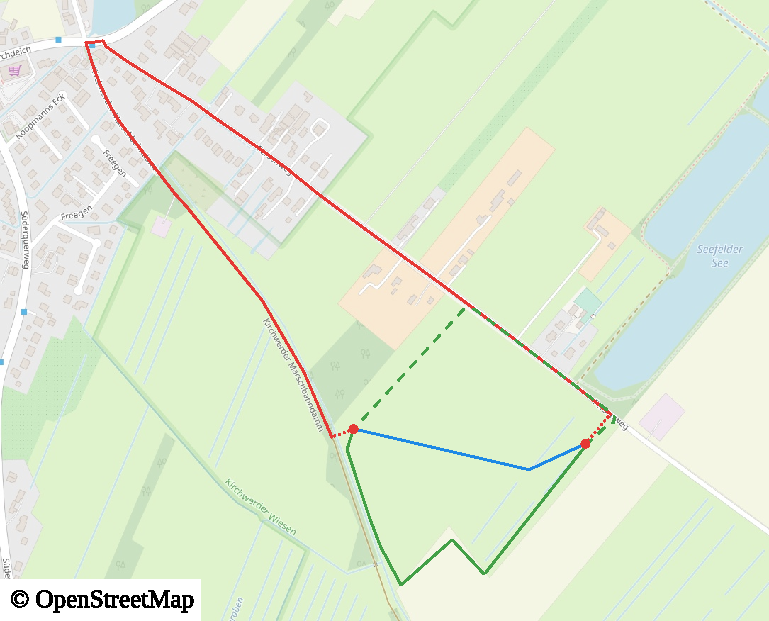
\includegraphics[width=\textwidth]{images/qgis-routing-rural-routing-6-graph-based}
						\caption{Same waypoints from \Cref{fig:eval-rural-routing-6} with the additional result of a graph-based routing request creating a 2.6 times longer path.}
						\label{fig:eval-rural-graph-based-comparison-6}
					\end{subfigure}
				\end{minipage}
				\hfill
				\begin{minipage}[t]{.48\textwidth}
					\begin{subfigure}[t]{\linewidth}
						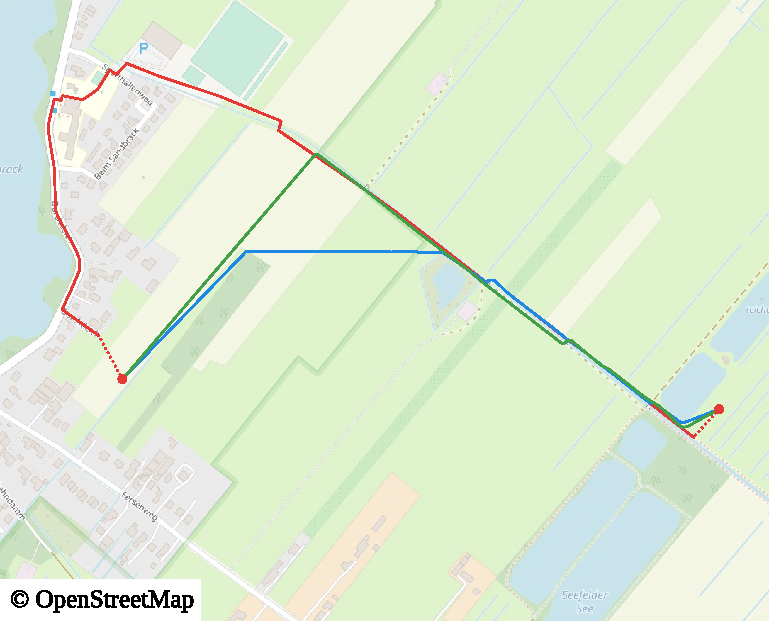
\includegraphics[width=\textwidth]{images/qgis-routing-rural-routing-17-graph-based}
						\caption{Detours created by a graph-based routing algorithm, even though the first part of the result is equal to the one of the hybrid routing algorithm. The shortcut of the actual result (horizontal part of the blue route) is a result of missing obstacles similar to the situation visible in \Cref{fig:eval-rural-routing-6-aerial}.}
						\label{fig:eval-rural-graph-based-comparison-17}
					\end{subfigure}
				\end{minipage}
				\caption[Visualization of the detour of graph-based routes.]{Comparison of graph-based routing results (red) with the expected route (green) and actual results (blue) of the hybrid routing algorithm.}
				\label{fig:eval-rural-graph-based-comparison}
			\end{figure}
			
			In general the manual route analysis showed that two main factors determine the route quality:
			the quality of the data (mainly determined by its completeness) and the weighting factor.
			The routes might still be good for densely built-up city datasets, even though a graph-based routing algorithm might yield similar routes.
		
		\subsubsection{Mathematical route quality analysis}
		
			Two mathematical approaches were used to obtain quantifiable results on the route quality.
			This was done by comparing the expected route to the graph-based and hybrid routing algorithm results.
			The first metric uses the beeline distance between two waypoints and compares it to the distances of the three corresponding routes.
			The second metric uses the Hausdorff distance (described below) to obtain a numeric similarity between the expected route and the two corresponding routing results.
			Both comparisons were performed on the first ten routing requests of the city and rural OSM datasets.
			
			\Cref{fig:eval-route-distances} shows the relation between the route and the beeline distances.
			The hybrid routing algorithm creates the shortest routes on average, which tend to be even shorter than the expected routes.
			Even though determining shortest routes is the overall goal, it indicates that missing obstacles lead to unrealistically short routes.
			This is in line with the results of the previous manual route analysis, according to which missing data leads to short but unrealistic routes.
			\begin{wrapfigure}{r}{0.35\textwidth}
%				\vspace{-0.55\baselineskip}
				\begin{figcenter}
					\begin{tikzpicture}
						[
						every node/.append style={outer sep=0.5mm, inner sep=0}
						]
						\def\d{0.75}
						
						\node (c00) at (0.6*\d ,0.1) {};
						\node (c01) at (1*\d   ,1*\d) {};
						\node (c02) at (0.15*\d ,2*\d) {};
						\node (c03) at (0.55*\d,3*\d) {};
						\node (c04) at (0      ,3.7*\d) {};
						
						\node (c10) at (1.8*\d  ,0.25) {};
						\node (c11) at (2.0*\d,0.9*\d) {};
						\node (c12) at (1.2*\d,1.8*\d) {};
						\node (c13) at (3*\d  ,2.8*\d) {};
						\node (c14) at (1.2*\d,3.8*\d) {};
						
						\draw (c00.center) -- (c01.center) -- (c02.center) -- (c03.center) -- (c04.center);
						\draw (c10.center) -- (c11.center) -- (c12.center) -- (c13.center) -- (c14.center);
						%						\draw (c01.center) -- (c02.center) -- (c03.center) -- (c04.center);
						%						\draw (c11.center) -- (c12.center) -- (c13.center) -- (c14.center);
						
						\draw[>=stealth',<->,densely dotted] (c00) -- (c10);
						\draw[>=stealth',<->,densely dotted] (c01) -- (c11);
						\draw[>=stealth',<->,densely dotted] (c02) -- (c12);
						\draw[>=stealth',<->,thick,red] (c03) -- (c13);
						\draw[>=stealth',<->,densely dotted] (c04) -- (c14);
						
						% Enlarge BBOX to avoid cropping off some of the arrow heads:
						\node (bbox_a) at (-0.05,0.05) {};
						\node (bbox_b) at (3*\d+0.05,3.8*\d+0.05) {};
					\end{tikzpicture}
				\end{figcenter}
				\caption[Illustration of the Hausdorff distance.]{Hausdorff distance (red) between two linestrings.}
				\label{fig:hausdorff-distance}
			\end{wrapfigure}
			The route length comparison also supports the previous results that graph-based routing leads to longer routes with sometimes significant detours, which can be seen in the routing requests 6 and 7 in \Cref{fig:eval-route-distances-rural}.
			Comparing routes by length only yields a vague indication of the route's quality.
			Therefore, the second metric uses the \term{Hausdorff distance} to quantify the similarity of two routes by determining the maximum distance between them as illustrated in \Cref{fig:hausdorff-distance}.
			\Cref{fig:eval-hausdorff} shows the results for both OSM datasets and yields some insights into the route similarities:
			\begin{itemize}
				\item In both datasets, the average Hausdorff distances of the routes determined using the hybrid routing algorithm are shorter than those of the graph-based algorithm.
				\item The difference is smaller in the city dataset, which supports the aforementioned hypothesis, that the buildings in a city create corridors leading to similar routes for graph-based and geometric routing algorithms.
				\item Except for the routing requests 6 and 7 in the \enquote{OSM rural} datasets, the Hausdorff distances of the routes by the hybrid routing algorithm tend to be larger than the distances of the graph-based routes.
				This is likely due to missing data, as discussed in the previous section and illustrated in \Cref{fig:eval-rural-routing-6}, leading to shorter but less realistic routes.
			\end{itemize}
			
			\begin{figure}[h!]
				\begin{subfigure}[t]{\linewidth}
					\begin{figcenter}
						%% Creator: Matplotlib, PGF backend
%%
%% To include the figure in your LaTeX document, write
%%   \input{<filename>.pgf}
%%
%% Make sure the required packages are loaded in your preamble
%%   \usepackage{pgf}
%%
%% Also ensure that all the required font packages are loaded; for instance,
%% the lmodern package is sometimes necessary when using math font.
%%   \usepackage{lmodern}
%%
%% Figures using additional raster images can only be included by \input if
%% they are in the same directory as the main LaTeX file. For loading figures
%% from other directories you can use the `import` package
%%   \usepackage{import}
%%
%% and then include the figures with
%%   \import{<path to file>}{<filename>.pgf}
%%
%% Matplotlib used the following preamble
%%   
%%   \usepackage{fontspec}
%%   \setmainfont{DejaVuSerif.ttf}[Path=\detokenize{/home/hauke/.local/lib/python3.11/site-packages/matplotlib/mpl-data/fonts/ttf/}]
%%   \setsansfont{DroidSans.ttf}[Path=\detokenize{/usr/share/fonts/droid/}]
%%   \setmonofont{DejaVuSansMono.ttf}[Path=\detokenize{/home/hauke/.local/lib/python3.11/site-packages/matplotlib/mpl-data/fonts/ttf/}]
%%   \makeatletter\@ifpackageloaded{underscore}{}{\usepackage[strings]{underscore}}\makeatother
%%
\begingroup%
\makeatletter%
\begin{pgfpicture}%
\pgfpathrectangle{\pgfpointorigin}{\pgfqpoint{6.086410in}{1.715788in}}%
\pgfusepath{use as bounding box, clip}%
\begin{pgfscope}%
\pgfsetbuttcap%
\pgfsetmiterjoin%
\definecolor{currentfill}{rgb}{1.000000,1.000000,1.000000}%
\pgfsetfillcolor{currentfill}%
\pgfsetlinewidth{0.000000pt}%
\definecolor{currentstroke}{rgb}{1.000000,1.000000,1.000000}%
\pgfsetstrokecolor{currentstroke}%
\pgfsetdash{}{0pt}%
\pgfpathmoveto{\pgfqpoint{0.000000in}{0.000000in}}%
\pgfpathlineto{\pgfqpoint{6.086410in}{0.000000in}}%
\pgfpathlineto{\pgfqpoint{6.086410in}{1.715788in}}%
\pgfpathlineto{\pgfqpoint{0.000000in}{1.715788in}}%
\pgfpathlineto{\pgfqpoint{0.000000in}{0.000000in}}%
\pgfpathclose%
\pgfusepath{fill}%
\end{pgfscope}%
\begin{pgfscope}%
\pgfsetbuttcap%
\pgfsetmiterjoin%
\definecolor{currentfill}{rgb}{1.000000,1.000000,1.000000}%
\pgfsetfillcolor{currentfill}%
\pgfsetlinewidth{0.000000pt}%
\definecolor{currentstroke}{rgb}{0.000000,0.000000,0.000000}%
\pgfsetstrokecolor{currentstroke}%
\pgfsetstrokeopacity{0.000000}%
\pgfsetdash{}{0pt}%
\pgfpathmoveto{\pgfqpoint{0.641586in}{0.451389in}}%
\pgfpathlineto{\pgfqpoint{4.921145in}{0.451389in}}%
\pgfpathlineto{\pgfqpoint{4.921145in}{1.715788in}}%
\pgfpathlineto{\pgfqpoint{0.641586in}{1.715788in}}%
\pgfpathlineto{\pgfqpoint{0.641586in}{0.451389in}}%
\pgfpathclose%
\pgfusepath{fill}%
\end{pgfscope}%
\begin{pgfscope}%
\definecolor{textcolor}{rgb}{0.150000,0.150000,0.150000}%
\pgfsetstrokecolor{textcolor}%
\pgfsetfillcolor{textcolor}%
\pgftext[x=0.836112in,y=0.319444in,,top]{\color{textcolor}\sffamily\fontsize{9.000000}{10.800000}\selectfont 1}%
\end{pgfscope}%
\begin{pgfscope}%
\definecolor{textcolor}{rgb}{0.150000,0.150000,0.150000}%
\pgfsetstrokecolor{textcolor}%
\pgfsetfillcolor{textcolor}%
\pgftext[x=1.225163in,y=0.319444in,,top]{\color{textcolor}\sffamily\fontsize{9.000000}{10.800000}\selectfont 2}%
\end{pgfscope}%
\begin{pgfscope}%
\definecolor{textcolor}{rgb}{0.150000,0.150000,0.150000}%
\pgfsetstrokecolor{textcolor}%
\pgfsetfillcolor{textcolor}%
\pgftext[x=1.614213in,y=0.319444in,,top]{\color{textcolor}\sffamily\fontsize{9.000000}{10.800000}\selectfont 3}%
\end{pgfscope}%
\begin{pgfscope}%
\definecolor{textcolor}{rgb}{0.150000,0.150000,0.150000}%
\pgfsetstrokecolor{textcolor}%
\pgfsetfillcolor{textcolor}%
\pgftext[x=2.003264in,y=0.319444in,,top]{\color{textcolor}\sffamily\fontsize{9.000000}{10.800000}\selectfont 4}%
\end{pgfscope}%
\begin{pgfscope}%
\definecolor{textcolor}{rgb}{0.150000,0.150000,0.150000}%
\pgfsetstrokecolor{textcolor}%
\pgfsetfillcolor{textcolor}%
\pgftext[x=2.392315in,y=0.319444in,,top]{\color{textcolor}\sffamily\fontsize{9.000000}{10.800000}\selectfont 5}%
\end{pgfscope}%
\begin{pgfscope}%
\definecolor{textcolor}{rgb}{0.150000,0.150000,0.150000}%
\pgfsetstrokecolor{textcolor}%
\pgfsetfillcolor{textcolor}%
\pgftext[x=2.781366in,y=0.319444in,,top]{\color{textcolor}\sffamily\fontsize{9.000000}{10.800000}\selectfont 6}%
\end{pgfscope}%
\begin{pgfscope}%
\definecolor{textcolor}{rgb}{0.150000,0.150000,0.150000}%
\pgfsetstrokecolor{textcolor}%
\pgfsetfillcolor{textcolor}%
\pgftext[x=3.170416in,y=0.319444in,,top]{\color{textcolor}\sffamily\fontsize{9.000000}{10.800000}\selectfont 7}%
\end{pgfscope}%
\begin{pgfscope}%
\definecolor{textcolor}{rgb}{0.150000,0.150000,0.150000}%
\pgfsetstrokecolor{textcolor}%
\pgfsetfillcolor{textcolor}%
\pgftext[x=3.559467in,y=0.319444in,,top]{\color{textcolor}\sffamily\fontsize{9.000000}{10.800000}\selectfont 8}%
\end{pgfscope}%
\begin{pgfscope}%
\definecolor{textcolor}{rgb}{0.150000,0.150000,0.150000}%
\pgfsetstrokecolor{textcolor}%
\pgfsetfillcolor{textcolor}%
\pgftext[x=3.948518in,y=0.319444in,,top]{\color{textcolor}\sffamily\fontsize{9.000000}{10.800000}\selectfont 9}%
\end{pgfscope}%
\begin{pgfscope}%
\definecolor{textcolor}{rgb}{0.150000,0.150000,0.150000}%
\pgfsetstrokecolor{textcolor}%
\pgfsetfillcolor{textcolor}%
\pgftext[x=4.337569in,y=0.319444in,,top]{\color{textcolor}\sffamily\fontsize{9.000000}{10.800000}\selectfont 10}%
\end{pgfscope}%
\begin{pgfscope}%
\definecolor{textcolor}{rgb}{0.150000,0.150000,0.150000}%
\pgfsetstrokecolor{textcolor}%
\pgfsetfillcolor{textcolor}%
\pgftext[x=4.726620in,y=0.319444in,,top]{\color{textcolor}\sffamily\fontsize{9.000000}{10.800000}\selectfont mean}%
\end{pgfscope}%
\begin{pgfscope}%
\definecolor{textcolor}{rgb}{0.150000,0.150000,0.150000}%
\pgfsetstrokecolor{textcolor}%
\pgfsetfillcolor{textcolor}%
\pgftext[x=2.781366in,y=0.125000in,,top]{\color{textcolor}\sffamily\fontsize{9.000000}{10.800000}\selectfont Routing request}%
\end{pgfscope}%
\begin{pgfscope}%
\pgfpathrectangle{\pgfqpoint{0.641586in}{0.451389in}}{\pgfqpoint{4.279559in}{1.264399in}}%
\pgfusepath{clip}%
\pgfsetroundcap%
\pgfsetroundjoin%
\pgfsetlinewidth{1.003750pt}%
\definecolor{currentstroke}{rgb}{0.800000,0.800000,0.800000}%
\pgfsetstrokecolor{currentstroke}%
\pgfsetdash{}{0pt}%
\pgfpathmoveto{\pgfqpoint{0.641586in}{0.537753in}}%
\pgfpathlineto{\pgfqpoint{4.921145in}{0.537753in}}%
\pgfusepath{stroke}%
\end{pgfscope}%
\begin{pgfscope}%
\definecolor{textcolor}{rgb}{0.150000,0.150000,0.150000}%
\pgfsetstrokecolor{textcolor}%
\pgfsetfillcolor{textcolor}%
\pgftext[x=0.338438in, y=0.490267in, left, base]{\color{textcolor}\sffamily\fontsize{9.000000}{10.800000}\selectfont 1.0}%
\end{pgfscope}%
\begin{pgfscope}%
\pgfpathrectangle{\pgfqpoint{0.641586in}{0.451389in}}{\pgfqpoint{4.279559in}{1.264399in}}%
\pgfusepath{clip}%
\pgfsetroundcap%
\pgfsetroundjoin%
\pgfsetlinewidth{1.003750pt}%
\definecolor{currentstroke}{rgb}{0.800000,0.800000,0.800000}%
\pgfsetstrokecolor{currentstroke}%
\pgfsetdash{}{0pt}%
\pgfpathmoveto{\pgfqpoint{0.641586in}{0.969573in}}%
\pgfpathlineto{\pgfqpoint{4.921145in}{0.969573in}}%
\pgfusepath{stroke}%
\end{pgfscope}%
\begin{pgfscope}%
\definecolor{textcolor}{rgb}{0.150000,0.150000,0.150000}%
\pgfsetstrokecolor{textcolor}%
\pgfsetfillcolor{textcolor}%
\pgftext[x=0.338438in, y=0.922088in, left, base]{\color{textcolor}\sffamily\fontsize{9.000000}{10.800000}\selectfont 1.5}%
\end{pgfscope}%
\begin{pgfscope}%
\pgfpathrectangle{\pgfqpoint{0.641586in}{0.451389in}}{\pgfqpoint{4.279559in}{1.264399in}}%
\pgfusepath{clip}%
\pgfsetroundcap%
\pgfsetroundjoin%
\pgfsetlinewidth{1.003750pt}%
\definecolor{currentstroke}{rgb}{0.800000,0.800000,0.800000}%
\pgfsetstrokecolor{currentstroke}%
\pgfsetdash{}{0pt}%
\pgfpathmoveto{\pgfqpoint{0.641586in}{1.401393in}}%
\pgfpathlineto{\pgfqpoint{4.921145in}{1.401393in}}%
\pgfusepath{stroke}%
\end{pgfscope}%
\begin{pgfscope}%
\definecolor{textcolor}{rgb}{0.150000,0.150000,0.150000}%
\pgfsetstrokecolor{textcolor}%
\pgfsetfillcolor{textcolor}%
\pgftext[x=0.338438in, y=1.353908in, left, base]{\color{textcolor}\sffamily\fontsize{9.000000}{10.800000}\selectfont 2.0}%
\end{pgfscope}%
\begin{pgfscope}%
\definecolor{textcolor}{rgb}{0.150000,0.150000,0.150000}%
\pgfsetstrokecolor{textcolor}%
\pgfsetfillcolor{textcolor}%
\pgftext[x=0.094971in, y=0.628907in, left, base,rotate=90.000000]{\color{textcolor}\sffamily\fontsize{9.000000}{10.800000}\selectfont Route distance /}%
\end{pgfscope}%
\begin{pgfscope}%
\definecolor{textcolor}{rgb}{0.150000,0.150000,0.150000}%
\pgfsetstrokecolor{textcolor}%
\pgfsetfillcolor{textcolor}%
\pgftext[x=0.238965in, y=0.626709in, left, base,rotate=90.000000]{\color{textcolor}\sffamily\fontsize{9.000000}{10.800000}\selectfont beeline distance}%
\end{pgfscope}%
\begin{pgfscope}%
\pgfpathrectangle{\pgfqpoint{0.641586in}{0.451389in}}{\pgfqpoint{4.279559in}{1.264399in}}%
\pgfusepath{clip}%
\pgfsetbuttcap%
\pgfsetmiterjoin%
\definecolor{currentfill}{rgb}{0.460784,0.749020,0.443137}%
\pgfsetfillcolor{currentfill}%
\pgfsetlinewidth{1.003750pt}%
\definecolor{currentstroke}{rgb}{1.000000,1.000000,1.000000}%
\pgfsetstrokecolor{currentstroke}%
\pgfsetdash{}{0pt}%
\pgfpathmoveto{\pgfqpoint{0.680491in}{-0.325888in}}%
\pgfpathlineto{\pgfqpoint{0.784238in}{-0.325888in}}%
\pgfpathlineto{\pgfqpoint{0.784238in}{1.307054in}}%
\pgfpathlineto{\pgfqpoint{0.680491in}{1.307054in}}%
\pgfpathlineto{\pgfqpoint{0.680491in}{-0.325888in}}%
\pgfpathclose%
\pgfusepath{stroke,fill}%
\end{pgfscope}%
\begin{pgfscope}%
\pgfpathrectangle{\pgfqpoint{0.641586in}{0.451389in}}{\pgfqpoint{4.279559in}{1.264399in}}%
\pgfusepath{clip}%
\pgfsetbuttcap%
\pgfsetmiterjoin%
\definecolor{currentfill}{rgb}{0.460784,0.749020,0.443137}%
\pgfsetfillcolor{currentfill}%
\pgfsetlinewidth{1.003750pt}%
\definecolor{currentstroke}{rgb}{1.000000,1.000000,1.000000}%
\pgfsetstrokecolor{currentstroke}%
\pgfsetdash{}{0pt}%
\pgfpathmoveto{\pgfqpoint{1.069542in}{-0.325888in}}%
\pgfpathlineto{\pgfqpoint{1.173289in}{-0.325888in}}%
\pgfpathlineto{\pgfqpoint{1.173289in}{0.742690in}}%
\pgfpathlineto{\pgfqpoint{1.069542in}{0.742690in}}%
\pgfpathlineto{\pgfqpoint{1.069542in}{-0.325888in}}%
\pgfpathclose%
\pgfusepath{stroke,fill}%
\end{pgfscope}%
\begin{pgfscope}%
\pgfpathrectangle{\pgfqpoint{0.641586in}{0.451389in}}{\pgfqpoint{4.279559in}{1.264399in}}%
\pgfusepath{clip}%
\pgfsetbuttcap%
\pgfsetmiterjoin%
\definecolor{currentfill}{rgb}{0.460784,0.749020,0.443137}%
\pgfsetfillcolor{currentfill}%
\pgfsetlinewidth{1.003750pt}%
\definecolor{currentstroke}{rgb}{1.000000,1.000000,1.000000}%
\pgfsetstrokecolor{currentstroke}%
\pgfsetdash{}{0pt}%
\pgfpathmoveto{\pgfqpoint{1.458593in}{-0.325888in}}%
\pgfpathlineto{\pgfqpoint{1.562340in}{-0.325888in}}%
\pgfpathlineto{\pgfqpoint{1.562340in}{0.919651in}}%
\pgfpathlineto{\pgfqpoint{1.458593in}{0.919651in}}%
\pgfpathlineto{\pgfqpoint{1.458593in}{-0.325888in}}%
\pgfpathclose%
\pgfusepath{stroke,fill}%
\end{pgfscope}%
\begin{pgfscope}%
\pgfpathrectangle{\pgfqpoint{0.641586in}{0.451389in}}{\pgfqpoint{4.279559in}{1.264399in}}%
\pgfusepath{clip}%
\pgfsetbuttcap%
\pgfsetmiterjoin%
\definecolor{currentfill}{rgb}{0.460784,0.749020,0.443137}%
\pgfsetfillcolor{currentfill}%
\pgfsetlinewidth{1.003750pt}%
\definecolor{currentstroke}{rgb}{1.000000,1.000000,1.000000}%
\pgfsetstrokecolor{currentstroke}%
\pgfsetdash{}{0pt}%
\pgfpathmoveto{\pgfqpoint{1.847644in}{-0.325888in}}%
\pgfpathlineto{\pgfqpoint{1.951391in}{-0.325888in}}%
\pgfpathlineto{\pgfqpoint{1.951391in}{0.553689in}}%
\pgfpathlineto{\pgfqpoint{1.847644in}{0.553689in}}%
\pgfpathlineto{\pgfqpoint{1.847644in}{-0.325888in}}%
\pgfpathclose%
\pgfusepath{stroke,fill}%
\end{pgfscope}%
\begin{pgfscope}%
\pgfpathrectangle{\pgfqpoint{0.641586in}{0.451389in}}{\pgfqpoint{4.279559in}{1.264399in}}%
\pgfusepath{clip}%
\pgfsetbuttcap%
\pgfsetmiterjoin%
\definecolor{currentfill}{rgb}{0.460784,0.749020,0.443137}%
\pgfsetfillcolor{currentfill}%
\pgfsetlinewidth{1.003750pt}%
\definecolor{currentstroke}{rgb}{1.000000,1.000000,1.000000}%
\pgfsetstrokecolor{currentstroke}%
\pgfsetdash{}{0pt}%
\pgfpathmoveto{\pgfqpoint{2.236695in}{-0.325888in}}%
\pgfpathlineto{\pgfqpoint{2.340441in}{-0.325888in}}%
\pgfpathlineto{\pgfqpoint{2.340441in}{1.254489in}}%
\pgfpathlineto{\pgfqpoint{2.236695in}{1.254489in}}%
\pgfpathlineto{\pgfqpoint{2.236695in}{-0.325888in}}%
\pgfpathclose%
\pgfusepath{stroke,fill}%
\end{pgfscope}%
\begin{pgfscope}%
\pgfpathrectangle{\pgfqpoint{0.641586in}{0.451389in}}{\pgfqpoint{4.279559in}{1.264399in}}%
\pgfusepath{clip}%
\pgfsetbuttcap%
\pgfsetmiterjoin%
\definecolor{currentfill}{rgb}{0.460784,0.749020,0.443137}%
\pgfsetfillcolor{currentfill}%
\pgfsetlinewidth{1.003750pt}%
\definecolor{currentstroke}{rgb}{1.000000,1.000000,1.000000}%
\pgfsetstrokecolor{currentstroke}%
\pgfsetdash{}{0pt}%
\pgfpathmoveto{\pgfqpoint{2.625745in}{-0.325888in}}%
\pgfpathlineto{\pgfqpoint{2.729492in}{-0.325888in}}%
\pgfpathlineto{\pgfqpoint{2.729492in}{0.860332in}}%
\pgfpathlineto{\pgfqpoint{2.625745in}{0.860332in}}%
\pgfpathlineto{\pgfqpoint{2.625745in}{-0.325888in}}%
\pgfpathclose%
\pgfusepath{stroke,fill}%
\end{pgfscope}%
\begin{pgfscope}%
\pgfpathrectangle{\pgfqpoint{0.641586in}{0.451389in}}{\pgfqpoint{4.279559in}{1.264399in}}%
\pgfusepath{clip}%
\pgfsetbuttcap%
\pgfsetmiterjoin%
\definecolor{currentfill}{rgb}{0.460784,0.749020,0.443137}%
\pgfsetfillcolor{currentfill}%
\pgfsetlinewidth{1.003750pt}%
\definecolor{currentstroke}{rgb}{1.000000,1.000000,1.000000}%
\pgfsetstrokecolor{currentstroke}%
\pgfsetdash{}{0pt}%
\pgfpathmoveto{\pgfqpoint{3.014796in}{-0.325888in}}%
\pgfpathlineto{\pgfqpoint{3.118543in}{-0.325888in}}%
\pgfpathlineto{\pgfqpoint{3.118543in}{0.930075in}}%
\pgfpathlineto{\pgfqpoint{3.014796in}{0.930075in}}%
\pgfpathlineto{\pgfqpoint{3.014796in}{-0.325888in}}%
\pgfpathclose%
\pgfusepath{stroke,fill}%
\end{pgfscope}%
\begin{pgfscope}%
\pgfpathrectangle{\pgfqpoint{0.641586in}{0.451389in}}{\pgfqpoint{4.279559in}{1.264399in}}%
\pgfusepath{clip}%
\pgfsetbuttcap%
\pgfsetmiterjoin%
\definecolor{currentfill}{rgb}{0.460784,0.749020,0.443137}%
\pgfsetfillcolor{currentfill}%
\pgfsetlinewidth{1.003750pt}%
\definecolor{currentstroke}{rgb}{1.000000,1.000000,1.000000}%
\pgfsetstrokecolor{currentstroke}%
\pgfsetdash{}{0pt}%
\pgfpathmoveto{\pgfqpoint{3.403847in}{-0.325888in}}%
\pgfpathlineto{\pgfqpoint{3.507594in}{-0.325888in}}%
\pgfpathlineto{\pgfqpoint{3.507594in}{1.025255in}}%
\pgfpathlineto{\pgfqpoint{3.403847in}{1.025255in}}%
\pgfpathlineto{\pgfqpoint{3.403847in}{-0.325888in}}%
\pgfpathclose%
\pgfusepath{stroke,fill}%
\end{pgfscope}%
\begin{pgfscope}%
\pgfpathrectangle{\pgfqpoint{0.641586in}{0.451389in}}{\pgfqpoint{4.279559in}{1.264399in}}%
\pgfusepath{clip}%
\pgfsetbuttcap%
\pgfsetmiterjoin%
\definecolor{currentfill}{rgb}{0.460784,0.749020,0.443137}%
\pgfsetfillcolor{currentfill}%
\pgfsetlinewidth{1.003750pt}%
\definecolor{currentstroke}{rgb}{1.000000,1.000000,1.000000}%
\pgfsetstrokecolor{currentstroke}%
\pgfsetdash{}{0pt}%
\pgfpathmoveto{\pgfqpoint{3.792898in}{-0.325888in}}%
\pgfpathlineto{\pgfqpoint{3.896645in}{-0.325888in}}%
\pgfpathlineto{\pgfqpoint{3.896645in}{0.923694in}}%
\pgfpathlineto{\pgfqpoint{3.792898in}{0.923694in}}%
\pgfpathlineto{\pgfqpoint{3.792898in}{-0.325888in}}%
\pgfpathclose%
\pgfusepath{stroke,fill}%
\end{pgfscope}%
\begin{pgfscope}%
\pgfpathrectangle{\pgfqpoint{0.641586in}{0.451389in}}{\pgfqpoint{4.279559in}{1.264399in}}%
\pgfusepath{clip}%
\pgfsetbuttcap%
\pgfsetmiterjoin%
\definecolor{currentfill}{rgb}{0.460784,0.749020,0.443137}%
\pgfsetfillcolor{currentfill}%
\pgfsetlinewidth{1.003750pt}%
\definecolor{currentstroke}{rgb}{1.000000,1.000000,1.000000}%
\pgfsetstrokecolor{currentstroke}%
\pgfsetdash{}{0pt}%
\pgfpathmoveto{\pgfqpoint{4.181948in}{-0.325888in}}%
\pgfpathlineto{\pgfqpoint{4.285695in}{-0.325888in}}%
\pgfpathlineto{\pgfqpoint{4.285695in}{1.087734in}}%
\pgfpathlineto{\pgfqpoint{4.181948in}{1.087734in}}%
\pgfpathlineto{\pgfqpoint{4.181948in}{-0.325888in}}%
\pgfpathclose%
\pgfusepath{stroke,fill}%
\end{pgfscope}%
\begin{pgfscope}%
\pgfpathrectangle{\pgfqpoint{0.641586in}{0.451389in}}{\pgfqpoint{4.279559in}{1.264399in}}%
\pgfusepath{clip}%
\pgfsetbuttcap%
\pgfsetmiterjoin%
\definecolor{currentfill}{rgb}{0.460784,0.749020,0.443137}%
\pgfsetfillcolor{currentfill}%
\pgfsetlinewidth{1.003750pt}%
\definecolor{currentstroke}{rgb}{1.000000,1.000000,1.000000}%
\pgfsetstrokecolor{currentstroke}%
\pgfsetdash{}{0pt}%
\pgfpathmoveto{\pgfqpoint{4.570999in}{-0.325888in}}%
\pgfpathlineto{\pgfqpoint{4.674746in}{-0.325888in}}%
\pgfpathlineto{\pgfqpoint{4.674746in}{0.960466in}}%
\pgfpathlineto{\pgfqpoint{4.570999in}{0.960466in}}%
\pgfpathlineto{\pgfqpoint{4.570999in}{-0.325888in}}%
\pgfpathclose%
\pgfusepath{stroke,fill}%
\end{pgfscope}%
\begin{pgfscope}%
\pgfpathrectangle{\pgfqpoint{0.641586in}{0.451389in}}{\pgfqpoint{4.279559in}{1.264399in}}%
\pgfusepath{clip}%
\pgfsetbuttcap%
\pgfsetmiterjoin%
\definecolor{currentfill}{rgb}{0.349020,0.490196,0.749020}%
\pgfsetfillcolor{currentfill}%
\pgfsetlinewidth{1.003750pt}%
\definecolor{currentstroke}{rgb}{1.000000,1.000000,1.000000}%
\pgfsetstrokecolor{currentstroke}%
\pgfsetdash{}{0pt}%
\pgfpathmoveto{\pgfqpoint{0.784238in}{-0.325888in}}%
\pgfpathlineto{\pgfqpoint{0.887985in}{-0.325888in}}%
\pgfpathlineto{\pgfqpoint{0.887985in}{1.271194in}}%
\pgfpathlineto{\pgfqpoint{0.784238in}{1.271194in}}%
\pgfpathlineto{\pgfqpoint{0.784238in}{-0.325888in}}%
\pgfpathclose%
\pgfusepath{stroke,fill}%
\end{pgfscope}%
\begin{pgfscope}%
\pgfpathrectangle{\pgfqpoint{0.641586in}{0.451389in}}{\pgfqpoint{4.279559in}{1.264399in}}%
\pgfusepath{clip}%
\pgfsetbuttcap%
\pgfsetmiterjoin%
\definecolor{currentfill}{rgb}{0.349020,0.490196,0.749020}%
\pgfsetfillcolor{currentfill}%
\pgfsetlinewidth{1.003750pt}%
\definecolor{currentstroke}{rgb}{1.000000,1.000000,1.000000}%
\pgfsetstrokecolor{currentstroke}%
\pgfsetdash{}{0pt}%
\pgfpathmoveto{\pgfqpoint{1.173289in}{-0.325888in}}%
\pgfpathlineto{\pgfqpoint{1.277036in}{-0.325888in}}%
\pgfpathlineto{\pgfqpoint{1.277036in}{0.682497in}}%
\pgfpathlineto{\pgfqpoint{1.173289in}{0.682497in}}%
\pgfpathlineto{\pgfqpoint{1.173289in}{-0.325888in}}%
\pgfpathclose%
\pgfusepath{stroke,fill}%
\end{pgfscope}%
\begin{pgfscope}%
\pgfpathrectangle{\pgfqpoint{0.641586in}{0.451389in}}{\pgfqpoint{4.279559in}{1.264399in}}%
\pgfusepath{clip}%
\pgfsetbuttcap%
\pgfsetmiterjoin%
\definecolor{currentfill}{rgb}{0.349020,0.490196,0.749020}%
\pgfsetfillcolor{currentfill}%
\pgfsetlinewidth{1.003750pt}%
\definecolor{currentstroke}{rgb}{1.000000,1.000000,1.000000}%
\pgfsetstrokecolor{currentstroke}%
\pgfsetdash{}{0pt}%
\pgfpathmoveto{\pgfqpoint{1.562340in}{-0.325888in}}%
\pgfpathlineto{\pgfqpoint{1.666087in}{-0.325888in}}%
\pgfpathlineto{\pgfqpoint{1.666087in}{0.722822in}}%
\pgfpathlineto{\pgfqpoint{1.562340in}{0.722822in}}%
\pgfpathlineto{\pgfqpoint{1.562340in}{-0.325888in}}%
\pgfpathclose%
\pgfusepath{stroke,fill}%
\end{pgfscope}%
\begin{pgfscope}%
\pgfpathrectangle{\pgfqpoint{0.641586in}{0.451389in}}{\pgfqpoint{4.279559in}{1.264399in}}%
\pgfusepath{clip}%
\pgfsetbuttcap%
\pgfsetmiterjoin%
\definecolor{currentfill}{rgb}{0.349020,0.490196,0.749020}%
\pgfsetfillcolor{currentfill}%
\pgfsetlinewidth{1.003750pt}%
\definecolor{currentstroke}{rgb}{1.000000,1.000000,1.000000}%
\pgfsetstrokecolor{currentstroke}%
\pgfsetdash{}{0pt}%
\pgfpathmoveto{\pgfqpoint{1.951391in}{-0.325888in}}%
\pgfpathlineto{\pgfqpoint{2.055138in}{-0.325888in}}%
\pgfpathlineto{\pgfqpoint{2.055138in}{0.560543in}}%
\pgfpathlineto{\pgfqpoint{1.951391in}{0.560543in}}%
\pgfpathlineto{\pgfqpoint{1.951391in}{-0.325888in}}%
\pgfpathclose%
\pgfusepath{stroke,fill}%
\end{pgfscope}%
\begin{pgfscope}%
\pgfpathrectangle{\pgfqpoint{0.641586in}{0.451389in}}{\pgfqpoint{4.279559in}{1.264399in}}%
\pgfusepath{clip}%
\pgfsetbuttcap%
\pgfsetmiterjoin%
\definecolor{currentfill}{rgb}{0.349020,0.490196,0.749020}%
\pgfsetfillcolor{currentfill}%
\pgfsetlinewidth{1.003750pt}%
\definecolor{currentstroke}{rgb}{1.000000,1.000000,1.000000}%
\pgfsetstrokecolor{currentstroke}%
\pgfsetdash{}{0pt}%
\pgfpathmoveto{\pgfqpoint{2.340441in}{-0.325888in}}%
\pgfpathlineto{\pgfqpoint{2.444188in}{-0.325888in}}%
\pgfpathlineto{\pgfqpoint{2.444188in}{0.634284in}}%
\pgfpathlineto{\pgfqpoint{2.340441in}{0.634284in}}%
\pgfpathlineto{\pgfqpoint{2.340441in}{-0.325888in}}%
\pgfpathclose%
\pgfusepath{stroke,fill}%
\end{pgfscope}%
\begin{pgfscope}%
\pgfpathrectangle{\pgfqpoint{0.641586in}{0.451389in}}{\pgfqpoint{4.279559in}{1.264399in}}%
\pgfusepath{clip}%
\pgfsetbuttcap%
\pgfsetmiterjoin%
\definecolor{currentfill}{rgb}{0.349020,0.490196,0.749020}%
\pgfsetfillcolor{currentfill}%
\pgfsetlinewidth{1.003750pt}%
\definecolor{currentstroke}{rgb}{1.000000,1.000000,1.000000}%
\pgfsetstrokecolor{currentstroke}%
\pgfsetdash{}{0pt}%
\pgfpathmoveto{\pgfqpoint{2.729492in}{-0.325888in}}%
\pgfpathlineto{\pgfqpoint{2.833239in}{-0.325888in}}%
\pgfpathlineto{\pgfqpoint{2.833239in}{0.678706in}}%
\pgfpathlineto{\pgfqpoint{2.729492in}{0.678706in}}%
\pgfpathlineto{\pgfqpoint{2.729492in}{-0.325888in}}%
\pgfpathclose%
\pgfusepath{stroke,fill}%
\end{pgfscope}%
\begin{pgfscope}%
\pgfpathrectangle{\pgfqpoint{0.641586in}{0.451389in}}{\pgfqpoint{4.279559in}{1.264399in}}%
\pgfusepath{clip}%
\pgfsetbuttcap%
\pgfsetmiterjoin%
\definecolor{currentfill}{rgb}{0.349020,0.490196,0.749020}%
\pgfsetfillcolor{currentfill}%
\pgfsetlinewidth{1.003750pt}%
\definecolor{currentstroke}{rgb}{1.000000,1.000000,1.000000}%
\pgfsetstrokecolor{currentstroke}%
\pgfsetdash{}{0pt}%
\pgfpathmoveto{\pgfqpoint{3.118543in}{-0.325888in}}%
\pgfpathlineto{\pgfqpoint{3.222290in}{-0.325888in}}%
\pgfpathlineto{\pgfqpoint{3.222290in}{0.859033in}}%
\pgfpathlineto{\pgfqpoint{3.118543in}{0.859033in}}%
\pgfpathlineto{\pgfqpoint{3.118543in}{-0.325888in}}%
\pgfpathclose%
\pgfusepath{stroke,fill}%
\end{pgfscope}%
\begin{pgfscope}%
\pgfpathrectangle{\pgfqpoint{0.641586in}{0.451389in}}{\pgfqpoint{4.279559in}{1.264399in}}%
\pgfusepath{clip}%
\pgfsetbuttcap%
\pgfsetmiterjoin%
\definecolor{currentfill}{rgb}{0.349020,0.490196,0.749020}%
\pgfsetfillcolor{currentfill}%
\pgfsetlinewidth{1.003750pt}%
\definecolor{currentstroke}{rgb}{1.000000,1.000000,1.000000}%
\pgfsetstrokecolor{currentstroke}%
\pgfsetdash{}{0pt}%
\pgfpathmoveto{\pgfqpoint{3.507594in}{-0.325888in}}%
\pgfpathlineto{\pgfqpoint{3.611341in}{-0.325888in}}%
\pgfpathlineto{\pgfqpoint{3.611341in}{0.845438in}}%
\pgfpathlineto{\pgfqpoint{3.507594in}{0.845438in}}%
\pgfpathlineto{\pgfqpoint{3.507594in}{-0.325888in}}%
\pgfpathclose%
\pgfusepath{stroke,fill}%
\end{pgfscope}%
\begin{pgfscope}%
\pgfpathrectangle{\pgfqpoint{0.641586in}{0.451389in}}{\pgfqpoint{4.279559in}{1.264399in}}%
\pgfusepath{clip}%
\pgfsetbuttcap%
\pgfsetmiterjoin%
\definecolor{currentfill}{rgb}{0.349020,0.490196,0.749020}%
\pgfsetfillcolor{currentfill}%
\pgfsetlinewidth{1.003750pt}%
\definecolor{currentstroke}{rgb}{1.000000,1.000000,1.000000}%
\pgfsetstrokecolor{currentstroke}%
\pgfsetdash{}{0pt}%
\pgfpathmoveto{\pgfqpoint{3.896645in}{-0.325888in}}%
\pgfpathlineto{\pgfqpoint{4.000391in}{-0.325888in}}%
\pgfpathlineto{\pgfqpoint{4.000391in}{0.770601in}}%
\pgfpathlineto{\pgfqpoint{3.896645in}{0.770601in}}%
\pgfpathlineto{\pgfqpoint{3.896645in}{-0.325888in}}%
\pgfpathclose%
\pgfusepath{stroke,fill}%
\end{pgfscope}%
\begin{pgfscope}%
\pgfpathrectangle{\pgfqpoint{0.641586in}{0.451389in}}{\pgfqpoint{4.279559in}{1.264399in}}%
\pgfusepath{clip}%
\pgfsetbuttcap%
\pgfsetmiterjoin%
\definecolor{currentfill}{rgb}{0.349020,0.490196,0.749020}%
\pgfsetfillcolor{currentfill}%
\pgfsetlinewidth{1.003750pt}%
\definecolor{currentstroke}{rgb}{1.000000,1.000000,1.000000}%
\pgfsetstrokecolor{currentstroke}%
\pgfsetdash{}{0pt}%
\pgfpathmoveto{\pgfqpoint{4.285695in}{-0.325888in}}%
\pgfpathlineto{\pgfqpoint{4.389442in}{-0.325888in}}%
\pgfpathlineto{\pgfqpoint{4.389442in}{0.892496in}}%
\pgfpathlineto{\pgfqpoint{4.285695in}{0.892496in}}%
\pgfpathlineto{\pgfqpoint{4.285695in}{-0.325888in}}%
\pgfpathclose%
\pgfusepath{stroke,fill}%
\end{pgfscope}%
\begin{pgfscope}%
\pgfpathrectangle{\pgfqpoint{0.641586in}{0.451389in}}{\pgfqpoint{4.279559in}{1.264399in}}%
\pgfusepath{clip}%
\pgfsetbuttcap%
\pgfsetmiterjoin%
\definecolor{currentfill}{rgb}{0.349020,0.490196,0.749020}%
\pgfsetfillcolor{currentfill}%
\pgfsetlinewidth{1.003750pt}%
\definecolor{currentstroke}{rgb}{1.000000,1.000000,1.000000}%
\pgfsetstrokecolor{currentstroke}%
\pgfsetdash{}{0pt}%
\pgfpathmoveto{\pgfqpoint{4.674746in}{-0.325888in}}%
\pgfpathlineto{\pgfqpoint{4.778493in}{-0.325888in}}%
\pgfpathlineto{\pgfqpoint{4.778493in}{0.791761in}}%
\pgfpathlineto{\pgfqpoint{4.674746in}{0.791761in}}%
\pgfpathlineto{\pgfqpoint{4.674746in}{-0.325888in}}%
\pgfpathclose%
\pgfusepath{stroke,fill}%
\end{pgfscope}%
\begin{pgfscope}%
\pgfpathrectangle{\pgfqpoint{0.641586in}{0.451389in}}{\pgfqpoint{4.279559in}{1.264399in}}%
\pgfusepath{clip}%
\pgfsetbuttcap%
\pgfsetmiterjoin%
\definecolor{currentfill}{rgb}{0.852941,0.544118,0.370588}%
\pgfsetfillcolor{currentfill}%
\pgfsetlinewidth{1.003750pt}%
\definecolor{currentstroke}{rgb}{1.000000,1.000000,1.000000}%
\pgfsetstrokecolor{currentstroke}%
\pgfsetdash{}{0pt}%
\pgfpathmoveto{\pgfqpoint{0.887985in}{-0.325888in}}%
\pgfpathlineto{\pgfqpoint{0.991732in}{-0.325888in}}%
\pgfpathlineto{\pgfqpoint{0.991732in}{1.618565in}}%
\pgfpathlineto{\pgfqpoint{0.887985in}{1.618565in}}%
\pgfpathlineto{\pgfqpoint{0.887985in}{-0.325888in}}%
\pgfpathclose%
\pgfusepath{stroke,fill}%
\end{pgfscope}%
\begin{pgfscope}%
\pgfpathrectangle{\pgfqpoint{0.641586in}{0.451389in}}{\pgfqpoint{4.279559in}{1.264399in}}%
\pgfusepath{clip}%
\pgfsetbuttcap%
\pgfsetmiterjoin%
\definecolor{currentfill}{rgb}{0.852941,0.544118,0.370588}%
\pgfsetfillcolor{currentfill}%
\pgfsetlinewidth{1.003750pt}%
\definecolor{currentstroke}{rgb}{1.000000,1.000000,1.000000}%
\pgfsetstrokecolor{currentstroke}%
\pgfsetdash{}{0pt}%
\pgfpathmoveto{\pgfqpoint{1.277036in}{-0.325888in}}%
\pgfpathlineto{\pgfqpoint{1.380783in}{-0.325888in}}%
\pgfpathlineto{\pgfqpoint{1.380783in}{1.068830in}}%
\pgfpathlineto{\pgfqpoint{1.277036in}{1.068830in}}%
\pgfpathlineto{\pgfqpoint{1.277036in}{-0.325888in}}%
\pgfpathclose%
\pgfusepath{stroke,fill}%
\end{pgfscope}%
\begin{pgfscope}%
\pgfpathrectangle{\pgfqpoint{0.641586in}{0.451389in}}{\pgfqpoint{4.279559in}{1.264399in}}%
\pgfusepath{clip}%
\pgfsetbuttcap%
\pgfsetmiterjoin%
\definecolor{currentfill}{rgb}{0.852941,0.544118,0.370588}%
\pgfsetfillcolor{currentfill}%
\pgfsetlinewidth{1.003750pt}%
\definecolor{currentstroke}{rgb}{1.000000,1.000000,1.000000}%
\pgfsetstrokecolor{currentstroke}%
\pgfsetdash{}{0pt}%
\pgfpathmoveto{\pgfqpoint{1.666087in}{-0.325888in}}%
\pgfpathlineto{\pgfqpoint{1.769834in}{-0.325888in}}%
\pgfpathlineto{\pgfqpoint{1.769834in}{1.161862in}}%
\pgfpathlineto{\pgfqpoint{1.666087in}{1.161862in}}%
\pgfpathlineto{\pgfqpoint{1.666087in}{-0.325888in}}%
\pgfpathclose%
\pgfusepath{stroke,fill}%
\end{pgfscope}%
\begin{pgfscope}%
\pgfpathrectangle{\pgfqpoint{0.641586in}{0.451389in}}{\pgfqpoint{4.279559in}{1.264399in}}%
\pgfusepath{clip}%
\pgfsetbuttcap%
\pgfsetmiterjoin%
\definecolor{currentfill}{rgb}{0.852941,0.544118,0.370588}%
\pgfsetfillcolor{currentfill}%
\pgfsetlinewidth{1.003750pt}%
\definecolor{currentstroke}{rgb}{1.000000,1.000000,1.000000}%
\pgfsetstrokecolor{currentstroke}%
\pgfsetdash{}{0pt}%
\pgfpathmoveto{\pgfqpoint{2.055138in}{-0.325888in}}%
\pgfpathlineto{\pgfqpoint{2.158884in}{-0.325888in}}%
\pgfpathlineto{\pgfqpoint{2.158884in}{0.598130in}}%
\pgfpathlineto{\pgfqpoint{2.055138in}{0.598130in}}%
\pgfpathlineto{\pgfqpoint{2.055138in}{-0.325888in}}%
\pgfpathclose%
\pgfusepath{stroke,fill}%
\end{pgfscope}%
\begin{pgfscope}%
\pgfpathrectangle{\pgfqpoint{0.641586in}{0.451389in}}{\pgfqpoint{4.279559in}{1.264399in}}%
\pgfusepath{clip}%
\pgfsetbuttcap%
\pgfsetmiterjoin%
\definecolor{currentfill}{rgb}{0.852941,0.544118,0.370588}%
\pgfsetfillcolor{currentfill}%
\pgfsetlinewidth{1.003750pt}%
\definecolor{currentstroke}{rgb}{1.000000,1.000000,1.000000}%
\pgfsetstrokecolor{currentstroke}%
\pgfsetdash{}{0pt}%
\pgfpathmoveto{\pgfqpoint{2.444188in}{-0.325888in}}%
\pgfpathlineto{\pgfqpoint{2.547935in}{-0.325888in}}%
\pgfpathlineto{\pgfqpoint{2.547935in}{1.199276in}}%
\pgfpathlineto{\pgfqpoint{2.444188in}{1.199276in}}%
\pgfpathlineto{\pgfqpoint{2.444188in}{-0.325888in}}%
\pgfpathclose%
\pgfusepath{stroke,fill}%
\end{pgfscope}%
\begin{pgfscope}%
\pgfpathrectangle{\pgfqpoint{0.641586in}{0.451389in}}{\pgfqpoint{4.279559in}{1.264399in}}%
\pgfusepath{clip}%
\pgfsetbuttcap%
\pgfsetmiterjoin%
\definecolor{currentfill}{rgb}{0.852941,0.544118,0.370588}%
\pgfsetfillcolor{currentfill}%
\pgfsetlinewidth{1.003750pt}%
\definecolor{currentstroke}{rgb}{1.000000,1.000000,1.000000}%
\pgfsetstrokecolor{currentstroke}%
\pgfsetdash{}{0pt}%
\pgfpathmoveto{\pgfqpoint{2.833239in}{-0.325888in}}%
\pgfpathlineto{\pgfqpoint{2.936986in}{-0.325888in}}%
\pgfpathlineto{\pgfqpoint{2.936986in}{1.050470in}}%
\pgfpathlineto{\pgfqpoint{2.833239in}{1.050470in}}%
\pgfpathlineto{\pgfqpoint{2.833239in}{-0.325888in}}%
\pgfpathclose%
\pgfusepath{stroke,fill}%
\end{pgfscope}%
\begin{pgfscope}%
\pgfpathrectangle{\pgfqpoint{0.641586in}{0.451389in}}{\pgfqpoint{4.279559in}{1.264399in}}%
\pgfusepath{clip}%
\pgfsetbuttcap%
\pgfsetmiterjoin%
\definecolor{currentfill}{rgb}{0.852941,0.544118,0.370588}%
\pgfsetfillcolor{currentfill}%
\pgfsetlinewidth{1.003750pt}%
\definecolor{currentstroke}{rgb}{1.000000,1.000000,1.000000}%
\pgfsetstrokecolor{currentstroke}%
\pgfsetdash{}{0pt}%
\pgfpathmoveto{\pgfqpoint{3.222290in}{-0.325888in}}%
\pgfpathlineto{\pgfqpoint{3.326037in}{-0.325888in}}%
\pgfpathlineto{\pgfqpoint{3.326037in}{1.088948in}}%
\pgfpathlineto{\pgfqpoint{3.222290in}{1.088948in}}%
\pgfpathlineto{\pgfqpoint{3.222290in}{-0.325888in}}%
\pgfpathclose%
\pgfusepath{stroke,fill}%
\end{pgfscope}%
\begin{pgfscope}%
\pgfpathrectangle{\pgfqpoint{0.641586in}{0.451389in}}{\pgfqpoint{4.279559in}{1.264399in}}%
\pgfusepath{clip}%
\pgfsetbuttcap%
\pgfsetmiterjoin%
\definecolor{currentfill}{rgb}{0.852941,0.544118,0.370588}%
\pgfsetfillcolor{currentfill}%
\pgfsetlinewidth{1.003750pt}%
\definecolor{currentstroke}{rgb}{1.000000,1.000000,1.000000}%
\pgfsetstrokecolor{currentstroke}%
\pgfsetdash{}{0pt}%
\pgfpathmoveto{\pgfqpoint{3.611341in}{-0.325888in}}%
\pgfpathlineto{\pgfqpoint{3.715087in}{-0.325888in}}%
\pgfpathlineto{\pgfqpoint{3.715087in}{1.142096in}}%
\pgfpathlineto{\pgfqpoint{3.611341in}{1.142096in}}%
\pgfpathlineto{\pgfqpoint{3.611341in}{-0.325888in}}%
\pgfpathclose%
\pgfusepath{stroke,fill}%
\end{pgfscope}%
\begin{pgfscope}%
\pgfpathrectangle{\pgfqpoint{0.641586in}{0.451389in}}{\pgfqpoint{4.279559in}{1.264399in}}%
\pgfusepath{clip}%
\pgfsetbuttcap%
\pgfsetmiterjoin%
\definecolor{currentfill}{rgb}{0.852941,0.544118,0.370588}%
\pgfsetfillcolor{currentfill}%
\pgfsetlinewidth{1.003750pt}%
\definecolor{currentstroke}{rgb}{1.000000,1.000000,1.000000}%
\pgfsetstrokecolor{currentstroke}%
\pgfsetdash{}{0pt}%
\pgfpathmoveto{\pgfqpoint{4.000391in}{-0.325888in}}%
\pgfpathlineto{\pgfqpoint{4.104138in}{-0.325888in}}%
\pgfpathlineto{\pgfqpoint{4.104138in}{1.009572in}}%
\pgfpathlineto{\pgfqpoint{4.000391in}{1.009572in}}%
\pgfpathlineto{\pgfqpoint{4.000391in}{-0.325888in}}%
\pgfpathclose%
\pgfusepath{stroke,fill}%
\end{pgfscope}%
\begin{pgfscope}%
\pgfpathrectangle{\pgfqpoint{0.641586in}{0.451389in}}{\pgfqpoint{4.279559in}{1.264399in}}%
\pgfusepath{clip}%
\pgfsetbuttcap%
\pgfsetmiterjoin%
\definecolor{currentfill}{rgb}{0.852941,0.544118,0.370588}%
\pgfsetfillcolor{currentfill}%
\pgfsetlinewidth{1.003750pt}%
\definecolor{currentstroke}{rgb}{1.000000,1.000000,1.000000}%
\pgfsetstrokecolor{currentstroke}%
\pgfsetdash{}{0pt}%
\pgfpathmoveto{\pgfqpoint{4.389442in}{-0.325888in}}%
\pgfpathlineto{\pgfqpoint{4.493189in}{-0.325888in}}%
\pgfpathlineto{\pgfqpoint{4.493189in}{1.128945in}}%
\pgfpathlineto{\pgfqpoint{4.389442in}{1.128945in}}%
\pgfpathlineto{\pgfqpoint{4.389442in}{-0.325888in}}%
\pgfpathclose%
\pgfusepath{stroke,fill}%
\end{pgfscope}%
\begin{pgfscope}%
\pgfpathrectangle{\pgfqpoint{0.641586in}{0.451389in}}{\pgfqpoint{4.279559in}{1.264399in}}%
\pgfusepath{clip}%
\pgfsetbuttcap%
\pgfsetmiterjoin%
\definecolor{currentfill}{rgb}{0.852941,0.544118,0.370588}%
\pgfsetfillcolor{currentfill}%
\pgfsetlinewidth{1.003750pt}%
\definecolor{currentstroke}{rgb}{1.000000,1.000000,1.000000}%
\pgfsetstrokecolor{currentstroke}%
\pgfsetdash{}{0pt}%
\pgfpathmoveto{\pgfqpoint{4.778493in}{-0.325888in}}%
\pgfpathlineto{\pgfqpoint{4.882240in}{-0.325888in}}%
\pgfpathlineto{\pgfqpoint{4.882240in}{1.106669in}}%
\pgfpathlineto{\pgfqpoint{4.778493in}{1.106669in}}%
\pgfpathlineto{\pgfqpoint{4.778493in}{-0.325888in}}%
\pgfpathclose%
\pgfusepath{stroke,fill}%
\end{pgfscope}%
\begin{pgfscope}%
\pgfsetrectcap%
\pgfsetmiterjoin%
\pgfsetlinewidth{1.254687pt}%
\definecolor{currentstroke}{rgb}{0.800000,0.800000,0.800000}%
\pgfsetstrokecolor{currentstroke}%
\pgfsetdash{}{0pt}%
\pgfpathmoveto{\pgfqpoint{0.641586in}{0.451389in}}%
\pgfpathlineto{\pgfqpoint{0.641586in}{1.715788in}}%
\pgfusepath{stroke}%
\end{pgfscope}%
\begin{pgfscope}%
\pgfsetrectcap%
\pgfsetmiterjoin%
\pgfsetlinewidth{1.254687pt}%
\definecolor{currentstroke}{rgb}{0.800000,0.800000,0.800000}%
\pgfsetstrokecolor{currentstroke}%
\pgfsetdash{}{0pt}%
\pgfpathmoveto{\pgfqpoint{4.921145in}{0.451389in}}%
\pgfpathlineto{\pgfqpoint{4.921145in}{1.715788in}}%
\pgfusepath{stroke}%
\end{pgfscope}%
\begin{pgfscope}%
\pgfsetrectcap%
\pgfsetmiterjoin%
\pgfsetlinewidth{1.254687pt}%
\definecolor{currentstroke}{rgb}{0.800000,0.800000,0.800000}%
\pgfsetstrokecolor{currentstroke}%
\pgfsetdash{}{0pt}%
\pgfpathmoveto{\pgfqpoint{0.641586in}{0.451389in}}%
\pgfpathlineto{\pgfqpoint{4.921145in}{0.451389in}}%
\pgfusepath{stroke}%
\end{pgfscope}%
\begin{pgfscope}%
\pgfsetrectcap%
\pgfsetmiterjoin%
\pgfsetlinewidth{1.254687pt}%
\definecolor{currentstroke}{rgb}{0.800000,0.800000,0.800000}%
\pgfsetstrokecolor{currentstroke}%
\pgfsetdash{}{0pt}%
\pgfpathmoveto{\pgfqpoint{0.641586in}{1.715788in}}%
\pgfpathlineto{\pgfqpoint{4.921145in}{1.715788in}}%
\pgfusepath{stroke}%
\end{pgfscope}%
\begin{pgfscope}%
\pgfsetbuttcap%
\pgfsetmiterjoin%
\definecolor{currentfill}{rgb}{1.000000,1.000000,1.000000}%
\pgfsetfillcolor{currentfill}%
\pgfsetfillopacity{0.800000}%
\pgfsetlinewidth{1.003750pt}%
\definecolor{currentstroke}{rgb}{0.800000,0.800000,0.800000}%
\pgfsetstrokecolor{currentstroke}%
\pgfsetstrokeopacity{0.800000}%
\pgfsetdash{}{0pt}%
\pgfpathmoveto{\pgfqpoint{5.115634in}{0.385671in}}%
\pgfpathlineto{\pgfqpoint{6.061410in}{0.385671in}}%
\pgfpathquadraticcurveto{\pgfqpoint{6.086410in}{0.385671in}}{\pgfqpoint{6.086410in}{0.410671in}}%
\pgfpathlineto{\pgfqpoint{6.086410in}{1.680641in}}%
\pgfpathquadraticcurveto{\pgfqpoint{6.086410in}{1.705641in}}{\pgfqpoint{6.061410in}{1.705641in}}%
\pgfpathlineto{\pgfqpoint{5.115634in}{1.705641in}}%
\pgfpathquadraticcurveto{\pgfqpoint{5.090634in}{1.705641in}}{\pgfqpoint{5.090634in}{1.680641in}}%
\pgfpathlineto{\pgfqpoint{5.090634in}{0.410671in}}%
\pgfpathquadraticcurveto{\pgfqpoint{5.090634in}{0.385671in}}{\pgfqpoint{5.115634in}{0.385671in}}%
\pgfpathlineto{\pgfqpoint{5.115634in}{0.385671in}}%
\pgfpathclose%
\pgfusepath{stroke,fill}%
\end{pgfscope}%
\begin{pgfscope}%
\pgfsetbuttcap%
\pgfsetmiterjoin%
\definecolor{currentfill}{rgb}{0.460784,0.749020,0.443137}%
\pgfsetfillcolor{currentfill}%
\pgfsetlinewidth{1.003750pt}%
\definecolor{currentstroke}{rgb}{1.000000,1.000000,1.000000}%
\pgfsetstrokecolor{currentstroke}%
\pgfsetdash{}{0pt}%
\pgfpathmoveto{\pgfqpoint{5.140634in}{1.473659in}}%
\pgfpathlineto{\pgfqpoint{5.390634in}{1.473659in}}%
\pgfpathlineto{\pgfqpoint{5.390634in}{1.561159in}}%
\pgfpathlineto{\pgfqpoint{5.140634in}{1.561159in}}%
\pgfpathlineto{\pgfqpoint{5.140634in}{1.473659in}}%
\pgfpathclose%
\pgfusepath{stroke,fill}%
\end{pgfscope}%
\begin{pgfscope}%
\definecolor{textcolor}{rgb}{0.150000,0.150000,0.150000}%
\pgfsetstrokecolor{textcolor}%
\pgfsetfillcolor{textcolor}%
\pgftext[x=5.490634in, y=1.560670in, left, base]{\color{textcolor}\sffamily\fontsize{9.000000}{10.800000}\selectfont Expected}%
\end{pgfscope}%
\begin{pgfscope}%
\definecolor{textcolor}{rgb}{0.150000,0.150000,0.150000}%
\pgfsetstrokecolor{textcolor}%
\pgfsetfillcolor{textcolor}%
\pgftext[x=5.490634in, y=1.416676in, left, base]{\color{textcolor}\sffamily\fontsize{9.000000}{10.800000}\selectfont route}%
\end{pgfscope}%
\begin{pgfscope}%
\pgfsetbuttcap%
\pgfsetmiterjoin%
\definecolor{currentfill}{rgb}{0.349020,0.490196,0.749020}%
\pgfsetfillcolor{currentfill}%
\pgfsetlinewidth{1.003750pt}%
\definecolor{currentstroke}{rgb}{1.000000,1.000000,1.000000}%
\pgfsetstrokecolor{currentstroke}%
\pgfsetdash{}{0pt}%
\pgfpathmoveto{\pgfqpoint{5.140634in}{1.070168in}}%
\pgfpathlineto{\pgfqpoint{5.390634in}{1.070168in}}%
\pgfpathlineto{\pgfqpoint{5.390634in}{1.157668in}}%
\pgfpathlineto{\pgfqpoint{5.140634in}{1.157668in}}%
\pgfpathlineto{\pgfqpoint{5.140634in}{1.070168in}}%
\pgfpathclose%
\pgfusepath{stroke,fill}%
\end{pgfscope}%
\begin{pgfscope}%
\definecolor{textcolor}{rgb}{0.150000,0.150000,0.150000}%
\pgfsetstrokecolor{textcolor}%
\pgfsetfillcolor{textcolor}%
\pgftext[x=5.490634in, y=1.229176in, left, base]{\color{textcolor}\sffamily\fontsize{9.000000}{10.800000}\selectfont Hybrid}%
\end{pgfscope}%
\begin{pgfscope}%
\definecolor{textcolor}{rgb}{0.150000,0.150000,0.150000}%
\pgfsetstrokecolor{textcolor}%
\pgfsetfillcolor{textcolor}%
\pgftext[x=5.490634in, y=1.085182in, left, base]{\color{textcolor}\sffamily\fontsize{9.000000}{10.800000}\selectfont routing}%
\end{pgfscope}%
\begin{pgfscope}%
\definecolor{textcolor}{rgb}{0.150000,0.150000,0.150000}%
\pgfsetstrokecolor{textcolor}%
\pgfsetfillcolor{textcolor}%
\pgftext[x=5.490634in, y=0.941188in, left, base]{\color{textcolor}\sffamily\fontsize{9.000000}{10.800000}\selectfont algorithm}%
\end{pgfscope}%
\begin{pgfscope}%
\pgfsetbuttcap%
\pgfsetmiterjoin%
\definecolor{currentfill}{rgb}{0.852941,0.544118,0.370588}%
\pgfsetfillcolor{currentfill}%
\pgfsetlinewidth{1.003750pt}%
\definecolor{currentstroke}{rgb}{1.000000,1.000000,1.000000}%
\pgfsetstrokecolor{currentstroke}%
\pgfsetdash{}{0pt}%
\pgfpathmoveto{\pgfqpoint{5.140634in}{0.594680in}}%
\pgfpathlineto{\pgfqpoint{5.390634in}{0.594680in}}%
\pgfpathlineto{\pgfqpoint{5.390634in}{0.682180in}}%
\pgfpathlineto{\pgfqpoint{5.140634in}{0.682180in}}%
\pgfpathlineto{\pgfqpoint{5.140634in}{0.594680in}}%
\pgfpathclose%
\pgfusepath{stroke,fill}%
\end{pgfscope}%
\begin{pgfscope}%
\definecolor{textcolor}{rgb}{0.150000,0.150000,0.150000}%
\pgfsetstrokecolor{textcolor}%
\pgfsetfillcolor{textcolor}%
\pgftext[x=5.490634in, y=0.753689in, left, base]{\color{textcolor}\sffamily\fontsize{9.000000}{10.800000}\selectfont Graph-}%
\end{pgfscope}%
\begin{pgfscope}%
\definecolor{textcolor}{rgb}{0.150000,0.150000,0.150000}%
\pgfsetstrokecolor{textcolor}%
\pgfsetfillcolor{textcolor}%
\pgftext[x=5.490634in, y=0.609695in, left, base]{\color{textcolor}\sffamily\fontsize{9.000000}{10.800000}\selectfont based}%
\end{pgfscope}%
\begin{pgfscope}%
\definecolor{textcolor}{rgb}{0.150000,0.150000,0.150000}%
\pgfsetstrokecolor{textcolor}%
\pgfsetfillcolor{textcolor}%
\pgftext[x=5.490634in, y=0.465701in, left, base]{\color{textcolor}\sffamily\fontsize{9.000000}{10.800000}\selectfont routing}%
\end{pgfscope}%
\end{pgfpicture}%
\makeatother%
\endgroup%

					\end{figcenter}
					\caption{\enquote{OSM city} dataset.}
					\label{fig:eval-route-distances-city}
				\end{subfigure}
				\\[3ex]
				\begin{subfigure}[t]{\linewidth}
					\begin{figcenter}
						%% Creator: Matplotlib, PGF backend
%%
%% To include the figure in your LaTeX document, write
%%   \input{<filename>.pgf}
%%
%% Make sure the required packages are loaded in your preamble
%%   \usepackage{pgf}
%%
%% Also ensure that all the required font packages are loaded; for instance,
%% the lmodern package is sometimes necessary when using math font.
%%   \usepackage{lmodern}
%%
%% Figures using additional raster images can only be included by \input if
%% they are in the same directory as the main LaTeX file. For loading figures
%% from other directories you can use the `import` package
%%   \usepackage{import}
%%
%% and then include the figures with
%%   \import{<path to file>}{<filename>.pgf}
%%
%% Matplotlib used the following preamble
%%   
%%   \usepackage{fontspec}
%%   \setmainfont{DejaVuSerif.ttf}[Path=\detokenize{/home/hauke/.local/lib/python3.11/site-packages/matplotlib/mpl-data/fonts/ttf/}]
%%   \setsansfont{DroidSans.ttf}[Path=\detokenize{/usr/share/fonts/droid/}]
%%   \setmonofont{DejaVuSansMono.ttf}[Path=\detokenize{/home/hauke/.local/lib/python3.11/site-packages/matplotlib/mpl-data/fonts/ttf/}]
%%   \makeatletter\@ifpackageloaded{underscore}{}{\usepackage[strings]{underscore}}\makeatother
%%
\begingroup%
\makeatletter%
\begin{pgfpicture}%
\pgfpathrectangle{\pgfpointorigin}{\pgfqpoint{6.086074in}{1.715788in}}%
\pgfusepath{use as bounding box, clip}%
\begin{pgfscope}%
\pgfsetbuttcap%
\pgfsetmiterjoin%
\definecolor{currentfill}{rgb}{1.000000,1.000000,1.000000}%
\pgfsetfillcolor{currentfill}%
\pgfsetlinewidth{0.000000pt}%
\definecolor{currentstroke}{rgb}{1.000000,1.000000,1.000000}%
\pgfsetstrokecolor{currentstroke}%
\pgfsetdash{}{0pt}%
\pgfpathmoveto{\pgfqpoint{0.000000in}{0.000000in}}%
\pgfpathlineto{\pgfqpoint{6.086074in}{0.000000in}}%
\pgfpathlineto{\pgfqpoint{6.086074in}{1.715788in}}%
\pgfpathlineto{\pgfqpoint{0.000000in}{1.715788in}}%
\pgfpathlineto{\pgfqpoint{0.000000in}{0.000000in}}%
\pgfpathclose%
\pgfusepath{fill}%
\end{pgfscope}%
\begin{pgfscope}%
\pgfsetbuttcap%
\pgfsetmiterjoin%
\definecolor{currentfill}{rgb}{1.000000,1.000000,1.000000}%
\pgfsetfillcolor{currentfill}%
\pgfsetlinewidth{0.000000pt}%
\definecolor{currentstroke}{rgb}{0.000000,0.000000,0.000000}%
\pgfsetstrokecolor{currentstroke}%
\pgfsetstrokeopacity{0.000000}%
\pgfsetdash{}{0pt}%
\pgfpathmoveto{\pgfqpoint{0.539230in}{0.451389in}}%
\pgfpathlineto{\pgfqpoint{4.918320in}{0.451389in}}%
\pgfpathlineto{\pgfqpoint{4.918320in}{1.715788in}}%
\pgfpathlineto{\pgfqpoint{0.539230in}{1.715788in}}%
\pgfpathlineto{\pgfqpoint{0.539230in}{0.451389in}}%
\pgfpathclose%
\pgfusepath{fill}%
\end{pgfscope}%
\begin{pgfscope}%
\definecolor{textcolor}{rgb}{0.150000,0.150000,0.150000}%
\pgfsetstrokecolor{textcolor}%
\pgfsetfillcolor{textcolor}%
\pgftext[x=0.738280in,y=0.319444in,,top]{\color{textcolor}\sffamily\fontsize{9.000000}{10.800000}\selectfont 1}%
\end{pgfscope}%
\begin{pgfscope}%
\definecolor{textcolor}{rgb}{0.150000,0.150000,0.150000}%
\pgfsetstrokecolor{textcolor}%
\pgfsetfillcolor{textcolor}%
\pgftext[x=1.136379in,y=0.319444in,,top]{\color{textcolor}\sffamily\fontsize{9.000000}{10.800000}\selectfont 2}%
\end{pgfscope}%
\begin{pgfscope}%
\definecolor{textcolor}{rgb}{0.150000,0.150000,0.150000}%
\pgfsetstrokecolor{textcolor}%
\pgfsetfillcolor{textcolor}%
\pgftext[x=1.534478in,y=0.319444in,,top]{\color{textcolor}\sffamily\fontsize{9.000000}{10.800000}\selectfont 3}%
\end{pgfscope}%
\begin{pgfscope}%
\definecolor{textcolor}{rgb}{0.150000,0.150000,0.150000}%
\pgfsetstrokecolor{textcolor}%
\pgfsetfillcolor{textcolor}%
\pgftext[x=1.932577in,y=0.319444in,,top]{\color{textcolor}\sffamily\fontsize{9.000000}{10.800000}\selectfont 4}%
\end{pgfscope}%
\begin{pgfscope}%
\definecolor{textcolor}{rgb}{0.150000,0.150000,0.150000}%
\pgfsetstrokecolor{textcolor}%
\pgfsetfillcolor{textcolor}%
\pgftext[x=2.330676in,y=0.319444in,,top]{\color{textcolor}\sffamily\fontsize{9.000000}{10.800000}\selectfont 5}%
\end{pgfscope}%
\begin{pgfscope}%
\definecolor{textcolor}{rgb}{0.150000,0.150000,0.150000}%
\pgfsetstrokecolor{textcolor}%
\pgfsetfillcolor{textcolor}%
\pgftext[x=2.728775in,y=0.319444in,,top]{\color{textcolor}\sffamily\fontsize{9.000000}{10.800000}\selectfont 6}%
\end{pgfscope}%
\begin{pgfscope}%
\definecolor{textcolor}{rgb}{0.150000,0.150000,0.150000}%
\pgfsetstrokecolor{textcolor}%
\pgfsetfillcolor{textcolor}%
\pgftext[x=3.126874in,y=0.319444in,,top]{\color{textcolor}\sffamily\fontsize{9.000000}{10.800000}\selectfont 7}%
\end{pgfscope}%
\begin{pgfscope}%
\definecolor{textcolor}{rgb}{0.150000,0.150000,0.150000}%
\pgfsetstrokecolor{textcolor}%
\pgfsetfillcolor{textcolor}%
\pgftext[x=3.524973in,y=0.319444in,,top]{\color{textcolor}\sffamily\fontsize{9.000000}{10.800000}\selectfont 8}%
\end{pgfscope}%
\begin{pgfscope}%
\definecolor{textcolor}{rgb}{0.150000,0.150000,0.150000}%
\pgfsetstrokecolor{textcolor}%
\pgfsetfillcolor{textcolor}%
\pgftext[x=3.923072in,y=0.319444in,,top]{\color{textcolor}\sffamily\fontsize{9.000000}{10.800000}\selectfont 9}%
\end{pgfscope}%
\begin{pgfscope}%
\definecolor{textcolor}{rgb}{0.150000,0.150000,0.150000}%
\pgfsetstrokecolor{textcolor}%
\pgfsetfillcolor{textcolor}%
\pgftext[x=4.321172in,y=0.319444in,,top]{\color{textcolor}\sffamily\fontsize{9.000000}{10.800000}\selectfont 10}%
\end{pgfscope}%
\begin{pgfscope}%
\definecolor{textcolor}{rgb}{0.150000,0.150000,0.150000}%
\pgfsetstrokecolor{textcolor}%
\pgfsetfillcolor{textcolor}%
\pgftext[x=4.719271in,y=0.319444in,,top]{\color{textcolor}\sffamily\fontsize{9.000000}{10.800000}\selectfont mean}%
\end{pgfscope}%
\begin{pgfscope}%
\definecolor{textcolor}{rgb}{0.150000,0.150000,0.150000}%
\pgfsetstrokecolor{textcolor}%
\pgfsetfillcolor{textcolor}%
\pgftext[x=2.728775in,y=0.125000in,,top]{\color{textcolor}\sffamily\fontsize{9.000000}{10.800000}\selectfont Routing request}%
\end{pgfscope}%
\begin{pgfscope}%
\pgfpathrectangle{\pgfqpoint{0.539230in}{0.451389in}}{\pgfqpoint{4.379090in}{1.264399in}}%
\pgfusepath{clip}%
\pgfsetroundcap%
\pgfsetroundjoin%
\pgfsetlinewidth{1.003750pt}%
\definecolor{currentstroke}{rgb}{0.800000,0.800000,0.800000}%
\pgfsetstrokecolor{currentstroke}%
\pgfsetdash{}{0pt}%
\pgfpathmoveto{\pgfqpoint{0.539230in}{0.479840in}}%
\pgfpathlineto{\pgfqpoint{4.918320in}{0.479840in}}%
\pgfusepath{stroke}%
\end{pgfscope}%
\begin{pgfscope}%
\definecolor{textcolor}{rgb}{0.150000,0.150000,0.150000}%
\pgfsetstrokecolor{textcolor}%
\pgfsetfillcolor{textcolor}%
\pgftext[x=0.338438in, y=0.432354in, left, base]{\color{textcolor}\sffamily\fontsize{9.000000}{10.800000}\selectfont 1}%
\end{pgfscope}%
\begin{pgfscope}%
\pgfpathrectangle{\pgfqpoint{0.539230in}{0.451389in}}{\pgfqpoint{4.379090in}{1.264399in}}%
\pgfusepath{clip}%
\pgfsetroundcap%
\pgfsetroundjoin%
\pgfsetlinewidth{1.003750pt}%
\definecolor{currentstroke}{rgb}{0.800000,0.800000,0.800000}%
\pgfsetstrokecolor{currentstroke}%
\pgfsetdash{}{0pt}%
\pgfpathmoveto{\pgfqpoint{0.539230in}{0.764351in}}%
\pgfpathlineto{\pgfqpoint{4.918320in}{0.764351in}}%
\pgfusepath{stroke}%
\end{pgfscope}%
\begin{pgfscope}%
\definecolor{textcolor}{rgb}{0.150000,0.150000,0.150000}%
\pgfsetstrokecolor{textcolor}%
\pgfsetfillcolor{textcolor}%
\pgftext[x=0.338438in, y=0.716866in, left, base]{\color{textcolor}\sffamily\fontsize{9.000000}{10.800000}\selectfont 2}%
\end{pgfscope}%
\begin{pgfscope}%
\pgfpathrectangle{\pgfqpoint{0.539230in}{0.451389in}}{\pgfqpoint{4.379090in}{1.264399in}}%
\pgfusepath{clip}%
\pgfsetroundcap%
\pgfsetroundjoin%
\pgfsetlinewidth{1.003750pt}%
\definecolor{currentstroke}{rgb}{0.800000,0.800000,0.800000}%
\pgfsetstrokecolor{currentstroke}%
\pgfsetdash{}{0pt}%
\pgfpathmoveto{\pgfqpoint{0.539230in}{1.048863in}}%
\pgfpathlineto{\pgfqpoint{4.918320in}{1.048863in}}%
\pgfusepath{stroke}%
\end{pgfscope}%
\begin{pgfscope}%
\definecolor{textcolor}{rgb}{0.150000,0.150000,0.150000}%
\pgfsetstrokecolor{textcolor}%
\pgfsetfillcolor{textcolor}%
\pgftext[x=0.338438in, y=1.001377in, left, base]{\color{textcolor}\sffamily\fontsize{9.000000}{10.800000}\selectfont 3}%
\end{pgfscope}%
\begin{pgfscope}%
\pgfpathrectangle{\pgfqpoint{0.539230in}{0.451389in}}{\pgfqpoint{4.379090in}{1.264399in}}%
\pgfusepath{clip}%
\pgfsetroundcap%
\pgfsetroundjoin%
\pgfsetlinewidth{1.003750pt}%
\definecolor{currentstroke}{rgb}{0.800000,0.800000,0.800000}%
\pgfsetstrokecolor{currentstroke}%
\pgfsetdash{}{0pt}%
\pgfpathmoveto{\pgfqpoint{0.539230in}{1.333374in}}%
\pgfpathlineto{\pgfqpoint{4.918320in}{1.333374in}}%
\pgfusepath{stroke}%
\end{pgfscope}%
\begin{pgfscope}%
\definecolor{textcolor}{rgb}{0.150000,0.150000,0.150000}%
\pgfsetstrokecolor{textcolor}%
\pgfsetfillcolor{textcolor}%
\pgftext[x=0.338438in, y=1.285889in, left, base]{\color{textcolor}\sffamily\fontsize{9.000000}{10.800000}\selectfont 4}%
\end{pgfscope}%
\begin{pgfscope}%
\pgfpathrectangle{\pgfqpoint{0.539230in}{0.451389in}}{\pgfqpoint{4.379090in}{1.264399in}}%
\pgfusepath{clip}%
\pgfsetroundcap%
\pgfsetroundjoin%
\pgfsetlinewidth{1.003750pt}%
\definecolor{currentstroke}{rgb}{0.800000,0.800000,0.800000}%
\pgfsetstrokecolor{currentstroke}%
\pgfsetdash{}{0pt}%
\pgfpathmoveto{\pgfqpoint{0.539230in}{1.617886in}}%
\pgfpathlineto{\pgfqpoint{4.918320in}{1.617886in}}%
\pgfusepath{stroke}%
\end{pgfscope}%
\begin{pgfscope}%
\definecolor{textcolor}{rgb}{0.150000,0.150000,0.150000}%
\pgfsetstrokecolor{textcolor}%
\pgfsetfillcolor{textcolor}%
\pgftext[x=0.338438in, y=1.570400in, left, base]{\color{textcolor}\sffamily\fontsize{9.000000}{10.800000}\selectfont 5}%
\end{pgfscope}%
\begin{pgfscope}%
\definecolor{textcolor}{rgb}{0.150000,0.150000,0.150000}%
\pgfsetstrokecolor{textcolor}%
\pgfsetfillcolor{textcolor}%
\pgftext[x=0.094971in, y=0.628907in, left, base,rotate=90.000000]{\color{textcolor}\sffamily\fontsize{9.000000}{10.800000}\selectfont Route distance /}%
\end{pgfscope}%
\begin{pgfscope}%
\definecolor{textcolor}{rgb}{0.150000,0.150000,0.150000}%
\pgfsetstrokecolor{textcolor}%
\pgfsetfillcolor{textcolor}%
\pgftext[x=0.238965in, y=0.626709in, left, base,rotate=90.000000]{\color{textcolor}\sffamily\fontsize{9.000000}{10.800000}\selectfont beeline distance}%
\end{pgfscope}%
\begin{pgfscope}%
\pgfpathrectangle{\pgfqpoint{0.539230in}{0.451389in}}{\pgfqpoint{4.379090in}{1.264399in}}%
\pgfusepath{clip}%
\pgfsetbuttcap%
\pgfsetmiterjoin%
\definecolor{currentfill}{rgb}{0.460784,0.749020,0.443137}%
\pgfsetfillcolor{currentfill}%
\pgfsetlinewidth{1.003750pt}%
\definecolor{currentstroke}{rgb}{1.000000,1.000000,1.000000}%
\pgfsetstrokecolor{currentstroke}%
\pgfsetdash{}{0pt}%
\pgfpathmoveto{\pgfqpoint{0.579040in}{0.195328in}}%
\pgfpathlineto{\pgfqpoint{0.685200in}{0.195328in}}%
\pgfpathlineto{\pgfqpoint{0.685200in}{1.020412in}}%
\pgfpathlineto{\pgfqpoint{0.579040in}{1.020412in}}%
\pgfpathlineto{\pgfqpoint{0.579040in}{0.195328in}}%
\pgfpathclose%
\pgfusepath{stroke,fill}%
\end{pgfscope}%
\begin{pgfscope}%
\pgfpathrectangle{\pgfqpoint{0.539230in}{0.451389in}}{\pgfqpoint{4.379090in}{1.264399in}}%
\pgfusepath{clip}%
\pgfsetbuttcap%
\pgfsetmiterjoin%
\definecolor{currentfill}{rgb}{0.460784,0.749020,0.443137}%
\pgfsetfillcolor{currentfill}%
\pgfsetlinewidth{1.003750pt}%
\definecolor{currentstroke}{rgb}{1.000000,1.000000,1.000000}%
\pgfsetstrokecolor{currentstroke}%
\pgfsetdash{}{0pt}%
\pgfpathmoveto{\pgfqpoint{0.977139in}{0.195328in}}%
\pgfpathlineto{\pgfqpoint{1.083299in}{0.195328in}}%
\pgfpathlineto{\pgfqpoint{1.083299in}{0.602445in}}%
\pgfpathlineto{\pgfqpoint{0.977139in}{0.602445in}}%
\pgfpathlineto{\pgfqpoint{0.977139in}{0.195328in}}%
\pgfpathclose%
\pgfusepath{stroke,fill}%
\end{pgfscope}%
\begin{pgfscope}%
\pgfpathrectangle{\pgfqpoint{0.539230in}{0.451389in}}{\pgfqpoint{4.379090in}{1.264399in}}%
\pgfusepath{clip}%
\pgfsetbuttcap%
\pgfsetmiterjoin%
\definecolor{currentfill}{rgb}{0.460784,0.749020,0.443137}%
\pgfsetfillcolor{currentfill}%
\pgfsetlinewidth{1.003750pt}%
\definecolor{currentstroke}{rgb}{1.000000,1.000000,1.000000}%
\pgfsetstrokecolor{currentstroke}%
\pgfsetdash{}{0pt}%
\pgfpathmoveto{\pgfqpoint{1.375238in}{0.195328in}}%
\pgfpathlineto{\pgfqpoint{1.481398in}{0.195328in}}%
\pgfpathlineto{\pgfqpoint{1.481398in}{0.544973in}}%
\pgfpathlineto{\pgfqpoint{1.375238in}{0.544973in}}%
\pgfpathlineto{\pgfqpoint{1.375238in}{0.195328in}}%
\pgfpathclose%
\pgfusepath{stroke,fill}%
\end{pgfscope}%
\begin{pgfscope}%
\pgfpathrectangle{\pgfqpoint{0.539230in}{0.451389in}}{\pgfqpoint{4.379090in}{1.264399in}}%
\pgfusepath{clip}%
\pgfsetbuttcap%
\pgfsetmiterjoin%
\definecolor{currentfill}{rgb}{0.460784,0.749020,0.443137}%
\pgfsetfillcolor{currentfill}%
\pgfsetlinewidth{1.003750pt}%
\definecolor{currentstroke}{rgb}{1.000000,1.000000,1.000000}%
\pgfsetstrokecolor{currentstroke}%
\pgfsetdash{}{0pt}%
\pgfpathmoveto{\pgfqpoint{1.773338in}{0.195328in}}%
\pgfpathlineto{\pgfqpoint{1.879497in}{0.195328in}}%
\pgfpathlineto{\pgfqpoint{1.879497in}{0.922312in}}%
\pgfpathlineto{\pgfqpoint{1.773338in}{0.922312in}}%
\pgfpathlineto{\pgfqpoint{1.773338in}{0.195328in}}%
\pgfpathclose%
\pgfusepath{stroke,fill}%
\end{pgfscope}%
\begin{pgfscope}%
\pgfpathrectangle{\pgfqpoint{0.539230in}{0.451389in}}{\pgfqpoint{4.379090in}{1.264399in}}%
\pgfusepath{clip}%
\pgfsetbuttcap%
\pgfsetmiterjoin%
\definecolor{currentfill}{rgb}{0.460784,0.749020,0.443137}%
\pgfsetfillcolor{currentfill}%
\pgfsetlinewidth{1.003750pt}%
\definecolor{currentstroke}{rgb}{1.000000,1.000000,1.000000}%
\pgfsetstrokecolor{currentstroke}%
\pgfsetdash{}{0pt}%
\pgfpathmoveto{\pgfqpoint{2.171437in}{0.195328in}}%
\pgfpathlineto{\pgfqpoint{2.277596in}{0.195328in}}%
\pgfpathlineto{\pgfqpoint{2.277596in}{0.605322in}}%
\pgfpathlineto{\pgfqpoint{2.171437in}{0.605322in}}%
\pgfpathlineto{\pgfqpoint{2.171437in}{0.195328in}}%
\pgfpathclose%
\pgfusepath{stroke,fill}%
\end{pgfscope}%
\begin{pgfscope}%
\pgfpathrectangle{\pgfqpoint{0.539230in}{0.451389in}}{\pgfqpoint{4.379090in}{1.264399in}}%
\pgfusepath{clip}%
\pgfsetbuttcap%
\pgfsetmiterjoin%
\definecolor{currentfill}{rgb}{0.460784,0.749020,0.443137}%
\pgfsetfillcolor{currentfill}%
\pgfsetlinewidth{1.003750pt}%
\definecolor{currentstroke}{rgb}{1.000000,1.000000,1.000000}%
\pgfsetstrokecolor{currentstroke}%
\pgfsetdash{}{0pt}%
\pgfpathmoveto{\pgfqpoint{2.569536in}{0.195328in}}%
\pgfpathlineto{\pgfqpoint{2.675695in}{0.195328in}}%
\pgfpathlineto{\pgfqpoint{2.675695in}{0.744342in}}%
\pgfpathlineto{\pgfqpoint{2.569536in}{0.744342in}}%
\pgfpathlineto{\pgfqpoint{2.569536in}{0.195328in}}%
\pgfpathclose%
\pgfusepath{stroke,fill}%
\end{pgfscope}%
\begin{pgfscope}%
\pgfpathrectangle{\pgfqpoint{0.539230in}{0.451389in}}{\pgfqpoint{4.379090in}{1.264399in}}%
\pgfusepath{clip}%
\pgfsetbuttcap%
\pgfsetmiterjoin%
\definecolor{currentfill}{rgb}{0.460784,0.749020,0.443137}%
\pgfsetfillcolor{currentfill}%
\pgfsetlinewidth{1.003750pt}%
\definecolor{currentstroke}{rgb}{1.000000,1.000000,1.000000}%
\pgfsetstrokecolor{currentstroke}%
\pgfsetdash{}{0pt}%
\pgfpathmoveto{\pgfqpoint{2.967635in}{0.195328in}}%
\pgfpathlineto{\pgfqpoint{3.073794in}{0.195328in}}%
\pgfpathlineto{\pgfqpoint{3.073794in}{0.516989in}}%
\pgfpathlineto{\pgfqpoint{2.967635in}{0.516989in}}%
\pgfpathlineto{\pgfqpoint{2.967635in}{0.195328in}}%
\pgfpathclose%
\pgfusepath{stroke,fill}%
\end{pgfscope}%
\begin{pgfscope}%
\pgfpathrectangle{\pgfqpoint{0.539230in}{0.451389in}}{\pgfqpoint{4.379090in}{1.264399in}}%
\pgfusepath{clip}%
\pgfsetbuttcap%
\pgfsetmiterjoin%
\definecolor{currentfill}{rgb}{0.460784,0.749020,0.443137}%
\pgfsetfillcolor{currentfill}%
\pgfsetlinewidth{1.003750pt}%
\definecolor{currentstroke}{rgb}{1.000000,1.000000,1.000000}%
\pgfsetstrokecolor{currentstroke}%
\pgfsetdash{}{0pt}%
\pgfpathmoveto{\pgfqpoint{3.365734in}{0.195328in}}%
\pgfpathlineto{\pgfqpoint{3.471894in}{0.195328in}}%
\pgfpathlineto{\pgfqpoint{3.471894in}{0.549805in}}%
\pgfpathlineto{\pgfqpoint{3.365734in}{0.549805in}}%
\pgfpathlineto{\pgfqpoint{3.365734in}{0.195328in}}%
\pgfpathclose%
\pgfusepath{stroke,fill}%
\end{pgfscope}%
\begin{pgfscope}%
\pgfpathrectangle{\pgfqpoint{0.539230in}{0.451389in}}{\pgfqpoint{4.379090in}{1.264399in}}%
\pgfusepath{clip}%
\pgfsetbuttcap%
\pgfsetmiterjoin%
\definecolor{currentfill}{rgb}{0.460784,0.749020,0.443137}%
\pgfsetfillcolor{currentfill}%
\pgfsetlinewidth{1.003750pt}%
\definecolor{currentstroke}{rgb}{1.000000,1.000000,1.000000}%
\pgfsetstrokecolor{currentstroke}%
\pgfsetdash{}{0pt}%
\pgfpathmoveto{\pgfqpoint{3.763833in}{0.195328in}}%
\pgfpathlineto{\pgfqpoint{3.869993in}{0.195328in}}%
\pgfpathlineto{\pgfqpoint{3.869993in}{0.589539in}}%
\pgfpathlineto{\pgfqpoint{3.763833in}{0.589539in}}%
\pgfpathlineto{\pgfqpoint{3.763833in}{0.195328in}}%
\pgfpathclose%
\pgfusepath{stroke,fill}%
\end{pgfscope}%
\begin{pgfscope}%
\pgfpathrectangle{\pgfqpoint{0.539230in}{0.451389in}}{\pgfqpoint{4.379090in}{1.264399in}}%
\pgfusepath{clip}%
\pgfsetbuttcap%
\pgfsetmiterjoin%
\definecolor{currentfill}{rgb}{0.460784,0.749020,0.443137}%
\pgfsetfillcolor{currentfill}%
\pgfsetlinewidth{1.003750pt}%
\definecolor{currentstroke}{rgb}{1.000000,1.000000,1.000000}%
\pgfsetstrokecolor{currentstroke}%
\pgfsetdash{}{0pt}%
\pgfpathmoveto{\pgfqpoint{4.161932in}{0.195328in}}%
\pgfpathlineto{\pgfqpoint{4.268092in}{0.195328in}}%
\pgfpathlineto{\pgfqpoint{4.268092in}{0.578804in}}%
\pgfpathlineto{\pgfqpoint{4.161932in}{0.578804in}}%
\pgfpathlineto{\pgfqpoint{4.161932in}{0.195328in}}%
\pgfpathclose%
\pgfusepath{stroke,fill}%
\end{pgfscope}%
\begin{pgfscope}%
\pgfpathrectangle{\pgfqpoint{0.539230in}{0.451389in}}{\pgfqpoint{4.379090in}{1.264399in}}%
\pgfusepath{clip}%
\pgfsetbuttcap%
\pgfsetmiterjoin%
\definecolor{currentfill}{rgb}{0.460784,0.749020,0.443137}%
\pgfsetfillcolor{currentfill}%
\pgfsetlinewidth{1.003750pt}%
\definecolor{currentstroke}{rgb}{1.000000,1.000000,1.000000}%
\pgfsetstrokecolor{currentstroke}%
\pgfsetdash{}{0pt}%
\pgfpathmoveto{\pgfqpoint{4.560031in}{0.195328in}}%
\pgfpathlineto{\pgfqpoint{4.666191in}{0.195328in}}%
\pgfpathlineto{\pgfqpoint{4.666191in}{0.667494in}}%
\pgfpathlineto{\pgfqpoint{4.560031in}{0.667494in}}%
\pgfpathlineto{\pgfqpoint{4.560031in}{0.195328in}}%
\pgfpathclose%
\pgfusepath{stroke,fill}%
\end{pgfscope}%
\begin{pgfscope}%
\pgfpathrectangle{\pgfqpoint{0.539230in}{0.451389in}}{\pgfqpoint{4.379090in}{1.264399in}}%
\pgfusepath{clip}%
\pgfsetbuttcap%
\pgfsetmiterjoin%
\definecolor{currentfill}{rgb}{0.349020,0.490196,0.749020}%
\pgfsetfillcolor{currentfill}%
\pgfsetlinewidth{1.003750pt}%
\definecolor{currentstroke}{rgb}{1.000000,1.000000,1.000000}%
\pgfsetstrokecolor{currentstroke}%
\pgfsetdash{}{0pt}%
\pgfpathmoveto{\pgfqpoint{0.685200in}{0.195328in}}%
\pgfpathlineto{\pgfqpoint{0.791360in}{0.195328in}}%
\pgfpathlineto{\pgfqpoint{0.791360in}{0.479840in}}%
\pgfpathlineto{\pgfqpoint{0.685200in}{0.479840in}}%
\pgfpathlineto{\pgfqpoint{0.685200in}{0.195328in}}%
\pgfpathclose%
\pgfusepath{stroke,fill}%
\end{pgfscope}%
\begin{pgfscope}%
\pgfpathrectangle{\pgfqpoint{0.539230in}{0.451389in}}{\pgfqpoint{4.379090in}{1.264399in}}%
\pgfusepath{clip}%
\pgfsetbuttcap%
\pgfsetmiterjoin%
\definecolor{currentfill}{rgb}{0.349020,0.490196,0.749020}%
\pgfsetfillcolor{currentfill}%
\pgfsetlinewidth{1.003750pt}%
\definecolor{currentstroke}{rgb}{1.000000,1.000000,1.000000}%
\pgfsetstrokecolor{currentstroke}%
\pgfsetdash{}{0pt}%
\pgfpathmoveto{\pgfqpoint{1.083299in}{0.195328in}}%
\pgfpathlineto{\pgfqpoint{1.189459in}{0.195328in}}%
\pgfpathlineto{\pgfqpoint{1.189459in}{0.487349in}}%
\pgfpathlineto{\pgfqpoint{1.083299in}{0.487349in}}%
\pgfpathlineto{\pgfqpoint{1.083299in}{0.195328in}}%
\pgfpathclose%
\pgfusepath{stroke,fill}%
\end{pgfscope}%
\begin{pgfscope}%
\pgfpathrectangle{\pgfqpoint{0.539230in}{0.451389in}}{\pgfqpoint{4.379090in}{1.264399in}}%
\pgfusepath{clip}%
\pgfsetbuttcap%
\pgfsetmiterjoin%
\definecolor{currentfill}{rgb}{0.349020,0.490196,0.749020}%
\pgfsetfillcolor{currentfill}%
\pgfsetlinewidth{1.003750pt}%
\definecolor{currentstroke}{rgb}{1.000000,1.000000,1.000000}%
\pgfsetstrokecolor{currentstroke}%
\pgfsetdash{}{0pt}%
\pgfpathmoveto{\pgfqpoint{1.481398in}{0.195328in}}%
\pgfpathlineto{\pgfqpoint{1.587558in}{0.195328in}}%
\pgfpathlineto{\pgfqpoint{1.587558in}{0.495505in}}%
\pgfpathlineto{\pgfqpoint{1.481398in}{0.495505in}}%
\pgfpathlineto{\pgfqpoint{1.481398in}{0.195328in}}%
\pgfpathclose%
\pgfusepath{stroke,fill}%
\end{pgfscope}%
\begin{pgfscope}%
\pgfpathrectangle{\pgfqpoint{0.539230in}{0.451389in}}{\pgfqpoint{4.379090in}{1.264399in}}%
\pgfusepath{clip}%
\pgfsetbuttcap%
\pgfsetmiterjoin%
\definecolor{currentfill}{rgb}{0.349020,0.490196,0.749020}%
\pgfsetfillcolor{currentfill}%
\pgfsetlinewidth{1.003750pt}%
\definecolor{currentstroke}{rgb}{1.000000,1.000000,1.000000}%
\pgfsetstrokecolor{currentstroke}%
\pgfsetdash{}{0pt}%
\pgfpathmoveto{\pgfqpoint{1.879497in}{0.195328in}}%
\pgfpathlineto{\pgfqpoint{1.985657in}{0.195328in}}%
\pgfpathlineto{\pgfqpoint{1.985657in}{0.481266in}}%
\pgfpathlineto{\pgfqpoint{1.879497in}{0.481266in}}%
\pgfpathlineto{\pgfqpoint{1.879497in}{0.195328in}}%
\pgfpathclose%
\pgfusepath{stroke,fill}%
\end{pgfscope}%
\begin{pgfscope}%
\pgfpathrectangle{\pgfqpoint{0.539230in}{0.451389in}}{\pgfqpoint{4.379090in}{1.264399in}}%
\pgfusepath{clip}%
\pgfsetbuttcap%
\pgfsetmiterjoin%
\definecolor{currentfill}{rgb}{0.349020,0.490196,0.749020}%
\pgfsetfillcolor{currentfill}%
\pgfsetlinewidth{1.003750pt}%
\definecolor{currentstroke}{rgb}{1.000000,1.000000,1.000000}%
\pgfsetstrokecolor{currentstroke}%
\pgfsetdash{}{0pt}%
\pgfpathmoveto{\pgfqpoint{2.277596in}{0.195328in}}%
\pgfpathlineto{\pgfqpoint{2.383756in}{0.195328in}}%
\pgfpathlineto{\pgfqpoint{2.383756in}{0.494642in}}%
\pgfpathlineto{\pgfqpoint{2.277596in}{0.494642in}}%
\pgfpathlineto{\pgfqpoint{2.277596in}{0.195328in}}%
\pgfpathclose%
\pgfusepath{stroke,fill}%
\end{pgfscope}%
\begin{pgfscope}%
\pgfpathrectangle{\pgfqpoint{0.539230in}{0.451389in}}{\pgfqpoint{4.379090in}{1.264399in}}%
\pgfusepath{clip}%
\pgfsetbuttcap%
\pgfsetmiterjoin%
\definecolor{currentfill}{rgb}{0.349020,0.490196,0.749020}%
\pgfsetfillcolor{currentfill}%
\pgfsetlinewidth{1.003750pt}%
\definecolor{currentstroke}{rgb}{1.000000,1.000000,1.000000}%
\pgfsetstrokecolor{currentstroke}%
\pgfsetdash{}{0pt}%
\pgfpathmoveto{\pgfqpoint{2.675695in}{0.195328in}}%
\pgfpathlineto{\pgfqpoint{2.781855in}{0.195328in}}%
\pgfpathlineto{\pgfqpoint{2.781855in}{0.492109in}}%
\pgfpathlineto{\pgfqpoint{2.675695in}{0.492109in}}%
\pgfpathlineto{\pgfqpoint{2.675695in}{0.195328in}}%
\pgfpathclose%
\pgfusepath{stroke,fill}%
\end{pgfscope}%
\begin{pgfscope}%
\pgfpathrectangle{\pgfqpoint{0.539230in}{0.451389in}}{\pgfqpoint{4.379090in}{1.264399in}}%
\pgfusepath{clip}%
\pgfsetbuttcap%
\pgfsetmiterjoin%
\definecolor{currentfill}{rgb}{0.349020,0.490196,0.749020}%
\pgfsetfillcolor{currentfill}%
\pgfsetlinewidth{1.003750pt}%
\definecolor{currentstroke}{rgb}{1.000000,1.000000,1.000000}%
\pgfsetstrokecolor{currentstroke}%
\pgfsetdash{}{0pt}%
\pgfpathmoveto{\pgfqpoint{3.073794in}{0.195328in}}%
\pgfpathlineto{\pgfqpoint{3.179954in}{0.195328in}}%
\pgfpathlineto{\pgfqpoint{3.179954in}{0.479840in}}%
\pgfpathlineto{\pgfqpoint{3.073794in}{0.479840in}}%
\pgfpathlineto{\pgfqpoint{3.073794in}{0.195328in}}%
\pgfpathclose%
\pgfusepath{stroke,fill}%
\end{pgfscope}%
\begin{pgfscope}%
\pgfpathrectangle{\pgfqpoint{0.539230in}{0.451389in}}{\pgfqpoint{4.379090in}{1.264399in}}%
\pgfusepath{clip}%
\pgfsetbuttcap%
\pgfsetmiterjoin%
\definecolor{currentfill}{rgb}{0.349020,0.490196,0.749020}%
\pgfsetfillcolor{currentfill}%
\pgfsetlinewidth{1.003750pt}%
\definecolor{currentstroke}{rgb}{1.000000,1.000000,1.000000}%
\pgfsetstrokecolor{currentstroke}%
\pgfsetdash{}{0pt}%
\pgfpathmoveto{\pgfqpoint{3.471894in}{0.195328in}}%
\pgfpathlineto{\pgfqpoint{3.578053in}{0.195328in}}%
\pgfpathlineto{\pgfqpoint{3.578053in}{0.504163in}}%
\pgfpathlineto{\pgfqpoint{3.471894in}{0.504163in}}%
\pgfpathlineto{\pgfqpoint{3.471894in}{0.195328in}}%
\pgfpathclose%
\pgfusepath{stroke,fill}%
\end{pgfscope}%
\begin{pgfscope}%
\pgfpathrectangle{\pgfqpoint{0.539230in}{0.451389in}}{\pgfqpoint{4.379090in}{1.264399in}}%
\pgfusepath{clip}%
\pgfsetbuttcap%
\pgfsetmiterjoin%
\definecolor{currentfill}{rgb}{0.349020,0.490196,0.749020}%
\pgfsetfillcolor{currentfill}%
\pgfsetlinewidth{1.003750pt}%
\definecolor{currentstroke}{rgb}{1.000000,1.000000,1.000000}%
\pgfsetstrokecolor{currentstroke}%
\pgfsetdash{}{0pt}%
\pgfpathmoveto{\pgfqpoint{3.869993in}{0.195328in}}%
\pgfpathlineto{\pgfqpoint{3.976152in}{0.195328in}}%
\pgfpathlineto{\pgfqpoint{3.976152in}{0.561244in}}%
\pgfpathlineto{\pgfqpoint{3.869993in}{0.561244in}}%
\pgfpathlineto{\pgfqpoint{3.869993in}{0.195328in}}%
\pgfpathclose%
\pgfusepath{stroke,fill}%
\end{pgfscope}%
\begin{pgfscope}%
\pgfpathrectangle{\pgfqpoint{0.539230in}{0.451389in}}{\pgfqpoint{4.379090in}{1.264399in}}%
\pgfusepath{clip}%
\pgfsetbuttcap%
\pgfsetmiterjoin%
\definecolor{currentfill}{rgb}{0.349020,0.490196,0.749020}%
\pgfsetfillcolor{currentfill}%
\pgfsetlinewidth{1.003750pt}%
\definecolor{currentstroke}{rgb}{1.000000,1.000000,1.000000}%
\pgfsetstrokecolor{currentstroke}%
\pgfsetdash{}{0pt}%
\pgfpathmoveto{\pgfqpoint{4.268092in}{0.195328in}}%
\pgfpathlineto{\pgfqpoint{4.374251in}{0.195328in}}%
\pgfpathlineto{\pgfqpoint{4.374251in}{0.492514in}}%
\pgfpathlineto{\pgfqpoint{4.268092in}{0.492514in}}%
\pgfpathlineto{\pgfqpoint{4.268092in}{0.195328in}}%
\pgfpathclose%
\pgfusepath{stroke,fill}%
\end{pgfscope}%
\begin{pgfscope}%
\pgfpathrectangle{\pgfqpoint{0.539230in}{0.451389in}}{\pgfqpoint{4.379090in}{1.264399in}}%
\pgfusepath{clip}%
\pgfsetbuttcap%
\pgfsetmiterjoin%
\definecolor{currentfill}{rgb}{0.349020,0.490196,0.749020}%
\pgfsetfillcolor{currentfill}%
\pgfsetlinewidth{1.003750pt}%
\definecolor{currentstroke}{rgb}{1.000000,1.000000,1.000000}%
\pgfsetstrokecolor{currentstroke}%
\pgfsetdash{}{0pt}%
\pgfpathmoveto{\pgfqpoint{4.666191in}{0.195328in}}%
\pgfpathlineto{\pgfqpoint{4.772351in}{0.195328in}}%
\pgfpathlineto{\pgfqpoint{4.772351in}{0.496847in}}%
\pgfpathlineto{\pgfqpoint{4.666191in}{0.496847in}}%
\pgfpathlineto{\pgfqpoint{4.666191in}{0.195328in}}%
\pgfpathclose%
\pgfusepath{stroke,fill}%
\end{pgfscope}%
\begin{pgfscope}%
\pgfpathrectangle{\pgfqpoint{0.539230in}{0.451389in}}{\pgfqpoint{4.379090in}{1.264399in}}%
\pgfusepath{clip}%
\pgfsetbuttcap%
\pgfsetmiterjoin%
\definecolor{currentfill}{rgb}{0.852941,0.544118,0.370588}%
\pgfsetfillcolor{currentfill}%
\pgfsetlinewidth{1.003750pt}%
\definecolor{currentstroke}{rgb}{1.000000,1.000000,1.000000}%
\pgfsetstrokecolor{currentstroke}%
\pgfsetdash{}{0pt}%
\pgfpathmoveto{\pgfqpoint{0.791360in}{0.195328in}}%
\pgfpathlineto{\pgfqpoint{0.897520in}{0.195328in}}%
\pgfpathlineto{\pgfqpoint{0.897520in}{0.832529in}}%
\pgfpathlineto{\pgfqpoint{0.791360in}{0.832529in}}%
\pgfpathlineto{\pgfqpoint{0.791360in}{0.195328in}}%
\pgfpathclose%
\pgfusepath{stroke,fill}%
\end{pgfscope}%
\begin{pgfscope}%
\pgfpathrectangle{\pgfqpoint{0.539230in}{0.451389in}}{\pgfqpoint{4.379090in}{1.264399in}}%
\pgfusepath{clip}%
\pgfsetbuttcap%
\pgfsetmiterjoin%
\definecolor{currentfill}{rgb}{0.852941,0.544118,0.370588}%
\pgfsetfillcolor{currentfill}%
\pgfsetlinewidth{1.003750pt}%
\definecolor{currentstroke}{rgb}{1.000000,1.000000,1.000000}%
\pgfsetstrokecolor{currentstroke}%
\pgfsetdash{}{0pt}%
\pgfpathmoveto{\pgfqpoint{1.189459in}{0.195328in}}%
\pgfpathlineto{\pgfqpoint{1.295619in}{0.195328in}}%
\pgfpathlineto{\pgfqpoint{1.295619in}{0.671013in}}%
\pgfpathlineto{\pgfqpoint{1.189459in}{0.671013in}}%
\pgfpathlineto{\pgfqpoint{1.189459in}{0.195328in}}%
\pgfpathclose%
\pgfusepath{stroke,fill}%
\end{pgfscope}%
\begin{pgfscope}%
\pgfpathrectangle{\pgfqpoint{0.539230in}{0.451389in}}{\pgfqpoint{4.379090in}{1.264399in}}%
\pgfusepath{clip}%
\pgfsetbuttcap%
\pgfsetmiterjoin%
\definecolor{currentfill}{rgb}{0.852941,0.544118,0.370588}%
\pgfsetfillcolor{currentfill}%
\pgfsetlinewidth{1.003750pt}%
\definecolor{currentstroke}{rgb}{1.000000,1.000000,1.000000}%
\pgfsetstrokecolor{currentstroke}%
\pgfsetdash{}{0pt}%
\pgfpathmoveto{\pgfqpoint{1.587558in}{0.195328in}}%
\pgfpathlineto{\pgfqpoint{1.693718in}{0.195328in}}%
\pgfpathlineto{\pgfqpoint{1.693718in}{0.626446in}}%
\pgfpathlineto{\pgfqpoint{1.587558in}{0.626446in}}%
\pgfpathlineto{\pgfqpoint{1.587558in}{0.195328in}}%
\pgfpathclose%
\pgfusepath{stroke,fill}%
\end{pgfscope}%
\begin{pgfscope}%
\pgfpathrectangle{\pgfqpoint{0.539230in}{0.451389in}}{\pgfqpoint{4.379090in}{1.264399in}}%
\pgfusepath{clip}%
\pgfsetbuttcap%
\pgfsetmiterjoin%
\definecolor{currentfill}{rgb}{0.852941,0.544118,0.370588}%
\pgfsetfillcolor{currentfill}%
\pgfsetlinewidth{1.003750pt}%
\definecolor{currentstroke}{rgb}{1.000000,1.000000,1.000000}%
\pgfsetstrokecolor{currentstroke}%
\pgfsetdash{}{0pt}%
\pgfpathmoveto{\pgfqpoint{1.985657in}{0.195328in}}%
\pgfpathlineto{\pgfqpoint{2.091817in}{0.195328in}}%
\pgfpathlineto{\pgfqpoint{2.091817in}{1.083344in}}%
\pgfpathlineto{\pgfqpoint{1.985657in}{1.083344in}}%
\pgfpathlineto{\pgfqpoint{1.985657in}{0.195328in}}%
\pgfpathclose%
\pgfusepath{stroke,fill}%
\end{pgfscope}%
\begin{pgfscope}%
\pgfpathrectangle{\pgfqpoint{0.539230in}{0.451389in}}{\pgfqpoint{4.379090in}{1.264399in}}%
\pgfusepath{clip}%
\pgfsetbuttcap%
\pgfsetmiterjoin%
\definecolor{currentfill}{rgb}{0.852941,0.544118,0.370588}%
\pgfsetfillcolor{currentfill}%
\pgfsetlinewidth{1.003750pt}%
\definecolor{currentstroke}{rgb}{1.000000,1.000000,1.000000}%
\pgfsetstrokecolor{currentstroke}%
\pgfsetdash{}{0pt}%
\pgfpathmoveto{\pgfqpoint{2.383756in}{0.195328in}}%
\pgfpathlineto{\pgfqpoint{2.489916in}{0.195328in}}%
\pgfpathlineto{\pgfqpoint{2.489916in}{0.620468in}}%
\pgfpathlineto{\pgfqpoint{2.383756in}{0.620468in}}%
\pgfpathlineto{\pgfqpoint{2.383756in}{0.195328in}}%
\pgfpathclose%
\pgfusepath{stroke,fill}%
\end{pgfscope}%
\begin{pgfscope}%
\pgfpathrectangle{\pgfqpoint{0.539230in}{0.451389in}}{\pgfqpoint{4.379090in}{1.264399in}}%
\pgfusepath{clip}%
\pgfsetbuttcap%
\pgfsetmiterjoin%
\definecolor{currentfill}{rgb}{0.852941,0.544118,0.370588}%
\pgfsetfillcolor{currentfill}%
\pgfsetlinewidth{1.003750pt}%
\definecolor{currentstroke}{rgb}{1.000000,1.000000,1.000000}%
\pgfsetstrokecolor{currentstroke}%
\pgfsetdash{}{0pt}%
\pgfpathmoveto{\pgfqpoint{2.781855in}{0.195328in}}%
\pgfpathlineto{\pgfqpoint{2.888015in}{0.195328in}}%
\pgfpathlineto{\pgfqpoint{2.888015in}{1.643385in}}%
\pgfpathlineto{\pgfqpoint{2.781855in}{1.643385in}}%
\pgfpathlineto{\pgfqpoint{2.781855in}{0.195328in}}%
\pgfpathclose%
\pgfusepath{stroke,fill}%
\end{pgfscope}%
\begin{pgfscope}%
\pgfpathrectangle{\pgfqpoint{0.539230in}{0.451389in}}{\pgfqpoint{4.379090in}{1.264399in}}%
\pgfusepath{clip}%
\pgfsetbuttcap%
\pgfsetmiterjoin%
\definecolor{currentfill}{rgb}{0.852941,0.544118,0.370588}%
\pgfsetfillcolor{currentfill}%
\pgfsetlinewidth{1.003750pt}%
\definecolor{currentstroke}{rgb}{1.000000,1.000000,1.000000}%
\pgfsetstrokecolor{currentstroke}%
\pgfsetdash{}{0pt}%
\pgfpathmoveto{\pgfqpoint{3.179954in}{0.195328in}}%
\pgfpathlineto{\pgfqpoint{3.286114in}{0.195328in}}%
\pgfpathlineto{\pgfqpoint{3.286114in}{1.414755in}}%
\pgfpathlineto{\pgfqpoint{3.179954in}{1.414755in}}%
\pgfpathlineto{\pgfqpoint{3.179954in}{0.195328in}}%
\pgfpathclose%
\pgfusepath{stroke,fill}%
\end{pgfscope}%
\begin{pgfscope}%
\pgfpathrectangle{\pgfqpoint{0.539230in}{0.451389in}}{\pgfqpoint{4.379090in}{1.264399in}}%
\pgfusepath{clip}%
\pgfsetbuttcap%
\pgfsetmiterjoin%
\definecolor{currentfill}{rgb}{0.852941,0.544118,0.370588}%
\pgfsetfillcolor{currentfill}%
\pgfsetlinewidth{1.003750pt}%
\definecolor{currentstroke}{rgb}{1.000000,1.000000,1.000000}%
\pgfsetstrokecolor{currentstroke}%
\pgfsetdash{}{0pt}%
\pgfpathmoveto{\pgfqpoint{3.578053in}{0.195328in}}%
\pgfpathlineto{\pgfqpoint{3.684213in}{0.195328in}}%
\pgfpathlineto{\pgfqpoint{3.684213in}{0.558581in}}%
\pgfpathlineto{\pgfqpoint{3.578053in}{0.558581in}}%
\pgfpathlineto{\pgfqpoint{3.578053in}{0.195328in}}%
\pgfpathclose%
\pgfusepath{stroke,fill}%
\end{pgfscope}%
\begin{pgfscope}%
\pgfpathrectangle{\pgfqpoint{0.539230in}{0.451389in}}{\pgfqpoint{4.379090in}{1.264399in}}%
\pgfusepath{clip}%
\pgfsetbuttcap%
\pgfsetmiterjoin%
\definecolor{currentfill}{rgb}{0.852941,0.544118,0.370588}%
\pgfsetfillcolor{currentfill}%
\pgfsetlinewidth{1.003750pt}%
\definecolor{currentstroke}{rgb}{1.000000,1.000000,1.000000}%
\pgfsetstrokecolor{currentstroke}%
\pgfsetdash{}{0pt}%
\pgfpathmoveto{\pgfqpoint{3.976152in}{0.195328in}}%
\pgfpathlineto{\pgfqpoint{4.082312in}{0.195328in}}%
\pgfpathlineto{\pgfqpoint{4.082312in}{0.594022in}}%
\pgfpathlineto{\pgfqpoint{3.976152in}{0.594022in}}%
\pgfpathlineto{\pgfqpoint{3.976152in}{0.195328in}}%
\pgfpathclose%
\pgfusepath{stroke,fill}%
\end{pgfscope}%
\begin{pgfscope}%
\pgfpathrectangle{\pgfqpoint{0.539230in}{0.451389in}}{\pgfqpoint{4.379090in}{1.264399in}}%
\pgfusepath{clip}%
\pgfsetbuttcap%
\pgfsetmiterjoin%
\definecolor{currentfill}{rgb}{0.852941,0.544118,0.370588}%
\pgfsetfillcolor{currentfill}%
\pgfsetlinewidth{1.003750pt}%
\definecolor{currentstroke}{rgb}{1.000000,1.000000,1.000000}%
\pgfsetstrokecolor{currentstroke}%
\pgfsetdash{}{0pt}%
\pgfpathmoveto{\pgfqpoint{4.374251in}{0.195328in}}%
\pgfpathlineto{\pgfqpoint{4.480411in}{0.195328in}}%
\pgfpathlineto{\pgfqpoint{4.480411in}{0.517949in}}%
\pgfpathlineto{\pgfqpoint{4.374251in}{0.517949in}}%
\pgfpathlineto{\pgfqpoint{4.374251in}{0.195328in}}%
\pgfpathclose%
\pgfusepath{stroke,fill}%
\end{pgfscope}%
\begin{pgfscope}%
\pgfpathrectangle{\pgfqpoint{0.539230in}{0.451389in}}{\pgfqpoint{4.379090in}{1.264399in}}%
\pgfusepath{clip}%
\pgfsetbuttcap%
\pgfsetmiterjoin%
\definecolor{currentfill}{rgb}{0.852941,0.544118,0.370588}%
\pgfsetfillcolor{currentfill}%
\pgfsetlinewidth{1.003750pt}%
\definecolor{currentstroke}{rgb}{1.000000,1.000000,1.000000}%
\pgfsetstrokecolor{currentstroke}%
\pgfsetdash{}{0pt}%
\pgfpathmoveto{\pgfqpoint{4.772351in}{0.195328in}}%
\pgfpathlineto{\pgfqpoint{4.878510in}{0.195328in}}%
\pgfpathlineto{\pgfqpoint{4.878510in}{0.856249in}}%
\pgfpathlineto{\pgfqpoint{4.772351in}{0.856249in}}%
\pgfpathlineto{\pgfqpoint{4.772351in}{0.195328in}}%
\pgfpathclose%
\pgfusepath{stroke,fill}%
\end{pgfscope}%
\begin{pgfscope}%
\pgfsetrectcap%
\pgfsetmiterjoin%
\pgfsetlinewidth{1.254687pt}%
\definecolor{currentstroke}{rgb}{0.800000,0.800000,0.800000}%
\pgfsetstrokecolor{currentstroke}%
\pgfsetdash{}{0pt}%
\pgfpathmoveto{\pgfqpoint{0.539230in}{0.451389in}}%
\pgfpathlineto{\pgfqpoint{0.539230in}{1.715788in}}%
\pgfusepath{stroke}%
\end{pgfscope}%
\begin{pgfscope}%
\pgfsetrectcap%
\pgfsetmiterjoin%
\pgfsetlinewidth{1.254687pt}%
\definecolor{currentstroke}{rgb}{0.800000,0.800000,0.800000}%
\pgfsetstrokecolor{currentstroke}%
\pgfsetdash{}{0pt}%
\pgfpathmoveto{\pgfqpoint{4.918320in}{0.451389in}}%
\pgfpathlineto{\pgfqpoint{4.918320in}{1.715788in}}%
\pgfusepath{stroke}%
\end{pgfscope}%
\begin{pgfscope}%
\pgfsetrectcap%
\pgfsetmiterjoin%
\pgfsetlinewidth{1.254687pt}%
\definecolor{currentstroke}{rgb}{0.800000,0.800000,0.800000}%
\pgfsetstrokecolor{currentstroke}%
\pgfsetdash{}{0pt}%
\pgfpathmoveto{\pgfqpoint{0.539230in}{0.451389in}}%
\pgfpathlineto{\pgfqpoint{4.918320in}{0.451389in}}%
\pgfusepath{stroke}%
\end{pgfscope}%
\begin{pgfscope}%
\pgfsetrectcap%
\pgfsetmiterjoin%
\pgfsetlinewidth{1.254687pt}%
\definecolor{currentstroke}{rgb}{0.800000,0.800000,0.800000}%
\pgfsetstrokecolor{currentstroke}%
\pgfsetdash{}{0pt}%
\pgfpathmoveto{\pgfqpoint{0.539230in}{1.715788in}}%
\pgfpathlineto{\pgfqpoint{4.918320in}{1.715788in}}%
\pgfusepath{stroke}%
\end{pgfscope}%
\begin{pgfscope}%
\pgfsetbuttcap%
\pgfsetmiterjoin%
\definecolor{currentfill}{rgb}{1.000000,1.000000,1.000000}%
\pgfsetfillcolor{currentfill}%
\pgfsetfillopacity{0.800000}%
\pgfsetlinewidth{1.003750pt}%
\definecolor{currentstroke}{rgb}{0.800000,0.800000,0.800000}%
\pgfsetstrokecolor{currentstroke}%
\pgfsetstrokeopacity{0.800000}%
\pgfsetdash{}{0pt}%
\pgfpathmoveto{\pgfqpoint{5.115297in}{0.385671in}}%
\pgfpathlineto{\pgfqpoint{6.061074in}{0.385671in}}%
\pgfpathquadraticcurveto{\pgfqpoint{6.086074in}{0.385671in}}{\pgfqpoint{6.086074in}{0.410671in}}%
\pgfpathlineto{\pgfqpoint{6.086074in}{1.680641in}}%
\pgfpathquadraticcurveto{\pgfqpoint{6.086074in}{1.705641in}}{\pgfqpoint{6.061074in}{1.705641in}}%
\pgfpathlineto{\pgfqpoint{5.115297in}{1.705641in}}%
\pgfpathquadraticcurveto{\pgfqpoint{5.090297in}{1.705641in}}{\pgfqpoint{5.090297in}{1.680641in}}%
\pgfpathlineto{\pgfqpoint{5.090297in}{0.410671in}}%
\pgfpathquadraticcurveto{\pgfqpoint{5.090297in}{0.385671in}}{\pgfqpoint{5.115297in}{0.385671in}}%
\pgfpathlineto{\pgfqpoint{5.115297in}{0.385671in}}%
\pgfpathclose%
\pgfusepath{stroke,fill}%
\end{pgfscope}%
\begin{pgfscope}%
\pgfsetbuttcap%
\pgfsetmiterjoin%
\definecolor{currentfill}{rgb}{0.460784,0.749020,0.443137}%
\pgfsetfillcolor{currentfill}%
\pgfsetlinewidth{1.003750pt}%
\definecolor{currentstroke}{rgb}{1.000000,1.000000,1.000000}%
\pgfsetstrokecolor{currentstroke}%
\pgfsetdash{}{0pt}%
\pgfpathmoveto{\pgfqpoint{5.140297in}{1.473659in}}%
\pgfpathlineto{\pgfqpoint{5.390297in}{1.473659in}}%
\pgfpathlineto{\pgfqpoint{5.390297in}{1.561159in}}%
\pgfpathlineto{\pgfqpoint{5.140297in}{1.561159in}}%
\pgfpathlineto{\pgfqpoint{5.140297in}{1.473659in}}%
\pgfpathclose%
\pgfusepath{stroke,fill}%
\end{pgfscope}%
\begin{pgfscope}%
\definecolor{textcolor}{rgb}{0.150000,0.150000,0.150000}%
\pgfsetstrokecolor{textcolor}%
\pgfsetfillcolor{textcolor}%
\pgftext[x=5.490297in, y=1.560670in, left, base]{\color{textcolor}\sffamily\fontsize{9.000000}{10.800000}\selectfont Expected}%
\end{pgfscope}%
\begin{pgfscope}%
\definecolor{textcolor}{rgb}{0.150000,0.150000,0.150000}%
\pgfsetstrokecolor{textcolor}%
\pgfsetfillcolor{textcolor}%
\pgftext[x=5.490297in, y=1.416676in, left, base]{\color{textcolor}\sffamily\fontsize{9.000000}{10.800000}\selectfont route}%
\end{pgfscope}%
\begin{pgfscope}%
\pgfsetbuttcap%
\pgfsetmiterjoin%
\definecolor{currentfill}{rgb}{0.349020,0.490196,0.749020}%
\pgfsetfillcolor{currentfill}%
\pgfsetlinewidth{1.003750pt}%
\definecolor{currentstroke}{rgb}{1.000000,1.000000,1.000000}%
\pgfsetstrokecolor{currentstroke}%
\pgfsetdash{}{0pt}%
\pgfpathmoveto{\pgfqpoint{5.140297in}{1.070168in}}%
\pgfpathlineto{\pgfqpoint{5.390297in}{1.070168in}}%
\pgfpathlineto{\pgfqpoint{5.390297in}{1.157668in}}%
\pgfpathlineto{\pgfqpoint{5.140297in}{1.157668in}}%
\pgfpathlineto{\pgfqpoint{5.140297in}{1.070168in}}%
\pgfpathclose%
\pgfusepath{stroke,fill}%
\end{pgfscope}%
\begin{pgfscope}%
\definecolor{textcolor}{rgb}{0.150000,0.150000,0.150000}%
\pgfsetstrokecolor{textcolor}%
\pgfsetfillcolor{textcolor}%
\pgftext[x=5.490297in, y=1.229176in, left, base]{\color{textcolor}\sffamily\fontsize{9.000000}{10.800000}\selectfont Hybrid}%
\end{pgfscope}%
\begin{pgfscope}%
\definecolor{textcolor}{rgb}{0.150000,0.150000,0.150000}%
\pgfsetstrokecolor{textcolor}%
\pgfsetfillcolor{textcolor}%
\pgftext[x=5.490297in, y=1.085182in, left, base]{\color{textcolor}\sffamily\fontsize{9.000000}{10.800000}\selectfont routing}%
\end{pgfscope}%
\begin{pgfscope}%
\definecolor{textcolor}{rgb}{0.150000,0.150000,0.150000}%
\pgfsetstrokecolor{textcolor}%
\pgfsetfillcolor{textcolor}%
\pgftext[x=5.490297in, y=0.941188in, left, base]{\color{textcolor}\sffamily\fontsize{9.000000}{10.800000}\selectfont algorithm}%
\end{pgfscope}%
\begin{pgfscope}%
\pgfsetbuttcap%
\pgfsetmiterjoin%
\definecolor{currentfill}{rgb}{0.852941,0.544118,0.370588}%
\pgfsetfillcolor{currentfill}%
\pgfsetlinewidth{1.003750pt}%
\definecolor{currentstroke}{rgb}{1.000000,1.000000,1.000000}%
\pgfsetstrokecolor{currentstroke}%
\pgfsetdash{}{0pt}%
\pgfpathmoveto{\pgfqpoint{5.140297in}{0.594680in}}%
\pgfpathlineto{\pgfqpoint{5.390297in}{0.594680in}}%
\pgfpathlineto{\pgfqpoint{5.390297in}{0.682180in}}%
\pgfpathlineto{\pgfqpoint{5.140297in}{0.682180in}}%
\pgfpathlineto{\pgfqpoint{5.140297in}{0.594680in}}%
\pgfpathclose%
\pgfusepath{stroke,fill}%
\end{pgfscope}%
\begin{pgfscope}%
\definecolor{textcolor}{rgb}{0.150000,0.150000,0.150000}%
\pgfsetstrokecolor{textcolor}%
\pgfsetfillcolor{textcolor}%
\pgftext[x=5.490297in, y=0.753689in, left, base]{\color{textcolor}\sffamily\fontsize{9.000000}{10.800000}\selectfont Graph-}%
\end{pgfscope}%
\begin{pgfscope}%
\definecolor{textcolor}{rgb}{0.150000,0.150000,0.150000}%
\pgfsetstrokecolor{textcolor}%
\pgfsetfillcolor{textcolor}%
\pgftext[x=5.490297in, y=0.609695in, left, base]{\color{textcolor}\sffamily\fontsize{9.000000}{10.800000}\selectfont based}%
\end{pgfscope}%
\begin{pgfscope}%
\definecolor{textcolor}{rgb}{0.150000,0.150000,0.150000}%
\pgfsetstrokecolor{textcolor}%
\pgfsetfillcolor{textcolor}%
\pgftext[x=5.490297in, y=0.465701in, left, base]{\color{textcolor}\sffamily\fontsize{9.000000}{10.800000}\selectfont routing}%
\end{pgfscope}%
\end{pgfpicture}%
\makeatother%
\endgroup%

					\end{figcenter}
					\caption{\enquote{OSM rural} dataset.}
					\label{fig:eval-route-distances-rural}
				\end{subfigure}
				\caption[Relative route distance comparison.]{Relative route distances compared to the beeline distance between the waypoints of each routing request using the 0.5 km\textsuperscript{2} OSM datasets.}
				\label{fig:eval-route-distances}
				\vspace{3ex}
	%			\end{figure}
				
	%			\begin{figure}[h]
				\begin{subfigure}[t]{\linewidth}
					\begin{figcenter}
						%% Creator: Matplotlib, PGF backend
%%
%% To include the figure in your LaTeX document, write
%%   \input{<filename>.pgf}
%%
%% Make sure the required packages are loaded in your preamble
%%   \usepackage{pgf}
%%
%% Also ensure that all the required font packages are loaded; for instance,
%% the lmodern package is sometimes necessary when using math font.
%%   \usepackage{lmodern}
%%
%% Figures using additional raster images can only be included by \input if
%% they are in the same directory as the main LaTeX file. For loading figures
%% from other directories you can use the `import` package
%%   \usepackage{import}
%%
%% and then include the figures with
%%   \import{<path to file>}{<filename>.pgf}
%%
%% Matplotlib used the following preamble
%%   
%%   \usepackage{fontspec}
%%   \setmainfont{DejaVuSerif.ttf}[Path=\detokenize{/home/hauke/.local/lib/python3.11/site-packages/matplotlib/mpl-data/fonts/ttf/}]
%%   \setsansfont{DroidSans.ttf}[Path=\detokenize{/usr/share/fonts/droid/}]
%%   \setmonofont{DejaVuSansMono.ttf}[Path=\detokenize{/home/hauke/.local/lib/python3.11/site-packages/matplotlib/mpl-data/fonts/ttf/}]
%%   \makeatletter\@ifpackageloaded{underscore}{}{\usepackage[strings]{underscore}}\makeatother
%%
\begingroup%
\makeatletter%
\begin{pgfpicture}%
\pgfpathrectangle{\pgfpointorigin}{\pgfqpoint{6.084564in}{1.715788in}}%
\pgfusepath{use as bounding box, clip}%
\begin{pgfscope}%
\pgfsetbuttcap%
\pgfsetmiterjoin%
\definecolor{currentfill}{rgb}{1.000000,1.000000,1.000000}%
\pgfsetfillcolor{currentfill}%
\pgfsetlinewidth{0.000000pt}%
\definecolor{currentstroke}{rgb}{1.000000,1.000000,1.000000}%
\pgfsetstrokecolor{currentstroke}%
\pgfsetdash{}{0pt}%
\pgfpathmoveto{\pgfqpoint{0.000000in}{0.000000in}}%
\pgfpathlineto{\pgfqpoint{6.084564in}{0.000000in}}%
\pgfpathlineto{\pgfqpoint{6.084564in}{1.715788in}}%
\pgfpathlineto{\pgfqpoint{0.000000in}{1.715788in}}%
\pgfpathlineto{\pgfqpoint{0.000000in}{0.000000in}}%
\pgfpathclose%
\pgfusepath{fill}%
\end{pgfscope}%
\begin{pgfscope}%
\pgfsetbuttcap%
\pgfsetmiterjoin%
\definecolor{currentfill}{rgb}{1.000000,1.000000,1.000000}%
\pgfsetfillcolor{currentfill}%
\pgfsetlinewidth{0.000000pt}%
\definecolor{currentstroke}{rgb}{0.000000,0.000000,0.000000}%
\pgfsetstrokecolor{currentstroke}%
\pgfsetstrokeopacity{0.000000}%
\pgfsetdash{}{0pt}%
\pgfpathmoveto{\pgfqpoint{0.532932in}{0.451389in}}%
\pgfpathlineto{\pgfqpoint{4.916693in}{0.451389in}}%
\pgfpathlineto{\pgfqpoint{4.916693in}{1.715788in}}%
\pgfpathlineto{\pgfqpoint{0.532932in}{1.715788in}}%
\pgfpathlineto{\pgfqpoint{0.532932in}{0.451389in}}%
\pgfpathclose%
\pgfusepath{fill}%
\end{pgfscope}%
\begin{pgfscope}%
\definecolor{textcolor}{rgb}{0.150000,0.150000,0.150000}%
\pgfsetstrokecolor{textcolor}%
\pgfsetfillcolor{textcolor}%
\pgftext[x=0.732194in,y=0.319444in,,top]{\color{textcolor}\sffamily\fontsize{9.000000}{10.800000}\selectfont 1}%
\end{pgfscope}%
\begin{pgfscope}%
\definecolor{textcolor}{rgb}{0.150000,0.150000,0.150000}%
\pgfsetstrokecolor{textcolor}%
\pgfsetfillcolor{textcolor}%
\pgftext[x=1.130717in,y=0.319444in,,top]{\color{textcolor}\sffamily\fontsize{9.000000}{10.800000}\selectfont 2}%
\end{pgfscope}%
\begin{pgfscope}%
\definecolor{textcolor}{rgb}{0.150000,0.150000,0.150000}%
\pgfsetstrokecolor{textcolor}%
\pgfsetfillcolor{textcolor}%
\pgftext[x=1.529241in,y=0.319444in,,top]{\color{textcolor}\sffamily\fontsize{9.000000}{10.800000}\selectfont 3}%
\end{pgfscope}%
\begin{pgfscope}%
\definecolor{textcolor}{rgb}{0.150000,0.150000,0.150000}%
\pgfsetstrokecolor{textcolor}%
\pgfsetfillcolor{textcolor}%
\pgftext[x=1.927765in,y=0.319444in,,top]{\color{textcolor}\sffamily\fontsize{9.000000}{10.800000}\selectfont 4}%
\end{pgfscope}%
\begin{pgfscope}%
\definecolor{textcolor}{rgb}{0.150000,0.150000,0.150000}%
\pgfsetstrokecolor{textcolor}%
\pgfsetfillcolor{textcolor}%
\pgftext[x=2.326289in,y=0.319444in,,top]{\color{textcolor}\sffamily\fontsize{9.000000}{10.800000}\selectfont 5}%
\end{pgfscope}%
\begin{pgfscope}%
\definecolor{textcolor}{rgb}{0.150000,0.150000,0.150000}%
\pgfsetstrokecolor{textcolor}%
\pgfsetfillcolor{textcolor}%
\pgftext[x=2.724813in,y=0.319444in,,top]{\color{textcolor}\sffamily\fontsize{9.000000}{10.800000}\selectfont 6}%
\end{pgfscope}%
\begin{pgfscope}%
\definecolor{textcolor}{rgb}{0.150000,0.150000,0.150000}%
\pgfsetstrokecolor{textcolor}%
\pgfsetfillcolor{textcolor}%
\pgftext[x=3.123336in,y=0.319444in,,top]{\color{textcolor}\sffamily\fontsize{9.000000}{10.800000}\selectfont 7}%
\end{pgfscope}%
\begin{pgfscope}%
\definecolor{textcolor}{rgb}{0.150000,0.150000,0.150000}%
\pgfsetstrokecolor{textcolor}%
\pgfsetfillcolor{textcolor}%
\pgftext[x=3.521860in,y=0.319444in,,top]{\color{textcolor}\sffamily\fontsize{9.000000}{10.800000}\selectfont 8}%
\end{pgfscope}%
\begin{pgfscope}%
\definecolor{textcolor}{rgb}{0.150000,0.150000,0.150000}%
\pgfsetstrokecolor{textcolor}%
\pgfsetfillcolor{textcolor}%
\pgftext[x=3.920384in,y=0.319444in,,top]{\color{textcolor}\sffamily\fontsize{9.000000}{10.800000}\selectfont 9}%
\end{pgfscope}%
\begin{pgfscope}%
\definecolor{textcolor}{rgb}{0.150000,0.150000,0.150000}%
\pgfsetstrokecolor{textcolor}%
\pgfsetfillcolor{textcolor}%
\pgftext[x=4.318908in,y=0.319444in,,top]{\color{textcolor}\sffamily\fontsize{9.000000}{10.800000}\selectfont 10}%
\end{pgfscope}%
\begin{pgfscope}%
\definecolor{textcolor}{rgb}{0.150000,0.150000,0.150000}%
\pgfsetstrokecolor{textcolor}%
\pgfsetfillcolor{textcolor}%
\pgftext[x=4.717432in,y=0.319444in,,top]{\color{textcolor}\sffamily\fontsize{9.000000}{10.800000}\selectfont mean}%
\end{pgfscope}%
\begin{pgfscope}%
\definecolor{textcolor}{rgb}{0.150000,0.150000,0.150000}%
\pgfsetstrokecolor{textcolor}%
\pgfsetfillcolor{textcolor}%
\pgftext[x=2.724813in,y=0.125000in,,top]{\color{textcolor}\sffamily\fontsize{9.000000}{10.800000}\selectfont Routing request}%
\end{pgfscope}%
\begin{pgfscope}%
\pgfpathrectangle{\pgfqpoint{0.532932in}{0.451389in}}{\pgfqpoint{4.383762in}{1.264399in}}%
\pgfusepath{clip}%
\pgfsetroundcap%
\pgfsetroundjoin%
\pgfsetlinewidth{1.003750pt}%
\definecolor{currentstroke}{rgb}{0.800000,0.800000,0.800000}%
\pgfsetstrokecolor{currentstroke}%
\pgfsetdash{}{0pt}%
\pgfpathmoveto{\pgfqpoint{0.532932in}{0.451389in}}%
\pgfpathlineto{\pgfqpoint{4.916693in}{0.451389in}}%
\pgfusepath{stroke}%
\end{pgfscope}%
\begin{pgfscope}%
\definecolor{textcolor}{rgb}{0.150000,0.150000,0.150000}%
\pgfsetstrokecolor{textcolor}%
\pgfsetfillcolor{textcolor}%
\pgftext[x=0.332140in, y=0.403903in, left, base]{\color{textcolor}\sffamily\fontsize{9.000000}{10.800000}\selectfont 0}%
\end{pgfscope}%
\begin{pgfscope}%
\pgfpathrectangle{\pgfqpoint{0.532932in}{0.451389in}}{\pgfqpoint{4.383762in}{1.264399in}}%
\pgfusepath{clip}%
\pgfsetroundcap%
\pgfsetroundjoin%
\pgfsetlinewidth{1.003750pt}%
\definecolor{currentstroke}{rgb}{0.800000,0.800000,0.800000}%
\pgfsetstrokecolor{currentstroke}%
\pgfsetdash{}{0pt}%
\pgfpathmoveto{\pgfqpoint{0.532932in}{0.884223in}}%
\pgfpathlineto{\pgfqpoint{4.916693in}{0.884223in}}%
\pgfusepath{stroke}%
\end{pgfscope}%
\begin{pgfscope}%
\definecolor{textcolor}{rgb}{0.150000,0.150000,0.150000}%
\pgfsetstrokecolor{textcolor}%
\pgfsetfillcolor{textcolor}%
\pgftext[x=0.194444in, y=0.836738in, left, base]{\color{textcolor}\sffamily\fontsize{9.000000}{10.800000}\selectfont 100}%
\end{pgfscope}%
\begin{pgfscope}%
\pgfpathrectangle{\pgfqpoint{0.532932in}{0.451389in}}{\pgfqpoint{4.383762in}{1.264399in}}%
\pgfusepath{clip}%
\pgfsetroundcap%
\pgfsetroundjoin%
\pgfsetlinewidth{1.003750pt}%
\definecolor{currentstroke}{rgb}{0.800000,0.800000,0.800000}%
\pgfsetstrokecolor{currentstroke}%
\pgfsetdash{}{0pt}%
\pgfpathmoveto{\pgfqpoint{0.532932in}{1.317058in}}%
\pgfpathlineto{\pgfqpoint{4.916693in}{1.317058in}}%
\pgfusepath{stroke}%
\end{pgfscope}%
\begin{pgfscope}%
\definecolor{textcolor}{rgb}{0.150000,0.150000,0.150000}%
\pgfsetstrokecolor{textcolor}%
\pgfsetfillcolor{textcolor}%
\pgftext[x=0.194444in, y=1.269573in, left, base]{\color{textcolor}\sffamily\fontsize{9.000000}{10.800000}\selectfont 200}%
\end{pgfscope}%
\begin{pgfscope}%
\definecolor{textcolor}{rgb}{0.150000,0.150000,0.150000}%
\pgfsetstrokecolor{textcolor}%
\pgfsetfillcolor{textcolor}%
\pgftext[x=0.125000in,y=1.083588in,,bottom,rotate=90.000000]{\color{textcolor}\sffamily\fontsize{9.000000}{10.800000}\selectfont Hausdorff distance}%
\end{pgfscope}%
\begin{pgfscope}%
\pgfpathrectangle{\pgfqpoint{0.532932in}{0.451389in}}{\pgfqpoint{4.383762in}{1.264399in}}%
\pgfusepath{clip}%
\pgfsetbuttcap%
\pgfsetmiterjoin%
\definecolor{currentfill}{rgb}{0.349020,0.490196,0.749020}%
\pgfsetfillcolor{currentfill}%
\pgfsetlinewidth{1.003750pt}%
\definecolor{currentstroke}{rgb}{1.000000,1.000000,1.000000}%
\pgfsetstrokecolor{currentstroke}%
\pgfsetdash{}{0pt}%
\pgfpathmoveto{\pgfqpoint{0.572784in}{0.451389in}}%
\pgfpathlineto{\pgfqpoint{0.732194in}{0.451389in}}%
\pgfpathlineto{\pgfqpoint{0.732194in}{0.511243in}}%
\pgfpathlineto{\pgfqpoint{0.572784in}{0.511243in}}%
\pgfpathlineto{\pgfqpoint{0.572784in}{0.451389in}}%
\pgfpathclose%
\pgfusepath{stroke,fill}%
\end{pgfscope}%
\begin{pgfscope}%
\pgfpathrectangle{\pgfqpoint{0.532932in}{0.451389in}}{\pgfqpoint{4.383762in}{1.264399in}}%
\pgfusepath{clip}%
\pgfsetbuttcap%
\pgfsetmiterjoin%
\definecolor{currentfill}{rgb}{0.349020,0.490196,0.749020}%
\pgfsetfillcolor{currentfill}%
\pgfsetlinewidth{1.003750pt}%
\definecolor{currentstroke}{rgb}{1.000000,1.000000,1.000000}%
\pgfsetstrokecolor{currentstroke}%
\pgfsetdash{}{0pt}%
\pgfpathmoveto{\pgfqpoint{0.971308in}{0.451389in}}%
\pgfpathlineto{\pgfqpoint{1.130717in}{0.451389in}}%
\pgfpathlineto{\pgfqpoint{1.130717in}{0.520923in}}%
\pgfpathlineto{\pgfqpoint{0.971308in}{0.520923in}}%
\pgfpathlineto{\pgfqpoint{0.971308in}{0.451389in}}%
\pgfpathclose%
\pgfusepath{stroke,fill}%
\end{pgfscope}%
\begin{pgfscope}%
\pgfpathrectangle{\pgfqpoint{0.532932in}{0.451389in}}{\pgfqpoint{4.383762in}{1.264399in}}%
\pgfusepath{clip}%
\pgfsetbuttcap%
\pgfsetmiterjoin%
\definecolor{currentfill}{rgb}{0.349020,0.490196,0.749020}%
\pgfsetfillcolor{currentfill}%
\pgfsetlinewidth{1.003750pt}%
\definecolor{currentstroke}{rgb}{1.000000,1.000000,1.000000}%
\pgfsetstrokecolor{currentstroke}%
\pgfsetdash{}{0pt}%
\pgfpathmoveto{\pgfqpoint{1.369832in}{0.451389in}}%
\pgfpathlineto{\pgfqpoint{1.529241in}{0.451389in}}%
\pgfpathlineto{\pgfqpoint{1.529241in}{0.720067in}}%
\pgfpathlineto{\pgfqpoint{1.369832in}{0.720067in}}%
\pgfpathlineto{\pgfqpoint{1.369832in}{0.451389in}}%
\pgfpathclose%
\pgfusepath{stroke,fill}%
\end{pgfscope}%
\begin{pgfscope}%
\pgfpathrectangle{\pgfqpoint{0.532932in}{0.451389in}}{\pgfqpoint{4.383762in}{1.264399in}}%
\pgfusepath{clip}%
\pgfsetbuttcap%
\pgfsetmiterjoin%
\definecolor{currentfill}{rgb}{0.349020,0.490196,0.749020}%
\pgfsetfillcolor{currentfill}%
\pgfsetlinewidth{1.003750pt}%
\definecolor{currentstroke}{rgb}{1.000000,1.000000,1.000000}%
\pgfsetstrokecolor{currentstroke}%
\pgfsetdash{}{0pt}%
\pgfpathmoveto{\pgfqpoint{1.768356in}{0.451389in}}%
\pgfpathlineto{\pgfqpoint{1.927765in}{0.451389in}}%
\pgfpathlineto{\pgfqpoint{1.927765in}{0.495508in}}%
\pgfpathlineto{\pgfqpoint{1.768356in}{0.495508in}}%
\pgfpathlineto{\pgfqpoint{1.768356in}{0.451389in}}%
\pgfpathclose%
\pgfusepath{stroke,fill}%
\end{pgfscope}%
\begin{pgfscope}%
\pgfpathrectangle{\pgfqpoint{0.532932in}{0.451389in}}{\pgfqpoint{4.383762in}{1.264399in}}%
\pgfusepath{clip}%
\pgfsetbuttcap%
\pgfsetmiterjoin%
\definecolor{currentfill}{rgb}{0.349020,0.490196,0.749020}%
\pgfsetfillcolor{currentfill}%
\pgfsetlinewidth{1.003750pt}%
\definecolor{currentstroke}{rgb}{1.000000,1.000000,1.000000}%
\pgfsetstrokecolor{currentstroke}%
\pgfsetdash{}{0pt}%
\pgfpathmoveto{\pgfqpoint{2.166879in}{0.451389in}}%
\pgfpathlineto{\pgfqpoint{2.326289in}{0.451389in}}%
\pgfpathlineto{\pgfqpoint{2.326289in}{0.995589in}}%
\pgfpathlineto{\pgfqpoint{2.166879in}{0.995589in}}%
\pgfpathlineto{\pgfqpoint{2.166879in}{0.451389in}}%
\pgfpathclose%
\pgfusepath{stroke,fill}%
\end{pgfscope}%
\begin{pgfscope}%
\pgfpathrectangle{\pgfqpoint{0.532932in}{0.451389in}}{\pgfqpoint{4.383762in}{1.264399in}}%
\pgfusepath{clip}%
\pgfsetbuttcap%
\pgfsetmiterjoin%
\definecolor{currentfill}{rgb}{0.349020,0.490196,0.749020}%
\pgfsetfillcolor{currentfill}%
\pgfsetlinewidth{1.003750pt}%
\definecolor{currentstroke}{rgb}{1.000000,1.000000,1.000000}%
\pgfsetstrokecolor{currentstroke}%
\pgfsetdash{}{0pt}%
\pgfpathmoveto{\pgfqpoint{2.565403in}{0.451389in}}%
\pgfpathlineto{\pgfqpoint{2.724813in}{0.451389in}}%
\pgfpathlineto{\pgfqpoint{2.724813in}{0.908684in}}%
\pgfpathlineto{\pgfqpoint{2.565403in}{0.908684in}}%
\pgfpathlineto{\pgfqpoint{2.565403in}{0.451389in}}%
\pgfpathclose%
\pgfusepath{stroke,fill}%
\end{pgfscope}%
\begin{pgfscope}%
\pgfpathrectangle{\pgfqpoint{0.532932in}{0.451389in}}{\pgfqpoint{4.383762in}{1.264399in}}%
\pgfusepath{clip}%
\pgfsetbuttcap%
\pgfsetmiterjoin%
\definecolor{currentfill}{rgb}{0.349020,0.490196,0.749020}%
\pgfsetfillcolor{currentfill}%
\pgfsetlinewidth{1.003750pt}%
\definecolor{currentstroke}{rgb}{1.000000,1.000000,1.000000}%
\pgfsetstrokecolor{currentstroke}%
\pgfsetdash{}{0pt}%
\pgfpathmoveto{\pgfqpoint{2.963927in}{0.451389in}}%
\pgfpathlineto{\pgfqpoint{3.123336in}{0.451389in}}%
\pgfpathlineto{\pgfqpoint{3.123336in}{0.578894in}}%
\pgfpathlineto{\pgfqpoint{2.963927in}{0.578894in}}%
\pgfpathlineto{\pgfqpoint{2.963927in}{0.451389in}}%
\pgfpathclose%
\pgfusepath{stroke,fill}%
\end{pgfscope}%
\begin{pgfscope}%
\pgfpathrectangle{\pgfqpoint{0.532932in}{0.451389in}}{\pgfqpoint{4.383762in}{1.264399in}}%
\pgfusepath{clip}%
\pgfsetbuttcap%
\pgfsetmiterjoin%
\definecolor{currentfill}{rgb}{0.349020,0.490196,0.749020}%
\pgfsetfillcolor{currentfill}%
\pgfsetlinewidth{1.003750pt}%
\definecolor{currentstroke}{rgb}{1.000000,1.000000,1.000000}%
\pgfsetstrokecolor{currentstroke}%
\pgfsetdash{}{0pt}%
\pgfpathmoveto{\pgfqpoint{3.362451in}{0.451389in}}%
\pgfpathlineto{\pgfqpoint{3.521860in}{0.451389in}}%
\pgfpathlineto{\pgfqpoint{3.521860in}{0.916688in}}%
\pgfpathlineto{\pgfqpoint{3.362451in}{0.916688in}}%
\pgfpathlineto{\pgfqpoint{3.362451in}{0.451389in}}%
\pgfpathclose%
\pgfusepath{stroke,fill}%
\end{pgfscope}%
\begin{pgfscope}%
\pgfpathrectangle{\pgfqpoint{0.532932in}{0.451389in}}{\pgfqpoint{4.383762in}{1.264399in}}%
\pgfusepath{clip}%
\pgfsetbuttcap%
\pgfsetmiterjoin%
\definecolor{currentfill}{rgb}{0.349020,0.490196,0.749020}%
\pgfsetfillcolor{currentfill}%
\pgfsetlinewidth{1.003750pt}%
\definecolor{currentstroke}{rgb}{1.000000,1.000000,1.000000}%
\pgfsetstrokecolor{currentstroke}%
\pgfsetdash{}{0pt}%
\pgfpathmoveto{\pgfqpoint{3.760974in}{0.451389in}}%
\pgfpathlineto{\pgfqpoint{3.920384in}{0.451389in}}%
\pgfpathlineto{\pgfqpoint{3.920384in}{0.646408in}}%
\pgfpathlineto{\pgfqpoint{3.760974in}{0.646408in}}%
\pgfpathlineto{\pgfqpoint{3.760974in}{0.451389in}}%
\pgfpathclose%
\pgfusepath{stroke,fill}%
\end{pgfscope}%
\begin{pgfscope}%
\pgfpathrectangle{\pgfqpoint{0.532932in}{0.451389in}}{\pgfqpoint{4.383762in}{1.264399in}}%
\pgfusepath{clip}%
\pgfsetbuttcap%
\pgfsetmiterjoin%
\definecolor{currentfill}{rgb}{0.349020,0.490196,0.749020}%
\pgfsetfillcolor{currentfill}%
\pgfsetlinewidth{1.003750pt}%
\definecolor{currentstroke}{rgb}{1.000000,1.000000,1.000000}%
\pgfsetstrokecolor{currentstroke}%
\pgfsetdash{}{0pt}%
\pgfpathmoveto{\pgfqpoint{4.159498in}{0.451389in}}%
\pgfpathlineto{\pgfqpoint{4.318908in}{0.451389in}}%
\pgfpathlineto{\pgfqpoint{4.318908in}{1.148726in}}%
\pgfpathlineto{\pgfqpoint{4.159498in}{1.148726in}}%
\pgfpathlineto{\pgfqpoint{4.159498in}{0.451389in}}%
\pgfpathclose%
\pgfusepath{stroke,fill}%
\end{pgfscope}%
\begin{pgfscope}%
\pgfpathrectangle{\pgfqpoint{0.532932in}{0.451389in}}{\pgfqpoint{4.383762in}{1.264399in}}%
\pgfusepath{clip}%
\pgfsetbuttcap%
\pgfsetmiterjoin%
\definecolor{currentfill}{rgb}{0.349020,0.490196,0.749020}%
\pgfsetfillcolor{currentfill}%
\pgfsetlinewidth{1.003750pt}%
\definecolor{currentstroke}{rgb}{1.000000,1.000000,1.000000}%
\pgfsetstrokecolor{currentstroke}%
\pgfsetdash{}{0pt}%
\pgfpathmoveto{\pgfqpoint{4.558022in}{0.451389in}}%
\pgfpathlineto{\pgfqpoint{4.717432in}{0.451389in}}%
\pgfpathlineto{\pgfqpoint{4.717432in}{0.744273in}}%
\pgfpathlineto{\pgfqpoint{4.558022in}{0.744273in}}%
\pgfpathlineto{\pgfqpoint{4.558022in}{0.451389in}}%
\pgfpathclose%
\pgfusepath{stroke,fill}%
\end{pgfscope}%
\begin{pgfscope}%
\pgfpathrectangle{\pgfqpoint{0.532932in}{0.451389in}}{\pgfqpoint{4.383762in}{1.264399in}}%
\pgfusepath{clip}%
\pgfsetbuttcap%
\pgfsetmiterjoin%
\definecolor{currentfill}{rgb}{0.852941,0.544118,0.370588}%
\pgfsetfillcolor{currentfill}%
\pgfsetlinewidth{1.003750pt}%
\definecolor{currentstroke}{rgb}{1.000000,1.000000,1.000000}%
\pgfsetstrokecolor{currentstroke}%
\pgfsetdash{}{0pt}%
\pgfpathmoveto{\pgfqpoint{0.732194in}{0.451389in}}%
\pgfpathlineto{\pgfqpoint{0.891603in}{0.451389in}}%
\pgfpathlineto{\pgfqpoint{0.891603in}{0.517848in}}%
\pgfpathlineto{\pgfqpoint{0.732194in}{0.517848in}}%
\pgfpathlineto{\pgfqpoint{0.732194in}{0.451389in}}%
\pgfpathclose%
\pgfusepath{stroke,fill}%
\end{pgfscope}%
\begin{pgfscope}%
\pgfpathrectangle{\pgfqpoint{0.532932in}{0.451389in}}{\pgfqpoint{4.383762in}{1.264399in}}%
\pgfusepath{clip}%
\pgfsetbuttcap%
\pgfsetmiterjoin%
\definecolor{currentfill}{rgb}{0.852941,0.544118,0.370588}%
\pgfsetfillcolor{currentfill}%
\pgfsetlinewidth{1.003750pt}%
\definecolor{currentstroke}{rgb}{1.000000,1.000000,1.000000}%
\pgfsetstrokecolor{currentstroke}%
\pgfsetdash{}{0pt}%
\pgfpathmoveto{\pgfqpoint{1.130717in}{0.451389in}}%
\pgfpathlineto{\pgfqpoint{1.290127in}{0.451389in}}%
\pgfpathlineto{\pgfqpoint{1.290127in}{0.570385in}}%
\pgfpathlineto{\pgfqpoint{1.130717in}{0.570385in}}%
\pgfpathlineto{\pgfqpoint{1.130717in}{0.451389in}}%
\pgfpathclose%
\pgfusepath{stroke,fill}%
\end{pgfscope}%
\begin{pgfscope}%
\pgfpathrectangle{\pgfqpoint{0.532932in}{0.451389in}}{\pgfqpoint{4.383762in}{1.264399in}}%
\pgfusepath{clip}%
\pgfsetbuttcap%
\pgfsetmiterjoin%
\definecolor{currentfill}{rgb}{0.852941,0.544118,0.370588}%
\pgfsetfillcolor{currentfill}%
\pgfsetlinewidth{1.003750pt}%
\definecolor{currentstroke}{rgb}{1.000000,1.000000,1.000000}%
\pgfsetstrokecolor{currentstroke}%
\pgfsetdash{}{0pt}%
\pgfpathmoveto{\pgfqpoint{1.529241in}{0.451389in}}%
\pgfpathlineto{\pgfqpoint{1.688651in}{0.451389in}}%
\pgfpathlineto{\pgfqpoint{1.688651in}{0.544182in}}%
\pgfpathlineto{\pgfqpoint{1.529241in}{0.544182in}}%
\pgfpathlineto{\pgfqpoint{1.529241in}{0.451389in}}%
\pgfpathclose%
\pgfusepath{stroke,fill}%
\end{pgfscope}%
\begin{pgfscope}%
\pgfpathrectangle{\pgfqpoint{0.532932in}{0.451389in}}{\pgfqpoint{4.383762in}{1.264399in}}%
\pgfusepath{clip}%
\pgfsetbuttcap%
\pgfsetmiterjoin%
\definecolor{currentfill}{rgb}{0.852941,0.544118,0.370588}%
\pgfsetfillcolor{currentfill}%
\pgfsetlinewidth{1.003750pt}%
\definecolor{currentstroke}{rgb}{1.000000,1.000000,1.000000}%
\pgfsetstrokecolor{currentstroke}%
\pgfsetdash{}{0pt}%
\pgfpathmoveto{\pgfqpoint{1.927765in}{0.451389in}}%
\pgfpathlineto{\pgfqpoint{2.087175in}{0.451389in}}%
\pgfpathlineto{\pgfqpoint{2.087175in}{0.498410in}}%
\pgfpathlineto{\pgfqpoint{1.927765in}{0.498410in}}%
\pgfpathlineto{\pgfqpoint{1.927765in}{0.451389in}}%
\pgfpathclose%
\pgfusepath{stroke,fill}%
\end{pgfscope}%
\begin{pgfscope}%
\pgfpathrectangle{\pgfqpoint{0.532932in}{0.451389in}}{\pgfqpoint{4.383762in}{1.264399in}}%
\pgfusepath{clip}%
\pgfsetbuttcap%
\pgfsetmiterjoin%
\definecolor{currentfill}{rgb}{0.852941,0.544118,0.370588}%
\pgfsetfillcolor{currentfill}%
\pgfsetlinewidth{1.003750pt}%
\definecolor{currentstroke}{rgb}{1.000000,1.000000,1.000000}%
\pgfsetstrokecolor{currentstroke}%
\pgfsetdash{}{0pt}%
\pgfpathmoveto{\pgfqpoint{2.326289in}{0.451389in}}%
\pgfpathlineto{\pgfqpoint{2.485698in}{0.451389in}}%
\pgfpathlineto{\pgfqpoint{2.485698in}{1.369560in}}%
\pgfpathlineto{\pgfqpoint{2.326289in}{1.369560in}}%
\pgfpathlineto{\pgfqpoint{2.326289in}{0.451389in}}%
\pgfpathclose%
\pgfusepath{stroke,fill}%
\end{pgfscope}%
\begin{pgfscope}%
\pgfpathrectangle{\pgfqpoint{0.532932in}{0.451389in}}{\pgfqpoint{4.383762in}{1.264399in}}%
\pgfusepath{clip}%
\pgfsetbuttcap%
\pgfsetmiterjoin%
\definecolor{currentfill}{rgb}{0.852941,0.544118,0.370588}%
\pgfsetfillcolor{currentfill}%
\pgfsetlinewidth{1.003750pt}%
\definecolor{currentstroke}{rgb}{1.000000,1.000000,1.000000}%
\pgfsetstrokecolor{currentstroke}%
\pgfsetdash{}{0pt}%
\pgfpathmoveto{\pgfqpoint{2.724813in}{0.451389in}}%
\pgfpathlineto{\pgfqpoint{2.884222in}{0.451389in}}%
\pgfpathlineto{\pgfqpoint{2.884222in}{0.619132in}}%
\pgfpathlineto{\pgfqpoint{2.724813in}{0.619132in}}%
\pgfpathlineto{\pgfqpoint{2.724813in}{0.451389in}}%
\pgfpathclose%
\pgfusepath{stroke,fill}%
\end{pgfscope}%
\begin{pgfscope}%
\pgfpathrectangle{\pgfqpoint{0.532932in}{0.451389in}}{\pgfqpoint{4.383762in}{1.264399in}}%
\pgfusepath{clip}%
\pgfsetbuttcap%
\pgfsetmiterjoin%
\definecolor{currentfill}{rgb}{0.852941,0.544118,0.370588}%
\pgfsetfillcolor{currentfill}%
\pgfsetlinewidth{1.003750pt}%
\definecolor{currentstroke}{rgb}{1.000000,1.000000,1.000000}%
\pgfsetstrokecolor{currentstroke}%
\pgfsetdash{}{0pt}%
\pgfpathmoveto{\pgfqpoint{3.123336in}{0.451389in}}%
\pgfpathlineto{\pgfqpoint{3.282746in}{0.451389in}}%
\pgfpathlineto{\pgfqpoint{3.282746in}{0.619132in}}%
\pgfpathlineto{\pgfqpoint{3.123336in}{0.619132in}}%
\pgfpathlineto{\pgfqpoint{3.123336in}{0.451389in}}%
\pgfpathclose%
\pgfusepath{stroke,fill}%
\end{pgfscope}%
\begin{pgfscope}%
\pgfpathrectangle{\pgfqpoint{0.532932in}{0.451389in}}{\pgfqpoint{4.383762in}{1.264399in}}%
\pgfusepath{clip}%
\pgfsetbuttcap%
\pgfsetmiterjoin%
\definecolor{currentfill}{rgb}{0.852941,0.544118,0.370588}%
\pgfsetfillcolor{currentfill}%
\pgfsetlinewidth{1.003750pt}%
\definecolor{currentstroke}{rgb}{1.000000,1.000000,1.000000}%
\pgfsetstrokecolor{currentstroke}%
\pgfsetdash{}{0pt}%
\pgfpathmoveto{\pgfqpoint{3.521860in}{0.451389in}}%
\pgfpathlineto{\pgfqpoint{3.681270in}{0.451389in}}%
\pgfpathlineto{\pgfqpoint{3.681270in}{1.140506in}}%
\pgfpathlineto{\pgfqpoint{3.521860in}{1.140506in}}%
\pgfpathlineto{\pgfqpoint{3.521860in}{0.451389in}}%
\pgfpathclose%
\pgfusepath{stroke,fill}%
\end{pgfscope}%
\begin{pgfscope}%
\pgfpathrectangle{\pgfqpoint{0.532932in}{0.451389in}}{\pgfqpoint{4.383762in}{1.264399in}}%
\pgfusepath{clip}%
\pgfsetbuttcap%
\pgfsetmiterjoin%
\definecolor{currentfill}{rgb}{0.852941,0.544118,0.370588}%
\pgfsetfillcolor{currentfill}%
\pgfsetlinewidth{1.003750pt}%
\definecolor{currentstroke}{rgb}{1.000000,1.000000,1.000000}%
\pgfsetstrokecolor{currentstroke}%
\pgfsetdash{}{0pt}%
\pgfpathmoveto{\pgfqpoint{3.920384in}{0.451389in}}%
\pgfpathlineto{\pgfqpoint{4.079794in}{0.451389in}}%
\pgfpathlineto{\pgfqpoint{4.079794in}{0.564899in}}%
\pgfpathlineto{\pgfqpoint{3.920384in}{0.564899in}}%
\pgfpathlineto{\pgfqpoint{3.920384in}{0.451389in}}%
\pgfpathclose%
\pgfusepath{stroke,fill}%
\end{pgfscope}%
\begin{pgfscope}%
\pgfpathrectangle{\pgfqpoint{0.532932in}{0.451389in}}{\pgfqpoint{4.383762in}{1.264399in}}%
\pgfusepath{clip}%
\pgfsetbuttcap%
\pgfsetmiterjoin%
\definecolor{currentfill}{rgb}{0.852941,0.544118,0.370588}%
\pgfsetfillcolor{currentfill}%
\pgfsetlinewidth{1.003750pt}%
\definecolor{currentstroke}{rgb}{1.000000,1.000000,1.000000}%
\pgfsetstrokecolor{currentstroke}%
\pgfsetdash{}{0pt}%
\pgfpathmoveto{\pgfqpoint{4.318908in}{0.451389in}}%
\pgfpathlineto{\pgfqpoint{4.478317in}{0.451389in}}%
\pgfpathlineto{\pgfqpoint{4.478317in}{1.655578in}}%
\pgfpathlineto{\pgfqpoint{4.318908in}{1.655578in}}%
\pgfpathlineto{\pgfqpoint{4.318908in}{0.451389in}}%
\pgfpathclose%
\pgfusepath{stroke,fill}%
\end{pgfscope}%
\begin{pgfscope}%
\pgfpathrectangle{\pgfqpoint{0.532932in}{0.451389in}}{\pgfqpoint{4.383762in}{1.264399in}}%
\pgfusepath{clip}%
\pgfsetbuttcap%
\pgfsetmiterjoin%
\definecolor{currentfill}{rgb}{0.852941,0.544118,0.370588}%
\pgfsetfillcolor{currentfill}%
\pgfsetlinewidth{1.003750pt}%
\definecolor{currentstroke}{rgb}{1.000000,1.000000,1.000000}%
\pgfsetstrokecolor{currentstroke}%
\pgfsetdash{}{0pt}%
\pgfpathmoveto{\pgfqpoint{4.717432in}{0.451389in}}%
\pgfpathlineto{\pgfqpoint{4.876841in}{0.451389in}}%
\pgfpathlineto{\pgfqpoint{4.876841in}{0.809963in}}%
\pgfpathlineto{\pgfqpoint{4.717432in}{0.809963in}}%
\pgfpathlineto{\pgfqpoint{4.717432in}{0.451389in}}%
\pgfpathclose%
\pgfusepath{stroke,fill}%
\end{pgfscope}%
\begin{pgfscope}%
\pgfsetrectcap%
\pgfsetmiterjoin%
\pgfsetlinewidth{1.254687pt}%
\definecolor{currentstroke}{rgb}{0.800000,0.800000,0.800000}%
\pgfsetstrokecolor{currentstroke}%
\pgfsetdash{}{0pt}%
\pgfpathmoveto{\pgfqpoint{0.532932in}{0.451389in}}%
\pgfpathlineto{\pgfqpoint{0.532932in}{1.715788in}}%
\pgfusepath{stroke}%
\end{pgfscope}%
\begin{pgfscope}%
\pgfsetrectcap%
\pgfsetmiterjoin%
\pgfsetlinewidth{1.254687pt}%
\definecolor{currentstroke}{rgb}{0.800000,0.800000,0.800000}%
\pgfsetstrokecolor{currentstroke}%
\pgfsetdash{}{0pt}%
\pgfpathmoveto{\pgfqpoint{4.916693in}{0.451389in}}%
\pgfpathlineto{\pgfqpoint{4.916693in}{1.715788in}}%
\pgfusepath{stroke}%
\end{pgfscope}%
\begin{pgfscope}%
\pgfsetrectcap%
\pgfsetmiterjoin%
\pgfsetlinewidth{1.254687pt}%
\definecolor{currentstroke}{rgb}{0.800000,0.800000,0.800000}%
\pgfsetstrokecolor{currentstroke}%
\pgfsetdash{}{0pt}%
\pgfpathmoveto{\pgfqpoint{0.532932in}{0.451389in}}%
\pgfpathlineto{\pgfqpoint{4.916693in}{0.451389in}}%
\pgfusepath{stroke}%
\end{pgfscope}%
\begin{pgfscope}%
\pgfsetrectcap%
\pgfsetmiterjoin%
\pgfsetlinewidth{1.254687pt}%
\definecolor{currentstroke}{rgb}{0.800000,0.800000,0.800000}%
\pgfsetstrokecolor{currentstroke}%
\pgfsetdash{}{0pt}%
\pgfpathmoveto{\pgfqpoint{0.532932in}{1.715788in}}%
\pgfpathlineto{\pgfqpoint{4.916693in}{1.715788in}}%
\pgfusepath{stroke}%
\end{pgfscope}%
\begin{pgfscope}%
\pgfsetbuttcap%
\pgfsetmiterjoin%
\definecolor{currentfill}{rgb}{1.000000,1.000000,1.000000}%
\pgfsetfillcolor{currentfill}%
\pgfsetfillopacity{0.800000}%
\pgfsetlinewidth{1.003750pt}%
\definecolor{currentstroke}{rgb}{0.800000,0.800000,0.800000}%
\pgfsetstrokecolor{currentstroke}%
\pgfsetstrokeopacity{0.800000}%
\pgfsetdash{}{0pt}%
\pgfpathmoveto{\pgfqpoint{5.113788in}{0.589350in}}%
\pgfpathlineto{\pgfqpoint{6.059564in}{0.589350in}}%
\pgfpathquadraticcurveto{\pgfqpoint{6.084564in}{0.589350in}}{\pgfqpoint{6.084564in}{0.614350in}}%
\pgfpathlineto{\pgfqpoint{6.084564in}{1.552826in}}%
\pgfpathquadraticcurveto{\pgfqpoint{6.084564in}{1.577826in}}{\pgfqpoint{6.059564in}{1.577826in}}%
\pgfpathlineto{\pgfqpoint{5.113788in}{1.577826in}}%
\pgfpathquadraticcurveto{\pgfqpoint{5.088788in}{1.577826in}}{\pgfqpoint{5.088788in}{1.552826in}}%
\pgfpathlineto{\pgfqpoint{5.088788in}{0.614350in}}%
\pgfpathquadraticcurveto{\pgfqpoint{5.088788in}{0.589350in}}{\pgfqpoint{5.113788in}{0.589350in}}%
\pgfpathlineto{\pgfqpoint{5.113788in}{0.589350in}}%
\pgfpathclose%
\pgfusepath{stroke,fill}%
\end{pgfscope}%
\begin{pgfscope}%
\pgfsetbuttcap%
\pgfsetmiterjoin%
\definecolor{currentfill}{rgb}{0.349020,0.490196,0.749020}%
\pgfsetfillcolor{currentfill}%
\pgfsetlinewidth{1.003750pt}%
\definecolor{currentstroke}{rgb}{1.000000,1.000000,1.000000}%
\pgfsetstrokecolor{currentstroke}%
\pgfsetdash{}{0pt}%
\pgfpathmoveto{\pgfqpoint{5.138788in}{1.273847in}}%
\pgfpathlineto{\pgfqpoint{5.388788in}{1.273847in}}%
\pgfpathlineto{\pgfqpoint{5.388788in}{1.361347in}}%
\pgfpathlineto{\pgfqpoint{5.138788in}{1.361347in}}%
\pgfpathlineto{\pgfqpoint{5.138788in}{1.273847in}}%
\pgfpathclose%
\pgfusepath{stroke,fill}%
\end{pgfscope}%
\begin{pgfscope}%
\definecolor{textcolor}{rgb}{0.150000,0.150000,0.150000}%
\pgfsetstrokecolor{textcolor}%
\pgfsetfillcolor{textcolor}%
\pgftext[x=5.488788in, y=1.432855in, left, base]{\color{textcolor}\sffamily\fontsize{9.000000}{10.800000}\selectfont Hybrid}%
\end{pgfscope}%
\begin{pgfscope}%
\definecolor{textcolor}{rgb}{0.150000,0.150000,0.150000}%
\pgfsetstrokecolor{textcolor}%
\pgfsetfillcolor{textcolor}%
\pgftext[x=5.488788in, y=1.288861in, left, base]{\color{textcolor}\sffamily\fontsize{9.000000}{10.800000}\selectfont routing}%
\end{pgfscope}%
\begin{pgfscope}%
\definecolor{textcolor}{rgb}{0.150000,0.150000,0.150000}%
\pgfsetstrokecolor{textcolor}%
\pgfsetfillcolor{textcolor}%
\pgftext[x=5.488788in, y=1.144867in, left, base]{\color{textcolor}\sffamily\fontsize{9.000000}{10.800000}\selectfont algorithm}%
\end{pgfscope}%
\begin{pgfscope}%
\pgfsetbuttcap%
\pgfsetmiterjoin%
\definecolor{currentfill}{rgb}{0.852941,0.544118,0.370588}%
\pgfsetfillcolor{currentfill}%
\pgfsetlinewidth{1.003750pt}%
\definecolor{currentstroke}{rgb}{1.000000,1.000000,1.000000}%
\pgfsetstrokecolor{currentstroke}%
\pgfsetdash{}{0pt}%
\pgfpathmoveto{\pgfqpoint{5.138788in}{0.798359in}}%
\pgfpathlineto{\pgfqpoint{5.388788in}{0.798359in}}%
\pgfpathlineto{\pgfqpoint{5.388788in}{0.885859in}}%
\pgfpathlineto{\pgfqpoint{5.138788in}{0.885859in}}%
\pgfpathlineto{\pgfqpoint{5.138788in}{0.798359in}}%
\pgfpathclose%
\pgfusepath{stroke,fill}%
\end{pgfscope}%
\begin{pgfscope}%
\definecolor{textcolor}{rgb}{0.150000,0.150000,0.150000}%
\pgfsetstrokecolor{textcolor}%
\pgfsetfillcolor{textcolor}%
\pgftext[x=5.488788in, y=0.957367in, left, base]{\color{textcolor}\sffamily\fontsize{9.000000}{10.800000}\selectfont Graph-}%
\end{pgfscope}%
\begin{pgfscope}%
\definecolor{textcolor}{rgb}{0.150000,0.150000,0.150000}%
\pgfsetstrokecolor{textcolor}%
\pgfsetfillcolor{textcolor}%
\pgftext[x=5.488788in, y=0.813373in, left, base]{\color{textcolor}\sffamily\fontsize{9.000000}{10.800000}\selectfont based}%
\end{pgfscope}%
\begin{pgfscope}%
\definecolor{textcolor}{rgb}{0.150000,0.150000,0.150000}%
\pgfsetstrokecolor{textcolor}%
\pgfsetfillcolor{textcolor}%
\pgftext[x=5.488788in, y=0.669379in, left, base]{\color{textcolor}\sffamily\fontsize{9.000000}{10.800000}\selectfont routing}%
\end{pgfscope}%
\end{pgfpicture}%
\makeatother%
\endgroup%

					\end{figcenter}
					\caption{\enquote{OSM city} dataset.}
					\label{fig:eval-hausdorff-city}
				\end{subfigure}
				\\[3ex]
				\begin{subfigure}[t]{\linewidth}
					\begin{figcenter}
						%% Creator: Matplotlib, PGF backend
%%
%% To include the figure in your LaTeX document, write
%%   \input{<filename>.pgf}
%%
%% Make sure the required packages are loaded in your preamble
%%   \usepackage{pgf}
%%
%% Also ensure that all the required font packages are loaded; for instance,
%% the lmodern package is sometimes necessary when using math font.
%%   \usepackage{lmodern}
%%
%% Figures using additional raster images can only be included by \input if
%% they are in the same directory as the main LaTeX file. For loading figures
%% from other directories you can use the `import` package
%%   \usepackage{import}
%%
%% and then include the figures with
%%   \import{<path to file>}{<filename>.pgf}
%%
%% Matplotlib used the following preamble
%%   
%%   \usepackage{fontspec}
%%   \setmainfont{DejaVuSerif.ttf}[Path=\detokenize{/home/hauke/.local/lib/python3.11/site-packages/matplotlib/mpl-data/fonts/ttf/}]
%%   \setsansfont{DroidSans.ttf}[Path=\detokenize{/usr/share/fonts/droid/}]
%%   \setmonofont{DejaVuSansMono.ttf}[Path=\detokenize{/home/hauke/.local/lib/python3.11/site-packages/matplotlib/mpl-data/fonts/ttf/}]
%%   \makeatletter\@ifpackageloaded{underscore}{}{\usepackage[strings]{underscore}}\makeatother
%%
\begingroup%
\makeatletter%
\begin{pgfpicture}%
\pgfpathrectangle{\pgfpointorigin}{\pgfqpoint{6.083523in}{1.715788in}}%
\pgfusepath{use as bounding box, clip}%
\begin{pgfscope}%
\pgfsetbuttcap%
\pgfsetmiterjoin%
\definecolor{currentfill}{rgb}{1.000000,1.000000,1.000000}%
\pgfsetfillcolor{currentfill}%
\pgfsetlinewidth{0.000000pt}%
\definecolor{currentstroke}{rgb}{1.000000,1.000000,1.000000}%
\pgfsetstrokecolor{currentstroke}%
\pgfsetdash{}{0pt}%
\pgfpathmoveto{\pgfqpoint{0.000000in}{0.000000in}}%
\pgfpathlineto{\pgfqpoint{6.083523in}{0.000000in}}%
\pgfpathlineto{\pgfqpoint{6.083523in}{1.715788in}}%
\pgfpathlineto{\pgfqpoint{0.000000in}{1.715788in}}%
\pgfpathlineto{\pgfqpoint{0.000000in}{0.000000in}}%
\pgfpathclose%
\pgfusepath{fill}%
\end{pgfscope}%
\begin{pgfscope}%
\pgfsetbuttcap%
\pgfsetmiterjoin%
\definecolor{currentfill}{rgb}{1.000000,1.000000,1.000000}%
\pgfsetfillcolor{currentfill}%
\pgfsetlinewidth{0.000000pt}%
\definecolor{currentstroke}{rgb}{0.000000,0.000000,0.000000}%
\pgfsetstrokecolor{currentstroke}%
\pgfsetstrokeopacity{0.000000}%
\pgfsetdash{}{0pt}%
\pgfpathmoveto{\pgfqpoint{0.532932in}{0.451389in}}%
\pgfpathlineto{\pgfqpoint{4.915678in}{0.451389in}}%
\pgfpathlineto{\pgfqpoint{4.915678in}{1.715788in}}%
\pgfpathlineto{\pgfqpoint{0.532932in}{1.715788in}}%
\pgfpathlineto{\pgfqpoint{0.532932in}{0.451389in}}%
\pgfpathclose%
\pgfusepath{fill}%
\end{pgfscope}%
\begin{pgfscope}%
\definecolor{textcolor}{rgb}{0.150000,0.150000,0.150000}%
\pgfsetstrokecolor{textcolor}%
\pgfsetfillcolor{textcolor}%
\pgftext[x=0.732148in,y=0.319444in,,top]{\color{textcolor}\sffamily\fontsize{9.000000}{10.800000}\selectfont 1}%
\end{pgfscope}%
\begin{pgfscope}%
\definecolor{textcolor}{rgb}{0.150000,0.150000,0.150000}%
\pgfsetstrokecolor{textcolor}%
\pgfsetfillcolor{textcolor}%
\pgftext[x=1.130579in,y=0.319444in,,top]{\color{textcolor}\sffamily\fontsize{9.000000}{10.800000}\selectfont 2}%
\end{pgfscope}%
\begin{pgfscope}%
\definecolor{textcolor}{rgb}{0.150000,0.150000,0.150000}%
\pgfsetstrokecolor{textcolor}%
\pgfsetfillcolor{textcolor}%
\pgftext[x=1.529010in,y=0.319444in,,top]{\color{textcolor}\sffamily\fontsize{9.000000}{10.800000}\selectfont 3}%
\end{pgfscope}%
\begin{pgfscope}%
\definecolor{textcolor}{rgb}{0.150000,0.150000,0.150000}%
\pgfsetstrokecolor{textcolor}%
\pgfsetfillcolor{textcolor}%
\pgftext[x=1.927442in,y=0.319444in,,top]{\color{textcolor}\sffamily\fontsize{9.000000}{10.800000}\selectfont 4}%
\end{pgfscope}%
\begin{pgfscope}%
\definecolor{textcolor}{rgb}{0.150000,0.150000,0.150000}%
\pgfsetstrokecolor{textcolor}%
\pgfsetfillcolor{textcolor}%
\pgftext[x=2.325873in,y=0.319444in,,top]{\color{textcolor}\sffamily\fontsize{9.000000}{10.800000}\selectfont 5}%
\end{pgfscope}%
\begin{pgfscope}%
\definecolor{textcolor}{rgb}{0.150000,0.150000,0.150000}%
\pgfsetstrokecolor{textcolor}%
\pgfsetfillcolor{textcolor}%
\pgftext[x=2.724305in,y=0.319444in,,top]{\color{textcolor}\sffamily\fontsize{9.000000}{10.800000}\selectfont 6}%
\end{pgfscope}%
\begin{pgfscope}%
\definecolor{textcolor}{rgb}{0.150000,0.150000,0.150000}%
\pgfsetstrokecolor{textcolor}%
\pgfsetfillcolor{textcolor}%
\pgftext[x=3.122736in,y=0.319444in,,top]{\color{textcolor}\sffamily\fontsize{9.000000}{10.800000}\selectfont 7}%
\end{pgfscope}%
\begin{pgfscope}%
\definecolor{textcolor}{rgb}{0.150000,0.150000,0.150000}%
\pgfsetstrokecolor{textcolor}%
\pgfsetfillcolor{textcolor}%
\pgftext[x=3.521168in,y=0.319444in,,top]{\color{textcolor}\sffamily\fontsize{9.000000}{10.800000}\selectfont 8}%
\end{pgfscope}%
\begin{pgfscope}%
\definecolor{textcolor}{rgb}{0.150000,0.150000,0.150000}%
\pgfsetstrokecolor{textcolor}%
\pgfsetfillcolor{textcolor}%
\pgftext[x=3.919599in,y=0.319444in,,top]{\color{textcolor}\sffamily\fontsize{9.000000}{10.800000}\selectfont 9}%
\end{pgfscope}%
\begin{pgfscope}%
\definecolor{textcolor}{rgb}{0.150000,0.150000,0.150000}%
\pgfsetstrokecolor{textcolor}%
\pgfsetfillcolor{textcolor}%
\pgftext[x=4.318031in,y=0.319444in,,top]{\color{textcolor}\sffamily\fontsize{9.000000}{10.800000}\selectfont 10}%
\end{pgfscope}%
\begin{pgfscope}%
\definecolor{textcolor}{rgb}{0.150000,0.150000,0.150000}%
\pgfsetstrokecolor{textcolor}%
\pgfsetfillcolor{textcolor}%
\pgftext[x=4.716462in,y=0.319444in,,top]{\color{textcolor}\sffamily\fontsize{9.000000}{10.800000}\selectfont mean}%
\end{pgfscope}%
\begin{pgfscope}%
\definecolor{textcolor}{rgb}{0.150000,0.150000,0.150000}%
\pgfsetstrokecolor{textcolor}%
\pgfsetfillcolor{textcolor}%
\pgftext[x=2.724305in,y=0.125000in,,top]{\color{textcolor}\sffamily\fontsize{9.000000}{10.800000}\selectfont Routing request}%
\end{pgfscope}%
\begin{pgfscope}%
\pgfpathrectangle{\pgfqpoint{0.532932in}{0.451389in}}{\pgfqpoint{4.382746in}{1.264399in}}%
\pgfusepath{clip}%
\pgfsetroundcap%
\pgfsetroundjoin%
\pgfsetlinewidth{1.003750pt}%
\definecolor{currentstroke}{rgb}{0.800000,0.800000,0.800000}%
\pgfsetstrokecolor{currentstroke}%
\pgfsetdash{}{0pt}%
\pgfpathmoveto{\pgfqpoint{0.532932in}{0.451389in}}%
\pgfpathlineto{\pgfqpoint{4.915678in}{0.451389in}}%
\pgfusepath{stroke}%
\end{pgfscope}%
\begin{pgfscope}%
\definecolor{textcolor}{rgb}{0.150000,0.150000,0.150000}%
\pgfsetstrokecolor{textcolor}%
\pgfsetfillcolor{textcolor}%
\pgftext[x=0.332140in, y=0.403903in, left, base]{\color{textcolor}\sffamily\fontsize{9.000000}{10.800000}\selectfont 0}%
\end{pgfscope}%
\begin{pgfscope}%
\pgfpathrectangle{\pgfqpoint{0.532932in}{0.451389in}}{\pgfqpoint{4.382746in}{1.264399in}}%
\pgfusepath{clip}%
\pgfsetroundcap%
\pgfsetroundjoin%
\pgfsetlinewidth{1.003750pt}%
\definecolor{currentstroke}{rgb}{0.800000,0.800000,0.800000}%
\pgfsetstrokecolor{currentstroke}%
\pgfsetdash{}{0pt}%
\pgfpathmoveto{\pgfqpoint{0.532932in}{0.789476in}}%
\pgfpathlineto{\pgfqpoint{4.915678in}{0.789476in}}%
\pgfusepath{stroke}%
\end{pgfscope}%
\begin{pgfscope}%
\definecolor{textcolor}{rgb}{0.150000,0.150000,0.150000}%
\pgfsetstrokecolor{textcolor}%
\pgfsetfillcolor{textcolor}%
\pgftext[x=0.194444in, y=0.741991in, left, base]{\color{textcolor}\sffamily\fontsize{9.000000}{10.800000}\selectfont 200}%
\end{pgfscope}%
\begin{pgfscope}%
\pgfpathrectangle{\pgfqpoint{0.532932in}{0.451389in}}{\pgfqpoint{4.382746in}{1.264399in}}%
\pgfusepath{clip}%
\pgfsetroundcap%
\pgfsetroundjoin%
\pgfsetlinewidth{1.003750pt}%
\definecolor{currentstroke}{rgb}{0.800000,0.800000,0.800000}%
\pgfsetstrokecolor{currentstroke}%
\pgfsetdash{}{0pt}%
\pgfpathmoveto{\pgfqpoint{0.532932in}{1.127564in}}%
\pgfpathlineto{\pgfqpoint{4.915678in}{1.127564in}}%
\pgfusepath{stroke}%
\end{pgfscope}%
\begin{pgfscope}%
\definecolor{textcolor}{rgb}{0.150000,0.150000,0.150000}%
\pgfsetstrokecolor{textcolor}%
\pgfsetfillcolor{textcolor}%
\pgftext[x=0.194444in, y=1.080078in, left, base]{\color{textcolor}\sffamily\fontsize{9.000000}{10.800000}\selectfont 400}%
\end{pgfscope}%
\begin{pgfscope}%
\pgfpathrectangle{\pgfqpoint{0.532932in}{0.451389in}}{\pgfqpoint{4.382746in}{1.264399in}}%
\pgfusepath{clip}%
\pgfsetroundcap%
\pgfsetroundjoin%
\pgfsetlinewidth{1.003750pt}%
\definecolor{currentstroke}{rgb}{0.800000,0.800000,0.800000}%
\pgfsetstrokecolor{currentstroke}%
\pgfsetdash{}{0pt}%
\pgfpathmoveto{\pgfqpoint{0.532932in}{1.465651in}}%
\pgfpathlineto{\pgfqpoint{4.915678in}{1.465651in}}%
\pgfusepath{stroke}%
\end{pgfscope}%
\begin{pgfscope}%
\definecolor{textcolor}{rgb}{0.150000,0.150000,0.150000}%
\pgfsetstrokecolor{textcolor}%
\pgfsetfillcolor{textcolor}%
\pgftext[x=0.194444in, y=1.418166in, left, base]{\color{textcolor}\sffamily\fontsize{9.000000}{10.800000}\selectfont 600}%
\end{pgfscope}%
\begin{pgfscope}%
\definecolor{textcolor}{rgb}{0.150000,0.150000,0.150000}%
\pgfsetstrokecolor{textcolor}%
\pgfsetfillcolor{textcolor}%
\pgftext[x=0.125000in,y=1.083588in,,bottom,rotate=90.000000]{\color{textcolor}\sffamily\fontsize{9.000000}{10.800000}\selectfont Hausdorff distance}%
\end{pgfscope}%
\begin{pgfscope}%
\pgfpathrectangle{\pgfqpoint{0.532932in}{0.451389in}}{\pgfqpoint{4.382746in}{1.264399in}}%
\pgfusepath{clip}%
\pgfsetbuttcap%
\pgfsetmiterjoin%
\definecolor{currentfill}{rgb}{0.349020,0.490196,0.749020}%
\pgfsetfillcolor{currentfill}%
\pgfsetlinewidth{1.003750pt}%
\definecolor{currentstroke}{rgb}{1.000000,1.000000,1.000000}%
\pgfsetstrokecolor{currentstroke}%
\pgfsetdash{}{0pt}%
\pgfpathmoveto{\pgfqpoint{0.572775in}{0.451389in}}%
\pgfpathlineto{\pgfqpoint{0.732148in}{0.451389in}}%
\pgfpathlineto{\pgfqpoint{0.732148in}{0.604791in}}%
\pgfpathlineto{\pgfqpoint{0.572775in}{0.604791in}}%
\pgfpathlineto{\pgfqpoint{0.572775in}{0.451389in}}%
\pgfpathclose%
\pgfusepath{stroke,fill}%
\end{pgfscope}%
\begin{pgfscope}%
\pgfpathrectangle{\pgfqpoint{0.532932in}{0.451389in}}{\pgfqpoint{4.382746in}{1.264399in}}%
\pgfusepath{clip}%
\pgfsetbuttcap%
\pgfsetmiterjoin%
\definecolor{currentfill}{rgb}{0.349020,0.490196,0.749020}%
\pgfsetfillcolor{currentfill}%
\pgfsetlinewidth{1.003750pt}%
\definecolor{currentstroke}{rgb}{1.000000,1.000000,1.000000}%
\pgfsetstrokecolor{currentstroke}%
\pgfsetdash{}{0pt}%
\pgfpathmoveto{\pgfqpoint{0.971206in}{0.451389in}}%
\pgfpathlineto{\pgfqpoint{1.130579in}{0.451389in}}%
\pgfpathlineto{\pgfqpoint{1.130579in}{0.519757in}}%
\pgfpathlineto{\pgfqpoint{0.971206in}{0.519757in}}%
\pgfpathlineto{\pgfqpoint{0.971206in}{0.451389in}}%
\pgfpathclose%
\pgfusepath{stroke,fill}%
\end{pgfscope}%
\begin{pgfscope}%
\pgfpathrectangle{\pgfqpoint{0.532932in}{0.451389in}}{\pgfqpoint{4.382746in}{1.264399in}}%
\pgfusepath{clip}%
\pgfsetbuttcap%
\pgfsetmiterjoin%
\definecolor{currentfill}{rgb}{0.349020,0.490196,0.749020}%
\pgfsetfillcolor{currentfill}%
\pgfsetlinewidth{1.003750pt}%
\definecolor{currentstroke}{rgb}{1.000000,1.000000,1.000000}%
\pgfsetstrokecolor{currentstroke}%
\pgfsetdash{}{0pt}%
\pgfpathmoveto{\pgfqpoint{1.369638in}{0.451389in}}%
\pgfpathlineto{\pgfqpoint{1.529010in}{0.451389in}}%
\pgfpathlineto{\pgfqpoint{1.529010in}{0.510907in}}%
\pgfpathlineto{\pgfqpoint{1.369638in}{0.510907in}}%
\pgfpathlineto{\pgfqpoint{1.369638in}{0.451389in}}%
\pgfpathclose%
\pgfusepath{stroke,fill}%
\end{pgfscope}%
\begin{pgfscope}%
\pgfpathrectangle{\pgfqpoint{0.532932in}{0.451389in}}{\pgfqpoint{4.382746in}{1.264399in}}%
\pgfusepath{clip}%
\pgfsetbuttcap%
\pgfsetmiterjoin%
\definecolor{currentfill}{rgb}{0.349020,0.490196,0.749020}%
\pgfsetfillcolor{currentfill}%
\pgfsetlinewidth{1.003750pt}%
\definecolor{currentstroke}{rgb}{1.000000,1.000000,1.000000}%
\pgfsetstrokecolor{currentstroke}%
\pgfsetdash{}{0pt}%
\pgfpathmoveto{\pgfqpoint{1.768069in}{0.451389in}}%
\pgfpathlineto{\pgfqpoint{1.927442in}{0.451389in}}%
\pgfpathlineto{\pgfqpoint{1.927442in}{0.795808in}}%
\pgfpathlineto{\pgfqpoint{1.768069in}{0.795808in}}%
\pgfpathlineto{\pgfqpoint{1.768069in}{0.451389in}}%
\pgfpathclose%
\pgfusepath{stroke,fill}%
\end{pgfscope}%
\begin{pgfscope}%
\pgfpathrectangle{\pgfqpoint{0.532932in}{0.451389in}}{\pgfqpoint{4.382746in}{1.264399in}}%
\pgfusepath{clip}%
\pgfsetbuttcap%
\pgfsetmiterjoin%
\definecolor{currentfill}{rgb}{0.349020,0.490196,0.749020}%
\pgfsetfillcolor{currentfill}%
\pgfsetlinewidth{1.003750pt}%
\definecolor{currentstroke}{rgb}{1.000000,1.000000,1.000000}%
\pgfsetstrokecolor{currentstroke}%
\pgfsetdash{}{0pt}%
\pgfpathmoveto{\pgfqpoint{2.166501in}{0.451389in}}%
\pgfpathlineto{\pgfqpoint{2.325873in}{0.451389in}}%
\pgfpathlineto{\pgfqpoint{2.325873in}{0.543244in}}%
\pgfpathlineto{\pgfqpoint{2.166501in}{0.543244in}}%
\pgfpathlineto{\pgfqpoint{2.166501in}{0.451389in}}%
\pgfpathclose%
\pgfusepath{stroke,fill}%
\end{pgfscope}%
\begin{pgfscope}%
\pgfpathrectangle{\pgfqpoint{0.532932in}{0.451389in}}{\pgfqpoint{4.382746in}{1.264399in}}%
\pgfusepath{clip}%
\pgfsetbuttcap%
\pgfsetmiterjoin%
\definecolor{currentfill}{rgb}{0.349020,0.490196,0.749020}%
\pgfsetfillcolor{currentfill}%
\pgfsetlinewidth{1.003750pt}%
\definecolor{currentstroke}{rgb}{1.000000,1.000000,1.000000}%
\pgfsetstrokecolor{currentstroke}%
\pgfsetdash{}{0pt}%
\pgfpathmoveto{\pgfqpoint{2.564932in}{0.451389in}}%
\pgfpathlineto{\pgfqpoint{2.724305in}{0.451389in}}%
\pgfpathlineto{\pgfqpoint{2.724305in}{0.811798in}}%
\pgfpathlineto{\pgfqpoint{2.564932in}{0.811798in}}%
\pgfpathlineto{\pgfqpoint{2.564932in}{0.451389in}}%
\pgfpathclose%
\pgfusepath{stroke,fill}%
\end{pgfscope}%
\begin{pgfscope}%
\pgfpathrectangle{\pgfqpoint{0.532932in}{0.451389in}}{\pgfqpoint{4.382746in}{1.264399in}}%
\pgfusepath{clip}%
\pgfsetbuttcap%
\pgfsetmiterjoin%
\definecolor{currentfill}{rgb}{0.349020,0.490196,0.749020}%
\pgfsetfillcolor{currentfill}%
\pgfsetlinewidth{1.003750pt}%
\definecolor{currentstroke}{rgb}{1.000000,1.000000,1.000000}%
\pgfsetstrokecolor{currentstroke}%
\pgfsetdash{}{0pt}%
\pgfpathmoveto{\pgfqpoint{2.963364in}{0.451389in}}%
\pgfpathlineto{\pgfqpoint{3.122736in}{0.451389in}}%
\pgfpathlineto{\pgfqpoint{3.122736in}{0.508062in}}%
\pgfpathlineto{\pgfqpoint{2.963364in}{0.508062in}}%
\pgfpathlineto{\pgfqpoint{2.963364in}{0.451389in}}%
\pgfpathclose%
\pgfusepath{stroke,fill}%
\end{pgfscope}%
\begin{pgfscope}%
\pgfpathrectangle{\pgfqpoint{0.532932in}{0.451389in}}{\pgfqpoint{4.382746in}{1.264399in}}%
\pgfusepath{clip}%
\pgfsetbuttcap%
\pgfsetmiterjoin%
\definecolor{currentfill}{rgb}{0.349020,0.490196,0.749020}%
\pgfsetfillcolor{currentfill}%
\pgfsetlinewidth{1.003750pt}%
\definecolor{currentstroke}{rgb}{1.000000,1.000000,1.000000}%
\pgfsetstrokecolor{currentstroke}%
\pgfsetdash{}{0pt}%
\pgfpathmoveto{\pgfqpoint{3.361795in}{0.451389in}}%
\pgfpathlineto{\pgfqpoint{3.521168in}{0.451389in}}%
\pgfpathlineto{\pgfqpoint{3.521168in}{0.586595in}}%
\pgfpathlineto{\pgfqpoint{3.361795in}{0.586595in}}%
\pgfpathlineto{\pgfqpoint{3.361795in}{0.451389in}}%
\pgfpathclose%
\pgfusepath{stroke,fill}%
\end{pgfscope}%
\begin{pgfscope}%
\pgfpathrectangle{\pgfqpoint{0.532932in}{0.451389in}}{\pgfqpoint{4.382746in}{1.264399in}}%
\pgfusepath{clip}%
\pgfsetbuttcap%
\pgfsetmiterjoin%
\definecolor{currentfill}{rgb}{0.349020,0.490196,0.749020}%
\pgfsetfillcolor{currentfill}%
\pgfsetlinewidth{1.003750pt}%
\definecolor{currentstroke}{rgb}{1.000000,1.000000,1.000000}%
\pgfsetstrokecolor{currentstroke}%
\pgfsetdash{}{0pt}%
\pgfpathmoveto{\pgfqpoint{3.760227in}{0.451389in}}%
\pgfpathlineto{\pgfqpoint{3.919599in}{0.451389in}}%
\pgfpathlineto{\pgfqpoint{3.919599in}{0.586037in}}%
\pgfpathlineto{\pgfqpoint{3.760227in}{0.586037in}}%
\pgfpathlineto{\pgfqpoint{3.760227in}{0.451389in}}%
\pgfpathclose%
\pgfusepath{stroke,fill}%
\end{pgfscope}%
\begin{pgfscope}%
\pgfpathrectangle{\pgfqpoint{0.532932in}{0.451389in}}{\pgfqpoint{4.382746in}{1.264399in}}%
\pgfusepath{clip}%
\pgfsetbuttcap%
\pgfsetmiterjoin%
\definecolor{currentfill}{rgb}{0.349020,0.490196,0.749020}%
\pgfsetfillcolor{currentfill}%
\pgfsetlinewidth{1.003750pt}%
\definecolor{currentstroke}{rgb}{1.000000,1.000000,1.000000}%
\pgfsetstrokecolor{currentstroke}%
\pgfsetdash{}{0pt}%
\pgfpathmoveto{\pgfqpoint{4.158658in}{0.451389in}}%
\pgfpathlineto{\pgfqpoint{4.318031in}{0.451389in}}%
\pgfpathlineto{\pgfqpoint{4.318031in}{0.683841in}}%
\pgfpathlineto{\pgfqpoint{4.158658in}{0.683841in}}%
\pgfpathlineto{\pgfqpoint{4.158658in}{0.451389in}}%
\pgfpathclose%
\pgfusepath{stroke,fill}%
\end{pgfscope}%
\begin{pgfscope}%
\pgfpathrectangle{\pgfqpoint{0.532932in}{0.451389in}}{\pgfqpoint{4.382746in}{1.264399in}}%
\pgfusepath{clip}%
\pgfsetbuttcap%
\pgfsetmiterjoin%
\definecolor{currentfill}{rgb}{0.349020,0.490196,0.749020}%
\pgfsetfillcolor{currentfill}%
\pgfsetlinewidth{1.003750pt}%
\definecolor{currentstroke}{rgb}{1.000000,1.000000,1.000000}%
\pgfsetstrokecolor{currentstroke}%
\pgfsetdash{}{0pt}%
\pgfpathmoveto{\pgfqpoint{4.557090in}{0.451389in}}%
\pgfpathlineto{\pgfqpoint{4.716462in}{0.451389in}}%
\pgfpathlineto{\pgfqpoint{4.716462in}{0.615084in}}%
\pgfpathlineto{\pgfqpoint{4.557090in}{0.615084in}}%
\pgfpathlineto{\pgfqpoint{4.557090in}{0.451389in}}%
\pgfpathclose%
\pgfusepath{stroke,fill}%
\end{pgfscope}%
\begin{pgfscope}%
\pgfpathrectangle{\pgfqpoint{0.532932in}{0.451389in}}{\pgfqpoint{4.382746in}{1.264399in}}%
\pgfusepath{clip}%
\pgfsetbuttcap%
\pgfsetmiterjoin%
\definecolor{currentfill}{rgb}{0.852941,0.544118,0.370588}%
\pgfsetfillcolor{currentfill}%
\pgfsetlinewidth{1.003750pt}%
\definecolor{currentstroke}{rgb}{1.000000,1.000000,1.000000}%
\pgfsetstrokecolor{currentstroke}%
\pgfsetdash{}{0pt}%
\pgfpathmoveto{\pgfqpoint{0.732148in}{0.451389in}}%
\pgfpathlineto{\pgfqpoint{0.891520in}{0.451389in}}%
\pgfpathlineto{\pgfqpoint{0.891520in}{0.504906in}}%
\pgfpathlineto{\pgfqpoint{0.732148in}{0.504906in}}%
\pgfpathlineto{\pgfqpoint{0.732148in}{0.451389in}}%
\pgfpathclose%
\pgfusepath{stroke,fill}%
\end{pgfscope}%
\begin{pgfscope}%
\pgfpathrectangle{\pgfqpoint{0.532932in}{0.451389in}}{\pgfqpoint{4.382746in}{1.264399in}}%
\pgfusepath{clip}%
\pgfsetbuttcap%
\pgfsetmiterjoin%
\definecolor{currentfill}{rgb}{0.852941,0.544118,0.370588}%
\pgfsetfillcolor{currentfill}%
\pgfsetlinewidth{1.003750pt}%
\definecolor{currentstroke}{rgb}{1.000000,1.000000,1.000000}%
\pgfsetstrokecolor{currentstroke}%
\pgfsetdash{}{0pt}%
\pgfpathmoveto{\pgfqpoint{1.130579in}{0.451389in}}%
\pgfpathlineto{\pgfqpoint{1.289952in}{0.451389in}}%
\pgfpathlineto{\pgfqpoint{1.289952in}{0.491528in}}%
\pgfpathlineto{\pgfqpoint{1.130579in}{0.491528in}}%
\pgfpathlineto{\pgfqpoint{1.130579in}{0.451389in}}%
\pgfpathclose%
\pgfusepath{stroke,fill}%
\end{pgfscope}%
\begin{pgfscope}%
\pgfpathrectangle{\pgfqpoint{0.532932in}{0.451389in}}{\pgfqpoint{4.382746in}{1.264399in}}%
\pgfusepath{clip}%
\pgfsetbuttcap%
\pgfsetmiterjoin%
\definecolor{currentfill}{rgb}{0.852941,0.544118,0.370588}%
\pgfsetfillcolor{currentfill}%
\pgfsetlinewidth{1.003750pt}%
\definecolor{currentstroke}{rgb}{1.000000,1.000000,1.000000}%
\pgfsetstrokecolor{currentstroke}%
\pgfsetdash{}{0pt}%
\pgfpathmoveto{\pgfqpoint{1.529010in}{0.451389in}}%
\pgfpathlineto{\pgfqpoint{1.688383in}{0.451389in}}%
\pgfpathlineto{\pgfqpoint{1.688383in}{0.551684in}}%
\pgfpathlineto{\pgfqpoint{1.529010in}{0.551684in}}%
\pgfpathlineto{\pgfqpoint{1.529010in}{0.451389in}}%
\pgfpathclose%
\pgfusepath{stroke,fill}%
\end{pgfscope}%
\begin{pgfscope}%
\pgfpathrectangle{\pgfqpoint{0.532932in}{0.451389in}}{\pgfqpoint{4.382746in}{1.264399in}}%
\pgfusepath{clip}%
\pgfsetbuttcap%
\pgfsetmiterjoin%
\definecolor{currentfill}{rgb}{0.852941,0.544118,0.370588}%
\pgfsetfillcolor{currentfill}%
\pgfsetlinewidth{1.003750pt}%
\definecolor{currentstroke}{rgb}{1.000000,1.000000,1.000000}%
\pgfsetstrokecolor{currentstroke}%
\pgfsetdash{}{0pt}%
\pgfpathmoveto{\pgfqpoint{1.927442in}{0.451389in}}%
\pgfpathlineto{\pgfqpoint{2.086814in}{0.451389in}}%
\pgfpathlineto{\pgfqpoint{2.086814in}{0.586282in}}%
\pgfpathlineto{\pgfqpoint{1.927442in}{0.586282in}}%
\pgfpathlineto{\pgfqpoint{1.927442in}{0.451389in}}%
\pgfpathclose%
\pgfusepath{stroke,fill}%
\end{pgfscope}%
\begin{pgfscope}%
\pgfpathrectangle{\pgfqpoint{0.532932in}{0.451389in}}{\pgfqpoint{4.382746in}{1.264399in}}%
\pgfusepath{clip}%
\pgfsetbuttcap%
\pgfsetmiterjoin%
\definecolor{currentfill}{rgb}{0.852941,0.544118,0.370588}%
\pgfsetfillcolor{currentfill}%
\pgfsetlinewidth{1.003750pt}%
\definecolor{currentstroke}{rgb}{1.000000,1.000000,1.000000}%
\pgfsetstrokecolor{currentstroke}%
\pgfsetdash{}{0pt}%
\pgfpathmoveto{\pgfqpoint{2.325873in}{0.451389in}}%
\pgfpathlineto{\pgfqpoint{2.485246in}{0.451389in}}%
\pgfpathlineto{\pgfqpoint{2.485246in}{0.586282in}}%
\pgfpathlineto{\pgfqpoint{2.325873in}{0.586282in}}%
\pgfpathlineto{\pgfqpoint{2.325873in}{0.451389in}}%
\pgfpathclose%
\pgfusepath{stroke,fill}%
\end{pgfscope}%
\begin{pgfscope}%
\pgfpathrectangle{\pgfqpoint{0.532932in}{0.451389in}}{\pgfqpoint{4.382746in}{1.264399in}}%
\pgfusepath{clip}%
\pgfsetbuttcap%
\pgfsetmiterjoin%
\definecolor{currentfill}{rgb}{0.852941,0.544118,0.370588}%
\pgfsetfillcolor{currentfill}%
\pgfsetlinewidth{1.003750pt}%
\definecolor{currentstroke}{rgb}{1.000000,1.000000,1.000000}%
\pgfsetstrokecolor{currentstroke}%
\pgfsetdash{}{0pt}%
\pgfpathmoveto{\pgfqpoint{2.724305in}{0.451389in}}%
\pgfpathlineto{\pgfqpoint{2.883677in}{0.451389in}}%
\pgfpathlineto{\pgfqpoint{2.883677in}{1.655578in}}%
\pgfpathlineto{\pgfqpoint{2.724305in}{1.655578in}}%
\pgfpathlineto{\pgfqpoint{2.724305in}{0.451389in}}%
\pgfpathclose%
\pgfusepath{stroke,fill}%
\end{pgfscope}%
\begin{pgfscope}%
\pgfpathrectangle{\pgfqpoint{0.532932in}{0.451389in}}{\pgfqpoint{4.382746in}{1.264399in}}%
\pgfusepath{clip}%
\pgfsetbuttcap%
\pgfsetmiterjoin%
\definecolor{currentfill}{rgb}{0.852941,0.544118,0.370588}%
\pgfsetfillcolor{currentfill}%
\pgfsetlinewidth{1.003750pt}%
\definecolor{currentstroke}{rgb}{1.000000,1.000000,1.000000}%
\pgfsetstrokecolor{currentstroke}%
\pgfsetdash{}{0pt}%
\pgfpathmoveto{\pgfqpoint{3.122736in}{0.451389in}}%
\pgfpathlineto{\pgfqpoint{3.282109in}{0.451389in}}%
\pgfpathlineto{\pgfqpoint{3.282109in}{1.626475in}}%
\pgfpathlineto{\pgfqpoint{3.122736in}{1.626475in}}%
\pgfpathlineto{\pgfqpoint{3.122736in}{0.451389in}}%
\pgfpathclose%
\pgfusepath{stroke,fill}%
\end{pgfscope}%
\begin{pgfscope}%
\pgfpathrectangle{\pgfqpoint{0.532932in}{0.451389in}}{\pgfqpoint{4.382746in}{1.264399in}}%
\pgfusepath{clip}%
\pgfsetbuttcap%
\pgfsetmiterjoin%
\definecolor{currentfill}{rgb}{0.852941,0.544118,0.370588}%
\pgfsetfillcolor{currentfill}%
\pgfsetlinewidth{1.003750pt}%
\definecolor{currentstroke}{rgb}{1.000000,1.000000,1.000000}%
\pgfsetstrokecolor{currentstroke}%
\pgfsetdash{}{0pt}%
\pgfpathmoveto{\pgfqpoint{3.521168in}{0.451389in}}%
\pgfpathlineto{\pgfqpoint{3.680540in}{0.451389in}}%
\pgfpathlineto{\pgfqpoint{3.680540in}{0.517567in}}%
\pgfpathlineto{\pgfqpoint{3.521168in}{0.517567in}}%
\pgfpathlineto{\pgfqpoint{3.521168in}{0.451389in}}%
\pgfpathclose%
\pgfusepath{stroke,fill}%
\end{pgfscope}%
\begin{pgfscope}%
\pgfpathrectangle{\pgfqpoint{0.532932in}{0.451389in}}{\pgfqpoint{4.382746in}{1.264399in}}%
\pgfusepath{clip}%
\pgfsetbuttcap%
\pgfsetmiterjoin%
\definecolor{currentfill}{rgb}{0.852941,0.544118,0.370588}%
\pgfsetfillcolor{currentfill}%
\pgfsetlinewidth{1.003750pt}%
\definecolor{currentstroke}{rgb}{1.000000,1.000000,1.000000}%
\pgfsetstrokecolor{currentstroke}%
\pgfsetdash{}{0pt}%
\pgfpathmoveto{\pgfqpoint{3.919599in}{0.451389in}}%
\pgfpathlineto{\pgfqpoint{4.078972in}{0.451389in}}%
\pgfpathlineto{\pgfqpoint{4.078972in}{0.480472in}}%
\pgfpathlineto{\pgfqpoint{3.919599in}{0.480472in}}%
\pgfpathlineto{\pgfqpoint{3.919599in}{0.451389in}}%
\pgfpathclose%
\pgfusepath{stroke,fill}%
\end{pgfscope}%
\begin{pgfscope}%
\pgfpathrectangle{\pgfqpoint{0.532932in}{0.451389in}}{\pgfqpoint{4.382746in}{1.264399in}}%
\pgfusepath{clip}%
\pgfsetbuttcap%
\pgfsetmiterjoin%
\definecolor{currentfill}{rgb}{0.852941,0.544118,0.370588}%
\pgfsetfillcolor{currentfill}%
\pgfsetlinewidth{1.003750pt}%
\definecolor{currentstroke}{rgb}{1.000000,1.000000,1.000000}%
\pgfsetstrokecolor{currentstroke}%
\pgfsetdash{}{0pt}%
\pgfpathmoveto{\pgfqpoint{4.318031in}{0.451389in}}%
\pgfpathlineto{\pgfqpoint{4.477403in}{0.451389in}}%
\pgfpathlineto{\pgfqpoint{4.477403in}{0.569799in}}%
\pgfpathlineto{\pgfqpoint{4.318031in}{0.569799in}}%
\pgfpathlineto{\pgfqpoint{4.318031in}{0.451389in}}%
\pgfpathclose%
\pgfusepath{stroke,fill}%
\end{pgfscope}%
\begin{pgfscope}%
\pgfpathrectangle{\pgfqpoint{0.532932in}{0.451389in}}{\pgfqpoint{4.382746in}{1.264399in}}%
\pgfusepath{clip}%
\pgfsetbuttcap%
\pgfsetmiterjoin%
\definecolor{currentfill}{rgb}{0.852941,0.544118,0.370588}%
\pgfsetfillcolor{currentfill}%
\pgfsetlinewidth{1.003750pt}%
\definecolor{currentstroke}{rgb}{1.000000,1.000000,1.000000}%
\pgfsetstrokecolor{currentstroke}%
\pgfsetdash{}{0pt}%
\pgfpathmoveto{\pgfqpoint{4.716462in}{0.451389in}}%
\pgfpathlineto{\pgfqpoint{4.875835in}{0.451389in}}%
\pgfpathlineto{\pgfqpoint{4.875835in}{0.757057in}}%
\pgfpathlineto{\pgfqpoint{4.716462in}{0.757057in}}%
\pgfpathlineto{\pgfqpoint{4.716462in}{0.451389in}}%
\pgfpathclose%
\pgfusepath{stroke,fill}%
\end{pgfscope}%
\begin{pgfscope}%
\pgfsetrectcap%
\pgfsetmiterjoin%
\pgfsetlinewidth{1.254687pt}%
\definecolor{currentstroke}{rgb}{0.800000,0.800000,0.800000}%
\pgfsetstrokecolor{currentstroke}%
\pgfsetdash{}{0pt}%
\pgfpathmoveto{\pgfqpoint{0.532932in}{0.451389in}}%
\pgfpathlineto{\pgfqpoint{0.532932in}{1.715788in}}%
\pgfusepath{stroke}%
\end{pgfscope}%
\begin{pgfscope}%
\pgfsetrectcap%
\pgfsetmiterjoin%
\pgfsetlinewidth{1.254687pt}%
\definecolor{currentstroke}{rgb}{0.800000,0.800000,0.800000}%
\pgfsetstrokecolor{currentstroke}%
\pgfsetdash{}{0pt}%
\pgfpathmoveto{\pgfqpoint{4.915678in}{0.451389in}}%
\pgfpathlineto{\pgfqpoint{4.915678in}{1.715788in}}%
\pgfusepath{stroke}%
\end{pgfscope}%
\begin{pgfscope}%
\pgfsetrectcap%
\pgfsetmiterjoin%
\pgfsetlinewidth{1.254687pt}%
\definecolor{currentstroke}{rgb}{0.800000,0.800000,0.800000}%
\pgfsetstrokecolor{currentstroke}%
\pgfsetdash{}{0pt}%
\pgfpathmoveto{\pgfqpoint{0.532932in}{0.451389in}}%
\pgfpathlineto{\pgfqpoint{4.915678in}{0.451389in}}%
\pgfusepath{stroke}%
\end{pgfscope}%
\begin{pgfscope}%
\pgfsetrectcap%
\pgfsetmiterjoin%
\pgfsetlinewidth{1.254687pt}%
\definecolor{currentstroke}{rgb}{0.800000,0.800000,0.800000}%
\pgfsetstrokecolor{currentstroke}%
\pgfsetdash{}{0pt}%
\pgfpathmoveto{\pgfqpoint{0.532932in}{1.715788in}}%
\pgfpathlineto{\pgfqpoint{4.915678in}{1.715788in}}%
\pgfusepath{stroke}%
\end{pgfscope}%
\begin{pgfscope}%
\pgfsetbuttcap%
\pgfsetmiterjoin%
\definecolor{currentfill}{rgb}{1.000000,1.000000,1.000000}%
\pgfsetfillcolor{currentfill}%
\pgfsetfillopacity{0.800000}%
\pgfsetlinewidth{1.003750pt}%
\definecolor{currentstroke}{rgb}{0.800000,0.800000,0.800000}%
\pgfsetstrokecolor{currentstroke}%
\pgfsetstrokeopacity{0.800000}%
\pgfsetdash{}{0pt}%
\pgfpathmoveto{\pgfqpoint{5.112746in}{0.589350in}}%
\pgfpathlineto{\pgfqpoint{6.058523in}{0.589350in}}%
\pgfpathquadraticcurveto{\pgfqpoint{6.083523in}{0.589350in}}{\pgfqpoint{6.083523in}{0.614350in}}%
\pgfpathlineto{\pgfqpoint{6.083523in}{1.552826in}}%
\pgfpathquadraticcurveto{\pgfqpoint{6.083523in}{1.577826in}}{\pgfqpoint{6.058523in}{1.577826in}}%
\pgfpathlineto{\pgfqpoint{5.112746in}{1.577826in}}%
\pgfpathquadraticcurveto{\pgfqpoint{5.087746in}{1.577826in}}{\pgfqpoint{5.087746in}{1.552826in}}%
\pgfpathlineto{\pgfqpoint{5.087746in}{0.614350in}}%
\pgfpathquadraticcurveto{\pgfqpoint{5.087746in}{0.589350in}}{\pgfqpoint{5.112746in}{0.589350in}}%
\pgfpathlineto{\pgfqpoint{5.112746in}{0.589350in}}%
\pgfpathclose%
\pgfusepath{stroke,fill}%
\end{pgfscope}%
\begin{pgfscope}%
\pgfsetbuttcap%
\pgfsetmiterjoin%
\definecolor{currentfill}{rgb}{0.349020,0.490196,0.749020}%
\pgfsetfillcolor{currentfill}%
\pgfsetlinewidth{1.003750pt}%
\definecolor{currentstroke}{rgb}{1.000000,1.000000,1.000000}%
\pgfsetstrokecolor{currentstroke}%
\pgfsetdash{}{0pt}%
\pgfpathmoveto{\pgfqpoint{5.137746in}{1.273847in}}%
\pgfpathlineto{\pgfqpoint{5.387746in}{1.273847in}}%
\pgfpathlineto{\pgfqpoint{5.387746in}{1.361347in}}%
\pgfpathlineto{\pgfqpoint{5.137746in}{1.361347in}}%
\pgfpathlineto{\pgfqpoint{5.137746in}{1.273847in}}%
\pgfpathclose%
\pgfusepath{stroke,fill}%
\end{pgfscope}%
\begin{pgfscope}%
\definecolor{textcolor}{rgb}{0.150000,0.150000,0.150000}%
\pgfsetstrokecolor{textcolor}%
\pgfsetfillcolor{textcolor}%
\pgftext[x=5.487746in, y=1.432855in, left, base]{\color{textcolor}\sffamily\fontsize{9.000000}{10.800000}\selectfont Hybrid}%
\end{pgfscope}%
\begin{pgfscope}%
\definecolor{textcolor}{rgb}{0.150000,0.150000,0.150000}%
\pgfsetstrokecolor{textcolor}%
\pgfsetfillcolor{textcolor}%
\pgftext[x=5.487746in, y=1.288861in, left, base]{\color{textcolor}\sffamily\fontsize{9.000000}{10.800000}\selectfont routing}%
\end{pgfscope}%
\begin{pgfscope}%
\definecolor{textcolor}{rgb}{0.150000,0.150000,0.150000}%
\pgfsetstrokecolor{textcolor}%
\pgfsetfillcolor{textcolor}%
\pgftext[x=5.487746in, y=1.144867in, left, base]{\color{textcolor}\sffamily\fontsize{9.000000}{10.800000}\selectfont algorithm}%
\end{pgfscope}%
\begin{pgfscope}%
\pgfsetbuttcap%
\pgfsetmiterjoin%
\definecolor{currentfill}{rgb}{0.852941,0.544118,0.370588}%
\pgfsetfillcolor{currentfill}%
\pgfsetlinewidth{1.003750pt}%
\definecolor{currentstroke}{rgb}{1.000000,1.000000,1.000000}%
\pgfsetstrokecolor{currentstroke}%
\pgfsetdash{}{0pt}%
\pgfpathmoveto{\pgfqpoint{5.137746in}{0.798359in}}%
\pgfpathlineto{\pgfqpoint{5.387746in}{0.798359in}}%
\pgfpathlineto{\pgfqpoint{5.387746in}{0.885859in}}%
\pgfpathlineto{\pgfqpoint{5.137746in}{0.885859in}}%
\pgfpathlineto{\pgfqpoint{5.137746in}{0.798359in}}%
\pgfpathclose%
\pgfusepath{stroke,fill}%
\end{pgfscope}%
\begin{pgfscope}%
\definecolor{textcolor}{rgb}{0.150000,0.150000,0.150000}%
\pgfsetstrokecolor{textcolor}%
\pgfsetfillcolor{textcolor}%
\pgftext[x=5.487746in, y=0.957367in, left, base]{\color{textcolor}\sffamily\fontsize{9.000000}{10.800000}\selectfont Graph-}%
\end{pgfscope}%
\begin{pgfscope}%
\definecolor{textcolor}{rgb}{0.150000,0.150000,0.150000}%
\pgfsetstrokecolor{textcolor}%
\pgfsetfillcolor{textcolor}%
\pgftext[x=5.487746in, y=0.813373in, left, base]{\color{textcolor}\sffamily\fontsize{9.000000}{10.800000}\selectfont based}%
\end{pgfscope}%
\begin{pgfscope}%
\definecolor{textcolor}{rgb}{0.150000,0.150000,0.150000}%
\pgfsetstrokecolor{textcolor}%
\pgfsetfillcolor{textcolor}%
\pgftext[x=5.487746in, y=0.669379in, left, base]{\color{textcolor}\sffamily\fontsize{9.000000}{10.800000}\selectfont routing}%
\end{pgfscope}%
\end{pgfpicture}%
\makeatother%
\endgroup%

					\end{figcenter}
					\caption{\enquote{OSM rural} dataset.}
					\label{fig:eval-hausdorff-rural}
				\end{subfigure}
				\caption[Hausdorff distance comparison.]{Hausdorff distances between the expected routes and the corresponding routes of the hybrid routing algorithm and graph-based routing using the 0.5 km\textsuperscript{2} OSM datasets.}
				\label{fig:eval-hausdorff}
			\end{figure}

		\subsubsection{Route quality analysis summary}
			
			The manual route analysis and both mathematical approaches, the comparison to the beeline distance and the Hausdorff distance, yield similar results regarding the quality of routes:
			
			\begin{itemize}
				\item The route quality heavily depends on the data quality.
				Missing data, such as a small number of missing ditches on farmland or one fence between two larger buildings, results in shorter but unrealistic routes determined with the hybrid routing algorithm.
				\item Cities and densely built-up areas form corridors through which geometric- and graph-based routing results are very similar.
				\item Graph-based routes between waypoints in rural or remote areas tend to create long detours.
				Such detours often are unrealistic, especially in agent-based models simulating scenarios in which pedestrians do not necessarily respect access restrictions, such as in emergency or evacuation scenarios.
			\end{itemize}
			\noindent
			In scenarios with a high quality in data, for example when official indoor room plans of buildings are used or when a manual on-ground survey ensured the data quality, the hybrid routing algorithm will likely create high quality routes well reflecting the behavior of real pedestrians.
